% !TeX document-id = {5197a7b8-f93e-4321-9063-fe70b38068a3}
% !TeX TXS-program:compile = txs:///xelatex/[--shell-escape]
\def \digital{0}
\if 1\digital
	\documentclass[12pt]{report}
\else
	\documentclass[twoside,openright,12pt]{report}
\fi

%%% -synctex=1 -interaction=nonstopmode --enable-write18 

\usepackage[no-math]{fontspec}
\usepackage{amsmath}
\usepackage{amssymb}
\usepackage{mathtools}
\usepackage{mathabx}
\usepackage{physics}

\usepackage{xltxtra}
\usepackage{xgreek}
	\nogreekalph

%\usepackage{amsthm}
%\renewenvironment{proof}{{\bfseries Απόδειξη}}{\qed}
%\renewenvironment{theorem}{{\bfseries Θεώρημα}}{\qed}
%\renewenvironment{lemma}{{\bfseries Λήμμα}}{\qed}

% Theorems
\usepackage{amsthm}
\theoremstyle{definition}
\newtheorem{lemma}{Λήμμα}
\newtheorem{theorem}{Θεώρημα}
\newtheorem{remark}{Παρατήρηση}
\newtheorem{assumption}{{\bfseries Υπόθεση}}
\newtheorem{definition}{Ορισμός}
\newtheorem{proposition}{Πρόταση}

\renewenvironment{proof}{{\bfseries Απόδειξη}}{\qed}
%\renewenvironment{theorem}{{\bfseries Θεώρημα}}{}
%\renewenvironment{lemma}{{\bfseries Λήμμα}}{}
%\renewenvironment{assumption}{{\bfseries Υπόθεση}}{}


%\usepackage{newtxmath}
\setmainfont{Times New Roman}


\usepackage{geometry}
\geometry{
	a4paper,
	headheight= 14.5pt,
	left=2cm,
	right=2cm,
	top=2.54cm,
	bottom=2.54cm
}
\usepackage{fancyhdr}
\usepackage{emptypage}
\usepackage{graphicx}
\graphicspath{ {images/}{plots/} }
\usepackage{hyperref}
\hypersetup{colorlinks,
	citecolor=black,
	filecolor=black,
	linkcolor=black,
	urlcolor=black
}
\usepackage[nottoc,notlof,notlot,numbib]{tocbibind}
\usepackage{appendix}
\usepackage{setspace}
\usepackage{multicol}
\usepackage[format=hang,font=normalsize]{caption}
\usepackage{subcaption}
\usepackage[mode=text]{siunitx}
\usepackage{standalone}
\usepackage{float}
\usepackage{parskip}

%tikz
\usepackage{standalone}
\usepackage{tikz}
\usetikzlibrary{shapes,positioning,matrix,arrows}

% enumerate
\usepackage[inline]{enumitem}


%matlab2tikz
\usepackage{pgfplots}
\pgfplotsset{compat=newest}
%% the following commands are needed for some matlab2tikz features
\usetikzlibrary{plotmarks}
\usetikzlibrary{arrows.meta}
\usepgfplotslibrary{patchplots}
\usepgfplotslibrary{fillbetween}
\usepackage{grffile}
%\usepackage{amsmath}

%%%%%% External Package
%\usetikzlibrary{external}
%\tikzexternalize[prefix=ext_figures/,up to date check=diff]

% Cancel Math
\usepackage[makeroom]{cancel}  % \cancel math
\usepackage{accents}
\newcommand{\barbelow}[1]{\underaccent{\bar}{#1}}

\usepackage{wrapfig}
\usepackage{cite}

% Si units for healty tables
\usepackage{siunitx}
\sisetup
{
	math-rm=\mathsf,
	round-mode=places,
	round-precision=4
}


\newcommand{\blankpage}{
	\newpage
	\thispagestyle{plain}
	\mbox{}
	\newpage
}

% hyphenation commands
\hyphenation{method-ology}
\hyphenation{comp-uter}
\hyphenation{ά-γνω-στες}
%\hyphenation{άγνω-στες}
%\newcommand\xequal{\stackrel{\mathclap{\normalfont\mbox{def}}}{=}}


\begin{document}
\pagenumbering{roman}

\begin{titlepage}
	\centering
	{\scshape\Large Αριστοτέλειο Πανεπιστήμιο Θεσσαλονίκης \par}
	{\scshape\Large Πολυτεχνική Σχολή \par}
	{\scshape\Large Τμήμα Ηλεκτρολόγων Μηχανικών και Μηχανικών Υπολογιστών \par}
	{\scshape\Large Τομέας Ηλεκτρονικής και Υπολογιστών \par}
	\vspace{0.5cm}
	
\includegraphics[width=0.25\textwidth]{LogoAUTHblack} \par
	\vspace{1cm}
	{\scshape\Large Διπλωματική Εργασία \par}
%	\hrulefill \par
	\vspace{0.3cm}
	{\huge\bfseries Αναγνώριση μη-γραμμικών συστημάτων μέσω ελέγχου προδιαγεγραμμένης απόκρισης \par}
	\vspace{2cm}
	{\Large\itshape Ζήσης Κωνσταντίνος \par}
	\vfill
	{\scshape\large Επιβλέπων Καθηγητής \par}
	{\large Ροβιθάκης Γεώργιος}
	\vfill
	{\scshape\large Θεσσαλονίκη, Μάιος 2018\par}
\end{titlepage}

\if 1\digital
	\newgeometry{
		headheight= 14.5pt,
		left=3.1cm,
		right=3.1cm,
		top=2.54cm,
		bottom=2.54cm
	}
\else
	\newgeometry{
		headheight= 14.5pt,
		left=3.6cm,
		right=2.6cm,
		top=2.54cm,
		bottom=2.54cm
	}
\fi

\pagestyle{fancy}
\fancyhf{}
\fancyhead[L]{\textit{ \nouppercase{\leftmark}} }
\fancyhead[R]{\textit{ \nouppercase{\rightmark}} }
\if 1\digital
	\fancyfoot[C]{\thepage}
	\fancypagestyle{plain}{
		\fancyhf{}
		\renewcommand{\headrulewidth}{0pt}
		\renewcommand{\footrulewidth}{0pt}
		\fancyfoot[C]{\thepage}
	}
	\fancypagestyle{empty}{
		\fancyhf{}
		\renewcommand{\headrulewidth}{0pt}
		\renewcommand{\footrulewidth}{0pt}
		\fancyfoot[C]{\thepage}
	}
\else
	\fancyfoot[LE,RO]{\thepage}
	\fancypagestyle{plain}{
		\fancyhf{}
		\renewcommand{\headrulewidth}{0pt}
		\renewcommand{\footrulewidth}{0pt}
		\fancyfoot[LE,RO]{\thepage}
	}
	\fancypagestyle{empty}{
		\fancyhf{}
		\renewcommand{\headrulewidth}{0pt}
		\renewcommand{\footrulewidth}{0pt}
		\fancyfoot[LE,RO]{\thepage}
	}
\fi

\setcounter{page}{2}


\chapter*{}
\thispagestyle{plain} \null
\vfill
\begin{flushright}
	\textit{todo}
	%\textit{To last minute panic, the best concentration pill ever invented.}
	\par\medskip
\end{flushright}
\vfill\vfill



\chapter*{Σύνοψη}
Στην παρούσα διπλωματική εργασία θα ασχοληθούμε με το πρόβλημα της αναγνώρισης μη-γραμμικών χρονοαμετάβλητων δυναμικών συστημάτων συνεχούς χρόνου, σε ένα υποσύνολο του χώρου λειτουργίας τους. Η δυσκολία του εν λόγω προβλήματος οφείλεται σε μεγάλο βαθμό στο πρόβλημα της ικανοποίησης της συνθήκης της \textit{επιμένουσας διέγερσης}. Ενώ πολλές δημοσιευμένες εργασίες έχουν ασχοληθεί με το πρόβλημα της αναγνώρισης μη-γραμμικών συστημάτων, ελάχιστες είναι αυτές που ασχολούνται με την ικανοποίηση της συνθήκης της \textit{επιμένουσας διέγερσης} εκ των προτέρων, το οποίο αποτελεί τον στόχο της παρούσας μελέτης.

Βάση αυτής της εργασίας αποτελεί η έρευνα των \textit{Kurdila}, \textit{Narcowich} και \textit{Ward} \cite{kurdila1995persistency}, η οποία παρουσιάζει κάποιες απαραίτητες προϋποθέσεις για την ικανοποίηση της συνθήκης \textit{επιμένουσας διέγερσης} για την κλάση των μαθηματικών μοντέλων \textit{RBF}.

Απαραίτητα δομικά στοιχεία αυτής της εργασίας είναι αφενός τα \textit{τεχνητά νευρωνικά δίκτυα RBF}, τα οποία λόγω των προσεγγιστικών τους ιδιοτήτων \cite{park1991universal} αποτελούν ένα άριστο μαθηματικό μοντέλο για το πρόβλημα της τοπικής αναγνώρισης συναρτήσεων, και αφετέρου ο \textit{έλεγχος προδιαγεγραμμένης απόκρισης} \cite{bechlioulis2008robust} ο οποίος μας επιτρέπει την παρακολούθηση μιας επιθυμητής τροχιάς ακόμα και υπό την πλήρη έλλειψη γνώσεων για το ελεγχόμενο σύστημα.

Συνδυάζοντας τα παραπάνω εργαλεία, παρουσιάζουμε ένα σχήμα αναγνώρισης το οποίο εξασφαλίζει την ικανοποίηση της συνθήκης της επιμένουσας διέγερσης και κατά συνέπεια την επιτυχή αναγνώριση της δυναμικής του άγνωστου συστήματος σε μια προκαθορισμένη περιοχή του χώρου λειτουργίας του δοθέντος συστήματος. 

Τέλος, τόσο με την χρήση μαθηματικών επιχειρημάτων όπως οι συναρτήσεις \textit{Lyapunov} αλλά όσο και με την χρήση προσομοιώσεων, αποδεικνύεται η ορθότητα της προαναφερθείσας μεθοδολογίας.



%Στα πλαίσια της εργασίας θα ασχοληθούμε με αρχικά με τον μαθηματικό σχεδιασμό ενός αλγορίθμου εκτίμησης παραμέτρων. Το εργαλείο που θα χρησιμοποιηθεί τόσο για την εξαγωγή των σχέσεων, όσο και για την ανάλυση επίδοσης του αλγορίθμου είναι η μεθοδολογία σύνθεσης \textit{Lyapunov}. Στην συνέχεια θα προχωρήσουμε στην επικύρωση των αποτελεσμάτων μέσω προσομοιώσεων για πραγματικά συστήματα όπως ο ταλαντωτής \textit{Van Der Pol}, και τέλος θα μελετηθούν τεχνικές επικύρωσης αποτελεσμάτων οι οποίες είναι απαραίτητες για την διαδικασία αναγνώρισης συστημάτων στην πράξη.

%Σε όλη την έκταση της διπλωματικής εργασίας θα συζητηθούν οι επιπτώσεις των σχεδιαστικών επιλογών, οι πιθανές εναλλακτικές σε κάθε περίπτωση, καθώς και τα πλεονεκτήματα και οι πιθανές δυσκολίες εφαρμογής του αλγορίθμου υπό πραγματικές συνθήκες.
\chapter*{Abstract}

The objective of this thesis is the problem of nonlinear, time invariant, continuous time system identification in a certain area of interest. The difficulty of the aftermentioned problem lies in the satisfaction of the \textit{Persistency of Excitation} condition. While there are many studies on nonlinear system identification, only a few consider the a priori satisfaction of the \textit{Persistency of Excitation} condition, which is the main goal of this study.

The results of \textit{Kurdila}, \textit{Narcowich} and \textit{Ward} in~\cite{kurdila1995persistency} provide the necessary conditions for the satisfaction of the \textit{Persistency of Excitation} when using \textit{Radial Basis Function (RBF) Approximants}. This work provides the fundamental theoretical background for the development of the proposed identification scheme.

The basic components of this study consist of the \textit{RBF Neural Networks}, which are an ideal mathematical model for universal nonlinear function approximation due to their approximation capabilities~\cite{park1991universal}, as well as the \textit{Prescribed Performance Control} methodology~\cite{bechlioulis2008robust} which enables trajectory tracking even under complete lack of knowledge on the controlled system.  

Based on the after mentioned results, we present an identification scheme capable of \textit{a priori} guaranteeing the satisfaction of the \textit{Persistency of Excitation} condition, thus achieving identification of the underlying nonlinear dynamics of the given system in a predefined area of interest.

Finally, using mathematical arguments such as \textit{Lyapunov} stability theory as well as computer simulations of real world systems, we provide satisfactory results to demonstrate the effectiveness of the proposed scheme. 


\chapter*{Ευχαριστίες}


\tableofcontents
\thispagestyle{plain}


\listoffigures
\thispagestyle{plain}


\listoftables


\if 1\digital
\newgeometry{
	headheight= 14.5pt,
	left=3.18cm,
	right=3.18cm,
	top=2.54cm,
	bottom=2.54cm
}
\else
\newgeometry{
	headheight= 14.5pt,
	left=3.68cm,
	right=2.68cm,
	top=2.54cm,
	bottom=2.54cm
}
\fi


%\chapter{(τίτλος κεφαλαίου 1)}
\pagenumbering{arabic}
\chapter{Εισαγωγή}

Από την πρώτη της εμφάνισης του πάνω στη γη, ο άνθρωπος κυριαρχείται από μια εναγώνια προσπάθεια κατάκτησης γνώσεων. Ορίζοντας ώς σύστημα κάθε αντικείμενο ή ομάδα αντικειμένων τις ιδιότητες τον οποίων θέλουμε να μελετήσουμε, με τον όρο \textit{αναγνώριση συστημάτων} αναφερόμαστε στην διαδικασία εξαγωγής ενός μαθηματικού μοντέλου του πραγματικού συστήματος με βάση πειραματικά δεδομένα. 

%\textbf{Η εισαγωγική παράγραφος μπορεί να αλλάξει} \\
Το πρόβλημα της αναγνώρισης συστημάτων απασχολεί την επιστημονική κοινότητα για πάνω από μισό αιώνα. Το βασικό κίνητρο είναι πως ένα "καλό" μοντέλο του πραγματικού συστήματος είναι απαραίτητο για μια πληθώρα εφαρμογών. Έτσι λοιπόν ο σχεδιασμός κατάλληλων πειραμάτων, η επιλογή μαθηματικών μοντέλων καθώς και η ανάπτυξη αλγορίθμων εκτίμησης παραμέτρων αποτελούν  μέχρι και σήμερα πεδίο διαρκούς έρευνας.

\section{Εισαγωγικές Έννοιες}
Σκοπός αυτού του κεφαλαίου είναι η παρουσίαση των βασικών εννοιών της θεωρίας \textit{Αναγνώρισης Συστημάτων}. Με αυτό τον τρόπο ελπίζουμε αφενός να γίνει πλήρως κατανοητός ο σκοπός της παρούσης εργασίας και αφετέρου να αποσαφηνισθoύν οι διαφορές με άλλες κλασσικές μεθόδους αναγνώρισης συστημάτων.

\subsection{Μαθηματικά Μοντέλα}
Όπως είπαμε, το αποτέλεσμα της αναγνώρισης συστημάτων στα πλαίσια που την μελετάμε ονομάζεται \textit{μοντέλο}. Υπάρχουν πολλές κατηγορίες μοντέλων όπως τα λεκτικά, μαθηματικά, φυσικά και άλλα, ωστόσο στα πλαίσια αυτής της εργασίας θα εργαστούμε με τα μαθηματικά μοντέλα συστημάτων.

Στην περίπτωση μας λοιπόν, ένα μοντέλο είναι μια μαθηματική σχέση μεταξύ μεταβλητών εισόδου και εξόδου που περιέχει ελεύθερες παραμέτρους. Παραδείγματα μαθηματικών μοντέλων αποτελούν οι συναρτήσεις μεταφοράς με μεταβλητά μηδενικά και πόλους, οι εξισώσεις κατάστασης με άγνωστους πίνακες καταστάσεων καθώς και οι παραμετροποιημένες μη-γραμμικές συναρτήσεις.

Για παράδειγμα, η παρακάτω διαφορική εξίσωση αποτελεί ένα απλό μαθηματικό μοντέλο:
\begin{equation*}
	\dot{x}(t) = -a x(t) + b u(t)
\end{equation*}
όπου οι μεταβλητές $a$ και $b$ είναι οι ελευθέροι παράμετροι του μοντέλου. Η πολυπλοκότητα του επιλεγμένου μοντέλου θα πρέπει να εξυπηρετεί της απαιτήσεις της εκάστοτε εφαρμογής αναγνώρισης.

Λόγω της πληθώρας και της ιδιαιτερότητας των συστημάτων, έχουν προταθεί διάφορα μαθηματικά μοντέλα με χαρακτηριστικά που εξαρτώνται από τις ιδιότητες του προς μελέτη συστήματος. Παρακάτω αναφέρουμε κάποιες βασικές υποκατηγορίες μαθηματικών μοντέλων.

\begin{itemize}
	\item{ 
	\textbf{Ντετερμινιστικά - Στοχαστικά.} Ένα μοντέλο ονομάζεται ντετερμινιστικό, αν περιγράφεται από μια πλήρως προσδιορισμένη σχέση μεταξύ των μεταβλητών του. Αντιθέτως θα λέγεται στοχαστικό, αν εκφράζεται μέσω πιθανοθεωρίας.
	}
	
	\item{ 
	\textbf{Στατικά - Δυναμικά.} Εάν η σχέση (μοντέλο) που συνδέει τις μεταβλητές ενός συστήματος δεν εξαρτάται από παρελθοντικές τιμές των μεταβλητών θα λέμε ότι το σύστημα, άρα και το μοντέλο, είναι στατικό. Στην αντίθετη περίπτωση θα λέγεται δυναμικό. Ένα παράδειγμα στατικού συστήματος είναι αυτό που περιγράφεται από αλγεβρικές εξισώσεις, ενώ συνήθως τα δυναμικά συστήματα - μοντέλα περιγράφονται από διαφορικές εξισώσεις ή εξισώσεις διαφορών.
	}
	
	\item{ 
	\textbf{Συνεχούς - Διακριτού Χρόνου.} Η ιδιότητα αυτή ορίζει τον τρόπο με τον οποίο η μεταβλητή του χρόνου επιδρά στο μοντέλο. Διακριτού χρόνου ονομάζονται τα μοντέλα τα οποία εκφράζουν την σχέση που συνδέει τις μεταβλητές του συστήματος σε διακριτές χρονικές στιγμές. Eν αντιθέσει, τα συστήματα στα οποία ο χρόνος είναι συνεχής μεταβλητή ονομάζονται συστήματα συνεχούς χρόνου. Τα μοντέλα διακριτού χρόνου περιγράφονται συνήθως από εξισώσεις διαφορών ενώ τα συστήματα συνεχούς χρόνου από διαφορικές εξισώσεις.
	}
	
	\item{ 
	\textbf{Χρονομεταβλητά - Χρονοαμετάβλητα.} Χρονομεταβλητά ονομάζονται τα συστήματα (και τα μοντέλα συστημάτων) στα οποία οι εξισώσεις που περιγράφουν την λειτουργιά του συστήματος έχουν άμεση εξάρτηση από τον χρόνο. Κατά συνέπεια, σε αυτά τα συστήματα είναι πιθανό η ίδια είσοδος σε διαφορετικές χρονικές στιγμές να οδηγήσει σε διαφορετική απόκριση του συστήματος. Έν αντιθέσει, χρονοαμετάβλητα είναι τα συστήματα στα οποία η εξάρτηση με τον χρόνο εκφράζεται μόνο έμμεσα μέσω των εσωτερικών καταστάσεων ή της συνάρτησης εισόδου του συστήματος. 
	
	
%	Χρονομεταβλητά ονομάζονται τα συστήματα (και τα μοντέλα συστημάτων) στα οποία ο χρόνος έχει άμεση επίδραση. Με άλλα λόγια είναι συστήματα στα οποία κάποιες συγκεκριμένες ποσότητες που επηρεάζουν την συμπεριφορά του συστήματος έχουν άμεση συσχέτιση με τον χρόνο, και ως εκ τούτου η ίδια είσοδος σε διαφορετικές χρονικές στιγμές ενδέχεται να οδηγήσει σε διαφορετικές αποκρίσεις. Αντίθετα στα χρονοαμετάβλητα συστήματα, οι εξισώσεις που περιγράφουν την λειτουργιά του συστήματος δεν έχουν άμεση εξάρτηση από τον χρόνο.
	
	}
\end{itemize}

Τα συστήματα που θα μελετήσουμε σε αυτή την εργασία περιγράφονται από μη-γραμμικές διαφορικές εξισώσεις όπου οι μη-γραμμικές συναρτήσεις που διέπουν την λειτουργία τους εξαρτώνται μόνο από τις καταστάσεις και την είσοδο ελέγχου. Με βάση την παραπάνω κατηγοριοποίηση λοιπόν, τα συστήματα (και τα αντίστοιχα μοντέλα) που μελετάμε είναι μη-γραμμικά, χρονοαμετάβλητα δυναμικά συστήματα συνεχούς χρόνου.

\pagebreak
\subsection{Εκτίμηση Παραμέτρων}
Στην αναγνώριση συστημάτων, αφού επιλέξουμε ένα μαθηματικό μοντέλο με την ικανότητα να περιγράψει επαρκώς την λειτουργία του συστήματος, το επόμενο στάδιο είναι ο προσδιορισμός των ελεύθερων του παραμέτρων. Η διαδικασία αυτή στην βιβλιογραφία ονομάζεται \textit{εκτίμηση παραμέτρων} (parameter estimation).

%H διαδικασία αυτή περιλαμβάνει τον σχεδιασμό ενός πειράματος με σκοπό την συλλογή δεδομένων για το σύστημα που μελετάται, και στην συνέχεια την χρήση τους από κάποιο \textit{αλγόριθμο εκτίμησης παραμέτρων} με σκοπό 

Σε αυτό το στάδιο, είναι απαραίτητος ο σχεδιασμός ενός πειράματος με σκοπό την συλλογή δεδομένων για το σύστημα που μελετάται. Στην συνέχεια, τα δεδομένα χρησιμοποιούνται από κάποιον αλγόριθμο με σκοπό τον προσδιορισμό των ελεύθερων παραμέτρων του μοντέλου που έχει επιλεχθεί. Η αποτελεσματικότητα του αλγορίθμου εκτίμησης παραμέτρων είναι άμεση συνάρτηση των δεδομένων που θα χρησιμοποιηθούν, συνεπώς απαιτείται προσοχή κατά τον σχεδιασμό του πειράματος συλλογής δεδομένων.

Διακρίνονται δύο μεγάλες οικογένειες αλγορίθμων εκτίμησης παραμέτρων:

\begin{itemize}
	\item{\textbf{Offline:} Οι \textit{offline} αλγόριθμοι απαιτούν την εκ των προτέρων συλλογή δεδομένων για διαθέσιμο σύστημα. Στην συνέχεια τα δεδομένα αυτά επεξεργάζονται από κάποιον αλγόριθμο εκτίμησης παραμέτρων με σκοπό την προσαρμογή ενός υποψηφίου μοντέλου του συστήματος. Το μεγάλο πλεονέκτημα των \textit{pffline} αλγορίθμων είναι το γεγονός ότι δεν υπάρχει φραγμός ως προς την υπολογιστική τους πολυπλοκότητα, συνεπώς μπορούν να χρησιμοποιηθούν σύνθετοι αλγόριθμοι βελτιστοποίησης που καθιστούν εφικτή την προσαρμογή ακόμα και πολύ σύνθετων μοντέλων όπως τα \textit{πολυεπίπεδα νευρωνικά δίκτυα} (Deep Neural Networks). Ένα κλασσικό παράδειγμα τέτοιου αλγορίθμου είναι η \textit{Μέθοδος των Ελαχίστων Τετραγώνων}.
	}
		
	\item{\textbf{Online:} Αντίθετα με τους \textit{offline} αλγορίθμους οι \textit{online} αλγόριθμοι πραγματοποιούν εκτίμηση παραμέτρων σε πραγματικό χρόνο χρησιμοποιώντας τα δεδομένα που συλλέγονται κατά την διάρκεια λειτουργίας του πραγματικού συστήματος. Το γεγονός αυτό επιβάλει σε αυτούς τους αλγορίθμους να είναι υπολογιστικά απλοί, καθώς οι υπολογισμοί δεν μπορούν να διαρκούν περισσότερο από τον κύκλο λειτουργίας του συστήματος. 
		
	Ωστόσο, το πλεονέκτημα που προσφέρουν είναι ότι το μοντέλο είναι διαθέσιμο κατά την διάρκεια λειτουργίας του συστήματος, ιδιότητα που τους καθιστά ιδιαίτερα χρήσιμους σε εφαρμογές όπως ο \textit{προσαρμοστικός έλεγχος} (adaptive control) και η \textit{διάγνωση βλαβών} (fault detection). Ένας κλασσικός \textit{online} αλγόριθμος εκτίμησης παραμέτρων είναι η \textit{Αναδρομική Μέθοδος Ελαχίστων Τετραγώνων}.
	}
\end{itemize}

Για τους σκοπούς της παρούσας εργασίας η μέθοδος εκτίμησης που θα αναπτυχθεί πρόκειται για μια \textit{online} μέθοδο.


\section{Εφαρμογές της Αναγνώρισης Συστημάτων}

\section{Διαδικασία Αναγνώρισης Συστημάτων}

\section{Σημαντική Βιβλιογραφία}

\section{Δομή της Διπλωματικής Εργασίας}

\subsection{(τίτλος υποενότητας 1.1.1)}



\chapter{Μαθηματικά Εργαλεία} \label{chap:mathematical_tools}

Στο κεφάλαιο αυτό γίνεται εισαγωγή των μαθηματικών εργαλείων και βασικών εννοιών στα οποία βασίζεται η διπλωματική εργασία. Σκοπός του κεφαλαίου είναι η συμφιλίωση του αναγνώστη με αυτές τις έννοιες, έτσι ώστε να γίνει ομαλή η μετάβαση στα αποτελέσματα της διπλωματικής εργασίας στα κεφάλαια που ακολουθούν. 

Συνοπτικά, τρία είναι τα εργαλεία που θα παρουσιαστούν. Αρχικά θα γίνει μια εισαγωγή στα νευρωνικά δίκτυα RBF με έμφαση στην αρχιτεκτονική τους, στον τρόπο που χρησιμοποιούνται στις εφαρμογές αναγνώρισης και ελέγχου, καθώς και τις προσεγγιστικές τους ιδιότητες. Στην συνέχεια θα παρουσιαστεί ο Έλεγχος Προδιαγεγραμμένης Απόκρισης, ο σκοπός που χρησιμοποιείται σε αυτή την εργασία καθώς και επιχειρήματα που αποδεικνύουν την εγκυρότητα του, τόσο σε μαθηματικό επίπεδο όσο και με την χρήση προσομοιώσεων. Τέλος, θα γίνει μια συνοπτική εισαγωγή στην αρχιτεκτονική του υποσυστήματος που παράγει τα σήματα αναφοράς του σχήματος, καθώς και ποιοι είναι οι λόγοι που χρησιμοποιείται αυτή η μεθοδολογία και όχι κάποια άλλη.

Τέλος, θα αφιερώσουμε μια επιπλέον παράγραφο στην παρουσίαση και μελέτη της Συνθήκης Επιμένουσας Διέγερσης, καθώς μεγάλο τμήμα αυτής της εργασίας ασχολείται με την ικανοποίηση της.

\section{Νευρωνικά Δίκτυα RBF}
\label{sec:rbf_networks}
Με τον όρο \textit{Tεχνητά Νευρωνικά Δίκτυα} (Artificial Neural Networks) αναφερόμαστε σε μια κατηγορία μαθηματικών μοντέλων τα οποία προέκυψαν την δεκαετία του 1940 και είναι εμπνευσμένα από τα βιολογικά νευρωνικά δίκτυα τα οποία απαντώνται στους εγκεφάλους των ανθρώπων και των ζώων. Το κύριο χαρακτηριστικό των νευρωνικών δικτύων είναι η εγγενής ικανότητα μάθησης. Ως μάθηση μπορεί να οριστεί η σταδιακή βελτίωση της ικανότητας του δικτύου να επιλύει κάποιο πρόβλημα (π.χ. η σταδιακή προσέγγιση μίας συνάρτησης). Η μάθηση επιτυγχάνεται μέσω της εκπαίδευσης, μίας επαναληπτικής διαδικασίας σταδιακής προσαρμογής των παραμέτρων του δικτύου σε τιμές κατάλληλες ώστε να επιλύεται με επαρκή επιτυχία το προς εξέταση πρόβλημα.


Υπάρχουν πολλές κατηγορίες νευρωνικών δικτύων όπως τα Συνελικτικά Νευρωνικά Δίκτυα (Convolutional Neural Networks), τα Αναδρομικά Νευρωνικά Δίκτυα (Recurrent Neural Networks), τα Ακτινικά Νευρωνικά Δίκτυα (Radial Basis Networks), τα Πιθανοτικά Νευρωνικά Δίκτυα (Probabilistic Neural Networks) και άλλα, κάθε ένα κατάλληλο για διαφορετικό τύπο εφαρμογών. Εμείς θα χρησιμοποιήσουμε τα ακτινικά νευρωνικά δίκτυα τα οποία από εδώ και στο εξής θα αναφέρουμε ως \textit{δίκτυα RBF} καθώς είναι τα καταλληλότερα για προσέγγιση συναρτήσεων.

\subsection{Αρχιτεκτονική}
Η αρχιτεκτονική ενός RBF νευρωνικού δικτύου παρουσιάζεται στο σχήμα $(\ref{fig:rbf_network_architecture})$. Ένα RBF νευρωνικό δίκτυο αποτελείται από τρία επίπεδα, το επίπεδο εισόδου, το ενδιάμεσο ή κρυφό επίπεδο, και το επίπεδο εξόδου.

\begin{figure}
	\centering
	\documentclass{standalone}
\usepackage{tikz}
\usetikzlibrary{shapes,positioning,matrix}

\begin{document}
	%\begin{figure}[htp]
	%	\centering
		\begin{tikzpicture}[
		plain/.style={
			draw=none,
			fill=none,
		},
		net/.style={
			matrix of nodes,
			nodes={
				draw,
				circle,
				inner sep=8.5pt
			},
			nodes in empty cells,
			column sep=0.6cm,
			row sep=-11pt
		},
		>=latex
		]
		\matrix[net] (mat)
		{
			|[plain]| \parbox{1cm}{\centering Input\\layer} & 
			|[plain]| \parbox{1cm}{\centering Hidden\\layer} &
			|[plain]| \parbox{1cm}{\centering Output\\layer} \\
			& |[plain]| \\
			|[plain]| & \\
			& |[plain]| \\
			|[plain]| & |[plain]| $\vdots$\\
			|[plain]|$\vdots$& & \\
			|[plain]| & |[plain]|$\vdots$ \\
			& |[plain]| \\
			|[plain]| & \\
			& |[plain]| \\
		};
		
		
		\foreach \ai [count=\mi ]in {2,4}
		\draw[<-] (mat-\ai-1) -- node[above] {$x_\mi$} +(-1cm,0);
		\draw[<-] (mat-8-1) -- node[above] {$x_{n-1}$} +(-1cm,0);
		\draw[<-] (mat-10-1) -- node[above] {$x_{n}$} +(-1cm,0);
		
		\foreach \ai in {2,4,8,10}
		{\foreach \aii in {3,6,9}
			\draw[->] (mat-\ai-1) -- (mat-\aii-2);
		}
		
		% Final Weights
		\draw[->] (mat-3-2) --node[above]{$w_1$} (mat-6-3);
		\draw[->] (mat-6-2) --node[above]{$w_j$} (mat-6-3);
		\draw[->] (mat-9-2) --node[above]{$w_N$} (mat-6-3);
		\draw[->] (mat-6-3) -- node[above] {$f(x)$} +(2cm,0);
		
		\draw [] (mat-3-2) node(){$\varphi_1$};
		\draw [] (mat-6-2) node(){$\varphi_j$};
		\draw [] (mat-9-2) node(){$\varphi_N$};
		\draw [] (mat-6-3) node(){$\sum$};
		
		\end{tikzpicture}
		
\end{document}
	\caption{ Αρχιτεκτονική Νευρωνικού Δικτύου RBF }
	\label{fig:rbf_network_architecture}
\end{figure}

\textbf{Επίπεδο Εισόδου}: Η είσοδος ενός δικτύου RBF είναι ένα διάνυσμα $x = \begin{bmatrix} x_1,x_2, ..., x_n \end{bmatrix}^T$. Στα νευρωνικά δίκτυα αυτής της κατηγορίας το επίπεδο εισόδου είναι υπεύθυνο για την μετάδοση των επιμέρους ορισμάτων $x_i$ σε κάθε νευρώνα και όχι για κάποια περαιτέρω προεπεξεργασία δεδομένων.

\textbf{Κρυφό Επίπεδο:} Στο κρυφό επίπεδο λαμβάνει χώρο ο υπολογισμός των συναρτήσεων $\varphi_i(x)$ οι οποίες ονομάζονται \textit{συναρτήσεις βάσης} ή \textit{συναρτήσεις ενεργοποίησης}. Σε άλλους τύπους δικτύων μπορεί να υπάρχουν πάνω από ένα κρυφά επίπεδα, αλλά στα RBF δίκτυα που μελετάμε υπάρχει μόνο ένα.

\begin{figure}
	\centering
	% This file was created by matlab2tikz.
%
\definecolor{mycolor1}{rgb}{0.00000,0.44700,0.74100}%
%
\begin{tikzpicture}

\begin{axis}[%
width=4.521in,
height=3.566in,
at={(0.758in,0.481in)},
scale only axis,
xmin=-2,
xmax=2,
ymin=-0.1,
ymax=1.2,
axis background/.style={fill=white}
]
\addplot [color=mycolor1, line width=1.5pt, forget plot]
  table[row sep=crcr]{%
-2	0.0183156388887342\\
-1.95	0.0223149147769664\\
-1.9	0.0270518468663504\\
-1.85	0.032630755992896\\
-1.8	0.0391638950989871\\
-1.75	0.046770622383959\\
-1.7	0.0555762126114831\\
-1.65	0.0657102732275029\\
-1.6	0.0773047404432997\\
-1.55	0.0904914416636959\\
-1.5	0.105399224561864\\
-1.45	0.12215066953999\\
-1.4	0.140858420921045\\
-1.35	0.161621192465339\\
-1.3	0.184519523992989\\
-1.25	0.209611387151098\\
-1.2	0.236927758682122\\
-1.15	0.266468297813524\\
-1.1	0.298197279429887\\
-1.05	0.332039945344661\\
-1	0.367879441171442\\
-0.95	0.405554505063321\\
-0.9	0.444858066222941\\
-0.85	0.48553689515408\\
-0.8	0.527292424043049\\
-0.75	0.569782824730923\\
-0.7	0.612626394184416\\
-0.65	0.655406254326841\\
-0.6	0.697676326071031\\
-0.55	0.738968488258944\\
-0.5	0.778800783071405\\
-0.45	0.816686482598111\\
-0.4	0.852143788966211\\
-0.35	0.884705904943484\\
-0.3	0.913931185271228\\
-0.25	0.939413062813476\\
-0.2	0.960789439152323\\
-0.15	0.977751237193336\\
-0.0999999999999999	0.990049833749168\\
-0.0499999999999998	0.99750312239746\\
0	1\\
0.0499999999999998	0.99750312239746\\
0.0999999999999999	0.990049833749168\\
0.15	0.977751237193336\\
0.2	0.960789439152323\\
0.25	0.939413062813476\\
0.3	0.913931185271228\\
0.35	0.884705904943484\\
0.4	0.852143788966211\\
0.45	0.816686482598111\\
0.5	0.778800783071405\\
0.55	0.738968488258944\\
0.6	0.697676326071031\\
0.65	0.655406254326841\\
0.7	0.612626394184416\\
0.75	0.569782824730923\\
0.8	0.527292424043049\\
0.85	0.48553689515408\\
0.9	0.444858066222941\\
0.95	0.405554505063321\\
1	0.367879441171442\\
1.05	0.332039945344661\\
1.1	0.298197279429887\\
1.15	0.266468297813524\\
1.2	0.236927758682122\\
1.25	0.209611387151098\\
1.3	0.184519523992989\\
1.35	0.161621192465339\\
1.4	0.140858420921045\\
1.45	0.12215066953999\\
1.5	0.105399224561864\\
1.55	0.0904914416636959\\
1.6	0.0773047404432997\\
1.65	0.0657102732275029\\
1.7	0.0555762126114831\\
1.75	0.046770622383959\\
1.8	0.0391638950989871\\
1.85	0.032630755992896\\
1.9	0.0270518468663504\\
1.95	0.0223149147769664\\
2	0.0183156388887342\\
};
\end{axis}

\draw[<-][line width=1.2pt] (5.2,5.0) -- (5+2.615-0.35,5.0) node[right=0.0pt,scale=1.5] {$\sigma$};
\draw[->][line width=1.2pt] (5+2.615+0.35,5.0) -- (10.13,5.0);

\draw[dashed][line width=1.2pt] (7.67,5.5) -- (7.67,8.9);
\draw[dashed][line width=1.2pt] (7.67,1.18) -- (7.67,4.6);
\draw[fill=black] (7.67,8.9) circle (0.1cm)
node[anchor=south,scale=1.5] {$c$};

\end{tikzpicture}%
	\caption{ Γκαουσιανή συνάρτηση ενεργοποίησης. Το κέντρο $c$ είναι το σημείο στο οποίο η συνάρτηση παρουσιάζει την μέγιστη τιμή, ενώ η διασπορά $\sigma$ καθορίζει τον ρυθμό που η συνάρτηση μειώνεται όσο το $x$ απομακρύνεται από το $c$. }
	\label{fig:gaussian_function}
\end{figure}

Κάθε συνάρτηση βάσης είναι μια πραγματική συνάρτηση $\varphi: \mathbb{R}^n \rightarrow \mathbb{R} $, και αντιστοιχεί σε ένα σημείο του χώρου $c \in \mathbb{R}^n$. Οι συναρτήσεις $\varphi$ είναι ακτινικές συναρτήσεις, που σημαίνει πως το αποτέλεσμα τους εξαρτάται από την απόσταση της εισόδου $x$ από το σημείο $c$, ή αλλιώς μαθηματικά:
\begin{equation*}
	\varphi(x,c) = \varphi(\| x - c \|)
\end{equation*}
και από εκεί προκύπτει και η ονομασία Ακτινικά Νευρωνικά Δίκτυα. Τυπικές ακτινικές συναρτήσεις είναι η γκαουσιανή, η τετραγωνική, η αντίστροφη τετραγωνική και άλλες~\cite{wiki:rbf}, ωστόσο σε αυτήν την εργασία θα χρησιμοποιήσουμε τις γκαουσιανές συναρτήσεις οι οποίες έχουν την μορφή
\begin{equation*}
	\varphi(x) = \exp \left( - \left\| \frac{x - c}{\sigma}\right\|^2 \right)
\end{equation*}
Το σημείο $c$ ονομάζεται \textit{κέντρο} ενώ η ποσότητα $\sigma$ ονομάζεται \textit{διασπορά}. Στην εφαρμογή μας, και τα δυο αυτά μεγέθη επιλέγονται εκ των προτέρων και παραμένουν σταθερά κατά την διάρκεια των πειραμάτων. Ένα παράδειγμα μιας μονοδιάστασης γκαουσιανής συνάρτησης φαίνεται στο σχήμα $(\ref{fig:gaussian_function})$.


\textbf{Επίπεδο Εξόδου:} Η έξοδος ενός RBF νευρωνικού δικτύου είναι μια βαθμωτή συνάρτηση $f: \mathbb{R}^n \rightarrow \mathbb{R} $. Η έξοδος αυτή υπολογίζεται στο επίπεδο εξόδου ώς το σταθμισμένο άθροισμα:
\begin{equation*}
	f(x) = \sum_{i = 1}^{N} w_i \varphi_i (x)
\end{equation*}
Τα βάρη $w_i$ ονομάζονται \textit{συναπτικά βάρη}, και αποτελούν τις ελεύθερες παραμέτρους του δικτύου. Καθώς οι συναρτήσεις βάσης $\varphi_i(x)$ είναι προεπιλεγμένες και σταθερές, λέμε ότι το μοντέλο είναι \textit{γραμμικά παραμετροποιημένο} που θα πει ότι η έξοδος του είναι γραμμικός συνδυασμός των ελεύθερων παραμέτρων αυτού. Τέλος, η έξοδος του μοντέλου μπορεί να γραφτεί και διανυσματικά ώς:
\begin{equation*}
	f(x) = \begin{bmatrix} w_1 & w_2 & ... & w_n \end{bmatrix} \cdot \begin{bmatrix}
	\varphi_1(x) \\ \varphi_2(x) \\ ... \\ \varphi_n(x)
	\end{bmatrix} = 
	W^T \cdot  \varPhi(x)
\end{equation*}
Το διάνυσμα $W$ ονομάζεται \textit{διάνυσμα βαρών} ενώ το διάνυσμα $\varPhi(x)$ ονομάζεται \textit{διάνυσμα οπισθοδρομητών} στην βιβλιογραφία της αναγνώρισης συστημάτων. Η γραμμικότητα ως προς τις ελεύθερες παραμέτρους αποτελεί σημαντικό πλεονέκτημα στα προβλήματα αναγνώρισης, για αυτό και τα γραμμικά παραμετροποίημενα μοντέλα προτιμούνται σε τέτοιου είδους εφαρμογές.



\subsection{Προσεγγιστικές Ιδιότητες} \label{subsec:rbf_approximation_theorem}
Τα ακτινικά νευρωνικά δίκτυα είναι ένα πολύ χρήσιμο εργαλείο στην αναγνώριση μη γραμμικών συστημάτων. Ο λόγος είναι πως η παραπάνω δομή μπορεί να προσεγγίσει ικανοποιητικά καλά μια οποιαδήποτε συνεχή συνάρτηση όπως αναφέρεται στην ακόλουθη ιδιότητα~\cite{park1991universal}.\\

\begin{theorem}[\textbf{Ιδιότητα Προσέγγισης}]
\textit{Για κάθε συνεχή συνάρτηση $f: \mathbb{R}^n \rightarrow \mathbb{R} $ και κάθε θετική σταθερά $\epsilon > 0$ υπάρχουν ακέραιος αριθμός $q$, βέλτιστα βάρη $W^* \in \mathbb{R}^q$ και διανυσματικό πεδίο βάσης $\varPhi: \mathbb{R}^n \rightarrow \mathbb{R}^q$, τέτοια ώστε:
\begin{equation*}
	\max_{x \in \Omega_x} \left\| f(x) - W^{*T}\varPhi(x) \right\| \leq \epsilon
\end{equation*}
όπου $\Omega_x$ είναι ένα συμπαγές σύνολο προσέγγισης.
}
\end{theorem}

Σύμφωνα με την παραπάνω ιδιότητα αν το μέγεθος του διανυσματικού πεδίου βάσης $q$ είναι αρκούντως μεγάλο και οι συναρτήσεις που περιλαμβάνει είναι κατάλληλα επιλεγμένες τότε υπάρχουν βέλτιστα βάρη $W^*$ τέτοια ώστε η έξοδος του νευρωνικού δικτύου να προσεγγίζει οσοδήποτε καλά την άγνωστη συνάρτηση $f(x)$ μέσα στο σύνολο $\Omega_x$. Ως εκ τούτου, μπορούμε να αντικαταστήσουμε, χωρίς βλάβη γενικότητας, την άγνωστη συνάρτηση $f(x)$ με ένα RBF νευρωνικό δίκτυο ως εξής:
\begin{equation*}
	f(x) = W^{*T}\varPhi(x) + \epsilon_f(x)
\end{equation*}

Η ποσότητα $\epsilon_f(x)$ ονομάζεται \textit{σφάλμα μοντελοποίησης}, και εξαρτάται από την αρχιτεκτονική του νευρωνικού δικτύου, δηλαδή το πλήθος και την διάταξη των συναρτήσεων βάσης και αντίστοιχα των κέντρων και των διασπορών του νευρωνικού δικτύου.

\begin{figure}
	\begin{subfigure}{0.5\textwidth}
		% This file was created by matlab2tikz.
%
\definecolor{mycolor1}{rgb}{0.00000,0.44700,0.74100}%
\definecolor{mycolor2}{rgb}{0.85000,0.32500,0.09800}%
\definecolor{mycolor3}{rgb}{0.92900,0.69400,0.12500}%
\definecolor{mycolor4}{rgb}{0.49400,0.18400,0.55600}%
%
\begin{tikzpicture}

\begin{axis}[%
width=0.761\textwidth,
height=0.65\textwidth,
at={(0\textwidth,0\textwidth)},
scale only axis,
xmin=-1.5,
xmax=1.5,
ymin=-0.3,
ymax=2.5,
xtick = {-0.7,0,0.7},
xticklabels = {$c_1$,$c_2$,$c_3$},
ytick = {0.26,0.96,1.86},
yticklabels = {${w_1}^*$,${w_2}^*$,${w_3}^*$},
axis background/.style={fill=white},
legend style={at={(0.03,0.97)}, anchor=north west, legend cell align=left, align=left, draw=white!15!black}
]
\addplot [color=mycolor1, line width=1.5pt]
  table[row sep=crcr]{%
-1.31	-0.31\\
1.51	2.51\\
};
\addlegendentry{\scriptsize $f(x)$}

\addplot [color=mycolor2, line width=1.2pt]
  table[row sep=crcr]{%
-1.51	0.00450781513110599\\
-1.45	0.00809148752526645\\
-1.4	0.0127296966947621\\
-1.36	0.0178845566999113\\
-1.32	0.0246293195842886\\
-1.28	0.0332461039654561\\
-1.24	0.0439889113007648\\
-1.2	0.0570505425456338\\
-1.16	0.0725254537365121\\
-1.12	0.0903722802763594\\
-1.08	0.110380952390769\\
-1.03	0.13780127158095\\
-0.89	0.217198696414131\\
-0.86	0.231930460210973\\
-0.83	0.244890846374078\\
-0.8	0.255682792983624\\
-0.77	0.263963962003342\\
-0.75	0.267953266417319\\
-0.73	0.270646241515562\\
-0.71	0.272002861446677\\
-0.69	0.272002861446677\\
-0.67	0.270646241515562\\
-0.65	0.267953266417319\\
-0.63	0.263963962003342\\
-0.61	0.25873712535647\\
-0.58	0.248747316058324\\
-0.55	0.236467927650709\\
-0.52	0.222279941730081\\
-0.48	0.20112720855623\\
-0.42	0.166740312351457\\
-0.35	0.126572160753244\\
-0.31	0.105194665018441\\
-0.27	0.0856965515580705\\
-0.23	0.0684300863108684\\
-0.19	0.0535605391077996\\
-0.15	0.0410919642874183\\
-0.11	0.0309017428821214\\
-0.0700000000000001	0.0227783969878519\\
-0.03	0.0164580148958411\\
0.02	0.0106593515455671\\
0.0700000000000001	0.00669132951620788\\
0.13	0.00367227949943438\\
0.21	0.00153850718555826\\
0.33	0.00035908813697394\\
0.6	7.04059627865128e-06\\
1.51	1.50990331349021e-14\\
};
\addlegendentry{\scriptsize $\varphi_1(x)$}

\addplot [color=mycolor3, line width=1.2pt]
  table[row sep=crcr]{%
-1.51	6.08689949332941e-07\\
-1.06	0.000838553802726905\\
-0.97	0.00262688429624314\\
-0.91	0.00531641107462644\\
-0.86	0.0092435264721169\\
-0.82	0.0140682919289048\\
-0.79	0.0190258478094449\\
-0.76	0.0254425626289592\\
-0.73	0.0336427798070342\\
-0.7	0.0439882901555035\\
-0.67	0.0568717348088703\\
-0.65	0.0670741326827606\\
-0.63	0.0787122238655669\\
-0.61	0.0919089548329179\\
-0.59	0.106782970938251\\
-0.57	0.123445339835398\\
-0.55	0.141995940003685\\
-0.53	0.16251957656276\\
-0.51	0.18508190663557\\
-0.49	0.209725276194755\\
-0.47	0.236464588606201\\
-0.45	0.265283340883673\\
-0.42	0.31228725885093\\
-0.39	0.363506967887632\\
-0.36	0.418393955384746\\
-0.32	0.495924385080656\\
-0.21	0.713939671926121\\
-0.18	0.768102713444422\\
-0.16	0.8014507041521\\
-0.14	0.832075736120387\\
-0.12	0.85956243707508\\
-0.0999999999999999	0.883528426106259\\
-0.0800000000000001	0.903633145627566\\
-0.0600000000000001	0.919585905196638\\
-0.05	0.925929840585277\\
-0.04	0.931152871942604\\
-0.03	0.935235590191376\\
-0.02	0.938162772751327\\
-0.01	0.939923478095664\\
0	0.94051111388653\\
0.01	0.939923478095664\\
0.02	0.938162772751327\\
0.03	0.935235590191376\\
0.04	0.931152871942604\\
0.05	0.925929840585277\\
0.0600000000000001	0.919585905196638\\
0.0700000000000001	0.912144541195317\\
0.0899999999999999	0.894082869143649\\
0.11	0.872007884450531\\
0.13	0.846236156684102\\
0.15	0.817130216327155\\
0.17	0.785090082259384\\
0.2	0.732470791982189\\
0.23	0.675733296012857\\
0.28	0.576181932390674\\
0.34	0.456652846094371\\
0.37	0.399733656137674\\
0.4	0.345994702992108\\
0.43	0.296129975886509\\
0.46	0.250616395592045\\
0.48	0.222833190228761\\
0.5	0.19714183921278\\
0.52	0.173542663044459\\
0.54	0.152006527753245\\
0.56	0.13247891036075\\
0.58	0.114884062271041\\
0.6	0.0991291420954556\\
0.62	0.0851082065963207\\
0.64	0.072705967543037\\
0.66	0.0618012422669871\\
0.68	0.0522700456288205\\
0.71	0.040277720128665\\
0.74	0.0306895886658383\\
0.77	0.0231223218701\\
0.8	0.0172260619327869\\
0.84	0.0114320803105576\\
0.88	0.00743667221362521\\
0.93	0.00422406724351143\\
1	0.00181561356997029\\
1.1	0.000488665763060725\\
1.31	2.06673207414632e-05\\
1.51	6.08689949332941e-07\\
};
\addlegendentry{\scriptsize $\varphi_2(x)$}

\addplot [color=mycolor4, line width=1.2pt]
  table[row sep=crcr]{%
-1.51	1.04360964314765e-13\\
-0.41	0.000854210145135648\\
-0.32	0.00283076489519463\\
-0.26	0.00594795198511489\\
-0.22	0.00951668863771959\\
-0.18	0.0149251387560514\\
-0.15	0.0206439429366945\\
-0.12	0.0282345655513556\\
-0.0899999999999999	0.0381842052937627\\
-0.0700000000000001	0.0464056842038889\\
-0.05	0.0561160549525621\\
-0.03	0.0675198721061419\\
-0.01	0.080835963241237\\
0.01	0.0962955353773394\\
0.03	0.114139565243252\\
0.05	0.134615417820601\\
0.0700000000000001	0.157972656215581\\
0.0899999999999999	0.184458029667045\\
0.11	0.214309655213363\\
0.13	0.247750441717144\\
0.15	0.284980841762535\\
0.17	0.326171056232623\\
0.19	0.371452856656682\\
0.21	0.420911229907773\\
0.23	0.474576086515417\\
0.25	0.532414305568488\\
0.27	0.594322413704692\\
0.3	0.694399161704978\\
0.33	0.802251344679108\\
0.36	0.916486150729759\\
0.41	1.11590605146585\\
0.47	1.35617288423682\\
0.5	1.47004303686526\\
0.53	1.57564809596592\\
0.55	1.63995151461705\\
0.57	1.69836611001321\\
0.59	1.75008905837611\\
0.61	1.79439277381739\\
0.62	1.81355984177286\\
0.63	1.83064191238282\\
0.64	1.84557646739125\\
0.65	1.85830852189291\\
0.66	1.86879096155086\\
0.67	1.87698483303187\\
0.68	1.8828595851544\\
0.69	1.88639325866022\\
0.7	1.88757262295983\\
0.71	1.88639325866022\\
0.72	1.8828595851544\\
0.73	1.87698483303187\\
0.74	1.86879096155086\\
0.75	1.85830852189291\\
0.76	1.84557646739125\\
0.77	1.83064191238282\\
0.78	1.81355984177286\\
0.79	1.79439277381739\\
0.81	1.75008905837611\\
0.83	1.69836611001321\\
0.85	1.63995151461705\\
0.87	1.57564809596592\\
0.89	1.50631561199854\\
0.92	1.3948566876676\\
0.96	1.23712690258399\\
1.05	0.877802790415805\\
1.08	0.765513580875549\\
1.11	0.660120210874015\\
1.14	0.562869020892959\\
1.16	0.502978263839515\\
1.18	0.447218350907607\\
1.2	0.395656715847047\\
1.22	0.348294001890747\\
1.24	0.305071738187696\\
1.26	0.265880499043917\\
1.28	0.230568259699899\\
1.3	0.198948690764171\\
1.32	0.17080916789656\\
1.34	0.145918311685789\\
1.36	0.124032912791445\\
1.38	0.104904137413231\\
1.4	0.0882829463707535\\
1.42	0.0739246961973188\\
1.44	0.061592921678673\\
1.46	0.0510623255454248\\
1.48	0.0421210222166837\\
1.5	0.034572098538393\\
1.51	0.0312625831558464\\
};
\addlegendentry{\scriptsize $\varphi_3(x)$}

% first center
\draw[fill=black] (-0.7,0.26) circle (0.06cm);
\draw[dashed] (-1.5,0.26) -- (-0.7,0.26);
%\draw[dashed] (-0.7,-0.3) -- (-0.7,0.26);
% second center
\draw[fill=black] (0.0,0.96) circle (0.06cm);
\draw[dashed] (-1.5,0.96) -- (0.0,0.96);
% third center
\draw[fill=black] (0.7,1.86) circle (0.06cm);
\draw[dashed] (-1.5,1.86) -- (0.7,1.86);

\end{axis}
\end{tikzpicture}%
		\caption{Επιμέρους όροι}
	\end{subfigure}
	\begin{subfigure}{0.5\textwidth}
		% This file was created by matlab2tikz.
%
\definecolor{mycolor1}{rgb}{0.00000,0.44700,0.74100}%
\definecolor{mycolor2}{rgb}{0.85000,0.32500,0.09800}%
%
\begin{tikzpicture}

\begin{axis}[%
width=4.521in,
height=3.566in,
at={(0.758in,0.481in)},
scale only axis,
xmin=-1.5,
xmax=1.5,
ymin=-0.3,
ymax=2.5,
xtick = {-1.5, -1, -0.5 , 0, 0.5 ,1, 1.5},
axis background/.style={fill=white},
legend style={at={(0.03,0.97)}, anchor=north west, legend cell align=left, align=left, draw=white!15!black}
]
\addplot [name path = A,color=mycolor1, line width=1.2pt]
  table[row sep=crcr]{%
-1	0\\
-0.99	0.01\\
-0.98	0.02\\
-0.97	0.03\\
-0.96	0.04\\
-0.95	0.05\\
-0.94	0.0600000000000001\\
-0.93	0.0700000000000001\\
-0.92	0.08\\
-0.91	0.09\\
-0.9	0.1\\
-0.89	0.11\\
-0.88	0.12\\
-0.87	0.13\\
-0.86	0.14\\
-0.85	0.15\\
-0.84	0.16\\
-0.83	0.17\\
-0.82	0.18\\
-0.81	0.19\\
-0.8	0.2\\
-0.79	0.21\\
-0.78	0.22\\
-0.77	0.23\\
-0.76	0.24\\
-0.75	0.25\\
-0.74	0.26\\
-0.73	0.27\\
-0.72	0.28\\
-0.71	0.29\\
-0.7	0.3\\
-0.69	0.31\\
-0.68	0.32\\
-0.67	0.33\\
-0.66	0.34\\
-0.65	0.35\\
-0.64	0.36\\
-0.63	0.37\\
-0.62	0.38\\
-0.61	0.39\\
-0.6	0.4\\
-0.59	0.41\\
-0.58	0.42\\
-0.57	0.43\\
-0.56	0.44\\
-0.55	0.45\\
-0.54	0.46\\
-0.53	0.47\\
-0.52	0.48\\
-0.51	0.49\\
-0.5	0.5\\
-0.49	0.51\\
-0.48	0.52\\
-0.47	0.53\\
-0.46	0.54\\
-0.45	0.55\\
-0.44	0.56\\
-0.43	0.57\\
-0.42	0.58\\
-0.41	0.59\\
-0.4	0.6\\
-0.39	0.61\\
-0.38	0.62\\
-0.37	0.63\\
-0.36	0.64\\
-0.35	0.65\\
-0.34	0.66\\
-0.33	0.67\\
-0.32	0.68\\
-0.31	0.69\\
-0.3	0.7\\
-0.29	0.71\\
-0.28	0.72\\
-0.27	0.73\\
-0.26	0.74\\
-0.25	0.75\\
-0.24	0.76\\
-0.23	0.77\\
-0.22	0.78\\
-0.21	0.79\\
-0.2	0.8\\
-0.19	0.81\\
-0.18	0.82\\
-0.17	0.83\\
-0.16	0.84\\
-0.15	0.85\\
-0.14	0.86\\
-0.13	0.87\\
-0.12	0.88\\
-0.11	0.89\\
-0.1	0.9\\
-0.09	0.91\\
-0.08	0.92\\
-0.07	0.93\\
-0.0599999999999999	0.94\\
-0.0499999999999999	0.95\\
-0.04	0.96\\
-0.03	0.97\\
-0.02	0.98\\
-0.01	0.99\\
0	1\\
0.01	1.01\\
0.02	1.02\\
0.03	1.03\\
0.04	1.04\\
0.0499999999999999	1.05\\
0.0599999999999999	1.06\\
0.07	1.07\\
0.08	1.08\\
0.09	1.09\\
0.1	1.1\\
0.11	1.11\\
0.12	1.12\\
0.13	1.13\\
0.14	1.14\\
0.15	1.15\\
0.16	1.16\\
0.17	1.17\\
0.18	1.18\\
0.19	1.19\\
0.2	1.2\\
0.21	1.21\\
0.22	1.22\\
0.23	1.23\\
0.24	1.24\\
0.25	1.25\\
0.26	1.26\\
0.27	1.27\\
0.28	1.28\\
0.29	1.29\\
0.3	1.3\\
0.31	1.31\\
0.32	1.32\\
0.33	1.33\\
0.34	1.34\\
0.35	1.35\\
0.36	1.36\\
0.37	1.37\\
0.38	1.38\\
0.39	1.39\\
0.4	1.4\\
0.41	1.41\\
0.42	1.42\\
0.43	1.43\\
0.44	1.44\\
0.45	1.45\\
0.46	1.46\\
0.47	1.47\\
0.48	1.48\\
0.49	1.49\\
0.5	1.5\\
0.51	1.51\\
0.52	1.52\\
0.53	1.53\\
0.54	1.54\\
0.55	1.55\\
0.56	1.56\\
0.57	1.57\\
0.58	1.58\\
0.59	1.59\\
0.6	1.6\\
0.61	1.61\\
0.62	1.62\\
0.63	1.63\\
0.64	1.64\\
0.65	1.65\\
0.66	1.66\\
0.67	1.67\\
0.68	1.68\\
0.69	1.69\\
0.7	1.7\\
0.71	1.71\\
0.72	1.72\\
0.73	1.73\\
0.74	1.74\\
0.75	1.75\\
0.76	1.76\\
0.77	1.77\\
0.78	1.78\\
0.79	1.79\\
0.8	1.8\\
0.81	1.81\\
0.82	1.82\\
0.83	1.83\\
0.84	1.84\\
0.85	1.85\\
0.86	1.86\\
0.87	1.87\\
0.88	1.88\\
0.89	1.89\\
0.9	1.9\\
0.91	1.91\\
0.92	1.92\\
0.93	1.93\\
0.94	1.94\\
0.95	1.95\\
0.96	1.96\\
0.97	1.97\\
0.98	1.98\\
0.99	1.99\\
1	2\\
};
\addlegendentry{$f(x)$}

\addplot [name path = B,color=mycolor2, line width=1.2pt]
  table[row sep=crcr]{%
-0.99	0.166851180141082\\
-0.98	0.173100458086825\\
-0.97	0.179377968297212\\
-0.96	0.185671783764938\\
-0.95	0.191969821654813\\
-0.94	0.198259926489311\\
-0.93	0.204529958173496\\
-0.92	0.210767884362965\\
-0.91	0.216961876613301\\
-0.9	0.223100409686543\\
-0.89	0.229172363330291\\
-0.88	0.235167125788807\\
-0.87	0.241074698253766\\
-0.86	0.24688579941572\\
-0.85	0.252591969236605\\
-0.84	0.258185671029367\\
-0.83	0.263660390903646\\
-0.82	0.26901073361685\\
-0.81	0.27423251385856\\
-0.8	0.27932284199326\\
-0.79	0.284280203292318\\
-0.78	0.289104529701228\\
-0.77	0.293797263212536\\
-0.76	0.298361409948668\\
-0.75	0.302801584102179\\
-0.74	0.30712404093356\\
-0.73	0.311336698088614\\
-0.72	0.315449144568214\\
-0.71	0.319472636762722\\
-0.7	0.323420081050943\\
-0.69	0.327306002558854\\
-0.68	0.331146499775738\\
-0.67	0.33495918483418\\
-0.66	0.338763109374918\\
-0.65	0.342578676036846\\
-0.64	0.346427535735873\\
-0.63	0.35033247102265\\
-0.62	0.354317265937626\\
-0.61	0.358406562911317\\
-0.6	0.362625707386994\\
-0.59	0.367000580971223\\
-0.58	0.371557424043488\\
-0.57	0.376322648878586\\
-0.56	0.381322644453249\\
-0.55	0.386583574220457\\
-0.54	0.392131168240018\\
-0.53	0.397990511151025\\
-0.52	0.404185827559717\\
-0.51	0.41074026649392\\
-0.5	0.417675686641712\\
-0.49	0.425012444146204\\
-0.48	0.432769184769446\\
-0.47	0.440962642265735\\
-0.46	0.449607444817142\\
-0.45	0.458715931381371\\
-0.44	0.468297979783514\\
-0.43	0.47836084834845\\
-0.42	0.48890903281931\\
-0.41	0.499944140239356\\
-0.4	0.511464781389871\\
-0.39	0.523466483275224\\
-0.38	0.535941623028623\\
-0.37	0.548879384478404\\
-0.36	0.562265738465878\\
-0.35	0.576083447842305\\
-0.34	0.590312097895591\\
-0.33	0.604928152767789\\
-0.32	0.619905038223729\\
-0.31	0.635213250920538\\
-0.3	0.650820494108918\\
-0.29	0.666691839471609\\
-0.28	0.682789914574246\\
-0.27	0.69907511517077\\
-0.26	0.715505841371739\\
-0.25	0.732038756451354\\
-0.24	0.748629066840045\\
-0.23	0.765230821626186\\
-0.22	0.781797229675172\\
-0.21	0.798280992269035\\
-0.2	0.814634648977035\\
-0.19	0.830810934289548\\
-0.18	0.846763142386036\\
-0.17	0.862445497265038\\
-0.16	0.877813525341601\\
-0.15	0.892824427517342\\
-0.14	0.907437447651642\\
-0.13	0.921614234310854\\
-0.12	0.935319192646888\\
-0.11	0.948519823257978\\
-0.0999999999999999	0.961187044913545\\
-0.0899999999999999	0.973295498082191\\
-0.0800000000000001	0.98482382628713\\
-0.0700000000000001	0.995754932426581\\
-0.0600000000000001	1.00607620733752\\
-0.05	1.01577972804881\\
-0.04	1.02486242336345\\
-0.03	1.03332620462773\\
-0.02	1.04117805978681\\
-0.01	1.04843010908897\\
0	1.0550996210832\\
0.01	1.06120898785483\\
0.02	1.06678565875831\\
0.03	1.07186203223382\\
0.04	1.07647530563127\\
0.05	1.0806672833095\\
0.0600000000000001	1.08448414362659\\
0.0700000000000001	1.08797616578673\\
0.0800000000000001	1.09119741785673\\
0.0899999999999999	1.09420540760808\\
0.0999999999999999	1.09706069817547\\
0.11	1.0998264908472\\
0.12	1.10256817761297\\
0.13	1.10535286638945\\
0.14	1.10824888211821\\
0.15	1.11132524718431\\
0.16	1.11465114483257\\
0.17	1.1182953694611\\
0.18	1.12232576784594\\
0.19	1.12680867549413\\
0.2	1.13180835243424\\
0.21	1.13738642283203\\
0.22	1.14360132286225\\
0.23	1.15050776127646\\
0.24	1.15815619707867\\
0.25	1.16659233865688\\
0.26	1.17585666861794\\
0.27	1.18598399843664\\
0.28	1.19700305685742\\
0.29	1.20893611577994\\
0.3	1.22179865711903\\
0.31	1.23559908385576\\
0.32	1.25033847819315\\
0.33	1.26601040939681\\
0.34	1.28260079354267\\
0.35	1.30008780701063\\
0.36	1.31844185515966\\
0.37	1.33762559719822\\
0.38	1.35759402782727\\
0.39	1.37829461578595\\
0.4	1.39966749897447\\
0.41	1.42164573537029\\
0.42	1.44415560849467\\
0.43	1.46711698573237\\
0.44	1.49044372736111\\
0.45	1.51404414371371\\
0.46	1.53782149747859\\
0.47	1.56167454774777\\
0.48	1.58549813204939\\
0.49	1.60918378225807\\
0.5	1.63262036996427\\
0.51	1.65569477660768\\
0.52	1.67829258344083\\
0.53	1.70029877619262\\
0.54	1.72159845914738\\
0.55	1.74207757324749\\
0.56	1.76162361276662\\
0.57	1.78012633508793\\
0.58	1.79747845815833\\
0.59	1.813576340275\\
0.6	1.82832063699471\\
0.61	1.84161693013818\\
0.62	1.85337632409036\\
0.63	1.86351600486962\\
0.64	1.87195975775396\\
0.65	1.87863843960589\\
0.66	1.88349040242654\\
0.67	1.88646186509135\\
0.68	1.88750723066773\\
0.69	1.88658934718755\\
0.7	1.88367971023698\\
0.71	1.87875860623005\\
0.72	1.87181519574363\\
0.73	1.86284753680581\\
0.74	1.85186254854173\\
0.75	1.83887591608453\\
0.76	1.82391193815044\\
0.77	1.8070033191496\\
0.78	1.78819090815451\\
0.79	1.76752338747073\\
0.8	1.74505691394558\\
0.81	1.72085471650653\\
0.82	1.69498665373857\\
0.83	1.66752873558532\\
0.84	1.63856261349132\\
0.85	1.60817504348927\\
0.86	1.57645732687581\\
0.87	1.54350473321236\\
0.88	1.50941591043196\\
0.89	1.47429228683154\\
0.9	1.43823746968072\\
0.91	1.40135664508593\\
0.92	1.36375598361378\\
0.93	1.32554205600276\\
0.94	1.28682126308056\\
0.95	1.2476992837589\\
0.96	1.20828054470182\\
0.97	1.1686677149617\\
0.98	1.12896122855277\\
0.99	1.08925883758996\\
};
\addlegendentry{$\hat{f}(x)$}

\addplot [color=mycolor1, dashed, line width=1.2pt, forget plot]
  table[row sep=crcr]{%
-2	-1\\
-1.99	-0.99\\
-1.98	-0.98\\
-1.97	-0.97\\
-1.96	-0.96\\
-1.95	-0.95\\
-1.94	-0.94\\
-1.93	-0.93\\
-1.92	-0.92\\
-1.91	-0.91\\
-1.9	-0.9\\
-1.89	-0.89\\
-1.88	-0.88\\
-1.87	-0.87\\
-1.86	-0.86\\
-1.85	-0.85\\
-1.84	-0.84\\
-1.83	-0.83\\
-1.82	-0.82\\
-1.81	-0.81\\
-1.8	-0.8\\
-1.79	-0.79\\
-1.78	-0.78\\
-1.77	-0.77\\
-1.76	-0.76\\
-1.75	-0.75\\
-1.74	-0.74\\
-1.73	-0.73\\
-1.72	-0.72\\
-1.71	-0.71\\
-1.7	-0.7\\
-1.69	-0.69\\
-1.68	-0.68\\
-1.67	-0.67\\
-1.66	-0.66\\
-1.65	-0.65\\
-1.64	-0.64\\
-1.63	-0.63\\
-1.62	-0.62\\
-1.61	-0.61\\
-1.6	-0.6\\
-1.59	-0.59\\
-1.58	-0.58\\
-1.57	-0.57\\
-1.56	-0.56\\
-1.55	-0.55\\
-1.54	-0.54\\
-1.53	-0.53\\
-1.52	-0.52\\
-1.51	-0.51\\
-1.5	-0.5\\
-1.49	-0.49\\
-1.48	-0.48\\
-1.47	-0.47\\
-1.46	-0.46\\
-1.45	-0.45\\
-1.44	-0.44\\
-1.43	-0.43\\
-1.42	-0.42\\
-1.41	-0.41\\
-1.4	-0.4\\
-1.39	-0.39\\
-1.38	-0.38\\
-1.37	-0.37\\
-1.36	-0.36\\
-1.35	-0.35\\
-1.34	-0.34\\
-1.33	-0.33\\
-1.32	-0.32\\
-1.31	-0.31\\
-1.3	-0.3\\
-1.29	-0.29\\
-1.28	-0.28\\
-1.27	-0.27\\
-1.26	-0.26\\
-1.25	-0.25\\
-1.24	-0.24\\
-1.23	-0.23\\
-1.22	-0.22\\
-1.21	-0.21\\
-1.2	-0.2\\
-1.19	-0.19\\
-1.18	-0.18\\
-1.17	-0.17\\
-1.16	-0.16\\
-1.15	-0.15\\
-1.14	-0.14\\
-1.13	-0.13\\
-1.12	-0.12\\
-1.11	-0.11\\
-1.1	-0.1\\
-1.09	-0.0900000000000001\\
-1.08	-0.0800000000000001\\
-1.07	-0.0700000000000001\\
-1.06	-0.0600000000000001\\
-1.05	-0.05\\
-1.04	-0.04\\
-1.03	-0.03\\
-1.02	-0.02\\
-1.01	-0.01\\
-1	0\\
};
\addplot [color=mycolor1, dashed, line width=1.2pt, forget plot]
  table[row sep=crcr]{%
1	2\\
1.01	2.01\\
1.02	2.02\\
1.03	2.03\\
1.04	2.04\\
1.05	2.05\\
1.06	2.06\\
1.07	2.07\\
1.08	2.08\\
1.09	2.09\\
1.1	2.1\\
1.11	2.11\\
1.12	2.12\\
1.13	2.13\\
1.14	2.14\\
1.15	2.15\\
1.16	2.16\\
1.17	2.17\\
1.18	2.18\\
1.19	2.19\\
1.2	2.2\\
1.21	2.21\\
1.22	2.22\\
1.23	2.23\\
1.24	2.24\\
1.25	2.25\\
1.26	2.26\\
1.27	2.27\\
1.28	2.28\\
1.29	2.29\\
1.3	2.3\\
1.31	2.31\\
1.32	2.32\\
1.33	2.33\\
1.34	2.34\\
1.35	2.35\\
1.36	2.36\\
1.37	2.37\\
1.38	2.38\\
1.39	2.39\\
1.4	2.4\\
1.41	2.41\\
1.42	2.42\\
1.43	2.43\\
1.44	2.44\\
1.45	2.45\\
1.46	2.46\\
1.47	2.47\\
1.48	2.48\\
1.49	2.49\\
1.5	2.5\\
1.51	2.51\\
1.52	2.52\\
1.53	2.53\\
1.54	2.54\\
1.55	2.55\\
1.56	2.56\\
1.57	2.57\\
1.58	2.58\\
1.59	2.59\\
1.6	2.6\\
1.61	2.61\\
1.62	2.62\\
1.63	2.63\\
1.64	2.64\\
1.65	2.65\\
1.66	2.66\\
1.67	2.67\\
1.68	2.68\\
1.69	2.69\\
1.7	2.7\\
1.71	2.71\\
1.72	2.72\\
1.73	2.73\\
1.74	2.74\\
1.75	2.75\\
1.76	2.76\\
1.77	2.77\\
1.78	2.78\\
1.79	2.79\\
1.8	2.8\\
1.81	2.81\\
1.82	2.82\\
1.83	2.83\\
1.84	2.84\\
1.85	2.85\\
1.86	2.86\\
1.87	2.87\\
1.88	2.88\\
1.89	2.89\\
1.9	2.9\\
1.91	2.91\\
1.92	2.92\\
1.93	2.93\\
1.94	2.94\\
1.95	2.95\\
1.96	2.96\\
1.97	2.97\\
1.98	2.98\\
1.99	2.99\\
2	3\\
};
\addplot [color=mycolor2, dashed, line width=1.2pt, forget plot]
  table[row sep=crcr]{%
-2	7.20934871123503e-06\\
-1.99	8.47612836074883e-06\\
-1.98	9.95304931587452e-06\\
-1.97	1.16727161870161e-05\\
-1.96	1.3672402535554e-05\\
-1.95	1.59946553641972e-05\\
-1.94	1.86879678733607e-05\\
-1.93	2.18075267121599e-05\\
-1.92	2.54160403095427e-05\\
-1.91	2.9584655217434e-05\\
-1.9	3.43939677275543e-05\\
-1.89	3.99351383300207e-05\\
-1.88	4.63111168573585e-05\\
-1.87	5.36379863937226e-05\\
-1.86	6.20464342166797e-05\\
-1.85	7.16833581677131e-05\\
-1.84	8.27136169067415e-05\\
-1.83	9.53219324835911e-05\\
-1.82	0.000109714953543064\\
-1.81	0.000126123487256727\\
-1.8	0.000144804907729999\\
-1.79	0.000166045748153274\\
-1.78	0.000190164483335845\\
-1.77	0.000217514508466641\\
-1.76	0.000248487318971107\\
-1.75	0.000283515895164509\\
-1.74	0.000323078294024109\\
-1.73	0.000367701448802718\\
-1.72	0.000417965175371548\\
-1.71	0.000474506382100063\\
-1.7	0.000538023477745316\\
-1.69	0.000609280969225882\\
-1.68	0.000689114238291294\\
-1.67	0.000778434482965137\\
-1.66	0.000878233806240235\\
-1.65	0.000989590430843274\\
-1.64	0.00111367401497327\\
-1.63	0.00125175103976807\\
-1.62	0.00140519023488455\\
-1.61	0.00157546800401712\\
-1.6	0.00176417380745474\\
-1.59	0.00197301545392727\\
-1.58	0.00220382424905907\\
-1.57	0.00245855994278214\\
-1.56	0.00273931541311723\\
-1.55	0.00304832101887351\\
-1.54	0.00338794854911269\\
-1.53	0.00376071469274821\\
-1.52	0.00416928394748449\\
-1.51	0.00461647088353153\\
-1.5	0.00510524167424729\\
-1.49	0.0056387148031584\\
-1.48	0.00622016085478735\\
-1.47	0.00685300129547002\\
-1.46	0.00754080614998191\\
-1.45	0.00828729048040384\\
-1.44	0.00909630957534594\\
-1.43	0.00997185276050497\\
-1.42	0.010918035745643\\
-1.41	0.0119390914285258\\
-1.4	0.0130393590832157\\
-1.39	0.0142232718684416\\
-1.38	0.0154953426016073\\
-1.37	0.0168601477553851\\
-1.36	0.018322309646791\\
-1.35	0.0198864768031373\\
-1.34	0.0215573025052962\\
-1.33	0.0233394215262217\\
-1.32	0.0252374251016135\\
-1.31	0.027255834189852\\
-1.3	0.0293990710997872\\
-1.29	0.0316714295874566\\
-1.28	0.0340770435461941\\
-1.27	0.0366198544386455\\
-1.26	0.0393035776437241\\
-1.25	0.0421316679162695\\
-1.24	0.0451072841818314\\
-1.23	0.048233253913317\\
-1.22	0.0515120373598872\\
-1.21	0.0549456919211493\\
-1.2	0.0585358369810274\\
-1.19	0.0622836195353577\\
-1.18	0.0661896809648906\\
-1.17	0.0702541253206527\\
-1.16	0.0744764895011579\\
-1.15	0.0788557157104495\\
-1.14	0.0833901265920513\\
-1.13	0.088077403436335\\
-1.12	0.0929145678572577\\
-1.11	0.0978979673286853\\
-1.1	0.103023264960334\\
-1.09	0.108285433878608\\
-1.08	0.11367875655812\\
-1.07	0.1191968294254\\
-1.06	0.124832573027194\\
-1.05	0.130578248021869\\
-1.04	0.136425477213805\\
-1.03	0.142365273807548\\
-1.02	0.148388076010957\\
-1.01	0.154483788065039\\
};
\addplot [color=mycolor2, dashed, line width=1.2pt, forget plot]
  table[row sep=crcr]{%
1.01	1.01024149156208\\
1.02	0.971105080260745\\
1.03	0.932329203369329\\
1.04	0.893992708804932\\
1.05	0.856169824741256\\
1.06	0.818929969711183\\
1.07	0.782337601209235\\
1.08	0.746452102219541\\
1.09	0.711327704794806\\
1.1	0.677013449533497\\
1.11	0.643553179548631\\
1.12	0.610985567293221\\
1.13	0.579344172406373\\
1.14	0.548657528570598\\
1.15	0.518949257226112\\
1.16	0.490238205871301\\
1.17	0.462538608590489\\
1.18	0.435860266389515\\
1.19	0.410208744886106\\
1.2	0.38558558689403\\
1.21	0.361988537456444\\
1.22	0.339411778922999\\
1.23	0.317846173725387\\
1.24	0.29727951258517\\
1.25	0.277696765983949\\
1.26	0.259080336837001\\
1.27	0.241410312435426\\
1.28	0.224664713856224\\
1.29	0.208819741182683\\
1.3	0.193850013026571\\
1.31	0.179728798997163\\
1.32	0.166428243917854\\
1.33	0.153919582747393\\
1.34	0.142173345317714\\
1.35	0.131159550152526\\
1.36	0.120847886778643\\
1.37	0.111207886084375\\
1.38	0.102209078414952\\
1.39	0.0938211392229624\\
1.4	0.0860140222114705\\
1.41	0.0787580800180726\\
1.42	0.0720241725893217\\
1.43	0.0657837634862999\\
1.44	0.0600090044435248\\
1.45	0.05467280857477\\
1.46	0.0497489126808777\\
1.47	0.0452119291664093\\
1.48	0.0410373881143381\\
1.49	0.0372017701013009\\
1.5	0.0336825303606565\\
1.51	0.0304581149172579\\
1.52	0.0275079693270062\\
1.53	0.0248125406565032\\
1.54	0.0223532733341039\\
1.55	0.0201125994940113\\
1.56	0.0180739244204178\\
1.57	0.0162216076797135\\
1.58	0.0145409405060897\\
1.59	0.0130181199800735\\
1.6	0.0116402205112328\\
1.61	0.0103951631060396\\
1.62	0.00927168287020178\\
1.63	0.0082592951621602\\
1.64	0.00734826078133312\\
1.65	0.00652955054149435\\
1.66	0.00579480954674388\\
1.67	0.00513632145520098\\
1.68	0.00454697298408979\\
1.69	0.0040202188795402\\
1.7	0.003550047545385\\
1.71	0.0031309474976609\\
1.72	0.00275787478553906\\
1.73	0.00242622149511302\\
1.74	0.00213178542991799\\
1.75	0.00187074104128053\\
1.76	0.00163961166260868\\
1.77	0.00143524308451817\\
1.78	0.00125477849221572\\
1.79	0.00109563477277903\\
1.8	0.000955480187819726\\
1.81	0.000832213396418346\\
1.82	0.000723943804094725\\
1.83	0.000628973205833896\\
1.84	0.000545778684732175\\
1.85	0.000472996722562833\\
1.86	0.000409408474386824\\
1.87	0.000353926156152972\\
1.88	0.000305580491946317\\
1.89	0.000263509166058109\\
1.9	0.00022694622427491\\
1.91	0.000195212368629601\\
1.92	0.000167706090241191\\
1.93	0.000143895585715306\\
1.94	0.000123311403810623\\
1.95	0.000105539770631386\\
1.96	9.02165434213525e-05\\
1.97	7.70217450541509e-05\\
1.98	6.56746334892306e-05\\
1.99	5.59292627463196e-05\\
2	4.75704943052003e-05\\
};
\addplot [gray!30] fill between [of=A and B];
\draw[<-] (-1, -0.1) -- (-0.1, -0.1) node[anchor = west] {$\Omega_x$};
\draw[->] (0.1, -0.1) -- (1, -0.1);
\draw[<->](1.05,2) -- (1.05,1.08) node[midway, right] {$\epsilon$};
%\draw node (1.05, 1.5) {$\epsilon$};
\end{axis}

\end{tikzpicture}%
		\caption{Συνολική Προσέγγιση}
	\end{subfigure}
	\caption{ Προσέγγιση της $f(x) = 1+x$ από ένα απλό RBF νευρωνικό δίκτυο. }
	\label{fig:rbf_approximation}
\end{figure}


\textbf{Παράδειγμα}\\
Στο παράδειγμα που ακολουθεί, θα γίνει μια επίδειξη των προσεγγιστικών ικανοτήτων ενός RBF νευρωνικού δικτύου. Για λόγους απλότητας θα προσεγγίσουμε την μονοδιάστατη συνάρτηση $f: \mathbb{R} \rightarrow \mathbb{R} $
\begin{equation*}
f(x) = 1+x
\end{equation*}
στο συμπαγές σύνολο $\Omega_x = [-1,1] \subset \mathbb{R}$. Για την προσέγγιση θα χρησιμοποιήσουμε ένα νευρωνικό δίκτυο RBF με τρία κέντρα κατανεμημένα στο $\Omega_x$. Τα κέντρα αυτά θα είναι τα $c = \begin{bmatrix} -0.7 & 0.0 & 0.7 \end{bmatrix}$ και η διασπορά $\sigma$ είναι $0.4$. 

{
\begin{wrapfigure}{r}{0.4\textwidth}
	\centering
	% This file was created by matlab2tikz.
%
\definecolor{mycolor1}{rgb}{0.00000,0.44700,0.74100}%
\definecolor{mycolor2}{rgb}{0.85000,0.32500,0.09800}%
%
\begin{tikzpicture}

\begin{axis}[%
width=0.38\textwidth,
height=0.3\textwidth,
at={(0\textwidth,0\textwidth)},
scale only axis,
xmin=-1.5,
xmax=1.5,
ymin=-0.3,
ymax=2.5,
axis background/.style={fill=white},
legend style={at={(0.03,0.97)}, anchor=north west, legend cell align=left, align=left, draw=white!15!black}
]
\addplot [name path = A,color=mycolor1, line width=1.2pt]
  table[row sep=crcr]{%
-1	0\\
-0.99	0.01\\
-0.98	0.02\\
-0.97	0.03\\
-0.96	0.04\\
-0.95	0.05\\
-0.94	0.0600000000000001\\
-0.93	0.0700000000000001\\
-0.92	0.08\\
-0.91	0.09\\
-0.9	0.1\\
-0.89	0.11\\
-0.88	0.12\\
-0.87	0.13\\
-0.86	0.14\\
-0.85	0.15\\
-0.84	0.16\\
-0.83	0.17\\
-0.82	0.18\\
-0.81	0.19\\
-0.8	0.2\\
-0.79	0.21\\
-0.78	0.22\\
-0.77	0.23\\
-0.76	0.24\\
-0.75	0.25\\
-0.74	0.26\\
-0.73	0.27\\
-0.72	0.28\\
-0.71	0.29\\
-0.7	0.3\\
-0.69	0.31\\
-0.68	0.32\\
-0.67	0.33\\
-0.66	0.34\\
-0.65	0.35\\
-0.64	0.36\\
-0.63	0.37\\
-0.62	0.38\\
-0.61	0.39\\
-0.6	0.4\\
-0.59	0.41\\
-0.58	0.42\\
-0.57	0.43\\
-0.56	0.44\\
-0.55	0.45\\
-0.54	0.46\\
-0.53	0.47\\
-0.52	0.48\\
-0.51	0.49\\
-0.5	0.5\\
-0.49	0.51\\
-0.48	0.52\\
-0.47	0.53\\
-0.46	0.54\\
-0.45	0.55\\
-0.44	0.56\\
-0.43	0.57\\
-0.42	0.58\\
-0.41	0.59\\
-0.4	0.6\\
-0.39	0.61\\
-0.38	0.62\\
-0.37	0.63\\
-0.36	0.64\\
-0.35	0.65\\
-0.34	0.66\\
-0.33	0.67\\
-0.32	0.68\\
-0.31	0.69\\
-0.3	0.7\\
-0.29	0.71\\
-0.28	0.72\\
-0.27	0.73\\
-0.26	0.74\\
-0.25	0.75\\
-0.24	0.76\\
-0.23	0.77\\
-0.22	0.78\\
-0.21	0.79\\
-0.2	0.8\\
-0.19	0.81\\
-0.18	0.82\\
-0.17	0.83\\
-0.16	0.84\\
-0.15	0.85\\
-0.14	0.86\\
-0.13	0.87\\
-0.12	0.88\\
-0.11	0.89\\
-0.1	0.9\\
-0.09	0.91\\
-0.08	0.92\\
-0.07	0.93\\
-0.0599999999999999	0.94\\
-0.0499999999999999	0.95\\
-0.04	0.96\\
-0.03	0.97\\
-0.02	0.98\\
-0.01	0.99\\
0	1\\
0.01	1.01\\
0.02	1.02\\
0.03	1.03\\
0.04	1.04\\
0.0499999999999999	1.05\\
0.0599999999999999	1.06\\
0.07	1.07\\
0.08	1.08\\
0.09	1.09\\
0.1	1.1\\
0.11	1.11\\
0.12	1.12\\
0.13	1.13\\
0.14	1.14\\
0.15	1.15\\
0.16	1.16\\
0.17	1.17\\
0.18	1.18\\
0.19	1.19\\
0.2	1.2\\
0.21	1.21\\
0.22	1.22\\
0.23	1.23\\
0.24	1.24\\
0.25	1.25\\
0.26	1.26\\
0.27	1.27\\
0.28	1.28\\
0.29	1.29\\
0.3	1.3\\
0.31	1.31\\
0.32	1.32\\
0.33	1.33\\
0.34	1.34\\
0.35	1.35\\
0.36	1.36\\
0.37	1.37\\
0.38	1.38\\
0.39	1.39\\
0.4	1.4\\
0.41	1.41\\
0.42	1.42\\
0.43	1.43\\
0.44	1.44\\
0.45	1.45\\
0.46	1.46\\
0.47	1.47\\
0.48	1.48\\
0.49	1.49\\
0.5	1.5\\
0.51	1.51\\
0.52	1.52\\
0.53	1.53\\
0.54	1.54\\
0.55	1.55\\
0.56	1.56\\
0.57	1.57\\
0.58	1.58\\
0.59	1.59\\
0.6	1.6\\
0.61	1.61\\
0.62	1.62\\
0.63	1.63\\
0.64	1.64\\
0.65	1.65\\
0.66	1.66\\
0.67	1.67\\
0.68	1.68\\
0.69	1.69\\
0.7	1.7\\
0.71	1.71\\
0.72	1.72\\
0.73	1.73\\
0.74	1.74\\
0.75	1.75\\
0.76	1.76\\
0.77	1.77\\
0.78	1.78\\
0.79	1.79\\
0.8	1.8\\
0.81	1.81\\
0.82	1.82\\
0.83	1.83\\
0.84	1.84\\
0.85	1.85\\
0.86	1.86\\
0.87	1.87\\
0.88	1.88\\
0.89	1.89\\
0.9	1.9\\
0.91	1.91\\
0.92	1.92\\
0.93	1.93\\
0.94	1.94\\
0.95	1.95\\
0.96	1.96\\
0.97	1.97\\
0.98	1.98\\
0.99	1.99\\
1	2\\
};
\addlegendentry{\scriptsize $f(x)$}

\addplot [name path = B, color=mycolor2, line width=1.2pt]
  table[row sep=crcr]{%
-0.99	0.046277961947533\\
-0.98	0.0499016518139202\\
-0.97	0.0538240156367911\\
-0.96	0.0580636309339645\\
-0.95	0.0626388487362976\\
-0.94	0.0675675801284161\\
-0.93	0.072867066961263\\
-0.92	0.0785536386389572\\
-0.91	0.084642457308574\\
-0.9	0.0911472542068541\\
-0.89	0.0980800603339024\\
-0.88	0.105450935021375\\
-0.87	0.11326769633171\\
-0.86	0.121535657555533\\
-0.85	0.130257374356286\\
-0.84	0.139432407334216\\
-0.83	0.149057104936527\\
-0.82	0.159124411717477\\
-0.81	0.169623706943417\\
-0.8	0.180540678436098\\
-0.79	0.191857236347383\\
-0.78	0.203551471255925\\
-0.77	0.215597660569163\\
-0.76	0.227966326702426\\
-0.75	0.240624349893023\\
-0.74	0.253535137795738\\
-0.73	0.26665885320411\\
-0.72	0.279952700358643\\
-0.71	0.293371269350596\\
-0.7	0.30686693712213\\
-0.69	0.320390322516554\\
-0.68	0.333890791764057\\
-0.67	0.347317009718105\\
-0.66	0.360617531106203\\
-0.65	0.373741425047338\\
-0.64	0.386638925138901\\
-0.63	0.399262096549737\\
-0.62	0.411565510794291\\
-0.61	0.423506918225487\\
-0.6	0.435047907789376\\
-0.59	0.446154543249136\\
-0.58	0.456797964923608\\
-0.57	0.466954946007367\\
-0.56	0.476608392753402\\
-0.55	0.485747778210289\\
-0.54	0.494369499814386\\
-0.53	0.502477151941184\\
-0.52	0.51008170551195\\
-0.51	0.517201587921909\\
-0.5	0.523862657890241\\
-0.49	0.530098071312764\\
-0.48	0.535948035804362\\
-0.47	0.541459453326417\\
-0.46	0.546685452078319\\
-0.45	0.55168481066322\\
-0.44	0.556521279386386\\
-0.43	0.561262805378643\\
-0.42	0.565980670025542\\
-0.41	0.570748548893053\\
-0.4	0.575641505941359\\
-0.39	0.580734935279132\\
-0.38	0.586103465002589\\
-0.37	0.591819838759826\\
-0.36	0.597953791556986\\
-0.35	0.604570936957511\\
-0.34	0.611731683201127\\
-0.33	0.619490195871162\\
-0.32	0.627893424557491\\
-0.31	0.636980210492047\\
-0.3	0.646780491373621\\
-0.29	0.657314618552223\\
-0.28	0.668592800419237\\
-0.27	0.680614684261298\\
-0.26	0.693369087001407\\
-0.25	0.706833883193073\\
-0.24	0.720976056379267\\
-0.23	0.735751917509007\\
-0.22	0.751107491555349\\
-0.21	0.766979070837643\\
-0.2	0.783293930859013\\
-0.19	0.799971201770209\\
-0.18	0.816922885907718\\
-0.17	0.834055009272614\\
-0.16	0.851268892362275\\
-0.15	0.868462523484256\\
-0.14	0.885532015613151\\
-0.13	0.902373126037582\\
-0.12	0.918882816522749\\
-0.11	0.934960830517471\\
-0.0999999999999999	0.950511263091855\\
-0.0899999999999999	0.965444098825868\\
-0.0800000000000001	0.979676692797272\\
-0.0700000000000001	0.993135170150616\\
-0.0600000000000001	1.00575572047118\\
-0.05	1.01748576433612\\
-0.04	1.02828497095954\\
-0.03	1.03812610777152\\
-0.02	1.04699570504942\\
-0.01	1.05489452132237\\
0	1.06183779815967\\
0.01	1.06785529608843\\
0.02	1.07299110671823\\
0.03	1.07730323962811\\
0.04	1.08086298614009\\
0.05	1.08375406570533\\
0.0600000000000001	1.08607156420561\\
0.0700000000000001	1.08792067696476\\
0.0800000000000001	1.08941527261269\\
0.0899999999999999	1.09067629709309\\
0.0999999999999999	1.09183003999794\\
0.11	1.09300628799895\\
0.12	1.09433639237932\\
0.13	1.09595127950807\\
0.14	1.09797943450801\\
0.15	1.10054488931698\\
0.16	1.10376524680918\\
0.17	1.10774977261339\\
0.18	1.11259758573067\\
0.19	1.1183959780167\\
0.2	1.12521889106113\\
0.21	1.13312557698556\\
0.22	1.14215946721625\\
0.23	1.15234727039986\\
0.24	1.16369831735883\\
0.25	1.17620416737312\\
0.26	1.18983848617793\\
0.27	1.20455720194017\\
0.28	1.22029894118095\\
0.29	1.23698574221231\\
0.3	1.25452403922224\\
0.31	1.27280590574245\\
0.32	1.29171054193861\\
0.33	1.31110598604408\\
0.34	1.33085102638375\\
0.35	1.35079728687087\\
0.36	1.37079145566969\\
0.37	1.390677623958\\
0.38	1.41029969944777\\
0.39	1.42950385757481\\
0.4	1.44814099208618\\
0.41	1.46606912616623\\
0.42	1.48315574526721\\
0.43	1.49928001345914\\
0.44	1.51433483638323\\
0.45	1.52822873577556\\
0.46	1.54088750299817\\
0.47	1.55225560204464\\
0.48	1.56229729603268\\
0.49	1.5709974752087\\
0.5	1.5783621689075\\
0.51	1.58441872866926\\
0.52	1.58921567474114\\
0.53	1.59282220340419\\
0.54	1.59532735788522\\
0.55	1.59683887095175\\
0.56	1.59748169256091\\
0.57	1.59739622105287\\
0.58	1.59673626126171\\
0.59	1.59566673748153\\
0.6	1.59436119339393\\
0.61	1.59299911476651\\
0.62	1.59176311390505\\
0.63	1.59083601742934\\
0.64	1.5903979008985\\
0.65	1.59062311509783\\
0.66	1.59167734939114\\
0.67	1.59371477742355\\
0.68	1.59687532962743\\
0.69	1.60128213544445\\
0.7	1.60703917595012\\
0.71	1.6142291846824\\
0.72	1.62291183097471\\
0.73	1.63312221602651\\
0.74	1.64486970737266\\
0.75	1.65813713240449\\
0.76	1.67288034622893\\
0.77	1.68902818350986\\
0.78	1.70648279810721\\
0.79	1.72512038840761\\
0.8	1.74479230031991\\
0.81	1.76532649408735\\
0.82	1.78652935544037\\
0.83	1.80818782627427\\
0.84	1.83007182507369\\
0.85	1.85193692280617\\
0.86	1.87352723604608\\
0.87	1.89457849573879\\
0.88	1.91482124732988\\
0.89	1.93398413601537\\
0.9	1.95179722965047\\
0.91	1.96799533141012\\
0.92	1.98232123463176\\
0.93	1.99452887338603\\
0.94	2.00438632419299\\
0.95	2.01167861689737\\
0.96	2.01621031598931\\
0.97	2.01780783754593\\
0.98	2.0163214714035\\
0.99	2.01162708306701\\
};
\addlegendentry{\scriptsize $\hat{f}(x)$}

\addplot [color=mycolor1, dashed, line width=1.2pt, forget plot]
  table[row sep=crcr]{%
-2	-1\\
-1.99	-0.99\\
-1.98	-0.98\\
-1.97	-0.97\\
-1.96	-0.96\\
-1.95	-0.95\\
-1.94	-0.94\\
-1.93	-0.93\\
-1.92	-0.92\\
-1.91	-0.91\\
-1.9	-0.9\\
-1.89	-0.89\\
-1.88	-0.88\\
-1.87	-0.87\\
-1.86	-0.86\\
-1.85	-0.85\\
-1.84	-0.84\\
-1.83	-0.83\\
-1.82	-0.82\\
-1.81	-0.81\\
-1.8	-0.8\\
-1.79	-0.79\\
-1.78	-0.78\\
-1.77	-0.77\\
-1.76	-0.76\\
-1.75	-0.75\\
-1.74	-0.74\\
-1.73	-0.73\\
-1.72	-0.72\\
-1.71	-0.71\\
-1.7	-0.7\\
-1.69	-0.69\\
-1.68	-0.68\\
-1.67	-0.67\\
-1.66	-0.66\\
-1.65	-0.65\\
-1.64	-0.64\\
-1.63	-0.63\\
-1.62	-0.62\\
-1.61	-0.61\\
-1.6	-0.6\\
-1.59	-0.59\\
-1.58	-0.58\\
-1.57	-0.57\\
-1.56	-0.56\\
-1.55	-0.55\\
-1.54	-0.54\\
-1.53	-0.53\\
-1.52	-0.52\\
-1.51	-0.51\\
-1.5	-0.5\\
-1.49	-0.49\\
-1.48	-0.48\\
-1.47	-0.47\\
-1.46	-0.46\\
-1.45	-0.45\\
-1.44	-0.44\\
-1.43	-0.43\\
-1.42	-0.42\\
-1.41	-0.41\\
-1.4	-0.4\\
-1.39	-0.39\\
-1.38	-0.38\\
-1.37	-0.37\\
-1.36	-0.36\\
-1.35	-0.35\\
-1.34	-0.34\\
-1.33	-0.33\\
-1.32	-0.32\\
-1.31	-0.31\\
-1.3	-0.3\\
-1.29	-0.29\\
-1.28	-0.28\\
-1.27	-0.27\\
-1.26	-0.26\\
-1.25	-0.25\\
-1.24	-0.24\\
-1.23	-0.23\\
-1.22	-0.22\\
-1.21	-0.21\\
-1.2	-0.2\\
-1.19	-0.19\\
-1.18	-0.18\\
-1.17	-0.17\\
-1.16	-0.16\\
-1.15	-0.15\\
-1.14	-0.14\\
-1.13	-0.13\\
-1.12	-0.12\\
-1.11	-0.11\\
-1.1	-0.1\\
-1.09	-0.0900000000000001\\
-1.08	-0.0800000000000001\\
-1.07	-0.0700000000000001\\
-1.06	-0.0600000000000001\\
-1.05	-0.05\\
-1.04	-0.04\\
-1.03	-0.03\\
-1.02	-0.02\\
-1.01	-0.01\\
-1	0\\
};
\addplot [color=mycolor1, dashed, line width=1.2pt, forget plot]
  table[row sep=crcr]{%
1	2\\
1.01	2.01\\
1.02	2.02\\
1.03	2.03\\
1.04	2.04\\
1.05	2.05\\
1.06	2.06\\
1.07	2.07\\
1.08	2.08\\
1.09	2.09\\
1.1	2.1\\
1.11	2.11\\
1.12	2.12\\
1.13	2.13\\
1.14	2.14\\
1.15	2.15\\
1.16	2.16\\
1.17	2.17\\
1.18	2.18\\
1.19	2.19\\
1.2	2.2\\
1.21	2.21\\
1.22	2.22\\
1.23	2.23\\
1.24	2.24\\
1.25	2.25\\
1.26	2.26\\
1.27	2.27\\
1.28	2.28\\
1.29	2.29\\
1.3	2.3\\
1.31	2.31\\
1.32	2.32\\
1.33	2.33\\
1.34	2.34\\
1.35	2.35\\
1.36	2.36\\
1.37	2.37\\
1.38	2.38\\
1.39	2.39\\
1.4	2.4\\
1.41	2.41\\
1.42	2.42\\
1.43	2.43\\
1.44	2.44\\
1.45	2.45\\
1.46	2.46\\
1.47	2.47\\
1.48	2.48\\
1.49	2.49\\
1.5	2.5\\
1.51	2.51\\
1.52	2.52\\
1.53	2.53\\
1.54	2.54\\
1.55	2.55\\
1.56	2.56\\
1.57	2.57\\
1.58	2.58\\
1.59	2.59\\
1.6	2.6\\
1.61	2.61\\
1.62	2.62\\
1.63	2.63\\
1.64	2.64\\
1.65	2.65\\
1.66	2.66\\
1.67	2.67\\
1.68	2.68\\
1.69	2.69\\
1.7	2.7\\
1.71	2.71\\
1.72	2.72\\
1.73	2.73\\
1.74	2.74\\
1.75	2.75\\
1.76	2.76\\
1.77	2.77\\
1.78	2.78\\
1.79	2.79\\
1.8	2.8\\
1.81	2.81\\
1.82	2.82\\
1.83	2.83\\
1.84	2.84\\
1.85	2.85\\
1.86	2.86\\
1.87	2.87\\
1.88	2.88\\
1.89	2.89\\
1.9	2.9\\
1.91	2.91\\
1.92	2.92\\
1.93	2.93\\
1.94	2.94\\
1.95	2.95\\
1.96	2.96\\
1.97	2.97\\
1.98	2.98\\
1.99	2.99\\
2	3\\
};
\addplot [color=mycolor2, dashed, line width=1.2pt, forget plot]
  table[row sep=crcr]{%
-2	2.1014675425273e-07\\
-1.99	2.62151041619488e-07\\
-1.98	3.26298873008178e-07\\
-1.97	4.05242202118874e-07\\
-1.96	5.02167833566761e-07\\
-1.95	6.20895156740387e-07\\
-1.94	7.65989544924166e-07\\
-1.93	9.42893481846157e-07\\
-1.92	1.15807766168482e-06\\
-1.91	1.41921449171599e-06\\
-1.9	1.73537660503108e-06\\
-1.89	2.11726315910098e-06\\
-1.88	2.5774568485003e-06\\
-1.87	3.13071469001579e-06\\
-1.86	3.79429573786697e-06\\
-1.85	4.5883289471477e-06\\
-1.84	5.53622441523202e-06\\
-1.83	6.66513118331443e-06\\
-1.82	8.00644466230275e-06\\
-1.81	9.59636654721327e-06\\
-1.8	1.14765197899703e-05\\
-1.79	1.36946207999573e-05\\
-1.78	1.63052105229586e-05\\
-1.77	1.93704454011149e-05\\
-1.76	2.29609484292006e-05\\
-1.75	2.71567195876259e-05\\
-1.74	3.20481038440931e-05\\
-1.73	3.77368136707943e-05\\
-1.72	4.43370016230938e-05\\
-1.71	5.19763769739119e-05\\
-1.7	6.07973587058265e-05\\
-1.69	7.09582553465121e-05\\
-1.68	8.2634460215553e-05\\
-1.67	9.60196486623196e-05\\
-1.66	0.00011132696185393\\
-1.65	0.000128790159666358\\
-1.64	0.000148664723296368\\
-1.63	0.000171228886412163\\
-1.62	0.000196784572070347\\
-1.61	0.000225658211328787\\
-1.6	0.000258201418569829\\
-1.59	0.00029479149811408\\
-1.58	0.000335831756855071\\
-1.57	0.000381751598487457\\
-1.56	0.000433006376545508\\
-1.55	0.000490076986023738\\
-1.54	0.000553469176923157\\
-1.53	0.000623712577753647\\
-1.52	0.000701359422913666\\
-1.51	0.000786982985036701\\
-1.5	0.000881175721894663\\
-1.49	0.000984547157313522\\
-1.48	0.0010977215267902\\
-1.47	0.00122133523107352\\
-1.46	0.00135603415482139\\
-1.45	0.00150247092246476\\
-1.44	0.00166130217944675\\
-1.43	0.00183318600386285\\
-1.42	0.00201877957095711\\
-1.41	0.00221873721062773\\
-1.4	0.00243370901570867\\
-1.39	0.00266434017591451\\
-1.38	0.00291127122850484\\
-1.37	0.00317513943143447\\
-1.36	0.00345658147745637\\
-1.35	0.00375623777774545\\
-1.34	0.00407475855049562\\
-1.33	0.00441281195296781\\
-1.32	0.00477109449398608\\
-1.31	0.00515034395724235\\
-1.3	0.00555135505335252\\
-1.29	0.00597499799980693\\
-1.28	0.00642224020223601\\
-1.27	0.00689417117728555\\
-1.26	0.0073920308164826\\
-1.25	0.00791724104148924\\
-1.24	0.00847144084393987\\
-1.23	0.00905652463763772\\
-1.22	0.00967468377741768\\
-1.21	0.0103284510178261\\
-1.2	0.0110207475964896\\
-1.19	0.011754932532435\\
-1.18	0.0125348536297069\\
-1.17	0.0133648995726814\\
-1.16	0.0142500523930146\\
-1.15	0.0151959394809759\\
-1.14	0.0162088842080143\\
-1.13	0.0172959541250643\\
-1.12	0.0184650056047859\\
-1.11	0.0197247237083442\\
-1.1	0.0210846559812898\\
-1.09	0.0225552388215822\\
-1.08	0.0241478150188156\\
-1.07	0.0258746410403344\\
-1.06	0.0277488826401247\\
-1.05	0.029784597393043\\
-1.04	0.0319967028127239\\
-1.03	0.0344009287987913\\
-1.02	0.0370137532797478\\
-1.01	0.0398523200736639\\
};
\addplot [color=mycolor2, dashed, line width=1.2pt, forget plot]
  table[row sep=crcr]{%
1.01	1.99225339354654\\
1.02	1.97746416972404\\
1.03	1.95924799536485\\
1.04	1.93762183250536\\
1.05	1.91263096697764\\
1.06	1.88434821878445\\
1.07	1.85287282792074\\
1.08	1.81832903876382\\
1.09	1.78086441024576\\
1.1	1.740647882548\\
1.11	1.69786763396585\\
1.12	1.6527287638426\\
1.13	1.60545083904363\\
1.14	1.5562653423208\\
1.15	1.5054130611114\\
1.16	1.45314145484159\\
1.17	1.39970203769418\\
1.18	1.34534781209767\\
1.19	1.29033078595288\\
1.2	1.23489960389824\\
1.21	1.17929731979659\\
1.22	1.12375933418122\\
1.23	1.06851151670706\\
1.24	1.01376852979711\\
1.25	0.959732365733903\\
1.26	0.906591105502822\\
1.27	0.854517903821276\\
1.28	0.803670201057376\\
1.29	0.754189159215246\\
1.3	0.706199315898118\\
1.31	0.659808447200947\\
1.32	0.61510762786931\\
1.33	0.572171474818443\\
1.34	0.531058558254144\\
1.35	0.491811963184355\\
1.36	0.454459983056881\\
1.37	0.419016926596021\\
1.38	0.385484018623046\\
1.39	0.35385037570938\\
1.4	0.3240940378988\\
1.41	0.296183038412552\\
1.42	0.2700764941828\\
1.43	0.245725701205978\\
1.44	0.223075220028571\\
1.45	0.202063938132987\\
1.46	0.182626097540877\\
1.47	0.16469227755746\\
1.48	0.148190324207197\\
1.49	0.133046219525718\\
1.5	0.119184885445729\\
1.51	0.106530918519945\\
1.52	0.0950092531401821\\
1.53	0.0845457522208409\\
1.54	0.0750677255036251\\
1.55	0.0665043766986267\\
1.56	0.0587871815991387\\
1.57	0.0518502000911982\\
1.58	0.0456303256247137\\
1.59	0.0400674762246298\\
1.6	0.0351047315038461\\
1.61	0.0306884204024677\\
1.62	0.0267681645298895\\
1.63	0.023296882037868\\
1.64	0.0202307569155133\\
1.65	0.0175291784829217\\
1.66	0.0151546556808749\\
1.67	0.0130727105214598\\
1.68	0.0112517547899168\\
1.69	0.00966295378222815\\
1.7	0.00828008053583097\\
1.71	0.00707936367137941\\
1.72	0.0060393316197288\\
1.73	0.00514065566724909\\
1.74	0.00436599392015114\\
1.75	0.00369983796964086\\
1.76	0.00312836373832704\\
1.77	0.00263928770738717\\
1.78	0.00222172946566341\\
1.79	0.00186608128746001\\
1.8	0.00156388523598697\\
1.81	0.0013077181041885\\
1.82	0.00109108434364171\\
1.83	0.000908316994426457\\
1.84	0.000754486513134623\\
1.85	0.000625317301037661\\
1.86	0.000517111658217933\\
1.87	0.000426680830434754\\
1.88	0.000351282771827446\\
1.89	0.000288566216438196\\
1.9	0.000236520633187716\\
1.91	0.000193431630645572\\
1.92	0.000157841378090919\\
1.93	0.000128513616458083\\
1.94	0.000104402845432901\\
1.95	8.46272899730184e-05\\
1.96	6.84452697690582e-05\\
1.97	5.52346176817368e-05\\
1.98	4.44748171531966e-05\\
1.99	3.57315532962495e-05\\
2	2.86433972279603e-05\\
};
\addplot [gray!30] fill between [of=A and B];
\draw[<-][>=latex] (-1, -0.1) -- (-0.2, -0.1) node[anchor = west] {\small $\Omega_x$};
\draw[->][>=latex] (0.2, -0.1) -- (1, -0.1);
\end{axis}
\end{tikzpicture}%
	\caption{Προσέγγιση με πυκνότερο δίκτυο}
	\label{fig:rbf_dense_approximation}	
\end{wrapfigure}

Τα αποτελέσματα της προσέγγισης φαίνονται στο σχήμα $(\ref{fig:rbf_approximation})$. Αρχικά στο σχήμα $(\ref{fig:rbf_approximation}.a)$ φαίνονται τα βέλτιστα βάρη για κάθε μια από τις συναρτήσεις βάσης, και το άθροισμα τους το οποίο αποτελεί την προσέγγιση $\hat{f}(x)$ φαίνεται στο σχήμα $(\ref{fig:rbf_approximation}.b)$. 

Όπως φαίνεται λοιπόν από το σχήμα $(\ref{fig:rbf_approximation}.b)$, το εκπαιδευμένο νευρωνικό δίκτυο καταφέρνει να προσεγγίσει ικανοποιητικά την άγνωστη συνάρτηση στην περιοχή ενδιαφέροντος $\Omega_x$. Το σφάλμα μοντελοποίησης $\epsilon_f(x)$ είναι η σκιαγραφημένη περιοχή, ενώ στο σχήμα φαίνεται και το μέγιστο σφάλμα $\epsilon$. Καθώς αυτό το σφάλμα είναι το ελάχιστο δυνατό για την δεδομένη αρχιτεκτονική που έχουμε επιλέξει, στην περίπτωση που απαιτείται μεγαλύτερη ακρίβεια, πρέπει να αυξήσουμε τον αριθμό των συναρτήσεων βάσης. Μια προσέγγιση με την χρήση ενός πυκνότερου δικτύου φαίνεται στο σχήμα $(\ref{fig:rbf_dense_approximation})$

}

Τέλος, είναι σημαντικό να σημειωθεί πως το θεώρημα μας εξασφαλίζει πως το σφάλμα $\epsilon_f(x)$ φράσσεται από το $\epsilon$ μόνο εντός του $\Omega_x$. Όπως φαίνεται και στο σχήμα $(\ref{fig:rbf_approximation}.b)$, όσο απομακρυνόμαστε από το $\Omega_x$ το σφάλμα μεγαλώνει ανεξέλεγκτα.


\section{Συνθήκη Επιμένουσας Διέγερσης}
Όπως είδαμε στο κεφάλαιο $2.1$, μπορούμε να χρησιμοποιήσουμε το μαθηματικό μοντέλο των νευρωνικών δικτύων $RBF$ για να προσεγγίσουμε αρκούντως καλά μια συνεχή μη-γραμμική συνάρτηση σε ένα πεδίο ενδιαφέροντος $\Omega_x$. Πώς όμως εξασφαλίζεται ότι τα βάρη $W$ θα συγκλίνουν στα βέλτιστα βάρη $W^*$ κατά την εκτίμηση παραμέτρων;

Η απάντηση στο παραπάνω ερώτημα δίνεται από την \textit{Συνθήκη της Επιμένουσας Διέγερσης (Persistancy of Excitation Condition)}, η οποία δίνεται παρακάτω:\\

\begin{definition}[\textbf{Συνθήκη Επιμένουσας Διέγερσης}]
	Έστω $\mu$ ένα θετικό $\Sigma$-πεπερασμένο μέτρο Borel στο διάστημα $[0,\infty)$. Μια συνεχής, ομοιόμορφα φραγμένη διανυσματική συνάρτηση $\varPhi: [0,\infty) \rightarrow \mathbb{R}^q$ ικανοποιεί την συνθήκη Επιμένουσας Διέγερσης εάν υπάρχουν θετικές σταθερές $a_1$, $a_2$ και $T$ έτσι ώστε:
	\begin{equation}
	a_1 \left\| W \right\|^2 
	\leq
	\int_{t_0}^{t_0 + T} \left| W^T \varPhi(\tau) \right|^2 d\mu(\tau) 
	\leq
	a_2 \left\| W \right\|^2, \quad
	\forall \: t_0 \geq 0 , \quad
	\forall \: W \in \mathbb{R}^q
	\label{eq:pe_condition}
	\end{equation}
\end{definition}

Διαισθητικά το παραπάνω θεώρημα θα πει πως η συνθήκη επιμένουσας διέγερσης ικανοποιείται όταν η τροχιά του συστήματος εξερευνεί πλήρως τον χώρο ελεύθερων παραμέτρων. Η παρακάτω έννοια θα εξηγηθεί και στην συνέχεια με παραδείγματα.\\

%\textbf{Παρατήρηση 1:} 

\begin{remark}
	Στην παραπάνω εξίσωση, οι σταθερές $a_1$ και $a_2$ ονομάζονται επίπεδα διέγερσης, και οι τιμές τους είναι καθοριστικές για την απόδοση των αλγορίθμων αναγνώρισης (ρυθμός σύγκλισης, άνω φράγματα σφαλμάτων). Ωστόσο, το παραπάνω Θεώρημα είναι θεώρημα ύπαρξης αυτών των τιμών, και όχι υπολογισμού τους.\\
\end{remark}

\begin{remark}
	Ο λόγος που το διάνυσμα οπισθοδρομητών $\varPhi(x)$ εμφανίζεται στην παραπάνω εξίσωση ως συνάρτηση του χρόνου $t$ είναι επειδή στην πράξη, το διάνυσμα καταστάσεων $x(t)$ είναι μια καμπύλη $x: [0,\infty) \rightarrow \mathbb{R}^n$. Η ικανοποίηση της ΣΕΔ στις εφαρμογές \textit{οnline} αναγνώρισης συστημάτων ανάγεται ακριβώς στο πρόβλημα της σχεδίασης ενός ελεγκτή που επιτυγχάνει την παρακολούθηση μιας τροχιάς η οποία διεγείρει επαρκώς την δυναμική συστήματος.\\
\end{remark}

\begin{remark} 
	Η ισχύς του παραπάνω θεωρήματος είναι γενική και δεν ισχύει μόνο για το μοντέλο των RBF νευρωνικών δικτύων. Εν αντιθέσει, το θεώρημα δεν θέτει κανέναν περιορισμό για την δομή του διανύσματος οπισθοδρομητών $\varPhi(\tau)$, συνεπώς οποιαδήποτε επιλογή μοντέλου και σετ δεδομένων $x(t)$ μπορούν να χρησιμοποιηθούν.\\
\end{remark}

\begin{remark}
	Είναι σημαντικό να τονίσουμε πως η ΣΕΔ το μόνο που εξασφαλίζει είναι ότι τα βέλτιστα βάρη για το επιλεγμένο μοντέλο μπορούν να βρεθούν. Αυτό δεν συνεπάγεται απαραίτητα ότι το μοντέλο αυτό είναι ικανό να προσεγγίσει επαρκώς την δυναμική του συστήματος (Παράδειγμα 2).
\end{remark}

\subsection{Παράδειγμα 1: Μη ικανοποίηση της Σ.Ε.Δ}
Έστω ότι θέλουμε να προσεγγίσουμε την άγνωστη συνάρτηση $f(x) = \sqrt{x}$ στο κλειστό σύνολο $\Omega_x = [0,2]$. Για τον σκοπό αυτό, θα χρησιμοποιήσουμε δυο συναρτήσεις ράμπα τοποθετημένες στο $x=0$ και στο $x=1$. Καθώς η συνάρτηση ράμπα περιγράφεται από τον παρακάτω τύπο
\begin{equation*}
	R_i(x) = \begin{cases}
	x-i \:&, x \geq i\\
	0 \: &, x<i 
	\end{cases}
\end{equation*}
το μαθηματικό μοντέλο που χρησιμοποιούμε είναι το:
\begin{equation}
y = a R_0(x) + b R_1(x)
\label{eq:ramp_model}
\end{equation}
όπου $a$ και $b$ οι ελεύθεροι παράμετροι. Χρησιμοποιώντας αυτό το μοντέλο, η βέλτιστη δυνατή προσέγγιση φαίνεται στο σχήμα $(\ref{fig:sqrt_approximation})$.

\begin{figure}
	\centering
	\scalebox{1}{\documentclass{article}
\usepackage{pgfplots}
\usepgfplotslibrary{fillbetween}
\pgfplotsset{compat=newest}
\usepackage{tikz}
\usetikzlibrary{calc,arrows}
\usetikzlibrary{fadings}

\begin{document}
	
	\definecolor{blue_mat}{rgb}{0.00000,0.44700,0.74100}%
	\definecolor{orange_mat}{rgb}{0.85000,0.32500,0.09800}%
	
	\begin{tikzpicture}
	\begin{axis}[
	axis lines=middle,
	clip=false,
	ymin=-0.1,
	xmin=-0.1,
	xmax=3,
	xtick = {0,1,2,3},
	xlabel = {$x$},
	ylabel = {$y$},
	yticklabels=\empty,
	%legend pos=north west,
	legend style={at={(0.05,0.97)}, anchor=north west, legend cell align=left, align=left, draw=white!15!black},
	every axis x label/.style={
		at={(ticklabel* cs:1.02)},
		anchor=west,
	},
	every axis y label/.style={
		at={(ticklabel* cs:1.01)},
		anchor=south
	},
	]
	\begin{scope}
	\shade[top color=yellow,bottom color=white,opacity=0.3]
	(0.0,0.0) rectangle (1,-0.3);
	\shade[top color=blue,bottom color=white,opacity=0.1]
	(1.0,0.0) rectangle (2,-0.3);
	\end{scope}
	\node at (0.5,-0.15) {$\Omega_1$};
	\node at (1.5,-0.15) {$\Omega_2$};
	
	\addplot+[color=blue_mat,mark=none,samples=200,domain=0.001:2.0,line width=1.2pt, name path = A] {sqrt(x)};
	\addlegendentry{$f(x)$}
	\addplot+[color=orange_mat,mark=none,samples=200,domain=0.001:1,line width=1.2pt,] {1.1090*x};
	\addlegendentry{$\hat{f}(x)$}
	\addplot+[color=orange_mat,mark=none,samples=200,domain=1:2.0,line width=1.2pt, name path = B] {-0.8445*(x-1) + 1.1090*x};
	
	\addplot+[dashed,color=blue_mat,mark=none,samples=200,domain=2.0:2.5,line width=1.2pt] {sqrt(x)};
	
	\addplot+[dashed,color=orange_mat,mark=none,samples=200,domain=2.0:2.5,line width=1.2pt] {-0.8445*(x-1) + 1.1090*x};
	
	\draw[dashed] (1,0) -- (1,1.1090);
	\draw[dashed] (2,0) -- (2,2*1.1090-0.8445);
	
	\addplot [gray!30] fill between [of=A and B];
	
	
	\end{axis}

	
	\end{tikzpicture}
	
\end{document}}
	\caption{ Προσέγγιση της $\sqrt{x}$ από ράμπες}
	\label{fig:sqrt_approximation}
\end{figure}

\subsubsection{Διαισθητική Ερμηνεία}
Με την φράση \emph{"η τροχιά του συστήματος εξερευνεί πλήρως τον χώρο ελεύθερων παραμέτρων"} εννοούμε πως κατά την διάρκεια συλλογής δεδομένων, ανεξαρτήτως του αν ο αλγόριθμος είναι online ή offline, πρέπει η τροχιά $x(t)$ να διεγείρει όλες τις συνιστώσες του διανύσματος οπισθοδρομητών.

Στο συγκεκριμένο παράδειγμα, το διάνυσμα οπισθοδρομητών είναι το
\begin{equation*}
	\varPhi(x(t)) = \begin{bmatrix}
	R_0(x(t)) \\ R_1(x(t)) 
	\end{bmatrix}
\end{equation*}
Εάν κατά την διάρκεια εκτέλεσης ενός πειράματος αναγνώρισης, η τροχιά $x(t)$ ανήκει εξολοκλήρου στο σύνολο $\Omega_1$ (σχήμα \ref{fig:sqrt_approximation}), τότε η εκτίμηση $\hat{f}(x)$ εκφυλίζεται σε:
\begin{equation*}
\begin{split}
\hat{f}(x) &=\begin{bmatrix} a & b \end{bmatrix} 
\begin{bmatrix} R_0(x) \\ R_1(x) \end{bmatrix} \xRightarrow{x \in \Omega_1}\\
&= a R_0(x)
\end{split}
\end{equation*}
και κατά συνέπεια η παράμετρος $b$ δεν επηρεάζει καθόλου το αποτέλεσμα. Συνεπώς, κανένας αλγόριθμος εκτίμησης παραμέτρων δεν μπορεί να εκτιμήσει σωστά αυτή την παράμετρο με αποτέλεσμα την αποτυχία του πειράματος αναγνώρισης.




\subsubsection{Μαθηματική Απόδειξη}
Αρχικά, ας εξετάσουμε την σχέση $(\ref{eq:pe_condition})$. Χρησιμοποιώντας τον γεωμετρικό ορισμό του εσωτερικού γινομένου για τον όρο $W^T \varPhi(x(t))$ έχουμε
\begin{equation*}
\begin{split}
a_1 \left\| W \right\|^2  &\leq
\int_{t_0}^{t_0 + T} \left| W^T \varPhi(\tau) \right|^2 d\mu(\tau) 
\leq
a_2 \left\| W \right\|^2
\xRightarrow{a^T \cdot b = \| a\| \|b \| \cos{\theta}}\\
% Second Line
a_1  \cancel{\left\| W \right\|^2} &\leq % left
\cancel{\left\| W \right\|^2}  
\int_{t_0}^{t_0 + T} \left\| \varPhi(\tau) \right\|^2 \cos^2(\theta) d\mu(\tau) \leq % middle
a_2 \cancel{\left\| W \right\|^2} \Rightarrow \\ %right
a_1 &\leq
\int_{t_0}^{t_0 + T} \left\| \varPhi(\tau) \right\|^2 \cos^2(\theta) d\mu(\tau)
\leq a_2, \quad \text{όπου} \: \theta = \angle (W, \varPhi(\tau))
\end{split}
\end{equation*}
Καθώς το διάνυσμα $W$ μπορεί να είναι οποιοδήποτε διάνυσμα του χώρου $\mathbb{R}^q$, η γωνία $\theta$ της παραπάνω εξίσωσης πρακτικά είναι η γωνία του διανύσματος οπισθοδρομητών $\varPhi(x(t))$ με οποιοδήποτε μοναδιαίο διάνυσμα $c$ στον χώρο $\mathbb{R}^q$. Συνεπώς, η παραπάνω σχέση γράφεται αλλιώς και ως:
\begin{equation}
	a_1 \leq \int_{t_0}^{t_0 + T} \left\| c^T \varPhi(\tau) \right\|^2 d\mu(\tau)
	\leq a_2, \quad
	\forall \: t_0 \geq 0 , \quad
	\| c \| = 1
	\label{eq:pe_alternative}
\end{equation}
για κάθε μοναδιαίο διάνυσμα του χώρου $\mathbb{R}^q$. Η εξίσωση $(\ref{eq:pe_alternative})$ αποτελεί μια ισοδύναμη έκφραση της Συνθήκης Επιμένουσας Διέγερσης, η οποία σε αυτό το παράδειγμα διευκολύνει την ανάλυση.

\begin{figure}
	\centering
	\scalebox{1}{\documentclass{article}
\usepackage{pgfplots}
\usepgfplotslibrary{fillbetween}
\pgfplotsset{compat=newest}
\usepackage{tikz}
\usetikzlibrary{calc,arrows}
\usetikzlibrary{fadings}
\usepackage{amsmath}
\usepackage{amssymb}

\begin{document}
	
	\definecolor{blue_mat}{rgb}{0.00000,0.44700,0.74100}%
	\definecolor{orange_mat}{rgb}{0.85000,0.32500,0.09800}%
	
	\begin{tikzpicture}
	\begin{axis}[
	axis lines=middle,
	clip=false,
	ymin=-0.1,
	ymax=1.4,
	xmin=-0.1,
	xmax=2.5,
	xtick = {0},
	ytick={0},
	%yticklabel,={0,1,2},
	xlabel = {$\varphi_1(x)$},
	ylabel = {$\varphi_2(x)$},
	axis equal,
	%legend pos=north west,
	%legend style={at={(0.05,0.97)}, anchor=north west, legend cell %align=left, align=left, draw=white!15!black},
%	every axis x label/.style={
%		at={(ticklabel* cs:1.02)},
%		anchor=west,
%	},
%	every axis y label/.style={
%		at={(ticklabel* cs:1.05)},
%		anchor=south
%	},
	]
	\begin{scope}
	\shade[top color=yellow,bottom color=white,opacity=0.3]
	(0.0,0.0) rectangle (1,-0.3);
	\shade[top color=blue,bottom color=white,opacity=0.1]
	(1.0,0.0) rectangle (2,-0.3);
	\end{scope}
	\node at (0.5,-0.15) {$\Omega_1$};
	\node at (1.5,-0.15) {$\Omega_2$};
	
	
	\addplot+[color=orange,mark=none,samples=200,domain=0.001:1.0,line width=1.8pt, name path = A] {0};
	\addplot+[color=blue_mat,mark=none,samples=200,domain=1.001:2.0,line width=1.5pt, name path = B] {x-1};
	
	\draw[dashed] (0,1) -- (2,1);
	\draw[dashed] (2,0) -- (2,1);
	
	\draw[line width = 0.8] (0,0) circle (1);
	
	\draw[->,color = black,opacity = 0.1, line width = 0.7,>=latex] (0,0) -- (0.5,0);
	\draw[->,color = black,opacity = 0.2, line width = 0.7,>=latex] (0,0) -- (1,0);
	\draw[->,color = black,opacity = 0.4, line width = 0.7,>=latex] (0,0) -- (0.5,0);
	\draw[->,color = black,opacity = 0.45, line width = 0.7,>=latex] (0,0) -- (1.25,0.25);
	\draw[->,color = black,opacity = 0.5, line width = 0.7,>=latex] (0,0) -- (1.5,0.5);
	\draw[->,color = black,opacity = 0.6, line width = 0.7,>=latex] (0,0) -- (1.75,0.75);
	\draw[->,color = black,opacity = 0.7, line width = 0.7,>=latex] (0,0) -- (2,1);
	
	\node at (0.0,1.0) [anchor=south east]{$1$};
	\node at (1.0,0.0) [anchor=north west]{$1$};
	\node at (2.0,0.0) [anchor=north west]{$2$};
	
	\node at (2.0,1.0) [anchor=west]{$\varPhi(x)$};
	
	\pgfmathsetmacro{\a}{60}
	\draw[->,color = black,opacity = 1, line width = 0.7,>=latex] (0,0) --
	({cos(\a)},{sin(\a)}) node[above=0.1cm,midway] {$c$};
	
%	\addplot+[color=blue_mat,mark=none,samples=200,domain=0.001:2.0,line width=1.2pt, name path = A] {sqrt(x)};
%	\addlegendentry{$f(x)$}
%	\addplot+[color=orange_mat,mark=none,samples=200,domain=0.001:1,line width=1.2pt,] {1.1090*x};
%	\addlegendentry{$\hat{f}(x)$}
%	\addplot+[color=orange_mat,mark=none,samples=200,domain=1:2.0,line width=1.2pt, name path = B] {-0.8445*(x-1) + 1.1090*x};
%	
%	\addplot+[dashed,color=blue_mat,mark=none,samples=200,domain=2.0:2.5,line width=1.2pt] {sqrt(x)};
%	
%	\addplot+[dashed,color=orange_mat,mark=none,samples=200,domain=2.0:2.5,line width=1.2pt] {-0.8445*(x-1) + 1.1090*x};
%	
%	\draw[dashed] (1,0) -- (1,1.1090);
%	\draw[dashed] (2,0) -- (2,2*1.1090-0.8445);
%	
%	\addplot [gray!30] fill between [of=A and B];
	
	
	\end{axis}

	
	\end{tikzpicture}
	
\end{document}}
	\caption{ Γεωμετρικός τόπος του $\varPhi(x)$ στο $\Omega$}
	\label{fig:regressor_locus}
\end{figure}

Επιστρέφοντας στο παράδειγμα μας, έστω ότι έχουμε βρει έναν μηχανισμό ελέγχου που εξαναγκάζει την τροχιά $x(t)$ του συστήματος να εκτελέσει την περιοδική κίνηση
\begin{equation*}
x(t) = 0.5(1+\cos(t))
\end{equation*}
συνεπώς ισχύει η ανίσωση: $ 0 \leq x(t) \leq 1$, και άρα $x(t) \in \Omega_1$.

Καθώς η συνάρτηση $x(t)$ είναι περιοδική με περίοδο $2\pi$, έτσι και η συνάρτηση $c^T \varPhi(x(t))$ της εξίσωσης $(\ref{eq:pe_alternative})$, ως σύνθεση με περιοδική συνάρτηση είναι επίσης περιοδική. Έτσι, επιλέγοντας στην εξίσωση \eqref{eq:pe_condition} την σταθερά $T$ ίση με την περίοδο, μπορούμε να χρησιμοποιήσουμε την παρακάτω ιδιότητα των περιοδικών συναρτήσεων:
\begin{equation*}
	\int_{a}^{a+T} f(x) dx = \int_{0}^{T} f(x) dx
\end{equation*}
για να απλοποιήσουμε περαιτέρω το ολοκλήρωμα της ΣΕΔ ως εξής:
\begin{equation*}
\int_{t_0}^{t_0 + T} \left| c^T \varPhi(x(\tau)) \right|^2 d\tau = 
\int_{0}^{T} \left| c^T \varPhi(x(\tau)) \right|^2 d\tau, \quad \forall t_0
\end{equation*}
Από την παραπάνω σχέση, είναι ευκολότερο να αντιληφθεί κανείς την φυσική σημασία της ΣΕΔ. Πρέπει, κατά μήκος μιας περιόδου το διάνυσμα $\varPhi(x(t))$ να εξερευνεί κάθε κατεύθυνση $c$ του χώρου ελεύθερων παραμέτρων. Όσο πιο αποτελεσματική είναι η διέγερση αυτή, τότε τόσο αυξάνεται το κάτω φράγμα $a_1$ το οποίο ονομάζεται και \textit{επίπεδο διέγερσης}.

Για να επιδείξουμε το παραπάνω συμπέρασμα, στο σχήμα $(\ref{fig:regressor_locus})$ μελετάμε την γεωμετρική συμπεριφορά του διανύσματος $\varPhi(x(t))$ συναρτήσει της τροχιάς $x(t)$. Καθότι έχουμε συναρτήσεις ράμπας, το διάνυσμα γράφεται ώς:
\begin{equation*}
	\varPhi(x) = 
	\begin{cases}
	[x, 0]^T    &, \: x \in \Omega_1\\
	[x,x-1]^T &, \: x \in \Omega_2\\
	\end{cases}
\end{equation*}
Όταν η τροχιά $x(t) \in \Omega_1$, τότε το διάνυσμα $\varPhi$ κινείται πάνω στο πορτοκαλί ευθύγραμμο τμήμα. Σε αυτή την περίπτωση όμως, είναι πάντα κάθετο στο μοναδιαίο διάνυσμα $c = [ 1 \: 0 ]^T$, συνεπώς το εσωτερικό γινόμενο $c^T \varPhi(x(\tau))$ είναι $0$ καθ'όλη την διάρκεια της περιόδου. 

Μέσω αυτού του αντιπαραδείγματος βλέπουμε πως δεν υπάρχει θετικό $a_1$ που να ικανοποιεί την παρακάτω σχέση.
\begin{equation*}
	0 < a_1 \leq \int_{0}^{T} \left| c^T \varPhi(x(\tau)) \right|^2 d\tau \quad
	\forall c \in
	\{c \mid c \in \mathbb{R}^2, \: \|c\| =1 \}
\end{equation*}
συνεπώς η διανυσματική συνάρτηση $\varPhi$ δεν ικανοποιεί την συνθήκη επιμένουσας διέγερσης.

Αντιθέτως, μέσω του σχήματος $(\ref{fig:regressor_locus})$ βλέπουμε πως εάν επιλέξουμε μια τροχιά $x(t)$ που να επισκέπτεται και τα δύο σύνολα $\Omega_1$ και $\Omega_2$, τότε το διάνυσμα $\varPhi$ κινείται πάνω στα δύο ευθύγραμμα τμήματα (πορτοκαλί και μπλέ). Σε αυτή την περίπτωση δεν υπάρχει διάνυσμα $c$ του μοναδιαίου κύκλου που να είναι κάθετο σε όλη την διάρκεια της περιόδου $T$, συνεπώς ικανοποιείται η συνθήκη επιμένουσας διέγερσης.

Παρόλα αυτά, ακόμα και σε αυτό το απλό παράδειγμα είναι αρκετά δύσκολος ο αναλυτικός υπολογισμός του επιπέδου διέγερσης $a_1$.

\subsection{Παράδειγμα 2: Σ.Ε.Δ και ποιότητα εκτίμησης}
Σε αυτό το δεύτερο παράδειγμα το ζητούμενο μας είναι η προσέγγιση της άγνωστης συνάρτησης $f(x) = 1 + 0.3\cos(5x)$ με την χρήση του μοντέλου
\begin{equation*}
	y = a \cos(x) + b \sin(x)
\end{equation*}

Όπως και πριν, έτσι και εδώ θα υποθέσουμε πως έχουμε βρει έναν μηχανισμό ελέγχου που εξαναγκάζει την τροχιά $x(t)$ του συστήματος να εκτελέσει την κίνηση $x(t) = t$. Παρόλο που η κίνηση δεν είναι περιοδική όπως πριν, αυτό δεν αποτελεί πρόβλημα αφού τόσο η άγνωστη συνάρτηση $f$, όσο και το διάνυσμα οπισθοδρομητών $\varPhi$ είναι περιοδικές συναρτήσεις του χρόνου.

\subsubsection{Μαθηματική Ανάλυση}
Ας εξετάσουμε την ΣΕΔ για το συγκεκριμένο παράδειγμα χρησιμοποιώντας τον ορισμό της εξίσωσης $(\ref{eq:pe_alternative})$. Ομοίως με πριν, το διάνυσμα οπισθοδρομητών είναι περιοδικό με περίοδο $2\pi$, συνεπώς ο υπολογισμός της ΣΕΔ ανάγεται στην μελέτη του ολοκληρώματος
\begin{equation*}
	\int_{0}^{T} \left| c^T \varPhi(x(\tau)) \right|^2 d\tau, \quad
	\forall c \in
	\{c \mid c \in \mathbb{R}^2, \: \|c\| =1 \}
\end{equation*}

Αναλύοντας το εσωτερικό γινόμενο $c^T \varPhi(x(\tau))$ περαιτέρω, προκύπτει
\begin{equation}
\int_{0}^{T} \left| c^T \varPhi(x(\tau)) \right|^2 d\tau = 
\int_{0}^{T} \|c\|^2 \| \varPhi(x(\tau)) \|^2 \cos^2(\theta) d\tau, \quad
\text{όπου} \: \theta = \angle (c, \varPhi(\tau))
%\forall c \in
%\{c \mid c \in \mathbb{R}^2, \: \|c\| =1 \}
\label{eq:pe_sines}
\end{equation}
Καθώς όμως, το $c$ είναι μοναδιαίο, το μέτρο του είναι $1$. Επίσης, το διάνυσμα οπισθοδρομητών είναι το
\begin{equation*}
	\varPhi(x) = \begin{bmatrix} \cos(x) \\ \sin(x) \end{bmatrix}
\end{equation*}
το μέτρο  $\| \varPhi(x(\tau)) \|$ είναι επίσης $1$ για κάθε $x$. Συνεπώς το ολοκλήρωμα της σχέσης $(\ref{eq:pe_sines})$ απλοποιείται ακόμα περισσότερο και τελικά καταλήγουμε στην τελική μορφή:
\begin{equation*}
	\int_{0}^{T}\cos^2(\theta(t)) d\tau
\end{equation*}
{
\begin{wrapfigure}{r}{0.4\textwidth}
	\centering
	\includegraphics[scale=0.8]{plots/mathematicalTools/pe/regressors_sine.tex}
	\caption{}
	\label{fig:regressors_theta}	
\end{wrapfigure}
όπου η γωνία $\theta(t)$ δίνεται από την σχέση
\begin{equation*}
	\theta(t) = \theta_{\varPhi}(t) - \theta_c ,
	\quad \theta_c \in [0,2\pi]
\end{equation*}
με τα $\theta_{\varPhi}$ και $\theta_c$ να φαίνονται στο σχήμα $(\ref{fig:regressors_theta})$. Λόγω της συμμετρίας του σχήματος, το αποτέλεσμα θα είναι το ίδιο για κάθε γωνία $\theta_c$, και συνεπώς η αριθμητική τιμή του ολοκληρώματος της ΣΕΔ είναι τελικά
\begin{equation*}
\int_{0}^{2\pi}\cos^2(\tau) d\tau = \pi = a_1 = a_2
\end{equation*}

Όπως μπορούμε να δούμε η απλότητα του παραδείγματος μας επιτρέπει τον ακριβή υπολογισμό των επιπέδων διέγερσης και ως εκ τούτου την μαθηματική επαλήθευση της ΣΕΔ.

}

Παρόλα αυτά, χρησιμοποιώντας το παραπάνω μοντέλο για να προσεγγίσουμε την άγνωστη $f(x)$ στο πεδίο ενδιαφέροντος, καταλήγουμε στην προσέγγιση του σχήματος $(\ref{fig:sines_approximation})$ η οποία δεν είναι ιδιαίτερα ικανοποιητική.

\begin{figure}[h!]
\centering
% This file was created by matlab2tikz.
%
\definecolor{mycolor1}{rgb}{0.00000,0.44700,0.74100}%
\definecolor{mycolor2}{rgb}{0.85000,0.32500,0.09800}%
%
\begin{tikzpicture}

\begin{axis}[%
width=4.521in,
height=3.566in,
at={(0.758in,0.481in)},
scale only axis,
xmin=0,
xmax=3,
ymin=0,
ymax=1.5,
xtick = {0,1,2,3},
ytick = {0,1,1.5},
axis background/.style={fill=white},
legend style={legend cell align=left, align=left, draw=white!15!black}
]
\addplot [color=mycolor1, line width=1.2pt, name path = A]
  table[row sep=crcr]{%
0	1.3\\
0.01	1.29962507811849\\
0.02	1.29850124958341\\
0.03	1.29663132338081\\
0.04	1.29401997335237\\
0.05	1.29067372651319\\
0.06	1.28660094673768\\
0.07	1.28181181385421\\
0.08	1.27631829820087\\
0.09	1.2701341307058\\
0.1	1.26327476856711\\
0.11	1.25575735661785\\
0.12	1.2476006844729\\
0.13	1.23882513956472\\
0.14	1.22945265618535\\
0.15	1.21950666066215\\
0.16	1.20901201280415\\
0.17	1.19799494376549\\
0.18	1.1864829904812\\
0.19	1.17450492683916\\
0.2	1.16209069176044\\
0.21	1.14927131436752\\
0.22	1.13607883642767\\
0.23	1.12254623226525\\
0.24	1.108707326343\\
0.25	1.09459670871858\\
0.26	1.08024964858738\\
0.27	1.06570200612791\\
0.28	1.05099014287007\\
0.29	1.03615083081021\\
0.3	1.02122116050031\\
0.31	1.00623844834093\\
0.32	0.991240143309613\\
0.33	0.97626373335798\\
0.34	0.961346651711343\\
0.35	0.946526183305152\\
0.36	0.931839371592074\\
0.37	0.917322925952646\\
0.38	0.903013129940949\\
0.39	0.888945750594614\\
0.4	0.875155949035857\\
0.41	0.861678192586986\\
0.42	0.848546168620043\\
0.43	0.835792700355919\\
0.44	0.823449664823396\\
0.45	0.811547913183178\\
0.46	0.800117193616053\\
0.47	0.789186076967934\\
0.48	0.778781885337626\\
0.49	0.768930623785808\\
0.5	0.75965691533592\\
0.51	0.750983939429433\\
0.52	0.742933373989316\\
0.53	0.735525341236514\\
0.54	0.728778357394882\\
0.55	0.722709286410261\\
0.56	0.717333297799402\\
0.57	0.712663828734073\\
0.58	0.708712550455123\\
0.59	0.705489339100464\\
0.6	0.703002251019866\\
0.61	0.701257502638282\\
0.62	0.700259454918016\\
0.63	0.700010602458597\\
0.64	0.700511567261574\\
0.65	0.701761097175836\\
0.66	0.703756069027341\\
0.67	0.70649149642542\\
0.68	0.709960542226162\\
0.69	0.714154535621709\\
0.7	0.719062993812761\\
0.71	0.724673648210117\\
0.72	0.730972475099756\\
0.73	0.737943730694819\\
0.74	0.745569990486878\\
0.75	0.753832192798132\\
0.76	0.762709686425675\\
0.77	0.772180282258748\\
0.78	0.782220308739958\\
0.79	0.792804671031848\\
0.8	0.803906913740916\\
0.81	0.815499287042328\\
0.82	0.827552816040019\\
0.83	0.840037373188854\\
0.84	0.85292175359779\\
0.85	0.866173753025862\\
0.86	0.879760248376007\\
0.87	0.89364728048556\\
0.88	0.907800139006474\\
0.89	0.922183449163112\\
0.9	0.936761260170766\\
0.91	0.951497135093894\\
0.92	0.966354241919484\\
0.93	0.981295445617902\\
0.94	0.996283400961133\\
0.95	1.01128064586639\\
0.96	1.02624969503183\\
0.97	1.04115313363027\\
0.98	1.05595371082677\\
0.99	1.07061443288634\\
1	1.08509865563897\\
1.01	1.09937017607103\\
1.02	1.11339332281389\\
1.03	1.12713304530383\\
1.04	1.14055500139011\\
1.05	1.15362564317255\\
1.06	1.16631230085375\\
1.07	1.17858326439658\\
1.08	1.19040786278279\\
1.09	1.20175654067454\\
1.1	1.21260093228738\\
1.11	1.22291393228992\\
1.12	1.23266976355308\\
1.13	1.24184404157941\\
1.14	1.25041383545175\\
1.15	1.25835772514846\\
1.16	1.2656558550824\\
1.17	1.27228998372952\\
1.18	1.27824352922321\\
1.19	1.28350161080027\\
1.2	1.28805108599511\\
1.21	1.29188058348907\\
1.22	1.29498053153278\\
1.23	1.29734318187054\\
1.24	1.29896262910697\\
1.25	1.29983482546735\\
1.26	1.29995759091502\\
1.27	1.29933061860031\\
1.28	1.29795547562746\\
1.29	1.29583559913775\\
1.3	1.29297628771841\\
1.31	1.28938468815887\\
1.32	1.28506977758756\\
1.33	1.28004234103375\\
1.34	1.2743149444706\\
1.35	1.26790190340672\\
1.36	1.26081924710495\\
1.37	1.25308467851745\\
1.38	1.24471753003761\\
1.39	1.2357387151791\\
1.4	1.22617067630299\\
1.41	1.21603732852354\\
1.42	1.20536399993284\\
1.43	1.19417736829382\\
1.44	1.18250539435968\\
1.45	1.17037725198661\\
1.46	1.15782325521433\\
1.47	1.14487478249678\\
1.48	1.13156419827232\\
1.49	1.11792477206948\\
1.5	1.10399059535051\\
1.51	1.08979649630041\\
1.52	1.07537795277468\\
1.53	1.06077100362308\\
1.54	1.04601215861136\\
1.55	1.03113830716578\\
1.56	1.01618662616879\\
1.57	1.00119448703622\\
1.58	0.986199362308139\\
1.59	0.971238731987051\\
1.6	0.956349989857416\\
1.61	0.941570350020652\\
1.62	0.926936753879263\\
1.63	0.912485777802573\\
1.64	0.89825354170485\\
1.65	0.884275618764333\\
1.66	0.870586946508814\\
1.67	0.857221739490007\\
1.68	0.844213403764994\\
1.69	0.831594453398479\\
1.7	0.819396429194553\\
1.71	0.80764981986112\\
1.72	0.796383985803996\\
1.73	0.785627085741192\\
1.74	0.77540600632078\\
1.75	0.765746294918275\\
1.76	0.756672095781503\\
1.77	0.748206089682555\\
1.78	0.740369437227666\\
1.79	0.733181725966726\\
1.8	0.726660921434597\\
1.81	0.720823322246641\\
1.82	0.715683519360666\\
1.83	0.711254359607129\\
1.84	0.707546913578751\\
1.85	0.704570447959803\\
1.86	0.702332402364219\\
1.87	0.700838370740436\\
1.88	0.700092087389438\\
1.89	0.700095417630945\\
1.9	0.700848353141087\\
1.91	0.70234901197321\\
1.92	0.704593643261762\\
1.93	0.707576636597503\\
1.94	0.711290536050607\\
1.95	0.715726058806602\\
1.96	0.720872118368574\\
1.97	0.726715852267634\\
1.98	0.733242654212392\\
1.99	0.740436210597078\\
2	0.748278541277064\\
};
\addlegendentry{$f(x)$}

\addplot [color=mycolor2, line width=1.2pt, name path = B]
  table[row sep=crcr]{%
0	0.702013366406225\\
0.01	0.711226986655626\\
0.02	0.720369484799049\\
0.03	0.729439946594298\\
0.04	0.738437465002752\\
0.05	0.747361140280069\\
0.06	0.756210080066156\\
0.07	0.764983399474409\\
0.08	0.773680221180199\\
0.09	0.782299675508602\\
0.1	0.790840900521369\\
0.11	0.799303042103116\\
0.12	0.807685254046736\\
0.13	0.81598669813802\\
0.14	0.824206544239476\\
0.15	0.832343970373346\\
0.16	0.840398162803796\\
0.17	0.848368316118294\\
0.18	0.856253633308153\\
0.19	0.864053325848222\\
0.2	0.871766613775749\\
0.21	0.879392725768368\\
0.22	0.886930899221235\\
0.23	0.894380380323287\\
0.24	0.901740424132621\\
0.25	0.909010294650989\\
0.26	0.916189264897398\\
0.27	0.923276616980807\\
0.28	0.930271642171911\\
0.29	0.937173640974022\\
0.3	0.943981923193012\\
0.31	0.95069580800633\\
0.32	0.957314624031093\\
0.33	0.963837709391211\\
0.34	0.970264411783586\\
0.35	0.976594088543334\\
0.36	0.982826106708052\\
0.37	0.98895984308112\\
0.38	0.994994684294009\\
0.39	1.00093002686763\\
0.4	1.00676527727267\\
0.41	1.01249985198895\\
0.42	1.01813317756377\\
0.43	1.02366469066929\\
0.44	1.02909383815878\\
0.45	1.03442007712204\\
0.46	1.0396428749396\\
0.47	1.04476170933603\\
0.48	1.04977606843215\\
0.49	1.05468545079625\\
0.5	1.05948936549417\\
0.51	1.06418733213844\\
0.52	1.06877888093632\\
0.53	1.07326355273675\\
0.54	1.07764089907629\\
0.55	1.08191048222396\\
0.56	1.08607187522499\\
0.57	1.09012466194355\\
0.58	1.09406843710436\\
0.59	1.09790280633317\\
0.6	1.10162738619627\\
0.61	1.10524180423877\\
0.62	1.10874569902188\\
0.63	1.11213872015903\\
0.64	1.11542052835095\\
0.65	1.11859079541955\\
0.66	1.12164920434076\\
0.67	1.12459544927624\\
0.68	1.12742923560396\\
0.69	1.13015027994763\\
0.7	1.1327583102051\\
0.71	1.13525306557551\\
0.72	1.13763429658541\\
0.73	1.13990176511367\\
0.74	1.14205524441534\\
0.75	1.14409451914427\\
0.76	1.1460193853747\\
0.77	1.1478296506216\\
0.78	1.14952513385996\\
0.79	1.15110566554287\\
0.8	1.15257108761848\\
0.81	1.1539212535458\\
0.82	1.15515602830936\\
0.83	1.15627528843272\\
0.84	1.15727892199079\\
0.85	1.15816682862106\\
0.86	1.15893891953361\\
0.87	1.15959511751998\\
0.88	1.16013535696092\\
0.89	1.16055958383295\\
0.9	1.16086775571372\\
0.91	1.16105984178631\\
0.92	1.16113582284226\\
0.93	1.16109569128354\\
0.94	1.16093945112327\\
0.95	1.16066711798533\\
0.96	1.16027871910281\\
0.97	1.15977429331528\\
0.98	1.1591538910649\\
0.99	1.15841757439136\\
1	1.15756541692573\\
1.01	1.15659750388304\\
1.02	1.15551393205379\\
1.03	1.15431480979426\\
1.04	1.15300025701568\\
1.05	1.15157040517223\\
1.06	1.1500253972479\\
1.07	1.14836538774219\\
1.08	1.14659054265468\\
1.09	1.14470103946839\\
1.1	1.14269706713207\\
1.11	1.14057882604128\\
1.12	1.13834652801837\\
1.13	1.13600039629127\\
1.14	1.13354066547121\\
1.15	1.13096758152921\\
1.16	1.12828140177153\\
1.17	1.12548239481391\\
1.18	1.1225708405547\\
1.19	1.11954703014691\\
1.2	1.11641126596906\\
1.21	1.11316386159495\\
1.22	1.10980514176232\\
1.23	1.10633544234034\\
1.24	1.10275511029607\\
1.25	1.09906450365973\\
1.26	1.09526399148891\\
1.27	1.09135395383166\\
1.28	1.08733478168849\\
1.29	1.08320687697325\\
1.3	1.07897065247299\\
1.31	1.07462653180661\\
1.32	1.07017494938258\\
1.33	1.06561635035542\\
1.34	1.06095119058123\\
1.35	1.05617993657211\\
1.36	1.05130306544948\\
1.37	1.04632106489638\\
1.38	1.04123443310873\\
1.39	1.03604367874546\\
1.4	1.03074932087768\\
1.41	1.02535188893677\\
1.42	1.01985192266142\\
1.43	1.01424997204368\\
1.44	1.00854659727394\\
1.45	1.00274236868493\\
1.46	0.996837866694659\\
1.47	0.990833681748419\\
1.48	0.984730414259695\\
1.49	0.978528674550151\\
1.5	0.97222908278859\\
1.51	0.965832268928939\\
1.52	0.959338872647252\\
1.53	0.952749543277747\\
1.54	0.946064939747869\\
1.55	0.939285730512401\\
1.56	0.932412593486618\\
1.57	0.925446215978494\\
1.58	0.918387294619975\\
1.59	0.911236535297313\\
1.6	0.903994653080484\\
1.61	0.896662372151673\\
1.62	0.889240425732862\\
1.63	0.88172955601251\\
1.64	0.874130514071328\\
1.65	0.866444059807179\\
1.66	0.858670961859084\\
1.67	0.850811997530359\\
1.68	0.842867952710889\\
1.69	0.834839621798536\\
1.7	0.8267278076197\\
1.71	0.81853332134904\\
1.72	0.810256982428353\\
1.73	0.801899618484636\\
1.74	0.793462065247318\\
1.75	0.784945166464691\\
1.76	0.776349773819536\\
1.77	0.767676746843956\\
1.78	0.758926952833419\\
1.79	0.750101266760037\\
1.8	0.74120057118506\\
1.81	0.73222575617063\\
1.82	0.723177719190769\\
1.83	0.714057365041636\\
1.84	0.704865605751043\\
1.85	0.695603360487262\\
1.86	0.6862715554671\\
1.87	0.676871123863282\\
1.88	0.667403005711135\\
1.89	0.657868147814584\\
1.9	0.648267503651473\\
1.91	0.638602033278219\\
1.92	0.628872703233803\\
1.93	0.619080486443122\\
1.94	0.609226362119696\\
1.95	0.599311315667745\\
1.96	0.589336338583652\\
1.97	0.579302428356812\\
1.98	0.569210588369887\\
1.99	0.559061827798465\\
2	0.548857161510147\\
};
\addlegendentry{$\hat{f}(x)$}

\addplot [color=mycolor1, dashed, line width=1.2pt, forget plot]
  table[row sep=crcr]{%
2.01	0.756750044509856\\
2.02	0.765829545949245\\
2.03	0.775494351570146\\
2.04	0.78572030439184\\
2.05	0.796481844857846\\
2.06	0.807752074721502\\
2.07	0.819502824277569\\
2.08	0.831704722771831\\
2.09	0.844327271812677\\
2.1	0.857338921601202\\
2.11	0.87070714978927\\
2.12	0.884398542768452\\
2.13	0.898378879186635\\
2.14	0.912613215483597\\
2.15	0.927065973231691\\
2.16	0.9417010280634\\
2.17	0.956481799963431\\
2.18	0.971371344699714\\
2.19	0.986332446164733\\
2.2	1.00132770939642\\
2.21	1.01631965404606\\
2.22	1.03127080805971\\
2.23	1.04614380133873\\
2.24	1.06090145914563\\
2.25	1.07550689502153\\
2.26	1.0899236029831\\
2.27	1.10411554876853\\
2.28	1.11804725990437\\
2.29	1.13168391436827\\
2.3	1.1449914276259\\
2.31	1.15793653782455\\
2.32	1.17048688893039\\
2.33	1.18261111160177\\
2.34	1.19427890159616\\
2.35	1.20546109551507\\
2.36	1.21612974369725\\
2.37	1.22625818007839\\
2.38	1.23582108884231\\
2.39	1.24479456769738\\
2.4	1.25315618761975\\
2.41	1.26088504891426\\
2.42	1.2679618334528\\
2.43	1.27436885295953\\
2.44	1.28009009322239\\
2.45	1.2851112541203\\
2.46	1.28941978536598\\
2.47	1.29300491787516\\
2.48	1.29585769068366\\
2.49	1.29797097334516\\
2.5	1.29933948375357\\
2.51	1.2999598013456\\
2.52	1.2998303756503\\
2.53	1.29895153016452\\
2.54	1.29732546154428\\
2.55	1.29495623411428\\
2.56	1.29184976970923\\
2.57	1.28801383287233\\
2.58	1.28345801144796\\
2.59	1.27819369261704\\
2.6	1.27223403443506\\
2.61	1.26559393294373\\
2.62	1.25828998493869\\
2.63	1.25034044648613\\
2.64	1.24176518729213\\
2.65	1.23258564103879\\
2.66	1.2228247518111\\
2.67	1.21250691674878\\
2.68	1.20165792506604\\
2.69	1.19030489359206\\
2.7	1.17847619899297\\
2.71	1.166201406845\\
2.72	1.15351119773595\\
2.73	1.14043729057963\\
2.74	1.1270123633352\\
2.75	1.11326997132919\\
2.76	1.09924446338471\\
2.77	1.0849708959673\\
2.78	1.07048494556195\\
2.79	1.05582281950054\\
2.8	1.04102116546235\\
2.81	1.02611697987391\\
2.82	1.01114751543725\\
2.83	0.996150188017505\\
2.84	0.981162483122775\\
2.85	0.966221862209849\\
2.86	0.951365669050085\\
2.87	0.936631036389425\\
2.88	0.922054793135874\\
2.89	0.907673372306403\\
2.9	0.893522719963389\\
2.91	0.87963820536817\\
2.92	0.86605453257632\\
2.93	0.852805653695579\\
2.94	0.839924684023265\\
2.95	0.827443819275279\\
2.96	0.815394255113584\\
2.97	0.803806109173291\\
2.98	0.792708345784262\\
2.99	0.782128703575366\\
3	0.772093626142354\\
};
\addplot [color=mycolor2, dashed, line width=1.2pt, forget plot]
  table[row sep=crcr]{%
2.01	0.538597609963058\\
2.02	0.528284199103802\\
2.03	0.51791796026487\\
2.04	0.50749993006151\\
2.05	0.497031150288058\\
2.06	0.486512667813769\\
2.07	0.475945534478124\\
2.08	0.465330806985651\\
2.09	0.454669546800255\\
2.1	0.443962820039068\\
2.11	0.433211697365845\\
2.12	0.422417253883894\\
2.13	0.411580569028568\\
2.14	0.400702726459322\\
2.15	0.389784813951347\\
2.16	0.378827923286797\\
2.17	0.367833150145608\\
2.18	0.35680159399593\\
2.19	0.345734357984186\\
2.2	0.334632548824755\\
2.21	0.323497276689301\\
2.22	0.312329655095759\\
2.23	0.30113080079698\\
2.24	0.289901833669063\\
2.25	0.278643876599364\\
2.26	0.267358055374207\\
2.27	0.25604549856631\\
2.28	0.244707337421927\\
2.29	0.233344705747724\\
2.3	0.2219587397974\\
2.31	0.21055057815806\\
2.32	0.199121361636364\\
2.33	0.187672233144437\\
2.34	0.176204337585589\\
2.35	0.164718821739819\\
2.36	0.15321683414914\\
2.37	0.141699525002727\\
2.38	0.130168046021896\\
2.39	0.118623550344935\\
2.4	0.107067192411793\\
2.41	0.0955001278486314\\
2.42	0.0839235133522689\\
2.43	0.0723385065745074\\
2.44	0.0607462660063697\\
2.45	0.0491479508622529\\
2.46	0.037544720964007\\
2.47	0.0259377366249518\\
2.48	0.0143281585338484\\
2.49	0.00271714763883157\\
2.5	-0.00889413496868419\\
2.51	-0.0205045281701149\\
2.52	-0.0321128709358163\\
2.53	-0.043718002441184\\
2.54	-0.0553187621827398\\
2.55	-0.0669139900941755\\
2.56	-0.0785025266623639\\
2.57	-0.0900832130433041\\
2.58	-0.101654891178009\\
2.59	-0.113216403908309\\
2.6	-0.124766595092564\\
2.61	-0.136304309721282\\
2.62	-0.147828394032615\\
2.63	-0.159337695627733\\
2.64	-0.170831063586071\\
2.65	-0.182307348580408\\
2.66	-0.19376540299181\\
2.67	-0.205204081024382\\
2.68	-0.216622238819856\\
2.69	-0.228018734571965\\
2.7	-0.239392428640633\\
2.71	-0.250742183665928\\
2.72	-0.262066864681809\\
2.73	-0.27336533922961\\
2.74	-0.284636477471292\\
2.75	-0.295879152302422\\
2.76	-0.307092239464887\\
2.77	-0.318274617659316\\
2.78	-0.329425168657206\\
2.79	-0.340542777412751\\
2.8	-0.351626332174339\\
2.81	-0.362674724595731\\
2.82	-0.373686849846891\\
2.83	-0.384661606724471\\
2.84	-0.395597897761929\\
2.85	-0.406494629339275\\
2.86	-0.41735071179243\\
2.87	-0.428165059522198\\
2.88	-0.438936591102817\\
2.89	-0.449664229390105\\
2.9	-0.460346901629172\\
2.91	-0.470983539561698\\
2.92	-0.481573079532752\\
2.93	-0.492114462597164\\
2.94	-0.502606634625409\\
2.95	-0.513048546409029\\
2.96	-0.523439153765547\\
2.97	-0.533777417642887\\
2.98	-0.544062304223275\\
2.99	-0.5542927850266125\\
3	-0.564467837013381\\
};

\addplot [gray!30] fill between [of=A and B];
\draw[<-] (-1, -0.1) -- (-0.1, -0.1) node[anchor = west] {$\Omega_x$};
\draw[->] (0.1, -0.1) -- (1, -0.1);

\end{axis}
\end{tikzpicture}%
\caption{ Προσέγγιση της $f(x)$ του Παραδείγματος $2$. }
\label{fig:sines_approximation}
\end{figure}

\pagebreak
Το συμπέρασμα που προσπαθούμε να καταλήξουμε μέσω αυτού του παραδείγματος είναι πως ακόμα και αν η ΣΕΔ ικανοποιείται, αυτό δεν συνεπάγεται υποχρεωτικά στην επιτυχία της εφαρμογής αναγνώρισης. Πρέπει και το μοντέλο που χρησιμοποιείται να είναι ικανό να προσεγγίσει την ικανοποιητικά την άγνωστη συνάρτηση.

\subsection{ΣΕΔ για RBF νευρωνικά δίκτυα} \label{subsec:rbf_PE}
Όπως είδαμε, η μαθηματική εξασφάλιση της ικανοποίησης της Συνθήκης Επιμένουσας Διέγερσης είναι αρκετά πολύπλοκη, ακόμα και σε πολύ απλές εφαρμογές όπως αυτές των Παραδειγμάτων $1$ και $2$. 

Καθώς στην εργασία αυτή χρησιμοποιούμε ως μοντέλα τα RBF νευρωνικά δίκτυα, σε αυτό το κεφάλαιο παρουσιάζουμε ένα αποτέλεσμα που μας επιτρέπει να εγγυηθούμε την ικανοποίηση της ΣΕΔ σε ένα τόσο σύνθετο πρόβλημα.\\

\begin{theorem} [\textbf{ΣΕΔ για δίκτυα RBF}]
\textit{Έστω το σύνολο $I = [t_0, t_0 + T]$, όπου $t_0$ και $T$
θετικές σταθερές, και τα σύνολα $I_i = \{ t \in I :  \| x(t) - c_i \| \} \leq \epsilon, \: i = 1,\dots, q $ με το $\epsilon \leq \frac{1}{2} \min_{i \neq j} \{\| c_i - c_j \| \}$. Εάν υπάρχει σταθερά $T$ έτσι ώστε τα μέτρα $\mu(I_i)$ να είναι κάτω φραγμένο από μια σταθερά $\tau_0$ που είναι ανεξάρτητη του $t_0$ και του $i$, τότε το διάνυσμα οπισθοδρομητών $\varPhi(x(t))$ ικανοποιεί την συνθήκη επιμένουσας διέγερσης της εξίσωσης $(\ref{eq:pe_condition})$.}
\end{theorem}

\subsubsection{Φυσική Σημασία}
Η ερμηνεία του παραπάνω θεωρήματος είναι η εξής: Εάν εντός μιας περιόδου $T$, για κάθε κέντρο $c_i$ υπάρχει ένα χρονικό διάστημα $I_i$ στο οποίο η τροχιά $x(t)$ διέρχεται αρκούντως κοντά από αυτό, και ο χρόνος $\mu (I_i)$ που παραμένει αρκούντως κοντά είναι πάντα μεγαλύτερος από μια σταθερά $\tau_0$, τότε το διανυσματικό πεδίο $\varPhi(x(t))$ ικανοποιεί την ΣΕΔ της εξίσωσης $(\ref{eq:pe_condition})$.

Με αυτόν τον τρόπο, κάθε συνάρτηση ενεργοποίησης $\varphi_i(x(t))$ φτάνει κοντά στην μέγιστη τιμή της τουλάχιστον μια φορά εντός κάθε περιόδου, διεγείροντας έτσι την αντίστοιχη μοναδιαία κατεύθυνση $c$ του χώρου ελεύθερων παραμέτρων $\mathbb{R}^q$.

%ίσως μπορώ να βαλω ενα σχήμα εδω... (will see)

\section{Έλεγχος Προδιαγεγραμμένης Απόκρισης} \label{sec:ppc_introduction}
Ο Έλεγχος Προδιαγεγραμμένης Απόκρισης (Prescribed Performance Control) είναι μια μεθοδολογία ελέγχου που μας επιτρέπει να ελέγξουμε ένα συνεχές δυναμικό σύστημα, εφόσον αυτό ικανοποιεί κάποιες συνθήκες που θα διατυπωθούν παρακάτω. Το μεγάλο πλεονέκτημα αυτής της μεθοδολογίας είναι ότι εγγυάται πως το σφάλμα παρακολούθησης εξόδου θα συγκλίνει σε μια προαποφασισμένη και οσοδήποτε μικρή περιοχή του μηδενός με προεπιλεγμένη ταχύτητα και υπερύψωση.

Ο έλεγχος Προδιαγεγραμμένης Απόκρισης εισήχθη στην εργασία~\cite{bechlioulis2008robust} το 2008, και τα τελευταία χρόνια έχει αναπτυχθεί εκτεταμένα. Παρόλο που στις εργασίες αυτές έχουν αναπτυχθεί πολλές παραλλαγές που να εξασφαλίζουν προδιαγεγραμμένη απόκριση εξόδου σε strict feedback συστήματα~\cite{bechlioulis2009adaptive}, pure feedback συστήματα~\cite{bechlioulis2014low} και άλλα, σε αυτό το κεφάλαιο θα παρουσιάσουμε την βασική ιδέα της μεθόδου. Στο κεφάλαιο 3 θα εμβαθύνουμε παρουσιάζοντας έναν συγκεκριμένο τρόπο εφαρμογής της που να εξυπηρετεί τις ανάγκες του προβλήματος μας, και θα αποδείξουμε μαθηματικά την ορθότητα του.

\subsection{Ορισμός του προβλήματος}
Έστω ένα γενικό μη γραμμικό σύστημα της μορφής 
\begin{equation}
\begin{split}
\dot{x} &= f(x,u,t) \\
y &= h(x)
\end{split}
\label{eq:general_nonlinear_sys}
\end{equation}
όπου $x \in \mathbb{R}^n$ το διάνυσμα καταστάσεων, $ u\in \mathbb{R}^m$ το διάνυσμα εισόδων ελέγχου και $y \in \mathbb{R}^p$ είναι η έξοδος του συστήματος. Τα διανυσματικά πεδία $f: \mathbb{R}^n \times \mathbb{R}^m \times \mathbb{R}^+ \rightarrow \mathbb{R}^n$ και $h:\mathbb{R}^n \rightarrow \mathbb{R}^p$ είναι τοπικά Lipschitz συνεχή στα ορίσματά τους. Έστω επίσης και η αρκούντως ομαλή και φραγμένη τροχιά παρακολούθησης
\begin{equation*}
	y_d(t) = \begin{bmatrix}
		y_{d1}(t) & y_{d2}(t) & \cdots & y_{dp}(t)
	\end{bmatrix}^T
\end{equation*}
καθώς και τα αντίστοιχα σφάλματα εξόδου:
\begin{equation*}
	e_i(t) = y_i(t) - y_{di}(t), \quad i = 1,\dots ,p
\end{equation*}
Αυτό που επιδιώκουμε είναι η σύγκλιση των σφαλμάτων $e_i$ σε μια προαποφασισμένη και οσοδήποτε μικρή περιοχή του μηδενός με προεπιλεγμένη ταχύτητα σύγκλισης και υπερύψωση.

Το πρώτο βήμα είναι η μαθηματική περιγραφή των εννοιών αυτών. Για τον σκοπό αυτό ορίζουμε τις συναρτήσεις επίδοσης:\\

\begin{definition}[\textbf{Συνάρτηση Επίδοσης}]
	Μια συνάρτηση $\rho: \mathbb{R}^+ \rightarrow \mathbb{R}^+$ καλείται συνάρτηση επίδοσης εάν είναι φραγμένη, θετική, γνησίως φθίνουσα και ικανοποιεί τη σχέση:
	\begin{equation*}
	\lim\limits_{t \rightarrow \infty} \rho(t) > 0
	\end{equation*} 
\end{definition} 

Μια τυπική επιλογή συνάρτησης συμμετοχής είναι η συνάρτηση
\begin{equation}
	\rho(t) = ( \rho_0 - \rho_{\infty} ) e^{-\lambda t} + \rho_{\infty}
	\label{eq:exp_perf}
\end{equation}
Ο λόγος είναι πως η παραπάνω επιλογή μας επιτρέπει να διαμορφώσουμε το σφάλμα σταθερής κατάστασης επιλέγοντας το $\rho_{\infty}$, το αρχικό σφάλμα επιλέγοντας το $\rho_0$ και τον ρυθμό σύγκλισης επιλέγοντας το $\lambda$.

Στην συνέχεια, για να μοντελοποιήσουμε την υπερύψωση, ορίζουμε τους αριθμούς $\overline{M}_i$ και $\barbelow{M}_i$ ώς
\begin{equation}
	(\barbelow{M}_i, \overline{M}_i) = 
	\begin{cases}
	(-M_i ,1) \quad &\text{όταν} \quad e_i(0) > 0 \\
	(-1 ,M_i) \quad &\text{όταν} \quad e_i(0) < 0 
	\end{cases}
	\quad i = 1,\dots ,p
	\label{eq:ppc_overshoot}
\end{equation}
και το συνολικό πρόβλημα της Προδιαγεγραμμένης Απόκρισης Εξόδου (ΠΑΕ) περιγράφεται από τις εξισώσεις:
\begin{equation}
	\barbelow{M}_i \rho_i(t) < e_i(t) < \overline{M}_i \rho_i(t),
	\: \forall t \geq 0, \: i = 1,\dots ,p
	\label{eq:prescibred_performance}
\end{equation}


\begin{figure}
	\centering
	\input{plots/mathematicalTools/ppc/perf_functions.tex}
	\caption{Μαθηματική περιγραφή της Προδιαγεγραμμένης Απόκρισης}
	\label{fig:ppc_illustration}
\end{figure}


Η ανίσωση $(\ref{eq:prescibred_performance})$ περιγράφεται σχηματικά στην γραφική παράσταση $(\ref{fig:ppc_illustration})$. Όπως μπορούμε να δούμε το πλάτος της τελικής ζώνης σύγκλισης καθορίζεται από την σταθερά $\rho_{i \infty}$ της εξίσωσης $(\ref{eq:exp_perf})$ ενώ ο ρυθμός σύγκλισης σε αυτή την ζώνη από την αντίστοιχη σταθερά $\lambda_i$. 

Ο λόγος που τα όρια $\overline{M}_i$ και $\barbelow{M}_i$ καθορίζονται με βάση την εξίσωση $(\ref{eq:ppc_overshoot})$ είναι επειδή όταν το αρχικό σφάλμα $e_i$ είναι θετικό, περιμένουμε υπερύψωση στα αρνητικά και αντίστοιχα στα θετικά στην περίπτωση που το $e_i$ είναι αρνητικό. Πολλαπλασιάζοντας και τα δύο άκρα με την σταθερά $M_i$ το μόνο που επιτυγχάνεται είναι η κλιμάκωση (scale) της συνάρτησης επίδοσης, ενώ χρησιμοποιώντας την εξίσωση $(\ref{eq:ppc_overshoot})$ μπορούμε να επιβάλουμε μέγιστη υπερύψωση ίση με $M_i \rho_{i0}$. Μάλιστα, εάν επιλέξουμε $M_i = 0$ είναι εφικτή και η περιγραφή της μηδενικής υπερύψωσης.

Τέλος, είναι πολύ σημαντικό να τονίσουμε πως για να ισχύει η εξίσωση $(\ref{eq:prescibred_performance})$ για κάθε $t \geq 0$ πρέπει η τιμή $\rho_{i0}$ να είναι μεγαλύτερη από το πλάτος του αρχικού σφάλματος $| e_{i}(0) |$ αλλιώς για $t = 0$ το σφάλμα βρίσκεται έξω από την ζώνη.

Με βάση τα παραπάνω λοιπόν, το πρόβλημα της Προδιαγεγραμμένης Απόκρισης Εξόδου (ΠΑΕ) ορίζεται ώς εξής: 

\textbf{Πρόβλημα ΠΑΕ:}
\textit{ Να σχεδιαστεί μια συνεχής είσοδος ελέγχου $u$ για το σύστημα $(\ref{eq:general_nonlinear_sys})$ έτσι ώστε όλα τα σήματα κλειστού βρόχου να διατηρούνται φραγμένα και τα σφάλματα εξόδου $e_i(t), \: i = 1,\dots ,p$ να ικανοποιούν τις σχέσεις:
\begin{equation}
	\barbelow{M}_i' \rho_i(t) \leq e_i(t) \leq \overline{M}_i'  \rho_i(t),
	\: \forall t \geq 0, \: i = 1,\dots ,p
	\label{eq:ppc_problem_definition}
\end{equation}
για κάποιες σταθερές $\barbelow{M}_i'$ και $\overline{M}_i'$ για τις οποίες ισχύουν:
\begin{equation*}
	\barbelow{M}_i < \barbelow{M}_i' \leq \overline{M}_i' < \overline{M}_i, \: i = 1,\dots ,p
\end{equation*}
με τα $\barbelow{M}_i$ και $\overline{M}_i$ να ορίζονται από την σχέση $(\ref{eq:ppc_overshoot})$ και $\rho_i(t), \: i = 1,\dots ,p$ κατάλληλα επιλεγμένες συναρτήσεις επίδοσης.
}

\subsection{Μετασχηματισμός σε πρόβλημα σταθεροποίησης}
Καθώς το πρόβλημα ΠΑΕ στην μορφή της εξίσωσης $(\ref{eq:ppc_problem_definition})$ είναι αρκετά δύσκολο να αντιμετωπιστεί, παρακάτω θα παρουσιαστεί ένας μετασχηματισμός των σφαλμάτων εξόδου, ο οποίος τα διαμορφώνει αναφορικά με τα χαρακτηριστικά απόκρισης της εξίσωσης $(\ref{eq:prescibred_performance})$ με σκοπό την διευκόλυνση της ανάλυσης. Ο μετασχηματισμός αυτός έχει την μορφή:
\begin{equation}
	\varepsilon_i(t) = T_i \left( \frac{e_i(t)}{\rho_i(t)} \right)
	, \: i = 1,\dots ,p
	\label{eq:ppc_trasformation_error}
\end{equation}
όπου οι ποσότητες $\varepsilon_i(t)$ ονομάζονται μετασχηματισμένα σφάλματα, και οι συναρτήσεις μετασχηματισμού $T_i(\cdot)$ είναι θετικές, γνησίως αύξουσες που ορίζουν απεικονίσεις της μορφής:
\begin{equation*}
	T_i: \left( \barbelow{M}_i, \overline{M}_i\right) \rightarrow 
	(- \infty, \infty), \: i = 1,\dots ,p
\end{equation*}
όπου τα $\barbelow{M}_i$ και  $\overline{M}_i$ δίνονται από την εξίσωση $(\ref{eq:ppc_overshoot})$. Η ποσότητα $e_i(t)/\rho_i(t)$ ονομάζεται αλλιώς και κανονικοποιημένο σφάλμα, και συμβολίζεται ώς $\xi_i(t)$.

Μια τέτοια συνάρτηση μετασχηματισμού είναι η
\begin{equation}
	T_i \left( \frac{e_i(t)}{\rho_i(t)} \right) = T_i \left( \xi_i(t) \right) =
	\ln \left( \frac{-\barbelow{M}_i + \xi_i(t) }{\overline{M}_i - \xi_i(t)} \right)
	\label{eq:ppc_log_transform}
\end{equation}
η οποία αναπαρίσταται γραφικά και στο σχήμα $(\ref{fig:ppc_transformation_function})$. Χρησιμοποιώντας αυτό το εργαλείο, μπορούμε να επαναπροσδιορίσουμε το πρόβλημα της ΠΑΕ χρησιμοποιώντας την ακόλουθη πρόταση:

\textbf{Ισοδύναμο Πρόβλημα ΠΑΕ:}
\textit{ Εάν τα μετασχηματισμένα σφάλματα $\varepsilon_i(t), \: i = 1,\dots ,p$ της εξίσωσης $(\ref{eq:ppc_trasformation_error})$ διατηρηθούν φραγμένα, τότε ικανοποιούνται οι παρακάτω σχέσεις:
\begin{equation*}
\barbelow{M}_i \rho_i(t) < \barbelow{M}_i' \rho_i(t) \leq e_i(t) \leq \rho_i(t) \overline{M}_i' < \rho_i(t) \overline{M}_i, \quad \forall t \geq 0, \: i = 1,\dots ,p
\end{equation*}
για κάποιες σταθερές $\barbelow{M}_i'$ και $\overline{M}_i'$ για τις οποίες ισχύουν:
\begin{equation}
\barbelow{M}_i < \barbelow{M}_i' \leq \overline{M}_i' < \overline{M}_i, \: i = 1,\dots ,p
\label{eq:overshoot_bounds}
\end{equation}
}

\begin{figure}
	\centering
	\input{plots/mathematicalTools/ppc/transformation.tex}
	\caption{Συνάρτηση Μετασχηματισμού}
	\label{fig:ppc_transformation_function}
\end{figure}


%\textbf{Απόδειξη}\\
\begin{proof}
Καθώς τα $\varepsilon_i(t), \: i = 1,\dots ,p$ είναι φραγμένα, τότε θα υπάρχουν τα κάτω φράγματα $\barbelow{\varepsilon}_i$ και τα άνω φράγματα  $\overline{\varepsilon}_i$ για κάθε $i$. Αντικαθιστώντας το $\varepsilon_i(t)$ από την εξίσωση $(\ref{eq:ppc_trasformation_error})$, θα ισχύει η παρακάτω ανίσωση:
\begin{equation*}
	\barbelow{\varepsilon}_i \leq T_i \left( \frac{e_i(t)}{\rho_i(t)} \right) \leq \overline{\varepsilon}_i
	, \quad  \forall t\geq 0,  i = 1,\dots ,p
\end{equation*}

Καθώς οι συναρτήσεις μετασχηματισμού $T_i(\cdot)$ είναι ένα προς ένα και γνησίως αύξουσες, χρησιμοποιώντας τον αντίστροφο μετασχηματισμό έχουμε:
\begin{equation*}
T^{-1}( \barbelow{\varepsilon}_i ) \leq  \frac{e_i(t)}{\rho_i(t)}  \leq T^{-1}( \overline{\varepsilon}_i )
, \quad  \forall t\geq 0,  i = 1,\dots ,p
\end{equation*}
και καθώς οι συναρτήσεις επίδοσης $\rho_i(t)$ είναι θετικές, τελικά καταλήγουμε στην εξίσωση:
\begin{equation*}
T^{-1}( \barbelow{\varepsilon}_i ) \rho_i(t) \leq e_i(t) \leq T^{-1}( \overline{\varepsilon}_i ) \rho_i(t)
, \quad  \forall t\geq 0,  i = 1,\dots ,p
\end{equation*}

Ολοκληρώνουμε την απόδειξη ορίζοντας της ποσότητες:
\begin{equation*}
	\begin{matrix}
	\barbelow{M}_i' = T^{-1}( \barbelow{\varepsilon}_i ) & \: \text{και} \: & \overline{M}_i' = T^{-1}( \overline{\varepsilon}_i ), & \: i = 1,\dots ,p
	\end{matrix}
\end{equation*}
οι οποίες σημειώνουμε πως ικανοποιούν την σχέση $(\ref{eq:overshoot_bounds})$, καθώς οι ποσότητες $\barbelow{M}_i$ και $\overline{M}_i$ είναι τα όρια του αντίστροφου μετασχηματισμού $Τ^{-1}(\cdot)$ στο $-\infty$ και $+\infty$ αντίστοιχα. Αντικαθιστώντας στην παραπάνω σχέση, καταλήγουμε στο ζητούμενο:
\begin{equation*}
\barbelow{M}_i \rho_i(t) < \barbelow{M}_i' \rho_i(t) \leq e_i(t) \leq \rho_i(t) \overline{M}_i' < \rho_i(t) \overline{M}_i, \quad \forall t \geq 0, \: i = 1,\dots ,p
\end{equation*}
\end{proof}




\section{Σύστημα Αναφοράς} \label{sec:ref_system}
Τέλος, σε αυτό το κεφάλαιο θα αναφερθούμε στον μηχανισμό που παράγει τα σήματα αναφοράς τα οποία χρησιμοποιούνται στο σχήμα αναγνώρισης που αναπτύσσεται στα πλαίσια αυτής της εργασίας. Το ζητούμενο ενός τέτοιου συστήματος περιγράφεται παρακάτω.

\textbf{Περιγραφή Προβλήματος:} 
\textit{Έστω ένα δυναμικό σύστημα τάξης $n$ σε κανονική ελέγξιμη μορφή:
\begin{equation}
\begin{split}
\dot{x}_1(t) &= x_2(t) \\
\dot{x}_2(t) &= x_3(t) \\
&\vdots \\
\dot{x}_n(t) &= f(x,u,t)
\end{split}
\label{eq:canonical_system}
\end{equation}
όπου $f:\mathbb{R}^n \times \mathbb{R}\times \mathbb{R}^+ \rightarrow \mathbb{R}$ συνεχής, τοπικά Lipschitz συνεχής συνάρτηση. Να σχεδιαστεί σύστημα που θα παράγει τα σήματα αναφοράς $x_{1d}(t), x_{2d}(t), \dots, x_{nd}(t)$ για μεταβάσεις της μορφής:
\begin{equation}
	\begin{bmatrix}
		x_1(t_0) \\ x_2(t_0) \\ \vdots \\ x_n(t_0)
	\end{bmatrix}
	\rightarrow
	\begin{bmatrix}
	 x_1(t_0+ \Delta T) \\ x_2(t_0+ \Delta T) \\ \vdots \\ x_n(t_0+ \Delta T)
	\end{bmatrix}
	\label{eq:ref_transition}
\end{equation}
για κάθε αρχικό διάνυσμα $x(t_0) \in  \mathbb{R}^n$ προς κάθε τελικό διάνυσμα $x(t_0+\Delta T) \in  \mathbb{R}^n$ για ένα επιθυμητό χρονικό διάστημα μετάβασης $\Delta T$. Τέλος, θα πρέπει δυο διαδοχικές μεταβάσεις 
$x(t_0) \rightarrow x(t_0+ \Delta T) \rightarrow x(t_0+ 2\Delta T)$ να σχηματίζουν μια ομαλή καμπύλη στον χώρο $\mathbb{R}^n$.
}

Ο λόγος που διατυπώνουμε το πρόβλημα με την παραπάνω μορφή συνδέεται με την Συνθήκη Επιμένουσας Διέγερσης για RBF δίκτυα που περιγράφεται στην παράγραφο 2.2.3. Οι μεταβάσεις $x(t_0) \rightarrow x(t_0+ \Delta T)$ στην ουσία περιγράφουν την μετάβαση από ένα κέντρο $c_i$ του RBF νευρωνικού δικτύου σε ένα κέντρο $c_j$, και η διάρκεια μετάβασης $\Delta T$ συνδέεται με τον χρόνο παραμονής της επιθυμητής τροχιάς $x_d(t)$ στην γειτονία του κάθε κέντρου $c_i$.

\subsection{Μαθηματική Ανάλυση}
\subsubsection{Συνοριακές Συνθήκες}
Το πρώτο πράγμα που πρέπει να λάβει κανείς υπόψιν στην σχεδίαση είναι η μορφή της εξίσωσης $(\ref{eq:canonical_system})$. Η εξίσωση αυτή επιβάλει τον περιορισμό:
\begin{equation*}
	\dot{x}_{i}(t) = x_{i+1}(t), \quad i=1,\dots,n-1
\end{equation*}
ο οποίος προφανώς θα πρέπει να ισχύει και για τα σήματα αναφοράς $x_{di}(t)$. 

Στην συνέχεια, μελετώντας κανείς το παραπάνω πρόβλημα από την οπτική γωνία των Διαφορικών Εξισώσεων διαπιστώνει πως πρόκειται για ένα πρόβλημα συνοριακών συνθηκών, για το οποίο έχουμε $2n+2$ συνοριακές συνθήκες. Οι πρώτες $2n$ συνθήκες περιγράφονται από την εξίσωση $(\ref{eq:canonical_system})$ και είναι οι αρχικές και οι τελικές τιμές του διανύσματος καταστάσεων.

Οι άλλες $2$ προκύπτουν από την τελευταία απαίτηση η οποία αναφέρεται στην διατήρηση της ομαλότητας της καμπύλης μεταξύ δυο μεταβάσεων. Η συνθήκη αυτή εξασφαλίζεται από την συνέχεια των παραγώγων των καταστάσεων η οποία διατυπώνεται ως εξής:
\begin{equation}
	\dot{x}_{i}(t_0^-) = \dot{x}_{i}(t_0^+), \quad i=1,\dots,n
	\label{eq:deriv_continuity}
\end{equation}
Καθώς το σύστημα βρίσκεται σε κανονική μορφή, οι πρώτες $n-1$ εξισώσεις της σχέσης $(\ref{eq:deriv_continuity})$ αναφέρονται στην συνέχεια των καταστάσεων $x_2(t), \dots, x_n(t), \: i=1,\dots,n$ και συνεπώς έχουν συμπεριληφθεί ήδη στην σχεδίαση από την εξίσωση $(\ref{eq:ref_transition})$. 

Εν αντιθέσει, η συνθήκη $\dot{x}_{n}(t_0^-) = \dot{x}_{n}(t_0^+)$ δεν ικανοποιείται απαραίτητα όταν οι υπόλοιπες συνοριακές συνθήκες της σχέσης $(\ref{eq:ref_transition})$ ικανοποιούνται, και συνεπώς εισάγει δυο επιπλέον συνοριακές συνθήκες, μια για το $\dot{x}_{n}(t_0)$ και μια για το $\dot{x}_{n}(t_0+\Delta T)$.

\subsubsection{Επιλογή λύσης} \label{subseq:ref_parameterization}
Αρχικά θα θεωρήσω πως για κάθε ζητούμενη μετάβαση, η κατάσταση $x_1(t)$ περιγράφεται από το πολυώνυμο του χρόνου $t$ ως εξής:
\begin{equation}
	x_1(t) = y(t) = \sum_{j=1}^{2n + 2} \alpha_j \cdot t^{j-1},\quad \forall t \in [t_0,t_0+\Delta T]
	\label{eq:ref_de}
\end{equation}
Ο βαθμός του πολυωνύμου επιλέγεται ίσος με $2n + 1$ έτσι ώστε με κατάλληλη επιλογή των συντελεστών του πολυωνύμου $a_i$ να μπορούν να ικανοποιηθούν όλες οι συνοριακές συνθήκες. Παραγωγίζοντας την εξίσωση $(\ref{eq:ref_de})$ $n+1$ φορές, προκύπτουν οι υπόλοιπες καταστάσεις συναρτήσει του χρόνου $t$, καθώς και η παράγωγος της $n$-οστής κατάστασης για $n+1$: 
\begin{equation}
x_i(t) = \sum_{j=i}^{2n + 2} \alpha_j \cdot \prod_{k = 1}^{i-1} (j-k) 
 \cdot t^{j-i},\quad \forall t \in [t_0,t_0+\Delta T], \: i = 1,\dots, n+1
\label{eq:ref_state_polynomials}
\end{equation}

Ορίζω ως τον συντελεστή του όρου $a_j$ για την κατάσταση $x_i$ ως την συνάρτηση
\begin{equation}
	b_{i,j}(t) = \begin{cases}
	\left( \prod_{k = 1}^{i-1} (j-k) \right)
	\cdot t^{j-i} &, j \geq i \\
	0 &, j < i 
	\end{cases}
	\label{eq:ref_system_coefficients}
\end{equation}
και με αυτόν τον τρόπο μπορώ να ξαναγράψω την εξίσωση $(\ref{eq:ref_state_polynomials})$ στην γραμμική ως προς τους όρους μορφή:
\begin{equation}
x_i(t) = \sum_{j=1}^{2n + 2} b_{i,j}(t) \cdot \alpha_k 
,\quad \forall t \in [t_0,t_0+\Delta T], \: i = 1,\dots, n+1
%\label{eq:ref_state_polynomials}
\end{equation}

Χρησιμοποιώντας τον παραπάνω συμβολισμό, μπορούμε να γράψουμε τις συνοριακές συνθήκες για την χρονική στιγμή $t_0$ στην πιο συμπαγή μορφή:
\begin{equation*}
	\underbrace{
	\begin{bmatrix} x_1(t_0) \\ x_1(t_0) \\ \vdots \\ x_n(t_0) \\ \dot{x}_n(t_0)
	\end{bmatrix}}_{Y(t_0)}
	= 
	\underbrace{
	\begin{bmatrix} 
	b_{1,1}(t_0)   & b_{1,2}(t_0)   & \dots  & b_{1,2n+2}(t_0)   \\
	b_{2,1}(t_0)   & b_{2,2}(t_0)   & \dots  & b_{2,2n+2}(t_0)   \\
	\vdots       & \vdots       & \ddots & \vdots          \\
	b_{n,1}(t_0)   & b_{n,2}(t_0)   & \dots  & b_{n,2n+2}(t_0)   \\
	b_{n+1,1}(t_0) & b_{n+1,2}(t) & \dots  & b_{n+1,2n+2}(t_0) \\
	\end{bmatrix}
	}_{R(t_0)}
	\begin{bmatrix} a_1 \\ a_2 \\ \vdots \\ a_{2n+2}
	\end{bmatrix}
\end{equation*}
όπου $R(t_0)$ είναι γνωστός $n+1 \times 2(n+1)$ πίνακας και $Y(t_0)$ το $n+1 \times 1$ διάνυσμα συνοριακών συνθηκών. Γράφοντας σε αντίστοιχη μορφή τις συνοριακές συνθήκες για την χρονική στιγμή $t_0+\Delta T$, μπορούμε να εκφράσουμε το συνολικό πρόβλημα συνοριακών συνθηκών χρησιμοποιώντας τις εξισώσεις:
\begin{equation}
	\begin{bmatrix} Y(t_0) \\ Y(t_0 + \Delta T)
	\end{bmatrix} = 
	\begin{bmatrix}
	R(t_0) \\ R(t_0+\Delta T)
	\end{bmatrix}  \begin{bmatrix} a_1 \\ a_2 \\ \vdots \\ a_{2n+2}
	\end{bmatrix}
	\label{eq:ref_linear_form}
\end{equation}
Το αλγεβρικό σύστημα της εξίσωσης $(\ref{eq:ref_linear_form})$ είναι ένα σύστημα $2n+2$ εξισώσεων και $2n+2$ αγνώστων, και καθώς ο πίνακας $R$ είναι καλώς ορισμένος, το πρόβλημα έχει μια μόνο λύση η οποία υπολογίζεται ως:
\begin{equation}
	\alpha = R^{-1} Y
	\label{eq:ref_system_inv_solution}
\end{equation}

\subsection{Μορφή κλειστού βρόγχου}
Η μαθηματική ανάλυση του προηγούμενου κεφαλαίου αναφέρεται στην επιλογή και την παραμετροποίηση μιας ισοδύναμης Διαφορικής Εξίσωσης που να ικανοποιεί της ζητούμενες συνοριακές συνθήκες. Για να χρησιμοποιηθεί αυτό το αποτέλεσμα εντός ενός κλειστού βρόχου, απαιτείται να το μετασχηματίσουμε σε μορφή εξισώσεων κατάστασης. Ξεκινώντας από την λύση της διαφορικής εξίσωσης:
\begin{equation*}
	x_{1d}(t) = y(t)
\end{equation*}
πραγωγίζουμε $n$ φορές και έχουμε:
\begin{equation*}
\begin{split}
	\dot{x}_{1d}(t) &= \dot{y}(t)  \\
	\dot{x}_{2d}(t) &= \ddot{y}(t) \\
	& \vdots \\
	\dot{x}_{nd}(t) &= y^{(n)}(t)
\end{split}
\end{equation*}
Με βάση τα παραπάνω, χρησιμοποιώντας την σχέση $y^{(i)}(t) = x_{(i+1)d}(t)$ και ορίζοντας την παράγωγο $n$-οστή παράγωγο $y^{(n)}(t)$ ως $\nu(t)$ τελικά καταλήγουμε στις εξισώσεις κατάστασης του συστήματος αναφοράς:
\begin{equation}
\Sigma_{ref}
\begin{cases}
\dot{x}_{1d}(t) &= x_{2d}(t)  \\
\dot{x}_{2d}(t) &= x_{3d}(t) \\
& \vdots \\
\dot{x}_{nd}(t) &= \nu(t)
\end{cases}
\label{eq:ref_system}
\end{equation}
Η είσοδος ελέγχου του συστήματος αναφοράς ορίζεται με την βοήθεια της σχέσης $(\ref{eq:ref_system_coefficients})$ ως:
\begin{equation*}
	\nu(t) = y^{(n)}(t) = \sum_{j=1}^{2n + 2} b_{n+1,j}(t) \cdot \alpha_j 
	,\quad \forall t \in [t_0,t_0+\Delta T]
\end{equation*}
όπου τα βάρη $a_j$ υπολογίζονται για κάθε μετάβαση με την βοήθεια της σχέσης $(\ref{eq:ref_linear_form})$.

\begin{figure}
	\begin{subfigure}{0.5\textwidth}
		\includegraphics[scale=1]{plots/mathematicalTools/ref/2d_ref.tex}
		\caption{Δευτεροβάθμιο Σύστημα}
	\end{subfigure}
	\begin{subfigure}{0.5\textwidth}
		\includegraphics[scale=1]{plots/mathematicalTools/ref/3d_ref.tex}
		\caption{Τριτοβάθμιο Συστημα}
	\end{subfigure}
	\caption{ Τροχιές αναφοράς που διέρχονται από τα επιθυμητά κέντρα $c$ }
	\label{fig:ref_trajectories}
\end{figure}

\subsection{Παραδείγματα χρήσης}
Τέλος για να δείξουμε πως το προτεινόμενο σύστημα αναφοράς ικανοποιεί τις απαιτήσεις, παραθέτουμε δυο παραδείγματα στα οποία σκοπός είναι ο σχηματισμός μιας κλειστής ομαλής τροχιάς που να διέρχεται από κάποια επιθυμητά σημεία του χώρου $\mathbb{R}^2$ και $\mathbb{R}^3$ αντίστοιχα.

Το παραπάνω σενάριο είναι ακριβώς ο τρόπος με τον οποίο εφαρμόζεται η θεωρία που αναπτύξαμε σε αυτή την παράγραφο και στο πραγματικό πρόβλημα, όπου το ζητούμενο είναι να σχεδιαστεί μια περιοδική τροχιά αναφοράς που να διέρχεται από όλα τα κέντρα ενός πλέγματος από γκαουσιανές συναρτήσεις βάσης, όπως επιτάσσει η ΣΕΔ για νευρωνικά δίκτυα RBF.

Στο σχήμα $(\ref{fig:ref_trajectories})$ φαίνεται πως πράγματι, και στις δυο περιπτώσεις, το προσομοιωμένο σύστημα αναφοράς της εξίσωσης $(\ref{eq:ref_system})$ παράγει μια κλειστή και ομαλή τροχιά που να διέρχεται από όλα τα επιθυμητά σημεία.



\section{Δυναμικά Συστήματα} \label{sec:dynamical_systems}
Τέλος, σε αυτό το Κεφάλαιο παραθέτουμε κάποια χρήσιμα αποτελέσματα από την θεωρία δυναμικών συστημάτων τα οποία χρησιμοποιούνται κατά την μαθηματική απόδειξη της ορθότητας του προτεινόμενου σχήματος αναγνώρισης.

Έστω το πρόβλημα αρχικών τιμών:
\begin{equation}
	\dot{\psi} = H(t, \psi), \quad \psi(0) = \psi_0 \in \Omega_\psi
	\label{eq:ivp_sontag}
\end{equation}
όπου $H: \mathbb{R}^+ \times \Omega_\psi \rightarrow \mathbb{R}^n $ ένα συνεχές διανυσματικό πεδίο και $\Omega_\psi \subset \mathbb{R}^n$ ένα μη κενό και ανοιχτό σύνολο.\\

\begin{definition}\cite{sontag1998}~
	Μια λύση $\psi(t)$ για $t \in [0, \tau_f)$ του προβλήματος αρχικών τιμών της εξίσωσης~\eqref{eq:ivp_sontag} θα ονομάζεται \textit{μέγιστα επεκτεταμένη (maximal solution)}, αν δεν υπάρχει κανονική επέκταση της για $t \geq \tau_f$
	που να αποτελεί επίσης λύση του ίδιου προβλήματος αρχικών τιμών.\\
\end{definition}

\begin{theorem}\cite{sontag1998}~
	\textit{Έστω το πρόβλημα αρχικών τιμών της εξίσωσης~\eqref{eq:ivp_sontag} με το διανυσματικό πεδίο $H(t, \psi)$ να είναι:}
	\begin{enumerate}
		\item \textit{τοπικά Lipschitz συνεχές ως προς το όρισμα $\psi$ για κάθε $t \geq 0$}
		
		\item τ\textit{μηματικά συνεχής ως προς τον χρόνο $t$ για κάθε σταθερό $\psi \in \Omega_\psi$}
		
		\item \textit{τοπικά ολοκληρώσιμο ως προς τον χρόνο $t$ για κάθε σταθερό $\psi \in \Omega_\psi$}
	\end{enumerate}
	\textit{Τότε θα υπάρχει μια μοναδική μέγιστα επεκτεταμένη λύση $\psi(t)$ για το πρόβλημα αρχικών τιμών, έτσι ώστε $\psi(t) \in \Omega_\psi$ για κάθε $t \in [0, \tau_f)$ με $\tau_f >0$.}\\
	\label{thrm:maximal_existance} 
\end{theorem}

\begin{proposition}\cite{sontag1998}~
	Έστω ότι οι προϋποθέσεις του Θεωρήματος \ref{thrm:maximal_existance} ισχύουν. Θεωρήστε την μέγιστα επεκτεταμένη λύση $\psi(t)$ στο χρονικό διάστημα $[0,\tau_f)$ όπου $\tau_f < \infty$. Τότε, για οποιοδήποτε συμπαγές σύνολο $\Omega'_\psi $ το οποίο είναι υποσύνολο του $\Omega_\psi$ θα υπάρχει μια χρονική στιγμή $t' \in [0,\tau_f)$ έτσι ώστε $\psi(t') \notin \Omega'_\psi $.
	\label{prop:maximal_subset}
\end{proposition}


\chapter{Σχήμα Αναγνώρισης}
\label{chap:scheme_presentation}
Σε αυτό το κεφάλαιο παρουσιάζεται ένα σχήμα αναγνώρισης για μη-γραμμικά συστήματα ΠΕΠΕ (πολλαπλών εισόδων, πολλαπλών εξόδων) σε κανονική μορφή, βασισμένο στα νευρωνικά δίκτυα RBF καθώς και στον έλεγχο προδιαγεγραμμένης απόκρισης.


\section{Ορισμός του Προβλήματος}
Σκοπός αυτής της παραγράφου είναι η παρουσίαση του προβλήματος που ασχολείται η παρούσα εργασία. Για τον σκοπό αυτό, ακολουθεί μια μαθηματική περιγραφή της κλάσης των συστημάτων που μελετάμε, η παρουσίαση των βασικών υποθέσεων που γίνονται για τα συστήματα αυτά και τέλος η επίσημη διατύπωση του προβλήματος.
\subsection{Δομή του συστήματος}
Έστω ένα μη-γραμμικό συνεχές χρονοαμετάβλητο σύστημα ΠΕΠΕ $m$ εισόδων και $m$ εξόδων σε κανονική μορφή το οποίο περιγράφεται από τις εξισώσεις:
\begin{equation}
\begin{alignedat}{3}
x_1^{(n_1)} &= f_1(x)   &+g_{11}(x) u_1 + \dots & + g_{1m}(x)u_m \\
            &\vdots & & \\
x_m^{(n_m)} &= f_m(x)  &+g_{m1}(x) u_1 + \dots & + g_{mm}(x)u_m
\end{alignedat}
\label{eq:mimo_nonlinear}
\end{equation}
με 
\begin{equation*}
\begin{split}
x_i^{(n_i)}    &:= \frac{d^{n_i} x_i }{d t^{n_i}} \\
x   &:= \begin{bmatrix} x_1 &\cdots & x_1^{(n_1-1)} & \cdots &
                               x_m &\cdots & x_m^{(n_m-1)}\end{bmatrix}^T \in \mathbb{R}^n \\
        n  &= n_1 + \cdots  + n_m \\
        y  &= \begin{bmatrix}
        x_1(t) & \dots & x_m(t)
        \end{bmatrix}^T \in \mathbb{R}^m
\end{split}
\end{equation*}
όπου $x \in \mathbb{R}^n$ είναι το διάνυσμα καταστάσεων, $n$ η συνολική τάξη του συστήματος, $m$ ο αριθμός υποσυστημάτων $u \in \mathbb{R}^m$ το διάνυσμα των εισόδων ελέγχου, και $y \in \mathbb{R}^m $ το διάνυσμα εξόδων. Το σύστημα της εξίσωσης $(\ref{eq:mimo_nonlinear})$ μπορεί να γραφτεί στην πιο συμπαγή μορφή:
\begin{equation}
	x^{(n)} = f(x) + G(x)u
	\label{eq:mimo_compact}
\end{equation}
ορίζοντας το διάνυσμα $f(x)$ και τον πίνακα $G(x)$ ως:
\begin{equation}
	\begin{matrix}
	f(x) = \begin{bmatrix} f_1(x) \\ \vdots \\ f_m(x) \end{bmatrix}
	& \: \text{και} \: &
	G(x) = \begin{bmatrix} g_{11}(x) & \cdots & g_{1m}(x) \\
						   \vdots    & \ddots & \vdots    \\
						   g_{m1}(x) & \cdots & g_{mm}(x)
	\end{bmatrix}
	\end{matrix}
	\label{eq:mimo_vec_functions}
\end{equation}
και το διάνυσμα $x^{(n)}$ ως:
\begin{equation*}
	x^{(n)} = \begin{bmatrix} x_1^{(n_1)} & \cdots & x_m^{(n_m)} \end{bmatrix}^T
	\in \mathbb{R}^m
\end{equation*}

\subsection{Υποθέσεις} \label{assumptions}
Σε αυτό το σημείο περιγράφονται κάποιες υποθέσεις που θα θεωρήσουμε ότι πληρούνται από το σύστημα που εξετάζεται. Οι υποθέσεις αυτές είναι θεμελιώδους σημασίας για την μαθηματική ανάλυση που ακολουθεί, και για συστήματα στα οποία δεν ισχύουν, ενδέχεται η εφαρμογή της μεθόδου που περιγράφει το κεφάλαιο να μην επιφέρει τα αποτελέσματα που εξασφαλίζει η μαθηματική ανάλυση.\\

%\textbf{Υπόθεση 1:} 
\begin{assumption}
\label{assump:posdef}
Ο πίνακας $G(x)$ είναι θετικά ορισμένος εντός ενός κλειστού και συμπαγούς συνόλου $\mathcal{X} \subset \mathbb{R}^n$, δηλαδή η μικρότερη ιδιοτιμή του συμμετρικού του πίνακα είναι μεγαλύτερη από μια θετική σταθερά $\lambda^*$ όπως περιγράφει η παρακάτω εξίσωση.
\begin{equation*}
	\lambda_{min} \left(\frac{G(x) + G^T (x)}{2}\right) \geq \lambda^* > 0
	,\quad \forall x \in \mathcal{X}
	\label{eq:assump_1}
\end{equation*}
\end{assumption}

%\textbf{Υπόθεση 2:} 
\begin{assumption}
\label{assump:EL}
Το εξεταζόμενο σύστημα είναι τύπου Euler–Lagrange, δηλαδή ο πίνακας $G(x)$ δεν είναι συνάρτηση του διανύσματος $x^{(n)}$, ή μαθηματικά:
\begin{equation}
	\frac{\partial G(x)}{\partial x^{(n_i-1)}} = 0, \quad \forall x \in \mathbb{R}^n, i = 1,\dots,m
	\label{eq:assump_2}
\end{equation}
\end{assumption}

\begin{assumption}
\label{assump:state_measurements}
Το πλήρες διάνυσμα καταστάσεων $x \in \mathbb{R}^n$ είναι διαθέσιμο προς μέτρηση σε κάθε χρονική στιγμή $t \geq 0$. \newline
\end{assumption}

\begin{assumption} 
	Ο πίνακας $G(x)$ είναι τοπικά Lipschitz συνεχής στο σύνολο $\mathcal{X}$ της Yπόθεσης \ref{assump:posdef}.\\
\end{assumption}

\begin{assumption}
	\label{assumption:desired_trajectory}
	Οι τροχιές αναφοράς $x_{d_i}(t),\: i=1,\dots,m$ είναι γνωστές, φραγμένες συναρτήσεις του χρόνου με γνωστές και φραγμένες παραγώγους μέχρι τάξης $n_i$.\\
%	The desired trajectories $x_{d_i}(t),\: i=1,\dots,m$
%	are known, bounded functions of time with bounded known
%	derivatives up to order $n_i$.
\end{assumption}



\subsection{Διατύπωση του προβλήματος αναγνώρισης} \label{subsec:problem_definition}
Τέλος, έχοντας ορίσει τόσο την δομή των συστημάτων που μελετάμε, όσο και τις υποθέσεις που πρέπει αυτά τα συστήματα να ικανοποιούν, είμαστε σε θέση να διατυπώσουμε το πρόβλημα με το οποίο ασχολείται η παρούσα εργασία.

\textbf{Πρόβλημα (Αναγνώριση μη-γραμμικού ΠΕΠΕ):}\\
Έστω ένα σύστημα ΠΕΠΕ της εξίσωσης $(\ref{eq:mimo_nonlinear})$ το οποίο ικανοποιεί τις υποθέσεις της παραγράφου $\ref{assumptions}$. Το πρόβλημα αποτελείται από τα εξής δυο μέρη:
\begin{enumerate}
	\item Να σχεδιαστεί σχήμα αναγνώρισης που να προσεγγίζει αρκούντως καλά τις άγνωστες συναρτήσεις 
	\begin{equation*}
		\begin{matrix}
		\Phi(x) \coloneqq G^{-1}(x)f(x) & \text{και} & 
		\Gamma(x) \coloneqq G^{-1}(x)
		\end{matrix}
	\end{equation*}
	ενός εντός κλειστού και συμπαγούς συνόλου $\Omega_x$.

	\item Να σχεδιαστεί η είσοδος ελέγχου $u(t)$ έτσι ώστε να επιτυγχάνεται παρακολούθηση μιας γνωστής τροχιάς $x_d(t)$ που να ικανοποιεί την Υπόθεση \ref{assumption:desired_trajectory}, και ταυτόχρονα να εξασφαλίζεται πως όλα τα σήματα κλειστού βρόγχου θα παραμένουν φραγμένα για κάθε $t \geq 0$.
\end{enumerate}

\section{Γενική Ιδέα του Σχήματος Αναγνώρισης}
Πριν παρουσιαστεί η αναλυτική μορφή του προτεινόμενου σχήματος αναγνώρισης, αφιερώνουμε αυτή την Ενότητα στην περιγραφή της ιδέας που προσπαθούμε να υλοποιήσουμε μέσω της σχεδίασης του.

Σκοπός λοιπόν είναι η χρήση των RBF νευρωνικών δικτύων για την προσέγγιση των άγνωστων συναρτήσεων $\Phi(x)$ και $\Gamma(x)$. Η εκτίμηση των βαρών των νευρωνικών δικτύων θα αποτελείται από μια online διαδικασία εκμάθησης, κατά την οποία χρησιμοποιούμε τις προσεγγίσεις $\hat{\Phi}(x)$ και $\hat{\Gamma}(x)$ για να εξουδετερώσουμε την επίδραση των μη γραμμικών συναρτήσεων $f(x)$ και $G(x)$ κατά την διαδικασία ελέγχου του πραγματικού συστήματος. Όπως είναι προφανές, όσο πιο αποτελεσματική είναι αυτή η εξουδετέρωση, τόσο καλύτερα είναι τα αποτελέσματα προσέγγισης των $\Phi(x)$ και $\Gamma(x)$.

Όπως αναφέρουμε στο Κεφάλαιο \ref{chap:mathematical_tools}, για την σωστή εκτίμηση των ελεύθερων παραμέτρων των νευρωνικών δικτύων, πρέπει να ικανοποιείται η Συνθήκη Επιμένουσας Διέγερσης που παρουσιάζεται στην Υποενότητα \ref{subsec:rbf_PE}. Σύμφωνα με την συνθήκη αυτή, απαιτείται η τροχιά του πραγματικού συστήματος $x(t)$ να είναι μια περιοδική τροχιά η οποία διέρχεται αρκούντως κοντά από όλα τα κέντρα των νευρωνικών δικτύων RBF.

Προς την επίτευξη του παραπάνω στόχου, η ιδέα που υλοποιείται είναι η εξής: Αρχικά σχεδιάζουμε μια κλειστή περιοδική τροχιά $x_d(t)$ η οποία διέρχεται από όλα τα κέντρα των νευρωνικών, χρησιμοποιώντας την θεωρία που παρουσιάζεται στην Υποενότητα \ref{sec:ref_system}. Στην συνέχεια, χρησιμοποιώντας τον Έλεγχο Προδιαγεγραμμένης Απόκρισης, μπορούμε να λύσουμε το πρόβλημα παρακολούθησης της τροχιάς αυτής και μάλιστα να καθορίσουμε το σφάλμα στην μόνιμη κατάσταση, επιλέγοντας κατάλληλα την σταθερά $\rho_{\infty}$. Με αυτόν τον τρόπο μπορούμε να εγγυηθούμε ότι η τροχιά $x(t)$ του πραγματικού συστήματος θα διέρχεται αρκούντως κοντά από τα κέντρα του νευρωνικού δικτύου στην μόνιμη κατάσταση, ικανοποιώντας την Σ.Ε.Δ. για τα νευρωνικά δίκτυα των προσεγγίσεων $\hat{\Phi}(x)$ και $\hat{\Gamma}(x)$ με αποτέλεσμα την λύση του προβλήματος εκτίμησης των ελεύθερων παραμέτρων τους.

\section{Σχεδίαση Κλειστού βρόγχου}
Σε αυτή την παράγραφο, προτείνουμε ένα σχήμα αναγνώρισης το οποίο επιλύει το πρόβλημα \textit{Αναγνώριση μη-γραμμικού ΠΕΠΕ} που διατυπώθηκε στην προηγούμενη παράγραφο. Αρχικά θα παρουσιάσουμε μια αρχιτεκτονική αναγνώρισης η οποία βασίζεται στα νευρωνικά δίκτυα RBF της Παραγράφου \ref{sec:rbf_networks}, και στην συνέχεια θα παρουσιάσουμε τα βήματα σχεδίασης ενός σχήματος αναγνώρισης κλειστού βρόγχου που λύνει το πρόβλημα της εκτίμησης παραμέτρων για την επιλεγμένη αρχιτεκτονική.


%In this section we propose an identification scheme which
%addresses the closed loop identification problem of Section I.
%We will first introduce the selected identification architecture.
%Subsequently we will provide the necessary steps to design a
%closed loop identification scheme which tackles the parameter
%estimation problem for the selected architecture.

%Με βάση τα παραπάνω, σε αυτή την παράγραφο αναλύεται ο τρόπος με τον οποίο θα χρησιμοποιηθούν τα μαθηματικά εργαλεία του κεφαλαίου $\ref{chap:mathematical_tools}$ προς την επίλυση του προβλήματος, όπως αυτό ορίζεται την παράγραφο $\ref{subsec:problem_definition}$.

\subsection{Προσέγγιση με Νευρωνικά Δίκτυα} \label{subsec:schema_rbf}
Καθώς το ζητούμενο είναι η αναγνώριση της άγνωστης δυναμικής του συστήματος, η οποία περιγράφεται από τις άγνωστες συναρτήσεις $f(x)$ και $G(x)$ εντός ενός κλειστού και συμπαγούς συνόλου $\Omega_x$, θα χρησιμοποιηθούν τα νευρωνικά δίκτυα RBF, τα οποία όπως έχουμε δείξει στο Κεφάλαιο $\ref{chap:mathematical_tools}$, έχουν την δυνατότητα να προσεγγίσουν οποιαδήποτε μη-γραμμική συνάρτηση.

Για λόγους που δεν είναι εμφανείς ακόμα, αλλά θα αποσαφηνισθούν κατά την μαθηματική ανάλυση, μέσω των δικτύων RBF θα προσπαθήσουμε να προσεγγίσουμε τις συναρτήσεις:
\begin{equation}
	\Phi(x) \coloneqq G^{-1}(x)f(x) = 
	\begin{bmatrix}
	\varphi_1(x) \\ \vdots \\ \varphi_m(x)
	\end{bmatrix} \in \mathbb{R}^m
	\label{eq:approximate_F}
\end{equation}
και
\begin{equation}
\Gamma(x) \coloneqq G^{-1}(x) = 
\begin{bmatrix} \gamma_{11}(x) & \cdots & \gamma_{1m}(x) \\
					 \vdots    & \ddots & \vdots         \\
				\gamma_{m1}(x) & \cdots & \gamma_{mm}(x)
\end{bmatrix} \in \mathbb{R}^{m \times m}
\label{eq:approximate_G}
\end{equation}

Καθώς το διάνυσμα $f(x)$ είναι συνάρτηση του πλήρους διανύσματος καταστάσεων $x \in \mathbb{R}^n$, ενώ ο πίνακας $G(x)$ είναι συνάρτηση μόνο των πρώτων $n_i - 1$ καταστάσεων κάθε υποσυστήματος $i$, θα χρησιμοποιηθεί διαφορετικό διάνυσμα οπισθοδρομητών για τις δυο αυτές περιπτώσεις, αφού αντίθετα εισάγεται περιττή πολυπλοκότητα στην προσέγγιση της $\Gamma(x)$. Συνεπώς, συμβολίζουμε με $Z_{\varPhi}(x)$ το διάνυσμα οπισθοδρομητών για την προσέγγιση του διανύσματος $\varPhi(x)$ και με $Z_{\Gamma}(x)$ το διάνυσμα οπισθοδρομητών της προσέγγισης της $\Gamma(x)$.

Χρησιμοποιώντας την Ιδιότητα Προσέγγισης της Παραγράφου $\ref{subsec:rbf_approximation_theorem}$, χωρίς βλάβη γενικότητας αντικαθιστούμε κάθε  συνάρτηση $\varphi_i(x)$ και $\gamma_{ij}(x)$ των $\varPhi(x)$ και $\Gamma(x)$ με τις προσεγγίσεις τους:
\begin{equation}
\begin{alignedat}{2}
	\varphi_i(x) &= w_{\varphi_i}^{*T} Z_{\varPhi}(x) + \epsilon_{\varphi_i}(x), \quad &\forall x \in \Omega_x \\
	\gamma_{ij}(x) &= w_{\gamma_{ij}}^{*T} Z_{\Gamma}(x) + \epsilon_{\gamma_{ij}}(x), \quad &\forall x \in \Omega_x
\end{alignedat}
\label{eq:rbf_approximations}
\end{equation}
όπου $w_{\varphi_i}^{*} \in \mathbb{R}^{q_{\varPhi}}$ και $w_{\gamma_{ij}}^{*} \in \mathbb{R}^{q_{\Gamma}}$ τα βέλτιστα βάρη των νευρωνικών δικτύων της αντίστοιχης συνάρτησης, $q_{\varPhi}$ και $q_{\Gamma}$ το μέγεθος του κάθε νευρωνικού δικτύου και $\epsilon_{\varphi_i}(x)$ και $\epsilon_{\gamma_{ij}}(x)$ τα σφάλματα μοντελοποίησης, τα οποία έχουν ένα άγνωστο άνω φράγμα που περιγράφεται από τις εξισώσεις:
\begin{equation}
\begin{alignedat}{3}
	| \epsilon_{\varphi_i}(x) | &\leq \bar{\epsilon}_{\varphi_i}, \quad &&\forall x \in \Omega_x, \quad  i&&= 1,\dots,m \\
	| \epsilon_{\gamma_{ij}}(x) | &\leq \bar{\epsilon}_{\gamma_{ij}}, \quad &&\forall x \in \Omega_x, \quad i,j &&= 1,\dots,m \\
	\end{alignedat}
	\label{eq:modelling_error_bounds}
\end{equation}

Σε αυτό το σημείο, πρέπει να τονίσουμε πως στην προσπάθεια ελέγχου του συστήματος, το διάνυσμα $x(t)$ ενδέχεται να μη παραμένει πάντα εντός του συνόλου $\Omega_x$. Για να αντιμετωπιστεί αυτή η δυσκολία, παρατηρούμε πως, αφού οι συναρτήσεις $\Phi(x)$ και $\Gamma(x)$ είναι συνεχείς, και τα διάνυσμα οπισθοδρομητών $Z_{\Phi}(x)$ και $Z_{\Gamma}(x)$ είναι επίσης συνεχή, τότε και τα σφάλμα μοντελοποίησης:
\begin{equation}
\begin{alignedat}{2}
\epsilon_{\varphi_i}(x) &= \varphi_i(x) - w_{\varphi_i}^{*T} Z_{\varPhi}(x) , \quad &\forall x \in \mathcal{X} \\
\epsilon_{\gamma_{ij}}(x) &= \gamma_{ij}(x) - w_{\gamma_{ij}}^{*T} Z_{\Gamma}(x) , \quad &\forall x \in \mathcal{X}
\end{alignedat}
\label{eq:modelling_error_continuity}
\end{equation}
είναι συνεχής συναρτήσεις στο $\mathcal{X}$. Παρόλο που όταν το $x(t)$ βρίσκεται εκτός του $\Omega_x$, δεν μπορούμε να εγγυηθούμε πως τα σφάλματα μοντελοποίησης φράζονται από την σχέση $(\ref{eq:modelling_error_bounds})$, η παραπάνω παρατήρηση μας επιτρέπει να συνεχίσουμε την ανάλυση.

Τέλος, ορίζουμε κάποια σήματα τα οποία θα χρειαστούν στην μαθηματική ανάλυση. Αρχικά, ορίζουμε τις προσεγγίσεις $\hat{\Phi}(x)$ και $\hat{\Gamma}(x)$ ως:
\begin{equation}
	\hat{\Phi}(x) = 
	\begin{bmatrix}
	\hat{\varphi}_1(x)\\ \vdots \\ \hat{\varphi}_m(x)
	\end{bmatrix}
	= 
	\begin{bmatrix}
	 \hat{w}_{\varphi_1}^T Z_{\Phi}(x) \\ \vdots \\ \hat{w}_{\varphi_m}^T Z_{\Phi}(x)
	\end{bmatrix}
	\label{eq:phi_approx}
\end{equation}
και
\begin{equation}
\hat{\Gamma}(x) = 
\begin{bmatrix} \hat{\gamma}_{11}(x) & \cdots & \hat{\gamma}_{1m}(x) \\
	\vdots    & \ddots & \vdots         \\
	\hat{\gamma}_{m1}(x) & \cdots & \hat{\gamma}_{mm}(x)
\end{bmatrix}
=
\begin{bmatrix} \hat{w}_{\gamma_{11}}^T Z_{\Gamma}(x) & \cdots & \hat{w}_{\gamma_{1m}}^T Z_{\Gamma}(x) \\
\vdots    & \ddots & \vdots         \\
\hat{w}_{\gamma_{m1}}^T Z_{\Gamma}(x) & \cdots & \hat{w}_{\gamma_{mm}}^T Z_{\Gamma}(x)
\end{bmatrix}
\label{eq:gamma_approx}
\end{equation}

Κατά δεύτερον, ορίζουμε τα σφάλματα προσέγγισης ως:
\begin{equation}
\begin{alignedat}{3}
	\tilde{w}_{\varphi_i}(t) &= w_{\varphi_i}^* - \hat{w}_{\varphi_i}(t) \quad &&\forall t \geq 0, \quad  i&&= 1,\dots,m \\
	\tilde{w}_{\gamma_{ij}}(t) &= w_{\gamma_{ij}}^* - \hat{w}_{\gamma_{ij}}(t)
	\quad &&\forall t \geq 0, \quad  i,j&&= 1,\dots,m 
	\end{alignedat}
	\label{eq:parametric_errors}
\end{equation}
και συνεπώς μπορούμε να εκφράσουμε τα συνολικό σφάλμα προσέγγισης των συναρτήσεων ως:
\begin{equation}
\tilde{\Phi}(x) = \Phi(x) - \hat{\Phi}(x) = 
	\begin{bmatrix}
	\tilde{w}_{\varphi_1}^T Z_{\Phi}(x) \\ \vdots \\ \tilde{w}_{\varphi_m}^T Z_{\Phi}(x)
	\end{bmatrix} + 
	%%%%
	\begin{bmatrix}
	\epsilon_{\varphi_1}(x) \\ \vdots \\ \epsilon_{\varphi_m}(x) 
	\end{bmatrix}
\end{equation}
και 
\begin{equation}
\tilde{\Gamma}(x) = \Gamma(x) - \hat{\Gamma}(x) = 
\begin{bmatrix} \tilde{w}_{\gamma_{11}}^T Z_{\Gamma}(x) & \cdots & \tilde{w}_{\gamma_{1m}}^T Z_{\Gamma}(x) \\
\vdots    & \ddots & \vdots         \\
\tilde{w}_{\gamma_{m1}}^T Z_{\Gamma}(x) & \cdots & \tilde{w}_{\gamma_{mm}}^T Z_{\Gamma}(x)
\end{bmatrix} +
\begin{bmatrix} \epsilon_{\gamma_{11}}(x) & \cdots & \epsilon_{\gamma_{1m}}(x) \\
\vdots    & \ddots & \vdots         \\
\epsilon_{\gamma_{m1}}(x) & \cdots & \epsilon_{\gamma_{mm}}(x)
\end{bmatrix}
\end{equation}

Τέλος, παραγωγίζοντας τις εξισώσεις $(\ref{eq:parametric_errors})$ έχουμε τις παραγώγους των παραμετρικών σφαλμάτων, οι οποίες εμφανίζονται κατά την μαθηματική ανάλυση:
\begin{equation}
\begin{alignedat}{3}
\dot{\tilde{w}}_{\varphi_i}(t) &=  - \dot{\hat{w}}_{\varphi_i}(t) \quad &&\forall t \geq 0, \quad  i&&= 1,\dots,m \\
\dot{\hat{w}}_{\gamma_{ij}}(t) &=  - \dot{\hat{w}}_{\gamma_{ij}}(t)
\quad &&\forall t \geq 0, \quad  i,j&&= 1,\dots,m 
\end{alignedat}
\label{eq:parametric_error_derivatives}
\end{equation}

%\subsubsection{Συνθήκη Επιμένουσας Διέγερσης}
%Με βάση τα συμπεράσματα της υποπαραγράφου \ref{subsec:rbf_PE}, για να επιτευχθεί σύγκλιση των βαρών $\hat{W}_{\varPhi}^{T}(x)$ και $\hat{W}_{\Gamma}^{T}(x)$ στα βέλτιστα βάση $W_{\varPhi}^{*T}$ και $W_{\Gamma}^{*T}$, απαιτείται ο σχεδιασμός και η παρακολούθηση μιας περιοδικής τροχιάς αναφοράς $x_d(t)$ η οποία θα διέρχεται από όλα τα κέντρα $c$ των νευρωνικών δικτύων RBF.

\subsection{Βήματα Σχεδίασης} \label{subsec:CL_design}
Καθώς έχουμε επιλέξει μια αρχιτεκτονική αναγνώρισης ικανή να αναγνωρίσει την δυναμική του άγνωστου συστήματος, είμαστε σε θέση να παρουσιάσουμε την διαδικασία σχεδίασης του σχήματος αναγνώρισης κλειστού βρόγχου. Η διαδικασία αποτελείται από τα παρακάτω βήματα:

%After selecting a suitable identification architecture for the problem we proceed with the design of a closed loop parameter estimation scheme, following the subsequent steps:
\begin{enumerate}[label=\Roman*., ref=\Roman*]
	\item \label{step:trajectory_selection}
	%Design a periodic trajectory satisfying Assumption \ref{assumption:desired_trajectory} that is PE in the sense of Theorem \ref{thrm:rbf_pe}, to acquire $x_d(t)$: 
	Σχεδιάστε μια περιοδική τροχιά $x_d(t)$ η οποία ικανοποιεί την Υπόθεση \ref{assumption:desired_trajectory} και ταυτόχρονα ικανοποιεί την Συνθήκη Επιμένουσας Διέγερσης για νευρωνικά δίκτυα RBF, όπως αυτή διατυπώνεται στην Παράγραφο \ref{subsec:rbf_PE}. Συμβολίζουμε την περιοδική τροχιά ως:
	\begin{equation}
		x_d(t) = \bmqty{ x_{1d} & \cdots & x_{1d}^{(n_1-1)} & \cdots &
		x_{dm} &\cdots & x_{dm}^{(n_m-1)}}^T \in \mathbb{R}^n  \\
		%%%%%%%%%%%%%%%%%%%%%%%%%%
		\end{equation}
		και της παραγώγους της τάξης $n_i$ ως:
	\begin{equation}
		%%%%%%%%%%%%%%%%%%%%%%%%%%
		x_d^{(n)} =  \bmqty{ x_{1d}^{(n_1)} & \cdots & x_{md}^{(n_m)} }^T \in \mathbb{R}^m 
	\end{equation}
	Το βήμα αυτό παρουσιάζεται πιο αναλυτικά στην Ενότητα \ref{subsec:schema_ref_parameterization}.
	
	\item \label{step:filtered_errors}
	Για κάθε ένα από τα $m$ υποσυστήματα, ορίστε τα γενικευμένα σφάλματα $s_i(t)$ ως:
	\begin{equation*}
		s_i(t) = \left( 
		\frac{d}{dt} + \lambda
		\right)^{(n_i - 1)} e_i(t) 
		%%%
		= \sum_{j=0}^{n_i-1}\binom{n_i-1}{j} \lambda^j e_i^{(n_i-j)}(t), \quad i=1,\dots,m 
	\end{equation*}
	όπου $\lambda$ είναι μια θετική σταθερά σχεδίασης, και  $ e_i(t) = x_i(t) - x_{id}(t),\: i=1,\dots,m $ είναι τα σφάλματα παρακολούθησης της εξόδου.

	
	\item \label{step:performance_selection}
	Θεωρήστε την συνάρτηση επίδοσης $\rho(t) = ( \rho_0 - \rho_{\infty} ) e^{-l t} + \rho_{\infty}$. Επιλέγουμε τις παραμέτρους της έτσι ώστε να ικανοποιούνται οι σχέσεις:
	\begin{equation}
	\begin{split}
		\rho_0 &> \max_{i = 1,\dots,m} 
		\left\{ \abs{s_i(0)} \right\} \\
		\rho_{\infty} &<
		\frac
		{\frac{1}{2} \min_{k \neq w} \{ \norm{c_k - c_w}\}}
		{ 2 \sqrt{\sum_{i = 1}^{m}\sum_{j = 0}^{n_i - 1}     
				\left( \frac{2^{j-1}}{\lambda^{n_i - j}} \right)^2}}
		%\label{eq:PE_hypothesis}
		%\end{equation} 
	\end{split}
	\end{equation}
	για κάθε κέντρο των νευρωνικών δικτύων $k,w = 1,\dots,q_\Phi$. Επιπλέον, επιλέξτε την σταθερά εκθετικής απόσβεσης $l$ έτσι ώστε να είναι μεγαλύτερη από την σταθερά $\lambda$ των γενικευμένων σφαλμάτων.
	%for every RBF-NN center $k,w = 1,\dots,q_\Phi$. Additionally, select the exponential decay $l$ to be greater than the filtered error gain $\lambda$.
	
	
	%	\item Define the auxiliary signals $d_i(x)$ as :
	%	\begin{equation*}
	%		d_i(x) = - x_{id}^{(n_i)} + \sum_{j=1}^{n_i-1}\binom{n_i-1}{j}
	%		\lambda^j e_i^{(n_i-j+1)}(t), \quad x \in \mathcal{X} 
	%	\end{equation*}
	%	for every subsystem $i=1,\dots,m$.
	
	%	The condition imposed on $\rho_{\infty}$ is closely related with the satisfaction of the PE condition, whereas the condition on $\rho_0$ is necessary for the closed loop signals to be well defined in the transient state of the closed loop. Finally, $l$ must be a positive constant.
	
	\item \label{step:nomralized_errors}
	Για κάθε υποσύστημα $i$, ορίστε το κανονικοποιημένο σφάλμα $\xi_i(t)$ ως:
	\begin{equation*}
	\xi_i(t) = \frac{s_i(t)}{\rho(t)},\quad i = 1,\dots,m
	\end{equation*}
	και το διάνυσμα κανονικοποιημένων σφαλμάτων ως $\xi(t) = [\xi_1(t) \cdots \xi_m(t)]^T$. Επιπλέον, καταχρηστικά ορίζουμε το διάνυσμα μετασχηματισμένων σφαλμάτων $T(\xi(t))$ ως: 
	\begin{equation*}
	T(\xi(t)) = \left[T(\xi_1(t)) \cdots  T(\xi_m(t)) \right]^T
	\in \mathbb{R}^m
	\end{equation*}
	
	%This terms reflects the evolution of the generalized error $s_i(t)$ with respect to the desired performance attributes imposed by $\rho(t)$. Maintaining $\xi(t)$ bounded in the interior of $(-1,1)$ implies that the prescribed performance characteristics will be adhered to.
	
	\item \label{step:control_input}
Χρησιμοποιώντας τις προσεγγίσεις $\hat{\Phi}(x)$ και $\hat{\Gamma}(x)$ των εξισώσεων \eqref{eq:phi_approx} και \eqref{eq:gamma_approx}, ορίστε την είσοδο ελέγχου $u = [u_1 \cdots u_m]^T$ ως:
	\begin{equation}
		u(t) = -k T(\xi(t)) - \hat{\Phi}(x) 
		- \hat{\Gamma}(x) \left( d(t) - \xi(t) \dot{\rho}(t) \right)
		\in \mathbb{R}^m
		\label{eq:schema_control_input}
	\end{equation}
	όπου $d(x) = [d_1(x) \cdots d_m(x)]^T$ ένα διάνυσμα βοηθητικών, γνωστών και συνεχών στο $\mathcal{X}$ σημάτων, ορισμένα ως:
	%is a vector of auxiliary, known and continuous in $\mathcal{X}$ signals defined as:
	\begin{equation*}
	d_i(x) = - x_{id}^{(n_i)} + \sum_{j=1}^{n_i-1}\binom{n_i-1}{j}
	\lambda^j e_i^{(n_i-j+1)}(t)
	\end{equation*}
	για κάθε $i = 1,\dots,m$.
	
	\item \label{step:adaptation_laws}
	Τέλος, ορίζουμε τους νόμους προσαρμογής $\hat{w}_{\varphi_i}$ και $\hat{w}_{\gamma_{ij}}$ των ελεύθερων παραμέτρων των συναρτήσεων \eqref{eq:phi_approx} και \eqref{eq:gamma_approx}, ως:
	\begin{equation}
	\begin{alignedat}{3}
	\dot{\hat{w}}_{\varphi_i}(t) &= 
	\beta_{\varphi_i} \frac{\xi_i(t)}{\rho(t)} Z_{\Phi}(x) 
	\in \mathbb{R}^{q_{\Phi}}, \quad &&i &&= 1,\dots,m \\
	%%%%%
	\dot{\hat{w}}_{\gamma_{ij}}(t) &= \beta_{\gamma_{ij}} \frac{\xi_i(t)}{\rho(t)}
	\big( d_j(t) - \xi_j(t) \dot{\rho}(t) \big) Z_{\Gamma}(x)
	\in \mathbb{R}^{q_{\Gamma}},
	\quad i,&&j &&= 1,\dots,m
	\end{alignedat}
	\label{eq:schema_adapt_laws}
	\end{equation}
	για κάθε $i,j = 1,\dots,m$.\\
\end{enumerate}
\begin{remark}
	Το σχήμα αναγνώρισης που παρουσιάζεται έχει ως κυρίαρχο σκοπό την παρακολούθηση της τροχιάς αναφοράς $x_d(t)$ η οποία σχεδιάζεται ανεξάρτητα με σκοπό να ικανοποιεί την Σ.Ε.Δ. της Παραγράφου \ref{subsec:rbf_PE}, στην μόνιμη κατάσταση. Για να αποφύγουμε την εισαγωγή περιττής πολυπλοκότητας στο σχήμα αναγνώρισης, χρησιμοποιούμε μια κοινή συνάρτηση επίδοσης $\rho(t)$ και αποφεύγουμε να εισάγουμε προδιαγραφές στην υπερύψωση, οι οποίες θα περιέπλεκαν χωρίς λόγο το προτεινόμενο σχήμα. \\
	 
\end{remark}
%\begin{remark}
%	The condition imposed on $\rho_{\infty}$ is closely related with the satisfaction of the PE condition, whereas the condition on $\rho_0$ is necessary for the closed loop signals to be well defined in the transient state of the closed loop.
%\end{remark}
\begin{remark}
	Παρόλο που τα κέντρα των νευρωνικών δικτύων RBF βρίσκονται εντός του κλειστού και συμπαγούς συνόλου $\Omega_x$, ο ορισμός όλων των σημάτων γίνεται σε ένα σύνολο $\mathcal{X}$ ο σκοπός του οποίο ακόμα δεν είναι ξεκάθαρος. Σε αυτό το σημείο τονίζουμε πως ορίζοντας τα σήματα κλειστού βρόγχου με αυτόν τον τρόπο, μας δίνεται η δυνατότητα να σχεδιάσουμε την τροχιά αναφοράς $x_d(t)$ εκτός του συνόλου $\Omega_x$, διευκολύνοντας σημαντικά με αυτόν τον τρόπο την διαδικασία επιλογής της, η οποία παρουσιάζεται στην Ενότητα \ref{subsec:schema_ref_parameterization}. \\
\end{remark}

%\subsection{Σύστημα Αναφοράς} \label{subsec:schema_ref}
%Στην προσπάθεια αναγνώρισης της άγνωστης δυναμικής του συστήματος $(\ref{eq:canonical_system})$, απαιτείται ένα σύστημα αναφοράς το οποίο θα παράγει την επιθυμητή τροχιά $x_d(t)$. Σε αυτή την παράγραφο γίνεται μια εισαγωγή στον συμβολισμό που θα χρησιμοποιηθεί παρακάτω, καθώς και σε όλες τις υποθέσεις που γίνονται για αυτό το σύστημα αναφοράς. 
%
%%Στην παράγραφο $\ref{sec:ref_system}$ αναπτύχθηκε ένα τέτοιο σύστημα, για συστήματα μιας εισόδου μιας εξόδου. Σε αυτό το σημείο θα δείξουμε πως αυτό χρησιμοποιείται για την επίλυση του προβλήματος της παραγράφου $\ref{subsec:problem_definition}$.
%
%Για κάθε υποσύστημα $i$ του συστήματος $\ref{eq:mimo_nonlinear}$, ορίζω ένα σύστημα αναφοράς $\Sigma_i$ το οποίο υλοποιεί την τροχιά αναφοράς $x_{id}(t)$, καθώς και τις παραγώγους της μέχρι τάξης $n_i-1$: $x_{id}^{(j)},\: j = 1,\dots,n_i-1$. Τέλος, η $n_i$-οστή παράγωγος του συστήματος αναφοράς, δίνεται από τον τύπο:
%\begin{equation}
%	x_{id}^{(n_i)}(t) = \nu_i(t), \quad \forall i = 1,\dots,m
%\end{equation}
%όπου $\nu_i(t)$ είναι η είσοδος αναφοράς του $i$-οστού υποσυστήματος. Σε αυτό το σημείο δεν είναι απαραίτητος ο ακριβής ορισμός των $\nu_i(t)$. Αν'αυτού, ορίζουμε κάποιες επιθυμητές ιδιότητες που πρέπει να ικανοποιούνται έτσι ώστε να είναι εφικτή η μαθηματική επαλήθευση του σχήματος.
%
%Οι ιδιότητες που πρέπει να ικανοποιεί κάθε υποσύστημα, είναι αφενός να παράγει μια φραγμένη τροχιά αναφοράς $x_{id}(t)$, καθώς και να διατηρεί φραγμένες και όλες της παραγώγους μέχρι τάξης $n_i - 1$, δηλαδή το διάνυσμα καταστάσεων αναφοράς:
%\begin{equation*}
%	\bar{x}_{id}(t) = 
%	\begin{bmatrix}
%	x_{id}(t) \\ \dot{x}_{id}(t) \\ \vdots \\ x_{id}^{(n_i-1)}(t)
%	\end{bmatrix}
%\end{equation*}
%να παραμένει φραγμένο σε ένα κλειστό συμπαγές σύνολο $\mathcal{X}_{id}$. Αφετέρου, πρέπει οι είσοδοι αναφοράς $\nu_i(t)$ να είναι συνεχή και φραγμένα σήματα.
%
%Τέλος, στην ανάλυση μας θα υποθέσουμε πως όλα τα σήματα αναφοράς $x_{id}^{(j)},\: j = 1,\dots,n_i-1$, καθώς και οι είσοδοι αναφοράς $\nu_i(t)$ είναι διαθέσιμα σήματα, και συνεπώς θα χρησιμοποιηθούν στην σχεδίαση του νόμου ελέγχου καθώς και στους νόμους προσαρμογής.
%%όπου $\nu_i(t)$ είναι η είσοδος αναφοράς του $i$-οστού υποσυστήματος. Η είσοδος αυτή υπολογίζεται σύμφωνα με τον τύπο:
%%\begin{equation}
%%	\nu_i(t) = \sum_{k=n_i + 1}^{2(n_i + 1)} \prod_{l = 1}^{n_i} (k-l) \alpha_k t^{k - n_i - 1}
%%	,\quad \forall t \in [t_0,t_0+\Delta T]
%%\end{equation}
%%Στο σημείο αυτό δεν χρειάζεται να ορίσουμε τον τρόπο με τον οποίο επιλέγονται οι παράμετροι $\alpha_k$, αλλά θα γίνει εμφανές στην συνέχεια της ανάλυσης.
%
%%όπου τα βάρη $a$ κάθε υποσυστήματος υπολογίζονται ανάλογα με την επιθυμητή μετάβαση, όπως περιγράφεται στην παράγραφο $(\ref{subseq:ref_parameterization})$.
%
%Χρησιμοποιώντας $m$ τέτοια υποσυστήματα, παράγουμε την συνολική τροχιά αναφοράς του συστήματος:
%\begin{equation}
%x_d(t) = \begin{bmatrix}
%x_{1d}(t) & \dots & x_{1d}^{(n_1-1)} & \dots & 
%x_{md}(t) & \dots & x_{md}^{(n_m-1)}
%\end{bmatrix} \in \mathbb{R}^n
%\label{eq:x_desired}
%\end{equation}
%η οποία είναι φραγμένη σε ένα κλειστό και συμπαγές σύνολο $\mathcal{X}_d$.
%
%
%
%\textbf{Σημείωση:} Κάθε σύστημα αναφοράς $\Sigma_i$ που περιγράψαμε στην προηγούμενη παράγραφο, έχει στην ουσία την μορφή της εξίσωσης $(\ref{eq:ref_system})$, δηλαδή:
%\begin{equation*}
%\Sigma_i
%\begin{cases}
%\dot{x}_{1d}(t) &= x_{2d}(t)  \\
%\dot{x}_{2d}(t) &= x_{3d}(t) \\
%                & \vdots \\
%\dot{x}_{n_i d}(t) &= \nu_i(t)
%\end{cases}
%\label{eq:ref_subsystem}
%\end{equation*}
%απλά χρησιμοποιούμε διαφορετικό συμβολισμό για να διατηρήσουμε την συμβατότητα με την σχέση $(\ref{eq:canonical_system})$.


%\subsection{Έλεγχος του συστήματος} % Η ίσως Ελεγχος και ΣΚΒ.
%Για την λύση του προβλήματος παρακολούθησης της τροχιάς $x_d(t)$ θα χρησιμοποιηθεί ο Έλεγχος Προδιαγεγραμμένης Απόκρισης. Σε αυτό το κεφάλαιο ορίζονται τα σήματα κλειστού βρόγχου που θα χρησιμοποιηθούν στην ανάλυση, καθώς και διατυπώνεται επίσημα ο στόχος ελέγχου. Η απόδειξη πως η προτεινόμενη μεθοδολογία επιτυγχάνει τον στόχο ελέγχου γίνεται στο υποκεφάλαιο $\ref{subsec:traj_tracking}$.
%
%Αρχικά ορίζουμε το σφάλμα παρακολούθησης εξόδου ως:
%\begin{equation*}
%	e_i(t) = x_i(t) - x_{di}(t), \quad i=1,\dots,m
%\end{equation*}
%και τα σφάλματα καταστάσεων κάθε υποσυστήματος ως:
%\begin{equation*}
%	e_i^{(j)}(t) = x_i^{(j)}(t) - x_{id}^{(j)}(t), 
%	\quad j = 0,\dots, n_i - 1
%\end{equation*}
%
%Στην συνέχεια, για το κάθε υποσύστημα, ορίζουμε ένα φίλτρο $s_i$ ως εξής:
%\begin{equation}
%\begin{alignedat}{2}
%	s_i(t) &= \left( 
%	\frac{d}{dt} + \lambda
%	\right)^{(n_i - 1)} e_i(t), \quad &&i=1,\dots,m \\
%	%%%
%	&=\sum_{j=0}^{n_i-1}\binom{n_i-1}{j} \lambda^j e_i^{(n_i-j)}(t), \quad &&i=1,\dots,m \\
%\end{alignedat}
%\end{equation}
%όπου $\lambda$ θετικό κέρδος. Παραγωγίζοντας ως προς τον χρόνο κάθε όρο $s_i(t)$ έχουμε:
%\begin{equation}
%	\dot{s}_i(t) = x_i^{(n_i)} - 
%	\underbrace{x_{id}^{(n_i)} + \sum_{j=1}^{n_i-1}\binom{n_i-1}{j}
%	\lambda^j e_i^{(n_i-j+1)}(t)}_{d_i(t)},
%	\quad i=1,\dots,m
%	\label{eq:s_der}
%\end{equation}
%Ο όρος $d_i(t)$ της εξίσωσης $(\ref{eq:s_der})$ είναι γνωστός για κάθε υποσύστημα $i$ αφού όλες οι καταστάσεις $x_{id}^{(j)}$ και $x_{i}^{(j)}$ είναι μετρήσιμα σήματα, και επιπλέον οι όροι $x_{id}^{(n_i)}$ είναι στην ουσία οι είσοδοι $\nu_i(t)$ των συστημάτων αναφοράς. Συνεπώς, τα σήματα $d_i(t)$ μπορούν να χρησιμοποιηθούν στον σχεδιασμό της εισόδου ελέγχου $u(t)$.
%
%Τέλος, ορίζουμε το διάνυσμα φιλτραρισμένων σφαλμάτων ως:
%\begin{equation*}
%	s(t) = \begin{bmatrix}s_1(t) & \dots & s_m(t)\end{bmatrix}^T 
%	\in \mathbb{R}^m
%\end{equation*}
%και την παράγωγο του ως:
%\begin{equation}
%	\dot{s}(t) = x^{(n)}(t) + d(t) \in \mathbb{R}^m
%	\label{eq:filter_ders_vec}
%\end{equation}
%, όπου το διάνυσμα $d(t)$ ορίζεται ως
%\begin{equation*}
%d(t) = \begin{bmatrix}d_1(t) & \dots & d_m(t)\end{bmatrix}^T 
%\in \mathbb{R}^m
%\end{equation*}
%και θεωρείται γνωστό.
%
%
%\textbf{Υποπρόβλημα(Έλεγχος Προδιαγεγραμμένης Απόκρισης):} 
%\emph{Να σχεδιαστεί μια είσοδος ελέγχου $u(t) \in \mathbb{R}^m$ η οποία να εγγυάται την σύγκλιση των σφαλμάτων $s_i(t)$ σε μια ζώνη,τα χαρακτηριστικά της οποίας καθορίζονται από μια επιθυμητή συνάρτηση επίδοσης $\rho(t)$.
%\begin{equation}
%	|s_i(t)| < \rho(t), \quad \forall t \geq 0, \: i=1,\dots,m
%	\label{eq:control_objective}
%\end{equation}
%}
%Ορίζοντας το προβλήματος ελέγχου με τον παραπάνω τρόπο, επιτυγχάνεται σημαντική απλοποίηση του σχήματος ελέγχου σε σύγκριση με τον κλασσικό έλεγχο προδιαγεγραμμένης απόκρισης της εργασίας~\cite{bechlioulis2008robust}. Ταυτόχρονα, λύνεται το πρόβλημα παρακολούθησης της τροχιάς $x_d(t)$, αφού με βάση την ανάλυση της εργασίας~\cite{bechlioulis2013output} (πρόταση 2) , με την ικανοποίηση της εξίσωσης $(\ref{eq:control_objective})$ συνεπάγεται τα σφάλματα  $e_i^{(j)}(t),\: i = 1,\dots,m, \: j = 1,\dots,n_i-1$ θα παραμένουν φραγμένα στα σύνολα:
%\begin{equation}
%	E_{i,j} = \left\{ e_i^{(j)} \in \mathbb{R} : 
%			| e_i^{(j)}(t)| < \bar{e}_i^{(j)} + 
%			\frac{ 2^{j-1} \lim\limits_{t \rightarrow \infty}\rho(t)}{\lambda^{n_i - j}} \right\}
%\end{equation}
%όπου $\bar{e}_i^{(j)}$ μια παράμετρος που εξαρτάται από τις αρχικές συνθήκες.
%
%Σε αυτό το σημείο σημειώνεται πως χρησιμοποιείται μια καθολική συνάρτηση επίδοσης $\rho(t)$ για όλα τα υποσυστήματα, καθώς μια αρκεί για να καλύψει τις απαιτήσεις της εφαρμογής. Έτσι, αποφεύγεται η εισαγωγή περιττής πολυπλοκότητας τόσο στον τελικό ελεγκτή όσο και στην ανάλυση που θα ακολουθήσει.
%
%Τέλος, ορίζουμε τα κανονικοποιημένα ως προς την συνάρτηση επίδοσης σφάλματα $\xi_i(t)$:
%\begin{equation}
%	\xi_i(t) = \frac{s_i(t)}{\rho(t)}, \quad i=1,\dots,m
%	\label{eq:xi_i}
%\end{equation}
%καθώς και τις παραγώγους αυτών:
%\begin{equation}
%	\dot{\xi}_i(t) =
%	\frac{\dot{s}_i(t) \rho(t) - s(t) \dot{\rho}(t)}
%	{\rho^2(t)} \stackrel{(\ref{eq:xi_i})}{=}
%	\frac{\dot{s}_i(t) - \xi_i(t) \dot{\rho}(t)}{\rho(t)},
%	\quad i=1,\dots,m{step:control_input}
%	\label{eq:xi_i_dot}
%\end{equation}
%Γράφοντας την εξίσωση $(\ref{eq:xi_i})$ ως διάνυσμα, προκύπτει:
%\begin{equation}
%	\xi(t) = \frac{s(t)}{\rho(t)} = \begin{bmatrix}\xi_1(t) & \dots & \xi_m(t)\end{bmatrix}^T 
%	\in \mathbb{R}^m
%\end{equation}
%και με την βοήθεια των εξισώσεων $(\ref{eq:mimo_compact})$ και  $(\ref{eq:filter_ders_vec})$ έχουμε την διανυσματική μορφή της παραγώγου $\dot{\xi}(t)$ ως:
%\begin{equation}
%\begin{split}
%\dot{\xi}(t) &= \frac{\dot{s}(t) - \xi(t) \dot{\rho}(t)}{\rho(t)} \\
%             &= \frac{x^{(n)}(t) + d(t) - \xi(t) \dot{\rho}(t)}{\rho(t)}\\
%             &=\frac{F(x) + G(x)u(t) + d(t) - \xi(t)\dot{\rho}(t)}{\rho(t)}
%\end{split}
%\label{eq:xi_dot}
%\end{equation}
%
%Όπως περιγράφεται στην παράγραφο $\ref{sec:ppc_introduction}$, σημείο κλειδί για την επιτυχία του Ελέγχου Προδιαγεγραμμένης απόκρισης είναι οι συναρτήσεις μετασχηματισμού $T(\cdot)$. Έτσι λοιπόν, εδώ ορίζουμε τις συναρτήσεις μετασχηματισμού ως:
%\begin{equation}
%	T(\xi_i) = \ln \left( \frac{1 + \xi_i(t)}{1 - \xi_i(t)} \right),
%	\quad i=1,\dots,m
%\end{equation}
%Και εδώ σημειώνεται πως θα μπορούσαμε να ορίσουμε προδιαγραφές για την υπερύψωση κάθε υποσυστήματος εισάγοντας μια διαφορετική συνάρτηση μετασχηματισμού $T_i(\cdot)$ για κάθε υποσύστημα. Παρόλα αυτά, κάτι τέτοιο δεν είναι αναγκαίο για τις ανάγκες της παρούσας εφαρμογής αναγνώρισης οπότε επιλέγεται μια συνάρτηση μετασχηματισμού $T(\cdot)$ για όλα τα υποσυστήματα, με σκοπό την απλοποίηση του σχήματος ελέγχου.
%
%Τέλος, το διάνυσμα $T(\xi)$ ορίζεται ώς :
%\begin{equation*}
%	T(\xi(t)) = \begin{bmatrix}
%	\ln \left( \frac{1 + \xi_1(t)}{1 - \xi_1(t)} \right) \\
%	\vdots \\
%	\ln \left( \frac{1 + \xi_m(t)}{1 - \xi_m(t)} \right)
%	\end{bmatrix}
%	\in \mathbb{R}^m
%\end{equation*}


\section{Μαθηματική Ανάλυση}
Σε αυτή την ενότητα παρουσιάζουμε μια ανάλυση του σχήματος ελέγχου που παρουσιάστηκε στην Υποενότητα \ref{subsec:CL_design}. Η ανάλυση που ακολουθεί αποτελείται από τρία μέρη. Αρχικά εξασφαλίζουμε το πρόβλημα παρακολούθησης της γνωστής τροχιάς $x_d(t)$ στην μόνιμη κατάσταση ανεξαρτήτως της ποιότητας των εκτιμήσεων $\hat{\Phi}(x)$ και $\hat{\Gamma}(x)$. Στην συνέχεια παρουσιάζουμε μια μεθοδολογία σχεδίασης της τροχιάς $x_d(t)$ έτσι ώστε να ικανοποιεί τόσο την Υπόθεση \ref{assumption:desired_trajectory} όσο και στην Σ.Ε.Δ. . Τέλος, αποδεικνύουμε πως ικανοποίηση των προαναφερθέντων στόχων εξασφαλίζει την ικανοποίηση της Σ.Ε.Δ. για τα RBF νευρωνικά δίκτυα που παρουσιάζονται στην Υποενότητα \ref{subsec:schema_rbf}, και κατά συνέπεια εξασφαλίζει πως το σχήμα αναγνώρισης λύνει το πρόβλημα της εκτίμησης παραμέτρων για την επιλεγμένη αρχιτεκτονική αναγνώρισης.

%
%In this section, we proceed with the analysis of the identi-
%fication design procedure, presented in Section II. The subse-
%quent analysis consists of the following phases: 1) the steady
%state tracking convergence of a reference trajectory satisfying
%Assumption 3 is ensured 2) a mechanism to derive a periodic
%trajectory satisfying both the PE condition and Assumption 3
%is proposed and 3) we proof that success in the first two phases
%guarantees the PE for the deployed identification scheme,
%leading to accurate parameter estimation for the selected
%%identification architecture.
%The difficulty of trajectory tracking problem lies in two factors. The first one is the complete lack of knowledge on the plant nonlinearities of \eqref{eq:f_def} and \eqref{eq:g_def}, and the second one is the additive terms such as modeling errors or the parametric errors $\tilde{\Phi} = \Phi - \hat{\Phi}$ and $\tilde{\Gamma} = \Gamma - \hat{\Gamma}$ that are present in the early stages of identification. To cope with these obstacles we follow the prescribed performance control methodology which guarantees trajectory tracking of $x_d(t)$ even in presence of these terms which can be seen as disturbances.

\subsection{Πρόβλημα παρακολούθησης τροχιάς} \label{subsec:traj_tracking}
Η δυσκολία του προβλήματος παρακολούθησης τροχιάς οφείλεται σε δυο παράγοντες. Ο πρώτος παράγοντας είναι η έλλειψη γνώσης για τις μη γραμμικότητες $f(x)$ και $G(x)$ του συστήματος \eqref{eq:mimo_nonlinear}. Το δεύτερο πρόβλημα είναι πως τα σφάλματα μοντελοποίησης  $\tilde{\Phi} = \Phi - \hat{\Phi}$ και $\tilde{\Gamma} = \Gamma - \hat{\Gamma}$, κατά τα πρώτα στάδια της αναγνώρισης επιδρούν ως θόρυβος στο ελεγχόμενο σύστημα. Προς την αντιμετώπιση των παραπάνω δυσκολιών θα χρησιμοποιήσουμε την μεθοδολογία ελέγχου Προδιαγεγραμμένης Απόκρισης η οποία εγγυάται την λύση του προβλήματος παρακολούθησης της άγνωστης τροχιάς $x_d(t)$ ακόμα και υπό την παρουσία αυτών των αβέβαιων όρων.

Για τον σκοπό αυτό, έστω τα σφάλματα παρακολούθησης τροχιάς $e_i(t)$, και οι παράγωγοι τους μέχρι τάξης $n_i - 1$:
%To that end, we define the output trajectory errors and their derivatives up to order $n_i - 1$:
\begin{equation}
\begin{alignedat}{2}
	e_i(t) &= x_i(t) - x_{di}(t), \quad  &&i=1,\dots,m  \\
	e_i^{(j)}(t) &= x_i^{(j)}(t) - x_{id}^{(j)}(t), \quad &&j = 1,\dots, n_i - 1 
	\end{alignedat}
\end{equation}
και επιπλέον ορίζουμε το διάνυσμα σφάλματος παρακολούθησης τροχιάς $e(t)$ και την συμπαγή του μορφή ως:
%and additionally we define the state trajectory error and it's $n_i^\text{th}$ derivatives in compact form:
\begin{equation}
\begin{split}
	e(t) &= 
	\bmqty{ e_1(t) \cdots e_1^{(n_1 -1)}(t) 
	&\cdots&
	e_m(t) \cdots e_m^{(n_m -1)}(t)
	}^T  \\
	e^{(n)}(t) &= \bmqty{ e_1^{(n_1)}(t) &\cdots& e_m^{(n_m)}(t) }^T
	\label{eq:state_errors}
	\end{split}
\end{equation}

Όπως ορίζει το Βήμα \ref{step:filtered_errors}, θεωρούμε τα γενικευμένα σφάλματα $s(t) = \begin{bmatrix}s_1(t) & \cdots & s_m(t) \end{bmatrix}^T$, με κάθε $s_i(t)$ να ορίζεται ως:
\begin{equation}
\begin{split}
	s_i(t) &= \left( 
	\frac{d}{dt} + \lambda
	\right)^{(n_i - 1)} e_i(t) 
	%%%
	= \sum_{j=0}^{n_i-1}\binom{n_i-1}{j} \lambda^j e_i^{(n_i-j)}(t), \quad i=1,\dots,m 
	\label{} 
	\end{split}
\end{equation}
Παραγωγίζοντας αυτούς τους όρους προκύπτει:
\begin{equation}
	\dot{s}_i(t) = x_i^{(n_i)} - x_{id}^{(n_i)} 
	+ \sum_{j=1}^{n_i-1}\binom{n_i-1}{j}
	\lambda^j e_i^{(n_i-j+1)}(t) 
	\label{eq:s_der}
\end{equation}
και με αυτόν τον τρόπο εμφανίζονται τα σήματα $d_i(x)$ του Βήματος \ref{step:control_input}. Χρησιμοποιώντας τον ορισμό του διανύσματος $d(x)$, μπορούμε να γράψουμε την παράγωγο $\dot{s}(t)$ στην συμπαγή μορφή:
%and by utilizing the definitions of $d_i(x)$ and $d(x)$ from step (control input) we can define $\dot{s}(t)$ in the compact form
\begin{equation*}
\dot{s}(t) = x^{(n)}(t) + d(x)
\end{equation*}
όπου το $x^{(n)}(t)$ ορίζεται στην εξίσωση \eqref{eq:mimo_compact}.

Στην συνέχεια θεωρούμε την συνάρτηση επίδοσης $\rho(t) = ( \rho_0 - \rho_{\infty} ) e^{-l t} + \rho_{\infty}$ παραμετροποιημένη όπως ορίζει το Βήμα \ref{step:performance_selection}. Με την χρήση της, είμαστε σε θέση να ορίσουμε το διάνυσμα κανονικοποιημένων σφαλμάτων $\xi(t)$ ως:
%To proceed, consider the performance function $\rho(t) = ( \rho_0 - \rho_{\infty} ) e^{-l t} + \rho_{\infty}$ with its parameters chosen as described in Step \ref{step:performance_selection}. Let us now define the vector of normalized errors $\xi(t)$ as
\begin{equation*}
\xi(t) = 
\begin{bmatrix}
\xi_1(t) & \cdots & \xi_m(t)
\end{bmatrix}^T
\end{equation*}
όπου $\xi_i(t) = s_i(t)/\rho(t)$ για κάθε $i = 1,\dots,m$. Αυτοί οι όροι αντικατοπτρίζουν την εξέλιξη των γενικευμένων σφαλμάτων $s_i(t)$ ως προς τα χαρακτηριστικά επίδοσης που επιβάλει η συνάρτηση $\rho(t)$. Διατήρηση των σφαλμάτων $\xi_i(t)$ φραγμένων στο εσωτερικό το συνόλου $(-1,1)$ συνεπάγεται με ικανοποίηση των χαρακτηριστικών της Προδιαγεγραμμένης Απόκρισης.

%Maintaining each $\xi_i(t)$ bounded in the interior of $(-1,1)$ implies that the prescribed performance characteristics will be adhered to.


%These terms reflect the evolution of the generalized errors $s_i(t)$ with respect to the desired performance attributes imposed by $\rho(t)$. Maintaining each $\xi_i(t)$ bounded in the interior of $(-1,1)$ implies that the prescribed performance characteristics will be adhered to.

Παραγωγίζοντας τα κανονικοποιημένα σφάλματα, και με την χρήση της εξίσωσης \eqref{eq:mimo_compact} μετά από κάποιες πράξεις έχουμε:

%By differentiating the normalized errors and using equation \eqref{eq:mimo_compact}, after some straightforward manipulations we obtain:
\begin{equation}
\begin{split}
\dot{\xi}(t) = \frac{1}{\rho(t)} \left( f(x) + G(x)u(t) + d(x) - \xi(t)\dot{\rho}(t)\right)
\end{split}
\label{eq:xi_dot}
\end{equation}

Ως τελευταίο βήμα, αντικαθιστούμε στην εξίσωση \eqref{eq:xi_dot} την είσοδο ελέγχου $u(t)$ του Βήματος \ref{step:control_input}, και έτσι προκύπτει η δυναμική κλειστού βρόγχου του διανύσματος $\xi(t)$:

%As a last step, we substitute the control input $u(t)$ from Step IV in equation \eqref{eq:xi_dot}, obtaining the closed loop dynamics of $\xi(t)$:
\begin{equation}
	\dot{\xi}(t) = \frac{G(x)}{\rho(t)} \Big( -k T(\xi ) + \tilde{\Phi}(x) + \tilde{\Gamma}(x)\big( d(t) - \xi(t)\dot{\rho}(t) \big)  \Big)   
	\label{eq:xi_closed_loop}
\end{equation}


 \begin{lemma}{\cite{bechlioulis2013output}}
	\label{lemma:s_bound}
	\textit{Έστω το διάνυσμα σφαλμάτων παρακολούθησης τροχιάς $e(t)$ του συστήματος~\eqref{eq:mimo_nonlinear}, όπως ορίζεται στην εξίσωση~\eqref{eq:state_errors}, καθώς και τα γενικευμένα σφάλματα $s_i(t)$ για κάθε υποσύστημα $i = 1, \dots, m$ υπό τις προδιαγραφές προδιαγεγραμμένης απόκρισης που ορίζει η συνάρτηση επίδοσης $\rho(t)$ του Βήματος~\ref{step:performance_selection} της Υποενότητας~\ref{step:performance_selection}. Εάν τα γενικευμένα σφάλματα διατηρούνται φραγμένα ως $\abs*{s_i(t)} < \rho(t)$ για κάθε $t \geq 0$, τότε θα υπάρχουν θετικές σταθερές $\bar e_{ij}$, έτσι ώστε:
	\[
	\abs{e_i^{(j)}(t)} \leq \bar e_{ij} \exp(-l t) + \frac{2^{j-1} \rho_\infty}{{\lambda^{n_i - j}}},
	\]
	για κάθε $t \geq 0$, $i = 1,\ldots,m$, $j = 0,\ldots, n_i - 1$.}
\end{lemma}

Στην συνέχεια, είμαστε σε θέση να διατυπώσουμε το παρακάτω θεώρημα που λύνει το πρόβλημα παρακολούθησης τροχιάς για το σύστημα~\eqref{eq:mimo_nonlinear}.\\

\begin{theorem}
	\textit{Έστω το σύστημα~\eqref{eq:mimo_nonlinear} υπό τις υποθέσεις 
	\ref{assump:posdef}, \ref{assump:EL} και \ref{assump:state_measurements} για το οποίο χρησιμοποιούμε την αρχιτεκτονική αναγνώρισης με νευρωνικά δίκτυα RBF της Υποενότητας \ref{subsec:schema_rbf}, σχηματίζοντας τις προσεγγίσεις $\hat{\Phi}(x)$ και $\hat{\Gamma}(x)$ των σχέσεων \eqref{eq:phi_approx} και \eqref{eq:gamma_approx}. Επιπλέον, έστω μια επιθυμητή τροχιά αναφοράς $x_d(t)$ η οποία ικανοποιεί την Υπόθεση \ref{assumption:desired_trajectory}. Η είσοδος ελέγχου~\eqref{eq:schema_control_input} με τις παραμέτρους της επιλεγμένες όπως καθορίζουν τα βήματα σχεδίασης \ref{step:filtered_errors} - \ref{step:control_input} σε συνδυασμό με τους νόμους προσαρμογής της εξίσωσης $\dot{\hat{w}}_{\varphi_i}(t)$ και $\dot{\hat{w}}_{\gamma_{ij}}(t)$ διασφαλίζουν πως: 1) όλα τα σήματα κλειστού βρόγχου θα διατηρούνται φραγμένα για κάθε $t \geq 0$ και 2) τα σφάλματα του διανύσματος $e(t)$ θα συγκλίνουν με εκθετικό ρυθμό σύγκλισης στα σύνολα:
	\begin{equation}
	E_{i,j} = \left\{ e_i^{(j)} \in \mathbb{R} :
	| e_i^{(j)}(t) | \leq
	\frac{ 2^{j-1} \lim\limits_{t \rightarrow \infty}\rho(t)}{\lambda^{n_i - j}} \right\}
	\label{eq:final_state_error_sets}
	\end{equation}
	εξασφαλίζοντας έτσι την παρακολούθηση της τροχιάς αναφοράς $x_d(t)$.}
	\label{thrm:trajectory_tracking}
\end{theorem}


%
%
%
%
%
%
%
%Έστω το σύστημα της εξίσωσης $(\ref{eq:mimo_nonlinear})$ υπό τις υποθέσεις της παραγράφου $\ref{assumptions}$, και οι προσεγγίσεις των αγνώστων συναρτήσεων του συστήματος των εξισώσεων $(\ref{eq:phi_approx})$ και $(\ref{eq:gamma_approx})$.
%
%Η είσοδος ελέγχου του συστήματος $u(t) \in \mathbb{R}^m$ επιλέγεται ως:
%\begin{equation}
%	u(t) = -k T(\xi(t)) - \hat{\Phi}(x,t) 
%	     - \hat{\Gamma}(x,t) \left( d(t) - \xi(t) \dot{\rho}(t) \right)
%	     \in \mathbb{R}^m
%	\label{eq:schema_control_input}
%\end{equation}
%και οι νόμοι προσαρμογής των βαρών των προσεγγίσεων $\hat{\varphi}_i(x)$ και $\hat{\gamma}_{ij}(x)$ ως:
%\begin{equation}
%\begin{alignedat}{3}
%	\dot{\hat{w}}_{\varphi_i}(t) &= 
%	\beta_{\varphi_i} \frac{\xi_i(t)}{\rho(t)} Z_{\Phi}(x) 
%	\in \mathbb{R}^{q_{\Phi}}, \quad &&i &&= 1,\dots,m \\
%	%%%%%
%	\dot{\hat{w}}_{\gamma_{ij}}(t) &= \beta_{\gamma_{ij}} \frac{\xi_i(t)}{\rho(t)}
%	\big( d_j(t) - \xi_j(t) \dot{\rho}(t) \big) Z_{\Gamma}(x)
%	\in \mathbb{R}^{q_{\Gamma}},
%	\quad i,&&j &&= 1,\dots,m
%\end{alignedat}
%\label{eq:schema_adapt_laws}
%\end{equation}
%όπου $k$ θετικό κέρδος ελέγχου, και $\beta_{\varphi_i}$ και $\beta_{\gamma_{ij}}$ τα κέρδη αναγνώρισης του σχήματος, τα οποία πρέπει να είναι επίσης θετικά.
%
%
%\textbf{Θεώρημα:}\\
%Έστω ένα σύστημα ΠΕΠΕ που περιγράφεται από τις εξισώσεις $(\ref{eq:mimo_nonlinear})$ και ικανοποιεί τις υποθέσεις της παραγράφου $\ref{assumptions}$. Για αυτό το σύστημα, η είσοδος ελέγχου της εξίσωσης $(\ref{eq:schema_control_input})$ και οι νόμοι προσαρμογής της εξίσωσης $(\ref{eq:schema_adapt_laws})$ εγγυώνται πως: 1) όλα τα σήματα κλειστού βρόγχου θα παραμένουν φραγμένα $\forall t\geq 0$ και 2) τα σφάλματα καταστάσεων $e_i^{(j)}(t)$ για $i=1,\dots,m$ και $j = 0,\dots,n_i-1$ θα συγκλίνουν στα σύνολα:
%\begin{equation}
%\bar{E}_{i,j} = \left\{ e_i^{(j)} \in \mathbb{R} :
%| e_i^{(j)}(t) | \leq
%\frac{ 2^{j-1} \lim\limits_{t \rightarrow \infty}\rho(t)}{\lambda^{n_i - j}} \right\}
%\label{eq:final_state_error_sets}
%\end{equation}

\begin{proof}\\
Έστω η υποψήφια συνάρτηση Lyapunov:
\begin{equation}
	\begin{split}
	V(x,t) = \frac{\xi^T(t) G^{-1}(x) \xi(t)}{2} 
		   % phi
		   &+ \frac{1}{2} \sum_{i=1}^{m} \frac{1}{\beta_{\varphi_i} }
		   \tilde{w}_{\varphi_i}^{T} \tilde{w}_{\varphi_i} \\
		   % gamma
		   &+ \frac{1}{2} \sum_{i=1}^{m} \sum_{j=1}^{m} \frac{1}{\beta_{\gamma_{ij}}}
		   \tilde{w}_{\varphi_{\gamma_{ij}}}^{T} \tilde{w}_{\varphi_{\gamma_{ij}}}
	\end{split}
	\label{eq:scheme_lyap}
\end{equation}
η οποία είναι θετικά ορισμένη αφού ο πίνακας $G(x)$ είναι θετικά ορισμένος, και κατά συνέπεια και ο αντίστροφος πίνακας $G^{-1}(x)$ είναι επίσης θετικά ορισμένος.

Παραγωγίζοντας την σχέση $(\ref{eq:scheme_lyap})$ έχουμε:
\begin{equation}
\begin{split}
	\dot{V}(x,t) &= \xi^T(t) G^{-1}(x) \dot{\xi}(t)
		   + \sum_{i=1}^{m} \sum_{j=0}^{n_i - 1} 
		     \frac{\partial G^{-1}(x) }{\partial x_i^{(j)}} 
		     \frac{\partial }{\partial t} x_i^{(j)} \\
	% phi
	& - \sum_{i=1}^{m} \frac{1}{\beta_{\varphi_i} }
	\tilde{w}_{\varphi_i}^{T} \dot{\hat{w}}_{\varphi_i} \\
	% gamma
	& - \sum_{i=1}^{m} \sum_{j=1}^{m} \frac{1}{\beta_{\gamma_{ij}}}
	\tilde{w}_{\varphi_{\gamma_{ij}}}^{T} \dot{\hat{w}}_{\varphi_{\gamma_{ij}}}
\end{split}
\label{eq:scheme_lyap_derivative}
\end{equation}

Καθώς υποθέτουμε συστήματα \emph{Euler-Lagrange}, επεκτείνοντας την Υπόθεση 2 για τις μερικές παραγώγους της $G^{-1}(x)$ ( εξίσωση $(\ref{eq:assump_2})$ ) προκύπτει:
\begin{equation*}
	\sum_{i=1}^{m} \sum_{j=0}^{n_i - 1} 
	\frac{\partial G^{-1}(x) }{\partial x_i^{(j)}} 
	\frac{\partial }{\partial t} x_i^{(j)} = 
	%
	\sum_{i=1}^{m} \sum_{j=0}^{n_i - 2} 
	\frac{\partial G^{-1}(x) }{\partial x_i^{(j)}} 
	x_i^{(j +1)}
\end{equation*}
Ο λόγος που η Υπόθεση 2 είναι τόσο σημαντική είναι ακριβώς επειδή μας επιτρέπει αυτή την απλοποίηση, χωρίς την οποία θα εμφανιζόταν στην ανάλυση μας οι είσοδοι $u_i(t)$ με αγνώστους συντελεστές, καθιστώντας την ανάλυση μη εφικτή.

Στην συνέχεια, αντικαθιστώντας την σχέση $(\ref{eq:xi_dot})$ έχουμε
\begin{equation}
	\begin{split}
	\dot{V}(x,t) &= 
	\frac{\xi^T(t)} {\rho(t)} G^{-1}(x) \left( f(x) + G(x)u(t) + d(x) - \xi(t)\dot{\rho}(t) \right)  \\
	&+ \sum_{i=1}^{m} \sum_{j=0}^{n_i - 2} 
	\frac{\partial G^{-1}(x) }{\partial x_i^{(j)}} x_i^{(j +1)}\\
	% phi
	& - \sum_{i=1}^{m} \frac{1}{\beta_{\varphi_i} }
	\tilde{w}_{\varphi_i}^{T} \dot{\hat{w}}_{\varphi_i} 
	% gamma
	- \sum_{i=1}^{m} \sum_{j=1}^{m} \frac{1}{\beta_{\gamma_{ij}}}
	\tilde{w}_{\varphi_{\gamma_{ij}}}^{T} \dot{\hat{w}}_{\varphi_{\gamma_{ij}}}
	\end{split}
	\label{eq:scheme_lyap_derivative_2}
\end{equation}

Συνεχίζοντας με την ανάλυση του πρώτου όρου, αντικαθιστούμε την είσοδο ελέγχου $u(t)$ από την εξίσωση $(\ref{eq:schema_control_input})$:
\begin{equation*}
\begin{split}
	\dot{V}_1(x) :&= \frac{\xi^T(t)} {\rho(t)} G^{-1}(x) \Big( F(x) + G(x)u(t) + d(t) - \xi(t)\dot{\rho}(t) \Big)  \\
	 &=\frac{\xi^T(t)} {\rho(t)} \Big( \Phi(x) + u(t) 
	+  \Gamma(x) \big( d(t) - \xi(t)\dot{\rho}(t) \big)  \Big) \\
	 &=\frac{\xi^T(t)} {\rho(t)} \Big( -k T(\xi(t)) + \tilde{\Phi}(x) + \tilde{\Gamma}(x) \big( d(t) - \xi(t)\dot{\rho}(t) \big)  \Big)
\end{split}
\end{equation*}

Για το σφάλμα προσέγγισης $\tilde{\Phi}(x)$, έχουμε:
\begin{equation}
\begin{split}
	\xi^T(t) \tilde{\Phi}(x) &= 
	\begin{bmatrix}
	\xi_1(t) & \dots & \xi_m(t)
	\end{bmatrix}^T \cdot 
	\left(
	\begin{bmatrix}
	\tilde{w}_{\varphi_1}^{T} Z_{\varPhi}(x) \\
	\vdots \\
	\tilde{w}_{\varphi_m}^{T} Z_{\varPhi}(x) 
	\end{bmatrix}
	+ \epsilon_{\varphi}(x)
	\right) \\
	&= \sum_{i=1}^{m} \xi_i(t) \tilde{w}_{\varphi_i}^{T} Z_{\varPhi}(x) 
	  + \xi^T(t) \epsilon_{\varphi}(x)
\end{split}
\label{eq:phi_tilde_expand}
\end{equation}

Ομοίως για το σφάλμα $\tilde{\Gamma}(x)$, προκύπτει:
\begin{equation}
\begin{split}
	\xi^T(t) \tilde{\Gamma}(x) \big( d(t) - \xi(t)\dot{\rho}(t) \big) 
	&= \sum_{i=1}^{m} \sum_{j=1}^{m}
	\xi_i(t) \big( d_j(t) - \xi_j(t)\dot{\rho}(t) \big)  \tilde{w}_{\varphi_{\gamma_{ij}}}^{T} Z_{\Gamma}(x) \\
	&+\xi^T(t) \epsilon_{\Gamma}(x)  \big( d_j(t) - \xi_j(t)\dot{\rho}(t) \big)
\end{split}
\label{eq:gamma_tilde_expand}
\end{equation}

Για το επόμενο βήμα,  αρχικά αντικαθιστώνται τα σφάλματα προσέγγισης των εξισώσεων $(\ref{eq:phi_tilde_expand})$ και $(\ref{eq:gamma_tilde_expand})$ στην παράγωγο της συνάρτησης Lyapunov ( εξίσωση $(\ref{eq:scheme_lyap_derivative_2})$ ). Στην συνέχεια αντικαθιστώνται οι νόμοι προσαρμογής της εξίσωσης $(\ref{eq:schema_adapt_laws})$ με αποτέλεσμα την απλοποίηση της εξίσωσης ως εξής:
\begin{equation}
\begin{split}
\dot{V}(x,t) &= 
\frac{\xi^T(t)} {\rho(t)} \Big( -k T(\xi(t)) + \epsilon_{\varphi}(x)  
+  \epsilon_{\Gamma}(x) \big( d(t) - \xi(t)\dot{\rho}(t) \big)  \Big) \\ 
&+ \sum_{i=1}^{m} \sum_{j=0}^{n_i - 2} 
\frac{\partial G^{-1}(x) }{\partial x_i^{(j)}} x_i^{(j +1)}\\
\end{split}
\label{eq:scheme_lyap_derivative_3}
\end{equation}

Σε αυτό το σημείο, είμαστε σε θέση να μελετήσουμε την χρονική εξέλιξη της δυναμικής του συστήματος κλειστού βρόγχου ως προς τον χρόνο. Αρχικά, η δυναμική κλειστού βρόγχου κάθε υποσυστήματος περιγράφεται από τις διαφορικές εξισώσεις:
%\begin{equation}
%\Sigma_i \left\{ 
%\begin{split}
%	\dot{e}_i^{j}  &= {e}_i^{j+1}, \quad j = 1,\dots,n_i-1\\
%	e_i^{(n_i)}    &= f_i(e - x_d) -\nu_i(t) + \sum_{j=1}^{m} g_{ij}(e - x_d) u_j(t) \\
%	\dot{\xi}_i(t) &= \frac{f_i(e - x_d) + \sum_{j=1}^{m} g_{ij}(e - x_d) u_j(t) + d_i(t) - \xi_{i}(t) \dot{\rho}(t) }
%	{\rho(t)} 
%\end{split}
%\right.
%\end{equation}
\begin{equation}
\begin{alignedat}{2}
	e^{(n)} &= G(e + x_d(t)) \Big( &&-k T(\xi ) 
	+ \tilde{\Phi}(e + x_d(t)) 
	-\hat{\Gamma}(e + x_d(t)) \big( d(e + x_d(t)) - \xi \dot{\rho}(t) \big)  \\
	& &&- \Gamma(e + x_d(t)) x_d^{(n)}(t) \Big)   \\
	%	+ - \tilde{\Gamma}(x)\big( d(t) - \xi(t)\dot{\rho}(t) \big)  \Big)   \nonumber  \\*
	\dot{\xi} &= \frac{G(e + x_d(t))}{\rho(t)} \Big( &&-k T(\xi ) + \tilde{\Phi}(e + x_d(t)) \\ 
	%%%
	& &&+ \tilde{\Gamma}(e + x_d(t))\big( d(e + x_d(t)) - \xi \dot{\rho}(t) \big)  \Big)   
	\end{alignedat}
	\label{eq:aug_CL}
\end{equation}



Ορίζοντας το διάνυσμα $\Xi(t) := \begin{bmatrix}e^T & \xi^T \end{bmatrix}^T$, η δυναμική κλειστού βρόγχου του συνολικού συστήματος γράφεται ως:
\begin{equation}
	\dot{\Xi} = H(t, \Xi )
	\label{eq:closed_loop_dynamics}
\end{equation}
και είναι συνεχής ως προς τον χρόνο $t$ και το διάνυσμα $\Xi$. Επιπλέον, ορίζουμε το σύνολο $\mathcal{X}_0$ ως:
\begin{equation}
	%\Omega = \bigcup\limits_{i=1}^{m} \bigcup\limits_{j=0}^{n_i-1} E_{i,j} \times (-1,1)^m
	\mathcal{X}_0 = \mathbb{R}^n \times (-1,1)^m
	\label{eq:initial_solution_set}
\end{equation}
Αρχικά, γνωρίζουμε από τον ορισμό του προβλήματος τις τιμές των $x(0)$ και $x_d(0)$. Συνεπώς, καθώς η σταθερά  $| \rho(0) |$ επιλέγεται κατά την σχεδίαση του ελεγκτή, μπορούμε να την επιλέξουμε με τέτοιο τρόπο ώστε:
\begin{equation*}
	\xi_i(0) \in (-1,1), \quad i=1,\dots,m
\end{equation*}
Συνεπώς, την χρονική στιγμή $t=0$, το διάνυσμα $\Xi(0)$ ανήκει στο σύνολο $\mathcal{X}_0$. Εάν επικαλεστούμε το Θεώρημα \ref{thrm:maximal_existance} της Ενότητας \ref{sec:dynamical_systems} για το δυναμικό σύστημα $(\ref{eq:closed_loop_dynamics})$, προκύπτει πως θα υπάρχει μια μέγιστη (ή μη-επεκτάσιμη) λύση στο χρονικό διάστημα $[0,\tau_{max})$ η οποία είναι μοναδική και ανήκει εξ ολοκλήρου στο σύνολο $\mathcal{X}_0$ για κάθε $t \in [0, \tau_{max})$.

Στο χρονικό διάστημα αυτό, αφού τα κανονικοποιημένα σφάλματα $| \xi_i(t) | < 1$, επαληθεύεται η εξίσωση $s_i(t) < \rho(t)$. Χρησιμοποιώντας το Λήμμα \ref{lemma:s_bound}, προκύπτει πως τα σφάλματα $e_i^{(j)}(t), \: i = 1,\dots,m, \: j = 0,\dots,n_i-1$ θα παραμένουν φραγμένα στα συμπαγή σύνολα $E_{i,j}^0$ τα οποία ορίζονται ως:
\begin{equation*}
E_{i,j}^0 = \left\{ e_i^{(j)} \in \mathbb{R} :
| e_i^{(j)}(t) | \leq \bar e_{ij} + 
\frac{ 2^{j-1} \lim\limits_{t \rightarrow \infty}\rho(t)}{\lambda^{n_i - j}} \right\}
\end{equation*}
για κάθε $t \in [0, \tau_{max})$. Κατά συνέπεια, το διάνυσμα $e(t)$ θα παραμένει φραγμένο εντός του συμπαγούς συνόλου
\begin{equation*}
\Omega_e = \prod_{i = 1}^{m} \prod_{j = 0}^{n_i-1} E_{i,j}^0
\label{eq:e_bounds}	
\end{equation*}
για κάθε $t \in [0, \tau_{max})$. Κατά συνέπεια, και οι καταστάσεις του συστήματος $x_i^{(j)}(t)$ είναι επίσης φραγμένες, αφού ισχύει:
\begin{equation*}
	x_i^{(j)}(t) = e_i^{(j)}(t) + x_{di}^{(j)}(t), 
	\quad i= 1,\dots,m , \: j = 0,\dots, n_i - 1
\end{equation*}
και η τροχιά $x_d(t)$ είναι φραγμένη εξ υποθέσεως.

Με βάση τα παραπάνω, η τροχιά $x(t)$ θα είναι φραγμένη σε ένα κλειστό σύνολο $\mathcal{X}$ η μορφή του οποίου εξαρτάται από το σύνολο $\mathcal{X}_d$ στο οποίο ανήκει η τροχιά αναφοράς και από τα σύνολα $E_{i,j}^0$ στα οποία ανήκουν τα σφάλματα παρακολούθησης. Εφαρμόζοντας το Θεώρημα Μέγιστης - 
Ελάχιστης τιμής, συμπεραίνουμε πως οι συνεχείς συναρτήσεις $\epsilon_{\varphi_i}(x)$, $\epsilon_{\gamma_{ij}}(x)$ και $d_i(x)$ θα έχουν ένα άγνωστο άνω φράγμα 
σε αυτό το σύνολο $\mathcal{X}$.

Στην συνέχεια, ορίζουμε ως $\pi(t)$ το διάνυσμα:
\begin{equation}
	\pi(t) := \epsilon_{\varphi}(x(t) )  
	+  \epsilon_{\Gamma}(x(t)) \big( d(x) - \xi(t)\dot{\rho}(t) \big)
	\in \mathbb{R}^m
	\label{eq:pi_definition}
\end{equation}
Εφόσον, οι συναρτήσεις $\rho(t)$ και $\dot{\rho}(t)$ είναι φραγμένες εκ κατασκευής και οι υπόλοιποι όροι του $\pi(t)$ είναι φραγμένοι, έτσι και το μέτρο του διανύσματος $\pi(t)$ θα έχει ένα άνω φράγμα $\bar{\pi}$ στο διάστημα $[0, \tau_{max})$.
%\begin{equation}
%\begin{split}
%	&\pi(t) := \epsilon_{\varphi}(x(t) )  
%	+  \epsilon_{\Gamma}(x(t)) \big( d(t) - \xi(t)\dot{\rho}(t) \big)
%	\in \mathbb{R}^m  \\
%	\| &\pi(t) \| \leq \bar{\pi}, \quad \forall t \in [0,\tau_{max})
%\end{split}
%\label{eq:pi_bound}
%\end{equation}

Ορίζουμε το βαθμωτό όρο $\delta(t)$ ως:
\begin{equation}
	\delta(t) := \sum_{i=1}^{m} \sum_{j=0}^{n_i - 2} 
	\frac{\partial G^{-1}(x) }{\partial x_i^{(j)}} x_i^{(j +1)} \in \mathbb{R}
	\label{eq:delta_definition}
\end{equation}
Εξ υποθέσεως η $G(x)$, συνεπώς και η $G^{-1}(x)$ είναι Lipschitz συνεχής στο $\mathcal{X}$, συνεπώς οι μερικοί παράγωγοι της παραπάνω σχέσης θα είναι φραγμένοι σε αυτό το $\mathcal{X}$. Έτσι συμπεραίνουμε πως ο όρος $\delta(t)$ έχει ένα άγνωστο άνω φράγμα $\bar{\delta}$ στο $[0,\tau_{max})$.
%\begin{equation}
%\begin{split}
%	&\delta(t) := \sum_{i=1}^{m} \sum_{j=0}^{n_i - 2} 
%	\frac{\partial G^{-1}(x) }{\partial x_i^{(j)}} x_i^{(j +1)} \in \mathbb{R} \\
%	| &\delta(t) | \leq \bar{\delta},
%	\quad \forall t \in [0,\tau_{max})
%\end{split}
%\label{eq:delta_bound}
%\end{equation}

Αντικαθιστώντας τις σχέσεις $(\ref{eq:pi_definition})$ και $(\ref{eq:delta_definition})$ στην παράγωγο της συνάρτησης Lyapunov (εξίσωση  (\ref{eq:scheme_lyap_derivative_3})) έχουμε:
\begin{equation}
\begin{split}
	\dot{V}(x,t) &= 
	-k \frac{\xi^T(t)} {\rho(t)} \left( T(\xi(t)) + \pi(t) \right)  
	+ \delta(t) \\
	&\leq -k \frac{\xi^T(t)} {\rho(t)} T(\xi(t)) 
	+ \| \xi(t) \| \cdot \| \pi(t) \| + | \delta(t) |\\
	&\leq  -k \frac{\xi^T(t)} {\rho(t)} T(\xi(t)) 
	+ \| \xi(t) \| \bar{\pi} + \bar{\delta}
	\end{split}
\end{equation}
Τέλος, αφού στο διάστημα $[0, \tau_{max} )$ τα $\xi_i(t)$ είναι φραγμένα στο διάστημα $(-1,1)$, το μέτρο του διανύσματος $\| \xi(t) \|$ είναι μικρότερο του $\sqrt{m}$, και έτσι καταλήγουμε στην ανίσωση:

\begin{equation*}
	\dot{V}(x,t) \leq  - \frac{k} {\rho(t)} 
	\sum_{i=1}^{m} \xi_i(t) \ln \left( \frac{1 + \xi_i(t)}{1 - \xi_i(t)} \right) 
	+ \sqrt{m} \bar{\pi} + \bar{\delta}
	\label{eq:schema_lyap_derivative_final}
\end{equation*}

Καθώς όλοι οι όροι του αθροίσματος $\xi_i(t) T(\xi_i(t)) $ είναι μεγαλύτεροι ή ίσοι του μηδενός, από την εξίσωση $(\ref{eq:schema_lyap_derivative_final})$ βγαίνει το συμπέρασμα:
\begin{equation*}
	\exists \bar{\xi}_{i} \in (0,1) : | \xi_i(t) | > \bar{\xi}_{i}
	\implies \dot{V} < 0, \quad i = 1,\dots,m  
	\: \forall t \in [0, \tau_{max})
\end{equation*}

Συνεπώς, έχουμε δείξει πως το σύστημα εξισώσεων $(\ref{eq:closed_loop_dynamics})$, για $t = 0$ ανήκει στο σύνολο $\mathcal{X}_0$ της εξίσωσης  $(\ref{eq:initial_solution_set})$, και για $\forall t \in [0, \tau_{max} )$ παραμένει φραγμένο εντός του συνόλου:
\begin{equation*}
\mathcal{X}_f = \Omega_e \times 
\prod_{i = 1}^{m} (-\bar{\xi}_i,\bar{\xi}_i) 
\end{equation*}
το οποίο είναι υποσύνολο του $\mathcal{X}_0$. Έτσι, χρησιμοποιώντας την Πρόταση \ref{prop:maximal_subset} της Ενότητας \ref{sec:dynamical_systems}, συμπεραίνουμε πως το $\tau_{max}$ μπορεί να επεκταθεί στο $\infty$.

Με αυτόν τον τρόπο αποδεικνύεται ότι τα κανονικοποιημένα σφάλματα $\xi_i(t)$ παραμένουν φραγμένα στο σύνολο $(-1,1) \: \: \forall t \geq 0$, εξασφαλίζοντας έτσι πως τα σφάλματα $e_{i,j}$ συγκλίνουν στα σύνολα $E_{i,j}$, διασφαλίζοντας το πρόβλημα παρακολούθησης της τροχιάς $x_d(t)$ για το σύστημα $\ref{eq:mimo_nonlinear}$.\\
\end{proof}


Μέχρι στιγμής, το μόνο που έχει αποδειχθεί είναι η ικανότητα του προτεινόμενου σχήματος να λύνει το πρόβλημα παρακολούθησης τροχιάς για το σύστημα $\ref{eq:mimo_nonlinear}$, χωρίς να έχει γίνει κάποια αναφορά στην σύγκλιση των παραμετρικών σφαλμάτων $\tilde{w}_{\varphi_i}(t)$ και $\tilde{w}_{\gamma_{ij}}(t)$.

\subsection{Παραμετροποίηση του Συστήματος Αναφοράς}
\label{subsec:schema_ref_parameterization}
Για την επιτυχία της αναγνώρισης των συναρτήσεων $\Phi(x)$ και $\Gamma(x)$, πρέπει να σχεδιαστεί μια τροχιά $x_d(t)$ η οποία ικανοποιεί τις υποθέσεις της Υποπαραγράφου $(\ref{assumptions})$, και ταυτόχρονα ικανοποιεί την Συνθήκη Επιμένουσας Διέγερσης για το μοντέλο προσέγγισης που έχουμε επιλέξει.

Προς αυτή την κατεύθυνση, χρησιμοποιείται η θεωρία που αναπτύχθηκε στην παράγραφο $\ref{sec:ref_system}$, για τον σχεδιασμό των υποσυστημάτων αναφοράς $\Sigma_i$. Σύμφωνα με την παράγραφο $\ref{sec:ref_system}$ λοιπόν, η είσοδος $\nu_i(t)$ κάθε υποσυστήματος επιλέγεται ως:
\begin{equation}
	\nu_i(t) = \sum_{k=n_i + 1}^{2(n_i + 1)} \prod_{l = 1}^{n_i} (k-l) \alpha_k t^{k - n_i - 1}
	%,\quad \forall t \in [t_0,t_0+\Delta T]
\end{equation}
Κατά την διάρκεια της κλειστής περιοδικής τροχιάς, είναι επιθυμητό η τροχιά αναφοράς $x_d(t)$ να επισκέπτεται όλα τα κέντρα των διανυσμάτων οπισθοδρομητών $Z_{\Phi}(x)$ και $Z_{\Gamma}(x)$. 

Λύνοντας την εξίσωση $(\ref{eq:ref_system_inv_solution})$ της παραγράφου $\ref{sec:ref_system}$, μπορούμε κάθε φορά να παραμετροποιήσουμε τις εισόδους αναφοράς $\nu_i(t)$, έτσι ώστε η τροχιά $x_d(t)$ να υλοποιεί μια επιθυμητή μετάβαση $c_i \rightarrow c_j$ ( όπου $c_i$ και $c_j$ κέντρα του νευρωνικού δικτύου) μέσα σε έναν επιθυμητό χρόνο $\Delta T$. Έτσι η κλειστή περιοδική τροχιά σχηματίζεται ως μια σειρά μεταβάσεων, που τελικά διέρχεται από όλα τα κέντρα των νευρωνικών δικτύων.

Τέλος, σημειώνεται πως με κατάλληλη επιλογή των συνοριακών συνθηκών $x_{di}^{(n_i)}(t)$ και $x_{di}^{(n_i)}(t+ \Delta T)$, μπορεί κανείς να εγγυηθεί την χρονική συνέχεια των εισόδων αναφοράς $\nu_i(t)$, το οποίο είναι απαραίτητη προϋπόθεση για να ισχύει η μαθηματική ανάλυση του σχήματος.

\subsection{Επιμένουσα Διέγερση}
Έχοντας σχεδιάσει μια κλειστή περιοδική τροχιά $x_d(t)$ που διέρχεται από όλα τα κέντρα, μένει να δείξουμε πως με κατάλληλη επιλογή των κερδών του ελεγκτή, μπορούμε να εγγυηθούμε ικανοποίηση της ΣΕΔ για το προτεινόμενο σχήμα αναγνώρισης.

%\textbf{Πρόταση(Αναγνώριση Δυναμικής):}
%Έστω το σύστημα $\ref{eq:mimo_nonlinear}$ υπό τις υποθέσεις της παραγράφου $\ref{assumptions}$, με την είσοδο αναφοράς της εξίσωσης $(\ref{eq:schema_control_input})$, τους νόμους προσαρμογής της εξίσωσης $(\ref{eq:schema_adapt_laws})$ και το σύστημα αναφοράς της παραγράφου $\ref{subsec:schema_ref_parameterization}$. Για το σύστημα αυτό, εάν επιλεχθεί το κέρδος $\lambda$ και η συνάρτηση επίδοσης $\rho(t)$ έτσι ώστε:
%\begin{equation}
%\lim\limits_{t \rightarrow \infty}\rho(t) < 
%\frac{
%	\frac{1}{2} \min_{k \neq w} \{ \norm{c_k - c_w}\}}
%{ 2 \sqrt{\sum_{i = 1}^{m}\sum_{j = 0}^{n_i - 1}     
%		\left( \frac{2^{j-1}}{\lambda^{n_i - j}} \right)^2}  }
%\label{eq:PE_hypothesis}
%\end{equation}
%τότε τα βάρη $\hat{w}_{\varphi_i}(t)$ και $\hat{w}_{\gamma_{ij}}(t)$ των προσεγγίσεων $\hat{\Phi}(x)$ και $\hat{\Gamma}(x)$ θα συγκλίνουν σε μια περιοχή των βέλτιστων τιμών τους.

\begin{theorem}
	Έστω η περιοδική, φραγμένη και ομαλή τροχιά αναφοράς  $x_d:\mathbb{R}^+ \rightarrow \mathcal{X}_d$ επιλεγμένη όπως περιγράφεται στην Υποενότητα \ref{subsec:schema_ref_parameterization}. Εάν επιλεχθεί η συνάρτηση επίδοσης $\rho(t)$ και το κέρδος $\lambda$ έτσι ώστε να ικανοποιείται η ανίσωση:
	\begin{equation}
	\lim\limits_{t \rightarrow \infty}\rho(t) < 
	\frac{
		\frac{1}{2} \min_{k \neq w} \{ \norm{c_k - c_w}\}}
	{ 2 \sqrt{\sum_{i = 1}^{m}\sum_{j = 0}^{n_i - 1}     
			\left( \frac{2^{j-1}}{\lambda^{n_i - j}} \right)^2}  }
	\label{eq:PE_hypothesis}
	\end{equation}
	για κάθε $k,w = 1,\dots,q_\Phi$, τότε ο νόμος ελέγχου~\eqref{eq:schema_control_input} και οι νόμοι προσαρμογής $\dot{\hat{w}}_{\varphi_i}(t)$ και $\dot{\hat{w}}_{\gamma_{ij}}(t)$ των εξισώσεων \eqref{eq:schema_adapt_laws} εξασφαλίζουν πως τα διανύσματα οπισθοδρομητών $Z_\Phi(x(t))$ και $Z_\Gamma(x(t))$ ικανοποιούν την Συνθήκη Επιμένουσας Διέγερσης της εξίσωσης  \eqref{eq:pe_condition}.
	%$\lim\limits_{t \rightarrow \infty}\rho(t) > 0 $
\end{theorem} 


\begin{proof}
Έστω το μέτρο του διανύσματος σφαλμάτων $e(t)$, το οποίο χρησιμοποιώντας το Θεώρημα \ref{thrm:trajectory_tracking} εύκολα μπορεί να αποδειχθεί ότι είναι φραγμένο από την ποσότητα:
\begin{equation*}
\bar{\epsilon} = 
\sqrt{\sum_{i = 1}^{m}\sum_{j = 0}^{n_i-1}     
	\left( \frac{2^{j-1} \rho_{\infty} }{\lambda^{n_i - j}} \right)^2}  
\end{equation*}

Στην συνέχεια, ορίζουμε την σταθερά $h \coloneqq \frac{1}{2} \min_{k \neq w} \{ \norm{c_k - c_w}\} $, και το σφαιρικό σύνολο $B_t(x_d(t), \frac{h}{2}) = \left\{ x \in\mathbb{R}^n : \| x - x_d(t) \| \leq \frac{h}{2} \right\}$. Επιλογή των $\rho_{\infty}$ και $\lambda$ όπως υποδεικνύει η σχέση \eqref{eq:PE_hypothesis}, είναι εύκολο να δείξουμε ότι $\bar{\epsilon} < h/2$, και κατά συνέπεια ότι θα υπάρχει κάποια χρονική σταθερά $T_0$ για την οποία θα ισχύει:
\begin{equation*}
	x(t) \in B_t\left( x_d(t), \frac{h}{2} \right), \quad \forall t \geq T_0
\end{equation*}

Στην συνέχεια, ορίζουμε την $h$-γειτονιά των κέντρων $c_i$ των RBF νευρωνικών δικτύων ως:
\begin{equation*}
	B_i(c_i,h) = 
	\left\{ x \in\mathbb{R}^n : \| x - c_i \| \leq h \right\}, \quad i = 1,\dots, q_\Phi
\end{equation*}
οι οποίες δεν επικαλύπτονται μεταξύ τους. Σχεδιάζοντας την τροχιά $x_d(t)$ όπως υποδεικνύει η Υποενότητα \ref{subsec:schema_ref_parameterization}, τότε η τροχιά αυτή θα είναι ομαλή, περιοδική και θα επισκέπτεται κάθε κέντρο $c_i$ κατά την διάρκεια της περιόδου $T$. Με άλλα λόγια, θα υπάρχουν χρονικές σταθερές $t_{ci}$ έτσι ώστε $x_d(t_{ci} + mT) = c_i$ για κάθε $i = 1,\dots,q_\Phi$ όπου $m \in \mathbb{N}$.

Κατά συνέπεια, θα υπάρχει επίσης μια χρονική σταθερά $\delta t$ έτσι ώστε $B_t(x_d(t), \frac{h}{2}) \subset B_i(c_i,h), \: 
t \in [t_{ci} +mT - \frac{\delta t}{2},t_{ci} +mT + \frac{\delta t}{2}]$ για κάθε $i = 1,\dots,q_\Phi$ όπου $m \in \mathbb{N}$.

Συνεπώς, αφού η τροχιά $x(t)$ ανήκει στο σύνολο $B_t(x_d(t), \frac{h}{2})$ για κάθε $t \geq T_0$ προκύπτει πως:
\begin{equation*}
x(t) \in B_i(c_i,h), \quad \forall t \in [t_{ci} +mT - \frac{\delta t}{2},t_{ci} +mT + \frac{\delta t}{2}] \cap [T_0,\infty)
\end{equation*}
για κάθε $i = 1,\dots,q_\Phi$ και $m \in \mathbb{N}$. Κατά συνέπεια η τροχιά $x(t)$ ικανοποιεί την ΣΕΔ για νευρωνικά δίκτυα RBF της Παραγράφου \ref{subsec:rbf_PE}, και έτσι η απόδειξη ολοκληρώνεται.

%Τότε, θα υπάρχει ένα $T_0$ για το οποίο η τροχιά $x(t)$ θα ανήκει στο σύνολο:
%\begin{equation}
%	B_t(x_d(t),\bar{\epsilon} ) = 
%	\left\{ x \in\mathbb{R}^n : \| x(t) - x_d(t) \| \leq \bar{\epsilon} \right\},
%	\quad t \geq T_0
%\end{equation}
%Στην συνέχεια ορίζουμε τα σφαιρικά σύνολα $B_i$ γύρω από τα κέντρα των νευρωνικών δικτύων $c_i$ ως εξής:
%\begin{equation}
%B_i(c_i,\bar{\epsilon} ) = 
%\left\{ x \in\mathbb{R}^n : \| x(t) - c_i \| \leq \bar{\epsilon} \right\}
%\label{eq:center_neighborhoods}
%\end{equation}
%Εφόσον ισχύει η εξίσωση $(\ref{eq:PE_hypothesis})$, τα σύνολα $B_i$ της εξίσωσης $(\ref{eq:center_neighborhoods})$ δεν επικαλύπτονται μεταξύ τους. Συνεπώς, αφού η τροχιά $x_d(t)$ είναι ομαλή και περιοδική με περίοδο $T$, και καθώς έχουμε αποδείξει στην παράγραφο $\ref{subsec:schema_ref_parameterization}$ πως διέρχεται από όλα τα κέντρα, δηλαδή:
%\begin{equation*}
%	\exists t_i : x_d(t_i + mT) = c_i, \quad m \in \mathbb{N} 
%\end{equation*}
%για κάθε κέντρο $c_i$, τότε θα υπάρχει μια θετική σταθερά $\delta t$ έτσι ώστε:
%\begin{equation*}
%	B_t(x_d(t),\bar{\epsilon} ) \subset B_i(c_i,\bar{\epsilon} ), 
%	\quad \forall t \in \left[t_i + mT - \frac{\delta t}{2}, t_i + mT + \frac{\delta t}{2} \right] \cap [T_0, \infty)
%\end{equation*}
%δηλαδή ένα χρονικό διάστημα $\delta t$ για το οποίο η τροχιά $x(t)$ βρίσκεται στην $\bar{\epsilon}$-γειτονία του κέντρου $c_i$, σε κάθε περίοδο. Συνεπώς, η τροχιά $x(t)$ ικανοποιεί το θεώρημα (todo:label), και κατ' επέκταση την συνθήκη επιμένουσας διέγερσης του ορισμού (πάλι, todo).
%
%Σε αυτό το σημείο θεωρούμε το σύστημα διαφορικών εξισώσεων που αποτελείται από τις εξισώσεις των παραγώγων των κανονικοποιημένων σφαλμάτων:
%\begin{equation}
%	\dot{\xi}(t) 
%	=\frac{G^{-1}(x)}{\rho(t)} \left( -k T(\xi) + \tilde{\Phi}(x) + 
%	\tilde{\Gamma}(x) \big( d(t) - \xi(t)\dot{\rho}(t) \big) \right)
%\end{equation}
%
%καθώς και τις διαφορικές εξισώσεις των παραμετρικών σφαλμάτων:
%\begin{equation*}
%\begin{alignedat}{3}
%\dot{\tilde{w}}_{\varphi_i}(t) = - \dot{\hat{w}}_{\varphi_i}(t) &= 
%\beta_{\varphi_i} \frac{\xi_i(t)}{\rho(t)} Z_{\Phi}(x) 
%\in \mathbb{R}^{q_{\Phi}}, \quad &&i &&= 1,\dots,m \\
%%%%%%
%\dot{\tilde{w}}_{\gamma_{ij}}(t) = - \dot{\hat{w}}_{\gamma_{ij}}(t) &= \beta_{\gamma_{ij}} \frac{\xi_i(t)}{\rho(t)}
%\big( d_j(t) - \xi_j(t) \dot{\rho}(t) \big) Z_{\Gamma}(x)
%\in \mathbb{R}^{q_{\Gamma}},
%\quad i,&&j &&= 1,\dots,m
%\end{alignedat}
%%\label{eq:schema_adapt_laws}
%\end{equation*}
%
%Καθώς ικανοποιείται η ΣΕΔ, γνωρίζουμε από την θεωρία ότι το διάνσυμα καταστάσεων του παραπάνω συστήματος διαφορικών εξισώσεων θα συγκλίνει σε μια περιοχή του μηδενός. Έτσι, τα παραμετρικά σφάλματα  $\tilde{w}_{\varphi_i}(t)$ και $\tilde{w}_{\gamma_{ij}}(t)$ θα συγκλίνουν σε μια περιοχή του μηδενός. Η ταχύτητα σύγκλισης και το πλάτος της τελικής ζώνης εξαρτώνται από τα επίπεδα διέγερσης $a_1$ και $a_2$.
\end{proof}


\chapter{Πειραματικά Αποτελέσματα}
\label{chap:experiments}
Σε αυτό το κεφάλαιο παρουσιάζονται κάποια πειράματα αναγνώρισης που πραγματοποιήθηκαν με σκοπό, τόσο να αποδείξουν την εγκυρότητα της μεθόδου, αλλά και να αποκαλύψουν τις αδυναμίες και τους πιθανούς κινδύνους που κρύβει η εφαρμογή της. Σε όλα τα πειράματα, ακολουθείται η διαδικασία σχεδίασης που αναπτύχθηκε στο Κεφάλαιο \ref{chap:scheme_presentation}. Τέλος, στην Ενότητα \ref{eq:remarks_on_exp} παρουσιάζουμε κάποια συμπεράσματα για την απόδοση και τις αδυναμίες της μεθόδου.

%Στα πλαίσια αυτού του κεφαλαίου λοιπόν, αρχικά θα παρουσιαστούν κάποια απλά παραδείγματα με σκοπό την εφαρμογή της εγκυρότητας μεθόδου. Στην συνέχεια θα παρουσιαστούν κάποιες εφαρμογές σε πραγματικά συστήματα.


\section{Αναγνώριση αθροισμάτων γκαουσιανών}
\label{sec:rbf_experiments}
Σκοπός αυτής της ενότητας είναι ο σχεδιασμός κάποιον απλών πειραμάτων με σκοπό την επαλήθευση της εγκυρότητας της μεθόδου. Προς τον σκοπό αυτό, επιλέγονται συστήματα των οποίων οι μη γραμμικότητες δίνονται από αθροίσματα γκαουσιανών συναρτήσεων RBF, και κατά συνέπεια είναι εφικτή η ακριβής προσέγγιση τους από νευρωνικά δίκτυα RBF της μορφής της Παραγράφου \ref{sec:rbf_networks}. Στην παρούσα παράγραφο παρουσιάζονται δυο πειράματα, ένα για συστήματα μιας εισόδου μιας εξόδου (ΜΕΜΕ), και ένα για συστήματα πολλαπλών εισόδων, πολλαπλών εξόδων (ΠΕΠΕ).
\subsection{Συστήματα ΜΕΜΕ}
\label{subsec:rbf_siso}
Έστω το δευτεροβάθμιο μη γραμμικό σύστημα που περιγράφεται από τις εξισώσεις:
\begin{equation*}
\begin{split}
\dot{x}_1 &= x_2 \\
\dot{x_2} &= f(x) + g(x) u(t)
\end{split}
\end{equation*}
όπου $x = \bmqty{x_1 & x_2}^T$ το διάνυσμα καταστάσεων και $f(x)$ και $g(x)$ μη γραμμικές συναρτήσεις που ορίζονται ως $f(x) = \varphi(x)/\gamma(x)$ και $g(x) = 1/\gamma(x)$ αντίστοιχα. Οι  $\varphi(x)$ και $\gamma(x)$ δίνονται ως:
\begin{equation*}
\begin{split}
	\varphi(x)  &= \sum_{i = 1}^{4} w_{\phi_i}^* z_{\phi_i} (x) = W_{\varphi}^{*T} Z_\varphi(x) \\
	\gamma(x)  &= w_{\gamma 0} + \sum_{i = 1}^{2} w_{\gamma_i}^* z_{\gamma_i} (x) = W_{\gamma}^{*T} Z_\gamma(x) \\
	\end{split}
\end{equation*}
όπου $W_{\varphi}^* = [1,2,3,4]^T$ και $W_{\gamma}^* = [0.5,1,2]^T$ διανύσματα προεπιλεγμένων σταθερών, και $Z_\varphi: \mathbb{R}^2 \rightarrow \mathbb{R}^4$ και $Z_\gamma: \mathbb{R} \rightarrow \mathbb{R}^3$ διανυσματικά πεδία αποτελούμενα από RBF όρους της μορφής:
\begin{equation*}
	z_{\varphi_i}(x) = z_{\varphi_i}(\norm{x - c_{\varphi i}}) 
	= \exp( -\norm{\frac{x - c_{\varphi i}}{\sigma}}^2 )
	\label{eq:qaussian_term_phi}
\end{equation*}
και 
\begin{equation*}
z_{\gamma_i}(x) = z_{\gamma_i}(\abs{x_1 - c_{\gamma i}}) 
= \exp( -\abs{\frac{x_1 - c_{\gamma i}}{\sigma}}^2 )
\label{eq:qaussian_term_gamma}
\end{equation*}
Τα κέντρα $c_{\varphi i}, \: i = 1,\dots,4$ των RBF συναρτήσεων $z_{\varphi_i}(x)$ είναι τα σημεία $(0,0)$, $(1,0)$, $(0,1)$ και $(1,1)$ ενώ τα κέντρα $c_{\gamma i},\: i=1,2$ των RBF συναρτήσεων $z_{\gamma_i}(x)$ είναι τα $0$ και $1$. Οι διασπορές $\sigma$ επιλέγονται ίσες με $0.5$, για κάθε γκαουσιανή $z_{\phi_i}(x)$ και $z_{\gamma_i}(x)$. Τέλος σημειώνεται ότι το διάνυσμα $Z_\gamma(x)$ εκτός από RBF όρους περιέχει και έναν μοναδιαίο όρο που είναι συντελεστής της σταθεράς $w_{\gamma 0}$ και στον οποίο αναφερόμαστε ως πόλωση \textit{(bias)}.

{\begin{wraptable}[15]{r}{0.3\textwidth}
	\centering
	\captionsetup{format=plain}
	\caption{Κέρδη σχήματος αναγνώρισης για το Πείραμα \ref{subsec:rbf_siso}}
	\label{tab:rbf_siso_params}
	\begin{tabular}{ l | r }
		\hline\hline
		\text{Parameter} & Value \\ \hline\hline
		$k$             & $10$   \\ \hline
		$\lambda$       & $1 $   \\ \hline
		$\beta_{\varphi} \;\text{(gaussian)}$  & $0.08$ \\ \hline
		$\beta_{\gamma} \;\text{(bias)}$     & $0.05$ \\ \hline
		$\beta_{\gamma} \;\text{(gaussian)}$ & $0.12$  \\ \hline
		$\rho_0      $ & $2$  \\ \hline
		$\rho_\infty $ & $0.01$  \\ \hline
		$l           $ & $2$  \\ \hline
		$\textit{ΔΤ} $  & $1$ 	\\ \hline \hline	
	\end{tabular}
\end{wraptable}


\subsubsection{Σχήμα Αναγνώρισης}
Για την αναγνώριση των άγνωστων συναρτήσεων του παραπάνω συστήματος, θα χρησιμοποιηθούν δυο νευρωνικά δίκτυα RBF με διανύσματα  οπισθοδρομητών ίδιας δομής με αυτά των $Z_\varphi$ και $Z_\gamma$. Έτσι λοιπόν, σχηματίζουμε τις προσεγγίσεις:
\begin{equation*}
	\begin{matrix}
	\hat{\varphi}(x,t)  = \hat{W}_{\varphi}^T(t) Z_\varphi(x) & \text{και} & \hat{\gamma}(x,t) = \hat{W}_{\gamma}^T(t) Z_\gamma(x) 
	\end{matrix}
\end{equation*}
όπου $\hat{W}_{\varphi} \in \mathbb{R}^4$ και $\hat{W}_{\gamma} \in \mathbb{R}^3$ οι ελεύθεροι παράμετροι των μοντέλων. Όπως είναι προφανές, σύγκλιση των βαρών $\hat{W}_{\varphi}$ και $\hat{W}_{\gamma}$ στα $W_{\varphi}^*$ και $W_{\gamma}^*$ συνεπάγεται σε επιτυχία του πειράματος αναγνώρισης.

Για την εκτίμηση των παραμέτρων $\hat{W}_{\varphi}$ και $\hat{W}_{\gamma}$ θα ακολουθήσουμε την μεθοδολογία που αναπτύχθηκε στην Παράγραφο \ref{subsec:CL_design}. Ακολουθώντας τα βήματα της σχεδίασης, επιλέγουμε την είσοδο ελέγχου ως:

}
\begin{equation}
u(t) = -k T(\xi(t)) - \hat{\varphi}(x,t) 
- \hat{\gamma}(x,t) \left( d(x) - \xi(t) \dot{\rho}(t) \right)
\in \mathbb{R}
\label{eq:siso_rbf_control_input}
\end{equation}
και τους νόμους προσαρμογής ως:
\begin{equation}
\begin{alignedat}{1}
\dot{\hat{W}}_{\varphi}(t) &= 
\beta_{\varphi} \frac{\xi(t)}{\rho(t)} Z_{\varphi}(x) 
\in \mathbb{R}^{q_{\varphi}} \\
%%%%%
\dot{\hat{W}}_{\gamma}(t) &= \beta_{\gamma} \frac{\xi(t)}{\rho(t)}
\big( d(x) - \xi(t) \dot{\rho}(t) \big) Z_{\gamma}(x)
\in \mathbb{R}^{q_{\gamma}}
\end{alignedat}
\label{eq:siso_adapt_laws}
\end{equation}
όπου $\xi(t) = s(x)/\rho(t)$ με $s(x) = e_2(x) + \lambda e_1(x)$ όπως ορίζουν τα βήματα (1,2) και $\rho(t)$ η συνάρτηση επίδοσης. Οι παράμετροι του σχήματος ελέγχου απεικονίζονται στον Πίνακα \ref{tab:rbf_siso_params}. Τέλος, το σύστημα αναφοράς που χρησιμοποιείται για την παραγωγή της τροχιάς αναφοράς $x_d(t)$ αναπτύσσεται με βάση την μεθοδολογία της Ενότητας \ref{sec:ref_system}.


%\begin{remark}
%	Το απλό αυτό πείραμα έχει επιλεχθεί με τέτοιο τρόπο, έτσι ώστε να είναι δυνατή η ακριβής προσέγγιση των άγνωστων συναρτήσεων $\varphi(x)$ και $\gamma(x)$ από νευρωνικά δίκτυα RBF, χωρίς να εμφανίζονται σφάλματα μοντελοποίησης. Η επαλήθευση της εγκυρότητας της διαδικασίας αναγνώρισης σε αυτή την περίπτωση είναι αρκετά εύκολη αφού αρκεί κανείς να εξακριβώσει πως τα τελικά βάρη $\hat{W}_\phi$ και $\hat{W}_\gamma$ των προσεγγίσεων RBF ταυτίζονται με αυτά των $W_{\varphi}^*$ και $W_{\gamma}^*$ που δίνονται στους παραπάνω ορισμούς.
%\end{remark}

\begin{figure}
	\begin{subfigure}{0.5\textwidth}
		\includegraphics[scale=1]{plots/experiments/trivial_rbf/w_phi_alt.tex}
		%\caption{$\hat{W}_\varphi(t)$}
	\end{subfigure}
	\begin{subfigure}{0.5\textwidth}
		\includegraphics[scale=1]{plots/experiments/trivial_rbf/w_gamma_alt.tex}
		%\caption{$\hat{W}_\gamma(t)$)}
	\end{subfigure}
	\caption{ Χρονική εξέλιξη των βαρών $\hat{W}_\varphi(t)$ (αριστερά) και $\hat{W}_\gamma(t)$ (δεξιά) συναρτήσει του χρόνου για το Πείραμα \ref{subsec:rbf_siso}.}
	\label{fig:siso_weights}
\end{figure}

{
\begin{wrapfigure}{r}{0.4\textwidth}
	%\centering
	% This file was created by matlab2tikz.
%
\definecolor{mycolor1}{rgb}{0.00000,0.44700,0.74100}%
%
\begin{tikzpicture}

\begin{axis}[%
width=0.3\textwidth,
height=0.288\textwidth,
at={(0\textwidth,0\textwidth)},
scale only axis,
xmin=-1.5,
xmax=3,
xlabel style={font=\color{white!15!black}},
xlabel={$x_1$},
ymin=-2.5,
ymax=2,
ylabel style={font=\color{white!15!black}},
ylabel={$x_2$},
axis background/.style={fill=white},
xmajorgrids,
ymajorgrids,
legend style={at={(0.97,0.03)}, anchor=south east, legend cell align=left, align=left, draw=white!15!black},
xtick = {-1,0,...,3},xticklabels = {-1,0,...,3},ytick = {-2,-1,...,2.0},yticklabels = {-2,-1,...,2.0},
]
\addplot [color=mycolor1, line width=1.5pt]
  table[row sep=crcr]{%
-0.000536425622089443	-0.000253256143618596\\
0.000899826969557704	0.0780383035315735\\
0.00766750924998272	0.236863922047581\\
0.022865446171167	0.451703213214758\\
0.0466579403642906	0.683526854114203\\
0.0804723317443843	0.925557311349406\\
0.124395484386719	1.16208726143944\\
0.177902170942478	1.37965546100326\\
0.239951977195114	1.5670479269028\\
0.309081706105434	1.71529795468893\\
0.457110023240538	1.86832796722448\\
0.609644285740563	1.82404687696471\\
0.723808234554897	1.65075081733866\\
0.823210287031334	1.37409873463526\\
0.84919413181181	1.27533855128882\\
0.873188678436836	1.17111790369368\\
0.89510036476698	1.06262819903255\\
0.914854259919667	0.951172546773411\\
0.947731671984708	0.725086907193213\\
0.974746714506234	0.474544563051345\\
0.991126200123112	0.254288689824383\\
0.99991093595615	0.0393364101024569\\
1.00042347648345	0.00075249224958629\\
0.999444766611457	-0.0687934217650881\\
0.989863078018027	-0.313026700854836\\
0.979295922639339	-0.48052881975321\\
0.963968553380584	-0.667630010433671\\
0.943454706926384	-0.867027618348673\\
0.91751640926082	-1.07197639865858\\
0.879342799398558	-1.31567416867867\\
0.833524310319618	-1.54898601556016\\
0.780519454683227	-1.76346366072422\\
0.721048167635381	-1.95181406639466\\
0.656048988257108	-2.10790319375105\\
0.537484078992466	-2.28507993484256\\
0.412580530170511	-2.34085321199188\\
0.288060971976679	-2.26727851192337\\
0.170890029526908	-2.06579490312837\\
0.0677262459604298	-1.74698652996802\\
-0.000745981950729391	-1.41955947443041\\
-0.0457329973859744	-1.11281991145938\\
-0.0794131630903876	-0.783014496610158\\
-0.101173817291087	-0.441637785425257\\
-0.110831704243839	-0.10186685378701\\
-0.108700276049115	0.221403912437075\\
-0.0956529749904171	0.511550814830034\\
-0.0731837338934547	0.75023323115664\\
-0.0365432791820228	0.941478856604521\\
-0.00344686213827972	0.993227076992201\\
0.0415783855035543	0.993734249362652\\
0.470867843548952	1.00850927801934\\
0.6724486528192	1.00681506069602\\
0.999879665769405	0.999307186657998\\
1.00715928348142	0.995960594118129\\
1.01078340037518	0.992469907761963\\
1.03379684976849	0.94382536788466\\
1.05510655376311	0.852122197406093\\
1.07024407227643	0.752304561936894\\
1.0833127016857	0.632246246508452\\
1.09395251830735	0.495067555005041\\
1.10186695156037	0.343720116593714\\
1.10841885336523	0.0672414227321134\\
1.10595280835437	-0.228862020626158\\
1.09399407911028	-0.533181541239567\\
1.07243658451079	-0.835522386224152\\
1.04149170007436	-1.12687003285987\\
0.978872464632484	-1.52448333547969\\
0.898941230893278	-1.85809526434295\\
0.805149150349565	-2.11103494478474\\
0.701591234989397	-2.2718827321656\\
0.592763074135159	-2.33449483355815\\
0.483324723716747	-2.2980334385227\\
0.342240226664393	-2.09965027339199\\
0.302947068204721	-2.00997036916278\\
0.265486507678325	-1.90804728580842\\
0.230075367578805	-1.79505527682926\\
0.196917054281378	-1.6723124383553\\
0.166188173967997	-1.54128082006234\\
0.138032157899517	-1.40356731370554\\
0.085934181496814	-1.08803023350052\\
0.0471423354349039	-0.769824396204021\\
0.021282370317008	-0.472910994947978\\
0.00691430646607349	-0.224541342096751\\
0.000720723765911035	0.001612970134103\\
};
\addlegendentry{$x (t)$}

\addplot [color=red, line width=1.5pt, draw=none, mark=x, mark options={solid, red}]
  table[row sep=crcr]{%
0	0\\
1	0\\
0	1\\
1	1\\
};
\addlegendentry{$c_{\Phi}$}

\end{axis}
\end{tikzpicture}%
	\captionsetup{format=plain}
	\caption{Τροχιά $x(t)$ στο επίπεδο καταστάσεων $x_1 - x_2$ του Πειράματος \ref{subsec:rbf_siso}.}
	\label{fig:phase_plain}	
\end{wrapfigure}

\subsubsection{Αποτελέσματα}
Το σύστημα κλειστού βρόγχου που περιγράφεται στην προηγούμενη παράγραφο προσομοιώνεται για 300 περιόδους. Στο Σχήμα \ref{fig:siso_weights} παρουσιάζεται η χρονική εξέλιξη των βαρών $\hat{W}_{\varphi}(t)$ και $\hat{W}_{\gamma}(t)$ ενώ στο Σχήμα \ref{fig:phase_plain} απεικονίζεται η τροχιά $x(t)$ του συστήματος στο φασικό πορτραίτο $x_1$-$x_2$.

Όπως φαίνεται από το Σχήμα \ref{fig:siso_weights} τα βάρη των προσεγγίσεων συγκλίνουν στις τιμές των άγνωστων διανυσμάτων $W_\varphi^*$ και $W_\gamma^*$, συνεπώς το σχήμα αναγνώρισης πράγματι εκτιμά σωστά τις συναρτήσεις $\varphi(x)$ και $\gamma(x)$. Παρατηρούμε επίσης πως δεν έχουν όλα τα βάρη την ίδια ταχύτητα σύγκλισης, αφού τα βάρη $\hat{W}_{\gamma}(t)$ (δεξιά) συγκλίνουν πιο αργά από αυτά τα $\hat{W}_{\varphi}(t)$ (αριστερά).

}
%, συνεπώς απαιτείται έλεγχος κατά την λήψη της απόφασης του αν έχει 

Στο Σχήμα \ref{fig:phase_plain}, είναι φανερό ότι η τροχιά $x(t)$ διέρχεται από τα κέντρα $c_\Phi$ του διανύσματος οπισθοδρομητών $Z_\varphi(x)$, γεγονός που εξασφαλίζει την ικανοποίηση της Συνθήκης Επιμένουσας Διέγερσης. Παρομοίως, η ΣΕΔ επαληθεύεται και για το διάνυσμα οπισθοδρομητών $Z_\gamma(x)$ αφού τα κέντρα $c_\gamma$ αποτελούν την προβολή των κέντρων $c_\varphi$ στον $\mathbb{R}$.

Αξίζει να σημειωθεί πως σε αυτή την περίπτωση, καθώς η αρχιτεκτονική των δικτύων RBF που χρησιμοποιούνται στην αναγνώριση ταυτίζεται με τις μη γραμμικότητες του συστήματος, το αποτέλεσμα της προσέγγισης μπορεί να επεκταθεί σε ολόκληρο τον χώρο $\mathbb{R}^2$. Αν ωστόσο μελετούσαμε ένα πραγματικό σύστημα όπου οι μη γραμμικές του συναρτήσεις δεν δίνονται από αθροίσματα γκαουσιανών, τότε η προσέγγιση είναι τοπική και ισχύει μόνο σε μια γειτονιά των κέντρων των νευρωνικών δικτύων την οποία στην απόδειξη ορίζουμε ως $\Omega_x$. Παρόλα αυτά, όπως φαίνεται από το Σχήμα \ref{fig:phase_plain}, η περιοδική τροχιά $x(t)$ δεν βρίσκεται καθ' όλη την διάρκεια κοντά στα κέντρα του νευρωνικού δικτύου και κατά συνέπεια εντός αυτού του συμπαγούς συνόλου $\Omega_x$. Αυτός είναι και ο λόγος που στην απόδειξη του Κεφαλαίου \ref{chap:scheme_presentation}, διαχωρίζονται αυτά τα δυο σύνολα και μέσω υποθέσεων θεωρούμε πως ενώ οι προσεγγίσεις είναι τοπικές και ισχύουν μόνο για $x \in \Omega_x$, η τροχιά $x(t)$ είναι φραγμένη σε ένα συμπαγές σύνολο $\mathcal{X}$ το οποίο είναι υπερσύνολο του $\Omega_x$.

\subsection{Συστήματα ΠΕΠΕ}
\label{subsec:rbf_mimo}
Επεκτείνοντας το παραπάνω αποτέλεσμα για συστήματα ΠΕΠΕ, θεωρούμε το μη γραμμικό σύστημα:
\begin{equation*}
\label{eq:third_order_plant}
\begin{split}
\dot{x}_1 &= x_{2}  \\
\dot{x}_2 &= f_1(x) + g_{11}(x)u_1(t) + g_{12}(x)u_2(t) \\
\dot{x}_3 &= f_2(x) + g_{21}(x)u_1(t) + g_{22}(x)u_2(t)
\end{split}
\end{equation*}
όπου $x = \bmqty{x_1 & x_2 & x_3}^T$ το διάνυσμα καταστάσεων και $f_i : \mathbb{R}^3 \rightarrow \mathbb{R}$ και $g_{ij}:\mathbb{R} \rightarrow \mathbb{R}$ μη ομαλές συναρτήσεις που ικανοποιούν τις υποθέσεις του Κεφαλαίου \ref{chap:scheme_presentation}.

Όμοια με πριν, αρχικά ορίζουμε τις συναρτήσεις
\begin{equation*}
\begin{matrix}
\Phi(x) =  \begin{bmatrix}
\varphi_1(x) \\
\varphi_2(x)
\end{bmatrix}
& \text{και} \qquad  & \Gamma(x) = \begin{bmatrix}
\gamma_{11}(x) & \gamma_{12}(x) \\
\gamma_{21}(x) & \gamma_{22}(x)
\end{bmatrix}
\end{matrix}
\end{equation*}
όπου κάθε μια αποτελείται από τα άθροισμα γκαουσιανών των εξισώσεων \eqref{eq:mimo_zphi_def} - \eqref{eq:mimo_zgamma_def}, και στην συνέχεια ορίζουμε τις συναρτήσεις $f(x)$ και $G(x)$ ως
\begin{equation*}
\begin{matrix}
f(x) = \Gamma^{-1}(x) \Phi(x) \qquad
& \text{και} \qquad  & G(x) = \Gamma^{-1}(x)
\end{matrix}
\end{equation*}
όπου $f(x)$ και $G(x)$ ο συμβολισμός συμπαγής μορφής που χρησιμοποιείται και στην εξίσωση~\eqref{eq:mimo_compact} του Κεφαλαίου \ref{chap:scheme_presentation}.

\begin{equation}
	\varphi_i(x) = \sum_{k = 1}^{3} w_{\phi_{ik}}^* z_{\phi_k} (x) = W_{\varphi_i}^{*T} Z_\varphi(x), \quad i = 1,2
	\label{eq:mimo_zphi_def}
\end{equation}
\begin{equation}
\gamma_{ij}(x) = \sum_{k = 1}^{3} w_{\gamma_{ijk}}^* z_{\gamma_k} (x) = W_{\gamma_{ij}}^{*T} Z_{\gamma}(x), \quad i,j = 1,2
\label{eq:mimo_zgamma_def}
\end{equation}
Τα διανύσματα $Z_\Phi(x)$ και $Z_\Gamma(x)$ αποτελούνται από γκαουσιανές συναρτήσεις με κέντρα τα σημεία:
\begin{equation*}
\begin{matrix}
c_1 = \begin{bmatrix}  0.5 \\ 0.8 \\  0.2 \end{bmatrix}^Τ & \: \text{,} &
c_2 = \begin{bmatrix}  0.3 \\ 0.1 \\  0.5 \end{bmatrix} & \: \text{και} &
c_3 = \begin{bmatrix} -0.2 \\ 0.4 \\ -0.2 \end{bmatrix} 
\end{matrix}
\end{equation*}
και διασπορές $\sigma = 0.3$. Όπως και πριν, καθώς το σύστημα είναι τύπου \textit{Euler Lagrange} οι συναρτήσεις $z_{\phi_k}(x)$ είναι συνάρτηση της ποσότητας $\norm{x - c_k}$, δηλαδή του πλήρους διανύσματος καταστάσεων ενώ αντίθετα οι συναρτήσεις $z_{\gamma_k}(x)$ είναι συνάρτηση του $\abs{x_1 - c_{kx}}$, δηλαδή μόνο του $x_1$. Τέλος, τα βάρη κάθε $W_{\varphi_i}^{*}$ και $W_{\gamma_{ij}}^{*}$ κάθε συνάρτησης δίνονται στον Πίνακα \ref{tab:mimo_wstar}.
\begin{table}
	\centering
	\begin{tabular}{  c || r | r | r }
		\hline\hline
		\text{Συνάρτηση} & $w_{c_1}$ & $w_{c_2}$ & $w_{c_3}$ \\
		\hline\hline
		$\varphi_1(x)$ & $1$ & $2$ & $3$  \\ \hline
		$\varphi_2(x)$ & $4$ & $5$ & $6$  \\ \hline
		$\gamma_{11}(x)$ & $3$ & $0$ & $5$ \\ \hline
		$\gamma_{12}(x)$ & $1$ & $2$ & $3$ \\ \hline
		$\gamma_{21}(x)$ & $-1$ & $-2$ & $-3$ \\ \hline
		$\gamma_{22}(x)$ & $6$ & $7$ & $8$ \\ \hline \hline
	\end{tabular}
	\caption{$W_{\varphi_i}^{*}$ και $W_{\gamma_{ij}}^{*}$ του Πειράματος \ref{subsec:rbf_mimo}.}
	\label{tab:mimo_wstar}
\end{table}

{
\begin{wraptable}[18]{r}{0.3\textwidth}
	\centering
	\captionsetup{format=plain}
	\caption{Παράμετροι σχήματος αναγνώρισης για το Πείραμα \ref{subsec:rbf_mimo}}
	\begin{tabular}{ l | r }
		\hline\hline
		\text{Parameter}  & Value  \\ \hline\hline
		$k$               & $30$   \\ \hline
		$\lambda$         & $1 $   \\ \hline
		$\beta_{\varphi}$ & $0.4$  \\ \hline
		$\beta_{\gamma}$  & $0.2$  \\ \hline
		$\rho_0      $    & $4$    \\ \hline
		$\rho_\infty $    & $0.02$ \\ \hline
		$l           $    & $2$    \\ \hline
		$\textit{ΔΤ} $    & $1$    \\ \hline \hline	
	\end{tabular}
	\label{tab:rbf_mimo_params}
\end{wraptable}
\subsubsection{Σχήμα Αναγνώρισης}
Για την αναγνώριση των άγνωστων συναρτήσεων, όπως και στο προηγούμενο πείραμα θα χρησιμοποιηθούν νευρωνικά δίκτυα RBF ίδιας δομής με αυτά των $Z_\Phi$ και $Z_\Gamma$. Έτσι λοιπόν, σχηματίζουμε τις προσεγγίσεις:
\begin{equation*}
\hat{\Phi}(x,t)  =  
%\begin{bmatrix}
%\hat{\varphi}_1(x) \\
%\hat{\varphi}_2(x)
%\end{bmatrix}
\begin{bmatrix}
\hat{w}_{\varphi_1}(t)^T Z_\Phi(x) \\
\hat{w}_{\varphi_2}(t)^T Z_\Phi(x)
\end{bmatrix}
\end{equation*}
και
\begin{equation*}
\begin{matrix}
\hat{\Gamma}(x,t) = \begin{bmatrix}
\hat{w}_{\gamma_{11}}(t)^T Z_\Gamma(x) 
& \hat{w}_{\gamma_{12}}(t)^T Z_\Gamma(x) \\
\hat{w}_{\gamma_{21}}(t)^T Z_\Gamma(x) 
& \hat{w}_{\gamma_{22}}(t)^T Z_\Gamma(x) \\
\end{bmatrix}
\end{matrix}
\end{equation*}
Αντίστοιχα με το Πείραμα $\ref{subsec:rbf_siso}$, σύγκλιση των βαρών $\hat{w}_{\varphi_i}(t)$ και $\hat{w}_{\gamma_{ij}}(t)$, $i,j = 1,2$ στις αντίστοιχες τιμές του Πίνακα \ref{tab:rbf_mimo_params} συνεπάγεται σε επιτυχή αναγνώριση των άγνωστων συναρτήσεων του συστήματος. Τέλος, οι παράμετροι του σχήματος αναγνώρισης απεικονίζονται στον Πίνακα \ref{tab:rbf_mimo_params}.

}

{
\begin{wrapfigure}{r}{0.4\textwidth}
	%\centering
	% This file was created by matlab2tikz.
%
\definecolor{mycolor1}{rgb}{0.00000,0.44700,0.74100}%
\definecolor{mycolor2}{rgb}{1.00000,0.00000,1.00000}%
\definecolor{mycolor3}{rgb}{0.49000,1.00000,0.63000}%
%
\begin{tikzpicture}

\begin{axis}[%
width=2.113in,
height=1.88in,
at={(0.589in,0.336in)},
scale only axis,
xmin=-1,
xmax=1,
tick align=outside,
xlabel style={font=\color{white!15!black}},
xlabel={$x_1$},
ymin=-2,
ymax=2,
ylabel style={font=\color{white!15!black}},
ylabel={$x_2$},
zmin=-0.5,
zmax=1,
zlabel style={font=\color{white!15!black}},
zlabel={$x_3$},
view={-38}{16},
axis background/.style={fill=white},
legend style={at={(0.03,0.97)}, anchor=north west, legend cell align=left, align=left, draw=white!15!black}
]
\addplot3 [color=mycolor1, line width=1.5pt]
 table[row sep=crcr] {%
-0.200974320547294	0.398240326057365	-0.200014956577444\\
-0.200974320547294	0.398240326057365	-0.200014956577444\\
-0.197891190130507	0.398662556556026	-0.199894761540088\\
-0.194801792113881	0.399556837930923	-0.199637509074269\\
-0.191702548615318	0.400915265833695	-0.199242362126494\\
-0.176601337303671	0.412699500748977	-0.195648085475245\\
-0.160906705630597	0.432682635678683	-0.1892278195571\\
-0.144358237077372	0.459286109429584	-0.180170665741969\\
-0.126739675957336	0.490884117676884	-0.168704973050285\\
-0.0937114026895122	0.552491923330419	-0.144153132188354\\
-0.0566572776979083	0.617655769538861	-0.114447058233437\\
-0.0155019645455458	0.680585955456736	-0.0808339654583171\\
0.00201308940901961	0.703925651748995	-0.0666229409699188\\
0.0200979005415358	0.725970588698077	-0.0520658296762162\\
0.0387170135855809	0.746528129143453	-0.0372396521044831\\
0.0578338531185452	0.765423151572908	-0.0222217778691167\\
0.0774063447925339	0.782513515330544	-0.00708982989826277\\
0.0886319831715183	0.79131438033762	0.00146793661360323\\
0.0999787102031805	0.799491625385024	0.0100233582369311\\
0.111437474240133	0.807033568290667	0.0185624905794462\\
0.122999194341946	0.813931085580778	0.02707139612148\\
0.13465467290953	0.820177976398265	0.0355361499533605\\
0.164699608646909	0.83314880512656	0.0568000397521517\\
0.195139883558379	0.841936958185377	0.0774569539647179\\
0.225826363708166	0.846705549282782	0.097276711650407\\
0.256617967258834	0.847750852387794	0.116029166405746\\
0.287386671634206	0.845499186113238	0.133484192646784\\
0.353954697423618	0.831984811938685	0.165953874806011\\
0.419203102964721	0.813442884472792	0.18875989400013\\
0.483130406013221	0.800633521819239	0.199511400943848\\
0.499996491599465	0.799860448786054	0.200037471156684\\
0.499996491599465	0.799860448786054	0.200037471156684\\
0.503887610290641	0.799008042688813	0.200073365636988\\
0.50777072634192	0.797193514896888	0.200150345036104\\
0.511641208693092	0.79442290542413	0.200268868587717\\
0.529859262024539	0.76982185995709	0.201360715537837\\
0.547282559130267	0.727032400459336	0.203337611651877\\
0.563532353951289	0.668401279229976	0.206169259087811\\
0.578267530778994	0.596466185266455	0.209814695875594\\
0.599221990604989	0.449408480769773	0.217805379863254\\
0.613914541311437	0.282037923567167	0.227819450137063\\
0.621702431976472	0.10503179608919	0.23962404169487\\
0.622807419498474	-0.0345821222033521	0.250003283878368\\
0.619583261582282	-0.170401584928941	0.261234098925449\\
0.612212208890114	-0.298953059602183	0.273206042856302\\
0.600969095929799	-0.417184841003779	0.285808511275454\\
0.586216355906217	-0.522488548179841	0.298930738811224\\
0.546049266115671	-0.691783399485713	0.327529764206098\\
0.497277115997444	-0.782535979421642	0.356903436948416\\
0.4452748233692	-0.790124895308415	0.386042210382328\\
0.395424417356792	-0.718517877620314	0.413936714777865\\
0.352543271830074	-0.580248258392495	0.439577413922316\\
0.320341551695358	-0.396428013009539	0.461954724403558\\
0.298673488522387	-0.161723405652703	0.482804489842069\\
0.293844363022617	-0.0073201228351173	0.493672411443225\\
0.296574258602398	0.0873920536445433	0.49936092982705\\
0.299222061140832	0.0998852532461457	0.50003510111031\\
0.299222061140832	0.0998852532461457	0.50003510111031\\
0.299393866185267	0.099777908975244	0.500024630260135\\
0.299565312282102	0.0995475969015495	0.500002070748539\\
0.299736187201349	0.0991930166814513	0.499967208833214\\
0.300656007999198	0.0952135916829193	0.499568986722109\\
0.301520685243967	0.0877691795372573	0.498810552449346\\
0.302299506957122	0.0770215635753541	0.497694151290167\\
0.302962051409463	0.0631682008253579	0.496225328912812\\
0.303694583658728	0.0361498890319874	0.493282523693491\\
0.303988812501078	0.00295526449975153	0.489542245936709\\
0.303757144708881	-0.0356721274880763	0.48503159096696\\
0.30292414812481	-0.0790224726616744	0.479777357290548\\
0.301425664278708	-0.12641959230636	0.47380595434198\\
0.295981412992011	-0.234637408234879	0.459276103011451\\
0.287103155074127	-0.35201736332168	0.442018173430834\\
0.274591835128835	-0.47358561142489	0.422265911549388\\
0.25839031883456	-0.594811518712421	0.400253598676377\\
0.238571125390103	-0.711619233804386	0.37621554716089\\
0.215323845276022	-0.820392967086564	0.350385799363365\\
0.184369413489948	-0.932621303908123	0.318404767639488\\
0.149787302599739	-1.02553828470373	0.284685262531027\\
0.112320819093465	-1.09578231832042	0.249595420477525\\
0.0728163133431375	-1.14082450090195	0.213503316997465\\
0.0321942873379919	-1.15896955294918	0.176776892560539\\
-0.00857952666939817	-1.14935574042719	0.139784009411843\\
-0.0578041024835539	-1.09919396267041	0.0941689623445227\\
-0.103948021351514	-1.0082761305377	0.049407451379967\\
-0.1453068594757	-0.880208173171665	0.00619778410420698\\
-0.180374211516195	-0.720606842607512	-0.0347615641793337\\
-0.207931320813986	-0.537066798986009	-0.0727720643011939\\
-0.229351068191364	-0.308260232708488	-0.112054174842132\\
-0.238191851493167	-0.118861558618627	-0.139864548758525\\
-0.239741198604411	0.0199242186023648	-0.158129793264245\\
-0.237079024741412	0.146578535125969	-0.173441146079101\\
-0.230692669263895	0.254705304125296	-0.185532709845526\\
-0.221272885544236	0.33739608693505	-0.194138409961781\\
-0.209738356397608	0.387196275918033	-0.198992235633557\\
-0.200974528429262	0.398239759539894	-0.2000149591164\\
};
 \addlegendentry{$x_d (t)$}

\addplot3 [color=mycolor2, line width=1.0pt, draw=none, mark size=2.5pt, mark=*, mark options={solid, fill=mycolor3, red}]
 table[row sep=crcr] {%
0.5	0.8	0.2\\
0.3	0.1	0.5\\
-0.2	0.4	-0.2\\
};
 \addlegendentry{$c$}

\end{axis}
\end{tikzpicture}%
	\captionsetup{format=plain}
	\caption{Τροχιά $x(t)$ και κέντρα RBF στο Πείραμα \ref{subsec:rbf_mimo}}
	\label{fig:phase_plain_mimo}	
\end{wrapfigure}
\subsubsection{Αποτελέσματα}
Το σύστημα προσομοιώθηκε για 2000 περιόδους, και στα Σχήματα \ref{fig:mimo_phi_weights}, \ref{fig:mimo_gamma1_weights} και \ref{fig:mimo_gamma2_weights} απεικονίζεται η εξέλιξη των βαρών κάθε RBF νευρωνικού δικτύου στον χρόνο. Συγκρίνοντας τις γραφικές αυτές με τον Πίνακα \ref{tab:mimo_wstar}, εύκολα επαληθεύεται πως τα βάρη συγκλίνουν στις σωστές τιμές. Τέλος, στο Σχήμα \ref{fig:phase_plain_mimo} φαίνεται η τρισδιάστατη τροχιά $x(t)$ στον $\mathbb{R}^3$ καθώς και τα κέντρα $c$. Από το σχήμα φαίνεται πως η τροχιά διέρχεται και από τα τρία κέντρα των οπισθοδρομητών και κατά συνέπεια ικανοποιεί την ΣΕΔ της Παραγράφου \ref{subsec:rbf_PE}.

}

\begin{figure}
	\begin{subfigure}{0.5\textwidth}
		% This file was created by matlab2tikz.
%
\definecolor{mycolor1}{rgb}{0.00000,0.44700,0.74100}%
\definecolor{mycolor2}{rgb}{0.85000,0.32500,0.09800}%
\definecolor{mycolor3}{rgb}{0.92900,0.69400,0.12500}%
%
\begin{tikzpicture}

\begin{axis}[%
width=0.761\textwidth,
height=0.65\textwidth,
at={(0\textwidth,0\textwidth)},
scale only axis,
xmin=0,
xmax=6000,
xlabel style={font=\color{white!15!black}},
xlabel={Time, $t$},
ymin=0,
ymax=3.1,
ylabel style={font=\color{white!15!black}},
ylabel={$\hat{W}_{\varphi_1} (t)$},
axis background/.style={fill=white},
xmajorgrids,
ymajorgrids
]
\addplot [color=mycolor1, line width=1.2pt, forget plot]
  table[row sep=crcr]{%
0	0\\
8.82567774673498	0.11065720418992\\
19.0172805425273	0.221215639465299\\
29.8429018432244	0.331683833985153\\
43.2073612132581	0.40498131678396\\
56.5598050272929	0.457631533323365\\
67.4381941604706	0.510477209913006\\
94.2494444992581	0.626649760679356\\
109.745317186334	0.686819456021112\\
125.853275747037	0.742240644149206\\
142.009734557038	0.789999530547902\\
158.358176006041	0.839610697966236\\
174.711371588775	0.872236881542449\\
191.072830577384	0.910554330578634\\
209	0.939474785349375\\
226.168675099905	0.963378119886329\\
258.852456575039	0.995412681394555\\
274.37469863266	1.00817761184953\\
313.26064574162	1.02818733769709\\
338.638266648485	1.03607217593071\\
367.60143712086	1.04258054855291\\
424.644423402465	1.04947479508337\\
469.742592788507	1.04961164042288\\
573.920739656148	1.04684845539578\\
604.071614023123	1.04320818339966\\
793.009737402353	1.03209035033797\\
807.890949647943	1.0327082351705\\
822.594522065605	1.03078062430723\\
881.294893168033	1.02775027813186\\
968.739052843299	1.02455860934606\\
1297.79156238096	1.01744765536478\\
1326.38749168956	1.01687954589033\\
1683.36182621836	1.01251214212061\\
2302.12193825572	1.00777319546432\\
2331.02332908133	1.00764192174756\\
3029.13907617967	1.00476265140514\\
3083.94786295601	1.00460062227103\\
4195.32796351535	1.00210921387406\\
4341.00772231821	1.0018952671262\\
5750.05772439576	1.00077336212507\\
5989.14757750197	1.0006692664374\\
};
\addplot [color=mycolor2, line width=1.2pt, forget plot]
  table[row sep=crcr]{%
0	0\\
8.82567774673498	0.139886946558363\\
19.0172805425273	0.563465619089584\\
29.8429018432244	1.00353887942583\\
43.2073612132581	1.31810959061477\\
56.5598050272929	1.58618748695153\\
67.4381941604706	1.70419573945219\\
79.6566813477057	1.8176286377693\\
94.2494444992581	1.91213089224766\\
109.745317186334	1.97114249625429\\
125.853275747037	2.00924791124908\\
142.009734557038	2.02750370344529\\
158.358176006041	2.03481008954259\\
174.711371588775	2.03200712145826\\
191.072830577384	2.03155487112144\\
209	2.02902611148238\\
242.620196855619	2.0166078374059\\
302.51819529059	2.00080211491513\\
352.896711270768	1.99222609820299\\
367.60143712086	1.98877861878373\\
439.531122822289	1.98586969010375\\
529.414315658441	1.9844702574801\\
604.071614023123	1.98548844379729\\
793.009737402353	1.98856097674434\\
1154.44588994236	1.99326443039899\\
1183.966814416	1.99283296549311\\
1212.46277330087	1.99366758553333\\
1838.515459492	1.99617069398391\\
1880.96020294399	1.99627503731608\\
3648.01547412579	1.99892674599505\\
3817.15205514846	1.99907414836071\\
5296.16798022637	1.99967145106348\\
5895.13430030739	1.99974693686454\\
5989.14757750197	1.99974009220659\\
};
\addplot [color=mycolor3, line width=1.2pt, forget plot]
  table[row sep=crcr]{%
0	0\\
8.82567774673498	-0.0991360468251514\\
19.0172805425273	0.129687812833254\\
29.8429018432244	0.48006952436026\\
43.2073612132581	0.936641542793041\\
56.5598050272929	1.21320791457401\\
67.4381941604706	1.43443535415554\\
79.6566813477057	1.61577384876728\\
94.2494444992581	1.80487295415514\\
109.745317186334	1.95796300960592\\
125.853275747037	2.08046625882525\\
142.009734557038	2.20048265227706\\
158.358176006041	2.28993512028137\\
174.711371588775	2.37513422683878\\
191.072830577384	2.43236550029906\\
209	2.49970710434991\\
226.168675099905	2.55742327196367\\
242.620196855619	2.59609735081085\\
258.852456575039	2.63640752935589\\
289.014607951359	2.69222699483635\\
302.51819529059	2.71088774377222\\
313.26064574162	2.72698861822846\\
325.049033754998	2.74221420222148\\
338.638266648485	2.75517796125769\\
352.896711270768	2.77114302670361\\
367.60143712086	2.78623591994437\\
410.005138169928	2.81881611949575\\
424.644423402465	2.82911514099669\\
439.531122822289	2.83790432423029\\
469.742592788507	2.85142442855431\\
499.195713385834	2.86187374074962\\
529.414315658441	2.871698442058\\
558.981417999369	2.88071560430762\\
604.071614023123	2.89281028747882\\
651.525181688713	2.90250686518539\\
822.594522065605	2.92251751286949\\
837.463923677879	2.92373146119644\\
852.171747989612	2.92687791216304\\
866.889976855859	2.92627848605753\\
955.063897009115	2.93316493846032\\
1154.44588994236	2.94462974099042\\
1169.03326575125	2.94475778254309\\
1198.37007951098	2.94648951587169\\
1255.13578538528	2.94884171014201\\
1269.06017900686	2.95057701565293\\
1283.34361511721	2.94998325288543\\
1355.28745375198	2.95243919599852\\
1543.05942134483	2.95887590252732\\
1599.13444431504	2.96177185172564\\
1627.18460272661	2.9616585199683\\
1655.22948084283	2.96245199413079\\
1880.96020294399	2.96809914238202\\
2214.88592636115	2.97471829140704\\
2229.09762401548	2.97564549941126\\
2258.32535624231	2.97547171977658\\
2622.4647014881	2.9810042370973\\
3394.20480936636	2.98905509612996\\
3577.28511549234	2.99031771512182\\
4442.17558706036	2.99470928752362\\
5424.85918085976	2.99696159610448\\
5989.14757750197	2.99823515528442\\
};
\end{axis}
\end{tikzpicture}%
		%\caption{$\hat{W}_\varphi(t)$}
	\end{subfigure}
	\begin{subfigure}{0.5\textwidth}
		% This file was created by matlab2tikz.
%
\definecolor{mycolor1}{rgb}{0.00000,0.44700,0.74100}%
\definecolor{mycolor2}{rgb}{0.85000,0.32500,0.09800}%
\definecolor{mycolor3}{rgb}{0.92900,0.69400,0.12500}%
%
\begin{tikzpicture}

\begin{axis}[%
width=0.761\textwidth,
height=0.65\textwidth,
at={(0\textwidth,0\textwidth)},
scale only axis,
xmin=0,
xmax=6000,
xlabel style={font=\color{white!15!black}},
xlabel={Time, $t$},
ymin=0,
ymax=7,
ylabel style={font=\color{white!15!black}},
ylabel={$\hat{W}_{\varphi_2} (t)$},
axis background/.style={fill=white},
xmajorgrids,
ymajorgrids
]
\addplot [color=mycolor1, line width=1.2pt, forget plot]
  table[row sep=crcr]{%
0	0\\
8.82567774673498	-0.0405854968212225\\
19.0172805425273	0.0285558560899517\\
29.8429018432244	0.368890597575955\\
43.2073612132581	0.956146853729479\\
56.5598050272929	1.39421068382399\\
67.4381941604706	1.76471190365191\\
79.6566813477057	2.07425620773392\\
94.2494444992581	2.38926302300752\\
109.745317186334	2.64467837000666\\
125.853275747037	2.85929694271181\\
142.009734557038	3.02738750662138\\
158.358176006041	3.20552238321488\\
174.711371588775	3.30848695945224\\
191.072830577384	3.434182598181\\
209	3.52847688880502\\
226.168675099905	3.608263841189\\
242.620196855619	3.66562412937583\\
258.852456575039	3.70910820399604\\
274.37469863266	3.7682165326496\\
289.014607951359	3.79327410137284\\
302.51819529059	3.82892292578617\\
313.26064574162	3.85072515886714\\
325.049033754998	3.86493100422922\\
338.638266648485	3.8881434226987\\
352.896711270768	3.90759440602869\\
367.60143712086	3.924568765804\\
424.644423402465	3.97518723022495\\
454.191877487838	3.99152834865254\\
499.195713385834	4.00910876302623\\
529.414315658441	4.01797446890123\\
558.981417999369	4.02336437360009\\
573.920739656148	4.02804519118399\\
604.071614023123	4.0320324984541\\
635.086782732727	4.03611850775087\\
730.449154040343	4.04291939271388\\
793.009737402353	4.0432735888362\\
807.890949647943	4.04635066902392\\
852.171747989612	4.04514540955188\\
982.009737470965	4.04349681055555\\
1053.56405463394	4.04436498011819\\
1241.02402858683	4.04090724181242\\
1683.36182621836	4.03106113567537\\
2302.12193825572	4.02015773907988\\
2316.78392686985	4.02139123761208\\
2345.70735644431	4.01961293557815\\
3029.13907617967	4.01227268496223\\
3070.12489874842	4.01191299018774\\
5879.11625638215	4.00184708265533\\
5989.14757750197	4.00172351664605\\
};
\addplot [color=mycolor2, line width=1.2pt, forget plot]
  table[row sep=crcr]{%
0	0\\
8.82567774673498	0.286905749359903\\
19.0172805425273	1.25253145978058\\
29.8429018432244	2.32593379172431\\
43.2073612132581	3.14481112858721\\
56.5598050272929	3.87814547323615\\
67.4381941604706	4.20670323861486\\
79.6566813477057	4.53117845680663\\
94.2494444992581	4.80767147156621\\
109.745317186334	4.98207982948861\\
125.853275747037	5.10137842769473\\
142.009734557038	5.15743183195718\\
158.358176006041	5.18539113530187\\
174.711371588775	5.18676882200361\\
191.072830577384	5.18365653508226\\
209	5.17725919599343\\
242.620196855619	5.13454557245495\\
302.51819529059	5.07853554111807\\
325.049033754998	5.06278073102385\\
338.638266648485	5.05278250676747\\
352.896711270768	5.04677209643796\\
367.60143712086	5.03525128833462\\
410.005138169928	5.01917604811752\\
514.481507652563	4.99833007879897\\
573.920739656148	4.99222463460865\\
697.257892285397	4.98674253358604\\
793.009737402353	4.9842979783225\\
1183.966814416	4.98445689825712\\
1212.46277330087	4.98616205687813\\
3409.00973784076	4.99676659855413\\
5601.5162187656	4.99928679314689\\
5989.14757750197	4.99931379470308\\
};
\addplot [color=mycolor3, line width=1.2pt, forget plot]
  table[row sep=crcr]{%
0	0\\
8.82567774673498	0.241073098255583\\
19.0172805425273	1.33081114439574\\
29.8429018432244	1.82776824564371\\
43.2073612132581	2.5093438430722\\
56.5598050272929	2.94872905953798\\
67.4381941604706	3.3210257867886\\
79.6566813477057	3.63733009723092\\
94.2494444992581	3.97205885493986\\
109.745317186334	4.24992972671316\\
125.853275747037	4.47754738154526\\
142.009734557038	4.70902409982773\\
158.358176006041	4.86786788518566\\
174.711371588775	5.03158385639381\\
191.072830577384	5.14740490797249\\
209	5.26411233384079\\
226.168675099905	5.36485791794439\\
258.852456575039	5.50027844258511\\
274.37469863266	5.54781058221852\\
289.014607951359	5.58832000539223\\
325.049033754998	5.66459310083337\\
367.60143712086	5.72272945830173\\
381.438745694973	5.7374373950106\\
439.531122822289	5.77922093289453\\
485.003432151922	5.79687556982208\\
651.525181688713	5.8302483331654\\
697.257892285397	5.83222128295984\\
778.151535992266	5.83972337833984\\
837.463923677879	5.84203617756611\\
852.171747989612	5.84681416282456\\
866.889976855859	5.84380695262371\\
1183.966814416	5.86999259409731\\
1212.46277330087	5.87220802954926\\
1255.13578538528	5.87432319753225\\
1269.06017900686	5.87832826005251\\
1283.34361511721	5.87631803186923\\
1514.92850683944	5.89592202737094\\
1585.12356530643	5.89985646192963\\
1599.13444431504	5.90321995572867\\
1613.18400244325	5.90130476057948\\
2171.05696155931	5.93354577949412\\
2535	5.94869359845143\\
2608.01460651118	5.95092108778681\\
3083.94786295601	5.96441553083878\\
4600.00486914294	5.98746222686259\\
5568.41377043963	5.99359768912382\\
5989.14757750197	5.9953419122221\\
};
\end{axis}
\end{tikzpicture}%
		%\caption{$\hat{W}_\gamma(t)$)}
	\end{subfigure}
	\caption{ Χρονική εξέλιξη των βαρών $\hat{W}_{\varphi_1}(t)$ (αριστερά) και $\hat{W}_{\varphi_2}(t)$ (δεξιά) για το πείραμα \ref{subsec:rbf_mimo}}
	\label{fig:mimo_phi_weights}
\end{figure}

\begin{figure}
	\begin{subfigure}{0.5\textwidth}
		% This file was created by matlab2tikz.
%
\definecolor{mycolor1}{rgb}{0.00000,0.44700,0.74100}%
\definecolor{mycolor2}{rgb}{0.85000,0.32500,0.09800}%
\definecolor{mycolor3}{rgb}{0.92900,0.69400,0.12500}%
%
\begin{tikzpicture}

\begin{axis}[%
width=0.761\textwidth,
height=0.65\textwidth,
at={(0\textwidth,0\textwidth)},
scale only axis,
xmin=0,
xmax=6000,
xlabel style={font=\color{white!15!black}},
xlabel={Time, $t$},
ymin=-1,
ymax=6,
ylabel style={font=\color{white!15!black}},
ylabel={$\hat{W}_{\gamma_{11}} (t)$},
axis background/.style={fill=white},
xmajorgrids,
ymajorgrids
]
\addplot [color=mycolor1, line width=1.2pt, forget plot]
  table[row sep=crcr]{%
0	0\\
8.82567774673498	1.36696575731548\\
19.0172805425273	1.87813868334342\\
29.8429018432244	2.14529253992714\\
43.2073612132581	2.39382706516699\\
56.5598050272929	2.4516657959839\\
67.4381941604706	2.58285463841639\\
94.2494444992581	2.69189607284079\\
109.745317186334	2.73575063498993\\
125.853275747037	2.75404280497514\\
142.009734557038	2.7947599647141\\
158.358176006041	2.82818954325285\\
191.072830577384	2.88827621654764\\
209	2.91039122071834\\
226.168675099905	2.92795234092955\\
242.620196855619	2.93572880093598\\
258.852456575039	2.94659064160714\\
274.37469863266	2.96059547734876\\
289.014607951359	2.96246051278649\\
313.26064574162	2.97457091457181\\
325.049033754998	2.9750189424085\\
352.896711270768	2.98385007372872\\
367.60143712086	2.98269203704149\\
410.005138169928	2.99081243167802\\
424.644423402465	2.98765739606552\\
439.531122822289	2.98791555150819\\
454.191877487838	2.99093701655238\\
469.742592788507	2.99055700978715\\
485.003432151922	2.99373521150119\\
529.414315658441	2.98968794378834\\
558.981417999369	2.9914923344777\\
896.033408107633	2.98800685069\\
926.071906752755	2.98794234746219\\
940.652533654194	2.9841278235408\\
968.739052843299	2.98629463645011\\
1097.49475195213	2.98680899104784\\
1112.1414102175	2.98855931105481\\
1126.41322729571	2.98539149252883\\
1169.03326575125	2.98789092502375\\
1514.92850683944	2.98887454401574\\
1543.05942134483	2.98892810951384\\
1724.82559615905	2.99015064781452\\
1738.63604922471	2.98881465457634\\
1780.88227047121	2.99106586175822\\
1838.515459492	2.99090782178337\\
1895.27695719544	2.99193269285115\\
5989.14757750197	2.99948365197997\\
};
\addplot [color=mycolor2, line width=1.2pt, forget plot]
  table[row sep=crcr]{%
0	0\\
8.82567774673498	1.38505712321785\\
19.0172805425273	1.40996410740445\\
29.8429018432244	1.08990897350941\\
43.2073612132581	0.950838214100258\\
56.5598050272929	0.740126349733146\\
67.4381941604706	0.69802196668752\\
79.6566813477057	0.598971662050644\\
94.2494444992581	0.497902195182178\\
109.745317186334	0.410603832792731\\
125.853275747037	0.308466697398217\\
142.009734557038	0.260300321471732\\
158.358176006041	0.195555676979893\\
174.711371588775	0.16568759092479\\
191.072830577384	0.128476909790152\\
209	0.0985897362133983\\
226.168675099905	0.0753746268792383\\
242.620196855619	0.0478456438640933\\
302.51819529059	0.00432992017795186\\
313.26064574162	0.00113922618129436\\
338.638266648485	-0.0121220981973238\\
352.896711270768	-0.0102190751522357\\
367.60143712086	-0.0183935337126968\\
395.572165574109	-0.0233728698840423\\
410.005138169928	-0.0196164283352118\\
424.644423402465	-0.02684684317137\\
454.191877487838	-0.0275880539365971\\
469.742592788507	-0.0276188670932243\\
485.003432151922	-0.0234371611286406\\
499.195713385834	-0.0286580137099008\\
529.414315658441	-0.0289852724145021\\
589.009737285974	-0.0260293960582203\\
619.131785191333	-0.0249860080120925\\
635.086782732727	-0.018448724325026\\
651.525181688713	-0.0229648339391133\\
778.151535992266	-0.017922563416505\\
881.294893168033	-0.0106079808147115\\
926.071906752755	-0.00832024736700987\\
940.652533654194	-0.0131566339114215\\
996.463367962189	-0.0108401292245617\\
1010.7554882358	-0.011078536687819\\
1025.00342172574	-0.00695339671437978\\
1039	-0.0106812159165202\\
1097.49475195213	-0.00942232149009214\\
1112.1414102175	-0.00487084563428652\\
1126.41322729571	-0.00982707916864456\\
1183.966814416	-0.00495474064337031\\
1198.37007951098	-0.00839420006377622\\
1297.79156238096	-0.00546460782879876\\
1326.38749168956	-0.00661235603547539\\
1340.71556330274	-0.00694872330586804\\
1369.99410956871	-0.0036160503013889\\
1384.20268500634	-0.00646890522330068\\
1795.33103538518	-0.00451819026693556\\
1895.27695719544	-0.00219316039147088\\
2098.23740949429	-0.00352869867401751\\
2243.78407138241	-0.00327231828032382\\
2287.73425798115	-0.00282431095547508\\
2345.70735644431	-0.00305406349980331\\
2375.01445723503	-0.00146707017484005\\
2404.07302756365	-0.0029570644182968\\
3394.20480936636	-0.00136201413533854\\
3929.85609993254	-0.000934791383770062\\
3999.48876827697	-0.000857238632306689\\
5063.67139404937	-0.000420488549025322\\
5280.62920066875	-0.000352781270521518\\
5989.14757750197	-0.000225306519496371\\
};
\addplot [color=mycolor3, line width=1.2pt, forget plot]
  table[row sep=crcr]{%
0	0\\
8.82567774673498	2.09087142642511\\
19.0172805425273	4.02084879442737\\
29.8429018432244	4.22277026488518\\
43.2073612132581	4.3047860691604\\
56.5598050272929	4.37474506769831\\
67.4381941604706	4.44605725667861\\
79.6566813477057	4.49915628040344\\
94.2494444992581	4.55847286377048\\
125.853275747037	4.65022163982394\\
142.009734557038	4.69188741474591\\
174.711371588775	4.75186392776959\\
209	4.80011797866337\\
226.168675099905	4.82514232022731\\
242.620196855619	4.8264599545455\\
258.852456575039	4.85025130723261\\
289.014607951359	4.87119986609287\\
325.049033754998	4.89008880212441\\
338.638266648485	4.88756721555364\\
352.896711270768	4.90195743870026\\
367.60143712086	4.90383203753117\\
381.438745694973	4.91186932905293\\
395.572165574109	4.91213906403846\\
410.005138169928	4.92009536480055\\
454.191877487838	4.92834126694561\\
529.414315658441	4.93958303615545\\
651.525181688713	4.95179770292907\\
955.063897009115	4.96577233646531\\
968.739052843299	4.96256327239007\\
982.009737470965	4.96659336068024\\
996.463367962189	4.96722780944947\\
1010.7554882358	4.96438831682372\\
1025.00342172574	4.96836209822959\\
1384.20268500634	4.97628638791684\\
1711.33218555718	4.98128054903736\\
1738.63604922471	4.98163692216622\\
1938.36237587037	4.98419440961788\\
1952.70246020567	4.98259849648821\\
1981.94895954634	4.98475473419876\\
2447.64605787809	4.98800189553458\\
2491.56380624375	4.98926330743689\\
3450.87090311381	4.99451360489729\\
3506.35939208689	4.99460842937242\\
3759.23537996154	4.99546203623322\\
3845.48964906712	4.99568110975815\\
4311.94219224489	4.99697686982836\\
5989.14757750197	4.99904377203347\\
};
\end{axis}
\end{tikzpicture}%
		%\caption{$\hat{W}_\varphi(t)$}
	\end{subfigure}
	\begin{subfigure}{0.5\textwidth}
		% This file was created by matlab2tikz.
%
\definecolor{mycolor1}{rgb}{0.00000,0.44700,0.74100}%
\definecolor{mycolor2}{rgb}{0.85000,0.32500,0.09800}%
\definecolor{mycolor3}{rgb}{0.92900,0.69400,0.12500}%
%
\begin{tikzpicture}

\begin{axis}[%
width=0.761\textwidth,
height=0.65\textwidth,
at={(0\textwidth,0\textwidth)},
scale only axis,
unbounded coords=jump,
xmin=0,
xmax=6000,
xlabel style={font=\color{white!15!black}},
xlabel={Time, $t$},
ymin=0,
ymax=3.5,
ylabel style={font=\color{white!15!black}},
ylabel={$\hat{W}_{\gamma_{12}} (t)$},
axis background/.style={fill=white},
xmajorgrids,
ymajorgrids
]
\addplot [color=mycolor1, line width=1.2pt, forget plot]
  table[row sep=crcr]{%
0	0\\
8.82567774673498	0.0327797907993954\\
19.0172805425273	0.0396295382797689\\
29.8429018432244	0.0576362147767213\\
43.2073612132581	0.115956620604265\\
56.5598050272929	0.180981340184189\\
67.4381941604706	0.222611983722345\\
79.6566813477057	0.274744618738623\\
109.745317186334	0.361560422586081\\
125.853275747037	0.394738289564884\\
142.009734557038	0.422032923954248\\
174.711371588775	0.461668045850274\\
191.072830577384	0.474721123932795\\
209	0.487277017105953\\
242.620196855619	0.503406366213312\\
274.37469863266	0.511475959939162\\
302.51819529059	0.517290631791184\\
325.049033754998	0.519644123705802\\
352.896711270768	0.523024422232993\\
454.191877487838	0.527984573722279\\
485.003432151922	0.531403457717715\\
499.195713385834	0.531293579749217\\
619.131785191333	0.545311499728996\\
635.086782732727	0.549082181039921\\
682.088946035951	0.555288439504693\\
730.449154040343	0.564202352969005\\
778.151535992266	0.573203367324822\\
866.889976855859	0.592059262138719\\
926.071906752755	0.605426199044814\\
996.463367962189	0.620112257261098\\
1112.1414102175	0.646760490270935\\
1140.56181414791	0.65216796153436\\
1183.966814416	0.662243643931106\\
1198.37007951098	0.664192478399855\\
1241.02402858683	0.674446237132543\\
1255.13578538528	0.676325928986444\\
1297.79156238096	0.686306858632634\\
1326.38749168956	0.691528561565974\\
1441.67294686879	0.714832209416272\\
1486.10068045336	0.722540525205659\\
1655.22948084283	0.753488573717732\\
1683.36182621836	0.757666953286389\\
1697.20603267102	0.760479977276191\\
1724.82559615905	0.764500337035315\\
1780.88227047121	0.773744266894937\\
1810.0097375071	0.777488591534166\\
1853	0.784720559619927\\
1880.96020294399	0.788433472139332\\
1909.94897891313	0.793034119856202\\
1938.36237587037	0.796629052718345\\
2083.89588192289	0.816583043297214\\
2112.98805135084	0.819652153774769\\
2185.81475078068	0.829131450573186\\
2214.88592636115	0.831984636274683\\
2287.73425798115	0.840805728970736\\
2331.02332908133	0.845286376011245\\
2491.56380624375	0.861712115197406\\
2564.18157882814	0.868789767884664\\
2759.63620938758	0.885228086293864\\
2853.55920616863	0.892401478378815\\
2924.258585045	0.897799702988777\\
3098	0.909462537053514\\
3153.38700486631	0.912694601596741\\
3265.94737611083	0.919451807820224\\
3336.13494846969	0.923139305540644\\
3563.11487992717	0.934528143468924\\
3648.01547412579	0.938164396932734\\
3788.05723148917	0.944011225964459\\
4139.0034108314	0.956159352928807\\
4297.25047441858	0.960575967687873\\
4658.39910775497	0.969434856648149\\
4945.9243204362	0.975039038197792\\
5235.36209578005	0.979572252343132\\
5750.05772439576	0.9857710317483\\
5989.14757750197	0.987850561551568\\
};
\addplot [color=mycolor2, line width=1.2pt, forget plot]
  table[row sep=crcr]{%
0	0\\
8.82567774673498	0.148583155225424\\
19.0172805425273	0.32894441582539\\
29.8429018432244	0.5295882320288\\
43.2073612132581	0.795576810154671\\
56.5598050272929	1.04865381251147\\
67.4381941604706	1.21970758066072\\
79.6566813477057	1.40191329072604\\
94.2494444992581	1.58952752986079\\
109.745317186334	1.75503817016943\\
125.853275747037	1.90538825521253\\
142.009734557038	2.02573761239364\\
174.711371588775	2.21195721790446\\
191.072830577384	2.27499504368916\\
209	2.33764213522318\\
226.168675099905	2.38714253278522\\
242.620196855619	2.42515887611717\\
258.852456575039	2.45265402919722\\
274.37469863266	2.47358917039946\\
289.014607951359	2.49067493622897\\
302.51819529059	2.50247656941974\\
325.049033754998	2.51668027876076\\
338.638266648485	2.5233391757838\\
352.896711270768	2.52738514010161\\
381.438745694973	2.53187320605866\\
424.644423402465	2.52864842133204\\
454.191877487838	2.52242052627753\\
485.003432151922	2.51509634469949\\
499.195713385834	2.50907771158018\\
529.414315658441	2.49886304925985\\
604.071614023123	2.47161821189547\\
619.131785191333	2.46608997845033\\
635.086782732727	2.46192605748729\\
697.257892285397	2.43747774580333\\
807.890949647943	2.3989171517851\\
837.463923677879	2.39045808900391\\
866.889976855859	2.38073740528216\\
896.033408107633	2.37296238168983\\
1010.7554882358	2.3400117594847\\
1025.00342172574	2.33737161774752\\
1039	2.33237514661869\\
1068	2.32569370614601\\
1097.49475195213	2.31821762379514\\
1112.1414102175	2.31611738398351\\
1126.41322729571	2.31139111558241\\
1183.966814416	2.29930332320146\\
1198.37007951098	2.29487069414608\\
1241.02402858683	2.28709044769039\\
1255.13578538528	2.28288049718594\\
1297.79156238096	2.27534314775676\\
1311.65627142704	2.27167728896075\\
1369.99410956871	2.26139550064636\\
1384.20268500634	2.2576335575086\\
1427.03325909142	2.25108402749447\\
1501.00486862834	2.23716104790128\\
1571.38614387203	2.22602772956634\\
1599.13444431504	2.22160303832607\\
1613.18400244325	2.2201856280999\\
1627.18460272661	2.21690596909684\\
1697.20603267102	2.20750636662706\\
1724.82559615905	2.20274050709213\\
1824.06048163814	2.18908255371571\\
1880.96020294399	2.18167438778528\\
1909.94897891313	2.17856739152467\\
1938.36237587037	2.17463016439524\\
2039.94274093853	2.16252353209074\\
2156.37531649316	2.14986580740151\\
2185.81475078068	2.14711822498157\\
2214.88592636115	2.14350861361345\\
2287.73425798115	2.13690118547402\\
2331.02332908133	2.13254295845218\\
2506.04379142415	2.11707492518235\\
2650.85118649742	2.10624521604132\\
2705.03331917403	2.10228541911238\\
2773.07210320797	2.09707392864311\\
3321.92259512344	2.06622642830916\\
4041.80421890589	2.04005762239467\\
4124.79688707602	2.03787915485645\\
4297.25047441858	2.03348028533583\\
4658.39910775497	2.02611603175774\\
4945.9243204362	2.02144956269149\\
5121.41188311348	2.01894118751534\\
5568.41377043963	2.01385454452338\\
5989.14757750197	2.01042702492941\\
};
\addplot [color=mycolor3, line width=1.2pt, forget plot]
  table[row sep=crcr]{%
0	0\\
8.82567774673498	-0.310541944251781\\
nan	nan\\
29.8429018432244	-0.207417653163247\\
43.2073612132581	0.0552568473794963\\
56.5598050272929	0.325547862324129\\
67.4381941604706	0.510157700436139\\
79.6566813477057	0.711691692325076\\
94.2494444992581	0.938282386996434\\
109.745317186334	1.13726113691064\\
125.853275747037	1.33748466054476\\
142.009734557038	1.49753261777823\\
158.358176006041	1.63009043048169\\
174.711371588775	1.76717453718993\\
191.072830577384	1.86636624256244\\
209	1.96960305017274\\
226.168675099905	2.05906578838767\\
242.620196855619	2.13450544914849\\
258.852456575039	2.19484349480172\\
274.37469863266	2.24543386553614\\
289.014607951359	2.29128028729338\\
313.26064574162	2.35395259028701\\
325.049033754998	2.38149819330374\\
338.638266648485	2.41144966986758\\
381.438745694973	2.48520080998424\\
410.005138169928	2.52233078544577\\
424.644423402465	2.54088619653339\\
439.531122822289	2.55806133058559\\
454.191877487838	2.57350221925844\\
485.003432151922	2.60104414159196\\
499.195713385834	2.61339502122155\\
544.014605953697	2.64506159085431\\
573.920739656148	2.66310233776767\\
619.131785191333	2.68678814308259\\
635.086782732727	2.69377847127907\\
651.525181688713	2.70243261105134\\
697.257892285397	2.72023710702706\\
713.50755487906	2.7249848496549\\
746.801469872386	2.73715928600086\\
837.463923677879	2.76291736496842\\
911.25703472074	2.77894224814372\\
1010.7554882358	2.79957137084057\\
1241.02402858683	2.83484553971448\\
1340.71556330274	2.84747520813835\\
1398.36264972659	2.85399017287727\\
1824.06048163814	2.8930689980034\\
1895.27695719544	2.89841822821654\\
2083.89588192289	2.91123321119812\\
2287.73425798115	2.92311826470359\\
2520.56685863806	2.93478687158131\\
3237.48815018133	2.96046577796915\\
3336.13494846969	2.96300449512819\\
3591.53959350492	2.96903759059114\\
4209.72169598024	2.9799436412959\\
5135.85561430633	2.98939889018129\\
5925.46286126612	2.99384888848454\\
5989.14757750197	2.99412049130115\\
};
\end{axis}
\end{tikzpicture}%
		%\caption{$\hat{W}_\gamma(t)$)}
	\end{subfigure}
	\caption{ Χρονική εξέλιξη των βαρών $\hat{W}_{\gamma_{11}}(t)$ (αριστερά) και $\hat{W}_{\gamma_{12}}(t)$ (δεξιά) για το πείραμα \ref{subsec:rbf_mimo}}
		\label{fig:mimo_gamma1_weights}
	\end{figure}

\begin{figure}
	\begin{subfigure}{0.5\textwidth}
		% This file was created by matlab2tikz.
%
\definecolor{mycolor1}{rgb}{0.00000,0.44700,0.74100}%
\definecolor{mycolor2}{rgb}{0.85000,0.32500,0.09800}%
\definecolor{mycolor3}{rgb}{0.92900,0.69400,0.12500}%
%
\begin{tikzpicture}

\begin{axis}[%
width=0.761\textwidth,
height=0.65\textwidth,
at={(0\textwidth,0\textwidth)},
scale only axis,
unbounded coords=jump,
xmin=0,
xmax=6000,
xlabel style={font=\color{white!15!black}},
xlabel={Time, $t$},
ymin=-4.5,
ymax=0,
ylabel style={font=\color{white!15!black}},
ylabel={$\hat{W}_{\gamma_{21}} (t)$},
axis background/.style={fill=white},
xmajorgrids,
ymajorgrids
]
\addplot [color=mycolor1, line width=1.2pt, forget plot]
  table[row sep=crcr]{%
0	0\\
8.82567774673498	-0.783373807902535\\
19.0172805425273	-1.69680330831761\\
29.8429018432244	-2.38007723803912\\
43.2073612132581	-2.39177205711258\\
56.5598050272929	-2.51407776008455\\
67.4381941604706	-2.29018254534276\\
79.6566813477057	-2.20073359042453\\
94.2494444992581	-2.03749968469765\\
109.745317186334	-1.94983608221264\\
125.853275747037	-1.90489587998218\\
142.009734557038	-1.79722915222283\\
158.358176006041	-1.70119673671525\\
174.711371588775	-1.61552762108022\\
191.072830577384	-1.5269536684882\\
226.168675099905	-1.38847750852528\\
242.620196855619	-1.37464103536786\\
258.852456575039	-1.33731382246879\\
274.37469863266	-1.27958017735455\\
289.014607951359	-1.27746910280439\\
302.51819529059	-1.2521743094112\\
313.26064574162	-1.21735209832423\\
325.049033754998	-1.2223061753848\\
338.638266648485	-1.2075425833018\\
352.896711270768	-1.18329322450245\\
367.60143712086	-1.1831143636964\\
381.438745694973	-1.16797477243654\\
395.572165574109	-1.15745471656101\\
410.005138169928	-1.14161434628477\\
424.644423402465	-1.14393717007533\\
439.531122822289	-1.13903250098974\\
454.191877487838	-1.11661583063687\\
469.742592788507	-1.11577336530172\\
485.003432151922	-1.105830986211\\
499.195713385834	-1.10060536557467\\
514.481507652563	-1.10879115675198\\
529.414315658441	-1.0997402630137\\
558.981417999369	-1.09138365381114\\
619.131785191333	-1.07748179042301\\
635.086782732727	-1.07265661879137\\
651.525181688713	-1.07542875619765\\
682.088946035951	-1.07159980345386\\
697.257892285397	-1.06560144579362\\
713.50755487906	-1.06673032532399\\
730.449154040343	-1.07066298349309\\
746.801469872386	-1.06349198042335\\
763.157774875984	-1.06023566421754\\
778.151535992266	-1.0592619499439\\
793.009737402353	-1.06052237397489\\
866.889976855859	-1.05466992340916\\
881.294893168033	-1.05080114974771\\
926.071906752755	-1.0476513409194\\
940.652533654194	-1.05639057600092\\
955.063897009115	-1.05068516156371\\
1025.00342172574	-1.04277405629728\\
1039	-1.04580518407147\\
1097.49475195213	-1.04248059119072\\
1112.1414102175	-1.03745807860923\\
1126.41322729571	-1.04472152737253\\
1140.56181414791	-1.04139491544083\\
1154.44588994236	-1.0410130952705\\
1169.03326575125	-1.03765914381438\\
1183.966814416	-1.03742805987076\\
1198.37007951098	-1.0409704490985\\
1241.02402858683	-1.03515304550911\\
1255.13578538528	-1.03713286430047\\
1311.65627142704	-1.03618961218217\\
1340.71556330274	-1.03510038478271\\
1355.28745375198	-1.03222021950478\\
1384.20268500634	-1.03239843013944\\
1412.61879387638	-1.03280219986209\\
1427.03325909142	-1.02996957013784\\
1441.67294686879	-1.03546359151005\\
1456.46666712834	-1.03575717674994\\
1471.24306922146	-1.02991997353638\\
1501.00486862834	-1.03087875881192\\
1514.92850683944	-1.03020550173824\\
1529.03321780063	-1.02754586725678\\
1543.05942134483	-1.02987671707706\\
1599.13444431504	-1.02845854778661\\
1613.18400244325	-1.02469321009085\\
1641.23495399155	-1.02750477701284\\
1655.22948084283	-1.0242683691049\\
1683.36182621836	-1.02666949632385\\
1697.20603267102	-1.02333568042013\\
1711.33218555718	-1.02627542230948\\
1724.82559615905	-1.02603370071301\\
1738.63604922471	-1.02943935981693\\
1752.41279945791	-1.02547886731645\\
2200.17097302751	-1.01787919720209\\
2243.78407138241	-1.01780871146548\\
2273.03315785021	-1.01611167755073\\
2287.73425798115	-1.01815115044428\\
2316.78392686985	-1.01701952690382\\
2375.01445723503	-1.01504194395056\\
2389.65384328071	-1.01819361044727\\
2404.07302756365	-1.0161361548553\\
2477.00340495577	-1.01401847017587\\
2491.56380624375	-1.01768111636375\\
2506.04379142415	-1.01506785710808\\
2579	-1.01305043477259\\
2593.45728838536	-1.01574735048689\\
2622.4647014881	-1.01364449769517\\
3125.75034119448	-1.00980083262584\\
3139.53190930965	-1.01135105694175\\
3167.29172021694	-1.00889391229248\\
3181.59255001596	-1.01099622478705\\
3209.37626480271	-1.00907764492331\\
3350.76962822865	-1.00831273682616\\
3379.76860309035	-1.00824195316818\\
3437.02385377629	-1.00722493076046\\
3464.77122280644	-1.0077179389682\\
3521.08602540496	-1.00679219981248\\
3549	-1.00729050875543\\
3577.28511549234	-1.00693254714406\\
3689.9495564209	-1.00661240621048\\
3731.66793226712	-1.00642246538155\\
3773.6904080767	-1.00621680136919\\
3817.15205514846	-1.00588290240103\\
4013.97741117061	-1.00526579415964\\
4069	-1.00511069424556\\
4399.18760949767	-1.00395694318195\\
4570.66404188551	-1.00399822166946\\
4614.4130757496	-1.00342344126329\\
5193	-1.00232534650331\\
5312.01463252907	-1.00197582719284\\
5488.514221561	-1.00219280749661\\
5552.14648774913	-1.00159974829148\\
5701.57544467955	-1.00188099879688\\
5814.38701260355	-1.00146825784304\\
5989.14757750197	-1.00132896592004\\
};
\addplot [color=mycolor2, line width=1.2pt, forget plot]
  table[row sep=crcr]{%
0	0\\
8.82567774673498	-0.498677764301647\\
19.0172805425273	0.141112004807837\\
nan	nan\\
67.4381941604706	0.0510643381476257\\
79.6566813477057	-0.156425240919816\\
94.2494444992581	-0.380846870568348\\
109.745317186334	-0.596388292264237\\
125.853275747037	-0.870607387854761\\
142.009734557038	-1.00759350287262\\
158.358176006041	-1.17748197087803\\
174.711371588775	-1.27036628517908\\
191.072830577384	-1.3759743438668\\
209	-1.46614026695988\\
226.168675099905	-1.53435487930255\\
242.620196855619	-1.62059749649234\\
258.852456575039	-1.66560392894098\\
274.37469863266	-1.6977727518688\\
289.014607951359	-1.74764608407349\\
302.51819529059	-1.77862274279414\\
313.26064574162	-1.78763556071408\\
325.049033754998	-1.81842810707803\\
338.638266648485	-1.84337241270441\\
352.896711270768	-1.84603700046864\\
367.60143712086	-1.87887876653986\\
395.572165574109	-1.90654019878639\\
410.005138169928	-1.90341392500159\\
424.644423402465	-1.92897538459329\\
439.531122822289	-1.94234830775167\\
454.191877487838	-1.94280676238304\\
469.742592788507	-1.94817556795988\\
485.003432151922	-1.9479112891986\\
499.195713385834	-1.96437259134564\\
514.481507652563	-1.97498707957766\\
544.014605953697	-1.98129805129338\\
589.009737285974	-1.99089095408453\\
619.131785191333	-1.99455673988086\\
635.086782732727	-1.98320002721994\\
651.525181688713	-1.99860017805622\\
682.088946035951	-2.00196643888285\\
697.257892285397	-2.00183997792101\\
713.50755487906	-2.00395907228813\\
730.449154040343	-2.00884157425571\\
746.801469872386	-2.0072879613117\\
866.889976855859	-2.01062966651352\\
881.294893168033	-2.00209822733632\\
911.25703472074	-1.99992660344469\\
926.071906752755	-2.00035804020808\\
940.652533654194	-2.01364140687838\\
968.739052843299	-2.01248714656049\\
1010.7554882358	-2.01327384743217\\
1025.00342172574	-2.00353431548047\\
1039	-2.01398752665864\\
1097.49475195213	-2.01338472976204\\
1112.1414102175	-2.00251426876457\\
1126.41322729571	-2.01545517986051\\
1154.44588994236	-2.01278829668536\\
1169.03326575125	-2.00434273023257\\
1183.966814416	-2.00471291744907\\
1198.37007951098	-2.0138970811231\\
1212.46277330087	-2.01276796026468\\
1226.86070587678	-2.01333478019387\\
1241.02402858683	-2.00489715644289\\
1255.13578538528	-2.01338153256529\\
1269.06017900686	-2.01325941470623\\
1283.34361511721	-2.00955618294302\\
1297.79156238096	-2.00891545907143\\
1311.65627142704	-2.01337948868968\\
1326.38749168956	-2.01248418411251\\
1340.71556330274	-2.01356234955711\\
1355.28745375198	-2.00651769902834\\
1369.99410956871	-2.005560464675\\
1384.20268500634	-2.01301772298848\\
1412.61879387638	-2.01335209722492\\
1427.03325909142	-2.00592629575112\\
1441.67294686879	-2.01415341449592\\
1456.46666712834	-2.01533091661531\\
1471.24306922146	-2.01287639919974\\
1514.92850683944	-2.01300246835854\\
1529.03321780063	-2.0059413684894\\
1543.05942134483	-2.01312897704065\\
1599.13444431504	-2.0121586269488\\
1613.18400244325	-2.00348699940059\\
1627.18460272661	-2.0116485185581\\
1641.23495399155	-2.0116900022249\\
1655.22948084283	-2.00399623578505\\
1669.25203725491	-2.0112559697709\\
1683.36182621836	-2.01103430329476\\
1697.20603267102	-2.00350389566938\\
1711.33218555718	-2.01133596267391\\
1766.43174815952	-2.01021203889013\\
1780.88227047121	-2.00555764048113\\
1795.33103538518	-2.0107073328536\\
1838.515459492	-2.01010151763148\\
1853	-2.0049602559393\\
1867.01460627968	-2.01060199719632\\
1880.96020294399	-2.01023956208519\\
1895.27695719544	-2.00509480021901\\
1909.94897891313	-2.00489349176223\\
1924.09772404188	-2.01020203886219\\
1952.70246020567	-2.00999454229168\\
1967.2770097797	-2.00495442112788\\
1981.94895954634	-2.00475044381255\\
1996.32104254865	-2.00967563193535\\
2054.43185498232	-2.00885098772596\\
2069.08586904938	-2.00397146925752\\
2083.89588192289	-2.0048531509201\\
2098.23740949429	-2.00881770403612\\
2141.8638402422	-2.00876436967246\\
2156.37531649316	-2.00751821813901\\
2171.05696155931	-2.00402424606546\\
2214.88592636115	-2.0084648186903\\
2243.78407138241	-2.00824274939077\\
2273.03315785021	-2.00387521570246\\
2287.73425798115	-2.00709608640136\\
2316.78392686985	-2.00783202143066\\
2345.70735644431	-2.00769465363646\\
2360.27568408568	-2.00379894854905\\
2375.01445723503	-2.00363110077706\\
2389.65384328071	-2.00809812809348\\
2447.64605787809	-2.00708862755982\\
2462.22623589561	-2.00256100301976\\
2477.00340495577	-2.00337553084228\\
2491.56380624375	-2.00821880084368\\
2520.56685863806	-2.00660342726314\\
2549.58426199838	-2.00643649574613\\
2564.18157882814	-2.00211673058766\\
2579	-2.00315077539199\\
2593.45728838536	-2.00725319061712\\
2650.85118649742	-2.00355873928311\\
2664.13453607567	-2.00594179618747\\
2678.00170908717	-2.00277016091604\\
2691.48901032321	-2.00552674972823\\
2705.03331917403	-2.00263037385957\\
2718.52118692228	-2.00542069040148\\
2732.20544345641	-2.00171166372547\\
2746.01460681554	-2.00560899560605\\
2800	-2.00537337903916\\
2813.20667841498	-2.00159680149682\\
2826.64982462691	-2.00519286875533\\
2840.05706883467	-2.00221681881158\\
2853.55920616863	-2.00495514859995\\
2867.07155187111	-2.002091654992\\
2881.00486886656	-2.0051088986811\\
2909.68374238925	-2.00502952217448\\
2924.258585045	-2.00214218732253\\
2938.90376583193	-2.00249397274547\\
2951.83771723017	-2.00482824797928\\
2965.05744143857	-2.00481720285097\\
2978.03322709389	-2.00215247880897\\
2990.26023556482	-2.00200850650799\\
3002.67746572809	-2.00464255180032\\
3015.46330865408	-2.0043860764099\\
3029.13907617967	-2.00151224851197\\
3042.73089441818	-2.0045311559561\\
3056.34319374593	-2.00338136536448\\
3083.94786295601	-2.00432937590358\\
3098	-2.00200139374465\\
3112	-2.0043210741178\\
3153.38700486631	-2.00394811000024\\
3167.29172021694	-2.0022326383114\\
3181.59255001596	-2.00481196101373\\
3209.37626480271	-2.00344392715397\\
3251.53622814238	-2.00367496390572\\
3265.94737611083	-2.00177516780423\\
3279.72981127921	-2.00378591442404\\
3563.11487992717	-2.00112959709804\\
3577.28511549234	-2.00302063982963\\
4556.00171191214	-2.00067763985044\\
4585.1967592351	-2.00147205472513\\
4760.76994238981	-2.00138668472846\\
4789.01460755076	-2.00137210553476\\
5393.10155883834	-2.00033493296633\\
5456.41598972765	-2.00078848954035\\
5989.14757750197	-2.0005763142517\\
};
\addplot [color=mycolor3, line width=1.2pt, forget plot]
  table[row sep=crcr]{%
0	0\\
8.82567774673498	-2.29317513938986\\
19.0172805425273	-4.39780564290595\\
29.8429018432244	-4.36800166246394\\
43.2073612132581	-4.23414801003582\\
56.5598050272929	-4.11330103526871\\
67.4381941604706	-3.98459977353377\\
79.6566813477057	-3.8849431059225\\
94.2494444992581	-3.76818373183414\\
109.745317186334	-3.67613613325102\\
125.853275747037	-3.58436358580275\\
142.009734557038	-3.50730228849625\\
158.358176006041	-3.45346321773195\\
174.711371588775	-3.391113896143\\
226.168675099905	-3.2642205438151\\
242.620196855619	-3.26105048567479\\
258.852456575039	-3.22025364439105\\
274.37469863266	-3.20120949679404\\
289.014607951359	-3.1879405412983\\
302.51819529059	-3.17917993147694\\
313.26064574162	-3.16746972488363\\
325.049033754998	-3.15896619242449\\
338.638266648485	-3.16417609604832\\
352.896711270768	-3.14272923728458\\
367.60143712086	-3.13714545687435\\
381.438745694973	-3.1297822832239\\
395.572165574109	-3.13153281476116\\
410.005138169928	-3.11992819530315\\
439.531122822289	-3.11408221800502\\
544.014605953697	-3.10006827374491\\
619.131785191333	-3.092326737652\\
635.086782732727	-3.08917516415931\\
651.525181688713	-3.0916970516364\\
713.50755487906	-3.09020905417674\\
730.449154040343	-3.08674611489732\\
746.801469872386	-3.0923113472445\\
763.157774875984	-3.08522978380097\\
807.890949647943	-3.08458593883188\\
837.463923677879	-3.08297989510902\\
852.171747989612	-3.08509659807532\\
911.25703472074	-3.07957650320986\\
955.063897009115	-3.07852982083205\\
968.739052843299	-3.08605796984375\\
982.009737470965	-3.07733208519494\\
996.463367962189	-3.07619136887661\\
1010.7554882358	-3.08298591218499\\
1025.00342172574	-3.07421987698126\\
1097.49475195213	-3.07348591125356\\
1112.1414102175	-3.07096964549874\\
1154.44588994236	-3.07161091489797\\
1169.03326575125	-3.06827064620302\\
1198.37007951098	-3.06673663239872\\
1269.06017900686	-3.0667982040859\\
1297.79156238096	-3.06289400600235\\
1326.38749168956	-3.06186495253678\\
1340.71556330274	-3.06832384888548\\
1355.28745375198	-3.06082551079544\\
1398.36264972659	-3.05827887261512\\
1412.61879387638	-3.06177493516043\\
1427.03325909142	-3.05684261851638\\
1514.92850683944	-3.05497293576627\\
1543.05942134483	-3.05309014705927\\
1557	-3.05447735820599\\
1585.12356530643	-3.05201045253398\\
1599.13444431504	-3.05321097664728\\
1613.18400244325	-3.05057357473197\\
1669.25203725491	-3.04922849311424\\
1711.33218555718	-3.04774335510956\\
1724.82559615905	-3.04963513812436\\
1738.63604922471	-3.04691906258449\\
1810.0097375071	-3.04434701222181\\
1824.06048163814	-3.04536480554543\\
1938.36237587037	-3.04038168316492\\
1952.70246020567	-3.04442961489349\\
1967.2770097797	-3.03944872541797\\
2112.98805135084	-3.03570121911525\\
2141.8638402422	-3.03579246431127\\
2214.88592636115	-3.03322760030551\\
2243.78407138241	-3.03524943840694\\
2258.32535624231	-3.03238933045031\\
2316.78392686985	-3.03100578868452\\
2345.70735644431	-3.0337001638718\\
2360.27568408568	-3.02996784274001\\
2433.00777616305	-3.02949522874133\\
2447.64605787809	-3.03075884288046\\
2462.22623589561	-3.02784354343112\\
2746.01460681554	-3.02328438115273\\
2759.63620938758	-3.02487270753772\\
2773.07210320797	-3.02287513320425\\
2813.20667841498	-3.02207641569748\\
2909.68374238925	-3.02277354484249\\
2924.258585045	-3.02001923365333\\
3056.34319374593	-3.01883427681514\\
3112	-3.01809890819095\\
3125.75034119448	-3.01966370459195\\
3139.53190930965	-3.01770766507707\\
3506.35939208689	-3.01392424120513\\
3577.28511549234	-3.01317370827564\\
3717.82126064076	-3.01187460991878\\
3731.66793226712	-3.01289203242868\\
3759.23537996154	-3.01171658686235\\
3773.6904080767	-3.01267302776796\\
3802.76888064286	-3.01105705017653\\
5049	-3.00487127861834\\
5121.41188311348	-3.00446914337317\\
5296.16798022637	-3.00394282776506\\
5989.14757750197	-3.00243934248829\\
};
\end{axis}
\end{tikzpicture}%
		%\caption{$\hat{W}_\varphi(t)$}
	\end{subfigure}
	\begin{subfigure}{0.5\textwidth}
		% This file was created by matlab2tikz.
%
\definecolor{mycolor1}{rgb}{0.00000,0.44700,0.74100}%
\definecolor{mycolor2}{rgb}{0.85000,0.32500,0.09800}%
\definecolor{mycolor3}{rgb}{0.92900,0.69400,0.12500}%
%
\begin{tikzpicture}

\begin{axis}[%
width=0.761\textwidth,
height=0.65\textwidth,
at={(0\textwidth,0\textwidth)},
scale only axis,
xmin=0,
xmax=6000,
xlabel style={font=\color{white!15!black}},
xlabel={Time, $t$},
ymin=0,
ymax=9,
ylabel style={font=\color{white!15!black}},
ylabel={$\hat{W}_{\gamma_{22}} (t)$},
axis background/.style={fill=white},
xmajorgrids,
ymajorgrids
]
\addplot [color=mycolor1, line width=1.2pt, forget plot]
  table[row sep=crcr]{%
0	0\\
8.82567774673498	0.1570836457513\\
19.0172805425273	0.818044322419155\\
29.8429018432244	1.35210289458792\\
43.2073612132581	1.71986362172902\\
56.5598050272929	2.03486060621981\\
67.4381941604706	2.20656914763276\\
79.6566813477057	2.42592614054138\\
94.2494444992581	2.6016878879982\\
109.745317186334	2.81440251464483\\
125.853275747037	2.9758590483525\\
142.009734557038	3.12529666256341\\
158.358176006041	3.26348820976455\\
174.711371588775	3.38237941780335\\
191.072830577384	3.49570398112155\\
209	3.60279161266317\\
226.168675099905	3.68427968146261\\
242.620196855619	3.76796127469879\\
258.852456575039	3.83374221545728\\
302.51819529059	3.99550653021743\\
313.26064574162	4.02412071247636\\
338.638266648485	4.10381296101696\\
352.896711270768	4.14499861963486\\
410.005138169928	4.27768066400768\\
439.531122822289	4.33266947560242\\
454.191877487838	4.35709478657009\\
469.742592788507	4.39111588107244\\
485.003432151922	4.41723532920696\\
499.195713385834	4.43460080038585\\
514.481507652563	4.46073622647054\\
589.009737285974	4.56723762533329\\
651.525181688713	4.64689580687173\\
778.151535992266	4.78237643538705\\
881.294893168033	4.88095572112707\\
926.071906752755	4.91945265675895\\
1112.1414102175	5.06118343587696\\
1126.41322729571	5.06803676067557\\
1183.966814416	5.10904129172286\\
1198.37007951098	5.11515718380087\\
1241.02402858683	5.1451878286889\\
1255.13578538528	5.15095732104874\\
1297.79156238096	5.17963592284468\\
1326.38749168956	5.19460766953944\\
1427.03325909142	5.25215993775873\\
1655.22948084283	5.36357750738262\\
1683.36182621836	5.3747188180796\\
1697.20603267102	5.38215123130067\\
1724.82559615905	5.3928293355666\\
1780.88227047121	5.41718424552437\\
1810.0097375071	5.42703484546928\\
1853	5.44591548669086\\
1880.96020294399	5.45561849910791\\
1909.94897891313	5.46758891778882\\
1938.36237587037	5.47694507633787\\
2069.08586904938	5.52370510586661\\
2200.17097302751	5.56386915597341\\
2389.65384328071	5.61902254463348\\
2447.64605787809	5.63384566237892\\
2506.04379142415	5.64789792058855\\
2622.4647014881	5.67579350606229\\
2786.40698187097	5.71093192911212\\
2881.00486886656	5.72886555879177\\
3002.67746572809	5.75138596896068\\
3365.08626283721	5.80712491176746\\
3662.03319733834	5.84313063179889\\
3759.23537996154	5.85308071912095\\
4028.04261853622	5.87836922345286\\
4153.02995382097	5.88815853383858\\
4370.10089920308	5.9041287976288\\
4774.95517770591	5.9276622955831\\
5034.17126461824	5.9395261421887\\
5520.36250334343	5.95694066534179\\
5989.14757750197	5.96878202055632\\
};
\addplot [color=mycolor2, line width=1.2pt, forget plot]
  table[row sep=crcr]{%
0	0\\
8.82567774673498	0.25158821070454\\
19.0172805425273	1.41383400143786\\
29.8429018432244	2.378590762567\\
43.2073612132581	3.19259847044668\\
56.5598050272929	3.88894346216966\\
67.4381941604706	4.32248522451391\\
79.6566813477057	4.79733039834355\\
94.2494444992581	5.2664846204907\\
109.745317186334	5.7090833229031\\
125.853275747037	6.09575201384359\\
142.009734557038	6.42414691120302\\
158.358176006041	6.69179963744409\\
174.711371588775	6.94357798065903\\
191.072830577384	7.13944630743208\\
209	7.32688532846623\\
226.168675099905	7.4721906497989\\
242.620196855619	7.5936512669241\\
258.852456575039	7.68784595440866\\
274.37469863266	7.76244585388486\\
289.014607951359	7.8261482436219\\
302.51819529059	7.87577273882107\\
325.049033754998	7.94047093012432\\
338.638266648485	7.97448205801447\\
352.896711270768	8.00563457911448\\
381.438745694973	8.04391217130797\\
410.005138169928	8.07635222300451\\
424.644423402465	8.08475111155076\\
485.003432151922	8.10189287089452\\
499.195713385834	8.09548397264371\\
529.414315658441	8.09131843334035\\
589.009737285974	8.07272041031865\\
619.131785191333	8.060274606235\\
635.086782732727	8.05852321018756\\
667.004864362281	8.03718557333559\\
763.157774875984	7.98399823089676\\
881.294893168033	7.91761304573356\\
940.652533654194	7.88197644507818\\
955.063897009115	7.87123106259969\\
1025.00342172574	7.83675604303789\\
1039	7.82523434923223\\
1068	7.81089060097383\\
1097.49475195213	7.79466709942153\\
1112.1414102175	7.79055014359892\\
1126.41322729571	7.77932678071193\\
1183.966814416	7.75262099773954\\
1198.37007951098	7.74199275832416\\
1241.02402858683	7.72417784492427\\
1255.13578538528	7.71389664350136\\
1297.79156238096	7.69645619609219\\
1311.65627142704	7.68742777826537\\
1369.99410956871	7.66340608686824\\
1384.20268500634	7.6541293263208\\
1427.03325909142	7.63851693026299\\
1501.00486862834	7.60426051182458\\
1571.38614387203	7.5767218320816\\
1599.13444431504	7.5655340764315\\
1613.18400244325	7.5620091321116\\
1627.18460272661	7.55365967535363\\
1697.20603267102	7.53003799532689\\
1724.82559615905	7.51799292047235\\
1853	7.47559544299293\\
1880.96020294399	7.46501015680133\\
1909.94897891313	7.45718863263028\\
1938.36237587037	7.44719864686704\\
2039.94274093853	7.41647831690079\\
2156.37531649316	7.38419587898898\\
2185.81475078068	7.37717681400773\\
2214.88592636115	7.36793194236452\\
2287.73425798115	7.35101972307802\\
2331.02332908133	7.33984945947577\\
2506.04379142415	7.30024997227429\\
2650.85118649742	7.27248998661435\\
2705.03331917403	7.26226728021629\\
2773.07210320797	7.24887273967943\\
3321.92259512344	7.16993596427164\\
4082.60349984987	7.10021924061039\\
4297.25047441858	7.08608212580748\\
4658.39910775497	7.06722285283922\\
4945.9243204362	7.05524068708291\\
5135.85561430633	7.04828757364794\\
5989.14757750197	7.02674272103286\\
};
\addplot [color=mycolor3, line width=1.2pt, forget plot]
  table[row sep=crcr]{%
0	0\\
8.82567774673498	0.590403737484849\\
19.0172805425273	1.61678821500391\\
29.8429018432244	2.30122101063625\\
43.2073612132581	2.93069761381594\\
56.5598050272929	3.51761342093323\\
67.4381941604706	3.89794474444443\\
79.6566813477057	4.30098791259206\\
94.2494444992581	4.74346447475546\\
109.745317186334	5.12403696807178\\
125.853275747037	5.49821970697576\\
142.009734557038	5.78771177079943\\
174.711371588775	6.25858045099994\\
191.072830577384	6.42356373080929\\
209	6.59016107739353\\
226.168675099905	6.72810297041542\\
242.620196855619	6.84152137865385\\
258.852456575039	6.926138599968\\
274.37469863266	6.99560562194165\\
289.014607951359	7.05575078418678\\
313.26064574162	7.13385577692225\\
338.638266648485	7.20125381039452\\
381.438745694973	7.27775805857527\\
424.644423402465	7.32748273194557\\
454.191877487838	7.35310639041109\\
499.195713385834	7.38125830806985\\
558.981417999369	7.40741113709646\\
667.004864362281	7.44350897797085\\
763.157774875984	7.4691309645159\\
1068	7.55019748927589\\
1097.49475195213	7.55674956200983\\
1140.56181414791	7.57005666260829\\
1169.03326575125	7.57649090956875\\
1340.71556330274	7.62152791961944\\
1398.36264972659	7.63624642835748\\
1514.92850683944	7.66386657837029\\
1641.23495399155	7.69123523247981\\
2083.89588192289	7.77346523548294\\
2287.73425798115	7.8036947869814\\
2520.56685863806	7.83320999107764\\
3237.48815018133	7.89821871197455\\
3336.13494846969	7.90470598932552\\
3549	7.91780161251154\\
3957.53264358248	7.93827993124341\\
4399.18760949767	7.95445966519219\\
4802.84642894634	7.96553732634766\\
5504.26751180366	7.97867675704492\\
5989.14757750197	7.98497352195227\\
};
\end{axis}
\end{tikzpicture}%
		%\caption{$\hat{W}_\gamma(t)$)}
	\end{subfigure}
	\caption{ Χρονική εξέλιξη των βαρών $\hat{W}_{\gamma_{21}}(t)$ (αριστερά) και $\hat{W}_{\gamma_{22}(t)}$ (δεξιά) για το πείραμα \ref{subsec:rbf_mimo}}
	\label{fig:mimo_gamma2_weights}
\end{figure}


\section{Πραγματικά Συστήματα}
\label{sec:real_system_experiments}
Σε αυτό το σημείο, είμαστε σε θέση να εφαρμόσουμε το σχήμα αναγνώρισης της Ενότητας \ref{chap:scheme_presentation} σε πραγματικά συστήματα. Για τον σκοπό αυτό, επιλέγονται τα εξής τρία  δοκιμαστικά συστήματα:

\begin{itemize}
	\item ένα απλοποιημένο μοντέλο του φαινόμενου \textit{Wing Rock} το οποίο παρουσιάζεται στα αεροσκάφη τύπου \textit{Delta Wing}. Το σύστημα αυτό πρόκειται για ένα δευτεροβάθμιο σύστημα όπου η $f(x)$ είναι συνάρτηση και των δυο καταστάσεων ενώ η $g(x)$ είναι μια σταθερά.
	
	\item ένα οδηγούμενο ταλαντωτή \textit{Van Der Pol}, το οποίο είναι ένα σύστημα δευτέρου βαθμού. Οι συναρτήσεις $f(x)$ και $g(x)$ είναι συναρτήσεις και των δυο καταστάσεων $x_1$, $x_2$ συνεπώς αυτό το σύστημα δεν εμπίπτει στην κατηγορία συστημάτων \textit{Euler Lagrange} που μελετάμε.
	
	\item ένα βραχίονα δυο βαθμών ελευθερίας. Το σύστημα αυτό είναι σύστημα ΠΕΠΕ και εμπίπτει στην κατηγορία \textit{Euler Lagrange} αφού ο πίνακας αδράνειας είναι συνάρτηση μόνο των θέσεων των αρθρώσεων και όχι των ταχυτήτων.
\end{itemize}


\subsection{Φαινόμενο Wing Rock}
\label{exp:wing_rock}
Το σύστημα που θα μελετήσουμε αποτελεί μια μοντελοποίηση του φαινομένου \textit{Wing Rock}. Το φαινόμενο αυτό αναφέρεται την αστάθεια ανοικτού βρόγχου στην γωνία roll, που παρατηρείται στα αεροπλάνα τύπου \textit{Delta Wing} όταν έχουν μεγάλη \textit{γωνία προσβολής (Angle of Attack)}. Το μοντέλο που θα χρησιμοποιηθεί για αυτό το πείραμα μπορεί να βρεθεί στο βιβλίο~\cite{eugene2013robust}.

Το σύστημα αποτελείται από δυο καταστάσεις, την γωνία roll του αεροσκάφους την οποία συμβολίζουμε με $x_1$ και την αντίστοιχη γωνιακή ταχύτητα την οποία συμβολίζουμε με $x_2$. Έτσι λοιπόν, το σύστημα περιγράφεται από τις εξισώσεις καταστάσεων:
\begin{equation}
\begin{split}
\dot{x}_1 &= x_2 \\
\dot{x}_2 &= 
\underbrace{\theta_1 x_1 + \theta_2 x_2 + (\theta_3 \abs{x_1} 
	+ \theta_4 \abs{x_2})x_2 + \theta_5 x_1^3}_{f(x)} 
+ \underbrace{\theta_6}_{g(x)} u(t)
\end{split}
\label{eq:wing_rock_state_space}
\end{equation}
όπου $u(t)$ είναι η είσοδος ελέγχου και τα $\theta_i$ σταθερές που δίνονται στον παρακάτω πίνακα:
\begin{table}[h]
	\begin{center}
		\begin{tabular}{ c | c | c | c | c | c}
			\hline
			\hline
			$\theta_1$ & $\theta_2$  & $\theta_3$ & $\theta_4$  & $\theta_5$ & $\theta_6$  \\   \hline 
			$-0.018$ & $0.015$  & $-0.062$ & $0.009$ & $0.021$ & $0.75$   \\
			\hline
			\hline
		\end{tabular}
		\caption{Σταθερές $\theta_i$ της εξίσωσης~\eqref{eq:wing_rock_state_space}}
		\label{tab:wing_rock_params}
	\end{center}
\end{table}


	
	\subsubsection{Σχήμα Αναγνώρισης}
	Για την αναγνώριση του παραπάνω συστήματος θα εργαστούμε με τον ίδιο τρόπο που εργαστήκαμε στα πειράματα του προηγούμενο κεφαλαίου, με την διαφορά ότι καθώς η $g(x)$ είναι άγνωστη σταθερά, για την εκτίμηση της θα χρησιμοποιήσουμε μια σταθερά έναντι ενός νευρωνικού δικτύου που θα εισήγαγε περιττή πολυπλοκότητα. Έτσι, σχηματίζουμε τις προσεγγίσεις:
	
	{\begin{wraptable}[16]{r}{0.3\textwidth}
			\centering
			\captionsetup{format=plain}
			\caption{Παράμετροι σχήματος αναγνώρισης για το φαινόμενο \textit{Wing Rock}}
			\begin{tabular}{ l | r }
				\hline\hline
				\text{Parameter} & Value \\ \hline\hline
				$k$             & $30$   \\ \hline
				$\lambda$       & $1 $   \\ \hline
				$\beta_{\varphi} \;\text{(bias)}$     & $1$ \\ \hline
				$\beta_{\varphi} \;\text{(gaussian)}$ & $10$ \\ \hline
				$\beta_{\gamma}$ & $0.3$  \\ \hline
				$\rho_0      $ & $4$  \\ \hline
				$\rho_\infty $ & $0.02$  \\ \hline
				$l           $ & $2$  \\ \hline
				$\textit{ΔΤ} $  & $2$ 	\\ \hline \hline	
			\end{tabular}
			\label{tab:wing_rock_schema_params}
		\end{wraptable}
	\begin{equation*}
	\begin{matrix}
	\hat{\varphi}(x,t)  = \hat{W}_{\varphi}^T(t) Z_\varphi(x) & \text{και} &  
	\end{matrix}\hat{\gamma}(t) = w_{\gamma 0}(t)
	\end{equation*}
	
	Σχετικά με την επιλογή του συνόλου αναγνώρισης, ορίζουμε το εύρος της γωνίας $x_1$ ώς το σύνολο $[-\frac{\pi}{4},\frac{\pi}{4}]$, το οποίο φαίνεται λογική τιμή δεδομένου ότι πρόκειται για την γωνία \textit{roll} ενός αεροσκάφους. Αντίθετα, για το σύνολο τιμών δεν γνωρίζουμε ποιο θεωρείται ένα αποδεκτό εύρος και κατά συνέπεια επιλέγεται και εδώ το σύνολο $[-\frac{\pi}{4},\frac{\pi}{4}]$ για λόγους συμμετρίας του συνόλου αναγνώρισης. Έτσι, το σύνολο $\Omega_x$ επιλέγεται ως:
	\begin{equation*}
	\Omega_x = \bmqty{-\frac{\pi}{4},\frac{\pi}{4}} \times \bmqty{-\frac{\pi}{4},\frac{\pi}{4}}
	\end{equation*}
	
	%Τέλος, σημειώνουμε πως το προσπαθούμε να αναγνωρίσουμε το σύστημα για εύρος γωνιών $x_1 \in [-\frac{\pi}{4},\frac{\pi}{4}]$ το οποίο φαίνεται λογική τιμή δεδομένου ότι πρόκειται για την γωνία roll ενός αεροσκάφους. Για το εύρος ταχυτήτων αντίθετα, δεν γνωρίζουμε ποιο θα μπορούσε να είναι ένα καλό σύνολο τιμών και συνεπώς επιλέγεται πάλι το σύνολο \\ $[-\frac{\pi}{4},\frac{\pi}{4}]$ χάριν συμμετρίας του συνόλου αναγνώρισης. Έτσι λοιπόν, το σύνολο αναγνώρισης ορίζεται ως το:
	

	Τα κέντρα του νευρωνικού δικτύου RBF για την αναγνώριση της $\varphi(x)$ επιλέγονται ως ένα πλέγμα που καλύπτει ομοιόμορφα το $\Omega_x$ και αποτελείται από $225$ κέντρα. Τα σημεία του πλέγματος δίνονται παρακάτω:
	\begin{equation*}
	C = \begin{Bmatrix}
	0 \pm \frac{\pi }{28} k, \quad  k \in [0,1,...,7]
	\end{Bmatrix} \times
	\begin{Bmatrix}
	0 \pm  \frac{\pi }{28} k, \quad  k \in [0,1,...,7]
	\end{Bmatrix}
	\end{equation*}
		
	}
	
	Τέλος, χρησιμοποιούμε τους νόμους ελέγχου και την μεθοδολογία σχεδίασης που παρουσιάζεται στην Υποενότητα \ref{subsec:CL_design}, με τις σχεδιαστικές παραμέτρους να δίνονται στον Πίνακα \ref{tab:wing_rock_schema_params}.
	
	\begin{figure}
		\begin{subfigure}{0.5\textwidth}
			% This file was created by matlab2tikz.
%
\definecolor{mycolor1}{rgb}{0.00000,0.44700,0.74100}%
\definecolor{mycolor2}{rgb}{0.85000,0.32500,0.09800}%
\definecolor{mycolor3}{rgb}{0.92900,0.69400,0.12500}%
\definecolor{mycolor4}{rgb}{0.49400,0.18400,0.55600}%
\definecolor{mycolor5}{rgb}{0.46600,0.67400,0.18800}%
%
\begin{tikzpicture}

\begin{axis}[%
width=0.761\textwidth,
height=0.65\textwidth,
at={(0\textwidth,0\textwidth)},
scale only axis,
xmin=0,
xmax=20000,
xlabel style={font=\color{white!15!black}},
xlabel={Time, $t$},
ymin=-0.6,
ymax=0.4,
axis background/.style={fill=white},
xmajorgrids,
ymajorgrids
]
\addplot [color=mycolor1, line width=1.2pt, forget plot]
  table[row sep=crcr]{%
0	0\\
55.0635253448527	-0.111327616348717\\
117.740081790336	-0.227057185275044\\
181.042940623629	-0.305215220734681\\
244.250085194657	-0.359955549614824\\
313.054868586372	-0.426725083972997\\
386.450308124524	-0.44840981609741\\
460.383685113178	-0.259586407806637\\
531.534000841482	-0.0483010376156017\\
586.876434306501	-0.00211631864294759\\
645.426620820937	0.0110567115625599\\
699.905954868838	0.0124914947955403\\
759.399194476926	-0.00554637790628476\\
829.61712724575	-0.0342360495124012\\
905.897855748619	-0.0640813034769963\\
980.540087423618	-0.00743184722887236\\
1040.27152598924	0.00104779925459297\\
1104.0820065868	0.00580151737449341\\
1168.46786182063	0.00860434323112713\\
1236.83171231105	0.00426037030774751\\
1314.58935505555	-0.00509485830843914\\
1467.74645415656	0.00710135736517259\\
1534.53957052394	0.00734918484158698\\
1607.58066893003	0.00709908990756958\\
1681.63618586665	0.00485618435413926\\
1760.4341202368	0.00373665739607532\\
1850.02260818859	0.00524391550425207\\
1917.64555705278	0.00826778653208748\\
1984.09249044073	0.00803299202743801\\
2059.20935922616	0.0072444991710654\\
2216.98293982433	0.00481697695795447\\
2305.66755278661	0.00686685453547398\\
2370.22322008605	0.00788398331133067\\
2435.86511830268	0.00805100743309595\\
2584.28817894359	0.00691095506408601\\
2671.13162017401	0.00523384624830214\\
2756.71927630613	0.00742024392820895\\
2826	0.00817298458423465\\
3050.41701689437	0.00699519003683235\\
3136.70760283471	0.00508106759662041\\
3219.5727006804	0.00785717079634196\\
3514.34657875465	0.00698361784452572\\
3600.21579198656	0.00519410243214224\\
3681.25320671459	0.00830130709437071\\
3748.64527367475	0.00785187959627365\\
3897.48908539172	0.00767479325804743\\
3970.29187849578	0.00726607079559471\\
4055.50048240303	0.00564683853372117\\
4135.46502812101	0.00792456411363673\\
4520	0.00735305973284994\\
4669.81735750407	0.00770372348051751\\
5056.12636357825	0.00721602849444025\\
5202.16848206385	0.00738824242580449\\
5364.06769665301	0.00716140650911257\\
5444.95739148318	0.00692508929569158\\
5519.2583009311	0.00729002287334879\\
5979.24208841819	0.00708062022022204\\
6208.67000126774	0.00697327004309045\\
6295.53850735944	0.00649459417763865\\
6369.48363763807	0.00689943079487421\\
6668.18785387962	0.00680948685112526\\
6755.76518661901	0.0059683458021027\\
6835.29388964037	0.00689221698121401\\
7225.80174911133	0.00652663234359352\\
7687.76170848325	0.00645904471821268\\
7912.75343347144	0.00640728018333903\\
8916.31364587013	0.00600212841527537\\
9004.02870191402	0.00544263262054301\\
9084	0.00590577570619644\\
9773.91352726302	0.00569506639658357\\
10323.8781079361	0.00564874269912252\\
10476.9387704231	0.00529994742828421\\
11098.5807061446	0.00518095235020155\\
12033.646375335	0.00492296785887447\\
12117.4962904375	0.00495782330108341\\
12203.8315017742	0.00459997235520859\\
12591.3251568522	0.004914778546663\\
12669.3504107277	0.00453694765747059\\
12974.9394279261	0.00461389014890301\\
13139.1370080632	0.00442990028022905\\
13444.5323880791	0.00456865133674\\
13610.417849542	0.0042485904705245\\
13920.4294907932	0.00439163934788667\\
14076.5842448811	0.00419346697526635\\
14620.5342958314	0.00413027086688089\\
15335.8016951617	0.00387638298707316\\
15640	0.00394894914279575\\
15724.8865507524	0.00421883538001566\\
15809.1310307535	0.00378158692547004\\
16588.6759576406	0.00378028740306036\\
16898.5460594743	0.00365934499859577\\
17536.8328764996	0.00384728896824527\\
17616.1212574965	0.00338014719091007\\
18010.1784161452	0.00334064483467955\\
18786.078783337	0.00334309691243106\\
18872.5229560096	0.00368346412142273\\
18958.2909640011	0.00319129783747485\\
19262.1258487664	0.0032793536738609\\
19349.5963535027	0.00350224488283857\\
19502.5304239961	0.00312831144401571\\
20046.6532646761	0.00311009458164335\\
};
\addplot [color=mycolor2, line width=1.2pt, forget plot]
  table[row sep=crcr]{%
0	0\\
55.0635253448527	-0.34822442845325\\
117.740081790336	-0.592954861935141\\
181.042940623629	-0.597584565839497\\
386.450308124524	-0.597584565839497\\
460.383685113178	-0.485454028046661\\
531.534000841482	-0.152763029371272\\
586.876434306501	-0.17651929063868\\
829.61712724575	-0.17651929063868\\
905.897855748619	-0.174170668360603\\
980.540087423618	-0.083290227343241\\
1040.27152598924	-0.0888840755105775\\
1314.58935505555	-0.0888840755105775\\
1399.12949507979	-0.0538108296459541\\
1467.74645415656	-0.0548112515025423\\
1607.58066893003	-0.0551499431603588\\
1760.4341202368	-0.0551499431603588\\
1850.02260818859	-0.0386989240905677\\
2216.98293982433	-0.0389828871266218\\
2305.66755278661	-0.0277521890566277\\
2370.22322008605	-0.0299086707273091\\
2671.13162017401	-0.0299086707273091\\
2756.71927630613	-0.0225412417785265\\
2826	-0.0242791273158218\\
3136.70760283471	-0.0242791273158218\\
3219.5727006804	-0.0193452008134045\\
3293.90731473371	-0.0204324106089189\\
3600.21579198656	-0.0204324106089189\\
3681.25320671459	-0.0169818424437835\\
3748.64527367475	-0.0177185684369761\\
4055.50048240303	-0.0177652505881269\\
4135.46502812101	-0.0154955943580717\\
4283.28440167238	-0.015742198251246\\
4436.43256239406	-0.015742198251246\\
4520	-0.0125214313738979\\
4593.4245485769	-0.0140963704325259\\
4896.46780104089	-0.0142214670195244\\
4982.82944944579	-0.0121354093462287\\
5056.12636357825	-0.0129458818155399\\
5364.06769665301	-0.0130215974641033\\
5444.95739148318	-0.0118637951673009\\
5668.31306972509	-0.0121041933343804\\
5825.86201886375	-0.0121041933343804\\
5908.47551219729	-0.0106926813605241\\
5979.24208841819	-0.0112768540348043\\
6295.53850735944	-0.0112768540348043\\
6369.48363763807	-0.0102910949099169\\
6516.66382830188	-0.0106414697984292\\
6755.76518661901	-0.0106912400624424\\
6835.29388964037	-0.00996660844248254\\
7054.43731724382	-0.0100859589147149\\
7136.50953682102	-0.0100859589147149\\
7225.80174911133	-0.00924848205977469\\
7371.68740853718	-0.00961823428224307\\
7600.19755424963	-0.00961823428224307\\
7687.76170848325	-0.00891430748743005\\
7834.31187342255	-0.00921027129879803\\
8070.56855446964	-0.00921027129879803\\
8156	-0.00855444167973474\\
8303.09295371648	-0.00886463633287349\\
8540.17542978077	-0.00886463633287349\\
8615.40692040867	-0.00823019254312385\\
8763.30760063444	-0.00854136692578322\\
9386.67096525965	-0.00830071248492459\\
9474.26053180134	-0.00786477468864177\\
9622.26226319045	-0.00809865669725696\\
10323.8781079361	-0.00787895317989751\\
10407.8568707344	-0.00745718624602887\\
10555.5400869796	-0.00764756158605451\\
12117.4962904375	-0.00729841815700638\\
12273.9765643506	-0.00715959479930461\\
13920.4294907932	-0.00692131208415958\\
14076.5842448811	-0.00685231750685489\\
17536.8328764996	-0.00657348532331525\\
17766.69078949	-0.00654028891949565\\
20046.6532646761	-0.00645622043884941\\
};
\addplot [color=mycolor3, line width=1.2pt, forget plot]
  table[row sep=crcr]{%
0	0\\
55.0635253448527	-0.205679843857069\\
117.740081790336	-0.411930654143362\\
181.042940623629	-0.41904516971772\\
386.450308124524	-0.41904516971772\\
460.383685113178	-0.233264982496621\\
531.534000841482	-0.144796278895228\\
586.876434306501	-0.161454162625887\\
829.61712724575	-0.161454162625887\\
905.897855748619	-0.156032962309837\\
980.540087423618	-0.099331644429185\\
1040.27152598924	-0.102502948382607\\
1314.58935505555	-0.102502948382607\\
1399.12949507979	-0.07427079667832\\
1467.74645415656	-0.0754879086161964\\
1534.53957052394	-0.0758961013198132\\
1760.4341202368	-0.0758961013198132\\
1850.02260818859	-0.0594459183812432\\
1984.09249044073	-0.0600979831033328\\
2216.98293982433	-0.0600979831033328\\
2305.66755278661	-0.0494839998937096\\
2370.22322008605	-0.0499820851619006\\
2671.13162017401	-0.0499820851619006\\
2756.71927630613	-0.0421507586252119\\
2826	-0.0431077782523062\\
3136.70760283471	-0.0431077782523062\\
3219.5727006804	-0.0376964696297364\\
3363.53693900999	-0.0380865302940947\\
3600.21579198656	-0.0380865302940947\\
3681.25320671459	-0.0339862964829081\\
3819.6660808091	-0.0343202193616889\\
4055.50048240303	-0.0344094231768395\\
4135.46502812101	-0.0310601476412558\\
4283.28440167238	-0.0313745648636541\\
4436.43256239406	-0.0313745648636541\\
4520	-0.0291452687160927\\
4669.81735750407	-0.029052846297418\\
4896.46780104089	-0.029052846297418\\
4982.82944944579	-0.026796665351867\\
5202.16848206385	-0.0270699556822365\\
5364.06769665301	-0.0270699556822365\\
5444.95739148318	-0.0252208284182416\\
5825.86201886375	-0.0253748143513803\\
5908.47551219729	-0.0234314488661767\\
5979.24208841819	-0.0238840589881875\\
6295.53850735944	-0.0238840589881875\\
6369.48363763807	-0.0224140189820901\\
6595.61809127813	-0.02258617699772\\
6755.76518661901	-0.0227380013093352\\
6835.29388964037	-0.0212960154822213\\
7054.43731724382	-0.0214402831734333\\
7136.50953682102	-0.0214402831734333\\
7225.80174911133	-0.0202379034635669\\
7443.0503964347	-0.0204442265494436\\
7600.19755424963	-0.0204442265494436\\
7687.76170848325	-0.0192640471832419\\
7912.75343347144	-0.0195098912154208\\
8070.56855446964	-0.0195098912154208\\
8156	-0.0185617856623139\\
8374.30005898322	-0.0186843196715927\\
8540.17542978077	-0.0186843196715927\\
8615.40692040867	-0.0176634866147651\\
8763.30760063444	-0.0178996024696971\\
9004.02870191402	-0.0178996024696971\\
9084	-0.0171056734543527\\
9386.67096525965	-0.017198567646119\\
9474.26053180134	-0.0163895020341442\\
9773.91352726302	-0.0165378549791058\\
9854.61610596025	-0.0165378549791058\\
9938.63601013589	-0.0158607975863561\\
10323.8781079361	-0.015960391745466\\
10407.8568707344	-0.0152923423702305\\
10626.7173810016	-0.015436971836607\\
10795.5535173767	-0.015436971836607\\
10872	-0.0148600757311215\\
11177.7614022263	-0.0149154201499186\\
11409.3386447832	-0.0144306206348119\\
11731.5043077365	-0.0142318244688795\\
11880.8642507953	-0.0140077061441843\\
12203.8315017742	-0.0136821039232018\\
12425.5231595294	-0.0135618445274304\\
12591.3251568522	-0.0135618445274304\\
12669.3504107277	-0.0131448727333918\\
13059.3880078797	-0.013089945907268\\
13209.0841539908	-0.0127856815815903\\
13533.3780041553	-0.0127198887821578\\
13682.6489695844	-0.012412135311024\\
14394.436803427	-0.0120512692883494\\
14548.5973743014	-0.011716190369043\\
15335.8016951617	-0.0113354960158176\\
15485.4954404219	-0.0111212186820921\\
16200.1626173772	-0.0108353136893129\\
16354.2752437497	-0.0105584904049465\\
17150.2190837534	-0.0102455819433089\\
17298	-0.0100372359338508\\
18010.1784161452	-0.00982154345911113\\
18162.2945964616	-0.00953526221928769\\
18872.5229560096	-0.00930377876647981\\
19106.5714079608	-0.00909114562091418\\
19825.4380872084	-0.0087212624384847\\
20046.6532646761	-0.0086547887949564\\
};
\addplot [color=mycolor4, line width=1.2pt, forget plot]
  table[row sep=crcr]{%
0	0\\
55.0635253448527	-0.00103598312489339\\
117.740081790336	-0.0294017299784173\\
386.450308124524	-0.0294017299784173\\
460.383685113178	-0.0125510160942213\\
531.534000841482	-0.0029616528081533\\
586.876434306501	-0.00438166035382892\\
829.61712724575	-0.00438166035382892\\
905.897855748619	5.73568831896409e-06\\
980.540087423618	0.00227788045594934\\
1040.27152598924	0.00191944999096449\\
1314.58935505555	0.00191944999096449\\
1399.12949507979	0.00460946158636943\\
1467.74645415656	0.00412041013987618\\
1760.4341202368	0.00412041013987618\\
1850.02260818859	0.00603452812720207\\
1984.09249044073	0.00578764490637695\\
2216.98293982433	0.00578764490637695\\
2305.66755278661	0.00731285406072857\\
2510.1479600702	0.00719425602437695\\
2671.13162017401	0.00719425602437695\\
2756.71927630613	0.00847548907768214\\
3136.70760283471	0.00843701675330522\\
3219.5727006804	0.00951403375438531\\
3600.21579198656	0.00952056769892806\\
3681.25320671459	0.0104861094296211\\
3970.29187849578	0.0105010621809924\\
4135.46502812101	0.0112942678206309\\
4436.43256239406	0.0113157832784054\\
4593.4245485769	0.0120779975804908\\
4896.46780104089	0.0120771551810321\\
4982.82944944579	0.0126006756690913\\
8374.30005898322	0.0149777675542282\\
14864.0356074504	0.0147142346140754\\
15092.2801661918	0.0145699866043287\\
16676.026609688	0.0143310865314561\\
16898.5460594743	0.01418213013676\\
18397.0989144324	0.013898093617172\\
18786.078783337	0.0137912925019918\\
20046.6532646761	0.0135017392603913\\
};
\addplot [color=mycolor5, line width=1.2pt, forget plot]
  table[row sep=crcr]{%
0	0\\
55.0635253448527	0.18764544660371\\
117.740081790336	-0.235250941779668\\
181.042940623629	-0.273792253403371\\
386.450308124524	-0.273792253403371\\
460.383685113178	-0.0673506387720408\\
531.534000841482	0.135023867984273\\
586.876434306501	0.0638085971950204\\
645.426620820937	0.0608398885051429\\
829.61712724575	0.0608398885051429\\
905.897855748619	0.0728481677724631\\
980.540087423618	0.108415765284008\\
1040.27152598924	0.0876878316194052\\
1104.0820065868	0.0872158874044544\\
1314.58935505555	0.0872158874044544\\
1399.12949507979	0.0899676564295078\\
1467.74645415656	0.0840261472294515\\
1534.53957052394	0.0832485818100395\\
1760.4341202368	0.0832485818100395\\
1850.02260818859	0.0781858815425949\\
1917.64555705278	0.0768392799618596\\
2059.20935922616	0.0765710519262939\\
2216.98293982433	0.0765710519262939\\
2370.22322008605	0.0702353737760859\\
2435.86511830268	0.0706886684747587\\
2671.13162017401	0.0706886684747587\\
2756.71927630613	0.0670756588115182\\
2826	0.0656981007305149\\
2969.62424814163	0.0659681483848544\\
3136.70760283471	0.0659681483848544\\
3219.5727006804	0.0616591955586046\\
3514.34657875465	0.0621019700047327\\
3600.21579198656	0.0621019700047327\\
3681.25320671459	0.0597221461684967\\
3748.64527367475	0.0587741727867979\\
4055.50048240303	0.0590561009121302\\
4135.46502812101	0.0555522925023979\\
4204.22739903653	0.0562478902793373\\
4436.43256239406	0.0562478902793373\\
4520	0.0575511591814575\\
4593.4245485769	0.0531175648648059\\
4669.81735750407	0.0539682121416263\\
4982.82944944579	0.0539677676242718\\
5056.12636357825	0.0514287812184193\\
5129.47747121608	0.0519984015991213\\
5364.06769665301	0.0519984015991213\\
5444.95739148318	0.0499194087497017\\
5668.31306972509	0.0501790661437553\\
5825.86201886375	0.0501790661437553\\
5908.47551219729	0.0481598520891566\\
6056.76918588414	0.0485833659004129\\
6295.53850735944	0.0485833659004129\\
6369.48363763807	0.0462575658202695\\
6445.35645159662	0.0469507293419156\\
6668.18785387962	0.0470947471549152\\
6755.76518661901	0.047171339741908\\
6835.29388964037	0.0453456401082803\\
6905.32093425183	0.0457921116467332\\
7225.80174911133	0.0455847096782236\\
7295.5408346779	0.0439338816649979\\
7371.68740853718	0.0446139430205221\\
7687.76170848325	0.044584536968614\\
7764.01760958197	0.0435664439792163\\
8070.56855446964	0.0435583412108826\\
8156	0.0419760870172468\\
8303.09295371648	0.0425752248702338\\
8540.17542978077	0.0425752248702338\\
8615.40692040867	0.04116656959377\\
8763.30760063444	0.041704953302542\\
9004.02870191402	0.0417680961254518\\
9084	0.0404648716066731\\
9153.50332907491	0.0408554662826646\\
9474.26053180134	0.0407662103389157\\
9545.61481232983	0.0395273570684367\\
9622.26226319045	0.0401065895457577\\
9938.63601013589	0.0400327892093628\\
10015.1315674989	0.0393826332328899\\
10323.8781079361	0.0393989300682733\\
10407.8568707344	0.0381763265868358\\
10476.9387704231	0.0386376163878595\\
10795.5535173767	0.0387215664813993\\
10872	0.0373388080588484\\
10948.1095443202	0.0380515450451639\\
11261.5957586179	0.0379081956562004\\
11338.8420099892	0.0370842354750494\\
11409.3386447832	0.0375216617758269\\
11731.5043077365	0.0372986869115266\\
11806.3244445937	0.0366608625772642\\
11956.8315484861	0.0369725374912377\\
12117.4962904375	0.0369725374912377\\
12203.8315017742	0.0357996860257117\\
12273.9765643506	0.0363584859987895\\
12591.3251568522	0.0364555509695492\\
12669.3504107277	0.0353030511359975\\
12746.2895433806	0.0359062753013859\\
13059.3880078797	0.035922801187553\\
13139.1370080632	0.0351178956079821\\
13209.0841539908	0.0355196188065747\\
13533.3780041553	0.0352642003235815\\
13610.417849542	0.034861380358052\\
13760.4543881899	0.0350683561446203\\
13920.4294907932	0.0350683561446203\\
14005.8405748995	0.034105041744624\\
14076.5842448811	0.0345903871966584\\
14394.436803427	0.0346551466136589\\
14471.8755778049	0.0335902507176797\\
14548.5973743014	0.034197461536678\\
14864.0356074504	0.0340748554081074\\
14942.2503586814	0.0335255466561648\\
15092.2801661918	0.033850365653052\\
15335.8016951617	0.0335827618837357\\
15564.4176460536	0.0334518195413693\\
15724.8865507524	0.0334518195413693\\
15809.1310307535	0.0326005917304428\\
15959.2342436125	0.0331170744684641\\
16200.1626173772	0.0331170744684641\\
16281.7132291712	0.0326012781079044\\
16505.5730051234	0.0327759211213561\\
16676.026609688	0.0324614286400902\\
16749.2312478122	0.0321485281128844\\
16898.5460594743	0.0324207007251971\\
17065.5367997623	0.0324207007251971\\
17150.2190837534	0.0312826175577356\\
17222.8406776725	0.0320078559379908\\
17536.8328764996	0.0320747322330135\\
17616.1212574965	0.0313041381778021\\
17766.69078949	0.0317459068064636\\
18010.1784161452	0.0315712976735085\\
18090.2964904092	0.0311450284498278\\
18238.507709027	0.0314267411049514\\
18484	0.0311535768960312\\
18631.9560934274	0.0311303569942538\\
18872.5229560096	0.0311303569942538\\
18958.2909640011	0.0303919920988847\\
19030.0099239281	0.0307939691192587\\
19349.5963535027	0.0308371202372655\\
19502.5304239961	0.0305391219517333\\
19825.4380872084	0.0302370888384758\\
19897.8033362841	0.030009604877705\\
20046.6532646761	0.0302799955388764\\
};
\end{axis}
\end{tikzpicture}%
			%\caption{$\hat{W}_\varphi(t)$}
		\end{subfigure}
		\begin{subfigure}{0.5\textwidth}
			% This file was created by matlab2tikz.
%
\definecolor{mycolor1}{rgb}{0.00000,0.44700,0.74100}%
%
\begin{tikzpicture}

\begin{axis}[%
width=0.761\textwidth,
height=0.65\textwidth,
at={(0\textwidth,0\textwidth)},
scale only axis,
xmin=0,
xmax=20000,
xlabel style={font=\color{white!15!black}},
xlabel={Time, $t$},
ymin=0,
ymax=1.5,
axis background/.style={fill=white},
xmajorgrids,
ymajorgrids
]
\addplot [color=mycolor1, line width=1.2pt, forget plot]
  table[row sep=crcr]{%
0	0\\
55.0635253448527	0.216731584900117\\
117.740081790336	0.399446685289149\\
181.042940623629	0.547557095655065\\
244.250085194657	0.683246308086382\\
313.054868586372	0.800880339695141\\
386.450308124524	0.897745819194824\\
460.383685113178	1.04451681849605\\
531.534000841482	1.13143371897604\\
586.876434306501	1.19007260575381\\
645.426620820937	1.22628574023474\\
699.905954868838	1.25026074998095\\
759.399194476926	1.26317161205588\\
829.61712724575	1.26621924603387\\
905.897855748619	1.27083389907057\\
980.540087423618	1.28512646258969\\
1040.27152598924	1.29834308311183\\
1104.0820065868	1.30716906036469\\
1168.46786182063	1.313888388544\\
1236.83171231105	1.31758629703836\\
1399.12949507979	1.31490852757997\\
1467.74645415656	1.31999305491991\\
1534.53957052394	1.32335991920263\\
1607.58066893003	1.32566610894719\\
1760.4341202368	1.3273330294578\\
1850.02260818859	1.32454752994454\\
1984.09249044073	1.32831112435451\\
2132.77376874798	1.32965520660218\\
2216.98293982433	1.32995986245805\\
2305.66755278661	1.32785896859423\\
2370.22322008605	1.32935564930085\\
2435.86511830268	1.33024155751627\\
2671.13162017401	1.33107395498882\\
2756.71927630613	1.32964255130719\\
2899.52563137137	1.3311913542093\\
3050.41701689437	1.33170386421989\\
3293.90731473371	1.33146749270236\\
3514.34657875465	1.33213541047007\\
3681.25320671459	1.3315765823063\\
3970.29187849578	1.33250803089322\\
4135.46502812101	1.33203233695895\\
4436.43256239406	1.33272953740743\\
4520	1.33211301437768\\
4820.293060478	1.33285148674258\\
5743.70337050336	1.33294239259703\\
7136.50953682102	1.33314651799446\\
7295.5408346779	1.33308620134267\\
20046.6532646761	1.3334801533274\\
};
\end{axis}
\end{tikzpicture}%
			%\caption{$\hat{W}_\gamma(t)$)}
		\end{subfigure}
		\caption{ Χρονική εξέλιξη των βαρών $\hat{W}_\varphi(t)$ (αριστερά) και της σταθεράς $\hat{w}_{\gamma 0}(t)$ (δεξιά) συναρτήσει του χρόνου.}
		\label{fig:wing_rock_weights}
	\end{figure}

\begin{figure}
	\begin{subfigure}{0.5\textwidth}
		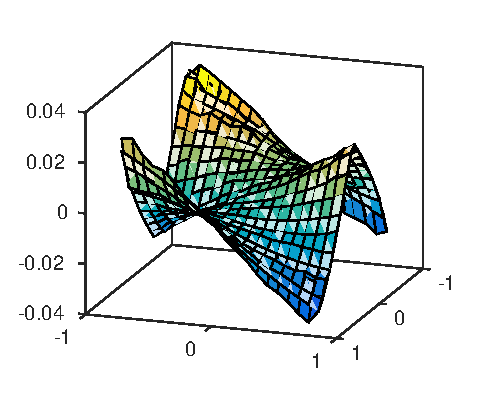
\includegraphics{plots/experiments/wing_rock/f_approx_surf.eps}
		%\caption{$\hat{W}_\varphi(t)$}
	\end{subfigure}
	\begin{subfigure}{0.5\textwidth}
		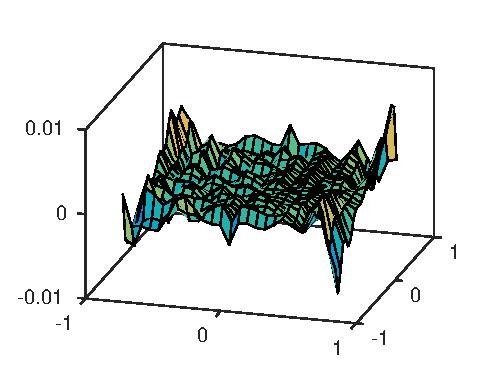
\includegraphics{plots/experiments/wing_rock/f_approx_error.eps}
		%\caption{$\hat{W}_\gamma(t)$)}
	\end{subfigure}
	\caption{Προσέγγιση της συνάρτησης $\varphi(x)$ (αριστερά) και το σφάλμα $\tilde{\varphi}(x)$ (δεξιά) στο πείραμα \textit{Wing Rock}.}
	\label{fig:wing_rock_phi_approximation}
\end{figure}

\subsubsection{Αποτελέσματα}
Μετά από προσομοίωση του συστήματος κλειστού βρόγχου για 50 περιόδους, στο Σχήμα \ref{fig:wing_rock_weights} παρουσιάζεται η χρονική εξέλιξη κάποιων βαρών $\hat{w}_{\varphi i}$ και της σταθεράς $\hat{w}_{\gamma 0}(t)$ συναρτήσει του χρόνου. Από το σχήμα είναι προφανές πως ο χρόνος εκπαίδευσης ήταν αρκετός για να συγκλίνουν τα βάρη του νευρωνικού δικτύου καθώς και η σταθερά  $\hat{w}_{\gamma 0}(t)$ που χρησιμοποιείται για την εκτίμηση της $\gamma(x)$.

Στο Σχήμα \ref{fig:wing_rock_phi_approximation} παρουσιάζεται η προσέγγιση της συνάρτησης $\hat{\varphi}(x)$ καθώς και το σφάλμα $\tilde{\varphi}(x)$. Όπως φαίνεται από τις δυο αυτές γραφικές παραστάσεις, το αποτέλεσμα της διαδικασίας αναγνώρισης της $\varphi(x)$ είναι πολύ ικανοποιητικό. Τέλος, παραθέτουμε έναν πίνακα (Πίνακας \ref{tab:stat_of_function_wing_rock}) με κάποια χαρακτηριστικά του σφάλματος προσέγγισης καθώς και της συνάρτησης $\varphi(x)$ εντός του συνόλου $\Omega_x$ ,έτσι ώστε να διευκολύνουμε την εξαγωγή συμπερασμάτων για την ποιότητα της προσέγγισης.

\begin{table}
	\centering
	\begin{tabular}{  c | c | c | c | c | c }
		& $\min_{x \in \Omega_x}$ & $\max_{x \in \Omega_x}$ & Εύρος Τιμών & $\max(\abs{\tilde{\varphi}(x)})$ & Σχετικό Σφάλμα \\ \hline
		$\varphi(x)$ & $-0.0325$ & $0.0332$ & $0.0657$ & $0.0084$ & $12.79\%$ \\
	\end{tabular}
	\caption{Στατιστικά στοιχειά προσεγγίσεων για το φαινόμενο  \textit{Wing Rock}}
	\label{tab:stat_of_function_wing_rock}
\end{table}

Όπως μπορούμε να δούμε και από τον Πίνακα \ref{tab:stat_of_function_wing_rock}, το μέγιστο ποσοστιαίο ή σχετικό  σφάλμα προσέγγισης εντός του $\Omega_x$ είναι $12.79\%$, γεγονός που επιβεβαιώνει πως τα αποτελέσματα είναι πολύ ικανοποιητικά.

Σχετικά με την ποιότητα προσέγγισης της $\gamma(x)$ η πραγματική τιμή της είναι ίση με $1/\theta_6 = 1.3333$ ενώ το βάθος $w_{\gamma 0}(t)$ συγκλίνει στην τιμή $1.3335$, που σημαίνει ότι και σε αυτή την περίπτωση το σχήμα αναγνωρίζει επιτυχώς την άγνωστη συνάρτηση.


\subsection{Ταλαντωτής \textit{Van der Pol}}
\label{exp:vdp}
Το δεύτερο πραγματικό σύστημα που θα μελετήσουμε είναι ένας οδηγούμενος ταλαντωτής \textit{Van der Pol}, το οποίο είναι ένα αρκετά κλασσικό σύστημα στην βιβλιογραφία του αυτομάτου ελέγχου. 

Το σύστημα αυτό είναι ένα μη-γραμμικό σύστημα δευτέρου βαθμού και περιγράφεται από τις εξισώσεις
\begin{equation}
\begin{split}
\dot{x}_1 &= x_2 \\
\dot{x}_2 &= \mu (1-x_1^2)x_2 - x_1 + 1+x_1^2+x_2^2)u(t)
\end{split}
\end{equation}
όπου $\mu$ θετική σταθερά. Στο πείραμα μας θεωρούμε πως $\mu = 1$. Όπως μπορούμε να δούμε η $g(x)$ σε αυτή την περίπτωση είναι συνάρτηση και των δυο καταστάσεων, συνεπώς το σύστημα δεν είναι τύπου \textit{Euler Lagrange}.


{\begin{wraptable}[16]{r}{0.3\textwidth}
		\centering
		\captionsetup{format=plain}
		\caption{Παράμετροι σχήματος αναγνώρισης για τον ταλαντωτή \textit{Van Der Pol}}
		\label{tab:vdp_schema_params}
		\begin{tabular}{ l | c }
			\hline\hline
			\text{Parameter} & Value \\ \hline\hline
			$k$             & $30$   \\ \hline
			$\lambda$       & $1 $   \\ \hline
			$\beta_{\varphi} \;\text{(bias)}$     & $10$ \\ \hline
			$\beta_{\varphi} \;\text{(gaussian)}$ & $50$ \\ \hline
			$\beta_{\gamma} \;\text{(bias)}$     & $5$ \\ \hline
			$\beta_{\gamma} \;\text{(gaussian)}$ & $20$ \\ \hline
			$\rho_0      $ & $4$  \\ \hline
			$\rho_\infty $ & $0.02$  \\ \hline
			$l           $ & $2$  \\ \hline
			$\textit{ΔΤ} $  & $1$ 	\\ \hline \hline	
		\end{tabular}
	\end{wraptable}

\subsubsection{Σχήμα Αναγνώρισης}
Για την αναγνώριση του παραπάνω συστήματος θα χρησιμοποιήσουμε δυο νευρωνικά δίκτυα RBF, ένα για την αναγνώριση της $\varphi(x)$ και ένα για την αναγνώρισης της  $\gamma(x)$. Καθώς και οι δυο άγνωστες συναρτήσεις εξαρτώνται από το πλήρες διάνυσμα καταστάσεων $x(t) =\bmqty{x_1(t),x_2(t)}^T$, θα χρησιμοποιηθεί το ίδιο διάνυσμα οπισοθδρομητών για τις προσεγγίσεις $\hat{\varphi}(x)$ και $\hat{\gamma}(x)$ όπως φαίνεται παρακάτω:
\begin{equation*}
\begin{matrix}
\hat{\varphi}(x,t)  = \hat{W}_{\varphi}^T(t) Z(x) & \text{και} & \hat{\gamma}(x,t) = \hat{W}_{\gamma}^T(t) Z(x) 
\end{matrix}
\end{equation*}
Σκοπός είναι η προσέγγιση του συστήματος στο σύνολο $\Omega_x = [-2,2] \times [-2,2] $. Για τον σκοπό αυτό, τα κέντρα $c_i$ των RBF συναρτήσεων του δικτύου $Z(x)$, επιλέγονται ως:
\begin{equation*}
	C =
	\bigtimes_{i = 1}^{2}
	 \begin{Bmatrix}
	-2 +  \frac{4}{9}k, \quad  k \in [0,1,...,9]
	\end{Bmatrix} 
%	\times
%	\begin{Bmatrix}
%	-2 +  \frac{4}{9}k, \quad  k \in [0,1,...,9]
%	\end{Bmatrix}
\end{equation*}
δηλαδή είναι το καρτεσιανό γινόμενο 10 ομοιόμορφα κατανεμημένων σημείων στο διάστημα $[-2,2]$, σχηματίζοντας έτσι ένα πλέγμα που καλύπτει ομοιόμορφα το $\Omega_x$. Οι υπόλοιποι παράμετροι του σχήματος προσομοίωσης φαίνονται στον Πίνακα \ref{tab:vdp_schema_params}.

\begin{figure}
	\begin{subfigure}{0.5\textwidth}
		% This file was created by matlab2tikz.
%
\definecolor{mycolor1}{rgb}{0.00000,0.44700,0.74100}%
\definecolor{mycolor2}{rgb}{0.85000,0.32500,0.09800}%
\definecolor{mycolor3}{rgb}{0.92900,0.69400,0.12500}%
\definecolor{mycolor4}{rgb}{0.49400,0.18400,0.55600}%
\definecolor{mycolor5}{rgb}{0.46600,0.67400,0.18800}%
%
\begin{tikzpicture}

\begin{axis}[%
width=0.761\textwidth,
height=0.65\textwidth,
at={(0\textwidth,0\textwidth)},
scale only axis,
xmin=0,
xmax=30000,
xlabel style={font=\color{white!15!black}},
xlabel={Time, $t$},
ymin=-0.6,
ymax=0.3,
axis background/.style={fill=white},
xmajorgrids,
ymajorgrids
]
\addplot [color=mycolor1, line width=1.2pt, forget plot]
  table[row sep=crcr]{%
0	0\\
2.1429703121903	0.0071388497017324\\
10.2144458867369	0.0071388497017324\\
12.6935285233594	0.0182630793096905\\
19.0024166006078	0.0182630793096905\\
21.6341449197353	0.0155200722547306\\
30.3065932697173	0.0157159249902179\\
33.2579855431177	-0.00130782568521681\\
108.841166682076	-0.00149401539601968\\
111.689288870384	0.0183589851731085\\
117.772474843459	0.0191556906938786\\
120.968578818061	0.0214065269392449\\
125.010576718396	0.049401769436372\\
130.125708129439	0.0512465794490709\\
134.021148090924	0.056102288144757\\
208.472820728439	0.055922178147739\\
211.539249661768	0.0712667731459078\\
219.836383353468	0.0712809293909231\\
224.131150829977	0.092217769659328\\
230.683618784802	0.0928618445432221\\
235.232270739052	0.098088785969594\\
310.101743421972	0.098005542615283\\
313.797145832774	0.106676715018693\\
319.831119357881	0.106676715018693\\
323.171506489693	0.113852398473682\\
329.701819856342	0.113380746995972\\
333.844214006116	0.115329776021099\\
408.020542798851	0.115323296115093\\
411.421409071962	0.120814957335824\\
417.864423662864	0.120395338588423\\
421.373701817352	0.122490657944581\\
431.877165995527	0.120724975087796\\
492.916461167741	0.120681762280583\\
510.868257740993	0.120795243030443\\
515.838572820398	0.124471925173566\\
521.107462027088	0.124564976144029\\
527.87067027939	0.123806445622904\\
531.763767883513	0.122593208227045\\
562.250432220222	0.122526486960851\\
609.683483558674	0.122546779046388\\
614.40414077344	0.125744855700759\\
627.512820855634	0.12555030612566\\
631.853310085095	0.124542370038398\\
678.084923536706	0.124487965353183\\
707.663192768276	0.124502559174289\\
711.877846211777	0.12760395058649\\
719.002974921601	0.127334732034797\\
723.524635392067	0.127750325169472\\
740.872404947742	0.127120364591974\\
806.437082491226	0.127129316460923\\
811.710224354163	0.129786016335856\\
818.729012973348	0.129538829609373\\
822.584666089948	0.130089292004413\\
829.447921885614	0.130126548381668\\
834.249671136608	0.129752841196023\\
908.32016420189	0.129763879263919\\
912.174388348241	0.131679016674752\\
919.376237631674	0.131679016674752\\
924.221934213645	0.132342884026002\\
941.230331266841	0.132143161859858\\
1006.07411180477	0.132159196789871\\
1011.37546106351	0.133840344868076\\
1018.86337179198	0.133618556130386\\
1022.94220741022	0.134339758675196\\
1040.54254986743	0.134163388647721\\
1107.0030412346	0.134169646338705\\
1111.89815581251	0.135528090570006\\
1119.026855753	0.135321325316909\\
1123.41616845127	0.135977576366713\\
1151.18483375865	0.135897598527663\\
1208.17608103233	0.135907849191426\\
1212.79840963939	0.136827820595499\\
1219.90195438917	0.136827820595499\\
1225	0.137403219392581\\
1255.94294843765	0.137357502710074\\
1307.86856223811	0.137364463513222\\
1312.5064435382	0.138053966547886\\
1319.28165371157	0.138053966547886\\
1323.10139945319	0.138459962319757\\
1391.11797563627	0.13847540585266\\
1410.92555771356	0.138232466411864\\
1421.84138523702	0.139584650616598\\
1438.38264153453	0.139540482432494\\
1506.57312321335	0.139547077385942\\
1511.70017968949	0.14012077256848\\
1518.91323295227	0.139967453113059\\
1523.12325550624	0.140533437988779\\
1620.72318385332	0.140942975805956\\
1631.75471775699	0.141547105919017\\
1710.79978572428	0.14154698278071\\
1743.7443238451	0.142194481930346\\
1818.51036044772	0.142293145756412\\
1822.91449497836	0.142599933504243\\
1901.47028032636	0.142776519711333\\
1919.94303399767	0.142804373037507\\
1931.2273978423	0.143364202998782\\
2017.76379775714	0.143319069633435\\
2022.21919173714	0.143547698273323\\
2127.96818706816	0.143763543015666\\
2132.27725086937	0.143998189407284\\
2230.71941612057	0.144203299973015\\
2247.20160580119	0.144363807885384\\
2316.72818066891	0.144175914443622\\
2321.61841416669	0.14471129960657\\
2332.91047548936	0.144769646452914\\
2520.26243371515	0.144842296969728\\
2538.50572915302	0.145314137778769\\
2717.21980816186	0.14531021444418\\
2721.87048550599	0.145863568184723\\
2729.27147467898	0.14564317964323\\
2733.92323082226	0.145897690443235\\
2917.0023110632	0.145821260601224\\
2921.67787110436	0.146328202517907\\
2933	0.146315937152394\\
3229.26479536984	0.146490394741704\\
3240.59900200955	0.146706111769163\\
3309.92693583981	0.14670821818072\\
3314.50315311764	0.146330488649255\\
3327.00391117065	0.146647319848853\\
3338.51577087246	0.146820270176249\\
3409.00607541228	0.146822753707966\\
3412.60160627479	0.146426923001854\\
3423.52180546665	0.146701838257286\\
3469.23213376801	0.146894222947594\\
3506.09107654371	0.146897384267504\\
3510.95060424976	0.146335687037208\\
3516.7830118806	0.146465378711582\\
3521.32582004987	0.147106971213361\\
3532.51270457872	0.14706204689719\\
3608.80539905221	0.147068642396334\\
3612.32217278336	0.146651755330822\\
3622.96847715085	0.14695218169436\\
3684.3313860985	0.147092240615166\\
3710.373441808	0.14709852647502\\
3716	0.146682467027858\\
3721.12245391358	0.147217261870537\\
3732.74690362606	0.14722555492699\\
3808.47611844205	0.147233418618271\\
3812.27498387385	0.146802149432915\\
4029.8779589236	0.147108113382274\\
4053.27416341057	0.147216813555133\\
4109.49806211522	0.147229400437936\\
4113.36759002267	0.146811788799823\\
4120.15878863379	0.146811788799823\\
4131.1192481148	0.147417174463044\\
4271.26430865099	0.147438995125412\\
4309.00323328197	0.147444199865276\\
4312.827772976	0.146988993834384\\
4319.77101667516	0.146988993834384\\
4324.93485008113	0.147498401242046\\
4380.16291541682	0.147709288488841\\
4406.92531620958	0.147710349352565\\
4411.35875606601	0.147328756378556\\
4417.73247370151	0.147293901889498\\
4421.96696244987	0.14770542932456\\
4428.86051845579	0.147378196390491\\
4439.77156477698	0.14756986213979\\
4509.0383319938	0.147581904522667\\
4512.86138130377	0.147141880624986\\
4709.7177956034	0.14714850699238\\
4714.1036375142	0.146737851377111\\
4726.73586135255	0.146983204645949\\
4738.3876561124	0.147134091446787\\
4808.19896336354	0.147140337499877\\
4812.2553915837	0.14670732045488\\
4819.1859545513	0.14670732045488\\
4824	0.14713791658869\\
4883.92308228054	0.147343067197653\\
4910.55972756127	0.1473494181555\\
4916.00330713585	0.146936012042715\\
4921.24138306996	0.147345055698679\\
4931.95844957148	0.147258216595219\\
5007.00093248662	0.147258842040173\\
5011.62899045114	0.146823954724823\\
5018.37065311713	0.146802177347126\\
5022.78953169446	0.14734312571818\\
5108.74627681381	0.147426047038607\\
5113.0343599325	0.146990504861606\\
5119.61561598695	0.146990504861606\\
5124.91453528286	0.147434849783167\\
5209.90839354102	0.147571390061785\\
5216.24543602869	0.1471375166293\\
5221.25546140975	0.147516813154652\\
5232.1260927229	0.147406572501495\\
5308.38793498067	0.147412837974116\\
5312.45721138182	0.146951200382318\\
5319.39422424302	0.146951200382318\\
5323.80358989279	0.147400147965527\\
5382.42780921902	0.147533836170624\\
5409.57733857635	0.147539120163856\\
5415.01853605729	0.14707172267299\\
5421.01659445115	0.147729915450327\\
5427.86478395671	0.147221657811315\\
5442.07664864263	0.147336476748023\\
5507.64115087972	0.147348703125317\\
5512.00259568214	0.146894633944612\\
5616.40172690298	0.146772413067083\\
5621.30468205311	0.147523131290654\\
5632.08739758415	0.14736386775985\\
5707.95140895514	0.147373398944183\\
5712.34631878633	0.146951714767056\\
5730.57022306823	0.147170909396664\\
5744.24033274177	0.147342294963892\\
5810.0902202252	0.147350688886945\\
5816.15466093113	0.146913486834819\\
5821.20237459952	0.147275307437667\\
5831.84173305134	0.147122430455056\\
5929.19897097909	0.147227087949432\\
5939.24298404938	0.147372025174263\\
6007.30525959839	0.147376554530638\\
6012.1447243853	0.146947383327642\\
6030.21780977659	0.147258577493631\\
6043.29076973042	0.147392501887225\\
6109.81703562	0.147399953697459\\
6116.00344287793	0.146967418233544\\
6121.31178211188	0.147482147600385\\
6131.85203342423	0.147264165672823\\
6416	0.146812049897562\\
6421.03520784756	0.147434228401835\\
6431.22904113229	0.147437202955189\\
6751.78603862941	0.147428991582274\\
6809.10110935699	0.147437058236392\\
6813.93890827283	0.1470638836945\\
6831.05502440718	0.14737726410749\\
6868.6467224502	0.147426966814237\\
6906.60931277213	0.14743624386756\\
6911.94791900303	0.147059903094487\\
7017.82212516034	0.146841234545718\\
7021.96836690782	0.14760730218768\\
7032.35024055289	0.147305912334559\\
7108.51371387645	0.147315309837722\\
7112.83159545859	0.146918090598774\\
7119.94133429677	0.146918090598774\\
7131	0.147351934843755\\
7191.0163446273	0.147386914526578\\
7206.82191335597	0.147393657844077\\
7211.84057310519	0.146982307342114\\
7229.63389416331	0.147244696228881\\
7243.22881067909	0.1473439294532\\
7310.89411168927	0.147450353182649\\
7317.74168893769	0.146902997374127\\
7322.02083579929	0.147366015291482\\
7333	0.147226439599763\\
7405.56431418971	0.147232755825826\\
7411.45992800876	0.146880429034354\\
7429.74514620524	0.147156116185215\\
7449.14046552766	0.147247921344388\\
7611.14388079901	0.146918095710134\\
7633.41826141419	0.147201340241736\\
7704.57106112706	0.147208312329894\\
7711.36595432442	0.14681215951714\\
7718.31165196934	0.146800430677104\\
7722.48067772292	0.147210785460629\\
7829.42503329036	0.14746412565728\\
7852.66170164884	0.147527797340445\\
7905.23476009957	0.147535712276294\\
7911.15567496596	0.147166168902913\\
7918.20892673814	0.147145507577079\\
7922.14401669169	0.147658901965769\\
7990.48006294942	0.147733367026376\\
8005.00357152856	0.147741411714378\\
8011.37958121969	0.147348527887516\\
8044.16254031615	0.147583364869206\\
8106.15599899262	0.147591659711907\\
8111.82982684387	0.147190078896529\\
8119.00540560564	0.147170407384692\\
8123.57372794385	0.147745479764126\\
8269.83822618062	0.147641776871751\\
8308.16728886086	0.147647918107396\\
8312.91868559702	0.147234720701817\\
8420.58818214518	0.147206669069419\\
8431.17292306665	0.147678340312268\\
8729.32139585512	0.147806548753579\\
8807.44856303841	0.147839544231829\\
8811.89405545056	0.14752405998297\\
8869.68049735541	0.147822940776678\\
9009.09745142378	0.147826311454992\\
9013.85416619627	0.14744749345482\\
9026.33362305641	0.147760498792195\\
9056.08988484127	0.147821377398941\\
9114.23414617582	0.147506908633659\\
9121.01195749822	0.148467047358281\\
9131.92915517115	0.147992958631221\\
9420.16745903611	0.147769305513066\\
9431.29525080641	0.14822779370661\\
9516.0050167573	0.147885818387294\\
9521.13500243677	0.148625806923519\\
9532.01367893672	0.148319464267843\\
9806.13883715562	0.148296957544517\\
9811.74699103655	0.147964093557675\\
9830.51452389086	0.148229272563185\\
9854	0.148312566107052\\
10120.7545853081	0.148270363024494\\
10131.6222818175	0.148702281992882\\
10316.1556153589	0.148274218066945\\
10321.3919837539	0.149013916994591\\
10332.211355176	0.148697991819063\\
10417.7469963724	0.148360471506749\\
10421.8979925171	0.149131697442499\\
10433	0.148769980398356\\
10610.6625766366	0.148681371938437\\
10617.1220772062	0.148349372833763\\
10621.813189233	0.149027957970247\\
10632.810863959	0.148673275303736\\
10710.6673669835	0.14868353741258\\
10717.6455512177	0.148318767856836\\
10721.8473445434	0.149068073780654\\
10732.9352452412	0.148713011327345\\
10811.0009247094	0.14845289718869\\
10817.8071365345	0.148361758772808\\
10821.9101985973	0.149187752987928\\
10833.3414876574	0.148838431181503\\
11217.6944235344	0.148827783974411\\
11222.0006662482	0.149594482561952\\
11233.1858615523	0.149188501836761\\
11317	0.148878619434981\\
11321.7820358563	0.149607695013401\\
11333.1381017241	0.149228972204583\\
11608.8877882458	0.14919037594882\\
11613.7156802243	0.148882624202088\\
11720.022167838	0.148846892385336\\
11731.1807133905	0.149322322351509\\
11914.0275645939	0.149092180916341\\
11920.895694693	0.148915513753309\\
11927.5819006494	0.149432137804979\\
11951.7891076006	0.149374211610848\\
12015.4737326088	0.149086760698992\\
12021.2317557584	0.149890527842217\\
12032.0121434712	0.149508341455658\\
12117.1485798951	0.14924225921277\\
12121.8236670084	0.14986891080116\\
12132.8852592507	0.149542838196794\\
13210.698692775	0.149437535761535\\
13217	0.149198301787692\\
13221.5901071449	0.149988932422275\\
13232.9061687686	0.149590865450591\\
13410.7296126246	0.149414602074103\\
13417.012313751	0.149134409683029\\
13421.6388809554	0.149673753225215\\
13432.9347136308	0.149325842980033\\
13517.7292969227	0.149062210723059\\
13522	0.149836674321705\\
13533.9389911019	0.149442208414257\\
13711.2552150563	0.1491113058255\\
13718.0029903344	0.14908969755561\\
13722.0503271158	0.149626863912999\\
13818.2368269386	0.149275643019791\\
13822.8124934388	0.14957746998698\\
13859.2722739062	0.149511419371265\\
14117.4025860862	0.149322518114786\\
14122.007407639	0.150065194124181\\
14133.8430911628	0.149700133631995\\
15016.0915212915	0.149675517215655\\
15021.2371223803	0.150245756900404\\
15032.3066374784	0.149826767188642\\
15708.4524200534	0.149693480798305\\
15719.9470970476	0.149480350901285\\
15731.2589920798	0.149612841345515\\
15916.0735731303	0.149484237550496\\
15921.2040183493	0.150001195255754\\
15932.1810432599	0.149507268306479\\
16317	0.149517698850104\\
16321.5897547781	0.15022728970871\\
16332.7687891868	0.149786648704321\\
16416.055977529	0.149583284637629\\
16421.2790418804	0.150265498381486\\
16432.3370418448	0.149736215989833\\
16707.9572428495	0.149572123627877\\
16719.2520929173	0.149386551001953\\
16723.9785046391	0.149764934678387\\
16759.708042575	0.149705861254915\\
17116	0.149393447536568\\
17121.2799671293	0.150103907140874\\
17132.279280251	0.149621500571811\\
17916.3250388274	0.149468014260492\\
17921.4532267201	0.150022133559105\\
17932.8001713184	0.149588302254415\\
18117.3576197058	0.14929422003479\\
18121.8558473103	0.1500514244035\\
18133.5441582504	0.149578665306763\\
18505.6407456067	0.149427431311778\\
18518.1015782541	0.149205315083236\\
18522.5197379783	0.149455569197016\\
18715.8335373007	0.149194949161028\\
18721.1861742546	0.149817326586344\\
18731.9581554258	0.149321701192093\\
19117.1436643781	0.149448484164168\\
19121.7852832871	0.150218021812179\\
19132.925137194	0.149700696514628\\
19320.012880577	0.149671075781953\\
19326.3872052117	0.150056386897631\\
19342.0496159587	0.149945729390311\\
19414.3672070673	0.149758148632827\\
19421	0.150290239293099\\
19431.7558508557	0.149696649477846\\
19516	0.149543301926315\\
19521.1718718575	0.150331338241813\\
19532.0067509614	0.149872617126675\\
19617.6882551574	0.149706693373446\\
19621.9003575912	0.15027776520219\\
19632.9833802659	0.149751779779763\\
20215.9730688005	0.149606067538116\\
20221.1732766805	0.150235999142751\\
20232.1998366623	0.149766877926595\\
20317.0123180531	0.149657964200742\\
20321.6507854216	0.150358280738146\\
20332.0533661824	0.149851881258655\\
20417.3234978122	0.149690349822777\\
20421.7959707443	0.150210588024493\\
20432.8986962638	0.14973887510132\\
20517.0482848641	0.149556904147175\\
20521.6597619186	0.150174141803291\\
20532.8802415508	0.149697688411834\\
21215.3011755993	0.149508196333045\\
21221.1802701434	0.150099540715019\\
21231.9422239065	0.149585706039943\\
21317.2115481803	0.14945858869396\\
21321.6417395426	0.150320275024569\\
21332.3263933206	0.14981181264011\\
21417.351910062	0.149673880758201\\
21421.8266423857	0.150352028187626\\
21432.898581737	0.149807867321215\\
21908.2284091572	0.149530665377824\\
21919.3520714009	0.149394914515142\\
21930.003641338	0.149418455239356\\
22309.7613955523	0.14970066540991\\
22314.9858168694	0.149562443424657\\
22321.0662034484	0.149839804340445\\
22342.8092057293	0.149528568214009\\
22517.1242634101	0.149279045934236\\
22521.7323807462	0.149975053944218\\
22532.7924571718	0.149507797184924\\
23019.1942148502	0.14940173422292\\
23023.9799485888	0.14987298712731\\
23051	0.149780505958915\\
23818.9468793398	0.149684970096132\\
23822.9863168336	0.150145744566544\\
23850.4841732055	0.150078534559725\\
24017.1160364527	0.149973589843285\\
24021.6942214265	0.150516027049889\\
24032.6955024185	0.150007922871737\\
24117.3530203838	0.149813406773319\\
24121.6466749615	0.150487465361948\\
24132.4013769486	0.149943094416813\\
24518	0.149689470319572\\
24522.0020996167	0.150469641364907\\
24533.0037678317	0.149946948098659\\
24718.0313625256	0.149750540953391\\
24722.0016286153	0.150588291042368\\
24733.0989235541	0.149974357926112\\
25109.9520998524	0.149656424637215\\
25115.6937658416	0.149502311192919\\
25121.0913230378	0.15016449252289\\
25143	0.14980605956589\\
25216.0333427894	0.149660259761731\\
25221.2110718401	0.150385856919456\\
25231.9797937119	0.14981295065445\\
25315.4391974248	0.149677203702595\\
25320.9025739178	0.149460640972393\\
25327.2463062733	0.150053373199626\\
25342.4469990413	0.149958592133771\\
25416	0.149792894844722\\
25421.1352214631	0.150572188424121\\
25432.2136457829	0.150126758111583\\
25515.3617295063	0.149987653581775\\
25521.1485498463	0.150498379334749\\
25531.63635359	0.150065205423743\\
25616.2452317043	0.149931996005762\\
25621.2564436163	0.150557157208823\\
25632.1647663355	0.150015386414452\\
26316.8687098101	0.149919577928813\\
26321.4305710401	0.150491032945865\\
26332.3184438609	0.149934226821642\\
27810.2757237357	0.149694014802662\\
27820.8877865944	0.149398262339673\\
27831.8180622961	0.14965244263658\\
28006	0.14954063996629\\
28017.9398934959	0.149379275004321\\
28022.0466987695	0.14957593190411\\
28067.8463567904	0.149406633790932\\
28414.9687831391	0.14921984682951\\
28421.0003162165	0.149855618092261\\
28431.8648451467	0.149394727101026\\
28517.4779562238	0.149262612281746\\
28521.6316079654	0.150008226410137\\
28532.6654438838	0.149396612432611\\
28917.8760863861	0.149105523487378\\
28921.7419887424	0.149923798762757\\
28932.6796630234	0.149318770083482\\
29210.4238771097	0.149010032677324\\
29217	0.148906944246846\\
29221.4878685808	0.149489678045938\\
29232.0066601752	0.148933217100421\\
29816.5308583665	0.148965406704519\\
29821.3596718873	0.149414440587861\\
29832.2137285266	0.14876896286296\\
29998.5116797138	0.148684788811806\\
};
\addplot [color=mycolor2, line width=1.2pt, forget plot]
  table[row sep=crcr]{%
0	0\\
2.1429703121903	0.0959209359534725\\
30.3065932697173	0.0961071037381771\\
33.2579855431177	0.0326556620893825\\
38.856075102387	0.0212785567346145\\
41.1680613500212	0.0047146553042694\\
46.0485718023447	-0.142023967368004\\
52.3843725863771	-0.177788716668147\\
58.0545783998896	-0.246763924606057\\
60.9123342033199	-0.22959320229711\\
117.772474843459	-0.22959320229711\\
120.968578818061	-0.226612948623369\\
130.125708129439	-0.226612928883696\\
134.021148090924	-0.208819801151549\\
140.046488349912	-0.205965136072336\\
144.474555678571	-0.183359787763038\\
150.889071163801	-0.1880390415281\\
156.402175379095	-0.199119066404819\\
161.015668957811	-0.199948387115001\\
219.836383353468	-0.199948387115001\\
224.131150829977	-0.198462997264869\\
230.683618784802	-0.196986009465036\\
235.232270739052	-0.187971109851787\\
240.801411190478	-0.188129158203083\\
246.124790787722	-0.153071140372049\\
251.25142180188	-0.153091240332287\\
257.567764332773	-0.150042559100257\\
261.634361819251	-0.152691012161085\\
319.831119357881	-0.152691012161085\\
323.171506489693	-0.152014212602808\\
329.701819856342	-0.152014212602808\\
333.844214006116	-0.149548296267312\\
340	-0.149778679184237\\
343.99687958898	-0.13815499420889\\
349.994714028755	-0.136834556255053\\
354.107547577307	-0.13423627197335\\
359.712273808556	-0.136005043827026\\
417.864423662864	-0.135995300210197\\
421.373701817352	-0.135491307777556\\
428.077185216498	-0.135491307777556\\
431.877165995527	-0.131650952764176\\
438.729790616377	-0.135560729795543\\
442.278039469038	-0.130693872735719\\
447.766527706597	-0.128451318283624\\
451.090069126785	-0.131080640341679\\
454.746568083894	-0.131253242409002\\
459.793861401424	-0.132386264922388\\
515.838572820398	-0.132386401703116\\
521.107462027088	-0.131928733560926\\
527.87067027939	-0.131928733560926\\
531.763767883513	-0.128160298136208\\
537.742638090127	-0.131627246453718\\
541.344829898393	-0.128906194717274\\
545.355712957917	-0.127380947062193\\
549.864808520368	-0.129801601036888\\
553.661844136259	-0.130914600518736\\
558.915672403396	-0.131650143179286\\
568.769765201821	-0.131489558076282\\
620.745964045225	-0.131190939318913\\
627.512820855634	-0.131116267351899\\
631.853310085095	-0.127899700812122\\
638.43375335271	-0.130660153205099\\
642.190589693146	-0.126715544880426\\
647.81676004254	-0.126934283729497\\
651.723239909541	-0.126667990807618\\
657.50593916958	-0.129582945883158\\
681.353659528068	-0.129521711231064\\
730.368192559952	-0.129251550468325\\
740.872404947742	-0.127129813499778\\
745.219982828661	-0.124498015622521\\
750.577034095531	-0.126092011345463\\
755.857574539285	-0.126494141168223\\
777.00290432771	-0.126403293463227\\
829.447921885614	-0.126217210203322\\
834.249671136608	-0.124952142370603\\
840.373504782932	-0.12505883167978\\
844.419693614942	-0.121747133547615\\
850.11647017195	-0.123163390857371\\
890.755841466762	-0.122978063831397\\
930.649139281082	-0.122742062998441\\
941.230331266841	-0.120473188260803\\
947.693673079786	-0.119132433334016\\
951.83587583917	-0.118652469496737\\
958.046247733331	-0.120043556038581\\
972.315610546346	-0.11994854371369\\
1029.90835891964	-0.119864008025615\\
1034.98903117405	-0.118672196160333\\
1040.54254986743	-0.118714141455712\\
1046	-0.116236016780022\\
1050.98992346409	-0.117751999958273\\
1061.24069831668	-0.117301584868983\\
1130.31443625383	-0.117255793036747\\
1135.65246562484	-0.116060714521154\\
1140.93931589019	-0.115450199406041\\
1146.62482579601	-0.114416214128141\\
1151.18483375865	-0.115364897636027\\
1179.01126471064	-0.115390663133439\\
1225	-0.11538004076283\\
1230.76274806616	-0.114449627173599\\
1240.66882618296	-0.114133258852235\\
1245.87698656711	-0.11285612390202\\
1250.55622544931	-0.114277568092803\\
1261.04291372417	-0.114024587546737\\
1329.86104208577	-0.114021805817174\\
1333.86155719839	-0.112949520931579\\
1339.59939138869	-0.112724676011567\\
1343.48228525082	-0.111344815279153\\
1349.54322408807	-0.112777936625207\\
1359.60071979818	-0.112945073913579\\
1363.7272661763	-0.112613914574467\\
1428.82206480029	-0.112618734186981\\
1432.19104398142	-0.111530997266527\\
1438.38264153453	-0.111290907887451\\
1441.97099862661	-0.110486263649364\\
1448.20541566692	-0.110856644958403\\
1452.06755204638	-0.110360964197753\\
1458.6929682482	-0.111697961594473\\
1462.07847445008	-0.111394178340561\\
1530	-0.111419453936833\\
1534.0987541984	-0.110181297004601\\
1539.65032105379	-0.110040164228849\\
1543.6070206236	-0.108813618604472\\
1549.51633679582	-0.110450101372408\\
1553.30815745178	-0.110735961454338\\
1572.49889027333	-0.110480458100938\\
1627.1243450965	-0.110511082049925\\
1631.75471775699	-0.109574015037651\\
1638.08584955521	-0.10923239944168\\
1642.00687855725	-0.108336064757168\\
1648.26922146963	-0.109315065354167\\
1652.21906805947	-0.109326946589135\\
1658.6621467859	-0.110078071753378\\
1662.66893467667	-0.109670955083857\\
1728.79962268898	-0.109708710104314\\
1733.12922262778	-0.108582550190476\\
1739.56512403056	-0.108154370209377\\
1743.7443238451	-0.107018091443024\\
1749.7311371381	-0.108999595606292\\
1759.91465074835	-0.108831011595612\\
1829.92032747495	-0.108870325024327\\
1834.82217032371	-0.107562023884384\\
1846.22153867136	-0.107002619122795\\
1851	-0.108129520460352\\
1860.74322548409	-0.107940320267517\\
1926.03348978527	-0.107968617725419\\
1931.2273978423	-0.10702704248979\\
1937.78120462559	-0.106592208961956\\
1941.96149228081	-0.105852157183108\\
1948.12226568695	-0.106753017553274\\
1951.97553377745	-0.106069526129431\\
1958.11043262636	-0.107054389478435\\
1972.52087569288	-0.106970838754933\\
2029.32100501169	-0.107002334767458\\
2033.90819169728	-0.105958519216074\\
2046.0034418327	-0.105439346192725\\
2050.76334812981	-0.106863134547893\\
2056.00342556328	-0.106552049062884\\
2071.47548154816	-0.106667380354338\\
2127.96818706816	-0.106710476513399\\
2132.27725086937	-0.105831049666449\\
2139.01312156839	-0.105324597367144\\
2142.7315033376	-0.104149734015664\\
2149.04603674252	-0.105961256533192\\
2152.78893863173	-0.105795500348904\\
2158.86604718418	-0.106407349841902\\
2169.71362382936	-0.106198612091248\\
2230.71941612057	-0.106126952890918\\
2236.90995947508	-0.10490721442693\\
2241.38029792706	-0.104412092052371\\
2271.43428933035	-0.105581823354441\\
2328.83566180742	-0.105635477026226\\
2332.91047548936	-0.104686565806333\\
2339.50504133006	-0.104191418253322\\
2343.80653338398	-0.103460589853057\\
2349.46446689618	-0.105400446354906\\
2359.25692482376	-0.105713983532041\\
2363.35022257851	-0.10537373578336\\
2424.17948257758	-0.105410941210721\\
2431	-0.104575454657606\\
2437.34417895164	-0.104179545563966\\
2441.67777844047	-0.103542300734262\\
2467.06276130875	-0.10510975671059\\
2527.21198669675	-0.105164245549531\\
2531.95625267276	-0.104178351335577\\
2538.50572915302	-0.103619510813587\\
2542.33328867969	-0.102426751629537\\
2548.24850962279	-0.103860816398083\\
2552.16902505396	-0.103954847949353\\
2558.10381614968	-0.104557598071551\\
2572.24985082022	-0.104468482386437\\
2628.59969442289	-0.104513405887701\\
2633.0178668212	-0.103539035128051\\
2639.74385113236	-0.103042354639911\\
2643.3356539065	-0.102388243791211\\
2649.00728168863	-0.104088461765059\\
2652.42114148101	-0.10393974039107\\
2662.33827069417	-0.104314986878308\\
2729.27147467898	-0.104374225484207\\
2733.92323082226	-0.103396227663325\\
2743.92005217004	-0.102575105880533\\
2749.31943362875	-0.103849326267664\\
2759.01311924212	-0.104122256107075\\
2763.25693350876	-0.103844871118781\\
2829.79182787078	-0.10388256002625\\
2835.16444759464	-0.102552506268694\\
2844.016173026	-0.102392442426208\\
2849.40549482055	-0.103601176168013\\
2853.00634138237	-0.103291722640279\\
2858.73984368716	-0.103829491690703\\
2862.88422507771	-0.103583959386015\\
2928.60375440571	-0.103637438132864\\
2933	-0.102692602795287\\
2939.81552733111	-0.102165364176471\\
2943.6996673279	-0.101498599091428\\
2949.14859679667	-0.103106351845781\\
2952.35600684679	-0.10289176954393\\
2962.2831337896	-0.103109764208057\\
3029.07312743537	-0.103160459784704\\
3033.62986527287	-0.102090184383997\\
3039.79884956768	-0.101696948855533\\
3043.66597899804	-0.100811209686071\\
3049.23767253396	-0.102538980219833\\
3052.8264182937	-0.102333447313868\\
3062.36461098883	-0.102491765832383\\
3128.09856334825	-0.10254180080301\\
3132.08592397109	-0.101565107586794\\
3138.83180587057	-0.101121677838819\\
3142.26929304341	-0.100112743089994\\
3148.00422267788	-0.102002296309365\\
3151.4096149136	-0.101306634660432\\
3161.09762071128	-0.102146977071243\\
3229.26479536984	-0.102209420118015\\
3234	-0.101066929299122\\
3240.59900200955	-0.100750068388152\\
3244.53344166362	-0.101006296805281\\
3249.7250084254	-0.10213042754549\\
3253.13145457137	-0.101733531770151\\
3258.7959171048	-0.102187614495051\\
3262.82084595679	-0.101889915833453\\
3327.00391117065	-0.101953111152397\\
3331.79647791024	-0.100941002881882\\
3338.51577087246	-0.100511437201931\\
3342.26093165005	-0.0994286553213897\\
3347.82420693314	-0.101489695338387\\
3351.38613238964	-0.100856345539796\\
3361.00101084223	-0.101542469732522\\
3430.06874570972	-0.101608365683205\\
3436.00344218671	-0.100280118713272\\
3441.00695998884	-0.0998209878343914\\
3446	-0.10025814747496\\
3450.01434888058	-0.101577736095351\\
3469.23213376801	-0.101223208199372\\
3528.32770629848	-0.101286709341366\\
3532.51270457872	-0.10046846250043\\
3539.22165062591	-0.0999426892776683\\
3542.74872436703	-0.0988412531078211\\
3548.32105712704	-0.10066502992413\\
3551.97099319949	-0.10018433877849\\
3561.27952742534	-0.10107390873236\\
3629.82837361279	-0.101147948258586\\
3635	-0.0998320700600743\\
3644.5088083644	-0.0998439150243939\\
3649.66265671154	-0.100837446916557\\
3652.89449475812	-0.100364463527512\\
3668.00331368189	-0.100657186660101\\
3728.16968269358	-0.100722075087106\\
3732.74690362606	-0.0998612474395486\\
3743.02257541929	-0.098590257075557\\
3748.7544227753	-0.100457127256959\\
3752.03286567183	-0.0995419322680391\\
3761.27670604578	-0.100316736934474\\
3829.96083016896	-0.100383454329858\\
3836	-0.0991253389256599\\
3841.12971036832	-0.0987595423393941\\
3846.26648357925	-0.099217961087561\\
3850.33223347291	-0.100441032758681\\
3863.25520111353	-0.100171416688681\\
3928.28130103319	-0.100236297064839\\
3932.68411641294	-0.0993536622372631\\
3939.29043884383	-0.0989773594956205\\
3942.88294529316	-0.0983525465780986\\
3948.86415551575	-0.100037149160926\\
3952.12346220194	-0.0991081172796839\\
3957.15676172539	-0.0998028745707416\\
3966.62653886499	-0.100001935014006\\
4029.8779589236	-0.100078088809823\\
4035.80573389588	-0.0987985511710576\\
4040.76785759918	-0.0983524775037949\\
4044.64782244763	-0.0988839892816031\\
4049.82343968829	-0.100019317815168\\
4078.95464740375	-0.0995878455942147\\
4126.07403544831	-0.0996598763013026\\
4131.1192481148	-0.0987965836793592\\
4141.78612336691	-0.0978686319722328\\
4147.56361329904	-0.0987206264871929\\
4151.33871470614	-0.0985360444792605\\
4154.83607408533	-0.0991283416515216\\
4163.90520474617	-0.0993371507574921\\
4229.01689651387	-0.0994123275486345\\
4233.35662614447	-0.0983558065745456\\
4239.96295366641	-0.0979921681282576\\
4243.35417778067	-0.0970925830370106\\
4249.21803284427	-0.0989520414805156\\
4252.69929817252	-0.0987377020683198\\
4271.26430865099	-0.0988303620288207\\
4324.93485008113	-0.0988878637508606\\
4330.85649400827	-0.0979375996103045\\
4341.21037788334	-0.0970949151851528\\
4350.50664633387	-0.0989515991641383\\
4391.24785145948	-0.0986200611660024\\
4428.86051845579	-0.0986767523099843\\
4432.97876076237	-0.0976763177095563\\
4443.07087693282	-0.096718777447677\\
4449.0298897647	-0.0983046165929409\\
4452.34729749643	-0.0980006342906563\\
4467.14174784977	-0.0982714614183351\\
4530.72785846018	-0.0979464009506046\\
4541.28185642152	-0.0966415647199028\\
4546.63393687929	-0.0973503699424327\\
4551.12499528719	-0.0985067266447004\\
4554.1199873136	-0.0981732508880668\\
4559.22550630149	-0.0983363721752539\\
4563.21280838384	-0.0980755364325887\\
4629.90562375734	-0.0981401729877689\\
4635.21514278452	-0.0968263070571993\\
4640.634208407	-0.0966448892650078\\
4644.47180684014	-0.0969150712917326\\
4649.72343677032	-0.0979776310814486\\
4652.86506552183	-0.0974702030543995\\
4667.68332508349	-0.0975551475457905\\
4726.73586135255	-0.0976320017653052\\
4731.51260374806	-0.0966901049287117\\
4738.3876561124	-0.0963464378546632\\
4742.09721022311	-0.0956891608584556\\
4747.8522150176	-0.0972098130660015\\
4751.41846702668	-0.0966006895141618\\
4760.1838975986	-0.0973921793047339\\
4830.48381420751	-0.0974581514237798\\
4836.03350604084	-0.0961170145747019\\
4840.91748290742	-0.0956813822776894\\
4845.26536010232	-0.0962390146887628\\
4850.64649822661	-0.0973559770573047\\
4862.71745356912	-0.0968614067860472\\
4927.92909596712	-0.0969287813568371\\
4931.95844957148	-0.0959968508577731\\
4938.81801268894	-0.095820895738143\\
4942.04054126195	-0.095120493122522\\
4948.18710877003	-0.0964778996676614\\
4951.77425677891	-0.0960498601016297\\
4960.28989055551	-0.0967304210171278\\
5029.61561215179	-0.0968034072066075\\
5033.88725178999	-0.0957660076419415\\
5040.02683326294	-0.0953987408756802\\
5043.35398406207	-0.0947294241632335\\
5049.15801722012	-0.0966034496814245\\
5057.55489448957	-0.096301754743763\\
5070.90711728311	-0.0963943042879691\\
5130.56336047161	-0.0964746431563981\\
5136.31707765498	-0.0951915363548324\\
5141.0756308044	-0.0948201917854021\\
5145.11442350142	-0.0953983203980897\\
5150.53384580279	-0.0966106119194592\\
5172.1854186452	-0.0961748211993836\\
5228.00988112635	-0.0962337564124027\\
5232.1260927229	-0.0952574591974553\\
5238.80800988311	-0.0948805084735795\\
5242.23545242564	-0.0937645369340316\\
5248.15888714893	-0.0958505924645578\\
5251.68885389107	-0.0952783366556105\\
5259.98668477049	-0.0959960651380243\\
5329.94670894251	-0.096062431424798\\
5334.45168538485	-0.094820551428711\\
5340.42889531568	-0.0945975505637762\\
5343.78146229533	-0.0939822031432413\\
5349.21322739687	-0.0957916920815478\\
5352.4149777751	-0.0955472607201955\\
5378.25614234969	-0.0956272765142785\\
5427.86478395671	-0.0957077629936975\\
5432	-0.0947340936036198\\
5438.63669331452	-0.0943778058390308\\
5442.07664864263	-0.0936481098688091\\
5447.84897313344	-0.0952970578582608\\
5451.58595579535	-0.0947436243004631\\
5455.69732534187	-0.0953172277077101\\
5469.78283363634	-0.0954322829420562\\
5530.32593737709	-0.0955033461214043\\
5535.353587993	-0.0942348973949265\\
5540.67438988352	-0.0940502832818311\\
5544.43703722425	-0.0944823589888983\\
5549.79476783698	-0.0958440817485098\\
5562.31161613313	-0.0953857180647901\\
5628.14688225833	-0.095453614667349\\
5632.08739758415	-0.0944649477969506\\
5638.50686246919	-0.0940883160510566\\
5641.85999704869	-0.0935021707155101\\
5647.44793161612	-0.0941690215731796\\
5651.0898875838	-0.0954776210601267\\
5654.38573660336	-0.0950187711496255\\
5712.34631878633	-0.0950695060237194\\
5730.57022306823	-0.0951360056678823\\
5735.14588095582	-0.0938054140679014\\
5740.63636198901	-0.0935959949638345\\
5744.24033274177	-0.0938671848016384\\
5749.62103490747	-0.0949399418605026\\
5753.00133070859	-0.0945593964024738\\
5778.92916837699	-0.0946853664318041\\
5827.90510599863	-0.0947566597897094\\
5831.84173305134	-0.0936030432858388\\
5838.20539609893	-0.0934333213408536\\
5841.60052096805	-0.09297683560726\\
5846.69434980799	-0.0935998708919215\\
5850.53475668044	-0.0948267161838885\\
5868.75612240158	-0.0943622275699454\\
5929.19897097909	-0.0944364105125715\\
5932.91551417181	-0.0935451882542111\\
5939.24298404938	-0.093164622077893\\
5942.21124151164	-0.0923075936880196\\
5948.0874389544	-0.0941803990717744\\
5951.57326014749	-0.0934946903653326\\
5955	-0.0940958304672677\\
5969.71517806145	-0.094217838061013\\
6030.21780977659	-0.0942758594028419\\
6034.25596413067	-0.09305385713742\\
6039.99326896522	-0.0928615577613527\\
6043.29076973042	-0.0922392860193213\\
6049.06050294709	-0.0940251122701738\\
6052.17082061917	-0.0934017858198786\\
6061.27570202228	-0.0938375798541529\\
6128.00407011178	-0.093901297004777\\
6131.85203342423	-0.0928406793827889\\
6146.24355857948	-0.0927741407467693\\
6149.99908266528	-0.0939756965162815\\
6163	-0.093588228290173\\
6228.82732623683	-0.0936619964304555\\
6232.52331294271	-0.0928105969032913\\
6238.68212404762	-0.0924093638495833\\
6242	-0.0918059452997113\\
6247.50312595516	-0.0925720573141007\\
6251.12513230283	-0.0936549300895422\\
6254.4806715774	-0.0931808073910361\\
6287.70370254279	-0.093242020739126\\
6329.83557088863	-0.0933252891700249\\
6333.93838897652	-0.0922626142601075\\
6343.12252936117	-0.0916239498983487\\
6348.87826149031	-0.0933061947725946\\
6352.14810697208	-0.0925377905914502\\
6357.75013962637	-0.0931742383327219\\
6389.41509017137	-0.0932215167522372\\
6427.24622546151	-0.0932961546895967\\
6431.22904113229	-0.0923619737550325\\
6441.08514192636	-0.0916240611695684\\
6444.96829338128	-0.0922718683432322\\
6449.73989890783	-0.0935139324974443\\
6463.14619087066	-0.093036055113771\\
6529.24108093148	-0.0931099841945979\\
6532.82864414021	-0.0921419421974861\\
6538.83507605977	-0.0918049006977526\\
6542.02079675463	-0.0911766356730368\\
6547.78229529028	-0.0926400302923867\\
6551.23755401937	-0.0920117221139662\\
6554.96090225094	-0.092499334106833\\
6569.75783901658	-0.0926464640324411\\
6629.26687112937	-0.0927231637760997\\
6632.81817354002	-0.0917459234733542\\
6638.89086414533	-0.0913614149867499\\
6642.14419715729	-0.0907240954511508\\
6647.85884873579	-0.092241705795459\\
6665.01017432494	-0.0923693583863496\\
6729.83854316744	-0.0924412050226238\\
6733.20696353324	-0.0913716276154446\\
6739.5660130627	-0.0910224209364969\\
6742.89227811353	-0.0902390028495574\\
6748.65741761952	-0.0921754283153859\\
6751.78603862941	-0.0913680859302985\\
6761.23468995087	-0.0921610789700935\\
6826.18579227819	-0.0922372437198646\\
6831.05502440718	-0.0913231741578784\\
6840.76408561203	-0.0904510252657929\\
6849.52537519608	-0.0921951867785538\\
6852.8778315084	-0.091723788431409\\
6858.689660998	-0.0921088660616078\\
6862.35982076012	-0.0918798391612654\\
6930.47245201499	-0.0919634473430051\\
6934.62872837799	-0.0907431487867143\\
6940.25440912814	-0.0905473713755782\\
6943.77890573128	-0.0898671683098655\\
6949.2178043124	-0.0917206784361042\\
6952.74962373467	-0.0914897767252114\\
6962.33605650425	-0.0915389688670984\\
7028.90209196011	-0.0916292283109215\\
7032.35024055289	-0.0906657091763918\\
7038.95132244189	-0.0902766968756623\\
7042.67444714928	-0.0892469503778557\\
7048.16385447968	-0.0911605115616112\\
7051.34845194612	-0.0905686462210724\\
7056.15425984807	-0.0910766078486631\\
7101.78097701937	-0.0911111528694164\\
7126.03352888469	-0.0911837461680989\\
7131	-0.0902182476238522\\
7141.13841674111	-0.0894972998758021\\
7146.00343821432	-0.0901981410388544\\
7150.00596277533	-0.0913835530627694\\
7163.12294750191	-0.0909101086690498\\
7229.63389416331	-0.0909671071312914\\
7233.35114699469	-0.0898690390567936\\
7239.57291541732	-0.0894889359806257\\
7243.22881067909	-0.0888755709311226\\
7249.00437470166	-0.0908265144425968\\
7252.32340699316	-0.0905278606624051\\
7267.88308608561	-0.0907328172215784\\
7329.21560470596	-0.0908085817136453\\
7333	-0.0898413788818289\\
7339.70205296296	-0.0894613601958554\\
7343.21101931994	-0.0888659007687238\\
7348.98212703089	-0.0907722187439504\\
7352.27965570206	-0.0904324762595934\\
7372.07853170885	-0.09067688835421\\
7429.74514620524	-0.0907475875537784\\
7433.94255166211	-0.0895549372326059\\
7440.17647700487	-0.0892903252315591\\
7443.68209932042	-0.0885893135637161\\
7449.14046552766	-0.0903989281723625\\
7452.34594120357	-0.0902069160620158\\
7472.00972585416	-0.09032372152069\\
7529.24906333203	-0.0903971466141229\\
7533.11448112628	-0.089240668079583\\
7539.71916842205	-0.0888999070048158\\
7543.41558079331	-0.088266909984668\\
7549.07725051966	-0.090006946840731\\
7552.24553552417	-0.0896316440594092\\
7568.06713317281	-0.0898332010001468\\
7629.28871792482	-0.0899133276834618\\
7633.41826141419	-0.0888850574847311\\
7643.71819500744	-0.0879506758756179\\
7649.14107610699	-0.0898165965409135\\
7652.4007648167	-0.0895865973834589\\
7683.75500402982	-0.0897707079711836\\
7729.39999448708	-0.0898500830699049\\
7733.74841812669	-0.0888831482043315\\
7743.82407173501	-0.0879442617333552\\
7749.22828568221	-0.0897034276458726\\
7752.71839809072	-0.0892484089490608\\
7758.69270137218	-0.0897155854327139\\
7762.25294382764	-0.0895134298989433\\
7829.42503329036	-0.0895747808935994\\
7833.93388454777	-0.0884596174182661\\
7843.77392009217	-0.087521408295288\\
7849.17143329839	-0.0896182319920626\\
7852.66170164884	-0.0892988256382523\\
7862.33109697905	-0.0893779265061312\\
7929.12593395344	-0.0894541149209545\\
7933.13098932614	-0.0882642976976058\\
7939.82321501239	-0.0879510669619776\\
7943.2475193337	-0.0873526831528579\\
7948.88794124738	-0.0891739479557145\\
7952.19727361415	-0.0887404049681209\\
7968	-0.0890366081621323\\
8029.39593706119	-0.0891084549948573\\
8033.8336712896	-0.0881240389971936\\
8040.44787802298	-0.0877704248341615\\
8049.26271145316	-0.0890714042798209\\
8052.86005316363	-0.0887377284925606\\
8058.81573343272	-0.0890955267495883\\
8062.89915264337	-0.0887702367763268\\
8129.95415347314	-0.0888549580668041\\
8135.21083553034	-0.0875139037270856\\
8140.92427687591	-0.0870850460851216\\
8145.01032263407	-0.0877982399833854\\
8149.81338290698	-0.0890014801334473\\
8163.51860146417	-0.0885462488404301\\
8230.52899084135	-0.0886123109230539\\
8236.3588659054	-0.0874088698983542\\
8241.15180775935	-0.086932160458673\\
8246.22408771836	-0.0877937783843663\\
8250.28508311085	-0.088976450930204\\
8264.47257959504	-0.0885191105262493\\
8325.31840384163	-0.0885930008844298\\
8331.04443288585	-0.0876292322209338\\
8337.89307131708	-0.0872994559722429\\
8341.89004828444	-0.0865584753191797\\
8351.12167351744	-0.0887036916574289\\
8355.08354987765	-0.0881200027979503\\
8366.00343662616	-0.0883694682270288\\
8426.61293348562	-0.088452492345823\\
8431.17292306665	-0.0875542528046935\\
8441.81778693545	-0.0870068745753088\\
8447.27550989978	-0.0874187247572991\\
8451.16575655456	-0.088611095543456\\
8456	-0.088096001669328\\
8465.8138428541	-0.0883109477726975\\
8526.78422376345	-0.0883854193198204\\
8531.57285420648	-0.0873186458193231\\
8538.50308889113	-0.0870076988285291\\
8542.55671071594	-0.0859203559921298\\
8548.10754794162	-0.0879877352635958\\
8551.67855751158	-0.087362035013939\\
8561.02369465495	-0.0881438877331675\\
8627.77183382549	-0.0882234699492983\\
8631.82749902236	-0.0872060581787082\\
8638.66183781	-0.0869313722323568\\
8642.70697451181	-0.0856770309437707\\
8648.27390441773	-0.0877932069488452\\
8651.96409830147	-0.0872220155579271\\
8657.79188830714	-0.0879702390666353\\
8671.77581770131	-0.0880539196041354\\
8729.32139585512	-0.0881470797066868\\
8734.43381328576	-0.0869059636279417\\
8740.62809812792	-0.0866541693576437\\
8744.51322483216	-0.0870437436387874\\
8749.51996900238	-0.088017360521917\\
8798.00160573491	-0.0875762942159781\\
8829.96896186897	-0.0876457937702071\\
8835.05966305844	-0.0862851164274616\\
8840.88459087619	-0.0858486183569767\\
8845.81312573562	-0.0866408703295747\\
8850.00680556456	-0.0877380253332376\\
8873.91246618244	-0.0873097135954595\\
8924.55475479965	-0.0873873592863674\\
8941.70857279851	-0.0857014286302729\\
8947.01892066791	-0.0863925486373773\\
8950.759972908	-0.0876251223271538\\
8954.4361084928	-0.0870850905048428\\
8970.00318278553	-0.0872404712936259\\
9026.33362305641	-0.0873299655540904\\
9031.19905893485	-0.0863738395019027\\
9037.84929866896	-0.0860820394846087\\
9041.95911320615	-0.0852933081405354\\
9047.82524692242	-0.0871039179583022\\
9051.321028646	-0.0863062707649078\\
9060.82442062577	-0.0871220791523228\\
9127.79891103159	-0.0872074941944447\\
9131.92915517115	-0.0862366925975948\\
9138.7269846102	-0.0859053135791328\\
9142.78656949725	-0.0847431938309455\\
9148.35867662798	-0.086658016549336\\
9151.8619710475	-0.0861480231360474\\
9157.71968619319	-0.0868657764985983\\
9183.86093754267	-0.0868146547145443\\
9229.28887592078	-0.086902113569522\\
9233.42505716318	-0.085800179916987\\
9240.35518186052	-0.0853882413211977\\
9244.71841446197	-0.0858171096442675\\
9249.73217708032	-0.0870375680024154\\
9263.37631492884	-0.086465183954715\\
9330.63170282285	-0.0865235854616913\\
9337	-0.0852751706916024\\
9341.7271890387	-0.084875691896741\\
9346.851000566	-0.0854904526968312\\
9350.59616331341	-0.0868370648204291\\
9354.22245468974	-0.0862792956831981\\
9370.00322640764	-0.0864054653466155\\
9426.09151957415	-0.0864984672480205\\
9431.29525080641	-0.0854830400858191\\
9438.18024030204	-0.0851810038329859\\
9442.18884229226	-0.0841961113583238\\
9447.90071888378	-0.0860526232499979\\
9451.38401186038	-0.0854478781075159\\
9461.10881222173	-0.0861521355473087\\
9528.01380709382	-0.0862341672436742\\
9532.01367893672	-0.0853194663941395\\
9539.00886099961	-0.0849666825306485\\
9542.83347956526	-0.0841590972195263\\
9548.71469351898	-0.0862025427813933\\
9552.08707747722	-0.0853084281698102\\
9557.92744281182	-0.0860006441107544\\
9578.82519576044	-0.0859240477184358\\
9629.38393914323	-0.0860030491858197\\
9633.82254658205	-0.0849992670518986\\
9640.47164632896	-0.0846060448639037\\
9649.44413478818	-0.0862026105751283\\
9662.8427836658	-0.0859380946640158\\
9729.62323830972	-0.0860141842422308\\
9734.00211585267	-0.0848975748413068\\
9740.61491776013	-0.0845519875620084\\
9753.40343436475	-0.0859595394940698\\
9763.21816461303	-0.0857134008292633\\
9830.51452389086	-0.085806502662308\\
9836.1559983045	-0.084416168712778\\
9841.10893234802	-0.0840130223805318\\
9846.14464471166	-0.0847247164674627\\
9850.30227450835	-0.0858408678504929\\
9869.76972222171	-0.0854797833962948\\
9930.33251123708	-0.0855693795783736\\
9935.9630727448	-0.0843514827356557\\
9941.13153148618	-0.0839539170592616\\
9946.67078748275	-0.084372027842619\\
9950.53219835033	-0.0858382284204708\\
9954.1803233434	-0.0853681543849234\\
10008.2182446567	-0.0854075857059797\\
10026.3886868416	-0.085489078934188\\
10031.219717424	-0.0845060670180828\\
10038	-0.0841714099551609\\
10041.8553415446	-0.0836254133864713\\
10047.6439254221	-0.0851544808574545\\
10051.3438942941	-0.0846144375573203\\
10061.0708358488	-0.0852932008529024\\
10127.4426849251	-0.0853803708778287\\
10131.6222818175	-0.0844062477081025\\
10138.4450977112	-0.0840279998337792\\
10142.3369468469	-0.0829188620955392\\
10148	-0.0850289982918184\\
10151.5564491337	-0.0844498826154449\\
10161.2176201849	-0.0851466062558757\\
10228.1008239545	-0.0852316596501623\\
10232.1642767605	-0.0843496313973446\\
10239.2328354725	-0.083916440824396\\
10242.903453546	-0.083071556276991\\
10248.6473427129	-0.0850731032005569\\
10252.153788382	-0.084397762802837\\
10258.0044675713	-0.0850397009417065\\
10293.1962059708	-0.0850004942731175\\
10328.2095338845	-0.0850755564824794\\
10332.211355176	-0.0841611740543158\\
10339.1308168117	-0.0837679897413182\\
10342.8680148707	-0.0830871355829004\\
10348.5507037564	-0.0848236353667744\\
10352.1955299796	-0.0846719914152345\\
10361.9919847476	-0.0849932615201396\\
10428.9660603982	-0.0850746167961915\\
10433	-0.0840549636923242\\
10443.4416136611	-0.0829310498957057\\
10449.0059264191	-0.0849053097372234\\
10452.3078741814	-0.0845740079676034\\
10471.9744488853	-0.0847525712197239\\
10528.8642141357	-0.0848499349667691\\
10532.8151368337	-0.0838716866710456\\
10543.0722553705	-0.0829305137776828\\
10548.6766508834	-0.0848108233549283\\
10552.0509612404	-0.0837701892123732\\
10557.910370329	-0.0845171381370164\\
10599.9665657153	-0.0844830815076421\\
10629.004047425	-0.084572314604884\\
10632.810863959	-0.0836462146471604\\
10643.0055233063	-0.0825734636564448\\
10648.7373729286	-0.0844744420937786\\
10652.2726025825	-0.0842357893270673\\
10668.1632228276	-0.0842949075558863\\
10728.9983007911	-0.0843716997733281\\
10732.9352452412	-0.0833807795752364\\
10743.7021126294	-0.0824235213694919\\
10748.8081591137	-0.0842543659891817\\
10752.2827228346	-0.0839951236412162\\
10768.1854420224	-0.0841154649569944\\
10829.2706786626	-0.0842019137016905\\
10833.3414876574	-0.0832145209315058\\
10840.0421657973	-0.0828078984995955\\
10849.3035821869	-0.0841327891248511\\
10853.0359756233	-0.0839132931723725\\
10859.0156397814	-0.0841869851428783\\
10863.1867382813	-0.0839227046562883\\
10929.9105088777	-0.0840098692096944\\
10934.610822389	-0.0827409277371771\\
10940.5665160715	-0.0824956471005862\\
10949.2955472347	-0.0839267599403684\\
10969.0461465679	-0.0837874708849995\\
11029.9241847948	-0.083873908224632\\
11034.5413057981	-0.0825787517460412\\
11040.648719582	-0.0823167836242646\\
11044.8877408515	-0.082785498809244\\
11049.8581900692	-0.0839510538171453\\
11069.7251051483	-0.0834987284906674\\
11129.9971223092	-0.0835916406504111\\
11135	-0.0822069661699061\\
11140.7195021966	-0.0817097375693265\\
11144.8486280081	-0.0825807399160112\\
11149.771430539	-0.0839895073841035\\
11163.2436652765	-0.0834981008520117\\
11229.2834169552	-0.0835793557525903\\
11233.1858615523	-0.0824527499062242\\
11243.9649428197	-0.082126121960755\\
11249.2062638995	-0.0835251043135941\\
11252.9256586434	-0.0833022115111817\\
11258.8122139607	-0.0835763371542271\\
11262.3593862605	-0.0833310466114199\\
11329	-0.0834217308547522\\
11333.1381017241	-0.0823163994282368\\
11339.9684319234	-0.0819592426305462\\
11343.739525363	-0.081309137698554\\
11349.1521772452	-0.0833407619029458\\
11352.6673051237	-0.0830536884277535\\
11362.2090303686	-0.0831226744085143\\
11429.8241670179	-0.0832182137382915\\
11434.6551133428	-0.0818967343802797\\
11440.7206055667	-0.0814152166203712\\
11445.4966444249	-0.0820703158678953\\
11449.9846207463	-0.083424292071868\\
11464.1036426941	-0.0828723418126174\\
11524.9141259423	-0.0829611566805397\\
11537.1934166504	-0.0815309709323628\\
11541.741299965	-0.0811069562623743\\
11547.2105985643	-0.0817733171897999\\
11551.1663035182	-0.082995423093962\\
11555.7610610065	-0.0825999034241249\\
11565.5998848167	-0.0827888363564853\\
11626.1858019037	-0.0828850380858057\\
11631.1748425145	-0.0820060848600406\\
11638.010992574	-0.0816268437192775\\
11642.3701963133	-0.080419552152307\\
11648.1236510471	-0.082577673252672\\
11651.6409336223	-0.0819394388418004\\
11657.1003342268	-0.0826325784837536\\
11688.4364283281	-0.0826792116422439\\
11726.2452395453	-0.0827556073309097\\
11731.1807133905	-0.0818511866164044\\
11738.1232870757	-0.0814850251153985\\
11742.0034131837	-0.0806956430533319\\
11747.8850329186	-0.0825244562656735\\
11751.287585082	-0.0820935593728791\\
11760.831581958	-0.0828694543924939\\
11826.7763920701	-0.0829550340422429\\
11831.5252899318	-0.0819699081912404\\
11838.3091946253	-0.081650998799887\\
11842.3237959298	-0.0806155999853218\\
11848.0315326333	-0.0824603673136153\\
11851.6121569781	-0.081847570840182\\
11861.1712060436	-0.0825500961473153\\
11927.5819006494	-0.0826304111687932\\
11931.7689315655	-0.0815518879608135\\
11938.7448667055	-0.0812566399872594\\
11942.7435966993	-0.0801379575859755\\
11948.2061711429	-0.0820830345292052\\
11951.7891076006	-0.0815351632045349\\
11961.4417977921	-0.0822962104139151\\
12028.0396353628	-0.0823811967020447\\
12032.0121434712	-0.0813268371093727\\
12039.2843624889	-0.0810217799626116\\
12043.0100714734	-0.0804287666542223\\
12048.721433668	-0.0823013203334995\\
12052.1731875581	-0.0816074849863071\\
12061.8746155892	-0.0821487401008199\\
12128.8717628245	-0.0822330540831899\\
12132.8852592507	-0.0812178751111787\\
12143.2773802444	-0.0801771622318483\\
12148.8295728744	-0.0821419007224904\\
12152.6018555482	-0.0818399586460146\\
12168.7441770588	-0.0820702301971323\\
12229.3005107624	-0.0821584157638426\\
12234.0162061552	-0.0809191095650021\\
12240.5867346918	-0.0806570751847175\\
12244.9097938824	-0.0810370976614649\\
12249.7519419035	-0.0820792811427964\\
12263.2096458198	-0.0816397675152984\\
12329.4781290282	-0.0817329692254134\\
12334.2567992655	-0.0803698511808761\\
12340.609436135	-0.0801442347401462\\
12345	-0.0807548378106731\\
12349.8315193793	-0.0819859241419181\\
12379.7853651447	-0.0814340052274929\\
12430.4213731688	-0.0815229802501563\\
12437.0076901095	-0.0801885891014535\\
12441.7536411421	-0.0797073382345843\\
12447.2427615386	-0.080310148645367\\
12451.0776680961	-0.0817303241456102\\
12455.7605064115	-0.0811219464994792\\
12471.00644929	-0.0812650940351887\\
12526.010336089	-0.0813587858319806\\
12531.0341458857	-0.0803460368588276\\
12541.8209213502	-0.0797523395885946\\
12547.1815572963	-0.0802759233374672\\
12551.0156555511	-0.0816783932750695\\
12555.3434848247	-0.0810467654955573\\
12564.1025659062	-0.0812310800683917\\
12629.9905827976	-0.0813198442410794\\
12635.2167507268	-0.0800120811145462\\
12641.0623635487	-0.0796070276737737\\
12646.2040896554	-0.080308899297961\\
12650.5386529285	-0.0816121095995186\\
12654.2206118534	-0.0809972698007186\\
12680.646015255	-0.0810878633310494\\
12726	-0.0811795594563591\\
12737.3400130246	-0.0799243322944676\\
12741.7701449227	-0.0794554476378835\\
12747.3049876896	-0.0801934320625151\\
12751.0742332138	-0.0814849756170588\\
12756	-0.0809159707350773\\
12777.0828605291	-0.0810156760708196\\
12826.7386813885	-0.081082521512144\\
12831.6925872232	-0.0800052218037308\\
12838.3972417495	-0.0796119620754325\\
12842.6692913053	-0.0785403004738328\\
12848.1835615233	-0.0807475792207697\\
12851.7620947462	-0.0799963396930252\\
12861.5648730456	-0.0808338458336948\\
12927.5398632746	-0.0809138387157873\\
12932.025594619	-0.0799798223524704\\
12938.8205859923	-0.0795115972287022\\
12942.7150872872	-0.0784022430998448\\
12948.182543968	-0.0806499091158912\\
12951.6978555129	-0.0801350645888306\\
12961.2802864079	-0.0807818533248792\\
13027.1240863748	-0.0808717628133309\\
13031.7627924797	-0.0797790743345104\\
13038.7085236339	-0.0793639539406286\\
13042.7299646399	-0.0783087492818595\\
13048.2239488612	-0.0803291683259886\\
13051.8091456688	-0.0798558749083895\\
13057.7932976183	-0.080541189203359\\
13128.1878993337	-0.0806346722019953\\
13132.5770365182	-0.079684012751386\\
13143.7394786395	-0.0785890403094527\\
13149.0603159955	-0.0806380563371931\\
13152.3324425396	-0.0803598698985297\\
13203.2612559777	-0.0805167710022943\\
13228.8318443803	-0.0806208219837572\\
13232.9061687686	-0.0795388776205073\\
13243.8462020432	-0.0785395905513724\\
13249.2361737976	-0.0804467375855893\\
13252.8361253837	-0.0800608406716492\\
13258.8159896563	-0.0804115528881084\\
13262.5004055972	-0.0801958302799903\\
13328.8911886654	-0.0802925571078958\\
13333.0006580044	-0.0793227295107499\\
13343.8233189085	-0.0782879436083022\\
13349.2061471764	-0.0803788030061696\\
13352.8018828154	-0.0801552159100538\\
13358.7988230549	-0.0805251867204788\\
13368.8387662985	-0.0803205137672194\\
13428.7608951006	-0.0804109995915496\\
13432.9347136308	-0.0793770717391453\\
13443.6352625441	-0.0781981288600946\\
13449.0849421355	-0.0800925558323797\\
13452.5876222608	-0.0798987090456649\\
13468.5230903891	-0.0800809007232601\\
13529.3011263919	-0.080183716276224\\
13533.9389911019	-0.0791500314844598\\
13540.5654558004	-0.0786667489628599\\
13544.7675496466	-0.0792383314837934\\
13549.7350778034	-0.0804925960328546\\
13569.4970705684	-0.0799822033004602\\
13629.2820609066	-0.0800675242171565\\
13633.7744431872	-0.0790050782234175\\
13640.5621950312	-0.0786076182303077\\
13644.8492905104	-0.0792699533412815\\
13649.7792040722	-0.080407518951688\\
13669.0187939524	-0.0800000758936221\\
13729.2548210757	-0.0801009319184232\\
13734	-0.0789434201906261\\
13740.6144090333	-0.0786014271543536\\
13745	-0.079055873426114\\
13749.8924481305	-0.0801627902474138\\
13763.6031654062	-0.0797680696305179\\
13829.7277598018	-0.0798476486706932\\
13834.7393479959	-0.0784892045521701\\
13840.676099309	-0.0781546976722893\\
13845.0046909064	-0.0787591316038743\\
13849.708104025	-0.0799668088875478\\
13879.8186565692	-0.0795400659335428\\
13929.3146035468	-0.0796435072406894\\
13933.8755277893	-0.0785479272271914\\
13940.480652387	-0.0780685159807035\\
13944.6682937539	-0.0785789019428194\\
13949.4882692176	-0.0797199131484376\\
13979.5556444431	-0.0793773538534879\\
14029.1126806933	-0.079462936733762\\
14033.4575963786	-0.0783976191414695\\
14043.9733744201	-0.0778297775395913\\
14049.244885388	-0.0793246374632872\\
14052.7871287027	-0.0789788452166249\\
14058.7969514394	-0.0793942064192379\\
14062.8075806287	-0.0791363133648701\\
14129.1020351195	-0.079224166162021\\
14133.8430911628	-0.0780750577469007\\
14140.5586145631	-0.0776328190149798\\
14144.7273268468	-0.0781582658710249\\
14149.6981089286	-0.0793495134130353\\
14169.2259804628	-0.0789449623553082\\
14229.8714371916	-0.0790225616437965\\
14236	-0.0776321763296437\\
14241.1007050018	-0.0772654946267721\\
14246.2038434311	-0.077963210787857\\
14250.3708827369	-0.0791191465395968\\
14259.8135578102	-0.0785607025027275\\
14329.2572084532	-0.0786444516961637\\
14334	-0.077430241912225\\
14340.52758613	-0.0770624751094147\\
14349.5566910553	-0.0789623201162613\\
14411.2143286201	-0.0787739457809948\\
14429.2558700453	-0.0788542340887943\\
14434.0162011659	-0.0777146538021043\\
14440.3779358744	-0.0772978273089393\\
14449.3962567401	-0.0789020063784847\\
14452.8232674269	-0.0784424352823407\\
14458.8267082929	-0.0788893435092177\\
14462.6731945792	-0.0785828902262438\\
14527.432950081	-0.0786572460783646\\
14532.0007421414	-0.0776556722157693\\
14539.0341283756	-0.0771446315484354\\
14542.6824852934	-0.0761217476901948\\
14548.2404174916	-0.0782660732365912\\
14551.8488800047	-0.0776453484904778\\
14557.631275032	-0.0783793404807511\\
14582.0195484572	-0.0784402542631142\\
14627.3176323204	-0.0785333873973286\\
14631.6138968584	-0.0775021958870639\\
14638.3300985394	-0.0771915809855273\\
14642.5683544219	-0.0761259747851\\
14648.1471828334	-0.0782664718135493\\
14651.759691846	-0.0776391228391731\\
14661.2485223977	-0.0783632437742199\\
14730.5559543981	-0.0784302791907976\\
14736.8010541771	-0.0771657131444954\\
14741.6411957255	-0.0766521240620932\\
14747.0516140863	-0.0774015649876674\\
14751.119265811	-0.0786185372380714\\
14755.1460729214	-0.0779737341290456\\
14770.5624544047	-0.078135366900824\\
14830.511302079	-0.0782263466717268\\
14836.839342723	-0.0768532518377469\\
14841.5399228748	-0.0763261130268802\\
14846.6704781797	-0.0771393046306912\\
14850.4456315799	-0.0785169383925677\\
14864.0088247488	-0.0780062145277043\\
14929.5206931027	-0.0780953629509895\\
14934.6010235142	-0.0768516948046454\\
14940.6521123877	-0.0765600456252287\\
14949.6030178815	-0.0783829068896011\\
14969.0378916666	-0.0780135151289869\\
15028.0561200911	-0.0781021103284729\\
15032.3066374784	-0.0771576035876933\\
15039.3112217278	-0.0765674261456297\\
15042.9523423152	-0.0758541488394258\\
15048.8489121392	-0.0781065601549926\\
15052.2341867791	-0.0777068598363257\\
15067.7303387874	-0.0780146316792525\\
15125.5393020061	-0.0780939208125346\\
15131.0071850205	-0.0771397567987151\\
15137.8039708791	-0.0766920786809351\\
15141.9026660695	-0.0760059486819955\\
15147.7666620138	-0.0777526757628948\\
15151.2530443119	-0.0770685484130809\\
15156.4202377353	-0.0776650525149307\\
15186.6705599057	-0.077722549536702\\
15230.5955596326	-0.0777968628535746\\
15241.7686147866	-0.0759180648128677\\
15247.2615433642	-0.0767260064931179\\
15251.1794089247	-0.0779797145587509\\
15256	-0.0775493082182948\\
15265.3075753383	-0.0777534745793673\\
15329.9353853513	-0.0778403277035977\\
15335.8407380654	-0.0764664757480205\\
15341.1266168417	-0.0759574968651577\\
15350.5051283169	-0.0781566505247611\\
15354.1806547975	-0.0776321356461267\\
15379.9501155389	-0.0777158834971488\\
15429.6590513215	-0.0777914406717173\\
15434.5872658708	-0.0764572309089999\\
15440.6325377947	-0.0762069690827047\\
15444.9896278655	-0.076943286738242\\
15449.8298788458	-0.0782233047939371\\
15472.0696904324	-0.0779353914840613\\
15527.7435127868	-0.078036238115601\\
15532	-0.0771723511206801\\
15539.3114486087	-0.0765606998611474\\
15543	-0.0758771555010753\\
15548.7230865578	-0.0779324202339922\\
15551.9803190336	-0.0770488031157583\\
15557.2927769026	-0.0777326047427778\\
15571.2255727497	-0.0778664041463344\\
15626.6247141745	-0.0779415407851047\\
15631.5805428687	-0.0769010992262338\\
15638.295626923	-0.076588257918047\\
15642.1459283849	-0.0756817093279096\\
15648.007780234	-0.077297063475271\\
15651.4201947809	-0.0766568979306612\\
15660.9736146644	-0.077430151104636\\
15726.1262737843	-0.0775141917547444\\
15731.2589920798	-0.0765248061579769\\
15738.0831124103	-0.0761234430719924\\
15742.0911317237	-0.0755032948400185\\
15747.8556356868	-0.0773153507579991\\
15751.5012377864	-0.0766923840892559\\
15761.0800238491	-0.0774895885224396\\
15829.7197296967	-0.0775712057948112\\
15834.1793413679	-0.0762196343930555\\
15840.5530092446	-0.0760493970919924\\
15844.384530421	-0.0764915278668923\\
15849.6472608877	-0.0775143075006781\\
15853.0280210165	-0.0772010600558133\\
15858.8436987652	-0.0776546655724815\\
15862.3579588102	-0.0773526980701718\\
15928.1228778952	-0.0774303458347276\\
15932.1810432599	-0.0765180576927378\\
15943.1792083023	-0.0755485840636538\\
15948.8033140187	-0.0773009483818896\\
15952.2607978793	-0.0769740204596019\\
15977.8497931095	-0.0769704265367182\\
16027.2461025128	-0.077055032550561\\
16031.8102669799	-0.075880037904426\\
16038.710109184	-0.0755718046057154\\
16042.7427551464	-0.074450798372709\\
16048.2145246453	-0.0768237052907352\\
16051.667188481	-0.0761546101930435\\
16060.9600816708	-0.0769458342037979\\
16125.5761115737	-0.0770344420270703\\
16130.9495380514	-0.0760796873801155\\
16137.8139223001	-0.075588697080093\\
16142.0031698231	-0.0749299301387509\\
16147.7834506893	-0.0767788657176425\\
16151.2691303422	-0.0759995605476433\\
16155.9018706254	-0.0765936069728923\\
16175	-0.0766846201113367\\
16229.8022252998	-0.0767773925181245\\
16235.0201114016	-0.0753735887155926\\
16241	-0.074921879429894\\
16245.7263438895	-0.0756800762937928\\
16249.8426494713	-0.0769355172087671\\
16263.0396588745	-0.0764761391837965\\
16328.7381104343	-0.0765630826026609\\
16332.7687891868	-0.0755748124502134\\
16343.7983339993	-0.0743423628373421\\
16349.2384838927	-0.0763348300097277\\
16352.8025212379	-0.0759918818839651\\
16362.2621173056	-0.0762886434968095\\
16428.2850579136	-0.0763684027660929\\
16432.3370418448	-0.0754532337850833\\
16443.2458895924	-0.0744012925533752\\
16449.0003383951	-0.0764300397822808\\
16452.2712451073	-0.0760721346196078\\
16468.2433673495	-0.0762045884766849\\
16528.9570030386	-0.0762861818475358\\
16532.947252956	-0.0753059462622332\\
16543.7762384064	-0.0742353493333212\\
16549.1972923926	-0.0762863228374044\\
16552.6104221154	-0.0759853988820396\\
16562.2205577248	-0.076111293205031\\
16627.0437078161	-0.076196763668122\\
16631.6260625276	-0.0751843985017331\\
16638.552694309	-0.0747429428411124\\
16642.3423641062	-0.0736581794226367\\
16648.1512945529	-0.0760132412979146\\
16651.6975372302	-0.075365681637777\\
16657.0563071352	-0.0760536288107687\\
16670.6726731853	-0.0761901739206223\\
16730.232106991	-0.0762670008771238\\
16736.3167503604	-0.0749518931661441\\
16741.5105065862	-0.0744410336192232\\
16747	-0.0750508367127622\\
16750.5720585112	-0.0765132137894398\\
16754.187193318	-0.0758711740272702\\
16763.8540824858	-0.0760070841715788\\
16829.3229140224	-0.0760977448189806\\
16834.1585190545	-0.074808983841649\\
16840.6655623109	-0.0745454592142778\\
16845.0668334042	-0.0753295305694337\\
16849.7532298663	-0.0765137290363782\\
16853.22697358	-0.0761683832461131\\
16858.9592430124	-0.0762838307055063\\
16862.4209803015	-0.075990681478288\\
16928.1943338353	-0.0760714716234361\\
16932.214803536	-0.0751801933656679\\
16939.010601025	-0.0746187179865956\\
16942.8441387229	-0.0738864464801736\\
16948.41140552	-0.0757311310444493\\
16951.9751030234	-0.0750351602728188\\
16957.6596846666	-0.0757423164031934\\
16976.8498968407	-0.0758114147211018\\
17030.5143094771	-0.0759073099688976\\
17036.1858088964	-0.0745645728711679\\
17041.1914269174	-0.0739173515539733\\
17046.2369182126	-0.0749215377072687\\
17050.4871138205	-0.0761831373602035\\
17079.224935935	-0.0757738586762571\\
17128.2719736246	-0.0758725436753593\\
17132.279280251	-0.0749520249046327\\
17143.2534188639	-0.0738097176181327\\
17149.1047949782	-0.0758824875665596\\
17152.3664060392	-0.0757232394098537\\
17171.0484947931	-0.0758042851884966\\
17226.6226199438	-0.0758843246185279\\
17231.2311244619	-0.0748670315588242\\
17238.2131570964	-0.0744539873485337\\
17242.3817272918	-0.0733280255590216\\
17248.0083004749	-0.0755921303789364\\
17251.6310091925	-0.0748329956077214\\
17257.0040988601	-0.0754760583440657\\
17280.7070463159	-0.0755446676594147\\
17330.1131481992	-0.0756246029668546\\
17336.0914325191	-0.074335426572361\\
17341.1388192151	-0.0738479482060939\\
17346	-0.0746317594093853\\
17349.9694479937	-0.0757841777485737\\
17369.0011838353	-0.0753270810346294\\
17427.6585654557	-0.0753992203608504\\
17431.9304896496	-0.0744343371297873\\
17439.1502416894	-0.0739439786157163\\
17442.8286781587	-0.0730346947239013\\
17448.6189097027	-0.0753920678507711\\
17451.8247537316	-0.074618710190407\\
17457.1791840169	-0.0752876250298868\\
17476.7449315736	-0.0753600960124459\\
17530.2324570789	-0.0754521992930677\\
17536.2450058037	-0.0740477819890657\\
17541.3002025522	-0.0736076356224658\\
17550.5545406919	-0.0756382096806192\\
17554.1827704267	-0.0750710153479304\\
17559.6479667678	-0.0754251961152477\\
17563.397076811	-0.0751308876242547\\
17626.7743195025	-0.0752217897352239\\
17631.2964533483	-0.0741729233886872\\
17638.22393925	-0.0738437895561219\\
17642.000340315	-0.0730814877570083\\
17647.6830920022	-0.0749780594014737\\
17651.228113581	-0.0745023433482856\\
17660.4563696614	-0.0750904967717361\\
17729.5293530615	-0.0751767719739291\\
17733.9286147603	-0.0740605997816601\\
17740.502618771	-0.0737075774595723\\
17749.4763519732	-0.0752856302133296\\
17752.9157010043	-0.0748569104653143\\
17778.2253368975	-0.0749707447903347\\
17826.1089994023	-0.0750511411970365\\
17831.018769716	-0.0740777242681361\\
17841.7018026587	-0.0732552657173073\\
17847.075121716	-0.0739175419003004\\
17850.8257826386	-0.075443146219186\\
17854.3032717091	-0.0749099779786775\\
17859.5600785298	-0.0753159788837365\\
17863.7671210369	-0.0750449954393844\\
17928.400801962	-0.0751353203086182\\
17932.8001713184	-0.0741681365398108\\
17943.7532471885	-0.0729941080426215\\
17949.1876552295	-0.075140693654248\\
17952.729354723	-0.074759607334272\\
17971.0352962178	-0.0749956381696393\\
18030.602665757	-0.0750855945552757\\
18037.2084802232	-0.0737103635947278\\
18041.7619306848	-0.0732838838994212\\
18047.2117445908	-0.073894235665648\\
18051	-0.0752710285378271\\
18054.398634187	-0.0747130269737681\\
18073.4599643536	-0.0748410222440725\\
18129.071421596	-0.0749301109717635\\
18133.5441582504	-0.073892808319215\\
18140.2587453767	-0.0734369341444108\\
18149.3111338349	-0.0747457380748529\\
18152.698577217	-0.0745233380366699\\
18201.0810518611	-0.0747061961556028\\
18230.6239666818	-0.0747747498535318\\
18241.7817971371	-0.0730728124799498\\
18247.2115542597	-0.0737874935002765\\
18250.8860355379	-0.075054295881273\\
18254.3945911238	-0.0745400415180484\\
18272.2489883974	-0.07464558960055\\
18326.6103692697	-0.0747311213417561\\
18331.1416447178	-0.0737968500579882\\
18338	-0.0734240531237447\\
18342.0290789101	-0.0728059721514001\\
18348.0115258708	-0.0745670709657134\\
18351.3797153227	-0.0738788254420797\\
18355.8033077847	-0.0744568556838203\\
18364.305027792	-0.0746154464759456\\
18428.0004140247	-0.0746901272614195\\
18432.2387795479	-0.0738272269991285\\
18443	-0.0725273083808133\\
18448.8065085174	-0.0748460345930653\\
18452.0025281291	-0.0738192461030849\\
18457.1235760888	-0.0745119598432211\\
18505.6407456067	-0.0744827176349645\\
18529.3906628261	-0.0745486579835415\\
18533.9342611467	-0.0733910334238317\\
18543.8542638548	-0.0725345730534173\\
18549.3616268499	-0.0747032902363571\\
18552.5696027994	-0.0743837560039537\\
18581.0154535481	-0.0745144402935694\\
18629.9409707304	-0.0746169114245276\\
18636.0915442038	-0.0732067988064955\\
18641.1826386785	-0.0726356349296111\\
18650.569107766	-0.0745783230522648\\
18668.6792457395	-0.074116018069617\\
18727.7789543575	-0.0742092393738858\\
18731.9581554258	-0.0732927012504661\\
18739	-0.0727299966274586\\
18742.7179682569	-0.0717128011710884\\
18748.5971265235	-0.0739994631039735\\
18751.8131213729	-0.0731984732337878\\
18757.0783432322	-0.0738628781909938\\
18804.385791057	-0.0738921751581074\\
18829.1581025789	-0.0739726543979486\\
18833.6623838656	-0.072856749768107\\
18840.3024482697	-0.0725042473495705\\
18844	-0.0727258599436027\\
18849.4605202611	-0.0743005041767901\\
18852.730418483	-0.0738588730091578\\
18870.8097415608	-0.0740110009792261\\
18929.9934730672	-0.0740970992883376\\
18935.6231349401	-0.0727017023382359\\
18941.0232958624	-0.072267490781087\\
18946.3502680796	-0.0731864152621711\\
18950.5062388604	-0.0743071277283889\\
18954.0937526897	-0.0739306616815156\\
18963.1467993861	-0.0739148573629791\\
19027.0038442979	-0.0739871839032276\\
19031.4036143202	-0.0729712848515192\\
19038.2969747008	-0.072588493796502\\
19042.3050575985	-0.0714129783809767\\
19048.1987561058	-0.0737740165895957\\
19051.7456717558	-0.0731798693050223\\
19056.7310899628	-0.0738257902121404\\
19073.4434518657	-0.0739350383009878\\
19128.7720987035	-0.074012310076796\\
19132.925137194	-0.0729870669347292\\
19139.9246280471	-0.0725060994627711\\
19143.5791832086	-0.0719073647305777\\
19149.2643170153	-0.0741032255828031\\
19152.4345800115	-0.0737292526027886\\
19176.0731861737	-0.0739283052098472\\
19229.2632519967	-0.0740003473001707\\
19233.8533282177	-0.0729543109700899\\
19240.5103368526	-0.0724313072460063\\
19249.915462565	-0.0741494847934518\\
19299	-0.0736692504615348\\
19326.3872052117	-0.0737443637663091\\
19331.0798157505	-0.0728326566422766\\
19338.0402795898	-0.072400042994559\\
19342.0496159587	-0.071722302971466\\
19347.9608825913	-0.0735685549807386\\
19351.2966072512	-0.0731169124883309\\
19359.8196475859	-0.0738046005244541\\
19427.4423496736	-0.0738937025416817\\
19431.7558508557	-0.0728927910895436\\
19438.7598067425	-0.072355523789156\\
19442.6876931359	-0.0712531174322066\\
19448.5476519935	-0.0735823355316825\\
19451.860303599	-0.0729066917847376\\
19457.034321777	-0.0736063235635811\\
19528.0467238162	-0.0736858653544914\\
19532.0067509614	-0.0727111008200154\\
19539.1830352227	-0.0721845492262219\\
19542.7663191835	-0.0710620179197576\\
19548.7245411622	-0.0737106264678005\\
19552	-0.0727936873809085\\
19557.1493114845	-0.0734579226846108\\
19589.9120139421	-0.0735003229237918\\
19628.8630627593	-0.0735737527866149\\
19632.9833802659	-0.0725617364187201\\
19643.8214334078	-0.0713197494187625\\
19649.656268591	-0.0737148849584628\\
19652.8605677712	-0.0733864788489882\\
19671.0274017827	-0.0734265523133217\\
19729.8648006839	-0.0735183652141131\\
19735.6776037707	-0.0722281766538799\\
19740.8523500383	-0.0717355462293199\\
19750.4413110981	-0.0737843031347438\\
19771.1575127889	-0.0734385975192708\\
19829.9621971519	-0.0735269473807421\\
19835.0102414868	-0.0722015631545219\\
19840.6799590155	-0.0720383586703974\\
19844.9425223149	-0.0725215421916801\\
19850.1331229392	-0.0737872456047626\\
19867.8360983662	-0.0733608758018818\\
19930.4938186726	-0.0734373962513928\\
19936.7742072256	-0.0720747613158892\\
19941.3280832702	-0.071607777288591\\
19946.6918643379	-0.0723563882529561\\
19950.8698888198	-0.0737420203877264\\
19977.73100611	-0.0732749609742314\\
20030.5870704101	-0.073352458577574\\
20037.0363718471	-0.0719295318885997\\
20041.7493672772	-0.071383834201697\\
20047.4679827874	-0.0722587076925265\\
20051.2579302794	-0.0724289867794141\\
20054.5065267562	-0.073061715644144\\
20071.9246577106	-0.0732523449551081\\
20130.6872778999	-0.0735213063926494\\
20137.5837012492	-0.0718961313068576\\
20141.7961488323	-0.0714498826018826\\
20147.8136567266	-0.0730252952271258\\
20151.3411705564	-0.0722460173419677\\
20155.1805419336	-0.0728655995662848\\
20172.9825453995	-0.0729881814440887\\
20228.0730482878	-0.0730556384478405\\
20232.1998366623	-0.072142308432376\\
20243.1390684176	-0.0712668905398459\\
20249.0894905408	-0.0731218108703615\\
20252.1699428009	-0.0726699177757837\\
20260.8194212588	-0.0731089767505182\\
20328.2887114962	-0.0731951554589614\\
20332.0533661824	-0.0721514014876448\\
20339.2674469879	-0.0720077374717221\\
20342.7663879623	-0.0707778708383557\\
20348.7598855896	-0.0731226634998166\\
20352.2889239358	-0.0727999332812033\\
20428.908650807	-0.0729289936898567\\
20432.8986962638	-0.0718485129364126\\
20443.6745342598	-0.0707807722719735\\
20449.2767696016	-0.0728845093690325\\
20452.3719034189	-0.0725611634734378\\
20474.4687909286	-0.0726139230901026\\
20528.8788464354	-0.0726896589985699\\
20532.8802415508	-0.0716823839684366\\
20543.7331189769	-0.0706323109661753\\
20549.4915405903	-0.0730497673939681\\
20552.7846674578	-0.0725814957513649\\
20570.9441000617	-0.0728622269489279\\
20629.8898070189	-0.0729614426127227\\
20635.1626092011	-0.0715785241882259\\
20640.8764289461	-0.0710974983448978\\
20646.1769086834	-0.0720117845230561\\
20650.7079700887	-0.0731607621928561\\
20671.650853173	-0.0726359729706019\\
20730.2343413445	-0.0727227846728056\\
20735.4936841859	-0.0713649858407734\\
20740.8254859971	-0.070992922221194\\
20746.0325849908	-0.0716105506508029\\
20750.6127503925	-0.073006477283343\\
20771.7551427806	-0.0725288509493112\\
20830.5640756012	-0.0726251091691665\\
20836.7978131184	-0.0712469302525278\\
20841.3054305937	-0.0707671637755993\\
20847.0338948924	-0.071379476779839\\
20851.1404255835	-0.0728953659527178\\
20854.1643090633	-0.0725109670565871\\
20859.2663262603	-0.0727929550375848\\
20862.8017337127	-0.0724607156444108\\
20930.4885686125	-0.0725567309636972\\
20937.1029461436	-0.0710860750841675\\
20941.632166331	-0.0706579120342212\\
20951.2700496946	-0.0714868043178285\\
20954.4369792556	-0.0720910575473681\\
20959.5211805745	-0.0725089090592519\\
20962.9397683226	-0.0721895625611069\\
21030.6844345342	-0.0724423877836671\\
21037.7699233577	-0.0707692297219182\\
21041.799306996	-0.0703712320173508\\
21047.8097094987	-0.0722549890306254\\
21051.2820693239	-0.071660531393718\\
21054.5605305329	-0.0722232979533146\\
21059.6555939727	-0.0725669194471266\\
21063.015088401	-0.0722816753805091\\
21130.7216989519	-0.0720491665015288\\
21137.2919310946	-0.0709823802644678\\
21141.8217279488	-0.070889151913434\\
21147.8117326941	-0.0721130714919127\\
21151.3660877264	-0.0715315608686069\\
21154.9093435956	-0.0721462599904044\\
21168.9232000479	-0.0723108310121461\\
21228.008382396	-0.0723940088428208\\
21231.9422239065	-0.0713848346640589\\
21239.0958167369	-0.0709201642785047\\
21242.8014558962	-0.0699952815884899\\
21249.1336057902	-0.0723074781381001\\
21252.3265276357	-0.071888527025294\\
21289.9731607739	-0.0720077350415522\\
21328.466588093	-0.0721077966081793\\
21332.3263933206	-0.0711449345944857\\
21339.2995553038	-0.0705214175359288\\
21343.0088430703	-0.0697928538938868\\
21349.2263723348	-0.0721599477692507\\
21352.4127477763	-0.0718792045336158\\
21369.9474664824	-0.0720097845660348\\
21428.7863636833	-0.0720893780744518\\
21432.898581737	-0.0710184755153023\\
21443.4700792359	-0.0699066767119803\\
21449.6706910231	-0.0723086350408266\\
21452.8182439374	-0.0718916470214026\\
21511.1837893391	-0.072020230567432\\
21529.6385815397	-0.0721188487950712\\
21534.4886267237	-0.0708098066061211\\
21540.7558651269	-0.0702025628743286\\
21550.2236836512	-0.0722946187961497\\
21558.5650064867	-0.0717977967360639\\
21611.8142554696	-0.0717768454924226\\
21630	-0.0718527543031087\\
21636.1264108417	-0.0704518435741193\\
21641.2832941836	-0.0699160351869068\\
21647.0754204041	-0.0707056165811082\\
21651.1553920846	-0.0723015817420674\\
21654.1735160533	-0.0718515682565339\\
21659.2607199087	-0.0721940647672454\\
21663	-0.0719013892921794\\
21730.6352271981	-0.0719526248831244\\
21741.7004017293	-0.07009039058903\\
21747.5352864698	-0.0712632227769063\\
21751.3094272704	-0.0711486361360585\\
21754.3714755973	-0.0717947090233793\\
21759.4278218449	-0.0720644001376058\\
21763.0757877083	-0.0718291801349551\\
21830.6586478197	-0.07194018129303\\
21837.0035853301	-0.0704775841622904\\
21841.3341539028	-0.0699882221924781\\
21847.1702767837	-0.0707082765329687\\
21851.1368076416	-0.0722308923795936\\
21854.2218739111	-0.0717175876125111\\
21859.2402666599	-0.0721383029740537\\
21862.7984394809	-0.0718513025676657\\
21930.003641338	-0.0719430227800331\\
21935.4903562556	-0.0706358806310163\\
21940.765895098	-0.0700536552758422\\
21946.2110845308	-0.0709011257749808\\
21950.7574147085	-0.0722197150644206\\
21981.6552444849	-0.071736912454071\\
22025.7379865757	-0.0718126132414909\\
22030.7651383294	-0.0710290496062953\\
22041.7904492635	-0.069938602460752\\
22048.0498188572	-0.0716376429809316\\
22051.696705894	-0.071056346721889\\
22055.5692719512	-0.0716159349540249\\
22079.0001909451	-0.0716839047308895\\
22130.7233684032	-0.0713735009012453\\
22138.0649282293	-0.0702449642194551\\
22142.2368107386	-0.0691270645365876\\
22148.648335815	-0.0717822413680551\\
22151.8927046279	-0.0708853814176109\\
22156.6753768564	-0.0715549125816324\\
22172.7711455673	-0.0716575655897032\\
22225.9654506725	-0.0717506855726242\\
22231	-0.0707388090741006\\
22241.8452855174	-0.0699837833344645\\
22248.0042902756	-0.0715982123692811\\
22251.6732470762	-0.0709362988927751\\
22255.2583352371	-0.0714480192764313\\
22263.3183535381	-0.0716306805188651\\
22328	-0.0717029809675296\\
22331.9327952467	-0.0706792812525237\\
22339.2578662135	-0.0702808893256588\\
22342.8092057293	-0.0690716233330022\\
22349.2058537388	-0.0715945861011278\\
22352.3460694989	-0.071291248244961\\
22427.9614650912	-0.0715018815644726\\
22431.850740249	-0.0703652599877387\\
22439.0521157121	-0.0700164433546888\\
22442.7981183845	-0.0689449764431629\\
22449.0358328686	-0.0719180194209912\\
22452.2836817989	-0.0715281999582658\\
22483.9352719465	-0.0716004910354968\\
22528.8685253035	-0.0716828563345189\\
22532.7924571718	-0.0707552781277627\\
22543.4158449429	-0.0696125218346424\\
22549.4043562383	-0.0718252382212086\\
22552.8137510069	-0.0713689348958724\\
22575.4992941917	-0.0716122338017158\\
22629	-0.0717008280262235\\
22632.8794400512	-0.0706241123807558\\
22640	-0.0700548941240413\\
22643.8041691384	-0.0693217093175917\\
22649.8285579675	-0.0718702935009787\\
22653.1634649781	-0.0713835239330365\\
22680.9430491353	-0.0713751862494973\\
22729.6390406107	-0.0714670683228178\\
22734.154060972	-0.0701247105935181\\
22740.6564081103	-0.0698246409010608\\
22745.2581955996	-0.0704541011837136\\
22750.4832369998	-0.0718627187088714\\
22762.258752865	-0.0714229306831839\\
22829.7661622699	-0.071513131249958\\
22835.0017432896	-0.0701174667046871\\
22841.0100467083	-0.0696381642628694\\
22850.9683433087	-0.0719580961522297\\
22862.134023814	-0.0714589448252809\\
22929.8050771194	-0.0715591372791096\\
22934.495156222	-0.0702105918135203\\
22940.7037918191	-0.0697564566980873\\
22946.0723505794	-0.0705497641283728\\
22950.6472588047	-0.0716558056483336\\
22971.190233808	-0.0711787071668368\\
23029.9734500614	-0.0712799395005277\\
23035.8612171426	-0.0698395633044129\\
23040.8748498759	-0.0694424906178028\\
23053.728157623	-0.071248936761549\\
23071.1760464515	-0.0708499909778766\\
23129.5589232753	-0.0709292298561195\\
23134.0473481385	-0.0696393548205378\\
23140.5871448476	-0.0692841015224985\\
23150.3827596115	-0.0712423633340222\\
23181.0330063744	-0.0707381310676283\\
23229.7730381134	-0.0708367156512395\\
23234.3993114944	-0.0695477065855812\\
23240.6636232	-0.0691764096191037\\
23245.1990575873	-0.0699035710349563\\
23250.6495381771	-0.0711895523418207\\
23291.2305737105	-0.0706497333849256\\
23329.9914084928	-0.0707594803425309\\
23336.0034398794	-0.0694137990103627\\
23341.058065196	-0.0689092756329046\\
23346.8720181171	-0.0697659971519897\\
23351.1439135139	-0.0713634934072616\\
23354.1802312	-0.0708723058305623\\
23359.1956327947	-0.0711627353884978\\
23362.3357588223	-0.0709059398541285\\
23430.5989268036	-0.071007044367434\\
23437.1029455871	-0.0696603689757467\\
23441.7087883692	-0.0692463464038156\\
23447.6765326337	-0.070699679574318\\
23451.331206935	-0.0698554294067435\\
23454.2913866393	-0.0705547444922558\\
23459.1693996061	-0.0708827508024115\\
23462.3054353246	-0.0706531201940379\\
23529.5821591816	-0.0707454257462814\\
23534.5715528747	-0.0694088887539692\\
23540.670994297	-0.0691114997280238\\
23546.2016888175	-0.0697042238825816\\
23550.9631340657	-0.070935745308816\\
23571.7116098321	-0.070507396983885\\
23629.8262766174	-0.0705984405067284\\
23634.8224139154	-0.0692677377301152\\
23640.6746452095	-0.0689792216726346\\
23646.010330913	-0.0696984645510383\\
23650.8040804749	-0.0709299029622343\\
23687.4611269198	-0.0705200950033031\\
23729.9961946949	-0.0706231498770649\\
23735.5520065394	-0.0692564501550805\\
23740.8172181263	-0.0687425838077615\\
23750.6283083458	-0.070906514323724\\
23767.7365107112	-0.0704002851816767\\
23829.6521680249	-0.0704837524026516\\
23834.6715760597	-0.069091025783564\\
23840.6432794808	-0.0688101098894549\\
23850.4841732055	-0.0707372738725098\\
23867.5299742861	-0.0702819845937483\\
23929	-0.0703732914735156\\
23932.9515903214	-0.0693540863430826\\
23939.7901571935	-0.0687592962422059\\
23944.0105364263	-0.0692953939869767\\
23950.0039238285	-0.0710914905030222\\
23961.3807573238	-0.0706159295223188\\
24028.7315578012	-0.0707102083397331\\
24032.6955024185	-0.069756719723955\\
24043.7243470176	-0.068577680936869\\
24049.6897024268	-0.0709687835842487\\
24052.7563128005	-0.0703940961902845\\
24070.1140681386	-0.0705308475153288\\
24128.3228231501	-0.0706121690345753\\
24132.4013769486	-0.069677887011494\\
24143.9127405382	-0.0689173530736298\\
24149.8054326438	-0.0708430557679094\\
24152.9311031858	-0.0703325134963961\\
24200.2613542649	-0.070336265842343\\
24229.2076709799	-0.0704340408483404\\
24233.823116893	-0.0692713469834416\\
24240.4899880586	-0.0687418828529189\\
24244.5252935105	-0.0694645965049858\\
24250.0339368957	-0.0708014286101388\\
24270.8834404615	-0.0703306542018254\\
24329.2664813391	-0.0704156803512888\\
24333.7587430628	-0.0693112743283564\\
24340.3334814375	-0.0688578311455785\\
24344.888590627	-0.0695595821671304\\
24350.6382846076	-0.0708553622789623\\
24367.2487990691	-0.0703922719585535\\
24429.2937085227	-0.0704632891465735\\
24434.0671202492	-0.0691717259142024\\
24440.6266222991	-0.0689031418951345\\
24445.3462771928	-0.0694127055394347\\
24450.8440083059	-0.070733564269176\\
24467.7289025333	-0.0702075675144442\\
24529.0067227008	-0.0702994265993766\\
24533.0037678317	-0.0692127119909856\\
24543.8387389041	-0.0681639906033524\\
24549.8966508395	-0.0705028807460621\\
24553.0031257386	-0.0699844279552053\\
24580.9461847536	-0.0700273783040757\\
24629.0989174473	-0.070122633689607\\
24633.1225648489	-0.0689984584278136\\
24640.0074959737	-0.0685151635043439\\
24644.0105768512	-0.0686118985540816\\
24649.8620502946	-0.0703724102240812\\
24653.0100840807	-0.0699789898317249\\
24728.9948358694	-0.0700000268152507\\
24733.0989235541	-0.068918517750717\\
24740.3493595456	-0.0684219451432\\
24750.1998434951	-0.0703124787505658\\
24771.0964212633	-0.069768771649251\\
24829.6399467421	-0.0698374057428737\\
24834.0037851283	-0.0688137485267362\\
24840.6208503042	-0.0682320122759847\\
24845.2642979754	-0.0689249742463289\\
24850.780595248	-0.0701900239764655\\
24871.5305753936	-0.069706729700556\\
24930.5617605492	-0.0698027191538131\\
24937.1248184892	-0.0684834906678589\\
24941.7606756438	-0.0679401566085289\\
24948.0682822788	-0.0697222165217681\\
24951.7651350794	-0.0691835377583629\\
24959.64782028	-0.0700291090179235\\
24962.9057383314	-0.0697525783361925\\
25027.1230886608	-0.0698482625193719\\
25031.3241817507	-0.0688148108565656\\
25038.5954571021	-0.0683114465282415\\
25042.3975441531	-0.0673769514578453\\
25048.8606058197	-0.0697768518439261\\
25052.0874806741	-0.0686597277926921\\
25057.0082120682	-0.0694642669477616\\
25063.8939616452	-0.0696147551534523\\
25127.9316461812	-0.0696932721220946\\
25131.9711602785	-0.0686810278893972\\
25143	-0.0676599313410406\\
25149.2779414368	-0.0700812349496118\\
25152.7276562125	-0.0696726526330167\\
25170	-0.0698187558737118\\
25228.0058900545	-0.0699150047694275\\
25231.9797937119	-0.0689056443297886\\
25243.0052384412	-0.0677819674965576\\
25249.3621305413	-0.069768119334185\\
25252.7319434802	-0.0694304125863709\\
25265.3593370261	-0.0694675821723649\\
25327.2463062733	-0.0695703227611375\\
25331.420188979	-0.0685213168617338\\
25338.677761625	-0.068006510809937\\
25342.4469990413	-0.0669863670846098\\
25348.8889028747	-0.0696184013104357\\
25352.2731747763	-0.0693538587947842\\
25427.9902967108	-0.069569950341247\\
25432.2136457829	-0.0686608879186679\\
25443.4548210017	-0.0674264146182395\\
25449.5056511024	-0.0695423056968139\\
25452.7621928234	-0.0690729606358218\\
25473.2595271514	-0.0692590701401059\\
25527.748595976	-0.0693553380733647\\
25531.63635359	-0.0683422529109521\\
25538.2778912906	-0.0679205839987844\\
25542.2103494744	-0.0668790622985398\\
25548.7904463467	-0.0694329159341578\\
25552.2713112926	-0.0691589174602996\\
25583.6201766441	-0.0692945489136036\\
25628.1976568666	-0.069395507187437\\
25632.1647663355	-0.068391108965443\\
25643.3048337032	-0.0671408956113737\\
25649.2932597058	-0.0693243874193286\\
25652.8461683965	-0.0690892536476895\\
25690.0065181043	-0.0692424553817546\\
25728.0437788457	-0.0693340855868882\\
25731.9704450863	-0.0682327000613441\\
25739.1879043918	-0.0677887429155817\\
25742.9765691314	-0.0670281698367035\\
25749.2184735174	-0.0694982739914849\\
25752.6736035154	-0.0692440475177136\\
25827.3523242827	-0.0694247662213456\\
25831.4450362959	-0.0684553344872256\\
25838.2410982265	-0.067966746762977\\
25842.1726055745	-0.0671112763266137\\
25848.7714186134	-0.0695444557641167\\
25852.0048980091	-0.0685225188572076\\
25856.7923225348	-0.0692366306284384\\
25872.3533169053	-0.069299899329053\\
25930.6611316911	-0.0694465899250645\\
25937.1763117986	-0.0681070264981827\\
25941.7602664964	-0.067637445852597\\
25948.1121751306	-0.0694264037447283\\
25951.7892540675	-0.0686975144599273\\
25959.2814435653	-0.0696237047523027\\
25962.8437751515	-0.0693490362427838\\
26030.6530702712	-0.0694410036085173\\
26037.2386379648	-0.0680572692181158\\
26041.7322565012	-0.0677359687142598\\
26047.9844729347	-0.0689264831780747\\
26051.774944659	-0.0680710285923851\\
26059.6198164563	-0.0691054249218723\\
26062.9379940561	-0.0688013829021656\\
26130.7260988712	-0.0684942963380308\\
26141.7799883162	-0.0670049055333948\\
26148.0512641907	-0.0691327259664831\\
26151.8334152206	-0.0684006414994656\\
26159.7030948308	-0.0692323177499929\\
26172.8279931653	-0.0691183007365908\\
26227.003889383	-0.0692292935491423\\
26231.6677220786	-0.0681656468841538\\
26238.4941873214	-0.0676787271950161\\
26242.7366242904	-0.0664415548126271\\
26249.1783225116	-0.0692967816648888\\
26257.7634153181	-0.0691082619741792\\
26300.0995386913	-0.0690791088527476\\
26328.4113426058	-0.0691728414021782\\
26332.3184438609	-0.0682250292011304\\
26339.2383162654	-0.0676318163605174\\
26343	-0.0668363609220251\\
26349.198686313	-0.0691503952984931\\
26352.7219345375	-0.0689262717860402\\
26375.3461936032	-0.0690232354754698\\
26429.3074379516	-0.0691179580026073\\
26434.0228771387	-0.067841306077753\\
26440.5695688841	-0.0674975633155555\\
26445.8773995316	-0.0681953366583912\\
26451.0261151515	-0.0695042907027528\\
26454.1872901008	-0.0688966282577894\\
26459.1323365335	-0.0692405150548439\\
26462.2995079603	-0.0689292588940589\\
26530.6319303262	-0.0689787815572345\\
26537.345594614	-0.06765983531659\\
26541.809671179	-0.0673248140265059\\
26548.1792180067	-0.0688864201401884\\
26552.0056367862	-0.0679965930539765\\
26560	-0.0688762359895918\\
26626.5916536538	-0.0689775507707964\\
26631.0735607901	-0.0680114894566941\\
26642.1133552379	-0.0668402194860391\\
26648.7383893306	-0.0689035417381092\\
26652.2099061298	-0.068585621600505\\
26679.5235457814	-0.0688258937007049\\
26730.6896119859	-0.0690850940045493\\
26737.3394043098	-0.0676324242413102\\
26741.7492388294	-0.0671328399876074\\
26748.121275857	-0.0688741487028892\\
26751.7542190587	-0.0681615564717504\\
26759.3078497901	-0.0691524247231428\\
26762.764313659	-0.0688939456340449\\
26830.6013658477	-0.0689858236983127\\
26837	-0.0675397826234985\\
26841.2392305241	-0.0670483055218938\\
26847.3535083636	-0.0678989422813174\\
26851.4535818453	-0.0680210876744241\\
26854.8297006393	-0.0685704862298735\\
26859.2375805869	-0.0689327402833442\\
26862.7249024426	-0.0686115517964936\\
26930.3680499673	-0.0686830791200919\\
26937.0063460681	-0.0672837296951911\\
26941.720795973	-0.0667590067896526\\
26948.012428189	-0.0686133471608628\\
26951.6979013637	-0.0678628247478628\\
26959.6922377281	-0.0688988374677137\\
26962.9035341038	-0.0686858314147685\\
27029.8481403469	-0.0687763301648374\\
27035	-0.0674756889929995\\
27041.0339407862	-0.0669894635720993\\
27059.1443810503	-0.0689231001415465\\
27062.2472378674	-0.0686496652415371\\
27130.0150696542	-0.0687283138940984\\
27136.1087337305	-0.0673632261277817\\
27141.2823455312	-0.066843229738879\\
27159.2397120086	-0.0688139432822936\\
27162.3834000088	-0.0685229642149352\\
27230.7079338189	-0.0685598724739975\\
27242.1368430924	-0.0664775837503839\\
27248.6288243445	-0.068500991750625\\
27251.9293740325	-0.0675489085224399\\
27256.7053206811	-0.0682957886128861\\
27269.2233472947	-0.0683927620593749\\
27330.2080782469	-0.0684857703236048\\
27336.1858159756	-0.0671334277503775\\
27341.3613194907	-0.0667118965211557\\
27355.7285111112	-0.0681772209863993\\
27362.9892983976	-0.0683495725861576\\
27429.7877022388	-0.0684481466960278\\
27435.4341860198	-0.0670781448534399\\
27441.0048315611	-0.0664751276599418\\
27447.0120979528	-0.0670853043920943\\
27451.1930366761	-0.0683010139364342\\
27454.5872047837	-0.0680750544343027\\
27459	-0.0683754022611538\\
27462.3399499175	-0.0681731287695584\\
27529.8610475015	-0.068262357119238\\
27535.2017994521	-0.0668494360143086\\
27541.1053515845	-0.0663107149521238\\
27559.207247894	-0.0685405291769712\\
27562.5661856583	-0.0681964569557749\\
27630.2019139369	-0.0682759572337091\\
27636.0103105029	-0.066863745363662\\
27641.2630198236	-0.0663975331735855\\
27659.2303069894	-0.0683319407653471\\
27662.51028988	-0.0680869794232422\\
27726.0566783985	-0.0681901612952061\\
27731.026437297	-0.0671730534013477\\
27742.0911242191	-0.0660996354563395\\
27748.7048825858	-0.0682233178267779\\
27752.2050937549	-0.0677694918776979\\
27773.2036928544	-0.0679638527763018\\
27827.6834740326	-0.0680524346389575\\
27831.8180622961	-0.0669014322920702\\
27838.8344680839	-0.0665551045967732\\
27842.7894027968	-0.0654346925875871\\
27849.1473994267	-0.0680092001966841\\
27852.645309544	-0.0676825040172844\\
27874.0629028901	-0.0678363235529105\\
27928.1805183506	-0.0679152654956852\\
27932	-0.0669993499068369\\
27939.1584647212	-0.0665024791851465\\
27943.0090767733	-0.0655792102479609\\
27949.3668076418	-0.0681035698398773\\
27952.7449603024	-0.0676174500440538\\
27970.9265009238	-0.0677812230860582\\
28028.952906582	-0.0678766528544656\\
28033.1274413237	-0.06674095510607\\
28040.0656045007	-0.0662506735752686\\
28050.5140056556	-0.0680837369400251\\
28054.0935618869	-0.0677186491120665\\
28058.9204663939	-0.0679015267414798\\
28062.0346330321	-0.067643433190824\\
28129.5496426136	-0.0677098625237704\\
28134.1792072518	-0.0662469706658158\\
28140.8331305719	-0.0657675367110642\\
28159.2742806095	-0.0679105089548102\\
28162.4508201984	-0.0676364004611969\\
28230.005349289	-0.0677198195116944\\
28236.2751799142	-0.0663669237146678\\
28241.3049348169	-0.065820327057736\\
28247.5799931891	-0.0675517191994004\\
28251.7231265992	-0.0667929934461426\\
28259.6636265323	-0.0678942387530697\\
28263.0706666685	-0.0676074235780106\\
28326.5766637743	-0.0676810221157211\\
28331.0028658664	-0.0666559096353012\\
28341.7553816553	-0.0657129772298504\\
28348.1500564269	-0.0676792712947645\\
28352.0049080454	-0.0670040875666018\\
28360.3520846109	-0.0677806608291576\\
28427.7395655	-0.0678762218594784\\
28431.8648451467	-0.0667857956505031\\
28443.0938604339	-0.0660046335178777\\
28449.4547831209	-0.0680153380417323\\
28452.7567245177	-0.067639724635228\\
28470.6523310185	-0.0677364379116625\\
28528.6529934183	-0.0678314989891078\\
28532.6654438838	-0.0669247322293813\\
28543.7059691441	-0.0656598436362401\\
28549.9460453207	-0.0682224016090913\\
28577.3361275264	-0.0677275519665272\\
28629.434931027	-0.0678120383381611\\
28633.5856715817	-0.0667854811144935\\
28640.4720586604	-0.0663005090900697\\
28646.2448849117	-0.066991363910347\\
28651.0048369872	-0.0682186052727047\\
28655	-0.06757688498692\\
28659.2505354607	-0.0680253547616303\\
28662.3453378807	-0.0677754973694391\\
28729.9384578751	-0.0678621639235644\\
28736.125467172	-0.0664701116329525\\
28741.2684109507	-0.0659074522882293\\
28747.4868539969	-0.0668959969771095\\
28751.4271351844	-0.066866425328044\\
28759.5528417112	-0.0678917496043141\\
28762.9575666631	-0.0676530673808884\\
28830.6102722791	-0.0677389191077964\\
28841.9009080992	-0.0655034927694942\\
28848.2832820287	-0.0678744121541968\\
28852.1383906522	-0.0670033533278911\\
28857.2911648401	-0.0676935216470156\\
28880.7276538343	-0.0677503937331494\\
28928.625697884	-0.0678353046132543\\
28932.6796630234	-0.0669012190483045\\
28939.7709795582	-0.0661628050547733\\
28944.0161990516	-0.0664273810762097\\
28949.9185079509	-0.0682201251329388\\
28977.4631288276	-0.0676956454881292\\
29029.0519401584	-0.0677837069160887\\
29033.0197647827	-0.0667264809344488\\
29039.9033369589	-0.0661581245512934\\
29044.332605747	-0.0668601400248008\\
29050.3970627123	-0.0682948987887357\\
29054.2221192609	-0.0676651900503202\\
29058.9472607302	-0.0681061888208205\\
29062.1074108309	-0.0678317563506425\\
29129.9937338594	-0.0679190600276343\\
29136.7530456345	-0.0664733242920192\\
29141.7498451329	-0.0660472556992318\\
29148.0314677373	-0.0675110881056753\\
29151.8916484821	-0.0665108127723215\\
29156.9033587484	-0.0672802558983676\\
29169.8864894851	-0.0673809181862453\\
29228.1717053063	-0.0674584349435463\\
29232.0066601752	-0.0665913866541814\\
29239.2926286051	-0.0660315530949447\\
29243.4072357711	-0.0653015652933391\\
29249.8965592549	-0.0680019329265633\\
29267.2595279433	-0.0674336833799316\\
29329.6361604685	-0.0675339060071565\\
29334.8787549018	-0.0660671322875714\\
29341	-0.065569081925787\\
29347.329237225	-0.0664772254567652\\
29351.6062341824	-0.0666523692161718\\
29356.4635770459	-0.0673537363909418\\
29414.1288316105	-0.0674013973075489\\
29426.7757720729	-0.067477164666343\\
29431.14739996	-0.0664777758538548\\
29438.1598200854	-0.0659342724648013\\
29442.266429424	-0.0648278740300157\\
29449.0246453207	-0.0677114811041974\\
29452.7797919205	-0.0674183291266672\\
29466.8718703028	-0.0674588475740165\\
29529.222726576	-0.0675551067106426\\
29533.5127884929	-0.0664723899426463\\
29540.5654625303	-0.0659006340283668\\
29562.4132084537	-0.0675905967364088\\
29629.9614386755	-0.0676643008337123\\
29636.7697483147	-0.06630594791568\\
29641.6764937748	-0.0657395892485511\\
29648.087333819	-0.0676090839951939\\
29651.9562565182	-0.0668627755294438\\
29657.0082130491	-0.0675650118027988\\
29684.0036731576	-0.0676000051826122\\
29726.5563904447	-0.0676649287706823\\
29730.9049135247	-0.0666242996012443\\
29737.7243899211	-0.0661477232388279\\
29742.0005189711	-0.0654876801781938\\
29748.7807586856	-0.0677708767616423\\
29752.3828970011	-0.067405129015242\\
29774.5128958928	-0.0675786036263162\\
29828.1738995624	-0.0676685767430172\\
29832.2137285266	-0.0667242282906955\\
29843.5568204989	-0.0654714861084358\\
29849.9096961453	-0.067806415445375\\
29858.7965762769	-0.0677124230060144\\
29862.1271049434	-0.0674326253356412\\
29929.2822117256	-0.0675038476583723\\
29933.6092742425	-0.0663696921074006\\
29940.4726543724	-0.0658587463076401\\
29944.9382050649	-0.0665543628565501\\
29950.6945325749	-0.0680775647015253\\
29954.4448921131	-0.0674330587353325\\
29959.065982803	-0.0679641791575705\\
29962.3024416298	-0.0676326344946574\\
29998.5116797138	-0.0676326344946574\\
};
\addplot [color=mycolor3, line width=1.2pt, forget plot]
  table[row sep=crcr]{%
0	0\\
7.62078471415589	-0.000106244824564783\\
49.8397429619945	-0.000106244824564783\\
52.3843725863771	-0.029134951375454\\
58.0545783998896	-0.029134951375454\\
60.9123342033199	-0.0326499683542352\\
63.2674456149252	-0.0781297837238526\\
69	-0.0781297837238526\\
71.4219458309744	-0.0820254852842481\\
82.1864839191367	-0.0821846530197945\\
144.474555678571	-0.0821847031074867\\
150.889071163801	-0.083155816380895\\
156.402175379095	-0.0925172527240647\\
161.015668957811	-0.105273620487424\\
167.067749226102	-0.117010784717422\\
171	-0.11888389554224\\
174.172487642434	-0.123604480246286\\
246.124790787722	-0.123604523225367\\
251.25142180188	-0.126646800861636\\
257.567764332773	-0.126346147353615\\
261.634361819251	-0.133665479457704\\
268.237602365109	-0.133530348612112\\
271.821939058456	-0.134987701014325\\
300.392292997851	-0.135079573159601\\
363.594183758003	-0.134776238115592\\
379.885800236494	-0.133800637995591\\
447.766527706597	-0.133800649622572\\
454.746568083894	-0.13323143875823\\
459.793861401424	-0.13323143875823\\
463.407832330573	-0.132736953899439\\
469.917267623117	-0.132371388204774\\
474.294343230926	-0.13121122011944\\
558.915672403396	-0.130971762664558\\
562.250432220222	-0.132005191033386\\
568.769765201821	-0.132008322420006\\
572.352526838655	-0.130835895164637\\
657.50593916958	-0.130917346250499\\
661.192655646028	-0.132380524133623\\
667.192465973003	-0.132668792099139\\
671.251876890517	-0.131902217934112\\
760.410845647402	-0.132029638469248\\
766.484662752751	-0.134085910216527\\
771	-0.134149283916486\\
777.00290432771	-0.133478304123855\\
859.983867237701	-0.133640962347272\\
865.010199966993	-0.135662761160347\\
870.626257639968	-0.135757456580905\\
876.091285057715	-0.134992393403081\\
958.046247733331	-0.135016257925599\\
962.103913987023	-0.136622185480519\\
968.661031823282	-0.136623503713054\\
972.315610546346	-0.135741368958406\\
1056.31657520667	-0.1357006127364\\
1061.24069831668	-0.136835843131848\\
1067.74821393472	-0.137047945518134\\
1071.63208885057	-0.136079317933763\\
1157.00718542828	-0.135980042934534\\
1161.29106637421	-0.136967685073614\\
1168.00681996215	-0.137155950324086\\
1171.90987224266	-0.136028908094886\\
1255.94294843765	-0.135960107745632\\
1267.63450632978	-0.137013893348922\\
1271.50689992772	-0.135759913515358\\
1359.60071979818	-0.135671037718566\\
1363.7272661763	-0.136722984596418\\
1369.95428715672	-0.136812919950899\\
1374.17939724906	-0.135409567708848\\
1458.6929682482	-0.135321509307687\\
1462.07847445008	-0.136295210606477\\
1467.94748131471	-0.136327353873639\\
1471.32454461832	-0.134940138126694\\
1559.4066440928	-0.13487237154186\\
1563.28698487371	-0.135809347677423\\
1568.98460038575	-0.135809347677423\\
1572.49889027333	-0.134380976767716\\
1658.6621467859	-0.134255382108677\\
1662.66893467667	-0.13525544739241\\
1669	-0.135255697190587\\
1673.00041731835	-0.1337884971108\\
1759.91465074835	-0.133668972586747\\
1764.83521468308	-0.134727169588587\\
1770.34229576002	-0.134814346525673\\
1776.49537438903	-0.133230059796915\\
1860.74322548409	-0.133146306183335\\
1866.00344035749	-0.134203961217281\\
1870.985912511	-0.134297768585384\\
1877.84624272667	-0.132706600968959\\
1958.11043262636	-0.132581503279653\\
1962.03240554901	-0.133562136968976\\
1968.07433161657	-0.133722030739591\\
1972.52087569288	-0.132218607941468\\
2060.84695243363	-0.132126206361136\\
2067.14313840356	-0.133191052867915\\
2071.47548154816	-0.13166275671756\\
2158.86604718418	-0.131503837470518\\
2163.07080824598	-0.1326355225101\\
2169.71362382936	-0.132779523231875\\
2174.91326991667	-0.131132663707831\\
2256.86670121345	-0.130968868492346\\
2261.22714074843	-0.131902710632858\\
2267.03753367411	-0.132209628343844\\
2271.43428933035	-0.130672423347278\\
2359.25692482376	-0.130539628928091\\
2363.35022257851	-0.131781406547816\\
2369.3298131306	-0.131781459927879\\
2374.60714336336	-0.130221747313044\\
2456.98788162261	-0.130047748323705\\
2461.09140437724	-0.130966419237666\\
2467.06276130875	-0.131311090117379\\
2471.2141656018	-0.129749925388751\\
2558.10381614968	-0.12959478315679\\
2562.21165156729	-0.130843124392413\\
2568.32409529596	-0.13084346483447\\
2572.24985082022	-0.129313058161642\\
2658.58873707331	-0.12913590460812\\
2662.33827069417	-0.130447886356706\\
2668.69563543806	-0.130448487114336\\
2672.71379648605	-0.128906210025889\\
2759.01311924212	-0.128705064191308\\
2763.25693350876	-0.130070868322946\\
2769.48459120021	-0.130091089205962\\
2774.14972879543	-0.128532334747433\\
2858.73984368716	-0.128347497960931\\
2862.88422507771	-0.129629489219951\\
2869.01407785527	-0.129630152507161\\
2873.11437118615	-0.128048029215279\\
2958.18149869662	-0.127822455564456\\
2962.2831337896	-0.129155157588684\\
2968.68941886865	-0.129155881899351\\
2972.84964585182	-0.127622028707265\\
3058.35763182902	-0.12745374966471\\
3062.36461098883	-0.128809627378359\\
3068.69671880572	-0.128809988138528\\
3072.66887047882	-0.127281830653374\\
3157.01222106588	-0.127057472058368\\
3161.09762071128	-0.128119610766589\\
3170.79818800287	-0.128630489365605\\
3177.96940918067	-0.126957630600373\\
3258.7959171048	-0.126707418236037\\
3262.82084595679	-0.128150379845465\\
3268.81812560551	-0.128151202723529\\
3273.01365300701	-0.126629552076338\\
3356.82851239772	-0.126376275948132\\
3361.00101084223	-0.125729521882022\\
3366.55820828421	-0.127856811373931\\
3370.88401895703	-0.127981784728036\\
3378.00289019125	-0.126313441382081\\
3459.17976002192	-0.12606949592373\\
3463.14322763807	-0.127467751830409\\
3469.23213376801	-0.127467751830409\\
3473.76680139223	-0.125929826011998\\
3557.30081128037	-0.125691124609148\\
3561.27952742534	-0.126818062890379\\
3571.01995195636	-0.127118674732628\\
3578.04287410862	-0.125604858210863\\
3658.24445808398	-0.125357929849997\\
3662.05853937224	-0.126798460765713\\
3668.00331368189	-0.126879462826764\\
3671.92311083542	-0.125327690409904\\
3748.7544227753	-0.125343842071743\\
3752.03286567183	-0.125090726236522\\
3757.43829852507	-0.125090726236522\\
3761.27670604578	-0.126282464436372\\
3771	-0.126627699799428\\
3777.82285537851	-0.125090657649707\\
3859.19774798361	-0.124816816703969\\
3863.25520111353	-0.126318014921708\\
3868.82124638792	-0.126318014921708\\
3872.8712303333	-0.124798600209033\\
3957.15676172539	-0.124594437889755\\
3961.24314188254	-0.125731845160772\\
3970.62896620029	-0.126176418631076\\
3977.69239577049	-0.124498469394894\\
4058.71088795376	-0.12425893535692\\
4062.29296727876	-0.12576032517245\\
4067.97657623712	-0.125761506402341\\
4071.74227908004	-0.124180740072916\\
4147.56361329904	-0.124196427565039\\
4154.83607408533	-0.123949058161088\\
4159.78193874082	-0.123949058161088\\
4163.90520474617	-0.125442593744083\\
4169.36614170638	-0.125444076074928\\
4174.26360583262	-0.123921187841916\\
4258.09014280189	-0.123656903771916\\
4262.00026439187	-0.12478875119632\\
4267.70716132902	-0.125149657811562\\
4271.26430865099	-0.123584403696441\\
4350.50664633387	-0.12360135005656\\
4353.64537763366	-0.123371018606122\\
4359.08370410942	-0.123371018606122\\
4363.09247983776	-0.124952264726744\\
4368.81068906078	-0.124952264726744\\
4372.91073023673	-0.123436892779864\\
4457.81489370282	-0.12320742096199\\
4461.73029280451	-0.124333115567424\\
4471.00171783393	-0.124626034979883\\
4478.25141176565	-0.123081091489439\\
4559.22550630149	-0.122857110465702\\
4563.21280838384	-0.124486689295736\\
4568.93498561517	-0.124486689295736\\
4573.36121895686	-0.122904336240026\\
4658.12168150977	-0.122664964252181\\
4661.90266407091	-0.123857931845123\\
4667.68332508349	-0.124135386933631\\
4671.51936063139	-0.122548323393858\\
4747.8522150176	-0.12256336970313\\
4756.00688322953	-0.122289453647682\\
4760.1838975986	-0.122289453647682\\
4764.95239774149	-0.123813385616813\\
4769.96523743016	-0.12389146037458\\
4776.33259708912	-0.122282986449136\\
4859.00692092895	-0.122049486766628\\
4862.71745356912	-0.123591670308087\\
4868.43769555101	-0.123593142910977\\
4872.02814017141	-0.122051282189204\\
4960.28989055551	-0.121754334813886\\
4964.56624921335	-0.123215416846506\\
4969.77981144158	-0.123302627420344\\
4974.82731764242	-0.121687753224251\\
5057.55489448957	-0.121434593205777\\
5061.31174892079	-0.122713497465156\\
5070.90711728311	-0.123155546745693\\
5077.72232113644	-0.121520293163485\\
5158.86525717838	-0.121292230498511\\
5162.75916776197	-0.122801568493742\\
5168.48243706963	-0.122802969621262\\
5172.1854186452	-0.121275559442438\\
5259.98668477049	-0.120984780667641\\
5264.16679343362	-0.122439779312117\\
5269.6595538062	-0.122527919869754\\
5274.31207753123	-0.120964632729738\\
5357.8989157813	-0.120726382327121\\
5361.66713373114	-0.121989174625924\\
5371.00187544797	-0.122296873909363\\
5378.25614234969	-0.120759147819626\\
5460.26081560751	-0.120507523271954\\
5464.58976488702	-0.122102355486277\\
5469.78283363634	-0.122168222831533\\
5475.48103065644	-0.120528951963934\\
5558.71456445409	-0.12024610059234\\
5562.31161613313	-0.121770694786392\\
5568.06516706856	-0.121772118585795\\
5571.71485176302	-0.120181251626491\\
5647.44793161612	-0.12019727754523\\
5654.38573660336	-0.119926339983067\\
5659.74097351334	-0.119926339983067\\
5663.8527838861	-0.121467074150132\\
5669.34837155209	-0.121467664463125\\
5674.28913795079	-0.11994881973078\\
5758.26340945502	-0.119710903563828\\
5762.01330710156	-0.121006331155513\\
5767.81727970529	-0.121319405305258\\
5771.6904458478	-0.119780471413833\\
5850.53475668044	-0.119798462063045\\
5853.72917403875	-0.119526675072848\\
5859.23180107461	-0.119526675072848\\
5862.87562177732	-0.121057508968079\\
5868.75612240158	-0.12105895069908\\
5872.80437871195	-0.119497440908162\\
5959.91672759172	-0.119307045722962\\
5964.2856095311	-0.120832501215773\\
5969.71517806145	-0.12088398947526\\
5974.26362897102	-0.119260450297588\\
6057.61073325783	-0.118982271182176\\
6061.27570202228	-0.120195293908182\\
6067.12303529369	-0.120529715066368\\
6071.04462054223	-0.120307166031125\\
6078.15416763413	-0.119004350730393\\
6159.00875330305	-0.11874490215996\\
6163	-0.12030300799961\\
6168.80553934045	-0.12030300799961\\
6172.80122316325	-0.118762656475155\\
6259.7765273784	-0.118521172837063\\
6264.32326160941	-0.120120862473414\\
6269.6801300969	-0.120173681909364\\
6274.15918002169	-0.118542742995487\\
6357.75013962637	-0.118300881164032\\
6361.90675413157	-0.119532616728975\\
6367.67651514849	-0.119868785412109\\
6371.37461559704	-0.118290837646782\\
6449.73989890783	-0.118309873276303\\
6453.40332868317	-0.118043925242091\\
6459.01311629221	-0.118043925242091\\
6463.14619087066	-0.11956110769097\\
6468.8252004971	-0.11956110769097\\
6472.84498460794	-0.118044030441524\\
6559.96843684551	-0.117779405623878\\
6564.35383864881	-0.119384754638304\\
6569.75783901658	-0.119433158830361\\
6574.83910027742	-0.117844159743981\\
6660.23042431442	-0.117583265397116\\
6665.01017432494	-0.119130444316397\\
6669.94020024482	-0.119188950229727\\
6676.15980307285	-0.117569764737709\\
6757.03420911472	-0.117297669698019\\
6761.23468995087	-0.118596476972016\\
6770.68411082719	-0.118960444502591\\
6777.08287077058	-0.117341577490151\\
6858.689660998	-0.117117968951788\\
6862.35982076012	-0.11866449073932\\
6868.6467224502	-0.118667189020925\\
6872.27236196402	-0.117156194126437\\
6958.34763599546	-0.116891068486439\\
6962.33605650425	-0.118436151242349\\
6968.73707844043	-0.118438082539797\\
6972.76109934931	-0.116906563547673\\
7060.40511846326	-0.116662653937965\\
7065.43865599851	-0.118234987385222\\
7070.37880888036	-0.118330309003795\\
7076.56840490499	-0.116724979932769\\
7159.22905082431	-0.116448559067067\\
7163.12294750191	-0.118056510425959\\
7169.1183859242	-0.118056510425959\\
7173.36959085111	-0.116510199710319\\
7257.86431093064	-0.11626458407045\\
7261.76613500751	-0.11759228200026\\
7267.88308608561	-0.117911053777789\\
7271.74660781853	-0.116345984752115\\
7348.98212703089	-0.116364234050707\\
7352.27965570206	-0.116136137272406\\
7357.84285339652	-0.116136137272406\\
7361.85190001941	-0.117364048292075\\
7368.00428490512	-0.117678685961437\\
7372.07853170885	-0.11616190832865\\
7458.06896113904	-0.115928383758728\\
7462.05021542782	-0.117372678694665\\
7468.23335426441	-0.117476200121018\\
7472.00972585416	-0.115913832763908\\
7557.91492568497	-0.115661614083365\\
7561.86481596448	-0.116972727344546\\
7568.06713317281	-0.117291155205749\\
7572	-0.115753675949236\\
7658.0979750286	-0.115492181899754\\
7662	-0.11672442256895\\
7668.27902626054	-0.117088497972873\\
7671.84964198154	-0.115496807109594\\
7749.22828568221	-0.11551474445514\\
7752.71839809072	-0.115262107716262\\
7758.69270137218	-0.115262107716262\\
7762.25294382764	-0.116903995571192\\
7768.68657907814	-0.116905952749221\\
7772.35334539919	-0.115312473895756\\
7858.4443787972	-0.115081859075872\\
7862.33109697905	-0.116659725954378\\
7868.70745033962	-0.116662250915397\\
7872.29142345872	-0.115123505078373\\
7958	-0.114889731885341\\
7961.9448313899	-0.116066268779832\\
7968	-0.116413407573418\\
7972.0221296247	-0.114913442852412\\
8058.81573343272	-0.114671723895299\\
8062.89915264337	-0.116267257482832\\
8068.81381148299	-0.116269306185131\\
8072.7055178685	-0.114705316587788\\
8159.24949581333	-0.114469365638797\\
8163.51860146417	-0.116097314836225\\
8169.69242787	-0.116142607774236\\
8174.20469709742	-0.114534093168913\\
8259.67290570894	-0.114291506717564\\
8264.47257959504	-0.115874912771687\\
8269.83822618062	-0.115884761835332\\
8275.08628436392	-0.114284783594485\\
8360.56025493788	-0.114058821458457\\
8366.00343662616	-0.11565131115276\\
8370.12343105569	-0.115678728358034\\
8376.07386313497	-0.114089162296295\\
8460.72367518901	-0.113867653457419\\
8465.8138428541	-0.115443316244637\\
8470.39324878767	-0.115470977005316\\
8476.2152182938	-0.113873628029978\\
8561.02369465495	-0.113866280898947\\
8566.8666485386	-0.115223305820109\\
8571.00103240782	-0.115158266042272\\
8577.8313032913	-0.11366312158134\\
8657.79188830714	-0.113430634384713\\
8661.44313620689	-0.114727039050194\\
8667.78742380016	-0.115018156382575\\
8671.77581770131	-0.113422250913572\\
8749.51996900238	-0.11344330344582\\
8753.27448653189	-0.113167523817538\\
8759.13650116623	-0.113167523817538\\
8762.80211499184	-0.114775115645898\\
8768.91478722402	-0.114777060804045\\
8772.79348666594	-0.113272163274814\\
8859.50841973288	-0.113035276433948\\
8863.46768636861	-0.114666297376971\\
8869.68049735541	-0.114691041999322\\
8873.91246618244	-0.113120804206119\\
8960	-0.112840850360953\\
8964.69358929774	-0.114434683997388\\
8970.00318278553	-0.114490084466524\\
8976.00688212021	-0.112905717764079\\
9060.82442062577	-0.11268898309936\\
9066.21541527518	-0.114366733425413\\
9071.02073466239	-0.114277624044917\\
9077.06276828444	-0.112790327537368\\
9157.71968619319	-0.112538744549965\\
9161.80738240644	-0.113840688482014\\
9168.24954381364	-0.114142268728756\\
9172.16835078002	-0.112577107800462\\
9259.22552792221	-0.112377127963555\\
9263.37631492884	-0.113988807876012\\
9269.34889661173	-0.11398917054612\\
9273.81816746067	-0.112422672202229\\
9359.80089688848	-0.112173831083055\\
9364.62429771623	-0.113813943349669\\
9370.00322640764	-0.11382629988293\\
9376	-0.112228282461729\\
9456.94780105439	-0.11198295653594\\
9461.10881222173	-0.113325034933951\\
9467.10338754106	-0.113621796841471\\
9471.11838100202	-0.112120326346485\\
9532.01367893672	-0.112080792565393\\
9557.92744281182	-0.111812417002511\\
9561.90332839149	-0.113154900645895\\
9568.05692587083	-0.113437721771334\\
9571.82780350638	-0.11187154043364\\
9649.44413478818	-0.111889682473702\\
9653.22001144477	-0.111657984805788\\
9659.072351151	-0.111657984805788\\
9662.8427836658	-0.113284979153832\\
9669.06135416058	-0.113287475611287\\
9672.63915172366	-0.11176047245317\\
9759.25279997247	-0.111568402742705\\
9763.21816461303	-0.113123486829863\\
9769.20173807619	-0.113123486829863\\
9773.00504282764	-0.111584927599324\\
9859.76882517742	-0.111366233435547\\
9864.27770855102	-0.112963445062633\\
9869.76972222171	-0.112962174662243\\
9873.9840192412	-0.111412991642283\\
9959.81291498078	-0.111165945349057\\
9964.29517197776	-0.112831219455984\\
9969.89207940553	-0.112861669887934\\
9974.58054335376	-0.111282114554342\\
10056.8377851325	-0.111031307013036\\
10061.0708358488	-0.112266103918955\\
10066.5827923115	-0.112661704726634\\
10071.0019790372	-0.112584801328921\\
10076.8317158193	-0.111134963673976\\
10157.1158827943	-0.110904327357275\\
10161.2176201849	-0.112275691855757\\
10167.4182457604	-0.11254787440339\\
10171.2754469245	-0.111018622515985\\
10248.6473427129	-0.111038944967731\\
10252.153788382	-0.110790867634933\\
10258.0044675713	-0.110790867634933\\
10261.8068393629	-0.112237348803319\\
10268.1294105201	-0.112509455961117\\
10271.8876936661	-0.110941585724504\\
10348.5507037564	-0.110962595987075\\
10357.9732212588	-0.110770733943355\\
10361.9919847476	-0.112064241810003\\
10368.2336660786	-0.11241903041082\\
10372.0002732098	-0.110868515239417\\
10458.380639393	-0.110635342734895\\
10462.2160591027	-0.112284532286139\\
10468.4702095364	-0.112286765575845\\
10471.9744488853	-0.110721311841189\\
10548.6766508834	-0.110743714110868\\
10552.0509612404	-0.110483222873881\\
10557.910370329	-0.110483222873881\\
10562.0038332525	-0.111846116353263\\
10568.3233267717	-0.112149766653602\\
10571.9856361577	-0.110592897213792\\
10648.7373729286	-0.110608819122717\\
10652.2726025825	-0.11037697303982\\
10658.1499809855	-0.11037697303982\\
10662.1027337648	-0.112082458163059\\
10668.1632228276	-0.112070284052606\\
10671.878235237	-0.110499396818341\\
10748.8081591137	-0.11052015173118\\
10752.2827228346	-0.110263489979843\\
10758.2211885959	-0.110263489979843\\
10762.1085495579	-0.111945166881924\\
10768.1854420224	-0.111947860390501\\
10771.8994858424	-0.110356499601039\\
10849.3035821869	-0.110377049237286\\
10853.0359756233	-0.11011639618664\\
10859.0156397814	-0.11011639618664\\
10863.1867382813	-0.111735737380513\\
10869.6964315057	-0.111746992915869\\
10873.0733133848	-0.110186083853478\\
10959.0005868123	-0.109940795693547\\
10962.8428491437	-0.111586194056144\\
10969.0461465679	-0.111588546300482\\
10972.9594349479	-0.110038477316266\\
11059.399966685	-0.10980419129919\\
11063.791942059	-0.111487771941029\\
11069.7251051483	-0.111508437887096\\
11073.8304671348	-0.109925242129975\\
11159.273718923	-0.109674128434563\\
11163.2436652765	-0.111394955325522\\
11169.2448600427	-0.111394955325522\\
11172.911502981	-0.109845780847536\\
11258.8122139607	-0.109603982215049\\
11262.3593862605	-0.111328845519893\\
11268.8587052439	-0.111331287753274\\
11272.0941063122	-0.109765944111132\\
11358.2757517475	-0.109496213110106\\
11362.2090303686	-0.111227743254858\\
11368.6593256345	-0.111230062466348\\
11372.1382714378	-0.109662734277663\\
11459.7002928127	-0.109407336498407\\
11464.1036426941	-0.111077578952973\\
11470	-0.111074991807982\\
11474.6744251822	-0.109512468916364\\
11560.4915804258	-0.109270715074672\\
11565.5998848167	-0.110884386878752\\
11570.7964191842	-0.110889554147434\\
11576.5116951823	-0.109335300374369\\
11657.1003342268	-0.109086141914304\\
11666.7589389285	-0.11077377903348\\
11671.0112544433	-0.110690242021519\\
11677	-0.109223709816433\\
11760.831581958	-0.109036494312022\\
11766.6303847937	-0.11069384442817\\
11770.99825188	-0.110621695701411\\
11776.8251632119	-0.109140113454487\\
11857.1475659397	-0.108943425602774\\
11861.1712060436	-0.110358201945928\\
11867.003712722	-0.110626528916328\\
11871.1625438646	-0.109062602041377\\
11948.2061711429	-0.109082759132434\\
11951.7891076006	-0.108830045053764\\
11957.6997738704	-0.108825676306878\\
11961.4417977921	-0.110212384599436\\
11967.514145581	-0.110475532550481\\
11971.2824650684	-0.108911059571255\\
12048.721433668	-0.108929715599515\\
12052.1731875581	-0.108700496162783\\
12058	-0.108700496162783\\
12061.8746155892	-0.110099795161659\\
12067.904057809	-0.110371968290565\\
12071.8488968225	-0.108836646704731\\
12148.8295728744	-0.10885710430739\\
12152.6018555482	-0.108612080748571\\
12158.3669484553	-0.108612080748571\\
12162.2972872591	-0.11027895679581\\
12168.7441770588	-0.110281317090994\\
12172.2159641442	-0.1087668759792\\
12259.3854195258	-0.108548726020672\\
12263.2096458198	-0.11021763764802\\
12269.2532157129	-0.11021763764802\\
12272.9853602862	-0.108653179249814\\
12359.1291931172	-0.108412934692751\\
12363	-0.110080757625838\\
12369.3292524933	-0.110080833979737\\
12373.0768984639	-0.10853957713698\\
12460.8033682	-0.108320855437341\\
12466.2751621781	-0.110039508581394\\
12471.00644929	-0.109969119777816\\
12477.2527904455	-0.108489672304131\\
12560.0162767035	-0.108253728067211\\
12564.1025659062	-0.109839509717858\\
12569.8837221748	-0.109839616721729\\
12574.6824282478	-0.108281907705532\\
12659.814110806	-0.108084793282615\\
12664.5891558275	-0.109828197906609\\
12670.0037438008	-0.109829252829513\\
12674.6192766704	-0.108291195239872\\
12760.8340638507	-0.108060898859549\\
12766.1264606628	-0.109694707047311\\
12771.0385791704	-0.10954205345115\\
12777.0828605291	-0.108136785926035\\
12857.6564684781	-0.107901323051919\\
12861.5648730456	-0.109302500179183\\
12867.6791700293	-0.109581692031497\\
12871.3006933707	-0.107998608142225\\
12948.182543968	-0.108017895363446\\
12951.6978555129	-0.107782713555935\\
12957.1002481649	-0.107781189206435\\
12961.2802864079	-0.109190022827534\\
12967.2277434291	-0.109473768225143\\
12971.2801348975	-0.107939598077792\\
13048.2239488612	-0.107961120887921\\
13051.8091456688	-0.107722707874927\\
13057.7932976183	-0.107718812079838\\
13061.8052453629	-0.109141426637507\\
13068.1319813812	-0.109425000300689\\
13071.77982645	-0.107938443557941\\
13149.0603159955	-0.107959222201316\\
13152.3324425396	-0.10771844586634\\
13158.2210697585	-0.10771844586634\\
13162.2228278634	-0.109413199654227\\
13168.5198832722	-0.109415774026274\\
13171.9122880144	-0.10783624630858\\
13249.2361737976	-0.107858345989371\\
13252.8361253837	-0.107612962528947\\
13258.8159896563	-0.107612962528947\\
13262.5004055972	-0.109276082705037\\
13268.8309673022	-0.10927838272255\\
13272.1037503369	-0.107747580834257\\
13358.7988230549	-0.10749402543297\\
13362.7077948623	-0.109182552048878\\
13368.8387662985	-0.109185023571627\\
13372.2078923887	-0.107664539809775\\
13458.5541804334	-0.107425265843631\\
13462.2154992077	-0.109131546840217\\
13468.5230903891	-0.109133984096843\\
13472.2874390645	-0.107588564751495\\
13559.2609552931	-0.10735218330592\\
13563.3240507028	-0.109087609274866\\
13569.4970705684	-0.109060918199248\\
13573.1949855683	-0.107538909080176\\
13659.1909086965	-0.107303003045672\\
13663.1228879003	-0.10898862239992\\
13669.0187939524	-0.10898862239992\\
13672.7904397755	-0.107437487287825\\
13759.1765756651	-0.107171276344161\\
13763.6031654062	-0.108898444399529\\
13769.3980402363	-0.108901122341194\\
13773.143846894	-0.107334365795396\\
13859.2722739062	-0.107082381702639\\
13863.3632075716	-0.108784745436424\\
13869.6498440112	-0.108788587120216\\
13873.5300242934	-0.10725073051799\\
13959.1314688538	-0.106997829952888\\
13963.262482298	-0.10872512880087\\
13969.283696905	-0.10872512883725\\
13973.0048392579	-0.10715063715179\\
14058.7969514394	-0.106847633163852\\
14062.8075806287	-0.108547971864027\\
14069.001300386	-0.108550427223236\\
14072.791865921	-0.106997057879198\\
14159.1491407293	-0.106737073307158\\
14163.213335767	-0.108524999446672\\
14169.2259804628	-0.108524999446672\\
14173.0033347519	-0.106954415354267\\
14259.8135578102	-0.106685505030327\\
14264.0107779892	-0.108437307964778\\
14269.7947325134	-0.108433984849398\\
14273.8262240031	-0.106898689791706\\
14359.191256937	-0.106666180552565\\
14363.2819556184	-0.108337116726034\\
14369.1790327288	-0.108337116726034\\
14372.807659188	-0.106787533204624\\
14458.8267082929	-0.106532030666131\\
14462.6731945792	-0.108267632513162\\
14468.8157916799	-0.108269951542752\\
14472.0681981947	-0.106756994722673\\
14557.631275032	-0.106496350977977\\
14561.8795923142	-0.107915553649946\\
14567.7772017128	-0.108199735688686\\
14571.4261470587	-0.106681321070937\\
14648.1471828334	-0.106702602795849\\
14651.759691846	-0.1064506840994\\
14657.2495125372	-0.106451021147222\\
14661.2485223977	-0.107845381397055\\
14670.8293054849	-0.108126244718733\\
14676	-0.106589164563047\\
14760.3425125877	-0.10629373033953\\
14765.4617152269	-0.108010070856835\\
14770.5624544047	-0.108003635130444\\
14775.4424509992	-0.106470851089398\\
14859.8011316056	-0.10623129659507\\
14864.0088247488	-0.107934614574333\\
14869.7203678814	-0.107942984323017\\
14873.7104561252	-0.106384292404982\\
14959.1433700624	-0.106159941675287\\
14963.0655019601	-0.107838436870225\\
14969.0378916666	-0.107838436870225\\
14972.3459633657	-0.106333743937284\\
15058.0901894644	-0.106116398132144\\
15061.9211133437	-0.107582655971783\\
15067.7303387874	-0.107862193486653\\
15071.3188067242	-0.106301744104712\\
15147.7666620138	-0.106323637308378\\
15151.2530443119	-0.106067672069912\\
15161	-0.105727110785665\\
15166.315892723	-0.107882401985989\\
15170.6009862898	-0.107875512738246\\
15175.1597340711	-0.106339635225595\\
15260.622245083	-0.106123388693959\\
15265.3075753383	-0.10786642965104\\
15270.3849090208	-0.107859866719082\\
15274.8436134702	-0.106332116763951\\
15359.843430983	-0.106104693804809\\
15364.2146579128	-0.107841185465077\\
15369.771026388	-0.107835159593378\\
15373.8172035104	-0.106333077852469\\
15459.1483792621	-0.106077275813732\\
15462.703705309	-0.107755478420586\\
15468.8259503907	-0.107757899932039\\
15472.0696904324	-0.106251689980127\\
15557.2927769026	-0.10602565417139\\
15561.3055148989	-0.107562585068081\\
15567.2869169003	-0.107836791929003\\
15571.2255727497	-0.106251113829785\\
15648.007780234	-0.106270897795184\\
15651.4201947809	-0.106023640681087\\
15656.9272893257	-0.106018679576664\\
15660.9736146644	-0.105361457779509\\
15666.574996885	-0.107753390613652\\
15670.8319473885	-0.107753578922711\\
15676.8620867383	-0.10619464609772\\
15757.0041048552	-0.105988858325873\\
15761.0800238491	-0.107295816826081\\
15770.7559565779	-0.107658511526097\\
15775.5960043497	-0.106102551977528\\
15858.8436987652	-0.105833539877494\\
15862.3579588102	-0.107592799449776\\
15868.8131489945	-0.107595260447852\\
15872.3059732145	-0.106001862775884\\
15958.0269432871	-0.105783726721711\\
15961.8766393247	-0.107279114261473\\
15967.8195268287	-0.107564187070238\\
15971.3736142532	-0.105977504721523\\
16048.2145246453	-0.105997686427145\\
16051.667188481	-0.105759368383588\\
16057.0500080232	-0.105756523873424\\
16060.9600816708	-0.105112425433617\\
16066.72527287	-0.107478964913753\\
16070.9773521541	-0.107412355802808\\
16077.415453986	-0.105960537781357\\
16160.7230036864	-0.105735995213763\\
16165.5938436817	-0.10750913290758\\
16170.3166317395	-0.107493500319833\\
16175	-0.105929392135295\\
16259.1890833092	-0.105649232493306\\
16263.0396588745	-0.107376118408865\\
16269.2488789283	-0.107376118408865\\
16272.952499972	-0.105842771255993\\
16358.3187174762	-0.105579461993329\\
16362.2621173056	-0.107281284541386\\
16368.6329915159	-0.107283536206523\\
16371.8354389565	-0.105695072510571\\
16449.0003383951	-0.105714333531068\\
16452.2712451073	-0.105480585560144\\
16458.1061600788	-0.105480585560144\\
16462.0241645101	-0.106917345965485\\
16468.2433673495	-0.107164282035228\\
16471.9336752874	-0.105603457974212\\
16549.1972923926	-0.105626144744747\\
16552.6104221154	-0.105386596384051\\
16558.2910441696	-0.105386596384051\\
16562.2205577248	-0.107188996124023\\
16568.6841750972	-0.107191314931697\\
16572.1040986397	-0.105626761556778\\
16657.0563071352	-0.105372150221228\\
16661.1673910278	-0.106860233641783\\
16670.6726731853	-0.107114096408623\\
16675.5572252954	-0.105589157697977\\
16759.708042575	-0.105351026380959\\
16763.8540824858	-0.107130885869992\\
16769.7368784203	-0.107128726544033\\
16773.033331952	-0.105608145309816\\
16858.9592430124	-0.105379365268163\\
16862.4209803015	-0.107119408836297\\
16868.7687710536	-0.107121909593843\\
16872.1683597221	-0.105596986049932\\
16957.6596846666	-0.105341780046729\\
16961.2817548529	-0.106907198402041\\
16970.8938442833	-0.107174751206912\\
16976.8498968407	-0.105678724943573\\
17059.5305204983	-0.105416550479276\\
17063.5202062192	-0.107247399322659\\
17069.2481562048	-0.107247399322659\\
17072.8054189477	-0.105738056397968\\
17158.0900282366	-0.105541248161899\\
17161.8503029123	-0.107012879176182\\
17167.4912819614	-0.107275064681744\\
17171.0484947931	-0.107021690877446\\
17177.1775592627	-0.105771400387312\\
17257.0040988601	-0.105547198494605\\
17260.9860583469	-0.105013168998994\\
17266.6017396416	-0.107263495614461\\
17270.6174723233	-0.10724488654887\\
17274.9417388312	-0.105751796156255\\
17359.1937216856	-0.105495987794711\\
17363	-0.107262235665985\\
17369.0011838353	-0.107262235665985\\
17372.2493145246	-0.105736398818408\\
17457.1791840169	-0.105531895136664\\
17461.0703865504	-0.106814154172753\\
17470.8067708942	-0.10719570580477\\
17476.7449315736	-0.10565363104979\\
17559.6479667678	-0.105403675141133\\
17563.397076811	-0.107164120483503\\
17569.0334639662	-0.107164120483503\\
17572.4085789083	-0.10568392199275\\
17660.4563696614	-0.105427675385727\\
17664.768741243	-0.107150498439296\\
17669.7950607621	-0.107141645090451\\
17673.5152185796	-0.105660604109289\\
17758.5647617688	-0.105407647155516\\
17762.2505867785	-0.107103866390389\\
17768.2262765385	-0.107106308361836\\
17771.6905844758	-0.105603595246066\\
17850.8257826386	-0.105574915913166\\
17859.5600785298	-0.105365385596087\\
17863.7671210369	-0.107122076082305\\
17869.6734189414	-0.107106185212615\\
17873.1813452622	-0.105601075065351\\
17958.2122500075	-0.105395824855805\\
17961.8930127594	-0.106787848406384\\
17971.0352962178	-0.106926441225369\\
17977.0875778283	-0.105507762636989\\
18059.8192156046	-0.105242740100948\\
18064.1698266478	-0.10699658887097\\
18069.7197998918	-0.106971364588389\\
18073.4599643536	-0.10543213899291\\
18158.1357966355	-0.105164785978559\\
18161.9641775738	-0.106561414726457\\
18167.8489804087	-0.106900513452274\\
18171.382521043	-0.105346390719205\\
18247.2115542597	-0.10536738573137\\
18259.7511431917	-0.105114465579391\\
18263.376289678	-0.106920226509828\\
18269	-0.106920226509828\\
18272.2489883974	-0.10535932624407\\
18360.1846052895	-0.105112146149622\\
18364.305027792	-0.106870665953466\\
18369.7459036188	-0.106860771604261\\
18373.1985867952	-0.105371108693362\\
18457.1235760888	-0.105131121054001\\
18461.1991669875	-0.106668675620313\\
18470.6119188557	-0.10694965316361\\
18474.8415998442	-0.105392994864815\\
18557.9193977994	-0.105139597711968\\
18561.5622906282	-0.106605997149018\\
18570.8793676074	-0.106874688222888\\
18576.2449193567	-0.105340149224503\\
18659.2166172731	-0.105090927481797\\
18662.701518465	-0.106788178636634\\
18668.6792457395	-0.106790679030382\\
18672.0051747212	-0.105266776175995\\
18757.0783432322	-0.105032731466054\\
18760.9444327389	-0.104497463267762\\
18765.9315792662	-0.106832278142974\\
18769.996578298	-0.106817413288809\\
18774.0323455376	-0.105281331951119\\
18858.1330322101	-0.10501525710788\\
18861.7017126672	-0.106531069130142\\
18870.8097415608	-0.106791195532423\\
18875.7657716974	-0.105261568493006\\
18959.3754711401	-0.105037120993074\\
18963.1467993861	-0.106761154125707\\
18968.9477214414	-0.106761154125707\\
18972.3022157915	-0.105220693367301\\
19060.8318425044	-0.104980875083129\\
19065.4331873313	-0.106798475520918\\
19069.7824222938	-0.10679500666447\\
19073.4434518657	-0.105241821358504\\
19157.8017053714	-0.104966327355214\\
19161.4921636817	-0.106530875931639\\
19170.8023420911	-0.106789847963228\\
19176.0731861737	-0.105226618132292\\
19259.0017599341	-0.104959916679945\\
19262.6790139603	-0.106721656866284\\
19268.7005961834	-0.106724126326299\\
19271.8354494631	-0.105203982097009\\
19347.9608825913	-0.105225145081931\\
19355.5070375547	-0.104990878156968\\
19359.8196475859	-0.104990878156968\\
19363.7564916106	-0.106729481034563\\
19369.2015449103	-0.106729481034563\\
19372.4954136412	-0.105187278819358\\
19460.8805773667	-0.104908455374243\\
19464.5542417442	-0.106637734541437\\
19469.779530865	-0.106628958939837\\
19473.3318723175	-0.105088223273924\\
19557.1493114845	-0.104827174993261\\
19561.0575845563	-0.106061918180785\\
19565.9172158535	-0.106698072893778\\
19569.8325962433	-0.106687164709001\\
19573.9700824151	-0.105135054134735\\
19658.2662869401	-0.104898472025525\\
19661.884844797	-0.106440574360022\\
19671.0274017827	-0.106627671797469\\
19677.2078454154	-0.105170511207689\\
19758.7865866603	-0.104919771205459\\
19762.2321469215	-0.106699898595252\\
19768.1587664889	-0.106702177847183\\
19771.1575127889	-0.105165565084462\\
19850.1331229392	-0.105174250988057\\
19853.5166925299	-0.104909067107656\\
19858.7685637488	-0.104909067107656\\
19862.1758276848	-0.106715759993676\\
19867.8360983662	-0.106718808339792\\
19871.1654007508	-0.105132530934497\\
19946.6918643379	-0.105150755065551\\
19959.1865069115	-0.104923374023201\\
19962.5128303382	-0.106764152773394\\
19968.1383981611	-0.106766566063015\\
19971.4508577509	-0.105211621321359\\
20047.4679827874	-0.10523269874102\\
20054.5065267562	-0.104972725926928\\
20059.7289931538	-0.104972725926928\\
20063.267260047	-0.106711565971636\\
20068.8025588308	-0.106711565971636\\
20071.9246577106	-0.105169480211771\\
20147.8136567266	-0.105190047997894\\
20155.1805419336	-0.10494148161888\\
20159.9918628478	-0.10494148161888\\
20163.9852343297	-0.106745045832213\\
20169.6375978786	-0.1067463985637\\
20172.9825453995	-0.105220039888081\\
20260.8194212588	-0.105006994221185\\
20264.5873203228	-0.106739903701964\\
20269.7205377574	-0.106726073263417\\
20273.0213846598	-0.105198203436885\\
20357.4614456193	-0.104938292577572\\
20361.1565871278	-0.106403136862355\\
20369.9009621615	-0.106659373253933\\
20373.9557102805	-0.105126127476979\\
20457.7484299928	-0.10487007060874\\
20461.2407716538	-0.106361600803211\\
20470.1221084163	-0.10661758898641\\
20474.4687909286	-0.105074543542287\\
20558.1188770402	-0.10481280989552\\
20561.7401982298	-0.106336167486006\\
20570.9441000617	-0.10657269704825\\
20576.3399441641	-0.105108564566763\\
20659.0069225795	-0.104870034381747\\
20662.5485212578	-0.106682424087921\\
20668.2199970553	-0.106684839691297\\
20671.650853173	-0.105124525063729\\
20750.6127503925	-0.105145241341233\\
20753.6620198962	-0.104901866849104\\
20759	-0.104901866849104\\
20762.4800366339	-0.106681410696183\\
20768.3308396433	-0.10668396447727\\
20771.7551427806	-0.105116814847861\\
20847.0338948924	-0.105138659113436\\
20854.1643090633	-0.104838771003415\\
20859.2663262603	-0.104838771003415\\
20862.8017337127	-0.106602502110036\\
20868.6928868274	-0.10660487336645\\
20871.7923078359	-0.105076216859743\\
20947.2315423118	-0.105097395815392\\
20954.4369792556	-0.104849051778729\\
20959.5211805745	-0.104849051778729\\
20962.9397683226	-0.106631704213214\\
20968.7447948089	-0.106633893919934\\
20971.8765794155	-0.105108192383341\\
21047.8097094987	-0.105128028950276\\
21054.5605305329	-0.104845922662207\\
21059.6555939727	-0.104845922662207\\
21063.015088401	-0.106656407224364\\
21068.8084645046	-0.106656407224364\\
21071.8718695942	-0.105113497887942\\
21147.8117326941	-0.105134975849069\\
21154.9093435956	-0.104894369531394\\
21159.7812148713	-0.104894369531394\\
21163.4280934978	-0.106646927535621\\
21168.9232000479	-0.106646927535621\\
21172.2695952899	-0.105080463603372\\
21257.6921754896	-0.104815188766224\\
21261.2235361455	-0.106385321701964\\
21270.3843826672	-0.106656757146993\\
21274.5114262438	-0.105101454097166\\
21357.7257368553	-0.104877714555187\\
21361	-0.10458077515068\\
21365.3032412138	-0.106697037099366\\
21369.9474664824	-0.106693087021995\\
21374.0112163763	-0.105197186632722\\
21458.0997340934	-0.104948500018509\\
21461.3343530615	-0.106462427575025\\
21470.7050360746	-0.106719047307706\\
21475.845406597	-0.105173923213442\\
21558.5650064867	-0.104948559925106\\
21561.9424121218	-0.106446987687377\\
21571.0386467084	-0.106619139507529\\
21576.4635388102	-0.10520091750368\\
21659.2607199087	-0.10494217035739\\
21663	-0.106719366711332\\
21668.8439690885	-0.106719366711332\\
21672.0492197574	-0.105127263414033\\
21759.4278218449	-0.104842878186901\\
21763.0757877083	-0.106697416587849\\
21768.7949140559	-0.106697416587849\\
21771.9632424612	-0.1051181415678\\
21847.1702767837	-0.105143283282814\\
21854.2218739111	-0.104893329455081\\
21859.2402666599	-0.104893329455081\\
21862.7984394809	-0.106669238852191\\
21868.4082187923	-0.106671657213155\\
21871.5941790098	-0.105054754538287\\
21950.7574147085	-0.105074145947583\\
21953.8305569073	-0.104792037189327\\
21959.008927311	-0.104792037189327\\
21962.3407397503	-0.106624589796411\\
21968.1469115105	-0.106627041903266\\
21971.6566039327	-0.10502499184804\\
22048.0498188572	-0.10504530441176\\
22055.5692719512	-0.104787559605029\\
22059.9013697027	-0.104787559605029\\
22063.37623199	-0.106559031497454\\
22069.016930823	-0.106559031497454\\
22072.4186173968	-0.105077340082062\\
22160.397778483	-0.104798801628931\\
22163.7922475343	-0.106566680042306\\
22169.383607308	-0.106569562183722\\
22172.7711455673	-0.105037660727248\\
22259.790528526	-0.104744555144862\\
22263.3183535381	-0.106592729156546\\
22269	-0.106592729156546\\
22272.2917735489	-0.105062687060126\\
22357.606147863	-0.104787636842957\\
22360.9574196011	-0.104189680183481\\
22364.3803702165	-0.106679329306644\\
22369.7168960351	-0.106677549127198\\
22373.2408430512	-0.105112635308615\\
22457.3665497159	-0.10483779776041\\
22460.9157496719	-0.104608799581911\\
22465.0204874612	-0.10665208885257\\
22469.9280659614	-0.10663853843289\\
22474.0099682921	-0.105091018205712\\
22558.0321568374	-0.10482868480176\\
22561.4645525737	-0.106405450103921\\
22570.7464879146	-0.10668844785323\\
22575.4992941917	-0.105133479584765\\
22658.2112929922	-0.104885036311316\\
22661.8907296982	-0.106433868000749\\
22670.8202432496	-0.106724951019714\\
22676.2156622132	-0.105175457956648\\
22758.8644053882	-0.104890518090542\\
22762.258752865	-0.106683053079905\\
22768.0032640863	-0.106685311824549\\
22771.263267502	-0.105111389617377\\
22846.5009974578	-0.105130686570192\\
22858.863061826	-0.104870076487714\\
22862.134023814	-0.106712726294063\\
22867.6981721128	-0.106714724504855\\
22871.1020880475	-0.105339885365538\\
22886.4180146852	-0.105138550876291\\
22958.758176162	-0.104888416612084\\
22962.0358591392	-0.10649755103077\\
22967.7359180152	-0.10668478261141\\
22971.190233808	-0.105156322122639\\
23051	-0.105076974523399\\
23058.7762443162	-0.104937287884241\\
23062.0012617459	-0.106405093141802\\
23067.6791438045	-0.106745074732316\\
23071.1760464515	-0.10519305546768\\
23150.3827596115	-0.105212694648799\\
23153.7226627456	-0.104946600607946\\
23158.7598910077	-0.104946600607946\\
23161.9629918461	-0.106377886208065\\
23171.0308944842	-0.106635865442513\\
23177.0031846378	-0.105216106509033\\
23258.821692624	-0.10496417714603\\
23262.1621327932	-0.106782176560955\\
23267.7149189234	-0.106784244540904\\
23271.1759150888	-0.105246871105919\\
23346.8720181171	-0.105266379774548\\
23354.1802312	-0.104991143671214\\
23359.1956327947	-0.104991143671214\\
23362.3357588223	-0.106767820783716\\
23368.109218269	-0.106770215756114\\
23371.7001347697	-0.10522125443822\\
23447.6765326337	-0.10524265670756\\
23454.2913866393	-0.104984949655773\\
23459.1693996061	-0.104984949655773\\
23462.3054353246	-0.106793550661678\\
23468.0085815548	-0.106795962452452\\
23471.2270845831	-0.105238661570183\\
23546.2016888175	-0.105259501950059\\
23559.0307559883	-0.105004261080467\\
23562.3355487674	-0.106794545277808\\
23568.239681343	-0.106796971034782\\
23571.7116098321	-0.105248318213853\\
23650.8040804749	-0.105252709014167\\
23653.8312578655	-0.105007247133472\\
23658.9624861049	-0.105007247133472\\
23662.3537190729	-0.106810108060017\\
23668.1523257519	-0.106812585119769\\
23671.6649776289	-0.105302842977835\\
23750.6283083458	-0.105322331983189\\
23753.7412165228	-0.105065221931\\
23758.8034222277	-0.105065221931\\
23762.1895489107	-0.10686813556822\\
23767.7365107112	-0.106870792224072\\
23771.101981478	-0.105543076955655\\
23787.1431478002	-0.105376543899183\\
23858.7949463251	-0.105093271104124\\
23861.957843082	-0.106572350054194\\
23867.5299742861	-0.106911402719561\\
23871.0857735948	-0.105846079830371\\
23881.12197419	-0.105392134817521\\
23958.230602256	-0.105101678160281\\
23961.3807573238	-0.106636576510937\\
23970.7282119101	-0.106920553673262\\
23975.4047885599	-0.105385967690381\\
24057.8224956363	-0.105113842841092\\
24061.2110471189	-0.106617183206254\\
24070.1140681386	-0.10687996539491\\
24074.9904488374	-0.105337489530939\\
24158.1309476871	-0.105054553390801\\
24161.3131758988	-0.10657221463407\\
24170.6817186929	-0.106842354725813\\
24175.1002791066	-0.105333303035877\\
24258.7023495597	-0.105095242950483\\
24261.9816136877	-0.106518745018548\\
24270.8834404615	-0.106884580516635\\
24276.3390314046	-0.105333602288738\\
24358.3400530832	-0.105058601293422\\
24361.7986609863	-0.106672779373184\\
24370.9103363351	-0.106967979420006\\
24376.6007591154	-0.105452074963978\\
24458.8593459799	-0.105219952121843\\
24462.2561682602	-0.107013975601149\\
24467.7289025333	-0.10701643763241\\
24471.236428448	-0.105474668183888\\
24549.8966508395	-0.105494879418984\\
24553.0031257386	-0.105231348872621\\
24558.1759293773	-0.105231348872621\\
24561.483408031	-0.106779950085183\\
24570.9105293708	-0.107057806479133\\
24575.7392262845	-0.105553218982095\\
24658.0021886162	-0.105259738611494\\
24661.2322194392	-0.106800537210802\\
24670.3530947581	-0.107052398430824\\
24674.80255157	-0.105523240199545\\
24758.3254896243	-0.105273335491802\\
24761.904391077	-0.106848962575896\\
24767.4193847965	-0.107133146888373\\
24771.0964212633	-0.105842993969418\\
24781.2287333299	-0.10559969852693\\
24858.8737290296	-0.105377479703748\\
24862.214211155	-0.107154436187557\\
24868.0128672188	-0.10715683854869\\
24871.5305753936	-0.105639620815055\\
24948.0682822788	-0.10565826626771\\
24956.0034420614	-0.105432088406815\\
24959.64782028	-0.105432088406815\\
24962.9057383314	-0.107243834627297\\
24968.7883882554	-0.107246164909157\\
24972.2133942268	-0.105715600158874\\
25060.4379172641	-0.105487831315259\\
25063.8939616452	-0.107298182636441\\
25069.7181558429	-0.107297478265536\\
25073.1277349467	-0.105757900215394\\
25157.7748656346	-0.105509606444684\\
25161.1963169056	-0.107031640669447\\
25170	-0.107329603215476\\
25173.9410012781	-0.105788796481647\\
25257.8510450338	-0.105538509811595\\
25261.1924144329	-0.10703665379333\\
25269.8481865275	-0.107306442543631\\
25273.8063514591	-0.105785985884722\\
25360.0589207203	-0.105483765844838\\
25363.822727335	-0.107284824436647\\
25369.5682941229	-0.107296635273087\\
25373.2515934128	-0.105806603900419\\
25460.8377841341	-0.105569928025943\\
25464.4915396734	-0.10733158554649\\
25469.7425100009	-0.107332653591584\\
25473.2595271514	-0.105824657541234\\
25559.9271883769	-0.105530440403527\\
25563.6353792122	-0.107361150858196\\
25569.408390801	-0.107363008584798\\
25573	-0.105840914096916\\
25657.8518992002	-0.105585698725918\\
25664.882910339	-0.107320863735367\\
25669.9550642417	-0.107329809001385\\
25673.8078518726	-0.105819537748175\\
25757.6392589667	-0.105538953434007\\
25760.9357032936	-0.105086465035129\\
25764.505719055	-0.107362787941383\\
25769.8333044029	-0.107364231884276\\
25773.3475116327	-0.105817775318428\\
25859.8052153806	-0.10554475110257\\
25863.352590272	-0.107385055063787\\
25869	-0.107385055063787\\
25872.3533169053	-0.105847463451937\\
25959.2814435653	-0.105600313312607\\
25962.8437751515	-0.107423825596925\\
25968.788663814	-0.107426149726962\\
25972.2654305263	-0.105920505458926\\
26059.6198164563	-0.105687448485696\\
26062.9379940561	-0.107477824330999\\
26068.812730354	-0.107480037298956\\
26072.0346436981	-0.10600573155898\\
26159.7030948308	-0.105737457211944\\
26163.0118601233	-0.10756654709985\\
26169.1096558944	-0.10756654709985\\
26172.8279931653	-0.106002965127118\\
26257.7634153181	-0.105757513661956\\
26261.1221923155	-0.107267573497666\\
26270.0573539772	-0.107545952858345\\
26274.4239394665	-0.106005610214197\\
26357.8350803114	-0.105745724238659\\
26361.1940453875	-0.107315554636443\\
26365.3956861352	-0.107626814435207\\
26370.1407230057	-0.107630006266845\\
26375.3461936032	-0.106092413789156\\
26459.1323365335	-0.10581961169737\\
26462.2995079603	-0.107631446455343\\
26468.1087530188	-0.107633729949157\\
26471.6525607187	-0.106086779709585\\
26548.1792180067	-0.10610698360324\\
26556.8881016615	-0.10583834461795\\
26560	-0.10583834461795\\
26563.5384616108	-0.107626786833862\\
26569.3540284807	-0.107627506167773\\
26572.948214375	-0.10610221044044\\
26660.0029117687	-0.105836623348296\\
26663.8125009935	-0.107668901448051\\
26669.4753704831	-0.107645822103223\\
26673	-0.106155733166815\\
26759.3078497901	-0.105919668330898\\
26762.764313659	-0.107801705536986\\
26768.6738954426	-0.107803898994462\\
26771.9539588589	-0.106224136692617\\
26847.3535083636	-0.106249283326179\\
26854.8297006393	-0.10595112782903\\
26859.2375805869	-0.10595112782903\\
26862.7249024426	-0.107709573483589\\
26868.7983691443	-0.10771183036195\\
26872.136327839	-0.106165863850038\\
26959.6922377281	-0.105948949847516\\
26962.9035341038	-0.107741054845974\\
26968.7891968089	-0.107743306678458\\
26972.1326659944	-0.106195310603653\\
27059.1443810503	-0.105943125883641\\
27062.2472378674	-0.107797831911739\\
27067.8519566746	-0.107799990455533\\
27071.614224733	-0.106223467468226\\
27147.1593508594	-0.106242636564275\\
27155.020958596	-0.10597922992747\\
27159.2397120086	-0.10597922992747\\
27162.3834000088	-0.107764103813679\\
27168.5229129799	-0.107766435197846\\
27171.9236184204	-0.106207961784094\\
27248.6288243445	-0.106229001994507\\
27251.9293740325	-0.105937121574243\\
27259.7907477344	-0.10593406238695\\
27263.3937193996	-0.107722619974083\\
27269.2233472947	-0.107722619974083\\
27272.8175589714	-0.106202327195206\\
27359.7102612809	-0.105956546831294\\
27362.9892983976	-0.107778184934432\\
27369.0126804851	-0.107778848821908\\
27372.1370633761	-0.106273095600045\\
27459	-0.106012478830962\\
27462.3399499175	-0.107840226552071\\
27468.220427549	-0.107842752477154\\
27471.5900734136	-0.106318541289511\\
27547.2467458059	-0.10633831359155\\
27554.7478176911	-0.106063882103626\\
27559.207247894	-0.106063882103626\\
27562.5661856583	-0.107856209429883\\
27568.7709718038	-0.107858618175669\\
27572.1607781483	-0.106379043598281\\
27659.2303069894	-0.106145920952258\\
27662.51028988	-0.107943764589436\\
27668.7432657513	-0.107946022701071\\
27672.0984441993	-0.106453070875432\\
27760.2566541759	-0.106173408516042\\
27764.1980390017	-0.108027383081208\\
27769.8041405211	-0.108021489657403\\
27773.2036928544	-0.106508729932102\\
27860.8372359015	-0.106276314083516\\
27864.9438188763	-0.108071249182103\\
27870.0050021414	-0.108088876855618\\
27874.0629028901	-0.106537586358172\\
27957.8902726184	-0.106259683150711\\
27961.1659384871	-0.107789690071513\\
27970.9265009238	-0.108080874371808\\
27975.9422671644	-0.106563900673791\\
28058.9204663939	-0.106290203093522\\
28062.0346330321	-0.107924885116518\\
28067.8463567904	-0.10812039081793\\
28071.6738246874	-0.106616435510659\\
28147.1188926317	-0.106635843592812\\
28155.5903288794	-0.106350648158696\\
28159.2742806095	-0.106350648158696\\
28162.4508201984	-0.108154120309337\\
28168.8907498798	-0.108156575483008\\
28172.2894086418	-0.106641904574644\\
28259.6636265323	-0.106368571323401\\
28263.0706666685	-0.108229385976301\\
28269.2186710794	-0.108229385976301\\
28272.7897563706	-0.10674021298837\\
28360.3520846109	-0.106463398340566\\
28364.1539970566	-0.108297775794199\\
28369.7970501837	-0.108312762491551\\
28373.8764307087	-0.106798890261416\\
28461.0257634813	-0.107002562428534\\
28465.4871364972	-0.108361262540711\\
28470.6523310185	-0.108380199166277\\
28476.0332708852	-0.106875172015862\\
28558.6936642748	-0.106604694708949\\
28561.7425634697	-0.108128410283825\\
28567.2350240668	-0.10842185779984\\
28571.1262019395	-0.106925844702346\\
28659.2505354607	-0.106653607828775\\
28662.3453378807	-0.108480989129021\\
28668.6998718342	-0.108483420179255\\
28671.9615168268	-0.106967182382505\\
28747.4868539969	-0.106992443834315\\
28756.003444296	-0.106753059073526\\
28759.5528417112	-0.106753059073526\\
28762.9575666631	-0.108620357441396\\
28769	-0.108622053590807\\
28772.495188839	-0.107116600131121\\
28860.6272691751	-0.10686894063474\\
28865.0465126584	-0.108670904472092\\
28870.5661332431	-0.108683882488549\\
28874.8832301741	-0.107153161901806\\
28958.7140807822	-0.106874000710377\\
28961.8026039946	-0.108412806788692\\
28967.6708084371	-0.10871468975165\\
28971.1406023977	-0.107229339482728\\
29050.3970627123	-0.107235956573277\\
29054.2221192609	-0.106928744065954\\
29058.9472607302	-0.106928744065954\\
29062.1074108309	-0.108714392303227\\
29068.0676986383	-0.108701856101106\\
29071.822247892	-0.107190872971842\\
29148.0314677373	-0.107210561374814\\
29156.9033587484	-0.106957901665737\\
29159.8809997716	-0.106957901665737\\
29163.8341967853	-0.108738888022344\\
29169.8864894851	-0.108738942144555\\
29174.0081878814	-0.10723564264481\\
29258.5780204723	-0.106948142121837\\
29261.6280751154	-0.1084486224172\\
29267.2595279433	-0.108743950208009\\
29271.28590525	-0.107222392936819\\
29347.329237225	-0.107240742669092\\
29356.4635770459	-0.107002514523629\\
29359.7259495889	-0.107002514523629\\
29363.3453399764	-0.108802267521241\\
29369.4485392033	-0.108792836908833\\
29373.0287681401	-0.107302348857047\\
29458.0128626226	-0.107031378451211\\
29461.2433304729	-0.108593499993731\\
29471.0391017731	-0.108767394522147\\
29477.279470186	-0.107410618424183\\
29559.2500194954	-0.107151671159954\\
29562.4132084537	-0.108942154198303\\
29568.829000742	-0.108944572100881\\
29572.1535504734	-0.10744301561499\\
29660	-0.107182403702609\\
29664.047333714	-0.108924210922851\\
29669.7924275287	-0.108948143795715\\
29673.8023090294	-0.107437676102563\\
29760.7909210303	-0.107158774069831\\
29765	-0.108893130920478\\
29770.1878554064	-0.108901966079429\\
29774.5128958928	-0.10740607750995\\
29858.7965762769	-0.107141027056059\\
29862.1271049434	-0.108981299643347\\
29867.9702126862	-0.108965142368106\\
29871.703040656	-0.107435102541785\\
29950.6945325749	-0.107455052690057\\
29959.065982803	-0.107180677201541\\
29962.3024416298	-0.109012660766894\\
29968.7852382698	-0.109015039499354\\
29972.3455867722	-0.107531066816591\\
29998.5116797138	-0.107531066816591\\
};
\addplot [color=mycolor4, line width=1.2pt, forget plot]
  table[row sep=crcr]{%
0	0\\
80.0038883796369	-7.6417563832365e-07\\
82.1864839191367	-0.0529241772419482\\
87.4488267674824	-0.0529241772419482\\
90.0412282336256	-0.059324375801225\\
92.7752261319692	-0.209835354049574\\
98.2567908773926	-0.214715412057558\\
100.333621465626	-0.270723760466353\\
179.45862666591	-0.270723760466353\\
182.128040468258	-0.274702610349777\\
188.318236313549	-0.274459642681904\\
191.16250742738	-0.335086145380046\\
194.488336906183	-0.360576033173857\\
199.809730362987	-0.37744657458461\\
202.101446071563	-0.396421697241749\\
278.565480850029	-0.396421697241749\\
281.761700286315	-0.390293737404136\\
287.238685298769	-0.390293736607418\\
290.317984982514	-0.409445997604053\\
292.94181474542	-0.440210726192163\\
298.388973262558	-0.441162894141598\\
300.392292997851	-0.461261264346831\\
379.885800236494	-0.461261264346831\\
382.787596012549	-0.453132253584045\\
388.997892531519	-0.451192639364308\\
391.781699910131	-0.482156082587608\\
395.852203186401	-0.481468252368359\\
399.566645949635	-0.483170661365875\\
401.596780873919	-0.49253069124461\\
474.294343230926	-0.49253069124461\\
480.612372793854	-0.486821364669595\\
490.042727233071	-0.481375638137251\\
492.916461167741	-0.500665653169563\\
498.528559530281	-0.50089114435832\\
500.179081868777	-0.505550989972107\\
579.634599068937	-0.505550989972107\\
582.388037310309	-0.497831483451591\\
588.853193222141	-0.497679592477652\\
591.651872657174	-0.50969129376972\\
596.572647435158	-0.50787417549509\\
600.022212837772	-0.510892373833485\\
602.672500428936	-0.50886942314537\\
678.084923536706	-0.50886942314537\\
681.353659528068	-0.502588642575574\\
685.953482889006	-0.502118361131579\\
689.725670472148	-0.500509623343532\\
692.695230360801	-0.510144067578949\\
698.666334020563	-0.510261191058817\\
700.99915723093	-0.509783839788724\\
777.00290432771	-0.509783839788724\\
780.889524561069	-0.5037870886772\\
784.792246026991	-0.504087328201422\\
789.657092657406	-0.502800963786285\\
792.442663351569	-0.513139930339094\\
798.337823810147	-0.511797547744209\\
800.631766607268	-0.50999855354894\\
876.091285057715	-0.50999855354894\\
880.993717477082	-0.504177964769042\\
886.449599264044	-0.504798899568414\\
890.755841466762	-0.524681968461664\\
893.662174735309	-0.511451058442617\\
899.139292986154	-0.508396161494602\\
901.158366548796	-0.508876849860826\\
979.576187965577	-0.508876849860826\\
983.02855711144	-0.504661809449317\\
989.565022205719	-0.503942579358409\\
992.377928623293	-0.512156066866737\\
998.092332637221	-0.511066078568547\\
1000.23430368443	-0.50795437124907\\
1078.42464169479	-0.50795437124907\\
1082	-0.504013526813651\\
1089.00011858107	-0.503478842245386\\
1092	-0.511467150536191\\
1098.12239445949	-0.510287585970218\\
1100.33923419331	-0.506683603132842\\
1179.01126471064	-0.506683603132842\\
1182.6871216519	-0.503250829733588\\
1189.27474727697	-0.502781592851534\\
1192.37894378547	-0.511261466748692\\
1198.734805702	-0.510005016705691\\
1201.04010165581	-0.505870182714716\\
1278.37120268608	-0.505870182714716\\
1282.05616427793	-0.502718425199419\\
1288.93875913394	-0.502642829076649\\
1292.08798298762	-0.510356569855503\\
1298.79551106854	-0.509047619038029\\
1301.00872257466	-0.504535230640613\\
1374.17939724906	-0.504535230640613\\
1380.50102175679	-0.500100996476249\\
1386.00344432856	-0.501578649018484\\
1391.11797563627	-0.519650003567222\\
1395.54900981346	-0.507604512720718\\
1400.04246433743	-0.505347483849619\\
1404.07303538179	-0.502911527022661\\
1477.82857966973	-0.502911527022661\\
1481.5325670496	-0.498666750616394\\
1488.26224336727	-0.500097247957456\\
1491.6555578276	-0.508084390414297\\
1498.00915779434	-0.506804116848798\\
1500.31546345615	-0.502047498917818\\
1579.02646389131	-0.502047498917818\\
1582.39330476052	-0.499365367308201\\
1589.5417439585	-0.499390102806501\\
1593.05268275732	-0.50554520291189\\
1599.31098655536	-0.502584644396848\\
1602.00031506891	-0.500537924508535\\
1680.07475684101	-0.500548266401893\\
1684.95700546398	-0.497987704351544\\
1690.57029892977	-0.515440288396348\\
1694.84610516209	-0.503110104877123\\
1700.00768153445	-0.500457976468169\\
1703.99491768923	-0.497907363533159\\
1776.49537438903	-0.497907363533159\\
1781.14771868645	-0.493678688540967\\
1787.23905688622	-0.49548319418318\\
1791.38942944385	-0.51374007666891\\
1800.38755582019	-0.497008007710974\\
1877.84624272667	-0.497008007710974\\
1881.95322909398	-0.494671736621967\\
1888.94388105897	-0.494645549319102\\
1892.1968312546	-0.501248012933502\\
1898.96363793215	-0.499712508910306\\
1901.47028032636	-0.49493502792393\\
1979.8577425842	-0.49493502792393\\
1984.7913966466	-0.492741664729692\\
1990.62200076855	-0.510032178535766\\
1995.29525898316	-0.497842222521285\\
2000.09615430935	-0.492678069032991\\
2022.21919173714	-0.492607901403971\\
2078.54722852286	-0.492607901403971\\
2082.54935804445	-0.490383393742377\\
2089.42548786744	-0.490652811738983\\
2093.00737700808	-0.496984041652468\\
2099.44551715182	-0.494284997115756\\
2102.17803504841	-0.491864843290386\\
2174.91326991667	-0.491864843290386\\
2181.08326758145	-0.487715867431689\\
2187.78650651192	-0.489624796784483\\
2191.54161081493	-0.502256855626911\\
2198.06358613537	-0.49465205216984\\
2200.96223073833	-0.489641497195407\\
2278.8732948301	-0.489641497195407\\
2283.31615886938	-0.487601336699299\\
2290	-0.487753846304258\\
2294.29783412943	-0.493166076168563\\
2300.03599674917	-0.490839332331234\\
2303.59603572766	-0.48802189127673\\
2374.60714336336	-0.48802189127673\\
2381.0280838473	-0.483984864542435\\
2387.88733031689	-0.485952476825332\\
2391.82064407727	-0.493824640991079\\
2398.58470041845	-0.492346536248078\\
2401.07666902033	-0.487210906143446\\
2478.66074237104	-0.487210906143446\\
2482.39859409185	-0.485131721510697\\
2489.27566071799	-0.485416551466187\\
2493	-0.490257266133995\\
2499.59257225718	-0.48751023105433\\
2502.26957796335	-0.484882407108671\\
2579.40167272511	-0.484882407108671\\
2584	-0.482928780325892\\
2590.53343838074	-0.49997342109782\\
2595.49823496061	-0.4885648995878\\
2600.17822822938	-0.483404670660093\\
2679.84528230015	-0.483404671067547\\
2684.58241069538	-0.481487161654513\\
2690.80699295364	-0.498912957064022\\
2696.32960097149	-0.487772676598979\\
2700.22368743401	-0.482518635697488\\
2774.14972879543	-0.482518635697488\\
2780.95482618149	-0.478396012505982\\
2787.06318719157	-0.480404283571261\\
2791.63429205837	-0.487947496916604\\
2798.21698046235	-0.486174547364499\\
2801.00616986641	-0.481056359505601\\
2873.11437118615	-0.481056359505601\\
2880.74593597483	-0.477010617865744\\
2886.10856848311	-0.479067644660972\\
2891.28881960649	-0.496224160066049\\
2897.22359896179	-0.484771274146624\\
2900.32062980273	-0.4798293803251\\
2972.84964585182	-0.4798293803251\\
2980.53012466753	-0.47588654719948\\
2986.31958375406	-0.477937942836434\\
2991.25024883016	-0.49482673253442\\
3000.97635245855	-0.478392614910263\\
3079.83808418183	-0.478392614910263\\
3084.83460198288	-0.476553069765941\\
3091.00253036705	-0.493377025584778\\
3097.17369862602	-0.482166327990853\\
3100.60097592597	-0.47721908164749\\
3177.96940918067	-0.47721908164749\\
3182.10045183201	-0.475364222427743\\
3189.0274064096	-0.475526411675673\\
3192.69641965492	-0.480884373842855\\
3199.53876804703	-0.478721895407944\\
3201.58200613423	-0.475920227268944\\
3280.20990654317	-0.475965487479698\\
3286	-0.474121767329052\\
3291.13309484547	-0.491477923831553\\
3296.89153832532	-0.480514617069275\\
3300.27100750934	-0.475525130299502\\
3378.00289019125	-0.475525130299502\\
3382.13353948116	-0.473639413943602\\
3389.29816725519	-0.473961198586039\\
3393.32905962998	-0.479928414653841\\
3399.73811650526	-0.477630928671715\\
3402.17005041948	-0.474773938512953\\
3473.76680139223	-0.474773938512953\\
3480.6250834987	-0.470833888881316\\
3486.6207851035	-0.472913859994151\\
3491.26883633084	-0.489917601127672\\
3497.58360278244	-0.479302515763266\\
3500.90756517103	-0.474231965792569\\
3578.04287410862	-0.474231965792569\\
3582.21364365612	-0.472381995219621\\
3589.23083413054	-0.472723905397288\\
3593.0024630724	-0.477975472287653\\
3599.76433193531	-0.475454203377012\\
3602.00046421414	-0.472486527414731\\
3679.3895847969	-0.472486527414731\\
3684.3313860985	-0.470732759047678\\
3690.94558050275	-0.487305423714133\\
3696.77410436932	-0.476368141422427\\
3700.25676763046	-0.471161081106402\\
3777.82285537851	-0.471161081106402\\
3782.2497353679	-0.469451417648088\\
3789.31683532827	-0.469776951173117\\
3792.92896732538	-0.474966182617209\\
3799.45475128472	-0.472974549596984\\
3801.88664588235	-0.470004833397979\\
3879.98003047174	-0.470004833397979\\
3884.94515109005	-0.468277840456722\\
3891.00427155077	-0.484944166422792\\
3897.11441785342	-0.47412694466766\\
3900.58107172848	-0.469077091071085\\
3977.69239577049	-0.469077091071085\\
3982	-0.46718523693562\\
3989.00061878555	-0.46721998312205\\
3992.74587250429	-0.473186136721779\\
3999.22527093806	-0.471159744029137\\
4001.6412796855	-0.468144391990791\\
4078.95464740375	-0.468144391990791\\
4083.45942325506	-0.466448146740731\\
4090.25297902417	-0.465912579154974\\
4095.00290375334	-0.472286740459822\\
4100.12651251736	-0.467351560469979\\
4174.26360583262	-0.467353243700927\\
4180.9330839106	-0.463467245252104\\
4187.00820881388	-0.465564623082173\\
4191.50455565484	-0.480825854159775\\
4198.37380078597	-0.471308275285992\\
4201.00828223664	-0.466452911372471\\
4278.4179389965	-0.466452911372471\\
4282.69312037146	-0.464735698402365\\
4289.45242280794	-0.46504485224068\\
4293.50184864831	-0.470338555995113\\
4299.79615001412	-0.468149616845039\\
4302.42962516301	-0.465225655785616\\
4380.16291541682	-0.465294153116702\\
4385.83349698921	-0.463591535451997\\
4391.24785145948	-0.48076729040622\\
4398.03572585816	-0.470469982956274\\
4401.04979510924	-0.465178312781063\\
4478.25141176565	-0.465178312781063\\
4482.48984314517	-0.463417807499354\\
4489.33427735311	-0.463761815026373\\
4493.25687367245	-0.469792776228132\\
4499.92382164223	-0.466753425622301\\
4502.46974038226	-0.46441917051925\\
4573.36121895686	-0.46441917051925\\
4580.4960334279	-0.460515671293251\\
4586.84657649105	-0.462591682902712\\
4591.46812530861	-0.479290003258939\\
4598.41809816221	-0.468175298708957\\
4601.20230242138	-0.463310075720074\\
4678.93679431594	-0.463310075720074\\
4683.13860473775	-0.461569490817055\\
4690.01869447242	-0.461868367630814\\
4694.77221906029	-0.467281397319312\\
4700.05895349855	-0.463707982784399\\
4703.00297335624	-0.462253432364378\\
4776.33259708912	-0.462253432364378\\
4781.33551303851	-0.458454745054041\\
4788.46659500165	-0.460506438394077\\
4792.31710768768	-0.46796756285039\\
4799.32649120527	-0.464171939205698\\
4801.87033012637	-0.461168615398492\\
4879.26091224728	-0.461168615398492\\
4883.92308228054	-0.45944930297992\\
4890.40403665785	-0.472304974944564\\
4900.2036738031	-0.46034922675608\\
4974.82731764242	-0.46034922675608\\
4980.89126072037	-0.456541250521695\\
4987	-0.458631586156116\\
4991.45133427105	-0.475602442442323\\
4998.27609823713	-0.464430678803183\\
5001.08920827833	-0.459348168544238\\
5077.72232113644	-0.459348168544238\\
5081.81287012706	-0.457678835533443\\
5088.85687427196	-0.457639123171248\\
5092.63002885207	-0.463585350713402\\
5099.44269328818	-0.461514264294237\\
5101.85813216299	-0.458470547477191\\
5179.43289588484	-0.458470547477191\\
5183.91598714589	-0.456778662752185\\
5190.29100898563	-0.457882431172038\\
5194.61384764181	-0.462966075781878\\
5200.09754393623	-0.458176215921412\\
5221.25546140975	-0.458129078640923\\
5274.31207753123	-0.458129078640923\\
5281.10956503476	-0.454260403384978\\
5287.94989028788	-0.456334362981579\\
5292.00376111102	-0.46376652638719\\
5299.05031351838	-0.460697519694804\\
5301.76119009525	-0.457096951060521\\
5378.25614234969	-0.457096951060521\\
5382.42780921902	-0.455350600186648\\
5389.33630904263	-0.455707014916698\\
5393.61248519709	-0.461294488231943\\
5400.00465037261	-0.458768145050271\\
5402.94040406208	-0.45621348660643\\
5475.48103065644	-0.45621348660643\\
5481.15977685007	-0.452459673822887\\
5487.71497584139	-0.454562616920157\\
5491.72147698472	-0.462253665631579\\
5498.68336567403	-0.460537458195176\\
5501.31513854385	-0.455761802782945\\
5578.94284942883	-0.455761802782945\\
5583.12706155877	-0.454070597101236\\
5590.11367071285	-0.45408625138225\\
5595.04959490231	-0.460134344943071\\
5600.16846527309	-0.455218778057315\\
5674.28913795079	-0.45521877072315\\
5681.00138759664	-0.45144609081035\\
5687.80015543027	-0.453536342229199\\
5691.88680837747	-0.460830966687354\\
5698.87197904504	-0.459143594373018\\
5701.49643807469	-0.454383482599951\\
5778.92916837699	-0.454383482599951\\
5783.02475575796	-0.45276925890721\\
5789.90653534475	-0.453108430498105\\
5794.04282994675	-0.458558833321149\\
5800.02620666274	-0.456612080568448\\
5803.16836398749	-0.453692511051486\\
5880.0095422271	-0.453692899161979\\
5885.10817213823	-0.452016938696033\\
5891.00289878035	-0.468161748172861\\
5897.07017150837	-0.457817762209743\\
5900.57302015483	-0.452873858597741\\
5974.26362897102	-0.452873858597741\\
5981	-0.449068081816222\\
5986.97996405251	-0.451160518045072\\
5991.56070755057	-0.462703749184584\\
5998.44317113341	-0.457331495294056\\
6001.28091168779	-0.452341800246359\\
6078.15416763413	-0.452341800246359\\
6082.39594668548	-0.45061582031849\\
6089.26451336038	-0.45095032311292\\
6093.09517106258	-0.45679659128291\\
6099.84330365066	-0.455083461769391\\
6102.73821172836	-0.452136334835814\\
6179.83775583437	-0.452136334835814\\
6184.97448315323	-0.450354174445238\\
6191.01739562875	-0.466274801670806\\
6197.00199760938	-0.456022260234022\\
6200.36119534459	-0.45099588147059\\
6274.15918002169	-0.45099588147059\\
6281.03143873384	-0.447231410620589\\
6287.70370254279	-0.449339622417028\\
6291.88811795405	-0.456839376067364\\
6298.92121391828	-0.455190331307676\\
6301.74131383836	-0.450544689312665\\
6378.53025215278	-0.450544689312665\\
6382.63451913291	-0.448891895382985\\
6389.41509017137	-0.449234126841475\\
6393.53956095092	-0.455033454269142\\
6400.01675392055	-0.453077441732603\\
6403.06486042093	-0.450216350353003\\
6472.84498460794	-0.450216350353003\\
6486.00998804718	-0.448405627405009\\
6491.1779268931	-0.464646767577506\\
6500.99853838913	-0.449453741046455\\
6574.83910027742	-0.449453741046455\\
6581	-0.445491366168426\\
6586.97722725899	-0.447570376160002\\
6591.51364879207	-0.462024083757569\\
6598.52846870216	-0.453414197869279\\
6601	-0.448734788133152\\
6676.15980307285	-0.448734788133152\\
6681.45037582649	-0.444766561595316\\
6688.02188641337	-0.446840756394522\\
6692.01227890962	-0.454647578317235\\
6699.03757205565	-0.45227435959896\\
6701.79333817863	-0.448384967163292\\
6777.08287077058	-0.448384967163292\\
6781.94703193917	-0.446585746147321\\
6788.82375794638	-0.446552025892743\\
6792.7150775759	-0.453477515151462\\
6799.766267969	-0.451686142416293\\
6802.60430172021	-0.44848047207779\\
6879.89368911867	-0.44848047207779\\
6884.88176342025	-0.446696404451359\\
6890.89447550849	-0.462771826412791\\
6897.28920218979	-0.452632758981053\\
6900.78910660546	-0.447450923998986\\
6979.92617581987	-0.447450923998986\\
6985.33244560804	-0.44574946854118\\
6991.12523346678	-0.462163259551744\\
7000.49159079201	-0.447514580835559\\
7076.56840490499	-0.447514580835559\\
7081.45470063027	-0.443582661038818\\
7088.08962470389	-0.445640436515532\\
7092	-0.453152688598493\\
7098.90576444144	-0.451374939675588\\
7101.78097701937	-0.446688614330924\\
7180.19968407506	-0.44677579254494\\
7185.6514013868	-0.444911064107146\\
7191.0163446273	-0.460799850487092\\
7197.249455763	-0.450722160549049\\
7200.80615014064	-0.445815964769281\\
7278.81217347412	-0.445815964769281\\
7283.00248118421	-0.444021839906782\\
7289.72868732137	-0.444345415315183\\
7294.01015272981	-0.449871311200695\\
7300.06976957812	-0.445624206571665\\
7303.55596093882	-0.444902671275486\\
7379.42587758535	-0.444902671275486\\
7384.00154363223	-0.443191373793525\\
7390.50550432258	-0.459467107568344\\
7396.73620149324	-0.450038041606604\\
7400.35230068004	-0.445142754186236\\
7479.19369380394	-0.445142754186236\\
7483.54680209903	-0.44327428653196\\
7490.08363837556	-0.443453074905847\\
7495.42132282989	-0.44984212611962\\
7500.21980586554	-0.444754864245624\\
7579.15009259715	-0.444754864245624\\
7583.61115372237	-0.442776777370455\\
7590.37795004254	-0.45288845705727\\
7595.96613380065	-0.449261938887503\\
7600.2231707924	-0.444227229963872\\
7679.007377412	-0.444227229963872\\
7683.75500402982	-0.442241005868709\\
7690.49219430501	-0.458352875721175\\
7696.0103334924	-0.448559583946917\\
7700.24178057159	-0.44344582519625\\
7779.43280361311	-0.44344582519625\\
7783.95118172924	-0.441603617542569\\
7790.6665586265	-0.45740180149005\\
7796.47460105212	-0.447342524163105\\
7800.24649635406	-0.442401382533717\\
7879.3690931237	-0.442401382533717\\
7884.17789280661	-0.440747200347687\\
7890.58621971079	-0.456681811760063\\
7896.27427352914	-0.446709392439516\\
7900.26103655685	-0.44166574186238\\
7979.2784288001	-0.44166574186238\\
7983.84512153305	-0.439866241471464\\
7990.48006294942	-0.455803117445612\\
7996.15002366728	-0.44608513777348\\
8000.22376746334	-0.441118085756898\\
8079.46779576063	-0.441118085756898\\
8084.06197252322	-0.43929216671313\\
8090.92172344895	-0.455736902404169\\
8097.00347076845	-0.446220986272237\\
8100.60524808175	-0.44106935482705\\
8174.20469709742	-0.44106935482705\\
8180.70416792149	-0.43711261788485\\
8186.32018041673	-0.439167110889684\\
8191.43730881485	-0.455618719013728\\
8201.1083500383	-0.440563997493882\\
8275.08628436392	-0.440563997493882\\
8281.2476013904	-0.436603609363374\\
8288.25787018539	-0.438645889676991\\
8292.08389159105	-0.446134264329885\\
8299.00108942791	-0.444378947457153\\
8301.46081095875	-0.439688440703321\\
8376.07386313497	-0.439688440703321\\
8381.24584142059	-0.435783740886109\\
8388.10802141635	-0.437800347226585\\
8392.09179834072	-0.445688786163373\\
8399.15799812186	-0.442775786450511\\
8402.12432374022	-0.439612713551469\\
8476.2152182938	-0.439612713551469\\
8481.35418417713	-0.435744324851839\\
8488.29388605499	-0.437759459091467\\
8492.28668810899	-0.446022066764272\\
8499.23118380304	-0.442631039022672\\
8502	-0.439438840254297\\
8577.8313032913	-0.439438840254297\\
8581.95520997844	-0.437515962868929\\
8589.00437452448	-0.437515441619325\\
8593.04258042146	-0.443840862866637\\
8599.83785553707	-0.441952117049368\\
8602.83978563934	-0.438695853958052\\
8678.93125571714	-0.438695853958052\\
8683.26990653451	-0.436816359051591\\
8690.20705374369	-0.436018096810585\\
8695.25584341193	-0.443160410657583\\
8700.17749462817	-0.43810337427567\\
8780.00940824154	-0.438103734057222\\
8785.74938750242	-0.436239166196174\\
8791.20794558632	-0.452223578904523\\
8798.00160573491	-0.442423218853946\\
8801.03385755087	-0.43730759252503\\
8873.91246618244	-0.43730759252503\\
8880.47952103649	-0.433419906185009\\
8886.0103150161	-0.435496820387925\\
8891.23518082179	-0.451525465421582\\
8901.1438055781	-0.437047887327935\\
8976.00688212021	-0.437047887327935\\
8981.10291899471	-0.433181648142636\\
8988.13002270102	-0.435227943980863\\
8992.07866174436	-0.443030121714401\\
8999.08315463386	-0.439776289284055\\
9002.06200286057	-0.436376728535834\\
9077.06276828444	-0.436376728535834\\
9081.69596332817	-0.434543506031332\\
9088.7828717091	-0.434506673456781\\
9092.63297483998	-0.440907977594179\\
9099.38459088326	-0.43920015560434\\
9102.2623856697	-0.436066394297086\\
9179.25844420334	-0.436066394297086\\
9183.86093754267	-0.434154440012207\\
9190.3944822819	-0.445840911117557\\
9196.00932888054	-0.440296504602884\\
9200.21619845809	-0.435384545671695\\
9273.81816746067	-0.435384545671695\\
9280.36846148747	-0.433144869657553\\
9286.03296209482	-0.433604345133062\\
9291.21511785564	-0.449670725774922\\
9300.98023405882	-0.435155716597365\\
9376	-0.435155716597365\\
9381.08454748842	-0.431344207274378\\
9388	-0.433400229005201\\
9392	-0.441230475244083\\
9398.88373069541	-0.439552921317954\\
9401.74109438606	-0.435317466424749\\
9478	-0.435317466424749\\
9482.15605564523	-0.433468271363381\\
9489.27533336635	-0.433788726943021\\
9493	-0.439454442519491\\
9499.65304224574	-0.437955730321846\\
9502.67914040968	-0.434609852945869\\
9578.82519576044	-0.434609852945869\\
9582.92471275617	-0.432732915396628\\
9589.74553684586	-0.433035196365381\\
9594.02540000783	-0.438955266497942\\
9600.06136319877	-0.435273772949586\\
9604.1936373999	-0.433973259994673\\
9679.26738757932	-0.433973259994673\\
9683.77702429246	-0.432181069627404\\
9690.50840430846	-0.448766076828178\\
9696.10894331986	-0.439401564384752\\
9700.24712541403	-0.434771444462967\\
9779.75735834056	-0.434771444462967\\
9784.78799509657	-0.432783406704402\\
9790.73795414499	-0.448443271729047\\
9796.51667491072	-0.438492102508462\\
9800.24803182395	-0.433865370931017\\
9873.9840192412	-0.433865370931017\\
9880.58089364707	-0.429906240573473\\
9886.62263187872	-0.431959750556416\\
9891.3577154897	-0.447640788079298\\
9898.26892579389	-0.43778479357934\\
9901.05845982456	-0.433129775978159\\
9974.58054335376	-0.433129775978159\\
9981.00041895116	-0.42924781614056\\
9987.12296350893	-0.431318516119063\\
9991.36451288002	-0.447376741190965\\
10001.4469084635	-0.432912908800063\\
10076.8317158193	-0.432912908800063\\
10081.3596858655	-0.428959106793627\\
10088.1258481421	-0.430967181637243\\
10092.047392905	-0.43860898326966\\
10099.1175324579	-0.435457065803348\\
10102.2521387552	-0.432205490662454\\
10177.9644854343	-0.432205490662454\\
10181.9410981963	-0.430316232785117\\
10188.8180380843	-0.430288560142799\\
10192.5991236638	-0.436753371053783\\
10199.5868475063	-0.435336347996781\\
10202.6865864142	-0.432146665389155\\
10278.4057886703	-0.432146665389155\\
10282.286841213	-0.430267280898988\\
10289.2118114063	-0.430571099448571\\
10293.1962059708	-0.43652763933278\\
10299.9299193086	-0.434238605423161\\
10303.254454389	-0.431817860640876\\
10378.7380295357	-0.431817860640876\\
10382.7668906774	-0.429996883172862\\
10389.744568331	-0.430289430270932\\
10394.0502890918	-0.43636482653892\\
10400.0828070248	-0.431627123227372\\
10404.0007312111	-0.431399708988465\\
10479.0087490233	-0.431399708988465\\
10483.0227583917	-0.429508235287358\\
10489.7883135477	-0.429830138262332\\
10494.0478355031	-0.435773928813433\\
10500.0827706403	-0.431546944186266\\
10504.2163859805	-0.431325727979129\\
10578.7612229457	-0.431325727979129\\
10582.3960205787	-0.429342637828086\\
10589.3398969587	-0.4296401489446\\
10593.5165734881	-0.436225806712173\\
10599.9665657153	-0.433192637861794\\
10603.7125281156	-0.431060634469759\\
10678.6425132529	-0.431060634469759\\
10682.5779499093	-0.429173907974473\\
10689.3457667781	-0.429451722477097\\
10693.4147364182	-0.435460548142146\\
10700.0052095914	-0.433370842165459\\
10703.3945425233	-0.43072432936242\\
10778.5278136722	-0.43072432936242\\
10782.3415282547	-0.428796058051375\\
10789.3701291908	-0.429103598937218\\
10793.3007609127	-0.435180737258634\\
10800.0176197393	-0.433469218900427\\
10803.8465420342	-0.430623126660066\\
10879.8411678904	-0.430623126660066\\
10884.9218481407	-0.428650291403756\\
10890.7116119069	-0.44446031388361\\
10896.8242585898	-0.43477764130148\\
10900.4737027564	-0.430109385037213\\
10979.7931688101	-0.430109385037213\\
10984.6169419898	-0.42821521579026\\
10990.6236981423	-0.444403766967298\\
10996.2430213432	-0.435046324590076\\
11000.2913712316	-0.430235738083866\\
11080.0002293568	-0.430235744497622\\
11085	-0.428312456664571\\
11090.9390346618	-0.443985791058367\\
11097.0283140733	-0.43440471023132\\
11100.4245644205	-0.429598414597422\\
11179.3574625424	-0.429598414597422\\
11183.6388080558	-0.427716159960255\\
11189.9654473039	-0.427929137109459\\
11194.1539957964	-0.434212841875706\\
11200.1029072544	-0.429345896296581\\
11279.0125726247	-0.429329756723746\\
11283.0071890688	-0.427413236324355\\
11289.703410577	-0.427710921874677\\
11293.5071307042	-0.433806538043427\\
11299.8991022649	-0.431741196662188\\
11303.2773680307	-0.428764071151818\\
11379.2299213982	-0.428764071151818\\
11383.5314836937	-0.426832171768183\\
11390.2154200041	-0.425927960888657\\
11395.3287153203	-0.432952837312769\\
11400.198189729	-0.428279755677067\\
11474.6744251822	-0.428279755677067\\
11480.7637877348	-0.424296456527372\\
11486.6779619148	-0.426342949907848\\
11491.365086393	-0.442234834812552\\
11498.0863699353	-0.432481185089273\\
11501.1230598211	-0.427633361898188\\
11576.5116951823	-0.427633361898188\\
11581.3409274321	-0.423716808978497\\
11588	-0.425756931945216\\
11591.7292412717	-0.433759759438544\\
11598.7463359547	-0.432110372348689\\
11601.5541440252	-0.427473039264441\\
11677	-0.427473039264441\\
11681.6466175326	-0.425461756138247\\
11688.4364283281	-0.425504471055319\\
11692.0206038086	-0.433452056244278\\
11699.0129974939	-0.431838776523364\\
11702	-0.427284867222625\\
11776.8251632119	-0.427284867222625\\
11781.2816627126	-0.42332735758464\\
11788.0055129358	-0.425370281089272\\
11791.9641509383	-0.433348011982162\\
11798.8906575859	-0.431566580722574\\
11801.7357606207	-0.427020526243723\\
11877.5971956079	-0.427020526243723\\
11881.7915423064	-0.42514370126446\\
11888.3709196554	-0.425119353643822\\
11892.2569570427	-0.433093814863241\\
11899.2336132048	-0.430067351560865\\
11902.2116097898	-0.426672497920663\\
11977.8579517307	-0.426672497920663\\
11982.0001009325	-0.424897004122613\\
11988.828495685	-0.42485973690782\\
11992.6915352279	-0.431178304079367\\
11999.4021023297	-0.429870011350431\\
12002.6038234643	-0.426657256761246\\
12078.5995749146	-0.426657256761246\\
12082.3436950785	-0.424784156712121\\
12089.2385263702	-0.42505022311525\\
12093.3013157415	-0.43117105302008\\
12099.9879825718	-0.428538850712357\\
12104.003612461	-0.426268910374347\\
12179.1348574219	-0.426268910374347\\
12183	-0.424346939569659\\
12189.739720693	-0.42460404045778\\
12194.0660924709	-0.430623258343985\\
12200.0657617887	-0.426620714613819\\
12204.0040208578	-0.425653361089644\\
12279.6501171127	-0.425653361089644\\
12283.7855662904	-0.423859287886444\\
12290.272839776	-0.423650402575731\\
12294.9544683531	-0.430435637892515\\
12300.1415868766	-0.42547937319614\\
12379.7853651447	-0.425479452107538\\
12384.1495920804	-0.423641281708115\\
12390.4460256605	-0.439172868806054\\
12396.1101782365	-0.430771791416191\\
12400.2404598205	-0.425645785588131\\
12477.2527904455	-0.425645785588131\\
12481.678102764	-0.423691241194319\\
12488.0124900618	-0.423705753844843\\
12492	-0.4315127844784\\
12499.013128978	-0.429820474862936\\
12501.8252985168	-0.425257587892702\\
12574.6824282478	-0.425257587892702\\
12580.5288291357	-0.421221141525166\\
12585.440681345	-0.423249299092276\\
12591.0421461031	-0.438898961685481\\
12600.6279882013	-0.424526119055372\\
12674.6192766704	-0.424526119055372\\
12680.646015255	-0.420547731642728\\
12686.5053896622	-0.422589674490155\\
12691.4378571602	-0.438716726581333\\
12701.2693654224	-0.424361287005013\\
12777.0828605291	-0.424361287005013\\
12781.2620862492	-0.420508207444072\\
12788	-0.422550309103826\\
12792.0471445796	-0.430568255003891\\
12798.9696406794	-0.429243417984253\\
12801.849409153	-0.424573542451981\\
12878.11125642	-0.424573542451981\\
12881.9712517452	-0.422778266125533\\
12888.4289994151	-0.422750346198882\\
12892.1916734215	-0.430412633948436\\
12899.0335774478	-0.428228410302836\\
12901.8578655095	-0.423914351224084\\
12977.8818800146	-0.423914351224084\\
12981.8443511141	-0.42213672208527\\
12988.3945344796	-0.422110566109041\\
12992.2243632909	-0.429786305747257\\
12999.1254901689	-0.426793263570289\\
13001.9869624627	-0.423350237484556\\
13078.5858501591	-0.423350237484556\\
13082.2315320973	-0.421491316887113\\
13089	-0.421462336289551\\
13092.8732465442	-0.428097923024325\\
13099.5035212114	-0.42693346662054\\
13102.4272412565	-0.423699273746024\\
13178.6605636997	-0.423699273746024\\
13182.5456568626	-0.42172250261865\\
13189.2856265996	-0.421992050381959\\
13193.4683978152	-0.428650575380743\\
13199.9351652237	-0.42612322279092\\
13203.2612559777	-0.423748958739452\\
13278.9022524314	-0.423748958739452\\
13282.8505081359	-0.421740121357288\\
13289.4535134628	-0.421972561307484\\
13293.63892741	-0.427799201002927\\
13300	-0.425533911122329\\
13304.001238539	-0.423074781123432\\
13379.1260331016	-0.423074781123432\\
13382.8745086009	-0.421287781729916\\
13389.5334521702	-0.421549844057154\\
13393.7532513729	-0.428464038319362\\
13400.0017705594	-0.426066786774754\\
13403.5630118391	-0.423420430761325\\
13479.1965923165	-0.423420430761325\\
13482.8852130359	-0.421399826565903\\
13489.7427653581	-0.421668341816257\\
13493.9579588451	-0.427632829701906\\
13500.0862689867	-0.422986025034334\\
13511.085388657	-0.422830330706347\\
13579.548906531	-0.422830330706347\\
13583.2999695245	-0.420860481593991\\
13589.9858762304	-0.421093038647086\\
13594.8672197452	-0.427068205954129\\
13600.1261785873	-0.42260872508632\\
13679.3007607441	-0.422609359171474\\
13683.0257737845	-0.420679066326556\\
13689.8295776428	-0.420898920689069\\
13694.3118379956	-0.427839714160655\\
13700.1275893873	-0.42293500417145\\
13779.810176793	-0.422935085727659\\
13784	-0.420954640256241\\
13790.3922833672	-0.432243029812525\\
13800.2207272848	-0.422592684568372\\
13879.8186565692	-0.422592684568372\\
13884.042005985	-0.420648408726265\\
13890.5498292212	-0.436828123540181\\
13896.0103243018	-0.427694876641908\\
13900.2420825786	-0.42268591346874\\
13979.5556444431	-0.42268591346874\\
13983.3401588055	-0.420683450156503\\
13989.9964144101	-0.420880666537414\\
13994.8230854315	-0.427663992235466\\
14000.0971369568	-0.422632047819206\\
14029.1126806933	-0.422579770478478\\
14079.2971066276	-0.422579770478478\\
14083.096382187	-0.42051923596955\\
14089.7736522949	-0.420756586147036\\
14094.0154167038	-0.427857680744637\\
14100.0388308415	-0.425608805628144\\
14104.3232680285	-0.422767239851964\\
14179.7053313809	-0.422767239851964\\
14184.1048833272	-0.420765894217766\\
14190.7415491802	-0.436707149809081\\
14200.4363551548	-0.422505063859717\\
14280.0011258964	-0.42250509153746\\
14284.1752479099	-0.420503639630624\\
14290.4086559424	-0.433735821276059\\
14295.5418639283	-0.427480225676845\\
14300.1914119351	-0.422286571079894\\
14379.3310319769	-0.422286571079894\\
14383.2808561591	-0.420226906429889\\
14389.9342252926	-0.420392724205158\\
14394.3643377236	-0.427267748073064\\
14400.134576652	-0.422111836040131\\
14478.8751590468	-0.422111840296566\\
14482.4083730242	-0.420110997602023\\
14489.0821460847	-0.420361182757915\\
14493	-0.426114775240421\\
14499.6386989575	-0.424604851854383\\
14502.3223953782	-0.421135314380081\\
14578.2839347199	-0.421135314380081\\
14582.0195484572	-0.419229731654923\\
14588.7893927013	-0.419206698781636\\
14592.3302643395	-0.427073928283789\\
14599.1994502321	-0.42408264210826\\
14602.2877718327	-0.420675459354243\\
14676	-0.420675459354243\\
14681.0993637589	-0.416647134090454\\
14686.2748083363	-0.418674838583684\\
14691.2388775886	-0.434697732864151\\
14697.7243415763	-0.426184958341764\\
14700.9675305408	-0.420931765631394\\
14775.4424509992	-0.420931765631394\\
14780.9901546883	-0.416944213378883\\
14786.7287869705	-0.418985344684188\\
14791.3352370401	-0.434978913770465\\
14798	-0.425923561826494\\
14801.1052867825	-0.420737037216895\\
14879.9751977322	-0.420737037216895\\
14884.1694633059	-0.418679988400982\\
14890.3820159941	-0.429052381921792\\
14896.0034415782	-0.425858481448813\\
14900.2015896012	-0.420980405084265\\
14979.1754260069	-0.420980405084265\\
14982.804887139	-0.418965846845822\\
14989.5585648057	-0.419188278101501\\
14993.548472591	-0.426141051280865\\
14999.9313557208	-0.423473714057764\\
15003.2712750303	-0.420895557526819\\
15077.2364782491	-0.420895557526819\\
15081.2137786652	-0.416876342704199\\
15087.7352016466	-0.41891299738927\\
15091.5406019787	-0.431237342829263\\
15098.2206585795	-0.424957811937929\\
15101.2563841964	-0.419905526221555\\
15175.1597340711	-0.419905526221555\\
15180.8443577125	-0.41590910843297\\
15186.6705599057	-0.417953130578098\\
15191.2841001753	-0.433867910942354\\
15198.0628986202	-0.424842899861687\\
15201.0526480486	-0.419886736297485\\
15274.8436134702	-0.419886736297485\\
15280.6721383571	-0.415916170455603\\
15285.483352565	-0.417961123988789\\
15291	-0.433384061154356\\
15300.6967496248	-0.419069899478927\\
15379.9501155389	-0.419069899478927\\
15384.2656149983	-0.417130068341066\\
15390.4726967324	-0.432419361761276\\
15396.1263651474	-0.423532371682086\\
15400.2306859085	-0.418650679035636\\
15478.9520676863	-0.418650679035636\\
15482.2844384272	-0.41675650900288\\
15489.2471420129	-0.417023917831102\\
15493.0247827546	-0.423249338753521\\
15499.8293715802	-0.421989158447104\\
15503	-0.41862847133234\\
15577.7258805585	-0.41862847133234\\
15581.6592222792	-0.416657995592686\\
15588.1066988515	-0.416673758085381\\
15592.0051971809	-0.424600796064624\\
15598.8631357176	-0.422848603277089\\
15601.7597330041	-0.418142539609107\\
15676.8620867383	-0.418142539609107\\
15681.2542078723	-0.414150665172201\\
15687.0025489875	-0.416181325828802\\
15691.2579534058	-0.431856798026274\\
15701.1920413883	-0.418261773629638\\
15775.5960043497	-0.418261773629638\\
15780.7928698169	-0.414274001584999\\
15786.1856079554	-0.416290012261015\\
15791.1638068927	-0.431786341167026\\
15800.7915551774	-0.417661798503104\\
15879.0290777787	-0.417661798503104\\
15882.4599133937	-0.415725836701313\\
15889.3678380113	-0.415942204803287\\
15893.2097834613	-0.422969320487027\\
15899.8854023559	-0.421172529506293\\
15902.9139977005	-0.417929300096148\\
15977.8497931095	-0.417929300096148\\
15981.6171032605	-0.415743326611846\\
15988.1741982506	-0.41601984024237\\
15992.0390509373	-0.42399304819628\\
15999.073904802	-0.421329222721397\\
16001.9905210474	-0.417757549137605\\
16077.415453986	-0.417757549137605\\
16081.2263577835	-0.413763768498029\\
16087.728604653	-0.415765147528873\\
16091.7087837061	-0.423727502748079\\
16098.4739697764	-0.421993224543257\\
16101.570869467	-0.417374485630717\\
16175	-0.417374485630717\\
16180.7774942079	-0.413449865900475\\
16185.9205844622	-0.415468996132404\\
16191	-0.431539361663454\\
16200.9183040391	-0.417859680132096\\
16279.4224983464	-0.417859680132096\\
16283.0091153745	-0.415805601205648\\
16289.9005097748	-0.416048640163353\\
16294.3700446797	-0.42276179178225\\
16300.0958851931	-0.41779661126202\\
16321.5897547781	-0.41773425536303\\
16378.5612386599	-0.41773425536303\\
16382.1086177797	-0.415691541282285\\
16388.5531725341	-0.415666407912795\\
16392.2786943989	-0.424377153911337\\
16399.3889118737	-0.421456300278805\\
16402.7531872011	-0.417977233446436\\
16478.8193673252	-0.417977233446436\\
16482.3829170456	-0.415814016439981\\
16489.2192719268	-0.416007333318703\\
16492.9547652756	-0.422212680514349\\
16499.8217396932	-0.420642969340406\\
16503.1191194867	-0.417185294543742\\
16578.8503703923	-0.417185294543742\\
16582.1996205847	-0.415160931483115\\
16589.0360267642	-0.415264806953928\\
16592.8694918183	-0.421812571563351\\
16599.3543609293	-0.420368473893177\\
16602.364500253	-0.416825645657809\\
16675.5572252954	-0.416825645657809\\
16680.8865635198	-0.412862730074266\\
16686.2156267856	-0.414888462059025\\
16691.2167473742	-0.430903821466927\\
16697.9198942545	-0.422183146161842\\
16701	-0.417217599409923\\
16779.5784544976	-0.417217599409923\\
16783.1435353519	-0.415256354939629\\
16789.8679273525	-0.415416923347948\\
16794.3007407282	-0.421481952325848\\
16800.1036993212	-0.416791338288022\\
16878.7708010717	-0.416773565928452\\
16882.2851954606	-0.414736166010698\\
16889.0592074295	-0.414973619372176\\
16892.9306425852	-0.421238125432865\\
16899.6042104994	-0.419720863261318\\
16902.712928355	-0.416157915737131\\
16976.8498968407	-0.416157915737131\\
16981.0064485828	-0.412220653302938\\
16986.4639160409	-0.414284815426072\\
16991.2002063706	-0.429857039682247\\
16997.5689794494	-0.420896798084868\\
17000.9359542796	-0.415802575258567\\
17079.224935935	-0.415802575258567\\
17082.8400903067	-0.413865917129442\\
17089.522410787	-0.414070847942639\\
17093.2412192599	-0.421122904925141\\
17099.8487918001	-0.419553128391271\\
17103	-0.416046444977837\\
17177.1775592627	-0.416046444977837\\
17181.2456536834	-0.412021240859758\\
17187.6586523604	-0.414022970646329\\
17191.8717548118	-0.422838379476161\\
17198.8151458541	-0.421128568494169\\
17201.860253167	-0.416043329634704\\
17274.9417388312	-0.416043329634704\\
17280.7070463159	-0.411927840974386\\
17285.5048595594	-0.413967126947682\\
17291.0126662617	-0.429911727351282\\
17297.3862617155	-0.421460764704534\\
17300.4789167275	-0.416564328057575\\
17378.7811842713	-0.416564328057575\\
17382.1092061039	-0.414496635097748\\
17389.0002074606	-0.41443738318776\\
17392.532837535	-0.422133264182776\\
17399.234425079	-0.419839211845101\\
17402.0322664219	-0.416223404045013\\
17476.7449315736	-0.416223404045013\\
17481.0159978973	-0.412145406535274\\
17486.6687626822	-0.414176916288852\\
17491.2773804215	-0.430033445325535\\
17497.731670515	-0.421131149290886\\
17500.8290140776	-0.416062052190682\\
17578.9828911184	-0.416062052190682\\
17582.1313431531	-0.41392336527133\\
17588.9582463853	-0.413914822576771\\
17592.5514882315	-0.421445426105493\\
17599.1596261768	-0.419418925830541\\
17602.0598753486	-0.415859998996893\\
17679.8178054639	-0.415859998996893\\
17683.7284046576	-0.413838917036628\\
17690.0079292793	-0.414024594392686\\
17694.9743179675	-0.420189506268798\\
17700.1830445601	-0.415291512286785\\
17778.2253368975	-0.415291512283147\\
17781.7777026455	-0.413274080110568\\
17788.1655990469	-0.413255049919826\\
17792.0548269512	-0.421180743345758\\
17798.7188753573	-0.419517707021441\\
17801.6175667274	-0.414732024160912\\
17879.7084305699	-0.414732024160912\\
17883.1121047339	-0.412722037130152\\
17889.7730837896	-0.412961707093928\\
17894.4306047207	-0.420124376942113\\
17900.0723401864	-0.415574462887889\\
17903.8011284756	-0.415008432919421\\
17977.0875778283	-0.415008432919421\\
17981.1837457097	-0.410967936080851\\
17987.2874037042	-0.412979233296937\\
17991.4247531556	-0.428661357345845\\
18001.2300902852	-0.414187817663333\\
18079.6721085151	-0.414187817663333\\
18083.0263196845	-0.412150430074689\\
18089.7197108518	-0.412334957178246\\
18093.9399999716	-0.419494264195237\\
18100.0475541204	-0.416827857996395\\
18103.8751503986	-0.414422120084055\\
18177.7564348563	-0.414422120084055\\
18181.6214181941	-0.412219557987555\\
18187.3822527678	-0.412449647825269\\
18191.3053033766	-0.427956471041398\\
18198	-0.418670527658833\\
18201.0810518611	-0.413776307457738\\
18278.9659834974	-0.413776307457738\\
18282.3636546933	-0.411775353953999\\
18289.0199106362	-0.411763027525012\\
18292.7842503922	-0.419138179779111\\
18299.6916677701	-0.417721212241304\\
18302.6355253019	-0.414108914457756\\
18379.5527553747	-0.414108914457756\\
18382.9815419088	-0.412028154154541\\
18389.6791739566	-0.41223378257564\\
18393.4558968869	-0.419207077480678\\
18400	-0.416722086018126\\
18403.3886275521	-0.414004558264423\\
18474.8415998442	-0.414004558264423\\
18480.6245794734	-0.409910609276267\\
18484.9226262549	-0.411944257182768\\
18490.5445183344	-0.427915109110472\\
18496.0034459373	-0.419140865062218\\
18500.2132367286	-0.414054498807673\\
18576.2449193567	-0.414054498807673\\
18581.0154535481	-0.409956522151333\\
18586.1383146598	-0.411980066026445\\
18591.1306656951	-0.42729743910968\\
18600.5683646314	-0.413345975273842\\
18678.848904408	-0.413345975273842\\
18682.2680397375	-0.411482018123934\\
18689.0812750134	-0.411757958991075\\
18692.8484079588	-0.418124706931849\\
18699.553921737	-0.41668571219634\\
18702.6063623789	-0.413059394104494\\
18780.0154727363	-0.413059874914325\\
18783.5949767185	-0.411017097147123\\
18789.9699643102	-0.411106370549533\\
18794.4190613782	-0.418457105435664\\
18800.0942885196	-0.413843727674248\\
18822.1331713094	-0.413773834923632\\
18875.7657716974	-0.413773834923632\\
18880.793481326	-0.409648922333872\\
18885.4851885108	-0.411603652490157\\
18891	-0.427188364479662\\
18900.63250073	-0.413183859727724\\
18979	-0.413183859727724\\
18982.4025258652	-0.411155971731205\\
18989.1426596655	-0.41137177476412\\
18992.7437347007	-0.418417375352874\\
18999.3577303734	-0.416984404051618\\
19002.338042577	-0.41336362333459\\
19079.6629895419	-0.41336362333459\\
19082.9432576421	-0.411348186557007\\
19089.6067930443	-0.411550726894347\\
19093.2876601823	-0.417839693283895\\
19099.8085220013	-0.416614118057623\\
19103.1195967416	-0.412960191792081\\
19176.0731861737	-0.412960191792081\\
19180.8575844958	-0.408895618948009\\
19185.4976833678	-0.410905977161747\\
19190.7684023854	-0.42690416559708\\
19200.2564171248	-0.412933228028123\\
19278.2186698642	-0.412933228028123\\
19281.8087087971	-0.410981230346806\\
19288.1601218873	-0.410963038790214\\
19292.0037812473	-0.419744890627044\\
19299	-0.41832707355934\\
19301.6342295443	-0.413202603718673\\
19379.0464721987	-0.413202603718673\\
19382.3822021424	-0.411099241886404\\
19388.8020166913	-0.411078124634514\\
19392.4026068988	-0.419842560724646\\
19399.1643357143	-0.417042349879921\\
19402.2514721717	-0.413444703030109\\
19479.6222220424	-0.413444703030109\\
19482.9547314492	-0.411281004384364\\
19489.4069839889	-0.411464892735239\\
19493.3000144332	-0.417975209933502\\
19499.8304084676	-0.416342271571921\\
19502.983070966	-0.412652332168364\\
19579.9122742331	-0.412652332168364\\
19583.3721609431	-0.410564829177019\\
19589.9120139421	-0.410713567041967\\
19594.4560190899	-0.417746309427457\\
19600.101289704	-0.41284418361829\\
19671.0274017827	-0.412820676683623\\
19677.2078454154	-0.412820676683623\\
19681.0908851486	-0.408728100912413\\
19686.4642524517	-0.410770007420069\\
19691.1771799039	-0.426577770052972\\
19700.8264074102	-0.412575401100185\\
19777.2797191847	-0.412575401100185\\
19781.208995619	-0.408446982037276\\
19786.7710617907	-0.41048382912777\\
19791.0926499388	-0.426341784834221\\
19797.2230985147	-0.417568594959448\\
19800.8394991588	-0.412854104870348\\
19877.218819244	-0.412854104870348\\
19881.1780486275	-0.40862327459763\\
19887.0375365639	-0.410640099362354\\
19891.1534964473	-0.425961166307388\\
19900.9623139712	-0.412427640287206\\
19977.73100611	-0.412427640287206\\
19981.4468001687	-0.408308514088276\\
19987.6047185105	-0.41030145660261\\
19991.4800871498	-0.426070199577225\\
19998.168861338	-0.41717534826239\\
20001.2756167366	-0.412181079173024\\
20078.284925464	-0.412181079173024\\
20081.8598819738	-0.410096878320473\\
20088.1071292622	-0.410077529053524\\
20091.7726919936	-0.418600097007584\\
20098.3787092719	-0.416927099333407\\
20101.3747830293	-0.411856606777292\\
20179.3517053337	-0.411856606777292\\
20182.8237252443	-0.409735604102025\\
20189.2779730505	-0.409932330840093\\
20193.0329660627	-0.416484510424198\\
20199.7120571567	-0.415305814607564\\
20202.8116678192	-0.411723730430822\\
20279.5304032733	-0.411723730430822\\
20283.0450640207	-0.409689229356445\\
20289.731977909	-0.409894973039627\\
20293.9129736575	-0.416242488459829\\
20299.928713746	-0.414089259706088\\
20303.2604972032	-0.411433707155084\\
20379.8228306282	-0.411433707155084\\
20383.1994673718	-0.409344347357546\\
20389.7667548799	-0.409530684632045\\
20393.8199367939	-0.416521603401634\\
20400.0019172294	-0.414321402542555\\
20404.0687046786	-0.411592697499145\\
20479.9369127491	-0.411592697499145\\
20483.265265015	-0.409545409271232\\
20489.9220114902	-0.409709008301434\\
20494.0063061975	-0.415788122027152\\
20500.0307271322	-0.413770330858824\\
20504	-0.410792165552266\\
20576.3399441641	-0.410792165552266\\
20581.0467009154	-0.406831460924877\\
20586.003441823	-0.408845562364149\\
20590.9737731687	-0.424231932556722\\
20596.3433207796	-0.415325707435841\\
20600.29921119	-0.410390992674365\\
20677.9934394044	-0.410390992674365\\
20681.7010769406	-0.408341521004331\\
20687.786758182	-0.408344763429341\\
20691.7111794704	-0.416300753036921\\
20698.0042884813	-0.4147826873741\\
20701.140224159	-0.409978135008714\\
20778	-0.409978135008714\\
20781.6564938146	-0.407920056703006\\
20787.8589069307	-0.407968452738714\\
20791.5674787617	-0.4187490869881\\
20798.1091965925	-0.41409826789095\\
20801.2644698655	-0.409439288243448\\
20878.0435557986	-0.409439288243448\\
20881.7395637152	-0.407482139104104\\
20887.7343069302	-0.407481959486176\\
20891.5295019117	-0.420946642800118\\
20898.1279038168	-0.414119771437981\\
20901.0183769125	-0.409350428068137\\
20978.2530800004	-0.409350428068137\\
20981.8137306105	-0.407365974006098\\
20988.0533567588	-0.407363197409722\\
20991.9390429338	-0.415825933432643\\
20998.7898140864	-0.414153226603958\\
21001.5476089922	-0.409363619186479\\
21078.2414872647	-0.409363619186479\\
21081.8948421801	-0.40734958799294\\
21088.1375942497	-0.40731980934288\\
21091.990958128	-0.416439381206146\\
21098.6861957852	-0.41474645055132\\
21101.6989525947	-0.41014192502189\\
21178.8625673665	-0.41014192502189\\
21182.4104377301	-0.407995910230966\\
21189.1144912411	-0.408174719774252\\
21192.9193949042	-0.41520567522457\\
21199.593098925	-0.413682651265844\\
21202.7026682784	-0.410106348652334\\
21280.2755162003	-0.409852931410569\\
21283.8013381088	-0.407958803025394\\
21289.9731607739	-0.408078049662436\\
21294.0775991955	-0.41501297051218\\
21300.0720551085	-0.410680574681464\\
21304.5244487931	-0.410099388278468\\
21379.8548516924	-0.410099388278468\\
21383.2720724611	-0.407995262161421\\
21389.8398576719	-0.408223202233785\\
21394.201959005	-0.414849229488027\\
21400.0804151617	-0.409916211534437\\
21403.960418045	-0.409648568747798\\
21475.845406597	-0.409648568747798\\
21480.7458565992	-0.40557090706352\\
21484.4948112757	-0.407589760445262\\
21490.2856717299	-0.408095011640398\\
21495.0030481093	-0.414360932063573\\
21500.1731994295	-0.409170640908997\\
21576.4635388102	-0.409170641240053\\
21581.1518635508	-0.405149714937579\\
21586.1263622276	-0.407165457996598\\
21591.0010309764	-0.423154522559344\\
21600.5667133196	-0.409592100328155\\
21678.5594058688	-0.409592100328155\\
21682.1332659725	-0.407516966435651\\
21688.5288905309	-0.407503635622561\\
21692.0561669554	-0.415675078853383\\
21698.8573817549	-0.413985500341369\\
21701.658875076	-0.409108712286979\\
21778.2213246801	-0.409108712286979\\
21781.8080728574	-0.407071987068775\\
21788.00360565	-0.407073628561193\\
21791.7865071256	-0.415912451066106\\
21798.3515268836	-0.414130896773713\\
21801.5557462684	-0.409546277362097\\
21877.7314185845	-0.409546277362097\\
21881.6428076158	-0.407306034179783\\
21887.6842915115	-0.407387108854891\\
21891.5700580061	-0.418172823632631\\
21898.1480909579	-0.413723437297449\\
21901.1260630972	-0.408788284072216\\
21978	-0.408788284072216\\
21981.6552444849	-0.406678010720498\\
21987.7312766282	-0.406730175236589\\
21991.7009726223	-0.415566813913756\\
21998.6763925174	-0.413765153793065\\
22001.6310286951	-0.409250080385391\\
22079.0001909451	-0.409250080385391\\
22082.5607604196	-0.407130152758327\\
22089.0776045497	-0.407356916861318\\
22092.4362453382	-0.414925669250806\\
22099.2281901059	-0.412079385536344\\
22102	-0.408343021685141\\
22179.0592251156	-0.408343021685141\\
22182.2573048699	-0.406275221263058\\
22188.683163609	-0.406261863281543\\
22192.0946516161	-0.414452077551687\\
22198.9582348572	-0.413007306364307\\
22201.9117533425	-0.40798375315353\\
22279.0647868256	-0.40798375315353\\
22282.5795497753	-0.405944427486247\\
22289.0920509553	-0.406191374881018\\
22292.8488585157	-0.412695133589295\\
22299.6584735281	-0.411336586716061\\
22302.7804984568	-0.407662948298821\\
22379.3345504992	-0.407662948298821\\
22383.0204804459	-0.405686243339005\\
22389.3430031593	-0.40587809471981\\
22393.1356612711	-0.412421427412482\\
22399.8240259451	-0.41139628586825\\
22403	-0.407849613908184\\
22479.9585651196	-0.407849613908184\\
22483.9352719465	-0.40573691447571\\
22490.2287845814	-0.404743528753897\\
22495.2614929302	-0.412462841180968\\
22500.1331193497	-0.407486790027178\\
22575.4992941917	-0.40748680105753\\
22580.7124733305	-0.403468808672187\\
22585	-0.405489176599076\\
22590.8420252481	-0.420974606808159\\
22595.4088500577	-0.412273969250236\\
22600.2084119822	-0.407310053302353\\
22676.2156622132	-0.407310053302353\\
22680.9430491353	-0.403221949025465\\
22685.4804326054	-0.405217769992305\\
22690.9734220537	-0.421367057268071\\
22700.650189962	-0.408113646171842\\
22777.7204477573	-0.408113646171842\\
22781.3474618194	-0.403955134555872\\
22787.1775379708	-0.405943559610023\\
22791.2689253388	-0.42182400427555\\
22797.456417454	-0.413328021742927\\
22800.9402690671	-0.408113552803115\\
22877.0238210709	-0.408113552803115\\
22881.1447862662	-0.403973312968446\\
22886.4180146852	-0.405958646202635\\
22891.1315799434	-0.421804529298242\\
22900.4948124831	-0.408036924767657\\
22977.2538229199	-0.408036924767657\\
22981.241538194	-0.403880443827802\\
22986.845099766	-0.405902761194739\\
22991.1711438413	-0.421734748339077\\
23000.8083517107	-0.407984596527967\\
23077.3926275783	-0.407984596527967\\
23081.272431587	-0.403813786895626\\
23087.0627568151	-0.405802145272901\\
23091.3258806908	-0.421495919650624\\
23097.6310451326	-0.412886252084718\\
23100.9240341098	-0.407654337828717\\
23177.0031846378	-0.407654337828717\\
23181.0330063744	-0.403543342144985\\
23186.2750570904	-0.405561225685233\\
23191.0161929412	-0.421401209317992\\
23196.8309118339	-0.412756424924737\\
23200.4662765404	-0.407778888067696\\
23277.2296650194	-0.407778888067696\\
23281.2170209517	-0.403582944250957\\
23287	-0.405587315854063\\
23291.2305737105	-0.421510421951098\\
23297.6996982768	-0.413078759982454\\
23300.9366820755	-0.407734447726398\\
23377.8591674001	-0.407734447726398\\
23381.4590583126	-0.403588830758963\\
23387.7002852531	-0.405577909972635\\
23391.4937193685	-0.42082083088826\\
23398.1655144649	-0.412440353455167\\
23401.3037234406	-0.407427002854092\\
23477.1963626923	-0.407427002854092\\
23481.2155712275	-0.403279525315156\\
23486.3702486797	-0.405273812113592\\
23491.0438467733	-0.421102604454063\\
23496.4874306927	-0.412522195594647\\
23500.3340459604	-0.407349239205359\\
23578.009204337	-0.407349239205359\\
23581.6573061213	-0.405220123258914\\
23587.57471542	-0.405267999456555\\
23591.4206158793	-0.420961719788465\\
23597.7154138229	-0.411868375205813\\
23600.7582963751	-0.406774432907696\\
23677.8249618824	-0.406774432907696\\
23681.6399141593	-0.404553567277617\\
23687.4611269198	-0.404655762227776\\
23691.4140742813	-0.420617560281244\\
23697.8786620802	-0.411563089339325\\
23700.8878800288	-0.406596812208591\\
23777.2275755377	-0.406596812208591\\
23781.3099022646	-0.402471860375954\\
23787.1431478002	-0.404470941670297\\
23791.3097529744	-0.42006035742088\\
23797.6544294583	-0.411357086511998\\
23800.5948189108	-0.406308943111071\\
23877.176009902	-0.406308943111071\\
23881.12197419	-0.402298283908749\\
23886.1556609422	-0.404292117607838\\
23890.783030736	-0.419775320395274\\
23896.1264546647	-0.411230738565791\\
23900.2382868626	-0.406203006630676\\
23975.4047885599	-0.406203006630676\\
23980.654124418	-0.402140336991579\\
23984.8682433821	-0.404113286938809\\
23990.435567741	-0.418735724510043\\
23995.2200848352	-0.41081723273237\\
24000.1128380651	-0.406073428857781\\
24074.9904488374	-0.406071762237843\\
24080.6594402786	-0.401980442653439\\
24084.8354490655	-0.403998738176597\\
24090.3748775806	-0.413782734660344\\
24094.8349498426	-0.410767821540503\\
24100.0662791647	-0.406731795228552\\
24104.2663641719	-0.40580027327087\\
24175.1002791066	-0.40580027327087\\
24180.7416753263	-0.40172622571481\\
24185.6522876619	-0.403721349728585\\
24190.9751008498	-0.419547505276569\\
24200.2613542649	-0.406146295888902\\
24276.3390314046	-0.406146295888902\\
24281.0183413869	-0.402170680405106\\
24286.0563044996	-0.404178700515331\\
24291.0085914267	-0.419633836299909\\
24300.2567287397	-0.405883344665199\\
24376.6007591154	-0.405883344665199\\
24380.9869734336	-0.401875006937189\\
24386.1259218807	-0.403847847388533\\
24391.0088571686	-0.419723785940732\\
24396.4007930193	-0.411279251748056\\
24400.2211384641	-0.406144609674811\\
24477.2070876786	-0.406144609674811\\
24481.2461235645	-0.402026466595998\\
24486.2149753773	-0.404007812663622\\
24491.020428516	-0.41960953884336\\
24496.4426237373	-0.410652463109727\\
24500.2636037666	-0.405705263292475\\
24575.7392262845	-0.405705263292475\\
24580.9461847536	-0.401585881107167\\
24586.1261209485	-0.40357311859043\\
24591.0016470975	-0.419239512291824\\
24596.775327351	-0.410395658745983\\
24600.2630096982	-0.405421884624957\\
24674.80255157	-0.405421884624957\\
24680.3929883995	-0.402382166015741\\
24684.8866606308	-0.403360952845105\\
24690.5725503883	-0.418887048446777\\
24696	-0.410011808377021\\
24700.1734213476	-0.405151146489516\\
24777.1802721204	-0.405151146489516\\
24781.2287333299	-0.401064557849168\\
24787.2088307715	-0.403045435727108\\
24791.2486223789	-0.418980972219288\\
24800.9288763296	-0.405418380392803\\
24878	-0.405418380392803\\
24881.7127208102	-0.403272338207898\\
24888.0313740777	-0.403278779860557\\
24891.9135245862	-0.411483851697994\\
24898.7070737803	-0.409740464943752\\
24901.457791213	-0.404981469015183\\
24979	-0.404981469015183\\
24983	-0.402935589158005\\
24989.274974104	-0.40305927026202\\
24993	-0.409989393330761\\
24999.5352828405	-0.408703080724081\\
25002.4998172301	-0.40498278836094\\
25079.540932092	-0.40498278836094\\
25083.0376941319	-0.402994415726425\\
25089.3963689598	-0.403104268127208\\
25093.1953534014	-0.40975909455301\\
25099.9429642927	-0.407152841900825\\
25103.2493921507	-0.404700840641453\\
25179.9655377538	-0.404700840641453\\
25183.8297174376	-0.402613837632089\\
25189.9357371532	-0.402714093292161\\
25194	-0.409426865291607\\
25200.0634502118	-0.405823645796772\\
25203.6981085166	-0.40467005838218\\
25279.9726151356	-0.40467005838218\\
25283.8655103995	-0.402557332898141\\
25289.7863329811	-0.402732260918128\\
25293.6936625723	-0.409486851887777\\
25299.7407652527	-0.408231324228836\\
25303	-0.404596232448966\\
25379.8261261015	-0.404596232448966\\
25383.960233623	-0.402562668641622\\
25389.936379969	-0.402630283711915\\
25393.8225513031	-0.409395790007693\\
25399.9160186336	-0.407741714334406\\
25403.2391007295	-0.404796344613715\\
25479.6646604343	-0.404796344613715\\
25483.6220283134	-0.402693866719346\\
25489.8739404956	-0.402849365356815\\
25493.8029758826	-0.410039223970671\\
25499.9779032865	-0.407612346120004\\
25503.5972677697	-0.405167716049618\\
25579.6632190641	-0.405167716049618\\
25583.6201766441	-0.40307280394336\\
25589.859771712	-0.403216370435985\\
25593.681679261	-0.410301959011122\\
25600.03098325	-0.40826508162354\\
25603.6926900181	-0.405251895310357\\
25679.8337257427	-0.405251895310357\\
25683.8081273931	-0.403052454490535\\
25690.0065181043	-0.403194857095514\\
25694.1413880603	-0.409598545571498\\
25700.0386975951	-0.407474189927598\\
25704	-0.404623526294017\\
25779.6497103094	-0.404623526294017\\
25783.8244905953	-0.402530092404049\\
25789.8293496415	-0.402695092147042\\
25793.84204892	-0.409850803684094\\
25800.0076669295	-0.407636542840919\\
25803.3497545652	-0.404790323678753\\
25878.8464584563	-0.404790323678753\\
25882.5984907809	-0.402645382746414\\
25888.9706943808	-0.402613810292678\\
25892.5932182317	-0.410167627193005\\
25899.1570485122	-0.4087190181599\\
25902.0939763765	-0.404959062369016\\
25979.0004026452	-0.404959062369016\\
25982.4723988529	-0.402830408209411\\
25988.8285995792	-0.40281699751722\\
25992.2734931711	-0.410884287022782\\
25999.1665317431	-0.408088932515966\\
26002.2884773198	-0.404395438516076\\
26078.3595715955	-0.404395438516076\\
26082.0265697487	-0.402277700897685\\
26088.4089356984	-0.402265131073364\\
26092.1501460387	-0.411246911909984\\
26098.7007518209	-0.40946989488657\\
26101.7166386675	-0.404723464002018\\
26179.3630932092	-0.404723464002018\\
26183.1113886465	-0.402543068285013\\
26189.3543864679	-0.402711833896319\\
26192.8976517197	-0.409316096996918\\
26199.2538888689	-0.407995007855789\\
26202.4397220071	-0.404285249111126\\
26274.4239394665	-0.404285249111126\\
26280.4951905973	-0.400204572713847\\
26285.0077158669	-0.402182585879928\\
26290.5039252976	-0.417728995707876\\
26295	-0.409046991098876\\
26300.0995386913	-0.404607606546051\\
26343	-0.404572826482763\\
26375.3461936032	-0.404572826482763\\
26380.9437805005	-0.400480468833848\\
26386.1852553513	-0.402432199643954\\
26391.0976821664	-0.417801948056876\\
26396.1772403988	-0.409003292526904\\
26400.259039218	-0.404031383561232\\
26478.242553484	-0.404031383561232\\
26482.0260419303	-0.401931715030514\\
26488.5285695455	-0.401916411472484\\
26492.1536811193	-0.410145357589499\\
26498.8413591235	-0.408361093115673\\
26501.6897351644	-0.403577246433997\\
26579.2830112758	-0.403577246433997\\
26583.1338114907	-0.401440247671417\\
26589.4702663727	-0.401606523952069\\
26593.0449174146	-0.408451078612416\\
26599.8333471475	-0.407170943206438\\
26602.7943035542	-0.403505997786851\\
26679.5235457814	-0.403505997786851\\
26683.2838947205	-0.401460011744348\\
26689.5748616258	-0.401572554146696\\
26693.2516883311	-0.408233581543755\\
26699.7423634266	-0.406987268801458\\
26702.484570527	-0.403236247442692\\
26778.735384828	-0.403236247442692\\
26782.3220773008	-0.401123260660825\\
26788.9397907188	-0.401134649229789\\
26792.3719448288	-0.409807314674254\\
26799.0208500439	-0.40823638067377\\
26801.7189830428	-0.403416260556696\\
26878.8716903425	-0.403416260556696\\
26882.5022346554	-0.401263192645274\\
26888.9616572815	-0.401250583017827\\
26892.3629703606	-0.409595960416482\\
26898.8516579459	-0.407840125415532\\
26901.6363547031	-0.403165172872832\\
26978.849260279	-0.403165172872832\\
26982.2593954973	-0.401027784060716\\
26988.3694120672	-0.401014566159574\\
26992.0106046112	-0.410107852923829\\
26998.4292746013	-0.408366643023328\\
27001.2512933935	-0.403678302802291\\
27078.3754289767	-0.403678302802291\\
27082.1981217548	-0.401494556052057\\
27088.8240867054	-0.401484508569411\\
27092.2523874931	-0.409920588859677\\
27098.9174292596	-0.408253080564464\\
27101.6707850629	-0.403379875093378\\
27178.7108224194	-0.403379875093378\\
27182.4514917675	-0.40129090541086\\
27189	-0.401217439226457\\
27192.4624539395	-0.409983812671271\\
27199.1819755676	-0.407297584915796\\
27202.240704413	-0.403542678843223\\
27279.1610636639	-0.403542678843223\\
27282.8347851548	-0.401407439712784\\
27289.0806545525	-0.401620351476595\\
27292.6781520094	-0.409011503215879\\
27299.1959390656	-0.407605098494969\\
27302.1501764473	-0.403794349142117\\
27378.740766824	-0.403794349142117\\
27382.2240205609	-0.401764281370561\\
27388.3110375559	-0.40175296225425\\
27391.9869190234	-0.410515169929567\\
27398.2488756884	-0.408727887675923\\
27401.2295599194	-0.403763115577021\\
27478.1295217231	-0.403763115577021\\
27481.8662226127	-0.401588747659844\\
27488.1297222832	-0.401575774059893\\
27491.8948674363	-0.409607912348292\\
27498.3823199421	-0.407928392203758\\
27501.2805508984	-0.403166565592983\\
27578.8733432371	-0.403166565592983\\
27582.2949177487	-0.401149622481171\\
27588.7033859394	-0.401125186370336\\
27592.1510620946	-0.41001039544426\\
27598.7601813275	-0.408234575384995\\
27601.6757411596	-0.403529253871966\\
27679.0944248851	-0.403529253871966\\
27682.6383634075	-0.401331497498177\\
27688.9151160106	-0.401348493753176\\
27692.4298417651	-0.409171332685219\\
27699.0786871796	-0.406618938071915\\
27702	-0.40269681511927\\
27779.7466559945	-0.40269681511927\\
27783.6065809055	-0.400590360397473\\
27789.8572170931	-0.400720964473294\\
27793.7094267387	-0.407998989197949\\
27799.8640518996	-0.406557164475089\\
27803.3211556374	-0.40286685349929\\
27880.2016776833	-0.402974134816759\\
27884.3335371213	-0.400659474093118\\
27890.0448794332	-0.400843107236142\\
27894.2181946937	-0.408090611701482\\
27900.0831172774	-0.403549780090543\\
27910.7015531455	-0.403340842425678\\
27975.9422671644	-0.403340842425678\\
27980.906020224	-0.399202440057707\\
27985.5569379366	-0.40114693677242\\
27990.7816403387	-0.416638547005277\\
27995.0996699191	-0.407911788141064\\
28000.2167682445	-0.402731693211535\\
28078.3555440726	-0.402731693211535\\
28081.9447951161	-0.400653258671809\\
28087.803492191	-0.400653258671809\\
28091.5889982715	-0.411184532920743\\
28097.865018607	-0.408151775242004\\
28100.9480381032	-0.403147246575827\\
28179.2866615053	-0.403147246575827\\
28183.1258514143	-0.400938180911908\\
28189.2925688231	-0.401040836386528\\
28192.9410513445	-0.407507360447198\\
28199.3115183064	-0.406234530822985\\
28202.0145373834	-0.402397712176025\\
28279.6406870773	-0.402397712176025\\
28283.3548491403	-0.400281801699748\\
28289.6277802369	-0.400400319827895\\
28293.1674481857	-0.407834291021572\\
28299.8218357256	-0.406507827508904\\
28302.9748176095	-0.402705652006262\\
28379.99012108	-0.402705652006262\\
28384.0252664621	-0.400531686307659\\
28389.8697241399	-0.400696589589643\\
28393.6899989211	-0.407989536186506\\
28399.8827712356	-0.406449498994334\\
28403.0686062168	-0.402926820512221\\
28476.0332708852	-0.402926820512221\\
28481.0014163916	-0.398739173044305\\
28486.0906301351	-0.400684998450743\\
28490.7012159798	-0.416460425240075\\
28495.4136757729	-0.407942933044978\\
28500.1906535845	-0.402895015755348\\
28577.3361275264	-0.402895015762624\\
28581.3258774889	-0.398706654224952\\
28587.3753393159	-0.400667469937616\\
28591.3235278272	-0.416162521247315\\
28600.7730579948	-0.402484326379636\\
28678.8230425774	-0.402484326379636\\
28682.0860614904	-0.400326858492917\\
28688.580527111	-0.400324422545964\\
28692.0687188406	-0.40919874445899\\
28698.5039310132	-0.407417609090771\\
28701.4495529581	-0.402461361172755\\
28779.358991412	-0.402461361172755\\
28783.2014771149	-0.40034035122153\\
28789.2504195645	-0.400458667307248\\
28792.7510279465	-0.407620479381876\\
28799.1939516627	-0.406299450107326\\
28802.0584776009	-0.402390299055696\\
28874.8832301741	-0.402390299055696\\
28880.7276538343	-0.398268409706361\\
28885.4563072769	-0.400249331320083\\
28890.5130749993	-0.415844599945558\\
28895.4795679846	-0.406970346415619\\
28900.2095525306	-0.402014341743779\\
28977.4631288276	-0.402014341743779\\
28981.7294121914	-0.399937096768554\\
28987.7806184288	-0.399936997844634\\
28991.474697576	-0.415823896917573\\
28997.5844064696	-0.407349110464565\\
29000.5743465561	-0.402572412578593\\
29078.5413041392	-0.402572412578593\\
29082.3443028536	-0.400379901253473\\
29088.7007498223	-0.400371331867063\\
29092.109633475	-0.408384845512046\\
29098.6451224692	-0.406694859899289\\
29101.5855470319	-0.40169760556455\\
29180.0914024718	-0.401711826758401\\
29184.8316932451	-0.399625694746646\\
29190.3517458486	-0.406822376346099\\
29194.4967078392	-0.407259720603179\\
29200.1128550568	-0.402034176757297\\
29277.8371798314	-0.402034176499001\\
29281.765188624	-0.399881894350983\\
29287.7662934739	-0.399881680150429\\
29291.442467458	-0.416033340614376\\
29297.3145144864	-0.40732730714808\\
29300.8837060704	-0.402444049163023\\
29379.641915925	-0.402444049163023\\
29383.7838690725	-0.400241527735488\\
29389.6890956723	-0.40036239211986\\
29393.1678819177	-0.407510804114281\\
29399.6510544316	-0.406115647911065\\
29403	-0.402417518795119\\
29477.279470186	-0.402417518795119\\
29481.4190556635	-0.398291917972529\\
29487.5011260657	-0.400237601486879\\
29491.3473852441	-0.416003886381077\\
29500.6603829959	-0.402610590015684\\
29578.8177654776	-0.402610590015684\\
29582.789597916	-0.400428797711356\\
29589.0856550847	-0.400580671412172\\
29592.3594974245	-0.408328304834868\\
29599	-0.406909032222757\\
29601.8113874923	-0.402005176340026\\
29680.0004746386	-0.402005180803826\\
29684.0036731576	-0.399946350244136\\
29689.9225083145	-0.40007712294755\\
29693.8693877342	-0.407249550538836\\
29699.8214206285	-0.405788915217272\\
29702.9438990159	-0.401893383081187\\
29774.5128958928	-0.401893383081187\\
29780.702024439	-0.397780302046158\\
29785.4109754801	-0.399764629135461\\
29790.5836017159	-0.415263254075398\\
29795.1093632452	-0.406459726178582\\
29800.1774645339	-0.401805296416569\\
29878.3197547219	-0.401805299490661\\
29882.2656465517	-0.399605697697552\\
29888.7610621608	-0.399597869592981\\
29892.2086943326	-0.407838247509062\\
29898.8167365032	-0.4060362250857\\
29901.6296813309	-0.401238425296469\\
29979	-0.401238425296469\\
29982.8351392555	-0.399121751768689\\
29988.889142086	-0.399127594093443\\
29992.219800951	-0.408091364944994\\
29998.5116797138	-0.406346046194813\\
};
\addplot [color=mycolor5, line width=1.2pt, forget plot]
  table[row sep=crcr]{%
0	0\\
58.0545783998896	-1.0527583071962e-07\\
60.9123342033199	-0.00337900467275176\\
63.2674456149252	-0.0171940355467086\\
69	-0.0171940355467086\\
71.4219458309744	-0.023119564539229\\
76.4068551585151	-0.0226282070616435\\
80.0038883796369	-0.0207539465664013\\
82.1864839191367	-0.00873547014998621\\
156.402175379095	-0.00875943250503042\\
161.015668957811	-0.0140257539969753\\
167.067749226102	-0.0162272765228408\\
171	-0.0185660901588562\\
174.172487642434	-0.0307254719882621\\
179.45862666591	-0.0313911049161106\\
182.128040468258	-0.0334930164026446\\
257.567764332773	-0.0335127031685261\\
261.634361819251	-0.0371579430357087\\
268.237602365109	-0.0370151720562717\\
271.821939058456	-0.0410200212791096\\
278.565480850029	-0.0422310369940533\\
281.761700286315	-0.0433969478799554\\
292.94181474542	-0.0436225265730172\\
359.712273808556	-0.0436322002169618\\
363.594183758003	-0.0440159210556885\\
369.797088727973	-0.0440159210556885\\
373.352735904893	-0.0428575757978251\\
379.885800236494	-0.0430768648402591\\
382.787596012549	-0.0427767686087464\\
459.793861401424	-0.0427809605971561\\
463.407832330573	-0.0421890438992705\\
469.917267623117	-0.0421890438992705\\
474.294343230926	-0.0390814457095985\\
558.915672403396	-0.038720606968127\\
562.250432220222	-0.0381595592261874\\
568.769765201821	-0.0381595592261874\\
572.352526838655	-0.0355578066810267\\
642.190589693146	-0.0356801391135377\\
657.50593916958	-0.0356801391135377\\
661.192655646028	-0.035331163162482\\
667.192465973003	-0.0352711139457824\\
671.251876890517	-0.0335951278393622\\
678.084923536706	-0.0337716756475857\\
681.353659528068	-0.0345561525173252\\
719.002974921601	-0.0345975244490546\\
766.484662752751	-0.0343568540774868\\
777.00290432771	-0.033476351214631\\
780.889524561069	-0.0335758853434527\\
784.792246026991	-0.034833946650906\\
870.626257639968	-0.0346380066985148\\
876.091285057715	-0.033889903799718\\
880.993717477082	-0.0338569215782627\\
886.449599264044	-0.0356731129286345\\
968.661031823282	-0.0354460255548474\\
972.315610546346	-0.0344995412669959\\
979.576187965577	-0.0346130811813055\\
983.02855711144	-0.0364087306988949\\
1067.74821393472	-0.0361277658339532\\
1071.63208885057	-0.0347648211754858\\
1078.42464169479	-0.0350126528937835\\
1082	-0.0371147843106883\\
1168.00681996215	-0.036776624750928\\
1171.90987224266	-0.0353451128139568\\
1179.01126471064	-0.0355792295486026\\
1182.6871216519	-0.0376488356159825\\
1255.94294843765	-0.0376454427387216\\
1261.04291372417	-0.0372553606066504\\
1267.63450632978	-0.0372808843167149\\
1271.50689992772	-0.0356391043605981\\
1278.37120268608	-0.0358546650131757\\
1282.05616427793	-0.0379815258093004\\
1359.60071979818	-0.0379781095653016\\
1363.7272661763	-0.0375815935731225\\
1369.95428715672	-0.0375815935731225\\
1374.17939724906	-0.0359639280650299\\
1380.50102175679	-0.0360899175975646\\
1386.00344432856	-0.038087579254352\\
1458.6929682482	-0.0380841491314641\\
1462.07847445008	-0.0376287788094487\\
1467.94748131471	-0.0376287788094487\\
1471.32454461832	-0.0356962285150075\\
1477.82857966973	-0.0358983930527756\\
1481.5325670496	-0.038075299373304\\
1568.98460038575	-0.0376337341040198\\
1572.49889027333	-0.0356418929040956\\
1579.02646389131	-0.0356473255487799\\
1582.39330476052	-0.0378919497416064\\
1658.6621467859	-0.0378884596793796\\
1662.66893467667	-0.037487956284167\\
1669	-0.037487956284167\\
1673.00041731835	-0.035514173530828\\
1680.07475684101	-0.0356717462782399\\
1684.95700546398	-0.0376827265099564\\
1759.91465074835	-0.0376791964990844\\
1764.83521468308	-0.0372770375070104\\
1770.34229576002	-0.0372770375070104\\
1776.49537438903	-0.0351457096730883\\
1781.14771868645	-0.0373928477420122\\
1870.985912511	-0.0369136660410732\\
1877.84624272667	-0.034783168706781\\
1881.95322909398	-0.0369473600621859\\
1958.11043262636	-0.0369397776630649\\
1962.03240554901	-0.0365481154804002\\
1968.07433161657	-0.0365481154804002\\
1972.52087569288	-0.0343083703919547\\
1979.8577425842	-0.0345090072150924\\
1984.7913966466	-0.0364963024803728\\
2060.84695243363	-0.0365219175655511\\
2067.14313840356	-0.0360644412830879\\
2071.47548154816	-0.0334948613854067\\
2078.54722852286	-0.0336982948756486\\
2082.54935804445	-0.0358872728356801\\
2158.86604718418	-0.0358836915402208\\
2163.07080824598	-0.035495883643307\\
2169.71362382936	-0.035495883643307\\
2174.91326991667	-0.0331436761262012\\
2181.08326758145	-0.0352464100142242\\
2207.75954211497	-0.0353461951453937\\
2267.03753367411	-0.0350200331558881\\
2271.43428933035	-0.0323635124077555\\
2278.8732948301	-0.0325975582563842\\
2283.31615886938	-0.0348017938667908\\
2369.3298131306	-0.0344590597414935\\
2374.60714336336	-0.0320073202237836\\
2381.0280838473	-0.0327414097773726\\
2387.88733031689	-0.034220546407596\\
2456.98788162261	-0.0342169901487068\\
2461.09140437724	-0.0338683845438936\\
2467.06276130875	-0.0338587135083799\\
2471.2141656018	-0.0311448078500689\\
2478.66074237104	-0.0313694318138005\\
2482.39859409185	-0.0336149588038097\\
2558.10381614968	-0.0336114295023435\\
2562.21165156729	-0.0332642309549556\\
2568.32409529596	-0.0332642309549556\\
2572.24985082022	-0.0307357094716281\\
2579.40167272511	-0.0307372964307433\\
2584	-0.0329076909692958\\
2668.69563543806	-0.0325891165703069\\
2672.71379648605	-0.0300147620400821\\
2679.84528230015	-0.030313370632939\\
2684.58241069538	-0.032211965204624\\
2769.48459120021	-0.0319514707080089\\
2774.14972879543	-0.0294421991020499\\
2780.95482618149	-0.0299080035147199\\
2787.06318719157	-0.0316580461985723\\
2869.01407785527	-0.0313303689254099\\
2873.11437118615	-0.0287276428352925\\
2880.74593597483	-0.0290187766549934\\
2886.10856848311	-0.0309502455347683\\
2968.68941886865	-0.0307206199577195\\
2972.84964585182	-0.0281158313664491\\
2980.53012466753	-0.0284436512265529\\
2986.31958375406	-0.0303049002577609\\
3068.69671880572	-0.0300185943233373\\
3072.66887047882	-0.0273392537783366\\
3079.83808418183	-0.0276816709229024\\
3084.83460198288	-0.0295546165034466\\
3170.79818800287	-0.0292684241649113\\
3177.96940918067	-0.026665663041058\\
3182.10045183201	-0.0288295859500067\\
3268.81812560551	-0.0286066526132345\\
3273.01365300701	-0.0260336313331209\\
3280.20990654317	-0.0263840699226421\\
3286	-0.0282058820484963\\
3356.82851239772	-0.0282022679784859\\
3361.00101084223	-0.0276200569860521\\
3366.55820828421	-0.0279960620464408\\
3370.88401895703	-0.0278844412750914\\
3378.00289019125	-0.0254724844089651\\
3382.13353948116	-0.0276486870752706\\
3469.23213376801	-0.0274295247072587\\
3473.76680139223	-0.0248203917108185\\
3480.6250834987	-0.0251668552300544\\
3486.6207851035	-0.0270064268624992\\
3566.80353978372	-0.026824811262486\\
3571.01995195636	-0.0262314992542088\\
3578.04287410862	-0.0242791807286267\\
3582.21364365612	-0.0264529083033267\\
3668.00331368189	-0.0262971570919035\\
3671.92311083542	-0.0233962581951346\\
3679.3895847969	-0.0236663273826707\\
3684.3313860985	-0.025784867873881\\
3767.02210169368	-0.0255945905628323\\
3771	-0.025057747894607\\
3777.82285537851	-0.0230059113673633\\
3782.2497353679	-0.0251551305955218\\
3868.82124638792	-0.024993787828862\\
3872.8712303333	-0.022451888948126\\
3879.98003047174	-0.0228339537643478\\
3884.94515109005	-0.024616075475933\\
3970.62896620029	-0.024434457958705\\
3977.69239577049	-0.0218009859818267\\
3982	-0.0239907723553188\\
4067.97657623712	-0.0238502208521822\\
4071.74227908004	-0.0210431662962947\\
4078.95464740375	-0.0213205445979838\\
4083.45942325506	-0.0234601250740525\\
4169.36614170638	-0.0232869874198514\\
4174.26360583262	-0.0207682408145047\\
4180.9330839106	-0.0212524359194504\\
4187.00820881388	-0.0228784318132966\\
4267.70716132902	-0.022715555398463\\
4271.26430865099	-0.019861340024363\\
4278.4179389965	-0.0201779473245551\\
4282.69312037146	-0.0222780885123939\\
4368.81068906078	-0.022145569215354\\
4372.91073023673	-0.0196243062273425\\
4380.16291541682	-0.020042744850798\\
4385.83349698921	-0.0217653145191434\\
4467.14174784977	-0.0215998684034275\\
4471.00171783393	-0.0210837519189226\\
4478.25141176565	-0.0190637830855849\\
4482.48984314517	-0.0211829083782504\\
4568.93498561517	-0.0210904978994222\\
4573.36121895686	-0.0185352866574249\\
4580.4960334279	-0.0189308832705137\\
4586.84657649105	-0.020677919506852\\
4667.68332508349	-0.0205549369857181\\
4671.51936063139	-0.0176990584295709\\
4678.93679431594	-0.0179927581230004\\
4683.13860473775	-0.0201068224669143\\
4769.96523743016	-0.0199556472980476\\
4776.33259708912	-0.0175167050801974\\
4781.33551303851	-0.0196588295875699\\
4853.77398461307	-0.0196187161418493\\
4868.43769555101	-0.0194991661592212\\
4872.02814017141	-0.0168158599044546\\
4879.26091224728	-0.0169420931342756\\
4883.92308228054	-0.0190948799317994\\
4969.77981144158	-0.0189769104290463\\
4974.82731764242	-0.0164858859898231\\
4980.89126072037	-0.0169513202017697\\
4987	-0.018623463322001\\
5070.90711728311	-0.0184218194008281\\
5077.72232113644	-0.0159698220486462\\
5081.81287012706	-0.0181252555194078\\
5150.53384580279	-0.0180820091954956\\
5168.48243706963	-0.017937850607268\\
5172.1854186452	-0.0154456090203894\\
5179.43289588484	-0.0154770868211926\\
5183.91598714589	-0.017581999713002\\
5269.6595538062	-0.0174485781062685\\
5274.31207753123	-0.0149494092620444\\
5281.10956503476	-0.0171664942827192\\
5329.94670894251	-0.0171087651106063\\
5367.12303895966	-0.0170170405508543\\
5371.00187544797	-0.0165013915247982\\
5378.25614234969	-0.0144954882489401\\
5382.42780921902	-0.0166197259750334\\
5469.78283363634	-0.0165400438527286\\
5475.48103065644	-0.0140410916756082\\
5481.15977685007	-0.016227969481406\\
5549.79476783698	-0.0161888761576847\\
5568.06516706856	-0.0160763128842518\\
5571.71485176302	-0.0132611931549036\\
5578.94284942883	-0.0135827779668034\\
5583.12706155877	-0.0157016863631725\\
5669.34837155209	-0.0156094275516807\\
5674.28913795079	-0.0132298661483219\\
5681.00138759664	-0.0137113057280658\\
5687.80015543027	-0.0153564481042849\\
5767.81727970529	-0.0152848759316839\\
5771.6904458478	-0.0123547129696817\\
5778.92916837699	-0.0127045731751423\\
5783.02475575796	-0.0148610317155544\\
5868.75612240158	-0.0147543095445144\\
5872.80437871195	-0.0122861721174559\\
5880.0095422271	-0.0127573643694632\\
5885.10817213823	-0.0144118226198771\\
5969.71517806145	-0.0143341404800594\\
5974.26362897102	-0.0118761979538249\\
5981	-0.0123818357242271\\
5986.97996405251	-0.0140106041435502\\
6067.12303529369	-0.0138867831410607\\
6078.15416763413	-0.0114875265790033\\
6082.39594668548	-0.0136135161155835\\
6168.80553934045	-0.0135152544135053\\
6172.80122316325	-0.0111219604659709\\
6179.83775583437	-0.0115646502417803\\
6184.97448315323	-0.013253897184768\\
6269.6801300969	-0.0131544303367264\\
6274.15918002169	-0.010665232570318\\
6281.03143873384	-0.0114534511667443\\
6287.70370254279	-0.0127962613150885\\
6367.67651514849	-0.0127235442123492\\
6371.37461559704	-0.00998072291258723\\
6378.53025215278	-0.0102860034276091\\
6382.63451913291	-0.0124013719068898\\
6468.8252004971	-0.012282659245102\\
6472.84498460794	-0.00980762535618851\\
6480.32315137502	-0.0102949188658386\\
6486.00998804718	-0.0120175297633978\\
6569.75783901658	-0.0119615111107123\\
6574.83910027742	-0.00955774812973686\\
6581	-0.0101236172340577\\
6586.97722725899	-0.0117248096794356\\
6669.94020024482	-0.0116142757397029\\
6676.15980307285	-0.00914803225168725\\
6681.45037582649	-0.0113347807855462\\
6742.89227811353	-0.0112921265645127\\
6770.68411082719	-0.0112639801918704\\
6777.08287077058	-0.00879341689142166\\
6781.94703193917	-0.0108791184793517\\
6868.6467224502	-0.0107779269201274\\
6872.27236196402	-0.00833621053243405\\
6879.89368911867	-0.00880740580760175\\
6884.88176342025	-0.0104480499976489\\
6968.73707844043	-0.0103504404578416\\
6972.76109934931	-0.00794879811655846\\
6979.92617581987	-0.00844169051197241\\
6985.33244560804	-0.010062384619232\\
7070.37880888036	-0.00997616582753835\\
7076.56840490499	-0.00755948424193775\\
7081.45470063027	-0.00977598705867422\\
7141.13841674111	-0.00973129307385534\\
7169.1183859242	-0.00967359667629353\\
7173.36959085111	-0.00722024306014646\\
7180.19968407506	-0.0076974032963335\\
7185.6514013868	-0.00930661734673777\\
7267.88308608561	-0.00924054245479056\\
7271.74660781853	-0.00655950832151575\\
7278.81217347412	-0.00690116244732053\\
7283.00248118421	-0.00906295109234634\\
7368.00428490512	-0.00899379314432736\\
7372.07853170885	-0.00662543927319348\\
7379.42587758535	-0.00664740127103869\\
7384.00154363223	-0.00870438960191677\\
7468.23335426441	-0.00866754806338577\\
7472.00972585416	-0.0060597633200814\\
7479.19369380394	-0.0063032219222805\\
7483.54680209903	-0.00848160945315612\\
7568.06713317281	-0.00841840033535846\\
7572	-0.00574192340718582\\
7579.15009259715	-0.00602120305848075\\
7583.61115372237	-0.00818303536289022\\
7668.27902626054	-0.00813688541893498\\
7671.84964198154	-0.00538638516809442\\
7679.007377412	-0.00572414689304424\\
7683.75500402982	-0.00786402300582267\\
7768.68657907814	-0.00780626721461886\\
7772.35334539919	-0.0053947183296259\\
7779.43280361311	-0.00541616395275923\\
7783.95118172924	-0.00754531332131592\\
7868.70745033962	-0.00750355784111889\\
7872.29142345872	-0.00501656069536693\\
7879.3690931237	-0.00501749249087879\\
7884.17789280661	-0.00710556299600285\\
7968	-0.00702636648929911\\
7972.0221296247	-0.00454815722332569\\
7979.2784288001	-0.00471890836342936\\
7983.84512153305	-0.00683129717435804\\
8068.81381148299	-0.00676868986192858\\
8072.7055178685	-0.00438944613779313\\
8079.46779576063	-0.004485810357437\\
8084.06197252322	-0.00654481009041774\\
8169.69242787	-0.00650679327736725\\
8174.20469709742	-0.00411815581173869\\
8180.70416792149	-0.00462717284608516\\
8186.32018041673	-0.00628267930369475\\
8269.83822618062	-0.00621310162023292\\
8275.08628436392	-0.00385263790667523\\
8281.2476013904	-0.00602321490441682\\
8351.12167351744	-0.00598167217322043\\
8370.12343105569	-0.00594143172202166\\
8376.07386313497	-0.00353802380050183\\
8381.24584142059	-0.00569282147625927\\
8441.81778693545	-0.00564840409060707\\
8470.39324878767	-0.0055689832988719\\
8476.2152182938	-0.00321194635034772\\
8481.35418417713	-0.00530489218726871\\
8548.10754794162	-0.00526295374947949\\
8566.8666485386	-0.00521187363483477\\
8571.00103240782	-0.00470547973236535\\
8577.8313032913	-0.00284848308001528\\
8581.95520997844	-0.00500786755947047\\
8667.78742380016	-0.00491649344621692\\
8671.77581770131	-0.0022370743281499\\
8678.93125571714	-0.00258171213499736\\
8683.26990653451	-0.00466545950257569\\
8768.91478722402	-0.00462831875483971\\
8772.79348666594	-0.00222860520079848\\
8780.00940824154	-0.00272232375573367\\
8785.74938750242	-0.00434731369023211\\
8869.68049735541	-0.00430363588020555\\
8873.91246618244	-0.00195884748245589\\
8880.47952103649	-0.00245884656396811\\
8886.0103150161	-0.00406616884356481\\
8970.00318278553	-0.00400824829921476\\
8976.00688212021	-0.00169135474425275\\
8981.10291899471	-0.00383221094671171\\
9031.19905893485	-0.00377693414338864\\
9066.21541527518	-0.00377230983576737\\
9071.02073466239	-0.00321115637416369\\
9077.06276828444	-0.0013985942787258\\
9081.69596332817	-0.00352682825541706\\
9142.78656949725	-0.00347997945573297\\
9168.24954381364	-0.00345212843240006\\
9172.16835078002	-0.00109504563442897\\
9179.25844420334	-0.00109788907138864\\
9183.86093754267	-0.00320784736686619\\
9269.34889661173	-0.00314915584749542\\
9273.81816746067	-0.000796921613073209\\
9280.36846148747	-0.00129409059445607\\
9286.03296209482	-0.00291457799903583\\
9370.00322640764	-0.00286822951966315\\
9376	-0.000536821888090344\\
9381.08454748842	-0.00253521791091771\\
9413.26448421547	-0.0026193221565336\\
9467.10338754106	-0.00259365639794851\\
9471.11838100202	-1.03354468592443e-05\\
9478	-0.000292042543151183\\
9482.15605564523	-0.00244265494984575\\
9568.05692587083	-0.00240955784829566\\
9571.82780350638	0.00023647682974115\\
9578.82519576044	-9.95295522443485e-05\\
9582.92471275617	-0.00220224418080761\\
9669.06135416058	-0.00216142085264437\\
9672.63915172366	0.000221872753172647\\
9679.26738757932	0.000219260084122652\\
9683.77702429246	-0.00190494605340064\\
9769.20173807619	-0.00185697545384755\\
9773.00504282764	0.000347496341419173\\
9779.75735834056	-0.000154676490637939\\
9784.78799509657	-0.001744258828694\\
9869.76972222171	-0.00170008339046035\\
9873.9840192412	0.000557557985302992\\
9880.58089364707	4.64451441075653e-05\\
9886.62263187872	-0.00155522137720254\\
9969.89207940553	-0.00153073727778974\\
9974.58054335376	0.000789490906754509\\
9981.00041895116	0.000249875422014156\\
9987.12296350893	-0.00130619545598165\\
10066.5827923115	-0.00126631124294363\\
10071.0019790372	-0.00076989035733277\\
10076.8317158193	0.00109336379682645\\
10081.3596858655	-0.00104199457928189\\
10148	-0.00100036820731475\\
10167.4182457604	-0.000979274791461648\\
10171.2754469245	0.00179036592089687\\
10177.9644854343	0.00141472003087983\\
10181.9410981963	-0.000734334880689858\\
10268.1294105201	-0.00075817174729309\\
10271.8876936661	0.0018691521108849\\
10278.4057886703	0.00150523652337142\\
10282.286841213	-0.000534790342499036\\
10368.2336660786	-0.00051253742640256\\
10372.0002732098	0.00203521744697355\\
10378.7380295357	0.00173026241827756\\
10382.7668906774	-0.000337773410137743\\
10468.4702095364	-0.000314046115818201\\
10471.9744488853	0.00229911224232637\\
10479.0087490233	0.00192452887495165\\
10483.0227583917	-0.000224179373617517\\
10568.3233267717	-0.000244840593950357\\
10571.9856361577	0.00247474040588713\\
10578.7612229457	0.00211828317333129\\
10582.3960205787	-2.77910439763218e-05\\
10668.1632228276	-1.61294010467827e-05\\
10671.878235237	0.00259909408487147\\
10678.6425132529	0.00223757170169847\\
10682.5779499093	0.000144840327266138\\
10768.1854420224	0.000123390389489941\\
10771.8994858424	0.00279898726876127\\
10778.5278136722	0.00242450302903308\\
10782.3415282547	0.000328875325067202\\
10869.6964315057	0.000352814531652257\\
10873.0733133848	0.00265351347843534\\
10879.8411678904	0.00214367384978686\\
10884.9218481407	0.000559911361051491\\
10969.0461465679	0.000571382686757715\\
10972.9594349479	0.00283783801205573\\
10979.7931688101	0.00233336403107387\\
10984.6169419898	0.000737503662094241\\
11069.7251051483	0.000755384447984397\\
11073.8304671348	0.00306985486167832\\
11080.0002293568	0.0025499578405288\\
11085	0.000971649667917518\\
11169.2448600427	0.000991263590549352\\
11172.911502981	0.00324683526923764\\
11179.3574625424	0.0032451834231324\\
11183.6388080558	0.00115140468187747\\
11268.8587052439	0.00113272069575032\\
11272.0941063122	0.00342378832647228\\
11279.0125726247	0.00342178230857826\\
11283.0071890688	0.00130805585649796\\
11368.6593256345	0.00131417585362215\\
11372.1382714378	0.00359361682785675\\
11379.2299213982	0.00359122317604488\\
11383.5314836937	0.00148506508412538\\
11470	0.00148988651199033\\
11474.6744251822	0.00376984399918001\\
11480.7637877348	0.00326867200055858\\
11486.6779619148	0.00168226301320828\\
11570.7964191842	0.00172746731186635\\
11576.5116951823	0.00397840185178211\\
11581.3409274321	0.00184083932617796\\
11642.3701963133	0.00188523569886456\\
11666.7589389285	0.00190316036241711\\
11671.0112544433	0.00237669927810202\\
11677	0.00416762500390178\\
11681.6466175326	0.00200243296421831\\
11751.287585082	0.00204415554253501\\
11766.6303847937	0.00202695803818642\\
11770.99825188	0.00249113129393663\\
11776.8251632119	0.00430950668305741\\
11781.2816627126	0.00215547988409526\\
11848.0315326333	0.00219822123835911\\
11867.003712722	0.00220662133142469\\
11871.1625438646	0.00481247557399911\\
11877.5971956079	0.00444747857181937\\
11881.7915423064	0.00229619026868022\\
11942.7435966993	0.00233874029800063\\
11967.514145581	0.00235642755797016\\
11971.2824650684	0.00501821555008064\\
11977.8579517307	0.00467657687113388\\
11982.0001009325	0.0026350171174272\\
12067.904057809	0.00264551596046658\\
12071.8488968225	0.00528111608946347\\
12078.5995749146	0.00490495008853031\\
12082.3436950785	0.0027761916135205\\
12168.7441770588	0.00278396558132954\\
12172.2159641442	0.00505320016964106\\
12179.1348574219	0.00505066613914096\\
12183	0.00290062008571113\\
12269.2532157129	0.00291246762208175\\
12272.9853602862	0.00514846133955871\\
12279.6501171127	0.00463335374297458\\
12283.7855662904	0.00309521189046791\\
12369.3292524933	0.00311191048967885\\
12373.0768984639	0.00529991077200975\\
12379.7853651447	0.00477854488781304\\
12384.1495920804	0.00316959550400497\\
12466.2751621781	0.00316240326719708\\
12471.00644929	0.00361281386358314\\
12477.2527904455	0.00543492073484231\\
12481.678102764	0.00327546813059598\\
12541.8209213502	0.00331878844008315\\
12569.8837221748	0.0033448627400503\\
12574.6824282478	0.00556518413577578\\
12580.5288291357	0.00507152378122555\\
12585.440681345	0.00346626352256862\\
12670.0037438008	0.00344085245160386\\
12674.6192766704	0.00567864732147427\\
12680.646015255	0.00515896931028692\\
12686.5053896622	0.00357506064028712\\
12766.1264606628	0.00360119751712773\\
12771.0385791704	0.00421555426146369\\
12777.0828605291	0.00584505779625033\\
12781.2620862492	0.00374119379557669\\
12848.1835615233	0.00378369299869519\\
12867.6791700293	0.00379166396305664\\
12871.3006933707	0.00641406112481491\\
12878.11125642	0.00606538337888196\\
12881.9712517452	0.00397851826346596\\
12967.2277434291	0.00399588476284407\\
12971.2801348975	0.00661471423518378\\
12977.8818800146	0.00624718169638072\\
12981.8443511141	0.00409999225666979\\
13048.2239488612	0.00414103018192691\\
13068.1319813812	0.00414054279826814\\
13071.77982645	0.00672020052661537\\
13078.5858501591	0.00635072586737806\\
13082.2315320973	0.00419310708457488\\
13168.5198832722	0.00418336561415344\\
13171.9122880144	0.00675338985456619\\
13178.6605636997	0.00636811908043455\\
13182.5456568626	0.00424127194855828\\
13268.8309673022	0.00424288396243355\\
13272.1037503369	0.00654734270574409\\
13278.9022524314	0.00654555829896708\\
13282.8505081359	0.00441368477913784\\
13368.8387662985	0.00441605892410735\\
13372.2078923887	0.00663744021221646\\
13379.1260331016	0.00663489199723699\\
13382.8745086009	0.00454832318064291\\
13468.5230903891	0.00450218328478513\\
13472.2874390645	0.00672195417428156\\
13479.1965923165	0.00671949946990935\\
13482.8852130359	0.00458188723860076\\
13569.4970705684	0.00457256276058615\\
13573.1949855683	0.0067871364808525\\
13579.548906531	0.00633940441912273\\
13583.2999695245	0.00467210661372519\\
13669.0187939524	0.00464717360227951\\
13672.7904397755	0.00687306219697348\\
13679.3007607441	0.00687049663611106\\
13683.0257737845	0.00481696362112416\\
13769.3980402363	0.00481719676099601\\
13773.143846894	0.00704943762684707\\
13779.810176793	0.00654599830522784\\
13784	0.00498724374483572\\
13869.6498440112	0.00497097960760584\\
13873.5300242934	0.00715020123607246\\
13879.8186565692	0.00664606947248103\\
13884.042005985	0.00507744099013507\\
13969.283696905	0.00507956686124089\\
13973.0048392579	0.00729484661133029\\
13979.5556444431	0.00682460410462227\\
13983.3401588055	0.00518156604084652\\
14069.001300386	0.00519635860109702\\
14072.791865921	0.00738522846950218\\
14079.2971066276	0.00738263152379659\\
14083.096382187	0.00528469686105382\\
14169.2259804628	0.00528521051091957\\
14173.0033347519	0.00749524563798332\\
14179.7053313809	0.00697915818818728\\
14184.1048833272	0.00543625253339997\\
14269.7947325134	0.00544423155224649\\
14273.8262240031	0.00773278713677428\\
14280.0011258964	0.00720595613893238\\
14284.1752479099	0.00559977764714858\\
14369.1790327288	0.00560811440664111\\
14372.807659188	0.00779981847153977\\
14379.3310319769	0.00779735274772975\\
14383.2808561591	0.00568261069201981\\
14468.8157916799	0.00567274199420353\\
14472.0681981947	0.00799120213196147\\
14478.8751590468	0.00797480532128247\\
14482.4083730242	0.00583930177526781\\
14567.7772017128	0.0058360733128211\\
14571.4261470587	0.00841487714933464\\
14578.2839347199	0.00803049776732223\\
14582.0195484572	0.00593317984021269\\
14670.8293054849	0.00599171896828921\\
14676	0.00812864012914361\\
14681.0993637589	0.00599960109684616\\
14751.119265811	0.00602979874020093\\
14770.5624544047	0.00601804655889282\\
14775.4424509992	0.00820369832945289\\
14780.9901546883	0.00763446222117636\\
14786.7287869705	0.00610043078995659\\
14869.7203678814	0.00608297330472851\\
14873.7104561252	0.00831394830674981\\
14879.9751977322	0.00780794033562415\\
14884.1694633059	0.00623872881624266\\
14969.0378916666	0.00623557306971634\\
14972.3459633657	0.00848600320023252\\
14979.1754260069	0.00848329425934935\\
14982.804887139	0.00637313078186708\\
15067.7303387874	0.00633972500145319\\
15071.3188067242	0.00892022526386427\\
15077.2364782491	0.00852937914532959\\
15081.2137786652	0.00646488144775503\\
15141.9026660695	0.00650740969285835\\
15170.6009862898	0.00647459666288341\\
15175.1597340711	0.00869742260329076\\
15180.8443577125	0.00817553353044786\\
15186.6705599057	0.00659379325588816\\
15270.3849090208	0.00656504412108916\\
15274.8436134702	0.00874109800133738\\
15280.6721383571	0.00821387391260942\\
15285.483352565	0.0066582100589585\\
15369.771026388	0.00665357123216381\\
15373.8172035104	0.00885800408286741\\
15379.9501155389	0.00833219261403428\\
15384.2656149983	0.00677020188231836\\
15468.8259503907	0.00674991258711088\\
15472.0696904324	0.00887605123716639\\
15478.9520676863	0.00886008372981451\\
15482.2844384272	0.00679261202094494\\
15567.2869169003	0.00676089342232444\\
15571.2255727497	0.00933081069524633\\
15577.7258805585	0.00897127359348815\\
15581.6592222792	0.00685532796705957\\
15642.1459283849	0.00689893023809418\\
15656.9272893257	0.00689893023809418\\
15660.9736146644	0.00733149332518224\\
15666.574996885	0.00688153565715766\\
15670.8319473885	0.00695052067385404\\
15676.8620867383	0.0091251909325365\\
15681.2542078723	0.00701955351905781\\
15742.0911317237	0.00705953459691955\\
15770.7559565779	0.00705648155053495\\
15775.5960043497	0.00930496973523987\\
15780.7928698169	0.00878946194643504\\
15786.1856079554	0.00721662355863373\\
15868.8131489945	0.00717409908975242\\
15872.3059732145	0.00941449838865083\\
15879.0290777787	0.00941180195150082\\
15882.4599133937	0.00733709576888941\\
15967.8195268287	0.007309632954275\\
15971.3736142532	0.00988057778158691\\
15977.8497931095	0.0095136847194226\\
15981.6171032605	0.00745459281461081\\
16042.7427551464	0.00749813285437995\\
16057.0500080232	0.00749813285437995\\
16060.9600816708	0.00792281727990485\\
16066.72527287	0.00748751814535353\\
16070.9773521541	0.00785538771378924\\
16077.415453986	0.00970584360038629\\
16081.2263577835	0.00755378976828069\\
16142.0031698231	0.00759644410572946\\
16170.3166317395	0.00756831396938651\\
16175	0.00979983727665967\\
16180.7774942079	0.00929406535215094\\
16185.9205844622	0.00775799257462495\\
16269.2488789283	0.00775219551724149\\
16272.952499972	0.00994659593197866\\
16279.4224983464	0.00993773576556123\\
16283.0091153745	0.00782411050022347\\
16368.6329915159	0.00781865984390606\\
16371.8354389565	0.0103670478820277\\
16378.5612386599	0.010006028245698\\
16382.1086177797	0.00792395598182338\\
16468.2433673495	0.00791034125722945\\
16471.9336752874	0.0104555857978994\\
16478.8193673252	0.0100652215733135\\
16482.3829170456	0.00797495415827143\\
16568.6841750972	0.00795142388233216\\
16572.1040986397	0.0101409944400075\\
16578.8503703923	0.0101390830350283\\
16582.1996205847	0.00807083728068392\\
16670.6726731853	0.00805410929751815\\
16675.5572252954	0.0101753911731066\\
16680.8865635198	0.00964790091893519\\
16686.2156267856	0.00813098002618062\\
16769.7368784203	0.00811003469061689\\
16773.033331952	0.0103926441370277\\
16779.5784544976	0.00987974863164709\\
16783.1435353519	0.00832611319856369\\
16868.7687710536	0.00828437989548547\\
16872.1683597221	0.0106015106430277\\
16878.7708010717	0.0105988518771483\\
16882.2851954606	0.00847050123775261\\
16970.8938442833	0.00852119246701477\\
16976.8498968407	0.0105413341771055\\
16981.0064485828	0.0100469780409185\\
16986.4639160409	0.00852647418287233\\
17069.2481562048	0.00844877944837208\\
17072.8054189477	0.0106923099920095\\
17079.224935935	0.0106896645593224\\
17082.8400903067	0.00861807674664306\\
17167.4912819614	0.00858041825995315\\
17177.1775592627	0.01075141079491\\
17181.2456536834	0.00863116999244085\\
17242.3817272918	0.00867351505803526\\
17257.0040988601	0.00867351505803526\\
17260.9860583469	0.00905250161304139\\
17270.6174723233	0.00864824259042507\\
17274.9417388312	0.0108403252597782\\
17280.7070463159	0.0103194767543755\\
17285.5048595594	0.00873961355682695\\
17369.0011838353	0.00871408497187076\\
17372.2493145246	0.0109524997569679\\
17378.7811842713	0.0109497151534015\\
17382.1092061039	0.00883413052360993\\
17470.8067708942	0.00885179549368331\\
17476.7449315736	0.0110240860049089\\
17481.0159978973	0.0104923163198691\\
17486.6687626822	0.00898779961062246\\
17569.0334639662	0.00892731580097461\\
17572.4085789083	0.0111440545151709\\
17578.9828911184	0.0111412867481704\\
17582.1313431531	0.00902587126984145\\
17669.7950607621	0.00899296162242536\\
17673.5152185796	0.0111587274113845\\
17679.8178054639	0.0106492131344567\\
17683.7284046576	0.00908373800848494\\
17768.2262765385	0.0090481724255369\\
17771.6905844758	0.0116239699927974\\
17778.2253368975	0.0112299534375779\\
17781.7777026455	0.00907783062939416\\
17847.075121716	0.00911826781521086\\
17869.6734189414	0.00908880935094203\\
17873.1813452622	0.0112863302056212\\
17879.7084305699	0.010769687116408\\
17883.1121047339	0.00919020424043993\\
17967.7210982252	0.00914038021437591\\
17971.0352962178	0.00966834797145566\\
17977.0875778283	0.0113564850507828\\
17981.1837457097	0.00926652946509421\\
18037.2084802232	0.00930976088420721\\
18069.7197998918	0.00929851570617757\\
18073.4599643536	0.0115008405409753\\
18079.6721085151	0.0109685450734105\\
18083.0263196845	0.00940462929793284\\
18167.8489804087	0.00938466865409282\\
18171.382521043	0.0118793915280548\\
18177.7564348563	0.0114990895199298\\
18181.6214181941	0.00937673609951162\\
18230.6239666818	0.00942120049512596\\
18269	0.00937270676149637\\
18272.2489883974	0.011553355569049\\
18278.9659834974	0.0115508245835372\\
18282.3636546933	0.00947785908283549\\
18369.7459036188	0.00945753230917035\\
18373.1985867952	0.0115851114387624\\
18379.5527553747	0.0111309740605066\\
18382.9815419088	0.00950917253430816\\
18470.6119188557	0.00945634151867125\\
18474.8415998442	0.011699459682859\\
18480.6245794734	0.0111786949491943\\
18484.9226262549	0.00961536338218139\\
18570.8793676074	0.00972075748359202\\
18576.2449193567	0.01182117208009\\
18581.0154535481	0.0112424825347262\\
18586.1383146598	0.00972073302182253\\
18668.6792457395	0.00970273041821201\\
18672.0051747212	0.0121262820903212\\
18678.848904408	0.0118362428620458\\
18682.2680397375	0.00984673111815937\\
18757.0783432322	0.00985099832905689\\
18760.9444327389	0.0102192696031125\\
18769.996578298	0.00980902407536632\\
18774.0323455376	0.0119912014997681\\
18780.0154727363	0.0114585230039665\\
18783.5949767185	0.0098815904748335\\
18870.8097415608	0.00988092159241205\\
18875.7657716974	0.0119704851604183\\
18880.793481326	0.0114477756142151\\
18885.4851885108	0.00989711146030459\\
18968.9477214414	0.00987889739917591\\
18972.3022157915	0.0120503554062452\\
18979	0.0120476874617452\\
18982.4025258652	0.00998785163756111\\
19069.7824222938	0.00995192089612829\\
19073.4434518657	0.0121140593328164\\
19079.6629895419	0.0116030356875854\\
19082.9432576421	0.0100537014586735\\
19170.8023420911	0.0100253214950499\\
19176.0731861737	0.0121870454313466\\
19180.8575844958	0.0116787123952236\\
19185.4976833678	0.0101116527657723\\
19268.7005961834	0.0100778816995444\\
19271.8354494631	0.0126843348516559\\
19278.2186698642	0.0122834364847222\\
19281.8087087971	0.0102053618356877\\
19342.0496159587	0.0102481620706385\\
19369.2015449103	0.0102184211027634\\
19372.4954136412	0.0123695445181511\\
19379.0464721987	0.0123666890503955\\
19382.3822021424	0.0102981685449777\\
19469.779530865	0.0102904636041785\\
19473.3318723175	0.0124438101447595\\
19479.6222220424	0.0119266416295432\\
19482.9547314492	0.010353875990404\\
19569.8325962433	0.0102784264781803\\
19573.9700824151	0.0124859730385651\\
19579.9122742331	0.0119688179984223\\
19583.3721609431	0.0104373971262248\\
19667.3722942425	0.0104068712280423\\
19671.0274017827	0.0108422651755973\\
19677.2078454154	0.0125733786189812\\
19681.0908851486	0.0105634056199051\\
19768.1587664889	0.0105249278603878\\
19771.1575127889	0.0131580502966244\\
19777.2797191847	0.0127918966609286\\
19781.208995619	0.0106256235158071\\
19835.0102414868	0.01066777727101\\
19867.8360983662	0.0106248537304054\\
19871.1654007508	0.0132129004960007\\
19877.218819244	0.0128575716444175\\
19881.1780486275	0.0107217138538545\\
19941.3280832702	0.0107627138131647\\
19968.1383981611	0.0107052124621987\\
19971.4508577509	0.0132013169350103\\
19977.73100611	0.0128183004781022\\
19981.4468001687	0.010679332921427\\
20041.7493672772	0.010721954076871\\
20068.8025588308	0.0106875541969202\\
20071.9246577106	0.0133337922634382\\
20078.284925464	0.0129639178194338\\
20081.8598819738	0.0108243623435555\\
20141.7961488323	0.0108671464113286\\
20169.6375978786	0.010820763407537\\
20172.9825453995	0.012986164605536\\
20179.3517053337	0.0129858342370426\\
20182.8237252443	0.0108985884326103\\
20269.7205377574	0.0108562965033343\\
20273.0213846598	0.0129802868759725\\
20279.5304032733	0.0126010035783111\\
20283.0450640207	0.0109370320205926\\
20369.9009621615	0.0109151672149892\\
20373.9557102805	0.0130478001628944\\
20379.8228306282	0.0125347649773175\\
20383.1994673718	0.010969356251735\\
20470.1221084163	0.0109458569895651\\
20474.4687909286	0.0131143952021375\\
20479.9369127491	0.0125833365382277\\
20483.265265015	0.011058692853112\\
20570.9441000617	0.0112138684889942\\
20576.3399441641	0.0132784056040691\\
20586.003441823	0.0112255862622987\\
20668.2199970553	0.0111691086603969\\
20671.650853173	0.0136870729729708\\
20677.9934394044	0.0133021185829421\\
20681.7010769406	0.0111744422829361\\
20740.8254859971	0.0112169557760353\\
20768.3308396433	0.0111614816960355\\
20771.7551427806	0.0137038689426845\\
20778	0.0133173232752597\\
20781.6564938146	0.0112297394844063\\
20841.3054305937	0.0112722674421093\\
20868.6928868274	0.011231817312364\\
20871.7923078359	0.0136767724397941\\
20878.0435557986	0.0132974765110703\\
20881.7395637152	0.0111739697676967\\
20941.632166331	0.011216617323953\\
20968.7447948089	0.0111672823732079\\
20971.8765794155	0.0136302020509902\\
20978.2530800004	0.013261741376482\\
20981.8137306105	0.0111232483650383\\
21041.799306996	0.0111656244189362\\
21068.8084645046	0.0111223542662628\\
21071.8718695942	0.0136794032805483\\
21078.2414872647	0.0132994834893907\\
21081.8948421801	0.011161874197569\\
21141.8217279488	0.0112030655436683\\
21168.9232000479	0.0111631381041661\\
21172.2695952899	0.0133438149350695\\
21178.8625673665	0.0133410827438638\\
21182.4104377301	0.0112545604606566\\
21270.3843826672	0.0112013404504978\\
21274.5114262438	0.0133723076323804\\
21280.2755162003	0.0128591178036004\\
21283.8013381088	0.0113103552430402\\
21369.9474664824	0.0112563519469404\\
21374.0112163763	0.0134257219433493\\
21379.8548516924	0.0129179807881883\\
21383.2720724611	0.0113322393299313\\
21470.7050360746	0.0112777453214221\\
21475.845406597	0.0134855029391474\\
21480.7458565992	0.012967915408808\\
21484.4948112757	0.0114439789067546\\
21567.5326951236	0.011409029346396\\
21571.0386467084	0.0119530970259802\\
21576.4635388102	0.0135853738029255\\
21581.1518635508	0.0114663780550472\\
21623.3898591022	0.0115099501817895\\
21668.8439690885	0.0114780767653428\\
21672.0492197574	0.0137447079177946\\
21678.5594058688	0.0136856478966365\\
21682.1332659725	0.0115841592560173\\
21768.7949140559	0.0115344591467874\\
21771.9632424612	0.0141124264155223\\
21778.2213246801	0.013719817812671\\
21781.8080728574	0.0116202179633547\\
21841.3341539028	0.0116632292811119\\
21868.4082187923	0.0116232590189611\\
21871.5941790098	0.0142400029435521\\
21877.7314185845	0.0138472912076395\\
21881.6428076158	0.0117178286382114\\
21940.765895098	0.0117606518724642\\
21968.1469115105	0.0116982256840856\\
21971.6566039327	0.0142955015217012\\
21978	0.0139198270153429\\
21981.6552444849	0.0118187102088996\\
22037.8196085339	0.0118620890389138\\
22069.016930823	0.011823487267975\\
22072.4186173968	0.013981232084916\\
22079.0001909451	0.0139783187405556\\
22082.5607604196	0.0118664952278777\\
22169.383607308	0.011822510699858\\
22172.7711455673	0.0140252746350598\\
22179.0592251156	0.0140225697032292\\
22182.2573048699	0.0119571162176726\\
22269	0.0119013855401136\\
22272.2917735489	0.0140545942158496\\
22279.0647868256	0.014051909220143\\
22282.5795497753	0.0119748456963862\\
22357.606147863	0.0119791773104225\\
22360.9574196011	0.0123737091926159\\
22364.3803702165	0.011909666012798\\
22369.7168960351	0.011909666012798\\
22373.2408430512	0.0141321060546034\\
22379.3345504992	0.014132245672954\\
22383.0204804459	0.0120613370745559\\
22469.9280659614	0.0119867629691726\\
22474.0099682921	0.0141669475051458\\
22479.9585651196	0.013645317623741\\
22483.9352719465	0.012072007113602\\
22570.7464879146	0.0120206040846824\\
22575.4992941917	0.0141982144923531\\
22580.7124733305	0.0136813257668109\\
22585	0.0121221532936033\\
22670.8202432496	0.0121167371689808\\
22676.2156622132	0.0143089048360707\\
22680.9430491353	0.0136798098719737\\
22685.4804326054	0.0122345302661415\\
22768.0032640863	0.0121870369766839\\
22771.263267502	0.0146707774838433\\
22777.7204477573	0.0143090936908266\\
22781.3474618194	0.0121770325058606\\
22835.0017432896	0.0122200246078137\\
22867.6981721128	0.0121601961509441\\
22871.1020880475	0.0144985085280496\\
22877.0238210709	0.0143743470871414\\
22881.1447862662	0.0122480927675497\\
22923	0.0122950108489022\\
22967.7359180152	0.012206822681037\\
22971.190233808	0.0148141290010244\\
22977.2538229199	0.0144309527131554\\
22981.241538194	0.0123073999529879\\
23040.8748498759	0.0123473242638283\\
23067.6791438045	0.0122939929933636\\
23071.1760464515	0.0148023570145597\\
23077.3926275783	0.0144294673264085\\
23081.272431587	0.012323901290074\\
23134.0473481385	0.0123673218113254\\
23167.4963003248	0.0123299785191193\\
23171.0308944842	0.0128097748784057\\
23177.0031846378	0.0146285411246936\\
23186.2750570904	0.0125222447386477\\
23267.7149189234	0.0124565762234852\\
23271.1759150888	0.0149500648149115\\
23277.2296650194	0.0145808980050788\\
23281.2170209517	0.0124746824803879\\
23341.058065196	0.0125142796059663\\
23368.109218269	0.0124673244281439\\
23371.7001347697	0.0149594701251772\\
23377.8591674001	0.0145632568383007\\
23381.4590583126	0.0124820054152224\\
23441.7087883692	0.0125259880041995\\
23468.0085815548	0.0124860069663555\\
23471.2270845831	0.0150059656407393\\
23477.1963626923	0.0146319201048755\\
23481.2155712275	0.0125359721496352\\
23529.5821591816	0.0125804303133918\\
23568.239681343	0.0125390106295526\\
23571.7116098321	0.0150475783411821\\
23578.009204337	0.01467124152623\\
23581.6573061213	0.0126276339760807\\
23640.6746452095	0.0126702199595456\\
23668.1523257519	0.012596867269167\\
23671.6649776289	0.0150710878733662\\
23677.8249618824	0.0147091573708167\\
23681.6399141593	0.0126153806813818\\
23735.5520065394	0.0126600164621777\\
23767.7365107112	0.0126222791113832\\
23771.101981478	0.0149687348639418\\
23777.2275755377	0.0147592328939936\\
23781.3099022646	0.0126544423364976\\
23834.6715760597	0.0126971232202777\\
23867.5299742861	0.0126090251724236\\
23871.0857735948	0.0146006031573052\\
23877.176009902	0.0147677418171952\\
23881.12197419	0.0127139817777788\\
23918.1192496293	0.0127690724366403\\
23970.7282119101	0.012713758929749\\
23975.4047885599	0.0148322174391069\\
23980.654124418	0.0143237998818222\\
23984.8682433821	0.0127386049243796\\
24070.1140681386	0.0127064224943751\\
24074.9904488374	0.014829654017376\\
24080.6594402786	0.014329660567455\\
24084.8354490655	0.0127606539972476\\
24170.6817186929	0.0127218852721853\\
24175.1002791066	0.014794887167227\\
24180.7416753263	0.0142891545219754\\
24185.6522876619	0.0127345696600969\\
24270.8834404615	0.0128317380876979\\
24276.3390314046	0.0149590933324362\\
24281.0183413869	0.014455995082244\\
24286.0563044996	0.0129546368007141\\
24370.9103363351	0.0129696828880697\\
24376.6007591154	0.0149999430323078\\
24380.9869734336	0.0144897319696611\\
24386.1259218807	0.0130019572970923\\
24467.7289025333	0.0129464522869966\\
24471.236428448	0.015430959439982\\
24477.2070876786	0.0150488297840639\\
24481.2461235645	0.0129147906882281\\
24529.0067227008	0.0129564573762764\\
24570.9105293708	0.0129682243350544\\
24575.7392262845	0.014963117933803\\
24580.9461847536	0.0143366636875726\\
24586.1261209485	0.0128971685335273\\
24670.3530947581	0.0128677427092043\\
24674.80255157	0.014983770368417\\
24680.3929883995	0.0144925184176827\\
24684.8866606308	0.0129696382500697\\
24767.4193847965	0.012919826007419\\
24771.0964212633	0.0151658039139875\\
24777.1802721204	0.0150761329277884\\
24781.2287333299	0.0129376653785584\\
24840.6208503042	0.0129798703055712\\
24868.0128672188	0.0129253455525031\\
24871.5305753936	0.0155197615858924\\
24878	0.0151604243619659\\
24881.7127208102	0.0130284794686304\\
24941.7606756438	0.0130706536765501\\
24968.7883882554	0.0130194004595978\\
24972.2133942268	0.0151519597930019\\
24979	0.0151490961616219\\
24983	0.0131194017412781\\
25069.7181558429	0.0130830859452544\\
25073.1277349467	0.0152451529938844\\
25079.540932092	0.0148281899164431\\
25083.0376941319	0.0132184016838437\\
25170	0.0131733014968631\\
25173.9410012781	0.0153214616329933\\
25179.9655377538	0.0148137650721765\\
25183.8297174376	0.0132255713760969\\
25269.8481865275	0.013175756779674\\
25273.8063514591	0.01528968000639\\
25279.9726151356	0.0147876484115841\\
25283.8655103995	0.0132055436733935\\
25369.5682941229	0.0131715987663483\\
25373.2515934128	0.0153405949458829\\
25379.8261261015	0.0148209494655021\\
25383.960233623	0.0132298360040295\\
25469.7425100009	0.0131825052267232\\
25473.2595271514	0.0152669137569319\\
25479.6646604343	0.0147737576517102\\
25483.6220283134	0.0132244460619404\\
25569.408390801	0.0131709382148983\\
25573	0.0153560620419739\\
25579.6632190641	0.0148432814276021\\
25583.6201766441	0.0132736749510514\\
25669.9550642417	0.0132262028055266\\
25673.8078518726	0.0153210616481374\\
25679.8337257427	0.0148233721047291\\
25683.8081273931	0.0132520699735323\\
25769.8333044029	0.0132129909798095\\
25773.3475116327	0.0154131153867638\\
25779.6497103094	0.0148832205049985\\
25783.8244905953	0.0133244557509897\\
25869	0.0132622070632351\\
25872.3533169053	0.0154435978038236\\
25878.8464584563	0.0154409529532131\\
25882.5984907809	0.0133559572823287\\
25968.788663814	0.013298555270012\\
25972.2654305263	0.0155061832992942\\
25979.0004026452	0.0155034044728382\\
25982.4723988529	0.0134011773516249\\
26068.812730354	0.0133538322806999\\
26072.0346436981	0.0155970926425653\\
26078.3595715955	0.015478574532608\\
26082.0265697487	0.0134167235009954\\
26169.1096558944	0.0133752338697377\\
26172.8279931653	0.0155497453997668\\
26179.3630932092	0.015547991853964\\
26183.1113886465	0.0134715323183627\\
26270.0573539772	0.0134236332669389\\
26274.4239394665	0.0155861671155435\\
26280.4951905973	0.0150755541908438\\
26285.0077158669	0.0135282603623637\\
26370.1407230057	0.0134686754754512\\
26375.3461936032	0.0156265264340618\\
26380.9437805005	0.0149732309801038\\
26386.1852553513	0.0135192381749221\\
26468.1087530188	0.0134527368027193\\
26471.6525607187	0.0160038110298046\\
26478.242553484	0.0156340314642875\\
26482.0260419303	0.0135659978695912\\
26569.3540284807	0.0135312873680959\\
26572.948214375	0.0156862983603787\\
26579.2830112758	0.0156839831215621\\
26583.1338114907	0.0136273412572336\\
26669.4753704831	0.0136023066916096\\
26673	0.0157831412907399\\
26679.5235457814	0.0154413998243399\\
26683.2838947205	0.0137504619160609\\
26768.6738954426	0.0136985847857432\\
26771.9539588589	0.0162570346074062\\
26778.735384828	0.015855560075579\\
26782.3220773008	0.0137796132730728\\
26868.7983691443	0.0137495831259002\\
26872.136327839	0.0159240121392941\\
26878.8716903425	0.0159225222196255\\
26882.5022346554	0.0138247169743408\\
26968.7891968089	0.0137908964752569\\
26972.1326659944	0.0159348514825979\\
26978.849260279	0.0159319629201491\\
26982.2593954973	0.0138672826033144\\
27067.8519566746	0.0138123393116985\\
27071.614224733	0.0163540109606402\\
27078.3754289767	0.0159915375115816\\
27082.1981217548	0.0138877656063414\\
27168.5229129799	0.0138613665003504\\
27171.9236184204	0.0164608389823115\\
27178.7108224194	0.0160729525341594\\
27182.4514917675	0.0139889196616423\\
27269.2233472947	0.0139392535893421\\
27272.8175589714	0.0160963929520221\\
27279.1610636639	0.0160934870582423\\
27282.8347851548	0.0140225646209728\\
27369.0126804851	0.0139751941351278\\
27372.1370633761	0.0160695584345376\\
27378.740766824	0.0160681945671968\\
27382.2240205609	0.0140833291043236\\
27468.220427549	0.0140300542116165\\
27471.5900734136	0.016510406643647\\
27478.1295217231	0.0161418463903829\\
27481.8662226127	0.014010278533533\\
27541.1053515845	0.0140517862746492\\
27568.7709718038	0.0139886269862473\\
27572.1607781483	0.0161799714551307\\
27578.8733432371	0.0161771713756025\\
27582.2949177487	0.0141552997993131\\
27668.7432657513	0.0141145060661074\\
27672.0984441993	0.0162059790563944\\
27679.0944248851	0.0162056661356473\\
27682.6383634075	0.0141105492584757\\
27769.8041405211	0.0140586238121614\\
27773.2036928544	0.0161749848630279\\
27779.7466559945	0.0156719181795779\\
27783.6065809055	0.0140957794719725\\
27870.0050021414	0.0140394001973618\\
27874.0629028901	0.0161787607976294\\
27880.2016776833	0.015682261386246\\
27884.3335371213	0.0141166009962035\\
27970.9265009238	0.0141763121282565\\
27975.9422671644	0.0162900998147961\\
27980.906020224	0.0157385277816502\\
27985.5569379366	0.0142356622454827\\
28067.8463567904	0.0141746010776842\\
28071.6738246874	0.0167489499799558\\
28078.3555440726	0.0163669306675729\\
28081.9447951161	0.0142721776319377\\
28162.4508201984	0.0142109744665504\\
28168.8907498798	0.0142109744665504\\
28172.2894086418	0.0163647002191283\\
28179.2866615053	0.0163617719626927\\
28183.1258514143	0.0142801631227485\\
28269.2186710794	0.0141907556026126\\
28272.7897563706	0.01634029842171\\
28279.6406870773	0.0158250905697059\\
28283.3548491403	0.0142816148909333\\
28369.7970501837	0.0142325016204268\\
28373.8764307087	0.0165013651858317\\
28379.99012108	0.0159798579952621\\
28384.0252664621	0.0144139553231071\\
28470.6523310185	0.0143343276104133\\
28476.0332708852	0.0164571421628352\\
28481.0014163916	0.0159461778494006\\
28486.0906301351	0.0143825217528502\\
28567.2350240668	0.014319310135761\\
28571.1262019395	0.0167967102897819\\
28577.3361275264	0.0164495516437455\\
28581.3258774889	0.0143659005407244\\
28646.2448849117	0.0144046271016123\\
28668.6998718342	0.014360652447067\\
28671.9615168268	0.0168672544568835\\
28678.8230425774	0.0164684725932602\\
28682.0860614904	0.014425732078962\\
28769	0.0143648687808309\\
28772.495188839	0.0166184046065609\\
28779.358991412	0.0166162661153066\\
28783.2014771149	0.0145346060053271\\
28870.5661332431	0.0144687922256708\\
28874.8832301741	0.0166360857147083\\
28880.7276538343	0.0161169612401864\\
28885.4563072769	0.0145959746769222\\
28967.6708084371	0.0145357063447591\\
28971.1406023977	0.0171071184013272\\
28977.4631288276	0.0167484183220949\\
28981.7294121914	0.0146331109208404\\
29039.9033369589	0.0146747612052422\\
29068.0676986383	0.0146101709142386\\
29071.822247892	0.0172004189626023\\
29078.5413041392	0.0168183770801988\\
29082.3443028536	0.014722607582371\\
29169.8864894851	0.0146657814875653\\
29174.0081878814	0.0167659543294576\\
29180.0914024718	0.0162474496937648\\
29184.8316932451	0.0147000074721291\\
29267.2595279433	0.0146603077264444\\
29271.28590525	0.0171807255719614\\
29277.8371798314	0.0168198211249546\\
29281.765188624	0.0147284121921984\\
29347.329237225	0.0147670926744468\\
29369.4485392033	0.0147212574629521\\
29373.0287681401	0.0169141286605736\\
29379.641915925	0.0164005989972793\\
29383.7838690725	0.01482788318026\\
29466.8718703028	0.0147631910076598\\
29471.0391017731	0.0153168653923785\\
29477.279470186	0.0169354168538121\\
29481.4190556635	0.0148005320625089\\
29546.6545755661	0.0148388010820781\\
29568.829000742	0.0147783969987358\\
29572.1535504734	0.0170228501119709\\
29578.8177654776	0.0170200205357105\\
29582.789597916	0.0149604599173472\\
29669.7924275287	0.0149256402582978\\
29673.8023090294	0.0170489419469959\\
29680.0004746386	0.0165398577482847\\
29684.0036731576	0.0150470749322267\\
29770.1878554064	0.0150157597199723\\
29774.5128958928	0.0170970955114171\\
29780.702024439	0.0165634033255628\\
29785.4109754801	0.014990368810686\\
29867.9702126862	0.0149318660805875\\
29871.703040656	0.0174412335072702\\
29878.3197547219	0.0170769780452247\\
29882.2656465517	0.0149831070630171\\
29968.7852382698	0.0149307969113579\\
29972.3455867722	0.0171644410038425\\
29979	0.0171615515937447\\
29982.8351392555	0.0150911375567375\\
29998.5116797138	0.0150911375567375\\
};
\end{axis}
\end{tikzpicture}%
		%\caption{$\hat{W}_\varphi(t)$}
	\end{subfigure}
	\begin{subfigure}{0.5\textwidth}
		% This file was created by matlab2tikz.
%
\definecolor{mycolor1}{rgb}{0.00000,0.44700,0.74100}%
\definecolor{mycolor2}{rgb}{0.85000,0.32500,0.09800}%
\definecolor{mycolor3}{rgb}{0.92900,0.69400,0.12500}%
\definecolor{mycolor4}{rgb}{0.49400,0.18400,0.55600}%
%
\begin{tikzpicture}

\begin{axis}[%
width=0.761\textwidth,
height=0.65\textwidth,
at={(0\textwidth,0\textwidth)},
scale only axis,
xmin=0,
xmax=30000,
xlabel style={font=\color{white!15!black}},
xlabel={Time, $t$},
ymin=-0.06,
ymax=0.12,
axis background/.style={fill=white},
xmajorgrids,
ymajorgrids,
ytick = {-0.05,0,...,0.1},yticklabels = {-0.05,0,...,0.1}
]
\addplot [color=mycolor1, line width=1.2pt, forget plot]
  table[row sep=crcr]{%
0	0\\
2.1429703121903	0.0444529173946648\\
7.62078471415589	-0.00166405148411286\\
10.2144458867369	0.0104451098050049\\
12.6935285233594	-0.0487898229475832\\
19.0024166006078	-0.0438260732807976\\
21.6341449197353	-0.0374827822561201\\
100.333621465626	-0.0374827822561201\\
103.15948508188	0.00684112435192219\\
108.841166682076	0.0191103428405768\\
111.689288870384	-0.0137503648766142\\
117.772474843459	-0.00234265529797995\\
120.968578818061	0.00764578379676095\\
199.809730362987	0.00764578379676095\\
202.101446071563	0.0331370041858463\\
208.472820728439	0.0249844619538635\\
211.539249661768	0.000894745891855564\\
216.010285187724	0.0203137844073353\\
219.836383353468	0.0224487998202676\\
300.392292997851	0.0224487964660511\\
305.003300725621	0.0380290638568113\\
310.101743421972	0.0257080430819769\\
313.797145832774	0.0338090098848625\\
319.831119357881	0.0320161837480555\\
399.566645949635	0.0320161839663342\\
401.596780873919	0.060644462620985\\
408.020542798851	0.0415521227150748\\
411.421409071962	0.0293547374931222\\
417.864423662864	0.0404840560404409\\
421.373701817352	0.0406190422036161\\
500.179081868777	0.0406190422036161\\
504.465917786518	0.0483139188363566\\
510.868257740993	0.0483659831261321\\
515.838572820398	0.0456903034901188\\
521.107462027088	0.0464990605250932\\
600.022212837772	0.0464990605250932\\
602.672500428936	0.0544963483989704\\
609.683483558674	0.0519526599164237\\
614.40414077344	0.0486120930363541\\
620.745964045225	0.0506635259771429\\
700.99915723093	0.0506634525954723\\
707.663192768276	0.0509701358532766\\
711.877846211777	0.0438879975881719\\
719.002974921601	0.051463936244545\\
723.524635392067	0.0532617458266031\\
800.631766607268	0.0532617458266031\\
806.437082491226	0.0536558479470841\\
811.710224354163	0.0455967175657861\\
818.729012973348	0.0533840219432022\\
822.584666089948	0.0552408110961551\\
899.139292986154	0.0552408110961551\\
901.158366548796	0.0565703618049156\\
908.32016420189	0.054977633033559\\
912.174388348241	0.0509539918093651\\
919.376237631674	0.0545969161357789\\
924.221934213645	0.0566395187524904\\
1000.23430368443	0.0566395187524904\\
1006.07411180477	0.0550563650103868\\
1011.37546106351	0.0485967017630173\\
1018.86337179198	0.0558765763707925\\
1022.94220741022	0.0575253603565216\\
1100.33923419331	0.0575253603565216\\
1107.0030412346	0.0550680696906056\\
1111.89815581251	0.0497058151049714\\
1119.026855753	0.0565162118255103\\
1123.41616845127	0.0581826725610881\\
1201.04010165581	0.0581824270884681\\
1208.17608103233	0.0542602743917087\\
1212.79840963939	0.0545637717150385\\
1219.90195438917	0.0584658953630424\\
1301.00872257466	0.0584658404623042\\
1307.86856223811	0.0543653086060658\\
1312.5064435382	0.055337446872727\\
1319.28165371157	0.0573046265963058\\
1323.10139945319	0.0589994982692588\\
1400.04246433743	0.0589994982692588\\
1404.07303538179	0.0565711993476725\\
1410.92555771356	0.0589228261560493\\
1417.00388599491	0.0573305442012497\\
1421.84138523702	0.0592831003523315\\
1500.31546345615	0.0592831003523315\\
1506.57312321335	0.0556755645375233\\
1511.70017968949	0.05090177983584\\
1518.91323295227	0.0579821397404885\\
1523.12325550624	0.0592633033702441\\
1599.31098655536	0.0592633033702441\\
1602.00031506891	0.0635394803284726\\
1609.35045759215	0.05873817356769\\
1613.99720654473	0.0578181513810705\\
1620.72318385332	0.0596158003754681\\
1700.00768153445	0.0596158003754681\\
1703.99491768923	0.0562244977809314\\
1710.79978572428	0.0592551173613174\\
1717.35573771788	0.05787949972364\\
1721.84952043256	0.0595570310179028\\
1800.38755582019	0.0595570310179028\\
1806.41727784988	0.0558757157559739\\
1811.65479226461	0.0514704016241012\\
1818.51036044772	0.0579054609224841\\
1822.91449497836	0.059674011230527\\
1898.96363793215	0.059674011230527\\
1901.47028032636	0.0742536572470271\\
1908.72673718709	0.0542958245277987\\
1913.0259732342	0.0565068393370893\\
1919.94303399767	0.0597546772223723\\
2000.09615430935	0.0597546772150963\\
2004.01552237243	0.0563766112536541\\
2010.91461357622	0.0591493652464123\\
2017.76379775714	0.0579122159542749\\
2022.21919173714	0.0596007186541101\\
2099.44551715182	0.0596007186541101\\
2102.17803504841	0.0625276726168522\\
2109.40262565545	0.0585001097933855\\
2114.47229342702	0.058281957240979\\
2120.87982604106	0.0596724243005156\\
2200.96223073833	0.059672426461475\\
2207.75954211497	0.0546887975469872\\
2212.16087281357	0.0538095581541711\\
2219.00298744309	0.05853830135311\\
2223.90773869195	0.0597410697519081\\
2300.03599674917	0.0597410697519081\\
2303.59603572766	0.0565234223140578\\
2310.41192036837	0.0591355836368166\\
2316.72818066891	0.0582047448297089\\
2321.61841416669	0.0596559122204781\\
2401.07666902033	0.0596569199442456\\
2408.11554898955	0.0544229692786757\\
2419.2687176402	0.0582607465221372\\
2424.17948257758	0.0595716853786143\\
2499.59257225718	0.0595716853786143\\
2502.26957796335	0.0634549772694299\\
2509.42201387088	0.0583373331501207\\
2513.68868346473	0.0581961674579361\\
2520.26243371515	0.0597107528810739\\
2600.17822822938	0.0597107528810739\\
2604.23456583952	0.0562027722080529\\
2610.80474267547	0.0591545155511994\\
2617.00310114247	0.0581892346745008\\
2621.67784858848	0.0596644326069509\\
2700.22368743401	0.0596644326069509\\
2705	0.0557114151961287\\
2711.03304725207	0.0591859797495999\\
2717.21980816186	0.058422210477147\\
2721.87048550599	0.0598273696014076\\
2801.00616986641	0.0598273430368863\\
2807.81016608424	0.0544556659733644\\
2812.13697770629	0.052791420781432\\
2818.81529683008	0.0586400174543087\\
2822.85324737299	0.059837316028279\\
2900.32062980273	0.059837316028279\\
2905.12459163023	0.0560031401946617\\
2911.09213270053	0.059367976798967\\
2917.0023110632	0.0587858599355968\\
2921.67787110436	0.0601322230177175\\
3000.97635245855	0.0601322250149678\\
3007.11068748392	0.0559598866529996\\
3011.61980768279	0.0520141776105447\\
3017.80283832515	0.0586653581522114\\
3021.84377109093	0.0599916467181174\\
3100.60097592597	0.0599916467181174\\
3106	0.0558577426854754\\
3111.06408725242	0.0592322042139131\\
3116.75234870506	0.0587148658414662\\
3121.10841696722	0.060043480789318\\
3199.53876804703	0.060043480789318\\
3201.58200613423	0.0747039190100622\\
3208.21759549175	0.0546229435130954\\
3212.09998145687	0.0521601911568723\\
3218.35630084	0.0585926449821272\\
3222.50141182421	0.0600668784391019\\
3300.27100750934	0.0600668784391019\\
3303.89632743043	0.0568480266192637\\
3309.92693583981	0.0592795622687845\\
3314.50315311764	0.0586904293522821\\
3320.40108355875	0.0601064309630601\\
3399.73811650526	0.0601064309630601\\
3402.17005041948	0.062989327183459\\
3409.00607541228	0.0547240881096513\\
3412.60160627479	0.0566308809320617\\
3419.20268224487	0.059055219644506\\
3423.52180546665	0.060104661341029\\
3500.90756517103	0.060104661341029\\
3506.09107654371	0.0558867949694104\\
3510.95060424976	0.0593397016709787\\
3516.7830118806	0.0589066150860162\\
3521.32582004987	0.0601142402265396\\
3599.76433193531	0.0601142402265396\\
3602.00046421414	0.0637226693397679\\
3608.80539905221	0.0546141144441208\\
3612.32217278336	0.0566612841212191\\
3618.77337773734	0.05910030035011\\
3622.96847715085	0.060268576566159\\
3700.25676763046	0.060268576566159\\
3704.81176309022	0.0560830358153908\\
3710.373441808	0.0592467090500577\\
3716	0.0588745858403854\\
3721.12245391358	0.0600435684245895\\
3799.45475128472	0.0600435684245895\\
3801.88664588235	0.0645263166916266\\
3808.47611844205	0.0566727832047036\\
3812.27498387385	0.0567118562976248\\
3818.79004336814	0.0591882214212092\\
3822.86987494929	0.0601790848595556\\
3900.58107172848	0.0601790848595556\\
3906.09052444064	0.0559153675640118\\
3910.90999239067	0.0593019196930982\\
3916.77079197533	0.0587637301832729\\
3921.46780069387	0.0600657502873219\\
3999.22527093806	0.0600657502873219\\
4001.6412796855	0.0747974830701423\\
4008.06822936338	0.054809702145576\\
4011.85783192968	0.0522787686932134\\
4018.79622438509	0.059106110376888\\
4023.03311907812	0.0601140495127765\\
4100.12651251736	0.0601140495127765\\
4103.33798392118	0.0569983583918656\\
4109.49806211522	0.0584377369013964\\
4113.36759002267	0.0586595131790091\\
4120.15878863379	0.0601841346651781\\
4201.00828223664	0.0601841161005723\\
4206.96064937193	0.0557264812923677\\
4211.28083809825	0.0519677639240399\\
4217.88772306601	0.0587238989755861\\
4222.00317048535	0.0601787776759011\\
4299.79615001412	0.0601787776759011\\
4302.42962516301	0.0639315340595203\\
4309.00323328197	0.0546762619487708\\
4312.827772976	0.0568660303943034\\
4319.77101667516	0.0602597556062392\\
4401.04979510924	0.0602578905782138\\
4406.92531620958	0.055760922277841\\
4411.35875606601	0.051964135174785\\
4417.73247370151	0.0587894731579581\\
4421.96696244987	0.0603276220899716\\
4499.92382164223	0.0603276220899716\\
4502.46974038226	0.0638525516333175\\
4509.0383319938	0.0546462863894703\\
4512.86138130377	0.0568864415727148\\
4519.74919159613	0.0601506975435768\\
4554.1199873136	0.0601614475890528\\
4598.41809816221	0.0601614475890528\\
4601.20230242138	0.0679592982814938\\
4607.35336408094	0.056462115397153\\
4611.7028994931	0.0518273939560459\\
4618.63882834279	0.0590551130080712\\
4622.92056691245	0.0601664296991657\\
4700.05895349855	0.0601664296991657\\
4703.00297335624	0.0608701663513784\\
4709.7177956034	0.0586175228345382\\
4714.1036375142	0.0585999214636104\\
4720.5708311624	0.0601675348880235\\
4799.32649120527	0.0601675348880235\\
4801.87033012637	0.0656334222148871\\
4808.19896336354	0.0547967055135814\\
4812.2553915837	0.0568734066218894\\
4819.1859545513	0.0591974656053935\\
4824	0.0601891324222379\\
4900.2036738031	0.0601891324222379\\
4904	0.0562221384861914\\
4910.55972756127	0.0592824533523526\\
4916.00330713585	0.0587643180842861\\
4921.24138306996	0.0601253971690312\\
5001.08920827833	0.0601289653423009\\
5007.00093248662	0.0558432257093955\\
5011.62899045114	0.0520607185681001\\
5018.37065311713	0.0586444010550622\\
5022.78953169446	0.0602394301786262\\
5099.44269328818	0.0602394301786262\\
5101.85813216299	0.0667726036408567\\
5108.74627681381	0.0546965104877017\\
5113.0343599325	0.056868292245781\\
5119.61561598695	0.0591489279977395\\
5124.91453528286	0.0602408752201882\\
5200.09754393623	0.0602408752201882\\
5203.39107991358	0.0569787010535947\\
5209.90839354102	0.0594719148066361\\
5216.24543602869	0.059033618101239\\
5221.25546140975	0.0601757541589905\\
5299.05031351838	0.0601757541589905\\
5301.76119009525	0.0749933436236461\\
5308.38793498067	0.0567132543073967\\
5312.45721138182	0.0567940376931801\\
5319.39422424302	0.0590677970540128\\
5323.80358989279	0.0602973338500306\\
5400.00465037261	0.0602973338500306\\
5402.94040406208	0.0611446850816719\\
5409.57733857635	0.0583293106828933\\
5415.01853605729	0.0588306596946495\\
5421.01659445115	0.0602148587131524\\
5498.68336567403	0.0602148587131524\\
5501.31513854385	0.0749645737996616\\
5507.64115087972	0.0545755210332572\\
5512.00259568214	0.0525798578382819\\
5519.11966067024	0.0593358179939969\\
5523.70358735287	0.0602877940400504\\
5600.16846527309	0.0602877940400504\\
5603.99406115813	0.0566752089798683\\
5610.68720598689	0.0596831216753344\\
5616.40172690298	0.059371468880272\\
5621.30468205311	0.0605756556578854\\
5698.87197904504	0.0605756556578854\\
5701.49643807469	0.0752568235839135\\
5707.95140895514	0.0549768106939155\\
5712.34631878633	0.0571262673438468\\
5719.25690120571	0.059579673645203\\
5724.01079269244	0.0605350099867792\\
5800.02620666274	0.0605350099867792\\
5803.16836398749	0.0590611610496126\\
5810.0902202252	0.0595834811174427\\
5816.15466093113	0.0594530316157034\\
5821.20237459952	0.0606006525740668\\
5900.57302015483	0.0606006525740668\\
5906.03352886621	0.0562063214856607\\
5911.36837063429	0.0525464051606832\\
5918.31740858835	0.0590968139767938\\
5922.29971056307	0.0604788213058782\\
5998.44317113341	0.0604788213058782\\
6001.28091168779	0.0746640877441678\\
6007.30525959839	0.0562076109818008\\
6012.1447243853	0.0533259471885685\\
6019.48390221954	0.0591252777412592\\
6023.66153655049	0.0603031164428103\\
6099.84330365066	0.0603031164428103\\
6102.73821172836	0.0637873366067652\\
6109.81703562	0.0595755238282436\\
6116.00344287793	0.0591429860796779\\
6121.31178211188	0.0604596211414901\\
6200.36119534459	0.0604596211414901\\
6204.90446631811	0.0563416746008443\\
6211.20663823303	0.0581848752772203\\
6217.96814702838	0.0589824373855663\\
6221.95219968908	0.060361119270965\\
6298.92121391828	0.060361119270965\\
6301.74131383836	0.074864019479719\\
6308.03466253577	0.0549735331587726\\
6312.5066002795	0.0568310805865622\\
6319.37901766381	0.0591678229357058\\
6323.70196727631	0.0604881895415019\\
6400.01675392055	0.0604881895415019\\
6403.06486042093	0.0611420072382316\\
6409.82125192486	0.0595754885944189\\
6416	0.0591272590972949\\
6421.03520784756	0.0604530619893922\\
6500.99853838913	0.0604530586788314\\
6506.15608149153	0.0560626607111772\\
6511.59897689697	0.0521203515600064\\
6518.78988490175	0.0593333130018436\\
6522.80401087968	0.0603209758555749\\
6601	0.0603209735672863\\
6606.32381643127	0.0561971503520908\\
6611.50849228444	0.0525815549372055\\
6618.48839260461	0.0591160865478741\\
6622.3109266533	0.0607135284517426\\
6699.03757205565	0.0607135284517426\\
6701.79333817863	0.0740239331680641\\
6708.02877695638	0.0550331534104771\\
6712.83703166357	0.0570597765072307\\
6719.76658393868	0.0604938334217877\\
6799.766267969	0.0604946701168956\\
6802.60430172021	0.0639291749757831\\
6809.10110935699	0.0549284503977105\\
6813.93890827283	0.0590132836041448\\
6820.65066362805	0.0605521007855714\\
6900.78910660546	0.0605521007855714\\
6906.60931277213	0.0559909545809205\\
6911.94791900303	0.0525412763709028\\
6919.20963844111	0.0594226846151287\\
6923.379271279	0.060377337726095\\
7000.49159079201	0.060377337726095\\
7005.51132393699	0.0561015169041639\\
7011.17432801952	0.0611114924977301\\
7017.82212516034	0.0589176050270908\\
7021.96836690782	0.0605589965925901\\
7098.90576444144	0.0605589965925901\\
7101.78097701937	0.0745456069125794\\
7108.51371387645	0.0565411234492785\\
7112.83159545859	0.0570031028182711\\
7119.94133429677	0.0603000436312868\\
7200.80615014064	0.0603000440351025\\
7206.82191335597	0.0559417025324365\\
7211.84057310519	0.0526227008740534\\
7218.90304704746	0.0594934109140013\\
7222.95844435946	0.0604534957747092\\
7300.06976957812	0.0604534957747092\\
7303.55596093882	0.0570107047824422\\
7310.89411168927	0.0596166462928522\\
7317.74168893769	0.0589941477119282\\
7322.02083579929	0.0603283629643556\\
7400.35230068004	0.0603283629643556\\
7405.56431418971	0.056193520045781\\
7411.45992800876	0.052300382310932\\
7418.66171495996	0.0594238445519295\\
7423	0.0604012890362355\\
7500.21980586554	0.0604012890362355\\
7504.95365737511	0.0560354782319337\\
7511.10644291727	0.0591290188131097\\
7518.02819805711	0.0590362700932019\\
7522.62782458097	0.06036163922181\\
7600.2231707924	0.06036163922181\\
7604.50702968773	0.0563876297746901\\
7611.14388079901	0.0599197881601867\\
7618.07684123344	0.0591160976691754\\
7622.43093867413	0.0605508982662286\\
7700.24178057159	0.0605508982662286\\
7704.57106112706	0.0562791652555461\\
7711.36595432442	0.0522311017084576\\
7718.31165196934	0.0589790980411635\\
7722.48067772292	0.0601469750181423\\
7800.24649635406	0.0601469750181423\\
7805.00168651426	0.0560524252578034\\
7811.363958547	0.0525753449910553\\
7818.21146411587	0.0591958795230312\\
7822.36746542379	0.0604808129864978\\
7900.26103655685	0.0604808129864978\\
7905.23476009957	0.0561621802917216\\
7911.15567496596	0.060523362531967\\
7918.20892673814	0.059258131779643\\
7922.14401669169	0.0605866543846787\\
8000.22376746334	0.0605866543846787\\
8005.00357152856	0.0561329297597695\\
8011.37958121969	0.0519952703471063\\
8018.32637881931	0.0587315126067551\\
8022.66003553199	0.0605833699883078\\
8100.60524808175	0.0605833699883078\\
8106.15599899262	0.0560475246493297\\
8111.82982684387	0.0524443869326205\\
8119.00540560564	0.0595349039031134\\
8123.57372794385	0.06055148681844\\
8201.1083500383	0.0605709972951445\\
8207.58549115398	0.0553925832937239\\
8219.30792094637	0.0592983897513477\\
8224.0107818683	0.060433713846578\\
8299.00108942791	0.060433713846578\\
8301.46081095875	0.0746932413167087\\
8308.16728886086	0.0548187784879701\\
8312.91868559702	0.0573417738632997\\
8319.84077140761	0.0604716958659992\\
8399.15799812186	0.0604706845952023\\
8402.12432374022	0.0636959811236011\\
8409.12535196123	0.0548645036687958\\
8413.88488230548	0.0590190628245182\\
8420.58818214518	0.0605183821171522\\
8499.23118380304	0.0605183821171522\\
8502	0.063704643795063\\
8509.11161281365	0.0549007057634299\\
8513.8068227381	0.0591432101828104\\
8520.63468746386	0.0606487269542413\\
8599.83785553707	0.0606487269542413\\
8602.83978563934	0.0632163324626163\\
8609.73083100461	0.0593592075674678\\
8616.00812510806	0.0592547447813558\\
8621.11046731657	0.0607640214802814\\
8700.17749462817	0.0607640214802814\\
8704.32796672887	0.0564404708129587\\
8711.13680572374	0.0599518592971435\\
8718.20364225956	0.0591692063717346\\
8722.37942672898	0.0604921226258739\\
8801.03385755087	0.0604920751102327\\
8807.44856303841	0.0565789854445029\\
8811.89405545056	0.0526318908232497\\
8818.94943810649	0.0595642441512609\\
8823.00279289713	0.0606201874506951\\
8898.04577280114	0.0606201874506951\\
8901.1438055781	0.0610385937834508\\
8907.64636194746	0.0546391297320952\\
8912.56751240066	0.0571442191139795\\
8919.57817039848	0.0593996565257839\\
8924.55475479965	0.060622059932939\\
8999.08315463386	0.060622059932939\\
9002.06200286057	0.0639181899969117\\
9009.09745142378	0.0548228875813948\\
9013.85416619627	0.0590737578677363\\
9020.31689901867	0.0606919057572668\\
9099.38459088326	0.0606919057572668\\
9102.2623856697	0.0638372977118706\\
9109.25346277159	0.0553328131063608\\
9114.23414617582	0.0592947322256805\\
9121.01195749822	0.0607061687296664\\
9200.21619845809	0.0607061687296664\\
9205.38868792813	0.056447314684192\\
9211.34540056573	0.052121921122307\\
9218.10104402562	0.0590180158287694\\
9222.28315232696	0.0604890353752126\\
9300.98023405882	0.0604890395989059\\
9307.94586807533	0.0549017659286619\\
9312.18416479052	0.0560700576061208\\
9319.39676106293	0.0592089417732495\\
9324.01617231996	0.0604072346977773\\
9398.88373069541	0.0604072346977773\\
9401.74109438606	0.0749946417417959\\
9408.78820662941	0.0547623559687054\\
9413.26448421547	0.0591253964812495\\
9420.16745903611	0.0605390322634776\\
9499.65304224574	0.0605390322634776\\
9502.67914040968	0.0640365060207841\\
9509.82653344512	0.0595929347946367\\
9516.0050167573	0.0591298862673284\\
9521.13500243677	0.0603930117795244\\
9600.06136319877	0.0603930117795244\\
9604.1936373999	0.0568238949854276\\
9611.00210632049	0.0595182318938896\\
9617.84090973267	0.0591046343870403\\
9622.25609885117	0.0605992994751432\\
9700.24712541403	0.0605992994751432\\
9706.00272807984	0.0561555909080198\\
9711.63550211257	0.0522806361950643\\
9718.66945893182	0.0597014631603088\\
9722.90574862199	0.0606670718334499\\
9800.24803182395	0.0606670718334499\\
9806.13883715562	0.0562051942033577\\
9811.74699103655	0.0518621718911163\\
9819.00731595695	0.0593258365006477\\
9823.69876039937	0.0603020426860894\\
9901.05845982456	0.0603020539747376\\
9907.30263716245	0.0560219879625947\\
9912.02825749792	0.0523694639123278\\
9919.0018741043	0.0593677273318463\\
9923.49170991523	0.0604710894695017\\
9998.46804490194	0.0604710894695017\\
10001.4469084635	0.0749772257222503\\
10008.2182446567	0.0548168948153034\\
10013	0.0568982745535322\\
10020.0194857839	0.0603428464419267\\
10099.1175324579	0.0603428464419267\\
10102.2521387552	0.0638099646785122\\
10109.3785886657	0.0587987658836937\\
10114.368363666	0.0589599586928671\\
10120.7545853081	0.0602078166375577\\
10199.5868475063	0.0602078166375577\\
10202.6865864142	0.063724099414685\\
10209.7321467284	0.0591309135706979\\
10215.0306919786	0.0589719994131883\\
10221.0722074346	0.0603808704618132\\
10299.9299193086	0.0603808704618132\\
10303.254454389	0.057074155407463\\
10309.9733818005	0.0592934193409747\\
10316.1556153589	0.0593084698739403\\
10321.3919837539	0.0605902373608842\\
10400.0828070248	0.0605902373608842\\
10404.0007312111	0.0563476155402896\\
10410.8980558425	0.0592968481614662\\
10417.7469963724	0.0589795372980007\\
10421.8979925171	0.0603685106361809\\
10500.0827706403	0.0603685106361809\\
10504.2163859805	0.0564771129247674\\
10510.9370507142	0.0594306401944777\\
10517.8095238806	0.0590722181841556\\
10521.8756597165	0.060301324872853\\
10599.9665657153	0.060301324872853\\
10603.7125281156	0.056922467010736\\
10610.6625766366	0.0592984014983813\\
10617.1220772062	0.0593232955179701\\
10621.813189233	0.0606034348311368\\
10700.0052095914	0.0606034348311368\\
10703.3945425233	0.0569627508702979\\
10710.6673669835	0.0594304057121917\\
10717.6455512177	0.0589608716327348\\
10721.8473445434	0.0604713927714329\\
10800.0176197393	0.0604713927714329\\
10803.8465420342	0.0568454103304248\\
10811.0009247094	0.0592473938158946\\
10817.8071365345	0.0590238907716412\\
10821.9101985973	0.0603693794728315\\
10900.4737027564	0.0603693794728315\\
10906.702837593	0.055797126791731\\
10912	0.0523909249095595\\
10919.0838120652	0.0594908319908427\\
10923.4651077885	0.0606285720132291\\
11000.2913712316	0.0606285720132291\\
11006.8109093863	0.0557367505098227\\
11011.8255899672	0.0527277754408715\\
11018.9067163453	0.0595358945756743\\
11023.0015050583	0.0607133941120992\\
11100.4245644205	0.0607133941120992\\
11107.0052996799	0.0558541598438751\\
11112.0420954932	0.0525468010127952\\
11119.2256526513	0.0595333694691362\\
11123.140673468	0.0604862750333268\\
11200.1029072544	0.0604862750333268\\
11204.4158321716	0.0562744866110734\\
11211.0826599137	0.0594979692432389\\
11217.6944235344	0.0592153998586582\\
11222.0006662482	0.0605248587598908\\
11299.8991022649	0.0605248587598908\\
11303.2773680307	0.0569437955346075\\
11310.511371376	0.0594118333538063\\
11317	0.0591912791060167\\
11321.7820358563	0.060476492253656\\
11400.198189729	0.060476492253656\\
11405.2674250216	0.0561976676690392\\
11411.2684254051	0.0521926758156042\\
11418.3780818856	0.0588291905878577\\
11422.7903450443	0.0605483437575458\\
11498.0863699353	0.0605483437575458\\
11501.1230598211	0.0606262706787675\\
11508.2444622319	0.0550522838530014\\
11512.86258452	0.0571464872591605\\
11519.7666514462	0.0603994340999634\\
11541.741299965	0.0603809205713333\\
11598.7463359547	0.0603809205713333\\
11601.5541440252	0.0748397140050656\\
11608.8877882458	0.0547405896577402\\
11613.7156802243	0.0588070096855517\\
11620.0382265582	0.0602869811482378\\
11699.0129974939	0.0602869811482378\\
11702	0.0637011907383567\\
11708.9672882705	0.0548010103557317\\
11713.3640344154	0.0590215920310584\\
11720.022167838	0.0604932467467734\\
11798.8906575859	0.0604932467467734\\
11801.7357606207	0.0751816323645471\\
11809	0.0544172626796353\\
11813.3432905831	0.0591189010301605\\
11820.5812182303	0.0606274261008366\\
11899.2336132048	0.0606274261008366\\
11902.2116097898	0.0631811865277996\\
11909.1591678833	0.0545860747879487\\
11914.0275645939	0.0591955526069796\\
11920.895694693	0.0604374225840729\\
11999.4021023297	0.0604374225840729\\
12002.6038234643	0.0641069004304882\\
12009.7742534167	0.0592830452333146\\
12015.4737326088	0.0590654389925476\\
12021.2317557584	0.0603488633496454\\
12099.9879825718	0.0603488633496454\\
12104.003612461	0.0565648017145577\\
12110.9882538098	0.0594497825186409\\
12117.1485798951	0.0591985014361853\\
12121.8236670084	0.060546564804099\\
12200.0657617887	0.060546564804099\\
12204.0040208578	0.0566632114241656\\
12211.047463712	0.0595601015666034\\
12217.8495290251	0.0591747406942886\\
12222.0661416632	0.0606262607725512\\
12300.1415868766	0.0606262607725512\\
12304.7177617048	0.056381209527899\\
12311.260034175	0.0524887546125683\\
12318.1439122822	0.0590189845679561\\
12322.298821744	0.0605575457921077\\
12400.2404598205	0.0605575457921077\\
12411.8395836354	0.0521451310305565\\
12419.0131283113	0.0594071770683513\\
12423.7157835886	0.0605200838945166\\
12499.013128978	0.0605200838945166\\
12501.8252985168	0.0714371711874264\\
12509	0.0548239878007735\\
12513.0716531289	0.0569825556558499\\
12520	0.0604112582732341\\
12600.6279882013	0.0604112582732341\\
12606.7421067926	0.0556347623532929\\
12611.6848720828	0.0520753992423124\\
12618.9526838496	0.0594042189659376\\
12623.2005594161	0.0603039045126934\\
12698.1580806361	0.0603039045126934\\
12701.2693654224	0.0747521864250302\\
12708.2853304137	0.0556266004205099\\
12712.8441126772	0.056983219794347\\
12719.9332388402	0.0603883738585864\\
12798.9696406794	0.060388373593014\\
12801.849409153	0.0676208710901847\\
12809.129660732	0.0545897394258645\\
12813.9527861309	0.0591392140449898\\
12820.4174871412	0.0605045095071546\\
12899.0335774478	0.0605045095071546\\
12901.8578655095	0.0665019501138886\\
12909.1571606482	0.0546455778057862\\
12914.074033342	0.0588731946227199\\
12920.6673582849	0.0603409766081313\\
12999.1254901689	0.0603409766081313\\
13001.9869624627	0.0636220961532672\\
13009.107826207	0.0545708397112321\\
13014.1528811463	0.058918471531797\\
13020.7216412418	0.060458868072601\\
13099.5035212114	0.060458868072601\\
13102.4272412565	0.0639563895601896\\
13109.6419212047	0.057626199137303\\
13115.0188380288	0.0593440181291953\\
13121.1321852457	0.0606053462033742\\
13199.9351652237	0.0606053462033742\\
13203.2612559777	0.0570615379510855\\
13210.698692775	0.0594613610155648\\
13217	0.0594761991560517\\
13221.5901071449	0.0606651447342301\\
13300	0.0606651447342301\\
13304.001238539	0.0563804679804889\\
13310.7995128483	0.0594480156469217\\
13317.3150404898	0.05917088703427\\
13321.8077830114	0.0603721909210435\\
13400.0017705594	0.0603721909210435\\
13403.5630118391	0.056617747330165\\
13410.7296126246	0.0590035465538676\\
13417.012313751	0.0589740559844358\\
13421.6388809554	0.060188163388375\\
13500.0862689867	0.060188163388375\\
13504.4301540957	0.055985682807659\\
13511.085388657	0.0590607991507568\\
13517.7292969227	0.0587793828017311\\
13522	0.0601676585174573\\
13600.1261785873	0.0601676585174573\\
13604.2479990393	0.0561263581439562\\
13610.9583394952	0.0592210464710661\\
13617.5251251206	0.0590398760468815\\
13622.1005350329	0.0601693661883473\\
13700.1275893873	0.0601693661883473\\
13705.005472771	0.0558903786950395\\
13711.2552150563	0.0522970132042246\\
13718.0029903344	0.0588010922183457\\
13722.0503271158	0.0602884742402239\\
13800.2207272848	0.0602884742402239\\
13811.5232524682	0.0522686481381243\\
13818.2368269386	0.0589808374279528\\
13822.8124934388	0.0603877016292245\\
13900.2420825786	0.0603877016292245\\
13906.0034097623	0.0559478644245246\\
13911.4783050408	0.052056769378396\\
13918.2590717105	0.0589741478179349\\
13922.8276329659	0.0605269140396558\\
14000.0971369568	0.0605269140396558\\
14004.4789693728	0.0563184638558596\\
14011.0299033817	0.0595264489056717\\
14017.6155288969	0.05923759624784\\
14022.04662243	0.0605652123376785\\
14100.0388308415	0.0605652123376785\\
14104.3232680285	0.0564179962530034\\
14111	0.0596380450842844\\
14117.4025860862	0.0592003038473194\\
14122.007407639	0.0602666667946323\\
14200.4363551548	0.0602666667946323\\
14207	0.0557200926014048\\
14211.8801706693	0.052495242052828\\
14218.7883803921	0.059418989050755\\
14223.0010463793	0.0603837858543557\\
14300.1914119351	0.0603837858543557\\
14305.1182335678	0.0560118531320768\\
14311.2434000097	0.0531557137874188\\
14318.1848710732	0.0590377941043698\\
14322.2715660404	0.0605020558068645\\
14400.134576652	0.0605020558068645\\
14405.016691792	0.0561332468532783\\
14411.2143286201	0.0570219511610048\\
14418.0820334978	0.0589990351145389\\
14422.1548438416	0.0604527451469039\\
14499.6386989575	0.0604527451469039\\
14502.3223953782	0.064132963794691\\
14509.461111458	0.0586909009543888\\
14514.6692121638	0.0593006194576446\\
14520.7991929907	0.0605710055060626\\
14599.1994502321	0.0605710055060626\\
14602.2877718327	0.0639849060935376\\
14609.6268818932	0.0578274272484123\\
14614.4550288233	0.0591304933404899\\
14620.7415757754	0.0606231277051847\\
14700.9675305408	0.06062312818176\\
14707.8336156739	0.0548166290100198\\
14712.1065911313	0.052365316907526\\
14719.2312386635	0.0593367034416588\\
14724.1540419168	0.0604048192617483\\
14801.1052867825	0.0604215694365848\\
14808.2073787449	0.0547687258913356\\
14812.5274020585	0.0570026641908044\\
14819.4862549718	0.059300961340341\\
14824.3324313056	0.0604207981741638\\
14900.2015896012	0.0604207981741638\\
14905.0368084926	0.0559248445606499\\
14911.3331951652	0.052211359856301\\
14918.2099424028	0.0590207961504348\\
14922.3395962365	0.0605071094541927\\
14999.9313557208	0.0605071094541927\\
15003.2712750303	0.0569062454451341\\
15010.2027667905	0.0593452065695601\\
15016.0915212915	0.0592038856739237\\
15021.2371223803	0.0606002192762389\\
15098.2206585795	0.0606002192762389\\
15101.2563841964	0.074522333972709\\
15108.6899505936	0.0539000579192361\\
15112.865880749	0.0572880421023001\\
15119.8504708835	0.0603764464794949\\
15201.0526480486	0.060376415054634\\
15208.4115069694	0.0564665086239984\\
15212.721015343	0.0570930923095148\\
15219.5707409121	0.0593690057758067\\
15224.7680535497	0.0604497342428658\\
15300.6967496248	0.0604497342428658\\
15307.2757973144	0.0561426843378285\\
15312.0837744774	0.0524635006186145\\
15319.0840737112	0.0593853165264591\\
15323.5238095764	0.0603826208207465\\
15400.2306859085	0.0603826208207465\\
15406	0.055947954126168\\
15411.6198684649	0.052074661522056\\
15418.6925765998	0.0593626649279031\\
15422.746309463	0.0602589294903737\\
15499.8293715802	0.0602589294903737\\
15503	0.0606117320858175\\
15510.0037458045	0.0593602360786463\\
15516.122208202	0.0591434791676875\\
15521.0587330851	0.0604081390047213\\
15598.8631357176	0.0604081390047213\\
15601.7597330041	0.0745694575125526\\
15609.1412357822	0.0546631222787255\\
15613.9262091042	0.0589912160648964\\
15620.1891888877	0.0601295408450824\\
15698.0277224685	0.0601295408450824\\
15701.1920413883	0.0657751602375356\\
15708.4524200534	0.0563556454435457\\
15712.9139883449	0.0571389046781405\\
15719.9470970476	0.0602099114839802\\
15800.7915551774	0.0602099114839802\\
15807.0843917138	0.0554718098028388\\
15811.7789118478	0.0517620864848141\\
15818.6945268962	0.0591498993780988\\
15822.8707243284	0.0602409657985845\\
15899.8854023559	0.0602409657985845\\
15902.9139977005	0.06112015585677\\
15910.0226005166	0.0593820018657425\\
15916.0735731303	0.0590811898509855\\
15921.2040183493	0.0603896044449357\\
15999.073904802	0.0603896044449357\\
16001.9905210474	0.0636673428198264\\
16009.562842836	0.0583171034122643\\
16014.9664055401	0.0590050380160392\\
16020.9591268934	0.060279534849542\\
16098.4739697764	0.060279534849542\\
16101.570869467	0.0743736023432575\\
16108.7449528564	0.0543264588377497\\
16113	0.0572345617001702\\
16119.8630045396	0.060358155205904\\
16200.9183040391	0.0603581707509875\\
16207.6191416823	0.0547117082205659\\
16212	0.0527235602748988\\
16218.9248049008	0.0596850471702055\\
16223	0.0605350035948504\\
16300.0958851931	0.0605350035948504\\
16304.0451058638	0.0568022084589757\\
16310.8075224382	0.0595380947706872\\
16317	0.0592596786700597\\
16321.5897547781	0.0605120029722457\\
16399.3889118737	0.0605120029722457\\
16402.7531872011	0.0639971809614508\\
16409.9888665238	0.059505674020329\\
16416.055977529	0.0592687633543392\\
16421.2790418804	0.0605230191613373\\
16503.1191194867	0.0605572092536022\\
16510.6274417888	0.0591897231824987\\
16517.1029741897	0.0592168891562324\\
16521.7845175002	0.0606653942304547\\
16599.3543609293	0.0606653942304547\\
16602.364500253	0.0639626315314672\\
16609.6377233958	0.0575876042457821\\
16614.3327786116	0.0590681962239614\\
16620.7403232098	0.0606388331798371\\
16701	0.0606388357846299\\
16707.9572428495	0.0547588078807166\\
16712.1383532482	0.0532421936150058\\
16719.2520929173	0.0594064814467856\\
16723.9785046391	0.060497047361423\\
16800.1036993212	0.060497047361423\\
16804.8042018444	0.0561844856856624\\
16811.1481606547	0.0601157560413412\\
16818	0.0589542127927416\\
16822.3036598085	0.0604081456440326\\
16899.6042104994	0.0604081456440326\\
16902.712928355	0.0639303986245068\\
16910	0.0591579169922625\\
16916	0.0589803529474011\\
16921.23084597	0.0602972821543517\\
17000.9359542796	0.0602972821288859\\
17007.7611073177	0.054510428730282\\
17012.2574798937	0.05691855796249\\
17019.4231545639	0.0590001899290655\\
17024.4010446041	0.060227463618503\\
17099.8487918001	0.060227463618503\\
17103	0.0604797454216168\\
17110.002156114	0.0592442426350317\\
17116	0.0588508543842181\\
17121.2799671293	0.0601539416384185\\
17198.8151458541	0.0601539416384185\\
17201.860253167	0.0661578655053745\\
17209.2610405919	0.0550318107161729\\
17213.8582653826	0.0589053815019724\\
17220.4158288358	0.0605047282697342\\
17300.4789167275	0.0605047282697342\\
17307.0012565441	0.0558182535714877\\
17311.829816216	0.0525110091220995\\
17318.9873781247	0.0594839774712455\\
17323.2853100893	0.0604676640214166\\
17399.234425079	0.0604676640214166\\
17402.0322664219	0.0638431044681056\\
17409.287486069	0.0565816773196275\\
17414.3295416211	0.0589913128133048\\
17420.7672626332	0.0603133841432282\\
17500.8290140776	0.0603133841432282\\
17507.6480097346	0.0544019286862749\\
17512.1350337437	0.0528594569295819\\
17519.1832680543	0.059175127553317\\
17523.9656333788	0.060190168551344\\
17599.1596261768	0.060190168551344\\
17602.0598753486	0.0636574702803046\\
17609.4367500463	0.0584652695033583\\
17613.9003658528	0.0589573974284576\\
17620.2908069849	0.0604422697251721\\
17700.1830445601	0.0604422697251721\\
17705.0016602568	0.0560871974630572\\
17711.183013297	0.0610062302839651\\
17718.1629153161	0.0590860999764118\\
17722.3358678995	0.0603438338948763\\
17798.7188753573	0.0603438338948763\\
17801.6175667274	0.0751196422643261\\
17809	0.0544568118966708\\
17813	0.0572138346324209\\
17819.8853370134	0.0602630635985406\\
17900.0723401864	0.0602630634020898\\
17903.8011284756	0.0566352941277728\\
17910.4201596896	0.0592977404412522\\
17916.3250388274	0.058943856802216\\
17921.4532267201	0.0604446952675062\\
17998.0384902536	0.0604446952675062\\
18001.2300902852	0.0728189722321986\\
18008.2826141349	0.0556270994675288\\
18012.7400109835	0.0569317191111622\\
18019.6911577901	0.0602236813429045\\
18024.7182041462	0.0604604905201995\\
18100.0475541204	0.0604604905201995\\
18103.8751503986	0.0568757271612412\\
18110.7950694817	0.0594786130131979\\
18117.3576197058	0.0592715741113352\\
18121.8558473103	0.0604478321220085\\
18201.0810518611	0.0604490134610387\\
18208	0.0545300170342671\\
18212.3353807029	0.0566503813934105\\
18219.6466058066	0.0598572585586226\\
18224.8233668846	0.0602080102653417\\
18299.6916677701	0.0602080102653417\\
18302.6355253019	0.0636323843646096\\
18309.3931048187	0.0583815400168533\\
18314.1026714543	0.0587768511977629\\
18320.4323670075	0.0604370096370985\\
18400	0.0604370096370985\\
18403.3886275521	0.056852264340705\\
18409.995766234	0.059312486431736\\
18415.9745591531	0.0590967552525399\\
18421.213794656	0.0604406969687261\\
18500.2132367286	0.0604406969687261\\
18505.6407456067	0.0558693692582892\\
18511.3102030261	0.0520215425422066\\
18518.1015782541	0.0588221591060574\\
18522.5197379783	0.0603384346359235\\
18600.5683646314	0.0603384346359235\\
18607.1587594198	0.0557073613526882\\
18612	0.0524402984374319\\
18618.9926748141	0.0594461158470949\\
18623.3463380954	0.0602792125209817\\
18699.553921737	0.0602792125209817\\
18702.6063623789	0.0638248488721729\\
18709.843838759	0.0593795288550609\\
18715.8335373007	0.0591220075912133\\
18721.1861742546	0.0604299064798397\\
18800.0942885196	0.0604299064798397\\
18804.385791057	0.0562270036061818\\
18811.0400135207	0.0592882558230485\\
18818	0.0589436008522171\\
18822.1331713094	0.0602613700066286\\
18900.63250073	0.0602613700066286\\
18907.3425437036	0.0562778806743154\\
18912.0924635319	0.0520038517752255\\
18919.1911564474	0.0592270719425869\\
18923.6612493689	0.0601847220787022\\
18999.3577303734	0.0601847220787022\\
19002.338042577	0.0639647962198069\\
19009.4464948826	0.0583132279825804\\
19014.2909076114	0.0589034962540609\\
19020.6306887121	0.0602585480664857\\
19099.8085220013	0.0602585480664857\\
19103.1195967416	0.0600031168360147\\
19110.56699753	0.0592909749684623\\
19117.1436643781	0.0589599898739834\\
19121.7852832871	0.0602766883421282\\
19200.2564171248	0.0602766883421282\\
19206.090962844	0.0558048013117514\\
19211.5110665874	0.0519526366661012\\
19218.2281526694	0.0588125801514252\\
19222.3961737128	0.0603757438984758\\
19299	0.0603757438984758\\
19301.6342295443	0.0747741337982006\\
19309	0.0542817267923965\\
19313.2998701373	0.0587855515914271\\
19320.012880577	0.0603743946630857\\
19399.1643357143	0.0603743946630857\\
19402.2514721717	0.0637749472662108\\
19409.6494718305	0.0573744073335547\\
19414.3672070673	0.058951154944225\\
19421	0.0603656759267324\\
19499.8304084676	0.0603656759267324\\
19502.983070966	0.0606178300913598\\
19510.0036527544	0.059227763889794\\
19516	0.0590831111767329\\
19521.1718718575	0.0604662339646893\\
19600.101289704	0.0604662339646893\\
19604.9206082047	0.0561587760057591\\
19611.003101545	0.0594144925707951\\
19617.6882551574	0.058908986960887\\
19621.9003575912	0.0603323664799973\\
19700.8264074102	0.0603323664799973\\
19707.5286336341	0.0562097458423523\\
19712.0198919338	0.0522590572400077\\
19719	0.0593073479831219\\
19723.0836157958	0.0603522282326594\\
19800.8394991588	0.0603522282326594\\
19807.4126782584	0.0564508690549701\\
19812.0489227728	0.0523579739892739\\
19819.0791494442	0.059266361513437\\
19823.42078795	0.0602965101752488\\
19900.9623139712	0.0602965096550179\\
19907.8884241523	0.0546573555257055\\
19912.1612693987	0.0540325193833269\\
19919.2893385545	0.0589122212913935\\
19924	0.0601628962867835\\
19998.168861338	0.0601628962867835\\
20001.2756167366	0.0742732401558897\\
20008.2638412028	0.0552824517908448\\
20012.8463445257	0.056816482290742\\
20019.72201125	0.0602060775891005\\
20024.4599634979	0.0602973095301422\\
20098.3787092719	0.0602973095301422\\
20101.3747830293	0.0749756715886178\\
20108.7262291444	0.0542867746444244\\
20112.8350264264	0.0568342881488206\\
20119.7513143262	0.0602433020430908\\
20199.7120571567	0.0602406550679007\\
20202.8116678192	0.0633131221256917\\
20210	0.059402054608654\\
20215.9730688005	0.0587669647939038\\
20221.1732766805	0.0602589529371471\\
20299.928713746	0.0602589529371471\\
20303.2604972032	0.0567840491712559\\
20310.6617747763	0.0591782323353982\\
20317.0123180531	0.0589289320814714\\
20321.6507854216	0.0603653111647873\\
20400.0019172294	0.0603653111647873\\
20404.0687046786	0.0568061123522057\\
20411.0014743868	0.0592381930073316\\
20417.3234978122	0.0589506183641788\\
20421.7959707443	0.0602402848744532\\
20500.0307271322	0.0602402848744532\\
20504	0.0563573893159628\\
20510.8215175669	0.0594435222483298\\
20517.0482848641	0.0589958512755402\\
20521.6597619186	0.0604272322088946\\
20600.29921119	0.0604272322088946\\
20606.8141711707	0.0557507719058776\\
20611.6192997745	0.0520835278512095\\
20618.9290415622	0.0595542504051991\\
20623.0208987984	0.0605093393860443\\
20698.0042884813	0.0605093393860443\\
20701.140224159	0.0608384131264756\\
20708.2123524551	0.054810469642689\\
20712.4750198401	0.0565329389210092\\
20719.4474220272	0.058940832834196\\
20724.1540469404	0.0602208322598017\\
20798.1091965925	0.0602208322598017\\
20801.2644698655	0.074888559684041\\
20808.4819116854	0.0561910658871057\\
20812.8011709668	0.056829260494851\\
20819.7203654893	0.0602452937964699\\
20824.978004006	0.060375811666745\\
20901.0183769125	0.0603758081306296\\
20908.036873441	0.0547786414826987\\
20912.2096368255	0.0569563564276905\\
20919.3044360811	0.0590342451541801\\
20924.3683314021	0.0602863416715991\\
20998.7898140864	0.0602863416715991\\
21001.5476089922	0.0749916646782367\\
21008.8116810477	0.0544060063693905\\
21013.0039982762	0.0570859303588804\\
21019.9392058114	0.0604694092871796\\
21098.6861957852	0.0604694092871796\\
21101.6989525947	0.0746644334067241\\
21108.9429057111	0.054455443903862\\
21113.3444308367	0.0587999360177491\\
21119.7763975901	0.0603867302233994\\
21199.593098925	0.0603866309138539\\
21202.7026682784	0.0638693772089027\\
21209.9099872008	0.0593637685051362\\
21215.3011755993	0.0588467760644562\\
21221.1802701434	0.0602570122573525\\
21300.0720551085	0.0602570122573525\\
21304.5244487931	0.0560326328268275\\
21310.8016035683	0.0593058641497919\\
21317.2115481803	0.0588398780200805\\
21321.6417395426	0.0601506216044072\\
21400.0804151617	0.0601506216044072\\
21403.960418045	0.0566115777874074\\
21410.7929108532	0.0590801146827289\\
21417.351910062	0.0589005616020586\\
21421.8266423857	0.0601949251577025\\
21500.1731994295	0.0601949251577025\\
21504.7955557197	0.0560756166851206\\
21511.1837893391	0.0608847118928679\\
21518.0029186988	0.0588351998194412\\
21522.1600946911	0.0602376065362478\\
21600.5667133196	0.0602376065362478\\
21611.8142554696	0.0524100878246827\\
21618.9885718111	0.0593911784635566\\
21623.3898591022	0.060314954345813\\
21698.8573817549	0.060314954345813\\
21701.658875076	0.07463893331078\\
21708.8878271974	0.0544202891142049\\
21713.0403473247	0.0572627283327165\\
21719.8104247074	0.060458887986897\\
21798.3515268836	0.0604588874339242\\
21801.5557462684	0.0746980920594069\\
21808.6033935528	0.0547751951526152\\
21812.6777555366	0.0569261011114577\\
21819.7967691856	0.0603055331557698\\
21898.1480909579	0.060305716120638\\
21901.1260630972	0.0604138504131697\\
21908.2284091572	0.054859259758814\\
21912.5798228001	0.0570058545054053\\
21919.3520714009	0.059196493933996\\
21923.8913937704	0.0603724788561522\\
21998.6763925174	0.0603724788561522\\
22001.6310286951	0.0748188336801832\\
22008.6920286987	0.0540623306769703\\
22012.9915540254	0.0573318863425811\\
22019.9357781948	0.0606670298366225\\
22099.2281901059	0.0606670298366225\\
22102	0.0638994883192936\\
22109.3686194329	0.0586480491147086\\
22113.8430878387	0.0591400409939524\\
22120.0803952388	0.0607461217878154\\
22198.9582348572	0.0607461217878154\\
22201.9117533425	0.0640832382014196\\
22209.0890495258	0.0547357237737742\\
22213.1469689787	0.0574750369778485\\
22220.0159485734	0.0606393319903873\\
22299.6584735281	0.0606393319903873\\
22302.7804984568	0.0638502124056686\\
22309.7613955523	0.0595886635383067\\
22314.9858168694	0.0591666776599595\\
22321.0662034484	0.060461319564638\\
22399.8240259451	0.060461319564638\\
22403	0.0605379281732894\\
22410.2241191891	0.0593944672582438\\
22415.417750616	0.0589725029240071\\
22421.0478448076	0.0603230921515205\\
22500.1331193497	0.0603230921515205\\
22504.0560622793	0.056852341069316\\
22510.8584536877	0.0595535186112102\\
22517.1242634101	0.0589414840214886\\
22521.7323807462	0.0601136603363557\\
22600.2084119822	0.0601136603363557\\
22606	0.0559939349586784\\
22611.3610522989	0.0524914964917116\\
22617.8423451617	0.059076455559989\\
22622.0744748055	0.0605678185529541\\
22700.650189962	0.0605678185529541\\
22707.0907046263	0.0554602631200396\\
22711.8013940985	0.051960675540613\\
22718.5943034873	0.0588039011709043\\
22722.7320104996	0.0603643693430058\\
22800.9402690671	0.0603643692775222\\
22807.2387575908	0.0558970724741812\\
22811.8078100207	0.0522598073512199\\
22818.9977966756	0.0591247008451319\\
22823.0641975468	0.0601319776833407\\
22900.4948124831	0.0601319776833407\\
22906.8722640924	0.0556307296210434\\
22911.748147302	0.051912170209107\\
22918.6840158318	0.0592797773861093\\
22923	0.0602110721447389\\
23000.8083517107	0.0602110721447389\\
23008.0026668906	0.0549537931365194\\
23012.1341873265	0.0529510205415136\\
23019.1942148502	0.0594047671038425\\
23023.9799485888	0.0603054301063821\\
23100.9240341098	0.0603054301027441\\
23107.3177445211	0.0559901937667746\\
23111.8782579961	0.0523398398872814\\
23118.6798907872	0.0592565340230067\\
23122.7121176197	0.0603349212578905\\
23200.4662765404	0.0603349212578905\\
23207.0059442831	0.0557155922761012\\
23211.7417985879	0.0522152221565193\\
23218.5754634061	0.0587561367028684\\
23222.9188660738	0.0600955447662272\\
23300.9366820755	0.0600955447371234\\
23307.7953633378	0.0547921528814186\\
23312.1474429375	0.0535013252556382\\
23319.2597766062	0.0591153939749347\\
23323.8187217952	0.0601003447154653\\
23398.1655144649	0.0601003447154653\\
23401.3037234406	0.0749362452334026\\
23408.4739293101	0.0564049033819174\\
23412.7841483691	0.0568514234801114\\
23419.7765113214	0.0603868339785549\\
23500.3340459604	0.0603876827444765\\
23506.8079235529	0.0557844946924888\\
23511.4872680038	0.0520257618700271\\
23518.4738048869	0.0587781661270128\\
23522.5473021958	0.0604798321437556\\
23600.7582963751	0.0604798321437556\\
23607.8149594985	0.0548023104893218\\
23612	0.0522357105182891\\
23619.0078045676	0.0593676082280581\\
23623.3084525245	0.0605076575629937\\
23700.8878800288	0.0605076575629937\\
23707.2390364517	0.0558412997743289\\
23712.005501534	0.0522684408679197\\
23719.0006087664	0.0593434124493797\\
23723.3712930055	0.0605152988246118\\
23800.5948189108	0.0605152988246118\\
23807.1702821725	0.0560227314526855\\
23811.8904348021	0.0519831592391711\\
23818.9468793398	0.0591793046623934\\
23822.9863168336	0.0602813122677617\\
23900.2382868626	0.0602813122677617\\
23911.2878543287	0.0520397517684614\\
23918.1192496293	0.0587574835117266\\
23922.0971169244	0.0603493436356075\\
24000.1128380651	0.0603493436356075\\
24004.5168436963	0.0561502611017204\\
24010.8633270565	0.0592949741148914\\
24017.1160364527	0.0591232477963786\\
24021.6942214265	0.0602815937236301\\
24100.0662791647	0.0602815937236301\\
24104.2663641719	0.0563742410158738\\
24110.8457653581	0.0596564663355821\\
24117.3530203838	0.0590985729759268\\
24121.6466749615	0.0604743973526638\\
24200.2613542649	0.0604743973526638\\
24206.8975463129	0.0556554907561804\\
24211.4469944351	0.0520269968365028\\
24218.2486023511	0.0587077094351116\\
24222.229681052	0.0602059666489367\\
24300.2567287397	0.0602059666489367\\
24306.1264158474	0.0561364317654807\\
24311.4136797026	0.0522894832938618\\
24318.322353761	0.0589261152563267\\
24322.3518691988	0.060444156621088\\
24400.2211384641	0.060444156621088\\
24406.0034397825	0.0559366187007981\\
24411.3606249977	0.052164373533742\\
24418.1100672803	0.0587735999179131\\
24422.2247201318	0.0603292092746415\\
24500.2636037666	0.0603292092746415\\
24506.1085653549	0.0560881296441949\\
24511.338973959	0.052137206770567\\
24518	0.058944841621269\\
24522.0020996167	0.0603566340214456\\
24600.2630096982	0.0603566340214456\\
24606.8953271887	0.055606254729355\\
24611.3902812088	0.0518465735804057\\
24618.1696052844	0.0587993808403553\\
24622.141558041	0.0602362719619123\\
24700.1734213476	0.0602362719619123\\
24705.561231718	0.0561039841450111\\
24711.2095605527	0.0575284485275915\\
24718.0313625256	0.0587353784903826\\
24722.0016286153	0.0600977011854411\\
24800.9288763296	0.0600977011818031\\
24807.2300461644	0.0555992124172917\\
24811.6558764677	0.0521293847741617\\
24818.6667547181	0.0592154668665898\\
24822.672166281	0.0602259104707628\\
24898.7070737803	0.0602259104707628\\
24901.457791213	0.0745903798524523\\
24908.7632495409	0.0545921280572657\\
24912.7647049212	0.0569233503192663\\
24919.768189255	0.0605343406241445\\
24962.9057383314	0.0605442860687617\\
24999.5352828405	0.0605442860687617\\
25002.4998172301	0.0637673284218181\\
25009.5682795931	0.0584523206598533\\
25014.0017516243	0.0590626801349572\\
25020.5270276311	0.0604167316523672\\
25099.9429642927	0.0604167316523672\\
25103.2493921507	0.0568141530711728\\
25109.9520998524	0.0593260600180656\\
25115.6937658416	0.0587779903580667\\
25121.0913230378	0.0601735378077137\\
25200.0634502118	0.0601735378077137\\
25203.6981085166	0.0566303144369158\\
25210.2688333646	0.0593293892125075\\
25216.0333427894	0.0587303547254123\\
25221.2110718401	0.0603143141670444\\
25299.7407652527	0.0603143141670444\\
25303	0.0604203569819219\\
25310.0036935431	0.0593199215327331\\
25315.4391974248	0.0587282744563709\\
25320.9025739178	0.0602470335943508\\
25399.9160186336	0.0602470335943508\\
25403.2391007295	0.0568336553587869\\
25410.0016984438	0.0593791137471271\\
25416	0.0589833228186762\\
25421.1352214631	0.0603163876658073\\
25499.9779032865	0.0603163876658073\\
25503.5972677697	0.0567107050192135\\
25510	0.0592802115315862\\
25515.3617295063	0.0590581046308216\\
25521.1485498463	0.0602806672541192\\
25600.03098325	0.0602806672541192\\
25603.6926900181	0.0569029000762384\\
25610.3247961156	0.059376966994023\\
25616.2452317043	0.0588331498474872\\
25621.2564436163	0.06025758774922\\
25700.0386975951	0.06025758774922\\
25704	0.056403131056868\\
25710.6042218598	0.059256091779389\\
25716.2750677194	0.0589004431130888\\
25721.0575186748	0.0602061678837345\\
25800.0076669295	0.0602061678837345\\
25803.3497545652	0.0564111434068764\\
25810.0004271394	0.0588306401077716\\
25815.1641975186	0.058639401308028\\
25820.939826195	0.0600535796402255\\
25899.1570485122	0.0600535796402255\\
25902.0939763765	0.0631860742323624\\
25909.1401898343	0.0541891535322065\\
25913.1906603722	0.0578691959235584\\
25919.9583555876	0.0598517930447997\\
25999.1665317431	0.0598517930447997\\
26002.2884773198	0.0634971186918847\\
26009.4028660444	0.0581728153665608\\
26013.9051384304	0.0587408705468988\\
26019.8674332203	0.060067065522162\\
26098.7007518209	0.0600670649109816\\
26101.7166386675	0.0745865551980387\\
26108.9202741357	0.0542159156539128\\
26112.9628772939	0.0566590529197128\\
26119.9232852818	0.0598788991592301\\
26199.2538888689	0.0598788991555921\\
26202.4397220071	0.0636873155090143\\
26209.6328431623	0.0572250515615451\\
26214.3536583301	0.0587233117985306\\
26220.7319524164	0.0600385146790359\\
26300.0995386913	0.0600385146790359\\
26304.4185844971	0.0560606836552324\\
26310.7734144346	0.0593364206652041\\
26316.8687098101	0.0587711144871719\\
26321.4305710401	0.0601108957416727\\
26400.259039218	0.0601108957416727\\
26406.2751906569	0.0560211202791834\\
26411.3614814065	0.0518355211970629\\
26418.2387194624	0.0587000991363311\\
26422.3260475833	0.0602715314853413\\
26498.8413591235	0.0602715314853413\\
26501.6897351644	0.0745739610683813\\
26508.9344411396	0.0544400523831428\\
26512.855263387	0.0568633977200079\\
26519.7619643249	0.0602162354734901\\
26599.8333471475	0.0602142053394346\\
26602.7943035542	0.0635860033617064\\
26609.6121916969	0.0576165769962245\\
26620.436134132	0.060179171134223\\
26699.7423634266	0.060179171134223\\
26702.484570527	0.0636689869352267\\
26709.6583383876	0.0572156049165642\\
26720.3837511288	0.0601434899181186\\
26799.0208500439	0.0601434899181186\\
26801.7189830428	0.0751590677609784\\
26808.7628785869	0.0542648823138734\\
26812.8611516709	0.0568224201961129\\
26819.7387379571	0.0600304636463989\\
26830.6013658477	0.0599913372388983\\
26898.8516579459	0.0599913372388983\\
26901.6363547031	0.0744255081044685\\
26908.814311917	0.0543241973973636\\
26912.8166734388	0.056751481439278\\
26919.8598611517	0.0601389344665222\\
26998.4292746013	0.0601389323855983\\
27001.2512933935	0.0744418071735709\\
27008.2118260202	0.0544819632268627\\
27012.134007123	0.0525525181619741\\
27019.2895429668	0.0589296112266311\\
27023.3206895322	0.0600492780649802\\
27098.9174292596	0.0600492780649802\\
27101.6707850629	0.0743548497957818\\
27108.7456706016	0.0541756382663152\\
27112.7016287416	0.0565458114324429\\
27119.5367803023	0.0589011954943999\\
27124.0161720967	0.0602507265466556\\
27199.1819755676	0.0602507265466556\\
27202.240704413	0.0634926028214977\\
27209.0992672802	0.0543948691229161\\
27213.2662647923	0.0583999148184375\\
27220.1577384769	0.0600897868753236\\
27299.1959390656	0.0600897868753236\\
27302.1501764473	0.0628520782665873\\
27309.0063635088	0.0541873667207255\\
27313	0.0570398630006821\\
27319.8035632752	0.0602581556231598\\
27398.2488756884	0.0602582681312924\\
27401.2295599194	0.0727976142916305\\
27408.0266980875	0.054438167171611\\
27412.0037514673	0.0519638448677142\\
27419	0.0591388462817122\\
27423.0047701894	0.0601956500904635\\
27498.3823199421	0.0601956500904635\\
27501.2805508984	0.0744238358893199\\
27508.1988409324	0.0545213048389996\\
27512.0110992203	0.0519966780193499\\
27519.1595031118	0.0591866880458838\\
27523.183431887	0.0601128848320513\\
27598.7601813275	0.0601128848320513\\
27601.6757411596	0.0743843747295614\\
27609	0.0540704459926928\\
27612.8966102867	0.056701611571043\\
27624.0473229254	0.0600280613034556\\
27699.0786871796	0.0600280613034556\\
27702	0.0635105377150467\\
27709.1078891452	0.0542801480914932\\
27712.9723932447	0.0569458284080611\\
27720	0.0599157677715993\\
27799.8640518996	0.0599157677715993\\
27803.3211556374	0.0563924379603122\\
27810.2757237357	0.0589235021470813\\
27815.4143068927	0.0584857768044458\\
27820.8877865944	0.0600091723499645\\
27900.0831172774	0.0600091723499645\\
27904.214420444	0.0563035097329703\\
27910.7015531455	0.0589919630219811\\
27917	0.0587014979682863\\
27921.4736727335	0.0601102858890954\\
28000.2167682445	0.0601102858890954\\
28006	0.0559305654824129\\
28011.3034973692	0.0518893791777373\\
28017.9398934959	0.0589281544453115\\
28022.0466987695	0.0604239350032003\\
28100.9480381032	0.0604239346976101\\
28107.4015825626	0.0564400306502648\\
28111.8136682394	0.0523235729051521\\
28118.8755226806	0.0594384796349914\\
28122.941382776	0.0603708427333913\\
28199.3115183064	0.0603708427333913\\
28202.0145373834	0.0634843536499829\\
28209.1154421904	0.0545828583672119\\
28212.8364993392	0.057268060532806\\
28219.4325788338	0.0591937125245749\\
28224	0.060613313336944\\
28302.9748176095	0.0606024946682737\\
28309.7654935651	0.0593839884313638\\
28315	0.0590279499992903\\
28320.5258242994	0.0602217882224068\\
28399.8827712356	0.0602217882224068\\
28403.0686062168	0.0606021209787286\\
28410.0021397811	0.0593419453362003\\
28414.9687831391	0.0586028882462415\\
28421.0003162165	0.0600642319914186\\
28500.1906535845	0.0600642319914186\\
28505.2386963703	0.0559041779124527\\
28511.0017676288	0.0592381612841564\\
28517.4779562238	0.058962469069229\\
28521.6316079654	0.0602917454925773\\
28600.7730579948	0.0602917454925773\\
28607.1748908538	0.055577641891432\\
28611.6219095506	0.0517170375023852\\
28618.814807074	0.0590855346854369\\
28622.8616021209	0.0601926106610335\\
28698.5039310132	0.0601926106610335\\
28701.4495529581	0.074882961493131\\
28708.4773993417	0.0564852982133743\\
28712.3855594574	0.056840650850063\\
28719.2483735685	0.0591904428838461\\
28723.7967150176	0.0602014681280707\\
28799.1939516627	0.0602014681280707\\
28802.0584776009	0.0634794478937692\\
28809.0644217047	0.0543095345055917\\
28813.1713986338	0.0574580779102689\\
28819.9734792808	0.0604066949817934\\
28900.2095525306	0.0604066949817934\\
28906.0741528288	0.0560259900521487\\
28911.085162754	0.059053183071228\\
28917.8760863861	0.0586850325671548\\
28921.7419887424	0.0602403993980261\\
29000.5743465561	0.0602403993980261\\
29006.0566478546	0.0556862120101869\\
29011.2726789741	0.0516586017402005\\
29018.1472255766	0.0584481600599247\\
29022.0189674384	0.0600665262354596\\
29098.6451224692	0.0600665262354596\\
29101.5855470319	0.0743597131258866\\
29108.3961402771	0.0562176093808375\\
29112.2390883638	0.0568937184580136\\
29119.1129134533	0.0589071991707897\\
29123.6637117352	0.0600310032095877\\
29200.1128550568	0.0600310032095877\\
29204.0526487368	0.0568194340085029\\
29210.4238771097	0.0592654726679029\\
29217	0.0588811842353607\\
29221.4878685808	0.060206940604985\\
29300.8837060704	0.060206940604985\\
29307.8859932014	0.0547382199401909\\
29311.8862522713	0.0519836537750962\\
29319.0010615121	0.0589984012403875\\
29323	0.0602365448430646\\
29403	0.0602906186868495\\
29409.8290630557	0.0592522163897229\\
29414.1288316105	0.0587479099922348\\
29420.6392167335	0.0603969822295767\\
29500.6603829959	0.0603969822295767\\
29507.0044442155	0.0557361517821846\\
29511.4586192509	0.0518100163899362\\
29518.433181477	0.0586145514935197\\
29522.3484812628	0.0605733163902187\\
29599	0.0605733163902187\\
29601.8113874923	0.0725655221140187\\
29608.9198590483	0.0545491131051676\\
29612.8167796576	0.0567936604675197\\
29619.4482178231	0.0591323614098656\\
29623.8850873822	0.0605434146564221\\
29699.8214206285	0.0605434146564221\\
29702.9438990159	0.0606994336121716\\
29709.6056421128	0.0580298831991968\\
29714.611863182	0.0586968179595715\\
29720.4973165551	0.0601177452335833\\
29800.1774645339	0.0601177452335833\\
29804.6994862212	0.0560825914581073\\
29810.6133949183	0.0592780145307188\\
29816.5308583665	0.0585634895578551\\
29821.3596718873	0.0601021443289937\\
29898.8167365032	0.0601021443289937\\
29901.6296813309	0.0745062905152736\\
29908.3278148061	0.0563641398039181\\
29912.0248784669	0.051857585011021\\
29919.0232881944	0.0590526859050442\\
29922.8087382529	0.0600474728526024\\
29998.5116797138	0.0600474728526024\\
};
\addplot [color=mycolor2, line width=1.2pt, forget plot]
  table[row sep=crcr]{%
0	0\\
2.1429703121903	0.0527652974378725\\
30.3065932697173	0.0527652974378725\\
33.2579855431177	0.0198386847951042\\
38.856075102387	0.0198386847951042\\
41.1680613500212	0.0513822340872139\\
46.0485718023447	0.053156614278123\\
49.8397429619945	0.0224349843447271\\
52.3843725863771	0.0943709164384927\\
58.0545783998896	0.0933040443851496\\
60.9123342033199	0.0793824543470691\\
130.125708129439	0.0793824545653479\\
134.021148090924	0.0618668933129811\\
140.046488349912	0.066186510699481\\
144.474555678571	0.0461968530471495\\
150.889071163801	0.0506775264620956\\
156.402175379095	0.0553444091710844\\
161.015668957811	0.0534438250178937\\
230.683618784802	0.0534448422804417\\
235.232270739052	0.0600558555488533\\
240.801411190478	0.063061284905416\\
246.124790787722	0.0523372803108941\\
251.25142180188	0.0466811388432689\\
257.567764332773	0.0472960692968627\\
261.634361819251	0.0489543452968064\\
329.701819856342	0.0489543453986698\\
333.844214006116	0.0583307997912925\\
340	0.0588573918466864\\
343.99687958898	0.0604028810703312\\
349.994714028755	0.0632043838922982\\
354.107547577307	0.0524285102219437\\
359.712273808556	0.0535045921169512\\
428.077185216498	0.0535045371034357\\
431.877165995527	0.0614225652352616\\
438.729790616377	0.0616445821178786\\
442.278039469038	0.0672626507985115\\
447.766527706597	0.0673497199313715\\
451.090069126785	0.0669499289506348\\
454.746568083894	0.0609419958818762\\
459.793861401424	0.061256031433004\\
527.87067027939	0.0612560315166775\\
531.763767883513	0.0670528331138485\\
537.742638090127	0.0669273508865444\\
541.344829898393	0.0681760627485346\\
545.355712957917	0.0721630250118324\\
549.864808520368	0.0719126673284336\\
553.661844136259	0.0670875047653681\\
558.915672403396	0.0670875047653681\\
562.250432220222	0.06719209836956\\
627.512820855634	0.0671920983804739\\
631.853310085095	0.0712797166706878\\
638.43375335271	0.0711240565178741\\
642.190589693146	0.0748806002884521\\
647.81676004254	0.0750011609379726\\
651.723239909541	0.0693675906404678\\
657.50593916958	0.0707117240817752\\
685.953482889006	0.0707021746857208\\
730.368192559952	0.0707021747002727\\
736.010326275329	0.0736410734316451\\
740.872404947742	0.0752043551838142\\
745.219982828661	0.0762681632950262\\
750.577034095531	0.0764357537700562\\
755.857574539285	0.0721327574137831\\
760.410845647402	0.0721990841739171\\
829.447921885614	0.0721990841957449\\
834.249671136608	0.0748366990301292\\
840.373504782932	0.074720519791299\\
844.419693614942	0.0770776106401172\\
850.11647017195	0.0773919352213852\\
854.516143206049	0.0730081658257404\\
859.983867237701	0.0731032897056139\\
930.649139281082	0.0731032970325032\\
936.349491212986	0.0753239381301682\\
941.230331266841	0.0746926549691125\\
947.693673079786	0.0774346567122848\\
951.83587583917	0.0727682562064729\\
958.046247733331	0.0734991463614278\\
962.103913987023	0.0736731005526963\\
1029.90835891964	0.0736731005636102\\
1034.98903117405	0.0754052773081639\\
1040.54254986743	0.0753070142563956\\
1046	0.0774761480060988\\
1050.98992346409	0.0776355013949797\\
1056.31657520667	0.0734144539601402\\
1061.24069831668	0.0736014475223783\\
1130.31443625383	0.0736014475369302\\
1135.65246562484	0.0751913264721225\\
1140.93931589019	0.0770117324100283\\
1146.62482579601	0.0773970076043042\\
1151.18483375865	0.072862283399445\\
1157.00718542828	0.0732837001232838\\
1161.29106637421	0.0734642773059022\\
1225	0.0734642773204541\\
1230.76274806616	0.0736173526529456\\
1236.05666149519	0.0747550589076127\\
1240.66882618296	0.0746786874224199\\
1245.87698656711	0.0771523375588004\\
1250.55622544931	0.0773011651872366\\
1255.94294843765	0.0732035721521243\\
1261.04291372417	0.0734188985588844\\
1329.86104208577	0.0734188985734363\\
1333.86155719839	0.0745075004924729\\
1339.59939138869	0.0744364571037295\\
1343.48228525082	0.0768482468192815\\
1349.54322408807	0.0768492187453376\\
1353.32188907401	0.0731875276724168\\
1359.60071979818	0.0735406708954542\\
1363.7272661763	0.0734122381763882\\
1428.82206480029	0.0734122381945781\\
1432.19104398142	0.0743772640926181\\
1438.38264153453	0.0743641044427932\\
1441.97099862661	0.0756755654838344\\
1448.20541566692	0.0768745771238173\\
1452.06755204638	0.0728371694094676\\
1458.6929682482	0.0729511221579742\\
1462.07847445008	0.0732001372016384\\
1530	0.0732001372125524\\
1534.0987541984	0.0740550101691042\\
1539.65032105379	0.0740217169841344\\
1543.6070206236	0.0764770374589716\\
1549.51633679582	0.0764061889203731\\
1553.30815745178	0.0727276673751476\\
1559.4066440928	0.0727105540572666\\
1563.28698487371	0.073006133956369\\
1627.1243450965	0.0730061339709209\\
1631.75471775699	0.0745728269248502\\
1638.08584955521	0.0737792315012484\\
1642.00687855725	0.0749450674120453\\
1648.26922146963	0.0761050493056246\\
1652.21906805947	0.0722910642289207\\
1658.6621467859	0.0722649340023054\\
1662.66893467667	0.0726098414852459\\
1728.79962268898	0.0726098414997978\\
1733.12922262778	0.0733547033996729\\
1739.56512403056	0.0732774630050699\\
1743.7443238451	0.0757109599617252\\
1749.7311371381	0.0758855047242832\\
1754.20587112105	0.0720572314385208\\
1759.91465074835	0.0724239737537573\\
1829.92032747495	0.0724239737683092\\
1834.82217032371	0.0732109860400669\\
1840.61266333992	0.0731862639077008\\
1846.22153867136	0.0756456852359406\\
1851	0.0756593187506951\\
1856.1815481126	0.0718320980085991\\
1860.74322548409	0.0722780659416458\\
1926.03348978527	0.0722780659561977\\
1931.2273978423	0.0737805530879996\\
1937.78120462559	0.0729918772813107\\
1941.96149228081	0.0739261793787591\\
1948.12226568695	0.0752076530916383\\
1951.97553377745	0.0712131488944578\\
1958.11043262636	0.0714166875877709\\
1962.03240554901	0.0717716024410038\\
2029.32100501169	0.0717716024555557\\
2033.90819169728	0.0725187514944992\\
2040.51072650395	0.072488372810767\\
2046.0034418327	0.0748712244494527\\
2050.76334812981	0.0748594781434804\\
2056.00342556328	0.0709515446142177\\
2060.84695243363	0.0713525531318737\\
2127.96818706816	0.0713525531391497\\
2132.27725086937	0.0722445194442116\\
2139.01312156839	0.0722512399697735\\
2142.7315033376	0.074593370736693\\
2149.04603674252	0.0747113487886963\\
2152.78893863173	0.0711116197089723\\
2158.86604718418	0.071090311754233\\
2163.07080824598	0.071416317114199\\
2230.71941612057	0.0714226710479124\\
2236.90995947508	0.0721490310970694\\
2241.38029792706	0.0721699195382826\\
2247.20160580119	0.0744602723643766\\
2251.25462241856	0.070576863061433\\
2261.22714074843	0.0710580921149813\\
2328.83566180742	0.0710580921258952\\
2332.91047548936	0.0717952782324573\\
2339.50504133006	0.0717266757419566\\
2343.80653338398	0.0741390514958766\\
2349.46446689618	0.0739749166605179\\
2353.32090403416	0.0703863716953492\\
2359.25692482376	0.0703863667295082\\
2363.35022257851	0.0706384829245508\\
2424.17948257758	0.0706384829354647\\
2431	0.0723979741633229\\
2437.34417895164	0.0715579920033633\\
2441.67777844047	0.0717552763526328\\
2447.21046441362	0.0740033431866323\\
2451.279892117	0.0700885963779001\\
2456.98788162261	0.0703026052215137\\
2461.09140437724	0.0706009069326683\\
2527.21198669675	0.0706009069435822\\
2531.95625267276	0.0716804826661246\\
2538.50572915302	0.0714676664865692\\
2542.33328867969	0.0736371467464778\\
2548.24850962279	0.0736944315467554\\
2552.16902505396	0.0699841555942839\\
2558.10381614968	0.069986817688914\\
2562.21165156729	0.070364992145187\\
2628.59969442289	0.0703649921561009\\
2633.0178668212	0.0713530793400423\\
2639.74385113236	0.0713593964064785\\
2643.3356539065	0.0737806921497395\\
2649.00728168863	0.0737920094798028\\
2652.42114148101	0.0699697169839055\\
2658.58873707331	0.0699502640163701\\
2662.33827069417	0.0702893052002764\\
2729.27147467898	0.0702893052075524\\
2733.92323082226	0.0712377714189643\\
2740.23190189667	0.0712052295348258\\
2743.92005217004	0.0736236673656094\\
2749.31943362875	0.0736537289958505\\
2753.21823464545	0.0699253334605601\\
2759.01311924212	0.0699253334605601\\
2763.25693350876	0.0703004697825236\\
2829.79182787078	0.0703004697934375\\
2835.16444759464	0.0712945902341744\\
2840.59498486348	0.0713049434561981\\
2844.016173026	0.0735240703143063\\
2849.40549482055	0.0732297206559451\\
2853.00634138237	0.0696950863894017\\
2858.73984368716	0.0696950863894017\\
2862.88422507771	0.0700109421050001\\
2928.60375440571	0.0700109421122761\\
2933	0.0707903315633303\\
2939.81552733111	0.070827430470672\\
2943.6996673279	0.0732304293815105\\
2949.14859679667	0.0732288403487473\\
2952.35600684679	0.0695290776602633\\
2958.18149869662	0.0695123217592482\\
2962.2831337896	0.0698274377791677\\
3029.07312743537	0.0698274377828056\\
3033.62986527287	0.0708416350971675\\
3039.79884956768	0.0709103401386528\\
3043.66597899804	0.0734316860580293\\
3049.23767253396	0.0734095233274275\\
3052.8264182937	0.0696185155247804\\
3058.35763182902	0.06960803677066\\
3062.36461098883	0.0699839161825366\\
3128.09856334825	0.0699839161898126\\
3132.08592397109	0.0709019444439036\\
3138.83180587057	0.07094324787613\\
3142.26929304341	0.0731037362311326\\
3148.00422267788	0.0731641761631181\\
3151.4096149136	0.0692721409577643\\
3157.01222106588	0.0694708688679384\\
3161.09762071128	0.0697534687060397\\
3229.26479536984	0.0697534687096777\\
3234	0.0708467997937987\\
3240.59900200955	0.0709074830629106\\
3244.53344166362	0.0731641020720417\\
3249.7250084254	0.0730390813696431\\
3253.13145457137	0.0693026473345526\\
3258.7959171048	0.0693026473345526\\
3262.82084595679	0.0696168202084664\\
3327.00391117065	0.0696168202193803\\
3331.79647791024	0.0714376196592639\\
3338.51577087246	0.070718053910241\\
3342.26093165005	0.0730481243335817\\
3347.82420693314	0.0731010766903637\\
3351.38613238964	0.0691581212995516\\
3356.82851239772	0.0694311827064666\\
3361.00101084223	0.0698018592338485\\
3430.06874570972	0.0698018592447625\\
3441.00695998884	0.0715397927342565\\
3446	0.0731272929369879\\
3450.01434888058	0.0730972920719068\\
3453.81167822673	0.0693982665070507\\
3459.17976002192	0.0693982665070507\\
3463.14322763807	0.0697586183887324\\
3528.32770629848	0.0697586183960084\\
3532.51270457872	0.0706844713022292\\
3539.22165062591	0.0706982499104924\\
3542.74872436703	0.0730071808684443\\
3548.32105712704	0.0730610944883665\\
3551.97099319949	0.0690242383680015\\
3557.30081128037	0.0691107873644796\\
3561.27952742534	0.0694943328780937\\
3629.82837361279	0.0694943328817317\\
3635	0.0705531914391031\\
3640.58848891006	0.0706192459729209\\
3644.5088083644	0.0729938079384738\\
3649.66265671154	0.0728805472826934\\
3652.89449475812	0.0690215838476433\\
3658.24445808398	0.0690043910435634\\
3662.05853937224	0.0694582307478413\\
3728.16968269358	0.0694582307514793\\
3732.74690362606	0.0704096461995505\\
3739.53599960433	0.0704352262073371\\
3743.02257541929	0.0727486051182495\\
3748.7544227753	0.0728021610993892\\
3752.03286567183	0.0688126046297839\\
3757.43829852507	0.0689003481675172\\
3761.27670604578	0.0692693878881983\\
3829.96083016896	0.0692693878918362\\
3836	0.0702740460255882\\
3841.12971036832	0.0708393195491226\\
3846.26648357925	0.0728327808210452\\
3850.33223347291	0.0726485524028249\\
3853.80196784539	0.0687928601400927\\
3859.19774798361	0.0687928601400927\\
3863.25520111353	0.0691448316210881\\
3928.28130103319	0.069144831628364\\
3932.68411641294	0.0702132695332693\\
3939.29043884383	0.0702312415378401\\
3942.88294529316	0.0727980771225702\\
3948.86415551575	0.0727857060301176\\
3952.12346220194	0.0689014822528407\\
3957.15676172539	0.0688924390160537\\
3961.24314188254	0.0693088345979049\\
4029.8779589236	0.0693088346015429\\
4035.80573389588	0.0703745721366431\\
4040.76785759918	0.0703991377304192\\
4044.64782244763	0.0728269034298137\\
4049.82343968829	0.0726811403110332\\
4053.27416341057	0.0687697029097762\\
4058.71088795376	0.0687697029097762\\
4062.29296727876	0.0692034579333267\\
4126.07403544831	0.0692034579333267\\
4131.1192481148	0.0708111476196791\\
4137.81505943235	0.0701537079185073\\
4141.78612336691	0.0704539197722625\\
4147.56361329904	0.0728713634016458\\
4151.33871470614	0.0687060864220257\\
4159.78193874082	0.0690995630320685\\
4229.01689651387	0.0690995631666738\\
4233.35662614447	0.0701574632148549\\
4239.96295366641	0.0702690115940641\\
4243.35417778067	0.0725325932326086\\
4249.21803284427	0.0724897499385406\\
4252.69929817252	0.068520997876476\\
4258.09014280189	0.0685064481258451\\
4262.00026439187	0.0688632865058025\\
4324.93485008113	0.0688632865094405\\
4330.85649400827	0.0705544027732685\\
4337.0089376643	0.0700247958848195\\
4341.21037788334	0.070354639832658\\
4345.51236155774	0.072711486442131\\
4350.50664633387	0.0725702537602047\\
4353.64537763366	0.0685305968363537\\
4359.08370410942	0.0685305968363537\\
4363.09247983776	0.0688561440583726\\
4428.86051845579	0.0688561440656486\\
4432.97876076237	0.0699392233218532\\
4439.77156477698	0.0700499685954128\\
4443.07087693282	0.0725132648076396\\
4449.0298897647	0.0724894168815808\\
4452.34729749643	0.0685615386792051\\
4457.81489370282	0.0685476789039967\\
4461.73029280451	0.0689436956381542\\
4530.72785846018	0.0689602993916196\\
4537.12586028788	0.0701051231117162\\
4541.28185642152	0.0702320646814769\\
4546.63393687929	0.0727057705335028\\
4551.12499528719	0.0696449020688306\\
4554.1199873136	0.0686170213703008\\
4559.22550630149	0.0686170213884907\\
4563.21280838384	0.06895627972699\\
4629.90562375734	0.068956279730628\\
4635.21514278452	0.0700949926686008\\
4640.634208407	0.0702156288789411\\
4644.47180684014	0.0726366613780556\\
4649.72343677032	0.0724502033008321\\
4652.86506552183	0.0684514853746805\\
4658.12168150977	0.0684388889421825\\
4661.90266407091	0.0688223512006516\\
4726.73586135255	0.0688223512006516\\
4731.51260374806	0.0706377147616877\\
4738.3876561124	0.0700260347548465\\
4742.09721022311	0.0725792212542729\\
4747.8522150176	0.0724793451809091\\
4751.41846702668	0.0682151457076543\\
4756.00688322953	0.06841493556567\\
4760.1838975986	0.0688603532835259\\
4830.48381420751	0.0688603532871639\\
4836.03350604084	0.0699747637227119\\
4840.91748290742	0.0705402302774019\\
4845.26536010232	0.0724389728493406\\
4850.64649822661	0.0724417731471476\\
4853.77398461307	0.0684050624477095\\
4859.00692092895	0.0684050624477095\\
4862.71745356912	0.0687488783260051\\
4927.92909596712	0.0687488783260051\\
4931.95844957148	0.0701450105661934\\
4938.81801268894	0.0699454843670537\\
4942.04054126195	0.0715475946817605\\
4948.18710877003	0.0725775836617686\\
4951.77425677891	0.06825416103311\\
4956.07238904389	0.0684100487123942\\
4960.28989055551	0.068783605362114\\
5029.61561215179	0.068783605365752\\
5033.88725178999	0.0698300518597534\\
5040.02683326294	0.0699524749034026\\
5043.35398406207	0.0723762955603888\\
5049.15801722012	0.0723446567317296\\
5052.3739096638	0.0683375355874887\\
5057.55489448957	0.0683262761158403\\
5061.31174892079	0.0686844336487411\\
5130.56336047161	0.0686844336523791\\
5136.31707765498	0.0697479362970626\\
5141.0756308044	0.0707527995873534\\
5145.11442350142	0.072532964990387\\
5150.53384580279	0.0723908587460755\\
5153.53824156347	0.0684234107575321\\
5158.86525717838	0.0684234107575321\\
5162.75916776197	0.0688704545536893\\
5228.00988112635	0.0688704545573273\\
5232.1260927229	0.0699487349265837\\
5238.80800988311	0.0699764244272956\\
5242.23545242564	0.0726300153546617\\
5248.15888714893	0.0726767505402677\\
5251.68885389107	0.0683792169002118\\
5256.00344243483	0.0686349944662652\\
5259.98668477049	0.0690477349307912\\
5329.94670894251	0.0690477349344292\\
5334.45168538485	0.0701080510589236\\
5340.42889531568	0.070245412269287\\
5343.78146229533	0.0726290421989688\\
5349.21322739687	0.0726029030593054\\
5352.4149777751	0.0685788716691604\\
5357.8989157813	0.0685623502868111\\
5361.66713373114	0.0689287761051673\\
5427.86478395671	0.0689287761088053\\
5432	0.0702173512290756\\
5438.63669331452	0.07007642499957\\
5442.07664864263	0.0724679683880822\\
5447.84897313344	0.0726277218891482\\
5451.58595579535	0.0684841702095582\\
5455.69732534187	0.0685528051799338\\
5460.26081560751	0.0688680881175969\\
5530.32593737709	0.0688680881139589\\
5535.353587993	0.0700946475335513\\
5540.67438988352	0.0702513126634585\\
5544.43703722425	0.0727632365342288\\
5549.79476783698	0.0726321681759146\\
5553.30233758557	0.0687198815830925\\
5558.71456445409	0.0687198815830925\\
5562.31161613313	0.0690914824954234\\
5628.14688225833	0.0690914824990614\\
5632.08739758415	0.0701859732471348\\
5638.50686246919	0.0702232846306288\\
5641.85999704869	0.0703601762252219\\
5647.44793161612	0.0728500448494742\\
5651.0898875838	0.0710529084244627\\
5654.38573660336	0.068731488820049\\
5659.74097351334	0.0690783190402726\\
5730.57022306823	0.0690783202626335\\
5735.14588095582	0.0702280267396418\\
5740.63636198901	0.0703933165641502\\
5744.24033274177	0.0727506901021115\\
5749.62103490747	0.0726415390599868\\
5753.00133070859	0.0686000859896012\\
5758.26340945502	0.0686000859896012\\
5762.01330710156	0.0689762588845042\\
5827.90510599863	0.0689762588845042\\
5831.84173305134	0.0708114645640308\\
5838.20539609893	0.0702366391633404\\
5841.60052096805	0.0703438045529765\\
5846.69434980799	0.0728045504329202\\
5850.53475668044	0.0726472140268015\\
5853.72917403875	0.0686276304295461\\
5859.23180107461	0.068627630451374\\
5862.87562177732	0.068960425833211\\
5929.19897097909	0.068960425833211\\
5932.91551417181	0.0700695078085118\\
5939.24298404938	0.0700852912923438\\
5942.21124151164	0.0727693414046371\\
5948.0874389544	0.0728141723775479\\
5951.57326014749	0.0684932159711025\\
5955	0.068602284991357\\
5959.91672759172	0.0690115836878249\\
6030.21780977659	0.0690115836914629\\
6034.25596413067	0.0702276072188397\\
6039.99326896522	0.0703956011420814\\
6043.29076973042	0.0729783738206606\\
6049.06050294709	0.0729386219063599\\
6052.17082061917	0.0688331637757074\\
6057.61073325783	0.0688286081094702\\
6061.27570202228	0.0691775869927369\\
6128.00407011178	0.0691775869927369\\
6131.85203342423	0.0709557261507143\\
6137.92293172252	0.0703618309162266\\
6141.48374950925	0.0705359293751826\\
6146.24355857948	0.0729637143740547\\
6149.99908266528	0.0728053543243732\\
6153.41943490499	0.0686420826095855\\
6159.00875330305	0.0686420826095855\\
6163	0.0690075334787252\\
6228.82732623683	0.0690075334750873\\
6232.52331294271	0.0701200502626307\\
6238.68212404762	0.0701314302095852\\
6242	0.0713260570046259\\
6247.50312595516	0.0729039330763044\\
6251.12513230283	0.0697613912088855\\
6254.4806715774	0.068749671238038\\
6259.7765273784	0.0690750025460147\\
6329.83557088863	0.0690750025423768\\
6333.93838897652	0.0703444190003211\\
6339.7897449982	0.0705072317941813\\
6343.12252936117	0.0730376520405116\\
6348.87826149031	0.0729985263751587\\
6352.14810697208	0.0687709972517041\\
6357.75013962637	0.0688029363154783\\
6361.90675413157	0.0690788235078799\\
6427.24622546151	0.0690788235042419\\
6431.22904113229	0.0709224668607931\\
6437.27510798076	0.0703321291584871\\
6441.08514192636	0.0711857534042792\\
6444.96829338128	0.0731154086315655\\
6449.73989890783	0.0729052701281034\\
6453.40332868317	0.0687894168513594\\
6459.01311629221	0.0687894168513594\\
6463.14619087066	0.0692346560135775\\
6529.24108093148	0.0692346560135775\\
6532.82864414021	0.0703708004584769\\
6538.83507605977	0.0703843673618394\\
6542.02079675463	0.0715321609386592\\
6547.78229529028	0.0730029252990789\\
6551.23755401937	0.0687021438388911\\
6554.96090225094	0.0687795008707326\\
6559.96843684551	0.0692266126970935\\
6629.26687112937	0.0692266127007315\\
6632.81817354002	0.070448255915835\\
6638.89086414533	0.0704601146462664\\
6642.14419715729	0.072964901690284\\
6647.85884873579	0.0729933427974174\\
6651.20040125894	0.0686519354458142\\
6655.34432517971	0.0687215448015195\\
6660.23042431442	0.0690505208913237\\
6729.83854316744	0.0690505208913237\\
6733.20696353324	0.0702601691336895\\
6739.5660130627	0.070373516788095\\
6742.89227811353	0.0728840667870827\\
6748.65741761952	0.0728935666083999\\
6751.78603862941	0.0687524245186069\\
6757.03420911472	0.0689924049256661\\
6761.23468995087	0.0693238973180996\\
6826.18579227819	0.0693238973180996\\
6831.05502440718	0.0710947672741895\\
6836.074040396	0.0705373147065984\\
6840.76408561203	0.0706936316273641\\
6844.58574721173	0.0730437662095937\\
6849.52537519608	0.0727713646338088\\
6852.8778315084	0.068780930901994\\
6858.689660998	0.0687664793003933\\
6862.35982076012	0.0692781276957248\\
6930.47245201499	0.0692781276957248\\
6934.62872837799	0.0705181525045191\\
6940.25440912814	0.0706626974133542\\
6943.77890573128	0.0731682707555592\\
6949.2178043124	0.0731382494268473\\
6952.74962373467	0.0688407556699531\\
6958.34763599546	0.0688253811931645\\
6962.33605650425	0.0692513587346184\\
7028.90209196011	0.0692513587346184\\
7032.35024055289	0.0704704087329446\\
7038.95132244189	0.0704807155525486\\
7042.67444714928	0.0730146866444557\\
7048.16385447968	0.0730649541146704\\
7051.34845194612	0.0687636597576784\\
7056.15425984807	0.0688147636428766\\
7060.40511846326	0.0691497456027719\\
7126.03352888469	0.0691497456027719\\
7131	0.0710237008170225\\
7136.87230087183	0.070472902898473\\
7141.13841674111	0.0708545048109954\\
7146.00343821432	0.072989108015463\\
7150.00596277533	0.0727953911264194\\
7153.64968128422	0.0689145064352488\\
7159.22905082431	0.0689145064643526\\
7163.12294750191	0.0693170157101122\\
7229.63389416331	0.0693170157064742\\
7233.35114699469	0.0705129989182751\\
7239.57291541732	0.070661281763023\\
7243.22881067909	0.0730812422370946\\
7249.00437470166	0.0730395701430098\\
7252.32340699316	0.0688537286951032\\
7257.86431093064	0.0688454094015469\\
7261.76613500751	0.0692112093311152\\
7329.21560470596	0.0692112093311152\\
7333	0.0704195443140634\\
7339.70205296296	0.0706023132988776\\
7343.21101931994	0.0729306714129052\\
7348.98212703089	0.0729063374928955\\
7352.27965570206	0.0687815103810863\\
7357.84285339652	0.0687658997849212\\
7361.85190001941	0.0692079949913023\\
7429.74514620524	0.0692079949913023\\
7433.94255166211	0.0704672301726532\\
7440.17647700487	0.07064256994272\\
7443.68209932042	0.0731014713201148\\
7449.14046552766	0.0730666292911337\\
7452.34594120357	0.0689214570265904\\
7458.06896113904	0.0689064480357047\\
7462.05021542782	0.0693987270133221\\
7529.24906333203	0.0693987270096841\\
7533.11448112628	0.0705936235972331\\
7539.71916842205	0.0707823331977124\\
7543.41558079331	0.0730999959305336\\
7549.07725051966	0.073054755339399\\
7552.24553552417	0.0690332284430042\\
7557.91492568497	0.0690242473283433\\
7561.86481596448	0.0693802221358055\\
7629.28871792482	0.0693802221358055\\
7633.41826141419	0.0706820020204759\\
7639.82251674265	0.0708509073338064\\
7643.71819500744	0.0732211122449371\\
7649.14107610699	0.0731736441630346\\
7652.4007648167	0.0690503648183949\\
7658.0979750286	0.0690339797110937\\
7662	0.0694155433193373\\
7729.39999448708	0.0694155433193373\\
7733.74841812669	0.0705768923689902\\
7740.2044950586	0.0707777916031773\\
7743.82407173501	0.0732643057635869\\
7749.22828568221	0.0731902620282199\\
7752.71839809072	0.0689509516741964\\
7758.69270137218	0.0689365526450274\\
7762.25294382764	0.0693975376343587\\
7829.42503329036	0.0693975376343587\\
7833.93388454777	0.0704752307901799\\
7839.91582670168	0.070671111032425\\
7843.77392009217	0.0731239686901972\\
7849.17143329839	0.0730739721329883\\
7852.66170164884	0.068892073504685\\
7858.4443787972	0.0688806181751715\\
7862.33109697905	0.0694891937673674\\
7929.12593395344	0.0694891937673674\\
7933.13098932614	0.0706620143901091\\
7939.82321501239	0.0708369386884442\\
7943.2475193337	0.073183730848541\\
7948.88794124738	0.0731363860249985\\
7952.19727361415	0.0691739898829837\\
7958	0.0691818598425016\\
7961.9448313899	0.0696361781956512\\
8029.39593706119	0.0696361781920132\\
8033.8336712896	0.0708272245647095\\
8040.44787802298	0.0710286321300373\\
8044.16254031615	0.0731771734790527\\
8049.26271145316	0.0731385764374863\\
8052.86005316363	0.0688867318967823\\
8058.81573343272	0.0688724371284479\\
8062.89915264337	0.0693700042029377\\
8129.95415347314	0.0693700041992997\\
8135.21083553034	0.0705296928463213\\
8140.92427687591	0.0711281321891875\\
8145.01032263407	0.0729667297673586\\
8149.81338290698	0.0727535721707682\\
8153.41769440659	0.0687126035409165\\
8159.24949581333	0.0687126020020514\\
8163.51860146417	0.0691154023988929\\
8230.52899084135	0.0691154023952549\\
8236.3588659054	0.0704340922857227\\
8241.15180775935	0.0706678738752089\\
8246.22408771836	0.0730332485254621\\
8250.28508311085	0.0728371611621697\\
8254.0053994967	0.0687321184814209\\
8259.67290570894	0.0691734639731294\\
8312.91868559702	0.0691801026223402\\
8325.31840384163	0.0691801026223402\\
8331.04443288585	0.0709213839800213\\
8337.89307131708	0.0703614369376737\\
8341.89004828444	0.0707948038834729\\
8347.3307483916	0.0730632312079251\\
8351.12167351744	0.0700808831024915\\
8355.08354987765	0.0689151294172916\\
8360.56025493788	0.06927882409218\\
8426.61293348562	0.069278824088542\\
8431.17292306665	0.0711110017655301\\
8437.53037249178	0.070490835209057\\
8441.81778693545	0.0706372598215239\\
8447.27550989978	0.072986528306501\\
8451.16575655456	0.0686802062300558\\
8456	0.0686428219960362\\
8460.72367518901	0.069057612297911\\
8526.78422376345	0.069057612297911\\
8531.57285420648	0.0709434290038189\\
8538.50308889113	0.0703947357396828\\
8542.55671071594	0.0729805515584303\\
8548.10754794162	0.0730384714224783\\
8551.67855751158	0.0685179768843227\\
8557	0.0686123072118789\\
8561.02369465495	0.069108045885514\\
8627.77183382549	0.069108045881876\\
8631.82749902236	0.0709432927760645\\
8638.66183781	0.0703757567134744\\
8642.70697451181	0.072926460288727\\
8648.27390441773	0.0729995105903072\\
8651.96409830147	0.0687679157126695\\
8657.79188830714	0.0687887461281207\\
8661.44313620689	0.0691561245621415\\
8729.32139585512	0.0691561245585035\\
8734.43381328576	0.0705746413332236\\
8740.62809812792	0.0707171325411764\\
8744.51322483216	0.0731390970795474\\
8749.51996900238	0.0728335609201167\\
8753.27448653189	0.0688022154063219\\
8759.13650116623	0.0688022154063219\\
8762.80211499184	0.0694303617565311\\
8829.96896186897	0.0694303617528931\\
8835.05966305844	0.0707313392267679\\
8840.88459087619	0.0708648943073058\\
8845.81312573562	0.0733289562886057\\
8850.00680556456	0.0730636583393789\\
8853.71630323511	0.068998455444671\\
8859.50841973288	0.0689899979661277\\
8863.46768636861	0.0694362463327707\\
8930.74651951679	0.0694872321982984\\
8937.10251901636	0.0706681899682735\\
8941.70857279851	0.0708208804935566\\
8947.01892066791	0.0733464458571689\\
8950.759972908	0.0730639552639332\\
8954.4361084928	0.0690663698042044\\
8960	0.0694581324642058\\
9026.33362305641	0.0694581324642058\\
9031.19905893485	0.0712175726876012\\
9037.84929866896	0.0706434353778604\\
9041.95911320615	0.0716236554872012\\
9047.82524692242	0.0732018859307573\\
9051.321028646	0.0687910995620769\\
9056.08988484127	0.0689683553209761\\
9060.82442062577	0.0692463455343386\\
9127.79891103159	0.0692463455307006\\
9131.92915517115	0.0709110980969854\\
9138.7269846102	0.070582479784207\\
9142.78656949725	0.0730894364714914\\
9148.35867662798	0.0731728698592633\\
9151.8619710475	0.0688106653178693\\
9157.71968619319	0.0689926957020361\\
9161.80738240644	0.069527276478766\\
9229.28887592078	0.069527276478766\\
9233.42505716318	0.0706225923859165\\
9240.35518186052	0.0707904299524671\\
9244.71841446197	0.0731513153368724\\
9249.73217708032	0.0728797031733848\\
9253.31830886535	0.0689192334430118\\
9259.22552792221	0.0689192334648396\\
9263.37631492884	0.0693018640304217\\
9330.63170282285	0.069301864670706\\
9337	0.0706175130217161\\
9341.7271890387	0.0709820759475406\\
9346.851000566	0.0734169711795403\\
9350.59616331341	0.0730482684957678\\
9354.22245468974	0.0689630173801561\\
9359.80089688848	0.0694487531363848\\
9426.09151957415	0.0694487531291088\\
9431.29525080641	0.0712059847646742\\
9438.18024030204	0.0706280398153467\\
9442.18884229226	0.0732594057481037\\
9447.90071888378	0.0732910042534058\\
9451.38401186038	0.0689364384961664\\
9456.94780105439	0.0690479172444611\\
9461.10881222173	0.0694619162350136\\
9528.01380709382	0.0694619162313757\\
9532.01367893672	0.0708015656782663\\
9539.00886099961	0.0706446945332573\\
9542.83347956526	0.0730266354912601\\
9548.71469351898	0.0730349556506553\\
9552.08707747722	0.0688701465696795\\
9557.92744281182	0.0687205998765421\\
9561.90332839149	0.0693495270134008\\
9629.38393914323	0.0693495270097628\\
9633.82254658205	0.0705948500763043\\
9640.47164632896	0.070780451529572\\
9644.20865350691	0.0731569047675293\\
9649.44413478818	0.072803214101441\\
9653.22001144477	0.068833220651868\\
9659.072351151	0.068833220651868\\
9662.8427836658	0.0692769951783703\\
9729.62323830972	0.0692769951710943\\
9734.00211585267	0.0705206440870825\\
9740.61491776013	0.0707016158885381\\
9744.83002947627	0.0729993991699303\\
9749.64396905797	0.0726404346387426\\
9753.40343436475	0.0686635195816052\\
9759.25279997247	0.0686635168385692\\
9763.21816461303	0.0691446374730731\\
9830.51452389086	0.0691446374694351\\
9836.1559983045	0.0704512441516272\\
9841.10893234802	0.0712068019747676\\
9846.14464471166	0.073069491856586\\
9850.30227450835	0.0728699458086339\\
9854	0.0687017432901484\\
9859.76882517742	0.0691727307676047\\
9930.33251123708	0.0691727285047818\\
9935.9630727448	0.0704934897112253\\
9941.13153148618	0.0711930680918158\\
9946.67078748275	0.0732010471219837\\
9950.53219835033	0.0729858911545307\\
9954.1803233434	0.0687005514555494\\
9959.81291498078	0.0691653897010838\\
10026.3886868416	0.0691653896974458\\
10031.219717424	0.0710852610100119\\
10038	0.0705246183024428\\
10041.8553415446	0.0708203562899143\\
10047.6439254221	0.0732841100252699\\
10051.3438942941	0.0687357253373193\\
10056.8377851325	0.0688819866190897\\
10061.0708358488	0.0693565756300814\\
10127.4426849251	0.0693565756300814\\
10131.6222818175	0.0712202601753233\\
10138.4450977112	0.0706089757804875\\
10142.3369468469	0.0730445725421305\\
10148	0.0731106494204141\\
10151.5564491337	0.0687551653063565\\
10157.1158827943	0.0688887201067701\\
10161.2176201849	0.0693448171696218\\
10228.1008239545	0.0693448171659838\\
10232.1642767605	0.0705701479273557\\
10239.2328354725	0.0705739867917146\\
10242.903453546	0.073107414500555\\
10248.6473427129	0.0731148720296915\\
10252.153788382	0.06877741083008\\
10258.0044675713	0.0687185626848077\\
10261.8068393629	0.0692320288871997\\
10328.2095338845	0.0692320288799237\\
10332.211355176	0.0705211163513013\\
10339.1308168117	0.0705231615174853\\
10342.8680148707	0.0731211281308788\\
10348.5507037564	0.073135015572916\\
10352.1955299796	0.0686558965062432\\
10357.9732212588	0.0686469765205402\\
10361.9919847476	0.0691919577875524\\
10428.9660603982	0.0691919577802764\\
10433	0.0705217712493322\\
10439.8033546777	0.0707214438771189\\
10443.4416136611	0.073164677083696\\
10449.0059264191	0.0730886704404838\\
10452.3078741814	0.0690514443267602\\
10458.380639393	0.0690364718502678\\
10462.2160591027	0.06950651967054\\
10528.8642141357	0.069506519663264\\
10532.8151368337	0.0707909393131558\\
10539.753383428	0.0709941439818067\\
10543.0722553705	0.0731639346195152\\
10548.6766508834	0.0731377402371436\\
10552.0509612404	0.0688273936139012\\
10557.910370329	0.0688922189947334\\
10562.0038332525	0.0693764054412895\\
10629.004047425	0.0693764054376516\\
10632.810863959	0.0707190071734658\\
10639.3725109436	0.0707783003454097\\
10643.0055233063	0.0731937312702939\\
10648.7373729286	0.0732370695077407\\
10652.2726025825	0.0688038425178092\\
10658.1499809855	0.0687934161105659\\
10662.1027337648	0.0692991452378919\\
10728.9983007911	0.069299145234254\\
10732.9352452412	0.0705033248741529\\
10739.6232433869	0.0706910979206441\\
10743.7021126294	0.0732237157753843\\
10748.8081591137	0.0731630965274235\\
10752.2827228346	0.0688449820299866\\
10758.2211885959	0.0688306729243777\\
10762.1085495579	0.069306848996348\\
10829.2706786626	0.06930684899271\\
10833.3414876574	0.0705236029680236\\
10840.0421657973	0.0707012864659191\\
10844.096006543	0.0732486966735451\\
10849.3035821869	0.0732316417670518\\
10853.0359756233	0.0687962967058411\\
10859.0156397814	0.0687962967058411\\
10863.1867382813	0.069339802936156\\
10929.9105088777	0.0693398029325181\\
10934.610822389	0.0706736141291913\\
10940.5665160715	0.0708687252517848\\
10944.1733918288	0.0733245321243885\\
10949.2955472347	0.0732877692353213\\
10953.1935041118	0.068830808999337\\
10959.0005868123	0.068830808999337\\
10962.8428491437	0.0692876701032219\\
11029.9241847948	0.0692876700959459\\
11034.5413057981	0.070548455529206\\
11040.648719582	0.0707593474107853\\
11044.8877408515	0.0732747789224959\\
11049.8581900692	0.0729834961421147\\
11053.7820216524	0.0688387724694621\\
11059.399966685	0.0688149673260341\\
11063.791942059	0.0692802658886649\\
11129.9971223092	0.0692802658813889\\
11135	0.0704483135705232\\
11140.7195021966	0.0706675274886948\\
11144.8486280081	0.0732605805860658\\
11149.771430539	0.0730065283714794\\
11153.4340994044	0.0688924146088539\\
11159.273718923	0.068892406168743\\
11163.2436652765	0.0693279408660601\\
11229.2834169552	0.0693279408624221\\
11233.1858615523	0.0705631456112314\\
11239.9713160842	0.0707740887337422\\
11243.9649428197	0.0733644623323926\\
11249.2062638995	0.073286487844598\\
11252.9256586434	0.0689561040853732\\
11258.8122139607	0.0689440026289958\\
11262.3593862605	0.0694930187964928\\
11329	0.0694930187928549\\
11333.1381017241	0.0707304850584478\\
11339.9684319234	0.0709149288304616\\
11343.739525363	0.0732111953802814\\
11349.1521772452	0.0732230050089129\\
11352.6673051237	0.0688379246530531\\
11358.2757517475	0.0688227654172806\\
11362.2090303686	0.0692531131026044\\
11429.8241670179	0.0692531130989664\\
11434.6551133428	0.0705252394036506\\
11440.7206055667	0.0707266907447774\\
11445.4966444249	0.0732437015212781\\
11449.9846207463	0.0727989501247066\\
11453.8033571231	0.0685313744324958\\
11459.7002928127	0.0690929476331803\\
11524.9141259423	0.0690937968320213\\
11530.7529578541	0.0691800616805267\\
11537.1934166504	0.0704006972264324\\
11541.741299965	0.0706147387536475\\
11547.2105985643	0.0731130075146211\\
11551.1663035182	0.0687725043280807\\
11555.7610610065	0.0688252929066948\\
11560.4915804258	0.0692842110765923\\
11626.1858019037	0.0692842110729543\\
11631.1748425145	0.0710629168715968\\
11638.010992574	0.0704283096565632\\
11642.3701963133	0.0731349236666574\\
11648.1236510471	0.0731990953863715\\
11651.6409336223	0.068579561131628\\
11657.1003342268	0.0687475580525643\\
11661.036822163	0.0691928969172295\\
11726.2452395453	0.0691928969135915\\
11731.1807133905	0.0710967663253541\\
11738.1232870757	0.0705042002409755\\
11742.0034131837	0.0715715171463671\\
11747.8850329186	0.0731117239993182\\
11751.287585082	0.0687343048593902\\
11756.7260013089	0.0689149169738812\\
11760.831581958	0.0693456647641142\\
11826.7763920701	0.0693456647532003\\
11831.5252899318	0.0711584357559332\\
11838.3091946253	0.0705888218180917\\
11842.3237959298	0.073113918540912\\
11848.0315326333	0.0731826608716801\\
11851.6121569781	0.0685966922210355\\
11857.1475659397	0.0686855023377575\\
11861.1712060436	0.0691695844361675\\
11927.5819006494	0.0691695844325295\\
11931.7689315655	0.0711275858411682\\
11938.7448667055	0.0705305701376346\\
11942.7435966993	0.0730443680913595\\
11948.2061711429	0.0730988179784617\\
11951.7891076006	0.0686353314049484\\
11957.6997738704	0.0688547113968525\\
11961.4417977921	0.0693479385627143\\
12028.0396353628	0.0693479385590763\\
12032.0121434712	0.0708014608098892\\
12039.2843624889	0.0706424171257822\\
12043.0100714734	0.0731261885266576\\
12048.721433668	0.0731781590511673\\
12052.1731875581	0.0686771769906045\\
12058	0.0686825726770621\\
12061.8746155892	0.0691089807914977\\
12128.8717628245	0.0691089807878598\\
12132.8852592507	0.0704851859736664\\
12139.7481716251	0.0706852665935003\\
12143.2773802444	0.0730353977050981\\
12148.8295728744	0.0730245072518301\\
12152.6018555482	0.0686652893855353\\
12158.3669484553	0.0686520583658421\\
12162.2972872591	0.0691099272517022\\
12229.3005107624	0.0691099272444262\\
12234.0162061552	0.0704533105490555\\
12240.5867346918	0.0706656641632435\\
12244.9097938824	0.0731097701718681\\
12249.7519419035	0.0730452970601618\\
12253.5729105727	0.0687823554762872\\
12259.3854195258	0.0687788409559289\\
12263.2096458198	0.0692733247997239\\
12329.4781290282	0.069273324792448\\
12334.2567992655	0.0705618307292752\\
12340.609436135	0.0708001355378656\\
12345	0.0734323654578475\\
12349.8315193793	0.0729911947746587\\
12353.2855545562	0.0688054546772037\\
12359.1291931172	0.0688054546772037\\
12363	0.0693304784217617\\
12430.4213731688	0.0693304784181237\\
12437.0076901095	0.0704537016135873\\
12441.7536411421	0.0707599124107219\\
12447.2427615386	0.0731312276111566\\
12451.0776680961	0.071747008481907\\
12455.7605064115	0.068597410881921\\
12460.8033682	0.0690891397862288\\
12526.010336089	0.0690891397825908\\
12531.0341458857	0.0710205653813318\\
12537.812231607	0.0704061948345043\\
12541.8209213502	0.0706502364228072\\
12547.1815572963	0.0730581427342258\\
12551.0156555511	0.072787436980434\\
12555.3434848247	0.0686924469009682\\
12560.0162767035	0.0692727894893324\\
12629.9905827976	0.0692727894820564\\
12635.2167507268	0.0705949921357387\\
12641.0623635487	0.0715087958415097\\
12646.2040896554	0.073140069420333\\
12650.5386529285	0.0729072109206754\\
12654.2206118534	0.0686756658469676\\
12659.814110806	0.0690958514715021\\
12730.7444144606	0.0691452701248636\\
12737.3400130246	0.0703498801776732\\
12741.7701449227	0.0703628706578456\\
12747.3049876896	0.0728512218556716\\
12751.0742332138	0.0717721865148633\\
12756	0.0685913637862541\\
12760.8340638507	0.069115061814955\\
12826.7386813885	0.069115061811317\\
12831.6925872232	0.0711083665519254\\
12838.3972417495	0.0705326429524575\\
12842.6692913053	0.0730617238441482\\
12848.1835615233	0.0731375526593183\\
12851.7620947462	0.068499669276207\\
12857.6564684781	0.0686901195076643\\
12861.5648730456	0.0690651714176056\\
12927.5398632746	0.0690651714103296\\
12932.025594619	0.0705945022455126\\
12938.8205859923	0.0704584377963329\\
12942.7150872872	0.0730277836992173\\
12948.182543968	0.0730939298809972\\
12951.6978555129	0.068659113614558\\
12957.1002481649	0.0687924855046731\\
12961.2802864079	0.0692377294217295\\
13027.1240863748	0.0692377294180915\\
13031.7627924797	0.0712195052292373\\
13038.7085236339	0.07064285729939\\
13042.7299646399	0.0732808238499274\\
13048.2239488612	0.073352890136448\\
13051.8091456688	0.0686614910191565\\
13057.7932976183	0.0688438288489124\\
13061.8052453629	0.0693075302333455\\
13128.1878993337	0.0693075302260695\\
13132.5770365182	0.0706672395281203\\
13139.4231230467	0.0708034521376248\\
13143.7394786395	0.0733931902614131\\
13149.0603159955	0.0733805314594065\\
13152.3324425396	0.0689525908237556\\
13158.2210697585	0.0689404865224787\\
13162.2228278634	0.0694887654353806\\
13228.8318443803	0.0694887654281047\\
13232.9061687686	0.0706537932710489\\
13239.8409735825	0.0708815339166904\\
13243.8462020432	0.0732177056270302\\
13249.2361737976	0.0731816270526906\\
13252.8361253837	0.0686817352507205\\
13258.8159896563	0.0686722867540084\\
13262.5004055972	0.0691849951144832\\
13328.8911886654	0.0691849951072072\\
13333.0006580044	0.0704262615836342\\
13339.9205953567	0.070594282271486\\
13343.8233189085	0.0730195594514953\\
13349.2061471764	0.0729854203891591\\
13352.8018828154	0.068813047495496\\
13358.7988230549	0.0688011651218403\\
13362.7077948623	0.0692537006143539\\
13428.7608951006	0.0692537006070779\\
13432.9347136308	0.0704837198572932\\
13439.7777187117	0.0707163864390168\\
13443.6352625441	0.0730103081477864\\
13449.0849421355	0.0730256054048368\\
13452.5876222608	0.0686988900088181\\
13458.5541804334	0.0686865899260738\\
13462.2154992077	0.0692478773198673\\
13529.3011263919	0.0692478773125913\\
13533.9389911019	0.0704107954370556\\
13540.5654558004	0.0706123011732416\\
13544.7675496466	0.0729004092718242\\
13549.7350778034	0.0724980364793737\\
13553.4661630715	0.0683859666714852\\
13559.2609552931	0.0683859594064415\\
13563.3240507028	0.0688909375057847\\
13629.2820609066	0.0688909375057847\\
13633.7744431872	0.0703137527598301\\
13640.5621950312	0.0705039342865348\\
13644.8492905104	0.0730055353960779\\
13649.7792040722	0.0728110223863041\\
13653.2616837226	0.0685426376439864\\
13659.1909086965	0.0685426376439864\\
13663.1228879003	0.0690462757920614\\
13729.2548210757	0.0690462757847854\\
13734	0.070257183364447\\
13740.6144090333	0.0704583019723941\\
13745	0.0728781549587438\\
13749.8924481305	0.0725669852108695\\
13753.2830474497	0.0683894022840832\\
13759.1765756651	0.0683894022840832\\
13763.6031654062	0.0688083239401749\\
13829.7277598018	0.0688083239328989\\
13834.7393479959	0.0699963693223253\\
13840.676099309	0.0702232058611116\\
13845.0046909064	0.0726954944148019\\
13849.708104025	0.072467525544198\\
13853.6830168199	0.0684367634057708\\
13859.2722739062	0.0684367553913034\\
13863.3632075716	0.068993286928162\\
13929.3146035468	0.068993286917248\\
13933.8755277893	0.070149115719687\\
13940.480652387	0.0703609142874484\\
13944.6682937539	0.0727823123306734\\
13949.4882692176	0.0724056944745826\\
13953.3211897651	0.0683981317924918\\
13959.1314688538	0.0683981317924918\\
13963.262482298	0.0688244831835618\\
14029.1126806933	0.0688244831835618\\
14033.4575963786	0.0701573025944526\\
14040.2810102297	0.0703590477642138\\
14043.9733744201	0.072682241730945\\
14049.244885388	0.0726806386046519\\
14052.7871287027	0.0683450488213566\\
14058.7969514394	0.0683301226308686\\
14062.8075806287	0.0687837109762768\\
14129.1020351195	0.0687837109726388\\
14133.8430911628	0.0702310248634603\\
14140.5586145631	0.0704333327557833\\
14144.7273268468	0.0728720901206543\\
14149.6981089286	0.0727550258779956\\
14153.2835332395	0.0685522494677571\\
14159.1491407293	0.0685522494677571\\
14163.213335767	0.0690258451286354\\
14229.8714371916	0.0690258451213595\\
14236	0.0703761293116258\\
14241.1007050018	0.0709581488845288\\
14246.2038434311	0.072887409638497\\
14250.3708827369	0.0727839201936149\\
14254.0161928427	0.0685887105937582\\
14259.8135578102	0.0689498306746827\\
14329.2572084532	0.0689498305982852\\
14334	0.0703113234958437\\
14340.52758613	0.0704989959813247\\
14344.600602966	0.0729414427078154\\
14349.5566910553	0.0726877825436532\\
14353.2494538582	0.0684551515550993\\
14359.191256937	0.0684551515514613\\
14363.2819556184	0.0690214894748351\\
14429.2558700453	0.0690214894675591\\
14434.0162011659	0.0702839667646913\\
14440.3779358744	0.0704888534201018\\
14444.1622674797	0.0728615143380011\\
14449.3962567401	0.0724974065415154\\
14452.8232674269	0.0684311345939932\\
14458.8267082929	0.0684162768739043\\
14462.6731945792	0.0688861154085316\\
14527.432950081	0.0688861154012557\\
14532.0007421414	0.070415760477772\\
14539.0341283756	0.070255512240692\\
14542.6824852934	0.0728702502783563\\
14548.2404174916	0.0729381941309839\\
14551.8488800047	0.0684861157133128\\
14557.631275032	0.0686345652320597\\
14561.8795923142	0.0690661795342749\\
14627.3176323204	0.0690661795306369\\
14631.6138968584	0.0708940382392029\\
14638.3300985394	0.0703007845731918\\
14642.5683544219	0.0729871876137622\\
14648.1471828334	0.0730503770719224\\
14651.759691846	0.0686638847000722\\
14657.2495125372	0.0688302448616014\\
14661.2485223977	0.0692858261463698\\
14730.5559543981	0.0692858261390938\\
14736.8010541771	0.0705527028803772\\
14741.6411957255	0.0707807817598223\\
14747.0516140863	0.0731431860112934\\
14751.119265811	0.0700202158623142\\
14755.1460729214	0.0687292888615048\\
14760.3425125877	0.0692787515799864\\
14830.511302079	0.0692787515763484\\
14836.839342723	0.0705485096987104\\
14841.5399228748	0.0706408605619799\\
14846.6704781797	0.0730350291560171\\
14850.4456315799	0.072703219964751\\
14854	0.0683748589544848\\
14859.8011316056	0.0688928768977348\\
14929.5206931027	0.0688928766794561\\
14934.6010235142	0.0701517411980603\\
14940.6521123877	0.0703433080489049\\
14944.644874138	0.0727885603337199\\
14949.6030178815	0.0724769683656632\\
14953.2461465456	0.0683780983054021\\
14959.1433700624	0.0683780983054021\\
14963.0655019601	0.0689209219199256\\
15028.0561200911	0.0689209219126496\\
15032.3066374784	0.0701953267489444\\
15039.3112217278	0.0702039853604219\\
15042.9523423152	0.0727912539041426\\
15048.8489121392	0.0728529713014723\\
15052.2341867791	0.0682327552785864\\
15058.0901894644	0.0682184388715541\\
15061.9211133437	0.068743359974178\\
15125.5393020061	0.0687433599669021\\
15131.0071850205	0.0706158075226995\\
15137.8039708791	0.0700501718529267\\
15141.9026660695	0.0703532350489695\\
15147.7666620138	0.0728272062515316\\
15151.2530443119	0.0683366511657368\\
15156.4202377353	0.0684887048046221\\
15161	0.0688919036729203\\
15230.5955596326	0.0688919036692823\\
15237.2291130255	0.0700897169663222\\
15241.7686147866	0.0703549818717875\\
15247.2615433642	0.0728962545617833\\
15251.1794089247	0.068087928051682\\
15256	0.0681751398660708\\
15260.622245083	0.0686080214909452\\
15329.9353853513	0.0686080214836693\\
15335.8407380654	0.0699110840105277\\
15341.1266168417	0.0705676258330641\\
15346.4278620505	0.0726906513918948\\
15350.5051283169	0.0723934199741052\\
15354.1806547975	0.0683839106604864\\
15359.843430983	0.0688525339064654\\
15429.6590513215	0.0688525338991894\\
15434.5872658708	0.0700967059965478\\
15440.6325377947	0.0703146418236429\\
15444.9896278655	0.0728099989464681\\
15449.8298788458	0.0724693089068751\\
15453.3514795233	0.068375747952814\\
15459.1483792621	0.068375747952814\\
15462.703705309	0.0689184211405518\\
15527.7435127868	0.0689184211296379\\
15532	0.0703825762866472\\
15539.3114486087	0.0702303571088123\\
15543	0.0728639340668451\\
15548.7230865578	0.0729324007807008\\
15551.9803190336	0.0684359468395996\\
15557.2927769026	0.0685764016343455\\
15561.3055148989	0.06900679109458\\
15626.6247141745	0.069006791090942\\
15631.5805428687	0.0708221414679429\\
15638.295626923	0.0701937295816606\\
15642.1459283849	0.0726627759177063\\
15648.007780234	0.0726955658828956\\
15651.4201947809	0.0681619843635417\\
15656.9272893257	0.0683302317593188\\
15660.9736146644	0.0687405946518993\\
15726.1262737843	0.0687405946482613\\
15731.2589920798	0.070739395912824\\
15738.0831124103	0.0701334047989803\\
15742.0911317237	0.0729063383878383\\
15747.8556356868	0.072906386507384\\
15751.5012377864	0.0683392682221893\\
15757.0041048552	0.0685469474447018\\
15761.0800238491	0.0690208243977395\\
15829.7197296967	0.0690208243868256\\
15834.1793413679	0.0702895162139612\\
15840.5530092446	0.0704903148325684\\
15844.384530421	0.0729158639405796\\
15849.6472608877	0.0726227973100322\\
15853.0280210165	0.0686532077743323\\
15858.8436987652	0.0686532077743323\\
15862.3579588102	0.0690790899607236\\
15928.1228778952	0.0690790899534477\\
15932.1810432599	0.0703370928058575\\
15939.3356634111	0.0703558218301623\\
15943.1792083023	0.0727480152854696\\
15948.8033140187	0.0727415547444252\\
15952.2607978793	0.0683135829749517\\
15958.0269432871	0.0683001674588013\\
15961.8766393247	0.068622121521912\\
16027.2461025128	0.0686221215146361\\
16031.8102669799	0.0704983875984908\\
16038.710109184	0.0698997527033498\\
16042.7427551464	0.0727644955950382\\
16048.2145246453	0.0728174283940461\\
16051.667188481	0.0681050246785162\\
16057.0500080232	0.0683386112104927\\
16060.9600816708	0.0687159474873624\\
16125.5761115737	0.0687159474800865\\
16130.9495380514	0.0706944745397777\\
16137.8139223001	0.0701102325292595\\
16147.7834506893	0.072887323305622\\
16151.2691303422	0.0683315309433965\\
16155.9018706254	0.0685527993373398\\
16160.7230036864	0.0688836253866612\\
16229.8022252998	0.0688836253757472\\
16235.0201114016	0.0701645204717352\\
16241	0.0708689566563407\\
16245.7263438895	0.0726258397298807\\
16249.8426494713	0.0724278175111976\\
16253.3968851064	0.0682830635741993\\
16259.1890833092	0.0682830635741993\\
16263.0396588745	0.0687621877659694\\
16328.7381104343	0.0687621877623315\\
16332.7687891868	0.0700420662469696\\
16339.8383603718	0.0702775616409781\\
16343.7983339993	0.0727028278488433\\
16349.2384838927	0.0727017632416391\\
16352.8025212379	0.0683275186056562\\
16358.3187174762	0.0683145166476606\\
16362.2621173056	0.0687117355446389\\
16428.2850579136	0.068711735537363\\
16432.3370418448	0.0699585364454833\\
16439.2294498857	0.0699549828459567\\
16443.2458895924	0.072552534933493\\
16449.0003383951	0.0725119803100824\\
16452.2712451073	0.0681750731964712\\
16458.1061600788	0.0681552328060206\\
16462.0241645101	0.0687303002196131\\
16528.9570030386	0.0687303002123372\\
16532.947252956	0.0699162956261716\\
16539.8468692141	0.0701259204543021\\
16543.7762384064	0.0727160531350819\\
16549.1972923926	0.072677397463849\\
16552.6104221154	0.0682901962318283\\
16558.2910441696	0.0682731481210794\\
16562.2205577248	0.0688184861137415\\
16627.0437078161	0.0688184861064656\\
16631.6260625276	0.070725367320847\\
16638.552694309	0.0701136621137266\\
16642.3423641062	0.0727008941612439\\
16648.1512945529	0.072777318811859\\
16651.6975372302	0.0681120914123312\\
16657.0563071352	0.0683354792890896\\
16661.1673910278	0.0687704123265576\\
16730.232106991	0.0687704123156436\\
16736.3167503604	0.0701138052936585\\
16741.5105065862	0.0704057239818212\\
16747	0.0727906893189356\\
16750.5720585112	0.0725650637141371\\
16754.187193318	0.068325952594023\\
16759.708042575	0.0686651453252125\\
16829.3229140224	0.0686651582982449\\
16834.1585190545	0.0699860720087599\\
16840.6655623109	0.0701494873828779\\
16845.0668334042	0.0726601985879824\\
16849.7532298663	0.0721700044668978\\
16853.22697358	0.068221372042899\\
16858.9592430124	0.068221372042899\\
16862.4209803015	0.0686577325395774\\
16928.1943338353	0.0686577325323015\\
16932.214803536	0.069988181188819\\
16939.010601025	0.0699884100940835\\
16942.8441387229	0.0724533991560747\\
16948.41140552	0.072493744744861\\
16951.9751030234	0.0679571789587499\\
16957.6596846666	0.0681131099554477\\
16961.2817548529	0.0687380326962739\\
17030.5143094771	0.0687380326889979\\
17036.1858088964	0.0700419672502903\\
17041.1914269174	0.0702534936426673\\
17046.2369182126	0.0726752491209481\\
17050.4871138205	0.0723462495625427\\
17053.9697651429	0.068215428134863\\
17059.5305204983	0.0683290616107115\\
17063.5202062192	0.0686107753535907\\
17128.2719736246	0.0686107753463148\\
17132.279280251	0.069938848788297\\
17139.430344136	0.0700650594080798\\
17143.2534188639	0.072666485724767\\
17149.1047949782	0.0726454374125751\\
17152.3664060392	0.068160922430252\\
17158.0900282366	0.0681451202763128\\
17161.8503029123	0.0685669918239\\
17226.6226199438	0.0685669918166241\\
17231.2311244619	0.0704313532405649\\
17238.2131570964	0.069876356068562\\
17242.3817272918	0.0724570236670843\\
17248.0083004749	0.0725446744800138\\
17251.6310091925	0.0680102092519519\\
17257.0040988601	0.0681767888236209\\
17260.9860583469	0.0686977758196008\\
17330.1131481992	0.0686977758050489\\
17336.0914325191	0.0700395961830509\\
17341.1388192151	0.0704206374502974\\
17346	0.0725427013494482\\
17349.9694479937	0.0724073314668203\\
17353.4635877897	0.0682736223825486\\
17359.1937216856	0.0682736223825486\\
17363	0.0687076561480353\\
17427.6585654557	0.0687076561407594\\
17431.9304896496	0.0703043445100775\\
17439.1502416894	0.0699823101167567\\
17442.8286781587	0.0724467334766814\\
17448.6189097027	0.0725016803771723\\
17451.8247537316	0.0681050276070891\\
17457.1791840169	0.068314641390316\\
17461.0703865504	0.0686642480795854\\
17530.2324570789	0.0686642480723094\\
17536.2450058037	0.069840162723267\\
17541.3002025522	0.0699555548781063\\
17546.4006215329	0.0725484652830346\\
17550.5545406919	0.0721577453041391\\
17554.1827704267	0.0680703216494294\\
17559.6479667678	0.0685239026861382\\
17563.397076811	0.0686110586539144\\
17626.7743195025	0.0686110586466384\\
17631.2964533483	0.0705321456771344\\
17638.22393925	0.0699563864254742\\
17647.6830920022	0.0725453470186039\\
17651.228113581	0.0677769969988731\\
17655.8812678111	0.0679648592267768\\
17660.4563696614	0.0684468318759173\\
17729.5293530615	0.0684468318686413\\
17733.9286147603	0.0696678250205878\\
17740.502618771	0.0698693202175491\\
17744.4331868024	0.0723512074910104\\
17749.4763519732	0.0719763125780446\\
17752.9157010043	0.0679729474286432\\
17758.5647617688	0.0679590772997472\\
17762.2505867785	0.0683861380603048\\
17826.1089994023	0.0683861380530288\\
17831.018769716	0.0703505699857487\\
17837.6888705835	0.0697435728870914\\
17841.7018026587	0.0699324309789517\\
17847.075121716	0.0724345829112281\\
17850.8257826386	0.0720828635166981\\
17854.3032717091	0.0681036751520878\\
17859.5600785298	0.0683953313346137\\
17863.7671210369	0.06854367865526\\
17928.400801962	0.0685436786443461\\
17932.8001713184	0.0698939403591794\\
17939.7662340004	0.0700937118199363\\
17943.7532471885	0.0724323098729656\\
17949.1876552295	0.0724083799614164\\
17952.729354723	0.0680217453045771\\
17958.2122500075	0.068007496491191\\
17961.8930127594	0.0684453126013977\\
18030.602665757	0.0684453125977598\\
18037.2084802232	0.0697072964176186\\
18041.7619306848	0.069798508517124\\
18047.2117445908	0.072415105150867\\
18051	0.0721808983180381\\
18054.398634187	0.0679902799565753\\
18059.8192156046	0.0683968514786102\\
18129.071421596	0.0683968514240405\\
18133.5441582504	0.0696151052907226\\
18140.2587453767	0.0697862165870902\\
18144.1616118374	0.0723203467096027\\
18149.3111338349	0.0722860053974728\\
18152.698577217	0.0680108439846663\\
18158.1357966355	0.0679886952202651\\
18161.9641775738	0.0684373650510679\\
18230.6239666818	0.0684373653566581\\
18237.3556459799	0.069708504677692\\
18241.7817971371	0.0699375275071361\\
18247.2115542597	0.0724487599509303\\
18250.8860355379	0.0720710851965123\\
18254.3945911238	0.067890452559368\\
18259.7511431917	0.0683092356121051\\
18326.6103692697	0.0683092358231079\\
18331.1416447178	0.0702529194350063\\
18338	0.0696568210805708\\
18342.0290789101	0.0711377395855379\\
18348.0115258708	0.0725123388219799\\
18351.3797153227	0.0679015884852561\\
18355.8033077847	0.0679802860722702\\
18360.1846052895	0.0685887756626471\\
18428.0004140247	0.0685887756517332\\
18432.2387795479	0.0699063289612241\\
18439.3126350761	0.0699112980764767\\
18443	0.0723455245097284\\
18448.8065085174	0.0724436705386324\\
18452.0025281291	0.0678567606155411\\
18457.1235760888	0.068043904408114\\
18461.1991669875	0.068509346965584\\
18529.3906628261	0.068509346958308\\
18533.9342611467	0.0697326993358729\\
18540.4325988631	0.069917855431413\\
18543.8542638548	0.0724421308441379\\
18549.3616268499	0.0721824214051594\\
18552.5696027994	0.0680614578086534\\
18557.9193977994	0.0680464376273449\\
18561.5622906282	0.0684941204490315\\
18629.9409707304	0.0684941204453935\\
18636.0915442038	0.0697408522464684\\
18641.1826386785	0.069877295049082\\
18646.375439727	0.0723683766009344\\
18650.569107766	0.0720091727525869\\
18653.8473035411	0.0679646856151521\\
18659.2166172731	0.0679646856224281\\
18662.701518465	0.0684057173093606\\
18727.7789543575	0.0684057173020847\\
18731.9581554258	0.0699175472982461\\
18739	0.0697144709556596\\
18742.7179682569	0.0724679976847256\\
18748.5971265235	0.0725118998379912\\
18751.8131213729	0.0677682883688249\\
18757.0783432322	0.0679670858626196\\
18760.9444327389	0.0684343222856114\\
18829.1581025789	0.0684343222746975\\
18833.6623838656	0.0697925131571537\\
18840.3024482697	0.0699822861242865\\
18844	0.0724985442066099\\
18849.4605202611	0.0721189084724756\\
18852.730418483	0.068124612520478\\
18858.1330322101	0.0681076803411997\\
18861.7017126672	0.0684908755247307\\
18929.9934730672	0.0684908755174547\\
18935.6231349401	0.0697324048851442\\
18941.0232958624	0.0705448532062292\\
18946.3502680796	0.072481702452933\\
18950.5062388604	0.0720771153646638\\
18954.0937526897	0.067936039151391\\
18959.3754711401	0.0679285335645545\\
18963.1467993861	0.0684044574809377\\
19027.0038442979	0.0684044574736618\\
19031.4036143202	0.0703177756549849\\
19038.2969747008	0.0696872121552587\\
19042.3050575985	0.0723320184406475\\
19048.1987561058	0.0724109442708141\\
19051.7456717558	0.0676978713818244\\
19056.7310899628	0.0677395867278392\\
19060.8318425044	0.0682646247078083\\
19128.7720987035	0.0682646247005323\\
19132.925137194	0.0696278062496276\\
19139.9246280471	0.0698178595048375\\
19143.5791832086	0.0722043891582871\\
19149.2643170153	0.0721864054939942\\
19152.4345800115	0.0677001955045853\\
19157.8017053714	0.0676842586399289\\
19161.4921636817	0.0681009218933468\\
19229.2632519967	0.0681009218860709\\
19233.8533282177	0.0694185872889648\\
19240.5103368526	0.0695895459684834\\
19244.5799238941	0.0722279301553499\\
19249.915462565	0.0717745946749346\\
19253.4126171681	0.0677427608643484\\
19259.0017599341	0.0677427608643484\\
19262.6790139603	0.068128187504044\\
19326.3872052117	0.0681281874967681\\
19331.0798157505	0.0700221126426186\\
19338.0402795898	0.069456720189919\\
19342.0496159587	0.0714911232244049\\
19347.9608825913	0.0723792900025728\\
19351.2966072512	0.0676194606021454\\
19355.5070375547	0.0677993559002061\\
19359.8196475859	0.0683231173570675\\
19427.4423496736	0.0683231173497916\\
19431.7558508557	0.0701636034209514\\
19438.7598067425	0.0695450550701935\\
19442.6876931359	0.072018887844024\\
19448.5476519935	0.0720555209372833\\
19451.860303599	0.067556006306404\\
19457.034321777	0.0677251824236009\\
19460.8805773667	0.0682691299225553\\
19528.0467238162	0.0682691299152793\\
19532.0067509614	0.0697686688035901\\
19539.1830352227	0.0695995815258357\\
19542.7663191835	0.0721240072962246\\
19548.7245411622	0.0722049470787169\\
19552	0.0674921412100957\\
19557.1493114845	0.0676864584274881\\
19561.0575845563	0.0680786910706956\\
19628.8630627593	0.0680786910634197\\
19632.9833802659	0.0695274884092214\\
19639.8704550349	0.0697480930393795\\
19643.8214334078	0.0722494337715034\\
19649.656268591	0.0719968028279254\\
19652.8605677712	0.0678486906617763\\
19658.2662869401	0.0678332119787228\\
19661.884844797	0.0682775155983109\\
19729.8648006839	0.0682775155910349\\
19735.6776037707	0.0696058250541682\\
19740.8523500383	0.0695285227193381\\
19745.5122740369	0.0721388812526129\\
19750.4413110981	0.0719906281883596\\
19753.4026567728	0.0675414720280969\\
19758.7865866603	0.0675414720280969\\
19762.2321469215	0.0679166976115084\\
19829.9621971519	0.0679166976042325\\
19835.0102414868	0.0693288880029286\\
19840.6799590155	0.0695159688475542\\
19844.9425223149	0.0721594168026058\\
19850.1331229392	0.071951682530198\\
19853.5166925299	0.0678483472875087\\
19858.7685637488	0.0678483472875087\\
19862.1758276848	0.0683891916523862\\
19930.4938186726	0.0683891916378343\\
19936.7742072256	0.0696191691640706\\
19941.3280832702	0.0698779960694083\\
19946.6918643379	0.0723686018318404\\
19950.8698888198	0.0720964099928096\\
19953.8452302307	0.0677071006648475\\
19959.1865069115	0.0677071006648475\\
19962.5128303382	0.0681265281855303\\
20030.5870704101	0.0681265281782544\\
20037.0363718471	0.0693696524067491\\
20041.7493672772	0.0696341477560054\\
20047.4679827874	0.0721454250378883\\
20051.2579302794	0.0675770351408573\\
20054.5065267562	0.0677109571843175\\
20059.7289931538	0.0681809042544046\\
20130.6872778999	0.0681808016306604\\
20137.5837012492	0.0695313666583388\\
20141.7961488323	0.0696710216689098\\
20147.8136567266	0.0722016991931014\\
20151.3411705564	0.0676849741648766\\
20155.1805419336	0.0677653060447483\\
20159.9918628478	0.0682216036984755\\
20228.0730482878	0.0682216036948375\\
20232.1998366623	0.069430876574188\\
20239.2681456156	0.0694281654868973\\
20243.1390684176	0.0720480877171212\\
20249.0894905408	0.0720535941763956\\
20252.1699428009	0.0677212049013178\\
20257.0754018483	0.0676977863549837\\
20260.8194212588	0.0682475564717606\\
20328.2887114962	0.0682475564644847\\
20332.0533661824	0.069663762293203\\
20339.2674469879	0.0696285853591689\\
20342.7663879623	0.0722368570386607\\
20348.7598855896	0.0722779201314552\\
20352.2889239358	0.0679506443775608\\
20357.4614456193	0.0679382991438615\\
20361.1565871278	0.0683762410371855\\
20428.908650807	0.0683762410299096\\
20432.8986962638	0.0696546629806107\\
20439.8396356005	0.0698631913583085\\
20443.6745342598	0.0722576047155599\\
20449.2767696016	0.0722608125506667\\
20452.3719034189	0.0677578506838472\\
20457.7484299928	0.0677416279468162\\
20461.2407716538	0.068289619332063\\
20528.8788464354	0.0682896193247871\\
20532.8802415508	0.0695666123538103\\
20539.8612548779	0.0697561384040455\\
20543.7331189769	0.0722595543920761\\
20549.4915405903	0.071874357166962\\
20552.7846674578	0.0676455639368214\\
20558.1188770402	0.0676264741414343\\
20561.7401982298	0.0681844129903766\\
20629.8898070189	0.0681844129794626\\
20635.1626092011	0.0694732962947455\\
20640.8764289461	0.0694916294814902\\
20646.1769086834	0.0722616585590004\\
20650.7079700887	0.0719526656939706\\
20653.7064054539	0.0678396433868329\\
20659.0069225795	0.0678396433868329\\
20662.5485212578	0.0682503196512698\\
20730.2343413445	0.0682503196476318\\
20735.4936841859	0.0695960468765406\\
20740.8254859971	0.0693764899297094\\
20746.0325849908	0.0722296225249011\\
20750.6127503925	0.072061820570525\\
20753.6620198962	0.0676534810227167\\
20759	0.0676534810227167\\
20762.4800366339	0.0680996562623477\\
20830.5640756012	0.0680996562514338\\
20836.7978131184	0.0693686222766701\\
20841.3054305937	0.0696633745610598\\
20847.0338948924	0.0722352666598454\\
20851.1404255835	0.0683001451579912\\
20854.1643090633	0.0679649126323056\\
20859.2663262603	0.0679649014491588\\
20862.8017337127	0.0683934404114552\\
20930.4885686125	0.0683934404005413\\
20937.1029461436	0.0696881939948071\\
20941.632166331	0.0698946347802121\\
20947.2315423118	0.0722779094576254\\
20951.2700496946	0.0678096108276804\\
20954.4369792556	0.0679673197373631\\
20959.5211805745	0.0680552669182362\\
20962.9397683226	0.0682420386292506\\
21030.6844345342	0.0682419089935138\\
21037.7699233577	0.0695257363113342\\
21041.799306996	0.0698472266412864\\
21047.8097094987	0.0722573944403848\\
21051.2820693239	0.0676584944631031\\
21054.5605305329	0.0678445573284989\\
21059.6555939727	0.0682487541780574\\
21063.015088401	0.0682959016376117\\
21130.7216989519	0.0683060249357368\\
21137.2919310946	0.0694988094292057\\
21141.8217279488	0.0697111980880436\\
21147.8117326941	0.0721596409348422\\
21151.3660877264	0.0675401285152475\\
21154.9093435956	0.0675721031257126\\
21159.7812148713	0.0680622072140977\\
21228.008382396	0.0680622072068218\\
21231.9422239065	0.06960960608194\\
21239.0958167369	0.0693547586342902\\
21242.8014558962	0.0721579999626556\\
21249.1336057902	0.0722039333959401\\
21252.3265276357	0.0678449296865438\\
21257.6921754896	0.0678285068570403\\
21261.2235361455	0.0683328285995231\\
21328.466588093	0.0683328285886091\\
21332.3263933206	0.069535135433398\\
21339.2995553038	0.0695348441295209\\
21343.0088430703	0.072229475415952\\
21349.2263723348	0.0722778720519273\\
21352.4127477763	0.0677913115578122\\
21357.7257368553	0.0677755109645659\\
21361	0.0681960654219438\\
21428.7863636833	0.0681960654110298\\
21432.898581737	0.0693833311233902\\
21439.9098101164	0.0695981358257995\\
21443.4700792359	0.0719994853061507\\
21449.6706910231	0.0716202624935249\\
21452.8182439374	0.0673964476263791\\
21458.0997340934	0.0673808710998856\\
21461.3343530615	0.0678434041292348\\
21529.6385815397	0.0678434041219589\\
21534.4886267237	0.0691054123526555\\
21540.7558651269	0.0693132746055198\\
21545.4304633489	0.0718200592891662\\
21550.2236836512	0.0715742815227713\\
21553.235119118	0.0673725989981904\\
21558.5650064867	0.0673725989981904\\
21561.9424121218	0.0678808203410881\\
21630	0.0678808203338122\\
21636.1264108417	0.0692042226655758\\
21641.2832941836	0.0692487343549146\\
21647.0754204041	0.071912500570761\\
21651.1553920846	0.0674626621876087\\
21659.2607199087	0.0674480789384688\\
21663	0.0678509942008532\\
21730.6352271981	0.067850995084882\\
21737.1966264008	0.0691223466055817\\
21741.7004017293	0.069380514734803\\
21747.5352864698	0.071947179370909\\
21751.3094272704	0.0673525100864936\\
21754.3714755973	0.0673957739236357\\
21759.4278218449	0.0673842731994228\\
21763.0757877083	0.0677363838258316\\
21830.6586478197	0.067736364522716\\
21837.0035853301	0.0691026020031131\\
21841.3341539028	0.0693462567251117\\
21847.1702767837	0.0718843680660939\\
21851.1368076416	0.0680987582309172\\
21854.2218739111	0.0675894342894026\\
21859.2402666599	0.0675894341256935\\
21862.7984394809	0.0680224264215212\\
21930.003641338	0.0680224264142453\\
21935.4903562556	0.069238752075762\\
21940.765895098	0.0694025310767756\\
21946.2110845308	0.0718781387877243\\
21950.7574147085	0.0715079308720306\\
21953.8305569073	0.0671764998587605\\
21959.008927311	0.0671764998587605\\
21962.3407397503	0.0676942553291155\\
22025.7379865757	0.0676942553182016\\
22030.7651383294	0.0678354283045337\\
22037.8196085339	0.0691296883596806\\
22041.7904492635	0.0693301514074847\\
22048.0498188572	0.0718914656026755\\
22051.696705894	0.067377528630459\\
22055.5692719512	0.0675673120604188\\
22059.9013697027	0.0679613491483906\\
22130.7233684032	0.0679739827028243\\
22138.0649282293	0.0692634933184308\\
22142.2368107386	0.0720322614215547\\
22148.648335815	0.0721028109801409\\
22151.8927046279	0.0676325351960259\\
22156.6753768564	0.0676664805323526\\
22160.397778483	0.0681890315718192\\
22225.9654506725	0.0681890315645433\\
22231	0.0699763014745258\\
22237.8098011991	0.0693773376697209\\
22241.8452855174	0.0694724338864035\\
22248.0042902756	0.0719919548137113\\
22251.6732470762	0.0673804712969286\\
22255.2583352371	0.0675554578447191\\
22259.790528526	0.0680099834789871\\
22328	0.0680099834717112\\
22331.9327952467	0.0696692115925543\\
22339.2578662135	0.0693738619957003\\
22342.8092057293	0.0719534214913438\\
22349.2058537388	0.0719835595518816\\
22352.3460694989	0.0674946775761782\\
22357.606147863	0.0674790592238423\\
22360.9574196011	0.0680177733702294\\
22427.9614650912	0.0680177733629534\\
22431.850740249	0.0699603161883715\\
22439.0521157121	0.0693764523348364\\
22442.7981183845	0.0719436937615683\\
22449.0358328686	0.0719558433302154\\
22452.2836817989	0.067583608582936\\
22457.3665497159	0.0675682835062617\\
22460.9157496719	0.0679651484169881\\
22528.8685253035	0.0679651484060741\\
22532.7924571718	0.0692953169746033\\
22539.6813708868	0.0694644722789235\\
22543.4158449429	0.0721827374727582\\
22549.4043562383	0.0718060676044843\\
22552.8137510069	0.067634086972248\\
22558.0321568374	0.0676185522352171\\
22561.4645525737	0.0681088138262567\\
22629	0.0681088138189807\\
22632.8794400512	0.0692764444393106\\
22640	0.0694872015301371\\
22643.8041691384	0.0719031777553027\\
22649.8285579675	0.0714018714388658\\
22653.1634649781	0.0672703043201182\\
22658.2112929922	0.0672703043201182\\
22661.8907296982	0.0677762376253668\\
22729.6390406107	0.0677762376144528\\
22734.154060972	0.0690384267727495\\
22740.6564081103	0.0692347696240176\\
22745.2581955996	0.0718608053430216\\
22750.4832369998	0.0715115695129498\\
22753.7491219754	0.0673949648298731\\
22758.8644053882	0.0673949648298731\\
22762.258752865	0.0677338122732181\\
22829.7661622699	0.0677338122659421\\
22835.0017432896	0.0690391403586545\\
22841.0100467083	0.0697125366787077\\
22846.5009974578	0.0719284521182999\\
22850.9683433087	0.0714896438184951\\
22853.7447408498	0.0672685423596704\\
22858.863061826	0.0672685423596704\\
22862.134023814	0.0677787964232266\\
22929.8050771194	0.0677787964123127\\
22934.495156222	0.0690161824131792\\
22940.7037918191	0.0692098022955179\\
22946.0723505794	0.0717708177653549\\
22950.6472588047	0.0714865487534553\\
22953.5463352538	0.0671541524097847\\
22958.758176162	0.0671541524097847\\
22962.0358591392	0.0676902780323871\\
23029.9734500614	0.0676902780251112\\
23035.8612171426	0.0689133720370592\\
23040.8748498759	0.0689509171061218\\
23046.2832612937	0.0716814873667317\\
23051	0.0713664729701122\\
23053.728157623	0.0671523258097295\\
23058.7762443162	0.0671523258097295\\
23062.0012617459	0.06758924762471\\
23129.5589232753	0.067589247613796\\
23134.0473481385	0.0689244900750055\\
23140.5871448476	0.0691291001130594\\
23145	0.0717168259434402\\
23150.3827596115	0.0714013408833125\\
23153.7226627456	0.067214720951597\\
23158.7598910077	0.067214720951597\\
23161.9629918461	0.067713797212491\\
23229.7730381134	0.0677137972088531\\
23234.3993114944	0.068895879376214\\
23240.6636232	0.0690738221819629\\
23245.1990575873	0.0715727046626853\\
23250.6495381771	0.0712664694801788\\
23253.7205134213	0.0670723943985649\\
23258.821692624	0.0670723943985649\\
23262.1621327932	0.0675370198005112\\
23329.9914084928	0.0675370197859593\\
23336.0034398794	0.0688040307395568\\
23341.058065196	0.0696846520913823\\
23346.8720181171	0.071538483047334\\
23351.1439135139	0.0672298387507908\\
23354.1802312	0.0669796887559642\\
23359.1956327947	0.0669796887559642\\
23362.3357588223	0.0674493658152642\\
23430.5989268036	0.0674493658079882\\
23437.1029455871	0.0686555993343063\\
23441.7087883692	0.0689324923514505\\
23447.6765326337	0.0713491399837949\\
23451.331206935	0.066698067355901\\
23454.2913866393	0.0667516040412011\\
23459.1693996061	0.0667516040412011\\
23462.3054353246	0.0672245920577552\\
23529.5821591816	0.0672245920504793\\
23534.5715528747	0.0686097657999198\\
23540.670994297	0.0687975950422697\\
23546.2016888175	0.07157987478422\\
23550.9631340657	0.0713790266672731\\
23554	0.0670396604691632\\
23559.0307559883	0.0670396604691632\\
23562.3355487674	0.0675252792170795\\
23629.8262766174	0.0675252792098036\\
23634.8224139154	0.0687488240655512\\
23640.6746452095	0.0689279990474461\\
23646.010330913	0.0715420588749112\\
23650.8040804749	0.0711723803178756\\
23653.8312578655	0.0668392951010901\\
23658.9624861049	0.0668392951010901\\
23662.3537190729	0.0673670706237317\\
23729.9961946949	0.0673670706164557\\
23735.5520065394	0.0686654596720473\\
23740.8172181263	0.0684786571146105\\
23746	0.0714746303456195\\
23750.6283083458	0.0711863160395296\\
23753.7412165228	0.067025613723672\\
23758.8034222277	0.067025613723672\\
23762.1895489107	0.0674581897947064\\
23829.6521680249	0.0674581897837925\\
23834.6715760597	0.0688272918050643\\
23840.6432794808	0.0690389136143494\\
23844.9441758424	0.0717437847742985\\
23850.4841732055	0.0714929398272943\\
23853.5654003617	0.0673593042338325\\
23858.7949463251	0.0673593042338325\\
23861.957843082	0.067770676825603\\
23929	0.067770676818327\\
23932.9515903214	0.0689899896024144\\
23939.7901571935	0.0692006607096118\\
23944.0105364263	0.0718181301490404\\
23950.0039238285	0.0714288077651872\\
23953.4099262738	0.0672323905528174\\
23958.230602256	0.0672323905528174\\
23961.3807573238	0.067654566206329\\
24028.7315578012	0.0676545661954151\\
24032.6955024185	0.0689354074129369\\
24039.4026754626	0.0690168449145858\\
24043.7243470176	0.0717148241674295\\
24049.6897024268	0.0713224413884745\\
24052.7563128005	0.0672090339649003\\
24057.8224956363	0.0671933426274336\\
24061.2110471189	0.0676586550289358\\
24128.3228231501	0.0676586550180218\\
24132.4013769486	0.0688766105959076\\
24139.7665025553	0.0690823352197185\\
24143.9127405382	0.0714936231524916\\
24149.8054326438	0.0712394101137761\\
24152.9311031858	0.0670447109441739\\
24158.1309476871	0.0670316734722292\\
24161.3131758988	0.0675474319978093\\
24229.2076709799	0.0675474319905334\\
24233.823116893	0.0687841130857123\\
24240.4899880586	0.0689688295169617\\
24244.5252935105	0.07164495665711\\
24250.0339368957	0.0711900624883128\\
24253.4257508792	0.0669484177451523\\
24258.7023495597	0.0669484177451523\\
24261.9816136877	0.0673593327446724\\
24329.2664813391	0.0673593327373965\\
24333.7587430628	0.0687700146045245\\
24340.3334814375	0.0689498165811528\\
24344.888590627	0.0715880891730194\\
24350.6382846076	0.0713071766840585\\
24353.4065869086	0.0670133350577089\\
24358.3400530832	0.0670133350577089\\
24361.7986609863	0.0675270653919142\\
24429.2937085227	0.0675270653810003\\
24434.0671202492	0.0688626803821535\\
24440.6266222991	0.0690490830638737\\
24445.3462771928	0.0716014620011265\\
24450.8440083059	0.0713889087019197\\
24453.8015509245	0.0671198921227187\\
24458.8593459799	0.0671198921227187\\
24462.2561682602	0.0676528353033063\\
24529.0067227008	0.0676528352923924\\
24533.0037678317	0.0688108464964898\\
24539.9299197932	0.0689851714669203\\
24543.8387389041	0.0715664981325972\\
24549.8966508395	0.0711567486214335\\
24553.0031257386	0.0671102980413707\\
24558.1759293773	0.0671102980413707\\
24561.483408031	0.0675612891318451\\
24629.0989174473	0.0675612891209312\\
24633.1225648489	0.0688453204566031\\
24640.0074959737	0.0690430785434728\\
24644.0105768512	0.071418156461732\\
24649.8620502946	0.0711003536052885\\
24653.0100840807	0.0669689060778182\\
24658.0021886162	0.0669689060778182\\
24661.2322194392	0.067380716529442\\
24728.9948358694	0.067380716522166\\
24733.0989235541	0.0687626220787934\\
24740.3493595456	0.0688995450364018\\
24744.2752654109	0.071314952980174\\
24750.1998434951	0.07105942063572\\
24753.3269698095	0.066840643685282\\
24758.3254896243	0.066840643685282\\
24761.904391077	0.0673195432027569\\
24829.6399467421	0.0673195431954809\\
24834.0037851283	0.0686869455421402\\
24840.6208503042	0.0688831275692792\\
24845.2642979754	0.0713872969135991\\
24850.780595248	0.0710505050774373\\
24853.8689028666	0.0668856122574653\\
24858.8737290296	0.0668856122574653\\
24862.214211155	0.0673536126232648\\
24930.5617605492	0.0673536126123508\\
24937.1248184892	0.0687120218317432\\
24941.7606756438	0.0689381171941932\\
24948.0682822788	0.0714229310033261\\
24951.7651350794	0.06676697329749\\
24956.0034420614	0.0667926163296215\\
24959.64782028	0.0672085126971069\\
24968.7883882554	0.0672327265747299\\
25027.1230886608	0.067232726563816\\
25031.3241817507	0.0691458996589063\\
25038.5954571021	0.0685823009116575\\
25042.3975441531	0.0715660664573079\\
25048.8606058197	0.0715680717257783\\
25052.0874806741	0.0671615425890195\\
25057.0082120682	0.0671136316705088\\
25060.4379172641	0.0675536128001113\\
25127.9316461812	0.0675536127891974\\
25131.9711602785	0.0688337900683109\\
25139.1306376281	0.0686288736214919\\
25143	0.0712800584769866\\
25149.2779414368	0.0713301111973124\\
25152.7276562125	0.0668156557367183\\
25157.7748656346	0.0668025577178923\\
25161.1963169056	0.0672156242035271\\
25228.0058900545	0.0672156241926132\\
25231.9797937119	0.068795943610894\\
25239.0691917797	0.0685938231035834\\
25243.0052384412	0.0712013387201296\\
25249.3621305413	0.0711116794664122\\
25252.7319434802	0.0666660807837616\\
25257.8510450338	0.0666488831957395\\
25261.1924144329	0.0671433189236268\\
25327.2463062733	0.0671433189163508\\
25331.420188979	0.0690529905259609\\
25338.677761625	0.0684801906827488\\
25342.4469990413	0.0712606503620918\\
25348.8889028747	0.0712903531239135\\
25352.2731747763	0.0669818953829235\\
25357.0311856497	0.066965005833481\\
25360.0589207203	0.0674653779788059\\
25427.9902967108	0.067465377967892\\
25432.2136457829	0.0687527310183214\\
25439.3722193086	0.0687991991035233\\
25443.4548210017	0.071510980502353\\
25449.5056511024	0.0709714155163965\\
25452.7621928234	0.0670210501702968\\
25457.6281971001	0.0670055232258164\\
25460.8377841341	0.0674556907069928\\
25527.748595976	0.0674556906960788\\
25531.63635359	0.0693968767955084\\
25538.2778912906	0.068761525923037\\
25542.2103494744	0.0713414153906342\\
25548.7904463467	0.0713720269377518\\
25552.2713112926	0.0667996437950933\\
25556.8902619005	0.066784495691536\\
25559.9271883769	0.0672055263748916\\
25628.1976568666	0.0672055263676157\\
25632.1647663355	0.0685577285403269\\
25639.3411395403	0.0685799903149018\\
25643.3048337032	0.0713470948685426\\
25649.2932597058	0.0713160296581918\\
25652.8461683965	0.0667038772880915\\
25657.8518992002	0.0666889703425113\\
25661.0372226238	0.0672814371173445\\
25728.0437788457	0.0672814371100685\\
25731.9704450863	0.068809103606327\\
25739.1879043918	0.0686306684256124\\
25742.9765691314	0.0715311338208267\\
25749.2184735174	0.0715730278025148\\
25752.6736035154	0.0668632592132781\\
25757.6392589667	0.0668468515250424\\
25760.9357032936	0.0673632079306117\\
25827.3523242827	0.0673632079160598\\
25831.4450362959	0.0690676841950335\\
25838.2410982265	0.0683976177097065\\
25842.1726055745	0.0712475561485917\\
25848.7714186134	0.0712586172812735\\
25852.0048980091	0.0665578700463811\\
25856.7923225348	0.0666238966077799\\
25859.8052153806	0.067213629870821\\
25930.6611316911	0.067213598453236\\
25937.1763117986	0.0684403779196145\\
25941.7602664964	0.068763849172683\\
25948.1121751306	0.0712801439476607\\
25951.7892540675	0.0665144459198928\\
25955.4912958313	0.0665991799141921\\
25959.2814435653	0.0665991855748871\\
25962.8437751515	0.0671136415221554\\
26030.6530702712	0.0671136327873683\\
26037.2386379648	0.068400033225771\\
26041.7322565012	0.0686613137222594\\
26047.9844729347	0.0710869307076791\\
26051.774944659	0.0663913394128031\\
26055.5873300852	0.0664681872622168\\
26059.6198164563	0.0670051755478198\\
26112.9628772939	0.0670096324320184\\
26130.7260988712	0.0670263820029504\\
26137.7991590197	0.0683365418954054\\
26141.7799883162	0.0688417800956813\\
26148.0512641907	0.0713565742044011\\
26151.8334152206	0.0665699393612158\\
26156.3138309456	0.0666691726037243\\
26159.7030948308	0.0671644511494378\\
26227.003889383	0.0671642744455312\\
26231.6677220786	0.0690119739556394\\
26238.4941873214	0.0683602354038158\\
26242.7366242904	0.0710784952425456\\
26249.1783225116	0.0711263705743477\\
26252.7546708483	0.0664445555958082\\
26257.7634153181	0.0664298523115576\\
26261.1221923155	0.0669048919480701\\
26328.4113426058	0.0669048919444322\\
26332.3184438609	0.0682898004270101\\
26339.2383162654	0.0682797081608442\\
26343	0.0709429435628408\\
26349.198686313	0.0710247183997126\\
26352.7219345375	0.0665280836255988\\
26357.8350803114	0.0665120256235241\\
26361.1940453875	0.0669765249513148\\
26429.3074379516	0.0669765249404009\\
26434.0228771387	0.0682818555978884\\
26440.5695688841	0.0684585859889921\\
26445.8773995316	0.0709941429449827\\
26451.0261151515	0.0707527225386002\\
26454.1872901008	0.0665451928580296\\
26459.1323365335	0.0665451928580296\\
26462.2995079603	0.0670891500012658\\
26530.6319303262	0.0670891508016211\\
26537.345594614	0.0684748752973974\\
26541.809671179	0.0686073189572198\\
26548.1792180067	0.0711693539378757\\
26552.0056367862	0.0665341587773582\\
26556.8881016615	0.0667491334243095\\
26560	0.0672987471880333\\
26626.5916536538	0.0672987471771194\\
26631.0735607901	0.069170632854366\\
26637.963351803	0.068556146856281\\
26642.1133552379	0.0712179258625838\\
26648.7383893306	0.0711077655250847\\
26652.2099061298	0.0665389696441707\\
26657.0910905818	0.0665249207413581\\
26660.0029117687	0.0669227124453755\\
26730.6896119859	0.066922681282449\\
26737.3394043098	0.0682614863872004\\
26741.7492388294	0.0686111929098843\\
26748.121275857	0.0710952070330677\\
26751.7542190587	0.0664981949630601\\
26756.0103232153	0.0667418234406796\\
26759.3078497901	0.0667423140839674\\
26762.764313659	0.0671423940366367\\
26830.6013658477	0.0671423940293607\\
26837	0.0683500655031821\\
26841.2392305241	0.0688404668799194\\
26847.3535083636	0.0713283502664126\\
26851.4535818453	0.0666601645389164\\
26854.8297006393	0.0668130693993589\\
26859.2375805869	0.066813069381169\\
26862.7249024426	0.067338596956688\\
26930.3680499673	0.067338596945774\\
26937.0063460681	0.0685493601922644\\
26941.720795973	0.06887768029992\\
26948.012428189	0.0714201005866926\\
26951.6979013637	0.0664684506846243\\
26956.0068821936	0.0665319433246623\\
26959.6922377281	0.0668663917749655\\
27029.8481403469	0.0668654348919517\\
27035	0.0683162234345218\\
27041.0339407862	0.0689963828881446\\
27047.1572747776	0.0709251044718258\\
27051.2288482551	0.0663493225183629\\
27054.6172531876	0.0664084667005227\\
27059.1443810503	0.0664084667005227\\
27062.2472378674	0.0668490075768204\\
27130.0150696542	0.0668490075731825\\
27136.1087337305	0.0681192384909082\\
27141.2823455312	0.06860482092452\\
27147.1593508594	0.0710179510570015\\
27151.3483355938	0.0662013247601863\\
27155.020958596	0.0663626465684501\\
27159.2397120086	0.0663626464738627\\
27162.3834000088	0.0668165005699848\\
27230.7079338189	0.0668193117708142\\
27237.6103276941	0.0680497861940239\\
27242.1368430924	0.070834530673892\\
27248.6288243445	0.0708019269004581\\
27251.9293740325	0.0661052333489351\\
27256.7053206811	0.0661996512535552\\
27259.7907477344	0.0667622552027751\\
27330.2080782469	0.0667622551954992\\
27336.1858159756	0.0683114362145716\\
27341.3613194907	0.0686538445515907\\
27347.417965759	0.0710460863265325\\
27351.5766779621	0.0663480231924041\\
27355.7285111112	0.0665051062824205\\
27359.7102612809	0.0669488716084743\\
27429.7877022388	0.0669487578925327\\
27435.4341860198	0.0684202641677985\\
27441.0048315611	0.0689941977652779\\
27447.0120979528	0.0712410315609304\\
27451.1930366761	0.0664174245357572\\
27454.5872047837	0.0665149337219191\\
27459	0.0665149337219191\\
27462.3399499175	0.0669118726327724\\
27529.8610475015	0.0669118726254965\\
27535.2017994521	0.0682132540496241\\
27541.1053515845	0.0688905941096891\\
27547.2467458059	0.0709687417365785\\
27551.3150575211	0.0663334156924975\\
27554.7478176911	0.0664843213889981\\
27559.207247894	0.0664843213889981\\
27562.5661856583	0.0671356657185243\\
27630.2019139369	0.0671356657112483\\
27636.0103105029	0.0682836928062898\\
27641.2630198236	0.0683477693055465\\
27647.2245288705	0.0709560358482122\\
27651.3256172016	0.0664211547773448\\
27654.993932759	0.0666051511943806\\
27659.2303069894	0.0666051512234844\\
27662.51028988	0.067092208773829\\
27726.0566783985	0.0670922087629151\\
27731.026437297	0.0689414079170092\\
27737.7468592521	0.0683036220798385\\
27742.0911242191	0.0709247419727035\\
27748.7048825858	0.0708127536308893\\
27752.2050937549	0.0663194827648113\\
27757.1672377962	0.0663045084074838\\
27760.2566541759	0.0667480674965191\\
27827.6834740326	0.0667480674892431\\
27831.8180622961	0.0686481601987907\\
27838.8344680839	0.0680430095890188\\
27842.7894027968	0.0708358644224063\\
27849.1473994267	0.0708656585738936\\
27852.645309544	0.0663405780069297\\
27857.7784932059	0.066325015246548\\
27860.8372359015	0.0667474420515646\\
27928.1805183506	0.0667474420442886\\
27932	0.0684058057013317\\
27939.1584647212	0.0682087199857051\\
27943.0090767733	0.07082380259817\\
27949.3668076418	0.0706995838008879\\
27952.7449603024	0.0663563476082345\\
27957.8902726184	0.0663433295303548\\
27961.1659384871	0.0668339178264432\\
28028.952906582	0.0668339178191673\\
28033.1274413237	0.0681373154075118\\
28040.0656045007	0.0683508278016234\\
28044.4620445849	0.0711006933270255\\
28050.5140056556	0.0707032114660251\\
28054.0935618869	0.0663623184773314\\
28058.9204663939	0.0663623184773314\\
28062.0346330321	0.0667567702694214\\
28129.5496426136	0.0667567702548695\\
28134.1792072518	0.0682027830735024\\
28140.8331305719	0.0680035450641299\\
28147.1188926317	0.0709587620294769\\
28151.2945374332	0.0662647119133908\\
28155.5903288794	0.0664531663642265\\
28159.2742806095	0.0664531534894195\\
28162.4508201984	0.0669139236633782\\
28230.005349289	0.0669139236561023\\
28236.2751799142	0.0682305354530399\\
28241.3049348169	0.0684784276054415\\
28247.5799931891	0.070951055327896\\
28251.7231265992	0.0661560457410815\\
28256.2058309214	0.0663238248525886\\
28259.6636265323	0.0667719565062725\\
28326.5766637743	0.0667748360538098\\
28331.0028658664	0.0687316704243131\\
28337.3165475428	0.0680948539629753\\
28341.7553816553	0.0684113529969181\\
28348.1500564269	0.0708439327790984\\
28352.0049080454	0.0661719771560456\\
28357.1408492167	0.0662323104843381\\
28360.3520846109	0.0665381858816545\\
28427.7395655	0.0665381858743785\\
28431.8648451467	0.06852950742541\\
28439.0297867891	0.0679177891252039\\
28443.0938604339	0.0707192968584422\\
28449.4547831209	0.0703337127051782\\
28452.7567245177	0.066345139137411\\
28457.8314439203	0.066331738136796\\
28461.0257634813	0.0667633781231416\\
28528.6529934183	0.0667633781122277\\
28532.6654438838	0.068050453945034\\
28539.4521278601	0.0681816256619641\\
28543.7059691441	0.0709353813363123\\
28549.9460453207	0.0703999474353623\\
28553.7306813539	0.0661585127891158\\
28558.6936642748	0.0661585127891158\\
28561.7425634697	0.0667077664656972\\
28629.434931027	0.0667077664584212\\
28633.5856715817	0.068040249600017\\
28640.4720586604	0.0682278783278889\\
28646.2448849117	0.0709214781345509\\
28651.0048369872	0.0705394689866807\\
28655	0.0663351501607394\\
28659.2505354607	0.0663351486218744\\
28662.3453378807	0.0668149864359293\\
28729.9384578751	0.0668149864213774\\
28736.125467172	0.0679653325350955\\
28741.2684109507	0.0681936138498713\\
28747.4868539969	0.0706088690203615\\
28751.4271351844	0.0659221773275931\\
28756.003444296	0.0660037923116761\\
28762.9575666631	0.0663599320796493\\
28830.6102722791	0.0663599321014772\\
28837.431552162	0.0678936482145218\\
28841.9009080992	0.0683525457316136\\
28848.2832820287	0.0707304817769909\\
28852.1383906522	0.0660173982469132\\
28857.2911648401	0.0660240705692559\\
28860.6272691751	0.0664481739950133\\
28928.625697884	0.0664481739877374\\
28932.6796630234	0.0677296270187071\\
28939.7709795582	0.0678534504731942\\
28944.0161990516	0.0705909959760902\\
28949.9185079509	0.0703371179042733\\
28953.8325717229	0.0660230849643995\\
28958.7140807822	0.0660230849643995\\
28961.8026039946	0.0665752174754743\\
29029.0519401584	0.0665752174681984\\
29033.0197647827	0.0679204201587709\\
29039.9033369589	0.0681060093884298\\
29044.332605747	0.0706769090866146\\
29050.3970627123	0.0703276862404891\\
29054.2221192609	0.0661506538926915\\
29058.9472607302	0.0661506538926915\\
29062.1074108309	0.0664957814733498\\
29129.9937338594	0.0664957814660738\\
29136.7530456345	0.0677499412813631\\
29141.7498451329	0.0681346507772105\\
29148.0314677373	0.0705227907528752\\
29151.8916484821	0.0659481969960325\\
29156.9033587484	0.0660363663810131\\
29159.8809997716	0.0664935539462022\\
29228.1717053063	0.0664935539389262\\
29232.0066601752	0.0680031933225109\\
29239.2926286051	0.0678311914707592\\
29243.4072357711	0.0705648295734136\\
29249.8965592549	0.0703807317913743\\
29253.7158272048	0.0661302073858678\\
29258.5780204723	0.0661302073858678\\
29261.6280751154	0.0665773649852781\\
29329.6361604685	0.0665773649743642\\
29334.8787549018	0.0679204641019169\\
29341	0.068455410128081\\
29347.329237225	0.0708515071964939\\
29351.6062341824	0.0662124190857867\\
29356.4635770459	0.0663045198634791\\
29359.7259495889	0.0667813814179681\\
29426.7757720729	0.0667813919135369\\
29431.14739996	0.0686879463901278\\
29438.1598200854	0.0680838833504822\\
29442.266429424	0.0706382877651777\\
29449.0246453207	0.0706911802371906\\
29452.7797919205	0.0658701562824717\\
29458.0128626226	0.0658511386718601\\
29461.2433304729	0.0663432139335782\\
29529.222726576	0.0663432139226643\\
29533.5127884929	0.0678054220734339\\
29540.5654625303	0.068000231662154\\
29546.6545755661	0.070597596692096\\
29551.2275229219	0.0658967850358749\\
29555.310923334	0.0660104399539705\\
29559.2500194954	0.0660104385460727\\
29562.4132084537	0.0663564276328543\\
29629.9614386755	0.0663564276219404\\
29636.7697483147	0.0677802405043622\\
29641.6764937748	0.0680526885189465\\
29648.087333819	0.0705795289650268\\
29651.9562565182	0.0657587210844213\\
29657.0082130491	0.0659847598290071\\
29660	0.0664006986407912\\
29726.5563904447	0.0664006986298773\\
29730.9049135247	0.0683662111550802\\
29737.7243899211	0.0677998286992079\\
29742.0005189711	0.0689381189040432\\
29748.7807586856	0.0704814008277026\\
29752.3828970011	0.0662333664440666\\
29757.7382027333	0.0662168950984778\\
29760.7909210303	0.0666717026688275\\
29828.1738995624	0.0666717026615515\\
29832.2137285266	0.0679648809309583\\
29839.1978210197	0.0679616653542325\\
29843.5568204989	0.0706066797210951\\
29849.9096961453	0.0702223274529388\\
29853.9137829164	0.0658799908414949\\
29858.7965762769	0.0658799908414949\\
29862.1271049434	0.0663696053379681\\
29929.2822117256	0.0663696053270542\\
29933.6092742425	0.0677585271332646\\
29940.4726543724	0.06793063270743\\
29944.9382050649	0.0706133617204614\\
29950.6945325749	0.0703233328640636\\
29954.4448921131	0.0661103543607169\\
29959.065982803	0.0661103543607169\\
29962.3024416298	0.0665345618072024\\
29998.5116797138	0.0665345618072024\\
};
\addplot [color=mycolor3, line width=1.2pt, forget plot]
  table[row sep=crcr]{%
0	0\\
58.0545783998896	-8.06176103651524e-08\\
60.9123342033199	-0.00608017044942244\\
63.2674456149252	-0.00657338421297027\\
69	-0.00657338421297027\\
71.4219458309744	-0.00156913304454065\\
76.4068551585151	-0.00421476734845783\\
80.0038883796369	-0.0065294359519612\\
82.1864839191367	-0.0159518702494097\\
98.2567908773926	-0.0159518702494097\\
100.333621465626	-0.0162121901666978\\
156.402175379095	-0.0162121903013031\\
161.015668957811	-0.0186410993883328\\
167.067749226102	-0.0160803305334412\\
171	-0.0137189402412332\\
174.172487642434	0.000454979959613411\\
179.45862666591	-0.00035372939237277\\
182.128040468258	0.00510993539865012\\
199.809730362987	0.00510993539865012\\
202.101446071563	0.00489614410616923\\
257.567764332773	0.00489614410616923\\
261.634361819251	0.00176260378430015\\
268.237602365109	0.0020201881925459\\
271.821939058456	0.00550367277901387\\
278.565480850029	0.00611657226181705\\
281.761700286315	0.00803017204088974\\
287.238685298769	0.0078821968891134\\
298.388973262558	0.0078821968891134\\
300.392292997851	0.00777709299291018\\
359.712273808556	0.00777709327303455\\
363.594183758003	0.00727043626829982\\
369.797088727973	0.00727043626829982\\
373.352735904893	0.00705906117218547\\
379.885800236494	0.00734184703833307\\
382.787596012549	0.00782343966056942\\
459.793861401424	0.00777790805295808\\
463.407832330573	0.00920422660419717\\
469.917267623117	0.00920422660419717\\
474.294343230926	0.00834195934294257\\
480.612372793854	0.00862341157335322\\
484.783855971593	0.00940839231407153\\
558.915672403396	0.00938982340085204\\
562.250432220222	0.011737509878003\\
568.769765201821	0.011737509878003\\
572.352526838655	0.0111537771008443\\
579.634599068937	0.0113391515405965\\
582.388037310309	0.0129868481926678\\
657.50593916958	0.0129826878728636\\
661.192655646028	0.0152646627830109\\
667.192465973003	0.0153956931389985\\
671.251876890517	0.014473010221991\\
678.084923536706	0.014890436155838\\
681.353659528068	0.0174322420934914\\
723.524635392067	0.0174337870557792\\
760.410845647402	0.0174337870557792\\
766.484662752751	0.01961345223026\\
771	0.0208373624118394\\
777.00290432771	0.018398875996354\\
780.889524561069	0.0184538948924455\\
784.792246026991	0.0215302749093098\\
859.983867237701	0.0215480492406641\\
865.010199966993	0.0235048735594319\\
870.626257639968	0.0235048735630699\\
876.091285057715	0.0213215384064824\\
880.993717477082	0.0215208280351362\\
886.449599264044	0.0247279301001981\\
958.046247733331	0.0247549599371268\\
962.103913987023	0.0264928863944078\\
968.661031823282	0.0264928863944078\\
972.315610546346	0.0232756449113367\\
979.576187965577	0.0233435785630718\\
983.02855711144	0.0269043753723963\\
1056.31657520667	0.0269358446130354\\
1061.24069831668	0.0285401555993303\\
1067.74821393472	0.0286046722612809\\
1071.63208885057	0.0243722215600428\\
1078.42464169479	0.024783730495983\\
1082	0.0284894329961389\\
1157.00718542828	0.0285242928548541\\
1161.29106637421	0.0301503080700058\\
1168.00681996215	0.030205598941393\\
1171.90987224266	0.0254722162062535\\
1179.01126471064	0.0258653855598823\\
1182.6871216519	0.0294827208017523\\
1255.94294843765	0.0295196441802545\\
1261.04291372417	0.0309950174450933\\
1267.63450632978	0.0311771631604643\\
1271.50689992772	0.0258870478464814\\
1278.37120268608	0.0262640529799683\\
1282.05616427793	0.0298959653664497\\
1359.60071979818	0.0299331514543155\\
1363.7272661763	0.0316450125283154\\
1369.95428715672	0.0316450125283154\\
1374.17939724906	0.0266882888026885\\
1380.50102175679	0.02677512250375\\
1386.00344432856	0.0302740846200322\\
1458.6929682482	0.0303114295420528\\
1462.07847445008	0.0321206938388059\\
1467.94748131471	0.0321206938388059\\
1471.32454461832	0.0264814768561337\\
1477.82857966973	0.026812453794264\\
1481.5325670496	0.0303305173219997\\
1491.6555578276	0.0303940998128382\\
1559.4066440928	0.0304318758680893\\
1563.28698487371	0.0321086287949583\\
1568.98460038575	0.0321086287949583\\
1572.49889027333	0.0267117706534918\\
1579.02646389131	0.0267075911251595\\
1582.39330476052	0.03031987398208\\
1658.6621467859	0.03035786856708\\
1662.66893467667	0.0320211812359048\\
1669	0.0320211812359048\\
1673.00041731835	0.0267679096432403\\
1680.07475684101	0.0268646447730134\\
1684.95700546398	0.030212054909498\\
1759.91465074835	0.0302504800965835\\
1764.83521468308	0.0319583379350661\\
1770.34229576002	0.0319583379350661\\
1776.49537438903	0.0267429054365493\\
1781.14771868645	0.0301201337060775\\
1791.38942944385	0.030188075863407\\
1860.74322548409	0.0302258601986978\\
1866.00344035749	0.032004455319111\\
1870.985912511	0.0319808343701879\\
1877.84624272667	0.02678073820789\\
1881.95322909398	0.0301467891513312\\
1919.94303399767	0.0302082811795117\\
1958.11043262636	0.0302082811795117\\
1962.03240554901	0.0319332276194473\\
1968.07433161657	0.0319332276194473\\
1972.52087569288	0.0267887293484819\\
1979.8577425842	0.0268887020065449\\
1984.7913966466	0.0302226466374123\\
2060.84695243363	0.0301892122770369\\
2067.14313840356	0.0320345999971323\\
2071.47548154816	0.0265654625291063\\
2078.54722852286	0.0268342783892876\\
2082.54935804445	0.0302033583029697\\
2158.86604718418	0.0302423502362217\\
2163.07080824598	0.0319373260026623\\
2169.71362382936	0.0319373260026623\\
2174.91326991667	0.0267529823504447\\
2181.08326758145	0.0296232642649557\\
2187.78650651192	0.0301079149285215\\
2256.86670121345	0.0301479376212228\\
2261.22714074843	0.0317010093713179\\
2267.03753367411	0.0317476774653187\\
2271.43428933035	0.0264062991191167\\
2278.8732948301	0.0266511462359631\\
2283.31615886938	0.0300623653820367\\
2359.25692482376	0.0301003926142585\\
2363.35022257851	0.0317412487165711\\
2369.3298131306	0.0317412487165711\\
2374.60714336336	0.0266464685992105\\
2381.0280838473	0.0267656447940681\\
2387.88733031689	0.0300325576172327\\
2456.98788162261	0.030071265384322\\
2461.09140437724	0.0316957763207029\\
2467.06276130875	0.0317678674946364\\
2471.2141656018	0.0263152919505956\\
2478.66074237104	0.0265627202024916\\
2482.39859409185	0.0299183498646016\\
2558.10381614968	0.0299567717229365\\
2562.21165156729	0.0316125835197454\\
2568.32409529596	0.0316125835197454\\
2572.24985082022	0.0267081133461033\\
2579.40167272511	0.026710623085819\\
2584	0.0300538418523502\\
2658.58873707331	0.0300929991935845\\
2662.33827069417	0.0316940867451194\\
2668.69563543806	0.0316940867451194\\
2672.71379648605	0.0266912645929551\\
2679.84528230015	0.0268320528994082\\
2684.58241069538	0.0300371713055938\\
2759.01311924212	0.0300764303719916\\
2763.25693350876	0.0315665232810716\\
2769.48459120021	0.0315665232810716\\
2774.14972879543	0.026704338943091\\
2780.95482618149	0.0266476317156048\\
2787.06318719157	0.0300049499783199\\
2858.73984368716	0.0300430400384357\\
2862.88422507771	0.0316622197606193\\
2869.01407785527	0.0316622197606193\\
2873.11437118615	0.0267580913459824\\
2880.74593597483	0.0268844286620151\\
2886.10856848311	0.0300231511355378\\
2958.18149869662	0.0300630907877348\\
2962.2831337896	0.031533997545921\\
2968.68941886865	0.031533997545921\\
2972.84964585182	0.0265806548231922\\
2980.53012466753	0.0267313431031653\\
2986.31958375406	0.0298676823294954\\
3058.35763182902	0.0299063614911574\\
3062.36461098883	0.0314765034818265\\
3068.69671880572	0.0314765034818265\\
3072.66887047882	0.0265721201612905\\
3079.83808418183	0.0267442354743253\\
3084.83460198288	0.0299367938605428\\
3157.01222106588	0.0299766837488278\\
3161.09762071128	0.0314818551123608\\
3170.79818800287	0.0315848830796313\\
3177.96940918067	0.026829383616132\\
3182.10045183201	0.0301132709282683\\
3258.7959171048	0.0301533547026338\\
3262.82084595679	0.0316251191252377\\
3268.81812560551	0.0316251191252377\\
3273.01365300701	0.0268687803691137\\
3280.20990654317	0.0270214407537424\\
3286	0.0302083052265516\\
3356.82851239772	0.0302476413926343\\
3361.00101084223	0.0312240199964435\\
3366.55820828421	0.0317127188463928\\
3370.88401895703	0.0319869518425548\\
3378.00289019125	0.0268049514961604\\
3382.13353948116	0.0300790918699931\\
3459.17976002192	0.0301169787162507\\
3463.14322763807	0.0315804460660729\\
3469.23213376801	0.0315804460660729\\
3473.76680139223	0.0268369920268015\\
3480.6250834987	0.0269766501260165\\
3486.6207851035	0.0301387319123023\\
3557.30081128037	0.0301768138233456\\
3561.27952742534	0.0314769151809742\\
3566.80353978372	0.0315389533170674\\
3571.01995195636	0.0320371427005739\\
3578.04287410862	0.0269013987599465\\
3582.21364365612	0.0302115541489911\\
3658.24445808398	0.0302507161868562\\
3662.05853937224	0.0315963499815552\\
3668.00331368189	0.0315963499815552\\
3671.92311083542	0.0266864617806277\\
3679.3895847969	0.0269096609008557\\
3684.3313860985	0.0301142579410225\\
3757.43829852507	0.0301548538445786\\
3761.27670604578	0.031526744562143\\
3767.02210169368	0.0315881178248674\\
3771	0.0321425772672228\\
3777.82285537851	0.0269740429066587\\
3782.2497353679	0.0302499796671327\\
3859.19774798361	0.0302903599658748\\
3863.25520111353	0.0316233216544788\\
3868.82124638792	0.0316233216544788\\
3872.8712303333	0.0270065000986506\\
3879.98003047174	0.0271702780191845\\
3884.94515109005	0.0302694193997013\\
3957.15676172539	0.0303101530262211\\
3961.24314188254	0.0316131250838225\\
3970.62896620029	0.0316739616719133\\
3977.69239577049	0.0269437820570602\\
3982	0.0302308194477519\\
4058.71088795376	0.0302712543380039\\
4062.29296727876	0.0315914250131755\\
4067.97657623712	0.0315914250131755\\
4071.74227908004	0.0266347542055883\\
4078.95464740375	0.0268803421313351\\
4083.45942325506	0.0301506488940504\\
4159.78193874082	0.0301897703720897\\
4163.90520474617	0.0315526911363122\\
4169.36614170638	0.0315526911363122\\
4174.26360583262	0.0268923802977952\\
4180.9330839106	0.0268820278979547\\
4187.00820881388	0.0301575449884695\\
4258.09014280189	0.030198703854694\\
4262.00026439187	0.0315442106875707\\
4267.70716132902	0.0315442106875707\\
4271.26430865099	0.0266666632051056\\
4278.4179389965	0.0269124679834931\\
4282.69312037146	0.0301693790788704\\
4359.08370410942	0.0302100200678979\\
4363.09247983776	0.0315254156521405\\
4368.81068906078	0.0315254156521405\\
4372.91073023673	0.0269960368132161\\
4380.16291541682	0.0271762537959148\\
4385.83349698921	0.0302455304845353\\
4457.81489370282	0.0302854189721984\\
4461.73029280451	0.0315354242811736\\
4467.14174784977	0.0316084762453102\\
4471.00171783393	0.0321398280320864\\
4478.25141176565	0.0269699559503351\\
4482.48984314517	0.0302010043124028\\
4559.22550630149	0.0302413212193642\\
4563.21280838384	0.031527080667729\\
4568.93498561517	0.031527080667729\\
4573.36121895686	0.0269240922134486\\
4580.4960334279	0.0270849275402725\\
4586.84657649105	0.0302020863055077\\
4658.12168150977	0.0302426156995352\\
4661.90266407091	0.0314449746583705\\
4667.68332508349	0.0315065616996435\\
4671.51936063139	0.026733503829746\\
4678.93679431594	0.0269746910598769\\
4683.13860473775	0.0302099776345131\\
4760.1838975986	0.0302522529709677\\
4764.95239774149	0.0315648621071887\\
4769.96523743016	0.0315648621071887\\
4776.33259708912	0.0270346374018118\\
4781.33551303851	0.0302186818626069\\
4792.31710768768	0.0302972428435169\\
4859.00692092895	0.0303372146590846\\
4862.71745356912	0.0316075611626729\\
4868.43769555101	0.0316075611626729\\
4872.02814017141	0.027058460185799\\
4879.26091224728	0.0272238722827751\\
4883.92308228054	0.0305079532190575\\
4960.28989055551	0.0305499437781691\\
4964.56624921335	0.0317806650527928\\
4969.77981144158	0.0317806650527928\\
4974.82731764242	0.0273049669267493\\
4980.89126072037	0.0274495514677255\\
4987	0.0305378996454237\\
5057.55489448957	0.0305798447043344\\
5061.31174892079	0.0317968134404509\\
5066.78938946294	0.0318534389443812\\
5070.90711728311	0.0321143223518447\\
5077.72232113644	0.0273157895717304\\
5081.81287012706	0.0304892571402888\\
5092.63002885207	0.0305659367149929\\
5158.86525717838	0.0306074919426464\\
5162.75916776197	0.0319024558193632\\
5168.48243706963	0.0319024558193632\\
5172.1854186452	0.0274528669615393\\
5179.43289588484	0.0274341421718418\\
5183.91598714589	0.0306935835360491\\
5259.98668477049	0.030735634638404\\
5264.16679343362	0.031984877819923\\
5269.6595538062	0.031984877819923\\
5274.31207753123	0.0274418192639132\\
5281.10956503476	0.0307456340742647\\
5329.94670894251	0.030803693967755\\
5357.8989157813	0.030803693967755\\
5361.66713373114	0.0319711943920993\\
5367.12303895966	0.0320411754582892\\
5371.00187544797	0.0325832380913198\\
5378.25614234969	0.0274796058802167\\
5382.42780921902	0.030734002673853\\
5460.26081560751	0.0307758035232837\\
5464.58976488702	0.0319885227509076\\
5469.78283363634	0.0319885227509076\\
5475.48103065644	0.0274118511551933\\
5481.15977685007	0.0306691542973567\\
5491.72147698472	0.0307409720444412\\
5558.71456445409	0.0307845349198033\\
5562.31161613313	0.0320209154342592\\
5568.06516706856	0.0320209154342592\\
5571.71485176302	0.027223874880292\\
5578.94284942883	0.0275083187043492\\
5583.12706155877	0.0307735091955692\\
5659.74097351334	0.0308160081876849\\
5663.8527838861	0.0320442119082145\\
5669.34837155209	0.0320442119082145\\
5674.28913795079	0.0274298474723764\\
5681.00138759664	0.0274361326919461\\
5687.80015543027	0.0307556532825402\\
5758.26340945502	0.0307978833734524\\
5762.01330710156	0.0319875437126029\\
5767.81727970529	0.0319875437126029\\
5771.6904458478	0.0271525094067329\\
5778.92916837699	0.0274386157398112\\
5783.02475575796	0.0307482095377054\\
5859.23180107461	0.0307903534157958\\
5862.87562177732	0.0320111488072143\\
5868.75612240158	0.0320111488072143\\
5872.80437871195	0.0274888984968129\\
5880.0095422271	0.0276903595258773\\
5885.10817213823	0.0307853493650327\\
5959.91672759172	0.0308269917331927\\
5964.2856095311	0.0319574336244841\\
5969.71517806145	0.0319574336244841\\
5974.26362897102	0.0274442750087474\\
5981	0.0274761449436483\\
5986.97996405251	0.0307557172818633\\
6057.61073325783	0.030798150022747\\
6061.27570202228	0.0319643222464947\\
6071.04462054223	0.0321260436976445\\
6078.15416763413	0.0276066115256981\\
6082.39594668548	0.0309047404844023\\
6159.00875330305	0.0309460107164341\\
6163	0.0321601879513764\\
6168.80553934045	0.0321601879513764\\
6172.80122316325	0.027627633564407\\
6179.83775583437	0.0278088373052015\\
6184.97448315323	0.0309943976462819\\
6259.7765273784	0.0310357852686138\\
6264.32326160941	0.0322741648597002\\
6269.6801300969	0.0322741648597002\\
6274.15918002169	0.0277211024113058\\
6281.03143873384	0.0280088634171989\\
6287.70370254279	0.0310341288677591\\
6357.75013962637	0.031078335854545\\
6361.90675413157	0.0321598061818804\\
6367.67651514849	0.0322282352899492\\
6371.37461559704	0.0274213838238211\\
6378.53025215278	0.0276690979917475\\
6382.63451913291	0.0309809519603732\\
6459.01311629221	0.031024300318677\\
6463.14619087066	0.0322772696563334\\
6468.8252004971	0.0322772696563334\\
6472.84498460794	0.0276092943458934\\
6480.32315137502	0.02780800362234\\
6486.00998804718	0.030919089258532\\
6559.96843684551	0.030962063025072\\
6564.35383864881	0.0321203950697964\\
6569.75783901658	0.0321203950697964\\
6574.83910027742	0.0276955122535583\\
6581	0.027703606938303\\
6586.97722725899	0.0309137598633242\\
6660.23042431442	0.0309567435906501\\
6665.01017432494	0.0321888864891662\\
6669.94020024482	0.0321888864891662\\
6676.15980307285	0.0276763881411171\\
6681.45037582649	0.0307965718639025\\
6692.01227890962	0.0308707723670523\\
6757.03420911472	0.0309131983740372\\
6761.23468995087	0.0319689801108325\\
6770.68411082719	0.0320443035925564\\
6777.08287077058	0.027553776933928\\
6781.94703193917	0.0307499970913341\\
6809.10110935699	0.0308314098256233\\
6858.689660998	0.0308314098256233\\
6862.35982076012	0.0320003775523219\\
6868.6467224502	0.0320003775523219\\
6872.27236196402	0.0275266534990806\\
6879.89368911867	0.0277004719537217\\
6884.88176342025	0.0308203385102388\\
6958.34763599546	0.0308632755259168\\
6962.33605650425	0.032080044176837\\
6968.73707844043	0.032080044176837\\
6972.76109934931	0.0276984172051016\\
6979.92617581987	0.0278886697778944\\
6985.33244560804	0.030942858360504\\
7060.40511846326	0.0309858481014089\\
7065.43865599851	0.0321920514325029\\
7070.37880888036	0.0321920514325029\\
7076.56840490499	0.0276371449363069\\
7081.45470063027	0.030823353685264\\
7092	0.0309014788035711\\
7159.22905082431	0.0309444367521792\\
7163.12294750191	0.03210095392933\\
7169.1183859242	0.03210095392933\\
7173.36959085111	0.0276095842418727\\
7180.19968407506	0.0277943991713983\\
7185.6514013868	0.0308987297794374\\
7257.86431093064	0.0309428980035591\\
7261.76613500751	0.032086165054352\\
7267.88308608561	0.0321629089812632\\
7271.74660781853	0.027464624017739\\
7278.81217347412	0.0277378711143683\\
7283.00248118421	0.0310451211771579\\
7357.84285339652	0.0310884929458553\\
7361.85190001941	0.0321377390391717\\
7368.00428490512	0.0322169007595221\\
7372.07853170885	0.0278687861464277\\
7379.42587758535	0.0278560953702254\\
7384.00154363223	0.0311992577917408\\
7458.06896113904	0.031242436831235\\
7462.05021542782	0.0323511039277946\\
7468.23335426441	0.0323511039277946\\
7472.00972585416	0.0276344878475356\\
7479.19369380394	0.027873360671947\\
7483.54680209903	0.0311653209864744\\
7557.91492568497	0.0312078252682113\\
7561.86481596448	0.0323198657788453\\
7568.06713317281	0.0324028246686794\\
7572	0.0276621281045664\\
7579.15009259715	0.0278999055299209\\
7583.61115372237	0.0311182706864201\\
7658.0979750286	0.0311597172767506\\
7662	0.0323086664611765\\
7668.27902626054	0.0323086664611765\\
7671.84964198154	0.0276633317189408\\
7679.007377412	0.0279457434044161\\
7683.75500402982	0.0312190442746214\\
7758.69270137218	0.0312620953991427\\
7762.25294382764	0.0324456257658312\\
7768.68657907814	0.0324456257658312\\
7772.35334539919	0.027869130630279\\
7779.43280361311	0.0278462241585657\\
7783.95118172924	0.0310928875951504\\
7858.4443787972	0.0311362461870885\\
7862.33109697905	0.0322572037221107\\
7868.70745033962	0.0322572037221107\\
7872.29142345872	0.02775197099254\\
7879.3690931237	0.0277541975847271\\
7884.17789280661	0.0311248678190168\\
7958	0.0311694830488705\\
7961.9448313899	0.0322933563511469\\
7968	0.0323268663196359\\
7972.0221296247	0.0278039217118931\\
7979.2784288001	0.0280157613597112\\
7983.84512153305	0.0312518166392692\\
8058.81573343272	0.0312953142456536\\
8062.89915264337	0.0324632914998801\\
8068.81381148299	0.0324632914998801\\
8072.7055178685	0.0279922198387794\\
8079.46779576063	0.0279194377144449\\
8084.06197252322	0.031324966414104\\
8159.24949581333	0.0313690600414702\\
8163.51860146417	0.0324944845124264\\
8169.69242787	0.0324944845124264\\
8174.20469709742	0.0279770756351354\\
8180.70416792149	0.0281735905373353\\
8186.32018041673	0.0312582482947619\\
8259.67290570894	0.0313013992090418\\
8264.47257959504	0.0324743185228726\\
8269.83822618062	0.0324743185228726\\
8275.08628436392	0.0279546165111242\\
8281.2476013904	0.031117184618779\\
8292.08389159105	0.0311923003464472\\
8360.56025493788	0.0312372106782277\\
8366.00343662616	0.0323837610449118\\
8370.12343105569	0.0323837610449118\\
8376.07386313497	0.0279522456148698\\
8381.24584142059	0.0310928072904062\\
8392.09179834072	0.0311711433605524\\
8460.72367518901	0.0312150864920113\\
8465.8138428541	0.0324135274750006\\
8470.39324878767	0.0324135274750006\\
8476.2152182938	0.0279031863101409\\
8481.35418417713	0.0311327620293014\\
8492.28668810899	0.0312091611485812\\
8557	0.0312519973886083\\
8561.02369465495	0.0319778189441422\\
8566.8666485386	0.0323823438193358\\
8571.00103240782	0.0329347734041221\\
8577.8313032913	0.0278501859938842\\
8581.95520997844	0.0311157898431702\\
8616.00812510806	0.0311888869873655\\
8657.79188830714	0.0311888869873655\\
8661.44313620689	0.0323109220807964\\
8667.78742380016	0.0323901723859308\\
8671.77581770131	0.0276746315394121\\
8678.93125571714	0.0279455102536303\\
8683.26990653451	0.0311938601553265\\
8759.13650116623	0.0312385571123741\\
8762.80211499184	0.0323750222960371\\
8768.91478722402	0.0323750222960371\\
8772.79348666594	0.0279101249579981\\
8780.00940824154	0.0280781524743361\\
8785.74938750242	0.0311597868494573\\
8859.50841973288	0.0312046722101513\\
8863.46768636861	0.0323773453274043\\
8869.68049735541	0.0323773453274043\\
8873.91246618244	0.0279833341410267\\
8880.47952103649	0.028149867313914\\
8886.0103150161	0.0313012378355779\\
8960	0.0313478388452495\\
8964.69358929774	0.0325195573495876\\
8970.00318278553	0.0325195573495876\\
8976.00688212021	0.0280090441883658\\
8981.10291899471	0.0311642817650863\\
8992.07866174436	0.0312546909408411\\
9060.82442062577	0.0312422161950963\\
9066.21541527518	0.0324122246893239\\
9071.02073466239	0.0329916435985069\\
9077.06276828444	0.0279477237490937\\
9081.69596332817	0.0311114887481381\\
9092.63297483998	0.0311922317850986\\
9157.71968619319	0.031236878126947\\
9161.80738240644	0.0322868113762524\\
9168.24954381364	0.0323637036271975\\
9172.16835078002	0.0280014232157555\\
9179.25844420334	0.0279992557261721\\
9183.86093754267	0.0312920395190304\\
9259.22552792221	0.0313362388915266\\
9263.37631492884	0.0325201006708085\\
9269.34889661173	0.0325201006708085\\
9273.81816746067	0.0279873954968934\\
9280.36846148747	0.0281621406902559\\
9286.03296209482	0.031295579552534\\
9359.80089688848	0.0313408454676392\\
9364.62429771623	0.0325110030462383\\
9370.00322640764	0.0325110030462383\\
9376	0.027964732129476\\
9381.08454748842	0.0308254531664716\\
9388	0.0313086209607718\\
9456.94780105439	0.0313538203081407\\
9461.10881222173	0.0324228331955965\\
9467.10338754106	0.0324972841117415\\
9471.11838100202	0.0279635542574397\\
9478	0.0280287820605736\\
9482.15605564523	0.0314129120270081\\
9557.92744281182	0.0314591559690598\\
9561.90332839149	0.0325322381431761\\
9568.05692587083	0.0325995372986654\\
9571.82780350638	0.0278657555609243\\
9578.82519576044	0.0281377629944473\\
9582.92471275617	0.0314184363196546\\
9659.072351151	0.0314647119084839\\
9662.8427836658	0.0326107583750854\\
9669.06135416058	0.0326107583750854\\
9672.63915172366	0.0280420500967011\\
9679.26738757932	0.0280398686736589\\
9683.77702429246	0.0313535431778291\\
9759.25279997247	0.0313950393137929\\
9763.21816461303	0.0325239817284455\\
9769.20173807619	0.0325239817284455\\
9773.00504282764	0.0281435949473234\\
9779.75735834056	0.0283090748998802\\
9784.78799509657	0.031410496969329\\
9859.76882517742	0.0314549384602287\\
9864.27770855102	0.0326102519175038\\
9869.76972222171	0.0326102519175038\\
9873.9840192412	0.0281450345173653\\
9880.58089364707	0.0283148341222841\\
9886.62263187872	0.0314193862250249\\
9959.81291498078	0.0314666275953641\\
9964.29517197776	0.0326018623563868\\
9969.89207940553	0.0326018623563868\\
9974.58054335376	0.0280648907792056\\
9981.00041895116	0.0280851779862132\\
9987.12296350893	0.0313189981643518\\
10056.8377851325	0.0313648572227976\\
10061.0708358488	0.032382375033194\\
10066.5827923115	0.0325190387047769\\
10071.0019790372	0.0330691183808085\\
10076.8317158193	0.0280302357095934\\
10081.3596858655	0.0312230263116362\\
10092.047392905	0.031297831053962\\
10157.1158827943	0.0313412256582524\\
10161.2176201849	0.0323912975509302\\
10167.4182457604	0.0324757848648005\\
10171.2754469245	0.0277234660788963\\
10177.9644854343	0.0280228379888285\\
10181.9410981963	0.0313042185007362\\
10192.5991236638	0.0313482675555861\\
10258.0044675713	0.0313911203556927\\
10261.8068393629	0.0323626431709272\\
10268.1294105201	0.0324388081207871\\
10271.8876936661	0.0278337796262349\\
10278.4057886703	0.0281122528649576\\
10282.286841213	0.0314258418802638\\
10357.9732212588	0.0314722479306511\\
10361.9919847476	0.0325950908227242\\
10368.2336660786	0.0325943692077999\\
10372.0002732098	0.0278742193913786\\
10378.7380295357	0.0281449059184524\\
10382.7668906774	0.0314829037670279\\
10458.380639393	0.0315283847630781\\
10462.2160591027	0.032668372074113\\
10468.4702095364	0.032668372074113\\
10471.9744488853	0.0279949200885312\\
10479.0087490233	0.02822083060164\\
10483.0227583917	0.0315668059702148\\
10557.910370329	0.0316110298554122\\
10562.0038332525	0.0326850115307025\\
10568.3233267717	0.0326850115307025\\
10571.9856361577	0.0278364737532684\\
10578.7612229457	0.0280863185107592\\
10582.3960205787	0.0314186754258117\\
10658.1499809855	0.031463800882193\\
10662.1027337648	0.0325892861801549\\
10668.1632228276	0.0325892861801549\\
10671.878235237	0.0278478494437877\\
10678.6425132529	0.0281269396109565\\
10682.5779499093	0.0313764586971956\\
10758.2211885959	0.03142190498329\\
10762.1085495579	0.032500809578778\\
10768.1854420224	0.032500809578778\\
10771.8994858424	0.027775982827734\\
10778.5278136722	0.0280784946335189\\
10782.3415282547	0.0313480232216534\\
10859.0156397814	0.0313923882495146\\
10863.1867382813	0.0325022861034086\\
10869.6964315057	0.0325022861034086\\
10873.0733133848	0.028069418771338\\
10879.8411678904	0.0282517207197088\\
10884.9218481407	0.0313906312585459\\
10959.0005868123	0.0314363227917056\\
10962.8428491437	0.0325387738557765\\
10969.0461465679	0.0325387738557765\\
10972.9594349479	0.0280953611472796\\
10979.7931688101	0.0282706933103327\\
10984.6169419898	0.0313806536032644\\
11059.399966685	0.0314256715319061\\
11063.791942059	0.0325690291174396\\
11069.7251051483	0.0325690291174396\\
11073.8304671348	0.0280893803683284\\
11080.0002293568	0.0282768280667369\\
11085	0.0313517656977638\\
11159.273718923	0.0313975720600865\\
11163.2436652765	0.0325474481287529\\
11169.2448600427	0.0325474481287529\\
11172.911502981	0.0280933552530769\\
11179.3574625424	0.0280935984992539\\
11183.6388080558	0.0313784209320147\\
11258.8122139607	0.0314236386366247\\
11262.3593862605	0.0325443441979587\\
11268.8587052439	0.0325443441979587\\
11272.0941063122	0.0280808219868049\\
11279.0125726247	0.0280771465404541\\
11283.0071890688	0.0313980610153521\\
11358.2757517475	0.0314439787907759\\
11362.2090303686	0.0325923163181869\\
11368.6593256345	0.0325923163181869\\
11372.1382714378	0.0281290980092308\\
11379.2299213982	0.0281269627121219\\
11383.5314836937	0.0314226630216581\\
11459.7002928127	0.0314696573041147\\
11464.1036426941	0.0325758577309898\\
11470	0.0325758577309898\\
11474.6744251822	0.0281145931330684\\
11480.7637877348	0.0282986800921208\\
11486.6779619148	0.0314164973133302\\
11560.4915804258	0.031464707939449\\
11565.5998848167	0.0325992271609721\\
11570.7964191842	0.0326307921604894\\
11576.5116951823	0.0281566127596307\\
11581.3409274321	0.0313730943635164\\
11591.7292412717	0.0314479694498004\\
11657.1003342268	0.0314936861177557\\
11661.036822163	0.032307866262272\\
11666.7589389285	0.0326386123488192\\
11671.0112544433	0.0331588661247224\\
11677	0.02814732295883\\
11681.6466175326	0.0313778721865674\\
11692.0206038086	0.0314540171748376\\
11760.831581958	0.0314176242391113\\
11766.6303847937	0.0325608427374391\\
11770.99825188	0.0330809059923922\\
11776.8251632119	0.0280951710446971\\
11781.2816627126	0.0313473947826424\\
11791.9641509383	0.0314233311619319\\
11857.1475659397	0.0314668298742617\\
11861.1712060436	0.0325100069749169\\
11867.003712722	0.0325945680524455\\
11871.1625438646	0.0278650477266638\\
11877.5971956079	0.0281396501632116\\
11881.7915423064	0.0314063248188177\\
11892.2569570427	0.0314839519633097\\
11957.6997738704	0.0315310916157614\\
11961.4417977921	0.0325756163692859\\
11967.514145581	0.0326612255012151\\
11971.2824650684	0.0278201419459947\\
11977.8579517307	0.0280850991257466\\
11982.0001009325	0.0314362025856099\\
12058	0.0314805356319994\\
12061.8746155892	0.0325132541438506\\
12067.904057809	0.0325956633714668\\
12071.8488968225	0.0277899450047698\\
12078.5995749146	0.0280900544748874\\
12082.3436950785	0.0314593026814691\\
12158.3669484553	0.0315051053585194\\
12162.2972872591	0.0326166991690116\\
12168.7441770588	0.0326166991690116\\
12172.2159641442	0.0280846144378302\\
12179.1348574219	0.028082365202863\\
12183	0.0314289299421944\\
12259.3854195258	0.0314750820762129\\
12263.2096458198	0.032581489191216\\
12269.2532157129	0.032581489191216\\
12272.9853602862	0.0281317859844421\\
12279.6501171127	0.0283159681785037\\
12283.7855662904	0.0314601305435644\\
12359.1291931172	0.0315068071686255\\
12363	0.0326417211908847\\
12369.3292524933	0.0326417211908847\\
12373.0768984639	0.0281822392353206\\
12379.7853651447	0.0283662823276245\\
12384.1495920804	0.0314952666340105\\
12460.8033682	0.031522450317425\\
12466.2751621781	0.0326468361527077\\
12471.00644929	0.0331389154489443\\
12477.2527904455	0.0280837061436614\\
12481.678102764	0.0313012226288265\\
12492	0.0313804312791035\\
12560.0162767035	0.0314266385321389\\
12564.1025659062	0.0325325797202822\\
12569.8837221748	0.0325325797202822\\
12574.6824282478	0.0280727647004824\\
12580.5288291357	0.028249351096747\\
12585.440681345	0.0313975023855164\\
12659.814110806	0.0314441130976775\\
12664.5891558275	0.0325454845187778\\
12670.0037438008	0.0325454845187778\\
12674.6192766704	0.0281480947960517\\
12680.646015255	0.0283254114183364\\
12686.5053896622	0.0314308142296795\\
12760.8340638507	0.0313950094569009\\
12766.1264606628	0.0326151843255502\\
12771.0385791704	0.0329284996441856\\
12777.0828605291	0.0281305983080529\\
12781.2620862492	0.031406715286721\\
12792.0471445796	0.0314845312750549\\
12857.6564684781	0.0315301222653943\\
12861.5648730456	0.0325708025302447\\
12867.6791700293	0.0326499234797666\\
12871.3006933707	0.0278386284335284\\
12878.11125642	0.028117861271312\\
12881.9712517452	0.0314842134212086\\
12957.1002481649	0.0315369581803679\\
12961.2802864079	0.0325833012684598\\
12967.2277434291	0.0326675922915456\\
12971.2801348975	0.0278075759269996\\
12977.8818800146	0.0280921912271879\\
12981.8443511141	0.0314263579784892\\
12992.2243632909	0.0315021202804928\\
13057.7932976183	0.03154968643139\\
13061.8052453629	0.0325706969997555\\
13068.1319813812	0.0326615258854872\\
13071.77982645	0.0279514888134145\\
13078.5858501591	0.0282352686408558\\
13082.2315320973	0.0315856898014317\\
13158.2210697585	0.0316300647573371\\
13162.2228278634	0.032717074645916\\
13168.5198832722	0.032717074645916\\
13171.9122880144	0.0279547018726589\\
13178.6605636997	0.0282409950996225\\
13182.5456568626	0.031561511252221\\
13258.8159896563	0.0316073758331186\\
13262.5004055972	0.0326877255974978\\
13268.8309673022	0.0326877255974978\\
13272.1037503369	0.0281445140353753\\
13278.9022524314	0.0281404799861775\\
13282.8505081359	0.0314759833927383\\
13358.7988230549	0.0315218030009419\\
13362.7077948623	0.0326262828493782\\
13368.8387662985	0.0326262828493782\\
13372.2078923887	0.0281789605833183\\
13379.1260331016	0.0281766702792083\\
13382.8745086009	0.0315612795275229\\
13458.5541804334	0.0316072287787392\\
13462.2154992077	0.0326478751849208\\
13468.5230903891	0.0326478751849208\\
13472.2874390645	0.0281641764049709\\
13479.1965923165	0.0281620474888769\\
13482.8852130359	0.0314831081086595\\
13559.2609552931	0.0315278236303129\\
13563.3240507028	0.032630107634759\\
13569.4970705684	0.032630107634759\\
13573.1949855683	0.0281828698607569\\
13579.548906531	0.0282569426890404\\
13583.2999695245	0.031465189102164\\
13659.1909086965	0.0315108797876746\\
13663.1228879003	0.0325791494724399\\
13669.0187939524	0.0325791494724399\\
13672.7904397755	0.0281725488166558\\
13679.3007607441	0.0281702568099718\\
13683.0257737845	0.0315101032356324\\
13759.1765756651	0.0315533872271772\\
13763.6031654062	0.0326747969156713\\
13769.3980402363	0.0326747969156713\\
13773.143846894	0.0281453666793823\\
13779.810176793	0.0283253578272706\\
13784	0.0314648387939087\\
13859.2722739062	0.0315096932426968\\
13863.3632075716	0.0325793046831677\\
13869.6498440112	0.0325793046831677\\
13873.5300242934	0.0281635226274375\\
13879.8186565692	0.0283473707095254\\
13884.042005985	0.0315467341461044\\
13959.1314688538	0.0315904232993489\\
13963.262482298	0.0327253001887584\\
13969.283696905	0.0327253001887584\\
13973.0048392579	0.028200193446537\\
13979.5556444431	0.0283083966824051\\
13983.3401588055	0.0315234107692959\\
14058.7969514394	0.0315663830151607\\
14062.8075806287	0.0327119943249272\\
14069.001300386	0.0327119943249272\\
14072.791865921	0.0281724424203276\\
14079.2971066276	0.0281700520681625\\
14083.096382187	0.0314762001435156\\
14159.1491407293	0.0315204552061914\\
14163.213335767	0.0326859666456585\\
14169.2259804628	0.0326859666456585\\
14173.0033347519	0.0280827588067041\\
14179.7053313809	0.0282682365032088\\
14184.1048833272	0.0313760119570361\\
14259.8135578102	0.0314203465313767\\
14264.0107779892	0.032567770616879\\
14269.7947325134	0.032567770616879\\
14273.8262240031	0.0279684215965972\\
14280.0011258964	0.0281743827217724\\
14284.1752479099	0.0312789071140287\\
14359.191256937	0.0313221220676496\\
14363.2819556184	0.0324145637314359\\
14369.1790327288	0.0324145637314359\\
14372.807659188	0.028013445691613\\
14379.3310319769	0.0280114680826955\\
14383.2808561591	0.0312968459656986\\
14458.8267082929	0.0313399709593796\\
14462.6731945792	0.032448613554152\\
14468.8157916799	0.032448613554152\\
14472.0681981947	0.0278449883808207\\
14478.8751590468	0.0278695715023787\\
14482.4083730242	0.0312256772485853\\
14557.631275032	0.0312712197519431\\
14561.8795923142	0.0322749743390887\\
14567.7772017128	0.0323602116841357\\
14571.4261470587	0.0276337470058934\\
14578.2839347199	0.0279448289620632\\
14582.0195484572	0.0312603667443909\\
14657.2495125372	0.0313051378689124\\
14661.2485223977	0.0322812162012269\\
14666.9650297402	0.0323698257925571\\
14670.8293054849	0.0325247094478982\\
14676	0.0279728424902714\\
14681.0993637589	0.031148339920037\\
14686.2748083363	0.0312979618138343\\
14760.3425125877	0.0313423191037145\\
14765.4617152269	0.0324371512069774\\
14770.5624544047	0.0324371512069774\\
14775.4424509992	0.0279831655643648\\
14780.9901546883	0.0280172036364092\\
14786.7287869705	0.0312986582466692\\
14859.8011316056	0.0313434029121709\\
14864.0088247488	0.0324090428257477\\
14869.7203678814	0.0324090428257477\\
14873.7104561252	0.0279296852531843\\
14879.9751977322	0.0281073362384632\\
14884.1694633059	0.0312012920912821\\
14959.1433700624	0.0312457243817335\\
14963.0655019601	0.0323240137877292\\
14969.0378916666	0.0323240137877292\\
14972.3459633657	0.0278351743909298\\
14979.1754260069	0.0278328859749308\\
14982.804887139	0.0311391786635795\\
15058.0901894644	0.0311830781465687\\
15061.9211133437	0.0321772686038457\\
15067.7303387874	0.0322412262976286\\
15071.3188067242	0.0275623449015256\\
15077.2364782491	0.0278730240788718\\
15081.2137786652	0.0310607829924265\\
15091.5406019787	0.0311358304861642\\
15156.4202377353	0.0311822520561691\\
15161	0.0317319350251637\\
15166.315892723	0.032278125105222\\
15170.6009862898	0.032278125105222\\
15175.1597340711	0.0278324518294539\\
15180.8443577125	0.0280424644770392\\
15186.6705599057	0.0311412182127242\\
15260.622245083	0.0311878724423877\\
15265.3075753383	0.0322545785129478\\
15270.3849090208	0.0322545785129478\\
15274.8436134702	0.0278515958489152\\
15280.6721383571	0.0280491258527036\\
15285.483352565	0.0311217050802952\\
15359.843430983	0.0311672967727645\\
15364.2146579128	0.0322842801360821\\
15369.771026388	0.0322842801360821\\
15373.8172035104	0.0278901033598231\\
15379.9501155389	0.0280808829484158\\
15384.2656149983	0.0311750435612339\\
15459.1483792621	0.0312211911186751\\
15462.703705309	0.0322616517041752\\
15468.8259503907	0.0322616517041752\\
15472.0696904324	0.0280036423646379\\
15478.9520676863	0.0280250782379881\\
15482.2844384272	0.0313381669984665\\
15557.2927769026	0.0313844176271232\\
15561.3055148989	0.0324033281322045\\
15567.2869169003	0.0324828775519563\\
15571.2255727497	0.0276144879753701\\
15577.7258805585	0.027903704009077\\
15581.6592222792	0.0311607017829374\\
15592.0051971809	0.0312385889774305\\
15656.9272893257	0.0312858910037903\\
15660.9736146644	0.0318662940553622\\
15666.574996885	0.0323789285539533\\
15670.8319473885	0.032548933319049\\
15676.8620867383	0.0279087095041177\\
15681.2542078723	0.0311238885224157\\
15691.2579534058	0.0311975592703675\\
15757.0041048552	0.0312421667913441\\
15761.0800238491	0.0322108234322513\\
15766.4330920202	0.0323285725789901\\
15770.7559565779	0.032330153251678\\
15775.5960043497	0.0279151587092201\\
15780.7928698169	0.0281115085272177\\
15786.1856079554	0.0312417654822639\\
15858.8436987652	0.031289788425056\\
15862.3579588102	0.0323702471250726\\
15868.8131489945	0.0323702471250726\\
15872.3059732145	0.0278854728021543\\
15879.0290777787	0.0278829843446147\\
15882.4599133937	0.0312008745386265\\
15958.0269432871	0.0312472154546413\\
15961.8766393247	0.0322545306407847\\
15967.8195268287	0.0323367187884287\\
15971.3736142532	0.027550111819437\\
15977.8497931095	0.0278492270881543\\
15981.6171032605	0.0310618627918302\\
15992.0390509373	0.0311404615531501\\
16057.0500080232	0.0311853655584855\\
16060.9600816708	0.0317587252793601\\
16066.72527287	0.0322856012244301\\
16070.9773521541	0.032766568059742\\
16077.415453986	0.0278358132345602\\
16081.2263577835	0.031099807118153\\
16091.7087837061	0.0311770315820468\\
16160.7230036864	0.0312196004160796\\
16165.5938436817	0.0323201370665629\\
16170.3166317395	0.0323201370665629\\
16175	0.0278398417540302\\
16180.7774942079	0.0280113807530142\\
16185.9205844622	0.0311826739234675\\
16259.1890833092	0.0312279665195092\\
16263.0396588745	0.0323376827000175\\
16269.2488789283	0.0323376827000175\\
16272.952499972	0.0277945665038715\\
16279.4224983464	0.0277856947213877\\
16283.0091153745	0.031154247422819\\
16358.3187174762	0.0311993277500733\\
16362.2621173056	0.0322975518101885\\
16368.6329915159	0.0322975518101885\\
16371.8354389565	0.0275347942915687\\
16378.5612386599	0.0278308693377767\\
16382.1086177797	0.031101561820833\\
16458.1061600788	0.0311456706331228\\
16462.0241645101	0.0322034094388073\\
16468.2433673495	0.0322034094388073\\
16471.9336752874	0.0275570523117494\\
16478.8193673252	0.0278235198456969\\
16482.3829170456	0.0311178837364423\\
16558.2910441696	0.0311617802872206\\
16562.2205577248	0.0322902277330286\\
16568.6841750972	0.0322902277330286\\
16572.1040986397	0.0278048732870957\\
16578.8503703923	0.0278009985413519\\
16582.1996205847	0.0311115055446862\\
16657.0563071352	0.0311579225708556\\
16661.1673910278	0.0321787507600675\\
16670.6726731853	0.0322602123269462\\
16675.5572252954	0.0278539288337925\\
16680.8865635198	0.0280120615716442\\
16686.2156267856	0.0311517478112364\\
16759.708042575	0.0311979782964045\\
16763.8540824858	0.0323076956046862\\
16769.7368784203	0.0323076956046862\\
16773.033331952	0.0277402338579122\\
16779.5784544976	0.0279103538596246\\
16783.1435353519	0.0310679471622279\\
16858.9592430124	0.0311121299455408\\
16862.4209803015	0.0321756415069103\\
16868.7687710536	0.0321756415069103\\
16872.1683597221	0.0277418562836829\\
16878.7708010717	0.0277396935016441\\
16882.2851954606	0.0311114219548472\\
16957.6596846666	0.0311581575588207\\
16961.2817548529	0.0321361380047165\\
16967.0828242128	0.0322228838704177\\
16970.8938442833	0.0324881504275254\\
16976.8498968407	0.0279043926348095\\
16981.0064485828	0.0279674582343432\\
16986.4639160409	0.0311524252028903\\
17059.5305204983	0.0311988308203581\\
17063.5202062192	0.0322518071334343\\
17069.2481562048	0.0322518071334343\\
17072.8054189477	0.0278059708762157\\
17079.224935935	0.0278037058014888\\
17082.8400903067	0.0311769550280587\\
17158.0900282366	0.0312228500151832\\
17161.8503029123	0.0321808446315117\\
17167.4912819614	0.0322649688278034\\
17171.0484947931	0.0321962364178034\\
17177.1775592627	0.0277943147339101\\
17181.2456536834	0.0310201531028724\\
17191.8717548118	0.0310981790753431\\
17257.0040988601	0.0311428832792444\\
17260.9860583469	0.031682638978964\\
17266.6017396416	0.0322117753348721\\
17270.6174723233	0.0322117753348721\\
17274.9417388312	0.0277203573059523\\
17280.7070463159	0.0279198436910519\\
17285.5048595594	0.0310042359960789\\
17359.1937216856	0.0310474090838397\\
17363	0.0321232935966691\\
17369.0011838353	0.0321232935966691\\
17372.2493145246	0.0276224227964121\\
17378.7811842713	0.0276200597872958\\
17382.1092061039	0.0309070625698951\\
17457.1791840169	0.0309519724069105\\
17461.0703865504	0.031878304125712\\
17470.8067708942	0.0320781165646622\\
17476.7449315736	0.027652747801767\\
17481.0159978973	0.0277306238895108\\
17486.6687626822	0.0309078911086544\\
17559.6479667678	0.0309508108293812\\
17563.397076811	0.0319866028767137\\
17569.0334639662	0.0319866028767137\\
17572.4085789083	0.0276670186722185\\
17578.9828911184	0.0276646054153389\\
17582.1313431531	0.030965071360697\\
17660.4563696614	0.0310095913846453\\
17664.768741243	0.0320503321345313\\
17669.7950607621	0.0320503321345313\\
17673.5152185796	0.0277013178310881\\
17679.8178054639	0.0278817572398111\\
17683.7284046576	0.0310316701506963\\
17758.5647617688	0.03107629806982\\
17762.2505867785	0.0320958176343993\\
17768.2262765385	0.0320958176343993\\
17771.6905844758	0.0273977183387615\\
17778.2253368975	0.0277313916012645\\
17781.7777026455	0.0309648076326994\\
17792.0548269512	0.0310368453610863\\
17859.5600785298	0.0310816461096692\\
17863.7671210369	0.0321702087312588\\
17869.6734189414	0.0321702087312588\\
17873.1813452622	0.0276966862111294\\
17879.7084305699	0.0278952170519915\\
17883.1121047339	0.0310062029857363\\
17958.2122500075	0.0310514475859236\\
17961.8930127594	0.0319432036740182\\
17967.7210982252	0.0320300238563505\\
17971.0352962178	0.0324569529839209\\
17977.0875778283	0.0276871690402913\\
17981.1837457097	0.0309387197594333\\
17991.4247531556	0.0310164741676999\\
18059.8192156046	0.0310631150350673\\
18064.1698266478	0.0321919308044016\\
18069.7197998918	0.0321919308044016\\
18073.4599643536	0.0277417774850619\\
18079.6721085151	0.0279496002149244\\
18083.0263196845	0.0310480048137833\\
18158.1357966355	0.0310937179419852\\
18161.9641775738	0.0321674822480418\\
18167.8489804087	0.0321752682975784\\
18171.382521043	0.0274966445613245\\
18177.7564348563	0.0278033158756443\\
18181.6214181941	0.0309856538369786\\
18191.3053033766	0.0310660632203508\\
18259.7511431917	0.0311109558933822\\
18263.376289678	0.0321833443085779\\
18269	0.0321833443085779\\
18272.2489883974	0.0277810386651254\\
18278.9659834974	0.0277787314043962\\
18282.3636546933	0.0310953078478633\\
18360.1846052895	0.0311424490755599\\
18364.305027792	0.0322408602187352\\
18369.7459036188	0.0322408602187352\\
18373.1985867952	0.0277882921109267\\
18379.5527553747	0.0278798063554859\\
18382.9815419088	0.031053475515364\\
18457.1235760888	0.0311002586713585\\
18461.1991669875	0.0320755290413217\\
18470.6119188557	0.0321579027549888\\
18474.8415998442	0.0276879843695497\\
18480.6245794734	0.0278828587761382\\
18484.9226262549	0.0309606529262965\\
18557.9193977994	0.0310049428298953\\
18561.5622906282	0.031976299793314\\
18567.2416513591	0.0320627980945574\\
18570.8793676074	0.0323813125069137\\
18576.2449193567	0.027661830852594\\
18581.0154535481	0.0277308062795782\\
18586.1383146598	0.0309465290483786\\
18659.2166172731	0.0309921455263975\\
18662.701518465	0.0320506678654056\\
18668.6792457395	0.0320506678654056\\
18672.0051747212	0.0275042377943464\\
18678.848904408	0.0277760978024162\\
18682.2680397375	0.0310918357099581\\
18757.0783432322	0.0311382541804051\\
18760.9444327389	0.031653200963774\\
18765.9315792662	0.0322146102989791\\
18769.996578298	0.0322146102989791\\
18774.0323455376	0.0278160576635855\\
18780.0154727363	0.0280112602085865\\
18783.5949767185	0.031124257355259\\
18858.1330322101	0.0311684772495937\\
18861.7017126672	0.0321771835624531\\
18870.8097415608	0.0323306198588398\\
18875.7657716974	0.0277685280016158\\
18880.793481326	0.0279583364899736\\
18885.4851885108	0.0310682983326842\\
18959.3754711401	0.0311148799264629\\
18963.1467993861	0.032184998759476\\
18968.9477214414	0.032184998759476\\
18972.3022157915	0.0277756684481574\\
18979	0.0277733226430428\\
18982.4025258652	0.0310778750354075\\
19060.8318425044	0.0310521207211423\\
19065.4331873313	0.0322366659820545\\
19069.7824222938	0.0322366659820545\\
19073.4434518657	0.0277285341835523\\
19079.6629895419	0.0279172758273489\\
19082.9432576421	0.0309993571754603\\
19157.8017053714	0.0310459448919573\\
19161.4921636817	0.0320525306997297\\
19170.8023420911	0.0321811350077041\\
19176.0731861737	0.0276301100529963\\
19180.8575844958	0.0278189913915412\\
19185.4976833678	0.0309197783353738\\
19259.0017599341	0.0309658389232936\\
19262.6790139603	0.0320241894260107\\
19268.7005961834	0.0320241894260107\\
19271.8354494631	0.0272185987705598\\
19278.2186698642	0.0275537760462612\\
19281.8087087971	0.0307589318945247\\
19292.0037812473	0.0308343948890979\\
19359.8196475859	0.0308809491616557\\
19363.7564916106	0.0319588636593835\\
19369.2015449103	0.0319588636593835\\
19372.4954136412	0.0275446933374042\\
19379.0464721987	0.0275421685473702\\
19382.3822021424	0.0308008642641653\\
19460.8805773667	0.0308343731558125\\
19464.5542417442	0.0319447630972718\\
19469.779530865	0.0319447630972718\\
19473.3318723175	0.0275429304056161\\
19479.6222220424	0.0277312431644532\\
19482.9547314492	0.0308714205602882\\
19557.1493114845	0.0309176795490202\\
19561.0575845563	0.0317662074012333\\
19565.9172158535	0.0319872095606115\\
19569.8325962433	0.0319872095606115\\
19573.9700824151	0.0275432494272536\\
19579.9122742331	0.0277338013038388\\
19583.3721609431	0.0307761148469581\\
19658.2662869401	0.0308219169855874\\
19661.884844797	0.0318582375039114\\
19667.3722942425	0.0319406988564879\\
19671.0274017827	0.0324186684374581\\
19677.2078454154	0.0274722552640014\\
19681.0908851486	0.0304968931268377\\
19686.4642524517	0.0307627909787698\\
19758.7865866603	0.0308076566216187\\
19762.2321469215	0.0319303437972849\\
19768.1587664889	0.0319303437972849\\
19771.1575127889	0.0271048605718534\\
19777.2797191847	0.0273865379749623\\
19781.208995619	0.0306649715384992\\
19791.0926499388	0.0307401630816457\\
19858.7685637488	0.0307832858889014\\
19862.1758276848	0.0318730344915821\\
19867.8360983662	0.0318730344915821\\
19871.1654007508	0.0271436826988065\\
19877.218819244	0.0274333024171938\\
19881.1780486275	0.0306720829357801\\
19891.1534964473	0.0307464110046567\\
19959.1865069115	0.0307902937893232\\
19962.5128303382	0.0318693642875587\\
19968.1383981611	0.0318693642875587\\
19971.4508577509	0.0271254210274492\\
19977.73100611	0.0274302028337843\\
19981.4468001687	0.0306991511060914\\
19991.4800871498	0.0307747656406718\\
20059.7289931538	0.0308184941204672\\
20063.267260047	0.0318671389140945\\
20068.8025588308	0.0318671389140945\\
20071.9246577106	0.0271173663859372\\
20078.284925464	0.0273930654184369\\
20081.8598819738	0.0306257132142491\\
20091.7726919936	0.0307008436138858\\
20159.9918628478	0.030747477991099\\
20163.9852343297	0.0318202375674446\\
20169.6375978786	0.0318202375674446\\
20172.9825453995	0.0274840959900757\\
20179.3517053337	0.0274853234514012\\
20182.8237252443	0.030729600948689\\
20260.8194212588	0.0307287885734695\\
20264.5873203228	0.0318043665101868\\
20269.7205377574	0.0318043665101868\\
20273.0213846598	0.0274155484949006\\
20279.5304032733	0.0274172792014724\\
20283.0450640207	0.0307795779226581\\
20357.4614456193	0.0308261677309929\\
20361.1565871278	0.031812340781471\\
20365.6619564736	0.0318910211426555\\
20369.9009621615	0.0318910211426555\\
20373.9557102805	0.0275127547720331\\
20379.8228306282	0.027708112669643\\
20383.1994673718	0.0308424981121789\\
20457.7484299928	0.0308885485937935\\
20461.2407716538	0.0319024055024784\\
20466.0906436942	0.0319856186542893\\
20470.1221084163	0.0319856186542893\\
20474.4687909286	0.0274781924454146\\
20479.9369127491	0.0276843424326216\\
20483.265265015	0.0307437885348918\\
20558.1188770402	0.0307890089243301\\
20561.7401982298	0.0318094569083769\\
20567.2496572446	0.0318917205295293\\
20570.9441000617	0.0322559988999274\\
20576.3399441641	0.0274987178163428\\
20581.0467009154	0.0283359726345225\\
20586.003441823	0.0308468683579122\\
20659.0069225795	0.0308931491163094\\
20662.5485212578	0.0319474463212828\\
20668.2199970553	0.0319474463212828\\
20671.650853173	0.0272830139074358\\
20677.9934394044	0.0275922322362021\\
20681.7010769406	0.0308363754375023\\
20691.7111794704	0.0309124857012648\\
20759	0.0309581378496659\\
20762.4800366339	0.0319899663300021\\
20768.3308396433	0.0319899663300021\\
20771.7551427806	0.0273562857473735\\
20778	0.0276613673049724\\
20781.6564938146	0.0309181288757827\\
20791.5674787617	0.0309929013928922\\
20859.2663262603	0.031040822952491\\
20862.8017337127	0.0321125588561699\\
20868.6928868274	0.0321125588561699\\
20871.7923078359	0.0274206969006627\\
20878.0435557986	0.0277223229859374\\
20881.7395637152	0.03096960543553\\
20891.5295019117	0.0310450206052337\\
20959.5211805745	0.0310917131064343\\
20962.9397683226	0.0321501109647215\\
20968.7447948089	0.0321501109647215\\
20971.8765794155	0.027499333355081\\
20978.2530800004	0.0278005132131511\\
20981.8137306105	0.0310474906254967\\
20991.9390429338	0.0311227649253851\\
21059.6555939727	0.0311694689189608\\
21063.015088401	0.0322574224264827\\
21068.8084645046	0.0322574224264827\\
21071.8718695942	0.0273576934596349\\
21078.2414872647	0.0276664483280911\\
21081.8948421801	0.0309477991977474\\
21091.990958128	0.0310219492857868\\
21159.7812148713	0.0310670376857161\\
21163.4280934978	0.0321085873620177\\
21168.9232000479	0.0321085873620177\\
21172.2695952899	0.0275536829976772\\
21178.8625673665	0.0275512933330901\\
21182.4104377301	0.030887144839653\\
21257.6921754896	0.0309306447998097\\
21261.2235361455	0.0319371544865135\\
21266.0731826044	0.0320175178494537\\
21270.3843826672	0.0320175178494537\\
21274.5114262438	0.0275341983906401\\
21280.2755162003	0.0277298625733238\\
21283.8013381088	0.0308577955111105\\
21357.7257368553	0.0309035747159214\\
21361	0.0314176090905676\\
21365.3032412138	0.0319682083354564\\
21369.9474664824	0.0319682083354564\\
21374.0112163763	0.027466787621961\\
21379.8548516924	0.0276425047959492\\
21383.2720724611	0.030786488976446\\
21458.0997340934	0.030831886226224\\
21461.3343530615	0.0317816357201082\\
21470.7050360746	0.0318635801595519\\
21475.845406597	0.0274741398716287\\
21480.7458565992	0.0276647703831259\\
21484.4948112757	0.030707378682564\\
21558.5650064867	0.0307547944103135\\
21561.9424121218	0.0318023432409973\\
21567.5326951236	0.0318391428954783\\
21571.0386467084	0.032193306942645\\
21576.4635388102	0.0274032157103647\\
21581.1518635508	0.0306504202344513\\
21586.1263622276	0.0307247418750194\\
21659.2607199087	0.0307683536266268\\
21663	0.031858645772445\\
21668.8439690885	0.031858645772445\\
21672.0492197574	0.0272410032885091\\
21678.5594058688	0.0273341629144852\\
21682.1332659725	0.0306189706861915\\
21759.4278218449	0.0306636844179593\\
21763.0757877083	0.0317598719302623\\
21768.7949140559	0.0317598719302623\\
21771.9632424612	0.0270816212650971\\
21778.2213246801	0.0273108618530387\\
21781.8080728574	0.0305268067313591\\
21791.7865071256	0.0306038446906314\\
21859.2402666599	0.0306480814069801\\
21862.7984394809	0.0317248285427922\\
21868.4082187923	0.0317248285427922\\
21871.5941790098	0.026916815295408\\
21877.7314185845	0.0272459620682639\\
21881.6428076158	0.0305113488975621\\
21891.5700580061	0.0305866069902549\\
21959.008927311	0.0306342099247559\\
21962.3407397503	0.0316879131351016\\
21968.1469115105	0.0316879131351016\\
21971.6566039327	0.0269536129017069\\
21978	0.0272531463961059\\
21981.6552444849	0.0304750503055402\\
21991.7009726223	0.0305511730330181\\
22059.9013697027	0.0305957496639166\\
22063.37623199	0.031668976709625\\
22069.016930823	0.031668976709625\\
22072.4186173968	0.0272773425385822\\
22079.0001909451	0.0272748632633011\\
22082.5607604196	0.0306489240174415\\
22160.397778483	0.0306957245411468\\
22163.7922475343	0.0317469050605723\\
22169.383607308	0.0317469050605723\\
22172.7711455673	0.0273668692316278\\
22179.0592251156	0.027364496843802\\
22182.2573048699	0.0306526962012867\\
22259.790528526	0.0306985822535353\\
22263.3183535381	0.0317701781568758\\
22269	0.0317701781568758\\
22272.2917735489	0.0274174851401767\\
22279.0647868256	0.0274151734229235\\
22282.5795497753	0.0307482089338009\\
22357.606147863	0.0307953221235948\\
22364.3803702165	0.0318618640412751\\
22369.7168960351	0.0318618640412751\\
22373.2408430512	0.0273881987050117\\
22379.3345504992	0.0273886162831332\\
22383.0204804459	0.0307046427951718\\
22457.3665497159	0.0307509739941452\\
22460.9157496719	0.0309993545197358\\
22465.0204874612	0.0317855938519642\\
22469.9280659614	0.0317855938519642\\
22474.0099682921	0.0273749805783154\\
22479.9585651196	0.0275724819512106\\
22483.9352719465	0.0307411417161347\\
22558.0321568374	0.0307885985748726\\
22561.4645525737	0.0317880523798522\\
22570.7464879146	0.0318711395848368\\
22575.4992941917	0.0274132038139214\\
22580.7124733305	0.0276018967524578\\
22585	0.0307143607133185\\
22658.2112929922	0.0307618154547527\\
22661.8907296982	0.0317616643187648\\
22670.8202432496	0.0319525745435385\\
22676.2156622132	0.0274366613084567\\
22680.9430491353	0.0274382254319789\\
22685.4804326054	0.0307776299123361\\
22758.8644053882	0.0308235603915819\\
22762.258752865	0.0318854932847898\\
22768.0032640863	0.0318854932847898\\
22771.263267502	0.0271028968818428\\
22777.7204477573	0.0273986682332179\\
22781.3474618194	0.030663561905385\\
22791.2689253388	0.0307394010887947\\
22858.863061826	0.0307834422637825\\
22862.134023814	0.0318471528589725\\
22867.6981721128	0.0318471528589725\\
22871.1020880475	0.0277221769902098\\
22877.0238210709	0.0273355682948022\\
22881.1447862662	0.0305891740426887\\
22891.1315799434	0.0306593420646095\\
22958.758176162	0.0307026857954042\\
22962.0358591392	0.0317093805024342\\
22967.7359180152	0.0317093805024342\\
22971.190233808	0.0268616455105075\\
22977.2538229199	0.0271824271367223\\
22981.241538194	0.0304285247912048\\
22991.1711438413	0.0305018411600031\\
23058.7762443162	0.0305454972622101\\
23062.0012617459	0.0315987953072181\\
23067.6791438045	0.0315987953072181\\
23071.1760464515	0.0269043159460125\\
23077.3926275783	0.0272077324952988\\
23081.272431587	0.0304035939007008\\
23091.3258806908	0.0304799684272439\\
23158.7598910077	0.0305257222426008\\
23161.9629918461	0.0315966313864919\\
23167.4963003248	0.0316064375947462\\
23171.0308944842	0.0320398786643636\\
23177.0031846378	0.0270865334605332\\
23181.0330063744	0.0274010131506657\\
23186.2750570904	0.030408343536692\\
23258.821692624	0.0304524198945728\\
23262.1621327932	0.0314708263576904\\
23267.7149189234	0.0314708263576904\\
23271.1759150888	0.0268748336784483\\
23277.2296650194	0.0271778931746667\\
23281.2170209517	0.0303565281028568\\
23291.2305737105	0.0304292763466947\\
23359.1956327947	0.0304737893857236\\
23362.3357588223	0.0315211278830247\\
23368.109218269	0.0315211278830247\\
23371.7001347697	0.0268310926257982\\
23377.8591674001	0.0271587648421701\\
23381.4590583126	0.0303493268511374\\
23391.4937193685	0.0304264225633233\\
23459.1693996061	0.0304723491499317\\
23462.3054353246	0.0315610288052994\\
23468.0085815548	0.0315610288052994\\
23471.2270845831	0.0268398428088403\\
23477.1963626923	0.0271344137145206\\
23481.2155712275	0.0302898206100508\\
23486.3702486797	0.0303670349530876\\
23559.0307559883	0.0304130027870997\\
23562.3355487674	0.031487096890487\\
23568.239681343	0.031487096890487\\
23571.7116098321	0.0268327810772462\\
23578.009204337	0.027138447840116\\
23581.6573061213	0.0303420450509293\\
23591.4206158793	0.0304194846539758\\
23658.9624861049	0.0304660168621922\\
23662.3537190729	0.0315057884472481\\
23668.1523257519	0.0315057884472481\\
23671.6649776289	0.0269553017787985\\
23677.8249618824	0.027256014644081\\
23681.6399141593	0.0304417183651822\\
23691.4140742813	0.0305195576875121\\
23758.8034222277	0.0305655174779531\\
23762.1895489107	0.0316659365926171\\
23767.7365107112	0.0316659365926171\\
23771.101981478	0.0276452619655174\\
23777.2275755377	0.0272917324073205\\
23781.3099022646	0.030511756616761\\
23791.3097529744	0.0305888740876981\\
23858.7949463251	0.0306360249378486\\
23861.957843082	0.0316409751685569\\
23867.5299742861	0.0316560242063133\\
23871.0857735948	0.0286889424169203\\
23877.176009902	0.0272716129147739\\
23881.12197419	0.0306006957616773\\
23890.783030736	0.0306413627586153\\
23958.230602256	0.0306875819405832\\
23961.3807573238	0.0316669448548055\\
23970.7282119101	0.0317489093395125\\
23975.4047885599	0.0273047877417412\\
23980.654124418	0.0274963935225969\\
23984.8682433821	0.0306676820400753\\
24057.8224956363	0.0307147672283463\\
24061.2110471189	0.0317045342926576\\
24065.3624091496	0.0317952433397295\\
24070.1140681386	0.0317952433397295\\
24074.9904488374	0.0273416926902428\\
24080.6594402786	0.0275310701545095\\
24084.8354490655	0.0306590367217723\\
24158.1309476871	0.0307060083578108\\
24161.3131758988	0.0316941018463694\\
24170.6817186929	0.0317830894782674\\
24175.1002791066	0.0273236617795192\\
24180.7416753263	0.0275157534633763\\
24185.6522876619	0.0306299324183783\\
24258.7023495597	0.0306775248609483\\
24261.9816136877	0.0317906844575191\\
24267.5989933843	0.0317896229389589\\
24270.8834404615	0.0320772385312011\\
24276.3390314046	0.0273113362090953\\
24281.0183413869	0.0274238457277534\\
24286.0563044996	0.0306567170482595\\
24358.3400530832	0.0307020703767193\\
24361.7986609863	0.0316826804009906\\
24367.2487990691	0.0317681975866435\\
24370.9103363351	0.032005240656872\\
24376.6007591154	0.0273558668304759\\
24380.9869734336	0.0274251795453893\\
24386.1259218807	0.0307280042652565\\
24458.8593459799	0.0307737335388083\\
24462.2561682602	0.0318080398537859\\
24467.7289025333	0.0318080398537859\\
24471.236428448	0.0270632192223275\\
24477.2070876786	0.0273838159846491\\
24481.2461235645	0.030611886340921\\
24486.2149753773	0.0306868907427997\\
24558.1759293773	0.0307327595510287\\
24561.483408031	0.0316977499023778\\
24566.9220025981	0.0317809808511811\\
24570.9105293708	0.0319896930777759\\
24575.7392262845	0.0273707195156021\\
24580.9461847536	0.0273631320669665\\
24586.1261209485	0.0306553023729066\\
24658.0021886162	0.0307018379207875\\
24661.2322194392	0.0317293082443939\\
24665.7888812654	0.0318170826540154\\
24670.3530947581	0.0318170826540154\\
24674.80255157	0.0273060437320964\\
24680.3929883995	0.027488202395034\\
24684.8866606308	0.0306361333969107\\
24758.3254896243	0.0306831631751265\\
24761.904391077	0.0317035578518698\\
24767.4193847965	0.0317776294614305\\
24771.0964212633	0.0279350897799304\\
24777.1802721204	0.0272963565948885\\
24781.2287333299	0.0305691723042401\\
24791.2486223789	0.0306438551524479\\
24858.8737290296	0.0306899223287473\\
24862.214211155	0.0317161175917136\\
24868.0128672188	0.0317161175917136\\
24871.5305753936	0.0268912269784778\\
24878	0.0271930345261353\\
24881.7127208102	0.0304715819984267\\
24891.9135245862	0.0305480017959781\\
24959.64782028	0.0305959812867513\\
24962.9057383314	0.0316479555804108\\
24968.7883882554	0.0316479555804108\\
24972.2133942268	0.0272739234605979\\
24979	0.0272713835838658\\
24983	0.0306236531723698\\
25060.4379172641	0.0306699602260778\\
25063.8939616452	0.0317489515982743\\
25069.7181558429	0.0317489515982743\\
25073.1277349467	0.0272641136689344\\
25079.540932092	0.0273033876146656\\
25083.0376941319	0.03063676282909\\
25157.7748656346	0.030682894965139\\
25161.1963169056	0.0316650655258854\\
25165.8280933866	0.031749150428368\\
25170	0.031749150428368\\
25173.9410012781	0.0272530533766258\\
25179.9655377538	0.0274556178919738\\
25183.8297174376	0.0306021717442491\\
25257.8510450338	0.0306475830075215\\
25261.1924144329	0.0316086800776247\\
25265.3593370261	0.0316929477849044\\
25269.8481865275	0.0316929477849044\\
25273.8063514591	0.0272393940540496\\
25279.9726151356	0.0274192375400162\\
25283.8655103995	0.0305837003106717\\
25360.0589207203	0.0306316076748772\\
25363.822727335	0.0317153088872146\\
25369.5682941229	0.0317153088872146\\
25373.2515934128	0.0271399988341727\\
25379.8261261015	0.0273355330900813\\
25383.960233623	0.0305371495596773\\
25460.8377841341	0.0305045095992682\\
25464.4915396734	0.0316319667399512\\
25469.7425100009	0.0316319667399512\\
25473.2595271514	0.0272296871844446\\
25479.6646604343	0.0274180208798498\\
25483.6220283134	0.0306010974454693\\
25559.9271883769	0.0306477020822058\\
25563.6353792122	0.031703711632872\\
25569.408390801	0.031703711632872\\
25573	0.0271017096092692\\
25579.6632190641	0.0272983021714026\\
25583.6201766441	0.0304757571138907\\
25657.8518992002	0.0305192698142491\\
25661.0372226238	0.0312143889714207\\
25664.882910339	0.0315207055391511\\
25669.9550642417	0.0315207055391511\\
25673.8078518726	0.0272052255168092\\
25679.8337257427	0.0273894673555333\\
25683.8081273931	0.0304747030131693\\
25757.6392589667	0.0305195028158778\\
25760.9357032936	0.0309987152686517\\
25764.505719055	0.0316134098247858\\
25769.8333044029	0.0316134098247858\\
25773.3475116327	0.0271741195356299\\
25779.6497103094	0.027379391285649\\
25783.8244905953	0.030500995057082\\
25859.8052153806	0.0305470125895226\\
25863.352590272	0.0315870654776518\\
25869	0.0315870654776518\\
25872.3533169053	0.0270913207823469\\
25878.8464584563	0.0270890844694804\\
25882.5984907809	0.0304228336099186\\
25959.2814435653	0.0304689987133315\\
25962.8437751515	0.031523940328043\\
25968.788663814	0.031523940328043\\
25972.2654305263	0.0269878264189174\\
25979.0004026452	0.0269855426995491\\
25982.4723988529	0.0303149752398895\\
26059.6198164563	0.0303602248204697\\
26062.9379940561	0.0314169640441833\\
26068.812730354	0.0314169640441833\\
26072.0346436981	0.026919240164716\\
26078.3595715955	0.0270747440990817\\
26082.0265697487	0.0303975693168468\\
26159.7030948308	0.0304429106035968\\
26163.0118601233	0.0315469792949443\\
26169.1096558944	0.0315469792949443\\
26172.8279931653	0.027038700562116\\
26179.3630932092	0.0270391055855725\\
26183.1113886465	0.0303178688336629\\
26257.7634153181	0.0303632823597582\\
26261.1221923155	0.0313306903990451\\
26265.3997436886	0.0314126777593629\\
26270.0573539772	0.0314126777593629\\
26274.4239394665	0.026946272708301\\
26280.4951905973	0.027136512540892\\
26285.0077158669	0.0302954708204197\\
26357.8350803114	0.0303396199160488\\
26361.1940453875	0.0313268410063756\\
26365.3956861352	0.0314113213389646\\
26370.1407230057	0.0314113213389646\\
26375.3461936032	0.0269447716018476\\
26380.9437805005	0.0269677892611071\\
26386.1852553513	0.030264208533481\\
26459.1323365335	0.0303095858507731\\
26462.2995079603	0.0313520224517561\\
26468.1087530188	0.0313520224517561\\
26471.6525607187	0.026672049832996\\
26478.242553484	0.0269786885946814\\
26482.0260419303	0.0302545927661413\\
26560	0.0303006785907201\\
26563.5384616108	0.0313756346331502\\
26569.3540284807	0.0313756346331502\\
26572.948214375	0.0269971587586042\\
26579.2830112758	0.0269956802039815\\
26583.1338114907	0.0303134026798944\\
26660.0029117687	0.0303609124675859\\
26663.8125009935	0.0315044919589127\\
26669.4753704831	0.0315044919589127\\
26673	0.0270649463309383\\
26679.5235457814	0.0270526037711534\\
26683.2838947205	0.0304213013878325\\
26759.3078497901	0.0304705868475139\\
26762.764313659	0.0315562990836042\\
26768.6738954426	0.0315562990836042\\
26771.9539588589	0.0267943716135051\\
26778.735384828	0.0270318641123595\\
26782.3220773008	0.0303871616379183\\
26859.2375805869	0.0304348148929421\\
26862.7249024426	0.031507469357166\\
26868.7983691443	0.031507469357166\\
26872.136327839	0.0269665861742396\\
26878.8716903425	0.0269642025778012\\
26882.5022346554	0.0303532044126769\\
26959.6922377281	0.0303999486168323\\
26962.9035341038	0.0314883777755313\\
26968.7891968089	0.0314883777755313\\
26972.1326659944	0.0270082574716071\\
26978.849260279	0.0270054754728335\\
26982.2593954973	0.030356108363776\\
27059.1443810503	0.0304003116398235\\
27062.2472378674	0.0314525590656558\\
27067.8519566746	0.0314525590656558\\
27071.614224733	0.0265975998736394\\
27078.3754289767	0.0268927799224912\\
27082.1981217548	0.0303035333745356\\
27159.2397120086	0.0303511011479713\\
27162.3834000088	0.0314463581416931\\
27168.5229129799	0.0314463581416931\\
27171.9236184204	0.0266088224852865\\
27178.7108224194	0.0268976850493345\\
27182.4514917675	0.0302133080731437\\
27259.7907477344	0.0302591122963349\\
27263.3937193996	0.031304541415011\\
27269.2233472947	0.031304541415011\\
27272.8175589714	0.0268802493774274\\
27279.1610636639	0.0268777127712383\\
27282.8347851548	0.0301870703806344\\
27359.7102612809	0.0302332596838824\\
27362.9892983976	0.0312926112928835\\
27369.0126804851	0.0312926112928835\\
27372.1370633761	0.0268132396777219\\
27378.740766824	0.026810810828465\\
27382.2240205609	0.0301269887022499\\
27459	0.0301727003025007\\
27462.3399499175	0.0312326667699381\\
27468.220427549	0.0312326667699381\\
27471.5900734136	0.0265632563714462\\
27478.1295217231	0.0268686689487367\\
27481.8662226127	0.030081821812928\\
27491.8948674363	0.0301588601432741\\
27559.207247894	0.0302046334072656\\
27562.5661856583	0.0312049250642303\\
27568.7709718038	0.0312049250642303\\
27572.1607781483	0.0267640525562456\\
27578.8733432371	0.0267619349833694\\
27582.2949177487	0.0301581867606728\\
27659.2303069894	0.0302009657207236\\
27662.51028988	0.0312823349777318\\
27668.7432657513	0.0312823349777318\\
27672.0984441993	0.026911220713373\\
27679.0944248851	0.0269058392586885\\
27682.6383634075	0.0302495203141007\\
27760.2566541759	0.0302964260881708\\
27764.1980390017	0.0313824350960203\\
27769.8041405211	0.0313824350960203\\
27773.2036928544	0.0269475266068184\\
27779.7466559945	0.0271323227498215\\
27783.6065809055	0.0302929179779312\\
27860.8372359015	0.0302560093332431\\
27864.9438188763	0.0313966691064707\\
27870.0050021414	0.0313966691064707\\
27874.0629028901	0.0269015557241801\\
27880.2016776833	0.0270941016387951\\
27884.3335371213	0.030214632377465\\
27957.8902726184	0.0302587139049137\\
27961.1659384871	0.0312660247800522\\
27966.1562012964	0.0313485505648714\\
27970.9265009238	0.0316052542948455\\
27975.9422671644	0.0267748426485923\\
27980.906020224	0.0268810290399415\\
27985.5569379366	0.0301544952744734\\
28058.9204663939	0.0302008915459737\\
28062.0346330321	0.031245344744093\\
28067.8463567904	0.031245344744093\\
28071.6738246874	0.0264211112444173\\
28078.3555440726	0.0267502055503428\\
28081.9447951161	0.0299810868164059\\
28100.9480381032	0.0300657386287639\\
28159.2742806095	0.0300657386287639\\
28162.4508201984	0.0310895031943801\\
28168.8907498798	0.0310895031943801\\
28172.2894086418	0.0267231234138308\\
28179.2866615053	0.0267205964919413\\
28183.1258514143	0.0300481398116972\\
28259.6636265323	0.0300963048794074\\
28263.0706666685	0.0311134287367167\\
28269.2186710794	0.0311134287367167\\
28272.7897563706	0.0267958879740036\\
28279.6406870773	0.0269938246856327\\
28283.3548491403	0.030077990180871\\
28360.3520846109	0.0301251940290967\\
28364.1539970566	0.0311994887269975\\
28369.7970501837	0.0311994887269975\\
28373.8764307087	0.0266662170033669\\
28379.99012108	0.0268702251305513\\
28384.0252664621	0.0300173629111669\\
28457.8314439203	0.0300621281385247\\
28461.0257634813	0.0306458409468178\\
28465.4871364972	0.0310605982595007\\
28470.6523310185	0.0310605982631387\\
28476.0332708852	0.0267878651429783\\
28481.0014163916	0.0268359851106652\\
28486.0906301351	0.030120146999252\\
28558.6936642748	0.0301643339553266\\
28561.7425634697	0.0311011154008156\\
28567.2350240668	0.0311873312421085\\
28571.1262019395	0.0266248660336714\\
28577.3361275264	0.026818256083061\\
28581.3258774889	0.0299969245643297\\
28591.3235278272	0.0300696658196102\\
28659.2505354607	0.0301166229764931\\
28662.3453378807	0.0312037677394983\\
28668.6998718342	0.0312037677394983\\
28671.9615168268	0.0265812102843483\\
28678.8230425774	0.0268162389947975\\
28682.0860614904	0.0301065636012936\\
28759.5528417112	0.0301533169367758\\
28762.9575666631	0.0312169188655389\\
28769	0.0312169188655389\\
28772.495188839	0.0266099920372653\\
28779.358991412	0.0266098390347906\\
28783.2014771149	0.0299421125018853\\
28860.6272691751	0.029988749876793\\
28865.0465126584	0.0310099170528702\\
28870.5661332431	0.0310099170528702\\
28874.8832301741	0.0266441832609416\\
28880.7276538343	0.0268362815404544\\
28885.4563072769	0.0298768027823826\\
28958.7140807822	0.0299223608235479\\
28961.8026039946	0.0308835228679527\\
28967.6708084371	0.0309651847092027\\
28971.1406023977	0.0263214947372035\\
28977.4631288276	0.0265859446881223\\
28981.7294121914	0.0298474529990926\\
28991.474697576	0.0299228449657676\\
29058.9472607302	0.0299675248643325\\
29062.1074108309	0.0309740307056927\\
29068.0676986383	0.0309740307056927\\
29071.822247892	0.0261613086440775\\
29078.5413041392	0.0264823766883637\\
29082.3443028536	0.0298540405856329\\
29159.8809997716	0.0299007645153324\\
29163.8341967853	0.0309217271787929\\
29169.8864894851	0.0309217271787929\\
29174.0081878814	0.0266444316912384\\
29180.0914024718	0.0268327143021452\\
29184.8316932451	0.0299470939862658\\
29258.5780204723	0.0299916986296012\\
29261.6280751154	0.0309829905527295\\
29267.2595279433	0.0310689273719618\\
29271.28590525	0.0263583237647254\\
29277.8371798314	0.026663034746889\\
29281.765188624	0.0298380972672021\\
29291.442467458	0.0299118758230179\\
29359.7259495889	0.0299545404886885\\
29363.3453399764	0.031034437193739\\
29369.4485392033	0.031034437193739\\
29373.0287681401	0.0264921244961442\\
29379.641915925	0.0266784148843726\\
29383.7838690725	0.029827634934918\\
29458.0128626226	0.0298707373549405\\
29461.2433304729	0.0308356965470011\\
29466.8718703028	0.0309220386661764\\
29471.0391017731	0.0312556369535741\\
29477.279470186	0.0264420583880565\\
29481.4190556635	0.0297438396482903\\
29491.3473852441	0.0298170684181969\\
29559.2500194954	0.0298628748278134\\
29562.4132084537	0.0308851959489402\\
29568.829000742	0.0308851959489402\\
29572.1535504734	0.0262967280650628\\
29578.8177654776	0.0262943338966579\\
29582.789597916	0.0296718700265046\\
29660	0.0297161266134935\\
29664.047333714	0.0307540587418771\\
29669.7924275287	0.0307540587418771\\
29673.8023090294	0.0264703969733091\\
29680.0004746386	0.0266685763199348\\
29684.0036731576	0.029856384073355\\
29760.7909210303	0.0298953783712932\\
29765	0.030954129579186\\
29770.1878554064	0.030954129579186\\
29774.5128958928	0.0266194873584027\\
29780.702024439	0.0268229392167996\\
29785.4109754801	0.0298983115426381\\
29858.7965762769	0.0299435117813118\\
29862.1271049434	0.0310042771379813\\
29867.9702126862	0.0310042771379813\\
29871.703040656	0.0262921038156492\\
29878.3197547219	0.0265879355574725\\
29882.2656465517	0.029947154213005\\
29959.065982803	0.0299936766641622\\
29962.3024416298	0.0310682503622957\\
29968.7852382698	0.0310682503622957\\
29972.3455867722	0.0265661932498915\\
29979	0.0265636913172784\\
29982.8351392555	0.0298846959376533\\
29998.5116797138	0.0298846959376533\\
};
\addplot [color=mycolor4, line width=1.2pt, forget plot]
  table[row sep=crcr]{%
0	0\\
58.0545783998896	6.56291376799345e-09\\
60.9123342033199	-0.00159649569468456\\
69	-0.00159649565102882\\
71.4219458309744	-0.0296326953430253\\
76.4068551585151	-0.0585744651034474\\
80.0038883796369	-0.0267115787210059\\
82.1864839191367	-0.0311222905438626\\
87.4488267674824	-0.0108510632962862\\
90.0412282336256	-0.0282402130578703\\
92.7752261319692	0.0923555479057541\\
98.2567908773926	0.108893410888413\\
100.333621465626	0.105733182372205\\
156.402175379095	0.105733182372205\\
161.015668957811	0.101227161361749\\
167.067749226102	0.101227161361749\\
171	0.0707819500858022\\
174.172487642434	0.0480112523437128\\
179.45862666591	0.0535574378482124\\
182.128040468258	0.0424143988348078\\
188.318236313549	0.0430834664803115\\
191.16250742738	0.0456611893569061\\
194.488336906183	0.10073184632347\\
199.809730362987	0.094872048121033\\
202.101446071563	0.100209971191362\\
257.567764332773	0.100209971191362\\
261.634361819251	0.104389282278134\\
268.237602365109	0.104389282278134\\
271.821939058456	0.0830265221557056\\
278.565480850029	0.0840114650709438\\
281.761700286315	0.0752602050124551\\
287.238685298769	0.0643691672194109\\
290.317984982514	0.0808198547783832\\
292.94181474542	0.103304642667354\\
298.388973262558	0.110349362046691\\
300.392292997851	0.103519032192708\\
359.712273808556	0.103519032192708\\
363.594183758003	0.107340022586868\\
369.797088727973	0.107340022586868\\
373.352735904893	0.098060167296353\\
379.885800236494	0.0946793911643908\\
382.787596012549	0.0826252837323409\\
388.997892531519	0.0845493308079313\\
391.781699910131	0.106129200488795\\
395.852203186401	0.107489734120463\\
399.566645949635	0.0996848949980631\\
401.596780873919	0.10337495152271\\
459.793861401424	0.10337495152271\\
463.407832330573	0.10662620155199\\
469.917267623117	0.10662620155199\\
474.294343230926	0.103718735772418\\
480.612372793854	0.103362321187888\\
484.783855971593	0.0893684885995754\\
492.916461167741	0.106311199462652\\
498.528559530281	0.108088368262543\\
500.179081868777	0.102462114824448\\
558.915672403396	0.102462115231901\\
562.250432220222	0.105434292374412\\
568.769765201821	0.105434292374412\\
572.352526838655	0.10392266436611\\
579.634599068937	0.104255563324841\\
582.388037310309	0.0987481634292635\\
588.853193222141	0.0946893283216923\\
591.651872657174	0.1078265731594\\
596.572647435158	0.10543668379978\\
600.022212837772	0.0986042095792072\\
602.672500428936	0.10147712889011\\
657.50593916958	0.10147712889011\\
661.192655646028	0.104493435683253\\
667.192465973003	0.104493435683253\\
671.251876890517	0.107938557273883\\
678.084923536706	0.106221022175305\\
681.353659528068	0.107533506979962\\
685.953482889006	0.0957978218320932\\
689.725670472148	0.0939606047795678\\
692.695230360801	0.103813069636089\\
698.666334020563	0.105305512399354\\
700.99915723093	0.100751591824519\\
760.410845647402	0.100767030882707\\
766.484662752751	0.103675560909323\\
771	0.108286332986609\\
777.00290432771	0.106821646189928\\
780.889524561069	0.109959425368288\\
784.792246026991	0.0974595286461408\\
789.657092657406	0.0966184428980341\\
792.442663351569	0.102076769657288\\
798.337823810147	0.104285536312091\\
800.631766607268	0.0999533688336669\\
859.983867237701	0.0999533688336669\\
865.010199966993	0.102620228160959\\
870.626257639968	0.107841372479015\\
876.091285057715	0.106472531479085\\
880.993717477082	0.109549857657839\\
886.449599264044	0.0978464393447211\\
890.755841466762	0.104162264375191\\
893.662174735309	0.101492184996459\\
899.139292986154	0.096594188013114\\
901.158366548796	0.0989340563610313\\
958.046247733331	0.0989340563610313\\
962.103913987023	0.101347494957736\\
968.661031823282	0.101347494957736\\
972.315610546346	0.106372379941604\\
979.576187965577	0.10733919494669\\
983.02855711144	0.099454062168661\\
989.565022205719	0.0980646901261935\\
992.377928623293	0.0993391619776958\\
998.092332637221	0.100595007847005\\
1000.23430368443	0.0975865918553609\\
1056.31657520667	0.0975865918553609\\
1061.24069831668	0.0998086948711716\\
1067.74821393472	0.0998086948711716\\
1071.63208885057	0.106073063718213\\
1078.42464169479	0.106432196407695\\
1082	0.101732700797584\\
1089.00011858107	0.099652807602979\\
1092	0.102012961840956\\
1098.12239445949	0.0992856822958856\\
1100.33923419331	0.0962839106541651\\
1157.00718542828	0.0962839106541651\\
1161.29106637421	0.0983531722449698\\
1168.00681996215	0.0983531722449698\\
1171.90987224266	0.104744347820088\\
1179.01126471064	0.105202851354989\\
1182.6871216519	0.0998300574683526\\
1189.27474727697	0.0975369023362873\\
1192.37894378547	0.096639868857892\\
1198.734805702	0.0981106792751234\\
1201.04010165581	0.095082695268502\\
1255.94294843765	0.095082695268502\\
1261.04291372417	0.0970868525364494\\
1267.63450632978	0.0970868525364494\\
1271.50689992772	0.103767507865996\\
1278.37120268608	0.104268386512558\\
1282.05616427793	0.10047874639713\\
1288.93875913394	0.0985142399804317\\
1292.08798298762	0.0994159880356165\\
1298.79551106854	0.0955174000846455\\
1301.00872257466	0.0939715044405602\\
1359.60071979818	0.0939715044405602\\
1363.7272661763	0.0958460285837646\\
1369.95428715672	0.0958460285837646\\
1374.17939724906	0.103016343480704\\
1380.50102175679	0.103400400661485\\
1386.00344432856	0.0958029427383735\\
1391.11797563627	0.10001736360573\\
1395.54900981346	0.0940680827698088\\
1400.04246433743	0.0909827910363674\\
1404.07303538179	0.0927864972582029\\
1458.6929682482	0.0927864972582029\\
1462.07847445008	0.0945839082960447\\
1467.94748131471	0.0945839082960447\\
1471.32454461832	0.101658383842732\\
1477.82857966973	0.102352496207459\\
1481.5325670496	0.103339450066414\\
1488.26224336727	0.0942950360877148\\
1491.6555578276	0.0967243108680123\\
1498.00915779434	0.0940995553064568\\
1500.31546345615	0.0921735703341255\\
1559.4066440928	0.0921735703341255\\
1563.28698487371	0.0939240669977153\\
1568.98460038575	0.0939240669977153\\
1572.49889027333	0.101142979478027\\
1579.02646389131	0.101513087945932\\
1582.39330476052	0.0985200967625133\\
1589.5417439585	0.0955706017193734\\
1593.05268275732	0.0924978746224951\\
1599.31098655536	0.0896741208453022\\
1602.00031506891	0.0914273785383557\\
1658.6621467859	0.0914273785383557\\
1662.66893467667	0.0931791176881234\\
1669	0.0931791176881234\\
1673.00041731835	0.10027212935529\\
1680.07475684101	0.100553611886426\\
1684.95700546398	0.0937212060780439\\
1690.57029892977	0.0979748051940987\\
1694.84610516209	0.0910970533077489\\
1700.00768153445	0.088608021629625\\
1703.99491768923	0.0902841093120514\\
1759.91465074835	0.0902841093120514\\
1764.83521468308	0.0919870157449623\\
1770.34229576002	0.0919866692820506\\
1776.49537438903	0.099818155005778\\
1781.14771868645	0.100525556761568\\
1787.23905688622	0.0923129490001884\\
1791.38942944385	0.0938313646365714\\
1797.77074953312	0.0910968224779936\\
1800.38755582019	0.0897043738659704\\
1856.1815481126	0.0897043738659704\\
1860.74322548409	0.09145780011022\\
1866.00344035749	0.0914578039300977\\
1870.985912511	0.0990332397341263\\
1877.84624272667	0.0995291309482127\\
1881.95322909398	0.0960435638517083\\
1888.94388105897	0.0947982401121408\\
1892.1968312546	0.0936463430516596\\
1898.96363793215	0.0873359280958539\\
1901.47028032636	0.0889293340442237\\
1958.11043262636	0.0889293340442237\\
1962.03240554901	0.0906347412565083\\
1968.07433161657	0.0906347412565083\\
1972.52087569288	0.0979929348868609\\
1979.8577425842	0.0979382375007845\\
1984.7913966466	0.0917732188063383\\
1990.62200076855	0.0958224934474856\\
1995.29525898316	0.0887726284709061\\
2000.09615430935	0.0867451830126811\\
2004.01552237243	0.088064893920091\\
2056.00342556328	0.088064893920091\\
2060.84695243363	0.0897646392186289\\
2067.14313840356	0.0897646396115306\\
2071.47548154816	0.0969419651955832\\
2078.54722852286	0.0974554246895423\\
2082.54935804445	0.0954631033346232\\
2089.42548786744	0.0930558894469868\\
2093.00737700808	0.0885563754636678\\
2099.44551715182	0.0861758089486102\\
2102.17803504841	0.0877245479714475\\
2158.86604718418	0.0877245479714475\\
2163.07080824598	0.0893878166243667\\
2169.71362382936	0.0893878166243667\\
2174.91326991667	0.0974479256365157\\
2181.08326758145	0.0979380722856149\\
2187.78650651192	0.0904986104251293\\
2191.54161081493	0.0910586482968938\\
2198.06358613537	0.0886647070728941\\
2200.96223073833	0.0871484031376895\\
2256.86670121345	0.0871484031376895\\
2261.22714074843	0.0887964445755642\\
2267.03753367411	0.0887964445755642\\
2271.43428933035	0.0961822405879502\\
2278.8732948301	0.0966279835010937\\
2283.31615886938	0.0913699597331288\\
2290	0.0944003100121336\\
2294.29783412943	0.087318546455208\\
2300.03599674917	0.0852571793111565\\
2303.59603572766	0.0867864461361023\\
2359.25692482376	0.0867864461361023\\
2363.35022257851	0.0885162710947043\\
2369.3298131306	0.0885162710947043\\
2374.60714336336	0.0966433510147908\\
2381.0280838473	0.09696577570503\\
2387.88733031689	0.0896372701463406\\
2391.82064407727	0.0911526974196022\\
2398.58470041845	0.0885774711605336\\
2401.07666902033	0.0866248495003674\\
2456.98788162261	0.0866248495003674\\
2461.09140437724	0.0881805459539464\\
2467.06276130875	0.0881805459539464\\
2471.2141656018	0.0961258881725371\\
2478.66074237104	0.0960468950725044\\
2482.39859409185	0.0939067548279127\\
2489.27566071799	0.0919137451455754\\
2493	0.0867017197269888\\
2499.59257225718	0.084426407218416\\
2502.26957796335	0.0859208743058844\\
2558.10381614968	0.0859208743058844\\
2562.21165156729	0.0876330757237156\\
2568.32409529596	0.0876330757237156\\
2572.24985082022	0.0952587563406269\\
2579.40167272511	0.0948489695001626\\
2584	0.0890445098702912\\
2590.53343838074	0.0933165596470644\\
2595.49823496061	0.0860904460823804\\
2600.17822822938	0.0856007490838238\\
2658.58873707331	0.0856007367656275\\
2662.33827069417	0.08728868925391\\
2668.69563543806	0.08728868925391\\
2672.71379648605	0.0952995610314247\\
2679.84528230015	0.0945473903520906\\
2684.58241069538	0.0892193212530401\\
2690.80699295364	0.0929488322508405\\
2696.32960097149	0.0857240533623553\\
2700.22368743401	0.0852541699532594\\
2759.01311924212	0.0852541699532594\\
2763.25693350876	0.0869658534429618\\
2769.48459120021	0.0869658534429618\\
2774.14972879543	0.0952453941536078\\
2780.95482618149	0.0955430452886503\\
2787.06318719157	0.0880886888808163\\
2791.63429205837	0.0889985917237937\\
2798.21698046235	0.0868636725717806\\
2801.00616986641	0.0850547623595048\\
2858.73984368716	0.0850547623595048\\
2862.88422507771	0.0867290196620161\\
2869.01407785527	0.0867290196620161\\
2873.11437118615	0.094283802449354\\
2880.74593597483	0.0952678725407168\\
2886.10856848311	0.0886628660664428\\
2891.28881960649	0.0914693923405139\\
2897.22359896179	0.0858872741846426\\
2900.32062980273	0.0847791161504574\\
2958.18149869662	0.0847791161504574\\
2962.2831337896	0.0864716138567019\\
2968.68941886865	0.0864716138567019\\
2972.84964585182	0.0940790189270047\\
2980.53012466753	0.0945577652964857\\
2986.31958375406	0.0883748764354095\\
2991.25024883016	0.092375927251851\\
2997.89728369336	0.0858683633523469\\
3000.97635245855	0.0845489062739944\\
3058.35763182902	0.0845489062739944\\
3062.36461098883	0.0862132468610071\\
3068.69671880572	0.0862132468610071\\
3072.66887047882	0.0945673515998351\\
3079.83808418183	0.0938791239896091\\
3084.83460198288	0.0883748073938477\\
3091.00253036705	0.0925001881951175\\
3097.17369862602	0.0854605939966859\\
3100.60097592597	0.0844700019515585\\
3157.01222106588	0.0844700019515585\\
3161.09762071128	0.0861797020443191\\
3166.46998618657	0.0861797020443191\\
3170.79818800287	0.0943267603724962\\
3177.96940918067	0.0945360164878366\\
3182.10045183201	0.0910810929526633\\
3189.0274064096	0.0905796438310063\\
3192.69641965492	0.0846582557387592\\
3199.53876804703	0.0827884459358756\\
3201.58200613423	0.0842155210848432\\
3258.7959171048	0.0842155210848432\\
3262.82084595679	0.0858397891643108\\
3268.81812560551	0.0858397891643108\\
3273.01365300701	0.0937748908254434\\
3280.20990654317	0.0934181588418141\\
3286	0.0879613191136741\\
3291.13309484547	0.0917960022379702\\
3296.89153832532	0.0847370216797572\\
3300.27100750934	0.0839564907437307\\
3356.82851239772	0.0839564907437307\\
3361.00101084223	0.0856428414335824\\
3366.55820828421	0.0856428414335824\\
3370.88401895703	0.0940873279250809\\
3378.00289019125	0.0942883775860537\\
3382.13353948116	0.0910548488209315\\
3389.29816725519	0.0904779759403027\\
3393.32905962998	0.0847285347044817\\
3399.73811650526	0.0826378435231163\\
3402.17005041948	0.0840872462795232\\
3459.17976002192	0.0840872462795232\\
3463.14322763807	0.085792039611988\\
3469.23213376801	0.085792039611988\\
3473.76680139223	0.0942583835385449\\
3480.6250834987	0.0945033072930528\\
3486.6207851035	0.0876798148929083\\
3491.26883633084	0.0917207286765915\\
3497.58360278244	0.0851033250874025\\
3500.90756517103	0.0840487431923975\\
3557.30081128037	0.0840487431923975\\
3561.27952742534	0.0857245722836524\\
3566.80353978372	0.0857245722836524\\
3571.01995195636	0.0941424819466192\\
3578.04287410862	0.0945789139150293\\
3582.21364365612	0.0910665203045937\\
3589.23083413054	0.0907105080550537\\
3593.0024630724	0.0846320709460997\\
3599.76433193531	0.0825801765859069\\
3602.00046421414	0.084020433776459\\
3658.24445808398	0.084020433776459\\
3662.05853937224	0.0857653192433645\\
3668.00331368189	0.0857653192433645\\
3671.92311083542	0.0937225875604781\\
3679.3895847969	0.0932908038957976\\
3684.3313860985	0.0877624195636599\\
3690.94558050275	0.0919432212467655\\
3696.77410436932	0.0842846449631907\\
3700.25676763046	0.083939085376187\\
3757.43829852507	0.083939085376187\\
3761.27670604578	0.0856501263187965\\
3767.02210169368	0.0856501263187965\\
3771	0.0938967049114581\\
3777.82285537851	0.0941629416702199\\
3782.2497353679	0.0908826720988145\\
3789.31683532827	0.0903822900581872\\
3792.92896732538	0.0841877535240201\\
3799.45475128472	0.0823384163231822\\
3801.88664588235	0.083728158253507\\
3859.19774798361	0.083728158253507\\
3863.25520111353	0.0853868464473635\\
3868.82124638792	0.0853868464473635\\
3872.8712303333	0.093376195334713\\
3879.98003047174	0.0929165860143257\\
3884.94515109005	0.0874862144264625\\
3891.00427155077	0.0917874528931861\\
3897.11441785342	0.0848086167352449\\
3900.58107172848	0.083708644437138\\
3957.15676172539	0.083708644437138\\
3961.24314188254	0.08536038047896\\
3966.62653886499	0.08536038047896\\
3970.62896620029	0.0934945986991806\\
3977.69239577049	0.0938189490225341\\
3982	0.0903200692082464\\
3989.00061878555	0.0899910033913329\\
3992.74587250429	0.0840811464295257\\
3999.22527093806	0.0823006035825529\\
4001.6412796855	0.0837152814710862\\
4058.71088795376	0.0837152814710862\\
4062.29296727876	0.0853619940935459\\
4067.97657623712	0.0853619940935459\\
4071.74227908004	0.093845606654213\\
4078.95464740375	0.0935774486642913\\
4083.45942325506	0.0887158929217549\\
4090.25297902417	0.0916542034647136\\
4095.00290375334	0.0839946493106254\\
4100.12651251736	0.0837324730455293\\
4103.33798392118	0.0836462236838997\\
4159.78193874082	0.0836462236838997\\
4163.90520474617	0.0852972730026522\\
4169.36614170638	0.0852972730026522\\
4174.26360583262	0.0935171556011483\\
4180.9330839106	0.0939986032317393\\
4187.00820881388	0.086788710726978\\
4191.50455565484	0.0871782693247951\\
4198.37380078597	0.085201367513946\\
4201.00828223664	0.0835371999382915\\
4258.09014280189	0.0835371999382915\\
4262.00026439187	0.0851761618177989\\
4267.70716132902	0.0851761618177989\\
4271.26430865099	0.0937844919426425\\
4278.4179389965	0.0935159248329001\\
4282.69312037146	0.0892440349234676\\
4289.45242280794	0.0902334042075381\\
4293.50184864831	0.0840885579273163\\
4299.79615001412	0.0819679466585512\\
4302.42962516301	0.0833559006314317\\
4359.08370410942	0.0833559006314317\\
4363.09247983776	0.0850139652684447\\
4368.81068906078	0.0850139652684447\\
4372.91073023673	0.093111284844781\\
4380.16291541682	0.0926716817593842\\
4385.83349698921	0.0876663223862124\\
4391.24785145948	0.0916921372845536\\
4398.03572585816	0.0850396953173913\\
4401.04979510924	0.0836248300656735\\
4457.81489370282	0.0836248300656735\\
4461.73029280451	0.085310644171841\\
4467.14174784977	0.085310644171841\\
4471.00171783393	0.0937314729635546\\
4478.25141176565	0.0933629307874071\\
4482.48984314517	0.0921047286647081\\
4489.33427735311	0.090248277043429\\
4493.25687367245	0.0840202149192919\\
4499.92382164223	0.0820413189685496\\
4502.46974038226	0.0834596726854215\\
4559.22550630149	0.0834596726854215\\
4563.21280838384	0.0852098828072485\\
4568.93498561517	0.0852098828072485\\
4573.36121895686	0.0935162124915223\\
4580.4960334279	0.0933887410683383\\
4586.84657649105	0.087591851635807\\
4591.46812530861	0.0871814854544937\\
4598.41809816221	0.0849883124719781\\
4601.20230242138	0.0833362993325863\\
4658.12168150977	0.0833362993325863\\
4661.90266407091	0.0850520184612833\\
4667.68332508349	0.0850520184612833\\
4671.51936063139	0.0933900960553729\\
4678.93679431594	0.0932136510164128\\
4683.13860473775	0.0881618300627451\\
4690.01869447242	0.0915766881662421\\
4694.77221906029	0.0834291803657834\\
4700.05895349855	0.0817858466034522\\
4703.00297335624	0.0831757991290942\\
4760.1838975986	0.0831757991218183\\
4764.95239774149	0.0848242909087276\\
4769.96523743016	0.0848242909087276\\
4776.33259708912	0.0940038119188102\\
4781.33551303851	0.0947258676751517\\
4788.46659500165	0.0885572800470982\\
4792.31710768768	0.0865448242802813\\
4799.32649120527	0.0815583962867095\\
4801.87033012637	0.0829433764738496\\
4859.00692092895	0.0829433764738496\\
4862.71745356912	0.0846549526468152\\
4868.43769555101	0.0846549526468152\\
4872.02814017141	0.0931325103119889\\
4879.26091224728	0.0923678562430723\\
4883.92308228054	0.0868295522232074\\
4890.40403665785	0.0911612735326344\\
4896	0.0832558954862179\\
4900.2036738031	0.0829352416549227\\
4960.28989055551	0.0829352395921887\\
4964.56624921335	0.0845945548899181\\
4969.77981144158	0.0845945548899181\\
4974.82731764242	0.0934803258787724\\
4980.89126072037	0.0935880685901793\\
4987	0.08642237310778\\
4991.45133427105	0.0867409192069317\\
4998.27609823713	0.084570006289141\\
5001.08920827833	0.0828542812087107\\
5057.55489448957	0.0828542812087107\\
5061.31174892079	0.0845182634802768\\
5066.78938946294	0.0845182634802768\\
5070.90711728311	0.0931717272032984\\
5077.72232113644	0.0933586744140484\\
5081.81287012706	0.0901681534851377\\
5088.85687427196	0.089231161884527\\
5092.63002885207	0.0830138464043557\\
5099.44269328818	0.0813566609176632\\
5101.85813216299	0.0827256715419935\\
5158.86525717838	0.0827256715419935\\
5162.75916776197	0.0844539708887169\\
5168.48243706963	0.0844539708887169\\
5172.1854186452	0.0930359215417411\\
5179.43289588484	0.0922839328886766\\
5183.91598714589	0.0869847911235411\\
5190.29100898563	0.091206660898024\\
5194.61384764181	0.0830462594458368\\
5200.09754393623	0.0816977108188439\\
5203.39107991358	0.0827332656117505\\
5259.98668477049	0.0827332656117505\\
5264.16679343362	0.0843525925920403\\
5269.6595538062	0.0843525925920403\\
5274.31207753123	0.0934037227816589\\
5281.10956503476	0.0934760191448731\\
5287.94989028788	0.0872801055993477\\
5292.00376111102	0.0869615911833534\\
5299.05031351838	0.0813087416936469\\
5301.76119009525	0.0826637221907731\\
5357.8989157813	0.0826637221907731\\
5361.66713373114	0.0843890042306157\\
5367.12303895966	0.0843890042306157\\
5371.00187544797	0.0930945862091903\\
5378.25614234969	0.0928647367582016\\
5382.42780921902	0.0913838717133331\\
5389.33630904263	0.0900376394965861\\
5393.61248519709	0.0834864905918948\\
5400.00465037261	0.0814381718264485\\
5402.94040406208	0.0828041781423963\\
5460.26081560751	0.0828041773493169\\
5464.58976488702	0.0844852651789552\\
5469.78283363634	0.0844852651789552\\
5475.48103065644	0.0933243522013072\\
5481.15977685007	0.0934173337700486\\
5487.71497584139	0.0870438596321037\\
5491.72147698472	0.0868189106695354\\
5498.68336567403	0.0843136090297776\\
5501.31513854385	0.082671873664367\\
5558.71456445409	0.082671873664367\\
5562.31161613313	0.0843369110079948\\
5568.06516706856	0.0843369110079948\\
5571.71485176302	0.0932169451880327\\
5578.94284942883	0.0928162045456702\\
5583.12706155877	0.0877838979395165\\
5590.11367071285	0.0913211687511648\\
5595.04959490231	0.0830460926918022\\
5600.16846527309	0.0828207795493654\\
5659.74097351334	0.0828207886625023\\
5663.8527838861	0.0845257609544205\\
5669.34837155209	0.0845257609544205\\
5674.28913795079	0.0936068543196598\\
5681.00138759664	0.0937695899228856\\
5687.80015543027	0.0872719770231924\\
5691.88680837747	0.0871289561873709\\
5698.87197904504	0.0814176404346654\\
5701.49643807469	0.0828024394832028\\
5758.26340945502	0.0828024394832028\\
5762.01330710156	0.084457064174785\\
5767.81727970529	0.084457064174785\\
5771.6904458478	0.0934032188706624\\
5778.92916837699	0.0930169398743601\\
5783.02475575796	0.0879591032098688\\
5789.90653534475	0.0916152557183523\\
5794.04282994675	0.083199176031485\\
5800.02620666274	0.0814642006916984\\
5803.16836398749	0.0828173017653171\\
5859.23180107461	0.0828173017653171\\
5862.87562177732	0.0845274354978756\\
5868.75612240158	0.0845274354978756\\
5872.80437871195	0.0928062847851834\\
5880.0095422271	0.0923299028945621\\
5885.10817213823	0.0871990399209608\\
5891.00289878035	0.091353472413175\\
5897.07017150837	0.0836793676535308\\
5900.57302015483	0.0825716386061686\\
5959.91672759172	0.0825716386061686\\
5964.2856095311	0.0843070311020711\\
5969.71517806145	0.0843070311020711\\
5974.26362897102	0.0934590441756882\\
5981	0.0934887820330914\\
5986.97996405251	0.0866091094067087\\
5991.56070755057	0.0865392278574291\\
5998.44317113341	0.0844314855712582\\
6001.28091168779	0.0826995765200991\\
6057.61073325783	0.0826995765200991\\
6061.27570202228	0.0844756375045108\\
6067.12303529369	0.0844756375045108\\
6071.04462054223	0.0933949318787199\\
6078.15416763413	0.0931937884961371\\
6082.39594668548	0.0911747020727489\\
6089.26451336038	0.0901126178505365\\
6093.09517106258	0.0829396867375181\\
6099.84330365066	0.0813383453132701\\
6102.73821172836	0.0826714927388821\\
6159.00875330305	0.0826714927388821\\
6163	0.0843511593120638\\
6168.80553934045	0.0843511593120638\\
6172.80122316325	0.0928508748875174\\
6179.83775583437	0.0923316659318516\\
6184.97448315323	0.0871381219221803\\
6191.01739562875	0.0915183875331422\\
6197.00199760938	0.0837777757151343\\
6200.36119534459	0.0825850779110624\\
6259.7765273784	0.0825850779110624\\
6264.32326160941	0.0842218941543251\\
6269.6801300969	0.0842218941543251\\
6274.15918002169	0.0933909716586641\\
6281.03143873384	0.093546175139636\\
6287.70370254279	0.0870392782962881\\
6291.88811795405	0.0868447524553631\\
6298.92121391828	0.081259587797831\\
6301.74131383836	0.0825915582572634\\
6357.75013962637	0.0825915582572634\\
6361.90675413157	0.0842735920959967\\
6367.67651514849	0.0842735920959967\\
6371.37461559704	0.0930687556683552\\
6378.53025215278	0.0929896347115573\\
6382.63451913291	0.0911803774470172\\
6389.41509017137	0.0903562314233568\\
6393.53956095092	0.0835835693978879\\
6400.01675392055	0.0814495058948523\\
6403.06486042093	0.0828021058514423\\
6459.01311629221	0.0828021058514423\\
6463.14619087066	0.0845465011188935\\
6468.8252004971	0.0845465011188935\\
6472.84498460794	0.0931355591746978\\
6480.32315137502	0.0925677811537753\\
6486.00998804718	0.0875487577286549\\
6491.1779268931	0.0918857706346898\\
6497.76476995897	0.0837730731836928\\
6500.99853838913	0.0828501260002668\\
6559.96843684551	0.0828501260002668\\
6564.35383864881	0.0846540834427287\\
6569.75783901658	0.0846540834427287\\
6574.83910027742	0.0936566593409225\\
6581	0.0938011529724463\\
6586.97722725899	0.0866120535501977\\
6591.51364879207	0.0863577930686006\\
6598.52846870216	0.0842215847660555\\
6601	0.0826442775178293\\
6660.23042431442	0.08264427740869\\
6665.01017432494	0.084311368627823\\
6669.94020024482	0.084311368627823\\
6676.15980307285	0.0935601444070926\\
6681.45037582649	0.0938264431060816\\
6688.02188641337	0.0875949174951529\\
6692.01227890962	0.0870701992134855\\
6699.03757205565	0.0813598130916944\\
6701.79333817863	0.0827057567585143\\
6757.03420911472	0.0827057567585143\\
6761.23468995087	0.0845060436877247\\
6766.78283881825	0.0845060436877247\\
6770.68411082719	0.0929717315593734\\
6777.08287077058	0.0936492911459936\\
6781.94703193917	0.0905197005449736\\
6788.82375794638	0.088739570335747\\
6792.7150775759	0.0830110042916203\\
6799.766267969	0.0814539596540271\\
6802.60430172021	0.0827976443069929\\
6858.689660998	0.0827976443069929\\
6862.35982076012	0.084496368526743\\
6868.6467224502	0.084496368526743\\
6872.27236196402	0.0934355316567235\\
6879.89368911867	0.0925601193448529\\
6884.88176342025	0.0875263812267804\\
6890.89447550849	0.0918764414782345\\
6897.28920218979	0.0836576634028461\\
6900.78910660546	0.0826574569873628\\
6958.34763599546	0.0826574569873628\\
6962.33605650425	0.084404699060542\\
6968.73707844043	0.084404699060542\\
6972.76109934931	0.0929431813674455\\
6979.92617581987	0.0923266687132127\\
6985.33244560804	0.0874148210023122\\
6991.12523346678	0.0917113440300454\\
6997.38924468107	0.0836401696178655\\
7000.49159079201	0.0827682381750492\\
7060.40511846326	0.0827782474952983\\
7065.43865599851	0.0844579400982184\\
7070.37880888036	0.084450660750008\\
7076.56840490499	0.0937570827991294\\
7081.45470063027	0.094139077969885\\
7088.08962470389	0.0881188835701323\\
7092	0.0870409966992156\\
7098.90576444144	0.0813927520684956\\
7101.78097701937	0.0827302626385062\\
7159.22905082431	0.0827302626385062\\
7163.12294750191	0.0845336743077496\\
7169.1183859242	0.0845336743077496\\
7173.36959085111	0.0930412807065295\\
7180.19968407506	0.0924141268005769\\
7185.6514013868	0.0874454722543305\\
7191.0163446273	0.0917836119551794\\
7197.249455763	0.0835444506883505\\
7200.80615014064	0.0826373290037736\\
7257.86431093064	0.0826373290037736\\
7261.76613500751	0.0843681625592581\\
7267.88308608561	0.0843681625592581\\
7271.74660781853	0.0935237356679863\\
7278.81217347412	0.093227996439964\\
7283.00248118421	0.0879644410342735\\
7289.72868732137	0.0901647136524844\\
7294.01015272981	0.0828192177286837\\
7300.06976957812	0.0812253883414087\\
7303.55596093882	0.0825159698433708\\
7357.84285339652	0.0825159698433708\\
7361.85190001941	0.0842279418720864\\
7368.00428490512	0.0842279418720864\\
7372.07853170885	0.0933717670995975\\
7379.42587758535	0.0926351460693695\\
7384.00154363223	0.0872836598900903\\
7390.50550432258	0.0916056560708967\\
7396.73620149324	0.0829434115657932\\
7400.35230068004	0.0826844168950629\\
7458.06896113904	0.0826844168950629\\
7462.05021542782	0.0844484181870939\\
7468.23335426441	0.0844484181870939\\
7472.00972585416	0.0934707183696446\\
7479.19369380394	0.0925163921965577\\
7483.54680209903	0.0882307446590858\\
7490.08363837556	0.0916301796314656\\
7495.42132282989	0.0827779904211638\\
7500.21980586554	0.0825137749998248\\
7557.91492568497	0.0825137749998248\\
7561.86481596448	0.0842942449307884\\
7568.06713317281	0.0842942449307884\\
7572	0.0931493523385143\\
7579.15009259715	0.0926030921655183\\
7583.61115372237	0.0879800844850251\\
7590.37795004254	0.0917004759830888\\
7595.96613380065	0.0828907641589467\\
7600.2231707924	0.0826339112863934\\
7658.0979750286	0.0826339112863934\\
7662	0.0844912996981293\\
7668.27902626054	0.0844912996981293\\
7671.84964198154	0.0933020648299134\\
7679.007377412	0.0929643542185659\\
7683.75500402982	0.0871168688754551\\
7690.49219430501	0.0916269243134593\\
7696.0103334924	0.0829040188400541\\
7700.24178057159	0.0826619976505754\\
7758.69270137218	0.0826619976505754\\
7762.25294382764	0.0843491787709354\\
7768.68657907814	0.0843491787709354\\
7772.35334539919	0.0936030845514324\\
7779.43280361311	0.0926395761816821\\
7783.95118172924	0.0872340482928848\\
7790.6665586265	0.0917660867926315\\
7796.47460105212	0.082843582960777\\
7800.24649635406	0.0827153807622381\\
7858.4443787972	0.0827153807622381\\
7862.33109697905	0.084504010505043\\
7868.70745033962	0.084504010505043\\
7872.29142345872	0.0936369928422209\\
7879.3690931237	0.0927286936275777\\
7884.17789280661	0.0873136505470029\\
7890.58621971079	0.0918385148579546\\
7896.27427352914	0.0828603731606563\\
7900.26103655685	0.082476594565378\\
7958	0.082476594565378\\
7961.9448313899	0.0842502040031832\\
7968	0.0842502040031832\\
7972.0221296247	0.0932335667203006\\
7979.2784288001	0.0924115214584162\\
7983.84512153305	0.0870825511738076\\
7990.48006294942	0.0915550791105488\\
7996.15002366728	0.0826153022862854\\
8000.22376746334	0.0824365025837324\\
8058.81573343272	0.0824365025837324\\
8062.89915264337	0.0841319074206694\\
8068.81381148299	0.0841319074206694\\
8072.7055178685	0.0935750389871828\\
8079.46779576063	0.0925680224136158\\
8084.06197252322	0.0872324467200087\\
8090.92172344895	0.0917371307950816\\
8097.00347076845	0.0838584303019161\\
8100.60524808175	0.0826824254763778\\
8159.24949581333	0.0826824254763778\\
8163.51860146417	0.0843906320551469\\
8169.69242787	0.0843906320551469\\
8174.20469709742	0.0936306250005146\\
8180.70416792149	0.0938434758681979\\
8186.32018041673	0.0876412111101672\\
8191.43730881485	0.0863860538629524\\
8198.14070419702	0.0842413761929492\\
8201.1083500383	0.0826415925621404\\
8259.67290570894	0.0826415925621404\\
8264.47257959504	0.084358425836399\\
8269.83822618062	0.084358425836399\\
8275.08628436392	0.0935564964893274\\
8281.2476013904	0.0939403873453557\\
8288.25787018539	0.0887451291637262\\
8292.08389159105	0.0869294404728862\\
8299.00108942791	0.0812440358386084\\
8301.46081095875	0.0825585586571833\\
8355.08354987765	0.0825585586571833\\
8360.56025493788	0.0838691584976914\\
8366.00343662616	0.0843200851559232\\
8370.12343105569	0.0843200853341841\\
8376.07386313497	0.0935890856926562\\
8381.24584142059	0.0935535056778463\\
8388.10802141635	0.0879509357073402\\
8392.09179834072	0.0866256606859679\\
8399.15799812186	0.0811985748441657\\
8402.12432374022	0.082475126011559\\
8456	0.082475126011559\\
8460.72367518901	0.0842002038407372\\
8470.39324878767	0.0841919795057038\\
8476.2152182938	0.0936797216199921\\
8481.35418417713	0.0943083018355537\\
8488.29388605499	0.0885470347384398\\
8492.28668810899	0.0867219245810702\\
8499.23118380304	0.0812358361108636\\
8502	0.0825405281284475\\
8557	0.0825405281284475\\
8561.02369465495	0.0842812011214846\\
8566.8666485386	0.0842812011214846\\
8571.00103240782	0.0933468270995945\\
8577.8313032913	0.0935549178102519\\
8581.95520997844	0.0901737087478978\\
8589.00437452448	0.0899022812227486\\
8593.04258042146	0.082949139727134\\
8599.83785553707	0.0813333762598631\\
8602.83978563934	0.0826772279033321\\
8657.79188830714	0.0826772279033321\\
8661.44313620689	0.0843915536206623\\
8667.78742380016	0.0843915536206623\\
8671.77581770131	0.0936064202396665\\
8678.93125571714	0.0930609938259295\\
8683.26990653451	0.0880048426843132\\
8690.20705374369	0.0915636238860316\\
8695.25584341193	0.0827257557139092\\
8700.17749462817	0.0824990537839767\\
8759.13650116623	0.0824990046749008\\
8762.80211499184	0.0842263750892016\\
8768.91478722402	0.0842263750892016\\
8772.79348666594	0.093436544539145\\
8780.00940824154	0.092689792643796\\
8785.74938750242	0.087665348284645\\
8791.20794558632	0.0918689799691492\\
8798.00160573491	0.0837957721378189\\
8801.03385755087	0.0824210842110915\\
8859.50841973288	0.0824210842110915\\
8863.46768636861	0.0841704249323811\\
8869.68049735541	0.0841704249323811\\
8873.91246618244	0.0938630644195655\\
8880.47952103649	0.0931132660989533\\
8886.0103150161	0.0876402508692991\\
8891.23518082179	0.0918661063515174\\
8898.04577280114	0.0838714196033834\\
8901.1438055781	0.0826404485378589\\
8960	0.0826404485378589\\
8964.69358929774	0.0843444733218348\\
8970.00318278553	0.0843444733218348\\
8976.00688212021	0.0939741747461085\\
8981.10291899471	0.0940669367082592\\
8988.13002270102	0.088267021565116\\
8992.07866174436	0.0869411030907941\\
8999.08315463386	0.0811678845857386\\
9002.06200286057	0.0824634274031268\\
9056.08988484127	0.0824634274031268\\
9060.82442062577	0.0842889692139579\\
9066.21541527518	0.0842889725645364\\
9071.02073466239	0.0936267777142348\\
9077.06276828444	0.093686448133667\\
9081.69596332817	0.0915753101799055\\
9088.7828717091	0.0885593029815936\\
9092.63297483998	0.0827088726291549\\
9099.38459088326	0.0810961468996538\\
9102.2623856697	0.0823855982416717\\
9157.71968619319	0.0823855982416717\\
9161.80738240644	0.0841596258833306\\
9168.24954381364	0.0841596258833306\\
9172.16835078002	0.0932826358730381\\
9179.25844420334	0.0925107719049265\\
9183.86093754267	0.0873133507957391\\
9190.3944822819	0.0918280359510391\\
9196.00932888054	0.082666568163404\\
9200.21619845809	0.0824897359452734\\
9259.22552792221	0.0824897359525494\\
9263.37631492884	0.0841838069609366\\
9269.34889661173	0.0841838069609366\\
9273.81816746067	0.0936713428309304\\
9280.36846148747	0.0925588979407621\\
9286.03296209482	0.0875098071155662\\
9291.21511785564	0.091773236697918\\
9297.83465657377	0.0831131653540069\\
9300.98023405882	0.0823089294135571\\
9359.80089688848	0.0823089294135571\\
9364.62429771623	0.0839832311939972\\
9370.00322640764	0.0839832311939972\\
9376	0.0938484835787676\\
9381.08454748842	0.0938588232020265\\
9388	0.0878663106777822\\
9392	0.0865580012614373\\
9398.88373069541	0.0811595144696184\\
9401.74109438606	0.0824730522399477\\
9456.94780105439	0.0824730522399477\\
9461.10881222173	0.0841819808520086\\
9467.10338754106	0.0841819808520086\\
9471.11838100202	0.0935754939418985\\
9478	0.0938573264938896\\
9482.15605564523	0.0905333996779518\\
9489.27533336635	0.0905785113536695\\
9493	0.0826305510017846\\
9499.65304224574	0.0810681892035063\\
9502.67914040968	0.0823697380001249\\
9557.92744281182	0.0823697380001249\\
9561.90332839149	0.0840768268790271\\
9568.05692587083	0.0840768268790271\\
9571.82780350638	0.0932108880224405\\
9578.82519576044	0.0930523315328173\\
9582.92471275617	0.0880085376411444\\
9589.74553684586	0.0903376804380969\\
9594.02540000783	0.0825904901503236\\
9600.06136319877	0.0810853209914058\\
9604.1936373999	0.0823666854048497\\
9659.072351151	0.0823666854048497\\
9662.8427836658	0.0840910079896275\\
9669.06135416058	0.0840910079896275\\
9672.63915172366	0.0936354054028925\\
9679.26738757932	0.0925634819941479\\
9683.77702429246	0.0873597580866772\\
9690.50840430846	0.0918531509596505\\
9696.10894331986	0.0826961118837062\\
9700.24712541403	0.0825397470034659\\
9759.25279997247	0.0825397470034659\\
9763.21816461303	0.0842825672589242\\
9769.20173807619	0.0842825672589242\\
9773.00504282764	0.0933200239305734\\
9779.75735834056	0.0926902584542404\\
9784.78799509657	0.0874580349736789\\
9790.73795414499	0.0920035129493044\\
9796.51667491072	0.0826537666616787\\
9800.24803182395	0.0825625836441759\\
9859.76882517742	0.0825625836441759\\
9864.27770855102	0.0843173846551508\\
9869.76972222171	0.0843173846551508\\
9873.9840192412	0.093918003494764\\
9880.58089364707	0.0938255053442845\\
9886.62263187872	0.0878626085359429\\
9891.3577154897	0.0855325439333683\\
9898.26892579389	0.0840410305681871\\
9901.05845982456	0.0825168386691075\\
9959.81291498078	0.0825168386691075\\
9964.29517197776	0.0842923578529735\\
9969.89207940553	0.0842923578529735\\
9974.58054335376	0.0936673729629547\\
9981.00041895116	0.0939470774646907\\
9987.12296350893	0.0873877494595945\\
9991.36451288002	0.0856753208499867\\
9998.46804490194	0.0840276495255239\\
10001.4469084635	0.0825682023205445\\
10056.8377851325	0.0825682023205445\\
10061.0708358488	0.0843308775656624\\
10066.5827923115	0.0843308775656624\\
10071.0019790372	0.0938906174997101\\
10076.8317158193	0.0937752481077041\\
10081.3596858655	0.0944856240712397\\
10088.1258481421	0.0882500026091293\\
10092.047392905	0.0866505448211683\\
10099.1175324579	0.0811021492263535\\
10102.2521387552	0.0823814266841509\\
10157.1158827943	0.0823814266841509\\
10161.2176201849	0.0841608214068401\\
10167.4182457604	0.0841608214068401\\
10171.2754469245	0.0935611354761932\\
10177.9644854343	0.0937657627109729\\
10181.9410981963	0.0903197228362842\\
10188.8180380843	0.0891548888685065\\
10192.5991236638	0.0825475270103198\\
10199.5868475063	0.0811347423805273\\
10202.6865864142	0.0824132323468802\\
10258.0044675713	0.0824132323468802\\
10261.8068393629	0.0842574817070272\\
10268.1294105201	0.0842574817070272\\
10271.8876936661	0.0934810066319187\\
10278.4057886703	0.0931029950515949\\
10282.286841213	0.0904460132187523\\
10289.2118114063	0.0904056532963295\\
10293.1962059708	0.0824889228351822\\
10299.9299193086	0.0810066690719395\\
10303.254454389	0.0822673312832194\\
10357.9732212588	0.0822673312832194\\
10361.9919847476	0.0840276538474427\\
10368.2336660786	0.0840276538474427\\
10372.0002732098	0.0932868758682162\\
10378.7380295357	0.0931149065654608\\
10382.7668906774	0.0880709654993552\\
10389.744568331	0.0905113305743726\\
10394.0502890918	0.0827495946577983\\
10400.0828070248	0.0811916949387523\\
10404.0007312111	0.0824484538643446\\
10458.380639393	0.0824484538643446\\
10462.2160591027	0.0841620552055247\\
10468.4702095364	0.0841620552055247\\
10471.9744488853	0.0934277345768351\\
10479.0087490233	0.0930933003000973\\
10483.0227583917	0.0879897376325971\\
10489.7883135477	0.0906482611571846\\
10494.0478355031	0.0826283721398795\\
10500.0827706403	0.0812710859972867\\
10504.2163859805	0.0824601587482903\\
10557.910370329	0.0824601587482903\\
10562.0038332525	0.0842367014374759\\
10568.3233267717	0.0842367014374759\\
10571.9856361577	0.0938122842526354\\
10578.7612229457	0.093501423500129\\
10582.3960205787	0.0917895687489363\\
10589.3398969587	0.0908471000475402\\
10593.5165734881	0.0833024311032204\\
10599.9665657153	0.0811338512357906\\
10603.7125281156	0.0824351044429932\\
10658.1499809855	0.0824351044429932\\
10662.1027337648	0.0841641315819288\\
10668.1632228276	0.0841641315819288\\
10671.878235237	0.093513301180792\\
10678.6425132529	0.0932961688013165\\
10682.5779499093	0.0921821404299408\\
10689.3457667781	0.0904722572486207\\
10693.4147364182	0.0827460968430387\\
10700.0052095914	0.081098019338242\\
10703.3945425233	0.0823650942511449\\
10758.2211885959	0.0823650942511449\\
10762.1085495579	0.0841444956167834\\
10768.1854420224	0.0841444956167834\\
10771.8994858424	0.0935448987074778\\
10778.5278136722	0.0931446318209055\\
10782.3415282547	0.0910919569505495\\
10789.3701291908	0.0904893174447352\\
10793.3007609127	0.0829151142897899\\
10800.0176197393	0.0815032310056267\\
10803.8465420342	0.0827787313646695\\
10859.0156397814	0.0827787313646695\\
10863.1867382813	0.0845155983952282\\
10869.6964315057	0.0845155983952282\\
10873.0733133848	0.0937155255269317\\
10879.8411678904	0.09290248785328\\
10884.9218481407	0.0876673457496508\\
10890.7116119069	0.0921588194178184\\
10896.8242585898	0.0826156061229995\\
10900.4737027564	0.0824904103501467\\
10959.0005868123	0.0824904103501467\\
10962.8428491437	0.0842509472749953\\
10969.0461465679	0.0842509472749953\\
10972.9594349479	0.0934280960718752\\
10979.7931688101	0.0927769571317185\\
10984.6169419898	0.0881005385672324\\
10990.6236981423	0.0920107852471119\\
10996.2430213432	0.0827397924513207\\
11000.2913712316	0.0826054782119172\\
11059.399966685	0.0826054782119172\\
11063.791942059	0.0843744570993294\\
11069.7251051483	0.0843744570993294\\
11073.8304671348	0.0939189106065896\\
11080.0002293568	0.0926157921348931\\
11085	0.0874909387457592\\
11090.9390346618	0.0919651643998805\\
11097.0283140733	0.0835935113827873\\
11100.4245644205	0.08253283628801\\
11159.273718923	0.08253283628801\\
11163.2436652765	0.0842918734815612\\
11169.2448600427	0.0842918734815612\\
11172.911502981	0.0935720089946699\\
11179.3574625424	0.0930004368128721\\
11183.6388080558	0.0883880651635991\\
11189.9654473039	0.0921508544488461\\
11194.1539957964	0.082983204320044\\
11200.1029072544	0.0820828518881171\\
11204.4158321716	0.082815877165558\\
11258.8122139607	0.082815877165558\\
11262.3593862605	0.0847062749162433\\
11268.8587052439	0.0847062749162433\\
11272.0941063122	0.0939049249973323\\
11279.0125726247	0.0935715212544892\\
11283.0071890688	0.0881706885302265\\
11289.703410577	0.0907162243929633\\
11293.5071307042	0.0832874584266392\\
11299.8991022649	0.0812074619752821\\
11303.2773680307	0.0824996526825998\\
11358.2757517475	0.0824996526825998\\
11362.2090303686	0.0842824151623063\\
11368.6593256345	0.0842824151623063\\
11372.1382714378	0.0937461011562846\\
11379.2299213982	0.0927163256055792\\
11383.5314836937	0.0883897075291316\\
11390.2154200041	0.0919313317208434\\
11395.3287153203	0.0824305593851022\\
11400.198189729	0.0823431468343188\\
11459.7002928127	0.0823431468343188\\
11464.1036426941	0.0841649898648029\\
11470	0.0841649898648029\\
11474.6744251822	0.0939085028912814\\
11480.7637877348	0.0941167786550068\\
11486.6779619148	0.0877118794851413\\
11491.365086393	0.0854850946489023\\
11498.0863699353	0.0836143196829653\\
11501.1230598211	0.0822418179814122\\
11555.7610610065	0.0822418179814122\\
11560.4915804258	0.0825216721641482\\
11565.5998848167	0.0840164887194987\\
11570.7964191842	0.0937781844841084\\
11576.5116951823	0.0937391550396569\\
11581.3409274321	0.0946388164447853\\
11588	0.0879987307816918\\
11591.7292412717	0.0864140533994942\\
11598.7463359547	0.083916801311716\\
11601.5541440252	0.0824357038145536\\
11657.1003342268	0.0824357038145536\\
11661.036822163	0.0841716272407211\\
11666.7589389285	0.0841716272407211\\
11671.0112544433	0.0938834244843747\\
11677	0.0942010911530815\\
11681.6466175326	0.0936193253255624\\
11688.4364283281	0.0889455317374086\\
11692.0206038086	0.0865845502303273\\
11699.0129974939	0.0811904244801553\\
11702	0.0824683978462417\\
11756.7260013089	0.0824683978462417\\
11760.831581958	0.0842059261849499\\
11766.6303847937	0.0842059262104158\\
11770.99825188	0.0939356932285591\\
11776.8251632119	0.0938628595831688\\
11781.2816627126	0.0941961220414669\\
11788.0055129358	0.0881371382129146\\
11791.9641509383	0.0866103052940161\\
11798.8906575859	0.0810575303548831\\
11801.7357606207	0.082365059224685\\
11857.1475659397	0.082365059224685\\
11861.1712060436	0.0841035101984744\\
11867.003712722	0.0841035101984744\\
11871.1625438646	0.0935181341446878\\
11877.5971956079	0.0937419110705378\\
11881.7915423064	0.090466306937742\\
11888.3709196554	0.0891342994618753\\
11892.2569570427	0.0866324966737011\\
11899.2336132048	0.0812291035108501\\
11902.2116097898	0.0825288266350981\\
11957.6997738704	0.0825288266350981\\
11961.4417977921	0.0842432914214442\\
11967.514145581	0.0842432914214442\\
11971.2824650684	0.0939987886558811\\
11977.8579517307	0.0939060568525747\\
11982.0001009325	0.090720823915035\\
11988.828495685	0.0893710835698585\\
11992.6915352279	0.0824746353209775\\
11999.4021023297	0.0810765924979933\\
12002.6038234643	0.08234013089168\\
12058	0.08234013089168\\
12061.8746155892	0.0840696572849993\\
12067.904057809	0.0840696572849993\\
12071.8488968225	0.0936150301422458\\
12078.5995749146	0.0932733219051443\\
12082.3436950785	0.0912607812715578\\
12089.2385263702	0.0907219288201304\\
12093.3013157415	0.0827467417293519\\
12099.9879825718	0.0811810432751372\\
12104.003612461	0.0824736399445101\\
12158.3669484553	0.0824736399445101\\
12162.2972872591	0.0842747339083871\\
12168.7441770588	0.0842747339083871\\
12172.2159641442	0.0935622637589404\\
12179.1348574219	0.0931134932834539\\
12183	0.0881763764700736\\
12189.739720693	0.0907003548454668\\
12194.0660924709	0.0824588679570297\\
12200.0657617887	0.0810065707555623\\
12204.0040208578	0.0822890240306151\\
12259.3854195258	0.0822890240306151\\
12263.2096458198	0.0840466959270998\\
12269.2532157129	0.0840466959270998\\
12272.9853602862	0.0931261958394316\\
12279.6501171127	0.0926034120348049\\
12283.7855662904	0.0874294145505701\\
12290.272839776	0.0918808933238324\\
12294.9544683531	0.0826293119935144\\
12300.1415868766	0.0824545030482113\\
12359.1291931172	0.0824511107930448\\
12363	0.0841570269330987\\
12369.3292524933	0.0841570269330987\\
12373.0768984639	0.0934002914837038\\
12379.7853651447	0.0927970403427025\\
12384.1495920804	0.0875349121488398\\
12390.4460256605	0.0920077039445459\\
12396.1101782365	0.0826013440746465\\
12400.2404598205	0.0824191038700519\\
12455.7605064115	0.0824191038700519\\
12460.8033682	0.0841965461913787\\
12466.2751621781	0.0841965489125869\\
12471.00644929	0.0942270726736751\\
12477.2527904455	0.09413877807674\\
12481.678102764	0.0930327668720565\\
12488.0124900618	0.0882446483592503\\
12492	0.0868023514158267\\
12499.013128978	0.0812402468764049\\
12501.8252985168	0.0825118266911886\\
12560.0162767035	0.0825118266911886\\
12564.1025659062	0.0842629491344269\\
12569.8837221748	0.0842629491344269\\
12574.6824282478	0.0941364147656714\\
12580.5288291357	0.0935749995369406\\
12585.440681345	0.0877320413310372\\
12591.0421461031	0.0921280272486911\\
12597.355931152	0.0832731969203451\\
12600.6279882013	0.0825772209391289\\
12659.814110806	0.0825772209391289\\
12664.5891558275	0.0844691055644944\\
12670.0037438008	0.0844691055644944\\
12674.6192766704	0.0942125021392712\\
12680.646015255	0.0943031794668059\\
12686.5053896622	0.0878752983626327\\
12691.4378571602	0.0860377079516184\\
12698.1580806361	0.083778963322402\\
12701.2693654224	0.0823791997536318\\
12756	0.0823791997536318\\
12760.8340638507	0.0840654876737972\\
12766.1264606628	0.0840654876919871\\
12771.0385791704	0.0939635567119694\\
12777.0828605291	0.0942496938805562\\
12781.2620862492	0.0940624724644294\\
12788	0.0881496418223833\\
12792.0471445796	0.0867157202192175\\
12798.9696406794	0.0812714452040382\\
12801.849409153	0.0825495967947063\\
12857.6564684781	0.0825495967947063\\
12861.5648730456	0.0842643193391268\\
12867.6791700293	0.0842643193391268\\
12871.3006933707	0.0941842766260379\\
12878.11125642	0.0941514691694465\\
12881.9712517452	0.0909573746394017\\
12888.4289994151	0.0893627792320331\\
12892.1916734215	0.0867650026084448\\
12899.0335774478	0.0811539145106508\\
12901.8578655095	0.0824367694840475\\
12957.1002481649	0.0824367694840475\\
12961.2802864079	0.0841385312160128\\
12967.2277434291	0.0841385312160128\\
12971.2801348975	0.0939268063702912\\
12977.8818800146	0.0941298929647019\\
12981.8443511141	0.0907338882752811\\
12988.3945344796	0.0893842010482331\\
12992.2243632909	0.0867238367172831\\
12999.1254901689	0.0812128508405294\\
13001.9869624627	0.0825035683774331\\
13057.7932976183	0.0825035683774331\\
13061.8052453629	0.0842610860563582\\
13068.1319813812	0.0842610860563582\\
13071.77982645	0.09376770399831\\
13078.5858501591	0.0934978306650009\\
13082.2315320973	0.0907088542953716\\
13089	0.0906447222150746\\
13092.8732465442	0.0827234597127244\\
13099.5035212114	0.0812810630450258\\
13102.4272412565	0.0825423116912134\\
13158.2210697585	0.0825423116912134\\
13162.2228278634	0.0842572265901254\\
13168.5198832722	0.0842572265901254\\
13171.9122880144	0.0940831203042762\\
13178.6605636997	0.0938164624931233\\
13182.5456568626	0.0926544702997489\\
13189.2856265996	0.0911155846188194\\
13193.4683978152	0.0832847414967546\\
13199.9351652237	0.0813479937678494\\
13203.2612559777	0.0826270157849649\\
13258.8159896563	0.0826270157849649\\
13262.5004055972	0.084396151076362\\
13268.8309673022	0.084396151076362\\
13272.1037503369	0.0939887646818534\\
13278.9022524314	0.093555171519256\\
13282.8505081359	0.0887231738743139\\
13289.4535134628	0.0912618829061103\\
13293.63892741	0.0829332854591485\\
13300	0.0812219657054811\\
13304.001238539	0.0824964946732507\\
13358.7988230549	0.0824964946732507\\
13362.7077948623	0.0842693852682714\\
13368.8387662985	0.0842693852682714\\
13372.2078923887	0.0936973675270565\\
13379.1260331016	0.0932800650043646\\
13382.8745086009	0.0884121183626121\\
13389.5334521702	0.0909514907798439\\
13393.7532513729	0.0828146277744963\\
13400.0017705594	0.0814364281359303\\
13403.5630118391	0.0827363307762425\\
13458.5541804334	0.0827363307762425\\
13462.2154992077	0.0845578371445299\\
13468.5230903891	0.0845578371445299\\
13472.2874390645	0.0939548847236438\\
13479.1965923165	0.0929389798802731\\
13482.8852130359	0.0883558051136788\\
13489.7427653581	0.0910129653093463\\
13493.9579588451	0.0827169401782157\\
13500.0862689867	0.0814720630478405\\
13504.4301540957	0.0826450686327007\\
13559.2609552931	0.0826450686327007\\
13563.3240507028	0.0844505726126954\\
13569.4970705684	0.0844505726126954\\
13573.1949855683	0.0935091082392319\\
13579.548906531	0.0929250019034953\\
13583.2999695245	0.0885397307501989\\
13589.9858762304	0.0922810639494855\\
13594.8672197452	0.0826587405936152\\
13600.1261785873	0.0826399325014791\\
13604.2479990393	0.0825538830649748\\
13659.1909086965	0.0825538830649748\\
13663.1228879003	0.0844747008632112\\
13669.0187939524	0.0844747008632112\\
13672.7904397755	0.0933085410906642\\
13679.3007607441	0.0926767627170193\\
13683.0257737845	0.0883392665236897\\
13689.8295776428	0.0918368827078666\\
13694.3118379956	0.0825284081001882\\
13705.005472771	0.0823606241065136\\
13759.1765756651	0.0823606241065136\\
13763.6031654062	0.084096200796921\\
13769.3980402363	0.084096200796921\\
13773.143846894	0.0934423879880342\\
13779.810176793	0.0928068106877618\\
13784	0.0875100741250208\\
13790.3922833672	0.0921300722220622\\
13795.6655849597	0.082561657356564\\
13818.2368269386	0.082545135050168\\
13859.2722739062	0.082545135050168\\
13863.3632075716	0.0843251878359297\\
13869.6498440112	0.0843251878359297\\
13873.5300242934	0.0937977695102745\\
13879.8186565692	0.0928032806768897\\
13884.042005985	0.0875966434759903\\
13890.5498292212	0.0922069957960048\\
13896.0103243018	0.0827968437952222\\
13900.2420825786	0.0825534890063864\\
13959.1314688538	0.0825534890063864\\
13963.262482298	0.0842696929794329\\
13969.283696905	0.0842696929794329\\
13973.0048392579	0.0935771921685955\\
13979.5556444431	0.0929626471770462\\
13983.3401588055	0.0888023326187977\\
13989.9964144101	0.0922787495183002\\
13994.8230854315	0.0827612650609808\\
14000.0971369568	0.0815879513029358\\
14004.4789693728	0.0825800283309945\\
14058.7969514394	0.0825800283309945\\
14062.8075806287	0.0843457772680267\\
14069.001300386	0.0843457772680267\\
14072.791865921	0.0936003804854408\\
14079.2971066276	0.0930181316907692\\
14083.096382187	0.088453864420444\\
14089.7736522949	0.0906226539045747\\
14094.0154167038	0.0828899256775912\\
14100.0388308415	0.0814988323691068\\
14104.3232680285	0.0827705375522783\\
14159.1491407293	0.0827705375522783\\
14163.213335767	0.0845068578491919\\
14169.2259804628	0.0845068578491919\\
14173.0033347519	0.0938080175619689\\
14179.7053313809	0.0931168483948568\\
14184.1048833272	0.0878975133491622\\
14190.7415491802	0.0925743578918627\\
14197	0.083861306822655\\
14200.4363551548	0.0828501062460418\\
14259.8135578102	0.0828501062460418\\
14264.0107779892	0.0846256470686058\\
14269.7947325134	0.0846256470686058\\
14273.8262240031	0.0943673291039886\\
14280.0011258964	0.0931815752155671\\
14284.1752479099	0.0879860650784394\\
14290.4086559424	0.0926528432501073\\
14295.5418639283	0.0831476250132255\\
14300.1914119351	0.082911712666828\\
14359.191256937	0.0829117089961073\\
14363.2819556184	0.0847185711245402\\
14369.1790327288	0.0847185711245402\\
14372.807659188	0.0941710996667098\\
14379.3310319769	0.0934936557277979\\
14383.2808561591	0.088955548388185\\
14389.9342252926	0.0929023763783334\\
14394.3643377236	0.0834218069758208\\
14400.134576652	0.0831832336625666\\
14418.0820334978	0.0831603110746073\\
14458.8267082929	0.0831603110746073\\
14462.6731945792	0.0850136808039679\\
14468.8157916799	0.0850136808039679\\
14472.0681981947	0.094513359334087\\
14478.8751590468	0.0941080516240618\\
14482.4083730242	0.0926482312897861\\
14489.0821460847	0.0910214532050304\\
14493	0.0831158666733245\\
14499.6386989575	0.0815783993530204\\
14502.3223953782	0.082861075134133\\
14557.631275032	0.082861075134133\\
14561.8795923142	0.0846642319083912\\
14567.7772017128	0.0846642319083912\\
14571.4261470587	0.0939566487504635\\
14578.2839347199	0.0938814892615483\\
14582.0195484572	0.0912046076191473\\
14588.7893927013	0.0894688928128744\\
14592.3302643395	0.0855305501354451\\
14599.1994502321	0.0814966609905241\\
14602.2877718327	0.0827592765490408\\
14657.2495125372	0.0827592765490408\\
14661.2485223977	0.0845631030788354\\
14666.9650297402	0.0845631030788354\\
14670.8293054849	0.0943470981801511\\
14676	0.0942948823249026\\
14681.0993637589	0.0945639607925841\\
14686.2748083363	0.088308591319219\\
14691.2388775886	0.092622301512165\\
14697.7243415763	0.0838598594527866\\
14700.9675305408	0.0829505979054375\\
14760.3425125877	0.0829507522757922\\
14765.4617152269	0.084741551654588\\
14770.5624544047	0.0909936330535857\\
14775.4424509992	0.0944983257286367\\
14780.9901546883	0.0950300853437511\\
14786.7287869705	0.0884062444747542\\
14791.3352370401	0.0860086738539394\\
14798	0.0841461893214728\\
14801.1052867825	0.0829123271068966\\
14859.8011316056	0.0829123271068966\\
14864.0088247488	0.0846890485809126\\
14869.7203678814	0.0846890485809126\\
14873.7104561252	0.0945547154697124\\
14879.9751977322	0.093427072319173\\
14884.1694633059	0.0879567350675643\\
14890.3820159941	0.0928574180761643\\
14896.0034415782	0.0832084120738728\\
14900.2015896012	0.0830649054914829\\
14959.1433700624	0.0830649054914829\\
14963.0655019601	0.0848907519539353\\
14969.0378916666	0.0848907519539353\\
14972.3459633657	0.094498317095713\\
14979.1754260069	0.0935908524879778\\
14982.804887139	0.0891124213412695\\
14989.5585648057	0.0916744021269551\\
14993.548472591	0.0839681670477148\\
14999.9313557208	0.0819546192651615\\
15003.2712750303	0.0832494686983409\\
15058.0901894644	0.0832494686983409\\
15061.9211133437	0.0850593969917099\\
15067.7303387874	0.0850593969917099\\
15071.3188067242	0.0948038408569118\\
15081.2137786652	0.0951944030275627\\
15087.7352016466	0.0884407682242454\\
15091.5406019787	0.0866238786111353\\
15098.2206585795	0.0845146621177264\\
15101.2563841964	0.0829071693879087\\
15156.4202377353	0.0829071693879087\\
15161	0.0847171392961172\\
15166.315892723	0.0847171392961172\\
15170.6009862898	0.0937972684478154\\
15175.1597340711	0.0946294080022199\\
15180.8443577125	0.0948378566390602\\
15186.6705599057	0.0884200713699101\\
15191.2841001753	0.0918592141315457\\
15198.0628986202	0.0843195160487085\\
15201.0526480486	0.0830819105212868\\
15256	0.0830819105212868\\
15260.622245083	0.0848373100416211\\
15265.3075753383	0.0849054597056238\\
15270.3849090208	0.084904062186979\\
15274.8436134702	0.09487765025915\\
15280.6721383571	0.0951096344833786\\
15285.483352565	0.0884074730674911\\
15291	0.0928336679608037\\
15297.1659347473	0.083674687986786\\
15300.6967496248	0.0828053021759843\\
15359.843430983	0.0828053021759843\\
15364.2146579128	0.0846165814691631\\
15369.771026388	0.0846165814691631\\
15373.8172035104	0.0943119369767373\\
15379.9501155389	0.0931409289332805\\
15384.2656149983	0.088118725016102\\
15390.4726967324	0.0928266117953171\\
15396.1263651474	0.0829594235328841\\
15400.2306859085	0.0828151866917324\\
15459.1483792621	0.0828151866917324\\
15462.703705309	0.0845787602884229\\
15468.8259503907	0.0845787602884229\\
15472.0696904324	0.0943472673461656\\
15478.9520676863	0.0939088093582541\\
15482.2844384272	0.0910781769816822\\
15489.2471420129	0.0911589819806977\\
15493.0247827546	0.082790242300689\\
15499.8293715802	0.0815197938973142\\
15503	0.0827714931438095\\
15557.2927769026	0.0827714931438095\\
15561.3055148989	0.0845914171950426\\
15567.2869169003	0.0845914171950426\\
15571.2255727497	0.0945240037071926\\
15577.7258805585	0.0943747220226214\\
15581.6592222792	0.0940429108632088\\
15588.1066988515	0.0889893468483933\\
15592.0051971809	0.0868730229449284\\
15598.8631357176	0.0813093753349676\\
15601.7597330041	0.0825566205894575\\
15656.9272893257	0.0825566205894575\\
15660.9736146644	0.0843052201962564\\
15666.574996885	0.0843052201962564\\
15670.8319473885	0.0942689342155063\\
15676.8620867383	0.0942832040163921\\
15681.2542078723	0.0945425487043394\\
15687.0025489875	0.0873562680826581\\
15691.2579534058	0.0922533908160403\\
15698.0277224685	0.084094267214823\\
15701.1920413883	0.0827894824797113\\
15757.0041048552	0.0827894824797113\\
15761.0800238491	0.0845974323892733\\
15766.4330920202	0.0845974323892733\\
15770.7559565779	0.0945697072857001\\
15775.5960043497	0.0943728575985006\\
15780.7928698169	0.0946211561422388\\
15786.1856079554	0.0883255868357082\\
15791.1638068927	0.0927520688856021\\
15797.453334427	0.0836756943062937\\
15800.7915551774	0.082905952596775\\
15858.8436987652	0.082905952596775\\
15862.3579588102	0.0847153893955692\\
15868.8131489945	0.0847153893955692\\
15872.3059732145	0.0944171525916317\\
15879.0290777787	0.0939057166106068\\
15882.4599133937	0.0928742608848552\\
15889.3678380113	0.0913084220301243\\
15893.2097834613	0.0829308099346235\\
15899.8854023559	0.0814838009864616\\
15902.9139977005	0.0827561906189658\\
15958.0269432871	0.0827561906189658\\
15961.8766393247	0.0845678369696543\\
15967.8195268287	0.0845678369696543\\
15971.3736142532	0.0941516749117\\
15981.6171032605	0.0946123763205833\\
15988.1741982506	0.0891183921812626\\
15992.0390509373	0.0870664819485683\\
15999.073904802	0.0815965794063231\\
16001.9905210474	0.0828592965117423\\
16057.0500080232	0.0828592965117423\\
16060.9600816708	0.08469031210916\\
16066.72527287	0.08469031210916\\
16070.9773521541	0.094460226217052\\
16077.415453986	0.0942346037372772\\
16081.2263577835	0.0944958579239028\\
16087.728604653	0.0881546799973876\\
16098.4739697764	0.0842278230629745\\
16101.570869467	0.0827409818775777\\
16155.9018706254	0.0827409818775777\\
16160.7230036864	0.0845568934200855\\
16170.3166317395	0.0845566994794353\\
16175	0.0943169419479091\\
16180.7774942079	0.0945051583803433\\
16185.9205844622	0.0882793178498105\\
16191	0.0923496802970476\\
16197.1716157096	0.0835772622849618\\
16200.9183040391	0.0827560325633385\\
16259.1890833092	0.0827560325633385\\
16263.0396588745	0.0845160581739037\\
16269.2488789283	0.0845160581739037\\
16272.952499972	0.0937664443481481\\
16279.4224983464	0.0933056474168552\\
16283.0091153745	0.08863505690897\\
16289.9005097748	0.0922800217922486\\
16294.3700446797	0.0828751147600997\\
16300.0958851931	0.0817893862913479\\
16304.0451058638	0.0828117653254594\\
16358.3187174762	0.0828117653254594\\
16362.2621173056	0.0846180571898003\\
16368.6329915159	0.0846180571898003\\
16371.8354389565	0.0943032440482057\\
16378.5612386599	0.0940110499614093\\
16382.1086177797	0.0911503546885797\\
16388.5531725341	0.089408925454336\\
16392.2786943989	0.0869634381015203\\
16399.3889118737	0.0814096042558958\\
16402.7531872011	0.0826421155434218\\
16458.1061600788	0.0826421155434218\\
16462.0241645101	0.0844645781689906\\
16468.2433673495	0.0844645781689906\\
16471.9336752874	0.0940301022747008\\
16478.8193673252	0.0935713621292962\\
16482.3829170456	0.0921329762932146\\
16489.2192719268	0.0911872568613035\\
16492.9547652756	0.0828997982644069\\
16499.8217396932	0.0814327628359024\\
16503.1191194867	0.0826938370955759\\
16558.2910441696	0.0826938370955759\\
16562.2205577248	0.0844539784302469\\
16568.6841750972	0.0844539784302469\\
16572.1040986397	0.0942390238924418\\
16578.8503703923	0.0936639168648981\\
16582.1996205847	0.0912309411614842\\
16589.0360267642	0.0906505437669693\\
16592.8694918183	0.0828978307436046\\
16599.3543609293	0.0815918072112254\\
16602.364500253	0.0828794876033498\\
16657.0563071352	0.0828794876033498\\
16661.1673910278	0.0847029046708485\\
16666.7900082384	0.0847029046708485\\
16670.6726731853	0.0945008644230256\\
16675.5572252954	0.0943663212783576\\
16680.8865635198	0.0946788493929489\\
16686.2156267856	0.0881449441294535\\
16691.2167473742	0.0924865790002514\\
16697.9198942545	0.0840013546658156\\
16701	0.0829645607809653\\
16759.708042575	0.0829645607809653\\
16763.8540824858	0.0847554791362199\\
16769.7368784203	0.0847554791362199\\
16773.033331952	0.0939869238209212\\
16779.5784544976	0.0934628973955114\\
16783.1435353519	0.0889715163430083\\
16789.8679273525	0.0924494257233164\\
16794.3007407282	0.08273895349339\\
16800.1036993212	0.0819376247964101\\
16804.8042018444	0.0826141941543028\\
16858.9592430124	0.0826141941543028\\
16862.4209803015	0.0844705807576247\\
16868.7687710536	0.0844705807576247\\
16872.1683597221	0.0941247991977434\\
16878.7708010717	0.0938839541122434\\
16882.2851954606	0.091220453105052\\
16889.0592074295	0.0909884685461293\\
16892.9306425852	0.0829433437684202\\
16899.6042104994	0.0814620112869306\\
16902.712928355	0.0827179363186588\\
16957.6596846666	0.0827179363186588\\
16961.2817548529	0.0845234545595304\\
16967.0828242128	0.0845234545595304\\
16970.8938442833	0.0943348442524439\\
16976.8498968407	0.0942908332399384\\
16981.0064485828	0.0947055136748531\\
16986.4639160409	0.088205981606734\\
16991.2002063706	0.0927433123106312\\
16997.5689794494	0.08379215471723\\
17000.9359542796	0.0828750450928055\\
17059.5305204983	0.0828750450928055\\
17063.5202062192	0.0847389659720648\\
17069.2481562048	0.0847389659720648\\
17072.8054189477	0.0938926628659829\\
17079.224935935	0.0933851486552157\\
17082.8400903067	0.0888519466752768\\
17089.522410787	0.0913028424947697\\
17093.2412192599	0.0830731706300867\\
17099.8487918001	0.0816274255194003\\
17103	0.0829169676362653\\
17158.0900282366	0.0829169676362653\\
17161.8503029123	0.084692590211489\\
17167.4912819614	0.084692590211489\\
17171.0484947931	0.0946325699151203\\
17177.1775592627	0.0946127517163404\\
17181.2456536834	0.0949274511913245\\
17187.6586523604	0.0883782072596659\\
17191.8717548118	0.0873987557897635\\
17198.8151458541	0.0830259084359568\\
17213.8582653826	0.0830403485779243\\
17257.0040988601	0.0830403485779243\\
17260.9860583469	0.0848171992911375\\
17266.6017396416	0.0848171992911375\\
17270.6174723233	0.0944145529720117\\
17280.7070463159	0.0949960868965718\\
17285.5048595594	0.0884028766558913\\
17291.0126662617	0.0928710895750555\\
17297.3862617155	0.0840473617899988\\
17300.4789167275	0.0832382401531504\\
17359.1937216856	0.0832382401531504\\
17363	0.0850571543342085\\
17369.0011838353	0.0850571543342085\\
17372.2493145246	0.0945990925756632\\
17378.7811842713	0.0943285735120298\\
17382.1092061039	0.0915032438279013\\
17389.0002074606	0.0914102978749725\\
17392.532837535	0.0829633797256975\\
17399.234425079	0.0817001570685534\\
17402.0322664219	0.0829917460687284\\
17457.1791840169	0.0829917460687284\\
17461.0703865504	0.084807515857392\\
17466.7183542157	0.084807515857392\\
17470.8067708942	0.0949162647812045\\
17476.7449315736	0.0946266585888225\\
17481.0159978973	0.0949558444845024\\
17486.6687626822	0.0884742630696564\\
17491.2773804215	0.0920343906291237\\
17497.731670515	0.083743364422844\\
17500.8290140776	0.0829759502812522\\
17559.6479667678	0.0829759502812522\\
17563.397076811	0.0848578282930248\\
17569.0334639662	0.0848578282930248\\
17572.4085789083	0.0945286204841977\\
17578.9828911184	0.0940318302709784\\
17582.1313431531	0.0914305374826654\\
17588.9582463853	0.0911355674688821\\
17592.5514882315	0.083071973756887\\
17599.1596261768	0.0816321730999334\\
17602.0598753486	0.082902341033332\\
17655.8812678111	0.082902341033332\\
17660.4563696614	0.0829932737615309\\
17664.768741243	0.0847118046840478\\
17669.7950607621	0.0847118046840478\\
17673.5152185796	0.0941673789820925\\
17679.8178054639	0.0933075883986021\\
17683.7284046576	0.088334410724201\\
17690.0079292793	0.092857771411218\\
17694.9743179675	0.0831562251587457\\
17700.1830445601	0.0830395060984301\\
17758.5647617688	0.0830395030061482\\
17762.2505867785	0.0848350437008776\\
17768.2262765385	0.0848350437008776\\
17771.6905844758	0.09454687134712\\
17778.2253368975	0.0941491837256763\\
17781.7777026455	0.0913462419739517\\
17788.1655990469	0.0893099011700542\\
17792.0548269512	0.0870819102347014\\
17798.7188753573	0.0843591949451366\\
17801.6175667274	0.0828914987105236\\
17859.5600785298	0.0828914987105236\\
17863.7671210369	0.084680640597071\\
17869.6734189414	0.084680640597071\\
17873.1813452622	0.0940069831958681\\
17879.7084305699	0.0933995356754167\\
17883.1121047339	0.0889774478418985\\
17889.7730837896	0.0914671695645666\\
17894.4306047207	0.0831518550294277\\
17900.0723401864	0.0817197514479631\\
17903.8011284756	0.0829707986522408\\
17958.2122500075	0.0829707986522408\\
17961.8930127594	0.0848360152995156\\
17967.7210982252	0.0848360152995156\\
17971.0352962178	0.0948970632016426\\
17977.0875778283	0.0947461389405362\\
17981.1837457097	0.0947894362179795\\
17987.2874037042	0.0883665583060065\\
17991.4247531556	0.0864376061290386\\
18001.2300902852	0.0827372485546221\\
18059.8192156046	0.0827372485546221\\
18064.1698266478	0.0845346027963387\\
18069.7197998918	0.0845346027963387\\
18073.4599643536	0.0942628248194524\\
18079.6721085151	0.0933872593159322\\
18083.0263196845	0.0889140412109555\\
18089.7197108518	0.0914430511184037\\
18093.9399999716	0.0829785437672399\\
18100.0475541204	0.081683088450518\\
18103.8751503986	0.082962181608309\\
18158.1357966355	0.082962181608309\\
18161.9641775738	0.0847089647504617\\
18167.8489804087	0.0847089647504617\\
18171.382521043	0.0945150300722162\\
18177.7564348563	0.0945882077649003\\
18181.6214181941	0.0947683233498537\\
18187.3822527678	0.088326692366536\\
18191.3053033766	0.089159052924515\\
18198	0.0840637386791059\\
18201.0810518611	0.0828442768797686\\
18259.7511431917	0.0828442768797686\\
18263.376289678	0.084626019521238\\
18269	0.084626019521238\\
18272.2489883974	0.0942612853687024\\
18278.9659834974	0.093921111911186\\
18282.3636546933	0.0920950781401189\\
18289.0199106362	0.0909151411578932\\
18292.7842503922	0.0829679850539833\\
18299.6916677701	0.0816943032332347\\
18302.6355253019	0.0829645275844086\\
18360.1846052895	0.0829645275734947\\
18364.305027792	0.0846860721430858\\
18369.7459036188	0.0846860721430858\\
18373.1985867952	0.09387599069305\\
18379.5527553747	0.0932240313559305\\
18382.9815419088	0.088890203875053\\
18389.6791739566	0.0915071028575767\\
18393.4558968869	0.0833807537528628\\
18400	0.0815039916269598\\
18403.3886275521	0.0827733101614285\\
18457.1235760888	0.0827733101614285\\
18461.1991669875	0.0846114059058891\\
18466.7557946543	0.0846114059058891\\
18470.6119188557	0.0942834307825251\\
18474.8415998442	0.0946182439984113\\
18480.6245794734	0.0949788352736505\\
18484.9226262549	0.0884160671957943\\
18490.5445183344	0.0929004639765481\\
18496.0034459373	0.0830505662452197\\
18500.2132367286	0.0829665977362311\\
18557.9193977994	0.0829665977362311\\
18561.5622906282	0.0847381902312918\\
18567.2416513591	0.0847381902312918\\
18570.8793676074	0.0946623844465648\\
18576.2449193567	0.0944731622548716\\
18581.0154535481	0.094762589174934\\
18586.1383146598	0.0885262383126246\\
18591.1306656951	0.0927236281604564\\
18597.1340041722	0.0835859641410934\\
18600.5683646314	0.0827068685794075\\
18659.2166172731	0.0827068685794075\\
18662.701518465	0.0844935360510135\\
18668.6792457395	0.0844935360510135\\
18672.0051747212	0.0944303111755289\\
18678.848904408	0.0941054252398317\\
18682.2680397375	0.0915561528709077\\
18689.0812750134	0.0910710843236302\\
18692.8484079588	0.0832090194344346\\
18699.553921737	0.0816717723646434\\
18702.6063623789	0.0829328940599225\\
18757.0783432322	0.0829328940599225\\
18760.9444327389	0.0847813516884344\\
18769.996578298	0.0847813516920723\\
18774.0323455376	0.0944765876156453\\
18780.0154727363	0.0931818105091224\\
18783.5949767185	0.0892880344181322\\
18789.9699643102	0.0925699252038612\\
18794.4190613782	0.0830251193910954\\
18800.0942885196	0.0818528703675838\\
18804.385791057	0.0828998996003065\\
18858.1330322101	0.0828998996003065\\
18861.7017126672	0.0846583262064087\\
18867.3361890412	0.0846583262064087\\
18870.8097415608	0.0947997120420041\\
18875.7657716974	0.0945445435972943\\
18880.793481326	0.0946298433773336\\
18885.4851885108	0.0881972995593969\\
18891	0.0924407717247959\\
18897.1443355715	0.083526262857049\\
18900.63250073	0.0828657686433871\\
18959.3754711401	0.0828657686433871\\
18963.1467993861	0.0846526173627353\\
18968.9477214414	0.0846526173627353\\
18972.3022157915	0.0942056678359222\\
18979	0.0938198797302903\\
18982.4025258652	0.09241557851783\\
18989.1426596655	0.0909078846198099\\
18992.7437347007	0.0829593141061196\\
18999.3577303734	0.0817531658576627\\
19002.338042577	0.083041679856251\\
19056.7310899628	0.083041679856251\\
19060.8318425044	0.0848192402881978\\
19069.7824222938	0.0848192402736458\\
19073.4434518657	0.0942349753167946\\
19079.6629895419	0.0934333471232094\\
19082.9432576421	0.0888969231855299\\
19089.6067930443	0.0914956685810466\\
19093.2876601823	0.0829806519832346\\
19099.8085220013	0.0817416659738228\\
19103.1195967416	0.0829960807386669\\
19157.8017053714	0.0829960807386669\\
19161.4921636817	0.0848209477626369\\
19167.0234804134	0.0848209477626369\\
19170.8023420911	0.0948773288655502\\
19176.0731861737	0.0945893503703701\\
19180.8575844958	0.0948730759191676\\
19185.4976833678	0.0884435872576432\\
19190.7684023854	0.0929309904531692\\
19196.7495800235	0.0829404537871596\\
19206.090962844	0.0829115786800685\\
19259.0017599341	0.0829115786800685\\
19262.6790139603	0.0847354697434639\\
19268.7005961834	0.0847354697434639\\
19271.8354494631	0.0945392409994383\\
19278.2186698642	0.094170011132519\\
19281.8087087971	0.0914457398976083\\
19288.1601218873	0.0892761862560292\\
19292.0037812473	0.0873102563855355\\
19299	0.081724176689022\\
19301.6342295443	0.0829752685458516\\
19359.8196475859	0.0829752685458516\\
19363.7564916106	0.084770531666436\\
19369.2015449103	0.084770531666436\\
19372.4954136412	0.0946335138687573\\
19379.0464721987	0.0941859655504231\\
19382.3822021424	0.0925905020740174\\
19388.8020166913	0.089725710604398\\
19392.4026068988	0.0834069335287495\\
19399.1643357143	0.081869622481463\\
19402.2514721717	0.0830853312945692\\
19457.034321777	0.0830853312945692\\
19460.8805773667	0.0848363026088919\\
19469.779530865	0.0848363026088919\\
19473.3318723175	0.0941909428329382\\
19479.6222220424	0.0936402942934365\\
19482.9547314492	0.0890721374562418\\
19489.4069839889	0.0916858517957735\\
19493.3000144332	0.0831671590385668\\
19499.8304084676	0.0817407303256914\\
19502.983070966	0.0830245945508068\\
19557.1493114845	0.0830245945508068\\
19561.0575845563	0.0849557206092868\\
19569.8325962433	0.0849557206092868\\
19573.9700824151	0.0946514143324748\\
19579.9122742331	0.0932943118241383\\
19583.3721609431	0.0896420030767331\\
19589.9120139421	0.092595189493295\\
19594.4560190899	0.0829854503899696\\
19600.101289704	0.0819951371013303\\
19604.9206082047	0.0827915291120007\\
19658.2662869401	0.0827915291120007\\
19661.884844797	0.0845717108604731\\
19667.3722942425	0.0845717108604731\\
19671.0274017827	0.0947665475978283\\
19677.2078454154	0.094641745705303\\
19681.0908851486	0.0950149667878577\\
19686.4642524517	0.08858003639034\\
19691.1771799039	0.0928154478278884\\
19697.1994870772	0.0838328743229795\\
19700.8264074102	0.0829310147601063\\
19758.7865866603	0.0829310147601063\\
19762.2321469215	0.0847221265539702\\
19768.1587664889	0.0847221265539702\\
19771.1575127889	0.0950941921582853\\
19777.2797191847	0.0948781451807008\\
19781.208995619	0.0950642700809112\\
19786.7710617907	0.0886536294601683\\
19791.0926499388	0.0929400384084147\\
19797.2230985147	0.0838805041530577\\
19800.8394991588	0.0830770279826538\\
19858.7685637488	0.0830770279826538\\
19862.1758276848	0.0848950700201385\\
19867.8360983662	0.0848950700201385\\
19871.1654007508	0.0949917829348124\\
19877.218819244	0.0949487618709099\\
19881.1780486275	0.0951741119170038\\
19887.0375365639	0.0880146173585672\\
19891.1534964473	0.0931988606607774\\
19897.3204919111	0.0841940522186633\\
19900.9623139712	0.0833856267017836\\
19959.1865069115	0.0833856267017836\\
19962.5128303382	0.0851934492275177\\
19968.1383981611	0.0851934492275177\\
19971.4508577509	0.0949729874337208\\
19977.73100611	0.0950990589044522\\
19981.4468001687	0.0955446213847608\\
19987.6047185105	0.0887674607547524\\
19991.4800871498	0.0869746273601777\\
19998.168861338	0.0846408476354554\\
20001.2756167366	0.0830205091624521\\
20059.7289931538	0.0830205091624521\\
20063.267260047	0.0848059287163778\\
20068.8025588308	0.0848059287163778\\
20071.9246577106	0.0945503134062164\\
20078.284925464	0.0941515230115328\\
20081.8598819738	0.0916237165911298\\
20088.1071292622	0.0894125911217998\\
20091.7726919936	0.0874726439578808\\
20098.3787092719	0.0848023622456822\\
20101.3747830293	0.0832835878827609\\
20159.9918628478	0.0832835878827609\\
20163.9852343297	0.0851204066420905\\
20169.6375978786	0.0851204066420905\\
20172.9825453995	0.0942131746742234\\
20179.3517053337	0.0936602051588125\\
20182.8237252443	0.0892200885609782\\
20189.2779730505	0.0918974181367957\\
20193.0329660627	0.0833971185384144\\
20199.7120571567	0.0820689719730581\\
20202.8116678192	0.0833322358303121\\
20257.0754018483	0.0833322358303121\\
20260.8194212588	0.0851500474600471\\
20269.7205377574	0.085150047463685\\
20273.0213846598	0.0943818353334791\\
20279.5304032733	0.0935895415932464\\
20283.0450640207	0.0893404652924801\\
20289.731977909	0.0918507264213986\\
20293.9129736575	0.0831928266270552\\
20299.928713746	0.0819482007427723\\
20303.2604972032	0.0832097342790803\\
20357.4614456193	0.0832097342790803\\
20361.1565871278	0.0849951890413649\\
20369.9009621615	0.0849951890413649\\
20373.9557102805	0.0950012877328845\\
20379.8228306282	0.0937398611131357\\
20383.1994673718	0.089264702051878\\
20389.7667548799	0.0914480107494455\\
20393.8199367939	0.0831610114692012\\
20400.0019172294	0.0817833905712178\\
20404.0687046786	0.0830297712091124\\
20457.7484299928	0.0830297712091124\\
20461.2407716538	0.0847892377933022\\
20470.1221084163	0.0847892380152189\\
20474.4687909286	0.0947965999475855\\
20479.9369127491	0.093590316366317\\
20483.265265015	0.0893457553320331\\
20489.9220114902	0.0930728402781824\\
20494.0063061975	0.0830961227111402\\
20500.0307271322	0.0817334990642848\\
20504	0.0829879931843607\\
20558.1188770402	0.0829879931843607\\
20561.7401982298	0.0847395665441582\\
20567.2496572446	0.0847395665441582\\
20570.9441000617	0.0949989705441112\\
20576.3399441641	0.0947561793982459\\
20581.0467009154	0.0950254442032019\\
20586.003441823	0.0887560104238219\\
20590.9737731687	0.0929148455143149\\
20596.3433207796	0.0829944352990424\\
20600.29921119	0.0828021238885412\\
20659.0069225795	0.0828021238885412\\
20662.5485212578	0.0846059565155883\\
20668.2199970553	0.0846059565155883\\
20671.650853173	0.0944451739305805\\
20677.9934394044	0.0947236486426846\\
20681.7010769406	0.092489303136972\\
20687.786758182	0.0884632166817028\\
20691.7111794704	0.086913845527306\\
20698.0042884813	0.0842205749431741\\
20701.140224159	0.082971782059758\\
20759	0.082971782059758\\
20762.4800366339	0.0848472444558865\\
20768.3308396433	0.0848472444558865\\
20771.7551427806	0.0944337751461717\\
20778	0.0947161431868153\\
20781.6564938146	0.0943890062299033\\
20787.8589069307	0.0885343773770728\\
20791.5674787617	0.0865976784225495\\
20798.1091965925	0.0843200988638273\\
20801.2644698655	0.0828638358361786\\
20859.2663262603	0.0828638358361786\\
20862.8017337127	0.0846374063767144\\
20868.6928868274	0.0846374063767144\\
20871.7923078359	0.0945435133107821\\
20878.0435557986	0.0946891826097271\\
20881.7395637152	0.0914278303243918\\
20887.7343069302	0.0886607819738856\\
20891.5295019117	0.086667430914531\\
20898.1279038168	0.0844253344148456\\
20901.0183769125	0.082953247554542\\
20959.5211805745	0.082953247554542\\
20962.9397683226	0.0847101315339387\\
20968.7447948089	0.0847101315339387\\
20971.8765794155	0.0944381208573759\\
20978.2530800004	0.0940091578813735\\
20981.8137306105	0.0914228514775459\\
20988.0533567588	0.0891503006278072\\
20991.9390429338	0.0871514607533754\\
20998.7898140864	0.084038072192925\\
21001.5476089922	0.0830219712261169\\
21059.6555939727	0.0830219712261169\\
21063.015088401	0.0847906725866778\\
21068.8084645046	0.0847906725866778\\
21071.8718695942	0.0945206479809713\\
21078.2414872647	0.0941288343383349\\
21081.8948421801	0.0914699441455014\\
21088.1375942497	0.0888845838453562\\
21091.990958128	0.0872100140950351\\
21098.6861957852	0.0844793664982717\\
21101.6989525947	0.0829910642860341\\
21159.7812148713	0.0829910642860341\\
21163.4280934978	0.0847856177242647\\
21168.9232000479	0.0847856177242647\\
21172.2695952899	0.0945482236347743\\
21178.8625673665	0.0940779871052655\\
21182.4104377301	0.0928481629089219\\
21189.1144912411	0.091376486223453\\
21192.9193949042	0.0830872243423073\\
21199.593098925	0.0816727599267324\\
21202.7026682784	0.0829010484048922\\
21257.6921754896	0.0829010484048922\\
21261.2235361455	0.0846716957421449\\
21270.3843826672	0.0846709385950817\\
21274.5114262438	0.0946181404578965\\
21280.2755162003	0.0934250614409393\\
21283.8013381088	0.0883600053821283\\
21289.9731607739	0.0929446067202662\\
21294.0775991955	0.0832078453931899\\
21300.0720551085	0.0819234222253726\\
21304.5244487931	0.0831543289859837\\
21357.7257368553	0.0831543289859837\\
21361	0.0849177111740573\\
21369.9474664824	0.0849177111740573\\
21374.0112163763	0.0948125942049955\\
21379.8548516924	0.0936862408088928\\
21383.2720724611	0.0893113103520591\\
21389.8398576719	0.0930596372563741\\
21394.201959005	0.0833394741530356\\
21400.0804151617	0.0818992231434095\\
21403.960418045	0.0831204058740695\\
21458.0997340934	0.0831204058740695\\
21461.3343530615	0.0849463187296351\\
21466.7724662674	0.0849463187296351\\
21470.7050360746	0.0950516212687944\\
21475.845406597	0.09483711545181\\
21480.7458565992	0.0952225211549376\\
21484.4948112757	0.0890775069674419\\
21490.2856717299	0.0928895229990303\\
21495.0030481093	0.0832463275910413\\
21500.1731994295	0.0831342744459107\\
21558.5650064867	0.0831342536366719\\
21561.9424121218	0.084869970127329\\
21567.5326951236	0.084869970127329\\
21571.0386467084	0.095024013393413\\
21576.4635388102	0.0948498917241523\\
21581.1518635508	0.0951058716891566\\
21586.1263622276	0.0887783865691745\\
21591.0010309764	0.0930129207481514\\
21596.8953610905	0.0839691275832593\\
21600.5667133196	0.0833842492029362\\
21659.2607199087	0.0833842492029362\\
21663	0.0851307418379292\\
21668.8439690885	0.0851307418379292\\
21672.0492197574	0.0948858129631844\\
21678.5594058688	0.0946674438819173\\
21682.1332659725	0.0918030654393078\\
21688.5288905309	0.0900119482212176\\
21692.0561669554	0.0873842516411969\\
21698.8573817549	0.0819340836060292\\
21701.658875076	0.0831334089889424\\
21759.4278218449	0.0831334089889424\\
21763.0757877083	0.0849570422979014\\
21768.7949140559	0.0849570422979014\\
21771.9632424612	0.0949312768316304\\
21778.2213246801	0.0945869286515517\\
21781.8080728574	0.0917942147461872\\
21788.00360565	0.0893978694730322\\
21791.7865071256	0.0876277611423575\\
21801.5557462684	0.0833400248848193\\
21859.2402666599	0.0833400248848193\\
21862.7984394809	0.085160627753794\\
21868.4082187923	0.085160627753794\\
21871.5941790098	0.0948751990399614\\
21877.7314185845	0.0950708889467933\\
21881.6428076158	0.0949712335095683\\
21887.6842915115	0.0887765233492246\\
21891.5700580061	0.0868089754985704\\
21898.1480909579	0.084603380641056\\
21901.1260630972	0.0831520026913495\\
21959.008927311	0.0831520026913495\\
21962.3407397503	0.0849598001732375\\
21968.1469115105	0.0849598001732375\\
21971.6566039327	0.094828561967006\\
21978	0.0950344822049374\\
21981.6552444849	0.0947123236946936\\
21987.7312766282	0.088648844488489\\
21991.7009726223	0.0869865515815036\\
21998.6763925174	0.0844929220802442\\
22001.6310286951	0.0830546522338409\\
22059.9013697027	0.0830546522338409\\
22063.37623199	0.0848405423821532\\
22069.016930823	0.0848405423821532\\
22072.4186173968	0.0946534365575644\\
22079.0001909451	0.0943347235006513\\
22082.5607604196	0.0935209918789042\\
22089.0776045497	0.09143835341456\\
22092.4362453382	0.0830916611630528\\
22099.2281901059	0.0817950931887026\\
22102	0.0830635997663194\\
22160.397778483	0.0830708040266472\\
22163.7922475343	0.0848760929220589\\
22169.383607308	0.0848760929220589\\
22172.7711455673	0.094439684326062\\
22179.0592251156	0.0942952287259686\\
22182.2573048699	0.0915095232230669\\
22188.683163609	0.0900343567009259\\
22192.0946516161	0.0873023639906023\\
22198.9582348572	0.081717033212044\\
22201.9117533425	0.0829746750750928\\
22259.790528526	0.0829746750750928\\
22263.3183535381	0.084749344328884\\
22269	0.084749344328884\\
22272.2917735489	0.0945011882286053\\
22279.0647868256	0.094088382931659\\
22282.5795497753	0.0931129539385438\\
22289.0920509553	0.091170518706349\\
22292.8488585157	0.08290299095097\\
22299.6584735281	0.0816096632515837\\
22302.7804984568	0.0828581001478597\\
22357.606147863	0.0828581001478597\\
22360.9574196011	0.0846224576453096\\
22369.7168960351	0.0846224576453096\\
22373.2408430512	0.094260169120389\\
22379.3345504992	0.0937081813972327\\
22383.0204804459	0.089383134200034\\
22389.3430031593	0.091830566223507\\
22393.1356612711	0.0829684876953252\\
22399.8240259451	0.081721558355639\\
22403	0.0829505023393722\\
22457.3665497159	0.0829505023393722\\
22460.9157496719	0.0848191592449439\\
22469.9280659614	0.0848191592449439\\
22474.0099682921	0.094668844853004\\
22479.9585651196	0.0934242823932436\\
22483.9352719465	0.0886233302626351\\
22490.2287845814	0.0929720434760384\\
22495.2614929302	0.0829638301729574\\
22504.0560622793	0.0828777918359265\\
22558.0321568374	0.0828777918359265\\
22561.4645525737	0.0846873846785456\\
22566.8995684181	0.0846873846785456\\
22570.7464879146	0.0949754482971912\\
22575.4992941917	0.0947925890432089\\
22580.7124733305	0.095046928836382\\
22585	0.0886139575777634\\
22590.8420252481	0.0930215097941982\\
22595.4088500577	0.0829228543661884\\
22606	0.0828688964975299\\
22658.2112929922	0.0828688964975299\\
22661.8907296982	0.0846792854863452\\
22667.1532420755	0.0846792854863452\\
22670.8202432496	0.0950725883849373\\
22676.2156622132	0.0948305128877109\\
22680.9430491353	0.0949201110634021\\
22685.4804326054	0.0885318725377147\\
22690.9734220537	0.092892302396649\\
22697	0.0840264560974902\\
22700.650189962	0.0829337797367771\\
22758.8644053882	0.0829337797367771\\
22762.258752865	0.0846730530829518\\
22768.0032640863	0.0846730530829518\\
22771.263267502	0.0950500431099499\\
22777.7204477573	0.0947936635748192\\
22781.3474618194	0.0957485418402939\\
22787.1775379708	0.0886601188431086\\
22791.2689253388	0.0928605306980899\\
22797.456417454	0.0839966452331282\\
22800.9402690671	0.0830083172477316\\
22858.863061826	0.0830083172477316\\
22862.134023814	0.0848137154935102\\
22867.6981721128	0.0848137154935102\\
22871.1020880475	0.0950417229869345\\
22877.0238210709	0.0950889958076004\\
22881.1447862662	0.0950524229665461\\
22886.4180146852	0.0887081042128557\\
22891.1315799434	0.093087315417506\\
22897.0003483772	0.0841456452690181\\
22900.4948124831	0.0829602611338487\\
22958.758176162	0.0829602611338487\\
22962.0358591392	0.0847970100548991\\
22967.7359180152	0.0847970100548991\\
22971.190233808	0.0948632007748529\\
22977.2538229199	0.0948105767602101\\
22981.241538194	0.0949972924681788\\
22986.845099766	0.0887744301071507\\
22991.1711438413	0.0929100955108879\\
22997.1677406363	0.0838694503436272\\
23000.8083517107	0.0830378632745123\\
23058.7762443162	0.0830378632745123\\
23062.0012617459	0.0848198375970242\\
23067.6791438045	0.0848198375970242\\
23071.1760464515	0.0949778126123419\\
23077.3926275783	0.0949520132380712\\
23081.272431587	0.0951635835081106\\
23087.0627568151	0.0882595269940794\\
23091.3258806908	0.0870103372471931\\
23097.6310451326	0.0840233356466342\\
23100.9240341098	0.0831543377353228\\
23158.7598910077	0.0831543377353228\\
23161.9629918461	0.0849071260490746\\
23167.4963003248	0.0849071260490746\\
23171.0308944842	0.0951212418876821\\
23177.0031846378	0.0951317646249663\\
23181.0330063744	0.0952195363242936\\
23186.2750570904	0.0889291407765995\\
23191.0161929412	0.0930882649990963\\
23196.8309118339	0.083367900489975\\
23200.4662765404	0.0831903935613809\\
23258.821692624	0.0831903935613809\\
23262.1621327932	0.0850030487054028\\
23267.7149189234	0.0850030487054028\\
23271.1759150888	0.0952832655384555\\
23277.2296650194	0.094996072439244\\
23281.2170209517	0.09534639073172\\
23287	0.088006032150588\\
23291.2305737105	0.0931747799440927\\
23297.6996982768	0.0842338783659216\\
23300.9366820755	0.0833335069182795\\
23359.1956327947	0.0833335069182795\\
23362.3357588223	0.085090042448428\\
23368.109218269	0.085090042448428\\
23371.7001347697	0.0950323672077502\\
23377.8591674001	0.0952406397227605\\
23381.4590583126	0.0955840308379265\\
23387.7002852531	0.0887898349683383\\
23391.4937193685	0.0870134928118205\\
23398.1655144649	0.0847151616762858\\
23401.3037234406	0.083173862836702\\
23459.1693996061	0.083173862836702\\
23462.3054353246	0.0849962402644451\\
23468.0085815548	0.0849962402644451\\
23471.2270845831	0.0949756303234608\\
23477.1963626923	0.0948087411343295\\
23481.2155712275	0.095170307879016\\
23486.3702486797	0.0888507066083548\\
23491.0438467733	0.0931805439940945\\
23496.4874306927	0.0833344575767114\\
23559.0307559883	0.0833310757989238\\
23562.3355487674	0.0851788004074479\\
23568.239681343	0.0851788004074479\\
23571.7116098321	0.0949485737583018\\
23578.009204337	0.0950355918685091\\
23581.6573061213	0.0948054899199633\\
23587.57471542	0.0888330580455658\\
23591.4206158793	0.0867892744499841\\
23597.7154138229	0.0840264115504397\\
23600.7582963751	0.0832393314049114\\
23658.9624861049	0.0832393314049114\\
23662.3537190729	0.0851213524438208\\
23668.1523257519	0.0851213524438208\\
23671.6649776289	0.0950442793400725\\
23677.8249618824	0.0950740319749457\\
23681.6399141593	0.0949592830620531\\
23687.4611269198	0.0887168573135568\\
23691.4140742813	0.0867736712498299\\
23697.8786620802	0.0840479176695226\\
23700.8878800288	0.0831073895969894\\
23758.8034222277	0.0831073895969894\\
23762.1895489107	0.0849072720811819\\
23767.7365107112	0.0849072720811819\\
23771.101981478	0.0949276292521972\\
23777.2275755377	0.0948000606040296\\
23781.3099022646	0.0956113765460032\\
23787.1431478002	0.0886963154116529\\
23791.3097529744	0.0889681475127873\\
23797.6544294583	0.0839242076108349\\
23800.5948189108	0.0830904615359032\\
23858.7949463251	0.0830904615359032\\
23861.957843082	0.0849761656099872\\
23867.5299742861	0.0849761656099872\\
23871.0857735948	0.0949922432810126\\
23877.176009902	0.0948711079036002\\
23881.12197419	0.0951148482708959\\
23886.1556609422	0.0889286989622633\\
23890.783030736	0.0930045091699867\\
23896.1264546647	0.0833436352295394\\
23900.2382868626	0.0832840137773019\\
23958.230602256	0.0832840137773019\\
23961.3807573238	0.0850626979736262\\
23966.6476910467	0.0850626979736262\\
23970.7282119101	0.0952101160728489\\
23975.4047885599	0.0949496877874481\\
23980.654124418	0.0952645808574744\\
23984.8682433821	0.0887361049717583\\
23990.435567741	0.0929710200289264\\
23995.2200848352	0.0829718219392817\\
24000.1128380651	0.0828977240962558\\
24004.5168436963	0.0830184191945591\\
24057.8224956363	0.0830184191945591\\
24061.2110471189	0.0848804178313003\\
24070.1140681386	0.0848804179731815\\
24074.9904488374	0.0947775421300321\\
24080.6594402786	0.0951621037966106\\
24084.8354490655	0.0888614556133689\\
24090.3748775806	0.0929852279950865\\
24094.8349498426	0.0829327564679261\\
24100.0662791647	0.081549376311159\\
24104.2663641719	0.0827962461844436\\
24158.1309476871	0.0827962461844436\\
24161.3131758988	0.0846331871325674\\
24166.7313535675	0.0846331871325674\\
24170.6817186929	0.0945832240831805\\
24175.1002791066	0.0947580258798553\\
24180.7416753263	0.0949117474046943\\
24185.6522876619	0.0888116786518367\\
24190.9751008498	0.0928851670905715\\
24196.775372404	0.0831442438138765\\
24200.2613542649	0.0832652697099547\\
24258.7023495597	0.0832652697099547\\
24261.9816136877	0.0849993301526411\\
24267.5989933843	0.0849993301526411\\
24270.8834404615	0.0950719718784967\\
24276.3390314046	0.0947791075959685\\
24281.0183413869	0.0951250674515904\\
24286.0563044996	0.0888394623871136\\
24291.0085914267	0.093150357108243\\
24297.0041060041	0.0842183309796383\\
24300.2567287397	0.0831240279767371\\
24358.3400530832	0.0831240279767371\\
24361.7986609863	0.0850174655242881\\
24367.2487990691	0.0850174655242881\\
24370.9103363351	0.0949477206631855\\
24376.6007591154	0.0947814693063265\\
24380.9869734336	0.0950647762583685\\
24386.1259218807	0.0889919598703273\\
24391.0088571686	0.0929465827612148\\
24396.4007930193	0.0830224605597323\\
24418.1100672803	0.0830358064667962\\
24458.8593459799	0.0830358064667962\\
24462.2561682602	0.0847838542285899\\
24467.7289025333	0.0847838542285899\\
24471.236428448	0.0948951412356109\\
24477.2070876786	0.0947630278096767\\
24481.2461235645	0.0950691447724239\\
24486.2149753773	0.0887109134455386\\
24491.020428516	0.0929773382085841\\
24496.4426237373	0.0830591470694344\\
24500.2636037666	0.0829937565904402\\
24558.1759293773	0.0829937565904402\\
24561.483408031	0.0847656864898454\\
24566.9220025981	0.0847656864898454\\
24570.9105293708	0.0948784778775007\\
24575.7392262845	0.0946718039813277\\
24580.9461847536	0.0950403226052003\\
24586.1261209485	0.0887215746588481\\
24591.0016470975	0.0929451090523798\\
24596.775327351	0.082943198402063\\
24600.2630096982	0.0828400425780274\\
24658.0021886162	0.0828400425780274\\
24661.2322194392	0.0845787021280557\\
24670.3530947581	0.084578741385485\\
24674.80255157	0.0945819631160703\\
24680.3929883995	0.0935192462347914\\
24684.8866606308	0.0886595594784012\\
24690.5725503883	0.0927272878871008\\
24696	0.0828677192257601\\
24705.561231718	0.0829006625863258\\
24758.3254896243	0.0829006625863258\\
24761.904391077	0.0846610730914108\\
24767.4193847965	0.0846610730914108\\
24771.0964212633	0.0946752075178665\\
24777.1802721204	0.0946215944932192\\
24781.2287333299	0.0949267029900511\\
24787.2088307715	0.0886748249358789\\
24791.2486223789	0.0928879208295257\\
24797.4526336842	0.0836332883300202\\
24800.9288763296	0.082833740820206\\
24858.8737290296	0.082833740820206\\
24862.214211155	0.0846328581756097\\
24868.0128672188	0.0846328581756097\\
24871.5305753936	0.0944867720063485\\
24878	0.0946494073796202\\
24881.7127208102	0.0920205543443444\\
24888.0313740777	0.0892839815569459\\
24891.9135245862	0.0873308286536485\\
24898.7070737803	0.0844702443791903\\
24901.457791213	0.0830402653300553\\
24959.64782028	0.0830402653300553\\
24962.9057383314	0.0847870662764763\\
24968.7883882554	0.0847870662764763\\
24972.2133942268	0.0945512517973839\\
24979	0.0940554353765037\\
24983	0.0894231666534324\\
24989.274974104	0.0916901280543243\\
24993	0.0831547595807933\\
24999.5352828405	0.0819324325275375\\
25002.4998172301	0.0832027344185917\\
25060.4379172641	0.0832445601845393\\
25063.8939616452	0.0849031832185574\\
25069.7181558429	0.0849031832185574\\
25073.1277349467	0.094105528871296\\
25079.540932092	0.0938188355466991\\
25083.0376941319	0.0894717744558875\\
25089.3963689598	0.09191807053503\\
25093.1953534014	0.0831000922444218\\
25099.9429642927	0.0816952950408449\\
25103.2493921507	0.0829571891154046\\
25157.7748656346	0.0829571891154046\\
25161.1963169056	0.0847539964452153\\
25170	0.0847539964452153\\
25173.9410012781	0.0948282854769786\\
25179.9655377538	0.0935653405540506\\
25183.8297174376	0.0886991002225841\\
25189.9357371532	0.0929931171704084\\
25194	0.0829662420364912\\
25200.0634502118	0.081669542734744\\
25203.6981085166	0.0828856585467292\\
25257.8510450338	0.0828856585467292\\
25261.1924144329	0.0846786050933588\\
25269.8481865275	0.0846786050933588\\
25273.8063514591	0.0947026132780593\\
25279.9726151356	0.0935629244740994\\
25283.8655103995	0.0886672391352477\\
25289.7863329811	0.0917031190983835\\
25293.6936625723	0.0832735473813955\\
25299.7407652527	0.0817403776454739\\
25303	0.0829855254742142\\
25360.0589207203	0.0829855254742142\\
25363.822727335	0.0846910428554111\\
25369.5682941229	0.0846910428554111\\
25373.2515934128	0.0943856797348417\\
25379.8261261015	0.093818620647653\\
25383.960233623	0.0889048375247512\\
25389.936379969	0.0931578495437861\\
25393.8225513031	0.0830901111658022\\
25399.9160186336	0.0819687631665147\\
25403.2391007295	0.0832038643602573\\
25457.6281971001	0.0832038643602573\\
25460.8377841341	0.0849648166222323\\
25469.7425100009	0.0849648166040424\\
25473.2595271514	0.0942941581524792\\
25479.6646604343	0.0937588637862063\\
25483.6220283134	0.0895485689034103\\
25489.8739404956	0.0931835609262635\\
25493.8029758826	0.0833533099903434\\
25499.9779032865	0.0820727375030401\\
25503.5972677697	0.0833384508005111\\
25559.9271883769	0.0833384508005111\\
25563.6353792122	0.0850774131358776\\
25569.408390801	0.0850774131358776\\
25573	0.0944971749777324\\
25579.6632190641	0.0939990188890079\\
25583.6201766441	0.0897030841551896\\
25589.859771712	0.0931768160990032\\
25593.681679261	0.0833455130559742\\
25600.03098325	0.0818077912808803\\
25603.6926900181	0.0830621848617739\\
25657.8518992002	0.0830621848617739\\
25661.0372226238	0.084853031388775\\
25669.9550642417	0.084853031388775\\
25673.8078518726	0.0951077149620687\\
25679.8337257427	0.093969569352339\\
25683.8081273931	0.0888544214358262\\
25690.0065181043	0.0934754862573755\\
25694.1413880603	0.083340334611421\\
25700.0386975951	0.0819695952050097\\
25704	0.0832150865644508\\
25757.6392589667	0.0832150865644508\\
25760.9357032936	0.0849781464603439\\
25769.8333044029	0.0849781464567059\\
25773.3475116327	0.0945244930007902\\
25779.6497103094	0.0938761154138774\\
25783.8244905953	0.0889431713512749\\
25789.8293496415	0.093181030912092\\
25793.84204892	0.0833355445902271\\
25800.0076669295	0.082120779712568\\
25803.3497545652	0.0833843130021705\\
25859.8052153806	0.0833843130021705\\
25863.352590272	0.0851693938493554\\
25869	0.0851693938493554\\
25872.3533169053	0.0951995330215141\\
25878.8464584563	0.094737187922874\\
25882.5984907809	0.0933252756367438\\
25888.9706943808	0.0916881168559485\\
25892.5932182317	0.083602142152813\\
25899.1570485122	0.0823315177876793\\
25902.0939763765	0.0836146862129681\\
25959.2814435653	0.0836146862129681\\
25962.8437751515	0.0853845272613398\\
25968.788663814	0.0853845272613398\\
25972.2654305263	0.0951397816897952\\
25979.0004026452	0.0946476356184576\\
25982.4723988529	0.0938331169527373\\
25988.8285995792	0.0907787323485536\\
25992.2734931711	0.0876357412780635\\
25999.1665317431	0.08221221142594\\
26002.2884773198	0.0834623081573227\\
26059.6198164563	0.0834623081573227\\
26062.9379940561	0.0853019229180063\\
26068.812730354	0.0853019229180063\\
26072.0346436981	0.0948829060325806\\
26078.3595715955	0.0945771174447145\\
26082.0265697487	0.0920876997624873\\
26088.4089356984	0.090312193678983\\
26092.1501460387	0.0877187140940805\\
26098.7007518209	0.084896851600206\\
26101.7166386675	0.0833774963939504\\
26159.7030948308	0.0833774963939504\\
26163.0118601233	0.0851268782716943\\
26169.1096558944	0.0851268782716943\\
26172.8279931653	0.0945329742426111\\
26179.3630932092	0.0940574246087635\\
26183.1113886465	0.0897252456052229\\
26189.3543864679	0.0919920312262548\\
26192.8976517197	0.0832758710821508\\
26199.2538888689	0.0818984978031949\\
26202.4397220071	0.0831572017123108\\
26257.7634153181	0.0831572017123108\\
26261.1221923155	0.0849114819538954\\
26270.0573539772	0.0849114819575334\\
26274.4239394665	0.0950106286400114\\
26280.4951905973	0.0944926108059008\\
26285.0077158669	0.0889833721448667\\
26290.5039252976	0.0931814021932951\\
26295	0.0834760600191657\\
26300.0995386913	0.0826035609024984\\
26304.4185844971	0.0834835545683745\\
26357.8350803114	0.0834835545683745\\
26361.1940453875	0.0852774523773405\\
26370.1407230057	0.0852774528830196\\
26375.3461936032	0.0950361929171777\\
26380.9437805005	0.0954643114200735\\
26386.1852553513	0.089136514787242\\
26391.0976821664	0.0935534375057614\\
26396.1772403988	0.0834568950449466\\
26400.259039218	0.083375306770904\\
26459.1323365335	0.083375306770904\\
26462.2995079603	0.0852849817529204\\
26468.1087530188	0.0852849817529204\\
26471.6525607187	0.0951367298730474\\
26478.242553484	0.0945813594189531\\
26482.0260419303	0.0919670183393464\\
26488.5285695455	0.0902262589370366\\
26492.1536811193	0.087460727092548\\
26498.8413591235	0.0821566133199667\\
26501.6897351644	0.0831840885948623\\
26560	0.0831840885948623\\
26563.5384616108	0.0849702501727734\\
26569.3540284807	0.0849702501727734\\
26572.948214375	0.0942827944745659\\
26579.2830112758	0.0937069777901343\\
26583.1338114907	0.08941281836087\\
26589.4702663727	0.0918436718202429\\
26593.0449174146	0.0832683671214909\\
26599.8333471475	0.0820527477044379\\
26602.7943035542	0.0833230164607812\\
26660.0029117687	0.0833230164607812\\
26663.8125009935	0.0851141559105599\\
26669.4753704831	0.0851141559105599\\
26673	0.0944923892129736\\
26679.5235457814	0.093951701066544\\
26683.2838947205	0.0896073222684208\\
26689.5748616258	0.0920822559237422\\
26693.2516883311	0.0830708601461083\\
26699.7423634266	0.0818708416263689\\
26702.484570527	0.0831218487146543\\
26759.3078497901	0.0831218487146543\\
26762.764313659	0.0848858143945108\\
26768.6738954426	0.0848858143945108\\
26771.9539588589	0.0947405031074595\\
26778.735384828	0.0943517425803293\\
26782.3220773008	0.0921783811718342\\
26788.9397907188	0.091551602283289\\
26792.3719448288	0.0841324658249505\\
26799.0208500439	0.0819937054911861\\
26801.7189830428	0.0832300951406069\\
26859.2375805869	0.0832300951406069\\
26862.7249024426	0.0849602792259248\\
26868.7983691443	0.0849602792259248\\
26872.136327839	0.0949475002635154\\
26878.8716903425	0.0944794015340449\\
26882.5022346554	0.0937391839906923\\
26888.9616572815	0.0916199567727745\\
26892.3629703606	0.0843670792746707\\
26898.8516579459	0.0820360504440032\\
26901.6363547031	0.0832311931262666\\
26959.6922377281	0.0832311931262666\\
26962.9035341038	0.0850364718862693\\
26968.7891968089	0.0850364718862693\\
26972.1326659944	0.0949498502741335\\
26978.849260279	0.0945012976044382\\
26982.2593954973	0.0919782656965253\\
26988.3694120672	0.0902232917760557\\
26992.0106046112	0.0876188291076687\\
26998.4292746013	0.0848646801277937\\
27001.2512933935	0.0833785520298989\\
27059.1443810503	0.0833785520298989\\
27062.2472378674	0.085115748053795\\
27067.8519566746	0.085115748053795\\
27071.614224733	0.0950145206516027\\
27078.3754289767	0.0946222184938961\\
27082.1981217548	0.0919215538378921\\
27088.8240867054	0.0906902963397442\\
27092.2523874931	0.0874700779786508\\
27098.9174292596	0.0821460177903646\\
27101.6707850629	0.0834346701558388\\
27159.2397120086	0.0834346701558388\\
27162.3834000088	0.0852325388550526\\
27168.5229129799	0.0852325388550526\\
27171.9236184204	0.0950132359030249\\
27178.7108224194	0.094739559408481\\
27182.4514917675	0.0935975091488217\\
27189	0.0917635644655093\\
27192.4624539395	0.0834179126468371\\
27199.1819755676	0.0820517703759833\\
27202.240704413	0.0833102297292498\\
27259.7907477344	0.0833102297292498\\
27263.3937193996	0.0850616734896903\\
27269.2233472947	0.0850616734896903\\
27272.8175589714	0.0945121207696502\\
27279.1610636639	0.0941275924560614\\
27282.8347851548	0.0896361671075283\\
27289.0806545525	0.091685187377152\\
27292.6781520094	0.0835509371718217\\
27299.1959390656	0.0821942551483517\\
27302.1501764473	0.0834529917119653\\
27359.7102612809	0.0834529917119653\\
27362.9892983976	0.085204098973918\\
27369.0126804851	0.085204098973918\\
27372.1370633761	0.0948981539186207\\
27378.740766824	0.0945138789684279\\
27382.2240205609	0.092125516723172\\
27388.3110375559	0.0903287876026297\\
27391.9869190234	0.0878057177069422\\
27398.2488756884	0.0849364352943667\\
27401.2295599194	0.0834637147563626\\
27459	0.0834637147563626\\
27462.3399499175	0.0852965031954227\\
27468.220427549	0.0852965031954227\\
27471.5900734136	0.0950516741686442\\
27478.1295217231	0.0949875523801893\\
27481.8662226127	0.0920075703215844\\
27488.1297222832	0.0898017694380542\\
27491.8948674363	0.0875863027904416\\
27498.3823199421	0.0850218248669989\\
27501.2805508984	0.0834373697143747\\
27559.207247894	0.0834373697143747\\
27562.5661856583	0.0851658305800811\\
27568.7709718038	0.0851658305800811\\
27572.1607781483	0.0950353076441388\\
27578.8733432371	0.0946488178160507\\
27582.2949177487	0.0924071253284637\\
27588.7033859394	0.0902933157958614\\
27592.1510620946	0.0877436537011818\\
27598.7601813275	0.0847994693904184\\
27601.6757411596	0.083287769844901\\
27659.2303069894	0.083287769844901\\
27662.51028988	0.0850683960889\\
27668.7432657513	0.0850683960889\\
27672.0984441993	0.0949516178698104\\
27679.0944248851	0.0945746157194662\\
27682.6383634075	0.0929355296284484\\
27688.9151160106	0.0917504361786996\\
27692.4298417651	0.0835224414186087\\
27699.0786871796	0.08216013042329\\
27702	0.0834112074844597\\
27760.2566541759	0.0834112073353026\\
27764.1980390017	0.0851932760924683\\
27769.8041405211	0.0851932760924683\\
27773.2036928544	0.0945084860541101\\
27779.7466559945	0.0939893303220742\\
27783.6065809055	0.0898951800918439\\
27789.8572170931	0.0932822064532957\\
27793.7094267387	0.0835246828646632\\
27799.8640518996	0.0821012075721228\\
27803.3211556374	0.0833625009909156\\
27857.7784932059	0.0833625009909156\\
27860.8372359015	0.085136171495833\\
27870.0050021414	0.085136171495833\\
27874.0629028901	0.0951437691801402\\
27880.2016776833	0.0939345044425863\\
27884.3335371213	0.0890822686378669\\
27890.0448794332	0.0935009785862349\\
27894.2181946937	0.0834793754947896\\
27900.0831172774	0.0824060411323444\\
27904.214420444	0.0835762432870979\\
27957.8902726184	0.0835762432870979\\
27961.1659384871	0.0853725364322599\\
27966.1562012964	0.0853725364322599\\
27970.9265009238	0.0955725728344987\\
27975.9422671644	0.0953328528485144\\
27980.906020224	0.09570523092043\\
27985.5569379366	0.0893464539039996\\
27990.7816403387	0.0935862681726576\\
27995.0996699191	0.0837157566857059\\
28000.2167682445	0.0835725068172906\\
28058.9204663939	0.0835725068136526\\
28062.0346330321	0.0853641122303088\\
28067.8463567904	0.0853641122303088\\
28071.6738246874	0.0952789973198378\\
28078.3555440726	0.0949776854395168\\
28081.9447951161	0.0923205959225015\\
28087.803492191	0.089480210779584\\
28091.5889982715	0.087424642068072\\
28097.865018607	0.0845775339221291\\
28100.9480381032	0.0837137274465931\\
28159.2742806095	0.0837137274465931\\
28162.4508201984	0.0855499550270906\\
28168.8907498798	0.0855499550270906\\
28172.2894086418	0.0955777096969541\\
28179.2866615053	0.0945349353241909\\
28183.1258514143	0.0898014791164314\\
28189.2925688231	0.0922891192240058\\
28192.9410513445	0.0837731081774109\\
28199.3115183064	0.0824816019121499\\
28202.0145373834	0.0837671570625389\\
28259.6636265323	0.0837671570625389\\
28263.0706666685	0.0856894376884156\\
28269.2186710794	0.0856894376884156\\
28272.7897563706	0.0950845623447094\\
28279.6406870773	0.0944214202791045\\
28283.3548491403	0.0903770644727047\\
28289.6277802369	0.0924502185625897\\
28293.1674481857	0.0836965558737575\\
28299.8218357256	0.0824087796718231\\
28302.9748176095	0.0836621422495227\\
28360.3520846109	0.0836624471376126\\
28364.1539970566	0.0855253681620525\\
28369.7970501837	0.0855253681620525\\
28373.8764307087	0.0953029527881881\\
28379.99012108	0.0942153776486521\\
28384.0252664621	0.0893943097726151\\
28389.8697241399	0.0938157060008962\\
28393.6899989211	0.0839236236497527\\
28399.8827712356	0.0823802387567412\\
28403.0686062168	0.0836473387535079\\
28457.8314439203	0.0836473387535079\\
28461.0257634813	0.0854908029905346\\
28465.4871364972	0.0854908029905346\\
28470.6523310185	0.0955100991486688\\
28476.0332708852	0.0952721610374283\\
28481.0014163916	0.0956621175464534\\
28486.0906301351	0.0894380741228815\\
28490.7012159798	0.093752015112841\\
28495.4136757729	0.0837322422848956\\
28505.2386963703	0.0836678707455576\\
28558.6936642748	0.0836678707455576\\
28561.7425634697	0.0854713804474159\\
28567.2350240668	0.0854713804474159\\
28571.1262019395	0.095764375248109\\
28577.3361275264	0.0954670123792312\\
28581.3258774889	0.0964392357382167\\
28587.3753393159	0.0893369719779002\\
28591.3235278272	0.0876162621389085\\
28597.3530564651	0.0843208375808899\\
28600.7730579948	0.0835248824441805\\
28659.2505354607	0.0835248824441805\\
28662.3453378807	0.0853249932806648\\
28668.6998718342	0.0853249932806648\\
28671.9615168268	0.0950534824260103\\
28678.8230425774	0.0947521342641267\\
28682.0860614904	0.0921557601504901\\
28688.580527111	0.0906090597090952\\
28692.0687188406	0.0879301672393922\\
28698.5039310132	0.0850120046488883\\
28701.4495529581	0.0835096021437494\\
28759.5528417112	0.0835096021437494\\
28762.9575666631	0.0852995363529772\\
28769	0.0852995363529772\\
28772.495188839	0.0952593230940693\\
28779.358991412	0.0943832231423585\\
28783.2014771149	0.0899356712288863\\
28789.2504195645	0.0924060627621657\\
28792.7510279465	0.0839993225490616\\
28799.1939516627	0.0826504220312927\\
28802.0584776009	0.0839232453690784\\
28857.2911648401	0.0839232453690784\\
28860.6272691751	0.0857357423446956\\
28865.0465126584	0.0857696050261438\\
28870.5661332431	0.0923983074753778\\
28874.8832301741	0.0955415272219398\\
28880.7276538343	0.0960002989231725\\
28885.4563072769	0.089632576196891\\
28890.5130749993	0.0938735261879629\\
28895.4795679846	0.0838445825793315\\
28900.2095525306	0.0837175031992956\\
28958.7140807822	0.0837175032065716\\
28961.8026039946	0.085487159602053\\
28967.6708084371	0.085487159602053\\
28971.1406023977	0.0956597149488516\\
28977.4631288276	0.0956625423714286\\
28981.7294121914	0.0923572540305031\\
28987.7806184288	0.0897141903151351\\
28991.474697576	0.0875543163856491\\
28997.5844064696	0.0845003653557796\\
29000.5743465561	0.0837117004557513\\
29058.9472607302	0.0837117004557513\\
29062.1074108309	0.0855418912506138\\
29068.0676986383	0.0855418912506138\\
29071.822247892	0.0954594993927458\\
29078.5413041392	0.0951672585324559\\
29082.3443028536	0.0934136229407159\\
29088.7007498223	0.0907278874656186\\
29092.109633475	0.0879851807076193\\
29098.6451224692	0.0852483521703107\\
29101.5855470319	0.0837127653430798\\
29159.8809997716	0.0837127653430798\\
29163.8341967853	0.0855386910152447\\
29169.8864894851	0.0855386910152447\\
29174.0081878814	0.0955203631347104\\
29180.0914024718	0.0944356873478682\\
29184.8316932451	0.0894331769741257\\
29190.3517458486	0.093640168881393\\
29194.4967078392	0.0838831895671319\\
29200.1128550568	0.0836429569753818\\
29204.0526487368	0.0837978866584308\\
29258.5780204723	0.0837978866584308\\
29261.6280751154	0.0856037425110117\\
29267.2595279433	0.0856037425110117\\
29271.28590525	0.0956441244125017\\
29277.8371798314	0.0956098163733259\\
29281.765188624	0.092362973424315\\
29291.442467458	0.0875800252215413\\
29297.3145144864	0.0847008836899477\\
29300.8837060704	0.0838878467657196\\
29359.7259495889	0.0838878467657196\\
29363.3453399764	0.0856849900446832\\
29369.4485392033	0.0856849900446832\\
29373.0287681401	0.0951420832498115\\
29379.641915925	0.0944959325825039\\
29383.7838690725	0.0893079146699165\\
29389.6890956723	0.0924488479613501\\
29393.1678819177	0.0838870865009085\\
29399.6510544316	0.0825806299908436\\
29403	0.0838428974820999\\
29458.0128626226	0.0838428974820999\\
29461.2433304729	0.085621191541577\\
29466.8718703028	0.085621191541577\\
29471.0391017731	0.0957019913730619\\
29477.279470186	0.095599175307143\\
29481.4190556635	0.0962229816686886\\
29487.5011260657	0.0895664274212322\\
29491.3473852441	0.0867268971960584\\
29497.0984597481	0.0848115008629975\\
29500.6603829959	0.0839389464781561\\
29559.2500194954	0.0839389464781561\\
29562.4132084537	0.0857628363119147\\
29568.829000742	0.0857628363119147\\
29572.1535504734	0.0957064278445614\\
29578.8177654776	0.0952613552690309\\
29582.789597916	0.09011418346563\\
29589.0856550847	0.092161972548638\\
29592.3594974245	0.0850105811405228\\
29599	0.0824742596996657\\
29601.8113874923	0.0837103928824945\\
29660	0.0837103928824945\\
29664.047333714	0.0855473237315891\\
29669.7924275287	0.0855473237315891\\
29673.8023090294	0.0954292506212369\\
29680.0004746386	0.0942517151015636\\
29684.0036731576	0.0891753157884523\\
29689.9225083145	0.0935041881348297\\
29693.8693877342	0.0836805614490004\\
29699.8214206285	0.0823313902656082\\
29702.9438990159	0.0836150456088944\\
29757.7382027333	0.0836150456088944\\
29760.7909210303	0.0854321523511317\\
29770.1878554064	0.0854321553561022\\
29774.5128958928	0.0951814025829663\\
29780.702024439	0.0958554971621197\\
29785.4109754801	0.0892295632183959\\
29790.5836017159	0.0934608243078401\\
29795.1093632452	0.0834655345352076\\
29800.1774645339	0.0836059891917103\\
29858.7965762769	0.0836059544053569\\
29862.1271049434	0.0853982087792247\\
29867.9702126862	0.0853982087792247\\
29871.703040656	0.0952236435332452\\
29878.3197547219	0.0947735150984954\\
29882.2656465517	0.0922481238740147\\
29888.7610621608	0.0903285270651395\\
29892.2086943326	0.0875580743049795\\
29898.8167365032	0.0831599775265204\\
29901.6296813309	0.0832653648903943\\
29959.065982803	0.0832653648903943\\
29962.3024416298	0.0849946536582138\\
29968.7852382698	0.0849946536582138\\
29972.3455867722	0.0950235895033984\\
29979	0.094717223495536\\
29982.8351392555	0.0901096286870597\\
29988.889142086	0.0919471476008766\\
29992.219800951	0.0880864491446118\\
29998.5116797138	0.0851913448277628\\
};
\end{axis}
\end{tikzpicture}%
		%\caption{$\hat{W}_\gamma(t)$)}
	\end{subfigure}
	\caption{ Χρονική εξέλιξη των βαρών $\hat{W}_\varphi(t)$ (αριστερά) και της σταθεράς $\hat{W}_{\gamma}(t)$ (δεξιά) συναρτήσει του χρόνου για το Πείραμα \ref{exp:vdp}}
	\label{fig:vdp_weights}
\end{figure}

\begin{figure}
	\begin{subfigure}{0.5\textwidth}
		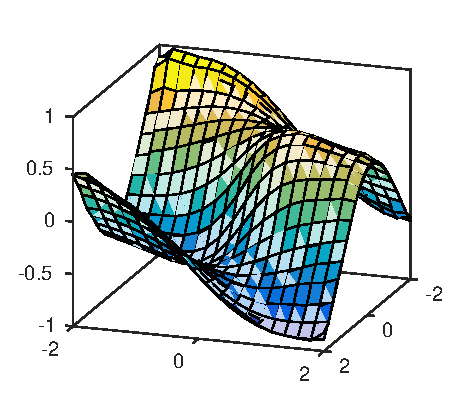
\includegraphics{plots/experiments/vdp/phi_hat.eps}
		%\caption{$\hat{W}_\varphi(t)$}
	\end{subfigure}
	\begin{subfigure}{0.5\textwidth}
		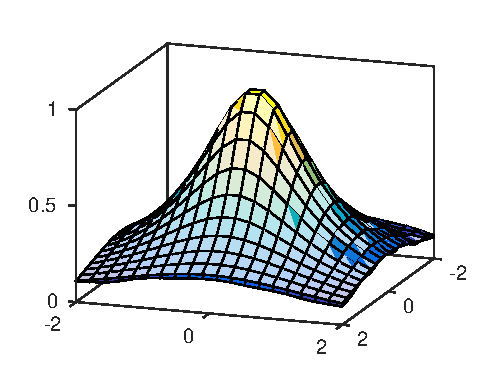
\includegraphics{plots/experiments/vdp/gamma_hat.eps}
		%\caption{$\hat{W}_\gamma(t)$)}
	\end{subfigure}
	\caption{Σύγκριση των συναρτήσεων $\varphi(x)$ (αριστερά) και $\gamma(x)$ (δεξιά) με τις προσεγγίσεις τους $\hat{\varphi}(x)$ και $\hat{\gamma}(x)$ αντίστοιχα για το πείραμα αναγνώρισης του ταλαντωτή \textit{Van Der Pol}. Με γκρι (transparent) απεικονίζονται οι πραγματικές συναρτήσεις ενώ οι χρωματισμένες επιφάνειες είναι οι προσεγγίσεις αυτών. }
	\label{fig:vdp_approximations}
\end{figure}

}

\subsubsection{Αποτελέσματα}
Χρησιμοποιώντας τις παραπάνω παραμέτρους, έγινε προσομοίωση του συστήματος κλειστού βρόγχου για $300$ περιόδους. Στο Σχήμα \ref{tab:vdp_schema_params} παρουσιάζεται η εξέλιξη κάποιων παραμέτρων των δυο νευρωνικών δικτύων. Από τα σχήματα αυτά φαίνεται πως ο χρόνος προσομοίωσης ήταν αρκετός για να σταθεροποιηθούν τα βάρη. Βλέπουμε επίσης, πως ενώ τα βάρη της $\hat{\varphi}(x)$ συγκλίνουν σε κάποιες τιμές χωρίς μεγάλες διακυμάνσεις, τα βάρη της $\hat{\gamma}(x)$ εκτελούν ταλάντωση - διαφορετικού πλάτους το κάθε ένα από αυτά - γύρω από κάποιες τιμές. Το φαινόμενο αυτό οφείλεται στην επιλογή μεγάλων κερδών $\beta_{\gamma_{ij}}$ και μπορεί να βελτιωθεί μειώνοντας τα αντίστοιχα κέρδη. Στην προκειμένη περίπτωση ωστόσο, για να αντιμετωπίσουμε το πρόβλημα αυτό, εξάγουμε τα βάρη $w_{\gamma i}$ ώς:
\begin{equation*}
	\bar{w}_{\gamma i} = mean_{t \in [t_a,t_b]} \{w_{\gamma i}(t)\}
\end{equation*}
όπου $[t_a,t_b]$ ένα επιλεγμένο χρονικό διάστημα στο οποίο τα βάρη κινούνται γύρω από μια σταθερή μέση τιμή. Στο συγκεκριμένο πείραμα χρησιμοποιείται ο μέσος όρος κατά τις δυο τελευταίες περιόδους της προσομοίωσης.

Σχετικά με την ποιότητα της προσέγγισης, στο Σχήμα \ref{fig:vdp_approximations} απεικονίζονται οι προσεγγίσεις των συναρτήσεων σε σύγκριση με τις πραγματικές, ενώ στα Σχήματα \ref{fig:vdp_phi_tilde} και \ref{fig:vdp_gamma_tilde} παρουσιάζουμε το σφάλματα $\tilde{\varphi}(x_1,x_2)$ και $\tilde{\gamma}(x_1,x_2)$ αντίστοιχα. Τέλος, στον Πίνακα \ref{tab:statistics_vdp} δίνουμε κάποια στατιστικά χαρακτηριστικά των προσεγγίσεων καθώς και της πραγματικής συνάρτησης έτσι ώστε να διευκολύνουμε την διαδικασία της αξιολόγησης αποτελεσμάτων.


\begin{table}
	\centering
	\begin{tabular}{  c | c | c | c | c | c }
		& $\min_{x \in \Omega_x}$ & $\max_{x \in \Omega_x}$ & Έυρος Τιμών & $\max(\abs{\tilde{e}})$ & Σχετικό Σφάλμα  \\ \hline \hline
		$\varphi(x)$ & $-0.8999$ & $0.8999$ & $1.7997$ & $0.1496$ & $8.31\%$ \\
		$\gamma(x)$  & $ 0.1111$ & $ 1.0$   & $0.8889$ & $0.0417$ & $4.69\%$
	\end{tabular}
	\caption{Στατιστικά στοιχειά προσεγγίσεων για τον ταλαντωτή \textit{Van Der Pol}}
	\label{tab:statistics_vdp}
	%\caption{Στατιστικά χαρακτηριστικά των προς αναγνώριση συναρτήσεων και του σφάλματος των εκτιμήσεων. (Για την συνάρτηση $f(x)g^{-1}(x)$ η μετρική \textit{NRMSE} δεν είναι ακριβής καθώς η μέση τιμή της συνάρτησης είναι ίση με το μηδέν)}
\end{table}

\begin{figure}
	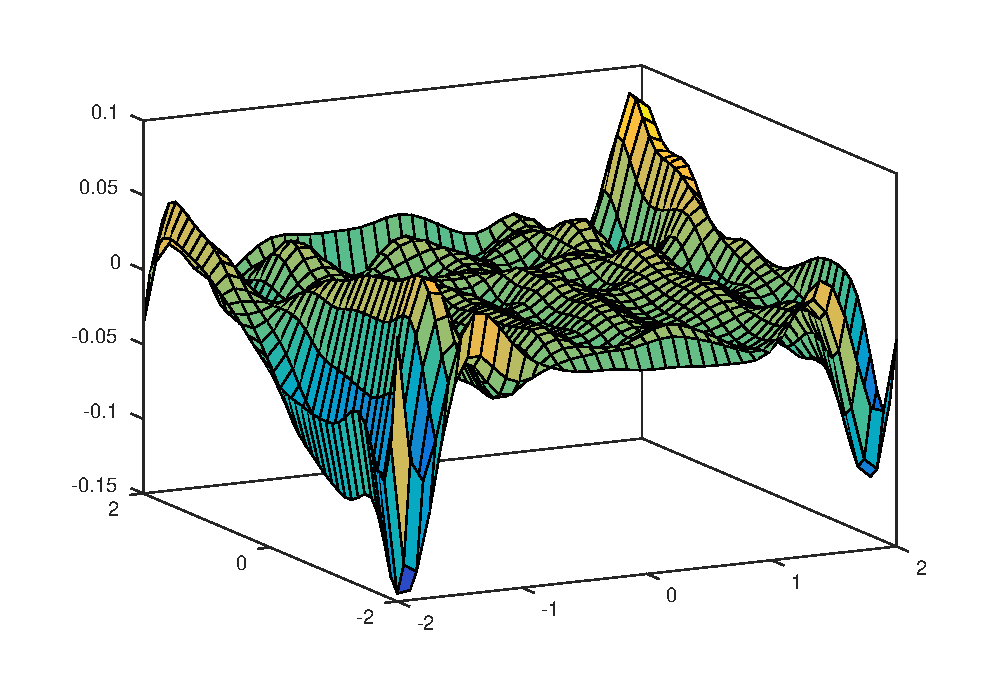
\includegraphics{plots/experiments/vdp/phi_hat_error.eps}
	\caption{Σφάλμα $\tilde{\varphi}(x)$ στο σύνολο $\Omega_x$}
	\label{fig:vdp_phi_tilde}
\end{figure}

\begin{figure}
	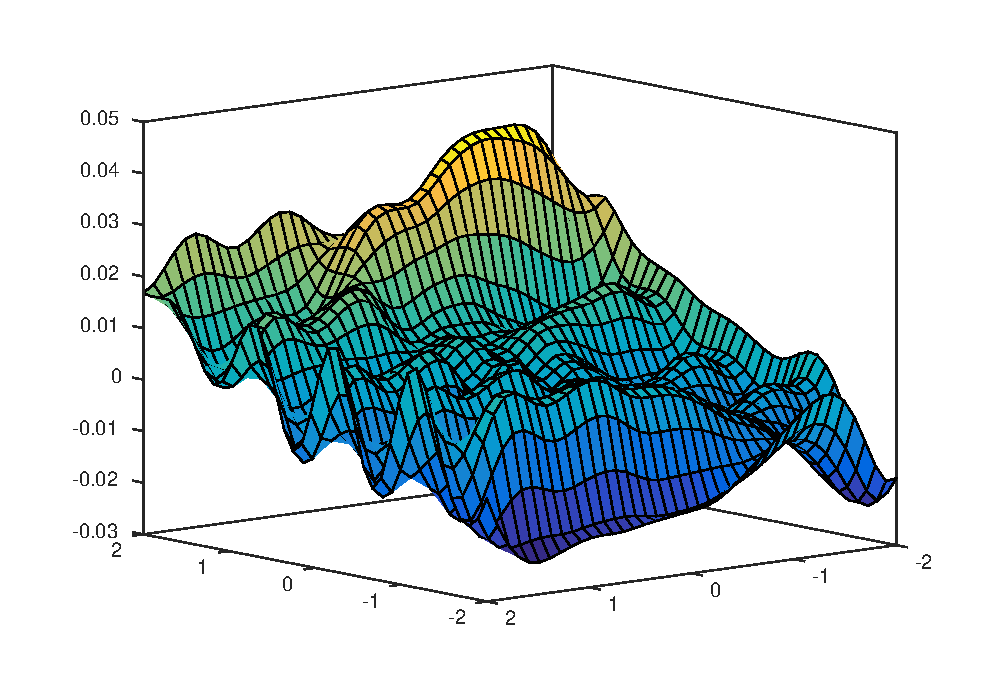
\includegraphics{plots/experiments/vdp/gamma_hat_error.eps}
	\caption{Σφάλμα $\tilde{\gamma}(x)$ στο σύνολο $\Omega_x$}
	\label{fig:vdp_gamma_tilde}
\end{figure}

Από τα παραπάνω στοιχεία οδηγούμαστε στο συμπέρασμα πως το σχήμα αναγνώρισης καταφέρνει να αναγνωρίσει επιτυχώς τις μη γραμμικότητες του  ταλαντωτή \textit{Van der Pol} παρόλο που δεν ανήκει στην κλάση συστημάτων \textit{Euler Lagrange} που μελετάμε. Κατά δεύτερον αξίζει να σημειωθεί πως μελετώντας τις γραφικές παραστάσεις \ref{fig:vdp_phi_tilde} και \ref{fig:vdp_gamma_tilde}, παρατηρούμε πως ενώ η ποιότητα των προσεγγίσεων είναι πολύ καλή στο εσωτερικό του $\Omega_x$, στο σύνορο φαίνεται πως η ποιότητα χειροτερεύει. Το αποτέλεσμα αυτό είναι αρκετά λογικό, αφού στο εσωτερικό του χώρου $\Omega_x$ υπάρχει επαρκής κάλυψη από γκαουσιανές ενώ αντίθετα τα σημεία που βρίσκονται στο σύνορο προσεγγίζονται από ένα λιγότερο πυκνό πλέγμα γκαουσιανών.


\subsection{Βραχίονας δυο βαθμών ελευθερίας}
Σε αυτό το τελευταίο πείραμα θα προσπαθήσουμε να αναγνωρίζουμε το δυναμικό σύστημα που περιγράφει την λειτουργία ενός βραχίονα δυο βαθμών ελευθερίας. Αρχικά παρουσιάζουμε τις εξισώσεις που περιγράφουν την λειτουργία του: 

\subsection{Ρομποτικός βραχίονας}
\label{exampleB}
Το τελευταίο σύστημα που θα εξετάσουμε είναι ο βραχίονας δύο βαθμών ελευθερίας, όπως παρουσιάστηκε στην εργασία\cite{bechlioulis2008robust}, ο οποίος περιγράφεται από την ακόλουθη δυναμική:
\[
M(q)\ddot q + C(q,\dot q)\dot q + g(q) = \tau,
\]
όπου $q = [q_1, q_2]$ είναι οι γωνιακές θέσεις [\si{\radian}], $\dot q$ οι γωνιακές ταχύτητες [\si{\radian/\second}], και $\ddot q$ οι γωνιακές επιταχύνσεις  [\si{\radian/\second^2}]. Ο θετικά ορισμένος πίνακας αδράνειας $M(q)$ ορίζεται ως:
\[
M(q) = \bmqty{M_{11} & M_{12}\\ M_{21} & M_{22}}
\]
με
\begin{align*}
M_{11} &= I_{Z_1} + I_{Z_2} + 0.25 m_1 \ell_1^2 
+ m_2(\ell_1^2 + 0.25 \ell_2^2 + \ell_1 \ell_2 c_2),\\
M_{12} &= M_{21} = I_{Z_2} + m_2 (0.25 \ell_2^2 + 0.5 \ell_1 \ell_2 c_2),\\
M_{22} &= I_{Z_2} + 0.25 m_2 \ell_2^2,
\end{align*}
όπου $I_{Z_1}$, $I_{Z_2}$ αναπαριστούν τις ροπές αδράνειας των συνδέσμων [\si{\kilo\gram \metre^2}], $\ell_1, \ell_2$ είναι τα μήκη τους [\si{\metre}], και $m_1$, $m_2$ οι μάζες τους [\si{\kilo\gram}]. Επιπλέον, χρησιμοποιείται ο παρακάτω συμβολισμός χάριν συντομίας:
\[\begin{array}{ll}
c_1 = \cos(q_1) & c_{12} = \cos(q_1 + q_2)\\
s_2 = \sin(q_2) & c_2 = \cos(q_2)
\end{array}\]
Ακόμη, ως $C(q, \dot q)$ συμβολίζουμε τον πίνακα που περιέχει τις δυνάμεις \textit{Coriolis}:
\[
C(q, \dot q)\dot q = \bmqty{-c \dot q_2 +  & -c(\dot q_1 + \dot q_2)\\ c \dot q_1 & 0}
\]
Με τον όρο $c$, συμβολίζουμε τον όρο $c = 0.5 m_2 \ell_1 \ell_2 s_2$ για συντομία. Επιπροσθέτως, $g(q)$ είναι το διάνυσμα των βαρυτικών ροπών:
\[
g(q) = 
\bmqty{0.5 m_1 g \ell_1 c_1 + m_2 g (\ell_1 c_1 + 0.5 \ell_2 c_{12}) \\
	0.5 m_2 g \ell_2 c_{12}}  
\]
όπου $g = 9.81 \si{\metre\per\second^2}$ είναι η βαρυτική σταθερά επιτάχυνσης. Τέλος, $\tau =[\tau_1, \tau_2]$ είναι οι ροπές [\si{\newton\metre}] οι οποίες δρουν ως είσοδοι ελέγχου. Οι ακριβείς τιμές των παραμέτρων του συστήματος αναγράφονται στον Πίνακα~\ref{tab:2dof_params}. 

Το σύστημα μπορεί εύκολα να έρθει στη μορφή~\eqref{eq:mimo_nonlinear} πολλαπλασιάζοντας από αριστερά με τον θετικά ορισμένο πίνακα $M^{-1}(q)$, καταλήγοντας στο ακόλουθο σύστημα διαφορικών εξισώσεων:
\[
\ddot q = - M^{-1}(q) \pqty{C(q,\dot q),\dot q + g(q)} + M^{-1}(q)u 
\]
Παρατηρώντας τις παραπάνω εξισώσεις εύκολα επαληθεύεται ότι το σύστημα ανήκει στην κλάση συστημάτων που μελετάμε αφού ο πίνακας $ M^{-1}(q)$ αφενός είναι θετικά ορισμένος, και αφετέρου είναι συνάρτηση μόνο των θέσεων $q_1$, $q_2$ και όχι των γωνιακών ταχυτήτων.

\begin{table}
	\centering
	\caption{Παράμετροι του συστήματος για το παράδειγμα~\ref{exampleB}}
	\label{tab:2dof_params}
	\begin{tabular}{l | ccc}
		\hline \hline
		$i$ & $m_i$ & $I_{Z_i}$ & $\ell_i$ \\ \hline \hline
		$1$ & $3.2$ & $0.96$ & $0.5$ \\\hline 
		$2$ & $2.0$ & $0.81$ & $0.4$ \\ \hline 
	\end{tabular}
\end{table}


{\begin{wraptable}{r}{0.3\textwidth}
		\centering
		\captionsetup{format=plain}
		\caption{Παράμετροι σχήματος αναγνώρισης για τον ρομποτικό βραχίονα}
		\label{tab:2dof_schema_params}
		\begin{tabular}{ l | r }
			\hline\hline
			\text{Parameter} & Value \\ \hline\hline
			$k$             & $30$   \\ \hline
			$\lambda$       & $1 $   \\ \hline
			$\beta_{\varphi} \;\text{(bias)}$     & $0.2$ \\ \hline
			$\beta_{\varphi} \;\text{(gaussian)}$ & $1$ \\ \hline
			$\beta_{\gamma} \;\text{(bias)}$     & $0.1$ \\ \hline
			$\beta_{\gamma} \;\text{(gaussian)}$ & $0.2$ \\ \hline
			$\rho_0      $ & $4$  \\ \hline
			$\rho_\infty $ & $0.02$  \\ \hline
			$l           $ & $2$  \\ \hline
			$\textit{ΔΤ} $  & $1$ 	\\ \hline \hline	
		\end{tabular}
	\end{wraptable}

\subsubsection{Σχήμα Αναγνώρισης}
Ορίζοντας το διάνυσμα καταστάσεων $x = \bmqty{q_1,\dot q_1,q_2,\dot q_2 }^T$, σκοπός της παρούσας εφαρμογής, είναι η αναγνώριση των άγνωστων συναρτήσεων
\begin{equation*}
	\Phi(x) = G^{-1}(x) f(x) = -\pqty{C(q,\dot q),\dot q + g(q)}
\end{equation*}
και 
\begin{equation*}
\Gamma(x_1, x_3) = G^{-1}(x_1, x_3) = M(q)
\end{equation*}
στο συμπαγές και κλειστό σύνολο $\Omega_x =\bmqty{-0.5,0.5}^4$. Για τον σκοπό αυτό θα χρησιμοποιήσουμε νευρωνικά δίκτυα RBF με τα  διανύσματα οπισθοδρομητών $Z_\varphi(x)$ για την αναγνώριση των συναρτήσεων του $\Phi(x)$ και $Z_\gamma(x)$ για τις συναρτήσεις του $\Gamma(x)$. Ομοίως με τα Παραδείγματα \ref{exp:wing_rock} και \ref{exp:vdp} τα κέντρα των οπισθοδρομητών επιλέγονται με τέτοιο τρόπο έτσι ώστε να καλύψουν ομοιόμορφα το σύνολο $\Omega_x$. Έτσι λοιπόν, τα κέντρα των οπιθοδρομητών $Z_\Phi(x)$ και $Z_\Gamma(x)$ τοποθετούνται στα πλέγματα
\begin{equation*}
\begin{matrix}
	\mathcal{C}_\Phi = \bigtimes\limits_{i=1}^{4}  \begin{Bmatrix}
	0 \pm  0.25 k, \quad  k = 1,2
	\end{Bmatrix}
&
\text{και}
&
\mathcal{C}_\Gamma = \bigtimes\limits_{i=1}^{2}  \begin{Bmatrix}
0 \pm  0.25 k, \quad  k = 1,2
\end{Bmatrix}
\end{matrix}
\end{equation*} 
αντίστοιχα. Στην συνέχεια επιλέγουμε τις διασπορές $\sigma$ έτσι ώστε δυο γειτονικές γκαουσιανές συναρτήσεις RBF να έχουν $75\%$ επικάλυψη, καταλήγοντας έτσι στην τιμή $\sigma = 0.2331$. Τέλος, σε κάθε προσέγγιση θα χρησιμοποιηθεί και ένας επιπλέον όρος πόλωσης (bias term). Οι υπόλοιποι παράμετροι του σχήματος αναγνώρισης παρουσιάζονται στον Πίνακα \ref{tab:2dof_schema_params}.

}

\begin{figure}
	\begin{subfigure}{0.5\textwidth}
		% This file was created by matlab2tikz.
%
\definecolor{mycolor1}{rgb}{0.00000,0.44700,0.74100}%
\definecolor{mycolor2}{rgb}{0.85000,0.32500,0.09800}%
\definecolor{mycolor3}{rgb}{0.92900,0.69400,0.12500}%
%
\begin{tikzpicture}

\begin{axis}[%
width=0.761\textwidth,
height=0.65\textwidth,
at={(0\textwidth,0\textwidth)},
scale only axis,
xmin=0,
xmax=30000,
xlabel style={font=\color{white!15!black}},
xlabel={Time, $t$},
ymin=-25,
ymax=5,
ylabel style={font=\color{white!15!black}},
ylabel={$\hat{W}_{\varphi_1} (t)$},
axis background/.style={fill=white},
xmajorgrids,
ymajorgrids
]
\addplot [color=mycolor1, line width=1.2pt, forget plot]
  table[row sep=crcr]{%
0	0\\
22.0010141601306	-11.6250756380832\\
40.006214029152	-15.1868213215675\\
58.4816655603645	-18.2310066142672\\
78.6879773681503	-19.3384505572103\\
100.575489070172	-19.7951175957132\\
123.3101701749	-20.0679332713953\\
146.228660635523	-16.3539808893911\\
172.199381604511	-17.7978798731201\\
199.216871204237	-18.9809402202627\\
226.142061781371	-19.7393703766866\\
253.772297893262	-19.8029810874032\\
282.213017586499	-19.8352434565895\\
312.89006128988	-19.9865503038491\\
347.705056364881	-20.2412509964488\\
380.612079327715	-20.2134744796167\\
405.795319896417	-19.7570380008583\\
430.056255439333	-19.8759526888171\\
458.369849905459	-20.1561375338897\\
488.768333195454	-20.1766186764326\\
513.0021832854	-19.4459834155314\\
533.191880132432	-19.1520956009044\\
554.687533079377	-19.4087430634172\\
578.451772799926	-19.9078156804571\\
603.376074201657	-20.1921009193211\\
628.00477153439	-19.8271275677471\\
649.79506491033	-18.9920706858247\\
671.834495370531	-19.2472445978819\\
696.193267098693	-19.7076777453913\\
720.364412559302	-20.0085208051787\\
749.284382873229	-20.1838666656113\\
776.20512120143	-20.069585962683\\
802.007542783762	-20.018796065382\\
831.034487188055	-20.1937623188933\\
861.011764461884	-20.229111205972\\
889.0061174537	-20.5255837098121\\
920.244393502478	-20.4966945479209\\
950.83492014186	-20.5430752320281\\
981.77304821838	-20.4253338457711\\
1011.22772520844	-20.4522919552619\\
1039	-20.3436249444494\\
1067.04456274024	-20.5006100581231\\
1097.98588926185	-20.546273315038\\
1126.78319450584	-20.3014945743635\\
1148.81605766601	-19.791506970203\\
1170.14953634024	-20.0940345173985\\
1192.34529951866	-20.2740462210713\\
1215.36345701218	-20.3969904696969\\
1239.8968705598	-20.3818163895412\\
1262.33614018248	-19.9499502013496\\
1282.68327601124	-20.0948266919004\\
1303.59919283675	-20.1762118361657\\
1352.02516904102	-20.4156484909581\\
1376.70631738191	-20.352613416595\\
1429.24933502657	-20.489135769476\\
1459.17708984501	-20.5462371747635\\
1490.00099732692	-20.4781299736569\\
1516.23387788289	-20.5636004240732\\
1550.66668012608	-20.6439725490018\\
1582.75625540383	-20.6936063195972\\
1616.81593034523	-20.5923933044942\\
1648.20604414454	-20.5574921415791\\
1676.02078559775	-20.6208344925581\\
1705.57737457926	-20.6709953978934\\
1736.39258040744	-20.5734656633358\\
1763.07560540824	-20.4156573906694\\
1785.71468998064	-20.373615911114\\
1808.05797066675	-20.5254252548766\\
1832.20716207739	-20.5948876209841\\
1857.12788227338	-20.5545620917692\\
1881.99763103162	-20.3489175392824\\
1903.76326242409	-20.3387222906058\\
1925.86568708504	-20.4226474145762\\
1949.69343372955	-20.554593696088\\
1975.51143158512	-20.6310032490219\\
2002.65543040722	-20.5227424329241\\
2029.54720384807	-20.5485251265709\\
2087.82811499125	-20.6659858386993\\
2119.21018741299	-20.6038331445525\\
2147.60974244864	-20.5812443752984\\
2179.22821710862	-20.7037765209243\\
2212.00087655821	-20.7312934301917\\
2248.27470887678	-20.627758147486\\
2275.31002342947	-20.607197063604\\
2304.04067707442	-20.7074745506434\\
2335.00461398508	-20.716520547805\\
2367.15670494568	-20.6404318790192\\
2392.07469832007	-20.5147877466115\\
2414.93507765002	-20.5434217674738\\
2438.21205209333	-20.6700549791058\\
2462.86399788344	-20.7246383711026\\
2489.54102798222	-20.6327054030226\\
2512.87867535083	-20.4543878733748\\
2535.76902775786	-20.5652452821378\\
2559.03789619781	-20.632060144093\\
2583.08717427489	-20.7136625815074\\
2610.55031994384	-20.613008429922\\
2636.31609578053	-20.5857764879111\\
2663.7054471777	-20.6189305100597\\
2692.54660604851	-20.7017823287642\\
2725	-20.7271236636261\\
2753.26802134881	-20.5533035606131\\
2783.80568827383	-20.6126203670174\\
2814.76898850397	-20.7207808229032\\
2849.73400486278	-20.7596048083215\\
2880.88097628015	-20.5761715987755\\
2909.70441151558	-20.6368093228884\\
2939.34543624319	-20.7459648152035\\
2970.07801066419	-20.7812192602323\\
3001.88819517193	-20.5488556235978\\
3025.18012683544	-20.5397020767523\\
3049.88755532052	-20.6944592120599\\
3096.00359725381	-20.8214498436027\\
3146.00685317941	-20.5420902199839\\
3168.56515246117	-20.6557524220079\\
3217.22937795712	-20.8135034120751\\
3244.95249248798	-20.6977511910154\\
3273.0046193674	-20.6282797406238\\
3300.94222580976	-20.6575568584594\\
3329.29257993141	-20.7696903150281\\
3360.82950483446	-20.6459991476295\\
3392.16392443045	-20.597915460392\\
3425.37713991607	-20.6485373536561\\
3456.05888044651	-20.7209652537276\\
3489.02087292794	-20.6296264082448\\
3551.62247646616	-20.6745098551837\\
3579.34357965102	-20.7992704971184\\
3610.37836927607	-20.6432116307988\\
3640.53774637625	-20.605924048341\\
3666.50400010544	-20.6869592865987\\
3690.46373933997	-20.7741083258443\\
3714.44523585703	-20.8119970370826\\
3740.21303904782	-20.7196166550493\\
3765.57874719471	-20.5835800805471\\
3789.5000012821	-20.6781658709879\\
3813.41854503588	-20.7536809490739\\
3838.02589677472	-20.8175224902006\\
3865.14487520794	-20.7179792021525\\
3893.08800109858	-20.6407387090367\\
3950.32685173723	-20.7505906155857\\
3980.91924208061	-20.6479978010138\\
4010.93781687778	-20.603797352418\\
4041.00742618711	-20.6638602379426\\
4074.62788696224	-20.7611226323861\\
4104.76099217656	-20.6616888144854\\
4135.52411753067	-20.6115555823344\\
4164.84363872227	-20.6797076072908\\
4191.67724116229	-20.7845018505213\\
4220.34181600386	-20.7917795530375\\
4251.88666221631	-20.5722708759713\\
4277.8975024907	-20.5982788278234\\
4302.65307642276	-20.7384174866202\\
4326.35727686555	-20.8169812341985\\
4351.12609962662	-20.8509397279086\\
4378.45967308257	-20.64039597191\\
4402.99755749093	-20.6039439998822\\
4427.18088671436	-20.6737883919523\\
4450.88992534439	-20.7921771923029\\
4475.64313726746	-20.8504420708232\\
4502.89300107902	-20.6661341916697\\
4532.11608990744	-20.6463551005181\\
4559.46164014736	-20.7183539744146\\
4588.83383393395	-20.7613104506127\\
4648.901018774	-20.6229095445742\\
4679.10286946986	-20.7080899854773\\
4708.28132625591	-20.73385750546\\
4737.59335486815	-20.6282719749433\\
4767.63086443802	-20.6239387636888\\
4822.81141342114	-20.7944597622081\\
4850.46800446488	-20.7827576756717\\
4878.99670483398	-20.6076634825622\\
4903.78169939709	-20.6382891097674\\
4928.73021140362	-20.7625383791892\\
4952.19546971423	-20.8119157908477\\
4976.5756600961	-20.8411845019691\\
5003.27888956456	-20.6405020493075\\
5028.55203787279	-20.6396362447631\\
5053.02400866113	-20.7156369455806\\
5076.86278048775	-20.7751425544702\\
5101.9766380536	-20.8111531948198\\
5129.07743266448	-20.6971333025504\\
5157.80285819941	-20.6622160904808\\
5185.91979487858	-20.7475306173837\\
5215.10248702628	-20.7756534988366\\
5275.28244402961	-20.6248580792853\\
5305.04877713639	-20.6838663732306\\
5335.23733968329	-20.7201749147171\\
5365.21927850344	-20.6562321397432\\
5395.93401645824	-20.6433751384684\\
5426.34678531726	-20.700568367607\\
5453.32913367534	-20.7904275532128\\
5481.1166906102	-20.662924130731\\
5510.08629175029	-20.5983998902666\\
5583.74501536359	-20.8290929051655\\
5609.83735346909	-20.7443050438815\\
5635.53931474248	-20.62938000336\\
5660	-20.694553972633\\
5684.00326531268	-20.7743972623575\\
5707.49671665597	-20.8331723217925\\
5733.79545157124	-20.7293150490732\\
5760.09513935152	-20.6593767074737\\
5787.50469944528	-20.6804280018659\\
5815.92577524783	-20.7727127916041\\
5844.51149746819	-20.7959975334998\\
5872.90032774283	-20.7076993876144\\
5902.03078964411	-20.5709112056866\\
5932.854312785	-20.7118737786368\\
5963.41988993171	-20.7381880526846\\
5995.06924468521	-20.6399636528986\\
6023.71360667713	-20.6447281687069\\
6053.12309724616	-20.7076612081801\\
6081.14536412859	-20.7552149513212\\
6110.75890227409	-20.6617313590359\\
6139.02088856078	-20.6217474578625\\
6190.23479392473	-20.8041838127028\\
6214.02582533636	-20.8414816244294\\
6240.42431496458	-20.7483682583443\\
6265.81609611158	-20.6363188026407\\
6289.57167888949	-20.7237518596849\\
6337.00612441976	-20.860037359831\\
6362.00058271465	-20.7344759342886\\
6387.84319157732	-20.6666661199379\\
6416.69670851818	-20.6912927000085\\
6445.91815529961	-20.7963980155073\\
6474.89482951662	-20.7914166412011\\
6502.13086356609	-20.6132495205711\\
6531.38454646943	-20.6411039860286\\
6563.00087664022	-20.73151451995\\
6595.2580995895	-20.7563775717499\\
6625.41561612354	-20.6499280421231\\
6653.52465348812	-20.6371988266474\\
6681.66633450691	-20.7215291289394\\
6709.16773213907	-20.7719709045887\\
6738.24895692791	-20.666338301733\\
6767.41654065242	-20.6302806694184\\
6794.67839846663	-20.7428853880701\\
6819.11592911143	-20.8212577004342\\
6843	-20.8725847089408\\
6870	-20.7292654997946\\
6895.64554063634	-20.6444589340317\\
6943.2747252336	-20.8151307490516\\
6967	-20.8752407829161\\
6991.90976691926	-20.7577900588658\\
7019.85454724813	-20.6602595941113\\
7049.88892602786	-20.7000470390594\\
7078.03034703268	-20.7837635933429\\
7105.0450997172	-20.6726434294724\\
7133.08220720066	-20.6094939682152\\
7165.20628767484	-20.6535131455494\\
7198.96597779813	-20.7589005988521\\
7227.8895480703	-20.7283025769138\\
7256.13586903482	-20.5775570389487\\
7315.32566513611	-20.7684531056984\\
7343.51664217019	-20.8001171976284\\
7372.81082181324	-20.6792331117504\\
7399.30890412766	-20.6520357884292\\
7425.90517858284	-20.7688602746675\\
7449.1860656328	-20.8358336440324\\
7471.24521644833	-20.8804459329513\\
7499.39294272152	-20.742173054321\\
7523.04429107055	-20.6389116693681\\
7547.18978972044	-20.7520472209508\\
7595.64356987678	-20.8788633401091\\
7620.16911782198	-20.7597658722698\\
7648.63306268269	-20.6632124472417\\
7678.28292029199	-20.708196396823\\
7706.92941380541	-20.7632988757323\\
7762.06455622318	-20.6302455161567\\
7796.11639457328	-20.6764541337361\\
7827.85215716439	-20.7580003675102\\
7855.54781153105	-20.6311413261901\\
7884.49050533435	-20.5985513656451\\
7915.04603274785	-20.6792529568629\\
7944.97459151303	-20.7881509144609\\
7970.95249232475	-20.803914821623\\
8000.20051690676	-20.6805150435575\\
8025.24128760182	-20.6536310995652\\
8050.71981864595	-20.7836827840401\\
8096.86391217875	-20.8858041419007\\
8125	-20.7312773093763\\
8150.27806551976	-20.6345466705206\\
8173.37481975988	-20.7399865621665\\
8197.71056301703	-20.8206557602462\\
8220.70994001865	-20.8770573632937\\
8245.54108682131	-20.7577545642198\\
8273.75847969247	-20.6654857003196\\
8331.00326681594	-20.7650775525763\\
8358.30361291683	-20.684470472901\\
8386.03109157838	-20.622664124865\\
8420.73851300205	-20.6793356990165\\
8452.9694793095	-20.7581224214009\\
8480.00533694809	-20.6427531945337\\
8509.1960041915	-20.5950882374345\\
8538.13866858349	-20.6811810042382\\
8568.57877024686	-20.7931428713673\\
8596.01359391017	-20.8022244156818\\
8625.2225427878	-20.6783773725183\\
8650.33557885922	-20.6511671817971\\
8674.80655530921	-20.770492441512\\
8697.67237086323	-20.8387727270565\\
8720.90601312488	-20.8821625457458\\
8748.51919023621	-20.7392255274062\\
8772.87097714111	-20.6445814007675\\
8795.86607076198	-20.7494304028369\\
8844.4928187413	-20.8735573873673\\
8869.33593743871	-20.7598870654583\\
8895.9912597712	-20.669559457001\\
8926	-20.6996730370884\\
8953.20734732295	-20.7828145767817\\
8979.93459639306	-20.6890698795214\\
9007.81729726913	-20.6144836194544\\
9040.045282482	-20.6489025120645\\
9075.52207723869	-20.7475187327836\\
9104.1511688793	-20.7330556408961\\
9132.86143558719	-20.5868930366487\\
9192.43610570643	-20.785325953897\\
9220.53578756602	-20.8003265016923\\
9249.90714044826	-20.6807201501942\\
9274.47252934429	-20.6560630200765\\
9298.8868417866	-20.7672193759681\\
9322.38171134601	-20.8430020565102\\
9345.85712704332	-20.8803424541002\\
9372.86747478923	-20.7382616822761\\
9397.15597424958	-20.6561371117859\\
9420.72352081034	-20.7487891111014\\
9445.50375354124	-20.8206455137624\\
9470.03276370854	-20.8646863260801\\
9494.72001503564	-20.7621727040678\\
9520.95048670254	-20.6699179553871\\
9551.22622921719	-20.6961351337632\\
9578.49052189168	-20.793879691857\\
9606.00653581649	-20.6698070061248\\
9634.2861894239	-20.6188314325045\\
9665.6974778227	-20.6701834608029\\
9700.10300010465	-20.7488236370191\\
9728.40748189801	-20.7276240175634\\
9757	-20.5712565206668\\
9816.70054209479	-20.7855826979539\\
9845.15192750833	-20.7969097815221\\
9873.8479973309	-20.6763701794443\\
9897.90219557842	-20.6535347895078\\
9920.89884936298	-20.7602613450144\\
9945.12089641397	-20.8272047748796\\
9967.75420076866	-20.8713183503933\\
9991.49619615414	-20.7568736185312\\
10015.6381273123	-20.6587163676013\\
10040.4748984579	-20.7421760727993\\
10065.1471262701	-20.8068872249605\\
10088.7271597519	-20.8538892168217\\
10112.4336380042	-20.7403868901456\\
10137.0002924905	-20.6744507770381\\
10166.1718921816	-20.6993872363673\\
10195.8567315288	-20.7988285522333\\
10223.5760787423	-20.7984309274434\\
10251.721081843	-20.6213561599216\\
10281.0559083679	-20.6410252168098\\
10312.9771602807	-20.733014041125\\
10345.3478862884	-20.754231744384\\
10375.3874619665	-20.6522824130734\\
10402.6362120879	-20.6144325022942\\
10431.8095810998	-20.7236342575088\\
10460.2986991755	-20.752881447821\\
10487.7856608359	-20.664414365503\\
10514.7886434181	-20.6330861719507\\
10563.1712794126	-20.8000047521455\\
10586.0005841636	-20.8471996846456\\
10633.2591140727	-20.6428892969343\\
10706.7608688401	-20.8401667372564\\
10729.9650921833	-20.7384164053401\\
10754.0603000727	-20.7001313667351\\
10782.9061608417	-20.6746018559606\\
10811.2851009249	-20.7561493346511\\
10838.8122545639	-20.7723676319438\\
10897.4814330221	-20.6460680751625\\
10928.3126833084	-20.6796059587869\\
10958.711617081	-20.7410420601227\\
10987.9799728329	-20.6354130723412\\
11017.4923231744	-20.616069319145\\
11047.7705521524	-20.7137675519225\\
11078.2020763132	-20.7952721845249\\
11105.0168981176	-20.6766052651365\\
11132.0065355145	-20.6015238218388\\
11180.837268897	-20.7701650560703\\
11204.007544266	-20.8691773690989\\
11226.8567328421	-20.8447498514433\\
11275.9122181789	-20.6512647154486\\
11299.2301155132	-20.7440525871534\\
11346.3113295137	-20.8760687996473\\
11369.9070264847	-20.75587315343\\
11396.1920568177	-20.6677404792645\\
11426.2572232203	-20.6976518632473\\
11453.8759103667	-20.8050851878761\\
11480.0011726298	-20.6834164593747\\
11507.3670018857	-20.6146649516668\\
11538.720233748	-20.6509666440288\\
11570.9466442886	-20.7718729820663\\
11600.6634840819	-20.7468632523523\\
11629.2552327251	-20.5947637748905\\
11659.0032659006	-20.6548945546019\\
11689.6948229364	-20.7688579945498\\
11718.3809448164	-20.7989113522563\\
11746.5537039263	-20.6807339818952\\
11771.215167891	-20.6446776468438\\
11796	-20.7605250875567\\
11820.3638618617	-20.8239824067823\\
11844.2096572353	-20.872020260289\\
11867.0997540751	-20.7577653012668\\
11891.9613852194	-20.658962472713\\
11916.4034631606	-20.7489250715262\\
11940.983824851	-20.8221223594919\\
11964.2687183622	-20.8536712461937\\
11987.6605741644	-20.738223770164\\
12012.5155860812	-20.6699206574085\\
12041.5983106503	-20.6948699255481\\
12070.8657044134	-20.7996717673814\\
12096.9154233274	-20.8069664310133\\
12125.438981148	-20.7126458957282\\
12154.4890639786	-20.6398548233046\\
12185.1733878168	-20.7154414888464\\
12215.0009897092	-20.73558181318\\
12246.0127866337	-20.6544755165633\\
12275.6869599745	-20.6574687762586\\
12333.4796243527	-20.7714234103587\\
12360.1718877862	-20.6634252638105\\
12387.0208345802	-20.6399732190148\\
12436.6726366018	-20.8067123183719\\
12459.9695211232	-20.8294324263115\\
12483.4328512503	-20.7599774735099\\
12508.4831068864	-20.6473802300679\\
12534.136852221	-20.7160226789492\\
12556.6862208933	-20.7637472100469\\
12580.8165474457	-20.834014449636\\
12604.5628662644	-20.7790670760405\\
12628.5285925226	-20.6906965174458\\
12658.1267128354	-20.6746308755464\\
12685.9559345771	-20.760504468115\\
12713.2828198036	-20.7778615273783\\
12770.5986287998	-20.6432803064745\\
12802.8282503582	-20.683829227175\\
12831.4493927615	-20.733863302321\\
12860.9340644743	-20.6378862196252\\
12891.0928447515	-20.6276217394952\\
12921.255739756	-20.7092286615807\\
12951.5574989548	-20.770521027549\\
12978.4998523276	-20.7689984515564\\
13005.6533107439	-20.6248713191417\\
13030.331662239	-20.6659333109965\\
13078.9713339615	-20.8695780777198\\
13102.3774084584	-20.8444664109702\\
13126.80134148	-20.6430088051711\\
13151.266115007	-20.6487019136075\\
13174.9019137353	-20.7458625284416\\
13221.9456253719	-20.8819571629028\\
13245.9125869108	-20.7581248918541\\
13275.2974756981	-20.6618739239348\\
13330.7232666123	-20.7700943523705\\
13356.5705521864	-20.669181301706\\
13383.9712257909	-20.6209052778977\\
13415.677459534	-20.6702315566072\\
13448.1312588489	-20.7584602906572\\
13477.7680655411	-20.7303440304313\\
13506.0426017832	-20.5839671644135\\
13534.0065310949	-20.6546547474609\\
13562.4580067404	-20.7600271174488\\
13590.7969318192	-20.7936795851383\\
13620.0278190022	-20.6650771339628\\
13644.9935447296	-20.6392856807543\\
13669.6292157111	-20.7498389598404\\
13693.5466780383	-20.8270648313264\\
13715.8071302804	-20.8691308448942\\
13764.1705494564	-20.6547263872344\\
13811.6959168231	-20.8098848081681\\
13834.489442061	-20.8389257162344\\
13857.4897628536	-20.7383284026873\\
13882.7349200257	-20.6581622904268\\
13911.7406837453	-20.6955935132173\\
13940.7620066004	-20.7765902107967\\
13967.7383360001	-20.7994651775844\\
13995.1684381262	-20.7086954340448\\
14025.2338670158	-20.638245040107\\
14055.7406594169	-20.7182030866534\\
14084.884685574	-20.7305463394478\\
14114.5912768317	-20.6394218563873\\
14143.4384205957	-20.6231666734166\\
14172.8056370825	-20.7129046219488\\
14201.415634691	-20.7803322788568\\
14228.5361710052	-20.768126180832\\
14256.5731685873	-20.6020144439899\\
14306.9133754123	-20.7694016731875\\
14329.5663184	-20.8375974074515\\
14353.2580536511	-20.8503117650835\\
14377.1570571788	-20.6436929769989\\
14401.8209138554	-20.6139768050562\\
14425.1169722494	-20.7445238863766\\
14471.2388082612	-20.8760159336998\\
14495.4914969554	-20.7523858173299\\
14525.1420207213	-20.6620202387967\\
14551.9577947941	-20.6774778688668\\
14580.2024648846	-20.7420649113301\\
14605.9629734741	-20.6725269713243\\
14633.6273769202	-20.6221525307337\\
14664.85934408	-20.652371600976\\
14696.5063819466	-20.7654184061867\\
14726.9783652478	-20.7127058893166\\
14755.2192682638	-20.5836335099266\\
14783.3056386544	-20.6516823572892\\
14810.9548953555	-20.7643625026685\\
14839.4735995488	-20.7699220560389\\
14868.5099101597	-20.6917094544697\\
14894.3433408788	-20.6392551722456\\
14919.6326456098	-20.7499976321487\\
14943.1590111958	-20.8262749369314\\
14965.7274326144	-20.869864492015\\
14989.3641727455	-20.7422527660419\\
15014.3294044259	-20.6542525174591\\
15038.0772052373	-20.7383829808387\\
15062.1776645775	-20.8089298036066\\
15085.3632902977	-20.8337258909087\\
15108.7433912122	-20.7441425559882\\
15133.0316545838	-20.6625700535806\\
15161.8009549125	-20.6956470252589\\
15191	-20.7807267376629\\
15219.0092411525	-20.8010641171932\\
15246.7735819563	-20.706894606792\\
15277.1352852273	-20.5817221818652\\
15307.6677756988	-20.7128647598111\\
15337.2443107477	-20.7415631422264\\
15370.0104251555	-20.6386557305123\\
15397.194967148	-20.6513138069931\\
15427.1826020863	-20.6800771527087\\
15454.0704976149	-20.8141662512171\\
15481.395200234	-20.6616888165372\\
15509.2076279008	-20.6213039847025\\
15534.1167957046	-20.6934369984156\\
15558.7139915151	-20.7835325071319\\
15581.1003785149	-20.8330040242981\\
15604.5834425486	-20.7995330152189\\
15628.8448444191	-20.6650821528419\\
15653.9347506205	-20.6796699731167\\
15677.0615609375	-20.7108535931293\\
15724.6825486649	-20.8797197678687\\
15777.020646434	-20.6072524739466\\
15804.5298903839	-20.7359433740748\\
15832.8325134945	-20.7713170030802\\
15860.0109582337	-20.6690018113986\\
15888.1557755691	-20.6342800472303\\
15952.0345566075	-20.7262363327609\\
15981.538122626	-20.6287028084262\\
16010.8065594949	-20.6003654154629\\
16070.2172722494	-20.7928732730397\\
16098.0277957288	-20.7947853800542\\
16126.785020362	-20.6000803365969\\
16151.4728139407	-20.6474353046542\\
16176.3429851375	-20.7686988450769\\
16198.3689235713	-20.8343928303475\\
16221.3721908456	-20.8782816776402\\
16245.945218859	-20.7416092260173\\
16270.5953929757	-20.657906004235\\
16294.2798193255	-20.7439863931759\\
16318.0725116342	-20.8189728987527\\
16340.67096354	-20.8760123419634\\
16364.0021891982	-20.7434272782666\\
16390.1470973242	-20.6721680439587\\
16420.8023746857	-20.7161488141901\\
16451.0556118142	-20.7763629305773\\
16477.5973141391	-20.7696497510806\\
16504.9108336506	-20.6363173886857\\
16534.5212148143	-20.6392761662646\\
16565.5304922078	-20.7517826925905\\
16598.8016180805	-20.7573902992226\\
16628.1967593287	-20.5727814593265\\
16657.1931626649	-20.6365999840818\\
16685.2023858603	-20.7362729663146\\
16712.6763810837	-20.7676044932668\\
16741.8931368275	-20.6876340732779\\
16768.8612150588	-20.6434055741702\\
16793.4788901552	-20.7515748844016\\
16816.0534819271	-20.8209121034051\\
16838.9793480109	-20.8456198472013\\
16862.9833444179	-20.7437340073593\\
16887.5265756772	-20.6584356282619\\
16911.0036784575	-20.7380188175193\\
16957.9615132919	-20.8415258792011\\
16980.9287698765	-20.7385258832546\\
17005.8539722484	-20.6613861551341\\
17035.8495352092	-20.6930123651691\\
17065.781146127	-20.7765863395252\\
17093.0068573718	-20.8016047974343\\
17121.754533053	-20.7063613611972\\
17152.2018283804	-20.5842760039486\\
17182.0594295384	-20.7077662799893\\
17213.1815621645	-20.7402508803607\\
17245.446276493	-20.6480742998574\\
17274.7984762561	-20.6445728345134\\
17303.1286475359	-20.7076574644889\\
17330.2756150421	-20.7437740657551\\
17358.2693719431	-20.6778496660045\\
17386.3975610482	-20.6285519641788\\
17411.0069076296	-20.7111536148113\\
17457.108789933	-20.8359245518041\\
17480.0842295621	-20.7703188344203\\
17505.0828694087	-20.6532703563535\\
17552.0134652983	-20.7102664215781\\
17600.0023503888	-20.8719277456003\\
17652.4554845402	-20.6199730579101\\
17680.8323722937	-20.7370663168731\\
17708.150632174	-20.7720982395731\\
17735.3185641035	-20.6630438164502\\
17763.56400634	-20.6347524590819\\
17797.016465427	-20.6845028865318\\
17827.8144537821	-20.7588332173545\\
17858	-20.6463632292616\\
17887.4075925319	-20.6138516533283\\
17917.0090322203	-20.6913103996703\\
17946.0062103847	-20.803421389508\\
17974.1691589159	-20.7995839561991\\
18002.7254676898	-20.6101443727748\\
18027.8101805291	-20.6340164437352\\
18074.2747532657	-20.836853245095\\
18096.9958707284	-20.8849275963294\\
18122.2102461317	-20.7418689695223\\
18145.9882358695	-20.6561081883156\\
18169.113120784	-20.7461841837758\\
18192.6440738411	-20.8169522593998\\
18216.0415658966	-20.8750380529491\\
18240.0021974845	-20.7464384652558\\
18266.384353786	-20.6636247981587\\
18325.0311694252	-20.7790776449801\\
18351.1122495609	-20.7758491453424\\
18378.8699457833	-20.6460680061609\\
18410.1274116481	-20.6361998264147\\
18441.1020676679	-20.7529274157896\\
18473.8987137187	-20.7583031278373\\
18503	-20.5741514525907\\
18530.9690073923	-20.6517648434237\\
18559.0378855896	-20.7422899306293\\
18586	-20.7733029987758\\
18615.5714323204	-20.6924737969421\\
18642.8464521891	-20.6360106430111\\
18668.0135147367	-20.7475924159808\\
18690.6646509274	-20.821840954457\\
18713.0048108393	-20.8476535326627\\
18737.0110628941	-20.7515442205004\\
18762	-20.6692449820657\\
18785.6569282122	-20.7359654513821\\
18808.3481800664	-20.7803730508531\\
18832.7609698958	-20.843498381113\\
18856	-20.7397793245364\\
18881.2388762852	-20.6608534139887\\
18910.3390336443	-20.6678216253749\\
18940	-20.7574208887672\\
18965.828677836	-20.797958134568\\
18995.8182342013	-20.7053092887181\\
19026.8933326186	-20.573985722971\\
19057.1404065991	-20.7067265548794\\
19087.000877914	-20.7453891251462\\
19120.1451684005	-20.6556910596701\\
19148.3710327109	-20.6354666606021\\
19177.2432220979	-20.6824383719904\\
19203.9233202104	-20.8160479855978\\
19231.6143828844	-20.6608292869096\\
19260.2175000999	-20.6150867786346\\
19285.024269758	-20.6906405482114\\
19308.7938219681	-20.7833614364063\\
19331.1211128609	-20.8335473824191\\
19354.2975650169	-20.8542744996957\\
19379.7347567497	-20.6571943264062\\
19404.7134473162	-20.676811108533\\
19427.1733183914	-20.7167067347109\\
19451.1555803121	-20.8129025242961\\
19474.8768779387	-20.8756084810557\\
19499.0321768979	-20.7562198284104\\
19527.8932173981	-20.642332828389\\
19556.8778384953	-20.7335700125041\\
19583.7140697174	-20.7733740917465\\
19611.52170378	-20.68338728862\\
19641.5831695434	-20.6342454119767\\
19675.5244845488	-20.6652921247769\\
19704.3547978078	-20.7782629467147\\
19734.1929729785	-20.6551110946129\\
19764.4646903608	-20.6148558336645\\
19823	-20.7937406735655\\
19850.1674720539	-20.7917285528893\\
19878.2830113884	-20.6083073777008\\
19903.1948038953	-20.6315775137118\\
19927.6261840254	-20.7628988239485\\
19949.7780582885	-20.839044867691\\
19972.261740706	-20.8839316322046\\
19997.9334846695	-20.7402740421167\\
20021.9134510645	-20.6657477173831\\
20067.492799671	-20.817275218109\\
20090.7017011282	-20.8751730622571\\
20114.7423141378	-20.7593181536358\\
20140.8222802608	-20.6681129552053\\
20201.2605662048	-20.7726374285885\\
20227.2832062315	-20.7596217586761\\
20255.6997318595	-20.6397028406682\\
20286.8548914897	-20.6638252653211\\
20319.2584301617	-20.7603678675077\\
20349.7580938724	-20.7616506597915\\
20379.191284371	-20.5943283175111\\
20407.8971142185	-20.6492767374984\\
20436.5504507483	-20.7657846938455\\
20464.159705265	-20.7680683574326\\
20493.6825172191	-20.6885330326804\\
20519.8580519221	-20.6417031433957\\
20544.346668614	-20.7478706783077\\
20566.7333416876	-20.8227109317777\\
20589.6154201919	-20.8587648587018\\
20613.8004751335	-20.7434172058493\\
20639.002184571	-20.6575948707978\\
20662.2431619448	-20.7472308668475\\
20684.563545512	-20.7826380792139\\
20708	-20.8421134737109\\
20730.980467321	-20.7406434961631\\
20755.6801579311	-20.6795535908714\\
20785.2384644385	-20.6686721190199\\
20815.3598074557	-20.7583652880567\\
20840.8595656164	-20.7992175122999\\
20870.7253095709	-20.7054793575262\\
20902.1612640542	-20.5832830799591\\
20931.3264340366	-20.7127563702488\\
20961.2297979928	-20.7424216402687\\
20994.0182029041	-20.6556028584819\\
21023.1906600477	-20.6376098594992\\
21052.7071308584	-20.7109314249101\\
21079.9056418274	-20.7659185984994\\
21107.0097902397	-20.6662551796835\\
21135.2546177424	-20.6141489095025\\
21182.411577734	-20.7693101679761\\
21204.3643753374	-20.8692007537575\\
21227.8168186376	-20.8533526053943\\
21253.0273905046	-20.6494330215246\\
21277.4258184752	-20.630361053536\\
21300.8074865441	-20.754936866455\\
21346.1690303694	-20.8769514806881\\
21370.1651190634	-20.7573021111348\\
21398.9066495408	-20.6681988957753\\
21455.1205657992	-20.7451943180895\\
21481.8252842627	-20.6754101042607\\
21510.6977755172	-20.6269751132932\\
21544.7947207753	-20.6759604764993\\
21575.4123758837	-20.7446939547517\\
21604.444208453	-20.718382911753\\
21635.1577173304	-20.5943033609983\\
21664.8867823646	-20.6827312687165\\
21693.3310105	-20.7919815998575\\
21720.463179188	-20.7933840682635\\
21750.1153650781	-20.6847908083437\\
21774.8078555814	-20.6543495807891\\
21798.6747108913	-20.7670704975462\\
21820.5429186501	-20.8367240242769\\
21843.1746643419	-20.8755293260074\\
21867.9277910391	-20.7563304265495\\
21892.4352381078	-20.64987674847\\
21916.6338079603	-20.7534374308671\\
21961.4078319811	-20.8581422164025\\
21985.4633600679	-20.7283073936196\\
22010.5877227452	-20.6652397028301\\
22040.4255038917	-20.6891268867403\\
22070.8935941705	-20.7999126058894\\
22097.0199964571	-20.8080447162247\\
22156.7543914165	-20.6309669656657\\
22185.8441492491	-20.7393768954098\\
22216.8052825797	-20.7595350699303\\
22278.2241326767	-20.6106076300966\\
22306.812491607	-20.7253197379432\\
22334.0260371876	-20.7786785157405\\
22361.3289898076	-20.6677338143963\\
22389.8083203582	-20.6376305745544\\
22436.2630625386	-20.7969132426952\\
22458.5658484209	-20.8435185720737\\
22482.2685834444	-20.7573948945756\\
22507.11702482	-20.6334226437175\\
22578.4741394584	-20.826069158782\\
22601.9070106313	-20.8303862737739\\
22625.6827884191	-20.7808351764579\\
22654.7638888237	-20.6670442342547\\
22684.4076349532	-20.7426550773998\\
22710.7677477311	-20.7763623901992\\
22739.4570755265	-20.6820854061625\\
22770.8230271961	-20.6391372449798\\
22801.0158882327	-20.6696905841709\\
22830.1695816702	-20.7165386161942\\
22860.2114887462	-20.6274176938641\\
22890.8544211917	-20.6286311418116\\
22949.2559566176	-20.794915281087\\
22975.8026610568	-20.7882394652806\\
23004.2401238047	-20.6344328095438\\
23029.0037727216	-20.6636961901022\\
23074.9659016501	-20.8392038444144\\
23097.5967481729	-20.8803483109223\\
23122.991354983	-20.7409453450673\\
23147.6895397034	-20.6541171179924\\
23171.3632244564	-20.7518583719138\\
23218.4158634391	-20.8795484721413\\
23241.6229597534	-20.7602134602021\\
23270.6833116223	-20.6664889445274\\
23301.4107889625	-20.6949604164511\\
23328.6613768868	-20.7967383562464\\
23355.675568748	-20.675070299254\\
23384.6414632861	-20.6218381592116\\
23415.5052193998	-20.6652146277484\\
23447.8406826391	-20.7636087223691\\
23478.0075391317	-20.7294658941901\\
23508.1229602769	-20.5885434092561\\
23536.6359696401	-20.6837057807097\\
23565.0288488763	-20.766443246619\\
23592.8510128588	-20.7936576771608\\
23622.5932477468	-20.684641548949\\
23648.2075357767	-20.6512189521563\\
23672.0823056826	-20.7750637996905\\
23716.1491956542	-20.8715049464845\\
23740.3816979341	-20.7521710480905\\
23765.8331265881	-20.6593421196631\\
23790.1410748871	-20.7433383577663\\
23837.407162001	-20.8596131398408\\
23860.8354377281	-20.7359363300893\\
23887.53541793	-20.6703596096268\\
23918.0073610901	-20.7039110866172\\
23947.3731162697	-20.797422039901\\
23975	-20.7897573747541\\
24002.9586518565	-20.6287577474795\\
24033.5991782584	-20.6462242296511\\
24064.0209349202	-20.7251587346473\\
24095.9360326805	-20.7674620403232\\
24127.5008392399	-20.5694650648111\\
24184.6464932265	-20.7377568264455\\
24212.2049268531	-20.774467767078\\
24240.6313071896	-20.6929073898973\\
24268.907801419	-20.6436585294359\\
24293	-20.747254472044\\
24315.1523071887	-20.8090854287948\\
24337.0773350261	-20.8557607803232\\
24385.7801374151	-20.6438270301915\\
24410.5756919431	-20.7352855703866\\
24458.00653137	-20.8419067116047\\
24481.3220742045	-20.7387411594282\\
24506.9021076959	-20.6469372453721\\
24536.0034689854	-20.6955611213998\\
24565.4219522983	-20.7611107915327\\
24592.2106913982	-20.7976031679318\\
24652.8079729589	-20.6096618074625\\
24681.7260128992	-20.7075999144472\\
24712.0002923403	-20.7454522842272\\
24745.0003605345	-20.6401795955135\\
24773.0877959342	-20.6399827872847\\
24830.9358139663	-20.7641198884994\\
24858.3469142109	-20.676977409792\\
24887.208792067	-20.6405905386237\\
24956.047963581	-20.8332025943855\\
24979.2248683726	-20.8543402968789\\
25004.2429782458	-20.6645705241244\\
25029.771340151	-20.678927667781\\
25077.7019424257	-20.8169675408244\\
25100.9674355449	-20.8706338426418\\
25125	-20.7593450651329\\
25154.5320696163	-20.6710131731525\\
25183.7025032475	-20.7429421499255\\
25210.847948474	-20.7772015127957\\
25239.6049397722	-20.690879131027\\
25270.8313806339	-20.6402336555111\\
25301.8811087498	-20.6474018001754\\
25331.1675345974	-20.7342700834197\\
25360.3352989627	-20.6175958794956\\
25391.0244931997	-20.6310646339189\\
25451.1912289425	-20.7840630697065\\
25477.8078372828	-20.7674121516757\\
25506.2891170132	-20.6192523381396\\
25531	-20.6872685042908\\
25554.5194624649	-20.76805658796\\
25600.1752193124	-20.8893958722329\\
25625.2483002852	-20.7431048310791\\
25650.4564802937	-20.6515310215727\\
25673.7952164675	-20.7456717469795\\
25697.8779608736	-20.8202549837551\\
25721.0755831689	-20.876462495813\\
25745	-20.7452625826081\\
25774.580193739	-20.6704546166075\\
25803.8621530794	-20.7397721651905\\
25831.734193303	-20.7648465008569\\
25888.0669005408	-20.6352502698537\\
25951.8967485151	-20.7257210713324\\
25980.5357541766	-20.6311105357854\\
26010.9434604763	-20.6122442056549\\
26041.4388677881	-20.6893708247517\\
26071.1575351125	-20.7995415835612\\
26098.9370475038	-20.7933360209463\\
26127.624095011	-20.6100953950336\\
26153.6018979174	-20.6593822924733\\
26177.6346572914	-20.7632634075599\\
26200.0057624306	-20.8372447222464\\
26222.3049998102	-20.8836629493271\\
26246.9586929644	-20.7439695845314\\
26271.8341911647	-20.6643673663311\\
26295.8163534673	-20.7530588685549\\
26342.4639506703	-20.874379710287\\
26365.9724299218	-20.7636770400641\\
26395.6226380362	-20.6691002049738\\
26426.7359452704	-20.6788682432489\\
26454.5888902532	-20.7726488576955\\
26481.9072134605	-20.6763422919685\\
26510.5455701932	-20.6370409195406\\
26542.5069271121	-20.670522776898\\
26575.2133495083	-20.7504216145426\\
26604.0226127522	-20.7318453422486\\
26634.0098008162	-20.5939429763312\\
26665.0015809298	-20.6789846865177\\
26693.1808019838	-20.7930411707566\\
26720.7454894323	-20.7999057443267\\
26776.8503592609	-20.6146952403615\\
26801.0323831903	-20.772210484487\\
26823.1594586494	-20.8360599041371\\
26845.7870082138	-20.8755075903609\\
26870.2907710787	-20.7384252166194\\
26895.4406059372	-20.6545964377256\\
26919.171338932	-20.7465525791231\\
26941.8720668448	-20.8190100322863\\
26965.2207302683	-20.8664966490469\\
26989.5983556628	-20.754632136046\\
27018.8071056121	-20.6673744876061\\
27050.3648356459	-20.6948249557609\\
27078.35238074	-20.7839798110144\\
27105.170001618	-20.6716363344276\\
27134.7631411937	-20.6241132842333\\
27165.877472868	-20.6730330202736\\
27198.5629782338	-20.7553323981119\\
27228.1004255863	-20.7288218326212\\
27258.1768927357	-20.5882170297773\\
27288.5413338939	-20.6781033490988\\
27316.8296678057	-20.7853465771477\\
27344.0437179423	-20.7960725364537\\
27374.2707254258	-20.6912576270734\\
27400.8332275664	-20.6619818170329\\
27425.2366291562	-20.7745237476884\\
27447.2756616318	-20.8410908232472\\
27470	-20.868115618865\\
27494.0279742197	-20.7494666350358\\
27518.7227640712	-20.6596386845958\\
27565.6125188648	-20.8219815736957\\
27589.2036653517	-20.854097443822\\
27613.4081425588	-20.7445626532899\\
27640.8169628065	-20.6676670675952\\
27702.2572520585	-20.760783917005\\
27729.4122386305	-20.7631673686483\\
27758.331123271	-20.6186020678142\\
27790.4253706992	-20.6552599981223\\
27823.0579402056	-20.7596997165456\\
27852.6343584113	-20.7319887388185\\
27882.2044338566	-20.576251609742\\
27941.4261939574	-20.7837716271497\\
27969.0046230115	-20.7957851131505\\
27999	-20.6782855647616\\
28025.2717268287	-20.655505639068\\
28049.5943498209	-20.7747333588595\\
28071.6079319229	-20.8418295605225\\
28094.195463607	-20.871740487848\\
28118.0138598519	-20.7569313298009\\
28141.7708540616	-20.6633167159525\\
28165.8453321901	-20.7524920114047\\
28212.8436001935	-20.8531631739206\\
28237.0048153584	-20.7442944873619\\
28263.9680157547	-20.6688235321271\\
28295.7574695805	-20.7168208893781\\
28325.9597610187	-20.7807007765696\\
28352.747122493	-20.7709686730086\\
28381.6544950095	-20.6080322211674\\
28413.1823437261	-20.6561972369127\\
28445.1861304284	-20.7601128139104\\
28475.2003821585	-20.74521863068\\
28504.67220298	-20.5880591064742\\
28534.8779283477	-20.6572610793228\\
28563.0035030778	-20.7618769315704\\
28590.2210291104	-20.7879379815131\\
28620.3163183638	-20.6746102417164\\
28647.5172895388	-20.6538726268373\\
28672.0080921273	-20.7762771578709\\
28716.8606718039	-20.87323552003\\
28740.3648696059	-20.7517289759307\\
28764.2748698522	-20.6559903649759\\
28812.4038027426	-20.8045124510754\\
28836.0018179955	-20.8535581781434\\
28860.4259457145	-20.7262341904643\\
28886.2105158271	-20.658654197814\\
28918.007374564	-20.7039623642959\\
28948.2831430226	-20.7852403117104\\
28975.2043063735	-20.7890770426166\\
29004.3464674471	-20.6502931912109\\
29035.1501329456	-20.6369208610158\\
29065.5069865179	-20.7489287947283\\
29097.0394349468	-20.763775151805\\
29127.6962994105	-20.576486851849\\
29157.1777404033	-20.635954264304\\
29185.9017541274	-20.7633342692097\\
29213.3792088113	-20.772926004709\\
29242.8578737825	-20.6891015605506\\
29270.8216166032	-20.6412783741398\\
29295.4871441048	-20.7558685964832\\
29317.8497330504	-20.821899904051\\
29340.2614827784	-20.8644136675066\\
29364.2490920195	-20.7415327237359\\
29387.5040172095	-20.6601274656314\\
29411.8391524753	-20.7510504668353\\
29435.0976476214	-20.7779805275641\\
29459.0307215136	-20.846056494709\\
29483.3547858645	-20.7444305500103\\
29508.6546911831	-20.6660636955967\\
29539.1174895516	-20.6830994193879\\
29570.0326877926	-20.779776685984\\
29596.0074511777	-20.8108050509109\\
29626.4062091932	-20.6831948831714\\
29656.4270985125	-20.6445137879491\\
29686.0137636548	-20.7428242705537\\
29715.8652035444	-20.7590761154315\\
29750.2340285162	-20.6557675800759\\
29778.9569935819	-20.6360339226048\\
29808	-20.7369253793731\\
29835.1646848751	-20.7577089865517\\
29863.8334851894	-20.6703049193457\\
29892.9633558027	-20.638734511951\\
29917.1866366721	-20.7469357561495\\
29962.1547030299	-20.8554100260953\\
29985.2265665122	-20.74063920966\\
30009.0032624117	-20.649946031037\\
};
\addplot [color=mycolor2, line width=1.2pt, forget plot]
  table[row sep=crcr]{%
0	0\\
22.0010141601306	-0.312417924738838\\
40.006214029152	-0.515703067074355\\
123.3101701749	-0.515703067074355\\
146.228660635523	-0.280245129320974\\
603.376074201657	-0.280245129320974\\
628.00477153439	0.211738319529104\\
649.79506491033	0.382101074887032\\
671.834495370531	0.438525036661304\\
749.284382873229	0.438525036661304\\
776.20512120143	0.483760119986982\\
1239.8968705598	0.483760119986982\\
1262.33614018248	0.76353436347199\\
1282.68327601124	0.794678928796202\\
1352.02516904102	0.794678928796202\\
1376.70631738191	0.83151547981106\\
1490.00099732692	0.828645837173099\\
1857.12788227338	0.828645837173099\\
1881.99763103162	0.978632670157822\\
1903.76326242409	1.00201927675516\\
1975.51143158512	1.00201927675516\\
2002.65543040722	1.03532671118955\\
2489.54102798222	1.03532671118955\\
2512.87867535083	1.11747152097814\\
2535.76902775786	1.13451496629204\\
2610.55031994384	1.13451496629204\\
2636.31609578053	1.16524429224228\\
3123.7245572495	1.16524429224228\\
3146.00685317941	1.21057980637852\\
3168.56515246117	1.22336856571201\\
3244.95249248798	1.22336856571201\\
3273.0046193674	1.25110935362318\\
3740.21303904782	1.25110935362318\\
3765.57874719471	1.27674343315448\\
3813.41854503588	1.28701513207488\\
3865.14487520794	1.28701513207488\\
3893.08800109858	1.3127061402156\\
4351.12609962662	1.3127061402156\\
4378.45967308257	1.33604409971667\\
4475.64313726746	1.33570886418966\\
4502.89300107902	1.36026735592532\\
4976.5756600961	1.36026735592532\\
5003.27888956456	1.37918179663029\\
5076.86278048775	1.37424974488749\\
5101.9766380536	1.37424974488749\\
5129.07743266448	1.39774579768346\\
5733.79545157124	1.40640837781757\\
5760.09513935152	1.4291118145884\\
6362.00058271465	1.43350673924215\\
6387.84319157732	1.45551430979322\\
6991.90976691926	1.45646553086044\\
7019.85454724813	1.47795763239628\\
7620.16911782198	1.47615655852496\\
7648.63306268269	1.49704500359076\\
8245.54108682131	1.49306075102868\\
8273.75847969247	1.51327414549451\\
8869.33593743871	1.50720813201769\\
8895.9912597712	1.52705294662883\\
9372.86747478923	1.52705294662883\\
9397.15597424958	1.51396443894555\\
9470.03276370854	1.51921669582225\\
9494.72001503564	1.51921669582225\\
9520.95048670254	1.53887976536498\\
9991.49619615414	1.53887976536498\\
10015.6381273123	1.52549565369554\\
10088.7271597519	1.53058644808334\\
10112.4336380042	1.53058644808334\\
10137.0002924905	1.55018272221059\\
10609.4964830206	1.55018272221059\\
10633.2591140727	1.53568835259284\\
10706.7608688401	1.54057572864622\\
10729.9650921833	1.54057572864622\\
10754.0603000727	1.56016319352784\\
11250.726882144	1.56016319352784\\
11275.9122181789	1.54516989346303\\
11346.3113295137	1.5497195027383\\
11369.9070264847	1.5497195027383\\
11396.1920568177	1.56913845815143\\
11867.0997540751	1.56913845815143\\
11891.9613852194	1.55323995535946\\
11964.2687183622	1.5579056147144\\
11987.6605741644	1.5579056147144\\
12012.5155860812	1.57706903769576\\
12483.4328512503	1.57706903769576\\
12508.4831068864	1.56067923095179\\
12580.8165474457	1.56524843782245\\
12604.5628662644	1.56524843782245\\
12628.5285925226	1.58424778557674\\
13102.3774084584	1.58424778557674\\
13126.80134148	1.59724424986052\\
13151.266115007	1.57123158236573\\
13245.9125869108	1.57191927757958\\
13275.2974756981	1.59093647103873\\
13739.7556463961	1.59093647103873\\
13764.1705494564	1.57333641103469\\
13834.489442061	1.57773121653372\\
13857.4897628536	1.57773121653372\\
13882.7349200257	1.59675588318714\\
14377.1570571788	1.60430519780493\\
14401.8209138554	1.58250100217992\\
14495.4914969554	1.58319822544581\\
14525.1420207213	1.60211657529362\\
14989.3641727455	1.60211657529362\\
15014.3294044259	1.58346948150211\\
15085.3632902977	1.58774206112503\\
15108.7433912122	1.58774206112503\\
15133.0316545838	1.60666365036013\\
15628.8448444191	1.61288958461955\\
15653.9347506205	1.59148672567244\\
15747.9520497777	1.59148672567244\\
15777.020646434	1.61025152813818\\
16245.945218859	1.61025152813818\\
16270.5953929757	1.59061411813309\\
16340.67096354	1.5948183195178\\
16364.0021891982	1.5948183195178\\
16390.1470973242	1.61342474072444\\
16862.9833444179	1.61342474072444\\
16887.5265756772	1.59321968775112\\
16957.9615132919	1.59738080298484\\
16980.9287698765	1.59738080298484\\
17005.8539722484	1.61604037906363\\
17505.0828694087	1.622361055699\\
17529.3514683359	1.60044346562427\\
17624.0046220503	1.60044346562427\\
17652.4554845402	1.61930946110078\\
18122.2102461317	1.61930946110078\\
18145.9882358695	1.59936276154986\\
18216.0415658966	1.60341163825433\\
18240.0021974845	1.60341163825433\\
18266.384353786	1.62247633125662\\
18737.0110628941	1.62247633125662\\
18762	1.6024445545263\\
18832.7609698958	1.60646310596712\\
18856	1.60646310596712\\
18881.2388762852	1.62556053929075\\
19379.7347567497	1.63235843609436\\
19404.7134473162	1.60988502773762\\
19499.0321768979	1.60988502773762\\
19527.8932173981	1.62870549267609\\
19997.9334846695	1.62870549267609\\
20021.9134510645	1.60856990263346\\
20227.2832062315	1.63132263615989\\
20613.8004751335	1.63132263615989\\
20639.002184571	1.61108991683068\\
20840.8595656164	1.63354675430674\\
21253.0273905046	1.63961895896136\\
21277.4258184752	1.61689246771857\\
21370.1651190634	1.61689246771857\\
21398.9066495408	1.63575744522313\\
21867.9277910391	1.63575744522313\\
21892.4352381078	1.61549365174869\\
22097.0199964571	1.63783750269431\\
22482.2685834444	1.63783750269431\\
22507.11702482	1.61755667965917\\
22601.9070106313	1.62109272288944\\
22625.6827884191	1.62109272288944\\
22654.7638888237	1.63942270633925\\
23122.991354983	1.63942270633925\\
23147.6895397034	1.61905517340347\\
23355.675568748	1.64119243955065\\
23740.3816979341	1.64119243955065\\
23765.8331265881	1.6208677901086\\
23975	1.6434465024322\\
24360.9534522977	1.6434465024322\\
24385.7801374151	1.62298473509509\\
24592.2106913982	1.64533562948782\\
25004.2429782458	1.65151942220109\\
25029.771340151	1.62838950972218\\
25125	1.62838950972218\\
25154.5320696163	1.64696031583662\\
25625.2483002852	1.64696031583662\\
25650.4564802937	1.6262914403269\\
25859.1170876986	1.64849384808258\\
26246.9586929644	1.64849384808258\\
26271.8341911647	1.62757806152149\\
26481.9072134605	1.64974328629614\\
26870.2907710787	1.64974328629614\\
26895.4406059372	1.62908376787163\\
27105.170001618	1.65117146375633\\
27494.0279742197	1.65117146375633\\
27518.7227640712	1.63054324402037\\
27729.4122386305	1.65255065850215\\
28118.0138598519	1.65255065850215\\
28141.7708540616	1.63183120831309\\
28352.747122493	1.65364467327163\\
28740.3648696059	1.65364467327163\\
28764.2748698522	1.63269792468418\\
29004.3464674471	1.65436824830249\\
29364.2490920195	1.65436824830249\\
29387.5040172095	1.63392250316247\\
29626.4062091932	1.65558861463433\\
29985.2265665122	1.65558861463433\\
30009.0032624117	1.63468137204472\\
};
\addplot [color=mycolor3, line width=1.2pt, forget plot]
  table[row sep=crcr]{%
0	0\\
22.0010141601306	-0.35905237490806\\
40.006214029152	-0.610030075542454\\
123.3101701749	-0.610030075542454\\
146.228660635523	-0.552664849587018\\
603.376074201657	-0.552664849587018\\
628.00477153439	-0.0351887806937157\\
649.79506491033	0.210832628061326\\
671.834495370531	0.281885548964055\\
749.284382873229	0.281885548964055\\
776.20512120143	0.255885436868994\\
1239.8968705598	0.255885436868994\\
1262.33614018248	0.430583591638424\\
1282.68327601124	0.447658042408875\\
1376.70631738191	0.45211833545909\\
1402.94658055512	0.421118956222926\\
1857.12788227338	0.421118956222926\\
1903.76326242409	0.461922286001936\\
2002.65543040722	0.451294471116853\\
2179.22821710862	0.449366397977428\\
2489.54102798222	0.449366397977428\\
2512.87867535083	0.42784138278148\\
3123.7245572495	0.421605566156359\\
3146.00685317941	0.379563496706396\\
3217.22937795712	0.376023132277624\\
3740.21303904782	0.373799686825805\\
3765.57874719471	0.32904769754532\\
3838.02589677472	0.324549646418745\\
4351.12609962662	0.324343215339468\\
4378.45967308257	0.28423229819964\\
4427.18088671436	0.278376475216646\\
4976.5756600961	0.279491667744878\\
5003.27888956456	0.245634355076618\\
5053.02400866113	0.238254745298036\\
5609.83735346909	0.240422003309504\\
5635.53931474248	0.208104054487194\\
5707.49671665597	0.203993823201017\\
6240.42431496458	0.207026317872078\\
6265.81609611158	0.178598037215124\\
6337.00612441976	0.174641792615148\\
6870	0.178326419812947\\
6895.64554063634	0.153018852666719\\
6967	0.149150882349204\\
7499.39294272152	0.153374702451401\\
7523.04429107055	0.13056970623802\\
7595.64356987678	0.126724001842376\\
8125	0.131432636368118\\
8150.27806551976	0.1106183625634\\
8220.70994001865	0.106842912809952\\
8748.51919023621	0.111936200613854\\
8772.87097714111	0.092975920837489\\
8844.4928187413	0.0892338293233479\\
9372.86747478923	0.0946654856779787\\
9397.15597424958	0.0770434173027752\\
9470.03276370854	0.073314188317454\\
10015.6381273123	0.0627351121474931\\
10112.4336380042	0.0590382928494364\\
10166.1718921816	0.0650680291037133\\
10609.4964830206	0.0650680291037133\\
10633.2591140727	0.0499343334995501\\
10729.9650921833	0.0462626780499704\\
10782.9061608417	0.0524821643084579\\
11250.726882144	0.0524821643084579\\
11299.2301155132	0.0345581876645156\\
12483.4328512503	0.0303117565745197\\
12534.136852221	0.0138480513705872\\
13739.7556463961	0.0115509683455457\\
13788.1842489238	-0.00360363830623101\\
14989.3641727455	-0.00432178494156688\\
15038.0772052373	-0.0186109245078114\\
16270.5953929757	-0.0281535123649519\\
16364.0021891982	-0.0315796490940556\\
16420.8023746857	-0.0242153187500662\\
16887.5265756772	-0.0340433124802075\\
16980.9287698765	-0.0375027793488698\\
17035.8495352092	-0.0300984017922019\\
17505.0828694087	-0.0297108963204664\\
17529.3514683359	-0.0429663347713358\\
19379.7347567497	-0.0439141923598072\\
19404.7134473162	-0.0575191744901531\\
21253.0273905046	-0.0562739355918893\\
21277.4258184752	-0.0698513370589353\\
27518.7227640712	-0.0953469702981238\\
27613.4081425588	-0.0986526400629373\\
27672.814612462	-0.0902953145377978\\
28764.2748698522	-0.0993779510026798\\
28860.4259457145	-0.102689434344938\\
28918.007374564	-0.0942613391271152\\
30009.0032624117	-0.103088002462755\\
};
\end{axis}
\end{tikzpicture}%
		%\caption{$\hat{W}_\varphi(t)$}
	\end{subfigure}
	\begin{subfigure}{0.5\textwidth}
		% This file was created by matlab2tikz.
%
\definecolor{mycolor1}{rgb}{0.00000,0.44700,0.74100}%
\definecolor{mycolor2}{rgb}{0.85000,0.32500,0.09800}%
\definecolor{mycolor3}{rgb}{0.92900,0.69400,0.12500}%
%
\begin{tikzpicture}

\begin{axis}[%
width=0.761\textwidth,
height=0.65\textwidth,
at={(0\textwidth,0\textwidth)},
scale only axis,
xmin=0,
xmax=30000,
xlabel style={font=\color{white!15!black}},
xlabel={Time, $t$},
ymin=-0.5,
ymax=3,
ylabel style={font=\color{white!15!black}},
ylabel={$\hat{W}_{\gamma_{11}} (t)$},
axis background/.style={fill=white},
xmajorgrids,
ymajorgrids
]
\addplot [color=mycolor1, line width=1.2pt, forget plot]
  table[row sep=crcr]{%
0	0\\
22.0010141601306	1.33620324729054\\
40.006214029152	1.94506876901505\\
58.4816655603645	2.25052123505156\\
78.6879773681503	2.64746859972729\\
100.575489070172	2.612298679589\\
123.3101701749	2.73383489918706\\
146.228660635523	2.00993264494537\\
172.199381604511	1.95709862899821\\
199.216871204237	2.0744386695842\\
226.142061781371	2.40868397178929\\
253.772297893262	2.15840531550566\\
282.213017586499	2.15618423538399\\
312.89006128988	2.10103120912754\\
347.705056364881	2.24430432921872\\
380.612079327715	2.28012010437669\\
405.795319896417	2.34638471990911\\
430.056255439333	2.27174876560821\\
458.369849905459	2.16644201150848\\
488.768333195454	2.33987047767005\\
513.0021832854	2.31245495214171\\
533.191880132432	2.31496521138615\\
554.687533079377	2.33927749259601\\
578.451772799926	2.22136062649588\\
603.376074201657	2.29118876920256\\
628.00477153439	2.32503283415281\\
649.79506491033	2.42657604585838\\
696.193267098693	2.32937716893503\\
720.364412559302	2.29954962929332\\
749.284382873229	2.33926407833133\\
776.20512120143	2.35483854407721\\
802.007542783762	2.33041915704598\\
831.034487188055	2.35390013132928\\
861.011764461884	2.35138989713596\\
889.0061174537	2.33971059514806\\
920.244393502478	2.40472511756525\\
950.83492014186	2.4246156690424\\
981.77304821838	2.41581001038503\\
1011.22772520844	2.32912732452314\\
1039	2.37521645457309\\
1067.04456274024	2.40068314644304\\
1097.98588926185	2.40916451496378\\
1126.78319450584	2.33585145057805\\
1170.14953634024	2.40756568087818\\
1192.34529951866	2.38945672761838\\
1215.36345701218	2.39011681886768\\
1239.8968705598	2.42699697030548\\
1262.33614018248	2.42082023933835\\
1282.68327601124	2.40856835283194\\
1303.59919283675	2.41304790814684\\
1327.34096635567	2.42071919018417\\
1352.02516904102	2.4056446817267\\
1376.70631738191	2.37072613243072\\
1402.94658055512	2.45248228159471\\
1429.24933502657	2.42823318735464\\
1459.17708984501	2.44274687956568\\
1490.00099732692	2.44942572781292\\
1516.23387788289	2.41706438629262\\
1550.66668012608	2.47405695576163\\
1582.75625540383	2.47299352376285\\
1616.81593034523	2.48017740850992\\
1648.20604414454	2.43987453125737\\
1676.02078559775	2.42774569927133\\
1705.57737457926	2.48780608685047\\
1736.39258040744	2.48928401012745\\
1763.07560540824	2.43990793931152\\
1785.71468998064	2.45273729076507\\
1808.05797066675	2.43953002080889\\
1832.20716207739	2.46083717952934\\
1857.12788227338	2.4871630184316\\
1881.99763103162	2.47350280168394\\
1903.76326242409	2.51071293304267\\
1925.86568708504	2.48685320221921\\
1949.69343372955	2.48919900903638\\
1975.51143158512	2.49036932188028\\
2002.65543040722	2.47316562006381\\
2029.54720384807	2.52936390951436\\
2058.40404100144	2.47631084399109\\
2087.82811499125	2.50267915193035\\
2119.21018741299	2.5065832965156\\
2147.60974244864	2.49190879211164\\
2179.22821710862	2.49892404484854\\
2212.00087655821	2.51988954691842\\
2248.27470887678	2.51917005365613\\
2275.31002342947	2.49895918127368\\
2304.04067707442	2.50207527618113\\
2335.00461398508	2.49132959268536\\
2367.15670494568	2.5376556650117\\
2392.07469832007	2.49664623378339\\
2414.93507765002	2.51183424001647\\
2438.21205209333	2.4952252177136\\
2462.86399788344	2.49966999411117\\
2489.54102798222	2.54003515200748\\
2512.87867535083	2.5286028695009\\
2535.76902775786	2.53367285610511\\
2559.03789619781	2.52194918804162\\
2583.08717427489	2.5319563903322\\
2610.55031994384	2.53169483284\\
2636.31609578053	2.51687938375471\\
2663.7054471777	2.54084841432996\\
2692.54660604851	2.54778876651835\\
2725	2.53797508922798\\
2753.26802134881	2.52318824283429\\
2783.80568827383	2.53718692105031\\
2814.76898850397	2.53588012186083\\
2849.73400486278	2.54780049532928\\
2880.88097628015	2.5091651440307\\
2909.70441151558	2.53729196799395\\
2939.34543624319	2.53655679408257\\
2970.07801066419	2.54560485894035\\
3001.88819517193	2.53329897755975\\
3025.18012683544	2.54530183209863\\
3049.88755532052	2.56433416579966\\
3072.70264648159	2.54078244990524\\
3096.00359725381	2.5451280452362\\
3123.7245572495	2.58549070448498\\
3146.00685317941	2.58185703331401\\
3168.56515246117	2.58600215052502\\
3192.17104143348	2.5800516136369\\
3217.22937795712	2.56873495910622\\
3244.95249248798	2.59552670005723\\
3273.0046193674	2.59708686462545\\
3300.94222580976	2.5803293697245\\
3329.29257993141	2.57974252964777\\
3360.82950483446	2.5926562754903\\
3392.16392443045	2.55838739844694\\
3425.37713991607	2.59683011217203\\
3456.05888044651	2.60270388997378\\
3489.02087292794	2.61176046351829\\
3520.98328634123	2.57296785651488\\
3551.62247646616	2.55961957114778\\
3579.34357965102	2.56622452208103\\
3610.37836927607	2.60689743063631\\
3640.53774637625	2.57444630053942\\
3666.50400010544	2.59808048625564\\
3690.46373933997	2.56750278923573\\
3714.44523585703	2.58591804430034\\
3740.21303904782	2.5927677598047\\
3765.57874719471	2.6160225360145\\
3789.5000012821	2.62591046749731\\
3813.41854503588	2.6204790179072\\
3838.02589677472	2.60575822669853\\
3865.14487520794	2.60504048818984\\
3893.08800109858	2.61529156373217\\
3922.48070699275	2.63423719042476\\
3950.32685173723	2.63259384390403\\
3980.91924208061	2.65569992161909\\
4010.93781687778	2.57896178265582\\
4041.00742618711	2.61229774660751\\
4074.62788696224	2.61687308071487\\
4104.76099217656	2.6167305756062\\
4135.52411753067	2.58364816652102\\
4164.84363872227	2.60773390206305\\
4191.67724116229	2.61693413965986\\
4220.34181600386	2.61374652889572\\
4251.88666221631	2.61561100058316\\
4277.8975024907	2.64265600929866\\
4302.65307642276	2.60965069484155\\
4326.35727686555	2.61335316033365\\
4351.12609962662	2.60861252555696\\
4378.45967308257	2.68495967361014\\
4402.99755749093	2.65897900371056\\
4427.18088671436	2.63816891295573\\
4450.88992534439	2.6524907042658\\
4475.64313726746	2.65594592108391\\
4532.11608990744	2.65146011473553\\
4559.46164014736	2.64226700901418\\
4588.83383393395	2.65889899804097\\
4618.92862381508	2.66679398319684\\
4648.901018774	2.65493774288552\\
4679.10286946986	2.6453774008769\\
4708.28132625591	2.65694262617035\\
4737.59335486815	2.6839771331106\\
4767.63086443802	2.64331065347506\\
4796.09506777138	2.653167136501\\
4822.81141342114	2.64924149071521\\
4850.46800446488	2.66483663468534\\
4878.99670483398	2.65147112879276\\
4903.78169939709	2.67726376250721\\
4928.73021140362	2.65384570934839\\
4952.19546971423	2.64868883889358\\
4976.5756600961	2.62687758470202\\
5003.27888956456	2.70819296991613\\
5028.55203787279	2.69826102029765\\
5053.02400866113	2.6701638448576\\
5076.86278048775	2.66911783937394\\
5101.9766380536	2.66188294538733\\
5129.07743266448	2.67692091364006\\
5157.80285819941	2.67589149867126\\
5185.91979487858	2.68601433588265\\
5215.10248702628	2.67347632677411\\
5244.87984160361	2.69591601009961\\
5275.28244402961	2.68003300132477\\
5305.04877713639	2.69952604718128\\
5335.23733968329	2.66347456792937\\
5365.21927850344	2.67030174889442\\
5395.93401645824	2.67059341483036\\
5426.34678531726	2.66239754587878\\
5453.32913367534	2.65978685573646\\
5481.1166906102	2.72929103177739\\
5510.08629175029	2.67020060553841\\
5534.71107337832	2.67973084795449\\
5560.00225549118	2.66783461041268\\
5583.74501536359	2.68116451312017\\
5609.83735346909	2.684713674862\\
5635.53931474248	2.71194212817863\\
5660	2.71158107035808\\
5684.00326531268	2.70257641852731\\
5707.49671665597	2.70075149094555\\
5733.79545157124	2.73063859194372\\
5760.09513935152	2.68598032699811\\
5787.50469944528	2.70158966466624\\
5815.92577524783	2.71489567103345\\
5844.51149746819	2.70889461351544\\
5872.90032774283	2.71605644808733\\
5902.03078964411	2.67545711353523\\
5932.854312785	2.70184057088409\\
5963.41988993171	2.70810463872476\\
5995.06924468521	2.73215002426878\\
6023.71360667713	2.7154670078562\\
6053.12309724616	2.69596126916076\\
6081.14536412859	2.71413213794949\\
6110.75890227409	2.73117503436515\\
6139.02088856078	2.70732180013874\\
6165.02656000227	2.70839135791175\\
6190.23479392473	2.68597901732937\\
6214.02582533636	2.69889739374048\\
6240.42431496458	2.72506181650169\\
6265.81609611158	2.71098426864774\\
6289.57167888949	2.73854279714214\\
6313.49470315636	2.73742029541972\\
6337.00612441976	2.71774368797924\\
6362.00058271465	2.7445581176944\\
6387.84319157732	2.71576921426094\\
6416.69670851818	2.73314064113583\\
6445.91815529961	2.73713573794521\\
6474.89482951662	2.71847951092423\\
6502.13086356609	2.70240617589661\\
6531.38454646943	2.70830664757887\\
6563.00087664022	2.7215812304712\\
6595.2580995895	2.71341670652691\\
6653.52465348812	2.73351462532082\\
6709.16773213907	2.7193265828173\\
6738.24895692791	2.7691466003489\\
6767.41654065242	2.72953883545415\\
6794.67839846663	2.73391957413696\\
6819.11592911143	2.7217317636896\\
6843	2.71683060351279\\
6870	2.75242159217669\\
6895.64554063634	2.75651969435057\\
6943.2747252336	2.75743904712363\\
6967	2.73734271384819\\
6991.90976691926	2.76475362608471\\
7019.85454724813	2.75016883751232\\
7049.88892602786	2.76098288460344\\
7078.03034703268	2.74265825000475\\
7105.0450997172	2.75371570909556\\
7165.20628767484	2.72545791230732\\
7198.96597779813	2.75230607798949\\
7227.8895480703	2.74791781172826\\
7256.13586903482	2.71872815181632\\
7286.07878349411	2.73749323598895\\
7315.32566513611	2.73725729573925\\
7343.51664217019	2.74693490389473\\
7372.81082181324	2.77690227757193\\
7425.90517858284	2.73442190588685\\
7449.1860656328	2.74473518656305\\
7471.24521644833	2.73699602978741\\
7499.39294272152	2.7687402824231\\
7523.04429107055	2.78953816440844\\
7547.18978972044	2.77630440375651\\
7571.36515524789	2.77911870477328\\
7595.64356987678	2.75411719550539\\
7620.16911782198	2.74283384527735\\
7648.63306268269	2.79036095534684\\
7678.28292029199	2.75930241971582\\
7706.92941380541	2.77549585065572\\
7734.09512718724	2.77788191457876\\
7762.06455622318	2.74088796241631\\
7796.11639457328	2.75763521697809\\
7827.85215716439	2.75738632244611\\
7855.54781153105	2.81583521907669\\
7884.49050533435	2.74804558901451\\
7915.04603274785	2.75228244475875\\
7944.97459151303	2.76580685751105\\
8000.20051690676	2.76212079678953\\
8025.24128760182	2.7595597426407\\
8050.71981864595	2.78266833182352\\
8073.4108273489	2.7621990631269\\
8096.86391217875	2.75466134755698\\
8125	2.77989563860319\\
8150.27806551976	2.80484131581397\\
8173.37481975988	2.79337113445581\\
8197.71056301703	2.7957788328531\\
8220.70994001865	2.76324997376287\\
8245.54108682131	2.79260352395795\\
8273.75847969247	2.80800612531675\\
8303.01769658209	2.78007178646294\\
8358.30361291683	2.80986694716194\\
8386.03109157838	2.75233851633675\\
8420.73851300205	2.75046652977471\\
8452.9694793095	2.77262141778556\\
8480.00533694809	2.80352525429771\\
8509.1960041915	2.76083210858633\\
8538.13866858349	2.76666532764648\\
8568.57877024686	2.78238577575758\\
8596.01359391017	2.77928625187269\\
8625.2225427878	2.78705567763973\\
8650.33557885922	2.78536568412528\\
8674.80655530921	2.78916341943477\\
8697.67237086323	2.77689371521046\\
8720.90601312488	2.76868364020629\\
8748.51919023621	2.80913141405108\\
8772.87097714111	2.82246412769746\\
8795.86607076198	2.7981231330341\\
8820.25158874039	2.80169955224119\\
8844.4928187413	2.78710926939311\\
8869.33593743871	2.8141140759617\\
8895.9912597712	2.8010032031234\\
8926	2.7919165735766\\
8953.20734732295	2.78605923103169\\
8979.93459639306	2.79627711884677\\
9007.81729726913	2.78954220546075\\
9040.045282482	2.78515675120434\\
9075.52207723869	2.80757067701052\\
9104.1511688793	2.78274117897672\\
9132.86143558719	2.77178719943913\\
9192.43610570643	2.79708604819461\\
9220.53578756602	2.78477594331343\\
9249.90714044826	2.80156278588765\\
9274.47252934429	2.80295397249211\\
9298.8868417866	2.8059406304601\\
9345.85712704332	2.77651628591411\\
9372.86747478923	2.82410652676481\\
9397.15597424958	2.83342114223706\\
9420.72352081034	2.80611934831904\\
9445.50375354124	2.81731115161529\\
9470.03276370854	2.80049519526801\\
9494.72001503564	2.82742460176451\\
9520.95048670254	2.81432694630712\\
9551.22622921719	2.80337868562128\\
9578.49052189168	2.80773540796145\\
9606.00653581649	2.84886770670346\\
9634.2861894239	2.80998571405507\\
9665.6974778227	2.77947161029806\\
9700.10300010465	2.80845332533499\\
9728.40748189801	2.80549634658746\\
9757	2.783155979203\\
9785.62921761515	2.79199078938836\\
9816.70054209479	2.81017211672588\\
9845.15192750833	2.77532835516104\\
9873.8479973309	2.83297120606585\\
9897.90219557842	2.81509088670282\\
9920.89884936298	2.80973211804303\\
9945.12089641397	2.78832390001116\\
9967.75420076866	2.79457275382083\\
9991.49619615414	2.82871220269953\\
10015.6381273123	2.83491604270966\\
10040.4748984579	2.82759723132767\\
10065.1471262701	2.81897646776997\\
10088.7271597519	2.81771731382105\\
10112.4336380042	2.83824353776436\\
10137.0002924905	2.81935935538422\\
10166.1718921816	2.82559086579204\\
10195.8567315288	2.82757951581516\\
10223.5760787423	2.819238117434\\
10251.721081843	2.78004346367743\\
10281.0559083679	2.79469307665568\\
10312.9771602807	2.81844677605477\\
10345.3478862884	2.81491737188844\\
10375.3874619665	2.81577410389218\\
10402.6362120879	2.81054975666484\\
10431.8095810998	2.81771377259065\\
10460.2986991755	2.80153703446194\\
10487.7856608359	2.85961205645435\\
10514.7886434181	2.81766751904433\\
10538.8136443695	2.82240577097764\\
10586.0005841636	2.80070431712011\\
10609.4964830206	2.82431105329306\\
10633.2591140727	2.84548803100915\\
10659.0853612957	2.84287310160653\\
10682.7111748813	2.84416766273716\\
10706.7608688401	2.83088082421455\\
10754.0603000727	2.8381560279413\\
10782.9061608417	2.82383916377148\\
10811.2851009249	2.84426400245138\\
10838.8122545639	2.83829624105056\\
10866.9759553354	2.85094661814583\\
10897.4814330221	2.83917586674943\\
10928.3126833084	2.82360353708282\\
10958.711617081	2.83131517344009\\
10987.9799728329	2.86576441894067\\
11017.4923231744	2.82803010096541\\
11047.7705521524	2.82951476025119\\
11078.2020763132	2.80784920174119\\
11105.0168981176	2.85348300037731\\
11132.0065355145	2.83498797791617\\
11156.1865977248	2.83229104602287\\
11180.837268897	2.82355024494973\\
11204.007544266	2.79863139650843\\
11226.8567328421	2.81056336135953\\
11250.726882144	2.86986807277208\\
11275.9122181789	2.8514045585398\\
11299.2301155132	2.85372258914504\\
11323.7960983586	2.85902279752918\\
11346.3113295137	2.83208647202264\\
11369.9070264847	2.85887793254005\\
11396.1920568177	2.84693455991146\\
11426.2572232203	2.83538235121159\\
11453.8759103667	2.82119223644258\\
11480.0011726298	2.84538066011737\\
11507.3670018857	2.83584429945404\\
11538.720233748	2.8222097536418\\
11570.9466442886	2.84372173287193\\
11600.6634840819	2.86019013333862\\
11629.2552327251	2.84588092624108\\
11659.0032659006	2.82850013565985\\
11689.6948229364	2.83589497524008\\
11718.3809448164	2.83595739976954\\
11746.5537039263	2.87055634969875\\
11771.215167891	2.83605308413462\\
11796	2.84031510348359\\
11820.3638618617	2.83064859257138\\
11844.2096572353	2.82370706470465\\
11867.0997540751	2.85740327880194\\
11891.9613852194	2.87213041952054\\
11916.4034631606	2.85942691170931\\
11940.983824851	2.86503440763772\\
11964.2687183622	2.84536153166118\\
11987.6605741644	2.86691014417374\\
12012.5155860812	2.84572991697132\\
12070.8657044134	2.85770713644524\\
12125.438981148	2.84074474700174\\
12154.4890639786	2.85192206291686\\
12185.1733878168	2.8382943936449\\
12215.0009897092	2.84787903318647\\
12246.0127866337	2.87581763013804\\
12275.6869599745	2.85780219308072\\
12304.7055308943	2.86415427899919\\
12333.4796243527	2.84509827386864\\
12360.1718877862	2.84165164516526\\
12387.0208345802	2.85281955744722\\
12411.6367051249	2.85130598935939\\
12436.6726366018	2.84196480911123\\
12459.9695211232	2.82671629339893\\
12483.4328512503	2.8668870976071\\
12508.4831068864	2.87329765950562\\
12534.136852221	2.86809277078646\\
12556.6862208933	2.87936217107926\\
12580.8165474457	2.84563372338744\\
12604.5628662644	2.80451208371232\\
12628.5285925226	2.87348707577621\\
12658.1267128354	2.84643006147962\\
12685.9559345771	2.87151597089178\\
12713.2828198036	2.86038207375168\\
12740.1682852228	2.84170887976143\\
12770.5986287998	2.83958804891154\\
12802.8282503582	2.85201514366781\\
12831.4493927615	2.86570346059307\\
12860.9340644743	2.89813323367707\\
12891.0928447515	2.85351609605277\\
12921.255739756	2.85034382324011\\
12951.5574989548	2.82887240950367\\
12978.4998523276	2.84808820812032\\
13005.6533107439	2.87390522044734\\
13030.331662239	2.87433118739864\\
13055.5290164713	2.855712664561\\
13078.9713339615	2.82235156508614\\
13102.3774084584	2.83726007875521\\
13126.80134148	2.8774279524514\\
13151.266115007	2.86940780481746\\
13174.9019137353	2.87336559151663\\
13199.1301084555	2.88268981967849\\
13221.9456253719	2.85595079220366\\
13245.9125869108	2.87797035864423\\
13275.2974756981	2.88281498806828\\
13303.2383107863	2.85989995787531\\
13330.7232666123	2.87805775679226\\
13356.5705521864	2.90607007405924\\
13383.9712257909	2.86319630809885\\
13415.677459534	2.83318541050539\\
13448.1312588489	2.8658187279616\\
13477.7680655411	2.86139700187778\\
13506.0426017832	2.84096957048314\\
13562.4580067404	2.85886472454513\\
13590.7969318192	2.84301673658774\\
13620.0278190022	2.89456564922875\\
13644.9935447296	2.86319903931144\\
13669.6292157111	2.86188265962119\\
13693.5466780383	2.85485818391317\\
13715.8071302804	2.830265315406\\
13739.7556463961	2.87895245619075\\
13764.1705494564	2.89293988938152\\
13788.1842489238	2.88290168378444\\
13811.6959168231	2.88948992096266\\
13834.489442061	2.8633035236453\\
13857.4897628536	2.89865884244864\\
13882.7349200257	2.87806630079649\\
13911.7406837453	2.8687489922886\\
13967.7383360001	2.86998440957541\\
13995.1684381262	2.84287186316578\\
14025.2338670158	2.86948519751604\\
14055.7406594169	2.87842051586631\\
14084.884685574	2.84545872188755\\
14114.5912768317	2.8983595819227\\
14143.4384205957	2.86617149220911\\
14172.8056370825	2.86476748506539\\
14201.415634691	2.84309527235382\\
14228.5361710052	2.8605816225936\\
14256.5731685873	2.8750810242891\\
14281.3875404111	2.87020809781461\\
14306.9133754123	2.86237640554828\\
14329.5663184	2.8271127071821\\
14353.2580536511	2.84224467764216\\
14377.1570571788	2.91063942166511\\
14401.8209138554	2.87187633488793\\
14449.1645716421	2.89455330832789\\
14471.2388082612	2.86554243718274\\
14495.4914969554	2.88540489676234\\
14525.1420207213	2.89362601901303\\
14551.9577947941	2.86466665621992\\
14580.2024648846	2.88606950458416\\
14605.9629734741	2.91523123573643\\
14633.6273769202	2.87216813628766\\
14664.85934408	2.86146084096981\\
14696.5063819466	2.87782946471998\\
14726.9783652478	2.86560234919671\\
14755.2192682638	2.89707637493484\\
14783.3056386544	2.85421821014097\\
14810.9548953555	2.87472070568765\\
14839.4735995488	2.87248329054637\\
14868.5099101597	2.90565437165787\\
14894.3433408788	2.87424304258093\\
14919.6326456098	2.87250875546306\\
14943.1590111958	2.86606239305547\\
14965.7274326144	2.84425627033124\\
14989.3641727455	2.89146342146341\\
15014.3294044259	2.90289465884416\\
15038.0772052373	2.89266200484053\\
15062.1776645775	2.90039748202616\\
15085.3632902977	2.8658333004023\\
15108.7433912122	2.90862723633472\\
15133.0316545838	2.88389554409878\\
15161.8009549125	2.87849943864785\\
15191	2.89542560337213\\
15219.0092411525	2.88005763215915\\
15246.7735819563	2.89784009331197\\
15277.1352852273	2.85689890409776\\
15307.6677756988	2.87869172079081\\
15337.2443107477	2.88198637184178\\
15370.0104251555	2.91764035728556\\
15397.194967148	2.88772962070288\\
15427.1826020863	2.86388322009225\\
15454.0704976149	2.84564601074817\\
15481.395200234	2.927312712618\\
15509.2076279008	2.87289520567356\\
15534.1167957046	2.87465633894317\\
15558.7139915151	2.87041155411134\\
15581.1003785149	2.8586278339244\\
15604.5834425486	2.82802842558158\\
15628.8448444191	2.934505443136\\
15653.9347506205	2.90628713676415\\
15677.0615609375	2.87719485206253\\
15701.4247928756	2.8779658166568\\
15724.6825486649	2.87210363845224\\
15747.9520497777	2.901116377383\\
15777.020646434	2.87300920223061\\
15804.5298903839	2.89526724189272\\
15860.0109582337	2.87880513978598\\
15888.1557755691	2.86820975251612\\
15920.8917272547	2.87234388071738\\
15952.0345566075	2.86568965689003\\
15981.538122626	2.93336165444998\\
16010.8065594949	2.84495602365496\\
16041.0255862117	2.87620891728147\\
16070.2172722494	2.86769197929971\\
16098.0277957288	2.86987786220925\\
16126.785020362	2.88067402372326\\
16151.4728139407	2.85555851406025\\
16176.3429851375	2.85868915596075\\
16198.3689235713	2.87682232780935\\
16221.3721908456	2.86484545155326\\
16245.945218859	2.9013700095893\\
16270.5953929757	2.91029731331582\\
16294.2798193255	2.89862951956457\\
16318.0725116342	2.905680573258\\
16340.67096354	2.87543005197585\\
16364.0021891982	2.91342055445057\\
16390.1470973242	2.87184954516852\\
16420.8023746857	2.86728401269283\\
16451.0556118142	2.8883574118081\\
16477.5973141391	2.88377742402372\\
16504.9108336506	2.90716236983644\\
16534.5212148143	2.87877603386733\\
16565.5304922078	2.87884572736948\\
16598.8016180805	2.88224433166761\\
16628.1967593287	2.87232297167793\\
16657.1931626649	2.87140397431358\\
16685.2023858603	2.87301552849385\\
16712.6763810837	2.88405814455109\\
16741.8931368275	2.91857093445651\\
16768.8612150588	2.88714054856246\\
16793.4788901552	2.88542635759222\\
16816.0534819271	2.87889788893153\\
16838.9793480109	2.87042351296986\\
16862.9833444179	2.89784336779849\\
16887.5265756772	2.91620158398291\\
16934.3762936502	2.90006499139054\\
16957.9615132919	2.89426680255201\\
16980.9287698765	2.92186267503712\\
17005.8539722484	2.86926140534342\\
17035.8495352092	2.88305157643845\\
17065.781146127	2.8912394104118\\
17093.0068573718	2.89179776252058\\
17121.754533053	2.9099748239496\\
17152.2018283804	2.87549354695875\\
17182.0594295384	2.8956572210227\\
17213.1815621645	2.88949867585325\\
17245.446276493	2.91252470927066\\
17274.7984762561	2.90282275140635\\
17303.1286475359	2.88100800483153\\
17330.2756150421	2.89556482885746\\
17358.2693719431	2.92526139465554\\
17386.3975610482	2.89316855599463\\
17411.0069076296	2.88802038953509\\
17434.7238648063	2.87373977346579\\
17457.108789933	2.8761752466562\\
17480.0842295621	2.87342602588251\\
17505.0828694087	2.95833297190984\\
17529.3514683359	2.92510177455188\\
17552.0134652983	2.88753849749264\\
17576.7001548562	2.88678246564814\\
17600.0023503888	2.87916653479624\\
17624.0046220503	2.91123573640652\\
17652.4554845402	2.90677049782244\\
17680.8323722937	2.9118990975403\\
17708.150632174	2.89704409132173\\
17735.3185641035	2.90338024675293\\
17763.56400634	2.8811208916668\\
17797.016465427	2.88827348411724\\
17827.8144537821	2.88125816500906\\
17858	2.92477239048458\\
17887.4075925319	2.8766279028423\\
17917.0090322203	2.88671644048736\\
17946.0062103847	2.89283837180119\\
17974.1691589159	2.88177007899867\\
18002.7254676898	2.90379016239604\\
18027.8101805291	2.90896553518178\\
18052.1738459832	2.88194172672956\\
18074.2747532657	2.88639419787069\\
18096.9958707284	2.87527831088664\\
18122.2102461317	2.9134746822092\\
18145.9882358695	2.91804688613774\\
18169.113120784	2.90841074493073\\
18192.6440738411	2.91576877544139\\
18216.0415658966	2.88845452219903\\
18240.0021974845	2.92439056674993\\
18266.384353786	2.90563928583651\\
18295.7897411507	2.87548585568584\\
18325.0311694252	2.90869568479684\\
18351.1122495609	2.89470393026568\\
18378.8699457833	2.89687925878388\\
18410.1274116481	2.88212155017754\\
18441.1020676679	2.90537747728013\\
18473.8987137187	2.89195544444738\\
18530.9690073923	2.87569439601793\\
18559.0378855896	2.88957230703818\\
18586	2.89274876622585\\
18615.5714323204	2.92330937005681\\
18642.8464521891	2.89628494680437\\
18668.0135147367	2.89396079245489\\
18690.6646509274	2.88222796082118\\
18713.0048108393	2.87325640538984\\
18737.0110628941	2.90558190469892\\
18762	2.93069135663609\\
18785.6569282122	2.91109693724502\\
18808.3481800664	2.90937118612419\\
18832.7609698958	2.90072121560297\\
18856	2.93056188922128\\
18881.2388762852	2.88549848151888\\
18910.3390336443	2.88770798435871\\
18940	2.90807920691441\\
18965.828677836	2.89205834178574\\
18995.8182342013	2.90986273207091\\
19026.8933326186	2.86984845691768\\
19057.1404065991	2.90343055128324\\
19087.000877914	2.90406530893597\\
19120.1451684005	2.89422913658564\\
19148.3710327109	2.9129108237139\\
19203.9233202104	2.86442159993749\\
19231.6143828844	2.94604425701255\\
19260.2175000999	2.89657250281743\\
19285.024269758	2.89050589390536\\
19308.7938219681	2.89064511239849\\
19331.1211128609	2.87770552124493\\
19354.2975650169	2.85397007851134\\
19379.7347567497	2.96172243755791\\
19404.7134473162	2.93905664417252\\
19427.1733183914	2.9053262257039\\
19451.1555803121	2.91148853689447\\
19474.8768779387	2.88745692638258\\
19499.0321768979	2.91867470839134\\
19527.8932173981	2.89824634778051\\
19556.8778384953	2.91636664745965\\
19583.7140697174	2.9054181434949\\
19611.52170378	2.93019467388876\\
19641.5831695434	2.89273072695505\\
19675.5244845488	2.90187588508707\\
19704.3547978078	2.87889253050889\\
19734.1929729785	2.91035415247097\\
19764.4646903608	2.88359021957876\\
19794.7368252292	2.89383072211785\\
19823	2.89792175569528\\
19850.1674720539	2.86694193198491\\
19878.2830113884	2.90732655167449\\
19903.1948038953	2.91424265630485\\
19927.6261840254	2.88658587082682\\
19949.7780582885	2.89213571675646\\
19972.261740706	2.88264366784642\\
19997.9334846695	2.92049400732867\\
20021.9134510645	2.93137117454171\\
20045.1562763557	2.90012648055199\\
20067.492799671	2.92283585761106\\
20090.7017011282	2.88902243160555\\
20114.7423141378	2.92625415975635\\
20140.8222802608	2.88652747380547\\
20171.9621295207	2.90867412229272\\
20201.2605662048	2.89911163218494\\
20227.2832062315	2.90193608216214\\
20255.6997318595	2.89297338684264\\
20286.8548914897	2.88566318424273\\
20319.2584301617	2.91242820582556\\
20349.7580938724	2.88955122527841\\
20379.191284371	2.90749272084213\\
20407.8971142185	2.88374161751926\\
20436.5504507483	2.90410767213325\\
20464.159705265	2.90096603815618\\
20493.6825172191	2.9343695842872\\
20519.8580519221	2.90295482773945\\
20544.346668614	2.90022679980393\\
20566.7333416876	2.89493475148993\\
20589.6154201919	2.88595378177342\\
20613.8004751335	2.91939092744724\\
20639.002184571	2.93254733083813\\
20684.563545512	2.91479715198147\\
20708	2.90903926685496\\
20730.980467321	2.93663692299015\\
20755.6801579311	2.91914898153482\\
20785.2384644385	2.89218638115926\\
20815.3598074557	2.91514225325591\\
20840.8595656164	2.90227445334313\\
20870.7253095709	2.91710283172506\\
20902.1612640542	2.88585010206953\\
20931.3264340366	2.91345530105536\\
20961.2297979928	2.90956672608809\\
20994.0182029041	2.94420737864857\\
21052.7071308584	2.88979629980531\\
21079.9056418274	2.88737410230169\\
21107.0097902397	2.94526835202123\\
21135.2546177424	2.90545038721029\\
21182.411577734	2.89521339731436\\
21204.3643753374	2.8673707042326\\
21227.8168186376	2.88298840350762\\
21253.0273905046	2.9461463126172\\
21277.4258184752	2.94092278758399\\
21300.8074865441	2.91946169558651\\
21323.864380598	2.9290675106713\\
21346.1690303694	2.8976235868904\\
21370.1651190634	2.88763298085178\\
21398.9066495408	2.93715389828867\\
21428.343539206	2.90519812990533\\
21455.1205657992	2.9130438692664\\
21481.8252842627	2.94536586245522\\
21510.6977755172	2.8762753003648\\
21544.7947207753	2.89599085566078\\
21575.4123758837	2.92329252579293\\
21604.444208453	2.87836486942615\\
21635.1577173304	2.88971970259445\\
21664.8867823646	2.8900989402282\\
21693.3310105	2.9083890836082\\
21720.463179188	2.88925439223749\\
21750.1153650781	2.89892856822553\\
21774.8078555814	2.91006370721516\\
21798.6747108913	2.90837966374238\\
21820.5429186501	2.89272895974136\\
21843.1746643419	2.88651288793335\\
21867.9277910391	2.91939255109173\\
21892.4352381078	2.93501770498187\\
21916.6338079603	2.92021966032917\\
21938.722801637	2.92976090014781\\
21961.4078319811	2.90259456980857\\
21985.4633600679	2.91364197997609\\
22010.5877227452	2.91257648705869\\
22040.4255038917	2.89494971527529\\
22070.8935941705	2.92255518340244\\
22097.0199964571	2.9073463381319\\
22126.010750341	2.90051525998933\\
22156.7543914165	2.88632313546623\\
22185.8441492491	2.90556699549779\\
22216.8052825797	2.91208900477432\\
22250.6716787614	2.9056439373926\\
22278.2241326767	2.89755008797511\\
22306.812491607	2.90538294193539\\
22334.0260371876	2.89482346821387\\
22361.3289898076	2.94445319055376\\
22389.8083203582	2.90268530914909\\
22413.695659586	2.90494867232337\\
22436.2630625386	2.8973881161437\\
22458.5658484209	2.89434095545948\\
22482.2685834444	2.92093213905537\\
22507.11702482	2.93325523414751\\
22532.0197612683	2.9255084798715\\
22554.5790502935	2.9342933234002\\
22578.4741394584	2.91761645075894\\
22601.9070106313	2.89427880871153\\
22625.6827884191	2.91470026809475\\
22654.7638888237	2.91600686620222\\
22684.4076349532	2.91184650697323\\
22710.7677477311	2.90496529321535\\
22739.4570755265	2.94316975549737\\
22770.8230271961	2.87900750505287\\
22801.0158882327	2.9008687141868\\
22830.1695816702	2.91280937718329\\
22860.2114887462	2.90393533354654\\
22890.8544211917	2.89118951781711\\
22920.6378515918	2.89217451570585\\
22949.2559566176	2.91101625715964\\
22975.8026610568	2.91660951645463\\
23004.2401238047	2.91733805421973\\
23029.0037727216	2.92316543173729\\
23052.8150711273	2.9005770062322\\
23074.9659016501	2.90051695825605\\
23097.5967481729	2.890579005154\\
23122.991354983	2.92822701508703\\
23147.6895397034	2.94272098005604\\
23171.3632244564	2.9189186436779\\
23195.3343479609	2.93154223603415\\
23218.4158634391	2.9025561692979\\
23241.6229597534	2.93011769482837\\
23270.6833116223	2.90286458518312\\
23301.4107889625	2.90199090425085\\
23328.6613768868	2.90743869439757\\
23355.675568748	2.95521566442039\\
23384.6414632861	2.91617913393929\\
23415.5052193998	2.88131139059988\\
23447.8406826391	2.91585009327537\\
23478.0075391317	2.91282050437803\\
23508.1229602769	2.88805121306723\\
23536.6359696401	2.89652646593095\\
23565.0288488763	2.90790043871675\\
23592.8510128588	2.90310588233842\\
23622.5932477468	2.93576691170529\\
23648.2075357767	2.91627057273217\\
23672.0823056826	2.91058640592018\\
23694.3835626881	2.90190996015372\\
23716.1491956542	2.8901580389429\\
23740.3816979341	2.91633691678726\\
23790.1410748871	2.91462790609876\\
23813.7347444452	2.9334715615696\\
23837.407162001	2.90345366798647\\
23860.8354377281	2.91717810783302\\
23887.53541793	2.91249541826619\\
23918.0073610901	2.91426819201661\\
23947.3731162697	2.92866089402742\\
23975	2.89625899082239\\
24002.9586518565	2.91277421087943\\
24033.5991782584	2.89214363262727\\
24064.0209349202	2.91632682899217\\
24127.5008392399	2.89931022159362\\
24155.9032987803	2.88993936982297\\
24184.6464932265	2.90505994947307\\
24212.2049268531	2.90910348034231\\
24240.6313071896	2.93771254533203\\
24268.907801419	2.91090788687507\\
24293	2.90800278054303\\
24315.1523071887	2.88233711926659\\
24337.0773350261	2.88953795234193\\
24360.9534522977	2.91576194146182\\
24385.7801374151	2.91214604046399\\
24410.5756919431	2.92271632631309\\
24433.5850651256	2.92469833216819\\
24458.00653137	2.91663839107423\\
24481.3220742045	2.94410520793099\\
24506.9021076959	2.91228529147338\\
24536.0034689854	2.91351306310025\\
24565.4219522983	2.91875614121091\\
24592.2106913982	2.91321364606119\\
24622.0276197277	2.93251222998879\\
24652.8079729589	2.89539386357865\\
24681.7260128992	2.91961152964359\\
24712.0002923403	2.91734558614189\\
24745.0003605345	2.95177568381041\\
24773.0877959342	2.92291425132498\\
24803.0819735537	2.90346409682752\\
24830.9358139663	2.91580756875919\\
24858.3469142109	2.94539380888455\\
24887.208792067	2.91272395636406\\
24911.126905121	2.90885102873654\\
24934.2236096488	2.90049102289413\\
24956.047963581	2.88953619761014\\
24979.2248683726	2.86855782024941\\
25004.2429782458	2.96665360705811\\
25029.771340151	2.94891994182763\\
25052.8140399396	2.91824081710729\\
25077.7019424257	2.91485300898057\\
25100.9674355449	2.91456775736515\\
25125	2.92170067751431\\
25183.7025032475	2.91804262839287\\
25210.847948474	2.91083475574487\\
25239.6049397722	2.94562517759186\\
25270.8313806339	2.88619477135217\\
25301.8811087498	2.8968357748272\\
25331.1675345974	2.91918418592832\\
25360.3352989627	2.92987754668138\\
25391.0244931997	2.91169882653048\\
25422.7644757597	2.9076657482874\\
25451.1912289425	2.8912245085412\\
25477.8078372828	2.90670914929069\\
25506.2891170132	2.91395825614381\\
25531	2.90999199912767\\
25554.5194624649	2.90255611893735\\
25577.362493523	2.89839163828947\\
25600.1752193124	2.87445368013141\\
25625.2483002852	2.90670646394574\\
25650.4564802937	2.94862476258641\\
25673.7952164675	2.92848488231539\\
25697.8779608736	2.93379306254064\\
25721.0755831689	2.90488857349919\\
25745	2.93335204530013\\
25774.580193739	2.94190619548681\\
25803.8621530794	2.91636436352564\\
25831.734193303	2.92525443132763\\
25859.1170876986	2.92891772848816\\
25888.0669005408	2.89937206001559\\
25920.8874179873	2.90182187437676\\
25951.8967485151	2.89619597059936\\
25980.5357541766	2.96184448040731\\
26010.9434604763	2.90456514791367\\
26041.4388677881	2.90621588080467\\
26071.1575351125	2.91393447282462\\
26098.9370475038	2.90353114498066\\
26127.624095011	2.92639861672069\\
26153.6018979174	2.9349014941472\\
26177.6346572914	2.89739100520455\\
26200.0057624306	2.90468537179549\\
26222.3049998102	2.89461047061559\\
26246.9586929644	2.93131343311688\\
26271.8341911647	2.94157333279873\\
26295.8163534673	2.90701495799294\\
26319.5330903701	2.93465901144737\\
26342.4639506703	2.90659894128839\\
26365.9724299218	2.93434524589247\\
26395.6226380362	2.91502620586107\\
26426.7359452704	2.90390316265621\\
26454.5888902532	2.89832301960632\\
26481.9072134605	2.95146908107927\\
26510.5455701932	2.90216232998864\\
26542.5069271121	2.9034905242188\\
26575.2133495083	2.91446950221507\\
26604.0226127522	2.89949030681237\\
26634.0098008162	2.89470326815717\\
26665.0015809298	2.89886881858911\\
26693.1808019838	2.91632514753292\\
26720.7454894323	2.8906908756253\\
26750.8681285631	2.93383722219733\\
26776.8503592609	2.91512763621358\\
26801.0323831903	2.89347405067019\\
26823.1594586494	2.90595132831731\\
26845.7870082138	2.87650160733756\\
26870.2907710787	2.91811319336921\\
26895.4406059372	2.94020073502907\\
26919.171338932	2.92692955017992\\
26941.8720668448	2.93510449402311\\
26965.2207302683	2.89608205578043\\
26989.5983556628	2.93988477081439\\
27018.8071056121	2.92502550203426\\
27050.3648356459	2.92952151993086\\
27078.35238074	2.90330533841552\\
27105.170001618	2.93721788287075\\
27134.7631411937	2.91746462228548\\
27165.877472868	2.89927743289081\\
27198.5629782338	2.92091273227925\\
27228.1004255863	2.91599954679259\\
27258.1768927357	2.89214755160356\\
27288.5413338939	2.89698987602969\\
27316.8296678057	2.91675679730542\\
27344.0437179423	2.90713653855346\\
27374.2707254258	2.92738343069504\\
27400.8332275664	2.89919558801193\\
27447.2756616318	2.90661504402669\\
27470	2.89426380423174\\
27494.0279742197	2.9269684804749\\
27518.7227640712	2.94262922373673\\
27542.4774027758	2.92742916224597\\
27565.6125188648	2.93366469513785\\
27589.2036653517	2.91365652983222\\
27613.4081425588	2.93992741034526\\
27640.8169628065	2.89764839851341\\
27672.814612462	2.92133581919916\\
27702.2572520585	2.91630681974493\\
27729.4122386305	2.88300563161829\\
27758.331123271	2.91447728433559\\
27790.4253706992	2.88969818494297\\
27823.0579402056	2.91972394248296\\
27852.6343584113	2.91176375398209\\
27882.2044338566	2.89521197633439\\
27913.0159840651	2.89715269301087\\
27941.4261939574	2.91748235980049\\
27969.0046230115	2.90785359267102\\
27999	2.9355687332536\\
28025.2717268287	2.90860870079268\\
28049.5943498209	2.9160350915954\\
28071.6079319229	2.90679347130572\\
28094.195463607	2.89477031233037\\
28118.0138598519	2.9275572364968\\
28141.7708540616	2.94323797217658\\
28165.8453321901	2.91796174028059\\
28189.1926498465	2.93659775632477\\
28212.8436001935	2.90981648408706\\
28237.0048153584	2.93434194126894\\
28263.9680157547	2.91463419066713\\
28295.7574695805	2.89752841235895\\
28325.9597610187	2.91943758519119\\
28352.747122493	2.91220137187702\\
28381.6544950095	2.89338718723957\\
28413.1823437261	2.89554601412237\\
28445.1861304284	2.90252627013979\\
28475.2003821585	2.89456396227615\\
28504.67220298	2.93733197340407\\
28534.8779283477	2.90230986765891\\
28563.0035030778	2.91100180366993\\
28590.2210291104	2.88355512668932\\
28620.3163183638	2.93005299170909\\
28647.5172895388	2.92022162859212\\
28672.0080921273	2.91522277788681\\
28695.0037430975	2.90710355971896\\
28716.8606718039	2.89527406542402\\
28740.3648696059	2.92071416058752\\
28764.2748698522	2.94260103211127\\
28789	2.93172123700424\\
28812.4038027426	2.9376199673934\\
28836.0018179955	2.9082628989745\\
28860.4259457145	2.92299140892283\\
28886.2105158271	2.91578009584919\\
28918.007374564	2.91882725189498\\
28948.2831430226	2.93241853921063\\
28975.2043063735	2.89921253374632\\
29004.3464674471	2.92628706115283\\
29035.1501329456	2.89967982259259\\
29065.5069865179	2.90842027221515\\
29097.0394349468	2.9128642811811\\
29127.6962994105	2.89861214327539\\
29157.1777404033	2.8995625173884\\
29185.9017541274	2.91619731163519\\
29213.3792088113	2.91326599491003\\
29242.8578737825	2.94730692213852\\
29270.8216166032	2.88033008023558\\
29295.4871441048	2.90712091020032\\
29317.8497330504	2.90753164897251\\
29340.2614827784	2.88125127344028\\
29364.2490920195	2.93097770455643\\
29387.5040172095	2.94358255493717\\
29411.8391524753	2.93830235837595\\
29459.0307215136	2.91523138268894\\
29483.3547858645	2.94864041961409\\
29508.6546911831	2.92217629731022\\
29539.1174895516	2.90818665616098\\
29570.0326877926	2.93484224814165\\
29596.0074511777	2.91380265605039\\
29626.4062091932	2.86318361658414\\
29686.0137636548	2.9251277933181\\
29715.8652035444	2.91627515044456\\
29750.2340285162	2.90289025807215\\
29778.9569935819	2.91930957648947\\
29808	2.90594814837823\\
29835.1646848751	2.87915162519494\\
29863.8334851894	2.95874387675212\\
29892.9633558027	2.91585224363371\\
29917.1866366721	2.91276656727132\\
29940.1038471144	2.89878803391912\\
29962.1547030299	2.89415016302155\\
29985.2265665122	2.90486803116801\\
30009.0032624117	2.94213463809865\\
};
\addplot [color=mycolor2, line width=1.2pt, forget plot]
  table[row sep=crcr]{%
0	0\\
22.0010141601306	1.50151336197086\\
40.006214029152	1.47013207679265\\
58.4816655603645	1.42480048478683\\
78.6879773681503	1.4228227251042\\
123.3101701749	1.42279314429834\\
146.228660635523	0.350737757387833\\
172.199381604511	0.388765745152341\\
199.216871204237	0.386829697257781\\
226.142061781371	0.386835280518426\\
253.772297893262	-0.119198268337641\\
282.213017586499	0.085413231223356\\
312.89006128988	0.121861946350691\\
347.705056364881	0.122915527626901\\
380.612079327715	-0.165480049970938\\
405.795319896417	0.0709558153903345\\
430.056255439333	0.0868462025791814\\
488.768333195454	0.0868175758878351\\
513.0021832854	-0.117078070685238\\
533.191880132432	-0.0244299696569215\\
554.687533079377	-0.0218073810247006\\
603.376074201657	-0.0206032905698521\\
628.00477153439	-0.196156492740556\\
649.79506491033	-0.0853937981919444\\
671.834495370531	-0.0382521538231231\\
749.284382873229	-0.0388000575330807\\
776.20512120143	0.0666007490108314\\
802.007542783762	0.0725411351741059\\
861.011764461884	0.0724373015946185\\
889.0061174537	-0.00610335304736509\\
920.244393502478	0.156853950116783\\
950.83492014186	0.170917837673187\\
981.77304821838	0.170917336592538\\
1011.22772520844	0.0510290756355971\\
1039	0.179950987057964\\
1067.04456274024	0.210313606025011\\
1097.98588926185	0.210649992954131\\
1126.78319450584	0.049930595439946\\
1148.81605766601	0.114031884408178\\
1170.14953634024	0.125794478019088\\
1192.34529951866	0.134197462943121\\
1239.8968705598	0.135063770405395\\
1262.33614018248	-0.0487261417365517\\
1282.68327601124	0.0720475553571305\\
1303.59919283675	0.0785935481835622\\
1352.02516904102	0.077937748086697\\
1376.70631738191	-0.0198681478177605\\
1402.94658055512	0.112926890265953\\
1429.24933502657	0.117154410916555\\
1490.00099732692	0.117211787906854\\
1516.23387788289	0.0744372085246141\\
1550.66668012608	0.150099902668444\\
1616.81593034523	0.150144932849798\\
1648.20604414454	0.169148508877697\\
1676.02078559775	0.176808420354064\\
1736.39258040744	0.17746862619606\\
1763.07560540824	0.0577478664199589\\
1785.71468998064	0.0869953145702311\\
1808.05797066675	0.1209761789396\\
1832.20716207739	0.122773610783042\\
1857.12788227338	0.122781389593001\\
1881.99763103162	-0.039180860730994\\
1903.76326242409	0.0820680330762116\\
1925.86568708504	0.0828994109142513\\
1975.51143158512	0.0820968951884424\\
2002.65543040722	0.0169756811083062\\
2029.54720384807	0.0976216923372704\\
2058.40404100144	0.106627242428658\\
2119.21018741299	0.107070995960385\\
2147.60974244864	0.119347259045753\\
2248.27470887678	0.120715609416948\\
2275.31002342947	0.142225254079676\\
2304.04067707442	0.144969087185018\\
2367.15670494568	0.14553169069768\\
2392.07469832007	0.0772678838657157\\
2414.93507765002	0.0857421629407327\\
2438.21205209333	0.102861172836128\\
2489.54102798222	0.103944814218266\\
2512.87867535083	-0.00820055027361377\\
2535.76902775786	0.0617721435119165\\
2559.03789619781	0.0705912352823361\\
2610.55031994384	0.0708112320608052\\
2636.31609578053	-0.0216968227978214\\
2663.7054471777	0.0702923936041771\\
2692.54660604851	0.0845168185624061\\
2725	0.0846355570356536\\
2753.26802134881	0.00138995814995724\\
2783.80568827383	0.0655028171022423\\
2814.76898850397	0.0909046092601784\\
2849.73400486278	0.091469189930649\\
2880.88097628015	-0.037353067080403\\
2909.70441151558	0.0823147899245669\\
2939.34543624319	0.115378752758261\\
2970.07801066419	0.116200380478404\\
3001.88819517193	-0.000945059910009149\\
3025.18012683544	0.0775355656151078\\
3049.88755532052	0.0829916698567104\\
3096.00359725381	0.081932939698163\\
3123.7245572495	0.0819330844969954\\
3146.00685317941	0.0254055130717461\\
3168.56515246117	0.0529518268376705\\
3244.95249248798	0.0528034394919814\\
3273.0046193674	0.062461591369356\\
3300.94222580976	0.0601741417412995\\
3360.82950483446	0.0603980681444227\\
3392.16392443045	0.00367675761663122\\
3425.37713991607	0.0645037769172632\\
3489.02087292794	0.0645746327390953\\
3520.98328634123	0.073690271765372\\
3551.62247646616	0.0886702623101883\\
3610.37836927607	0.0894505646319885\\
3640.53774637625	0.013712998439587\\
3666.50400010544	0.0518269180174684\\
3690.46373933997	0.0584695413490408\\
3740.21303904782	0.0593267598451348\\
3765.57874719471	-0.0275115505355643\\
3789.5000012821	0.0316511078017356\\
3838.02589677472	0.0331315865114448\\
3865.14487520794	0.0331318960852514\\
3893.08800109858	-0.0106282627275505\\
3922.48070699275	0.0367062997393077\\
3980.91924208061	0.036645231917646\\
4010.93781687778	-0.0656150861686911\\
4041.00742618711	0.0295434974141244\\
4074.62788696224	0.0398408829860273\\
4104.76099217656	0.0398408853870933\\
4135.52411753067	-0.0761835652556329\\
4164.84363872227	0.0387700209976174\\
4191.67724116229	0.0634268661597162\\
4220.34181600386	0.0637975061908946\\
4251.88666221631	-0.0424819749096059\\
4277.8975024907	0.0209383376895858\\
4302.65307642276	0.0358200618247793\\
4351.12609962662	0.0364549540645385\\
4378.45967308257	-0.0210999719856773\\
4402.99755749093	0.00659806487965398\\
4427.18088671436	0.0128903499244188\\
4475.64313726746	0.0127906612724473\\
4502.89300107902	-0.0488057327493152\\
4532.11608990744	-0.00374169246788369\\
4559.46164014736	0.0133914465986891\\
4648.901018774	0.0155278925885796\\
4708.28132625591	0.0172901443584124\\
4737.59335486815	0.0172920991753927\\
4767.63086443802	-0.00904588390039862\\
4796.09506777138	0.0380491099531355\\
4822.81141342114	0.0400577377258742\\
4850.46800446488	0.0400566105417965\\
4878.99670483398	-0.0497327416342159\\
4903.78169939709	0.000545998438610695\\
4928.73021140362	0.0143464211614628\\
4976.5756600961	0.0149347879851121\\
5003.27888956456	-0.0419058241423045\\
5028.55203787279	-0.0131783370088669\\
5053.02400866113	-0.00636683338234434\\
5101.9766380536	-0.00672198416941683\\
5129.07743266448	-0.0678523617316387\\
5157.80285819941	-0.0241167124549975\\
5185.91979487858	-0.00743635069738957\\
5275.28244402961	-0.00532911855407292\\
5335.23733968329	-0.00355882803341956\\
5365.21927850344	-0.00355687534829485\\
5395.93401645824	0.0018526485619077\\
5426.34678531726	0.0177116100676358\\
5481.1166906102	0.0184192602391704\\
5510.08629175029	-0.0735201156348921\\
5534.71107337832	-0.0272913160297321\\
5560.00225549118	-0.00575440006650751\\
5609.83735346909	-0.00480561188305728\\
5635.53931474248	-0.100699094127776\\
5660	-0.0321250804590818\\
5684.00326531268	-0.0247176333687094\\
5733.79545157124	-0.0244461949368997\\
5760.09513935152	-0.107501732851233\\
5787.50469944528	-0.0394277411905932\\
5815.92577524783	-0.0261986733057711\\
5872.90032774283	-0.026079690138431\\
5902.03078964411	-0.0490306371248153\\
5932.854312785	-0.0224882252514362\\
5995.06924468521	-0.0218105591848143\\
6023.71360667713	0.00165137250223779\\
6053.12309724616	-0.00140638446464436\\
6110.75890227409	-0.000706247705238638\\
6139.02088856078	-0.0620512429377413\\
6165.02656000227	-0.0374083589886141\\
6190.23479392473	-0.0241337505176489\\
6240.42431496458	-0.0234682571644953\\
6265.81609611158	-0.124947914107906\\
6289.57167888949	-0.0431679261600948\\
6337.00612441976	-0.0415078074911435\\
6362.00058271465	-0.0415076102763123\\
6387.84319157732	-0.115613897109142\\
6416.69670851818	-0.049509564647451\\
6445.91815529961	-0.0428931466158247\\
6474.89482951662	-0.0428491167222091\\
6502.13086356609	-0.141328210276697\\
6531.38454646943	-0.0662271525579854\\
6563.00087664022	-0.0393047081161058\\
6653.52465348812	-0.0378288231877377\\
6681.66633450691	-0.0194171318180452\\
6738.24895692791	-0.0183382867289765\\
6767.41654065242	-0.0565411225543357\\
6794.67839846663	-0.0468376665230608\\
6819.11592911143	-0.0406731636103359\\
6870	-0.0403443069553759\\
6895.64554063634	-0.0853173121613509\\
6919.88358378213	-0.0576091284638096\\
6991.90976691926	-0.0573293642191857\\
7019.85454724813	-0.098026283118088\\
7049.88892602786	-0.059036669186753\\
7105.0450997172	-0.0588991471850022\\
7133.08220720066	-0.153141599395894\\
7165.20628767484	-0.0748382609890541\\
7198.96597779813	-0.0538723294121155\\
7227.8895480703	-0.0538724209473003\\
7256.13586903482	-0.174837876525999\\
7286.07878349411	-0.0579463764406682\\
7315.32566513611	-0.0349640147251193\\
7372.81082181324	-0.0341969999062712\\
7399.30890412766	-0.0543264723855827\\
7425.90517858284	-0.0560175858518051\\
7499.39294272152	-0.0554217173012148\\
7523.04429107055	-0.0767561428801855\\
7547.18978972044	-0.0707613896229304\\
7595.64356987678	-0.0717512766095751\\
7620.16911782198	-0.0717509655514732\\
7648.63306268269	-0.0694719961138617\\
7678.28292029199	-0.0728239130439761\\
7734.09512718724	-0.0725060974546068\\
7762.06455622318	-0.156474779774726\\
7796.11639457328	-0.0699764459095604\\
7827.85215716439	-0.0671677589161845\\
7855.54781153105	-0.067166155709856\\
7884.49050533435	-0.175702171520243\\
7915.04603274785	-0.0723013334900315\\
7944.97459151303	-0.0488223466527415\\
8000.20051690676	-0.0485076049590134\\
8025.24128760182	-0.06767054588272\\
8125	-0.0689826235866349\\
8150.27806551976	-0.0887175021707662\\
8173.37481975988	-0.0831633319394314\\
8220.70994001865	-0.0842563412115851\\
8245.54108682131	-0.0842559681295825\\
8273.75847969247	-0.0816591504917596\\
8303.01769658209	-0.0851778277683479\\
8358.30361291683	-0.0848667491372908\\
8386.03109157838	-0.174875900713232\\
8420.73851300205	-0.0960555219608068\\
8452.9694793095	-0.0790415750889224\\
8480.00533694809	-0.0790399615871138\\
8509.1960041915	-0.187620073495054\\
8538.13866858349	-0.0844454239449988\\
8568.57877024686	-0.0612107686065428\\
8625.2225427878	-0.0609056056164263\\
8650.33557885922	-0.0799739749236323\\
8748.51919023621	-0.0812599641176348\\
8772.87097714111	-0.100292440230987\\
8820.25158874039	-0.0963498708260886\\
8869.33593743871	-0.0962077403164585\\
8895.9912597712	-0.11034583138462\\
8926	-0.0969716081017395\\
8979.93459639306	-0.0965309122511826\\
9007.81729726913	-0.187998942135891\\
9040.045282482	-0.110904940491309\\
9075.52207723869	-0.09021931641837\\
9104.1511688793	-0.0902194525624509\\
9132.86143558719	-0.1984582427649\\
9161.71712835457	-0.0962670514745696\\
9192.43610570643	-0.073092857030133\\
9249.90714044826	-0.0727966241611284\\
9274.47252934429	-0.0915035648104094\\
9372.86747478923	-0.0930151670363557\\
9397.15597424958	-0.110800079044566\\
9420.72352081034	-0.110346758894593\\
9445.50375354124	-0.10686372499913\\
9494.72001503564	-0.10671922754409\\
9520.95048670254	-0.120908342414623\\
9551.22622921719	-0.107288163562771\\
9606.00653581649	-0.106822892204946\\
9634.2861894239	-0.198892467607948\\
9665.6974778227	-0.12174262102053\\
9700.10300010465	-0.0993627256139007\\
9728.40748189801	-0.0993628674223146\\
9757	-0.212545916347153\\
9785.62921761515	-0.11312684207951\\
9816.70054209479	-0.0828329279829632\\
9873.8479973309	-0.0825349841215939\\
9897.90219557842	-0.101104487668636\\
9920.89884936298	-0.106282044278487\\
9945.12089641397	-0.10293423109033\\
9991.49619615414	-0.102670626249164\\
10015.6381273123	-0.160136643804435\\
10040.4748984579	-0.118281782448321\\
10065.1471262701	-0.116554772783275\\
10112.4336380042	-0.116357406321185\\
10137.0002924905	-0.180351530565531\\
10166.1718921816	-0.121927738411614\\
10195.8567315288	-0.115808696558815\\
10223.5760787423	-0.11568914644522\\
10251.721081843	-0.220576463445468\\
10281.0559083679	-0.138472745074978\\
10312.9771602807	-0.108133770147106\\
10375.3874619665	-0.107690026150522\\
10402.6362120879	-0.110714945760265\\
10431.8095810998	-0.0926611176873848\\
10487.7856608359	-0.0915749270898232\\
10514.7886434181	-0.146634535889461\\
10538.8136443695	-0.124112404257176\\
10563.1712794126	-0.112607463539462\\
10609.4964830206	-0.112068116981391\\
10633.2591140727	-0.195623255654937\\
10659.0853612957	-0.13290570877507\\
10682.7111748813	-0.125339339443599\\
10729.9650921833	-0.125046646309784\\
10754.0603000727	-0.180051490438927\\
10782.9061608417	-0.140785565745318\\
10811.2851009249	-0.124354795869294\\
10866.9759553354	-0.124091187193699\\
10897.4814330221	-0.117308990080346\\
10987.9799728329	-0.116243478041724\\
11017.4923231744	-0.143467835714546\\
11047.7705521524	-0.100055532308033\\
11105.0168981176	-0.100192617544963\\
11132.0065355145	-0.180451869397075\\
11156.1865977248	-0.137409953356837\\
11180.837268897	-0.120977798465901\\
11226.8567328421	-0.11990112159765\\
11250.726882144	-0.119738367648097\\
11275.9122181789	-0.140430418221513\\
11299.2301155132	-0.131428303579014\\
11346.3113295137	-0.13245323269075\\
11369.9070264847	-0.132453280013578\\
11396.1920568177	-0.143916934746812\\
11426.2572232203	-0.132041690048936\\
11480.0011726298	-0.131609750977077\\
11507.3670018857	-0.220551797134249\\
11538.720233748	-0.143935781663458\\
11570.9466442886	-0.123650907244155\\
11600.6634840819	-0.12362341255357\\
11629.2552327251	-0.206321085326636\\
11659.0032659006	-0.138108139050019\\
11689.6948229364	-0.108497384360817\\
11746.5537039263	-0.107779028552613\\
11771.215167891	-0.135130525053683\\
11796	-0.129390146641526\\
11820.3638618617	-0.127582455817901\\
11867.0997540751	-0.127350684262638\\
11891.9613852194	-0.156964157566108\\
11916.4034631606	-0.139995358978922\\
11987.6605741644	-0.139433860076679\\
12012.5155860812	-0.202052061347786\\
12041.5983106503	-0.144642653176561\\
12070.8657044134	-0.138455064578011\\
12125.438981148	-0.138354372506001\\
12154.4890639786	-0.151982959854649\\
12185.1733878168	-0.130479891653522\\
12246.0127866337	-0.129826403404877\\
12275.6869599745	-0.110220473947265\\
12304.7055308943	-0.115197307950439\\
12360.1718877862	-0.114487491020554\\
12387.0208345802	-0.165907638347562\\
12411.6367051249	-0.145134612710535\\
12436.6726366018	-0.134604873692297\\
12483.4328512503	-0.134078593197046\\
12508.4831068864	-0.215576867652999\\
12534.136852221	-0.153607916250621\\
12556.6862208933	-0.146001398225053\\
12604.5628662644	-0.145726413014927\\
12628.5285925226	-0.198739536615903\\
12658.1267128354	-0.161267683048209\\
12685.9559345771	-0.144769458715018\\
12740.1682852228	-0.144541968991689\\
12770.5986287998	-0.184880566717766\\
12802.8282503582	-0.1366380357249\\
12860.9340644743	-0.136087036440586\\
12891.0928447515	-0.162918647820334\\
12921.255739756	-0.122587037676567\\
12951.5574989548	-0.12059485334612\\
12978.4998523276	-0.120591442278965\\
13005.6533107439	-0.193830321444693\\
13030.331662239	-0.151144106679567\\
13055.5290164713	-0.140281137177226\\
13102.3774084584	-0.139885220214637\\
13126.80134148	-0.216671237623814\\
13151.266115007	-0.164340429706499\\
13174.9019137353	-0.150415187981707\\
13221.9456253719	-0.151416835564305\\
13245.9125869108	-0.151416857952427\\
13275.2974756981	-0.145945578919054\\
13303.2383107863	-0.150466837949352\\
13356.5705521864	-0.150151486192044\\
13383.9712257909	-0.237711706959089\\
13415.677459534	-0.162689782828238\\
13448.1312588489	-0.141293056949507\\
13477.7680655411	-0.14129319390122\\
13506.0426017832	-0.249566172489722\\
13534.0065310949	-0.156131137748162\\
13562.4580067404	-0.126806961019611\\
13620.0278190022	-0.126106934454583\\
13644.9935447296	-0.15995967159688\\
13669.6292157111	-0.150719549765199\\
13693.5466780383	-0.145519643141597\\
13739.7556463961	-0.145301128020947\\
13764.1705494564	-0.195369902066886\\
13788.1842489238	-0.158292811098363\\
13811.6959168231	-0.156448385077965\\
13857.4897628536	-0.156283809701563\\
13882.7349200257	-0.227727426005004\\
13911.7406837453	-0.166306562816317\\
13940.7620066004	-0.15491827256119\\
13995.1684381262	-0.154631873119797\\
14025.2338670158	-0.146994125672791\\
14114.5912768317	-0.145830428962654\\
14143.4384205957	-0.172843604901573\\
14172.8056370825	-0.131043970621249\\
14228.5361710052	-0.131139405704744\\
14256.5731685873	-0.206907934807532\\
14281.3875404111	-0.166449644628301\\
14306.9133754123	-0.150811562474701\\
14353.2580536511	-0.150058189457923\\
14377.1570571788	-0.213574177832925\\
14401.8209138554	-0.184572001140623\\
14425.1169722494	-0.159797017251549\\
14471.2388082612	-0.160787705899565\\
14495.4914969554	-0.160787654840533\\
14525.1420207213	-0.154535912515712\\
14551.9577947941	-0.159607539844728\\
14605.9629734741	-0.15898205377016\\
14633.6273769202	-0.247446511519229\\
14664.85934408	-0.169856117736344\\
14696.5063819466	-0.150066172449442\\
14726.9783652478	-0.150033971578523\\
14755.2192682638	-0.231285153149656\\
14783.3056386544	-0.165586704490124\\
14810.9548953555	-0.136369087809726\\
14868.5099101597	-0.135696095294406\\
14894.3433408788	-0.169235429013497\\
14919.6326456098	-0.159667071417061\\
14943.1590111958	-0.154563846310339\\
14989.3641727455	-0.154352224737522\\
15014.3294044259	-0.203432853289996\\
15038.0772052373	-0.166843754792353\\
15062.1776645775	-0.164962085658772\\
15108.7433912122	-0.164790627404727\\
15133.0316545838	-0.236276277661091\\
15161.8009549125	-0.174716311837983\\
15191	-0.163115840594401\\
15246.7735819563	-0.163003605211998\\
15277.1352852273	-0.180581048844033\\
15307.6677756988	-0.154513124100049\\
15370.0104251555	-0.153852630905021\\
15397.194967148	-0.135106783305673\\
15427.1826020863	-0.14015715012647\\
15481.395200234	-0.139400542884687\\
15509.2076279008	-0.213801795242034\\
15534.1167957046	-0.17658141586071\\
15558.7139915151	-0.159199148434709\\
15604.5834425486	-0.158431996453146\\
15628.8448444191	-0.215799528919888\\
15653.9347506205	-0.175806547944376\\
15677.0615609375	-0.168612973990093\\
15747.9520497777	-0.16837617141573\\
15777.020646434	-0.189251593681547\\
15804.5298903839	-0.166746668957785\\
15860.0109582337	-0.166433974089159\\
15888.1557755691	-0.239438350628916\\
15920.8917272547	-0.159256216513313\\
15952.0345566075	-0.156905758594803\\
15981.538122626	-0.156903625629639\\
16010.8065594949	-0.280530924253981\\
16041.0255862117	-0.152072074946773\\
16070.2172722494	-0.143010150350165\\
16098.0277957288	-0.142756012610334\\
16126.785020362	-0.228399797368183\\
16151.4728139407	-0.185271322388871\\
16176.3429851375	-0.162076764376252\\
16245.945218859	-0.161484530279267\\
16270.5953929757	-0.187945888403192\\
16294.2798193255	-0.172082907651202\\
16364.0021891982	-0.171416929581028\\
16390.1470973242	-0.230639022796822\\
16420.8023746857	-0.181537820189988\\
16451.0556118142	-0.169454463859438\\
16477.5973141391	-0.169454017694079\\
16504.9108336506	-0.242533786396962\\
16534.5212148143	-0.186122461240302\\
16565.5304922078	-0.159973156434717\\
16598.8016180805	-0.159555408121378\\
16628.1967593287	-0.240783274588466\\
16657.1931626649	-0.17603345311727\\
16685.2023858603	-0.14714044889115\\
16741.8931368275	-0.146070692215289\\
16768.8612150588	-0.179582633471\\
16793.4788901552	-0.169883291364386\\
16816.0534819271	-0.165086119210173\\
16862.9833444179	-0.164882493012556\\
16887.5265756772	-0.212922034021176\\
16911.0036784575	-0.178753044841869\\
16934.3762936502	-0.174723696316505\\
16980.9287698765	-0.174423762822698\\
17005.8539722484	-0.284131441487261\\
17035.8495352092	-0.187159834033082\\
17065.781146127	-0.172755355324625\\
17121.754533053	-0.172461710411881\\
17152.2018283804	-0.187568439028837\\
17182.0594295384	-0.163269719949312\\
17245.446276493	-0.162639601821866\\
17274.7984762561	-0.144191380226403\\
17303.1286475359	-0.149442317964713\\
17358.2693719431	-0.14873429535146\\
17386.3975610482	-0.200096322845638\\
17411.0069076296	-0.179360150756111\\
17434.7238648063	-0.168521620602405\\
17480.0842295621	-0.167760583393829\\
17505.0828694087	-0.225569848586019\\
17529.3514683359	-0.184651418901922\\
17552.0134652983	-0.177496761454677\\
17624.0046220503	-0.177244866787078\\
17652.4554845402	-0.188935338908777\\
17680.8323722937	-0.175545982114272\\
17735.3185641035	-0.17515916719276\\
17763.56400634	-0.247111841195874\\
17797.016465427	-0.165324922323634\\
17858	-0.165169493491703\\
17887.4075925319	-0.242396889756492\\
17917.0090322203	-0.160324718246557\\
17946.0062103847	-0.151211157299258\\
17974.1691589159	-0.151188705647655\\
18002.7254676898	-0.218949976075237\\
18027.8101805291	-0.18202867664877\\
18052.1738459832	-0.17072712789377\\
18122.2102461317	-0.170323065933189\\
18145.9882358695	-0.188640392821981\\
18169.113120784	-0.18001377589826\\
18240.0021974845	-0.179349219397409\\
18266.384353786	-0.208884481467976\\
18295.7897411507	-0.189574033945973\\
18325.0311694252	-0.177094568731263\\
18351.1122495609	-0.1770948734993\\
18378.8699457833	-0.249889892962528\\
18410.1274116481	-0.193694654371939\\
18441.1020676679	-0.1671841375246\\
18473.8987137187	-0.167048732124385\\
18503	-0.247753000581724\\
18530.9690073923	-0.184277647917042\\
18559.0378855896	-0.154526111986343\\
18615.5714323204	-0.153449703120714\\
18642.8464521891	-0.186724967305054\\
18668.0135147367	-0.177425361740461\\
18690.6646509274	-0.172776549050468\\
18737.0110628941	-0.172253502656531\\
18762	-0.216865686117671\\
18785.6569282122	-0.188991068465839\\
18808.3481800664	-0.181565782699181\\
18856	-0.181264381233632\\
18881.2388762852	-0.277101469117042\\
18910.3390336443	-0.195463133783051\\
18940	-0.178952358081006\\
18995.8182342013	-0.178723386969068\\
19026.8933326186	-0.198399400433118\\
19057.1404065991	-0.169620702567045\\
19120.1451684005	-0.168981931139569\\
19148.3710327109	-0.150249484853703\\
19177.2432220979	-0.155713343752723\\
19231.6143828844	-0.15498719410607\\
19260.2175000999	-0.228552029169805\\
19285.024269758	-0.192127542712115\\
19308.7938219681	-0.174848786009534\\
19354.2975650169	-0.174100777738204\\
19379.7347567497	-0.232563761146594\\
19404.7134473162	-0.191124713201134\\
19427.1733183914	-0.183396873704623\\
19499.0321768979	-0.183369336820761\\
19527.8932173981	-0.19445636058299\\
19556.8778384953	-0.181039979932393\\
19611.52170378	-0.180712214172672\\
19641.5831695434	-0.216796127882844\\
19675.5244845488	-0.170758704105538\\
19734.1929729785	-0.170554977637948\\
19764.4646903608	-0.248201630169206\\
19794.7368252292	-0.166012478788616\\
19823	-0.15697509876918\\
19850.1674720539	-0.156975014739146\\
19878.2830113884	-0.225296748874825\\
19903.1948038953	-0.188028626231244\\
19927.6261840254	-0.176620973641548\\
19997.9334846695	-0.176233345449873\\
20021.9134510645	-0.186818982496334\\
20090.7017011282	-0.18533509781264\\
20114.7423141378	-0.185334672143654\\
20140.8222802608	-0.265582264335535\\
20171.9621295207	-0.183208205849951\\
20227.2832062315	-0.182814275125565\\
20255.6997318595	-0.268008621176705\\
20286.8548914897	-0.191501003748272\\
20319.2584301617	-0.172214637390425\\
20349.7580938724	-0.172080873191589\\
20379.191284371	-0.252996915587573\\
20407.8971142185	-0.188340838984004\\
20436.5504507483	-0.1593782246091\\
20493.6825172191	-0.158710245890688\\
20519.8580519221	-0.192274007782544\\
20544.346668614	-0.182905290355848\\
20566.7333416876	-0.177938192413421\\
20613.8004751335	-0.177748068137589\\
20639.002184571	-0.224593057457241\\
20662.2431619448	-0.188338683747133\\
20708	-0.18680725435479\\
20730.980467321	-0.186806054163753\\
20755.6801579311	-0.247618787576357\\
20785.2384644385	-0.20084114556812\\
20815.3598074557	-0.184450606226164\\
20870.7253095709	-0.184222469582892\\
20902.1612640542	-0.199902116448357\\
20931.3264340366	-0.174224384871195\\
20994.0182029041	-0.173616755833791\\
21023.1906600477	-0.155748974204471\\
21052.7071308584	-0.161052483850654\\
21107.0097902397	-0.160336591037776\\
21135.2546177424	-0.233696615650842\\
21158.8564158233	-0.197142768291087\\
21182.411577734	-0.179835994971654\\
21227.8168186376	-0.179083232505945\\
21253.0273905046	-0.237419268709345\\
21277.4258184752	-0.195469190297445\\
21300.8074865441	-0.187168227170332\\
21346.1690303694	-0.188108308779192\\
21370.1651190634	-0.188108007518167\\
21398.9066495408	-0.18052453873679\\
21428.343539206	-0.185693267467286\\
21481.8252842627	-0.185374025899364\\
21510.6977755172	-0.285894016429665\\
21544.7947207753	-0.182783221462159\\
21575.4123758837	-0.17454991662089\\
21604.444208453	-0.17455014459847\\
21635.1577173304	-0.279670569740119\\
21664.8867823646	-0.182573325884732\\
21693.3310105	-0.161281919186877\\
21750.1153650781	-0.161037884470716\\
21774.8078555814	-0.178679519209254\\
21867.9277910391	-0.180063590578357\\
21892.4352381078	-0.204892231427948\\
21916.6338079603	-0.189933890891552\\
21985.4633600679	-0.189249027123878\\
22010.5877227452	-0.2600724339718\\
22040.4255038917	-0.199545959432726\\
22070.8935941705	-0.186948129412485\\
22097.0199964571	-0.186888969954452\\
22126.010750341	-0.198981478035421\\
22156.7543914165	-0.203635187965119\\
22185.8441492491	-0.176401567627181\\
22250.6716787614	-0.175738572284899\\
22278.2241326767	-0.181514107709518\\
22306.812491607	-0.163323803022649\\
22361.3289898076	-0.16226976838152\\
22389.8083203582	-0.214514828523534\\
22413.695659586	-0.192663227215235\\
22436.2630625386	-0.181988968986843\\
22482.2685834444	-0.18147291234709\\
22507.11702482	-0.261676540358167\\
22532.0197612683	-0.200004626422015\\
22554.5790502935	-0.190394564957387\\
22625.6827884191	-0.190427565354184\\
22654.7638888237	-0.201708859887731\\
22684.4076349532	-0.188064212274185\\
22739.4570755265	-0.187704612981179\\
22770.8230271961	-0.244168304256164\\
22801.0158882327	-0.177190901806171\\
22860.2114887462	-0.176619643028971\\
22890.8544211917	-0.237726599374582\\
22920.6378515918	-0.174556220994418\\
22949.2559566176	-0.163900583444047\\
22975.8026610568	-0.163900678220671\\
23004.2401238047	-0.231586801121011\\
23029.0037727216	-0.194265527003154\\
23052.8150711273	-0.183248101089703\\
23122.991354983	-0.182864941016305\\
23147.6895397034	-0.191981971802306\\
23218.4158634391	-0.191842891024862\\
23241.6229597534	-0.191842532069131\\
23270.6833116223	-0.232447776692425\\
23301.4107889625	-0.189629628399416\\
23355.675568748	-0.189078087831149\\
23384.6414632861	-0.274039778767474\\
23415.5052193998	-0.197401414738124\\
23447.8406826391	-0.177714850615303\\
23478.0075391317	-0.177715636917128\\
23508.1229602769	-0.282851158997801\\
23536.6359696401	-0.186045934999129\\
23565.0288488763	-0.165326539245143\\
23622.5932477468	-0.164658013251028\\
23648.2075357767	-0.182340725481481\\
23740.3816979341	-0.183811991573748\\
23765.8331265881	-0.251604146495083\\
23790.1410748871	-0.194781132322532\\
23813.7347444452	-0.192867338373617\\
23860.8354377281	-0.192655602520972\\
23887.53541793	-0.249412346478493\\
23918.0073610901	-0.195756159355369\\
23947.3731162697	-0.189680488765589\\
23975	-0.189682386062486\\
24002.9586518565	-0.262252160810021\\
24033.5991782584	-0.205196371931379\\
24064.0209349202	-0.178857973136473\\
24095.9360326805	-0.178449037328392\\
24127.5008392399	-0.259181125969917\\
24155.9032987803	-0.196824071677838\\
24184.6464932265	-0.167032371067762\\
24240.6313071896	-0.165962468920043\\
24268.907801419	-0.199288620475272\\
24293	-0.189781115321239\\
24315.1523071887	-0.185162183162902\\
24360.9534522977	-0.184685369004001\\
24385.7801374151	-0.289643325631914\\
24410.5756919431	-0.201078215042799\\
24433.5850651256	-0.193626597425464\\
24481.3220742045	-0.19332299200687\\
24506.9021076959	-0.271514884196222\\
24536.0034689854	-0.200730971242592\\
24565.4219522983	-0.190636462830298\\
24622.0276197277	-0.190408732843935\\
24652.8079729589	-0.201804190255643\\
24681.7260128992	-0.179443374625407\\
24745.0003605345	-0.178823448954063\\
24773.0877959342	-0.161882838456222\\
24803.0819735537	-0.167184440499113\\
24858.3469142109	-0.166472918175714\\
24887.208792067	-0.217338449150702\\
24911.126905121	-0.196640976984781\\
24934.2236096488	-0.185986338932707\\
24979.2248683726	-0.185225518096559\\
25004.2429782458	-0.244095491900225\\
25029.771340151	-0.201676223114191\\
25052.8140399396	-0.193833635625197\\
25125	-0.194087025432964\\
25154.5320696163	-0.205307632404583\\
25183.7025032475	-0.191561307248776\\
25239.6049397722	-0.191202091249579\\
25270.8313806339	-0.240763806668838\\
25301.8811087498	-0.17993556275178\\
25360.3352989627	-0.179201988503337\\
25391.0244931997	-0.207727301702107\\
25422.7644757597	-0.166380497772479\\
25477.8078372828	-0.16645780241015\\
25506.2891170132	-0.246276070276508\\
25531	-0.202293221434957\\
25554.5194624649	-0.186138827943068\\
25625.2483002852	-0.185735196697351\\
25650.4564802937	-0.19481324147273\\
25673.7952164675	-0.193535026399331\\
25721.0755831689	-0.1945028584596\\
25745	-0.19450254577896\\
25774.580193739	-0.187358837145439\\
25803.8621530794	-0.19248352968134\\
25859.1170876986	-0.19217148228563\\
25888.0669005408	-0.262031517915602\\
25920.8874179873	-0.182533249648259\\
25951.8967485151	-0.179880388168385\\
25980.5357541766	-0.179878234230273\\
26010.9434604763	-0.249131267806661\\
26041.4388677881	-0.176326280205103\\
26071.1575351125	-0.167548990139039\\
26098.9370475038	-0.167537712510239\\
26127.624095011	-0.233721324744693\\
26153.6018979174	-0.197758655463986\\
26177.6346572914	-0.186571464451845\\
26246.9586929644	-0.186162709993368\\
26271.8341911647	-0.197502787250414\\
26295.8163534673	-0.20039605573038\\
26319.5330903701	-0.19496098658783\\
26365.9724299218	-0.194799541481188\\
26395.6226380362	-0.224692519397649\\
26426.7359452704	-0.192480435602192\\
26481.9072134605	-0.191845323191956\\
26510.5455701932	-0.276792732398462\\
26542.5069271121	-0.188612613859732\\
26575.2133495083	-0.180401492532837\\
26604.0226127522	-0.18040172927067\\
26634.0098008162	-0.285952335034381\\
26665.0015809298	-0.189267576835846\\
26693.1808019838	-0.168145423020178\\
26720.7454894323	-0.167908862385957\\
26750.8681285631	-0.173848896858544\\
26776.8503592609	-0.201055458430346\\
26801.0323831903	-0.187090521339996\\
26870.2907710787	-0.186500097333919\\
26895.4406059372	-0.210762973521923\\
26919.171338932	-0.196096219326137\\
26989.5983556628	-0.195376304789534\\
27018.8071056121	-0.223445886069385\\
27050.3648356459	-0.192361815767072\\
27105.170001618	-0.192136479279725\\
27134.7631411937	-0.276764007885504\\
27165.877472868	-0.19186674040975\\
27198.5629782338	-0.18063020048794\\
27228.1004255863	-0.180630414935877\\
27258.1768927357	-0.286362875383929\\
27288.5413338939	-0.190001485851099\\
27316.8296678057	-0.168825293094415\\
27374.2707254258	-0.16858456935006\\
27400.8332275664	-0.198557020845328\\
27425.2366291562	-0.186029507298372\\
27470	-0.186930603780638\\
27494.0279742197	-0.186929246396176\\
27518.7227640712	-0.2112520179071\\
27542.4774027758	-0.196534171042003\\
27613.4081425588	-0.195827185365488\\
27640.8169628065	-0.278414936361514\\
27672.814612462	-0.193302999105072\\
27729.4122386305	-0.19308458280284\\
27758.331123271	-0.277417110941315\\
27790.4253706992	-0.200475913166883\\
27823.0579402056	-0.181019750212727\\
27852.6343584113	-0.181019881849352\\
27882.2044338566	-0.289028835497447\\
27913.0159840651	-0.189836954956263\\
27941.4261939574	-0.168764800091594\\
27999	-0.168520951559913\\
28025.2717268287	-0.186071092572092\\
28118.0138598519	-0.187579371293396\\
28141.7708540616	-0.211781682446599\\
28165.8453321901	-0.200536734111665\\
28189.1926498465	-0.196545801089087\\
28237.0048153584	-0.196333078645694\\
28263.9680157547	-0.253693727423524\\
28295.7574695805	-0.204959423947003\\
28325.9597610187	-0.193811863522569\\
28352.747122493	-0.193811573244602\\
28381.6544950095	-0.291348934708367\\
28413.1823437261	-0.20144697381329\\
28445.1861304284	-0.182097671866359\\
28475.2003821585	-0.181975577597768\\
28504.67220298	-0.262628216914891\\
28534.8779283477	-0.198294557398185\\
28563.0035030778	-0.169549652615387\\
28620.3163183638	-0.168875308812858\\
28647.5172895388	-0.186250617862243\\
28740.3648696059	-0.187882257549063\\
28764.2748698522	-0.23427698609521\\
28789	-0.198705388418603\\
28812.4038027426	-0.196743044940376\\
28860.4259457145	-0.196531831672473\\
28886.2105158271	-0.25984412937396\\
28918.007374564	-0.199963508181099\\
28948.2831430226	-0.193888530855475\\
28975.2043063735	-0.193888842211891\\
29004.3464674471	-0.266199608533498\\
29035.1501329456	-0.208599868776218\\
29065.5069865179	-0.182453821806121\\
29097.0394349468	-0.182048536858929\\
29127.6962994105	-0.262377062081214\\
29157.1777404033	-0.199113894283073\\
29185.9017541274	-0.170150903035392\\
29242.8578737825	-0.169445271090808\\
29270.8216166032	-0.25250392768794\\
29295.4871441048	-0.193512079094944\\
29317.8497330504	-0.188512829699903\\
29364.2490920195	-0.188329224954941\\
29387.5040172095	-0.234759127102734\\
29411.8391524753	-0.197917304238217\\
29483.3547858645	-0.197077077616996\\
29508.6546911831	-0.266910719587031\\
29539.1174895516	-0.206866293519852\\
29570.0326877926	-0.19439887506087\\
29596.0074511777	-0.19429361748189\\
29626.4062091932	-0.296225287307607\\
29656.4270985125	-0.209891461654479\\
29686.0137636548	-0.182590451331635\\
29750.2340285162	-0.182214320258936\\
29778.9569935819	-0.189758456817799\\
29808	-0.171340076860361\\
29863.8334851894	-0.170268887643033\\
29892.9633558027	-0.203462896843121\\
29917.1866366721	-0.194076225787285\\
29940.1038471144	-0.189470750330656\\
29985.2265665122	-0.18899446688738\\
30009.0032624117	-0.266810310124129\\
};
\addplot [color=mycolor3, line width=1.2pt, forget plot]
  table[row sep=crcr]{%
0	0\\
22.0010141601306	0.196425505142543\\
40.006214029152	0.286031368999829\\
58.4816655603645	0.387167317992862\\
78.6879773681503	0.349641699398489\\
100.575489070172	0.344308018236916\\
123.3101701749	0.344301655080926\\
146.228660635523	0.071675408486044\\
172.199381604511	0.326140493998537\\
199.216871204237	0.350660850181157\\
226.142061781371	0.352196463314613\\
253.772297893262	0.157746030679846\\
282.213017586499	0.101858291098324\\
312.89006128988	0.165340991286939\\
347.705056364881	0.199135830480373\\
380.612079327715	0.100659728876053\\
405.795319896417	0.176970219497889\\
430.056255439333	0.132964694570546\\
458.369849905459	0.124911414372036\\
488.768333195454	0.126996503968257\\
513.0021832854	0.0500125319995277\\
533.191880132432	0.158381039953383\\
554.687533079377	0.101112351287156\\
578.451772799926	0.107071316309884\\
603.376074201657	0.108143429308257\\
628.00477153439	0.0319719469371194\\
649.79506491033	0.168063332424936\\
671.834495370531	0.119553562857618\\
696.193267098693	0.123696196085803\\
720.364412559302	0.12100512897814\\
749.284382873229	0.120910464105691\\
776.20512120143	0.0823148241179297\\
802.007542783762	0.0902171192938113\\
831.034487188055	0.102854937478696\\
861.011764461884	0.102797337716765\\
889.0061174537	0.0726869837671984\\
920.244393502478	0.0971367514430312\\
950.83492014186	0.140371699348179\\
981.77304821838	0.14021976175718\\
1011.22772520844	0.10145005600134\\
1039	0.106551399585442\\
1067.04456274024	0.16909031841351\\
1097.98588926185	0.176062565591565\\
1126.78319450584	0.109712844849128\\
1148.81605766601	0.104422068168788\\
1170.14953634024	0.172064014150237\\
1192.34529951866	0.155393396493309\\
1215.36345701218	0.165910935458669\\
1239.8968705598	0.167216023637593\\
1262.33614018248	0.0899250132715679\\
1282.68327601124	0.119334977509425\\
1303.59919283675	0.153767152285582\\
1327.34096635567	0.148728474410746\\
1352.02516904102	0.148312168748816\\
1376.70631738191	0.0991735020252236\\
1429.24933502657	0.118947414950526\\
1459.17708984501	0.131995796869887\\
1490.00099732692	0.132262261489814\\
1516.23387788289	0.115296415209741\\
1550.66668012608	0.146442780172947\\
1582.75625540383	0.14881380279985\\
1616.81593034523	0.149475182384776\\
1648.20604414454	0.140886703182332\\
1676.02078559775	0.143351492246438\\
1705.57737457926	0.161621638082579\\
1736.39258040744	0.162272617359122\\
1763.07560540824	0.104526510567666\\
1785.71468998064	0.0912515829077165\\
1808.05797066675	0.115577280055732\\
1832.20716207739	0.14518976772888\\
1857.12788227338	0.146565673927398\\
1881.99763103162	0.0733918560072198\\
1903.76326242409	0.138642182595504\\
1925.86568708504	0.136828555238026\\
1949.69343372955	0.12338267776795\\
1975.51143158512	0.123327366891317\\
2002.65543040722	0.0913921985193156\\
2029.54720384807	0.0761369422361895\\
2087.82811499125	0.114648420483718\\
2147.60974244864	0.116362931512413\\
2179.22821710862	0.108734654841101\\
2212.00087655821	0.127253673541418\\
2248.27470887678	0.127703871974518\\
2275.31002342947	0.119674037014192\\
2304.04067707442	0.118249079860107\\
2335.00461398508	0.132316146653466\\
2367.15670494568	0.133242442985647\\
2392.07469832007	0.0894976048839453\\
2414.93507765002	0.102538511560851\\
2438.21205209333	0.102743086488772\\
2462.86399788344	0.12080593796054\\
2489.54102798222	0.121728421116131\\
2512.87867535083	0.0752704863698455\\
2535.76902775786	0.0786937234843208\\
2583.08717427489	0.100836798144883\\
2610.55031994384	0.101045282117411\\
2636.31609578053	0.0583900314595667\\
2663.7054471777	0.043390999577241\\
2692.54660604851	0.0898352166877885\\
2725	0.0944463781634113\\
2753.26802134881	0.0664054329208739\\
2783.80568827383	0.0214712272536417\\
2814.76898850397	0.0886624003578618\\
2849.73400486278	0.106476058463159\\
2880.88097628015	0.0611966078795376\\
2909.70441151558	0.0301278503757203\\
2939.34543624319	0.0900855708932795\\
2970.07801066419	0.109755261069949\\
3001.88819517193	0.0523944312044478\\
3025.18012683544	0.0738937507157971\\
3049.88755532052	0.115547472199978\\
3072.70264648159	0.100828735918185\\
3123.7245572495	0.10083149973434\\
3146.00685317941	0.0860856921317463\\
3168.56515246117	0.0975772411875369\\
3192.17104143348	0.0794468632302596\\
3217.22937795712	0.0820054904070275\\
3244.95249248798	0.0820506987256522\\
3273.0046193674	0.0798482960526599\\
3300.94222580976	0.0664739693202137\\
3329.29257993141	0.075326767822844\\
3360.82950483446	0.0755369130165491\\
3392.16392443045	0.0563211969420081\\
3425.37713991607	0.0847615787497489\\
3456.05888044651	0.0872864918928826\\
3489.02087292794	0.0878974608749559\\
3520.98328634123	0.0754242300172336\\
3551.62247646616	0.0689326479805459\\
3579.34357965102	0.0897500279315864\\
3610.37836927607	0.090475045821222\\
3640.53774637625	0.0488524870852416\\
3666.50400010544	0.0819592684019881\\
3690.46373933997	0.0662947129967506\\
3714.44523585703	0.0821961785040912\\
3740.21303904782	0.082963334145461\\
3765.57874719471	0.0497956082399469\\
3789.5000012821	0.0746960870274052\\
3813.41854503588	0.0600572115945397\\
3838.02589677472	0.0655939823845983\\
3865.14487520794	0.0656828637547733\\
3893.08800109858	0.0443704559183971\\
3922.48070699275	0.0605368161050137\\
3950.32685173723	0.0587710139989213\\
3980.91924208061	0.0587031305149139\\
4010.93781687778	0.0255215233373747\\
4041.00742618711	0.0359464672474132\\
4074.62788696224	0.0716091848153155\\
4104.76099217656	0.0715953826402256\\
4135.52411753067	0.0299462653674709\\
4164.84363872227	0.0143989593707374\\
4191.67724116229	0.0645325392142695\\
4220.34181600386	0.0732962889778719\\
4251.88666221631	0.0184291825280525\\
4277.8975024907	0.0382824179905583\\
4302.65307642276	0.0511663450306514\\
4326.35727686555	0.0662453869881574\\
4351.12609962662	0.0671266130229924\\
4378.45967308257	0.0476873342486215\\
4402.99755749093	0.0459878748552001\\
4427.18088671436	0.0460131222425844\\
4450.88992534439	0.0509597018608474\\
4475.64313726746	0.0508347525610588\\
4502.89300107902	0.0312736390842474\\
4532.11608990744	-0.0243914773636789\\
4559.46164014736	0.0287715888043749\\
4588.83383393395	0.0442149150803743\\
4648.901018774	0.0444401570530317\\
4679.10286946986	0.0401795640973432\\
4708.28132625591	0.0568737048015464\\
4737.59335486815	0.0574885479691147\\
4767.63086443802	0.0364382035331801\\
4796.09506777138	0.0561358414524875\\
4822.81141342114	0.058677768745838\\
4850.46800446488	0.0587671215325827\\
4878.99670483398	0.0120305467062281\\
4928.73021140362	0.03782495392079\\
4952.19546971423	0.0525868305885524\\
4976.5756600961	0.0533932824291696\\
5003.27888956456	0.0352964011544827\\
5028.55203787279	0.0316614149196539\\
5053.02400866113	0.0373615809548937\\
5101.9766380536	0.0377687692525797\\
5129.07743266448	0.0193708722872543\\
5157.80285819941	-0.0366930955606222\\
5185.91979487858	0.0214222874201369\\
5215.10248702628	0.0312803116103169\\
5275.28244402961	0.0317941788016469\\
5305.04877713639	0.0280143329691782\\
5335.23733968329	0.0445798407345137\\
5365.21927850344	0.0451940813254623\\
5395.93401645824	0.0322476927576645\\
5426.34678531726	0.0280038238961424\\
5453.32913367534	0.0446780010897783\\
5481.1166906102	0.0454407553224883\\
5510.08629175029	0.000810384208307369\\
5534.71107337832	0.000136614242364885\\
5560.00225549118	0.0198064563046501\\
5583.74501536359	0.0401463374000741\\
5609.83735346909	0.0410657300817547\\
5635.53931474248	0.00550543547433335\\
5660	0.0156083137808309\\
5684.00326531268	0.0161179520910082\\
5707.49671665597	0.0265107448030903\\
5733.79545157124	0.0267667643056484\\
5760.09513935152	-0.0063523235367029\\
5787.50469944528	-0.0304902952229895\\
5815.92577524783	0.0164748037714162\\
5844.51149746819	0.0204232000760385\\
5872.90032774283	0.0205200988857541\\
5902.03078964411	-0.0549660370961647\\
5932.854312785	0.0133666707515658\\
5963.41988993171	0.0343173076616949\\
5995.06924468521	0.0347359680308728\\
6023.71360667713	0.0274802542517136\\
6053.12309724616	0.0168486089387443\\
6081.14536412859	0.03362915573598\\
6110.75890227409	0.0345627107963082\\
6139.02088856078	-0.00169994166208198\\
6165.02656000227	0.0113717275380623\\
6190.23479392473	0.0160489843874529\\
6214.02582533636	0.0295808164373739\\
6240.42431496458	0.0302715972320584\\
6265.81609611158	-0.0108424524842121\\
6289.57167888949	0.0259168188349577\\
6313.49470315636	0.0108619547972921\\
6337.00612441976	0.0165765071396891\\
6362.00058271465	0.0166404405354115\\
6387.84319157732	-0.0139242557779653\\
6416.69670851818	-0.0129182248092548\\
6445.91815529961	0.0100752418620687\\
6474.89482951662	0.0110351927214651\\
6502.13086356609	-0.0200498279846215\\
6531.38454646943	-0.0649786433896224\\
6563.00087664022	0.0104344312821922\\
6595.2580995895	0.0252886529924581\\
6625.41561612354	0.0254363387757621\\
6653.52465348812	-0.0271205010503763\\
6709.16773213907	0.0239338252613379\\
6738.24895692791	0.0248784242940019\\
6767.41654065242	-0.00600955267509562\\
6794.67839846663	0.0185031548280676\\
6819.11592911143	0.0143970833050844\\
6843	0.0208719162728812\\
6870	0.0212426792932092\\
6895.64554063634	0.012152901123045\\
6919.88358378213	0.0220554518928111\\
6943.2747252336	0.00422609523957362\\
6967	0.00734219072910491\\
6991.90976691926	0.00740358078473946\\
7019.85454724813	-0.00947432704924722\\
7049.88892602786	0.00123432831242098\\
7105.0450997172	0.00217238166442257\\
7133.08220720066	-0.0274776072037639\\
7165.20628767484	-0.0532259103492834\\
7198.96597779813	0.0170453238970367\\
7227.8895480703	0.0170127395722375\\
7256.13586903482	-0.0275809941995249\\
7286.07878349411	-0.0406430592265679\\
7315.32566513611	-0.00269380962345167\\
7343.51664217019	0.0157133328939381\\
7372.81082181324	0.0160019668728637\\
7399.30890412766	-0.00941806519040256\\
7425.90517858284	-0.000574682348087663\\
7449.1860656328	0.0129474428467802\\
7499.39294272152	0.0128548354441591\\
7547.18978972044	0.0174366346291208\\
7571.36515524789	-0.000616591794823762\\
7648.63306268269	-0.0016355041807401\\
7678.28292029199	-0.0163577103339776\\
7706.92941380541	-0.00583153543630033\\
7734.09512718724	-0.00556856659750338\\
7762.06455622318	-0.0317251740852953\\
7796.11639457328	-0.00332241202340811\\
7827.85215716439	0.00930338411126286\\
7855.54781153105	0.00980734873519395\\
7884.49050533435	-0.0289274977585592\\
7915.04603274785	-0.0492912267036445\\
7944.97459151303	0.000841033855977003\\
7970.95249232475	0.00863085036326083\\
8000.20051690676	0.00859651045539067\\
8025.24128760182	-0.0160482440696796\\
8050.71981864595	0.0171153457376931\\
8073.4108273489	0.00605299758899491\\
8125	0.00594884574093157\\
8150.27806551976	0.00914175138314022\\
8173.37481975988	0.0103176256234292\\
8197.71056301703	-0.00752019550782279\\
8273.75847969247	-0.00802853790082736\\
8303.01769658209	-0.0231521308378433\\
8331.00326681594	-0.0128445001246291\\
8358.30361291683	-0.0125433723405877\\
8386.03109157838	-0.0405057375064644\\
8420.73851300205	-0.0546783144127403\\
8452.9694793095	0.00303198284746031\\
8480.00533694809	0.00353922353315284\\
8509.1960041915	-0.0351188813110639\\
8538.13866858349	-0.0555765128374333\\
8568.57877024686	-0.00573504319618223\\
8596.01359391017	0.0018092124555551\\
8625.2225427878	0.00178771743230755\\
8650.33557885922	-0.0222872038539208\\
8674.80655530921	0.0106851410710078\\
8697.67237086323	-7.44884673622437e-05\\
8748.51919023621	-0.000238372125750175\\
8772.87097714111	0.00361549168519559\\
8795.86607076198	-0.00901393496678793\\
8820.25158874039	-0.0169740905985236\\
8844.4928187413	-0.0137838650698541\\
8869.33593743871	-0.0137214901042171\\
8895.9912597712	-0.0195011628893553\\
8926	-0.0300071290839696\\
8953.20734732295	-0.0178982815996278\\
8979.93459639306	-0.0176107245606545\\
9007.81729726913	-0.0459618976310594\\
9040.045282482	-0.0716330454051786\\
9075.52207723869	-0.00166275693845819\\
9104.1511688793	-0.00170593181610457\\
9132.86143558719	-0.0401826993729628\\
9161.71712835457	-0.0604305132947047\\
9192.43610570643	-0.0108719472445955\\
9220.53578756602	-0.00382588857610244\\
9249.90714044826	-0.0035535846145649\\
9274.47252934429	-0.0271712640969781\\
9298.8868417866	0.00497625665957457\\
9322.38171134601	-0.00550078317974112\\
9372.86747478923	-0.00569926448224578\\
9397.15597424958	-0.000784055344411172\\
9420.72352081034	-0.0240785672795027\\
9445.50375354124	-0.0223462584726803\\
9470.03276370854	-0.0191579086822458\\
9494.72001503564	-0.0190953760611592\\
9520.95048670254	-0.0246410780200677\\
9551.22622921719	-0.0367981974995928\\
9578.49052189168	-0.0236507356567017\\
9606.00653581649	-0.023367048943328\\
9665.6974778227	-0.0825500825812924\\
9700.10300010465	-0.0071348465680785\\
9728.40748189801	-0.00717839527351316\\
9757	-0.0477636122595868\\
9785.62921761515	-0.083821046322555\\
9816.70054209479	-0.0163988154818071\\
9845.15192750833	-0.00933677340435679\\
9873.8479973309	-0.00906759590725414\\
9897.90219557842	-0.0323422742185357\\
9920.89884936298	-0.00676799621214741\\
9945.12089641397	-0.0164212160743773\\
9967.75420076866	-0.0109093700921221\\
9991.49619615414	-0.0105803736805683\\
10015.6381273123	-0.0236687147007615\\
10040.4748984579	-0.0160438387101749\\
10065.1471262701	-0.0298690207528125\\
10088.7271597519	-0.0242139842594042\\
10112.4336380042	-0.0241250721010147\\
10137.0002924905	-0.0490773762103345\\
10166.1718921816	-0.050817024504795\\
10195.8567315288	-0.0316313868097495\\
10223.5760787423	-0.0277796219997981\\
10251.721081843	-0.0602255382909789\\
10281.0559083679	-0.113633918415871\\
10312.9771602807	-0.0254839411609282\\
10345.3478862884	-0.0116396612356766\\
10375.3874619665	-0.0115172849764349\\
10402.6362120879	-0.0659876287609222\\
10460.2986991755	-0.0141251202767307\\
10487.7856608359	-0.0131961738261452\\
10514.7886434181	-0.045945743280754\\
10538.8136443695	-0.0310871864348883\\
10563.1712794126	-0.0268203876366897\\
10586.0005841636	-0.0151875214578467\\
10609.4964830206	-0.0145315884910815\\
10633.2591140727	-0.0399349426115805\\
10659.0853612957	-0.0403346867387882\\
10682.7111748813	-0.0382246239569213\\
10706.7608688401	-0.0281172674440313\\
10729.9650921833	-0.0278951977961697\\
10754.0603000727	-0.04079806801019\\
10782.9061608417	-0.100631646990223\\
10811.2851009249	-0.0406311338520027\\
10838.8122545639	-0.0315661942331644\\
10866.9759553354	-0.03141358359062\\
10897.4814330221	-0.0284600991653861\\
10928.3126833084	-0.0322542005342257\\
10958.711617081	-0.0153703816140478\\
10987.9799728329	-0.0147611005340877\\
11017.4923231744	-0.0344918683440483\\
11047.7705521524	-0.0163637653713522\\
11078.2020763132	-0.0181343712392845\\
11105.0168981176	-0.0173592481078231\\
11132.0065355145	-0.0574477477894106\\
11156.1865977248	-0.053440563940967\\
11180.837268897	-0.0419722878796165\\
11204.007544266	-0.0186909559888591\\
11250.726882144	-0.0167557887325529\\
11275.9122181789	-0.0393268386906129\\
11299.2301155132	-0.0146101017235196\\
11323.7960983586	-0.0311142505925091\\
11369.9070264847	-0.031417840760696\\
11396.1920568177	-0.0353221646983002\\
11426.2572232203	-0.0477069035150635\\
11453.8759103667	-0.0353656132901961\\
11480.0011726298	-0.0350727812910918\\
11507.3670018857	-0.0623199048677634\\
11538.720233748	-0.0873742684379977\\
11570.9466442886	-0.0188919735446689\\
11600.6634840819	-0.0180694031805615\\
11629.2552327251	-0.0518046829020022\\
11659.0032659006	-0.0950732068049547\\
11689.6948229364	-0.0380500598585058\\
11718.3809448164	-0.0208318164332013\\
11746.5537039263	-0.0205708473404229\\
11771.215167891	-0.045887662567111\\
11796	-0.0147827978871646\\
11820.3638618617	-0.0267035043762007\\
11844.2096572353	-0.0216490571547183\\
11916.4034631606	-0.0211420713239932\\
11940.983824851	-0.0377878047947888\\
11964.2687183622	-0.0347265637210512\\
11987.6605741644	-0.0346369913750095\\
12012.5155860812	-0.0584069681681285\\
12041.5983106503	-0.0619680380223144\\
12070.8657044134	-0.0415908490213042\\
12096.9154233274	-0.038539922756172\\
12125.438981148	-0.0385473988608283\\
12154.4890639786	-0.09631339691623\\
12185.1733878168	-0.0416784608642047\\
12215.0009897092	-0.0214698258569115\\
12246.0127866337	-0.0210979147705075\\
12275.6869599745	-0.0276537620629824\\
12304.7055308943	-0.0415541259280872\\
12333.4796243527	-0.0248505187737464\\
12360.1718877862	-0.0239300276880385\\
12387.0208345802	-0.0545232135518745\\
12411.6367051249	-0.0381229047598026\\
12436.6726366018	-0.035799456458335\\
12459.9695211232	-0.0247483885686961\\
12483.4328512503	-0.0239321995177306\\
12508.4831068864	-0.047594678515452\\
12534.136852221	-0.0495241594035178\\
12556.6862208933	-0.0467444138157589\\
12580.8165474457	-0.0376213870222273\\
12604.5628662644	-0.0371611384362041\\
12628.5285925226	-0.0490934524059412\\
12658.1267128354	-0.110727790692181\\
12685.9559345771	-0.0493075742633664\\
12713.2828198036	-0.0413013497673091\\
12740.1682852228	-0.0411547617295582\\
12770.5986287998	-0.0528806596048526\\
12802.8282503582	-0.0410160720857675\\
12831.4493927615	-0.0242330459004734\\
12860.9340644743	-0.0236684416449862\\
12891.0928447515	-0.0429876693378901\\
12921.255739756	-0.0308191203112074\\
12951.5574989548	-0.027107463854918\\
12978.4998523276	-0.0262485425373598\\
13005.6533107439	-0.0667371260460641\\
13030.331662239	-0.0549655374306894\\
13055.5290164713	-0.0394602113447036\\
13078.9713339615	-0.0270617077294446\\
13102.3774084584	-0.026379556129541\\
13126.80134148	-0.0436431154957972\\
13151.266115007	-0.0561192489949462\\
13174.9019137353	-0.0232317876652814\\
13199.1301084555	-0.0392823774491262\\
13245.9125869108	-0.0395873779889371\\
13275.2974756981	-0.0369005776010454\\
13303.2383107863	-0.0536799669898755\\
13330.7232666123	-0.0435363732358383\\
13356.5705521864	-0.0432536344742402\\
13383.9712257909	-0.0698752636817517\\
13415.677459534	-0.0985529162026069\\
13448.1312588489	-0.0254807831079233\\
13477.7680655411	-0.0255358287904528\\
13534.0065310949	-0.102772937319969\\
13562.4580067404	-0.0458776045052218\\
13590.7969318192	-0.0296148753586749\\
13620.0278190022	-0.0288524172392499\\
13644.9935447296	-0.0559528386511374\\
13669.6292157111	-0.0310821801649581\\
13693.5466780383	-0.0337721931318811\\
13715.8071302804	-0.0297502112698567\\
13739.7556463961	-0.0286237275940948\\
13764.1705494564	-0.0366196019058407\\
13788.1842489238	-0.0339528856529796\\
13811.6959168231	-0.0469024492085737\\
13834.489442061	-0.0420575260795886\\
13857.4897628536	-0.0417900117499812\\
13882.7349200257	-0.0672425313605345\\
13911.7406837453	-0.0930055941971659\\
13940.7620066004	-0.0562039853066381\\
13967.7383360001	-0.045567743061838\\
13995.1684381262	-0.0454950808889407\\
14025.2338670158	-0.0419648042297922\\
14055.7406594169	-0.0461824876183528\\
14084.884685574	-0.0284259898216987\\
14114.5912768317	-0.0278174766499433\\
14143.4384205957	-0.0470126980217174\\
14172.8056370825	-0.0306621787494805\\
14201.415634691	-0.0320199402594881\\
14228.5361710052	-0.0311911785101984\\
14256.5731685873	-0.0695240211352939\\
14281.3875404111	-0.0615493493605754\\
14306.9133754123	-0.0489852062964928\\
14329.5663184	-0.0315483792146551\\
14353.2580536511	-0.0308708984739496\\
14377.1570571788	-0.0437672154475877\\
14401.8209138554	-0.0828168327971071\\
14425.1169722494	-0.02758915747836\\
14449.1645716421	-0.0433922439879098\\
14495.4914969554	-0.0437046804181591\\
14525.1420207213	-0.0405136407061946\\
14551.9577947941	-0.0651858099881792\\
14580.2024648846	-0.0477609073204803\\
14605.9629734741	-0.0474606351963303\\
14633.6273769202	-0.0743598877779732\\
14664.85934408	-0.0975462111164234\\
14696.5063819466	-0.0304630793507386\\
14726.9783652478	-0.0294981382648984\\
14755.2192682638	-0.0626518549834145\\
14783.3056386544	-0.106640216679807\\
14810.9548953555	-0.0489779719173384\\
14839.4735995488	-0.033489754106995\\
14868.5099101597	-0.0329509856273944\\
14894.3433408788	-0.059596236456855\\
14919.6326456098	-0.034912315022666\\
14943.1590111958	-0.0374157766163989\\
14965.7274326144	-0.0332953104370972\\
14989.3641727455	-0.0323903673815948\\
15014.3294044259	-0.039681241451035\\
15038.0772052373	-0.0377454574263538\\
15062.1776645775	-0.0506131008005468\\
15085.3632902977	-0.0457166364903969\\
15108.7433912122	-0.0454483922221698\\
15133.0316545838	-0.0706471781268192\\
15161.8009549125	-0.0964427060971502\\
15191	-0.0522173963036039\\
15219.0092411525	-0.0488622867269441\\
15246.7735819563	-0.0487917716018273\\
15277.1352852273	-0.120861901516037\\
15307.6677756988	-0.0516300136041536\\
15337.2443107477	-0.0311893664329546\\
15370.0104251555	-0.0308323400640802\\
15397.194967148	-0.0373878487407637\\
15427.1826020863	-0.0543922333890805\\
15454.0704976149	-0.0355900510112406\\
15481.395200234	-0.0348215005506063\\
15509.2076279008	-0.0717565629420278\\
15534.1167957046	-0.0694527554696833\\
15558.7139915151	-0.0526226627953292\\
15581.1003785149	-0.0349591749436513\\
15604.5834425486	-0.0341289295174647\\
15628.8448444191	-0.0460190995800076\\
15653.9347506205	-0.056847144755011\\
15677.0615609375	-0.0569077961845323\\
15701.4247928756	-0.0481402475998038\\
15747.9520497777	-0.0473692763262079\\
15777.020646434	-0.127837334628566\\
15804.5298903839	-0.0609402526461054\\
15832.8325134945	-0.050900379261293\\
15860.0109582337	-0.0506223312004295\\
15888.1557755691	-0.0725174382860132\\
15920.8917272547	-0.0458351964880421\\
15952.0345566075	-0.0334953911187768\\
15981.538122626	-0.0328242605683045\\
16010.8065594949	-0.0741159461285861\\
16041.0255862117	-0.0606017890131625\\
16070.2172722494	-0.0430256825929973\\
16098.0277957288	-0.0367477556792437\\
16126.785020362	-0.0848049998603528\\
16151.4728139407	-0.0975576823038864\\
16176.3429851375	-0.0509357084629301\\
16198.3689235713	-0.0355535425624112\\
16245.945218859	-0.0357406655130035\\
16270.5953929757	-0.031713002910692\\
16294.2798193255	-0.0359930924460059\\
16318.0725116342	-0.0523767622507876\\
16340.67096354	-0.0491717686854827\\
16364.0021891982	-0.0490761385808582\\
16390.1470973242	-0.0707849748141598\\
16420.8023746857	-0.101305958494777\\
16451.0556118142	-0.0524516765908629\\
16477.5973141391	-0.0523082893923856\\
16504.9108336506	-0.0741951246927783\\
16534.5212148143	-0.123831192333455\\
16565.5304922078	-0.0473898136806383\\
16598.8016180805	-0.0342532038630452\\
16628.1967593287	-0.0674752211234591\\
16657.1931626649	-0.112691042144434\\
16685.2023858603	-0.0641865658362804\\
16712.6763810837	-0.0388210952114605\\
16741.8931368275	-0.0382862956939789\\
16768.8612150588	-0.0646029279232607\\
16793.4788901552	-0.0393325987715798\\
16816.0534819271	-0.042135617142776\\
16838.9793480109	-0.037816136773472\\
16862.9833444179	-0.0372161009836418\\
16887.5265756772	-0.0437839277583407\\
16911.0036784575	-0.0467178012586373\\
16934.3762936502	-0.0607489247340709\\
16957.9615132919	-0.0507539415448264\\
16980.9287698765	-0.0504869190517638\\
17005.8539722484	-0.0863652493790141\\
17035.8495352092	-0.115409813159204\\
17065.781146127	-0.0645649561593018\\
17093.0068573718	-0.0535964868213341\\
17121.754533053	-0.0535278585193737\\
17152.2018283804	-0.119796184571896\\
17182.0594295384	-0.0551450994971674\\
17213.1815621645	-0.0356675153088872\\
17245.446276493	-0.0353069156153651\\
17274.7984762561	-0.0418315537099261\\
17303.1286475359	-0.0569509141314484\\
17330.2756150421	-0.0401898995587544\\
17358.2693719431	-0.0394218471265049\\
17386.3975610482	-0.0695682313635189\\
17411.0069076296	-0.0587725680161384\\
17434.7238648063	-0.0569777807722858\\
17457.108789933	-0.0393753418466076\\
17480.0842295621	-0.0385800489857502\\
17529.3514683359	-0.0612096212971664\\
17552.0134652983	-0.0615223666245583\\
17576.7001548562	-0.0525260193280701\\
17624.0046220503	-0.0516808394531836\\
17652.4554845402	-0.111153613946954\\
17680.8323722937	-0.0685663639706036\\
17708.150632174	-0.0552443487940764\\
17735.3185641035	-0.0549693525426846\\
17763.56400634	-0.0764828881729045\\
17797.016465427	-0.0427376587758772\\
17827.8144537821	-0.0370451483759098\\
17858	-0.0365056152877514\\
17887.4075925319	-0.0677755260876438\\
17917.0090322203	-0.0642702286349959\\
17946.0062103847	-0.0415249705147289\\
17974.1691589159	-0.040736640967225\\
18002.7254676898	-0.0795342148994678\\
18027.8101805291	-0.0699304774861957\\
18074.2747532657	-0.0393848823987355\\
18122.2102461317	-0.039574534734129\\
18145.9882358695	-0.0324264774790208\\
18169.113120784	-0.0397685586031002\\
18192.6440738411	-0.0561628414034203\\
18216.0415658966	-0.0529139689351723\\
18240.0021974845	-0.0528491309341916\\
18266.384353786	-0.0623265070680645\\
18295.7897411507	-0.106843184759782\\
18325.0311694252	-0.0559380068189057\\
18351.1122495609	-0.0560804314663983\\
18378.8699457833	-0.0778696801462502\\
18410.1274116481	-0.127364939664403\\
18441.1020676679	-0.0415333859564271\\
18473.8987137187	-0.0373102362573263\\
18503	-0.0702571627807629\\
18530.9690073923	-0.121780077650328\\
18559.0378855896	-0.0680075376403693\\
18586	-0.0425709617375105\\
18615.5714323204	-0.0420285605396202\\
18642.8464521891	-0.0681031453605101\\
18668.0135147367	-0.0432012129385839\\
18690.6646509274	-0.0527178268057469\\
18713.0048108393	-0.0413218326721108\\
18737.0110628941	-0.0407265371177346\\
18762	-0.046164110328391\\
18785.6569282122	-0.0656584785756422\\
18808.3481800664	-0.0642638078643358\\
18832.7609698958	-0.054235861338384\\
18856	-0.0539694997096376\\
18881.2388762852	-0.0849332663201494\\
18910.3390336443	-0.126911623101478\\
18940	-0.0649953128013294\\
18965.828677836	-0.0570333504547307\\
18995.8182342013	-0.0568793672246102\\
19026.8933326186	-0.137088863368263\\
19057.1404065991	-0.0583184577335487\\
19087.000877914	-0.0385483839745575\\
19120.1451684005	-0.0382099660746462\\
19148.3710327109	-0.04456171199854\\
19177.2432220979	-0.0613768012808578\\
19203.9233202104	-0.043764865014964\\
19231.6143828844	-0.0429958614768111\\
19260.2175000999	-0.0794763450685423\\
19285.024269758	-0.0768525637940911\\
19308.7938219681	-0.0598436846412369\\
19331.1211128609	-0.0424689321880578\\
19354.2975650169	-0.041650300299807\\
19404.7134473162	-0.0640837609353184\\
19451.1555803121	-0.054523307884665\\
19499.0321768979	-0.0545141415896069\\
19527.8932173981	-0.113903115761786\\
19556.8778384953	-0.0703902911991463\\
19583.7140697174	-0.058028978171933\\
19611.52170378	-0.057753164011956\\
19641.5831695434	-0.0678780801172252\\
19675.5244845488	-0.0456931276639807\\
19704.3547978078	-0.0396608111295791\\
19734.1929729785	-0.039114859624533\\
19764.4646903608	-0.0704989965561253\\
19794.7368252292	-0.0672311720700236\\
19823	-0.0437500956977601\\
19850.1674720539	-0.0437470726319589\\
19878.2830113884	-0.0827079678274458\\
19903.1948038953	-0.0729909946749103\\
19927.6261840254	-0.0551979216616019\\
19949.7780582885	-0.0420244799061038\\
19997.9334846695	-0.042218518719892\\
20021.9134510645	-0.0310655006396701\\
20045.1562763557	-0.0422617476360756\\
20067.492799671	-0.0587342515427736\\
20090.7017011282	-0.0555413496440451\\
20114.7423141378	-0.0554341703027603\\
20140.8222802608	-0.0859301677846815\\
20171.9621295207	-0.0620303587129456\\
20201.2605662048	-0.0589085723877361\\
20227.2832062315	-0.0585969496569305\\
20255.6997318595	-0.0842215325210418\\
20286.8548914897	-0.106998338298581\\
20319.2584301617	-0.0437965546007035\\
20349.7580938724	-0.0396307102455467\\
20379.191284371	-0.0726354122198245\\
20407.8971142185	-0.117622118395957\\
20436.5504507483	-0.0602484424452996\\
20464.159705265	-0.0447529987795861\\
20493.6825172191	-0.0442346831332543\\
20519.8580519221	-0.070357110540499\\
20544.346668614	-0.0452933795349963\\
20566.7333416876	-0.0474949955132615\\
20589.6154201919	-0.0433789228882233\\
20613.8004751335	-0.0427853585715638\\
20639.002184571	-0.0482580439056619\\
20662.2431619448	-0.0473467069896287\\
20684.563545512	-0.0664546709413116\\
20708	-0.0564177141568507\\
20730.980467321	-0.0561503170320066\\
20755.6801579311	-0.0700665379845304\\
20785.2384644385	-0.128752719887416\\
20815.3598074557	-0.0672240818566934\\
20840.8595656164	-0.0592262974460027\\
20870.7253095709	-0.0591211247119645\\
20902.1612640542	-0.129196794845484\\
20931.3264340366	-0.0593507607518404\\
20961.2297979928	-0.0405751930920815\\
20994.0182029041	-0.0402270611775748\\
21023.1906600477	-0.0466939606885717\\
21052.7071308584	-0.0623350974674395\\
21079.9056418274	-0.0454342692610226\\
21107.0097902397	-0.044671417788777\\
21135.2546177424	-0.0810056367154175\\
21158.8564158233	-0.0787317862959753\\
21182.411577734	-0.0617213579716918\\
21204.3643753374	-0.0440681285581377\\
21227.8168186376	-0.0434055209625512\\
21277.4258184752	-0.0653347023981041\\
21300.8074865441	-0.0425953512531123\\
21323.864380598	-0.0563261961906392\\
21370.1651190634	-0.056658623580006\\
21398.9066495408	-0.0520681235357188\\
21428.343539206	-0.0703826269455021\\
21455.1205657992	-0.0602540534928266\\
21481.8252842627	-0.0599432662929757\\
21510.6977755172	-0.0904382074695604\\
21544.7947207753	-0.0729970158281503\\
21575.4123758837	-0.0409537292071036\\
21604.444208453	-0.0410180796534405\\
21635.1577173304	-0.0779202790472482\\
21664.8867823646	-0.099363759476546\\
21693.3310105	-0.051679222346138\\
21720.463179188	-0.0458871465889388\\
21750.1153650781	-0.0456619407159451\\
21774.8078555814	-0.0661122424426139\\
21798.6747108913	-0.0345253295090515\\
21820.5429186501	-0.0486693491766346\\
21843.1746643419	-0.0442846520636522\\
21867.9277910391	-0.0440041851070418\\
21892.4352381078	-0.0384222801112628\\
21916.6338079603	-0.0440405372573878\\
21938.722801637	-0.0629848570351896\\
21961.4078319811	-0.0572879629653471\\
21985.4633600679	-0.0572205526295875\\
22040.4255038917	-0.110760753770592\\
22070.8935941705	-0.0616873681174184\\
22097.0199964571	-0.0603279201568512\\
22126.010750341	-0.0629322314052843\\
22156.7543914165	-0.135143870331376\\
22185.8441492491	-0.0595730886088859\\
22216.8052825797	-0.0413211887425859\\
22250.6716787614	-0.0409839597268729\\
22278.2241326767	-0.0996589914720971\\
22306.812491607	-0.071193432493601\\
22334.0260371876	-0.0467311874490406\\
22361.3289898076	-0.0458346421328315\\
22389.8083203582	-0.076332376589562\\
22413.695659586	-0.0599928834089951\\
22436.2630625386	-0.0566609552879527\\
22458.5658484209	-0.045039698605251\\
22482.2685834444	-0.0442480288256775\\
22507.11702482	-0.0651216278674838\\
22532.0197612683	-0.0725615701412607\\
22554.5790502935	-0.0581135389184055\\
22625.6827884191	-0.0567639145519934\\
22654.7638888237	-0.118086719718121\\
22684.4076349532	-0.0742130189210002\\
22710.7677477311	-0.0611010079483094\\
22739.4570755265	-0.0608448385064548\\
22770.8230271961	-0.0773532184757642\\
22830.1695816702	-0.0418671076986357\\
22860.2114887462	-0.0413205068543903\\
22890.8544211917	-0.0688724530155014\\
22920.6378515918	-0.0734907275436854\\
22949.2559566176	-0.0460157711131615\\
22975.8026610568	-0.0460195096893585\\
23004.2401238047	-0.0848418293826398\\
23029.0037727216	-0.0744241285792668\\
23052.8150711273	-0.05739228071252\\
23074.9659016501	-0.0442492815309379\\
23122.991354983	-0.0444397880310134\\
23147.6895397034	-0.0325821545229701\\
23171.3632244564	-0.0455564717885864\\
23195.3343479609	-0.0612399550373084\\
23218.4158634391	-0.0580143406295974\\
23241.6229597534	-0.0579482403954898\\
23270.6833116223	-0.0718995475144766\\
23301.4107889625	-0.0769870393341989\\
23328.6613768868	-0.0615149304830993\\
23355.675568748	-0.0612023497888003\\
23384.6414632861	-0.0867174988852639\\
23415.5052193998	-0.109840293982415\\
23447.8406826391	-0.0415550409161369\\
23478.0075391317	-0.0416391077305889\\
23508.1229602769	-0.0784765519019857\\
23536.6359696401	-0.0995407896625693\\
23565.0288488763	-0.0629574795457302\\
23592.8510128588	-0.0469876731549448\\
23622.5932477468	-0.0467608705293969\\
23648.2075357767	-0.0670961522700964\\
23672.0823056826	-0.0353475590200105\\
23694.3835626881	-0.0497121743828757\\
23716.1491956542	-0.0453184141988459\\
23740.3816979341	-0.0450403204777103\\
23765.8331265881	-0.0627582904271549\\
23790.1410748871	-0.0506159236065287\\
23813.7347444452	-0.0640692891720391\\
23837.407162001	-0.0584027455115574\\
23860.8354377281	-0.0583140358248784\\
23887.53541793	-0.0784213605875266\\
23918.0073610901	-0.0846045298058016\\
23947.3731162697	-0.0612576675048331\\
23975	-0.0614767872320954\\
24002.9586518565	-0.0830761065262777\\
24033.5991782584	-0.132484915946407\\
24064.0209349202	-0.0546812481952657\\
24095.9360326805	-0.0418298794356815\\
24127.5008392399	-0.0747659444932651\\
24155.9032987803	-0.12717852865535\\
24184.6464932265	-0.0731337938341312\\
24212.2049268531	-0.0478090248034277\\
24240.6313071896	-0.0473072382847022\\
24268.907801419	-0.0732246355000825\\
24293	-0.0479811515760957\\
24315.1523071887	-0.0566823265107814\\
24337.0773350261	-0.0459737778328417\\
24360.9534522977	-0.0453812071427819\\
24385.7801374151	-0.0819971329074178\\
24410.5756919431	-0.0703943255430204\\
24433.5850651256	-0.0689986329198291\\
24458.00653137	-0.0589493622428563\\
24481.3220742045	-0.0586796383504407\\
24506.9021076959	-0.0845685588137712\\
24536.0034689854	-0.106154546458129\\
24565.4219522983	-0.0699753532353498\\
24592.2106913982	-0.0619394082823419\\
24622.0276197277	-0.0618732740003907\\
24652.8079729589	-0.121128442318877\\
24681.7260128992	-0.0619389962375863\\
24712.0002923403	-0.0427661817557237\\
24745.0003605345	-0.0424297790559649\\
24773.0877959342	-0.0492280294165539\\
24803.0819735537	-0.0651570403861115\\
24830.9358139663	-0.0484486616223876\\
24858.3469142109	-0.0476081711822189\\
24887.208792067	-0.0772271260284469\\
24911.126905121	-0.0654767590021947\\
24934.2236096488	-0.0641407094226452\\
24956.047963581	-0.0464972880945425\\
24979.2248683726	-0.045677411439101\\
25029.771340151	-0.0681800079328241\\
25052.8140399396	-0.0594215861492557\\
25125	-0.0586645379553374\\
25154.5320696163	-0.11958044356652\\
25183.7025032475	-0.0755073304535472\\
25210.847948474	-0.0623791178040847\\
25239.6049397722	-0.0621450181606633\\
25270.8313806339	-0.0764540340314852\\
25301.8811087498	-0.0657775803811091\\
25331.1675345974	-0.043282813658152\\
25360.3352989627	-0.0426780447633064\\
25391.0244931997	-0.0622041414571868\\
25422.7644757597	-0.0480808023967256\\
25477.8078372828	-0.0479491627120296\\
25506.2891170132	-0.0887761428675731\\
25531	-0.0805789033620385\\
25554.5194624649	-0.0594475383295503\\
25577.362493523	-0.0467531156427867\\
25625.2483002852	-0.0461021581104433\\
25650.4564802937	-0.0340340929797094\\
25673.7952164675	-0.0434806565681356\\
25697.8779608736	-0.0586415023753943\\
25745	-0.0589952670452476\\
25774.580193739	-0.0545669168641325\\
25803.8621530794	-0.0726918906075298\\
25831.734193303	-0.062653786768351\\
25859.1170876986	-0.0624193658404693\\
25888.0669005408	-0.0831452374841319\\
25920.8874179873	-0.0573120631597703\\
25951.8967485151	-0.0433447147697734\\
25980.5357541766	-0.0426668635845999\\
26010.9434604763	-0.070646389038302\\
26041.4388677881	-0.0711082722846186\\
26071.1575351125	-0.0485134237715101\\
26098.9370475038	-0.0481744470198464\\
26127.624095011	-0.0865208536597493\\
26153.6018979174	-0.0768129017087631\\
26177.6346572914	-0.0596323304453108\\
26200.0057624306	-0.0460323664083262\\
26246.9586929644	-0.0462184956450074\\
26271.8341911647	-0.035165217177564\\
26295.8163534673	-0.0756495331806946\\
26319.5330903701	-0.0626698030355328\\
26342.4639506703	-0.0594028244631772\\
26365.9724299218	-0.0593371378308802\\
26395.6226380362	-0.068521938239428\\
26426.7359452704	-0.0807738150797377\\
26454.5888902532	-0.0631196264366736\\
26481.9072134605	-0.0628133072750643\\
26510.5455701932	-0.0883132395429129\\
26542.5069271121	-0.0752542806512793\\
26575.2133495083	-0.0430912150550284\\
26604.0226127522	-0.0431576717855933\\
26634.0098008162	-0.0801481386515661\\
26665.0015809298	-0.101780241475353\\
26693.1808019838	-0.0543157457395864\\
26720.7454894323	-0.0489138810480654\\
26750.8681285631	-0.0494834559831361\\
26776.8503592609	-0.0901137186447158\\
26801.0323831903	-0.0601650146927568\\
26823.1594586494	-0.0460790289871511\\
26845.7870082138	-0.0472760234297311\\
26870.2907710787	-0.0462650347581075\\
26895.4406059372	-0.0401565384709102\\
26919.171338932	-0.046324272545462\\
26941.8720668448	-0.0627918799436884\\
26965.2207302683	-0.0595243027382821\\
26989.5983556628	-0.0594361745716014\\
27018.8071056121	-0.0679191672570596\\
27105.170001618	-0.0628945608186768\\
27134.7631411937	-0.0882942909775011\\
27165.877472868	-0.0846731043930049\\
27198.5629782338	-0.042905722730211\\
27228.1004255863	-0.0429716130311135\\
27258.1768927357	-0.0800454946038371\\
27288.5413338939	-0.101710135928442\\
27316.8296678057	-0.054221066464379\\
27344.0437179423	-0.0485210600563732\\
27374.2707254258	-0.0482963196154742\\
27400.8332275664	-0.0869656937938998\\
27425.2366291562	-0.0370496811810881\\
27447.2756616318	-0.0462459759037301\\
27494.0279742197	-0.0465003567805979\\
27518.7227640712	-0.0402877843407623\\
27542.4774027758	-0.046458286295092\\
27565.6125188648	-0.0651538229722064\\
27589.2036653517	-0.0597582446171145\\
27613.4081425588	-0.0596707065378723\\
27640.8169628065	-0.0908331471036945\\
27672.814612462	-0.0660978689229523\\
27702.2572520585	-0.0633495358924847\\
27729.4122386305	-0.0630134561506566\\
27758.331123271	-0.0882942609241582\\
27790.4253706992	-0.110676114742091\\
27823.0579402056	-0.0429477691104694\\
27852.6343584113	-0.0430129853266408\\
27882.2044338566	-0.0810801866100519\\
27913.0159840651	-0.101810414755164\\
27941.4261939574	-0.0544215941408766\\
27969.0046230115	-0.0486483876884449\\
27999	-0.0484254409966525\\
28025.2717268287	-0.0685616928894888\\
28049.5943498209	-0.037073912757478\\
28071.6079319229	-0.046316654777911\\
28118.0138598519	-0.0465065771168156\\
28141.7708540616	-0.0402709755035175\\
28165.8453321901	-0.0652582015936787\\
28189.1926498465	-0.0655216436498449\\
28212.8436001935	-0.0598131108308735\\
28237.0048153584	-0.0597237534166197\\
28263.9680157547	-0.0798744984967925\\
28295.7574695805	-0.108193236435909\\
28325.9597610187	-0.0633413787909376\\
28352.747122493	-0.0632462791909347\\
28381.6544950095	-0.0926783449758659\\
28413.1823437261	-0.110946087912453\\
28445.1861304284	-0.0470955399432569\\
28475.2003821585	-0.0432996856470709\\
28504.67220298	-0.0761851096176542\\
28534.8779283477	-0.121735263775918\\
28563.0035030778	-0.0649063145719992\\
28590.2210291104	-0.0490936738096934\\
28620.3163183638	-0.0485863216526923\\
28647.5172895388	-0.068702193293575\\
28672.0080921273	-0.037258114440192\\
28695.0037430975	-0.0514095773323788\\
28716.8606718039	-0.047037747604918\\
28740.3648696059	-0.0467665841679263\\
28764.2748698522	-0.0516576771697146\\
28789	-0.0525377824233146\\
28812.4038027426	-0.0658094686405093\\
28836.0018179955	-0.0602812153520063\\
28860.4259457145	-0.0600640130287502\\
28886.2105158271	-0.0817812653222063\\
28918.007374564	-0.0867262731517258\\
28948.2831430226	-0.0634021830956044\\
28975.2043063735	-0.0635526760925131\\
29004.3464674471	-0.085018762616528\\
29035.1501329456	-0.133648147260828\\
29065.5069865179	-0.0562809238399495\\
29097.0394349468	-0.0435443106980529\\
29127.6962994105	-0.0763627069427457\\
29157.1777404033	-0.123314718908659\\
29185.9017541274	-0.0659104245205526\\
29213.3792088113	-0.0495312106395431\\
29242.8578737825	-0.0490217043297889\\
29270.8216166032	-0.0832145431159006\\
29295.4871441048	-0.0498452600004384\\
29317.8497330504	-0.051675272436114\\
29340.2614827784	-0.0476310562080471\\
29364.2490920195	-0.0470342750595591\\
29387.5040172095	-0.0517980738659389\\
29411.8391524753	-0.050206694231747\\
29435.0976476214	-0.0708393037348287\\
29459.0307215136	-0.0606570554919017\\
29483.3547858645	-0.0603848498576554\\
29539.1174895516	-0.114066223079135\\
29570.0326877926	-0.0671359501211555\\
29596.0074511777	-0.0640310788039642\\
29626.4062091932	-0.0948444858222501\\
29656.4270985125	-0.137549289775052\\
29686.0137636548	-0.0557181115364074\\
29715.8652035444	-0.0440903964517929\\
29750.2340285162	-0.043903018689889\\
29778.9569935819	-0.103910426074435\\
29808	-0.0750213220744627\\
29835.1646848751	-0.0500766486111388\\
29863.8334851894	-0.0491842972078302\\
29892.9633558027	-0.0749151342643017\\
29917.1866366721	-0.0500558102103241\\
29940.1038471144	-0.0586845506477403\\
29962.1547030299	-0.0479734385626216\\
29985.2265665122	-0.0473769075542805\\
30009.0032624117	-0.0674235063488595\\
};
\end{axis}
\end{tikzpicture}%
		%\caption{$\hat{W}_\gamma(t)$)}
	\end{subfigure}
	\caption{Χρονική εξέλιξη επιλεγμένων βαρών των προσεγγίσεων $\hat{\varphi}_1(x)$ και $\hat{\gamma}_{11}(x)$}
	\label{fig:2dof_w_conv}
\end{figure}

\subsubsection{Αποτελέσματα}
Μετά από προσομοίωση του παραπάνω συστήματος για $50$ περιόδους, τα βάρη των RBF νευρωνικών δικτύων έχουν συγκλίνει σε κάποιες σταθερές τιμές όπως φαίνεται στο Σχήμα \ref{fig:2dof_w_conv}. Παρόλο που στο συγκεκριμένο σχήμα απεικονίζονται τα βάρη μόνο δυο προσεγγίσεων, σημειώνουμε πως και για τις υπόλοιπες συναρτήσεις τα βάρη των νευρωνικών δικτύων έχουν σταθεροποιηθεί.

Σε αντίθεση με τα προηγούμενα πειράματα που το ζητούμενο ήταν η προσέγγιση συναρτήσεων δυο διαστάσεων, στο συγκεκριμένο πρόβλημα είναι αρκετά δυσκολότερη η αξιολόγηση των αποτελεσμάτων καθώς η δυναμική του συστήματος περιγράφεται από συναρτήσεις τεσσάρων μεταβλητών, καθιστώντας την οπτική αξιολόγηση ανέφικτη. Για τον λόγο αυτό, στον Πίνακα \ref{tab:statistics_2dof} παραθέτουμε κάποια στατιστικά χαρακτηριστικά  τόσο των άγνωστων συναρτήσεων όσο και του σφάλματος προσέγγισης.

\begin{table}
	\centering
	\begin{tabular}{  c | c | c | c | c | c }
		& $\min_{x \in \Omega_x}$ & $\max_{x \in \Omega_x}$ & Έυρος Τιμών & $\max(\| \tilde{f} \| )$ & $mean(\| \tilde{f} \|)$  \\ \hline \hline
		$\varphi_1(x)$ & $-21.5815$ & $-17.6966$ & $3.8849$ & $ 0.69248$ & $0.11108$ \\
		$\varphi_2(x)$ & $-3.9339$ & $-2.2117$ & $1.7221$ & $ 0.35229$ & $0.064058$ \\
		$\gamma_{11}(x)$ & $2.901$ & $2.95$ & $0.048958$ & $ 0.37797$ & $0.081334$ \\
		$\gamma_{12}(x)$ & $1.0655$ & $1.09$ & $0.024479$ & $ 0.23919$ & $0.030296$ \\
		$\gamma_{21}(x)$ & $1.0655$ & $1.09$ & $0.024479$ & $ 0.14734$ & $0.040506$ \\
		$\gamma_{22}(x)$ & $0.89$ & $0.89$ & $0.0$ & $ 0.12042$ & $0.017375$ \\
	\end{tabular}
	\caption{Στατιστικά στοιχειά προσεγγίσεων για τον ρομποτικό βραχίονα}
	\label{tab:statistics_2dof}
	%\caption{Στατιστικά χαρακτηριστικά των προς αναγνώριση συναρτήσεων και του σφάλματος των εκτιμήσεων. (Για την συνάρτηση $f(x)g^{-1}(x)$ η μετρική \textit{NRMSE} δεν είναι ακριβής καθώς η μέση τιμή της συνάρτησης είναι ίση με το μηδέν)}
\end{table}

Όπως μπορούμε να δούμε από τον Πίνακα \ref{tab:statistics_2dof}, η μέθοδος καταφέρνει να προσεγγίσει ικανοποιητικά τις συναρτήσεις $\varphi_i(x)$ κατά μέση τιμή, αφού το μέσο σφάλμα προσέγγισης είναι πολύ μικρότερο από τις τιμές της συνάρτησης εντός του $\Omega_x$. Ωστόσο, εξετάζοντας το μέγιστο σφάλμα $\max(\| \tilde{\varphi}_i \| )$ συμπεράνουμε πως θα υπάρχει μια περιοχή του $\Omega_x$ όπου η προσέγγιση δεν είναι και τόσο καλή.

Σχετικά με την ποιότητα των προσεγγίσεων $\hat{\gamma}_{ij}(x)$, βλέπουμε πως η μέση τιμή των σφαλμάτων $\tilde{\gamma}_{ij}(x)$ είναι αρκετά μικρότερη από τις τιμές την συνάρτησης που αναγνωρίζεται, για κάθε περίπτωση. Παρόλα αυτά, συγκρίνοντας το εύρος τιμών των συναρτήσεων με την αντίστοιχη μέση τιμή κάθε σφάλματος, διαπιστώνουμε πως η προσέγγιση αποτυγχάνει σημαντικά στην αναγνώριση των μεταβολών κάθε συνάρτησης. Με άλλα λόγια, το σχήμα είναι ικανό να αναγνωρίσει ικανοποιητικά την μέση τιμή των $\gamma_{ij}(x)$ αλλά αδυνατεί να αναγνωρίσει την δομή της. Τέλος βλέπουμε πως και εδώ, η μέγιστη τιμή των σφαλμάτων αναγνώρισης είναι αρκετά μεγάλη. 

Καθώς οι $\gamma_{ij}(x)$ είναι συναρτήσεις δυο μεταβλητών, είναι εφικτή η γραφική τους αναπαράσταση. Έτσι, στα Σχήματα \ref{fig:2dof_g1_approximations} και \ref{fig:2dof_g2_approximations}, συγκρίνουμε τις προσεγγίσεις $\hat{\gamma}_{ij}(x)$ με τις αντίστοιχες πραγματικές συναρτήσεις. Από τα Σχήματα αυτά επαληθεύονται οι παρατηρήσεις που βασίζονται στις στατιστικές μετρικές του Πίνακα \ref{tab:statistics_2dof}. Επίσης παρατηρείται και εδώ πως οι μέγιστες τιμές των σφαλμάτων αναγνώρισης βρίσκονται στο σύνολο του $\Omega_x$.

\begin{figure}
	\begin{subfigure}{0.5\textwidth}
		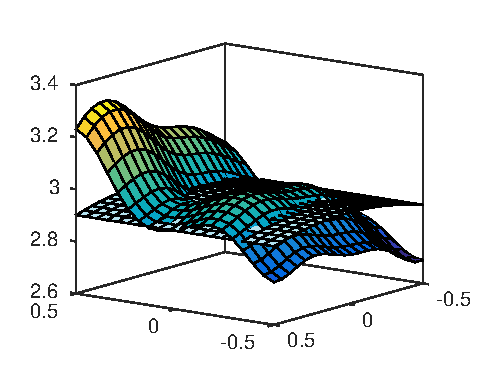
\includegraphics{plots/experiments/2dof/g11_hat.eps}
		%\caption{$\hat{W}_\varphi(t)$}
	\end{subfigure}
	\begin{subfigure}{0.5\textwidth}
		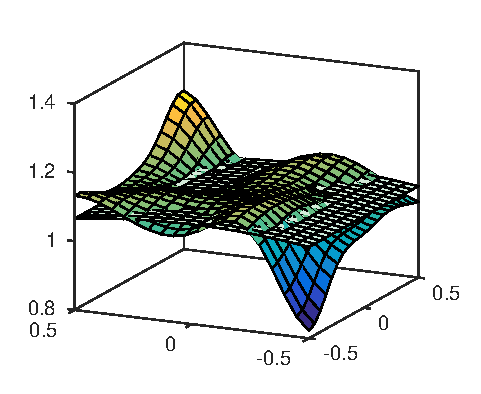
\includegraphics{plots/experiments/2dof/g12_hat.eps}
		%\caption{$\hat{W}_\gamma(t)$)}
	\end{subfigure}
	\caption{Σύγκριση των συναρτήσεων $\gamma_{11}(x)$ (αριστερά) και $\gamma_{12}(x)$ (δεξιά) με τις προσεγγίσεις τους $\hat{\gamma}_{11}(x)$ και $\hat{\gamma}_{12}(x)$ αντίστοιχα. Με γκρι (transparent) απεικονίζονται οι πραγματικές συναρτήσεις ενώ οι χρωματισμένες επιφάνειες είναι οι προσεγγίσεις αυτών. }
	\label{fig:2dof_g1_approximations}
\end{figure}

\begin{figure}
	\begin{subfigure}{0.5\textwidth}
		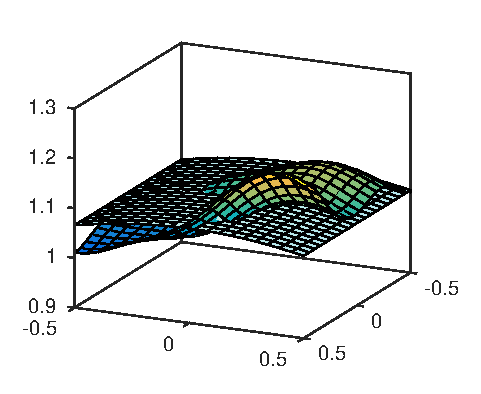
\includegraphics{plots/experiments/2dof/g21_hat.eps}
		%\caption{$\hat{W}_\varphi(t)$}
	\end{subfigure}
	\begin{subfigure}{0.5\textwidth}
		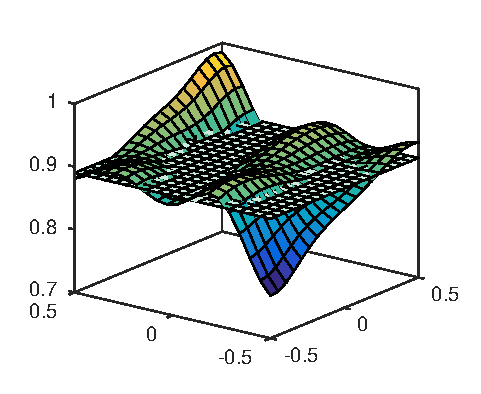
\includegraphics{plots/experiments/2dof/g22_hat.eps}
		%\caption{$\hat{W}_\gamma(t)$)}
	\end{subfigure}
	\caption{Σύγκριση των συναρτήσεων $\gamma_{21}(x)$ (αριστερά) και $\gamma_{22}(x)$ (δεξιά) με τις προσεγγίσεις τους $\hat{\gamma}_{21}(x)$ και $\hat{\gamma}_{22}(x)$ αντίστοιχα. Με γκρι (transparent) απεικονίζονται οι πραγματικές συναρτήσεις ενώ οι χρωματισμένες επιφάνειες είναι οι προσεγγίσεις αυτών. }
	\label{fig:2dof_g2_approximations}
\end{figure}


\section{Παρατηρήσεις}
\label{eq:remarks_on_exp}
Τέλος, σε αυτή την ενότητα παρουσιάζονται κάποιες παρατηρήσεις με βάση τα πειράματα που παρουσιάστηκαν στις Ενότητες \ref{sec:rbf_experiments} και \ref{sec:real_system_experiments}.\\

\begin{remark}
	Ο ρυθμός και η τελική ζώνη σύγκλισης των παραμετρικών σφαλμάτων $\tilde{W}(t)$ είναι άγνωστος και εξαρτάται από τις τιμές τόσο των κερδών $\beta_i$ όσο και από τα άγνωστα επίπεδα διέγερσης $a_1$ και $a_2$. Η βελτιστοποίηση αυτών των χαρακτηριστικών της διαδικασίας εκμάθησης μέσω ρύθμισης των παραμέτρων του σχήματος αναγνώρισης είναι μια δύσκολη διαδικασία καθώς δεν είναι ξεκάθαρο με ποιόν τρόπο επιδρά η κάθε παράμετρος στα άγνωστα επίπεδα διέγερσης.
	
	Για παράδειγμα, στο Πείραμα \ref{exampleB} φαίνεται πως τα βάρη δεν συγκλίνουν στις ακριβές τιμές τους αλλά σε μια περιοχή αυτών, και ως αποτέλεσμα οι προσεγγίσεις των συναρτήσεων $\gamma_{ij}(x)$ καταφέρνουν να προσεγγίσουν τις άγνωστες συναρτήσεις μόνο κατά μέση τιμή. Καθώς το πλάτος της περιοχής σύγκλισης εξαρτάται από τα άγνωστα επίπεδα διέγερσης, είναι δύσκολη η εύρεση παραμέτρων που θα επιφέρουν καλύτερα αποτελέσματα.\\
\end{remark}

\begin{remark}
	Το σχήμα αναγνώρισης είναι αρκετά απαιτητικό από υπολογιστικής άποψης. Το γεγονός αυτό, γίνεται εμφανές εάν θεωρήσει κανείς την διαδικασία αναγνώρισης ενός συστήματος ΠΕΠΕ.
	
	Για παράδειγμα, στο Πείραμα \ref{exampleB} προσεγγίζουμε τις άγνωστες συναρτήσεις με RBF δίκτυα τα οποία έχουν κέντρα σε ένα πλέγμα, όπου σε κάθε διάσταση τοποθετούνται 5 κέντρα. Ως αποτέλεσμα, για την αναγνώριση κάθε συνάρτησης $\varphi(x)$ χρειαζόμαστε $5^4$ βάρη, τα οποία υπολογίζονται κατά την διάρκεια του πειράματος μέσω αριθμητικής επίλυσης των διαφορικών εξισώσεων που ορίζουν οι νόμοι προσαρμογής. Μόνο για το διάνυσμα $\Phi$, απαιτείται η επίλυση $1250$ τέτοιων διαφορικών εξισώσεων. Επιπλέον, το μέγεθος της περιόδου είναι αρκετά μεγάλο, καθώς σε κάθε περίοδο πρέπει να επισκεφθούμε κάθε ένα από αυτά τα 650 κέντρα.
	
	Αν ωστόσο προσπαθούσαμε να προσεγγίσουμε με την ίδια στρατηγική έναν βραχίονα τριών βαθμών ελευθερίας το οποίο είναι ένα σύστημα έξι καταστάσεων, τότε μόνο για την αναγνώριση του διανύσματος $\Phi(x)$ θα απαιτούταν $3 \cdot 5^6 = 46875$ βάρη. Επίσης η περίοδος θα μεγάλωνε σε διάρκεια $25$ φορές, αφού πλέον θα πρέπει να επισκεφθούμε ακόμα περισσότερα κέντρα.
	
	Όπως είναι προφανές από τον παραπάνω συνειρμό, η εφαρμογή του σχήματος ελέγχου σε συστήματα μεγάλων διαστάσεων απαιτεί τεράστιους υπολογιστικούς πόρους.\\
\end{remark}

\begin{remark}
	\label{remakr:border_eval}
	Ενώ το σχήμα αναγνώρισης συνήθως παράγει αρκετά καλές εκτιμήσεις στο εσωτερικό του $\Omega_x$, οι προσεγγίσεις των συναρτήσεων φαίνεται να χάνουν ακρίβεια στο σύνορο του $\Omega_x$. Το φαινόμενο αυτό παρατηρείται τόσο στο Πείραμα \ref{exp:vdp} (ταλαντωτής \textit{Van Der Pol}) όσο και στο Πείραμα \ref{exampleB} (ρομποτικός βραχίονας). Σχετικά με αυτό το πρόβλημα παρουσιάζεται μια λύση στο Κεφάλαιο \ref{chap:conclusions}. \\
\end{remark}

\begin{remark}
	Από το Πείραμα \ref{exp:vdp} φαίνεται πως το σχήμα αναγνώρισης είναι ικανό να αναγνωρίσει συστήματα που δεν εμπίπτουν στην κατηγορία \textit{Euler Lagrange}. Ωστόσο, καθώς το πείραμα αυτό αποτελεί μεμονωμένο παράδειγμα, δεν μπορούμε να προχωρήσουμε στο συμπέρασμα ότι το σχήμα είναι ικανό να αναγνωρίσει κάθε τέτοιο σύστημα, συνεπώς απαιτείται επιπλέον έρευνα για την συγκεκριμένη υπόθεση.
\end{remark}
\chapter{Συμπεράσματα και Βελτιώσεις}
\label{chap:conclusions}
Σε αυτό το τελευταίο κεφάλαιο παρουσιάζουμε κάποια συμπεράσματα και παρατηρήσεις πάνω στα αποτελέσματα του Κεφαλαίου \ref{chap:experiments}. Το Κεφάλαιο αυτό αποτελείται από ένα πείραμα στο οποίο βγαίνουν κάποια συμπεράσματα σχετικά με την Συνθήκη Επιμένουσας Διέγερσης στην μεθοδολογία που αναπτύχθηκε στο Κεφάλαιο \ref{chap:scheme_presentation}, καθώς και από μια μέθοδο αξιολόγησης για πραγματικά συστήματα.



\section{Βελτιώσεις στο Σχήμα}
Σε αυτή την ενότητα, σκοπός είναι η μελέτη ενός συστήματος παρόμοιας δομής με αυτή του πειράματος αναγνώρισης του ρομποτικού βραχίονα που παρουσιάζεται στην Ενότητα \ref{exampleB}. Όπως είδαμε, στο σύστημα αυτό παρουσιάζεται το πρόβλημα ότι οι διακυμάνσεις των συναρτήσεων $\gamma_{ij}(x)$ είναι πολύ μικρές, με αποτέλεσμα η εκτίμηση να αποτελεί στην ουσία προσέγγιση της μέσης τιμής, αποτυγχάνοντας να εκτιμήσει τις μεταβολές των $\gamma_{ij}(x)$.

Αρχικά παρουσιάζουμε ένα σύστημα με συναρτήσεις παρόμοιας δομής με αυτές του συστήματος \ref{exampleB}. Το σύστημα αυτό περιγράφεται από τις εξισώσεις:
\begin{equation}
\label{eq:robotic_equiv_plant_form}
\begin{split}
\dot{x}_1 &= x_{2}  \\
\dot{x}_2 &= \gamma^{-1}(x)\varphi(x)+\gamma^{-1}(x)u(t)
\end{split}
\end{equation}
όπου
\begin{equation*}
\begin{split}
\varphi(x) &= \frac{\sin(x_1 + x_2)}{2} + 2.1 \sin(x_1) \\ 
\gamma(x) &= 0.03 \cos(x_1) + 0.075
\end{split}
\end{equation*}

Ζητούμενο μας είναι η αναγνώριση των άγνωστων συναρτήσεων $\varphi(x)$ και $\gamma(x)$, στο σύνολο $\Omega = [-\frac{\pi}{2},\frac{\pi}{2}]^2$. Το πρόβλημα εδώ είναι ότι η συνάρτηση $\gamma(x)$ έχει πολύ μικρό εύρος τιμών,και είναι μια τάξη μικρότερη από την συνάρτηση $\varphi(x)$, συνεπώς και εδώ περιμένουμε να εμφανιστεί ένα παρόμοιο πρόβλημα με αυτό της Υποενότητας \ref{exampleB}.

{  %% Wraptable Barrier
	\begin{wraptable}{r}{0.3\textwidth}
		\centering
		\captionsetup{format=plain}
		\caption{ Παράμετροι σχήματος αναγνώρισης}
		\label{tab:robot_equiv_schema_params}
		\begin{tabular}{ l | r }
			\hline\hline
			\text{Parameter} & Value \\ \hline\hline
			$k$             & $30$   \\ \hline
			$\lambda$       & $1 $   \\ \hline
			$\gamma_{f} \;\text{(bias)}$        & $0.05$ \\ \hline
			$\gamma_{f} \;\text{(gaussian)}$    & $6$ \\ \hline
			$\gamma_{g} \;\text{(bias)}$        & $0.05$  \\ \hline
			$\gamma_{g} \;\text{(gaussian)}$    & $0.06$ \\ \hline
			$\rho_0      $ & $4$  \\ \hline
			$\rho_\infty $ & $0.02$  \\ \hline
			$l           $ & $2$  \\ \hline
%			\text{επικάλυψη} & $75\%$  \\ \hline
%			$\sigma     \;\text{διασπορά} $ & $0.3550$   \\ \hline
			$\textit{ΔΤ}$   & $2$ 	\\ \hline \hline	
		\end{tabular}
	\end{wraptable}


	\subsection{Αρχική Προσέγγιση}
	\label{subsec:robot_like_init_approach}
	Για τον σκοπό αυτό ακολουθούμε την κλασσική μεθοδολογία της 
	Ενότητας \ref{subsec:CL_design}. Αρχικά, σχηματίζουμε τις προσεγγίσεις:
	\begin{equation*}
	\begin{matrix}
	\hat{\varphi}(x,t)  = \hat{W}_{\varphi}^T(t) Z_\varphi(x) & \text{και} & \hat{\gamma}(x,t) = \hat{W}_{\gamma}^T(t) Z_\gamma(x) 
	\end{matrix}
	\end{equation*}
	Τα κέντρα $c_\Phi$ των γκαουσιανών του διανύσματος οπισθοδρομητών $Z_\Phi$ ανήκουν στο σύνολο
	\begin{equation*}
	\mathcal{C}_\Phi = \bigtimes\limits_{i=1}^{2}  \begin{Bmatrix}
	-\frac{\pi}{2} + \frac{\pi}{5} k, \quad  k = 0,1,\dots,5
	\end{Bmatrix}
	\end{equation*}
	ενώ τα κέντρα $c_\gamma$ των οπισθοδρομητών $Z_\gamma$ ανήκουν στο σύνολο
	\begin{equation*}
	\mathcal{C}_\Gamma = \begin{Bmatrix}
	-\frac{\pi}{2} + \frac{\pi}{5} k, \quad  k = 0,1,\dots,5
	\end{Bmatrix}
	\end{equation*}
	σχηματίζοντας έτσι ένα πλέγμα που καλύπτει ομοιόμορφα τον χώρο $\Omega_x$. Οι υπόλοιποι παράμετροι του σχήματος αναγνώρισης δίνονται στον Πίνακα \ref{tab:robot_equiv_schema_params}.
	
}

\begin{figure}
	\begin{subfigure}{0.5\textwidth}
		% This file was created by matlab2tikz.
%
\definecolor{mycolor1}{rgb}{0.00000,0.44700,0.74100}%
\definecolor{mycolor2}{rgb}{0.85000,0.32500,0.09800}%
\definecolor{mycolor3}{rgb}{0.92900,0.69400,0.12500}%
\definecolor{mycolor4}{rgb}{0.49400,0.18400,0.55600}%
\definecolor{mycolor5}{rgb}{0.46600,0.67400,0.18800}%
%
\begin{tikzpicture}

\begin{axis}[%
width=0.761\textwidth,
height=0.65\textwidth,
at={(0\textwidth,0\textwidth)},
scale only axis,
xmin=0,
xmax=150000,
xlabel style={font=\color{white!15!black}},
xlabel={Time, $t$},
ymin=-1,
ymax=0.6,
ylabel style={font=\color{white!15!black}},
ylabel={$\hat{W}_\varphi(t)$},
axis background/.style={fill=white},
xmajorgrids,
ymajorgrids
]
\addplot [color=mycolor1, line width=1.2pt, forget plot]
  table[row sep=crcr]{%
0	0\\
112	-0.00873191104619764\\
252.002922924992	-0.00229466499877162\\
390.217907305429	-0.000455850618891418\\
932	0.00318693710141815\\
1496.00172303006	0.00392978545278311\\
2888.0038229152	0.00915909631294198\\
3025.64645681018	0.0103304294170812\\
3160.63642549998	0.0104591465205885\\
3297.95829501448	0.00992129484075122\\
3704.22632865372	0.0115461019740906\\
4384.35533080128	0.0141832788358442\\
4522.36106055698	0.0136845212546177\\
5067.44815347614	0.0156446928449441\\
5340.00035741119	0.016142228996614\\
5612	0.0178925347572658\\
5747.78535528871	0.0172366981278174\\
6830.74333044892	0.0212177752400748\\
6964.59542264536	0.0207800611678977\\
7232.18183707527	0.0218627524736803\\
7498.04240214167	0.0225146826123819\\
7630	0.0236132294521667\\
7760.16397159177	0.0229890027840156\\
8162.72801693904	0.0244390543084592\\
8434.1868868389	0.0251319800154306\\
8567.74742263558	0.0261763836897444\\
8703.09539325375	0.0263617231976241\\
8840.11237491711	0.0259281377948355\\
9653.32876287354	0.0285907603683881\\
9790.01421757895	0.0294138033350464\\
10060.0181288694	0.0290790778817609\\
10468.0896803576	0.030355884169694\\
10737.3268692077	0.0310045023506973\\
10873.3782956566	0.0322736002854072\\
11280.001628508	0.0323836871248204\\
11817.7124345982	0.0334050914971158\\
11952.0104406828	0.0345328209514264\\
12084.3291409557	0.0338256533141248\\
12478.0159813345	0.0349768662417773\\
12614.0055732056	0.0349542565236334\\
12884.1759072875	0.0365301193960477\\
13019.40599186	0.0358505865442567\\
13422.0807327526	0.0369585248117801\\
13828.8045997246	0.0380495059944224\\
13966.3601993713	0.0388369198190048\\
14648.4510980735	0.03970961808227\\
15328.8523046888	0.0415759121242445\\
15464.7694424407	0.041163205052726\\
15736.7810497772	0.0419708905683365\\
16282.1685552629	0.042951115698088\\
16554.8072660132	0.0441245558904484\\
16691.095167162	0.0435327581944875\\
17774.208211859	0.0463801782461815\\
17911.3470301021	0.0459687374823261\\
18320.2008020447	0.0469948822574224\\
18724.5713473966	0.0480348051351029\\
18858.7596925187	0.0485633232165128\\
18994	0.0480570443614852\\
19263.4832541025	0.0487194990564603\\
19668.0119813944	0.0492706479562912\\
19802.0030973446	0.0503390062076505\\
19937.6616359446	0.0506458863092121\\
20073.4977807108	0.0501533502247185\\
20343.8890875441	0.050894232786959\\
20883.9425577292	0.052183798776241\\
21018.2855922223	0.0526910102635156\\
21154.2748149521	0.0522116220672615\\
21555.8884175563	0.0531852292187978\\
21821.634642505	0.0537654768850189\\
21958.0020177541	0.0545704261166975\\
22089.3883683379	0.0539867569168564\\
22747.3701267941	0.0559165704180487\\
22880.2518612494	0.0553742203337606\\
23138.0043554613	0.0561302844726015\\
23268.1926153055	0.0559397385513876\\
23399.7397710408	0.057092404254945\\
23530.0021849063	0.0565219744748902\\
24310.3786538444	0.0579294830095023\\
24566.7161762832	0.0582795793015976\\
24694.005302219	0.0591962600301486\\
24822.0073580407	0.058618579962058\\
25451.2188825755	0.0597558563749772\\
25942.621367503	0.060468211537227\\
26068.1504304868	0.0610213005275\\
26194.6796458697	0.060683093033731\\
26710.0017447101	0.0622357692627702\\
26840.7909855786	0.06162268971093\\
27493.401553682	0.0628671613230836\\
28013.7975394751	0.0636032350594178\\
28147.9341682471	0.0642325458175037\\
28278.1196751107	0.0637315455824137\\
29206.0244418008	0.0651748824457172\\
29604.1415260042	0.0655116504640318\\
29738.0031800529	0.0664540514990222\\
31326	0.0683653904707171\\
31459.0831710222	0.0689330924069509\\
31592.7402741527	0.0685048003215343\\
32392.3752419029	0.0701724389218725\\
32527.2733923536	0.0698302890523337\\
33469.8710001491	0.071614687301917\\
33606.09671395	0.0712795493309386\\
34412.5564448251	0.0729647582338657\\
34545.0509871586	0.0724657048122026\\
35346.5803560152	0.0740224585460965\\
35484.0238190253	0.0735062968742568\\
40346.4398112328	0.0794570511498023\\
40614.6774691055	0.079805846355157\\
40886.0032711443	0.0803874028206337\\
41022	0.0799707706319168\\
41425.1174932484	0.0806319420516957\\
41557.1949180839	0.0804562473203987\\
41690.1432134393	0.0812140999769326\\
42764.5083397912	0.0824124464706983\\
42898.0032832935	0.0819248284387868\\
43440.3053669854	0.0826275257568341\\
44645.2741505332	0.083799269516021\\
44780.0049651841	0.0843451050168369\\
44915.7275081078	0.0838727536029182\\
50964.9683064648	0.0897713299200404\\
51776.2659334236	0.0905731927487068\\
51910.4433192842	0.0911987067083828\\
52044.0053765394	0.0906803516263608\\
52856.0010282169	0.0914215347729623\\
52991.4013770175	0.0920859612815548\\
53939.9837553777	0.0921465138962958\\
54206.000683456	0.0929695689992514\\
54339.5719722534	0.0925865480676293\\
55150.1290798635	0.0939593476359732\\
55417.5116007938	0.093658381694695\\
56767.2089047726	0.0947841356683057\\
57170.349474323	0.095377176447073\\
57978.3021123107	0.0955268321849871\\
58114.0065143806	0.0955295395397115\\
58247.7281872005	0.0963202458224259\\
58380.5207084554	0.0957934779580683\\
59862.7261869357	0.0969147460127715\\
60130.0581894843	0.0968350744224153\\
60265.5328945834	0.0977092843386345\\
61210.5167350034	0.0975874640571419\\
61344.0417749969	0.0983401848934591\\
62288.8272827867	0.0984915630833711\\
62424	0.0990850999951363\\
63238.4204461284	0.0990344202436972\\
73184.5743180882	0.10458996554371\\
73453.3167447994	0.104483993491158\\
73584.1919374071	0.105230442452012\\
74526.0097902838	0.105248560197651\\
74662.2730076718	0.105693685472943\\
74931.7043770058	0.105198158504209\\
75738.00518815	0.106071542162681\\
76007.4484841932	0.105741894542007\\
77495.0645770783	0.106363400263945\\
77766.0096714511	0.106690762506332\\
77901.6846145824	0.107116790895816\\
78169.9489901577	0.106743287848076\\
79248.0014063443	0.107339034846518\\
81944.2338433389	0.10835333072464\\
82080.001339636	0.108927323395619\\
82886.590667449	0.108656318567228\\
83154.4874666953	0.109262196638156\\
83422.1057192109	0.108938224206213\\
84900.0007993603	0.109383416798664\\
85033.022115836	0.110125450446503\\
85972.0489529709	0.110250865458511\\
86108.0057996012	0.110472051688703\\
86377.8697648019	0.11008697169018\\
86785.3334195038	0.110314911202295\\
87052.0065432613	0.110591124830535\\
87186.4127551906	0.110812978236936\\
87456.6409229668	0.110537664993899\\
89067.2632409489	0.111251258407719\\
89202.0237729485	0.11152913729893\\
89470.0140514718	0.11118765512947\\
92435.2734661067	0.112173098052153\\
93245.1200776116	0.112562181981048\\
93380.6079752721	0.112965954875108\\
93651.3869358163	0.112531401595334\\
94594.0270253877	0.112858985638013\\
96342.0641796422	0.113508267299039\\
96478.0251018841	0.113866971689276\\
96748.0012214776	0.113406337593915\\
97694.0437853558	0.114098916266812\\
97962.8668488259	0.113875893148361\\
100928.069362075	0.114605483686319\\
101596.536200154	0.115084201301215\\
101730.703158302	0.115297751908656\\
102000.001202245	0.11497006972786\\
105763.916846722	0.116245915123727\\
106038.000939227	0.115836684446549\\
109535.662525501	0.116635655227583\\
109666.889280565	0.116594386548968\\
109799.943372881	0.117163637129124\\
110068.0077277	0.116635275364388\\
110470.741871986	0.116680419421755\\
110604.020952383	0.116683879401535\\
110737.274427209	0.117524301633239\\
111138.319163931	0.116961472202092\\
113004	0.11731671099551\\
113408.358081424	0.117374562192708\\
113543.76571871	0.117897584947059\\
113811.848079944	0.117369222891284\\
114620.489244147	0.118076227721758\\
114889.922178919	0.117667594371596\\
115956.008476907	0.117978612368461\\
118091.008918741	0.118185158935376\\
118223.505863055	0.118788502877578\\
118489.934573053	0.118351290613646\\
119153.02046296	0.1188758535136\\
119422.066014303	0.118560418108245\\
120360.264199572	0.11874417681247\\
126900.332750372	0.120059192558983\\
127303.523397554	0.120019893278368\\
127436.181559941	0.120506095117889\\
127700.017249848	0.120161437604111\\
128766.006568941	0.120371100521879\\
129032.083173219	0.120330576581182\\
129163.586852788	0.120778996235458\\
129430.093747879	0.120435225166148\\
130638.013198067	0.120649482356384\\
130907.968299526	0.120527210674481\\
131040.110241626	0.12116651359247\\
131839.867808036	0.120721289888024\\
131971.715218584	0.121174727770267\\
132237.424850015	0.120812835521065\\
133301.911427985	0.120925968862139\\
134091.892996055	0.121016609977232\\
135020.050011789	0.121054662507959\\
135154.015307092	0.120937687548576\\
135287.560127047	0.121613684372278\\
135552.002629405	0.121177952445578\\
136868.006861544	0.121744682692224\\
137132.87039335	0.121303826483199\\
137802.025085811	0.121872175717726\\
138067.400339053	0.121492817212129\\
138985.796227699	0.12159761111252\\
139116.000830304	0.121460722642951\\
139247.591079049	0.12206780037377\\
139508.255055602	0.121680959884543\\
140174.775468485	0.12212960596662\\
140443.216233102	0.121793486439856\\
141902.000580666	0.122272813023301\\
142167.518093407	0.122020895971218\\
142566.079602554	0.122156844474375\\
142700.680740228	0.122488338849507\\
142970.386099051	0.122060738125583\\
143902.844413685	0.12227488210192\\
};
\addplot [color=mycolor2, line width=1.2pt, forget plot]
  table[row sep=crcr]{%
0	0\\
112	-0.901030665496364\\
252.002922924992	-0.820398941374151\\
390.217907305429	-0.73581109996303\\
530.005529629852	-0.690094701421913\\
798	-0.664794999669539\\
932	-0.653792190249078\\
1069.63117093686	-0.647444478556281\\
1211.18022928806	-0.644261231442215\\
1354.12820086977	-0.642943162645679\\
1496.00172303006	-0.642931391252205\\
1916.0019269498	-0.64828371303156\\
2196.01523052368	-0.654479655233445\\
2334.46960754279	-0.654440668819007\\
2472.22403558512	-0.657213373604463\\
2612.28981323258	-0.663934190117288\\
2749.83822614883	-0.666980833397247\\
2888.0038229152	-0.668318573036231\\
3160.63642549998	-0.672959022020223\\
3432.70378484437	-0.680322015512502\\
3566.64990431615	-0.683055573346792\\
3704.22632865372	-0.680625664361287\\
3840.0412063291	-0.680857887433376\\
3976.06519036714	-0.68813779586344\\
4114.07935921708	-0.694349755212897\\
4248.95258628519	-0.69495241731056\\
4384.35533080128	-0.696314456494292\\
4792.00479713475	-0.703538426198065\\
4930.54604780124	-0.702706078416668\\
5203.52043875042	-0.704528448666679\\
5340.00035741119	-0.712435238383478\\
5475.0359938975	-0.711748202651506\\
5612	-0.713051987870131\\
5747.78535528871	-0.715821416699328\\
5881.95759932778	-0.717050288571045\\
6016.55274945017	-0.716563713882351\\
6154.01310307815	-0.715283638128312\\
6289.10173325468	-0.713317771151196\\
6424.00839691641	-0.722806134290295\\
6559.91597963241	-0.72438994483673\\
6696.00301343808	-0.724507187958807\\
6830.74333044892	-0.726805059908656\\
7098.00979751931	-0.728788324340712\\
7232.18183707527	-0.72510292113293\\
7366.86271562381	-0.730253811751027\\
7498.04240214167	-0.73337932585855\\
7630	-0.73189087814535\\
7760.16397159177	-0.732750575552927\\
7892.73702282901	-0.735053384298226\\
8027.07541730977	-0.733089496381581\\
8162.72801693904	-0.731722080585314\\
8300.15128390043	-0.733057941717561\\
8434.1868868389	-0.740483123896411\\
8567.74742263558	-0.739350169256795\\
8703.09539325375	-0.739800850249594\\
8840.11237491711	-0.741192824556492\\
9112.70621861215	-0.742966343415901\\
9248.6055115159	-0.737758003320778\\
9384.03656778787	-0.736151405668352\\
9519.34683969503	-0.74356954486575\\
9653.32876287354	-0.748814511054661\\
9790.01421757895	-0.748239730746718\\
10332.654433774	-0.75059257587418\\
10468.0896803576	-0.744466343981912\\
10602.0091945135	-0.747465342108626\\
10737.3268692077	-0.753618788323365\\
10873.3782956566	-0.752583405002952\\
11280.001628508	-0.754237739631208\\
11413.3033445601	-0.753809874062426\\
11546.1695853747	-0.745364654314471\\
11682	-0.753418144711759\\
11817.7124345982	-0.758523728058208\\
11952.0104406828	-0.757146696967538\\
12214.7450288067	-0.757195544720162\\
12344.0339181967	-0.751580017997185\\
12478.0159813345	-0.750335168093443\\
12614.0055732056	-0.761283328291029\\
12748.3552542587	-0.759594985400327\\
12884.1759072875	-0.75853503466351\\
13019.40599186	-0.759413736261195\\
13153.3500999383	-0.758171571040293\\
13288	-0.758658790204208\\
13422.0807327526	-0.753942391864257\\
13558.0011445609	-0.751712928875349\\
13693.8750315855	-0.759078326373128\\
13966.3601993713	-0.760999107413227\\
14102.5317061869	-0.759329435473774\\
14238	-0.762339380511548\\
14374	-0.762787971645594\\
14510.3301060171	-0.764458810037468\\
14648.4510980735	-0.759750008495757\\
14784.2263407932	-0.755880844051717\\
14919.3735909734	-0.76304332644213\\
15057.0946069513	-0.766522549383808\\
15193.662576115	-0.766921764123254\\
15328.8523046888	-0.765560073399683\\
15464.7694424407	-0.76852083709673\\
15600.104814617	-0.767879991995869\\
15736.7810497772	-0.770117572479649\\
15874.8769210593	-0.766303769487422\\
16011.5137242898	-0.764225625607651\\
16146.1326965609	-0.768707574956352\\
16282.1685552629	-0.77397768071387\\
16418.5415995807	-0.773010762466583\\
16554.8072660132	-0.774306448263815\\
16691.095167162	-0.771866148163099\\
16964.3589344957	-0.771322110609617\\
17101.1902308014	-0.772641777788522\\
17234.5923098653	-0.766599754395429\\
17369.6476332788	-0.769253544451203\\
17502.0519832455	-0.773700217891019\\
17774.208211859	-0.776754586055176\\
17911.3470301021	-0.774749393574893\\
18184.0277862177	-0.774576129508205\\
18320.2008020447	-0.767753185995389\\
18453.3578733352	-0.770993050449761\\
18588.0068359114	-0.779303476971108\\
18724.5713473966	-0.776365539582912\\
18858.7596925187	-0.778863885032479\\
18994	-0.780659471667605\\
19263.4832541025	-0.78095545436372\\
19397.7252908056	-0.777699924830813\\
19532.0397443481	-0.776436997868586\\
19668.0119813944	-0.783655645878753\\
19802.0030973446	-0.781546106591122\\
19937.6616359446	-0.780948561208788\\
20073.4977807108	-0.782580491912086\\
20208.4377923581	-0.784980623197043\\
20343.8890875441	-0.783977847924689\\
20482.0088856405	-0.780589328234782\\
20617.2496686857	-0.774617678485811\\
20750	-0.786585351626854\\
20883.9425577292	-0.784432315675076\\
21018.2855922223	-0.785844118363457\\
21154.2748149521	-0.785479988902807\\
21287.2414559791	-0.782406804530183\\
21422.1586694331	-0.781771262612892\\
21555.8884175563	-0.776982060808223\\
21690.068587861	-0.779392966476735\\
21821.634642505	-0.78441014373675\\
21958.0020177541	-0.783593759959331\\
22220	-0.785846864921041\\
22352.3366759736	-0.778268265974475\\
22483.6622971285	-0.777221656462643\\
22616.0149522627	-0.78633124078624\\
22747.3701267941	-0.785764924716204\\
22880.2518612494	-0.787446065543918\\
23009.8165615977	-0.78767749920371\\
23138.0043554613	-0.777865670097526\\
23268.1926153055	-0.788522759918123\\
23530.0021849063	-0.787529193621594\\
23660.7227060786	-0.788730524422135\\
23792.3020496496	-0.783573269785848\\
23921.2764467227	-0.782437024696264\\
24051.3391778861	-0.78935786098009\\
24310.3786538444	-0.791257539152866\\
24438.6083746319	-0.785204404935939\\
24566.7161762832	-0.786792917730054\\
24694.005302219	-0.793042689590948\\
24822.0073580407	-0.792185100901406\\
24950.002527282	-0.793762356537627\\
25076.3213704281	-0.787405306356959\\
25199.5533322484	-0.792121689533815\\
25322.6265292946	-0.792958918289514\\
25451.2188825755	-0.789917254151078\\
25570.3769820849	-0.79440418141894\\
25692.2230035416	-0.792935329314787\\
25817.1319369696	-0.793038499192335\\
25942.621367503	-0.788850731769344\\
26068.1504304868	-0.792721090721898\\
26194.6796458697	-0.791642227210104\\
26322	-0.79399848828325\\
26451.1931058393	-0.788347235444235\\
26578.2373760629	-0.794447319756728\\
26710.0017447101	-0.79143078517518\\
26840.7909855786	-0.794197413139045\\
26972.0148683393	-0.79464708614978\\
27104.0025234307	-0.78921780505334\\
27233.1061668737	-0.788773828215199\\
27362.6591868793	-0.796238130627898\\
27493.401553682	-0.794208682404133\\
27624.0064250366	-0.795012518763542\\
27756.3327519629	-0.794226371013792\\
27885.6409076466	-0.788439543393906\\
28013.7975394751	-0.79644437727984\\
28412.9807002435	-0.796186396008125\\
28547.8208160142	-0.797828539274633\\
28678.1429405105	-0.791339745337609\\
28810.0101784541	-0.796409684699029\\
28942	-0.79683261847822\\
29074	-0.797928851970937\\
29339.5575938213	-0.798527455423027\\
29473.57217346	-0.788574419391807\\
29604.1415260042	-0.797021386621054\\
29738.0031800529	-0.798704502638429\\
30002.7025076879	-0.80033860495314\\
30136.4036968845	-0.801685356273083\\
30267.634374416	-0.79682639890234\\
30398.5488258564	-0.795715778105659\\
30530.5903711248	-0.802549119543983\\
30661.3477255369	-0.803242303576553\\
30927.5631486405	-0.80313931076671\\
31059.8090897388	-0.798642782407114\\
31192.2793728838	-0.803609431022778\\
31326	-0.803700729535194\\
31459.0831710222	-0.805296046746662\\
31592.7402741527	-0.805750666855602\\
31726.003409319	-0.807172885834007\\
31859.7214506428	-0.807756819645874\\
31992.8691410239	-0.797963790013455\\
32125.9493569711	-0.806028887367574\\
32258.6435181734	-0.808565714774886\\
32392.3752419029	-0.807476861955365\\
32527.2733923536	-0.808873906556983\\
32660.0956164064	-0.807125776744215\\
32794.2538717002	-0.801985852711368\\
32928.5688926536	-0.797810174379265\\
33064.7921765206	-0.801161468785722\\
33198.0074246936	-0.80604226180003\\
33334	-0.808127229305683\\
33741.3656299961	-0.808787083427887\\
33877.488053372	-0.80942353757564\\
34010.0188942721	-0.801460949296597\\
34144.0338897276	-0.808284678612836\\
34280.001281485	-0.810036094830139\\
34678.8083625658	-0.811683070496656\\
34812.0178180393	-0.811000914109172\\
34945.8286497429	-0.803138839517487\\
35078.0002648872	-0.811401281593135\\
35210.8291793698	-0.811071245319908\\
35346.5803560152	-0.808306888473453\\
35484.0238190253	-0.810658719128696\\
35620	-0.811380394239677\\
35754.3339887734	-0.811029627686366\\
35890.4031632434	-0.806167166156229\\
36024.7443273624	-0.800537524046376\\
36159.3825077138	-0.804572599008679\\
36292.2599713471	-0.809279246197548\\
36832.0165189321	-0.810375147382729\\
36968.0137767881	-0.803558280837024\\
37236.1150781914	-0.811618421139428\\
37504.008755804	-0.811985994689167\\
37640.1471179233	-0.809652380063199\\
37910.0484066397	-0.812303457059897\\
38042.3722078732	-0.804497505741892\\
38177.2920230122	-0.805615487479372\\
38314.0030396795	-0.812839624675689\\
38450.0063556313	-0.811747572675813\\
38586.1169130985	-0.81303591968026\\
38721.2117588893	-0.812241704610642\\
38857.3569036643	-0.812845503620338\\
38993.7371582648	-0.811303971568123\\
39129.8227790919	-0.810521500010509\\
39264.0280171332	-0.805818936583819\\
39534.8941150735	-0.812748532101978\\
39808.0846360379	-0.813503749639494\\
39942.7152869941	-0.81400470357039\\
40212	-0.814054189308081\\
40346.4398112328	-0.808714457962196\\
40480.2548446514	-0.814507395407418\\
40614.6774691055	-0.814530933450442\\
40751.3896925234	-0.816026321874233\\
40886.0032711443	-0.814837755955523\\
41158.0015440524	-0.81546125409659\\
41292.1310790393	-0.814338153548306\\
41425.1174932484	-0.807296732527902\\
41557.1949180839	-0.814268471178366\\
41690.1432134393	-0.814886868407484\\
41824	-0.816203337541083\\
41957.2922195599	-0.815433701092843\\
42092.334948483	-0.81641777875484\\
42226.7912285435	-0.813787664461415\\
42359.033838611	-0.815399057319155\\
42494.6732044409	-0.812190723256208\\
42628.2910438594	-0.817040550347883\\
42764.5083397912	-0.818101802055025\\
43032.3048589773	-0.818106228049146\\
43166.0114920685	-0.817310564743821\\
43305.9747374147	-0.813242463918868\\
43440.3053669854	-0.810307979787467\\
43575.3792850583	-0.812633238529088\\
43707.6861342708	-0.817798383184709\\
43976.0421364434	-0.818623223109171\\
44111.0990260874	-0.814779169071699\\
44245.9839948486	-0.817189207446063\\
44380.2823320313	-0.812979737267597\\
44515.8367629609	-0.812548735120799\\
44645.2741505332	-0.818662434670841\\
44915.7275081078	-0.819637515640352\\
45184.3970553146	-0.819790284469491\\
45320.6546549018	-0.815278500813292\\
45452.1087246966	-0.812376654648688\\
45584.3719430878	-0.817617190215969\\
45719.5650739855	-0.820069491310278\\
45986.6851726146	-0.819979568244889\\
46122.0016511747	-0.818919039971661\\
46254.0090728773	-0.815984286222374\\
46386.0005108499	-0.818210561585147\\
46519.5225508256	-0.821727588889189\\
46790.2716873867	-0.818869681796059\\
46927.7949892317	-0.818457398825558\\
47060.3049622759	-0.818761883099796\\
47196.1207280638	-0.818018450780073\\
47330.0185026058	-0.810237445897656\\
47464.006600318	-0.815537023387151\\
47597.0042633725	-0.817759653436951\\
47866.5820241336	-0.818553929246264\\
48002.5169622099	-0.820085967687191\\
48274.4017008019	-0.815679661580361\\
48410.0093368144	-0.813204925623722\\
48547.1327454824	-0.815088182949694\\
48678.0371324653	-0.815401984553318\\
48814.3197368876	-0.819672316749347\\
48950.005669016	-0.820142258628039\\
49355.3522825034	-0.817716041812673\\
49487.1552794789	-0.819705085334135\\
49618.3015558335	-0.819403873407282\\
50292.3321327796	-0.821861760196043\\
50428.8193392032	-0.819550366781186\\
50564.1777726591	-0.818068726221099\\
50696.4905127079	-0.818734107277123\\
50830.8361384078	-0.820932749309577\\
50964.9683064648	-0.821350818121573\\
51102.5330463203	-0.822407926112646\\
51237.4495948614	-0.822492614184739\\
51373.1940387927	-0.821017157868482\\
51641.021206004	-0.816831305128289\\
51776.2659334236	-0.822154522640631\\
51910.4433192842	-0.823749188624788\\
52044.0053765394	-0.823107866075588\\
52451.5875307856	-0.824098665296333\\
52586.018820324	-0.819472816336202\\
52720.1474329586	-0.824220006994437\\
53394.2615928621	-0.825966173986671\\
53532	-0.8245752560033\\
53667.7958355415	-0.820109556196257\\
53805.4932371948	-0.819648542703362\\
54074.0180963461	-0.825376105000032\\
54339.5719722534	-0.824383716011653\\
54612	-0.824972919886932\\
54746.0038789641	-0.819571260886732\\
54881.2110038355	-0.817929175449535\\
55015.7235232282	-0.825171201024204\\
55150.1290798635	-0.824542283517076\\
55552.1529602451	-0.825762951222714\\
55825.2099759246	-0.820551134762354\\
55958.2930295095	-0.825028561870568\\
56092.0849112505	-0.824062066240003\\
56228.2970272021	-0.825828145112609\\
56364.9638171407	-0.825063850817969\\
56498.4054749402	-0.822505290154368\\
56632.0667863313	-0.823853202164173\\
56767.2089047726	-0.820878324273508\\
56900.0855554101	-0.820498561050044\\
57036.0005134662	-0.822906347602839\\
57303.6949357393	-0.824495912092971\\
57440.1488693497	-0.825018887146143\\
57575.3257611515	-0.823826933774399\\
57708.3716537187	-0.823629479127703\\
57843.1693741531	-0.818913571652956\\
57978.3021123107	-0.822296802740311\\
58114.0065143806	-0.824673967028502\\
58380.5207084554	-0.825344641372794\\
58513.251007276	-0.82314485264942\\
58646.9948168729	-0.82392936971155\\
58782.0280934203	-0.822604192682775\\
58916.3637825826	-0.821953909413423\\
59187.0643437761	-0.825831239752006\\
59726.5289620517	-0.826339858409483\\
59996.4250352861	-0.818245880043833\\
60130.0581894843	-0.824639399856096\\
60404.1649764004	-0.825450197589817\\
60539.4291162074	-0.82420262042433\\
60674.1741191354	-0.825688855431508\\
60810.5855699076	-0.825458351930138\\
60944.3880570454	-0.822055284195812\\
61076.215915892	-0.8216246587981\\
61344.0417749969	-0.826560031855479\\
61614	-0.826646402711049\\
61749.8958418175	-0.824938064120943\\
61884.1515736743	-0.825433706952026\\
62018.7506536032	-0.823411298566498\\
62152.018654846	-0.825066525983857\\
62288.8272827867	-0.823824023886118\\
62424	-0.825312234490411\\
62693.7990329725	-0.826720589800971\\
62830.3557464709	-0.826348757836968\\
62966.9911535815	-0.82705690342118\\
63104.4264342427	-0.822899807943031\\
63238.4204461284	-0.823300426622154\\
63513.9131685144	-0.827212977252202\\
63781.3359398315	-0.825825631705811\\
63916	-0.826964473817497\\
64050.1863205639	-0.827204062545206\\
64187.445028432	-0.826533703366295\\
64322	-0.823201831342885\\
64456	-0.825788102461956\\
64594.0003827496	-0.827354040724458\\
65127.2381843167	-0.826068532041973\\
65262.9074171533	-0.823475361074088\\
65399.5449190223	-0.823063611605903\\
65800	-0.827395775035257\\
65936.0091759489	-0.826633118296741\\
66204.3742012746	-0.827878409385448\\
66337.9425987218	-0.821583988436032\\
66472.0377427266	-0.825032673659734\\
66604.2243351558	-0.826188539969735\\
66738.0068528057	-0.828315672435565\\
66872.2866011599	-0.828499143972294\\
67004.7498360672	-0.829490867938148\\
67139.6334604781	-0.827631242398638\\
67273.5125035252	-0.824373914307216\\
67406.1511375386	-0.827807917637983\\
67542.00941945	-0.827967406454263\\
67678.5610396955	-0.829996821266832\\
68080.5577444216	-0.829704813775606\\
68217.2664463645	-0.827294458402321\\
68351.8095484515	-0.82598806428723\\
68485.0602303592	-0.823731801094254\\
68756.0025520448	-0.829071882151766\\
68888.1682555858	-0.830780213786056\\
69020.5416335553	-0.830362485954538\\
69156.0085282629	-0.829283207131084\\
69290.4441082565	-0.826117158896523\\
69426.5846574412	-0.826364838401787\\
69694.0004762716	-0.829514021635987\\
69828.1225875389	-0.829922252713004\\
69962	-0.827193836303195\\
70095.1562641033	-0.8309929970128\\
70232	-0.827746331255184\\
70366.0490155918	-0.826416473166319\\
70498.6332206115	-0.827135268657003\\
70632.0202395909	-0.829549083689926\\
70766	-0.83102600829443\\
71032.7003673608	-0.828664280386874\\
71168.5205490974	-0.825472309341421\\
71303.7781612994	-0.825069785991218\\
71436.8369501301	-0.827764021523762\\
71570.4516055383	-0.829222052299883\\
71704.9335051667	-0.829656670481199\\
71838.669396541	-0.830823636904825\\
72246.0050688251	-0.829057167400606\\
72378.3475625111	-0.830278345471015\\
72511.2859747774	-0.830055139493197\\
72647.6742265893	-0.830534025240922\\
72916.8559051328	-0.830093276133994\\
73048.5355816992	-0.830819328752114\\
73184.5743180882	-0.826251662860159\\
73318.7285979621	-0.830150940251769\\
73453.3167447994	-0.828195071866503\\
73584.1919374071	-0.830770330270752\\
73720.3594621349	-0.831739596265834\\
74128.0128925699	-0.83238319636439\\
74261.5878328651	-0.828058077662718\\
74394.0612394329	-0.830325410846854\\
74526.0097902838	-0.829609787440859\\
74662.2730076718	-0.832410717732273\\
75066.0049253786	-0.833188327174867\\
75201.9146497864	-0.829629577550804\\
75335.9778097816	-0.829048977437196\\
75470.1159973658	-0.830828536301851\\
75604.3915648087	-0.831616271287203\\
75738.00518815	-0.833320292964345\\
75872.197889179	-0.830962582433131\\
76142.7082352535	-0.833135582885006\\
76276.6623090605	-0.83189542524633\\
76412.0113435062	-0.829684825584991\\
76548.0004123329	-0.832174677780131\\
76682.6394464825	-0.833941073855385\\
76820.1827740584	-0.833925758779515\\
76952.6637482011	-0.835025124775711\\
77357.8691144849	-0.831426052347524\\
77495.0645770783	-0.833051710680593\\
77628.276721034	-0.831231203570496\\
77766.0096714511	-0.830393797077704\\
77901.6846145824	-0.832291463768343\\
78035.3177995619	-0.833266266534338\\
78169.9489901577	-0.832713032723404\\
78301.6648236099	-0.830979465303244\\
78436.5246737876	-0.831887581560295\\
78572.0173205022	-0.829636266280431\\
78706.3211631442	-0.833626621926669\\
79384.0045676998	-0.83430908631999\\
79520.4312861045	-0.831206676521106\\
79653.925256369	-0.83131639752537\\
79787.0258889775	-0.83263881545281\\
79921.8275530324	-0.834696789941518\\
80190	-0.835098291106988\\
80325.6825382432	-0.83410978858592\\
80459.1322491131	-0.830425538442796\\
80594.0879669618	-0.828325625334401\\
80728.5494615272	-0.830244383745594\\
80864.0028320173	-0.831206396513153\\
80999.0898471469	-0.831040347256931\\
81268.3980742903	-0.832798807037761\\
81402.2276324158	-0.833643715130165\\
81538.5170580754	-0.830079490900971\\
81673.9010101482	-0.829053114401177\\
81810.2030728246	-0.833087832841557\\
81944.2338433389	-0.83253912490909\\
82080.001339636	-0.834507492108969\\
82484.7529113025	-0.832435758493375\\
82618.2854592938	-0.826346209272742\\
82752.0016474929	-0.82799165166216\\
82886.590667449	-0.825662196177291\\
83020.0012092105	-0.830153111484833\\
83154.4874666953	-0.832333221391309\\
83558	-0.83275590869016\\
83690.0899033071	-0.830930879543303\\
83954.0234923227	-0.833288585825358\\
84088.0159625818	-0.832886779098772\\
84222.97584821	-0.833096529066097\\
84358	-0.832667227921775\\
84495.7343120249	-0.833917025680421\\
84632.181651763	-0.829548312030965\\
84766.0222488895	-0.829086758894846\\
84900.0007993603	-0.83072432372137\\
85033.022115836	-0.833105729165254\\
85169.1220651787	-0.833706538629485\\
85301.0230863734	-0.830876180989435\\
85435.586212333	-0.833840023813536\\
85572	-0.834632018086268\\
85706.0622424201	-0.829659148410428\\
85838.0621571056	-0.830642855347833\\
85972.0489529709	-0.830932455108268\\
86108.0057996012	-0.834079015592579\\
86377.8697648019	-0.834393173863646\\
86512.1802040523	-0.83547883835854\\
86650.0464830288	-0.832905646559084\\
86785.3334195038	-0.827508132468211\\
86920	-0.831311029323842\\
87052.0065432613	-0.83195244052331\\
87186.4127551906	-0.834263313066913\\
87321.7898639611	-0.834072534897132\\
87590.2146134847	-0.835026645479957\\
87722.6065426014	-0.832791194028687\\
87990.6851196418	-0.829660092567792\\
88126.012456388	-0.831874633033294\\
88395.3637726069	-0.833461963135051\\
88528.5872758112	-0.83267917073681\\
88664.1437400057	-0.826247580786003\\
88798.4968914046	-0.828501187934307\\
88932.1786411713	-0.82939349123626\\
89067.2632409489	-0.833202313689981\\
89202.0237729485	-0.83355008054059\\
89470.0140514718	-0.834954462654423\\
89605.8734091319	-0.832442617713241\\
89742	-0.832555081491591\\
89878.1677424246	-0.830339540494606\\
90012.0005496697	-0.830063594854437\\
90144.222729126	-0.833880045131082\\
90278.9702567525	-0.833122950920369\\
90414.635065766	-0.833740468369797\\
90547.5938143521	-0.833598112338223\\
90681.9573553289	-0.831229891598923\\
90815.7191463501	-0.830751415429404\\
90952	-0.832666104688542\\
91084.0022796207	-0.83120146865258\\
91217.6743800091	-0.834208773478167\\
91354.0019927631	-0.835058523400221\\
91489.2532815015	-0.835117190203164\\
92032.952115678	-0.82909147682949\\
92167.3049714372	-0.83192961246823\\
92302.0063175216	-0.833503808651585\\
92435.2734661067	-0.834110374504235\\
92569.9130754719	-0.832700530358125\\
92703.9615072704	-0.833948124811286\\
92840.0218940705	-0.83158379534143\\
92975.0741170167	-0.834636552783195\\
93110	-0.832499881216791\\
93245.1200776116	-0.83347580654663\\
93380.6079752721	-0.835174188599922\\
93651.3869358163	-0.835542126034852\\
93784.5924595586	-0.835279599676142\\
93920.188913621	-0.832303306466201\\
94054.0244793722	-0.832202555640833\\
94191.1604455888	-0.828324905596673\\
94326.0065836784	-0.832155444775708\\
94462.0615366759	-0.834940387139795\\
94594.0270253877	-0.832124326989288\\
94728.9245927992	-0.834079903637758\\
94861.7605164194	-0.834867954807123\\
95000.0822174013	-0.832235581823625\\
95134.0010235479	-0.8325026302482\\
95270	-0.832138611818664\\
95402.7381760261	-0.83540336045553\\
95536.0037385699	-0.834358191728825\\
95672.0040702518	-0.833997747657122\\
95939.5405346944	-0.834806537197437\\
96072.9922057648	-0.832359427877236\\
96208.9904831597	-0.830680869607022\\
96342.0641796422	-0.832087079266785\\
96478.0251018841	-0.834419628663454\\
96882.3550563331	-0.835725162090966\\
97018.1923584765	-0.83257763957954\\
97152.5862859392	-0.832995412492892\\
97286.7525547081	-0.829526150831953\\
97422.0004887213	-0.83361201241496\\
97694.0437853558	-0.836021651019109\\
97962.8668488259	-0.834297351248097\\
98100.4194400352	-0.834756635595113\\
98234.6040987965	-0.833063185185893\\
98368.0058148422	-0.832074365403969\\
98638.035886891	-0.834905924682971\\
98905.9048990464	-0.835555230034515\\
99041.1276496888	-0.835232380632078\\
99178.5247784507	-0.833344752143603\\
99312.026757436	-0.8323597231647\\
99580.2237629262	-0.832504992664326\\
99716.5097808273	-0.834792229725281\\
99853.3151841063	-0.835544671979733\\
99986.0076847217	-0.834342564747203\\
100120.394799778	-0.834795037459116\\
100394.007400041	-0.831211359385634\\
100528.030282555	-0.831795841979329\\
100662.895461813	-0.830345156166004\\
100795.592353022	-0.832244575693039\\
100928.069362075	-0.832838560658274\\
101062	-0.834573667933\\
101194.292485079	-0.83312907180516\\
101330	-0.833340158656938\\
101462.000601879	-0.831857537385076\\
101596.536200154	-0.832978250778979\\
101730.703158302	-0.835350191890029\\
101864.842654343	-0.835523580608424\\
102133.460684331	-0.834085754962871\\
102404.166716619	-0.829750411969144\\
102670.001854242	-0.833918732008897\\
102804.063347574	-0.834650487580802\\
103205.851686793	-0.834326449636137\\
103340.139221504	-0.83183016240946\\
103612.987116019	-0.832478840369731\\
103750.17722366	-0.83479135093512\\
104152.932152244	-0.835273555974709\\
104290.284320181	-0.832949451258173\\
104424.744424665	-0.832728232053341\\
104558	-0.83315684684203\\
104689.714630851	-0.835387783154147\\
104822.425053358	-0.834508586500306\\
105090.079005151	-0.833994509186596\\
105225.475162294	-0.830871767015196\\
105360	-0.833063173951814\\
105494.770548303	-0.828343318309635\\
105628	-0.832006927434122\\
105763.916846722	-0.835041150508914\\
105899.51648031	-0.835078823001822\\
106038.000939227	-0.833830813498935\\
106173.215681991	-0.833997970825294\\
106306.280671711	-0.832710952876369\\
106439.171975888	-0.834810230328003\\
106573.064493771	-0.830818215734325\\
106704.669874858	-0.834866430144757\\
106838.424448676	-0.835666949686129\\
107112	-0.836188896733802\\
107248.394697292	-0.836276186775649\\
107382.632836723	-0.834926515235566\\
107519.336862596	-0.836396635946585\\
107652	-0.834029537625611\\
107788.028517105	-0.833767396718031\\
107924.15306633	-0.837489897094201\\
108060.11549341	-0.836736981407739\\
108328.625051632	-0.836811446293723\\
108464.559183026	-0.83531779012992\\
108598.043778381	-0.835253949946491\\
108864	-0.836582536314381\\
108998.005396789	-0.838366911164485\\
109132.437918007	-0.836502744612517\\
109266.006859794	-0.83768905911711\\
109400.002745543	-0.834336746920599\\
109535.662525501	-0.835971572523704\\
109666.889280565	-0.829025874147192\\
109799.943372881	-0.836510930414079\\
109932.022088768	-0.838488412060542\\
110202.096109639	-0.838599815528141\\
110336.074174561	-0.837016502511688\\
110470.741871986	-0.840876768837916\\
110604.020952383	-0.837010554474546\\
110737.274427209	-0.839012269600062\\
110870.435626159	-0.838519931479823\\
111003.851383431	-0.83927932655206\\
111138.319163931	-0.838920113223139\\
111273.856693654	-0.836560428404482\\
111406.628903518	-0.838478673627833\\
111536.007540881	-0.837754837499233\\
111802	-0.840028061618796\\
112071.699032678	-0.838068258162821\\
112206.028567959	-0.83777240224299\\
112337.432691639	-0.833739182678983\\
112603.756991239	-0.837563093431527\\
112871.235270684	-0.838155543751782\\
113138.799595668	-0.838183699874207\\
113276.016708682	-0.835564015258569\\
113408.358081424	-0.836996253434336\\
113677.003106908	-0.838237068557646\\
113946	-0.837836636987049\\
114082.027878152	-0.836204780905973\\
114215.63315458	-0.836589413898764\\
114350.70118579	-0.831580475380179\\
114487.954585527	-0.837341530772392\\
114756.035343928	-0.837325959611917\\
114889.922178919	-0.836985770554747\\
115022.144383027	-0.838068439159542\\
115290.108778761	-0.837925076310057\\
115424.69273436	-0.836146183602978\\
115557.33273775	-0.838123237073887\\
115822.249985712	-0.838505078369053\\
115956.008476907	-0.83910078718327\\
116088.994704596	-0.836533364054048\\
116356.006807421	-0.836781776277348\\
116488.880496329	-0.83926756810979\\
116624.386327278	-0.838645841082325\\
116756.731020344	-0.839318488375284\\
116892.3675771	-0.839015481615206\\
117024	-0.83739024962415\\
117156.000240564	-0.836550369829638\\
117290.58860663	-0.839738728187513\\
117690.007781452	-0.838843769859523\\
117824.671571954	-0.836167656205362\\
117957.303550041	-0.837848078896059\\
118091.008918741	-0.835452559491387\\
118223.505863055	-0.838438894541468\\
118489.934573053	-0.840095735446084\\
118623.772470342	-0.838915382308187\\
118888.298903586	-0.838434509380022\\
119019.487065693	-0.839709109422984\\
119153.02046296	-0.838428279268555\\
119422.066014303	-0.838109910080675\\
119555.27593518	-0.836948044103337\\
119687.112782345	-0.839418689633021\\
119819.924951824	-0.835436414461583\\
119955.099744533	-0.83864413946867\\
120090.008565111	-0.839233491278719\\
120226	-0.83769665833097\\
120360.264199572	-0.834169853915228\\
120494.333783392	-0.837322515493724\\
120630.007289659	-0.837181070499355\\
120763.176953115	-0.834976787271444\\
120896.000481404	-0.8374116862542\\
121026.988813048	-0.838427124312147\\
121159.073566037	-0.838526718958747\\
121293.891122934	-0.83925604072283\\
121562.653005009	-0.839305638131918\\
121696.461808519	-0.836225356761133\\
121830.003603386	-0.835228010691935\\
121960.147530198	-0.838817152834963\\
122096	-0.838657316635363\\
122230.010520182	-0.83927754018805\\
122496.267501801	-0.835644349950599\\
122630.783227983	-0.832483686128398\\
122762.613390006	-0.839021236140979\\
122898.01268635	-0.839172685402445\\
123031.184013726	-0.838614259613678\\
123435.072017774	-0.839045612665359\\
123570	-0.83847392356256\\
123704.250348152	-0.835809108393732\\
124104.815580339	-0.839782154362183\\
124238.00565599	-0.836858280701563\\
124506.006016312	-0.838326177530689\\
124638.004012132	-0.832560479757376\\
124772.2219056	-0.837510556943016\\
124905.341997469	-0.837223386857659\\
125039.418787263	-0.838832390669268\\
125171.426418941	-0.83962181059178\\
125437.712412117	-0.838268077466637\\
125569.043034043	-0.841868622403126\\
125833.844100719	-0.842233947099885\\
125967.040197514	-0.840978314226959\\
126099.871667295	-0.841767586272908\\
126234.940713205	-0.839487715566065\\
126900.332750372	-0.843733635905664\\
127034.873162212	-0.84031379444059\\
127303.523397554	-0.841196200286504\\
127436.181559941	-0.841440792690264\\
127568.009081664	-0.83994674924179\\
127700.017249848	-0.840862031240249\\
127835.649877787	-0.840618747082772\\
127968	-0.838554958521854\\
128102.010265437	-0.837368309556041\\
128234.178738281	-0.840945625095628\\
128369.356776005	-0.839240535337012\\
128502.625296187	-0.84050985169597\\
128631.967294016	-0.840537262061844\\
128766.006568941	-0.838853521068813\\
128898.00643567	-0.839954541181214\\
129032.083173219	-0.839332173462026\\
129163.586852788	-0.840879048249917\\
129296.139059445	-0.84108040962019\\
129430.093747879	-0.839397036994342\\
129565.512135826	-0.839910924987635\\
129698.020136582	-0.837475562788313\\
129830.998140342	-0.833124856086215\\
129963.394381095	-0.839917307719588\\
130232.220815077	-0.839390120730968\\
130367.972894967	-0.839320674131159\\
130501.729458205	-0.839955834497232\\
130638.013198067	-0.839498905581422\\
130772.20390455	-0.837799046508735\\
130907.968299526	-0.838017296686303\\
131040.110241626	-0.84136024385225\\
131307.811727821	-0.840818694879999\\
131440.877537925	-0.839192234125221\\
131576.280340441	-0.836118123435881\\
131706.802423723	-0.83719676171313\\
131839.867808036	-0.839318443642696\\
131971.715218584	-0.840446489833994\\
132237.424850015	-0.840870019892463\\
132636.706336193	-0.838346965494566\\
132770.000177445	-0.840733550663572\\
133036	-0.840442361572059\\
133170	-0.840026715159183\\
133301.911427985	-0.838926635769894\\
133432.45575219	-0.838656668493059\\
133561.742422114	-0.840551269910065\\
133693.176060436	-0.840112647274509\\
133958.211386457	-0.840976722742198\\
134091.892996055	-0.839458095637383\\
134222.91319816	-0.83421755375457\\
134355.744510044	-0.838790686597349\\
134754.227507876	-0.841011636221083\\
134885.532307011	-0.839345071406569\\
135020.050011789	-0.83532865383313\\
135154.015307092	-0.839149160165107\\
135287.560127047	-0.839917863951996\\
135552.002629405	-0.840138606610708\\
135680.545322123	-0.835984619567171\\
135811.428336854	-0.833238043269375\\
135944.633921088	-0.83691045595333\\
136075.355386966	-0.839027505047852\\
136335.518048012	-0.840098730463069\\
136469.954888507	-0.83902088648756\\
136601.506204861	-0.835888192959828\\
136734.141598073	-0.837164691038197\\
136868.006861544	-0.841341269027907\\
136998.98513919	-0.841528029413894\\
137132.87039335	-0.840546642284608\\
137266.598475718	-0.838035484892316\\
137400.000746753	-0.837289823568426\\
137535.09189172	-0.832212649314897\\
137668.619759597	-0.836888133635512\\
137802.025085811	-0.839885436464101\\
138067.400339053	-0.84066988012637\\
138199.698090572	-0.838675514038187\\
138327.633762125	-0.836035228945548\\
138458.755588319	-0.841740196978208\\
138985.796227699	-0.842087601136882\\
139116.000830304	-0.838920876034535\\
139247.591079049	-0.841325831919676\\
139378.57950824	-0.841020060732262\\
139508.255055602	-0.841489966784138\\
139642.058586456	-0.839028581947787\\
139774.070874739	-0.838073680351954\\
139906.206293192	-0.84023092550342\\
140443.216233102	-0.84092557686381\\
140577.716527241	-0.838250871893251\\
140708	-0.837070262758061\\
140838.003638978	-0.838000740419375\\
140970.098850351	-0.84034710159176\\
141238.964468303	-0.840752274554688\\
141373.728833895	-0.840250655601267\\
141635.619356522	-0.836231587600196\\
141768.000489262	-0.840097739419434\\
142034.701853332	-0.840856276568957\\
142167.518093407	-0.838289913692279\\
142299.573857824	-0.839189200662076\\
142433.317320026	-0.833314945630264\\
142566.079602554	-0.836927800468402\\
142700.680740228	-0.839903920335928\\
142970.386099051	-0.839757699664915\\
143102.597680551	-0.837280039326288\\
143236.925364369	-0.837469772901386\\
143370.087553813	-0.838556738483021\\
143504.0788202	-0.837569747440284\\
143902.844413685	-0.839482751267496\\
};
\addplot [color=mycolor3, line width=1.2pt, forget plot]
  table[row sep=crcr]{%
0	0\\
112	-0.524048575607594\\
252.002922924992	-0.619338524702471\\
390.217907305429	-0.646474394743564\\
530.005529629852	-0.647206337191164\\
666.12877134289	-0.641405302361818\\
798	-0.624290813342668\\
932	-0.599888073280454\\
1069.63117093686	-0.577912384003866\\
1211.18022928806	-0.556179308594437\\
1354.12820086977	-0.536847246694379\\
1634.70526880096	-0.502861920802388\\
1776.02476597606	-0.488826302229427\\
1916.0019269498	-0.476631583966082\\
2056.40222678849	-0.466168650891632\\
2472.22403558512	-0.436442881502444\\
2612.28981323258	-0.436462321609724\\
2749.83822614883	-0.430990494904108\\
3025.64645681018	-0.418221298110439\\
3297.95829501448	-0.409422594413627\\
3566.64990431615	-0.401346749131335\\
3704.22632865372	-0.396106534288265\\
3840.0412063291	-0.390097836178029\\
3976.06519036714	-0.392168800433865\\
4114.07935921708	-0.391031546489103\\
4248.95258628519	-0.388442252267851\\
4522.36106055698	-0.385531765874475\\
4657.17380412589	-0.38419503584737\\
4792.00479713475	-0.383509089122526\\
4930.54604780124	-0.38057187126833\\
5067.44815347614	-0.37887699319981\\
5475.0359938975	-0.380824080493767\\
5612	-0.377591485826997\\
5747.78535528871	-0.377596727164928\\
5881.95759932778	-0.37660852164845\\
6016.55274945017	-0.376708951313049\\
6154.01310307815	-0.374400173110189\\
6289.10173325468	-0.369405214674771\\
6424.00839691641	-0.37040970911039\\
6559.91597963241	-0.374505051673623\\
6830.74333044892	-0.371664084261283\\
7098.00979751931	-0.37220012472244\\
7232.18183707527	-0.369104780140333\\
7366.86271562381	-0.372215120063629\\
7498.04240214167	-0.37256508806604\\
7630	-0.371544008143246\\
7892.73702282901	-0.370844961667899\\
8162.72801693904	-0.366027370473603\\
8300.15128390043	-0.369889326975681\\
8840.11237491711	-0.372376903978875\\
9112.70621861215	-0.372839919873513\\
9248.6055115159	-0.369625742576318\\
9384.03656778787	-0.364966794819338\\
9519.34683969503	-0.366370661271503\\
9653.32876287354	-0.375457605055999\\
9925.29793216614	-0.373872225929517\\
10060.0181288694	-0.373962428508094\\
10196.5009987486	-0.375307608919684\\
10332.654433774	-0.375373225309886\\
10468.0896803576	-0.3721040066157\\
10602.0091945135	-0.372755968215642\\
10737.3268692077	-0.376514368515927\\
10873.3782956566	-0.375198825204279\\
11144.1820144365	-0.375694396207109\\
11280.001628508	-0.375234254810493\\
11413.3033445601	-0.376419582345989\\
11546.1695853747	-0.370092537807068\\
11817.7124345982	-0.378886648337357\\
11952.0104406828	-0.378011348191649\\
12084.3291409557	-0.37949298764579\\
12214.7450288067	-0.379392960603582\\
12344.0339181967	-0.376765688852174\\
12478.0159813345	-0.376325823977822\\
12614.0055732056	-0.380197828082601\\
12748.3552542587	-0.380697440094082\\
12884.1759072875	-0.379800819733646\\
13019.40599186	-0.37989037661464\\
13288	-0.38166847996763\\
13422.0807327526	-0.37971673544962\\
13558.0011445609	-0.379688361455919\\
13693.8750315855	-0.383619437518064\\
13828.8045997246	-0.384848278859863\\
13966.3601993713	-0.384181021829136\\
14374	-0.386928421154153\\
14510.3301060171	-0.386761441011913\\
14648.4510980735	-0.383954798569903\\
14784.2263407932	-0.38036935555283\\
14919.3735909734	-0.382128529687179\\
15057.0946069513	-0.387526311707916\\
15193.662576115	-0.386907012725715\\
15328.8523046888	-0.390307357418351\\
15464.7694424407	-0.389304908952909\\
15600.104814617	-0.390340093406849\\
15736.7810497772	-0.389949042582884\\
15874.8769210593	-0.388117733789841\\
16011.5137242898	-0.388942004210548\\
16146.1326965609	-0.388246490940219\\
16282.1685552629	-0.391864015691681\\
16418.5415995807	-0.391946800344158\\
16554.8072660132	-0.391165350854862\\
16691.095167162	-0.392818824067945\\
16828.6634506533	-0.393640144349774\\
17101.1902308014	-0.393455343932146\\
17234.5923098653	-0.387646519637201\\
17369.6476332788	-0.391125444613863\\
17502.0519832455	-0.396141648932826\\
17638.0428695361	-0.395209393784171\\
17774.208211859	-0.395651898434153\\
17911.3470301021	-0.397043388977181\\
18046.2241664125	-0.39657059541787\\
18184.0277862177	-0.397291599016171\\
18320.2008020447	-0.394509275531163\\
18453.3578733352	-0.393793082184857\\
18588.0068359114	-0.396539898618357\\
18724.5713473966	-0.398640723491553\\
18994	-0.397236923425226\\
19128.0030364148	-0.397440097469371\\
19263.4832541025	-0.398798272857675\\
19397.7252908056	-0.395085774711333\\
19532.0397443481	-0.395210344024235\\
19668.0119813944	-0.398649644863326\\
19802.0030973446	-0.400228232610971\\
19937.6616359446	-0.400651024683611\\
20208.4377923581	-0.399778235441772\\
20343.8890875441	-0.399241349397926\\
20617.2496686857	-0.395930382452207\\
20750	-0.401485150534427\\
20883.9425577292	-0.402854027604917\\
21018.2855922223	-0.401704658259405\\
21154.2748149521	-0.403640533651924\\
21422.1586694331	-0.404493529058527\\
21555.8884175563	-0.401050321437651\\
21690.068587861	-0.401054665853735\\
21821.634642505	-0.404624305752805\\
21958.0020177541	-0.40364168031374\\
22089.3883683379	-0.403441343689337\\
22220	-0.402281148912152\\
22352.3366759736	-0.400346948270453\\
22483.6622971285	-0.399190129566705\\
22616.0149522627	-0.404380429070443\\
22880.2518612494	-0.403213149256771\\
23009.8165615977	-0.403856071963673\\
23138.0043554613	-0.398119119316107\\
23268.1926153055	-0.404132174619008\\
23530.0021849063	-0.406332164682681\\
23660.7227060786	-0.406231455359375\\
23921.2764467227	-0.402091160271084\\
24051.3391778861	-0.4072763446311\\
24181.2474238887	-0.406270677805878\\
24310.3786538444	-0.407201252761297\\
24438.6083746319	-0.404765452432912\\
24566.7161762832	-0.405549586634152\\
24822.0073580407	-0.409132964559831\\
24950.002527282	-0.408182863524416\\
25076.3213704281	-0.406576694658725\\
25199.5533322484	-0.40886017048615\\
25322.6265292946	-0.408010067767464\\
25451.2188825755	-0.406049198907567\\
25570.3769820849	-0.40811405601562\\
25817.1319369696	-0.410719366744161\\
25942.621367503	-0.410158809972927\\
26322	-0.412459762621438\\
26451.1931058393	-0.410236796771642\\
26578.2373760629	-0.412988497177139\\
26972.0148683393	-0.413902779080672\\
27233.1061668737	-0.408487959299237\\
27362.6591868793	-0.412969328986946\\
27493.401553682	-0.413689277047524\\
27624.0064250366	-0.413541807996808\\
27756.3327519629	-0.415289901895449\\
27885.6409076466	-0.412870569300139\\
28013.7975394751	-0.41518414390157\\
28147.9341682471	-0.414362731244182\\
28547.8208160142	-0.416052623448195\\
28678.1429405105	-0.414742578461301\\
28810.0101784541	-0.418643474200508\\
28942	-0.417909648356726\\
29074	-0.416028398467461\\
29206.0244418008	-0.417100078106159\\
29339.5575938213	-0.416162404639181\\
29473.57217346	-0.414337685826467\\
29604.1415260042	-0.418709372432204\\
29870.2206989344	-0.419418906676583\\
30002.7025076879	-0.420297780161491\\
30136.4036968845	-0.420255462871864\\
30267.634374416	-0.417979409132386\\
30398.5488258564	-0.421944239496952\\
30530.5903711248	-0.421126440080116\\
30661.3477255369	-0.421903005160857\\
30794.7484594333	-0.421311902435264\\
30927.5631486405	-0.4217685040785\\
31192.2793728838	-0.418866796593647\\
31326	-0.423776770505356\\
31459.0831710222	-0.423771838337416\\
31592.7402741527	-0.424791724479292\\
31859.7214506428	-0.424989623425063\\
31992.8691410239	-0.421179990691599\\
32125.9493569711	-0.427136413316475\\
32258.6435181734	-0.42502738989424\\
32392.3752419029	-0.42607417650288\\
32527.2733923536	-0.425525017548352\\
32660.0956164064	-0.426738202339038\\
32794.2538717002	-0.42611093443702\\
32928.5688926536	-0.423669523646822\\
33064.7921765206	-0.42344999301713\\
33198.0074246936	-0.428996116359485\\
33877.488053372	-0.427107099589193\\
34010.0188942721	-0.422711184743093\\
34144.0338897276	-0.425662687106524\\
34280.001281485	-0.430258705368033\\
34545.0509871586	-0.429274380323477\\
34678.8083625658	-0.43102826748509\\
34812.0178180393	-0.431900170777226\\
34945.8286497429	-0.427861951495288\\
35078.0002648872	-0.431670179270441\\
35890.4031632434	-0.430907402304001\\
36024.7443273624	-0.428387427673442\\
36159.3825077138	-0.428328382608015\\
36292.2599713471	-0.434704856917961\\
36427.3218940285	-0.431990173878148\\
36697.4866372666	-0.433174045465421\\
36832.0165189321	-0.432867280731443\\
36968.0137767881	-0.433190661628032\\
37100.5825616256	-0.432107976434054\\
37236.1150781914	-0.43200477148639\\
37368.0184672447	-0.433808366477024\\
37504.008755804	-0.433323695528088\\
37640.1471179233	-0.435179049061844\\
37910.0484066397	-0.434539955720538\\
38042.3722078732	-0.431413340207655\\
38177.2920230122	-0.431304209749214\\
38314.0030396795	-0.436329093732638\\
38450.0063556313	-0.437150946439942\\
38586.1169130985	-0.436847579781897\\
38993.7371582648	-0.437592948874226\\
39129.8227790919	-0.434983934625052\\
39264.0280171332	-0.433100467344048\\
39399.4341146973	-0.434059631283162\\
39534.8941150735	-0.438461914134677\\
39672.5995358484	-0.439445560419699\\
39808.0846360379	-0.439397644513519\\
39942.7152869941	-0.438601590663893\\
40212	-0.439557788806269\\
40346.4398112328	-0.435736763087334\\
40480.2548446514	-0.435795783647336\\
40614.6774691055	-0.439324631966883\\
40751.3896925234	-0.439011700480478\\
41022	-0.440297475724947\\
41158.0015440524	-0.440109591232613\\
41292.1310790393	-0.441500491811894\\
41425.1174932484	-0.438643291941844\\
41557.1949180839	-0.442592516017612\\
41957.2922195599	-0.441798707295675\\
42092.334948483	-0.441736323962687\\
42226.7912285435	-0.439912624802673\\
42359.033838611	-0.441611657151952\\
42494.6732044409	-0.439906848914688\\
42628.2910438594	-0.44220525684068\\
43032.3048589773	-0.440978103142697\\
43305.9747374147	-0.441686433332507\\
43440.3053669854	-0.439238419930916\\
43575.3792850583	-0.437454842642182\\
43707.6861342708	-0.441731110855471\\
43841.0442895023	-0.442545747995609\\
44245.9839948486	-0.442150433373172\\
44380.2823320313	-0.441030274145305\\
44515.8367629609	-0.439083423669217\\
44645.2741505332	-0.442790527536999\\
45050.6285274155	-0.441969474049984\\
45184.3970553146	-0.443043658160605\\
45320.6546549018	-0.441306332824752\\
45452.1087246966	-0.440962636901531\\
45584.3719430878	-0.443324640073115\\
45719.5650739855	-0.442257528717164\\
46122.0016511747	-0.445007929985877\\
46254.0090728773	-0.444266065285774\\
46386.0005108499	-0.442358050582698\\
46790.2716873867	-0.447285496775294\\
47060.3049622759	-0.446979911910603\\
47196.1207280638	-0.447476322879083\\
47330.0185026058	-0.44535205088323\\
47464.006600318	-0.445433878834592\\
47597.0042633725	-0.449829644319834\\
47866.5820241336	-0.448829431348713\\
48002.5169622099	-0.449088164255954\\
48137.5350097138	-0.450703995185904\\
48274.4017008019	-0.450417928863317\\
48410.0093368144	-0.448671862919582\\
48547.1327454824	-0.449169147963403\\
48678.0371324653	-0.453029196651187\\
48814.3197368876	-0.452948497055331\\
48950.005669016	-0.452152356650913\\
49220.0244987235	-0.453365406894591\\
49355.3522825034	-0.45252775811241\\
49487.1552794789	-0.452932692278409\\
49618.3015558335	-0.452053241519025\\
49752.1817170198	-0.453828102938132\\
50158.3890977935	-0.454267614957644\\
50292.3321327796	-0.455132231931202\\
50564.1777726591	-0.453835851512849\\
50696.4905127079	-0.456214563251706\\
50830.8361384078	-0.455838631110964\\
50964.9683064648	-0.45670681737829\\
51102.5330463203	-0.455962951382389\\
51237.4495948614	-0.45589087321423\\
51373.1940387927	-0.456801019667182\\
51507.2721210972	-0.455499105155468\\
51641.021206004	-0.452003895770758\\
51776.2659334236	-0.456245830719126\\
52044.0053765394	-0.455977327510482\\
52180	-0.458044318598695\\
52451.5875307856	-0.457425599626731\\
52586.018820324	-0.454283570725238\\
52720.1474329586	-0.454054228554014\\
52856.0010282169	-0.457146342901979\\
52991.4013770175	-0.457675407466013\\
53126.0031655164	-0.459027910721488\\
53394.2615928621	-0.458246083755512\\
53667.7958355415	-0.458969413186423\\
53805.4932371948	-0.458393309294479\\
53939.9837553777	-0.458449549652869\\
54206.000683456	-0.460132785316091\\
54339.5719722534	-0.461107446317328\\
54474.3581911104	-0.459828381601255\\
54612	-0.460102361161262\\
54746.0038789641	-0.45777719464968\\
54881.2110038355	-0.457927612762433\\
55015.7235232282	-0.461765790591016\\
55150.1290798635	-0.462294155586278\\
55285.2165097351	-0.461778197495732\\
55417.5116007938	-0.462546013848623\\
55552.1529602451	-0.462439157156041\\
55690.1583075	-0.461275734007359\\
55825.2099759246	-0.461094117170433\\
56092.0849112505	-0.464692978188396\\
56498.4054749402	-0.465797158307396\\
56632.0667863313	-0.465577944123652\\
56900.0855554101	-0.463485484593548\\
57303.6949357393	-0.466339824575698\\
57440.1488693497	-0.465866420301609\\
57843.1693741531	-0.466948087443598\\
57978.3021123107	-0.465769815637032\\
58114.0065143806	-0.46759307818138\\
58247.7281872005	-0.467279392585624\\
58380.5207084554	-0.466188192513073\\
58513.251007276	-0.465724658133695\\
58646.9948168729	-0.466599834704539\\
59052.2757315742	-0.466080979706021\\
59187.0643437761	-0.469000421377132\\
59321.0999359992	-0.467948049452389\\
59456.586777599	-0.468193114560563\\
59726.5289620517	-0.467520295147551\\
60404.1649764004	-0.466683015431045\\
60539.4291162074	-0.46783511157264\\
61076.215915892	-0.467102143680677\\
61210.5167350034	-0.469038758456009\\
61614	-0.470976096985396\\
61749.8958418175	-0.474547701189294\\
61884.1515736743	-0.473753252415918\\
62152.018654846	-0.469041615870083\\
62288.8272827867	-0.47191038398887\\
62424	-0.473190401069587\\
62966.9911535815	-0.472670048678992\\
63104.4264342427	-0.473039170057746\\
63238.4204461284	-0.476543227181537\\
63376.0385036424	-0.471450139244553\\
63513.9131685144	-0.474102299718652\\
63781.3359398315	-0.475344839913305\\
63916	-0.474606081435923\\
64050.1863205639	-0.474834607623052\\
64456	-0.470981371530797\\
64594.0003827496	-0.474605686147697\\
64995.6964010787	-0.475046148378169\\
65262.9074171533	-0.474077131453669\\
65399.5449190223	-0.476139202452032\\
65532.0001890541	-0.474044419475831\\
65667.7868622055	-0.474424941028701\\
65936.0091759489	-0.476315573003376\\
66070.0028081043	-0.474776231538272\\
66204.3742012746	-0.475001490995055\\
66337.9425987218	-0.473776381259086\\
66472.0377427266	-0.473191964498255\\
66604.2243351558	-0.475447932258248\\
66872.2866011599	-0.476667216309579\\
67004.7498360672	-0.475175807863707\\
67139.6334604781	-0.478668788535288\\
67273.5125035252	-0.47615782963112\\
67406.1511375386	-0.476983844884671\\
67814.0398276082	-0.477512977144215\\
68080.5577444216	-0.479506344243418\\
68217.2664463645	-0.478962378751021\\
68351.8095484515	-0.476428764261073\\
68485.0602303592	-0.478216197603615\\
68756.0025520448	-0.479437119327486\\
68888.1682555858	-0.478525428188732\\
69020.5416335553	-0.480358607397648\\
69156.0085282629	-0.479521320143249\\
69290.4441082565	-0.477543016837444\\
69426.5846574412	-0.478283609554637\\
69561.0684650416	-0.479780804074835\\
69828.1225875389	-0.479764208808774\\
69962	-0.479712915228447\\
70095.1562641033	-0.47633193602087\\
70232	-0.474589213117724\\
70366.0490155918	-0.475962587806862\\
70498.6332206115	-0.4759246938047\\
70632.0202395909	-0.478474630624987\\
70766	-0.478599356370978\\
71032.7003673608	-0.481067493674345\\
71168.5205490974	-0.481243353540776\\
71303.7781612994	-0.479517579340609\\
71704.9335051667	-0.481331461400259\\
71838.669396541	-0.480852755455999\\
72246.0050688251	-0.481460039241938\\
72378.3475625111	-0.48027195778559\\
72511.2859747774	-0.48260723752901\\
73048.5355816992	-0.482446129637538\\
73184.5743180882	-0.481140979769407\\
73318.7285979621	-0.483914195239777\\
73453.3167447994	-0.482104290829739\\
73584.1919374071	-0.482661416841438\\
73720.3594621349	-0.482356234948384\\
73993.5800246807	-0.483944675332168\\
74128.0128925699	-0.484183145337738\\
74261.5878328651	-0.483105007297127\\
74394.0612394329	-0.480760514037684\\
74526.0097902838	-0.482557838084176\\
74931.7043770058	-0.485195614019176\\
75066.0049253786	-0.483503142895643\\
75201.9146497864	-0.483899669576203\\
75335.9778097816	-0.481646986241685\\
75604.3915648087	-0.483782289345982\\
75738.00518815	-0.483730128704337\\
75872.197889179	-0.485351849347353\\
76007.4484841932	-0.486352711392101\\
76142.7082352535	-0.484998116269708\\
76276.6623090605	-0.48506874681334\\
76548.0004123329	-0.483775424072519\\
76682.6394464825	-0.48678409808781\\
76952.6637482011	-0.485806426208001\\
77088.5261748158	-0.482809038483538\\
77222.2731419962	-0.484788235276937\\
77357.8691144849	-0.485560583067127\\
77495.0645770783	-0.48766386587522\\
77628.276721034	-0.484766810637666\\
77766.0096714511	-0.486510297778295\\
77901.6846145824	-0.486784810665995\\
78035.3177995619	-0.485639007703867\\
78169.9489901577	-0.485133261390729\\
78301.6648236099	-0.48599651013501\\
78572.0173205022	-0.484151499287691\\
78706.3211631442	-0.483847437630175\\
78842.3242996755	-0.486364796728594\\
79112.0058435098	-0.48592482166714\\
79248.0014063443	-0.486258778255433\\
79384.0045676998	-0.485531185753644\\
79520.4312861045	-0.486237141187303\\
79787.0258889775	-0.484202629915671\\
79921.8275530324	-0.487088163237786\\
80054.6606494587	-0.486968526558485\\
80190	-0.487858601874905\\
80325.6825382432	-0.486110308615025\\
80728.5494615272	-0.484855683258502\\
80864.0028320173	-0.487053129996639\\
80999.0898471469	-0.488477902050363\\
81131.8475837881	-0.488405194191728\\
81402.2276324158	-0.48686567437835\\
81538.5170580754	-0.487277188833104\\
81673.9010101482	-0.485637747071451\\
81810.2030728246	-0.485017027123831\\
82080.001339636	-0.4868531091779\\
82215.6028634247	-0.487450264306972\\
82349.6879701319	-0.488719396351371\\
82484.7529113025	-0.489203521632589\\
82618.2854592938	-0.489068377646618\\
82752.0016474929	-0.487508057733066\\
83020.0012092105	-0.48941866363748\\
83154.4874666953	-0.488521279068664\\
83422.1057192109	-0.489044518006267\\
83558	-0.489197566203075\\
83690.0899033071	-0.48699786097859\\
83824	-0.486773894517682\\
83954.0234923227	-0.489867127296748\\
84222.97584821	-0.489833215688122\\
84358	-0.48985346884001\\
84495.7343120249	-0.488188933435595\\
84632.181651763	-0.488974719424732\\
84900.0007993603	-0.488467606017366\\
85033.022115836	-0.491290675825439\\
85169.1220651787	-0.491490101820091\\
85435.586212333	-0.489151849295013\\
85572	-0.489643787936075\\
85706.0622424201	-0.489404807362007\\
85972.0489529709	-0.489845208998304\\
86108.0057996012	-0.489858887915034\\
86244	-0.488985982374288\\
86377.8697648019	-0.490968636528123\\
86785.3334195038	-0.489801886404166\\
86920	-0.486734203674132\\
87052.0065432613	-0.488719000510173\\
87321.7898639611	-0.490141484478954\\
87590.2146134847	-0.489050079428125\\
87722.6065426014	-0.489002125803381\\
87856.0349886336	-0.486604194506072\\
87990.6851196418	-0.490169398981379\\
88126.012456388	-0.491022108093603\\
88261.1810148218	-0.491100429178914\\
88395.3637726069	-0.490568462148076\\
88528.5872758112	-0.491302734066267\\
88664.1437400057	-0.49130673907348\\
88798.4968914046	-0.493527440819889\\
88932.1786411713	-0.490295693511143\\
89067.2632409489	-0.491544601216447\\
89336.0042830349	-0.491575246560387\\
89878.1677424246	-0.491474128444679\\
90012.0005496697	-0.489380419254303\\
90144.222729126	-0.490842864150181\\
90278.9702567525	-0.49169489936321\\
90815.7191463501	-0.492374416207895\\
90952	-0.488845217041671\\
91084.0022796207	-0.492538569873432\\
91217.6743800091	-0.493115832476178\\
91354.0019927631	-0.492545837449143\\
91624.3431463485	-0.493337747058831\\
91897.6114494498	-0.491327589668799\\
92032.952115678	-0.489158310752828\\
92167.3049714372	-0.493270458478946\\
92435.2734661067	-0.491793830093229\\
92569.9130754719	-0.492851436516503\\
92840.0218940705	-0.492398874950595\\
92975.0741170167	-0.495773949602153\\
93110	-0.492658566276077\\
93651.3869358163	-0.493468211905565\\
94054.0244793722	-0.492341150238644\\
94191.1604455888	-0.488068278034916\\
94326.0065836784	-0.493919844622724\\
94594.0270253877	-0.495238203031477\\
94728.9245927992	-0.494384533405537\\
95000.0822174013	-0.494430054997792\\
95134.0010235479	-0.492939955875045\\
95270	-0.49287659660331\\
95402.7381760261	-0.494607575616101\\
95939.5405346944	-0.494466928794282\\
96072.9922057648	-0.493763277219841\\
96208.9904831597	-0.491588717210107\\
96342.0641796422	-0.495459670695709\\
96478.0251018841	-0.496331679692958\\
96611.9247895362	-0.493956790014636\\
96882.3550563331	-0.495217391726328\\
97152.5862859392	-0.494737682398409\\
97286.7525547081	-0.493553050037008\\
97558.0072699499	-0.495932686171727\\
97694.0437853558	-0.49519427420455\\
97828.3156888102	-0.496372471941868\\
98234.6040987965	-0.495656940125627\\
98368.0058148422	-0.494504925358342\\
98503.4426427723	-0.497606585093308\\
98773.0593240555	-0.497263224213384\\
98905.9048990464	-0.498274433921324\\
99041.1276496888	-0.49854354801937\\
99312.026757436	-0.496048619708745\\
99446.1280927265	-0.497928963624872\\
99580.2237629262	-0.498732747364556\\
99716.5097808273	-0.500273242156254\\
99986.0076847217	-0.499387281772215\\
100120.394799778	-0.499561034346698\\
100528.030282555	-0.49699010772747\\
100662.895461813	-0.500166516314493\\
100928.069362075	-0.500475815759273\\
101062	-0.498965789040085\\
101330	-0.497103706962662\\
101462.000601879	-0.497913925762987\\
101596.536200154	-0.496638315380551\\
101730.703158302	-0.498830628173891\\
101864.842654343	-0.49988818919519\\
102000.001202245	-0.499639793735696\\
102268.40811536	-0.501844255370088\\
102404.166716619	-0.500646187079838\\
102536.759320649	-0.50082398034283\\
102670.001854242	-0.502186512021581\\
102804.063347574	-0.50078818917973\\
103070.212505542	-0.501227997767273\\
103205.851686793	-0.500061947910581\\
103478.144668765	-0.499758104124339\\
103750.17722366	-0.501281848264625\\
104017.897810528	-0.501772893912857\\
104424.744424665	-0.499993044650182\\
104822.425053358	-0.501852875866462\\
105090.079005151	-0.503079878137214\\
105225.475162294	-0.501951599639142\\
105360	-0.499422143970151\\
105494.770548303	-0.499356082873419\\
105628	-0.502405476669082\\
106038.000939227	-0.50398421639693\\
106173.215681991	-0.504449838510482\\
106306.280671711	-0.503858123440295\\
106439.171975888	-0.505966998141957\\
106573.064493771	-0.503577704366762\\
106704.669874858	-0.504735534719657\\
106976.124809232	-0.504419151868206\\
107248.394697292	-0.505135106446687\\
107382.632836723	-0.505079287599074\\
107519.336862596	-0.507401029433822\\
107652	-0.504431472043507\\
107788.028517105	-0.506924006331246\\
107924.15306633	-0.505730528093409\\
108328.625051632	-0.505207556212554\\
108731.824480276	-0.502777276444249\\
108864	-0.506341310043354\\
109266.006859794	-0.504891497985227\\
109535.662525501	-0.506079114304157\\
109666.889280565	-0.504103159444639\\
109799.943372881	-0.505465893103974\\
109932.022088768	-0.504579308239045\\
110068.0077277	-0.506134240829851\\
110202.096109639	-0.506747205887223\\
110336.074174561	-0.505185391986743\\
110470.741871986	-0.507718349021161\\
110604.020952383	-0.503899227740476\\
110737.274427209	-0.506523467920488\\
110870.435626159	-0.506516277702758\\
111003.851383431	-0.505344665201847\\
111273.856693654	-0.505814408650622\\
111406.628903518	-0.508211007050704\\
111536.007540881	-0.50626562567777\\
111667.455984361	-0.507196906983154\\
111802	-0.50635218815296\\
112071.699032678	-0.508241330477176\\
112206.028567959	-0.507495854661101\\
112337.432691639	-0.505636550922645\\
112470.506566991	-0.507114508858649\\
112738.024521104	-0.508469103398966\\
113004	-0.508949562092312\\
113276.016708682	-0.506733902642736\\
113543.76571871	-0.508089962182567\\
113811.848079944	-0.507162869442254\\
113946	-0.507782616565237\\
114082.027878152	-0.506199584779097\\
114215.63315458	-0.507176935469033\\
114350.70118579	-0.504082233528607\\
114487.954585527	-0.506217207323061\\
114756.035343928	-0.507401012553601\\
115155.673073585	-0.506153056863695\\
115290.108778761	-0.50423097712337\\
115424.69273436	-0.504681905469624\\
115557.33273775	-0.50621756358305\\
115687.769550077	-0.506002229376463\\
115956.008476907	-0.506284719100222\\
116224.000985518	-0.503821050806437\\
116356.006807421	-0.50618930728524\\
116624.386327278	-0.50748045189539\\
116756.731020344	-0.507167406205554\\
116892.3675771	-0.508050363656366\\
117156.000240564	-0.505218306614552\\
117420.288217638	-0.508022293914109\\
117555.409487337	-0.507711673504673\\
117824.671571954	-0.508417952834861\\
117957.303550041	-0.508530030463589\\
118091.008918741	-0.506708448257996\\
118223.505863055	-0.508517312904587\\
118355.319265805	-0.508661489089718\\
118489.934573053	-0.508020914858207\\
118623.772470342	-0.508992030227091\\
118755.471849082	-0.509267975023249\\
118888.298903586	-0.505888047395274\\
119019.487065693	-0.508679951919476\\
119153.02046296	-0.50963044576929\\
119422.066014303	-0.509467773808865\\
119555.27593518	-0.508419422229053\\
119687.112782345	-0.511418346140999\\
119819.924951824	-0.506713723123539\\
119955.099744533	-0.509133923507761\\
120090.008565111	-0.508063274115557\\
120226	-0.509707329823868\\
120360.264199572	-0.509554663643939\\
120494.333783392	-0.508726441679755\\
120630.007289659	-0.508731449110201\\
120763.176953115	-0.506779794231988\\
120896.000481404	-0.509154708124697\\
121026.988813048	-0.509599096985767\\
121562.653005009	-0.508026440977119\\
121696.461808519	-0.506809753947891\\
121830.003603386	-0.509513287659502\\
121960.147530198	-0.509088927996345\\
122096	-0.509303015482146\\
122230.010520182	-0.508890114899259\\
122363.383341886	-0.509394195833011\\
122496.267501801	-0.510731320624473\\
122630.783227983	-0.508210039552068\\
122762.613390006	-0.510006528988015\\
123166.352018181	-0.509763127745828\\
123435.072017774	-0.509909420157783\\
123570	-0.507900920842076\\
123704.250348152	-0.509580239944626\\
123970.001369531	-0.509263114974601\\
124104.815580339	-0.507036655704724\\
124238.00565599	-0.508299315115437\\
124372	-0.508041176653933\\
124506.006016312	-0.505791427334771\\
124638.004012132	-0.509546344226692\\
124905.341997469	-0.510637331113685\\
125039.418787263	-0.510807872895384\\
125306	-0.510064487665659\\
125437.712412117	-0.50984671106562\\
125700.983825473	-0.511664416961139\\
125833.844100719	-0.510808404738782\\
125967.040197514	-0.511337968928274\\
126099.871667295	-0.511244401917793\\
126234.940713205	-0.509739125031047\\
126368.880508203	-0.51058124069823\\
126502.693735249	-0.512105052213883\\
126766.68755217	-0.51291627070168\\
126900.332750372	-0.511200642824406\\
127034.873162212	-0.512715186108835\\
127170.438929087	-0.509574653464369\\
127303.523397554	-0.51211801962927\\
127568.009081664	-0.513335819792701\\
127700.017249848	-0.512091750337277\\
127835.649877787	-0.512351162236882\\
127968	-0.510849553451408\\
128234.178738281	-0.512063853384461\\
128369.356776005	-0.512283540330827\\
128631.967294016	-0.511202992580365\\
128766.006568941	-0.511201607470866\\
128898.00643567	-0.509060670563485\\
129032.083173219	-0.510379456187366\\
129163.586852788	-0.510972348507494\\
129296.139059445	-0.510118214791873\\
129430.093747879	-0.511002921819454\\
129698.020136582	-0.510137779696379\\
129830.998140342	-0.506053366174456\\
129963.394381095	-0.511699360969942\\
130098.500214435	-0.51162444363581\\
130232.220815077	-0.512626087118406\\
130501.729458205	-0.512201464589452\\
130638.013198067	-0.513435834815027\\
130907.968299526	-0.511971821746556\\
131040.110241626	-0.513222211622633\\
131307.811727821	-0.512090096424799\\
131576.280340441	-0.513846686051693\\
131706.802423723	-0.511859244114021\\
131839.867808036	-0.512540879193693\\
132104.369265433	-0.512549299543025\\
132237.424850015	-0.514017656678334\\
132371.546570051	-0.513774888968328\\
132503.677548644	-0.514219174161553\\
132636.706336193	-0.511612220318057\\
132770.000177445	-0.514046829688596\\
132902.236531209	-0.513641447352711\\
133036	-0.514231835317332\\
133170	-0.513264903827803\\
133301.911427985	-0.514876815519528\\
133432.45575219	-0.510774735826999\\
133561.742422114	-0.513275936798891\\
133693.176060436	-0.513493927195668\\
133825.598387915	-0.512986350251595\\
133958.211386457	-0.513178462104406\\
134091.892996055	-0.514660907007055\\
134222.91319816	-0.508925745583838\\
134355.744510044	-0.512425081804395\\
134488.008270345	-0.513343126949621\\
134621.943759407	-0.512124786997447\\
134754.227507876	-0.512795617891243\\
134885.532307011	-0.511422957788454\\
135020.050011789	-0.510703034320613\\
135419.866754953	-0.512740296660922\\
135552.002629405	-0.511812339595053\\
135680.545322123	-0.512826379301259\\
135811.428336854	-0.511454776133178\\
135944.633921088	-0.510901574249147\\
136075.355386966	-0.513168409204809\\
136335.518048012	-0.513354008959141\\
136469.954888507	-0.513662734389072\\
136601.506204861	-0.513307264336618\\
136734.141598073	-0.514254113775678\\
136868.006861544	-0.512998972495552\\
137266.598475718	-0.512563623837195\\
137400.000746753	-0.512032423837809\\
137535.09189172	-0.507375536661129\\
137668.619759597	-0.512832346343203\\
138199.698090572	-0.511613523762207\\
138327.633762125	-0.508908082352718\\
138458.755588319	-0.511095132445917\\
138855.209403349	-0.511323256097967\\
138985.796227699	-0.508021310379263\\
139116.000830304	-0.507361491647316\\
139247.591079049	-0.511180552421138\\
139508.255055602	-0.51229610957671\\
139906.206293192	-0.51115370032494\\
140040.455915222	-0.513070381741272\\
140577.716527241	-0.512629890203243\\
140708	-0.510965463792672\\
140838.003638978	-0.513144246535376\\
140970.098850351	-0.513096820679493\\
141104.175223242	-0.511993083899142\\
141238.964468303	-0.512744020175887\\
141373.728833895	-0.512798417912563\\
141635.619356522	-0.511325450643199\\
141768.000489262	-0.513597408571513\\
142299.573857824	-0.51418501327862\\
142433.317320026	-0.511972201813478\\
142566.079602554	-0.514039267640328\\
142970.386099051	-0.513244579633465\\
143102.597680551	-0.514441466832068\\
143236.925364369	-0.51344918468385\\
143370.087553813	-0.511243069311604\\
143504.0788202	-0.513383592915488\\
143638.969808507	-0.514544270787155\\
143902.844413685	-0.513005208747927\\
};
\addplot [color=mycolor4, line width=1.2pt, forget plot]
  table[row sep=crcr]{%
0	0\\
112	-0.207695946039166\\
252.002922924992	-0.260814710374689\\
390.217907305429	-0.269648726563901\\
530.005529629852	-0.283656182058621\\
666.12877134289	-0.306373270461336\\
798	-0.325517071323702\\
932	-0.350613676651847\\
1069.63117093686	-0.371645094128326\\
1211.18022928806	-0.388294521253556\\
1354.12820086977	-0.401609104912495\\
1496.00172303006	-0.411584816174582\\
1634.70526880096	-0.418169354525162\\
1776.02476597606	-0.423944812966511\\
1916.0019269498	-0.431489358423278\\
2056.40222678849	-0.432343147112988\\
2196.01523052368	-0.436553403938888\\
2334.46960754279	-0.44001651450526\\
2472.22403558512	-0.441262953449041\\
2612.28981323258	-0.437232517026132\\
2749.83822614883	-0.427603664400522\\
2888.0038229152	-0.427010388288181\\
3432.70378484437	-0.418848749279277\\
3566.64990431615	-0.421699836355401\\
3704.22632865372	-0.419956493424252\\
3840.0412063291	-0.423344260867452\\
3976.06519036714	-0.413661039870931\\
4114.07935921708	-0.408108323288616\\
4522.36106055698	-0.403068709274521\\
4657.17380412589	-0.401196029764833\\
4792.00479713475	-0.404663320747204\\
4930.54604780124	-0.405281856888905\\
5067.44815347614	-0.407848232513061\\
5203.52043875042	-0.400005723291542\\
5340.00035741119	-0.394070939684752\\
5612	-0.38966975043877\\
5881.95759932778	-0.386464363051346\\
6016.55274945017	-0.390044907166157\\
6154.01310307815	-0.392432246007957\\
6289.10173325468	-0.391377532941988\\
6424.00839691641	-0.384666715777712\\
6559.91597963241	-0.380172807141207\\
6696.00301343808	-0.378860490309307\\
6964.59542264536	-0.377175404428272\\
7098.00979751931	-0.381697186385281\\
7232.18183707527	-0.383468996646116\\
7366.86271562381	-0.383522999094566\\
7498.04240214167	-0.374131499527721\\
7760.16397159177	-0.373407221864909\\
7892.73702282901	-0.379786484263605\\
8027.07541730977	-0.382146654446842\\
8162.72801693904	-0.381911814591149\\
8300.15128390043	-0.377177078858949\\
8434.1868868389	-0.371869694325142\\
8978.00091995965	-0.36915328798932\\
9112.70621861215	-0.375363276863936\\
9248.6055115159	-0.376201455888804\\
9384.03656778787	-0.375742093165172\\
9519.34683969503	-0.368319310597144\\
9653.32876287354	-0.366464719409123\\
9790.01421757895	-0.365370457409881\\
10060.0181288694	-0.365133659593994\\
10196.5009987486	-0.372325442236615\\
10332.654433774	-0.378106905292952\\
10468.0896803576	-0.375399807351641\\
10602.0091945135	-0.36977193801431\\
10737.3268692077	-0.365207258757437\\
10873.3782956566	-0.365629783394979\\
11144.1820144365	-0.364667757501593\\
11280.001628508	-0.365296568284975\\
11413.3033445601	-0.377586445538327\\
11546.1695853747	-0.371690798143391\\
11682	-0.369035516749136\\
11817.7124345982	-0.363802059553564\\
11952.0104406828	-0.363088963815244\\
12084.3291409557	-0.363116734370124\\
12344.0339181967	-0.371880173857789\\
12614.0055732056	-0.364782248652773\\
12748.3552542587	-0.363615093607223\\
13019.40599186	-0.363251272763591\\
13153.3500999383	-0.363918296061456\\
13288	-0.372408540832112\\
13422.0807327526	-0.375387076055631\\
13558.0011445609	-0.370225754100829\\
13693.8750315855	-0.366496607981389\\
13828.8045997246	-0.365101038129069\\
14238	-0.365043281257385\\
14374	-0.36987996060634\\
14510.3301060171	-0.378403567156056\\
14648.4510980735	-0.373994587076595\\
14784.2263407932	-0.372807568695862\\
14919.3735909734	-0.367713078216184\\
15057.0946069513	-0.366034173726803\\
15193.662576115	-0.366737533680862\\
15600.104814617	-0.366437111253617\\
15736.7810497772	-0.372430601913948\\
15874.8769210593	-0.377057238860289\\
16011.5137242898	-0.375469584716484\\
16146.1326965609	-0.369753904786194\\
16282.1685552629	-0.366356955724768\\
16828.6634506533	-0.36801979097072\\
16964.3589344957	-0.374884222022956\\
17101.1902308014	-0.380968987417873\\
17234.5923098653	-0.375854037352838\\
17502.0519832455	-0.368905240378808\\
17911.3470301021	-0.369307752116583\\
18184.0277862177	-0.377042815263849\\
18320.2008020447	-0.377435666829115\\
18453.3578733352	-0.374766759545309\\
18588.0068359114	-0.368842139199842\\
19128.0030364148	-0.371214636077639\\
19263.4832541025	-0.379370103648398\\
19397.7252908056	-0.382296864932869\\
19532.0397443481	-0.376299537048908\\
19668.0119813944	-0.372510273416992\\
20208.4377923581	-0.372170731046936\\
20343.8890875441	-0.379381174803711\\
20482.0088856405	-0.381413078197511\\
20617.2496686857	-0.377978498785524\\
20750	-0.37291653684224\\
20883.9425577292	-0.371682398195844\\
21154.2748149521	-0.371801447210601\\
21287.2414559791	-0.377519139350625\\
21422.1586694331	-0.385452988848556\\
21555.8884175563	-0.382829489099095\\
21690.068587861	-0.377667307824595\\
21821.634642505	-0.373761276510777\\
21958.0020177541	-0.373920005542459\\
22089.3883683379	-0.375128506333567\\
22220	-0.381789076898713\\
22352.3366759736	-0.384168175020022\\
22483.6622971285	-0.379171877430053\\
22616.0149522627	-0.375863929686602\\
22747.3701267941	-0.376024058292387\\
22880.2518612494	-0.37514901792747\\
23009.8165615977	-0.38166462330264\\
23138.0043554613	-0.382657766807824\\
23268.1926153055	-0.377191247913288\\
23530.0021849063	-0.378192536707502\\
23660.7227060786	-0.384050022898009\\
23792.3020496496	-0.385698422498535\\
23921.2764467227	-0.381077076221118\\
24051.3391778861	-0.378263601451181\\
24181.2474238887	-0.378232012124499\\
24310.3786538444	-0.38285474802251\\
24438.6083746319	-0.388852981210221\\
24566.7161762832	-0.380530189286219\\
24694.005302219	-0.379185488360235\\
24822.0073580407	-0.37960663967533\\
24950.002527282	-0.391333640669473\\
25076.3213704281	-0.384524575842079\\
25199.5533322484	-0.379110797395697\\
25322.6265292946	-0.380030991422245\\
25451.2188825755	-0.389924933115253\\
25570.3769820849	-0.381326098839054\\
25692.2230035416	-0.381337856699247\\
25817.1319369696	-0.386658273084322\\
25942.621367503	-0.389429022121476\\
26068.1504304868	-0.382792245276505\\
26194.6796458697	-0.382739286142169\\
26322	-0.388109484978486\\
26451.1931058393	-0.392107693158323\\
26578.2373760629	-0.383825643657474\\
26840.7909855786	-0.384674446017016\\
26972.0148683393	-0.391161509556696\\
27104.0025234307	-0.392871196992928\\
27233.1061668737	-0.387789090658771\\
27362.6591868793	-0.386013227136573\\
27493.401553682	-0.385600857523968\\
27624.0064250366	-0.386030929570552\\
27756.3327519629	-0.397541460639331\\
28013.7975394751	-0.387640724453377\\
28278.1196751107	-0.388001779443584\\
28412.9807002435	-0.394164706958691\\
28547.8208160142	-0.399315774178831\\
28678.1429405105	-0.393125178845366\\
28810.0101784541	-0.388640531367855\\
29074	-0.388147138408385\\
29206.0244418008	-0.391699462867109\\
29339.5575938213	-0.39795303880237\\
29473.57217346	-0.395053334679687\\
29604.1415260042	-0.388052100577625\\
29870.2206989344	-0.387931491772179\\
30002.7025076879	-0.389254597452236\\
30136.4036968845	-0.395565805345541\\
30267.634374416	-0.398509291611845\\
30398.5488258564	-0.390652518748539\\
30530.5903711248	-0.389233114750823\\
30661.3477255369	-0.388920558412792\\
30794.7484594333	-0.389912360638846\\
30927.5631486405	-0.396503018506337\\
31059.8090897388	-0.399558661185438\\
31192.2793728838	-0.393431176402373\\
31326	-0.390822333079996\\
31592.7402741527	-0.391443123924546\\
31726.003409319	-0.39522756380029\\
31859.7214506428	-0.401594829047099\\
31992.8691410239	-0.398705268074991\\
32125.9493569711	-0.394028759998037\\
32258.6435181734	-0.392614192474866\\
32392.3752419029	-0.392473362298915\\
32527.2733923536	-0.393141339940485\\
32660.0956164064	-0.399451606470393\\
32794.2538717002	-0.402415164193371\\
32928.5688926536	-0.401761400746182\\
33064.7921765206	-0.397092611150583\\
33198.0074246936	-0.394865061098244\\
33606.09671395	-0.395880399330053\\
33741.3656299961	-0.401608914049575\\
33877.488053372	-0.406406967056682\\
34010.0188942721	-0.403940186602995\\
34144.0338897276	-0.400114009709796\\
34280.001281485	-0.397026530263247\\
34545.0509871586	-0.396552312420681\\
34678.8083625658	-0.400421046215342\\
34812.0178180393	-0.406459442310734\\
34945.8286497429	-0.403687231329968\\
35078.0002648872	-0.397690913756378\\
35210.8291793698	-0.396552467427682\\
35484.0238190253	-0.397287986619631\\
35620	-0.397294865979347\\
35754.3339887734	-0.402375769976061\\
35890.4031632434	-0.405809137591859\\
36024.7443273624	-0.405760785593884\\
36159.3825077138	-0.400153710274026\\
36292.2599713471	-0.39886387437582\\
36562.7913548758	-0.398942657571752\\
36697.4866372666	-0.399384882475715\\
36832.0165189321	-0.404868335172068\\
36968.0137767881	-0.407279526611092\\
37100.5825616256	-0.405249067698605\\
37236.1150781914	-0.399382123694522\\
37504.008755804	-0.399234919052105\\
37640.1471179233	-0.399790612515062\\
37774.8078842908	-0.404353217396419\\
37910.0484066397	-0.410173272422981\\
38042.3722078732	-0.408029676182196\\
38177.2920230122	-0.403736593318172\\
38314.0030396795	-0.400747483043233\\
38586.1169130985	-0.401075638394104\\
38721.2117588893	-0.400246289151255\\
38857.3569036643	-0.400887610332575\\
39129.8227790919	-0.409340990532655\\
39264.0280171332	-0.408718522376148\\
39399.4341146973	-0.402995552925859\\
39534.8941150735	-0.401521514606429\\
39942.7152869941	-0.402575905784033\\
40212	-0.411678143165773\\
40346.4398112328	-0.410365791234653\\
40480.2548446514	-0.405589082976803\\
40614.6774691055	-0.403051359055098\\
41022	-0.403396599751431\\
41158.0015440524	-0.407456818851642\\
41292.1310790393	-0.412672553706216\\
41425.1174932484	-0.411068724177312\\
41557.1949180839	-0.404378850187641\\
41824	-0.403993921761867\\
41957.2922195599	-0.404556133260485\\
42092.334948483	-0.409688010375248\\
42226.7912285435	-0.411958998825867\\
42359.033838611	-0.41246368168504\\
42494.6732044409	-0.405806644586846\\
42628.2910438594	-0.404981819767272\\
43032.3048589773	-0.405528011586284\\
43166.0114920685	-0.414548234606627\\
43305.9747374147	-0.413441605080152\\
43440.3053669854	-0.413329095201334\\
43575.3792850583	-0.407056606170954\\
43707.6861342708	-0.405873895360855\\
43976.0421364434	-0.407019133621361\\
44111.0990260874	-0.411031917814398\\
44245.9839948486	-0.415827656863257\\
44380.2823320313	-0.417232958803652\\
44515.8367629609	-0.412058536836412\\
44645.2741505332	-0.407929121167399\\
44915.7275081078	-0.407120209070854\\
45050.6285274155	-0.40738065354526\\
45184.3970553146	-0.413003954861779\\
45320.6546549018	-0.4149766160117\\
45452.1087246966	-0.414205927110743\\
45584.3719430878	-0.408527935127495\\
45852.3473932946	-0.409127707273001\\
45986.6851726146	-0.409515151550295\\
46122.0016511747	-0.413737664232031\\
46254.0090728773	-0.42008082655957\\
46519.5225508256	-0.410325599106727\\
46656.3397863236	-0.410806980682537\\
46927.7949892317	-0.410480547434418\\
47060.3049622759	-0.415421287820209\\
47196.1207280638	-0.419403508101823\\
47330.0185026058	-0.41922560997773\\
47597.0042633725	-0.411481091578025\\
47866.5820241336	-0.411058960366063\\
48002.5169622099	-0.411648686334956\\
48274.4017008019	-0.417882274225121\\
48410.0093368144	-0.419174039998325\\
48547.1327454824	-0.415462333941832\\
48678.0371324653	-0.41105302827782\\
48950.005669016	-0.411504839139525\\
49085.3512484535	-0.411946648324374\\
49220.0244987235	-0.417371496092528\\
49487.1552794789	-0.42111932951957\\
49618.3015558335	-0.412586825957987\\
50025.815452312	-0.412374803534476\\
50158.3890977935	-0.415897210594267\\
50292.3321327796	-0.420159140165197\\
50428.8193392032	-0.423217988776742\\
50696.4905127079	-0.412949790945277\\
51102.5330463203	-0.41362895083148\\
51237.4495948614	-0.418339428841136\\
51373.1940387927	-0.422328878456028\\
51507.2721210972	-0.424227164767217\\
51641.021206004	-0.417303907044698\\
51776.2659334236	-0.414447110466426\\
51910.4433192842	-0.414713101810776\\
52044.0053765394	-0.414227691711858\\
52180	-0.415006514667766\\
52314.7279295024	-0.418288014247082\\
52451.5875307856	-0.422339884011308\\
52586.018820324	-0.423065603070427\\
52720.1474329586	-0.418367918522563\\
52856.0010282169	-0.414764381741406\\
53260	-0.415100318525219\\
53394.2615928621	-0.418942722579231\\
53532	-0.424270070769126\\
53667.7958355415	-0.425842252268922\\
53805.4932371948	-0.423088582232594\\
53939.9837553777	-0.417062858119607\\
54074.0180963461	-0.417738070071209\\
54339.5719722534	-0.417215260502417\\
54612	-0.42447932381765\\
54746.0038789641	-0.42451875662664\\
54881.2110038355	-0.41934927154216\\
55015.7235232282	-0.416492991673294\\
55150.1290798635	-0.416671450278955\\
55285.2165097351	-0.417919386469293\\
55417.5116007938	-0.41802597156493\\
55552.1529602451	-0.421872788167093\\
55825.2099759246	-0.426151864550775\\
55958.2930295095	-0.419215667876415\\
56092.0849112505	-0.418062266980996\\
56364.9638171407	-0.418837402568897\\
56498.4054749402	-0.419100193830673\\
56767.2089047726	-0.427772230643313\\
56900.0855554101	-0.424886451539351\\
57036.0005134662	-0.419707019085763\\
57440.1488693497	-0.420034994225716\\
57575.3257611515	-0.42336178815458\\
57708.3716537187	-0.427338226727443\\
57843.1693741531	-0.429676533327438\\
58114.0065143806	-0.419894692720845\\
58513.251007276	-0.421321077592438\\
58646.9948168729	-0.424988756072707\\
58782.0280934203	-0.43038800029899\\
58916.3637825826	-0.427257487404859\\
59052.2757315742	-0.421257771668024\\
59321.0999359992	-0.421559076115955\\
59592.9318310535	-0.421728889312362\\
59726.5289620517	-0.428474460495636\\
59862.7261869357	-0.430478496302385\\
59996.4250352861	-0.42910915784887\\
60130.0581894843	-0.422357123665279\\
60404.1649764004	-0.422305908781709\\
60539.4291162074	-0.423357208084781\\
60674.1741191354	-0.423269944265485\\
60810.5855699076	-0.427687911404064\\
60944.3880570454	-0.429170760151464\\
61076.215915892	-0.429394969309215\\
61210.5167350034	-0.423764837410999\\
61614	-0.423606941738399\\
62018.7506536032	-0.432711635221494\\
62152.018654846	-0.426765626936685\\
62288.8272827867	-0.423546354460996\\
62693.7990329725	-0.424076026800321\\
62830.3557464709	-0.427469500980806\\
62966.9911535815	-0.427690344775328\\
63104.4264342427	-0.429462269559735\\
63238.4204461284	-0.432971833535703\\
63376.0385036424	-0.429690839868272\\
63513.9131685144	-0.425697499362286\\
63916	-0.426178012217861\\
64050.1863205639	-0.430561701767147\\
64322	-0.43591083746287\\
64456	-0.430968589877011\\
64594.0003827496	-0.428084109065821\\
64995.6964010787	-0.427572948625311\\
65127.2381843167	-0.430763195996406\\
65262.9074171533	-0.436313055019127\\
65399.5449190223	-0.436682673636824\\
65532.0001890541	-0.428094167000381\\
65667.7868622055	-0.427757308265427\\
65936.0091759489	-0.428694652509876\\
66070.0028081043	-0.431841697107302\\
66204.3742012746	-0.435684408294037\\
66337.9425987218	-0.438064471003599\\
66472.0377427266	-0.432640394603368\\
66604.2243351558	-0.428873972559813\\
66872.2866011599	-0.42851274451823\\
67004.7498360672	-0.43300410581287\\
67273.5125035252	-0.437345298618311\\
67406.1511375386	-0.42996639185003\\
67542.00941945	-0.428783734270837\\
67814.0398276082	-0.429454181168694\\
67948.0542409085	-0.429292824235745\\
68217.2664463645	-0.435083457152359\\
68351.8095484515	-0.439357794006355\\
68485.0602303592	-0.431010108615737\\
68888.1682555858	-0.430017526057782\\
69020.5416335553	-0.43381707687513\\
69290.4441082565	-0.438772016088478\\
69426.5846574412	-0.435977890301729\\
69561.0684650416	-0.430999826377956\\
69694.0004762716	-0.431092954211636\\
69828.1225875389	-0.432092692266451\\
69962	-0.431662497547222\\
70095.1562641033	-0.434003857837524\\
70232	-0.437556196324294\\
70366.0490155918	-0.438398888043594\\
70498.6332206115	-0.432498428563122\\
70899.2784671122	-0.432160974189173\\
71168.5205490974	-0.437023973907344\\
71303.7781612994	-0.441723989875754\\
71436.8369501301	-0.432500778872054\\
71838.669396541	-0.432543828967027\\
72246.0050688251	-0.441884127241792\\
72378.3475625111	-0.438344568567118\\
72511.2859747774	-0.433596369082807\\
72647.6742265893	-0.434061608626507\\
72782.1013556412	-0.433446540293517\\
72916.8559051328	-0.433455356484046\\
73048.5355816992	-0.436152153735748\\
73184.5743180882	-0.438131510192761\\
73318.7285979621	-0.442753946379526\\
73453.3167447994	-0.43424245211645\\
73584.1919374071	-0.433315955946455\\
73720.3594621349	-0.433656620938564\\
73993.5800246807	-0.433314294932643\\
74128.0128925699	-0.436172218382126\\
74261.5878328651	-0.443665875412989\\
74526.0097902838	-0.433797271718504\\
74662.2730076718	-0.434690567315556\\
74931.7043770058	-0.434829527221154\\
75066.0049253786	-0.436972763156518\\
75201.9146497864	-0.440587552759098\\
75335.9778097816	-0.443440747854766\\
75470.1159973658	-0.436082076426828\\
75604.3915648087	-0.434638298873324\\
75872.197889179	-0.435393609834136\\
76007.4484841932	-0.437250450748252\\
76142.7082352535	-0.437559586629504\\
76276.6623090605	-0.444342369853985\\
76548.0004123329	-0.434606308728689\\
76682.6394464825	-0.43529868737096\\
76820.1827740584	-0.4344258713827\\
76952.6637482011	-0.434474572713953\\
77088.5261748158	-0.433862289472017\\
77222.2731419962	-0.44095644459594\\
77357.8691144849	-0.444991045427741\\
77495.0645770783	-0.445182993047638\\
77628.276721034	-0.435751919576433\\
78169.9489901577	-0.435956647183048\\
78301.6648236099	-0.441764991701348\\
78436.5246737876	-0.445562983542914\\
78572.0173205022	-0.441192722762935\\
78706.3211631442	-0.436085848603398\\
78842.3242996755	-0.435777554957895\\
79248.0014063443	-0.436649152368773\\
79653.925256369	-0.44298474068637\\
79787.0258889775	-0.436882455134764\\
80190	-0.43666305867373\\
80325.6825382432	-0.440665628819261\\
80459.1322491131	-0.442631924437592\\
80594.0879669618	-0.447533575235866\\
80728.5494615272	-0.441795195190934\\
80864.0028320173	-0.438223973236745\\
80999.0898471469	-0.438781402161112\\
81268.3980742903	-0.438801487616729\\
81538.5170580754	-0.443937999778427\\
81673.9010101482	-0.447925179032609\\
81810.2030728246	-0.444431066658581\\
81944.2338433389	-0.439290832146071\\
82080.001339636	-0.439122189942282\\
82215.6028634247	-0.440059577056672\\
82349.6879701319	-0.4400831721141\\
82484.7529113025	-0.444218775432091\\
82618.2854592938	-0.444813982758205\\
82752.0016474929	-0.448639691225253\\
82886.590667449	-0.4410679001885\\
83020.0012092105	-0.43987649778137\\
83154.4874666953	-0.440384101675591\\
83289.3298992531	-0.440051210753154\\
83422.1057192109	-0.44332501210738\\
83558	-0.445751123916125\\
83690.0899033071	-0.449157699942589\\
83824	-0.443687774968566\\
83954.0234923227	-0.440042525908211\\
84088.0159625818	-0.440798905765405\\
84222.97584821	-0.440172489586985\\
84358	-0.443211815610994\\
84495.7343120249	-0.442792431596899\\
84632.181651763	-0.445336979144486\\
84766.0222488895	-0.447090866917279\\
84900.0007993603	-0.440789262676844\\
85301.0230863734	-0.440640844928566\\
85706.0622424201	-0.449313592049293\\
85838.0621571056	-0.441552385105751\\
85972.0489529709	-0.440709934511688\\
86377.8697648019	-0.440728680579923\\
86512.1802040523	-0.442854060558602\\
86650.0464830288	-0.445957738207653\\
86785.3334195038	-0.451334292301908\\
86920	-0.44602656524512\\
87052.0065432613	-0.441616703086765\\
87321.7898639611	-0.441443511110265\\
87456.6409229668	-0.44194154717843\\
87590.2146134847	-0.446948468423216\\
87722.6065426014	-0.450720451510279\\
87856.0349886336	-0.445125792582985\\
87990.6851196418	-0.441873262316221\\
88395.3637726069	-0.441791656805435\\
88528.5872758112	-0.443562250642572\\
88664.1437400057	-0.446528176398715\\
88798.4968914046	-0.450535690732067\\
88932.1786411713	-0.441381351847667\\
89202.0237729485	-0.441304048727034\\
89336.0042830349	-0.441406901663868\\
89742	-0.450634775334038\\
89878.1677424246	-0.448757575853961\\
90012.0005496697	-0.442353243677644\\
90414.635065766	-0.441692685359158\\
90547.5938143521	-0.444691058015451\\
90681.9573553289	-0.446192295086803\\
90815.7191463501	-0.450438671949087\\
90952	-0.445034877629951\\
91084.0022796207	-0.441830509225838\\
91489.2532815015	-0.441498973144917\\
91624.3431463485	-0.443983083678177\\
91762.3116497766	-0.445893960044486\\
91897.6114494498	-0.450930668594083\\
92032.952115678	-0.445351910108002\\
92167.3049714372	-0.442084772104863\\
92435.2734661067	-0.44249780694372\\
92569.9130754719	-0.442559301824076\\
92703.9615072704	-0.444538921699859\\
92840.0218940705	-0.447630932729226\\
92975.0741170167	-0.451408289780375\\
93110	-0.443077673495281\\
93245.1200776116	-0.442318779270863\\
93516.6414661763	-0.442589067824883\\
93651.3869358163	-0.442412281845463\\
93784.5924595586	-0.443947812309489\\
93920.188913621	-0.446709670854034\\
94054.0244793722	-0.448458503815345\\
94191.1604455888	-0.442773228714941\\
94326.0065836784	-0.441840410174336\\
94728.9245927992	-0.441428365418687\\
94861.7605164194	-0.446820578596089\\
95000.0822174013	-0.446632763079833\\
95134.0010235479	-0.448292858724017\\
95270	-0.443769365636399\\
95402.7381760261	-0.442741515144007\\
95672.0040702518	-0.442576132947579\\
95804.1716561919	-0.445986731996527\\
95939.5405346944	-0.446618968067924\\
96072.9922057648	-0.450804107298609\\
96208.9904831597	-0.445372717658756\\
96342.0641796422	-0.442315610911464\\
96748.0012214776	-0.44265294377692\\
96882.3550563331	-0.44454749871511\\
97018.1923584765	-0.447383001475828\\
97152.5862859392	-0.45212665485451\\
97286.7525547081	-0.443726238270756\\
97422.0004887213	-0.442828939267201\\
97558.0072699499	-0.443664861522848\\
97694.0437853558	-0.443310109461891\\
97828.3156888102	-0.443834498641081\\
98100.4194400352	-0.448936572676757\\
98234.6040987965	-0.453481848438969\\
98368.0058148422	-0.448250126035418\\
98503.4426427723	-0.443969056184869\\
98905.9048990464	-0.443739644542802\\
99041.1276496888	-0.44511840614723\\
99178.5247784507	-0.447491822909797\\
99312.026757436	-0.452636587840971\\
99446.1280927265	-0.445302645326592\\
99716.5097808273	-0.443828030285658\\
99986.0076847217	-0.444435438199434\\
100120.394799778	-0.445780648064101\\
100258	-0.448569184431108\\
100394.007400041	-0.453538510599174\\
100528.030282555	-0.448591702472186\\
100662.895461813	-0.444840270385612\\
100795.592353022	-0.445676398812793\\
100928.069362075	-0.445587808266282\\
101062	-0.448949073150288\\
101194.292485079	-0.4497033302614\\
101330	-0.454791961732553\\
101462.000601879	-0.446839055046439\\
101730.703158302	-0.446304808749119\\
102000.001202245	-0.446420935331844\\
102133.460684331	-0.450329589482863\\
102268.40811536	-0.456036377989221\\
102404.166716619	-0.451797105110018\\
102536.759320649	-0.446120958018582\\
102670.001854242	-0.446473170624813\\
102936	-0.446438519720687\\
103205.851686793	-0.45532486695447\\
103340.139221504	-0.452499370236183\\
103478.144668765	-0.447620690480107\\
103612.987116019	-0.446643742237939\\
103884.106706242	-0.446570204512682\\
104017.897810528	-0.44656829701853\\
104152.932152244	-0.447855315491324\\
104290.284320181	-0.45064909584471\\
104424.744424665	-0.456054347683676\\
104558	-0.447864905698225\\
104822.425053358	-0.447523925889982\\
104956.120904696	-0.447387374588288\\
105090.079005151	-0.448770757240709\\
105225.475162294	-0.451440943375928\\
105360	-0.45656576755573\\
105494.770548303	-0.447961183439475\\
105628	-0.447238823981024\\
105899.51648031	-0.447543503891211\\
106038.000939227	-0.447778027708409\\
106173.215681991	-0.452363380114548\\
106306.280671711	-0.452145314804511\\
106439.171975888	-0.457684950262774\\
106573.064493771	-0.448940587870311\\
106838.424448676	-0.448409109492786\\
107248.394697292	-0.449205958750099\\
107382.632836723	-0.455427330220118\\
107519.336862596	-0.457435223826906\\
107652	-0.447996453644009\\
107924.15306633	-0.448463281587465\\
108060.11549341	-0.448357107961783\\
108328.625051632	-0.450143938855035\\
108464.559183026	-0.451924413559027\\
108598.043778381	-0.454966231889557\\
108731.824480276	-0.448244116880232\\
109132.437918007	-0.44870257814182\\
109266.006859794	-0.45031859705341\\
109400.002745543	-0.453710897359997\\
109535.662525501	-0.458311164489714\\
109666.889280565	-0.448944760195445\\
110068.0077277	-0.449133788846666\\
110202.096109639	-0.450894201989286\\
110336.074174561	-0.453815448854584\\
110470.741871986	-0.458715176355327\\
110604.020952383	-0.448881611664547\\
111003.851383431	-0.44957641712972\\
111273.856693654	-0.453545274416683\\
111406.628903518	-0.458232796518132\\
111536.007540881	-0.448902790463762\\
111667.455984361	-0.448145094473148\\
111935.734941853	-0.449195007939124\\
112071.699032678	-0.45090647393954\\
112206.028567959	-0.457789313368266\\
112337.432691639	-0.453547123906901\\
112470.506566991	-0.44995572490734\\
112738.024521104	-0.449677224038169\\
112871.235270684	-0.452717902138829\\
113004	-0.454079245508183\\
113138.799595668	-0.460353244649014\\
113276.016708682	-0.455318836175138\\
113408.358081424	-0.449825147195952\\
113677.003106908	-0.449698754091514\\
113811.848079944	-0.44991260766983\\
113946	-0.451084274682216\\
114082.027878152	-0.454511919757351\\
114215.63315458	-0.459385747642955\\
114350.70118579	-0.451595739665208\\
114487.954585527	-0.450582495192066\\
114620.489244147	-0.450238902849378\\
114756.035343928	-0.451038201892516\\
114889.922178919	-0.450956144806696\\
115022.144383027	-0.454824742279015\\
115155.673073585	-0.460088707040995\\
115290.108778761	-0.455961328145349\\
115424.69273436	-0.450603888282785\\
115687.769550077	-0.450489542301511\\
115822.249985712	-0.453441321937134\\
115956.008476907	-0.455296231200919\\
116088.994704596	-0.459861416631611\\
116224.000985518	-0.454243395040976\\
116356.006807421	-0.450418324035127\\
116624.386327278	-0.450991933350451\\
116756.731020344	-0.454536181932781\\
116892.3675771	-0.455227188969729\\
117024	-0.460420382529264\\
117156.000240564	-0.450713572878158\\
117290.58860663	-0.451082272687927\\
117420.288217638	-0.450718473904999\\
117555.409487337	-0.451294676051475\\
117690.007781452	-0.452603436686331\\
117824.671571954	-0.454790866613621\\
117957.303550041	-0.457866810553242\\
118091.008918741	-0.450908599828836\\
118223.505863055	-0.451426356652519\\
118489.934573053	-0.451115438598208\\
118623.772470342	-0.45269273724989\\
118755.471849082	-0.460799876600504\\
118888.298903586	-0.454526214220095\\
119019.487065693	-0.451030828116927\\
119284.458404078	-0.451323334156768\\
119422.066014303	-0.454109013226116\\
119555.27593518	-0.454457341489615\\
119687.112782345	-0.4611501780455\\
119819.924951824	-0.451470516127301\\
120360.264199572	-0.451721563964384\\
120630.007289659	-0.460133169865003\\
120763.176953115	-0.456787774222903\\
120896.000481404	-0.452255657641217\\
121159.073566037	-0.45228300098097\\
121293.891122934	-0.454953496955568\\
121428.379079273	-0.456129741534824\\
121562.653005009	-0.461400380794657\\
121696.461808519	-0.454957754234783\\
121830.003603386	-0.451810788334114\\
121960.147530198	-0.451362835534383\\
122096	-0.451528462115675\\
122230.010520182	-0.454455807252089\\
122363.383341886	-0.454888396430761\\
122496.267501801	-0.459973292716313\\
122630.783227983	-0.451366996450815\\
122762.613390006	-0.450635259534465\\
122898.01268635	-0.450640801776899\\
123031.184013726	-0.451307795796311\\
123166.352018181	-0.454176466912031\\
123301.542774769	-0.455681881052442\\
123435.072017774	-0.461675460421247\\
123570	-0.455990200687665\\
123704.250348152	-0.451460750569822\\
123970.001369531	-0.45210818425403\\
124104.815580339	-0.452012324036332\\
124372	-0.46110360941384\\
124506.006016312	-0.457061313907616\\
124638.004012132	-0.452009860193357\\
124905.341997469	-0.451703731727321\\
125039.418787263	-0.4539677259163\\
125171.426418941	-0.454542856867192\\
125306	-0.460101607488468\\
125437.712412117	-0.452036807429977\\
125569.043034043	-0.451099293539301\\
125833.844100719	-0.451145751401782\\
125967.040197514	-0.452886323211715\\
126099.871667295	-0.461292079999112\\
126368.880508203	-0.451516983885085\\
126502.693735249	-0.45225436592591\\
126635.588678284	-0.452227307396242\\
126766.68755217	-0.454724318522494\\
126900.332750372	-0.45616165138199\\
127034.873162212	-0.462745725351851\\
127170.438929087	-0.457802436460042\\
127303.523397554	-0.451912219868973\\
127568.009081664	-0.45179008966079\\
127700.017249848	-0.455147550150286\\
127835.649877787	-0.456504180910997\\
127968	-0.461818277806742\\
128102.010265437	-0.453156080562621\\
128234.178738281	-0.45225037142518\\
128502.625296187	-0.45272772363387\\
128631.967294016	-0.453793612425216\\
128766.006568941	-0.46095300061279\\
128898.00643567	-0.458428324287524\\
129032.083173219	-0.45322656352073\\
129296.139059445	-0.45311397430487\\
129430.093747879	-0.455971690185834\\
129565.512135826	-0.456780622364022\\
129698.020136582	-0.461744598665973\\
129830.998140342	-0.452769627328962\\
130098.500214435	-0.452462487504818\\
130367.972894967	-0.452232903422555\\
130638.013198067	-0.460272155527491\\
130772.20390455	-0.458256172103574\\
130907.968299526	-0.452150559285656\\
131440.877537925	-0.453411238151602\\
131576.280340441	-0.456809648982016\\
131706.802423723	-0.457889084122144\\
131839.867808036	-0.452965160802705\\
131971.715218584	-0.453756570233963\\
132104.369265433	-0.453937692189356\\
132237.424850015	-0.456797902326798\\
132371.546570051	-0.457021788723068\\
132503.677548644	-0.462742480885936\\
132636.706336193	-0.453845151991118\\
132770.000177445	-0.45340291003231\\
133036	-0.454313241905766\\
133170	-0.455758847674588\\
133301.911427985	-0.462731126724975\\
133432.45575219	-0.457411253504688\\
133561.742422114	-0.453592446283437\\
133825.598387915	-0.453142803424271\\
133958.211386457	-0.457526551646879\\
134091.892996055	-0.46290294409846\\
134222.91319816	-0.453869299264625\\
134355.744510044	-0.453112438000971\\
134754.227507876	-0.454629470477812\\
134885.532307011	-0.46290626557311\\
135020.050011789	-0.459097586455755\\
135154.015307092	-0.453403406019788\\
135552.002629405	-0.453974990377901\\
135680.545322123	-0.457273073552642\\
135811.428336854	-0.458982470619958\\
135944.633921088	-0.453925666981377\\
136204.663749637	-0.453768736566417\\
136335.518048012	-0.454627458297182\\
136469.954888507	-0.461892464227276\\
136601.506204861	-0.458028454653686\\
136734.141598073	-0.453488372178981\\
136998.98513919	-0.454135089064948\\
137132.87039335	-0.457661630789516\\
137266.598475718	-0.457123360043624\\
137400.000746753	-0.463223587546963\\
137535.09189172	-0.45419417109224\\
137668.619759597	-0.453826576587744\\
137935.911320836	-0.454103584721452\\
138067.400339053	-0.456023431674112\\
138199.698090572	-0.459727024048334\\
138458.755588319	-0.454042819445021\\
138855.209403349	-0.455030842596898\\
138985.796227699	-0.463377284497255\\
139116.000830304	-0.454366221092641\\
139378.57950824	-0.454262449056841\\
139508.255055602	-0.457304743002169\\
139642.058586456	-0.457363445573719\\
139774.070874739	-0.460375632566866\\
139906.206293192	-0.453615856298711\\
140040.455915222	-0.453497099486412\\
140310.00355293	-0.45440786096151\\
140443.216233102	-0.45679899994866\\
140708	-0.459976916579762\\
140838.003638978	-0.454259950463893\\
141104.175223242	-0.453237217967398\\
141238.964468303	-0.456301867990987\\
141373.728833895	-0.457514056935906\\
141504.003504965	-0.462675232236506\\
141635.619356522	-0.453407142224023\\
141768.000489262	-0.453589171462227\\
141902.000580666	-0.452987297991058\\
142034.701853332	-0.453301787085366\\
142167.518093407	-0.455147283675615\\
142299.573857824	-0.464060458209133\\
142433.317320026	-0.457687458634609\\
142566.079602554	-0.45438421019935\\
142836.005426297	-0.454744958609808\\
142970.386099051	-0.454372194624739\\
143102.597680551	-0.456741868896643\\
143236.925364369	-0.464127705083229\\
143370.087553813	-0.46066587002133\\
143504.0788202	-0.455423369799973\\
143770.422914817	-0.455129276146181\\
143902.844413685	-0.458086948317941\\
};
\addplot [color=mycolor5, line width=1.2pt, forget plot]
  table[row sep=crcr]{%
0	0\\
112	0.462347802065779\\
252.002922924992	0.376044726115651\\
390.217907305429	0.34119191110949\\
530.005529629852	0.358311811112799\\
666.12877134289	0.38670433886\\
798	0.412928929901682\\
932	0.434026570961578\\
1069.63117093686	0.451208936836338\\
1354.12820086977	0.475168275355827\\
1496.00172303006	0.481920526886825\\
1634.70526880096	0.48400082270382\\
1916.0019269498	0.492816662968835\\
2056.40222678849	0.499341427756008\\
2196.01523052368	0.501092015183531\\
2334.46960754279	0.500860599451698\\
2472.22403558512	0.501602974341949\\
2749.83822614883	0.500889948918484\\
3160.63642549998	0.498077892611036\\
3297.95829501448	0.498126395803411\\
3432.70378484437	0.495526202110341\\
3566.64990431615	0.497429127513897\\
3840.0412063291	0.491569412261015\\
4114.07935921708	0.489347346447175\\
4384.35533080128	0.487108264234848\\
4792.00479713475	0.485448272869689\\
5067.44815347614	0.478955282538664\\
5203.52043875042	0.47975108603714\\
5475.0359938975	0.476625466195401\\
5747.78535528871	0.47519260487752\\
5881.95759932778	0.477006731292931\\
6016.55274945017	0.475827745714923\\
6154.01310307815	0.47257444774732\\
6289.10173325468	0.470760247786529\\
6424.00839691641	0.470653535914607\\
6830.74333044892	0.468312332755886\\
6964.59542264536	0.469003567006439\\
7098.00979751931	0.468758274510037\\
7232.18183707527	0.466094027622603\\
7630	0.463761497434461\\
7760.16397159177	0.464632436138345\\
7892.73702282901	0.460956063761842\\
8027.07541730977	0.460508102260064\\
8162.72801693904	0.458818570594303\\
8300.15128390043	0.4602922272461\\
8567.74742263558	0.458806395414285\\
8703.09539325375	0.457408651360311\\
8978.00091995965	0.45943760604132\\
9112.70621861215	0.457594540930586\\
9248.6055115159	0.453740039316472\\
9384.03656778787	0.453197906928835\\
9519.34683969503	0.453392916417215\\
9925.29793216614	0.451484282937599\\
10060.0181288694	0.453858994500479\\
10196.5009987486	0.451105527026812\\
10468.0896803576	0.448557696072385\\
10602.0091945135	0.449878464336507\\
10873.3782956566	0.449584370304365\\
11008.3133612648	0.44953301732312\\
11280.001628508	0.453223269432783\\
11413.3033445601	0.446894898253959\\
11546.1695853747	0.446364159492077\\
11682	0.447560170112411\\
12084.3291409557	0.447757851274218\\
12214.7450288067	0.449594862438971\\
12344.0339181967	0.445798732805997\\
12478.0159813345	0.446630004822509\\
12748.3552542587	0.446278536575846\\
13019.40599186	0.447223620401928\\
13153.3500999383	0.450818681303645\\
13288	0.446947900956729\\
13422.0807327526	0.44390887368354\\
13558.0011445609	0.444990590098314\\
13693.8750315855	0.444936938147293\\
13828.8045997246	0.445725288358517\\
13966.3601993713	0.445255712082144\\
14102.5317061869	0.445635665877489\\
14238	0.447932818322442\\
14374	0.447647419176064\\
14510.3301060171	0.443666739796754\\
14919.3735909734	0.443540483625839\\
15193.662576115	0.44442723976681\\
15328.8523046888	0.444303712487454\\
15600.104814617	0.448382882459555\\
15736.7810497772	0.446318727568723\\
15874.8769210593	0.441568474867381\\
16011.5137242898	0.44121099516633\\
16282.1685552629	0.442855592351407\\
16554.8072660132	0.442265182238771\\
16828.6634506533	0.445308743190253\\
16964.3589344957	0.442674335761694\\
17101.1902308014	0.441363952471875\\
17234.5923098653	0.441413105669199\\
17369.6476332788	0.442702630563872\\
17774.208211859	0.443083494144958\\
17911.3470301021	0.445231042947853\\
18184.0277862177	0.443888122710632\\
18320.2008020447	0.440713122865418\\
18588.0068359114	0.441859150509117\\
18724.5713473966	0.441451272810809\\
18858.7596925187	0.441679293580819\\
18994	0.443692226719577\\
19128.0030364148	0.446356183994794\\
19397.7252908056	0.440349861019058\\
19532.0397443481	0.441987348895054\\
19802.0030973446	0.442762949649477\\
19937.6616359446	0.44254056448699\\
20208.4377923581	0.446449685608968\\
20343.8890875441	0.443115162401227\\
20482.0088856405	0.440605090174358\\
20617.2496686857	0.440084474510513\\
20883.9425577292	0.441535493620904\\
21018.2855922223	0.441838546219515\\
21154.2748149521	0.443924999010051\\
21287.2414559791	0.4437800955493\\
21422.1586694331	0.440120032610139\\
21555.8884175563	0.440036436222726\\
21690.068587861	0.441556462057633\\
21958.0020177541	0.441751970822224\\
22089.3883683379	0.443634609458968\\
22352.3366759736	0.44089202201576\\
22483.6622971285	0.442172055569245\\
22747.3701267941	0.442361349239945\\
22880.2518612494	0.445878299447941\\
23009.8165615977	0.444694994774181\\
23138.0043554613	0.441857627476566\\
23268.1926153055	0.443000204046257\\
23399.7397710408	0.442862260184484\\
23530.0021849063	0.44433099226444\\
23660.7227060786	0.441884888132336\\
23921.2764467227	0.441726816730807\\
24310.3786538444	0.443536858801963\\
24438.6083746319	0.441459179040976\\
24694.005302219	0.441963601100724\\
24822.0073580407	0.444088671123609\\
24950.002527282	0.440682542452123\\
25199.5533322484	0.442669744195882\\
25322.6265292946	0.445257841929561\\
25451.2188825755	0.441223456116859\\
25692.2230035416	0.442588244332001\\
25817.1319369696	0.445945727871731\\
25942.621367503	0.444045678101247\\
26068.1504304868	0.444328040204709\\
26194.6796458697	0.445656427997164\\
26322	0.445576012862148\\
26451.1931058393	0.44250871668919\\
26710.0017447101	0.446234398375964\\
26840.7909855786	0.447365503408946\\
26972.0148683393	0.444393118057633\\
27104.0025234307	0.443693318666192\\
27233.1061668737	0.446117326646345\\
27493.401553682	0.445045134838438\\
27624.0064250366	0.449277537962189\\
27756.3327519629	0.446755053068046\\
27885.6409076466	0.44709667598363\\
28147.9341682471	0.445853946148418\\
28278.1196751107	0.44773926777998\\
28412.9807002435	0.445029504509876\\
28547.8208160142	0.444278696901165\\
28678.1429405105	0.444977647799533\\
28942	0.445679029915482\\
29074	0.447321557294345\\
29206.0244418008	0.446863953024149\\
29339.5575938213	0.444577172369463\\
29604.1415260042	0.446867199090775\\
29870.2206989344	0.447144622216001\\
30002.7025076879	0.448990800272441\\
30136.4036968845	0.448611588100903\\
30267.634374416	0.445450003491715\\
30530.5903711248	0.446787140303059\\
30661.3477255369	0.446722525550285\\
30794.7484594333	0.448906869860366\\
30927.5631486405	0.44833388843108\\
31059.8090897388	0.445162914111279\\
31192.2793728838	0.446304878918454\\
31326	0.448150060808985\\
31459.0831710222	0.447817245614715\\
31592.7402741527	0.449643198255217\\
31859.7214506428	0.446152898017317\\
32125.9493569711	0.446731097385054\\
32392.3752419029	0.449380288162502\\
32527.2733923536	0.450705711788032\\
32928.5688926536	0.44920884683961\\
33064.7921765206	0.450009220076026\\
33198.0074246936	0.449518873618217\\
33469.8710001491	0.450867627747357\\
33606.09671395	0.450478605052922\\
33741.3656299961	0.448493093979778\\
33877.488053372	0.451313995028613\\
34010.0188942721	0.450158585532336\\
34144.0338897276	0.451618449500529\\
34412.5564448251	0.450068027043017\\
34545.0509871586	0.450710209785029\\
34812.0178180393	0.447831529716495\\
34945.8286497429	0.447561297623906\\
35078.0002648872	0.449090393376537\\
35210.8291793698	0.449645469343523\\
35484.0238190253	0.449371650262037\\
35620	0.449875803664327\\
35754.3339887734	0.452241632185178\\
35890.4031632434	0.450852079811739\\
36024.7443273624	0.450109992612852\\
36427.3218940285	0.450488567556022\\
36562.7913548758	0.452259363170015\\
36697.4866372666	0.452980569360079\\
36832.0165189321	0.452253912721062\\
36968.0137767881	0.450243933708407\\
37100.5825616256	0.451081741601229\\
37236.1150781914	0.451159758347785\\
37368.0184672447	0.450514474301599\\
37504.008755804	0.45146417687647\\
37640.1471179233	0.453926643589512\\
37774.8078842908	0.452411182079231\\
37910.0484066397	0.451697571581462\\
38042.3722078732	0.450373946136096\\
38450.0063556313	0.451272440317553\\
38586.1169130985	0.45088300461066\\
38857.3569036643	0.452661441115197\\
38993.7371582648	0.452189103321871\\
39129.8227790919	0.4497008905455\\
39264.0280171332	0.44893210180453\\
39399.4341146973	0.449055014265468\\
39808.0846360379	0.452035514288582\\
39942.7152869941	0.452344461082248\\
40077.5338965424	0.449329670576844\\
40614.6774691055	0.45068228468881\\
40751.3896925234	0.450831140158698\\
40886.0032711443	0.450359911803389\\
41022	0.451580896391533\\
41292.1310790393	0.449816446984187\\
41425.1174932484	0.449293795914855\\
41957.2922195599	0.450982982380083\\
42092.334948483	0.448083948169369\\
42226.7912285435	0.448977086052764\\
42494.6732044409	0.449005046772072\\
42764.5083397912	0.450247844710248\\
42898.0032832935	0.452236070792424\\
43032.3048589773	0.452567665022798\\
43166.0114920685	0.45038153056521\\
43305.9747374147	0.450735389720649\\
43440.3053669854	0.449932868417818\\
43575.3792850583	0.449992412613938\\
43841.0442895023	0.452132883510785\\
43976.0421364434	0.453252928477013\\
44111.0990260874	0.451465466641821\\
44245.9839948486	0.451826868316857\\
44380.2823320313	0.450272187677911\\
44645.2741505332	0.451527505967533\\
44915.7275081078	0.451972791022854\\
45184.3970553146	0.453847250406398\\
45320.6546549018	0.45201738490141\\
45452.1087246966	0.451727359439246\\
45719.5650739855	0.453932885691756\\
45986.6851726146	0.453732567228144\\
46122.0016511747	0.454782781627728\\
46254.0090728773	0.45240153503255\\
46656.3397863236	0.453343300468987\\
46790.2716873867	0.453870138939237\\
46927.7949892317	0.455630050157197\\
47060.3049622759	0.451879795844434\\
47196.1207280638	0.453483204531949\\
47330.0185026058	0.452838601690019\\
47464.006600318	0.453674851043615\\
47732.4726237752	0.453444572776789\\
47866.5820241336	0.4548741261533\\
48002.5169622099	0.45476007121033\\
48137.5350097138	0.455666000721976\\
48410.0093368144	0.451898660248844\\
49085.3512484535	0.454101454786723\\
49220.0244987235	0.452688867168035\\
49355.3522825034	0.453797358088195\\
49487.1552794789	0.452757392980857\\
49892.0008368383	0.452500728832092\\
50025.815452312	0.454193644254701\\
50158.3890977935	0.452415213221684\\
50292.3321327796	0.452984950708924\\
50428.8193392032	0.451478170638438\\
50696.4905127079	0.452872785332147\\
51102.5330463203	0.454311385547044\\
51237.4495948614	0.452641013689572\\
51373.1940387927	0.454234821896534\\
51507.2721210972	0.454140697082039\\
51776.2659334236	0.454872887203237\\
52180	0.454004106344655\\
52314.7279295024	0.455229480634443\\
52451.5875307856	0.454830396542093\\
52586.018820324	0.453311112418305\\
52856.0010282169	0.454260749276727\\
53126.0031655164	0.454497396451188\\
53260	0.453780100913718\\
53394.2615928621	0.455782448319951\\
53532	0.454323051380925\\
53805.4932371948	0.455531968123978\\
54206.000683456	0.455148507811828\\
54339.5719722534	0.454700329864863\\
54474.3581911104	0.456739638058934\\
54746.0038789641	0.4543644215737\\
54881.2110038355	0.455071066942764\\
55150.1290798635	0.45508835077635\\
55285.2165097351	0.454642658267403\\
55417.5116007938	0.456283044477459\\
55552.1529602451	0.457146450906293\\
55825.2099759246	0.452874427253846\\
56228.2970272021	0.454799186351011\\
56364.9638171407	0.455014267587103\\
56632.0667863313	0.45858396802214\\
56767.2089047726	0.455776504037203\\
56900.0855554101	0.45495984898298\\
57170.349474323	0.455745883256895\\
57303.6949357393	0.455379796330817\\
57440.1488693497	0.456959667906631\\
57575.3257611515	0.455078719038283\\
57708.3716537187	0.456923911551712\\
57843.1693741531	0.454832398827421\\
58114.0065143806	0.456247210822767\\
58380.5207084554	0.45625683417893\\
58646.9948168729	0.45916585761006\\
58782.0280934203	0.455990763119189\\
59321.0999359992	0.456579509278527\\
59456.586777599	0.457998613943346\\
59726.5289620517	0.458777343534166\\
59862.7261869357	0.457671458512777\\
60265.5328945834	0.45653754711384\\
60539.4291162074	0.458831113908673\\
60674.1741191354	0.458432454761351\\
60944.3880570454	0.458615820767591\\
61076.215915892	0.457554429332959\\
61344.0417749969	0.458178257977124\\
61749.8958418175	0.456682615709724\\
61884.1515736743	0.4585605012835\\
62018.7506536032	0.456808180344524\\
62693.7990329725	0.458631749061169\\
62830.3557464709	0.457669831230305\\
62966.9911535815	0.461751346680103\\
63104.4264342427	0.459998191799968\\
63238.4204461284	0.459003250580281\\
63513.9131685144	0.45923538407078\\
63781.3359398315	0.459615235537058\\
63916	0.458540268155048\\
64050.1863205639	0.46143067907542\\
64187.445028432	0.460380448581418\\
64322	0.458018474804703\\
64594.0003827496	0.457960188068682\\
64728.0087112857	0.45856019470375\\
64861.9404645818	0.4585332039278\\
64995.6964010787	0.457502772187581\\
65127.2381843167	0.461255313304719\\
65262.9074171533	0.459222092700657\\
65399.5449190223	0.458805620059138\\
65936.0091759489	0.460684604739072\\
66070.0028081043	0.458231774508022\\
66204.3742012746	0.460305914632045\\
66337.9425987218	0.45888717379421\\
66472.0377427266	0.459667533868924\\
66738.0068528057	0.459735528944293\\
66872.2866011599	0.461033947649412\\
67004.7498360672	0.45801867856062\\
67139.6334604781	0.461019104201114\\
67273.5125035252	0.45916928947554\\
67406.1511375386	0.459303072129842\\
67542.00941945	0.460268008173443\\
67814.0398276082	0.460187507676892\\
67948.0542409085	0.459387446549954\\
68080.5577444216	0.463858643372077\\
68217.2664463645	0.462993313994957\\
68351.8095484515	0.460923879611073\\
68756.0025520448	0.460580166312866\\
68888.1682555858	0.461667349125491\\
69020.5416335553	0.458628806460183\\
69156.0085282629	0.461733459233074\\
69290.4441082565	0.460168250778224\\
69694.0004762716	0.460408249491593\\
69962	0.462193300685612\\
70095.1562641033	0.46493269232451\\
70232	0.462250786222285\\
70366.0490155918	0.461124379915418\\
70632.0202395909	0.461515968519961\\
70899.2784671122	0.460480863752309\\
71032.7003673608	0.465855848917272\\
71303.7781612994	0.462005671957741\\
71570.4516055383	0.461514790542424\\
71838.669396541	0.461281685740687\\
71975.1172637753	0.46072771033505\\
72110.0422420852	0.463073434366379\\
72378.3475625111	0.461626024713041\\
72782.1013556412	0.462557102524443\\
72916.8559051328	0.461617111956002\\
73048.5355816992	0.465612864441937\\
73318.7285979621	0.461389929405414\\
73453.3167447994	0.462977615068667\\
73584.1919374071	0.463394878781401\\
73720.3594621349	0.46304533854709\\
73856.0014533427	0.463814655755414\\
73993.5800246807	0.462157070520334\\
74128.0128925699	0.464790503698168\\
74261.5878328651	0.462090692511993\\
74526.0097902838	0.46231257673935\\
74662.2730076718	0.463481555576436\\
74795.6320323253	0.462809543154435\\
74931.7043770058	0.461471209564479\\
75066.0049253786	0.464777490036795\\
75201.9146497864	0.463638010493014\\
75335.9778097816	0.460788240423426\\
75470.1159973658	0.461042647075374\\
75604.3915648087	0.462284045730485\\
75738.00518815	0.462415041169152\\
75872.197889179	0.463186992739793\\
76007.4484841932	0.461101479508216\\
76142.7082352535	0.465125879534753\\
76276.6623090605	0.461997650942067\\
76412.0113435062	0.461332959413994\\
76548.0004123329	0.46223006863147\\
76820.1827740584	0.462352721136995\\
76952.6637482011	0.463123158144299\\
77088.5261748158	0.462185193784535\\
77222.2731419962	0.463137902668677\\
77357.8691144849	0.462165943812579\\
77495.0645770783	0.463844718557084\\
77766.0096714511	0.463276039197808\\
77901.6846145824	0.462748641730286\\
78035.3177995619	0.464157417445676\\
78169.9489901577	0.461828362516826\\
78301.6648236099	0.463211298570968\\
78436.5246737876	0.461632420949172\\
78572.0173205022	0.461471234477358\\
78706.3211631442	0.46224128009635\\
78976.9882359387	0.461984267516527\\
79112.0058435098	0.463102977577364\\
79248.0014063443	0.462495372077683\\
79384.0045676998	0.465456117555732\\
79520.4312861045	0.463989996525925\\
79653.925256369	0.461827768449439\\
79787.0258889775	0.462107834115159\\
80325.6825382432	0.460238840954844\\
80459.1322491131	0.462927146611037\\
80594.0879669618	0.46261670513195\\
80728.5494615272	0.463583721139003\\
81268.3980742903	0.463136808102718\\
81402.2276324158	0.467150305397809\\
81538.5170580754	0.466601626510965\\
81673.9010101482	0.463142583757872\\
81810.2030728246	0.462551689968677\\
81944.2338433389	0.462862974760355\\
82215.6028634247	0.461936834151857\\
82484.7529113025	0.459894629719201\\
82618.2854592938	0.463795098999981\\
82752.0016474929	0.462076599360444\\
82886.590667449	0.461749779904494\\
83020.0012092105	0.46223750844365\\
83154.4874666953	0.461882284929743\\
83289.3298992531	0.462936680880375\\
83422.1057192109	0.460495075589279\\
83558	0.46421347244177\\
83690.0899033071	0.462152502965182\\
84088.0159625818	0.462803290574811\\
84222.97584821	0.463678070780588\\
84358	0.461971157346852\\
84495.7343120249	0.466742882272229\\
84766.0222488895	0.463041378912749\\
85169.1220651787	0.463854126690421\\
85301.0230863734	0.462999117386062\\
85572	0.465552055218723\\
85706.0622424201	0.462950319837546\\
86377.8697648019	0.463433804688975\\
86512.1802040523	0.469244749838253\\
86650.0464830288	0.467606295831501\\
86785.3334195038	0.464921553531894\\
87186.4127551906	0.464093723305268\\
87321.7898639611	0.465585722733522\\
87456.6409229668	0.463770213566022\\
87590.2146134847	0.465750223200303\\
87722.6065426014	0.463772707531461\\
87856.0349886336	0.463744098669849\\
88126.012456388	0.464498831686797\\
88261.1810148218	0.464623160107294\\
88395.3637726069	0.462837483617477\\
88528.5872758112	0.467733695084462\\
88798.4968914046	0.464025330264121\\
89202.0237729485	0.464009953808272\\
89336.0042830349	0.46565416737576\\
89470.0140514718	0.462461069226265\\
89605.8734091319	0.466114683076739\\
89878.1677424246	0.464487092889613\\
90012.0005496697	0.464867213013349\\
90144.222729126	0.463724741857732\\
90547.5938143521	0.46398922719527\\
90681.9573553289	0.465299953706563\\
90815.7191463501	0.46340832093847\\
91217.6743800091	0.463357833621558\\
91354.0019927631	0.465406634757528\\
91489.2532815015	0.463757090183208\\
91624.3431463485	0.467376469372539\\
91897.6114494498	0.463924963201862\\
92302.0063175216	0.465292748645879\\
92435.2734661067	0.466761024348671\\
92569.9130754719	0.465169543342199\\
92703.9615072704	0.467425787355751\\
92975.0741170167	0.4634822360822\\
93380.6079752721	0.464622722036438\\
93516.6414661763	0.464776885753963\\
93651.3869358163	0.463082501082681\\
93784.5924595586	0.468345587374642\\
94054.0244793722	0.464516576786991\\
94326.0065836784	0.463834468479035\\
94462.0615366759	0.463506701460574\\
94594.0270253877	0.465785217122175\\
94728.9245927992	0.464124522695784\\
94861.7605164194	0.466093963506864\\
95000.0822174013	0.465369296696736\\
95134.0010235479	0.462844420369947\\
95536.0037385699	0.463526463368908\\
95672.0040702518	0.46485162677709\\
95804.1716561919	0.461716192570748\\
95939.5405346944	0.465831417270238\\
96072.9922057648	0.463546480808873\\
96478.0251018841	0.463851004722528\\
96611.9247895362	0.463919816160342\\
96748.0012214776	0.461968385236105\\
96882.3550563331	0.465507489454467\\
97018.1923584765	0.465931648970582\\
97152.5862859392	0.464141293719877\\
97694.0437853558	0.4643381969654\\
97828.3156888102	0.462715286586899\\
97962.8668488259	0.466450324893231\\
98100.4194400352	0.466773244144861\\
98234.6040987965	0.464326064451598\\
98905.9048990464	0.465248633816373\\
99041.1276496888	0.469380933325738\\
99312.026757436	0.466394599003252\\
99986.0076847217	0.466226867312798\\
100120.394799778	0.469820812722901\\
100394.007400041	0.465451075724559\\
100528.030282555	0.465788395173149\\
100662.895461813	0.46793694110238\\
100795.592353022	0.467892253247555\\
100928.069362075	0.468709948065225\\
101062	0.465268682833994\\
101194.292485079	0.469218764716061\\
101330	0.466235089930706\\
101462.000601879	0.465836025832687\\
101864.842654343	0.467032800806919\\
102000.001202245	0.465877531591104\\
102133.460684331	0.468142504367279\\
102268.40811536	0.466342817875557\\
102936	0.465026839548955\\
103070.212505542	0.466849817981711\\
103478.144668765	0.465350588754518\\
103612.987116019	0.466318249178585\\
103750.17722366	0.465954787796363\\
104017.897810528	0.465956527914386\\
104152.932152244	0.470212537358748\\
104424.744424665	0.465890103136189\\
104822.425053358	0.466396877134684\\
104956.120904696	0.464424774632789\\
105090.079005151	0.468963070161408\\
105225.475162294	0.468857966072392\\
105360	0.466783756477525\\
105763.916846722	0.466671197966207\\
105899.51648031	0.467358432826586\\
106038.000939227	0.465390977420611\\
106173.215681991	0.464565198140917\\
106306.280671711	0.469059066206682\\
106439.171975888	0.466557846113574\\
106976.124809232	0.467989851662423\\
107112	0.466631319839507\\
107248.394697292	0.470731219655136\\
107382.632836723	0.468354705924867\\
107519.336862596	0.467489919537911\\
107788.028517105	0.468384459672961\\
108194.007817499	0.467508266941877\\
108328.625051632	0.471603444777429\\
108598.043778381	0.467405391245848\\
108731.824480276	0.468183210148709\\
108998.005396789	0.468012984114466\\
109132.437918007	0.465774512209464\\
109266.006859794	0.47043523719185\\
109400.002745543	0.470061978005106\\
109535.662525501	0.467907297279453\\
109666.889280565	0.468271322606597\\
109932.022088768	0.46793903131038\\
110068.0077277	0.465646806755103\\
110202.096109639	0.469773028948111\\
110336.074174561	0.469433383928845\\
110470.741871986	0.468085438304115\\
110870.435626159	0.467785674583865\\
111003.851383431	0.46573433073354\\
111138.319163931	0.469954747735756\\
111273.856693654	0.469621199241374\\
111406.628903518	0.467225411470281\\
111667.455984361	0.467496062192367\\
111802	0.468904797307914\\
111935.734941853	0.466529300552793\\
112071.699032678	0.470745333324885\\
112206.028567959	0.467880651762243\\
112337.432691639	0.466832321661059\\
112470.506566991	0.467372118146159\\
112603.756991239	0.467161160166143\\
112738.024521104	0.469110832578735\\
112871.235270684	0.465246991661843\\
113004	0.469334421388339\\
113138.799595668	0.466364132269518\\
113408.358081424	0.466655145370169\\
113677.003106908	0.466758269903949\\
113811.848079944	0.464121273718774\\
113946	0.468930831935722\\
114082.027878152	0.468482087366283\\
114215.63315458	0.466239242028678\\
114756.035343928	0.467478690843564\\
114889.922178919	0.466973098606104\\
115022.144383027	0.469548001681687\\
115155.673073585	0.467482509819092\\
115290.108778761	0.467100115027279\\
115687.769550077	0.469027789426036\\
115822.249985712	0.466289812582545\\
115956.008476907	0.470514243846992\\
116088.994704596	0.468547171418322\\
116624.386327278	0.468763306416804\\
116756.731020344	0.465689132339321\\
116892.3675771	0.471041040262207\\
117024	0.468322005763184\\
117156.000240564	0.46865712775616\\
117290.58860663	0.468175595626235\\
117420.288217638	0.468359543563565\\
117555.409487337	0.465931073238607\\
117690.007781452	0.470480405463604\\
117824.671571954	0.470610826159827\\
117957.303550041	0.468241058581043\\
118223.505863055	0.467656984517816\\
118355.319265805	0.469304297032068\\
118489.934573053	0.467306533275405\\
118623.772470342	0.471444604132557\\
118755.471849082	0.467696926294593\\
118888.298903586	0.467420882516308\\
119153.02046296	0.468472918815678\\
119284.458404078	0.465922293806216\\
119422.066014303	0.465790810383623\\
119555.27593518	0.47000392494374\\
119687.112782345	0.466843368194532\\
119955.099744533	0.467879206757061\\
120090.008565111	0.467644608928822\\
120226	0.469822808139725\\
120360.264199572	0.46813557704445\\
120494.333783392	0.472368967428338\\
120763.176953115	0.468694576382404\\
121026.988813048	0.468612577416934\\
121159.073566037	0.468361158564221\\
121293.891122934	0.466531509911874\\
121428.379079273	0.470937272213632\\
121562.653005009	0.467920032009715\\
121960.147530198	0.467759564868174\\
122096	0.468829423538409\\
122230.010520182	0.465697500942042\\
122363.383341886	0.470450851251371\\
122496.267501801	0.467810999194626\\
122630.783227983	0.467130553617608\\
123031.184013726	0.467556442657951\\
123166.352018181	0.465621002833359\\
123301.542774769	0.470055833749939\\
123435.072017774	0.467042573349318\\
123704.250348152	0.467124577146024\\
123839.54661267	0.467492076888448\\
123970.001369531	0.46932598965941\\
124104.815580339	0.46692381601315\\
124238.00565599	0.469775966281304\\
124372	0.467480216670083\\
124772.2219056	0.467696840350982\\
124905.341997469	0.468221744726179\\
125039.418787263	0.46518693093094\\
125171.426418941	0.46917591188685\\
125306	0.46640920516802\\
125569.043034043	0.466582114604535\\
125700.983825473	0.466938422992826\\
125833.844100719	0.466129666223424\\
125967.040197514	0.470728001237148\\
126099.871667295	0.466564078757074\\
126635.588678284	0.467494250828167\\
126766.68755217	0.465240533783799\\
126900.332750372	0.470335887104739\\
127034.873162212	0.467595881520538\\
127170.438929087	0.467329274193617\\
127303.523397554	0.467875913222088\\
127436.181559941	0.467522888910025\\
127568.009081664	0.468196551839355\\
127700.017249848	0.466102296340978\\
127835.649877787	0.469992909405846\\
127968	0.46760866564\\
128234.178738281	0.467929764505243\\
128369.356776005	0.468062969128368\\
128502.625296187	0.467547878535697\\
128631.967294016	0.470982603757875\\
128766.006568941	0.468956115597393\\
128898.00643567	0.467716763843782\\
129296.139059445	0.468806541030062\\
129430.093747879	0.465774641314056\\
129565.512135826	0.470615670928964\\
129698.020136582	0.467346555495169\\
129830.998140342	0.467483043496031\\
129963.394381095	0.468742498662323\\
130098.500214435	0.468463887140388\\
130232.220815077	0.469401688489597\\
130367.972894967	0.467891622771276\\
130501.729458205	0.471021324570756\\
130772.20390455	0.468231098551769\\
130907.968299526	0.468486064608442\\
131173.955359372	0.467528746987227\\
131307.811727821	0.465102550835581\\
131440.877537925	0.471492212673184\\
131706.802423723	0.467916683701333\\
131971.715218584	0.467939582798863\\
132104.369265433	0.468943450163351\\
132237.424850015	0.46582458994817\\
132371.546570051	0.470644208020531\\
132503.677548644	0.467902957985643\\
132902.236531209	0.468852146295831\\
133036	0.466309980110964\\
133170	0.471375731751323\\
133432.45575219	0.468203740107128\\
133693.176060436	0.468655239441432\\
133825.598387915	0.467945459618932\\
133958.211386457	0.471355385088827\\
134091.892996055	0.469350506784394\\
134222.91319816	0.468233927065739\\
134488.008270345	0.468677673401544\\
134621.943759407	0.467487763031386\\
134754.227507876	0.470879773085471\\
134885.532307011	0.469035728194285\\
135020.050011789	0.468448195955716\\
135154.015307092	0.468724090809701\\
135552.002629405	0.467361695162253\\
135680.545322123	0.470199468487408\\
135811.428336854	0.467974873987259\\
136075.355386966	0.468361618346535\\
136204.663749637	0.466308881703299\\
136335.518048012	0.472718752163928\\
136469.954888507	0.469844015460694\\
136601.506204861	0.468494042695966\\
136868.006861544	0.468687472399324\\
136998.98513919	0.468163657555124\\
137132.87039335	0.465990481403423\\
137266.598475718	0.471175068436423\\
137400.000746753	0.467991012206767\\
138199.698090572	0.468784811644582\\
138327.633762125	0.467369234393118\\
138591.509624471	0.468197718262672\\
138722.010066952	0.467449776566355\\
138855.209403349	0.472164651146159\\
138985.796227699	0.467937277368037\\
139247.591079049	0.467723380366806\\
139378.57950824	0.469402276648907\\
139508.255055602	0.46584679975058\\
139642.058586456	0.470599553140346\\
139774.070874739	0.468140907847555\\
139906.206293192	0.468140010518255\\
140040.455915222	0.470727829728276\\
140174.775468485	0.470419673714787\\
140310.00355293	0.468491140665719\\
140443.216233102	0.47057528787991\\
140577.716527241	0.471357445116155\\
140708	0.468394065072061\\
141104.175223242	0.468717594951158\\
141238.964468303	0.465861767966999\\
141373.728833895	0.470423115039011\\
141504.003504965	0.467579632473644\\
141768.000489262	0.467308824881911\\
141902.000580666	0.467505306965904\\
142034.701853332	0.465486369124847\\
142167.518093407	0.471693336672615\\
142299.573857824	0.46837138349656\\
142433.317320026	0.468194130633492\\
142700.680740228	0.469205550936749\\
142970.386099051	0.467621335934382\\
143102.597680551	0.471496761718299\\
143236.925364369	0.468487013684353\\
143504.0788202	0.468295085709542\\
143638.969808507	0.468622338579735\\
143770.422914817	0.470250811631558\\
143902.844413685	0.466174680681434\\
};
\end{axis}
\end{tikzpicture}%
		%\caption{$\hat{W}_\varphi(t)$}
	\end{subfigure}
	\begin{subfigure}{0.5\textwidth}
	% This file was created by matlab2tikz.
%
\definecolor{mycolor1}{rgb}{0.00000,0.44700,0.74100}%
\definecolor{mycolor2}{rgb}{0.85000,0.32500,0.09800}%
\definecolor{mycolor3}{rgb}{0.92900,0.69400,0.12500}%
\definecolor{mycolor4}{rgb}{0.49400,0.18400,0.55600}%
\definecolor{mycolor5}{rgb}{0.46600,0.67400,0.18800}%
\definecolor{mycolor6}{rgb}{0.30100,0.74500,0.93300}%
\definecolor{mycolor7}{rgb}{0.63500,0.07800,0.18400}%
%
\begin{tikzpicture}

\begin{axis}[%
width=0.761\textwidth,
height=0.65\textwidth,
at={(0\textwidth,0\textwidth)},
scale only axis,
xmin=0,
xmax=150000,
xlabel style={font=\color{white!15!black}},
xlabel={Time, $t$},
ymin=-0.4,
ymax=0.6,
ylabel style={font=\color{white!15!black}},
ylabel={$\hat{W}_\gamma(t)$},
axis background/.style={fill=white},
xmajorgrids,
ymajorgrids
]
\addplot [color=mycolor1, line width=1.2pt, forget plot]
  table[row sep=crcr]{%
0	0\\
112	0.0617124627460726\\
252.002922924992	0.096979961177567\\
390.217907305429	0.11289572485839\\
530.005529629852	0.120866383484099\\
666.12877134289	0.127261318615638\\
798	0.130577879288467\\
932	0.129050093441037\\
1069.63117093686	0.131674247211777\\
1211.18022928806	0.132192132645287\\
1916.0019269498	0.145635481050704\\
2334.46960754279	0.152756547147874\\
2472.22403558512	0.154760652338155\\
2749.83822614883	0.162420771463076\\
3297.95829501448	0.164675344160059\\
3432.70378484437	0.167735589580843\\
3566.64990431615	0.170232689764816\\
3840.0412063291	0.174088934669271\\
3976.06519036714	0.177988032606663\\
4114.07935921708	0.180239574838197\\
4248.95258628519	0.179187972273212\\
4384.35533080128	0.181463438610081\\
4522.36106055698	0.181718523177551\\
4792.00479713475	0.186371785792289\\
5067.44815347614	0.190087877417682\\
5340.00035741119	0.196662387490505\\
5475.0359938975	0.196959292312386\\
5747.78535528871	0.196699292893754\\
5881.95759932778	0.198869225772796\\
6016.55274945017	0.201632564072497\\
6289.10173325468	0.204543061263394\\
6424.00839691641	0.207908842741745\\
6559.91597963241	0.209705398941878\\
6696.00301343808	0.208962422417244\\
6830.74333044892	0.211163243453484\\
6964.59542264536	0.211256826587487\\
7098.00979751931	0.213817353040213\\
7232.18183707527	0.215563527453924\\
7498.04240214167	0.220689438749105\\
7630	0.219773920427542\\
7760.16397159177	0.219933248357847\\
7892.73702282901	0.222645645728335\\
8162.72801693904	0.225739128014538\\
8300.15128390043	0.228607378579909\\
8434.1868868389	0.230857319373172\\
8567.74742263558	0.229581765655894\\
8703.09539325375	0.231373776652617\\
8840.11237491711	0.231178171437932\\
8978.00091995965	0.232887254736852\\
9112.70621861215	0.235229322715895\\
9384.03656778787	0.238278266217094\\
9519.34683969503	0.2411841173016\\
9653.32876287354	0.242657711758511\\
9790.01421757895	0.242147516517434\\
9925.29793216614	0.243022330105305\\
10060.0181288694	0.243466976447962\\
10196.5009987486	0.245936356164748\\
10332.654433774	0.247626126714749\\
10468.0896803576	0.248516790627036\\
10602.0091945135	0.251045286539011\\
10737.3268692077	0.253023976605618\\
10873.3782956566	0.252302139939275\\
11008.3133612648	0.2537325869489\\
11144.1820144365	0.253518759418512\\
11413.3033445601	0.257404782751109\\
11546.1695853747	0.258118256548187\\
11682	0.26086653463426\\
11817.7124345982	0.262775601790054\\
11952.0104406828	0.261515265301568\\
12084.3291409557	0.261564995860681\\
12214.7450288067	0.26390647169319\\
12344.0339181967	0.265318153047701\\
12478.0159813345	0.267439795075916\\
12614.0055732056	0.27048142242711\\
12748.3552542587	0.270473509881413\\
13019.40599186	0.26975280532497\\
13288	0.273768404003931\\
13422.0807327526	0.274929295526817\\
13558.0011445609	0.276628579274984\\
13693.8750315855	0.27976169961039\\
13828.8045997246	0.279689834977034\\
13966.3601993713	0.279028290126007\\
14102.5317061869	0.280125629506074\\
14238	0.279791900655255\\
14374	0.28188149194466\\
14510.3301060171	0.28335110185435\\
14784.2263407932	0.28528976769303\\
14919.3735909734	0.288312365359161\\
15057.0946069513	0.289629380626138\\
15193.662576115	0.289088104356779\\
15328.8523046888	0.289644139178563\\
15464.7694424407	0.289332475629635\\
15736.7810497772	0.292667897185311\\
15874.8769210593	0.293988184101181\\
16011.5137242898	0.294732214329997\\
16146.1326965609	0.297069827764062\\
16282.1685552629	0.298792241344927\\
16691.095167162	0.298299305111868\\
16828.6634506533	0.29972534510307\\
16964.3589344957	0.301885226886952\\
17101.1902308014	0.303275796788512\\
17234.5923098653	0.303940075624269\\
17369.6476332788	0.305847675481346\\
17502.0519832455	0.307124453975121\\
17638.0428695361	0.306504500709707\\
17774.208211859	0.307817150111077\\
17911.3470301021	0.307358072604984\\
18046.2241664125	0.309342099702917\\
18320.2008020447	0.311632831901079\\
18453.3578733352	0.313361761829583\\
18588.0068359114	0.315796511451481\\
18994	0.314782312896568\\
19263.4832541025	0.318144603457768\\
19397.7252908056	0.319070120400283\\
19532.0397443481	0.320712677406846\\
19668.0119813944	0.322966186446138\\
19802.0030973446	0.322297058504773\\
20073.4977807108	0.322160153795267\\
20482.0088856405	0.326023592817364\\
20617.2496686857	0.32657962659141\\
20750	0.330132829491049\\
20883.9425577292	0.33002805581782\\
21154.2748149521	0.329153665254125\\
21422.1586694331	0.332367209950462\\
21555.8884175563	0.332755286653992\\
21690.068587861	0.334779929922661\\
21821.634642505	0.336095859267516\\
21958.0020177541	0.335228418756742\\
22089.3883683379	0.335062693542568\\
22220	0.336998949031113\\
22483.6622971285	0.339837417384842\\
22616.0149522627	0.341222103656037\\
22747.3701267941	0.340323872107547\\
22880.2518612494	0.340067762328545\\
23009.8165615977	0.341375011630589\\
23138.0043554613	0.342106355907163\\
23268.1926153055	0.345735784096178\\
23399.7397710408	0.343791013758164\\
23530.0021849063	0.343731803819537\\
23660.7227060786	0.345451591652818\\
23792.3020496496	0.346594055765308\\
23921.2764467227	0.348468636686448\\
24051.3391778861	0.349465702864109\\
24181.2474238887	0.348397761583328\\
24438.6083746319	0.350538944621803\\
24566.7161762832	0.352750975725939\\
24694.005302219	0.351888314820826\\
24822.0073580407	0.35142997521325\\
24950.002527282	0.353505236387718\\
25076.3213704281	0.355087237927364\\
25322.6265292946	0.3544873673236\\
25451.2188825755	0.35614981179242\\
25570.3769820849	0.358862552471692\\
25692.2230035416	0.35640468460042\\
25942.621367503	0.359741162654245\\
26068.1504304868	0.361010847031139\\
26194.6796458697	0.359379659785191\\
26322	0.361115403735312\\
26451.1931058393	0.362018271815032\\
26578.2373760629	0.364912758261198\\
26710.0017447101	0.363587084779283\\
26840.7909855786	0.3629509153252\\
27233.1061668737	0.36723408853868\\
27362.6591868793	0.367711683240486\\
27493.401553682	0.36707428941736\\
27624.0064250366	0.367751355428481\\
27756.3327519629	0.369403014163254\\
28013.7975394751	0.371369631611742\\
28278.1196751107	0.370188039378263\\
28412.9807002435	0.37204071515589\\
28678.1429405105	0.373909693124006\\
28810.0101784541	0.376195555814775\\
28942	0.374729441769887\\
29074	0.37456686081714\\
29206.0244418008	0.37628493673401\\
29339.5575938213	0.377438943425659\\
29473.57217346	0.377306160255102\\
29604.1415260042	0.380695704487152\\
29738.0031800529	0.379690965608461\\
29870.2206989344	0.379754290042911\\
30002.7025076879	0.379338139755419\\
30136.4036968845	0.380673893116182\\
30267.634374416	0.381256338994717\\
30398.5488258564	0.383976418932434\\
30661.3477255369	0.383035223407205\\
30794.7484594333	0.383456199720968\\
30927.5631486405	0.384753521735547\\
31059.8090897388	0.385282239702065\\
31192.2793728838	0.387445639935322\\
31326	0.388269847084302\\
31459.0831710222	0.38741581782233\\
31592.7402741527	0.387057959334925\\
31859.7214506428	0.389342530572321\\
31992.8691410239	0.389458070247201\\
32125.9493569711	0.39289217843907\\
32258.6435181734	0.392221464018803\\
32392.3752419029	0.392356970231049\\
32527.2733923536	0.391902390751056\\
32660.0956164064	0.393377127620624\\
32928.5688926536	0.394620332139311\\
33064.7921765206	0.396267933712807\\
33198.0074246936	0.397379132686183\\
33334	0.39636592916213\\
33469.8710001491	0.397179520135978\\
33606.09671395	0.396737025002949\\
33741.3656299961	0.398488480102969\\
33877.488053372	0.399269058223581\\
34010.0188942721	0.399475059413817\\
34144.0338897276	0.401340237702243\\
34280.001281485	0.402137040829984\\
34412.5564448251	0.401186593342572\\
34545.0509871586	0.400700528378366\\
34678.8083625658	0.401988580531906\\
34812.0178180393	0.402869982732227\\
34945.8286497429	0.403258893202292\\
35078.0002648872	0.406445902743144\\
35210.8291793698	0.405807705014013\\
35346.5803560152	0.405731246893993\\
35484.0238190253	0.405129990453133\\
35620	0.405799171188846\\
35754.3339887734	0.407180034118937\\
35890.4031632434	0.408085258735809\\
36024.7443273624	0.408376103354385\\
36159.3825077138	0.410273798857816\\
36292.2599713471	0.410843697172822\\
36562.7913548758	0.409527101641288\\
36968.0137767881	0.412550597509835\\
37100.5825616256	0.413946815446252\\
37236.1150781914	0.415807547571603\\
37368.0184672447	0.413999262294965\\
37504.008755804	0.414942431816598\\
37640.1471179233	0.414863725658506\\
37910.0484066397	0.416680163063575\\
38042.3722078732	0.416888433857821\\
38314.0030396795	0.420034142502118\\
38586.1169130985	0.41921621595975\\
38721.2117588893	0.419059366104193\\
38857.3569036643	0.419597171363421\\
39129.8227790919	0.421502531913575\\
39264.0280171332	0.421804486279143\\
39399.4341146973	0.423837334354175\\
39534.8941150735	0.424662500561681\\
39672.5995358484	0.422453855047934\\
39808.0846360379	0.424338706827257\\
39942.7152869941	0.423666813032469\\
40077.5338965424	0.424842916138005\\
40346.4398112328	0.426136818947271\\
40480.2548446514	0.427799712691922\\
40614.6774691055	0.428437059657881\\
40751.3896925234	0.427552871231455\\
40886.0032711443	0.428389400767628\\
41022	0.427980551612563\\
41292.1310790393	0.43001455423655\\
41425.1174932484	0.430035141558619\\
41557.1949180839	0.432821331633022\\
41957.2922195599	0.431376526714303\\
42494.6732044409	0.435824352141935\\
42628.2910438594	0.436065829009749\\
42898.0032832935	0.434856583015062\\
43166.0114920685	0.436901001696242\\
43440.3053669854	0.43752269030665\\
43575.3792850583	0.439535242738202\\
43707.6861342708	0.440126829838846\\
43976.0421364434	0.438718764024088\\
44111.0990260874	0.440268814301817\\
44245.9839948486	0.440935502905631\\
44380.2823320313	0.44114606702351\\
44645.2741505332	0.44325564391329\\
44780.0049651841	0.44245173066156\\
44915.7275081078	0.442542677425081\\
45320.6546549018	0.444483533239691\\
45452.1087246966	0.446174391836394\\
45584.3719430878	0.446920042973943\\
45719.5650739855	0.445981787779601\\
45852.3473932946	0.445444446726469\\
46254.0090728773	0.447658632008824\\
46519.5225508256	0.449580047454219\\
46656.3397863236	0.448301708820509\\
46790.2716873867	0.449331718002213\\
46927.7949892317	0.448559693439165\\
47196.1207280638	0.450932423467748\\
47330.0185026058	0.450749704614282\\
47464.006600318	0.452623174584005\\
47597.0042633725	0.453000772075029\\
47866.5820241336	0.451364789129002\\
48410.0093368144	0.454066948732361\\
48678.0371324653	0.457145790045615\\
48814.3197368876	0.456091628351714\\
48950.005669016	0.45651018343051\\
49085.3512484535	0.455882400565315\\
49220.0244987235	0.457035728904884\\
49487.1552794789	0.458161783666583\\
49618.3015558335	0.459926805051509\\
49752.1817170198	0.458419619390042\\
49892.0008368383	0.458958235976752\\
50025.815452312	0.458358857169515\\
50292.3321327796	0.460167518787785\\
50428.8193392032	0.460416855814401\\
50696.4905127079	0.462883268861333\\
50830.8361384078	0.46167514717672\\
50964.9683064648	0.461310077778762\\
51102.5330463203	0.461530039523495\\
51373.1940387927	0.4635552863474\\
51507.2721210972	0.463874574546935\\
51776.2659334236	0.465914178465027\\
51910.4433192842	0.464890865667257\\
52044.0053765394	0.464374700793996\\
52180	0.464808055607136\\
52314.7279295024	0.465871019056067\\
52451.5875307856	0.466464902216103\\
52586.018820324	0.466578431456583\\
52720.1474329586	0.468344573950162\\
52856.0010282169	0.469121738045942\\
52991.4013770175	0.468055572448066\\
53126.0031655164	0.46859601867618\\
53260	0.467908635764616\\
53805.4932371948	0.471318127936684\\
53939.9837553777	0.4730986848881\\
54074.0180963461	0.472083241707878\\
54339.5719722534	0.471104340715101\\
54612	0.473003602237441\\
54746.0038789641	0.472809950471856\\
54881.2110038355	0.474313032464124\\
55015.7235232282	0.474881073256256\\
55150.1290798635	0.473839973768918\\
55285.2165097351	0.47370909032179\\
55825.2099759246	0.475185014744056\\
55958.2930295095	0.477689881430706\\
56364.9638171407	0.47646379363141\\
56900.0855554101	0.479261473665247\\
57036.0005134662	0.480929364217445\\
57303.6949357393	0.479342266131425\\
57440.1488693497	0.47869772859849\\
57575.3257611515	0.480159960919991\\
57978.3021123107	0.482237938500475\\
58114.0065143806	0.483407258958323\\
58247.7281872005	0.48192323371768\\
58380.5207084554	0.481312518735649\\
58513.251007276	0.482550186803564\\
58916.3637825826	0.484401741530746\\
59052.2757315742	0.486008699284866\\
59321.0999359992	0.484497807134176\\
59456.586777599	0.483986425999319\\
59726.5289620517	0.485470359388273\\
59862.7261869357	0.48575050328509\\
59996.4250352861	0.487794337095693\\
60130.0581894843	0.488804102817085\\
60265.5328945834	0.487310016877018\\
60404.1649764004	0.487651733332314\\
60539.4291162074	0.486910304316552\\
60674.1741191354	0.48710190213751\\
60810.5855699076	0.488237596320687\\
60944.3880570454	0.488729914854048\\
61210.5167350034	0.491167016793042\\
61344.0417749969	0.489360535808373\\
61480.0003711996	0.489683627703926\\
61614	0.489147637679707\\
61884.1515736743	0.490983038180275\\
62018.7506536032	0.490810412768042\\
62288.8272827867	0.493031181395054\\
62424	0.49169327801792\\
62558.3257546547	0.492292118957266\\
62693.7990329725	0.491672771779122\\
62830.3557464709	0.492471497185761\\
63104.4264342427	0.493057696323376\\
63513.9131685144	0.495644944225205\\
63647.4998891182	0.494492548285052\\
63916	0.494310985668562\\
64050.1863205639	0.495177018339746\\
64322	0.495548473787494\\
64456	0.496975113288499\\
64594.0003827496	0.497821050550556\\
64728.0087112857	0.496811870078091\\
64861.9404645818	0.496910932502942\\
64995.6964010787	0.496565333596664\\
65127.2381843167	0.497642216971144\\
65399.5449190223	0.498328697518446\\
65532.0001890541	0.500551102973986\\
65667.7868622055	0.50012350291945\\
65800	0.499162203719607\\
65936.0091759489	0.498650335532147\\
66204.3742012746	0.500348009634763\\
66337.9425987218	0.500344875676092\\
66472.0377427266	0.501636223052628\\
66604.2243351558	0.501734992023557\\
66738.0068528057	0.500902759929886\\
66872.2866011599	0.500588285503909\\
67139.6334604781	0.502175407862524\\
67273.5125035252	0.501933445193572\\
67406.1511375386	0.504067080328241\\
67542.00941945	0.503877936920617\\
67678.5610396955	0.502925118140411\\
67814.0398276082	0.50306736244238\\
67948.0542409085	0.502496938075637\\
68080.5577444216	0.503432174271438\\
68351.8095484515	0.503897912829416\\
68485.0602303592	0.506574900238775\\
68888.1682555858	0.504236097069224\\
69156.0085282629	0.505691936297808\\
69290.4441082565	0.505505522072781\\
69426.5846574412	0.507013708673185\\
69561.0684650416	0.50795692219981\\
69694.0004762716	0.506759786541807\\
69828.1225875389	0.506017186300596\\
69962	0.506908483366715\\
70232	0.507537683879491\\
70498.6332206115	0.510119051468791\\
70632.0202395909	0.508475700189592\\
70766	0.50870137187303\\
70899.2784671122	0.508320244902279\\
71032.7003673608	0.509151911537629\\
71303.7781612994	0.509681025898317\\
71436.8369501301	0.511730393249309\\
71570.4516055383	0.51080653644749\\
71838.669396541	0.509562934719725\\
71975.1172637753	0.510455671697855\\
72378.3475625111	0.511974361346802\\
72511.2859747774	0.512586735276273\\
72647.6742265893	0.511610425775871\\
72782.1013556412	0.512086560484022\\
72916.8559051328	0.511639552365523\\
73184.5743180882	0.513261162384879\\
73318.7285979621	0.513666901155375\\
73453.3167447994	0.515350939356722\\
73584.1919374071	0.51370268620667\\
73720.3594621349	0.513902506034356\\
73856.0014533427	0.51332123807515\\
73993.5800246807	0.513687601865968\\
74526.0097902838	0.517073472816264\\
74795.6320323253	0.514884531730786\\
75335.9778097816	0.516268065664917\\
75470.1159973658	0.518465514993295\\
75872.197889179	0.516570599167608\\
76142.7082352535	0.517637645476498\\
76276.6623090605	0.517994476977037\\
76548.0004123329	0.52030493383063\\
76682.6394464825	0.519259623979451\\
76952.6637482011	0.51830303875613\\
77222.2731419962	0.519528551754775\\
77495.0645770783	0.520503003353951\\
77628.276721034	0.522026377788279\\
77766.0096714511	0.521836931729922\\
78035.3177995619	0.519770893006353\\
78572.0173205022	0.522378035442671\\
78706.3211631442	0.523483090713853\\
78976.9882359387	0.522095766558778\\
79112.0058435098	0.521577432722552\\
79384.0045676998	0.522724166308763\\
79520.4312861045	0.52292369143106\\
79653.925256369	0.523710930050584\\
79787.0258889775	0.525155974173686\\
80054.6606494587	0.523494552762713\\
80190	0.522955634136451\\
80459.1322491131	0.524410421581706\\
80594.0879669618	0.524294324452057\\
80728.5494615272	0.5256015137129\\
80864.0028320173	0.526124658150366\\
81131.8475837881	0.524254220275907\\
81268.3980742903	0.525191836728482\\
81538.5170580754	0.525702781626023\\
81673.9010101482	0.525705430743983\\
81944.2338433389	0.527783373749116\\
82080.001339636	0.526619168173056\\
82215.6028634247	0.526524502580287\\
82349.6879701319	0.52598174024024\\
82618.2854592938	0.527751542336773\\
82752.0016474929	0.527430988673586\\
82886.590667449	0.528996669425396\\
83020.0012092105	0.528717140987283\\
83289.3298992531	0.527328585798386\\
83422.1057192109	0.528139445115812\\
83558	0.528550336719491\\
83690.0899033071	0.528235815581866\\
83824	0.529580149741378\\
83954.0234923227	0.529564067663159\\
84222.97584821	0.528494302823674\\
84358	0.529266349913087\\
84632.181651763	0.529690106312046\\
84766.0222488895	0.530487739335513\\
84900.0007993603	0.531923568982165\\
85033.022115836	0.529836169967894\\
85706.0622424201	0.531310576072428\\
85838.0621571056	0.53321794650401\\
86244	0.531192507682135\\
86377.8697648019	0.531618434964912\\
86512.1802040523	0.532428011647426\\
86785.3334195038	0.532927611551713\\
86920	0.533889517071657\\
87052.0065432613	0.534135739639169\\
87186.4127551906	0.533128654205939\\
87321.7898639611	0.532502935791854\\
87722.6065426014	0.533272716391366\\
87856.0349886336	0.534712999069598\\
87990.6851196418	0.535156266036211\\
88261.1810148218	0.533627920929575\\
88528.5872758112	0.53438418082078\\
88798.4968914046	0.535603358584922\\
88932.1786411713	0.537160392152146\\
89336.0042830349	0.534940904646646\\
89605.8734091319	0.535901731054764\\
89742	0.53593036159873\\
89878.1677424246	0.536801329959417\\
90012.0005496697	0.538124122773297\\
90144.222729126	0.536178712383844\\
90278.9702567525	0.536355142918183\\
90414.635065766	0.535972330573713\\
90681.9573553289	0.536912108247634\\
90815.7191463501	0.537036477180663\\
90952	0.53813067584997\\
91084.0022796207	0.538271583936876\\
91354.0019927631	0.536773963569431\\
91762.3116497766	0.538176312926225\\
91897.6114494498	0.538277768035186\\
92032.952115678	0.539646042481763\\
92167.3049714372	0.540198254457209\\
92302.0063175216	0.538888132577995\\
92435.2734661067	0.538218365923967\\
92703.9615072704	0.539161776046967\\
92975.0741170167	0.539703381218715\\
93110	0.541520579572534\\
93245.1200776116	0.541029044834431\\
93380.6079752721	0.539918696682435\\
93516.6414661763	0.53920369539992\\
94054.0244793722	0.54102032611263\\
94191.1604455888	0.541753848723602\\
94326.0065836784	0.541992414626293\\
94462.0615366759	0.540980633319123\\
94594.0270253877	0.540547977318056\\
95134.0010235479	0.542146339663304\\
95270	0.543496875674464\\
95536.0037385699	0.541895565023879\\
95672.0040702518	0.541361091629369\\
95939.5405346944	0.542486146267038\\
96072.9922057648	0.542173156311037\\
96208.9904831597	0.54346007402637\\
96342.0641796422	0.544002697512042\\
96611.9247895362	0.542046409973409\\
97152.5862859392	0.543326203594916\\
97286.7525547081	0.544775074493373\\
97422.0004887213	0.544825953955296\\
97558.0072699499	0.54381864410243\\
97694.0437853558	0.543875993491383\\
97828.3156888102	0.543235143821221\\
98100.4194400352	0.54419754751143\\
98234.6040987965	0.544094960350776\\
98368.0058148422	0.545352845219895\\
98503.4426427723	0.545774402766256\\
98638.035886891	0.544730005960446\\
98773.0593240555	0.544170995155582\\
99041.1276496888	0.544610950484639\\
99312.026757436	0.545112089283066\\
99446.1280927265	0.547261229658034\\
99853.3151841063	0.545211383956484\\
99986.0076847217	0.545124654861866\\
100258	0.54584247112507\\
100394.007400041	0.545942192547955\\
100528.030282555	0.547183581162244\\
100662.895461813	0.547911877220031\\
100795.592353022	0.546686613815837\\
100928.069362075	0.546045658877119\\
101194.292485079	0.54675176955061\\
101330	0.546800916519715\\
101462.000601879	0.548807425104314\\
101864.842654343	0.546537331567379\\
102133.460684331	0.547612234862754\\
102268.40811536	0.547604107763618\\
102536.759320649	0.549236552615184\\
102804.063347574	0.547501616354566\\
103340.139221504	0.549330870300764\\
103478.144668765	0.55031554683228\\
103612.987116019	0.549909265449969\\
103884.106706242	0.548127948684851\\
104424.744424665	0.549373969784938\\
104558	0.55131651670672\\
104689.714630851	0.550340787885943\\
104956.120904696	0.54931831403519\\
105225.475162294	0.550515996757895\\
105360	0.550278595648706\\
105494.770548303	0.551799091597786\\
105628	0.551478373759892\\
105899.51648031	0.54967895639129\\
106439.171975888	0.551122040895279\\
106573.064493771	0.552777739299927\\
106704.669874858	0.549780880071921\\
106838.424448676	0.551097780349664\\
106976.124809232	0.550600401096744\\
107519.336862596	0.552076453517657\\
107652	0.553713953791885\\
108060.11549341	0.551359399047215\\
108464.559183026	0.552525939332554\\
108598.043778381	0.553097293974133\\
108731.824480276	0.554567325045355\\
108864	0.552886624122038\\
109132.437918007	0.552579114009859\\
109266.006859794	0.553122601791983\\
109535.662525501	0.553266268776497\\
109666.889280565	0.555677008727798\\
109799.943372881	0.553720004740171\\
109932.022088768	0.552866822254146\\
110336.074174561	0.553801148926141\\
110470.741871986	0.554474845819641\\
110604.020952383	0.55569815664785\\
110737.274427209	0.553929307527142\\
110870.435626159	0.554078737011878\\
111003.851383431	0.553735521854833\\
111273.856693654	0.554555855720537\\
111406.628903518	0.55499758530641\\
111536.007540881	0.555884576722747\\
111667.455984361	0.554542423924431\\
111802	0.554012803535443\\
112071.699032678	0.554639973066514\\
112206.028567959	0.554905767319724\\
112470.506566991	0.556375467887847\\
112603.756991239	0.555165371042676\\
112738.024521104	0.554352006904082\\
113004	0.55535904498538\\
113138.799595668	0.55528363562189\\
113408.358081424	0.556887989630923\\
113543.76571871	0.555669067893177\\
113677.003106908	0.555036960053258\\
113946	0.555618333339226\\
114215.63315458	0.555869490781333\\
114350.70118579	0.557346197543666\\
114487.954585527	0.557706597232027\\
114620.489244147	0.556507929431973\\
114756.035343928	0.555706863553496\\
115155.673073585	0.556486635352485\\
115290.108778761	0.557586775714299\\
115424.69273436	0.558210218325257\\
115557.33273775	0.557023644156288\\
115687.769550077	0.55643948726356\\
115956.008476907	0.557434988528257\\
116088.994704596	0.55711191118462\\
116224.000985518	0.558161224063952\\
116356.006807421	0.558297152514569\\
116488.880496329	0.557308260496939\\
116624.386327278	0.556877041934058\\
116892.3675771	0.557910587638617\\
117024	0.557849275675835\\
117156.000240564	0.559729802771471\\
117420.288217638	0.557190609688405\\
117957.303550041	0.558971395221306\\
118091.008918741	0.560200748557691\\
118223.505863055	0.558603741461411\\
118355.319265805	0.557733984052902\\
118755.471849082	0.55866360643995\\
118888.298903586	0.559872327372432\\
119019.487065693	0.559894343052292\\
119284.458404078	0.558530517620966\\
119555.27593518	0.559121962694917\\
119687.112782345	0.559258514927933\\
119819.924951824	0.560838572564535\\
120090.008565111	0.559341205633245\\
120226	0.558831390371779\\
120360.264199572	0.560066544276197\\
120630.007289659	0.559947729983833\\
120896.000481404	0.561208741710288\\
121026.988813048	0.559923711523879\\
121159.073566037	0.559423101047287\\
121428.379079273	0.560157335741678\\
121562.653005009	0.559985082276398\\
121696.461808519	0.561173905822216\\
121830.003603386	0.561401381099131\\
121960.147530198	0.560264988482231\\
122096	0.559771631611511\\
122230.010520182	0.560353781329468\\
122363.383341886	0.560275915457169\\
122496.267501801	0.559753266483312\\
122630.783227983	0.56125482878997\\
123031.184013726	0.560099030262791\\
123301.542774769	0.560748583928216\\
123435.072017774	0.560629419342149\\
123704.250348152	0.562640593358083\\
123970.001369531	0.560485875612358\\
124638.004012132	0.562800316227367\\
124772.2219056	0.561583042173879\\
124905.341997469	0.561058252555085\\
125171.426418941	0.56172156802495\\
125306	0.561595140461577\\
125437.712412117	0.563555391156115\\
125569.043034043	0.561646243062569\\
125700.983825473	0.561335963371675\\
126099.871667295	0.562159964087186\\
126368.880508203	0.563788151164772\\
126635.588678284	0.561669427261222\\
126766.68755217	0.56231899082195\\
127303.523397554	0.563734278199263\\
127436.181559941	0.562502753018634\\
127568.009081664	0.561939989274833\\
127835.649877787	0.563131390372291\\
127968	0.56310851755552\\
128102.010265437	0.565159359481186\\
128369.356776005	0.563239677430829\\
128502.625296187	0.562694789783563\\
129032.083173219	0.56484921372612\\
129163.586852788	0.563578097615391\\
129296.139059445	0.562894747941755\\
129565.512135826	0.563683466432849\\
129698.020136582	0.56361819859012\\
129830.998140342	0.565031261736294\\
129963.394381095	0.564752420788864\\
130232.220815077	0.563344330643304\\
130638.013198067	0.564358811097918\\
130907.968299526	0.566018348908983\\
131040.110241626	0.564226158690872\\
131173.955359372	0.564412402483867\\
131307.811727821	0.56377549978788\\
131576.280340441	0.564517861377681\\
131706.802423723	0.565545054356335\\
131839.867808036	0.566107379941968\\
131971.715218584	0.564749012351967\\
132104.369265433	0.564153276645811\\
132371.546570051	0.564965689904056\\
132503.677548644	0.564831607684027\\
132636.706336193	0.56690134780365\\
133036	0.564503961853916\\
133432.45575219	0.565877143642865\\
133561.742422114	0.56572568503907\\
133693.176060436	0.56457336031599\\
133825.598387915	0.56470658982289\\
133958.211386457	0.565362589550205\\
134091.892996055	0.565326566429576\\
134222.91319816	0.566664230136666\\
134355.744510044	0.566335013369098\\
134488.008270345	0.565392502147006\\
134621.943759407	0.564947331266012\\
134885.532307011	0.5659850659722\\
135154.015307092	0.567660578497453\\
135287.560127047	0.566011575865559\\
135419.866754953	0.565225784434006\\
135680.545322123	0.566160904214485\\
135944.633921088	0.567587350407848\\
136075.355386966	0.566121048701461\\
136204.663749637	0.565642000903608\\
136469.954888507	0.566499004693469\\
136734.141598073	0.567725675937254\\
136998.98513919	0.565754677838413\\
137266.598475718	0.566355027403915\\
137400.000746753	0.566381818149239\\
137535.09189172	0.567779654666083\\
137668.619759597	0.567683395463973\\
137802.025085811	0.566672294866294\\
137935.911320836	0.566114552726503\\
138327.633762125	0.567870984174078\\
138458.755588319	0.567515724193072\\
138591.509624471	0.566703117423458\\
138722.010066952	0.566477952786954\\
138985.796227699	0.566966142476304\\
139116.000830304	0.568890112015652\\
139247.591079049	0.567227423045551\\
139378.57950824	0.566390713647706\\
139774.070874739	0.567805166501785\\
139906.206293192	0.569167804351309\\
140040.455915222	0.567260623996845\\
140174.775468485	0.567582171061076\\
140310.00355293	0.566952067892998\\
140838.003638978	0.568648805026896\\
140970.098850351	0.567321385460673\\
141104.175223242	0.566855013545137\\
141373.728833895	0.567674760241061\\
141504.003504965	0.567434980184771\\
141635.619356522	0.569468285568291\\
141768.000489262	0.56782951115747\\
142034.701853332	0.56734718347434\\
142167.518093407	0.56822772778105\\
142299.573857824	0.568174532789271\\
142433.317320026	0.569105519854929\\
142566.079602554	0.56941108306637\\
142700.680740228	0.568265865236754\\
142836.005426297	0.567633036291227\\
143236.925364369	0.567966435250128\\
143370.087553813	0.569047523458721\\
143504.0788202	0.569713444885565\\
143770.422914817	0.567459370096913\\
143902.844413685	0.568058141041547\\
};
\addplot [color=mycolor2, line width=1.2pt, forget plot]
  table[row sep=crcr]{%
0	0\\
112	0.0183480533887632\\
252.002922924992	0.0266733254247811\\
390.217907305429	0.0310080105846282\\
530.005529629852	0.0332765020430088\\
666.12877134289	0.0359435649006628\\
798	0.0367859715770464\\
932	0.0355517799034715\\
1211.18022928806	0.0359171639429405\\
1496.00172303006	0.0356782489398029\\
2056.40222678849	0.0337626432010438\\
2472.22403558512	0.0316499227774329\\
2749.83822614883	0.0330245836521499\\
3025.64645681018	0.029100388957886\\
3566.64990431615	0.0255917772883549\\
3840.0412063291	0.0239633496967144\\
3976.06519036714	0.0246324158797506\\
4114.07935921708	0.0242737098305952\\
4248.95258628519	0.0217490638897289\\
5067.44815347614	0.0160703203582671\\
5340.00035741119	0.0168395914952271\\
5612	0.0128451385826338\\
6289.10173325468	0.00793049187632278\\
6424.00839691641	0.00844657581183128\\
6559.91597963241	0.00772379181580618\\
6696.00301343808	0.00557071095681749\\
7232.18183707527	0.00167292740661651\\
7498.04240214167	0.00169089873088524\\
7630	-0.000742594973416999\\
8162.72801693904	-0.00481560322805308\\
8300.15128390043	-0.00461497975629754\\
8434.1868868389	-0.0048023707640823\\
8567.74742263558	-0.00720526880468242\\
9384.03656778787	-0.0131434688810259\\
9519.34683969503	-0.0127926653076429\\
9653.32876287354	-0.0137341980589554\\
9790.01421757895	-0.0156737756333314\\
10332.654433774	-0.0197717563714832\\
10468.0896803576	-0.0209002281189896\\
10602.0091945135	-0.0207193384121638\\
10737.3268692077	-0.0210340935736895\\
10873.3782956566	-0.0232251114503015\\
11546.1695853747	-0.0286041573563125\\
11682	-0.0284161729796324\\
11817.7124345982	-0.0287421847460791\\
11952.0104406828	-0.0311871211742982\\
12344.0339181967	-0.0342555971001275\\
12478.0159813345	-0.0343107765365858\\
12614.0055732056	-0.0337323246640153\\
12884.1759072875	-0.0376319519418757\\
13422.0807327526	-0.0411174302571453\\
13558.0011445609	-0.0413741891970858\\
13693.8750315855	-0.0407461801951285\\
13966.3601993713	-0.0445551405427977\\
14374	-0.0477839554368984\\
14784.2263407932	-0.0506807759520598\\
14919.3735909734	-0.0502386095758993\\
15057.0946069513	-0.0507218849670608\\
15193.662576115	-0.052849622501526\\
15600.104814617	-0.0559212568623479\\
16011.5137242898	-0.0588431104843039\\
16146.1326965609	-0.0586166658031289\\
16282.1685552629	-0.0588457531994209\\
16418.5415995807	-0.0607572523877025\\
16691.095167162	-0.0631170991109684\\
17234.5923098653	-0.0666533475450706\\
17369.6476332788	-0.0667266513337381\\
17502.0519832455	-0.0673211192188319\\
17638.0428695361	-0.0691635881958064\\
18320.2008020447	-0.073871635395335\\
18588.0068359114	-0.0735934147960506\\
18858.7596925187	-0.0773189358005766\\
19397.7252908056	-0.0809327327006031\\
19668.0119813944	-0.0809213409665972\\
19802.0030973446	-0.0832188371568918\\
19937.6616359446	-0.0845640890765935\\
20482.0088856405	-0.0881196366681252\\
20617.2496686857	-0.0890292080002837\\
20750	-0.0876919036963955\\
21018.2855922223	-0.0911164645222016\\
21555.8884175563	-0.0947235657658894\\
21690.068587861	-0.0945055813062936\\
21821.634642505	-0.0949650249094702\\
21958.0020177541	-0.0967473788186908\\
22352.3366759736	-0.0990135651372839\\
22483.6622971285	-0.099067228497006\\
22616.0149522627	-0.0995153986441437\\
22747.3701267941	-0.101444436179008\\
23138.0043554613	-0.104023590538418\\
23268.1926153055	-0.102644565457013\\
23399.7397710408	-0.105197351687821\\
23792.3020496496	-0.107499582605669\\
23921.2764467227	-0.107358895067591\\
24051.3391778861	-0.108143191493582\\
24181.2474238887	-0.109616291738348\\
24438.6083746319	-0.111276350624394\\
24566.7161762832	-0.110922059946461\\
24694.005302219	-0.112593127560103\\
24950.002527282	-0.114334683545167\\
25076.3213704281	-0.114158706099261\\
25322.6265292946	-0.116234696208267\\
25451.2188825755	-0.11713473466807\\
25570.3769820849	-0.116231207881356\\
25692.2230035416	-0.118331725127064\\
25817.1319369696	-0.119259159720968\\
26068.1504304868	-0.119944921229035\\
26194.6796458697	-0.121234603167977\\
26451.1931058393	-0.122917665779823\\
26578.2373760629	-0.122059651243035\\
26710.0017447101	-0.123997013026383\\
27104.0025234307	-0.126351388549665\\
27233.1061668737	-0.12620789106586\\
27362.6591868793	-0.127001145359827\\
27493.401553682	-0.128275209339336\\
27756.3327519629	-0.129704577382654\\
28013.7975394751	-0.130035313573899\\
28147.9341682471	-0.131702514161589\\
28547.8208160142	-0.133879611297743\\
28678.1429405105	-0.134017130738357\\
28810.0101784541	-0.133640814601677\\
28942	-0.135688251146348\\
29473.57217346	-0.138690790365217\\
29604.1415260042	-0.137310049205553\\
29738.0031800529	-0.139345691190101\\
30002.7025076879	-0.141143529384863\\
30267.634374416	-0.142812838836107\\
30398.5488258564	-0.141888538753847\\
30661.3477255369	-0.14442649911507\\
30927.5631486405	-0.145667872857302\\
31059.8090897388	-0.146526731958147\\
31192.2793728838	-0.146180772222579\\
31326	-0.146690877998481\\
31459.0831710222	-0.148293916950934\\
31992.8691410239	-0.15119944565231\\
32125.9493569711	-0.149914846551837\\
32258.6435181734	-0.151845611428143\\
32527.2733923536	-0.153498429775937\\
32928.5688926536	-0.155693739361595\\
33064.7921765206	-0.155464407638647\\
33198.0074246936	-0.155833132594125\\
33334	-0.157440841721836\\
33606.09671395	-0.158664086629869\\
33877.488053372	-0.159857782069594\\
34010.0188942721	-0.160687179391971\\
34144.0338897276	-0.160273440182209\\
34280.001281485	-0.160628622048534\\
34412.5564448251	-0.162201972387265\\
34945.8286497429	-0.164921554824105\\
35078.0002648872	-0.163551571196876\\
35210.8291793698	-0.165341109415749\\
35484.0238190253	-0.166916580696125\\
36024.7443273624	-0.16952147311531\\
36159.3825077138	-0.169126321648946\\
36292.2599713471	-0.169824392709415\\
36427.3218940285	-0.171001522307051\\
36832.0165189321	-0.173042359383544\\
36968.0137767881	-0.173522335157031\\
37100.5825616256	-0.173473255970748\\
37236.1150781914	-0.17299744245247\\
37368.0184672447	-0.175243878533365\\
37910.0484066397	-0.177681228000438\\
38042.3722078732	-0.178430888801813\\
38314.0030396795	-0.178087561245775\\
38450.0063556313	-0.179570951877395\\
38721.2117588893	-0.181013814901235\\
39264.0280171332	-0.183673834864749\\
39399.4341146973	-0.183149773773039\\
39534.8941150735	-0.183574879541993\\
39672.5995358484	-0.185067274782341\\
40346.4398112328	-0.188078336592298\\
40480.2548446514	-0.187641828815686\\
40614.6774691055	-0.188028706033947\\
40751.3896925234	-0.18947157706134\\
41292.1310790393	-0.191668267187197\\
41425.1174932484	-0.192317734094104\\
41557.1949180839	-0.190997609373881\\
41690.1432134393	-0.192702621599892\\
41957.2922195599	-0.194113300181925\\
42226.7912285435	-0.195326912391465\\
42494.6732044409	-0.195322478626622\\
43032.3048589773	-0.198344458505744\\
43440.3053669854	-0.200009036547272\\
43575.3792850583	-0.19953172566602\\
43707.6861342708	-0.20019345136825\\
43841.0442895023	-0.201413624163251\\
43976.0421364434	-0.201971846370725\\
44111.0990260874	-0.202042656979756\\
44380.2823320313	-0.203266464552144\\
44645.2741505332	-0.20337346510496\\
44780.0049651841	-0.204714082879946\\
45320.6546549018	-0.206952810462099\\
45452.1087246966	-0.206285344378557\\
45584.3719430878	-0.206562088540522\\
45719.5650739855	-0.207998429978034\\
46254.0090728773	-0.209893491410185\\
46519.5225508256	-0.209861826879205\\
46656.3397863236	-0.211290629435098\\
47330.0185026058	-0.213761789578712\\
47464.006600318	-0.213243874284672\\
47597.0042633725	-0.213719324994599\\
47732.4726237752	-0.214977630443173\\
48410.0093368144	-0.217431233584648\\
48547.1327454824	-0.217007500614272\\
48678.0371324653	-0.217124852730194\\
48814.3197368876	-0.218498184287455\\
49487.1552794789	-0.220160593511537\\
49618.3015558335	-0.219602619879879\\
49752.1817170198	-0.221339884359622\\
50428.8193392032	-0.223606454528635\\
50696.4905127079	-0.223241686559049\\
50830.8361384078	-0.224699494399829\\
51507.2721210972	-0.226646446855739\\
51641.021206004	-0.226321755617391\\
51776.2659334236	-0.226402506727027\\
51910.4433192842	-0.22771465027472\\
52586.018820324	-0.229911048401846\\
52720.1474329586	-0.229307176196016\\
52856.0010282169	-0.229506990552181\\
52991.4013770175	-0.23088524013292\\
53805.4932371948	-0.232773901137989\\
53939.9837553777	-0.232205342937959\\
54074.0180963461	-0.233762309362646\\
54339.5719722534	-0.234940242546145\\
54746.0038789641	-0.236218752514105\\
54881.2110038355	-0.235700956051005\\
55015.7235232282	-0.235867845040048\\
55150.1290798635	-0.23714234228828\\
55825.2099759246	-0.238860187964747\\
55958.2930295095	-0.237588976044208\\
56092.0849112505	-0.238900035212282\\
56228.2970272021	-0.239829875121359\\
56767.2089047726	-0.241715811076574\\
57036.0005134662	-0.24078233083128\\
57170.349474323	-0.242360923235537\\
57440.1488693497	-0.243303002032917\\
57978.3021123107	-0.243820674979361\\
58114.0065143806	-0.243599817302311\\
58247.7281872005	-0.245152901217807\\
58380.5207084554	-0.24557990313042\\
58513.251007276	-0.245467439002823\\
58782.0280934203	-0.246382271667244\\
59052.2757315742	-0.245572745625395\\
59187.0643437761	-0.24695314373821\\
59321.0999359992	-0.24780605387059\\
59862.7261869357	-0.249308411672246\\
59996.4250352861	-0.248144790326478\\
60130.0581894843	-0.247888718091417\\
60265.5328945834	-0.249503516504774\\
60539.4291162074	-0.250440855015768\\
60944.3880570454	-0.251800143072614\\
61210.5167350034	-0.251115260500228\\
61344.0417749969	-0.252830600424204\\
61749.8958418175	-0.254196352529107\\
62018.7506536032	-0.25500131570152\\
62152.018654846	-0.25439555713092\\
62288.8272827867	-0.254461224016268\\
62424	-0.255701352463802\\
63238.4204461284	-0.257158372027334\\
63513.9131685144	-0.25699804618489\\
63647.4998891182	-0.25842767386348\\
64187.445028432	-0.259792187542189\\
64322	-0.26013982333825\\
64456	-0.259521502710413\\
64594.0003827496	-0.259341370518086\\
64728.0087112857	-0.260723275219789\\
65262.9074171533	-0.262101711297873\\
65399.5449190223	-0.262164908403065\\
65532.0001890541	-0.260982743551722\\
65800	-0.263106812111801\\
66337.9425987218	-0.264318782807095\\
66472.0377427266	-0.26377030229196\\
66604.2243351558	-0.264201933634467\\
66738.0068528057	-0.26511703824508\\
67273.5125035252	-0.266496068419656\\
67406.1511375386	-0.26527726178756\\
67814.0398276082	-0.267567215807503\\
68351.8095484515	-0.268884808494477\\
68485.0602303592	-0.267270151933189\\
68756.0025520448	-0.269342847459484\\
69290.4441082565	-0.270496224256931\\
69426.5846574412	-0.269808931130683\\
69561.0684650416	-0.269652839575429\\
69694.0004762716	-0.270920984970871\\
69828.1225875389	-0.271195404377067\\
69962	-0.271039641171228\\
70232	-0.271744134370238\\
70366.0490155918	-0.271493068517884\\
70498.6332206115	-0.270833982067415\\
70632.0202395909	-0.272505920293042\\
71303.7781612994	-0.274174913065508\\
71436.8369501301	-0.272824119834695\\
71570.4516055383	-0.274160310218576\\
71975.1172637753	-0.275198583753081\\
72246.0050688251	-0.275736503681401\\
72511.2859747774	-0.275326867384138\\
72647.6742265893	-0.276431395701366\\
73184.5743180882	-0.276936294481857\\
73318.7285979621	-0.276691702427343\\
73453.3167447994	-0.275917533552274\\
73584.1919374071	-0.277615627157502\\
74128.0128925699	-0.278641668293858\\
74526.0097902838	-0.278244436660316\\
74662.2730076718	-0.279361007444095\\
75335.9778097816	-0.280859440128552\\
75470.1159973658	-0.279524094221415\\
75738.00518815	-0.281393384939292\\
76276.6623090605	-0.282410639425507\\
76548.0004123329	-0.281345482013421\\
76682.6394464825	-0.282783167116577\\
76952.6637482011	-0.283413235156331\\
77495.0645770783	-0.283918515138794\\
77628.276721034	-0.283116915554274\\
77901.6846145824	-0.285110106691718\\
78169.9489901577	-0.285559595387895\\
78301.6648236099	-0.285413936799159\\
78436.5246737876	-0.285722047003219\\
78706.3211631442	-0.284836429433199\\
78842.3242996755	-0.286039528175024\\
78976.9882359387	-0.286603920307243\\
79653.925256369	-0.287204657535767\\
79787.0258889775	-0.286514566367259\\
79921.8275530324	-0.287957468768582\\
80190	-0.288649156165775\\
80594.0879669618	-0.28928382936283\\
80728.5494615272	-0.288784660602687\\
80864.0028320173	-0.288818259665277\\
80999.0898471469	-0.289933041291079\\
81673.9010101482	-0.290927688067313\\
81944.2338433389	-0.290193627966801\\
82080.001339636	-0.291280480480054\\
82484.7529113025	-0.291921056690626\\
82618.2854592938	-0.291562648752006\\
82752.0016474929	-0.292066098976647\\
82886.590667449	-0.291229960595956\\
83154.4874666953	-0.292765254736878\\
83690.0899033071	-0.293635686772177\\
83824	-0.293024285929278\\
84088.0159625818	-0.294140167010482\\
84632.181651763	-0.294884534319863\\
84766.0222488895	-0.294537298992509\\
84900.0007993603	-0.293746800831286\\
85033.022115836	-0.295300872821826\\
85169.1220651787	-0.2956110748637\\
85301.0230863734	-0.295190884440672\\
85706.0622424201	-0.29574291271274\\
85838.0621571056	-0.294405101274606\\
86108.0057996012	-0.296264693693956\\
86650.0464830288	-0.297329240711406\\
87052.0065432613	-0.296800136769889\\
87186.4127551906	-0.297599160461687\\
87722.6065426014	-0.298635187355103\\
87856.0349886336	-0.297985869197873\\
87990.6851196418	-0.298096108512254\\
88126.012456388	-0.29916884584236\\
88528.5872758112	-0.299684231693391\\
88932.1786411713	-0.298334014718421\\
89067.2632409489	-0.299569986644201\\
89336.0042830349	-0.300341161811957\\
89742	-0.301073813752737\\
90012.0005496697	-0.299971661850577\\
90144.222729126	-0.301564603316365\\
90815.7191463501	-0.302464429259999\\
90952	-0.301828421390383\\
91489.2532815015	-0.303135266294703\\
91897.6114494498	-0.303762629191624\\
92167.3049714372	-0.303009803290479\\
92302.0063175216	-0.304038239235524\\
92975.0741170167	-0.304282882745611\\
93110	-0.303426634258358\\
93380.6079752721	-0.305155377951451\\
94054.0244793722	-0.305356554745231\\
94326.0065836784	-0.305341914383462\\
94462.0615366759	-0.306240466743475\\
94861.7605164194	-0.306653631443623\\
95000.0822174013	-0.306909392122179\\
95270	-0.305735760251991\\
95402.7381760261	-0.307045767549425\\
95672.0040702518	-0.307657059340272\\
96072.9922057648	-0.308247793989722\\
96208.9904831597	-0.307631031726487\\
96342.0641796422	-0.307602432498243\\
96478.0251018841	-0.308588476065779\\
97152.5862859392	-0.309202840086073\\
97286.7525547081	-0.308419712382602\\
97422.0004887213	-0.308607193554053\\
97558.0072699499	-0.309477134549525\\
98234.6040987965	-0.310324881633278\\
98368.0058148422	-0.309607164963381\\
98503.4426427723	-0.309629137074808\\
98638.035886891	-0.310637846472673\\
99312.026757436	-0.311407443514327\\
99446.1280927265	-0.310008464381099\\
99716.5097808273	-0.311591037869221\\
100394.007400041	-0.312049064639723\\
100528.030282555	-0.311366818845272\\
100662.895461813	-0.311354217759799\\
100795.592353022	-0.312239508173661\\
101330	-0.312869685469195\\
101462.000601879	-0.311454541661078\\
101730.703158302	-0.31312977313064\\
102268.40811536	-0.313694142067106\\
102536.759320649	-0.312874686467694\\
102670.001854242	-0.313978039921494\\
103340.139221504	-0.313925139402272\\
103478.144668765	-0.313346884417115\\
103750.17722366	-0.31502527045086\\
104424.744424665	-0.315602941991528\\
104558	-0.3142917631194\\
104689.714630851	-0.315654600039124\\
105090.079005151	-0.316128463804489\\
105225.475162294	-0.315805562015157\\
105360	-0.316034562507411\\
105494.770548303	-0.315202813275391\\
106038.000939227	-0.316691552259726\\
106173.215681991	-0.316796344122849\\
106306.280671711	-0.317331737169297\\
106439.171975888	-0.316940489661647\\
106573.064493771	-0.316063306381693\\
106704.669874858	-0.31749258711352\\
107519.336862596	-0.317572792468127\\
107652	-0.316731723782141\\
107788.028517105	-0.317726792185567\\
107924.15306633	-0.318326676992001\\
108464.559183026	-0.318620959238615\\
108598.043778381	-0.318209733435651\\
108731.824480276	-0.317388648691121\\
108864	-0.318812429992249\\
109400.002745543	-0.319026923156343\\
109535.662525501	-0.319089168624487\\
109666.889280565	-0.317367384908721\\
109799.943372881	-0.318890614435077\\
110336.074174561	-0.319532843539491\\
110470.741871986	-0.319242264406057\\
110604.020952383	-0.31848115217872\\
110737.274427209	-0.319952699035639\\
111273.856693654	-0.320529430697206\\
111536.007540881	-0.319805064762477\\
111667.455984361	-0.320864151581191\\
112071.699032678	-0.321253763017012\\
112206.028567959	-0.32139996191836\\
112337.432691639	-0.320781530957902\\
112470.506566991	-0.3207258899929\\
112603.756991239	-0.32162784106913\\
113138.799595668	-0.32202835942735\\
113408.358081424	-0.321220543526579\\
113543.76571871	-0.322160209645517\\
114215.63315458	-0.322460925293854\\
114350.70118579	-0.321700507221976\\
114487.954585527	-0.321724450885085\\
114620.489244147	-0.322668126493227\\
115155.673073585	-0.323179277940653\\
115290.108778761	-0.322543007554486\\
115424.69273436	-0.322304088593228\\
115557.33273775	-0.323258341260953\\
116088.994704596	-0.323659558111103\\
116224.000985518	-0.322924373758724\\
116756.731020344	-0.324035531637492\\
117024	-0.324255172658013\\
117156.000240564	-0.322871382260928\\
117290.58860663	-0.324181141913868\\
117555.409487337	-0.324657905177446\\
117824.671571954	-0.324805020180065\\
118091.008918741	-0.32349676269223\\
118223.505863055	-0.324936578283086\\
118755.471849082	-0.325410252582515\\
118888.298903586	-0.324641244631493\\
119284.458404078	-0.32558245115797\\
119687.112782345	-0.325395516643766\\
119819.924951824	-0.324476993700955\\
119955.099744533	-0.325591673405143\\
120226	-0.325892417546129\\
120360.264199572	-0.325361211958807\\
120630.007289659	-0.325626392645063\\
120763.176953115	-0.325088345678523\\
120896.000481404	-0.324982633173931\\
121026.988813048	-0.325881326483795\\
121562.653005009	-0.326288469019346\\
121696.461808519	-0.325609129184159\\
121830.003603386	-0.325715869490523\\
121960.147530198	-0.326508361613378\\
122363.383341886	-0.327019520860631\\
122496.267501801	-0.327441259840271\\
122630.783227983	-0.326546477415832\\
122762.613390006	-0.327246725151781\\
123435.072017774	-0.327981276263017\\
123570	-0.327223256637808\\
123704.250348152	-0.326893334800843\\
123839.54661267	-0.327797260979423\\
124104.815580339	-0.327886725892313\\
124638.004012132	-0.327128231700044\\
124772.2219056	-0.328027168114204\\
125039.418787263	-0.328005113231484\\
125306	-0.328265049349284\\
125437.712412117	-0.326877922198037\\
125569.043034043	-0.328283747367095\\
125967.040197514	-0.328602715773741\\
126099.871667295	-0.328657877951628\\
126234.940713205	-0.328054880374111\\
126368.880508203	-0.327859306358732\\
126502.693735249	-0.328825131844496\\
127034.873162212	-0.32905975941685\\
127170.438929087	-0.328464807214914\\
127303.523397554	-0.328437814983772\\
127436.181559941	-0.329340964759467\\
127968	-0.329625404905528\\
128102.010265437	-0.328093156131217\\
128234.178738281	-0.329210110008717\\
128502.625296187	-0.329621953249443\\
128766.006568941	-0.32980492131901\\
128898.00643567	-0.329212930897484\\
129032.083173219	-0.329035746312002\\
129163.586852788	-0.329995841602795\\
129698.020136582	-0.330407237575855\\
129830.998140342	-0.329649688123027\\
130098.500214435	-0.330495125264861\\
130638.013198067	-0.330699434358394\\
130907.968299526	-0.329535669705365\\
131040.110241626	-0.330963172775228\\
131576.280340441	-0.33130468201125\\
131706.802423723	-0.330465844832361\\
131839.867808036	-0.330372800613986\\
131971.715218584	-0.331335613998817\\
132503.677548644	-0.331377705355408\\
132636.706336193	-0.330161068966845\\
132770.000177445	-0.331220920430496\\
133036	-0.331735704472521\\
133301.911427985	-0.331802032073028\\
133432.45575219	-0.331289330584696\\
133693.176060436	-0.332106377521995\\
134091.892996055	-0.332188965374371\\
134222.91319816	-0.331335086608306\\
134621.943759407	-0.332191680528922\\
134885.532307011	-0.33189828140894\\
135154.015307092	-0.330913633108139\\
135287.560127047	-0.332164112129249\\
135680.545322123	-0.332351004093653\\
135944.633921088	-0.331333599518985\\
136075.355386966	-0.332415523647796\\
136469.954888507	-0.332678882201435\\
136601.506204861	-0.332139055855805\\
136734.141598073	-0.332080112450058\\
136868.006861544	-0.33294821009622\\
137400.000746753	-0.333370037929853\\
137535.09189172	-0.332561077200808\\
137668.619759597	-0.332815866684541\\
137802.025085811	-0.333473195933038\\
138199.698090572	-0.333623272512341\\
138327.633762125	-0.33290648390539\\
138591.509624471	-0.333713218278717\\
138985.796227699	-0.333868773741415\\
139116.000830304	-0.332541431620484\\
139247.591079049	-0.333984762837645\\
139642.058586456	-0.334330577781657\\
139906.206293192	-0.33305418814416\\
140040.455915222	-0.334282897325465\\
140577.716527241	-0.334451926144538\\
140708	-0.333810850803275\\
140838.003638978	-0.333798571577063\\
140970.098850351	-0.334589102480095\\
141504.003504965	-0.334691170748556\\
141635.619356522	-0.333243984583532\\
141768.000489262	-0.334643175534438\\
142034.701853332	-0.334765578678343\\
142167.518093407	-0.334353283658857\\
142299.573857824	-0.334612556092907\\
142433.317320026	-0.333899286313681\\
142566.079602554	-0.333939233765705\\
142700.680740228	-0.334721089107916\\
143236.925364369	-0.334748451452469\\
143370.087553813	-0.334059100976447\\
143504.0788202	-0.333891517337179\\
143638.969808507	-0.334777515177848\\
143902.844413685	-0.334959110565251\\
};
\addplot [color=mycolor3, line width=1.2pt, forget plot]
  table[row sep=crcr]{%
0	0\\
112	0.00659325896413065\\
252.002922924992	0.00862245322787203\\
390.217907305429	0.00734690297394991\\
530.005529629852	0.00445431837579235\\
798	0.000182444986421615\\
932	-0.00463773080264218\\
1211.18022928806	-0.0118087473383639\\
1776.02476597606	-0.0250417563365772\\
2472.22403558512	-0.0401384349970613\\
2749.83822614883	-0.0429102823836729\\
2888.0038229152	-0.0456885567400604\\
3160.63642549998	-0.0520231676055118\\
3840.0412063291	-0.0647812068928033\\
3976.06519036714	-0.0654816635360476\\
4114.07935921708	-0.0669156613585074\\
4248.95258628519	-0.0703023150272202\\
5067.44815347614	-0.0835349170665722\\
5340.00035741119	-0.0852136960893404\\
5475.0359938975	-0.0872496960801072\\
5612	-0.0901515215518884\\
6289.10173325468	-0.0996929508401081\\
6424.00839691641	-0.099938471801579\\
6559.91597963241	-0.100772921665339\\
6696.00301343808	-0.103473913157359\\
7366.86271562381	-0.111401149828453\\
7498.04240214167	-0.111175728408853\\
7630	-0.113752470439067\\
8162.72801693904	-0.119902873761021\\
8434.1868868389	-0.12056474928977\\
8567.74742263558	-0.123008085531183\\
9384.03656778787	-0.131177706382005\\
9519.34683969503	-0.130847644730238\\
9653.32876287354	-0.131414731877157\\
9790.01421757895	-0.133606587885879\\
10468.0896803576	-0.139494475995889\\
10602.0091945135	-0.1397578928445\\
10737.3268692077	-0.139638354390627\\
10873.3782956566	-0.141746861685533\\
11280.001628508	-0.144714863970876\\
11413.3033445601	-0.145540642639389\\
11546.1695853747	-0.147174530633492\\
11817.7124345982	-0.146982610138366\\
11952.0104406828	-0.148974018637091\\
12478.0159813345	-0.152249987324467\\
12614.0055732056	-0.151665907702409\\
12748.3552542587	-0.152589305042056\\
12884.1759072875	-0.15447433560621\\
13558.0011445609	-0.158226964267669\\
13693.8750315855	-0.15754760010168\\
13828.8045997246	-0.158491547597805\\
13966.3601993713	-0.160376004962018\\
14784.2263407932	-0.165151549590519\\
14919.3735909734	-0.164438712061383\\
15057.0946069513	-0.1645107693912\\
15328.8523046888	-0.167078141676029\\
16011.5137242898	-0.170651311258553\\
16282.1685552629	-0.17020758142462\\
16418.5415995807	-0.170918865740532\\
16554.8072660132	-0.172579740057699\\
17101.1902308014	-0.174817876162706\\
17234.5923098653	-0.175952131714439\\
17502.0519832455	-0.175503794569522\\
17638.0428695361	-0.17719392143772\\
18453.3578733352	-0.180223084840691\\
18588.0068359114	-0.179687447438482\\
18724.5713473966	-0.180515784217278\\
18858.7596925187	-0.182181259559002\\
19397.7252908056	-0.18442227478954\\
19532.0397443481	-0.184470360458363\\
19668.0119813944	-0.18407342286082\\
19802.0030973446	-0.184698313911213\\
19937.6616359446	-0.186359782383079\\
20343.8890875441	-0.187701359041966\\
20617.2496686857	-0.18937978692702\\
20750	-0.187889399589039\\
20883.9425577292	-0.188487552833976\\
21018.2855922223	-0.190081438136986\\
21287.2414559791	-0.190821545256767\\
21422.1586694331	-0.191127766360296\\
21555.8884175563	-0.192070295364829\\
21821.634642505	-0.19144450337626\\
21958.0020177541	-0.193109411833575\\
22352.3366759736	-0.194272316643037\\
22483.6622971285	-0.194171193346847\\
22616.0149522627	-0.193608323024819\\
22747.3701267941	-0.195265074318741\\
23009.8165615977	-0.196137160412036\\
23138.0043554613	-0.197141687822295\\
23268.1926153055	-0.19555892952485\\
23399.7397710408	-0.197230355959618\\
23660.7227060786	-0.197794620151399\\
23792.3020496496	-0.198426268121693\\
24051.3391778861	-0.197757625748636\\
24181.2474238887	-0.199125555314822\\
24438.6083746319	-0.199930157366907\\
24566.7161762832	-0.199209661775967\\
24694.005302219	-0.200340801209677\\
25451.2188825755	-0.202628084080061\\
25570.3769820849	-0.201482505624881\\
25692.2230035416	-0.203039980639005\\
25942.621367503	-0.203772147680866\\
26068.1504304868	-0.20300318551017\\
26194.6796458697	-0.204407352255657\\
26451.1931058393	-0.205330142605817\\
26578.2373760629	-0.203929697774583\\
26710.0017447101	-0.205435187672265\\
27104.0025234307	-0.206718620262109\\
27362.6591868793	-0.20602475918713\\
27493.401553682	-0.207354617217788\\
27885.6409076466	-0.208194982871646\\
28013.7975394751	-0.207546709978487\\
28147.9341682471	-0.208931128669064\\
28678.1429405105	-0.210219373431755\\
28810.0101784541	-0.209174782881746\\
28942	-0.210800549684791\\
29339.5575938213	-0.211791256675497\\
29473.57217346	-0.212712221284164\\
29604.1415260042	-0.21108037684462\\
29738.0031800529	-0.211691749951569\\
29870.2206989344	-0.212989723368082\\
30267.634374416	-0.21426543648704\\
30398.5488258564	-0.213194476935314\\
30530.5903711248	-0.213548817613628\\
30661.3477255369	-0.214916313183494\\
30927.5631486405	-0.21538805909222\\
31059.8090897388	-0.216086054453626\\
31326	-0.21524217852857\\
31459.0831710222	-0.216577828250593\\
31992.8691410239	-0.218537621607538\\
32125.9493569711	-0.216815935273189\\
32258.6435181734	-0.217371167440433\\
32392.3752419029	-0.21865958388662\\
32794.2538717002	-0.219719345594058\\
32928.5688926536	-0.220333704550285\\
33198.0074246936	-0.219222645624541\\
33334	-0.220708232198376\\
34010.0188942721	-0.222761582961539\\
34144.0338897276	-0.221860764693702\\
34280.001281485	-0.221543197752908\\
34412.5564448251	-0.222939578001387\\
34812.0178180393	-0.223644166107988\\
34945.8286497429	-0.22440661204746\\
35078.0002648872	-0.222886250732699\\
35210.8291793698	-0.223517142963829\\
35346.5803560152	-0.22458396514412\\
36024.7443273624	-0.226447645341977\\
36159.3825077138	-0.22548517701216\\
36292.2599713471	-0.225318133016117\\
36427.3218940285	-0.226574388128938\\
36968.0137767881	-0.227980516996467\\
37100.5825616256	-0.227774733182741\\
37236.1150781914	-0.227027277054731\\
37368.0184672447	-0.228532217792235\\
37910.0484066397	-0.229462973307818\\
38042.3722078732	-0.230167522939155\\
38314.0030396795	-0.228946188028203\\
38450.0063556313	-0.229463374504121\\
38586.1169130985	-0.230750701244688\\
38993.7371582648	-0.231470009370241\\
39264.0280171332	-0.232377844920848\\
39399.4341146973	-0.231372295587789\\
39534.8941150735	-0.23115793892066\\
39672.5995358484	-0.232588088838384\\
40212	-0.233367373031797\\
40346.4398112328	-0.234047748817829\\
40480.2548446514	-0.233237930689938\\
40614.6774691055	-0.232973765931092\\
40751.3896925234	-0.234298646682873\\
41292.1310790393	-0.234912782354513\\
41425.1174932484	-0.235649672686122\\
41557.1949180839	-0.234078886714997\\
41690.1432134393	-0.234532805305207\\
41824	-0.235770065366523\\
42359.033838611	-0.2366509642452\\
42494.6732044409	-0.235945689404616\\
42628.2910438594	-0.235916976205772\\
42764.5083397912	-0.237223518779501\\
43440.3053669854	-0.23864112389856\\
43575.3792850583	-0.237603412126191\\
43707.6861342708	-0.237559010187397\\
43841.0442895023	-0.238946243625833\\
44515.8367629609	-0.239639870502288\\
44645.2741505332	-0.239066449314123\\
44780.0049651841	-0.240437444881536\\
45320.6546549018	-0.241523846547352\\
45584.3719430878	-0.2405958660529\\
45719.5650739855	-0.241969333466841\\
46254.0090728773	-0.242835679207928\\
46519.5225508256	-0.241795643960359\\
46656.3397863236	-0.243124094995437\\
47060.3049622759	-0.243721822684165\\
47196.1207280638	-0.243602945003659\\
47330.0185026058	-0.244137920177309\\
47464.006600318	-0.24329931352986\\
47597.0042633725	-0.243023247807287\\
47732.4726237752	-0.244367347215302\\
48410.0093368144	-0.245709824375808\\
48678.0371324653	-0.244364148238674\\
48814.3197368876	-0.245746320491889\\
49487.1552794789	-0.246614954521647\\
49618.3015558335	-0.245553574204678\\
49752.1817170198	-0.24701887651463\\
50428.8193392032	-0.248048098670552\\
50696.4905127079	-0.246911360678496\\
50830.8361384078	-0.248419839277631\\
51373.1940387927	-0.248886974150082\\
51507.2721210972	-0.249445540102897\\
51776.2659334236	-0.248430197621929\\
51910.4433192842	-0.249769999616547\\
52586.018820324	-0.250826776376925\\
52720.1474329586	-0.249954261409584\\
52856.0010282169	-0.249606132681947\\
52991.4013770175	-0.250966286519542\\
53805.4932371948	-0.251641144452151\\
53939.9837553777	-0.250732376094675\\
54074.0180963461	-0.25120359210996\\
54206.000683456	-0.252425634418614\\
54746.0038789641	-0.253307330596726\\
54881.2110038355	-0.25248325211578\\
55015.7235232282	-0.252145928301616\\
55150.1290798635	-0.253428866766626\\
55825.2099759246	-0.254372289316962\\
55958.2930295095	-0.252990966982907\\
56092.0849112505	-0.253212114359485\\
56228.2970272021	-0.254386230459204\\
56767.2089047726	-0.255065487057436\\
57036.0005134662	-0.253803520055953\\
57170.349474323	-0.254358084494015\\
57303.6949357393	-0.255484608118422\\
57843.1693741531	-0.256026669725543\\
58114.0065143806	-0.25493507029023\\
58247.7281872005	-0.256353585282341\\
58782.0280934203	-0.257034998998279\\
58916.3637825826	-0.256657343619736\\
59052.2757315742	-0.2558524000342\\
59187.0643437761	-0.256351006246405\\
59321.0999359992	-0.257541238242993\\
59862.7261869357	-0.258065752510447\\
60130.0581894843	-0.256707250140607\\
60265.5328945834	-0.258050082833506\\
60404.1649764004	-0.258494912879542\\
60810.5855699076	-0.258673540869495\\
60944.3880570454	-0.258986375760287\\
61210.5167350034	-0.257751362078125\\
61344.0417749969	-0.259307871368947\\
61749.8958418175	-0.259916866954882\\
61884.1515736743	-0.259894870570861\\
62018.7506536032	-0.260346458468121\\
62288.8272827867	-0.258974844415206\\
62424	-0.260357818711782\\
62966.9911535815	-0.260826119600097\\
63104.4264342427	-0.261123199918075\\
63376.0385036424	-0.260470155946678\\
63513.9131685144	-0.260018203232903\\
63647.4998891182	-0.261326958832797\\
64187.445028432	-0.261910913453903\\
64322	-0.262279688642593\\
64456	-0.261375694040908\\
64594.0003827496	-0.260894325736444\\
64728.0087112857	-0.262124637956731\\
64995.6964010787	-0.262393966986565\\
65127.2381843167	-0.262209575390443\\
65399.5449190223	-0.262624313967535\\
65532.0001890541	-0.261259296559729\\
65667.7868622055	-0.261502000939799\\
65800	-0.262776051880792\\
66337.9425987218	-0.263518492894946\\
66472.0377427266	-0.262696848280029\\
66604.2243351558	-0.262347587529803\\
66738.0068528057	-0.263653137837537\\
67273.5125035252	-0.264437234232901\\
67406.1511375386	-0.262979927560082\\
67542.00941945	-0.263243151886854\\
67678.5610396955	-0.264520451339195\\
68351.8095484515	-0.265507841220824\\
68485.0602303592	-0.263827297196258\\
68620.3048532869	-0.264221590536181\\
68756.0025520448	-0.265485202806303\\
69020.5416335553	-0.265795084094862\\
69156.0085282629	-0.265677610703278\\
69290.4441082565	-0.266133871686179\\
69561.0684650416	-0.264779183664359\\
69694.0004762716	-0.266122535365866\\
70366.0490155918	-0.266517711395863\\
70498.6332206115	-0.265455256652785\\
70632.0202395909	-0.266947981144767\\
71303.7781612994	-0.267876901925774\\
71436.8369501301	-0.26631553878542\\
71570.4516055383	-0.266735839773901\\
71704.9335051667	-0.267869639472337\\
72378.3475625111	-0.268019153503701\\
72511.2859747774	-0.267467596480856\\
72647.6742265893	-0.268715791520663\\
73318.7285979621	-0.268977370578796\\
73453.3167447994	-0.267750835948391\\
73584.1919374071	-0.269296901271446\\
74261.5878328651	-0.269783125811955\\
74526.0097902838	-0.268853016837966\\
74662.2730076718	-0.270169339433778\\
75335.9778097816	-0.270971215621103\\
75470.1159973658	-0.269443807832431\\
75604.3915648087	-0.269725923484657\\
75738.00518815	-0.27100846733083\\
76276.6623090605	-0.271376480406616\\
76548.0004123329	-0.27006958250422\\
76682.6394464825	-0.270525681233266\\
76820.1827740584	-0.27167647780152\\
77495.0645770783	-0.271963000443066\\
77628.276721034	-0.270719952473883\\
77766.0096714511	-0.271028169750934\\
77901.6846145824	-0.272350609331625\\
78436.5246737876	-0.272811128059402\\
78706.3211631442	-0.271617770049488\\
78842.3242996755	-0.271992511115968\\
78976.9882359387	-0.273119778139517\\
79653.925256369	-0.27324587648036\\
79787.0258889775	-0.272252942697378\\
79921.8275530324	-0.272752530203434\\
80054.6606494587	-0.273797003639629\\
80594.0879669618	-0.274304053076776\\
80728.5494615272	-0.273483128898079\\
80864.0028320173	-0.273056482052198\\
80999.0898471469	-0.274351626401767\\
81673.9010101482	-0.275083841843298\\
81944.2338433389	-0.273645533714443\\
82080.001339636	-0.274853145034285\\
82752.0016474929	-0.275442173355259\\
82886.590667449	-0.27414217236219\\
83020.0012092105	-0.274206862901337\\
83154.4874666953	-0.275446998304687\\
83690.0899033071	-0.276207985123619\\
83824	-0.275204393750755\\
83954.0234923227	-0.274975804437418\\
84088.0159625818	-0.276090154104168\\
84766.0222488895	-0.276168861862971\\
84900.0007993603	-0.275122405728325\\
85033.022115836	-0.276554779993603\\
85435.586212333	-0.276731756021036\\
85706.0622424201	-0.277015714149456\\
85838.0621571056	-0.275481390766799\\
85972.0489529709	-0.275800884555792\\
86108.0057996012	-0.277038676635129\\
86512.1802040523	-0.277471113571664\\
86785.3334195038	-0.277699899044819\\
86920	-0.276875200652285\\
87052.0065432613	-0.276519080216531\\
87186.4127551906	-0.277865600801306\\
87722.6065426014	-0.27835251452052\\
87856.0349886336	-0.277472387737362\\
87990.6851196418	-0.277072622528067\\
88126.012456388	-0.278329156979453\\
88664.1437400057	-0.278519860323286\\
88798.4968914046	-0.278258291102247\\
88932.1786411713	-0.277185246668523\\
89067.2632409489	-0.277677263307851\\
89202.0237729485	-0.278785421804059\\
89878.1677424246	-0.278772600373486\\
90012.0005496697	-0.277768493717303\\
90144.222729126	-0.279259886330692\\
90815.7191463501	-0.279730278765783\\
90952	-0.2789156093786\\
91084.0022796207	-0.278592206799658\\
91217.6743800091	-0.279795078240568\\
91897.6114494498	-0.280366431106813\\
92167.3049714372	-0.279023558687186\\
92302.0063175216	-0.280345153500093\\
92975.0741170167	-0.280490031698719\\
93110	-0.279198053438449\\
93245.1200776116	-0.279486297076801\\
93380.6079752721	-0.280733925872482\\
94054.0244793722	-0.280736223270651\\
94191.1604455888	-0.280130476137856\\
94326.0065836784	-0.280007505236426\\
94462.0615366759	-0.281243045901647\\
95134.0010235479	-0.281086826522369\\
95270	-0.280059702694416\\
95402.7381760261	-0.280434309010161\\
95536.0037385699	-0.28153699482209\\
96072.9922057648	-0.282062772748759\\
96342.0641796422	-0.280700647679623\\
96478.0251018841	-0.281987080699764\\
97152.5862859392	-0.282275675243\\
97286.7525547081	-0.281060312438058\\
97422.0004887213	-0.281004967226181\\
97558.0072699499	-0.282241948443698\\
98100.4194400352	-0.282405611855211\\
98234.6040987965	-0.282598409539787\\
98368.0058148422	-0.281717952311737\\
98503.4426427723	-0.281352945778053\\
98638.035886891	-0.282647537766024\\
99312.026757436	-0.283210998692084\\
99446.1280927265	-0.281571359751979\\
99580.2237629262	-0.281789603352081\\
99716.5097808273	-0.283009732316714\\
100394.007400041	-0.283453704614658\\
100528.030282555	-0.282480354886502\\
100662.895461813	-0.281998240534449\\
100795.592353022	-0.283216170326341\\
101330	-0.283786301937653\\
101462.000601879	-0.28219759388594\\
101596.536200154	-0.28256704233354\\
101730.703158302	-0.283751664392184\\
102268.40811536	-0.28391633843421\\
102536.759320649	-0.282685188634787\\
102670.001854242	-0.283903136878507\\
103205.851686793	-0.284207517077448\\
103478.144668765	-0.282918480079388\\
103612.987116019	-0.283132315787952\\
103750.17722366	-0.284365899744444\\
104290.284320181	-0.284551416349132\\
104424.744424665	-0.28469164200942\\
104558	-0.283151655748952\\
104822.425053358	-0.28473051925539\\
105360	-0.2851137270045\\
105494.770548303	-0.283817896881374\\
105628	-0.283793395588873\\
105763.916846722	-0.285008299018955\\
106439.171975888	-0.285189392016036\\
106573.064493771	-0.283945144736208\\
106704.669874858	-0.285391778976191\\
107519.336862596	-0.285438113234704\\
107652	-0.284141793381423\\
107788.028517105	-0.284432445041602\\
107924.15306633	-0.285691086028237\\
108464.559183026	-0.285740281426115\\
108598.043778381	-0.285391938057728\\
108731.824480276	-0.284383885969874\\
108864	-0.285799227538519\\
109535.662525501	-0.286206221877364\\
109666.889280565	-0.284576868754812\\
109799.943372881	-0.286134498921456\\
110470.741871986	-0.286397877032869\\
110604.020952383	-0.285152277239831\\
110737.274427209	-0.286595763027435\\
111273.856693654	-0.286838930129306\\
111406.628903518	-0.286603013577405\\
111536.007540881	-0.2856393828406\\
111667.455984361	-0.286874687328236\\
112206.028567959	-0.287078764959006\\
112470.506566991	-0.285833938891301\\
112603.756991239	-0.287080756708747\\
113004	-0.287089048651978\\
113138.799595668	-0.28723466701922\\
113408.358081424	-0.285957300773589\\
113543.76571871	-0.287190042727161\\
114215.63315458	-0.287451436975971\\
114350.70118579	-0.286303087719716\\
114487.954585527	-0.286119398399023\\
114620.489244147	-0.287405420967843\\
115155.673073585	-0.287709800468292\\
115424.69273436	-0.286415726848645\\
115557.33273775	-0.287715696846135\\
116088.994704596	-0.288183252443559\\
116224.000985518	-0.287302575219655\\
116356.006807421	-0.286916000593919\\
116488.880496329	-0.288140605582157\\
117024	-0.28835820814129\\
117156.000240564	-0.286733675515279\\
117290.58860663	-0.287167356349528\\
117420.288217638	-0.288307559181703\\
117824.671571954	-0.28838309715502\\
118091.008918741	-0.286864385590889\\
118223.505863055	-0.288348318281351\\
118755.471849082	-0.288702067889972\\
118888.298903586	-0.287851696339203\\
119019.487065693	-0.287534031725954\\
119153.02046296	-0.288622586231213\\
119687.112782345	-0.288741014403058\\
119819.924951824	-0.287396582774818\\
119955.099744533	-0.287841777637368\\
120090.008565111	-0.28887340700021\\
120763.176953115	-0.288351098628482\\
120896.000481404	-0.287723211164121\\
121026.988813048	-0.28896826581331\\
121562.653005009	-0.289324399112957\\
121696.461808519	-0.288426691025961\\
121830.003603386	-0.288038816739572\\
121960.147530198	-0.289235629432369\\
122496.267501801	-0.289586352824699\\
122630.783227983	-0.288245935167652\\
122762.613390006	-0.288283635134576\\
122898.01268635	-0.289250295725651\\
123435.072017774	-0.289528045919724\\
123704.250348152	-0.288054925244069\\
123839.54661267	-0.289333885273663\\
124372	-0.289538770157378\\
124638.004012132	-0.288193010812392\\
124772.2219056	-0.289496536424849\\
125171.426418941	-0.289558360731462\\
125306	-0.289767804119037\\
125437.712412117	-0.288182058691746\\
125569.043034043	-0.289650980528677\\
126099.871667295	-0.289821194077376\\
126368.880508203	-0.288587624934735\\
126502.693735249	-0.28985285962699\\
127034.873162212	-0.290094326162944\\
127303.523397554	-0.288883340486791\\
127436.181559941	-0.290165281621739\\
127968	-0.290275030565681\\
128102.010265437	-0.28877303050831\\
128234.178738281	-0.289231438800925\\
128369.356776005	-0.290422102669254\\
128766.006568941	-0.290591841912828\\
129032.083173219	-0.289286033425014\\
129163.586852788	-0.290518597728806\\
129698.020136582	-0.290614866185933\\
129830.998140342	-0.289441291330149\\
129963.394381095	-0.289459912717575\\
130098.500214435	-0.290516957495129\\
130638.013198067	-0.290636652440298\\
130907.968299526	-0.289315389411058\\
131040.110241626	-0.290777300047921\\
131576.280340441	-0.290966259519337\\
131839.867808036	-0.289753016579198\\
131971.715218584	-0.291032999171875\\
132503.677548644	-0.291207842004951\\
132636.706336193	-0.289711001765681\\
132770.000177445	-0.290150113170967\\
132902.236531209	-0.291227215057006\\
133301.911427985	-0.291372952662641\\
133432.45575219	-0.290545199473854\\
133561.742422114	-0.290463471814292\\
133693.176060436	-0.29131345442147\\
134091.892996055	-0.291289686807431\\
134222.91319816	-0.290167358965846\\
134355.744510044	-0.290064124419587\\
134488.008270345	-0.291188909875927\\
134885.532307011	-0.291240210441174\\
135154.015307092	-0.289965024276171\\
135287.560127047	-0.291301472665509\\
135680.545322123	-0.291314390866319\\
135944.633921088	-0.289967034739675\\
136075.355386966	-0.291307130974019\\
136469.954888507	-0.291300076321932\\
136734.141598073	-0.290085309272399\\
136868.006861544	-0.291350867570145\\
137400.000746753	-0.291720099339727\\
137535.09189172	-0.290581595065305\\
137668.619759597	-0.290466267993907\\
137802.025085811	-0.291633802611614\\
138199.698090572	-0.291690173646202\\
138327.633762125	-0.290772835171083\\
138458.755588319	-0.290697562915739\\
138591.509624471	-0.291732592013432\\
138985.796227699	-0.292002596776001\\
139116.000830304	-0.290447355626384\\
139247.591079049	-0.29189945149119\\
139774.070874739	-0.291616321221227\\
139906.206293192	-0.290633274562424\\
140040.455915222	-0.292042220244184\\
140577.716527241	-0.292151965579251\\
140838.003638978	-0.290912445198046\\
140970.098850351	-0.292154407099588\\
141504.003504965	-0.292299728287617\\
141635.619356522	-0.290640425664606\\
141768.000489262	-0.292051286844071\\
142299.573857824	-0.292170969129074\\
142566.079602554	-0.290952170849778\\
142700.680740228	-0.292157452000538\\
143236.925364369	-0.292376755474834\\
143504.0788202	-0.291015228605829\\
143638.969808507	-0.29225481802132\\
143902.844413685	-0.292296716070268\\
};
\addplot [color=mycolor4, line width=1.2pt, forget plot]
  table[row sep=crcr]{%
0	0\\
112	0.00510217362898402\\
252.002922924992	0.00661060120910406\\
390.217907305429	0.00552695713122375\\
666.12877134289	0.00127524504205212\\
798	-0.00054095996893011\\
932	-0.00325659132795408\\
1211.18022928806	-0.00672957161441445\\
1496.00172303006	-0.00932793659740128\\
1776.02476597606	-0.0112977971730288\\
2334.46960754279	-0.0138229027797934\\
2472.22403558512	-0.0146118075354025\\
2888.0038229152	-0.0156345704453997\\
3432.70378484437	-0.0182713131653145\\
3566.64990431615	-0.0183955989487004\\
3976.06519036714	-0.0198050060716923\\
4114.07935921708	-0.0201500380644575\\
4248.95258628519	-0.0212631802423857\\
4792.00479713475	-0.0230966529925354\\
4930.54604780124	-0.0234670911158901\\
5067.44815347614	-0.0242350575281307\\
5475.0359938975	-0.0253160908760037\\
5612	-0.0264916937740054\\
6016.55274945017	-0.0279576877946965\\
6154.01310307815	-0.0282823776651639\\
6289.10173325468	-0.0290472421329468\\
6559.91597963241	-0.029664572008187\\
6696.00301343808	-0.0308695641288068\\
6964.59542264536	-0.0321301516669337\\
7232.18183707527	-0.0328984840598423\\
7366.86271562381	-0.033615370397456\\
7498.04240214167	-0.0337060705933254\\
7630	-0.0348879647499416\\
7892.73702282901	-0.0358673871378414\\
8027.07541730977	-0.0362369279901031\\
8300.15128390043	-0.0375227500335313\\
8434.1868868389	-0.0378837880853098\\
8567.74742263558	-0.0391550154599827\\
8978.00091995965	-0.0411112916772254\\
9248.6055115159	-0.0417573124868795\\
9384.03656778787	-0.0425509798806161\\
9653.32876287354	-0.0433226215827744\\
9790.01421757895	-0.0445752848463599\\
10196.5009987486	-0.046165335283149\\
10332.654433774	-0.0463506116357166\\
10468.0896803576	-0.0473004745726939\\
10737.3268692077	-0.048038059467217\\
10873.3782956566	-0.0492674328852445\\
11280.001628508	-0.0512091125128791\\
11413.3033445601	-0.0509885826031677\\
11546.1695853747	-0.0520147994684521\\
11817.7124345982	-0.0526616437127814\\
11952.0104406828	-0.0538841610250529\\
12214.7450288067	-0.0547941035183612\\
12748.3552542587	-0.056686991971219\\
12884.1759072875	-0.0579131355916616\\
13153.3500999383	-0.0592061198549345\\
13422.0807327526	-0.0600150488608051\\
14374	-0.064173909049714\\
14510.3301060171	-0.0643550629902165\\
14784.2263407932	-0.0657751957478467\\
15057.0946069513	-0.0665344142180402\\
15600.104814617	-0.0695292392629199\\
15874.8769210593	-0.0701420815312304\\
16146.1326965609	-0.0713090517092496\\
16418.5415995807	-0.0722877653315663\\
16554.8072660132	-0.07345710194204\\
16828.6634506533	-0.074624319531722\\
17101.1902308014	-0.0750864284927957\\
17234.5923098653	-0.076000186818419\\
17502.0519832455	-0.076749575411668\\
17638.0428695361	-0.07795050466666\\
18184.0277862177	-0.0797764653107151\\
18724.5713473966	-0.0816533524193801\\
18858.7596925187	-0.0827395709347911\\
19802.0030973446	-0.0857215758587699\\
19937.6616359446	-0.0868848133541178\\
20343.8890875441	-0.0880753982637543\\
20482.0088856405	-0.0884290866670199\\
20617.2496686857	-0.0891978884465061\\
20883.9425577292	-0.0897690964047797\\
21018.2855922223	-0.090949425852159\\
21287.2414559791	-0.0917516218323726\\
21422.1586694331	-0.091804771189345\\
21555.8884175563	-0.0926307994232047\\
21821.634642505	-0.0932701488782186\\
21958.0020177541	-0.0944404298206791\\
22220	-0.0950723521527834\\
22616.0149522627	-0.0960700143186841\\
22747.3701267941	-0.0972320924338419\\
23138.0043554613	-0.0985112840717193\\
23268.1926153055	-0.0984700645203702\\
23399.7397710408	-0.0995836903166492\\
23660.7227060786	-0.100117022841005\\
24051.3391778861	-0.101163301296765\\
24181.2474238887	-0.102306174929254\\
24566.7161762832	-0.103071304707555\\
24694.005302219	-0.104128844512161\\
24822.0073580407	-0.104634852934396\\
24950.002527282	-0.104389179934515\\
25322.6265292946	-0.106377100717509\\
25570.3769820849	-0.106388175685424\\
25692.2230035416	-0.10753126416239\\
26068.1504304868	-0.10806517713354\\
26194.6796458697	-0.109181665407959\\
26578.2373760629	-0.109717137616826\\
26710.0017447101	-0.110903087654151\\
26840.7909855786	-0.111431943107164\\
27233.1061668737	-0.112235797918402\\
27362.6591868793	-0.112482276541414\\
27493.401553682	-0.113639518182026\\
27624.0064250366	-0.114107343310025\\
27756.3327519629	-0.113897644187091\\
27885.6409076466	-0.11445077607641\\
28013.7975394751	-0.114616236794973\\
28147.9341682471	-0.115662202675594\\
28412.9807002435	-0.1161512141407\\
28547.8208160142	-0.116236408968689\\
28678.1429405105	-0.116880758432671\\
28810.0101784541	-0.116923600580776\\
28942	-0.118068941432284\\
29206.0244418008	-0.118671500473283\\
29339.5575938213	-0.118934655503836\\
29473.57217346	-0.119645932107233\\
29604.1415260042	-0.119549348310102\\
29738.0031800529	-0.120029364217771\\
29870.2206989344	-0.121068343782099\\
30267.634374416	-0.121763818431646\\
30530.5903711248	-0.122183298197342\\
30661.3477255369	-0.123237308318494\\
30927.5631486405	-0.123746470868355\\
31326	-0.124446493951837\\
31459.0831710222	-0.125443151744548\\
31726.003409319	-0.126119999302318\\
31859.7214506428	-0.126137115788879\\
31992.8691410239	-0.126821551093599\\
32125.9493569711	-0.126711141288979\\
32258.6435181734	-0.127056771540083\\
32392.3752419029	-0.128109911340289\\
32527.2733923536	-0.128616104339017\\
32794.2538717002	-0.128918806294678\\
32928.5688926536	-0.129506766650593\\
33198.0074246936	-0.129847957345191\\
33334	-0.130876070295926\\
33741.3656299961	-0.131867380841868\\
33877.488053372	-0.131953519303352\\
34010.0188942721	-0.132680122304009\\
34280.001281485	-0.132944663404487\\
34412.5564448251	-0.133902323519578\\
34678.8083625658	-0.134375707799336\\
34812.0178180393	-0.134351984772366\\
34945.8286497429	-0.134995026834076\\
35078.0002648872	-0.134903569618473\\
35210.8291793698	-0.13523934505065\\
35346.5803560152	-0.136172075202921\\
35754.3339887734	-0.137026265088934\\
35890.4031632434	-0.137203280377435\\
36024.7443273624	-0.137771319656167\\
36292.2599713471	-0.138002900814172\\
36427.3218940285	-0.138963068922749\\
36697.4866372666	-0.139759632991627\\
36968.0137767881	-0.139981551357778\\
37236.1150781914	-0.140363491373137\\
37368.0184672447	-0.141302413278027\\
37774.8078842908	-0.142212949634995\\
37910.0484066397	-0.14218729257118\\
38042.3722078732	-0.142755402979674\\
38450.0063556313	-0.143409878859529\\
38586.1169130985	-0.144414825044805\\
38993.7371582648	-0.145193793199724\\
39534.8941150735	-0.146066189481644\\
39672.5995358484	-0.147077708621509\\
40077.5338965424	-0.147727225004928\\
40212	-0.147694791754475\\
40346.4398112328	-0.148342063213931\\
40614.6774691055	-0.148523936339188\\
40751.3896925234	-0.149467368493788\\
41158.0015440524	-0.150153028778732\\
41292.1310790393	-0.150106927932939\\
41425.1174932484	-0.150687556277262\\
41557.1949180839	-0.150562319613528\\
41690.1432134393	-0.150855137093458\\
41824	-0.151855196483666\\
42092.334948483	-0.152250151004409\\
42628.2910438594	-0.153043250349583\\
42764.5083397912	-0.15400529128965\\
43032.3048589773	-0.154749747394817\\
43166.0114920685	-0.154451489972416\\
43440.3053669854	-0.155353660520632\\
43707.6861342708	-0.155490996461594\\
43841.0442895023	-0.156479597848374\\
44111.0990260874	-0.156866697623627\\
44245.9839948486	-0.15689043153543\\
44515.8367629609	-0.157572176802205\\
44645.2741505332	-0.157615605130559\\
44780.0049651841	-0.158561986492714\\
44915.7275081078	-0.158387699601008\\
45050.6285274155	-0.158823327423306\\
45320.6546549018	-0.159062642924255\\
45584.3719430878	-0.15943421589327\\
45719.5650739855	-0.160454791563097\\
46122.0016511747	-0.161090363166295\\
46519.5225508256	-0.161420794436708\\
46656.3397863236	-0.162269087013556\\
47060.3049622759	-0.162915785273071\\
47196.1207280638	-0.162819226068677\\
47330.0185026058	-0.16332811335451\\
47597.0042633725	-0.163457504677353\\
47732.4726237752	-0.16438544463017\\
48137.5350097138	-0.16494494737708\\
48274.4017008019	-0.165004476701142\\
48410.0093368144	-0.165480038122041\\
48678.0371324653	-0.165543871291447\\
48814.3197368876	-0.166535373136867\\
49220.0244987235	-0.167168779385975\\
49618.3015558335	-0.167501786141656\\
49752.1817170198	-0.168408048310084\\
50158.3890977935	-0.168948063073913\\
50292.3321327796	-0.168865605635801\\
50564.1777726591	-0.169407883338863\\
50696.4905127079	-0.169384729815647\\
50830.8361384078	-0.170352618355537\\
51237.4495948614	-0.170899996563094\\
51373.1940387927	-0.170826105313608\\
51507.2721210972	-0.171338950836798\\
51776.2659334236	-0.171438035700703\\
51910.4433192842	-0.172329389490187\\
52314.7279295024	-0.172701496485388\\
52451.5875307856	-0.172713090723846\\
52586.018820324	-0.173193035880104\\
52856.0010282169	-0.173200021614321\\
52991.4013770175	-0.174090796412202\\
53394.2615928621	-0.17457268742146\\
53532	-0.174496518797241\\
53805.4932371948	-0.17517544873408\\
54074.0180963461	-0.175363657850539\\
54206.000683456	-0.176290620147483\\
54474.3581911104	-0.176507335621864\\
54612	-0.176413144916296\\
54746.0038789641	-0.176943699771073\\
55015.7235232282	-0.177005333185662\\
55150.1290798635	-0.177871175663313\\
55552.1529602451	-0.178301781852497\\
56092.0849112505	-0.178664399398258\\
56228.2970272021	-0.179545586870518\\
56767.2089047726	-0.180144263373222\\
57170.349474323	-0.180425278202165\\
57303.6949357393	-0.181295595888514\\
57575.3257611515	-0.181519221310737\\
57708.3716537187	-0.181421992252581\\
57978.3021123107	-0.181964048126247\\
58114.0065143806	-0.181911092018709\\
58247.7281872005	-0.182835990533931\\
58916.3637825826	-0.183551627502311\\
59187.0643437761	-0.183715841267258\\
59321.0999359992	-0.184557052067248\\
59592.9318310535	-0.184969057911076\\
59726.5289620517	-0.184821648144862\\
60944.3880570454	-0.186684843152761\\
61210.5167350034	-0.186622953042388\\
61344.0417749969	-0.187537872610847\\
61749.8958418175	-0.187934260204202\\
61884.1515736743	-0.187748150812695\\
62018.7506536032	-0.18816136958776\\
62288.8272827867	-0.187907198793255\\
62424	-0.188793857378187\\
63238.4204461284	-0.189639845775673\\
63513.9131685144	-0.189580667880364\\
63647.4998891182	-0.190438501827884\\
64050.1863205639	-0.190843622607645\\
64187.445028432	-0.190825097437482\\
64322	-0.191235750709893\\
64594.0003827496	-0.191051526227966\\
64728.0087112857	-0.191817375132814\\
64995.6964010787	-0.192207129468443\\
65127.2381843167	-0.191913842252688\\
65667.7868622055	-0.192140960280085\\
65800	-0.193076765805017\\
66070.0028081043	-0.193351722526131\\
66204.3742012746	-0.193182571965735\\
66337.9425987218	-0.193654998700367\\
66604.2243351558	-0.193621592916315\\
66738.0068528057	-0.194491509028012\\
67004.7498360672	-0.194686049420852\\
67139.6334604781	-0.194523725978797\\
67273.5125035252	-0.19496930463356\\
67542.00941945	-0.194822242425289\\
67678.5610396955	-0.195656735158991\\
68080.5577444216	-0.195969812601106\\
68620.3048532869	-0.196225378691452\\
68756.0025520448	-0.197025721950922\\
69020.5416335553	-0.197189251048258\\
69156.0085282629	-0.197006081813015\\
69290.4441082565	-0.19742255739402\\
69561.0684650416	-0.197246601223014\\
69694.0004762716	-0.198082446644548\\
70366.0490155918	-0.198512476374162\\
70498.6332206115	-0.198328673752258\\
70632.0202395909	-0.199143662553979\\
71032.7003673608	-0.199346583336592\\
71570.4516055383	-0.199542746093357\\
71704.9335051667	-0.2003442820278\\
71975.1172637753	-0.200414640334202\\
72246.0050688251	-0.200522259838181\\
72511.2859747774	-0.200501871382585\\
72647.6742265893	-0.201280834415229\\
73318.7285979621	-0.201787143509137\\
73453.3167447994	-0.201530427584657\\
73584.1919374071	-0.202336101792753\\
74662.2730076718	-0.203506555058993\\
75335.9778097816	-0.203966093948111\\
75604.3915648087	-0.203707931126701\\
75738.00518815	-0.204513926582877\\
76276.6623090605	-0.204663095704746\\
76682.6394464825	-0.204638290888397\\
76820.1827740584	-0.205434486386366\\
77088.5261748158	-0.205657452781452\\
77222.2731419962	-0.20536614023149\\
77495.0645770783	-0.20579785463633\\
77628.276721034	-0.205483996658586\\
77766.0096714511	-0.205555079941405\\
77901.6846145824	-0.206356738868635\\
78169.9489901577	-0.206652427266818\\
78301.6648236099	-0.20635599468369\\
78572.0173205022	-0.206593313458143\\
78842.3242996755	-0.206587092165137\\
78976.9882359387	-0.2073188193026\\
79384.0045676998	-0.207501986500574\\
79921.8275530324	-0.207441952021327\\
80054.6606494587	-0.208198512060335\\
80325.6825382432	-0.208249913615873\\
80864.0028320173	-0.208235618978506\\
80999.0898471469	-0.208933784160763\\
81810.2030728246	-0.209262021293398\\
81944.2338433389	-0.209092341596261\\
82080.001339636	-0.209862847957993\\
82752.0016474929	-0.210269305185648\\
82886.590667449	-0.209834356792271\\
83020.0012092105	-0.209872395877028\\
83154.4874666953	-0.210662142548244\\
83422.1057192109	-0.210737260233145\\
83558	-0.210593319585314\\
83690.0899033071	-0.210964813421015\\
83954.0234923227	-0.210461611975916\\
84088.0159625818	-0.211223908117972\\
84766.0222488895	-0.211407185444841\\
84900.0007993603	-0.211210725276032\\
85033.022115836	-0.211994161567418\\
85706.0622424201	-0.212352225091308\\
85972.0489529709	-0.212094138230896\\
86108.0057996012	-0.212859345279867\\
86920	-0.213138623454142\\
87052.0065432613	-0.213026920886477\\
87186.4127551906	-0.213814503425965\\
87456.6409229668	-0.213875450222986\\
87590.2146134847	-0.213497605087468\\
87722.6065426014	-0.213762133964337\\
87990.6851196418	-0.213437619968317\\
88126.012456388	-0.214212636317825\\
88798.4968914046	-0.214561216998845\\
88932.1786411713	-0.214138930896297\\
89067.2632409489	-0.214360067941016\\
89202.0237729485	-0.215122995316051\\
89470.0140514718	-0.215096714149695\\
89742	-0.215159883635351\\
90012.0005496697	-0.21494571416406\\
90144.222729126	-0.215703011432197\\
90815.7191463501	-0.21580948313931\\
91084.0022796207	-0.215510812035063\\
91217.6743800091	-0.216228366771247\\
91624.3431463485	-0.216253738646628\\
92167.3049714372	-0.21625040032086\\
92302.0063175216	-0.217054066830315\\
92703.9615072704	-0.217106429539854\\
93245.1200776116	-0.216915870027151\\
93380.6079752721	-0.217701166431652\\
93920.188913621	-0.217793634947157\\
94326.0065836784	-0.217576378345257\\
94462.0615366759	-0.21831731981365\\
94728.9245927992	-0.218491801380878\\
94861.7605164194	-0.21812238387065\\
95134.0010235479	-0.218374170246534\\
95402.7381760261	-0.218228626821656\\
95536.0037385699	-0.21896082747844\\
96208.9904831597	-0.218908933602506\\
96342.0641796422	-0.218713983398629\\
96478.0251018841	-0.219449662516126\\
96882.3550563331	-0.219514758267906\\
97422.0004887213	-0.219279413140612\\
97558.0072699499	-0.22003221756313\\
98368.0058148422	-0.219972111983225\\
98503.4426427723	-0.219853738759411\\
98638.035886891	-0.220612647157395\\
99041.1276496888	-0.220585309434682\\
99580.2237629262	-0.220442161313258\\
99716.5097808273	-0.221269734814996\\
100120.394799778	-0.221285724779591\\
100662.895461813	-0.220928922732128\\
100795.592353022	-0.221708480035886\\
101062	-0.221776483871508\\
101596.536200154	-0.221592363901436\\
101730.703158302	-0.222298483044142\\
102000.001202245	-0.222423484403407\\
102133.460684331	-0.222076388541609\\
102404.166716619	-0.222183003119426\\
102536.759320649	-0.221981146925827\\
102670.001854242	-0.222703776933486\\
102936	-0.222935967613012\\
103070.212505542	-0.222564249997959\\
103340.139221504	-0.2227313342446\\
103612.987116019	-0.222531452833209\\
103750.17722366	-0.22326437549782\\
104424.744424665	-0.223368765902705\\
104558	-0.22299785274663\\
104689.714630851	-0.223069245432271\\
104822.425053358	-0.22383157236618\\
105090.079005151	-0.223818880389445\\
105628	-0.223776949685998\\
105763.916846722	-0.224489001207985\\
106173.215681991	-0.224429529043846\\
106573.064493771	-0.224028085649479\\
106704.669874858	-0.224735358526232\\
107519.336862596	-0.224861829978181\\
107652	-0.224430820089765\\
107788.028517105	-0.224516751855845\\
107924.15306633	-0.225294555246364\\
108464.559183026	-0.225237231177744\\
108731.824480276	-0.224984871980269\\
108864	-0.225753787613939\\
109535.662525501	-0.225910530542023\\
109666.889280565	-0.225478215405019\\
109799.943372881	-0.226305309595773\\
110336.074174561	-0.226227383507648\\
110470.741871986	-0.226221126999008\\
110604.020952383	-0.22578281260212\\
110737.274427209	-0.226476888172328\\
111406.628903518	-0.226598548528273\\
111536.007540881	-0.226236265647458\\
111667.455984361	-0.226954075304093\\
112337.432691639	-0.226754203438759\\
112470.506566991	-0.226498744799756\\
112603.756991239	-0.22723024757579\\
112871.235270684	-0.227147839177633\\
113004	-0.226965985202696\\
113138.799595668	-0.227166212862357\\
113408.358081424	-0.22665066603804\\
113543.76571871	-0.227398908580653\\
114215.63315458	-0.227471150079509\\
114487.954585527	-0.227076916809892\\
114620.489244147	-0.227809934993275\\
114889.922178919	-0.227955634676619\\
115022.144383027	-0.227621695841663\\
115290.108778761	-0.227661626820918\\
115424.69273436	-0.227438704081578\\
115557.33273775	-0.228168728819583\\
116088.994704596	-0.228240075492067\\
116356.006807421	-0.227850966097321\\
116488.880496329	-0.228565825964324\\
117024	-0.228479817975312\\
117156.000240564	-0.228019070782466\\
117290.58860663	-0.22809481760487\\
117420.288217638	-0.228855313675012\\
117690.007781452	-0.228793645743281\\
118091.008918741	-0.228357062209398\\
118223.505863055	-0.229107926948927\\
118755.471849082	-0.229029754467774\\
119019.487065693	-0.228699331142707\\
119153.02046296	-0.229398505092831\\
119422.066014303	-0.229386872641044\\
119955.099744533	-0.229006603243761\\
120090.008565111	-0.229744542011758\\
120360.264199572	-0.229955528368009\\
120494.333783392	-0.229691979038762\\
120763.176953115	-0.229770191624993\\
120896.000481404	-0.229510933131678\\
121026.988813048	-0.23025571211474\\
121293.891122934	-0.230210347304819\\
121428.379079273	-0.230031857819995\\
121562.653005009	-0.230281724478118\\
121830.003603386	-0.229848845221568\\
121960.147530198	-0.230558416398708\\
122230.010520182	-0.230470469512511\\
122762.613390006	-0.229920712852618\\
122898.01268635	-0.230624106625328\\
123704.250348152	-0.230061264126562\\
123839.54661267	-0.23085784909199\\
124104.815580339	-0.231032004812732\\
124238.00565599	-0.230645537492819\\
124506.006016312	-0.23089333975804\\
124638.004012132	-0.2306105158641\\
124772.2219056	-0.23133374095778\\
125039.418787263	-0.231297401274787\\
125171.426418941	-0.231050470698392\\
125306	-0.231233722268371\\
125437.712412117	-0.230811288027326\\
125569.043034043	-0.231478564848658\\
126234.940713205	-0.231235683313571\\
126368.880508203	-0.230934761930257\\
126502.693735249	-0.231633154297015\\
127170.438929087	-0.231459875358269\\
127303.523397554	-0.231114772177534\\
127436.181559941	-0.231794157123659\\
127700.017249848	-0.231673979578773\\
127835.649877787	-0.231465227523586\\
127968	-0.231722872034879\\
128102.010265437	-0.231357604410732\\
128234.178738281	-0.231408278952586\\
128369.356776005	-0.232174853677861\\
128766.006568941	-0.232026059762575\\
129032.083173219	-0.231624544772785\\
129163.586852788	-0.232287314545829\\
129430.093747879	-0.232032647560118\\
129565.512135826	-0.231877406855347\\
129698.020136582	-0.232113625184866\\
129830.998140342	-0.231709168117959\\
129963.394381095	-0.231694509682711\\
130098.500214435	-0.232400682551088\\
130367.972894967	-0.232528744643787\\
130501.729458205	-0.232210068526911\\
130772.20390455	-0.232315525907325\\
130907.968299526	-0.232117240171647\\
131040.110241626	-0.232847210252658\\
131576.280340441	-0.232636248983908\\
131839.867808036	-0.232344172225567\\
131971.715218584	-0.23309196048649\\
132237.424850015	-0.232996170816477\\
132770.000177445	-0.232642947958084\\
132902.236531209	-0.233332755509764\\
133170	-0.233162356104003\\
133561.742422114	-0.232777305762284\\
133693.176060436	-0.233428512932733\\
133825.598387915	-0.233448184997542\\
133958.211386457	-0.233064014668344\\
134091.892996055	-0.233255188679323\\
134355.744510044	-0.232959117973223\\
134488.008270345	-0.233719095296692\\
134885.532307011	-0.233643587154802\\
135154.015307092	-0.233325241075363\\
135287.560127047	-0.234049556980608\\
135680.545322123	-0.233808524091728\\
135944.633921088	-0.233469851431437\\
136075.355386966	-0.234154656471219\\
136601.506204861	-0.233857001323486\\
136734.141598073	-0.233618592232233\\
136868.006861544	-0.234288365754765\\
137400.000746753	-0.234244689840125\\
137668.619759597	-0.233765232405858\\
137802.025085811	-0.234429125091992\\
138199.698090572	-0.234264144004555\\
138458.755588319	-0.233942712162388\\
138591.509624471	-0.234628412727034\\
138985.796227699	-0.234561916091479\\
139116.000830304	-0.234033880085917\\
139247.591079049	-0.234723887610016\\
139642.058586456	-0.234508953435579\\
139906.206293192	-0.234108803590061\\
140040.455915222	-0.234874697169289\\
140443.216233102	-0.234911061619641\\
140838.003638978	-0.234471510950243\\
140970.098850351	-0.235155413800385\\
141238.964468303	-0.234994319616817\\
141373.728833895	-0.234780805651098\\
141504.003504965	-0.235025118221529\\
141635.619356522	-0.234488360030809\\
141768.000489262	-0.235194560111267\\
142299.573857824	-0.235193851345684\\
142566.079602554	-0.234823944192613\\
142700.680740228	-0.235561159759527\\
143370.087553813	-0.23533051283448\\
143504.0788202	-0.235030958574498\\
143638.969808507	-0.235716986848274\\
143902.844413685	-0.235572607489303\\
};
\addplot [color=mycolor5, line width=1.2pt, forget plot]
  table[row sep=crcr]{%
0	0\\
112	0.00968632326112129\\
252.002922924992	0.010105643683346\\
390.217907305429	0.00769479529117234\\
666.12877134289	0.00055270190932788\\
932	-0.00653591769514605\\
1069.63117093686	-0.00950483442284167\\
1354.12820086977	-0.0146236980217509\\
1634.70526880096	-0.0187890598899685\\
1916.0019269498	-0.0222259816655423\\
2334.46960754279	-0.0267437055590563\\
2888.0038229152	-0.0319800086144824\\
3432.70378484437	-0.0366433252056595\\
3704.22632865372	-0.0383106520457659\\
4114.07935921708	-0.0412927116267383\\
4384.35533080128	-0.0434888426971156\\
4792.00479713475	-0.0460289801121689\\
5203.52043875042	-0.0486282109923195\\
6424.00839691641	-0.0565924526599701\\
6696.00301343808	-0.0585287362628151\\
7232.18183707527	-0.0615868604800198\\
7498.04240214167	-0.0632435139850713\\
7760.16397159177	-0.0652105539047625\\
8434.1868868389	-0.0689551064861007\\
8703.09539325375	-0.0709799923060928\\
9112.70621861215	-0.0732406355091371\\
9384.03656778787	-0.0746226590417791\\
10196.5009987486	-0.0799394679779653\\
10468.0896803576	-0.0814456749940291\\
10873.3782956566	-0.0839370925968979\\
11280.001628508	-0.0867731122707482\\
11413.3033445601	-0.0870685301488265\\
12344.0339181967	-0.0925089204392862\\
12748.3552542587	-0.0948890638246667\\
13153.3500999383	-0.0978385985945351\\
13422.0807327526	-0.0990204498521052\\
13828.8045997246	-0.101410543749807\\
14238	-0.104076561052352\\
15057.0946069513	-0.108253709215205\\
15464.7694424407	-0.110835162457079\\
15600.104814617	-0.111706399882678\\
15874.8769210593	-0.112736906972714\\
16964.3589344957	-0.118928766663885\\
17234.5923098653	-0.120179911638843\\
17774.208211859	-0.123210137506248\\
18184.0277862177	-0.125158505892614\\
18588.0068359114	-0.126951706974069\\
19397.7252908056	-0.130906027916353\\
19937.6616359446	-0.133722241880605\\
20343.8890875441	-0.135588776000077\\
20883.9425577292	-0.138121572119417\\
21154.2748149521	-0.13980908569647\\
22220	-0.144771299586864\\
22616.0149522627	-0.146400038007414\\
22880.2518612494	-0.148066233814461\\
23268.1926153055	-0.149417177162832\\
23530.0021849063	-0.151047436374938\\
24051.3391778861	-0.1530977714865\\
24310.3786538444	-0.154642155161127\\
24566.7161762832	-0.155546633293852\\
24822.0073580407	-0.157134862674866\\
25076.3213704281	-0.157843591121491\\
25322.6265292946	-0.159426540252753\\
25570.3769820849	-0.160044601536356\\
25692.2230035416	-0.16090709544369\\
26068.1504304868	-0.162259253236698\\
26194.6796458697	-0.163225661992328\\
26578.2373760629	-0.164519148733234\\
26840.7909855786	-0.166185695648892\\
27362.6591868793	-0.168096644658362\\
27624.0064250366	-0.169646199588897\\
27756.3327519629	-0.169717875192873\\
28147.9341682471	-0.171744964434765\\
28412.9807002435	-0.172798551095184\\
28678.1429405105	-0.173601716640405\\
28942	-0.175020168739138\\
29206.0244418008	-0.176095859904308\\
29473.57217346	-0.176840080326656\\
29738.0031800529	-0.177924870396964\\
30002.7025076879	-0.179314502136549\\
30530.5903711248	-0.180890216928674\\
30794.7484594333	-0.182292980112834\\
31326	-0.183930411963956\\
31592.7402741527	-0.185400269197999\\
35754.3339887734	-0.200998900894774\\
36159.3825077138	-0.202252984512597\\
37774.8078842908	-0.208004762331257\\
38042.3722078732	-0.208646216458874\\
38586.1169130985	-0.210693251225166\\
38993.7371582648	-0.211963188863592\\
39264.0280171332	-0.212675242481055\\
42092.334948483	-0.221470735414186\\
42359.033838611	-0.222015960345743\\
44780.0049651841	-0.229045396088623\\
44915.7275081078	-0.229092962748837\\
45184.3970553146	-0.229865421017166\\
45452.1087246966	-0.230519940436352\\
45852.3473932946	-0.232103789778193\\
46122.0016511747	-0.232828655542107\\
46519.5225508256	-0.233649768895702\\
46927.7949892317	-0.234914250846487\\
47732.4726237752	-0.236813399213133\\
48137.5350097138	-0.237710088811582\\
48410.0093368144	-0.238205679779639\\
48678.0371324653	-0.238892902882071\\
48950.005669016	-0.239913365570828\\
49220.0244987235	-0.240579341596458\\
49618.3015558335	-0.241359223960899\\
49892.0008368383	-0.242276913224487\\
50158.3890977935	-0.242857591394568\\
50428.8193392032	-0.243227191909682\\
50830.8361384078	-0.244419269321952\\
52314.7279295024	-0.24780973198358\\
52720.1474329586	-0.248490738595137\\
53126.0031655164	-0.24958269749186\\
53394.2615928621	-0.250077850243542\\
53667.7958355415	-0.250500890513649\\
54474.3581911104	-0.252659868972842\\
54746.0038789641	-0.253074740438024\\
60944.3880570454	-0.265527052339166\\
62558.3257546547	-0.268711867072852\\
62966.9911535815	-0.269310803501867\\
63238.4204461284	-0.269596309110057\\
67004.7498360672	-0.276415980479214\\
67273.5125035252	-0.27662536824937\\
75066.0049253786	-0.288087281689513\\
75470.1159973658	-0.288422144716606\\
76548.0004123329	-0.289754104305757\\
77766.0096714511	-0.291299559234176\\
78035.3177995619	-0.292003089009086\\
79921.8275530324	-0.294072520802729\\
80190	-0.294570219964953\\
80728.5494615272	-0.294933535449672\\
83690.0899033071	-0.298478764074389\\
84900.0007993603	-0.299571723415283\\
85301.0230863734	-0.300263497250853\\
85972.0489529709	-0.30077696047374\\
86244	-0.301291481329827\\
87456.6409229668	-0.302604194555897\\
87722.6065426014	-0.302510098321363\\
88126.012456388	-0.30310511085554\\
88798.4968914046	-0.303660985809984\\
89067.2632409489	-0.303880854800809\\
89336.0042830349	-0.304474349686643\\
90012.0005496697	-0.304825364088174\\
90278.9702567525	-0.305322149564745\\
92302.0063175216	-0.307185490179108\\
92703.9615072704	-0.307496610446833\\
93110	-0.307676793046994\\
95804.1716561919	-0.309825010452187\\
96072.9922057648	-0.309876099781832\\
98905.9048990464	-0.311980445258087\\
99446.1280927265	-0.312044432241237\\
101330	-0.313549467013218\\
101864.842654343	-0.314059677970363\\
102268.40811536	-0.31412693663151\\
103884.106706242	-0.315315206767991\\
104558	-0.315524453821126\\
105494.770548303	-0.316171495214803\\
107248.394697292	-0.317137791484129\\
107652	-0.317206431616796\\
109666.889280565	-0.31850461490103\\
109932.022088768	-0.31893624769873\\
110470.741871986	-0.318919994519092\\
112603.756991239	-0.32026867964305\\
113138.799595668	-0.320324120140867\\
119422.066014303	-0.323205388645874\\
119819.924951824	-0.323209073976614\\
120896.000481404	-0.323799390782369\\
121159.073566037	-0.324182910640957\\
123704.250348152	-0.324733769957675\\
123970.001369531	-0.325200475752354\\
126368.880508203	-0.325746783521026\\
126635.588678284	-0.326057909202063\\
127303.523397554	-0.326166861806996\\
127568.009081664	-0.3264502096863\\
128102.010265437	-0.326424526720075\\
129032.083173219	-0.326735735259717\\
129296.139059445	-0.327105142117944\\
130098.500214435	-0.327324499405222\\
133825.598387915	-0.328414638177492\\
134091.892996055	-0.32830116210971\\
135154.015307092	-0.328595979721285\\
135419.866754953	-0.328862389607821\\
138327.633762125	-0.329444357048487\\
139116.000830304	-0.329454258928308\\
139378.57950824	-0.329774517973419\\
139774.070874739	-0.329544618492946\\
140040.455915222	-0.329848139896058\\
140443.216233102	-0.329974721564213\\
140838.003638978	-0.329892239475157\\
141104.175223242	-0.330160890734987\\
141635.619356522	-0.330026651732624\\
141902.000580666	-0.330256536486559\\
142566.079602554	-0.330278889916372\\
142836.005426297	-0.33069094773964\\
143236.925364369	-0.330629884119844\\
143638.969808507	-0.330878637119895\\
143902.844413685	-0.330841936811339\\
};
\addplot [color=mycolor6, line width=1.2pt, forget plot]
  table[row sep=crcr]{%
0	0\\
112	0.0153876855329145\\
252.002922924992	0.0186922258581035\\
390.217907305429	0.0164611533400603\\
530.005529629852	0.0123789820063394\\
798	0.00295816958532669\\
932	-0.00223503733286634\\
1211.18022928806	-0.0105232664500363\\
1634.70526880096	-0.0213407947740052\\
2472.22403558512	-0.0410043853917159\\
3160.63642549998	-0.0556232584931422\\
3432.70378484437	-0.0593616362020839\\
3840.0412063291	-0.0663217929832172\\
4384.35533080128	-0.0753175350837409\\
4930.54604780124	-0.0821815421513747\\
5747.78535528871	-0.0930970362969674\\
6016.55274945017	-0.0955398926453199\\
6830.74333044892	-0.104828933719546\\
7366.86271562381	-0.109141389810247\\
7760.16397159177	-0.112933799653547\\
7892.73702282901	-0.113621680007782\\
8434.1868868389	-0.117900019453373\\
8567.74742263558	-0.119762256479589\\
9653.32876287354	-0.126367104501696\\
9790.01421757895	-0.127846621646313\\
10332.654433774	-0.130464451154694\\
11144.1820144365	-0.135311997466488\\
11280.001628508	-0.135716186370701\\
11817.7124345982	-0.138791372271953\\
11952.0104406828	-0.140272873162758\\
12344.0339181967	-0.14135490701301\\
12748.3552542587	-0.143339583533816\\
12884.1759072875	-0.144499618472764\\
13828.8045997246	-0.147747945011361\\
13966.3601993713	-0.148775014735293\\
14510.3301060171	-0.150054496043595\\
15057.0946069513	-0.151971021085046\\
15193.662576115	-0.152210185304284\\
15328.8523046888	-0.153200711705722\\
15736.7810497772	-0.154091616510414\\
16418.5415995807	-0.156369815464132\\
16554.8072660132	-0.157267866190523\\
17369.6476332788	-0.159190555830719\\
17502.0519832455	-0.159577732061734\\
17638.0428695361	-0.160506567684934\\
18320.2008020447	-0.161552380333887\\
18724.5713473966	-0.162600860465318\\
18858.7596925187	-0.163426327402703\\
19532.0397443481	-0.1643682254944\\
19802.0030973446	-0.164863370475359\\
19937.6616359446	-0.165681328653591\\
20343.8890875441	-0.165755813999567\\
21154.2748149521	-0.167750427295687\\
21422.1586694331	-0.167961479222868\\
21821.634642505	-0.168674134649336\\
21958.0020177541	-0.169563472794835\\
22352.3366759736	-0.169547467376105\\
22616.0149522627	-0.170003138598986\\
22747.3701267941	-0.170811804215191\\
23268.1926153055	-0.171098501246888\\
23399.7397710408	-0.172089294093894\\
23792.3020496496	-0.172073025925783\\
24051.3391778861	-0.172469645884121\\
24181.2474238887	-0.173090896947542\\
24310.3786538444	-0.172920653480105\\
24822.0073580407	-0.17385457167984\\
24950.002527282	-0.173682880355045\\
25076.3213704281	-0.173952054785332\\
25199.5533322484	-0.174885294632986\\
25451.2188825755	-0.174582964478759\\
25570.3769820849	-0.17476137826452\\
25692.2230035416	-0.175409130024491\\
25817.1319369696	-0.174837206373923\\
26068.1504304868	-0.175256749760592\\
26194.6796458697	-0.17593366545043\\
26578.2373760629	-0.175590286089573\\
26710.0017447101	-0.176474730455084\\
27362.6591868793	-0.176903541258071\\
27493.401553682	-0.177410666190553\\
27624.0064250366	-0.176901390223065\\
27885.6409076466	-0.176822485955199\\
28013.7975394751	-0.177190122311004\\
28147.9341682471	-0.178020173771074\\
28678.1429405105	-0.178416943730554\\
28810.0101784541	-0.178677475865697\\
28942	-0.179551174544031\\
29339.5575938213	-0.179289102758048\\
29738.0031800529	-0.179992507648421\\
29870.2206989344	-0.180621893843636\\
30398.5488258564	-0.180790451122448\\
31059.8090897388	-0.181680422858335\\
31192.2793728838	-0.181415965897031\\
31326	-0.181662021233933\\
31459.0831710222	-0.182466941827442\\
31726.003409319	-0.182274495018646\\
32125.9493569711	-0.182454237365164\\
32794.2538717002	-0.182885894173523\\
33198.0074246936	-0.18303385048057\\
33334	-0.183860681630904\\
33469.8710001491	-0.183645574754337\\
33606.09671395	-0.18382237968035\\
33741.3656299961	-0.183418619737495\\
34144.0338897276	-0.183731473254738\\
34280.001281485	-0.184013951191446\\
34412.5564448251	-0.184827745251823\\
34812.0178180393	-0.18481195269851\\
35210.8291793698	-0.185353441076586\\
35346.5803560152	-0.18614514300134\\
35620	-0.186213607608806\\
35754.3339887734	-0.185765703645302\\
36292.2599713471	-0.186363334127236\\
36427.3218940285	-0.187224767141743\\
36697.4866372666	-0.187182374938857\\
37236.1150781914	-0.187675630615558\\
37368.0184672447	-0.188593080034479\\
37910.0484066397	-0.188068142771954\\
38450.0063556313	-0.188677821250167\\
38586.1169130985	-0.189458339445991\\
39129.8227790919	-0.189513385470491\\
39534.8941150735	-0.189965869038133\\
39672.5995358484	-0.191066083905753\\
39942.7152869941	-0.190708444511984\\
40346.4398112328	-0.190625283750705\\
40614.6774691055	-0.191061028395779\\
40751.3896925234	-0.191836555663031\\
41292.1310790393	-0.191587727895239\\
41957.2922195599	-0.192679920030059\\
42226.7912285435	-0.192587659665151\\
42628.2910438594	-0.193036064796615\\
42764.5083397912	-0.19380118069239\\
43440.3053669854	-0.193919736047974\\
43707.6861342708	-0.19388176171924\\
43841.0442895023	-0.194608768011676\\
44515.8367629609	-0.194802923739189\\
44645.2741505332	-0.194882005540421\\
44780.0049651841	-0.195549509022385\\
45050.6285274155	-0.195203934796154\\
46927.7949892317	-0.197203654126497\\
47196.1207280638	-0.19693777296925\\
47597.0042633725	-0.197354792035185\\
47732.4726237752	-0.198038019792875\\
48547.1327454824	-0.197871230222518\\
48678.0371324653	-0.197507553588366\\
48814.3197368876	-0.198264150938485\\
49220.0244987235	-0.198073286825093\\
49618.3015558335	-0.19846529935603\\
49752.1817170198	-0.199266382405767\\
50158.3890977935	-0.19895998222637\\
50292.3321327796	-0.198558422969654\\
50696.4905127079	-0.198873843735782\\
50830.8361384078	-0.199614614975872\\
51373.1940387927	-0.199338581674965\\
51641.021206004	-0.199471303232713\\
51776.2659334236	-0.199532907281537\\
51910.4433192842	-0.200275851559127\\
52856.0010282169	-0.200416843115818\\
52991.4013770175	-0.201164493162651\\
53939.9837553777	-0.200797244353453\\
54074.0180963461	-0.200960043934174\\
54206.000683456	-0.201537422486581\\
54746.0038789641	-0.201211421692278\\
55015.7235232282	-0.201452970446553\\
55150.1290798635	-0.202205406938447\\
56092.0849112505	-0.20229404620477\\
56228.2970272021	-0.20297346560983\\
56900.0855554101	-0.202909566432936\\
57170.349474323	-0.203032166551566\\
57303.6949357393	-0.203772241045954\\
57440.1488693497	-0.20369483937975\\
57575.3257611515	-0.203174751863116\\
58114.0065143806	-0.203460430493578\\
58247.7281872005	-0.204260730854003\\
58782.0280934203	-0.20402368993382\\
59187.0643437761	-0.204170098702889\\
59321.0999359992	-0.204822855419479\\
59862.7261869357	-0.204422279814025\\
60265.5328945834	-0.204826102679363\\
60539.4291162074	-0.205372633907245\\
60810.5855699076	-0.20502722467063\\
61076.215915892	-0.204791413998464\\
61210.5167350034	-0.204947045247536\\
61344.0417749969	-0.205832775245653\\
61884.1515736743	-0.205148291075602\\
62288.8272827867	-0.205597673717421\\
62424	-0.20647467233357\\
62830.3557464709	-0.206010638183216\\
64995.6964010787	-0.20744414703222\\
65262.9074171533	-0.207362720218953\\
65667.7868622055	-0.207570170547115\\
65800	-0.208345359395025\\
66337.9425987218	-0.207797284470871\\
66604.2243351558	-0.20810221778811\\
66738.0068528057	-0.208792159421137\\
67139.6334604781	-0.20807645318564\\
67542.00941945	-0.208423296979163\\
67678.5610396955	-0.209092650155071\\
67948.0542409085	-0.208933215151774\\
68217.2664463645	-0.208497502375394\\
68620.3048532869	-0.208864187647123\\
68756.0025520448	-0.20956775842933\\
69156.0085282629	-0.209121853520628\\
70095.1562641033	-0.209713891003048\\
70498.6332206115	-0.209789516404271\\
70632.0202395909	-0.210586757864803\\
70899.2784671122	-0.210022266081069\\
71168.5205490974	-0.209730743867112\\
71570.4516055383	-0.210052270704182\\
71704.9335051667	-0.210804375237785\\
72378.3475625111	-0.210374923713971\\
72511.2859747774	-0.210398759983946\\
72647.6742265893	-0.211108128685737\\
73184.5743180882	-0.210615058807889\\
73453.3167447994	-0.210618389217416\\
73584.1919374071	-0.21141111489851\\
74526.0097902838	-0.210963401099434\\
74662.2730076718	-0.21169919159729\\
74931.7043770058	-0.211482643702766\\
75201.9146497864	-0.211288830905687\\
75604.3915648087	-0.21131275157677\\
75738.00518815	-0.21201785170706\\
76412.0113435062	-0.21146579188644\\
76682.6394464825	-0.211592799372738\\
76820.1827740584	-0.212255118822213\\
77766.0096714511	-0.211509121436393\\
77901.6846145824	-0.212239029206103\\
78035.3177995619	-0.212357202952262\\
78169.9489901577	-0.212021307786927\\
79112.0058435098	-0.212680480733979\\
79384.0045676998	-0.212481257738546\\
79787.0258889775	-0.212513123871759\\
79921.8275530324	-0.212706515449099\\
80054.6606494587	-0.213339769718004\\
80728.5494615272	-0.212519285880262\\
80864.0028320173	-0.212561539548915\\
80999.0898471469	-0.213187458517496\\
81131.8475837881	-0.213229909451911\\
81268.3980742903	-0.212640237325104\\
81673.9010101482	-0.212695063994033\\
81944.2338433389	-0.212817168299807\\
82080.001339636	-0.213656100269873\\
82349.6879701319	-0.213489599875174\\
82618.2854592938	-0.213178788340883\\
83020.0012092105	-0.213403659407049\\
83154.4874666953	-0.214100054028677\\
83690.0899033071	-0.213535442569992\\
84222.97584821	-0.213875146087958\\
84495.7343120249	-0.213615361426491\\
84900.0007993603	-0.21371258207364\\
85301.0230863734	-0.214197083172621\\
85706.0622424201	-0.213923392206198\\
86244	-0.214756818691967\\
86650.0464830288	-0.213875099841971\\
87052.0065432613	-0.214173547370592\\
87186.4127551906	-0.214851969154552\\
87990.6851196418	-0.214453471213346\\
88126.012456388	-0.215031926054507\\
88395.3637726069	-0.214760821894743\\
88932.1786411713	-0.214694089663681\\
89067.2632409489	-0.214764315023785\\
89202.0237729485	-0.21542085611145\\
90012.0005496697	-0.214913362171501\\
90144.222729126	-0.215682980808197\\
91084.0022796207	-0.215251037268899\\
91217.6743800091	-0.216031382937217\\
92167.3049714372	-0.21543332314468\\
92302.0063175216	-0.216143766301684\\
92435.2734661067	-0.216176026675384\\
92703.9615072704	-0.215823691454716\\
93245.1200776116	-0.215852306952002\\
93380.6079752721	-0.216509078338277\\
94326.0065836784	-0.216183844517218\\
94462.0615366759	-0.216803129354957\\
95134.0010235479	-0.216433493420482\\
95402.7381760261	-0.216481574287172\\
95536.0037385699	-0.217191059171455\\
96208.9904831597	-0.216521947557339\\
96342.0641796422	-0.216579905740218\\
96478.0251018841	-0.217254745832179\\
97422.0004887213	-0.216945168736856\\
97558.0072699499	-0.217571982531808\\
97962.8668488259	-0.217163313413039\\
98503.4426427723	-0.217036169720814\\
98638.035886891	-0.217615434143227\\
99178.5247784507	-0.217166610149434\\
99446.1280927265	-0.216994553600671\\
99580.2237629262	-0.217065660079243\\
99716.5097808273	-0.217764751258073\\
100662.895461813	-0.216938257130096\\
100795.592353022	-0.217675579362549\\
101330	-0.21717680330039\\
101596.536200154	-0.217238201206783\\
101730.703158302	-0.217880007141503\\
102404.166716619	-0.217346765246475\\
102536.759320649	-0.217428672913229\\
102670.001854242	-0.217976596817607\\
102804.063347574	-0.217986680479953\\
103070.212505542	-0.21759950768319\\
103612.987116019	-0.217541690653889\\
103750.17722366	-0.218177351460326\\
104152.932152244	-0.217776644247351\\
104424.744424665	-0.217719433596358\\
104689.714630851	-0.217798279889394\\
104822.425053358	-0.218418867094442\\
105225.475162294	-0.218029715411831\\
105628	-0.218167079030536\\
105763.916846722	-0.218839580222266\\
106038.000939227	-0.218658669793513\\
106306.280671711	-0.218402802653145\\
106573.064493771	-0.218407770851627\\
106704.669874858	-0.219286744715646\\
107382.632836723	-0.218507505749585\\
108328.625051632	-0.218733447225532\\
108731.824480276	-0.218667983222986\\
108864	-0.219414570688969\\
109535.662525501	-0.218934065196663\\
109666.889280565	-0.218987580417888\\
109799.943372881	-0.219791916868417\\
110737.274427209	-0.219214378856122\\
110870.435626159	-0.21980714489473\\
111273.856693654	-0.219180820218753\\
111536.007540881	-0.219312593544601\\
111667.455984361	-0.21998504124349\\
112470.506566991	-0.219389479985693\\
112603.756991239	-0.220069257484283\\
113408.358081424	-0.219709156604949\\
113543.76571871	-0.22040775269852\\
114487.954585527	-0.219642206182471\\
114620.489244147	-0.220275621133624\\
116356.006807421	-0.219779926643241\\
116488.880496329	-0.220481473399559\\
117024	-0.219701211783104\\
117690.007781452	-0.219891506712884\\
118091.008918741	-0.219886729639256\\
118223.505863055	-0.220570647303248\\
118355.319265805	-0.220596483268309\\
118623.772470342	-0.2200410302612\\
119019.487065693	-0.220028302079299\\
119153.02046296	-0.220635424368083\\
119555.27593518	-0.220126241416438\\
119955.099744533	-0.220199623203371\\
120090.008565111	-0.220862952468451\\
120226	-0.220685542706633\\
120360.264199572	-0.22008667877526\\
120630.007289659	-0.220115572970826\\
120896.000481404	-0.2202098731359\\
121026.988813048	-0.220947094407165\\
121562.653005009	-0.220335411810083\\
121830.003603386	-0.220407411485212\\
121960.147530198	-0.221045801765285\\
122363.383341886	-0.220370499038836\\
122762.613390006	-0.220379108854104\\
122898.01268635	-0.221013296628371\\
123166.352018181	-0.220423283957643\\
123704.250348152	-0.220356453821296\\
123839.54661267	-0.221075645560632\\
124506.006016312	-0.220662922336487\\
124638.004012132	-0.220726839790586\\
124772.2219056	-0.221413254621439\\
125437.712412117	-0.220845389761962\\
125569.043034043	-0.220903738430934\\
125700.983825473	-0.221400223206729\\
125967.040197514	-0.22100188076729\\
126368.880508203	-0.220907084207283\\
126502.693735249	-0.221579823963111\\
126635.588678284	-0.221542193728965\\
126766.68755217	-0.221046884107636\\
127170.438929087	-0.220910880481824\\
127303.523397554	-0.221148994052783\\
127436.181559941	-0.221773690544069\\
127968	-0.22090863896301\\
128234.178738281	-0.220946952642407\\
128369.356776005	-0.221629677835153\\
129032.083173219	-0.221028104366269\\
129163.586852788	-0.2217530735943\\
129830.998140342	-0.221124207775574\\
129963.394381095	-0.221164950198727\\
130098.500214435	-0.221843634906691\\
130772.20390455	-0.22112734199618\\
130907.968299526	-0.221194587065838\\
131040.110241626	-0.221938482223777\\
131576.280340441	-0.221191775228363\\
131839.867808036	-0.221233992779162\\
131971.715218584	-0.221946539037162\\
132636.706336193	-0.221304933540523\\
132770.000177445	-0.221221550018527\\
132902.236531209	-0.221856131247478\\
133561.742422114	-0.221486756432569\\
133693.176060436	-0.222088805923704\\
133958.211386457	-0.221570130786858\\
134355.744510044	-0.22148448380176\\
134488.008270345	-0.22220716465381\\
134885.532307011	-0.221589923545253\\
135154.015307092	-0.221556118427543\\
135287.560127047	-0.222267891833326\\
135944.633921088	-0.22172158662579\\
136075.355386966	-0.22240441662143\\
136469.954888507	-0.221628124883864\\
136734.141598073	-0.22165943015716\\
136868.006861544	-0.222299614833901\\
137668.619759597	-0.221818242018344\\
137802.025085811	-0.222483837627806\\
138199.698090572	-0.22189659732976\\
138458.755588319	-0.222040212538559\\
138591.509624471	-0.222759238764411\\
138722.010066952	-0.2222472387366\\
139116.000830304	-0.222135710122529\\
139247.591079049	-0.222757160052424\\
139378.57950824	-0.222666339977877\\
139642.058586456	-0.221996209787903\\
139906.206293192	-0.22202669759281\\
140174.775468485	-0.222420976497233\\
140708	-0.221897230425384\\
140838.003638978	-0.22194033296546\\
140970.098850351	-0.222692718176404\\
141504.003504965	-0.222106982575497\\
141635.619356522	-0.222169588989345\\
141768.000489262	-0.222896381776081\\
142566.079602554	-0.222111876850249\\
142700.680740228	-0.222828207275597\\
143236.925364369	-0.222238390648272\\
143504.0788202	-0.222042970970506\\
143638.969808507	-0.222622273577144\\
143770.422914817	-0.22266405945993\\
143902.844413685	-0.222292043472407\\
};
\addplot [color=mycolor7, line width=1.2pt, forget plot]
  table[row sep=crcr]{%
0	0\\
112	0.0233747134043369\\
252.002922924992	0.0426268679148052\\
390.217907305429	0.0515528388496023\\
530.005529629852	0.0566550202202052\\
666.12877134289	0.059885000839131\\
798	0.062144276977051\\
932	0.0625973206188064\\
1069.63117093686	0.0639393794117495\\
1211.18022928806	0.0642541981651448\\
1354.12820086977	0.0653059486357961\\
1776.02476597606	0.0674777005042415\\
2472.22403558512	0.0673345590475947\\
2749.83822614883	0.0666113425104413\\
3160.63642549998	0.0647242013947107\\
3297.95829501448	0.0637063844478689\\
3432.70378484437	0.063992391951615\\
3840.0412063291	0.0618549568462186\\
4384.35533080128	0.058781506610103\\
4522.36106055698	0.0574386597145349\\
4657.17380412589	0.0571302597236354\\
5203.52043875042	0.0533996083540842\\
5881.95759932778	0.0482046674878802\\
6016.55274945017	0.0479099659132771\\
6696.00301343808	0.042017545143608\\
6830.74333044892	0.0414371751248837\\
6964.59542264536	0.0400069224706385\\
7098.00979751931	0.0395100925816223\\
7630	0.035379760840442\\
7760.16397159177	0.0339877442165744\\
7892.73702282901	0.0337879107391927\\
8300.15128390043	0.0305567502218764\\
8703.09539325375	0.0274008432461414\\
8840.11237491711	0.0257090789964423\\
9384.03656778787	0.0220447469619103\\
9653.32876287354	0.0197937600896694\\
9925.29793216614	0.0175554527959321\\
10060.0181288694	0.0160965392424259\\
10196.5009987486	0.015884564811131\\
10873.3782956566	0.0101193111040629\\
11008.3133612648	0.00923761329613626\\
11144.1820144365	0.00763842492597178\\
11280.001628508	0.00721083412645385\\
12084.3291409557	-0.000297133781714365\\
12214.7450288067	-0.000645518972305581\\
12748.3552542587	-0.00537738841376267\\
12884.1759072875	-0.00635714546660893\\
13019.40599186	-0.00803390631335787\\
13153.3500999383	-0.0084803874779027\\
13422.0807327526	-0.0106022513937205\\
13966.3601993713	-0.0153671796142589\\
14102.5317061869	-0.0163186299905647\\
14238	-0.01791463495465\\
14374	-0.018389544216916\\
14784.2263407932	-0.0220181538606994\\
15328.8523046888	-0.0265029712754767\\
15464.7694424407	-0.0281477548123803\\
15600.104814617	-0.0285583953955211\\
16828.6634506533	-0.0393216139636934\\
16964.3589344957	-0.0398692989547271\\
17369.6476332788	-0.0436147539876401\\
17638.0428695361	-0.0457276600936893\\
17774.208211859	-0.0467249060748145\\
17911.3470301021	-0.0484042683965527\\
18046.2241664125	-0.0488712532387581\\
18858.7596925187	-0.0554577832808718\\
18994	-0.0571084714902099\\
19128.0030364148	-0.0575780347862747\\
19532.0397443481	-0.0606218391912989\\
20073.4977807108	-0.0652239522896707\\
20208.4377923581	-0.0657438771740999\\
20617.2496686857	-0.068857193866279\\
20883.9425577292	-0.0708742968272418\\
21018.2855922223	-0.0716999766591471\\
21154.2748149521	-0.0731184659525752\\
21287.2414559791	-0.0734818188357167\\
21958.0020177541	-0.0786364022060297\\
22089.3883683379	-0.07998893619515\\
22220	-0.080399958853377\\
23530.0021849063	-0.090792386472458\\
23660.7227060786	-0.0912592272215988\\
24181.2474238887	-0.0951356494333595\\
24310.3786538444	-0.095623777306173\\
25076.3213704281	-0.100903189537348\\
26194.6796458697	-0.108413355948869\\
26322	-0.10868873167783\\
26578.2373760629	-0.110244754556334\\
26710.0017447101	-0.111097584012896\\
26840.7909855786	-0.112525114702294\\
27104.0025234307	-0.113704446383053\\
27362.6591868793	-0.11579733833787\\
27756.3327519629	-0.117880756879458\\
28013.7975394751	-0.120073634810979\\
28147.9341682471	-0.120663102570688\\
28278.1196751107	-0.12195455271285\\
28412.9807002435	-0.12228065932868\\
28810.0101784541	-0.125152516295202\\
29604.1415260042	-0.1298625030322\\
29738.0031800529	-0.130907715036301\\
29870.2206989344	-0.131486914120615\\
30002.7025076879	-0.13277771032881\\
30136.4036968845	-0.133175391150871\\
30794.7484594333	-0.137728891830193\\
30927.5631486405	-0.138161343958927\\
31326	-0.140748769132188\\
31459.0831710222	-0.14139251713641\\
31592.7402741527	-0.142432462569559\\
31726.003409319	-0.142872093507322\\
32258.6435181734	-0.146149341744604\\
32392.3752419029	-0.146493273001397\\
32527.2733923536	-0.14761935477145\\
32660.0956164064	-0.147852247435367\\
33606.09671395	-0.153810977120884\\
33741.3656299961	-0.153995504166232\\
34945.8286497429	-0.161307371919975\\
35346.5803560152	-0.16324838300352\\
35484.0238190253	-0.164435881888494\\
35620	-0.165173828223487\\
35890.4031632434	-0.166166586946929\\
36159.3825077138	-0.167894447193248\\
36427.3218940285	-0.168997083761496\\
36562.7913548758	-0.170277845638338\\
36832.0165189321	-0.171211065171519\\
37368.0184672447	-0.173985261993948\\
37504.008755804	-0.174477106484119\\
37640.1471179233	-0.17556406246149\\
37774.8078842908	-0.175731308030663\\
38177.2920230122	-0.177971913362853\\
38993.7371582648	-0.181851641624235\\
39534.8941150735	-0.184156443341635\\
39672.5995358484	-0.185660851828288\\
39808.0846360379	-0.185337634931784\\
39942.7152869941	-0.186447242129361\\
40077.5338965424	-0.186835993401473\\
40212	-0.187657619739184\\
40346.4398112328	-0.187990187754622\\
40886.0032711443	-0.190869380807271\\
41690.1432134393	-0.194511196488747\\
41824	-0.194998503488023\\
41957.2922195599	-0.196092323894845\\
42226.7912285435	-0.196683996095089\\
42764.5083397912	-0.199124565115198\\
42898.0032832935	-0.200068300677231\\
43032.3048589773	-0.200202195905149\\
43575.3792850583	-0.202814196876716\\
43841.0442895023	-0.203608450654428\\
43976.0421364434	-0.20471711747814\\
44245.9839948486	-0.205648653587559\\
45050.6285274155	-0.209016166307265\\
45719.5650739855	-0.211134276847588\\
45852.3473932946	-0.212194796855329\\
46519.5225508256	-0.214978333591716\\
46656.3397863236	-0.215701799461385\\
46790.2716873867	-0.215932996128686\\
46927.7949892317	-0.217151680582901\\
47060.3049622759	-0.217031434352975\\
47732.4726237752	-0.21997040885617\\
47866.5820241336	-0.221136558771832\\
48274.4017008019	-0.222276708198478\\
48547.1327454824	-0.223308725806419\\
48814.3197368876	-0.22345707056229\\
49618.3015558335	-0.226994946686318\\
49892.0008368383	-0.227861462306464\\
50025.815452312	-0.22879198245937\\
50158.3890977935	-0.228972385462839\\
50696.4905127079	-0.231164378288668\\
50830.8361384078	-0.231463443051325\\
50964.9683064648	-0.23244133402477\\
51237.4495948614	-0.233073643263197\\
51910.4433192842	-0.235394593008095\\
52180	-0.237029946089024\\
52451.5875307856	-0.23752088562469\\
52856.0010282169	-0.239094890799606\\
53126.0031655164	-0.239866862626513\\
53260	-0.240938036353327\\
53939.9837553777	-0.242406435863813\\
54339.5719722534	-0.244303124432918\\
54612	-0.244783374539111\\
55552.1529602451	-0.248506835341686\\
55690.1583075	-0.249023526208475\\
55825.2099759246	-0.249947489559418\\
57170.349474323	-0.253595139307436\\
57303.6949357393	-0.254175410867902\\
57440.1488693497	-0.25521563179791\\
57575.3257611515	-0.254931411269354\\
57978.3021123107	-0.256171470595291\\
60944.3880570454	-0.264429778093472\\
61344.0417749969	-0.265424138488015\\
62558.3257546547	-0.268510026071453\\
62693.7990329725	-0.269290009804536\\
62830.3557464709	-0.269402660895139\\
63238.4204461284	-0.27092640515184\\
63916	-0.272870655200677\\
64050.1863205639	-0.272774372715503\\
64594.0003827496	-0.274728026066441\\
64728.0087112857	-0.274669398670085\\
64995.6964010787	-0.27571758441627\\
65262.9074171533	-0.276073206157889\\
65800	-0.277336880535586\\
65936.0091759489	-0.278072267479729\\
66337.9425987218	-0.278476919338573\\
67542.00941945	-0.281391269381857\\
67678.5610396955	-0.28146447733161\\
67948.0542409085	-0.28257972036954\\
68080.5577444216	-0.282452495477628\\
68756.0025520448	-0.28417592056212\\
68888.1682555858	-0.284905542881461\\
69156.0085282629	-0.285363343573408\\
69426.5846574412	-0.286091193149332\\
70766	-0.289069342717994\\
70899.2784671122	-0.289642356976401\\
71032.7003673608	-0.289564983948367\\
71570.4516055383	-0.290983012760989\\
71704.9335051667	-0.291254312149249\\
71838.669396541	-0.292180999618722\\
71975.1172637753	-0.292031475808471\\
72511.2859747774	-0.29354241269175\\
72782.1013556412	-0.293873463524505\\
72916.8559051328	-0.294382642256096\\
73184.5743180882	-0.294596007937798\\
73584.1919374071	-0.295506704598665\\
74394.0612394329	-0.297271997784264\\
74662.2730076718	-0.297492150915787\\
74795.6320323253	-0.29844310079352\\
75470.1159973658	-0.299542426626431\\
75872.197889179	-0.300707087677438\\
76007.4484841932	-0.300604800984729\\
76682.6394464825	-0.30197049950948\\
76820.1827740584	-0.302105282462435\\
76952.6637482011	-0.302804099861532\\
77088.5261748158	-0.30265850466094\\
77628.276721034	-0.30374939070316\\
77901.6846145824	-0.303824292204808\\
78035.3177995619	-0.30473468391574\\
78169.9489901577	-0.30472143064253\\
78436.5246737876	-0.305449639476137\\
78976.9882359387	-0.306297256262042\\
79112.0058435098	-0.306929751561256\\
79384.0045676998	-0.307008099858649\\
80054.6606494587	-0.308264422230422\\
80190	-0.308797806617804\\
80459.1322491131	-0.308815153373871\\
80864.0028320173	-0.309481135045644\\
80999.0898471469	-0.309438035765197\\
81131.8475837881	-0.310358931688825\\
81268.3980742903	-0.310144482849864\\
82215.6028634247	-0.31185273322626\\
82349.6879701319	-0.312414974236162\\
82618.2854592938	-0.312559656071244\\
83690.0899033071	-0.314525809226325\\
84222.97584821	-0.315870965801878\\
84358	-0.315604076982709\\
86377.8697648019	-0.318991026841104\\
86512.1802040523	-0.318656103365356\\
87052.0065432613	-0.319840048701735\\
87186.4127551906	-0.31990045850398\\
87456.6409229668	-0.320690381369786\\
87722.6065426014	-0.321226264146389\\
88126.012456388	-0.321219887729967\\
88261.1810148218	-0.321839452080894\\
89202.0237729485	-0.322748544655042\\
89336.0042830349	-0.323350450227736\\
89605.8734091319	-0.323435672791675\\
91217.6743800091	-0.325688520941185\\
91354.0019927631	-0.326311170356348\\
92032.952115678	-0.326246821379755\\
92569.9130754719	-0.327066430589184\\
93380.6079752721	-0.327854151604697\\
93516.6414661763	-0.328563634189777\\
93920.188913621	-0.328704639425268\\
94326.0065836784	-0.329274637420895\\
94462.0615366759	-0.329262066021329\\
94594.0270253877	-0.329807721456746\\
95000.0822174013	-0.330006986449007\\
95804.1716561919	-0.330971384159056\\
96478.0251018841	-0.331578931421973\\
96611.9247895362	-0.332357906096149\\
97558.0072699499	-0.33308244831278\\
97828.3156888102	-0.333893470990006\\
98100.4194400352	-0.33395293605281\\
98503.4426427723	-0.334466248255922\\
98638.035886891	-0.334302649600431\\
98773.0593240555	-0.334936824277975\\
99580.2237629262	-0.335650197899668\\
99716.5097808273	-0.335610775597161\\
99853.3151841063	-0.336225833831122\\
100662.895461813	-0.337090543442173\\
100795.592353022	-0.337147609621752\\
100928.069362075	-0.337654168572044\\
101194.292485079	-0.337570863281144\\
101730.703158302	-0.338172413350549\\
101864.842654343	-0.33874330658\\
102133.460684331	-0.338679898995906\\
102670.001854242	-0.338872535183327\\
102804.063347574	-0.339443382254103\\
103070.212505542	-0.33935582821141\\
104558	-0.340694238839205\\
104822.425053358	-0.340698705025716\\
104956.120904696	-0.341085382824531\\
105494.770548303	-0.341333123535151\\
105763.916846722	-0.341576809762046\\
105899.51648031	-0.342216381948674\\
106573.064493771	-0.34218755576876\\
106704.669874858	-0.343274265876971\\
106838.424448676	-0.342597310402198\\
106976.124809232	-0.342972905171337\\
107248.394697292	-0.342978795029921\\
107924.15306633	-0.343242726521567\\
108060.11549341	-0.343853879021481\\
108464.559183026	-0.343925484630745\\
108731.824480276	-0.344117865577573\\
108864	-0.344052357744658\\
109132.437918007	-0.344777646125294\\
109266.006859794	-0.344601464224979\\
109666.889280565	-0.345084730884992\\
109799.943372881	-0.345049545896472\\
109932.022088768	-0.345779364230111\\
110870.435626159	-0.345996222284157\\
111003.851383431	-0.346273986011511\\
111273.856693654	-0.346102871961193\\
112071.699032678	-0.346692324441392\\
112603.756991239	-0.346877362113446\\
112738.024521104	-0.34764722691034\\
113004	-0.347447288339026\\
113543.76571871	-0.347832189378096\\
113677.003106908	-0.348407124198275\\
114215.63315458	-0.348765997274313\\
114620.489244147	-0.348648337880149\\
114756.035343928	-0.3493042269547\\
115290.108778761	-0.349191206565592\\
115822.249985712	-0.349648097762838\\
116088.994704596	-0.349816463334719\\
117555.409487337	-0.35087801827467\\
118223.505863055	-0.350892750604544\\
118355.319265805	-0.351502991747111\\
119422.066014303	-0.351872838451527\\
120226	-0.352660864795325\\
120360.264199572	-0.352354914095486\\
120494.333783392	-0.352796110033523\\
121960.147530198	-0.353678599611158\\
122096	-0.354064479179215\\
122363.383341886	-0.353937004809268\\
123435.072017774	-0.354436918889405\\
124772.2219056	-0.354828271578299\\
124905.341997469	-0.35540717683034\\
125171.426418941	-0.355488752538804\\
125967.040197514	-0.355964897113154\\
127835.649877787	-0.35686705756234\\
128102.010265437	-0.356879018945619\\
128766.006568941	-0.357443700457225\\
129163.586852788	-0.357521791680483\\
129296.139059445	-0.358032054995419\\
130098.500214435	-0.358051500254078\\
130232.220815077	-0.3585403674806\\
130638.013198067	-0.358196843415499\\
131173.955359372	-0.358369389257859\\
131307.811727821	-0.358770896360511\\
131971.715218584	-0.358504763804376\\
132104.369265433	-0.358929852605797\\
132237.424850015	-0.358748252678197\\
132503.677548644	-0.359020946751116\\
132902.236531209	-0.359046031546313\\
133036	-0.359544904931681\\
133301.911427985	-0.359424681053497\\
133825.598387915	-0.359920440823771\\
134222.91319816	-0.359936169115826\\
134621.943759407	-0.360462323995307\\
134885.532307011	-0.360404428007314\\
136075.355386966	-0.360871391341789\\
136204.663749637	-0.361210338014644\\
136868.006861544	-0.360665827844059\\
136998.98513919	-0.361285429535201\\
137802.025085811	-0.361076373897959\\
137935.911320836	-0.361461243301164\\
138199.698090572	-0.361191091302317\\
139247.591079049	-0.361471312033245\\
139378.57950824	-0.362112947797868\\
139642.058586456	-0.361821883212542\\
140577.716527241	-0.362078582373215\\
140970.098850351	-0.362362187122926\\
141104.175223242	-0.362692660972243\\
141373.728833895	-0.362612802273361\\
142167.518093407	-0.362951276561944\\
142700.680740228	-0.362712192931212\\
142836.005426297	-0.363153606798733\\
143102.597680551	-0.362865418486763\\
143236.925364369	-0.363294448470697\\
143638.969808507	-0.363039663701784\\
143770.422914817	-0.363837568525923\\
143902.844413685	-0.363536727702012\\
};
\end{axis}
\end{tikzpicture}%
		%\caption{$\hat{W}_\gamma(t)$)}
	\end{subfigure}
	\caption{Χρονική εξέλιξη επιλεγμένων βαρών των προσεγγίσεων $\hat{\varphi}_1(x)$ και $\hat{\gamma}(x)$}
	\label{fig:robot_like_w_conv}
\end{figure}


\subsubsection{Αποτελέσματα}
Το σύστημα αναγνώρισης κλειστού βρόγχου προσομοιώθηκε για 2000 περιόδους, και στο Σχήμα \ref{fig:robot_like_w_conv} βλέπουμε την χρονική εξέλιξη των βαρών του όπου και είναι προφανές πως τα βάρη των νευρωνικών δικτύων έχουν συγκλίνει σε κάποιες σταθερές τιμές. 

Στην συνέχεια, στο Σχήμα \ref{fig:robot_like_approximations} συγκρίνουμε τις προσεγγίσεις $\hat{\varphi}(x)$ και $\hat{\gamma}(x)$ με τις πραγματικές συναρτήσεις. Όπως φαίνεται ενώ το σχήμα αναγνωρίζει επιτυχώς την $\varphi(x)$, η προσέγγιση της $\gamma(x)$ δεν είναι καθόλου καλή, δηλαδή έχουμε παρόμοια συμπεριφορά με το Πείραμα \ref{exampleB}.

\begin{figure}
	\begin{subfigure}{0.5\textwidth}
		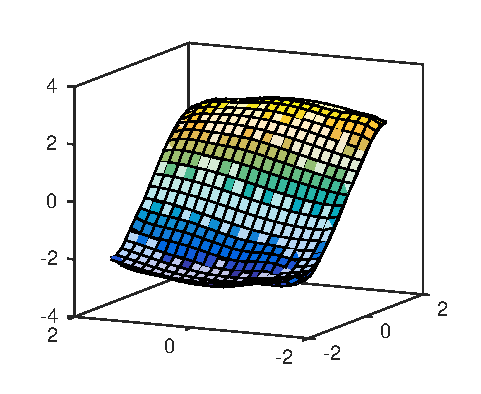
\includegraphics{plots/conclusions/robot_like/phi_approx.eps}
		%\caption{$\hat{W}_\varphi(t)$}
	\end{subfigure}
	\begin{subfigure}{0.5\textwidth}
		% This file was created by matlab2tikz.
%
\definecolor{mycolor1}{rgb}{0.00000,0.44700,0.74100}%
%
\begin{tikzpicture}

\begin{axis}[%
width=0.761\textwidth,
height=0.65\textwidth,
at={(0\textwidth,0\textwidth)},
scale only axis,
xmin=-2,
xmax=2,
ymin=0.06,
ymax=0.14,
axis background/.style={fill=white},
xmajorgrids,
ymajorgrids
]
\addplot [color=red, dashed, line width=1.2pt, forget plot]
  table[row sep=crcr]{%
-1.5707963267949	0.075\\
-1.55500942903816	0.0754735872604091\\
-1.53922253128143	0.0759470564929443\\
-1.5234356335247	0.0764202896991467\\
-1.50764873576797	0.0768931689393802\\
-1.49186183801123	0.0773655763622243\\
-1.4760749402545	0.0778373942338454\\
-1.46028804249777	0.0783085049673383\\
-1.44450114474104	0.0787787911520315\\
-1.4287142469843	0.0792481355827486\\
-1.41292734922757	0.0797164212890175\\
-1.39714045147084	0.080183531564223\\
-1.38135355371411	0.0806493499946915\\
-1.36556665595737	0.0811137604887046\\
-1.34977975820064	0.0815766473054307\\
-1.33399286044391	0.0820378950837711\\
-1.31820596268717	0.0824973888711092\\
-1.30241906493044	0.0829550141519604\\
-1.28663216717371	0.0834106568765104\\
-1.27084526941698	0.0838642034890401\\
-1.25505837166024	0.0843155409562251\\
-1.23927147390351	0.0847645567953064\\
-1.22348457614678	0.0852111391021234\\
-1.20769767839005	0.0856551765790028\\
-1.19191078063331	0.0860965585624964\\
-1.17612388287658	0.0865351750509603\\
-1.16033698511985	0.0869709167319702\\
-1.14455008736312	0.087403675009564\\
-1.12876318960638	0.0878333420313063\\
-1.11297629184965	0.0882598107151674\\
-1.09718939409292	0.0886829747762105\\
-1.08140249633619	0.0891027287530801\\
-1.06561559857945	0.0895189680342852\\
-1.04982870082272	0.0899315888842705\\
-1.03404180306599	0.0903404884692698\\
-1.01825490530925	0.090745564882934\\
-1.00246800755252	0.0911467171717286\\
-0.986681109795789	0.0915438453600932\\
-0.970894212039057	0.0919368504753575\\
-0.955107314282324	0.0923256345724077\\
-0.939320416525591	0.0927101007580959\\
-0.923533518768859	0.0930901532153884\\
-0.907746621012126	0.0934656972272454\\
-0.891959723255394	0.0938366392002258\\
-0.876172825498661	0.0942028866878132\\
-0.860385927741928	0.0945643484134556\\
-0.844599029985196	0.0949209342933129\\
-0.828812132228463	0.0952725554587083\\
-0.81302523447173	0.0956191242782755\\
-0.797238336714998	0.0959605543797992\\
-0.781451438958265	0.09629676067174\\
-0.765664541201532	0.0966276593644415\\
-0.7498776434448	0.0969531679910123\\
-0.734090745688067	0.0972732054278785\\
-0.718303847931335	0.0975876919150013\\
-0.702516950174602	0.0978965490757551\\
-0.686730052417869	0.0981996999364602\\
-0.670943154661137	0.0984970689455667\\
-0.655156256904404	0.0987885819924834\\
-0.639369359147671	0.0990741664260473\\
-0.623582461390939	0.0993537510726306\\
-0.607795563634206	0.0996272662538779\\
-0.592008665877474	0.0998946438040718\\
-0.576221768120741	0.100155817087121\\
-0.560434870364008	0.100410721013169\\
-0.544647972607276	0.100659292054812\\
-0.528861074850543	0.100901468262937\\
-0.513074177093811	0.101137189282154\\
-0.497287279337078	0.101366396365844\\
-0.481500381580345	0.101589032390796\\
-0.465713483823613	0.101805041871446\\
-0.44992658606688	0.102014370973703\\
-0.434139688310147	0.102216967528364\\
-0.418352790553415	0.102412781044123\\
-0.402565892796682	0.102601762720145\\
-0.386778995039949	0.102783865458235\\
-0.370992097283217	0.102959043874573\\
-0.355205199526484	0.103127254311025\\
-0.339418301769752	0.103288454846023\\
-0.323631404013019	0.103442605305015\\
-0.307844506256286	0.103589667270475\\
-0.292057608499554	0.103729604091478\\
-0.276270710742821	0.103862380892834\\
-0.260483812986088	0.103987964583781\\
-0.244696915229356	0.10410632386623\\
-0.228910017472623	0.104217429242566\\
-0.21312311971589	0.104321253023001\\
-0.197336221959158	0.104417769332472\\
-0.181549324202425	0.104506954117091\\
-0.165762426445693	0.10458878515014\\
-0.14997552868896	0.10466324203761\\
-0.134188630932227	0.104730306223284\\
-0.118401733175495	0.10478996099336\\
-0.102614835418762	0.10484219148062\\
-0.0868279376620293	0.10488698466813\\
-0.0710410399052968	0.10492432939249\\
-0.0552541421485642	0.104954216346611\\
-0.0394672443918316	0.104976638082038\\
-0.023680346635099	0.104991589010804\\
-0.00789344887836618	0.104999065406825\\
0.0078934488783664	0.104999065406825\\
0.023680346635099	0.104991589010804\\
0.0394672443918316	0.104976638082038\\
0.0552541421485642	0.104954216346611\\
0.071041039905297	0.10492432939249\\
0.0868279376620296	0.10488698466813\\
0.102614835418762	0.10484219148062\\
0.118401733175495	0.10478996099336\\
0.134188630932227	0.104730306223284\\
0.14997552868896	0.10466324203761\\
0.165762426445693	0.10458878515014\\
0.181549324202425	0.104506954117091\\
0.197336221959158	0.104417769332472\\
0.21312311971589	0.104321253023001\\
0.228910017472623	0.104217429242566\\
0.244696915229356	0.10410632386623\\
0.260483812986088	0.103987964583781\\
0.276270710742821	0.103862380892834\\
0.292057608499554	0.103729604091478\\
0.307844506256286	0.103589667270475\\
0.323631404013019	0.103442605305015\\
0.339418301769752	0.103288454846023\\
0.355205199526484	0.103127254311025\\
0.370992097283217	0.102959043874573\\
0.386778995039949	0.102783865458235\\
0.402565892796682	0.102601762720145\\
0.418352790553415	0.102412781044123\\
0.434139688310147	0.102216967528364\\
0.44992658606688	0.102014370973703\\
0.465713483823612	0.101805041871446\\
0.481500381580345	0.101589032390796\\
0.497287279337078	0.101366396365844\\
0.51307417709381	0.101137189282154\\
0.528861074850543	0.100901468262937\\
0.544647972607275	0.100659292054812\\
0.560434870364008	0.100410721013169\\
0.576221768120741	0.100155817087121\\
0.592008665877473	0.0998946438040718\\
0.607795563634206	0.0996272662538779\\
0.623582461390939	0.0993537510726306\\
0.639369359147671	0.0990741664260473\\
0.655156256904404	0.0987885819924834\\
0.670943154661137	0.0984970689455667\\
0.686730052417869	0.0981996999364602\\
0.702516950174602	0.0978965490757551\\
0.718303847931335	0.0975876919150013\\
0.734090745688067	0.0972732054278785\\
0.7498776434448	0.0969531679910123\\
0.765664541201533	0.0966276593644415\\
0.781451438958265	0.09629676067174\\
0.797238336714998	0.0959605543797992\\
0.81302523447173	0.0956191242782755\\
0.828812132228463	0.0952725554587083\\
0.844599029985196	0.0949209342933129\\
0.860385927741928	0.0945643484134556\\
0.876172825498661	0.0942028866878132\\
0.891959723255393	0.0938366392002258\\
0.907746621012126	0.0934656972272454\\
0.923533518768859	0.0930901532153884\\
0.939320416525591	0.0927101007580959\\
0.955107314282324	0.0923256345724077\\
0.970894212039056	0.0919368504753575\\
0.986681109795789	0.0915438453600932\\
1.00246800755252	0.0911467171717287\\
1.01825490530925	0.090745564882934\\
1.03404180306599	0.0903404884692698\\
1.04982870082272	0.0899315888842705\\
1.06561559857945	0.0895189680342852\\
1.08140249633619	0.0891027287530801\\
1.09718939409292	0.0886829747762105\\
1.11297629184965	0.0882598107151674\\
1.12876318960638	0.0878333420313063\\
1.14455008736312	0.087403675009564\\
1.16033698511985	0.0869709167319702\\
1.17612388287658	0.0865351750509603\\
1.19191078063331	0.0860965585624964\\
1.20769767839005	0.0856551765790029\\
1.22348457614678	0.0852111391021234\\
1.23927147390351	0.0847645567953063\\
1.25505837166024	0.0843155409562251\\
1.27084526941698	0.0838642034890401\\
1.28663216717371	0.0834106568765104\\
1.30241906493044	0.0829550141519604\\
1.31820596268717	0.0824973888711093\\
1.33399286044391	0.0820378950837711\\
1.34977975820064	0.0815766473054308\\
1.36556665595737	0.0811137604887046\\
1.38135355371411	0.0806493499946915\\
1.39714045147084	0.080183531564223\\
1.41292734922757	0.0797164212890175\\
1.4287142469843	0.0792481355827485\\
1.44450114474104	0.0787787911520315\\
1.46028804249777	0.0783085049673383\\
1.4760749402545	0.0778373942338454\\
1.49186183801123	0.0773655763622243\\
1.50764873576797	0.0768931689393802\\
1.5234356335247	0.0764202896991467\\
1.53922253128143	0.0759470564929443\\
1.55500942903816	0.0754735872604091\\
1.5707963267949	0.075\\
};
\addplot [color=mycolor1, line width=1.2pt, forget plot]
  table[row sep=crcr]{%
-1.5707963267949	0.13894275301251\\
-1.55500942903816	0.133466793484962\\
-1.53922253128143	0.128276225727673\\
-1.5234356335247	0.123372183242448\\
-1.50764873576797	0.118754657183281\\
-1.49186183801123	0.114422544385183\\
-1.4760749402545	0.110373703231876\\
-1.46028804249777	0.106605016480154\\
-1.44450114474104	0.103112460081218\\
-1.4287142469843	0.0998911769771022\\
-1.41292734922757	0.0969355548046311\\
-1.39714045147084	0.0942393064107406\\
-1.38135355371411	0.0917955520719252\\
-1.36556665595737	0.0895969023170682\\
-1.34977975820064	0.087635540276733\\
-1.33399286044391	0.0859033025225723\\
-1.31820596268717	0.0843917574169652\\
-1.30241906493044	0.0830922800641514\\
-1.28663216717371	0.0819961230385676\\
-1.27084526941698	0.0810944821621218\\
-1.25505837166024	0.0803785567078866\\
-1.23927147390351	0.0798396035211165\\
-1.22348457614678	0.0794689846673977\\
-1.20769767839005	0.0792582083398996\\
-1.19191078063331	0.0791989628807935\\
-1.17612388287658	0.0792831438936763\\
-1.16033698511985	0.0795028745420554\\
-1.14455008736312	0.0798505192414914\\
-1.12876318960638	0.0803186910578961\\
-1.11297629184965	0.0809002532199383\\
-1.09718939409292	0.0815883152379655\\
-1.08140249633619	0.082376224193975\\
-1.06561559857945	0.0832575518259245\\
-1.04982870082272	0.0842260780743101\\
-1.03404180306599	0.0852757717890113\\
-1.01825490530925	0.0864007693097763\\
-1.00246800755252	0.0875953516345707\\
-0.986681109795789	0.0888539208768135\\
-0.970894212039057	0.090170976686037\\
-0.955107314282324	0.0915410932677531\\
-0.939320416525591	0.0929588975885488\\
-0.923533518768859	0.0944190492931305\\
-0.907746621012126	0.0959162227928204\\
-0.891959723255394	0.0974450919116309\\
-0.876172825498661	0.0990003173983588\\
-0.860385927741928	0.100576537533015\\
-0.844599029985196	0.102168361975234\\
-0.828812132228463	0.103770368922895\\
-0.81302523447173	0.105377105572841\\
-0.797238336714998	0.106983091803792\\
-0.781451438958265	0.108582826935939\\
-0.765664541201532	0.110170799363365\\
-0.7498776434448	0.111741498805519\\
-0.734090745688067	0.113289430883199\\
-0.718303847931335	0.114809133693468\\
-0.702516950174602	0.116295196036875\\
-0.686730052417869	0.117742276939276\\
-0.670943154661137	0.119145126109303\\
-0.655156256904404	0.120498604980468\\
-0.639369359147671	0.121797708003448\\
-0.623582461390939	0.123037583878218\\
-0.607795563634206	0.124213556446392\\
-0.592008665877474	0.125321145000072\\
-0.576221768120741	0.126356083803368\\
-0.560434870364008	0.127314340665119\\
-0.544647972607276	0.128192134444759\\
-0.528861074850543	0.128985951416232\\
-0.513074177093811	0.129692560456105\\
-0.497287279337078	0.130309027060037\\
-0.481500381580345	0.130832726225561\\
-0.465713483823613	0.131261354267542\\
-0.44992658606688	0.131592939654849\\
-0.434139688310147	0.131825852972152\\
-0.418352790553415	0.13195881611876\\
-0.402565892796682	0.131990910856973\\
-0.386778995039949	0.131921586815446\\
-0.370992097283217	0.131750669038937\\
-0.355205199526484	0.131478365154909\\
-0.339418301769752	0.131105272200553\\
-0.323631404013019	0.130632383121818\\
-0.307844506256286	0.130061092919913\\
-0.292057608499554	0.129393204381866\\
-0.276270710742821	0.128630933291246\\
-0.260483812986088	0.127776912974569\\
-0.244696915229356	0.126834197999556\\
-0.228910017472623	0.12580626680478\\
-0.21312311971589	0.124697023007626\\
-0.197336221959158	0.123510795110228\\
-0.181549324202425	0.122252334302292\\
-0.165762426445693	0.120926810046504\\
-0.14997552868896	0.119539803127316\\
-0.134188630932227	0.118097295848056\\
-0.118401733175495	0.116605659074808\\
-0.102614835418762	0.115071635848593\\
-0.0868279376620293	0.113502321319907\\
-0.0710410399052968	0.111905138801396\\
-0.0552541421485642	0.11028781178466\\
-0.0394672443918316	0.108658331825191\\
-0.023680346635099	0.10702492226413\\
-0.00789344887836618	0.105395997825727\\
0.0078934488783664	0.103780120203642\\
0.023680346635099	0.102185949826006\\
0.0394672443918316	0.100622194066937\\
0.0552541421485642	0.0990975522490777\\
0.071041039905297	0.0976206578561967\\
0.0868279376620296	0.0962000184450974\\
0.102614835418762	0.0948439538104712\\
0.118401733175495	0.0935605330133254\\
0.134188630932227	0.0923575109318338\\
0.14997552868896	0.0912422650316635\\
0.165762426445693	0.0902217330799923\\
0.181549324202425	0.0893023525427718\\
0.197336221959158	0.0884900024077368\\
0.21312311971589	0.0877899481659605\\
0.228910017472623	0.0872067906623783\\
0.244696915229356	0.0867444194909208\\
0.260483812986088	0.0864059715632517\\
0.276270710742821	0.08619379542239\\
0.292057608499554	0.0861094218047354\\
0.307844506256286	0.0861535408774857\\
0.323631404013019	0.0863259864945588\\
0.339418301769752	0.086625727724523\\
0.355205199526484	0.0870508678104246\\
0.370992097283217	0.0875986506255542\\
0.386778995039949	0.0882654745930031\\
0.402565892796682	0.0890469139421115\\
0.418352790553415	0.0899377470834325\\
0.434139688310147	0.0909319917973197\\
0.44992658606688	0.0920229468512672\\
0.465713483823612	0.093203239589109\\
0.481500381580345	0.0944648789723591\\
0.497287279337078	0.0957993135013131\\
0.51307417709381	0.0971974934018332\\
0.528861074850543	0.098649936433488\\
0.544647972607275	0.100146796656143\\
0.560434870364008	0.101677935485185\\
0.576221768120741	0.103232994369983\\
0.592008665877473	0.104801468445434\\
0.607795563634206	0.106372780531625\\
0.623582461390939	0.107936354890867\\
0.639369359147671	0.109481690193307\\
0.655156256904404	0.110998431190714\\
0.670943154661137	0.112476438651343\\
0.686730052417869	0.113905857165426\\
0.702516950174602	0.115277180489281\\
0.718303847931335	0.116581314154541\\
0.734090745688067	0.117809635126115\\
0.7498776434448	0.118954048346686\\
0.765664541201533	0.120007040055364\\
0.781451438958265	0.120961727812497\\
0.797238336714998	0.121811907200373\\
0.81302523447173	0.12255209519992\\
0.828812132228463	0.123177570265926\\
0.844599029985196	0.123684409137278\\
0.860385927741928	0.124069520424393\\
0.876172825498661	0.124330675013282\\
0.891959723255393	0.124466533315178\\
0.907746621012126	0.124476669372898\\
0.923533518768859	0.124361591811033\\
0.939320416525591	0.124122761587704\\
0.955107314282324	0.123762606472299\\
0.970894212039056	0.123284532137631\\
0.986681109795789	0.122692929717909\\
1.00246800755252	0.121993179647277\\
1.01825490530925	0.121191651559096\\
1.03404180306599	0.120295699995147\\
1.04982870082272	0.119313655648068\\
1.06561559857945	0.118254811840978\\
1.08140249633619	0.11712940593663\\
1.09718939409292	0.115948595365823\\
1.11297629184965	0.114724427971799\\
1.12876318960638	0.113469806384947\\
1.14455008736312	0.112198446170468\\
1.16033698511985	0.110924827530997\\
1.17612388287658	0.109664140396406\\
1.19191078063331	0.108432222793616\\
1.20769767839005	0.107245492459626\\
1.22348457614678	0.106120871740127\\
1.23927147390351	0.105075705902842\\
1.25505837166024	0.104127675087628\\
1.27084526941698	0.103294700212872\\
1.28663216717371	0.102594843257969\\
1.30241906493044	0.102046202442778\\
1.31820596268717	0.101666802924981\\
1.33399286044391	0.101474483733132\\
1.34977975820064	0.101486781744902\\
1.36556665595737	0.101720813604582\\
1.38135355371411	0.102193156549439\\
1.39714045147084	0.102919729179279\\
1.41292734922757	0.103915673255942\\
1.4287142469843	0.105195237658032\\
1.44450114474104	0.106771665639965\\
1.46028804249777	0.108657086552247\\
1.4760749402545	0.110862413171523\\
1.49186183801123	0.113397245763688\\
1.50764873576797	0.116269783961546\\
1.5234356335247	0.11948674748025\\
1.53922253128143	0.123053306619698\\
1.55500942903816	0.126973023414203\\
1.5707963267949	0.131247804187111\\
};
\end{axis}
\end{tikzpicture}%
		%\caption{$\hat{W}_\gamma(t)$)}
	\end{subfigure}
	\caption{Προσεγγίσεις των συναρτήσεων $\varphi(x)$ (αριστερά) και $\gamma(x)$ (δεξιά) στο παράδειγμα \ref{subsec:robot_like_init_approach}}
	\label{fig:robot_like_approximations}
\end{figure}

\pagebreak

{
	\begin{wrapfigure}{r}{0.4\textwidth}
		%\centering
		% This file was created by matlab2tikz.
%
\definecolor{mycolor1}{rgb}{0.00000,0.44700,0.74100}%
%
\begin{tikzpicture}

\begin{axis}[%
width=0.3\textwidth,
height=0.288\textwidth,
at={(0\textwidth,0\textwidth)},
scale only axis,
xmin=-3.5,
xmax=3.5,
xlabel style={font=\color{white!15!black}},
xlabel={$x_1$},
ymin=-3.5,
ymax=3.5,
ylabel style={font=\color{white!15!black}},
ylabel={$x_2$},
axis background/.style={fill=white},
xmajorgrids,
ymajorgrids
]
\addplot [color=red, line width=1.5pt, draw=none, mark=x, mark options={solid, red}, forget plot]
  table[row sep=crcr]{%
-1.5707963267949	-1.5707963267949\\
-1.5707963267949	-0.942477796076938\\
-1.5707963267949	-0.314159265358979\\
-1.5707963267949	0.314159265358979\\
-1.5707963267949	0.942477796076938\\
-1.5707963267949	1.5707963267949\\
-0.942477796076938	-1.5707963267949\\
-0.942477796076938	-0.942477796076938\\
-0.942477796076938	-0.314159265358979\\
-0.942477796076938	0.314159265358979\\
-0.942477796076938	0.942477796076938\\
-0.942477796076938	1.5707963267949\\
-0.314159265358979	-1.5707963267949\\
-0.314159265358979	-0.942477796076938\\
-0.314159265358979	-0.314159265358979\\
-0.314159265358979	0.314159265358979\\
-0.314159265358979	0.942477796076938\\
-0.314159265358979	1.5707963267949\\
0.314159265358979	-1.5707963267949\\
0.314159265358979	-0.942477796076938\\
0.314159265358979	-0.314159265358979\\
0.314159265358979	0.314159265358979\\
0.314159265358979	0.942477796076938\\
0.314159265358979	1.5707963267949\\
0.942477796076938	-1.5707963267949\\
0.942477796076938	-0.942477796076938\\
0.942477796076938	-0.314159265358979\\
0.942477796076938	0.314159265358979\\
0.942477796076938	0.942477796076938\\
0.942477796076938	1.5707963267949\\
1.5707963267949	-1.5707963267949\\
1.5707963267949	-0.942477796076938\\
1.5707963267949	-0.314159265358979\\
1.5707963267949	0.314159265358979\\
1.5707963267949	0.942477796076938\\
1.5707963267949	1.5707963267949\\
};
\addplot [color=mycolor1, line width=1.5pt, draw=none, mark=o, mark options={solid, mycolor1}, forget plot]
  table[row sep=crcr]{%
-2.82743338823081	-2.82743338823081\\
-2.82743338823081	-2.19911485751286\\
-2.82743338823081	-1.5707963267949\\
-2.82743338823081	-0.942477796076938\\
-2.82743338823081	-0.314159265358979\\
-2.82743338823081	0.314159265358979\\
-2.82743338823081	0.942477796076938\\
-2.82743338823081	1.5707963267949\\
-2.82743338823081	2.19911485751286\\
-2.82743338823081	2.82743338823081\\
-2.19911485751286	-2.82743338823081\\
-2.19911485751286	-2.19911485751286\\
-2.19911485751286	-1.5707963267949\\
-2.19911485751286	-0.942477796076938\\
-2.19911485751286	-0.314159265358979\\
-2.19911485751286	0.314159265358979\\
-2.19911485751286	0.942477796076938\\
-2.19911485751286	1.5707963267949\\
-2.19911485751286	2.19911485751286\\
-2.19911485751286	2.82743338823081\\
-1.5707963267949	-2.82743338823081\\
-1.5707963267949	-2.19911485751286\\
-1.5707963267949	2.19911485751286\\
-1.5707963267949	2.82743338823081\\
-0.942477796076938	-2.82743338823081\\
-0.942477796076938	-2.19911485751286\\
-0.942477796076938	2.19911485751286\\
-0.942477796076938	2.82743338823081\\
-0.314159265358979	-2.82743338823081\\
-0.314159265358979	-2.19911485751286\\
-0.314159265358979	2.19911485751286\\
-0.314159265358979	2.82743338823081\\
0.314159265358979	-2.82743338823081\\
0.314159265358979	-2.19911485751286\\
0.314159265358979	2.19911485751286\\
0.314159265358979	2.82743338823081\\
0.942477796076938	-2.82743338823081\\
0.942477796076938	-2.19911485751286\\
0.942477796076938	2.19911485751286\\
0.942477796076938	2.82743338823081\\
1.5707963267949	-2.82743338823081\\
1.5707963267949	-2.19911485751286\\
1.5707963267949	2.19911485751286\\
1.5707963267949	2.82743338823081\\
2.19911485751286	-2.82743338823081\\
2.19911485751286	-2.19911485751286\\
2.19911485751286	-1.5707963267949\\
2.19911485751286	-0.942477796076938\\
2.19911485751286	-0.314159265358979\\
2.19911485751286	0.314159265358979\\
2.19911485751286	0.942477796076938\\
2.19911485751286	1.5707963267949\\
2.19911485751286	2.19911485751286\\
2.19911485751286	2.82743338823081\\
2.82743338823081	-2.82743338823081\\
2.82743338823081	-2.19911485751286\\
2.82743338823081	-1.5707963267949\\
2.82743338823081	-0.942477796076938\\
2.82743338823081	-0.314159265358979\\
2.82743338823081	0.314159265358979\\
2.82743338823081	0.942477796076938\\
2.82743338823081	1.5707963267949\\
2.82743338823081	2.19911485751286\\
2.82743338823081	2.82743338823081\\
};
\end{axis}
\end{tikzpicture}%
		\captionsetup{format=plain}
		\caption{Επαυξημένο πλέγμα. Τα αρχικά κέντρα συμβολίζονται με κόκκινο, ενώ τα νέα με μπλε.}
		\label{fig:aug_phase_plain}	
	\end{wrapfigure}

\subsection{Επέκταση του πλέγματος αναγνώρισης}
\label{subsec:extended_grid}
Προς την βελτίωση των παραπάνω αποτελεσμάτων, το πλέγμα επαυξάνεται προσθέτοντας γκαουσιανές εκτός του συνόλου $\Omega_x$, σύμφωνα με την Παρατήρηση \ref{remakr:border_eval}. Τα νέα κέντρα  $c_\Phi$ και $c_\gamma$ θα ανήκουν στα σύνολα:
\begin{equation*}
\mathcal{C}_\Phi = \bigtimes\limits_{i=1}^{2}  \begin{Bmatrix}
-\frac{3\pi}{4} + \frac{\pi}{5} k, \quad  k = 0,1,\dots,9
\end{Bmatrix}
\end{equation*}
και
\begin{equation*}
\mathcal{C}_\Gamma = \begin{Bmatrix}
-\frac{3\pi}{4} + \frac{\pi}{5} k, \quad  k = 0,1,\dots,9
\end{Bmatrix}
\end{equation*}
δηλαδή θα προσεγγίσουμε τις άγνωστες συναρτήσεις στο χωρίο $D = \bmqty{-\frac{3\pi}{4},\frac{3\pi}{4}}^2$ το οποίο είναι υπερσύνολο του $\Omega_x$. Το νέο επαυξημένο πλέγμα φαίνεται στο Σχήμα \ref{fig:aug_phase_plain}. Τα κέρδη του νέου σχήματος αναγνώρισης επιλέγονται ίσα με αυτά του αρχικού σχήματος, και δίνονται στον Πίνακα \ref{tab:robot_equiv_schema_params}.

}

\subsubsection{Αποτελέσματα}
Το σύστημα κλειστού βρόγχου με τα επαυξημένα νευρωνικά δίκτυα RBF προσομοιώθηκε για 100 επαναλήψεις. Στο Σχήμα \ref{fig:robot_like_extended_w_conv} δίνεται η χρονική εξέλιξη κάποιων βαρών $\hat{\varphi}(t)$ και $\hat{\gamma}(t)$, απ' όπου είναι προφανές πως τα βάρη έχουν σταθεροποιηθεί. Αρχικά σημειώνουμε πως σε αυτό το πείραμα τα βάρη σταθεροποιούνται πολύ πιο γρήγορα από το προηγούμενο πείραμα, και καθώς τα κέρδη $\beta_\varphi$ και $\beta_\gamma$ είναι τα ίδια, συμπεραίνουμε πως αυτό οφείλεται σε μεγαλύτερα επίπεδα διέγερσης.

Στην συνέχεια, στο 
Σχήμα \ref{fig:robot_like_extended_approximations} φαίνονται οι προσεγγίσεις των συναρτήσεων στο σύνολο $\Omega_x$. Όπως φαίνεται λοιπόν οι τροποποιήσεις που εφαρμόσαμε πράγματι είχαν αποτελέσματα. Ενώ η προσέγγιση της $\varphi(x)$ είναι και στις δυο περιπτώσεις πολύ ικανοποιητική, στο νέο επαυξημένο σχήμα τα αποτελέσματα αναγνώρισης της $\gamma(x)$ είναι πολύ καλύτερα. Φυσικά από το σχήμα φαίνεται πως τα αποτελέσματα για $x_1 > 1$ επιδέχονται βελτίωση, αλλά και πάλι τα αποτελέσματα αυτά αποτελούν τεράστια βελτίωση σε σύγκριση με τα αποτελέσματα της Ενότητας \ref{subsec:robot_like_init_approach}.

%Όπως φαίνεται λοιπόν και από τα αποτελέσματα, οι τροποποιήσεις που εφαρμόσαμε πράγματι είχαν αποτελέσματα. Ενώ η προσέγγιση της $f(x)$ είναι και στις 2 περιπτώσεις πολυ ικανοποιητική, σε αυτή την σειρά πειραμάτων φαίνεται πως καραφέραμε να βελτιώσουμε τόσο πολύ τα αποτελέσματα που πλέον είναι εφικτή και η αναγνώριση της $g(x)$ όπως φαίνεται και στο σχήμα $( \ref{fig:f_g_approx_dense_grid_experiments} )$. Φυσικά από το σχήμα φαίνεται πως τα αποτελέσματα κοντά στην γωνία $+\pi/2$ επιδέχονται βελτίωση, αλλά και πάλι τα αποτελέσματα αυτά αποτελούν τεράστια βελτίωση.

\begin{figure}
	\begin{subfigure}{0.5\textwidth}
		% This file was created by matlab2tikz.
%
\definecolor{mycolor1}{rgb}{0.00000,0.44700,0.74100}%
\definecolor{mycolor2}{rgb}{0.85000,0.32500,0.09800}%
\definecolor{mycolor3}{rgb}{0.92900,0.69400,0.12500}%
\definecolor{mycolor4}{rgb}{0.49400,0.18400,0.55600}%
\definecolor{mycolor5}{rgb}{0.46600,0.67400,0.18800}%
%
\begin{tikzpicture}

\begin{axis}[%
width=0.761\textwidth,
height=0.65\textwidth,
at={(0\textwidth,0\textwidth)},
scale only axis,
xmin=0,
xmax=20000,
xlabel style={font=\color{white!15!black}},
xlabel={Time, $t$},
ymin=-1,
ymax=0.2,
ylabel style={font=\color{white!15!black}},
ylabel={$\hat{W}_\varphi(t)$},
axis background/.style={fill=white},
xmajorgrids,
ymajorgrids
]
\addplot [color=mycolor1, line width=1.2pt, forget plot]
  table[row sep=crcr]{%
0	0\\
17.2393573816189	-0.00561802086303942\\
35.4784084120474	-0.0199823223847488\\
57.0857438913881	-0.0384395490182214\\
77.1282094703602	-0.0509270548282075\\
95.9404941721004	-0.0539825713676692\\
113.690551411986	-0.0480742113795714\\
135.856587340397	-0.0329175067308825\\
157.746727439138	-0.0145313550056017\\
178.214212013121	-0.00134151898237178\\
200	0.00201370022841729\\
224.013024770462	0.00454349488791195\\
251.375961509999	5.99657141719945e-05\\
276.001511991471	-0.0054758904807386\\
298.316011324176	-0.00945985699217999\\
323.065760113845	-0.00978572020903812\\
352.259618747892	-0.0065945890310104\\
377.227228097672	-0.00201926556837861\\
398.295418384809	-0.00229663329446339\\
421.309807588557	0.000875783731316915\\
449.968869313376	-0.00126578719573445\\
500.401284361695	-0.00378185830777511\\
551.554816988202	-0.00288493645348353\\
578	-0.00102921134021017\\
600.826076064186	-0.00233383180966484\\
625.763667398216	-0.000538757114554755\\
682.529269521816	-0.00237924440079951\\
736.761257292706	-0.00275311926452559\\
764.000704241971	-0.00221902700286591\\
790.681266361094	-0.00280863002262777\\
814.01799914267	-0.00118236482376233\\
918.572619838989	-0.00287199605736532\\
944.061571791484	-0.00219083391857566\\
972.431273784896	-0.00212022625782993\\
998.356454470919	-0.00353343628376024\\
1020.00158592428	-0.00115297308002482\\
1045.18736527428	-0.00273380212092889\\
1104	-0.00292447382889804\\
1162	-0.003196051082341\\
1185.60671813412	-0.00403592206203029\\
1207.90008849559	-0.002970921996166\\
1234.63891839598	-0.00266523977552424\\
1262.29466991384	-0.00337253705583862\\
1322.14050570113	-0.00324585878843209\\
1379.6899166213	-0.00309632684002281\\
1402.33176594204	-0.00432276846549939\\
1427.73343768224	-0.00319756374665303\\
1489.65536198976	-0.00392436214679037\\
1552.18869164796	-0.00378688116688863\\
1580.17145858851	-0.00360656901102629\\
1605.65966130913	-0.00433754310870427\\
1636	-0.00392495654159575\\
1698.44508354652	-0.00435225563342101\\
1729.15942441455	-0.00431516246317187\\
1761.67831725529	-0.00477463100105524\\
1788.14668784458	-0.00563694479569676\\
1817.61815985952	-0.00400121442726231\\
1844.73839020713	-0.00484785428488976\\
1966.43446211382	-0.00504922000254737\\
1997.33226583417	-0.00622133938304614\\
2023.03049589416	-0.0046265193450381\\
2054.46075772411	-0.00523419043020112\\
2176.12473270708	-0.00532481286791153\\
2202.35990349432	-0.00618893965656753\\
2232.28258129956	-0.005368863712647\\
2294.96892215966	-0.00570942457125057\\
2355.62650682947	-0.00571670221324894\\
2384.08787696778	-0.00697851201039157\\
2413.74093050014	-0.00589882334315917\\
2441.76690698773	-0.00626449511037208\\
2537.3287483013	-0.00617683948075864\\
2565.09553705123	-0.0065271284620394\\
2596.39239710208	-0.00757850413720007\\
2623.95640256362	-0.00608232708327705\\
2654.35292696457	-0.00659815893959603\\
2776.75459241781	-0.00670587206695927\\
2804.86208261916	-0.00717846857878612\\
2835.05837436335	-0.00678941015576129\\
2924.32792724651	-0.00708056094663334\\
2956.38569781028	-0.00705308360193158\\
2984.66427859967	-0.00828237272799015\\
3013.44392718815	-0.00722165063780267\\
3042.00042699522	-0.0075922400719719\\
3132.69623161236	-0.00746848193375627\\
3164.00047733373	-0.00782878115933272\\
3195.46178492226	-0.00878569938140572\\
3222.73884027407	-0.00740370134008117\\
3252.2751289859	-0.00786540892659104\\
3373.23927768387	-0.00802840695541818\\
3401.99352345592	-0.00866288528413861\\
3430.75169220074	-0.00800282185082324\\
3522.78084300893	-0.00826737095485441\\
3553.85914354451	-0.00828476147216861\\
3582.83079616623	-0.00956763829526608\\
3609.93835386302	-0.00856095302879112\\
3762.12077612657	-0.00899948986625532\\
3791.06827541159	-0.00987943686777726\\
3819.59603769375	-0.00834985509209218\\
3848.02498423146	-0.00905633406364359\\
3972.0068838915	-0.00922150655242149\\
4000.00178284955	-0.0101747967310075\\
4027.80169056695	-0.00915224574782769\\
4148.6428913196	-0.00946266961909714\\
4360.05638522758	-0.00979922141050338\\
4388.20829081911	-0.0109147319963085\\
4416.76840344911	-0.00971366197336465\\
4446.33767010058	-0.0100990320970595\\
4539.04164147877	-0.0100744484734605\\
4567.93321889851	-0.0103768995650171\\
4597.53077007673	-0.0112597928018658\\
4624.57675389689	-0.0101593473809771\\
4685.45645549934	-0.0103848775870574\\
4775.98189722807	-0.0105877406203945\\
4802.06837463594	-0.0110391400921799\\
4832.18201882145	-0.0105328256286157\\
4922.08268650165	-0.0107346917720861\\
4954.25118599657	-0.0107693447862403\\
4983.88278561754	-0.0118677135578764\\
5011.20653319127	-0.0108867899070901\\
5072.14705410111	-0.0109885767997184\\
5130.95395231154	-0.0110380343285215\\
5162.1875380442	-0.0113481790322112\\
5190.72393092837	-0.0121553051649244\\
5218.67674876614	-0.0108934459567536\\
5248.01380481388	-0.0113680618414946\\
5340.61216002635	-0.0113690351863625\\
5370	-0.0116119769772922\\
5398.66717206488	-0.0123861419742752\\
5427.42397132655	-0.0114628840492514\\
5606.05731467401	-0.0120340131579724\\
5698.67054761995	-0.0117975910252426\\
5759.50080845834	-0.0120047732161765\\
5787.48354305518	-0.0129990523200831\\
5816.29553553057	-0.0118589765879733\\
5845.32163566092	-0.0122272930384497\\
5938.13056981319	-0.0122003439755645\\
5966.76781288947	-0.0125162165495567\\
5995.31840518939	-0.0133048509451328\\
6021.57218322128	-0.0120301642200502\\
6053.04219600811	-0.0124717903963756\\
6174.42092072442	-0.0126705038819637\\
6199.62198380927	-0.0134514975834463\\
6227.11949210105	-0.0125628602181678\\
6403.91014989882	-0.0131492644286482\\
6432.96802539271	-0.0127564482281741\\
6523.28811417275	-0.0129819827234314\\
6555.35432772865	-0.0130185819325561\\
6582.5661188509	-0.0141758973695687\\
6606.03514580354	-0.0133277809218271\\
6666.40430147764	-0.0132181901935837\\
6759.45883276799	-0.0133010719910089\\
6784.6559155886	-0.0143315684945264\\
6808	-0.0134885971310723\\
6898.74776553134	-0.0133577726228395\\
6958.53676670662	-0.0135529262261116\\
6982.82981590144	-0.0146899394676439\\
7004	-0.0139136183424853\\
7033.29369821809	-0.0135431953349325\\
7125.93584470204	-0.0137759767385432\\
7158.42424976384	-0.0137912192185468\\
7182.03046327424	-0.0148878540239821\\
7202.01503348863	-0.0141783116814622\\
7231.73123090142	-0.0138085784456052\\
7322.18983661845	-0.0139799421813223\\
7378.55860507845	-0.0141753454045102\\
7400.26926171925	-0.0148644419059565\\
7426.00414726255	-0.0140521050961979\\
7598.1843582013	-0.0152364074820071\\
7624.00489654455	-0.0142318090074696\\
7686.79894332197	-0.0144047965186473\\
7775.59997035877	-0.0146715577648138\\
7798.23461787805	-0.0154728387897194\\
7822.3257406313	-0.0143740875682852\\
7884.39508298325	-0.0146651608629327\\
7973.79490961509	-0.014945097387681\\
7997.68644575285	-0.0157322479826689\\
8024.0042603134	-0.0147167480499775\\
8084.20669189152	-0.0149083063661237\\
8173.60554326937	-0.0151718599699961\\
8198	-0.0159393811336486\\
8224.00548272074	-0.0149513547657989\\
8284.33324500063	-0.0151430722507939\\
8375.74782149459	-0.0153972565385629\\
8399.7440819163	-0.016089036136691\\
8424.92498090623	-0.0152570951504458\\
8578.34542438943	-0.0156549256753351\\
8601.30582058407	-0.0153002270453726\\
8660.66664075589	-0.0156975010650058\\
8754.00058570121	-0.0157344254039344\\
8783.20159837654	-0.0168612866000331\\
8808.15701993729	-0.0159009766794043\\
8899.70678452284	-0.0157855154211575\\
8960	-0.0160040718037635\\
8987.60754182848	-0.0169309522025287\\
9014.42375359506	-0.0159139292954933\\
9074.14175333708	-0.0160919957961596\\
9166.08783891718	-0.0164900657910039\\
9194.60341725689	-0.0171344335940375\\
9221.10847786595	-0.0160467093082843\\
9248.48402425966	-0.0164065252174623\\
9340.9595050028	-0.0164858223397459\\
9369.63411914081	-0.0166770363612159\\
9397.8921016656	-0.0173503301230085\\
9423.23311312012	-0.0163476605557662\\
9483.02520893466	-0.0165435093913402\\
9574.40886243652	-0.0168174693280889\\
9600.84464899031	-0.0170707356519415\\
9627.59926791431	-0.01668166498348\\
9803.39422159789	-0.0170910507331428\\
9859.3839283079	-0.0169994946700172\\
9952.57910825104	-0.0170927947801829\\
9982.86002866336	-0.0181992661782715\\
10008.3158748529	-0.0171942362758273\\
10096.9232095916	-0.0171054843740421\\
10157.1661291676	-0.0172717501955049\\
10184.6821894411	-0.0182608366449131\\
10210.2590969847	-0.0173312848128262\\
10330.5043270316	-0.0174617363809375\\
10388.4189238783	-0.0184341115818825\\
10414.7063835672	-0.0174313625066134\\
10472.6927305533	-0.0175771939357219\\
10565.2236653125	-0.017959712058655\\
10595.5834531727	-0.0185780582687585\\
10621.5579397516	-0.0175119615196309\\
10681.2884977442	-0.0177880343217112\\
10774.0024457096	-0.0180835457176727\\
10800.4727845328	-0.0184884979971685\\
10824.6606744162	-0.0179176509154786\\
11002.6698298135	-0.0183391709360876\\
11058.3304012213	-0.0182712303758308\\
11149.5250287809	-0.0184108833782375\\
11260	-0.0185049627216358\\
11350.7883457083	-0.0186048019277223\\
11382.0769109422	-0.0196187215587997\\
11408.0089418715	-0.0186767009545292\\
11497.9645430047	-0.0185757827821362\\
11558.5399863382	-0.0187645347978105\\
11586.7134563315	-0.0196899351503816\\
11614.5425424958	-0.0186813976979465\\
11670	-0.0188580421854567\\
11762.3261171677	-0.0192042148773908\\
11789.3403790637	-0.0198365855103475\\
11815.4957744361	-0.0187932316985098\\
11870.2355865028	-0.0190554641121707\\
11963.0877021383	-0.0193902684404748\\
11991.1973774368	-0.0200440691951371\\
12017.6403157699	-0.0188956718011468\\
12042.8831874315	-0.0192702083513723\\
12136.2011972348	-0.0193256721868238\\
12195.5057075678	-0.0202349370556476\\
12221.2223146225	-0.0191743341420079\\
12246.529152494	-0.0194991726530134\\
12338.9773950051	-0.0195402134377218\\
12397.3397237648	-0.0203662690000783\\
12422.6674580851	-0.0194213461327308\\
12481.1279785493	-0.0195794335049868\\
12570.0468725412	-0.0199373186442244\\
12599.4632976122	-0.0204440242341661\\
12624.1715955111	-0.0196691623496008\\
12772.5897078961	-0.0201112522445328\\
12826.3286375593	-0.0199139742107945\\
13002.7804113526	-0.0203222670170362\\
13059.1020296629	-0.0202643521006394\\
13118.1122085133	-0.0201458810624899\\
13179.8859547725	-0.0205090818526514\\
13354.2499250479	-0.020488180758548\\
13382.9095122161	-0.0216078861994902\\
13409.0928417275	-0.0205035224353196\\
13557.0840415163	-0.0206773655190773\\
13585.9134775615	-0.0216275776147086\\
13614.2464745962	-0.0205673514865339\\
13670	-0.0207624250579101\\
13760.3530219967	-0.0208823372668121\\
13789.5436595187	-0.021746320384409\\
13816.96395378	-0.0207200726908923\\
13874.8637470359	-0.0209162279097654\\
13965.0397751667	-0.0213125554182625\\
13995.0773679604	-0.021902929420321\\
14019.9776797273	-0.0208612208116392\\
14045.0992544779	-0.0211752437244286\\
14138.4489960324	-0.0212149101389514\\
14196.7681084296	-0.0220215884110075\\
14221.447275959	-0.0210425668410608\\
14246.815464024	-0.021342181469663\\
14339.1179040425	-0.0213849440588092\\
14399.2108509826	-0.0220838388668199\\
14423.7941106293	-0.0213163477237686\\
14482.1093454776	-0.0214552466059104\\
14572.8202330841	-0.0217600400501397\\
14600.6403721348	-0.0219543306302512\\
14625.5633460855	-0.0215783645035117\\
14800.2533293941	-0.0224516065172793\\
14823.8101729473	-0.0217005359736504\\
14997.5850769344	-0.0227745583761134\\
15022.3413867366	-0.021766737991129\\
15081.4490700006	-0.0220027765317354\\
15172.3028890077	-0.0223196068982361\\
15200.0120771328	-0.0228284554978018\\
15224.2274009319	-0.0220504643839377\\
15400.5401505312	-0.0227489519311348\\
15424.220889845	-0.022229523598071\\
15482.8666638853	-0.0223514426361362\\
15571.9662173269	-0.0226757766504306\\
15600	-0.0231806915107882\\
15623.6732244489	-0.0223926274011319\\
15680.0929835644	-0.0224869413832494\\
15767.4263480236	-0.0228833459550515\\
15797.4179659657	-0.0234406841118471\\
15821.9812437933	-0.0224359969142824\\
15846.1073527497	-0.0227676008762501\\
15938.5184495963	-0.0227776787578478\\
15996.8529429045	-0.023576418410812\\
16021.4603374502	-0.0225826845889969\\
16046.2403544088	-0.0228991077419778\\
16137.0161351852	-0.0229043286817614\\
16196.5293334579	-0.0237490949111816\\
16220.408467167	-0.0227326400672609\\
16246.3490742233	-0.0230788764056342\\
16338.9613988991	-0.0231166380217473\\
16397.7447311956	-0.0239507753831276\\
16421.2146530599	-0.0229363120561175\\
16446	-0.0232656241460063\\
16538.001424025	-0.0232618687623471\\
16597.0965320014	-0.0240949052385986\\
16620.8434099232	-0.0230676657156437\\
16644.7203759866	-0.0233749207982328\\
16736.2540134594	-0.0234029349776392\\
16795.8637724427	-0.0242605293642555\\
16819.4754513935	-0.0231033593627217\\
16843.5940360756	-0.0235533390368801\\
16931.9000197474	-0.0235819424997317\\
16992.0199393081	-0.0244493782192876\\
17017.4265343901	-0.0233483473421074\\
17042.0437325708	-0.0237487675658485\\
17159.3651831341	-0.023812026160158\\
17186.4565061339	-0.0247343277042091\\
17213.7643966566	-0.0236728384697926\\
17354.5712309004	-0.0239656750454742\\
17384.0410916306	-0.0249070372919959\\
17411.8412721275	-0.0238898248790065\\
17550.8041963132	-0.0241973246556881\\
17606.4087937315	-0.0242393342705327\\
17686.0065198763	-0.0241458655436873\\
17912.0644806422	-0.02430047254893\\
17968.8775986381	-0.0246964561883942\\
17998.0199710398	-0.0252593889854325\\
18020.4927524508	-0.0242420420509006\\
18045.4913378769	-0.0245670999029244\\
18136	-0.0245843616285129\\
18194.0374785466	-0.0254094537303899\\
18218.4225587862	-0.0243891385762254\\
18242.0979063008	-0.0247378417516302\\
18328.5897169947	-0.0247602043928055\\
18390.0002713337	-0.0256822455703514\\
18416.1388536047	-0.0245953361227293\\
18465.8496070469	-0.0249055961612612\\
18555.9791501974	-0.0249578328548523\\
18584.08229469	-0.0259234816476237\\
18610.006759249	-0.0249863736717089\\
18717.8756529441	-0.0249645518924808\\
18777.8239095161	-0.0252992580135469\\
18973.3293469708	-0.0254783911332197\\
19000.0065172172	-0.025985103824496\\
19022.4427927284	-0.0251283722172957\\
19048	-0.025407593089767\\
19138.8723647038	-0.0254451418877579\\
19196.0013206284	-0.0262287530604226\\
19218.0199780632	-0.0252104397259245\\
19270.0322829015	-0.0254979846395145\\
19358	-0.0256075588222302\\
19385.188277063	-0.0265370948654891\\
19412.56196912	-0.0255854887036548\\
19520.3507174973	-0.0256023592446581\\
19606.301622531	-0.025942164749722\\
19656	-0.0258970942377346\\
19741.1094702712	-0.0260377376544056\\
19799.6072654716	-0.0266505095787579\\
19821.1202827867	-0.0257631231943378\\
19843.3822221128	-0.0260501076736546\\
19934.3612940124	-0.0261017064440239\\
19993.9334878878	-0.026931522977975\\
};
\addplot [color=mycolor2, line width=1.2pt, forget plot]
  table[row sep=crcr]{%
0	0\\
17.2393573816189	-0.0433835287258262\\
35.4784084120474	-0.128096115484368\\
57.0857438913881	-0.1723497341045\\
200	-0.1723497341045\\
224.013024770462	-0.230497638258385\\
251.375961509999	-0.255146325078385\\
398.295418384809	-0.255146325078385\\
421.309807588557	-0.279816483081959\\
449.968869313376	-0.303492471932259\\
600.826076064186	-0.303492471932259\\
625.763667398216	-0.324823560677032\\
655.429212975829	-0.333586087788717\\
790.681266361094	-0.333586087788717\\
814.01799914267	-0.334500846467563\\
838.417046554521	-0.348650279265712\\
864.442049119411	-0.352882676885201\\
998.356454470919	-0.352882676885201\\
1020.00158592428	-0.355599539008836\\
1045.18736527428	-0.366050088963675\\
1185.60671813412	-0.366050088963675\\
1207.90008849559	-0.363948436475766\\
1234.63891839598	-0.371183367908088\\
1262.29466991384	-0.374705686110246\\
1402.33176594204	-0.374705686110246\\
1427.73343768224	-0.378782510029851\\
1458.79970435678	-0.381593985770451\\
1580.17145858851	-0.381593985770451\\
1605.65966130913	-0.37874764083972\\
1636	-0.383908189131034\\
1666	-0.386183999278728\\
1788.14668784458	-0.386183999278728\\
1817.61815985952	-0.382855190833652\\
1844.73839020713	-0.389663919540908\\
1997.33226583417	-0.389663919540908\\
2054.46075772411	-0.392218994835275\\
2232.28258129956	-0.392603144806344\\
2262.04343105126	-0.393705244972807\\
2384.08787696778	-0.393705244972807\\
2413.74093050014	-0.390782369333465\\
2441.76690698773	-0.395066737954039\\
2623.95640256362	-0.395201340983476\\
2654.35292696457	-0.395861095119471\\
2776.75459241781	-0.395861095119471\\
2804.86208261916	-0.392879455877846\\
2835.05837436335	-0.395310530089773\\
2896.81816747864	-0.395723921148601\\
2984.66427859967	-0.395723921148601\\
3013.44392718815	-0.392914563359227\\
3042.00042699522	-0.396498092541151\\
3195.46178492226	-0.396498092541151\\
3252.2751289859	-0.397565038030734\\
3582.83079616623	-0.397306009956083\\
3609.93835386302	-0.394531909882062\\
3639.76161164662	-0.397903451470484\\
3791.06827541159	-0.397953280949878\\
3819.59603769375	-0.393533879247116\\
3848.02498423146	-0.39602638654469\\
4000.00178284955	-0.39602638654469\\
4027.80169056695	-0.396694905681215\\
4090.01312162084	-0.396220210819592\\
4179.43542892406	-0.396220210819592\\
4207.58787752835	-0.393555810336693\\
4238.21526389953	-0.39570801944501\\
4388.20829081911	-0.395641354560212\\
4416.76840344911	-0.391753670381149\\
4446.33767010058	-0.394116826162644\\
4624.57675389689	-0.393815902323695\\
4656.51249617581	-0.393240290610265\\
4832.18201882145	-0.393029110713542\\
4863.06444100422	-0.392419075342332\\
4983.88278561754	-0.392419075342332\\
5011.20653319127	-0.389388584964763\\
5040.3884786193	-0.391566693597269\\
5190.72393092837	-0.391566693597269\\
5218.67674876614	-0.388928949003457\\
5248.01380481388	-0.391021923263907\\
5427.42397132655	-0.390899778270978\\
5459.41845636107	-0.390133616529056\\
5580.82621826811	-0.390133616529056\\
5606.05731467401	-0.387863060255768\\
5637.33977991041	-0.39017117718322\\
5668.03778920825	-0.389366677201906\\
5787.48354305518	-0.389366677201906\\
5816.29553553057	-0.386875214328029\\
5845.32163566092	-0.388668302304723\\
5995.31840518939	-0.388668302304723\\
6021.57218322128	-0.389337087126478\\
6053.04219600811	-0.388211701527325\\
6227.11949210105	-0.388478590535669\\
6259.42241416853	-0.387490153254475\\
6379.83119179793	-0.387490153254475\\
6403.91014989882	-0.385722377894126\\
6432.96802539271	-0.386933412206417\\
6462.73191886185	-0.385960731437081\\
6582.5661188509	-0.385960731437081\\
6606.03514580354	-0.383805048644717\\
6636.53433767782	-0.386018762394087\\
6666.40430147764	-0.385086262416735\\
6784.6559155886	-0.385086262416735\\
6808	-0.383179770429706\\
6837.19042190805	-0.385531103078392\\
6866.4035387905	-0.384590563688107\\
6982.82981590144	-0.384590563688107\\
7004	-0.3834563967539\\
7033.29369821809	-0.384849824677076\\
7062.96380150229	-0.383832608345983\\
7231.73123090142	-0.383880046447302\\
7261.7543552999	-0.38277883952469\\
7426.00414726255	-0.383005282583326\\
7458.03144098209	-0.382011510271695\\
7598.1843582013	-0.382011510271695\\
7624.00489654455	-0.382629187690327\\
7655.56031206188	-0.381398431851267\\
7798.23461787805	-0.381398431851267\\
7822.3257406313	-0.382443288443028\\
7852.69357614183	-0.381099811878812\\
7997.68644575285	-0.381099811878812\\
8024.0042603134	-0.381691294431221\\
8054.0017881827	-0.380530371494388\\
8198	-0.380530371494388\\
8224.00548272074	-0.381136607637018\\
8254.52743799779	-0.379821876758797\\
8424.92498090623	-0.380239135276497\\
8458.00312044263	-0.379171237324044\\
8628.70775380122	-0.379586325230775\\
8660.66664075589	-0.378317302522191\\
8783.20159837654	-0.378317302522191\\
8808.15701993729	-0.376624261694815\\
8837.9414926779	-0.378503376785375\\
8867.07326583019	-0.377731506105192\\
8987.60754182848	-0.377731506105192\\
9014.42375359506	-0.37593831761842\\
9042.28146126454	-0.37704471881807\\
9194.60341725689	-0.37704471881807\\
9221.10847786595	-0.377801539514621\\
9248.48402425966	-0.376435912403394\\
9397.8921016656	-0.376435912403394\\
9423.23311312012	-0.377590939482616\\
9452.32185073729	-0.376290935015277\\
9600.84464899031	-0.376290935015277\\
9627.59926791431	-0.376851828303188\\
9657.96732264667	-0.375662402802845\\
9780.00476775393	-0.375662402802845\\
9803.39422159789	-0.374856323873246\\
9829.77824685815	-0.376277020546695\\
9859.3839283079	-0.37497010027073\\
9982.86002866336	-0.37497010027073\\
10008.3158748529	-0.373367228301504\\
10035.8271741448	-0.375634175779851\\
10064	-0.374842182474822\\
10184.6821894411	-0.374842182474822\\
10210.2590969847	-0.373297478108725\\
10238.0761287251	-0.375072544640716\\
10267.6189479129	-0.374341333746997\\
10388.4189238783	-0.374341333746997\\
10414.7063835672	-0.372829548869049\\
10440.7828303209	-0.374001459727879\\
10595.5834531727	-0.374001459727879\\
10621.5579397516	-0.374754183299956\\
10650.0792272377	-0.373115368889557\\
10800.4727845328	-0.373115368889557\\
10824.6606744162	-0.374309332455596\\
10855.9123132361	-0.372981883072498\\
11002.6698298135	-0.372984160410851\\
11028.5976533288	-0.373859350416751\\
11058.3304012213	-0.372518155309081\\
11180.0083142303	-0.372518155309081\\
11205.7155371623	-0.371057801869028\\
11232.0067750529	-0.373693008688861\\
11260	-0.372438517380942\\
11382.0769109422	-0.372438517380942\\
11408.0089418715	-0.371059299835906\\
11436.9706613652	-0.373523620033666\\
11465.6393558865	-0.372086065239273\\
11586.7134563315	-0.372086065239273\\
11614.5425424958	-0.370607893823035\\
11640.5011017379	-0.371423384109221\\
11789.3403790637	-0.371423384109221\\
11815.4957744361	-0.370028808723873\\
11840.501030489	-0.371826779035473\\
11991.1973774368	-0.371826779035473\\
12017.6403157699	-0.369951241849776\\
12042.8831874315	-0.372195604919398\\
12195.5057075678	-0.372195604919398\\
12221.2223146225	-0.373353138191305\\
12246.529152494	-0.371661259756365\\
12397.3397237648	-0.371661259756365\\
12422.6674580851	-0.372738155292609\\
12448.8788285778	-0.371141396117309\\
12599.4632976122	-0.371141396117309\\
12624.1715955111	-0.37168885099527\\
12654.001834213	-0.370445803837356\\
12801.1316101756	-0.370445803837356\\
12826.3286375593	-0.371277926187759\\
12856.6460589821	-0.370050618035748\\
13002.7804113526	-0.370161463681143\\
13029.5374813698	-0.370829643827165\\
13059.1020296629	-0.369614835351967\\
13179.8859547725	-0.369614835351967\\
13206.0022059387	-0.368212169054459\\
13233.0845365692	-0.37078061570719\\
13263.0136405606	-0.369252415035589\\
13382.9095122161	-0.369252415035589\\
13409.0928417275	-0.367735668631212\\
13436.0070534767	-0.36995451992334\\
13464.3871335692	-0.368752708625834\\
13585.9134775615	-0.368752708625834\\
13614.2464745962	-0.36744701765565\\
13640.0003279042	-0.36874564594109\\
13789.5436595187	-0.36874564594109\\
13816.96395378	-0.366973798816616\\
13843.8292787261	-0.368253739354259\\
13995.0773679604	-0.368253739354259\\
14019.9776797273	-0.369564028456807\\
14045.0992544779	-0.367950204370572\\
14196.7681084296	-0.367950204370572\\
14221.447275959	-0.369375101690821\\
14246.815464024	-0.367680914667289\\
14399.2108509826	-0.367680914667289\\
14423.7941106293	-0.36908388313168\\
14452	-0.367574591742596\\
14600.6403721348	-0.367574591742596\\
14625.5633460855	-0.368542508906103\\
14656.000499661	-0.367127949466521\\
14800.2533293941	-0.367127949466521\\
14823.8101729473	-0.368291584898543\\
14853.3734029432	-0.36665984841602\\
14997.5850769344	-0.36665984841602\\
15022.3413867366	-0.368215207821777\\
15050.1623160144	-0.366604853130411\\
15200.0120771328	-0.366604853130411\\
15224.2274009319	-0.36764272083019\\
15254.0146244916	-0.366021357480349\\
15400.5401505312	-0.366021357480349\\
15424.220889845	-0.367098956896371\\
15452.8963235286	-0.365697923021798\\
15600	-0.365697923021798\\
15623.6732244489	-0.366945124394988\\
15650.0016504539	-0.365432665203116\\
15797.4179659657	-0.365432665203116\\
15821.9812437933	-0.366316095605725\\
15846.1073527497	-0.364783058652392\\
15996.8529429045	-0.364783058652392\\
16021.4603374502	-0.366224785240775\\
16046.2403544088	-0.36468620458254\\
16196.5293334579	-0.36468620458254\\
16220.408467167	-0.366280503840244\\
16246.3490742233	-0.364501349711645\\
16397.7447311956	-0.364501349711645\\
16421.2146530599	-0.365897126634081\\
16446	-0.364129182555189\\
16597.0965320014	-0.364129182555189\\
16620.8434099232	-0.365560620663018\\
16644.7203759866	-0.363918665123492\\
16795.8637724427	-0.363918665123492\\
16819.4754513935	-0.362812832987402\\
16843.5940360756	-0.363251362414303\\
16992.0199393081	-0.363251362414303\\
17017.4265343901	-0.361611918764538\\
17042.0437325708	-0.363098056241142\\
17186.4565061339	-0.363098056241142\\
17213.7643966566	-0.36173422023785\\
17236.5093513112	-0.364230672352278\\
17264.1046370381	-0.362840591402346\\
17384.0410916306	-0.362840591402346\\
17411.8412721275	-0.361550003919547\\
17435.1963284426	-0.364281249443593\\
17462.2262884307	-0.362908022510965\\
17580	-0.362908022510965\\
17606.4087937315	-0.361663867435709\\
17629.9846165469	-0.36405276230289\\
17658.9027147976	-0.362880734694045\\
17802.3698058446	-0.362880734694045\\
17825.6990756927	-0.363978184694133\\
17854	-0.362601422180887\\
17998.0199710398	-0.362601422180887\\
18020.4927524508	-0.364179834996321\\
18045.4913378769	-0.362650126142398\\
18194.0374785466	-0.362650126142398\\
18218.4225587862	-0.361507843099389\\
18242.0979063008	-0.36236476747581\\
18390.0002713337	-0.36236476747581\\
18416.1388536047	-0.360734484245768\\
18438.8300290483	-0.3634675033245\\
18465.8496070469	-0.362453075416852\\
18584.08229469	-0.362453075416852\\
18610.006759249	-0.361086697324936\\
18632.0035009793	-0.363467022456462\\
18659.2386961932	-0.361952840070444\\
18777.8239095161	-0.361952840070444\\
18804.3103416592	-0.361468704155413\\
18826.2831505215	-0.363213540593279\\
18854.6052669857	-0.36200992600061\\
19000.0065172172	-0.36200992600061\\
19022.4427927284	-0.363380834878626\\
19048	-0.361712650905247\\
19196.0013206284	-0.361712650905247\\
19218.0199780632	-0.360844667880883\\
19240.7652185961	-0.361471944357618\\
19385.188277063	-0.361471944357618\\
19412.56196912	-0.360119058434066\\
19434.3012376189	-0.362487333066383\\
19462.1202643547	-0.361231786973804\\
19579.8869789745	-0.361231786973804\\
19606.301622531	-0.359928450157895\\
19626.5253909848	-0.361912228901929\\
19656	-0.360578795371111\\
19799.6072654716	-0.360578795371111\\
19821.1202827867	-0.362380066584592\\
19843.3822221128	-0.360470903284295\\
19993.9334878878	-0.360470903284295\\
};
\addplot [color=mycolor3, line width=1.2pt, forget plot]
  table[row sep=crcr]{%
0	0\\
17.2393573816189	-0.0344952132618346\\
35.4784084120474	-0.0785870276304195\\
57.0857438913881	-0.109181496911333\\
200	-0.109181496911333\\
224.013024770462	-0.147136589766887\\
251.375961509999	-0.16705639020438\\
398.295418384809	-0.16705639020438\\
421.309807588557	-0.174150547783938\\
449.968869313376	-0.210715674584208\\
600.826076064186	-0.210715674584208\\
625.763667398216	-0.238043375211419\\
655.429212975829	-0.247898791396437\\
790.681266361094	-0.247898791396437\\
814.01799914267	-0.254933876789437\\
838.417046554521	-0.272645852808637\\
864.442049119411	-0.280464511764876\\
998.356454470919	-0.280464511764876\\
1020.00158592428	-0.28770427542986\\
1045.18736527428	-0.310124223982712\\
1185.60671813412	-0.310124223982712\\
1207.90008849559	-0.317518606410886\\
1234.63891839598	-0.331534541190194\\
1262.29466991384	-0.336929587072518\\
1379.6899166213	-0.336929587072518\\
1402.33176594204	-0.34457938416017\\
1427.73343768224	-0.35719736368992\\
1458.79970435678	-0.361641503459396\\
1580.17145858851	-0.361641503459396\\
1605.65966130913	-0.368992698618968\\
1636	-0.380156963645277\\
1666	-0.383992926330393\\
1788.14668784458	-0.383992926330393\\
1817.61815985952	-0.391317852874636\\
1844.73839020713	-0.405407815473154\\
1997.33226583417	-0.405407815473154\\
2023.03049589416	-0.422116106419708\\
2054.46075772411	-0.425200468052935\\
2176.12473270708	-0.425200468052935\\
2202.35990349432	-0.432334498618729\\
2232.28258129956	-0.441078987449146\\
2262.04343105126	-0.443600903399783\\
2384.08787696778	-0.443600903399783\\
2413.74093050014	-0.450396631280455\\
2441.76690698773	-0.458274252010597\\
2474.38440028209	-0.460122835520451\\
2596.39239710208	-0.460122835520451\\
2623.95640256362	-0.473186166447704\\
2654.35292696457	-0.475158219862351\\
2776.75459241781	-0.475158219862351\\
2804.86208261916	-0.481492742015689\\
2835.05837436335	-0.487766620492039\\
2864.433372946	-0.489498495411681\\
2984.66427859967	-0.489498495411681\\
3013.44392718815	-0.494971251089737\\
3042.00042699522	-0.501263705871679\\
3102.85847136055	-0.501613825519598\\
3195.46178492226	-0.501613825519598\\
3222.73884027407	-0.513281153580465\\
3252.2751289859	-0.51403272231255\\
3373.23927768387	-0.51403272231255\\
3401.99352345592	-0.520226608572557\\
3430.75169220074	-0.524902285080316\\
3462.30164363635	-0.525716279316839\\
3582.83079616623	-0.525716279316839\\
3609.93835386302	-0.531828052331548\\
3639.76161164662	-0.536468211281317\\
3669.70021866982	-0.537324636086851\\
3791.06827541159	-0.537324636086851\\
3819.59603769375	-0.543169683242013\\
3848.02498423146	-0.547895331688778\\
4000.00178284955	-0.547895331688778\\
4027.80169056695	-0.557566327945096\\
4060.15458770886	-0.558083960899239\\
4179.43542892406	-0.558083960899239\\
4207.58787752835	-0.56384288976551\\
4238.21526389953	-0.567058751490549\\
4300	-0.567415471523418\\
4388.20829081911	-0.567415471523418\\
4416.76840344911	-0.573435032503767\\
4446.33767010058	-0.576546045838768\\
4597.53077007673	-0.576546045838768\\
4624.57675389689	-0.582994194057392\\
4775.98189722807	-0.583084895493812\\
4802.06837463594	-0.588394584476191\\
4832.18201882145	-0.591000024523964\\
4983.88278561754	-0.590957678243285\\
5011.20653319127	-0.597026676528913\\
5040.3884786193	-0.59904993096643\\
5190.72393092837	-0.599108448153856\\
5218.67674876614	-0.603955607835815\\
5248.01380481388	-0.605778155073494\\
5398.66717206488	-0.605778155073494\\
5427.42397132655	-0.612546070107783\\
5490.25913559752	-0.612302351237304\\
5580.82621826811	-0.612302351237304\\
5606.05731467401	-0.617622593839769\\
5637.33977991041	-0.618837009868002\\
5727.50984874252	-0.618656297108828\\
5787.48354305518	-0.618656297108828\\
5816.29553553057	-0.623468148434767\\
5845.32163566092	-0.624508105625864\\
5995.31840518939	-0.624508105625864\\
6021.57218322128	-0.629654235210182\\
6053.04219600811	-0.630554812112678\\
6199.62198380927	-0.630554812112678\\
6227.11949210105	-0.63646590215285\\
6292.07319835172	-0.636205606977455\\
6379.83119179793	-0.636205606977455\\
6403.91014989882	-0.640839548337681\\
6432.96802539271	-0.64171518502917\\
6495.28027484907	-0.64140880519335\\
6582.5661188509	-0.64140880519335\\
6606.03514580354	-0.645906770732836\\
6636.53433767782	-0.646736091839557\\
6666.40430147764	-0.646261357796902\\
6784.6559155886	-0.646261357796902\\
6808	-0.650984903830249\\
6837.19042190805	-0.651569764613669\\
6866.4035387905	-0.650960931965528\\
6982.82981590144	-0.650960931965528\\
7004	-0.655282941395853\\
7033.29369821809	-0.655787734362093\\
7062.96380150229	-0.655280434006272\\
7182.03046327424	-0.655280434006272\\
7202.01503348863	-0.659786104806699\\
7231.73123090142	-0.660314565688168\\
7261.7543552999	-0.659701949145528\\
7400.26926171925	-0.659701949145528\\
7426.00414726255	-0.664472755786846\\
7458.03144098209	-0.663828294123959\\
7598.1843582013	-0.663828294123959\\
7624.00489654455	-0.668149982215255\\
7655.56031206188	-0.667533475872915\\
7798.23461787805	-0.667533475872915\\
7822.3257406313	-0.671698661775736\\
7852.69357614183	-0.670836748588044\\
7997.68644575285	-0.670836748588044\\
8024.0042603134	-0.675243926118128\\
8054.0017881827	-0.674630384008196\\
8198	-0.674630384008196\\
8224.00548272074	-0.679332313615305\\
8254.52743799779	-0.678823893107619\\
8399.7440819163	-0.678823893107619\\
8424.92498090623	-0.682561629444535\\
8458.00312044263	-0.681810643945937\\
8601.30582058407	-0.681810643945937\\
8628.70775380122	-0.685464577556559\\
8660.66664075589	-0.684908179620834\\
8783.20159837654	-0.684908179620834\\
8808.15701993729	-0.689138579546125\\
8899.70678452284	-0.687865550469724\\
8987.60754182848	-0.687865550469724\\
9014.42375359506	-0.692531041040638\\
9042.28146126454	-0.691130221723142\\
9194.60341725689	-0.691125613029726\\
9221.10847786595	-0.695978349031066\\
9248.48402425966	-0.694582867836289\\
9397.8921016656	-0.694582867836289\\
9423.23311312012	-0.698138179126545\\
9452.32185073729	-0.697132865250751\\
9600.84464899031	-0.697132865250751\\
9627.59926791431	-0.700890115542279\\
9657.96732264667	-0.700030677435279\\
9780.00476775393	-0.700030677435279\\
9803.39422159789	-0.704248628306232\\
9859.3839283079	-0.702521846134914\\
9982.86002866336	-0.702521846134914\\
10008.3158748529	-0.707225463505893\\
10064	-0.705420767964824\\
10184.6821894411	-0.705420767964824\\
10210.2590969847	-0.709872085451934\\
10267.6189479129	-0.708183968628873\\
10388.4189238783	-0.708183968628873\\
10414.7063835672	-0.712223440401431\\
10440.7828303209	-0.711002616975748\\
10472.6927305533	-0.71030902552593\\
10595.5834531727	-0.71030902552593\\
10621.5579397516	-0.714723467113799\\
10650.0792272377	-0.712831168209959\\
10800.4727845328	-0.712831168209959\\
10824.6606744162	-0.715793674822635\\
10855.9123132361	-0.715070620084589\\
10976.0808415548	-0.715070620084589\\
11002.6698298135	-0.718898291623191\\
11028.5976533288	-0.71766482568637\\
11058.3304012213	-0.716732178982056\\
11180.0083142303	-0.716732178982056\\
11205.7155371623	-0.720706602030987\\
11232.0067750529	-0.719357366906479\\
11260	-0.718489066068287\\
11382.0769109422	-0.718489066068287\\
11408.0089418715	-0.722669572238374\\
11436.9706613652	-0.721091624516703\\
11465.6393558865	-0.720203335502447\\
11586.7134563315	-0.720203335502447\\
11614.5425424958	-0.724138861791289\\
11640.5011017379	-0.722767078186735\\
11670	-0.721850164864009\\
11789.3403790637	-0.721850164864009\\
11815.4957744361	-0.726474457478616\\
11840.501030489	-0.7250284194306\\
11870.2355865028	-0.724061765682563\\
11991.1973774368	-0.724061765682563\\
12017.6403157699	-0.728624091483653\\
12042.8831874315	-0.722729637745942\\
12195.5057075678	-0.722744577749836\\
12221.2223146225	-0.727054103688715\\
12246.529152494	-0.724573398369103\\
12397.3397237648	-0.724573398369103\\
12422.6674580851	-0.727863589323533\\
12448.8788285778	-0.727067291914864\\
12599.4632976122	-0.727067291914864\\
12624.1715955111	-0.729581148520083\\
12654.001834213	-0.728711457511963\\
12801.1316101756	-0.728711457511963\\
12826.3286375593	-0.731643107243144\\
12856.6460589821	-0.730730688999756\\
12976.5205280724	-0.730730688999756\\
13002.7804113526	-0.734870456097269\\
13029.5374813698	-0.733640797538101\\
13059.1020296629	-0.732946773001458\\
13179.8859547725	-0.732946773001458\\
13206.0022059387	-0.736942465762695\\
13233.0845365692	-0.735182896914921\\
13263.0136405606	-0.734268376807449\\
13382.9095122161	-0.734268376807449\\
13409.0928417275	-0.738832047347387\\
13464.3871335692	-0.736253021081211\\
13585.9134775615	-0.736253021081211\\
13614.2464745962	-0.740699440299068\\
13640.0003279042	-0.739369273040211\\
13670	-0.738340560561483\\
13789.5436595187	-0.738340560561483\\
13816.96395378	-0.742908588694263\\
13843.8292787261	-0.740534085249237\\
13995.0773679604	-0.740551467668411\\
14019.9776797273	-0.745030351314199\\
14045.0992544779	-0.742126332304906\\
14196.7681084296	-0.742126332304906\\
14221.447275959	-0.746159557234932\\
14246.815464024	-0.743549980208627\\
14399.2108509826	-0.743549980208627\\
14423.7941106293	-0.746238361502037\\
14452	-0.745230134460144\\
14600.6403721348	-0.745230134460144\\
14625.5633460855	-0.748098249630857\\
14656.000499661	-0.747179262558348\\
14800.2533293941	-0.747179262558348\\
14823.8101729473	-0.750003679553629\\
14853.3734029432	-0.748923436334735\\
14997.5850769344	-0.748923436334735\\
15022.3413867366	-0.751151518499682\\
15050.1623160144	-0.749982661895046\\
15200.0120771328	-0.749982661895046\\
15224.2274009319	-0.752530264988309\\
15254.0146244916	-0.75151902377911\\
15400.5401505312	-0.75151902377911\\
15424.220889845	-0.753797485947871\\
15452.8963235286	-0.752854797738109\\
15600	-0.752854797738109\\
15623.6732244489	-0.755340600182535\\
15650.0016504539	-0.754242266430083\\
15797.4179659657	-0.754242266430083\\
15821.9812437933	-0.757273128772795\\
15846.1073527497	-0.755336357848137\\
15996.8529429045	-0.755336357848137\\
16021.4603374502	-0.759776126709767\\
16046.2403544088	-0.756990906917054\\
16196.5293334579	-0.756990906917054\\
16220.408467167	-0.76087469129925\\
16246.3490742233	-0.758108595869999\\
16397.7447311956	-0.758108595869999\\
16421.2146530599	-0.7626039088791\\
16446	-0.759860946734989\\
16597.0965320014	-0.759860946734989\\
16620.8434099232	-0.76368335933148\\
16644.7203759866	-0.760827975580469\\
16795.8637724427	-0.760827975580469\\
16819.4754513935	-0.765190722595435\\
16843.5940360756	-0.76255944823788\\
16992.0199393081	-0.762583567924594\\
17017.4265343901	-0.766975671773253\\
17042.0437325708	-0.764864402073727\\
17071.0360860925	-0.763554127373936\\
17186.4565061339	-0.763554127373936\\
17213.7643966566	-0.767871132735308\\
17236.5093513112	-0.76554417486841\\
17264.1046370381	-0.764556507474481\\
17384.0410916306	-0.764556507474481\\
17411.8412721275	-0.769035013650864\\
17435.1963284426	-0.766858787104866\\
17462.2262884307	-0.765830491465749\\
17580	-0.765830491465749\\
17606.4087937315	-0.769670107285492\\
17629.9846165469	-0.767495420153864\\
17658.9027147976	-0.766376874460548\\
17776	-0.766376874460548\\
17802.3698058446	-0.770532006183203\\
17825.6990756927	-0.768617274552525\\
17854	-0.76764861895208\\
17998.0199710398	-0.76764861895208\\
18020.4927524508	-0.771605454159726\\
18045.4913378769	-0.768292664452019\\
18194.0374785466	-0.768292664452019\\
18218.4225587862	-0.771896757865761\\
18242.0979063008	-0.769476824403682\\
18271.0769900981	-0.768556328817795\\
18390.0002713337	-0.768556328817795\\
18416.1388536047	-0.772900732885319\\
18438.8300290483	-0.77068132450222\\
18465.8496070469	-0.769750260693399\\
18584.08229469	-0.769750260693399\\
18610.006759249	-0.774167468505766\\
18632.0035009793	-0.771901365274971\\
18659.2386961932	-0.770831615111092\\
18777.8239095161	-0.770831615111092\\
18804.3103416592	-0.774770566022198\\
18826.2831505215	-0.77261256879865\\
18854.6052669857	-0.771519456488022\\
19000.0065172172	-0.771519456488022\\
19022.4427927284	-0.773792657269951\\
19048	-0.7728257277995\\
19196.0013206284	-0.7728257277995\\
19218.0199780632	-0.777228969360294\\
19240.7652185961	-0.775186897182721\\
19270.0322829015	-0.773995035535336\\
19385.188277063	-0.773995035535336\\
19412.56196912	-0.778008114324621\\
19434.3012376189	-0.776013326252723\\
19462.1202643547	-0.775150251629384\\
19579.8869789745	-0.775150251629384\\
19606.301622531	-0.779223877336335\\
19626.5253909848	-0.77697079657446\\
19656	-0.776065573696542\\
19799.6072654716	-0.776065573696542\\
19821.1202827867	-0.78003651828476\\
19843.3822221128	-0.776653384946258\\
19993.9334878878	-0.77666324508391\\
};
\addplot [color=mycolor4, line width=1.2pt, forget plot]
  table[row sep=crcr]{%
0	0\\
17.2393573816189	-0.117572469731385\\
35.4784084120474	-0.613742237066617\\
57.0857438913881	-0.958586375243613\\
77.1282094703602	-0.981778009499976\\
95.9404941721004	-0.979853936602012\\
200	-0.979853936602012\\
224.013024770462	-0.942504000424378\\
251.375961509999	-0.971165458009636\\
276.001511991471	-0.982864145957137\\
298.316011324176	-0.979218218591996\\
398.295418384809	-0.979218218591996\\
421.309807588557	-0.968652034913248\\
449.968869313376	-0.945949742730591\\
478.065992906784	-0.936138757406297\\
500.401284361695	-0.93338498310186\\
600.826076064186	-0.93338498310186\\
625.763667398216	-0.938595613610232\\
655.429212975829	-0.934931520438113\\
682.529269521816	-0.928451334311831\\
790.681266361094	-0.928451334311831\\
814.01799914267	-0.931902771772002\\
838.417046554521	-0.94476599842892\\
864.442049119411	-0.934164514455915\\
894.181516925299	-0.932689850320457\\
998.356454470919	-0.932689850320457\\
1020.00158592428	-0.935334974103171\\
1045.18736527428	-0.946052403647627\\
1076	-0.937445316241792\\
1104	-0.936556072716485\\
1185.60671813412	-0.936556072716485\\
1207.90008849559	-0.93948813238967\\
1234.63891839598	-0.945573332504864\\
1262.29466991384	-0.940182945847482\\
1293.30773373916	-0.938725003223226\\
1402.33176594204	-0.938725001051353\\
1427.73343768224	-0.942502554655221\\
1458.79970435678	-0.939939239484374\\
1519.5463534904	-0.939588062148687\\
1580.17145858851	-0.939588062148687\\
1605.65966130913	-0.941362364981615\\
1636	-0.947775169268425\\
1666	-0.940174088158528\\
1698.44508354652	-0.939684047436458\\
1817.61815985952	-0.939305587111448\\
1844.73839020713	-0.947282903383893\\
1876.02176670268	-0.939772038454976\\
1906.00224202688	-0.939334467766457\\
1997.33226583417	-0.939334467766457\\
2023.03049589416	-0.938802588629187\\
2054.46075772411	-0.940854455388035\\
2084.79322184211	-0.938249333587009\\
2202.35990349432	-0.938249321628973\\
2232.28258129956	-0.942166064764024\\
2262.04343105126	-0.938082469463552\\
2294.96892215966	-0.937495204150764\\
2413.74093050014	-0.937605449376861\\
2441.76690698773	-0.946354140087351\\
2474.38440028209	-0.937063104411209\\
2537.3287483013	-0.936715703282971\\
2623.95640256362	-0.937150311627192\\
2654.35292696457	-0.93836324066433\\
2683.69743411674	-0.935761116077629\\
2776.75459241781	-0.935761116077629\\
2804.86208261916	-0.937152912483725\\
2835.05837436335	-0.94076651150317\\
2864.433372946	-0.935139072156744\\
2956.38569781028	-0.934898157051066\\
2984.66427859967	-0.934898157051066\\
3013.44392718815	-0.935781897860579\\
3042.00042699522	-0.943336329521117\\
3073.84645237587	-0.934552953000093\\
3132.69623161236	-0.934296557086782\\
3195.46178492226	-0.934296557086782\\
3252.2751289859	-0.936545115418994\\
3284.1537768729	-0.933296644769143\\
3401.99352345592	-0.933296644769143\\
3430.75169220074	-0.93807998938064\\
3462.30164363635	-0.933233779494913\\
3522.78084300893	-0.932867132967658\\
3582.83079616623	-0.932867132967658\\
3609.93835386302	-0.934782456519315\\
3639.76161164662	-0.941398323979229\\
3669.70021866982	-0.933093952920899\\
3732	-0.932769361152168\\
3791.06827541159	-0.932769361152168\\
3819.59603769375	-0.933938556860085\\
3848.02498423146	-0.93666058204326\\
3880.00126713824	-0.931907076199423\\
4000.00178284955	-0.931907076199423\\
4027.80169056695	-0.937154480685422\\
4060.15458770886	-0.932457799790427\\
4119.99059841289	-0.932163999310433\\
4179.43542892406	-0.932163999310433\\
4207.58787752835	-0.934434099908685\\
4238.21526389953	-0.93906900472939\\
4269.43062469618	-0.932066381348704\\
4388.20829081911	-0.931970211684529\\
4416.76840344911	-0.934348769020289\\
4446.33767010058	-0.93730330519611\\
4478.87538250006	-0.931517322460422\\
4539.04164147877	-0.93126101350208\\
4597.53077007673	-0.93126101350208\\
4624.57675389689	-0.934400995462056\\
4656.51249617581	-0.931435248905473\\
4685.45645549934	-0.930896134672366\\
4802.06837463594	-0.930896134672366\\
4832.18201882145	-0.935440053173807\\
4863.06444100422	-0.930473628828622\\
4983.88278561754	-0.93032062225393\\
5011.20653319127	-0.932216675173549\\
5040.3884786193	-0.938231659380108\\
5072.14705410111	-0.930902075815538\\
5162.1875380442	-0.930722025463183\\
5190.72393092837	-0.930722025463183\\
5218.67674876614	-0.933229596146703\\
5248.01380481388	-0.934842702357855\\
5279.71451105389	-0.930682791084109\\
5398.66717206488	-0.930675853676803\\
5427.42397132655	-0.93645787603964\\
5459.41845636107	-0.931003694084211\\
5580.82621826811	-0.93109785267734\\
5606.05731467401	-0.933311741511716\\
5637.33977991041	-0.936914442128909\\
5668.03778920825	-0.931056691093545\\
5787.48354305518	-0.931060674294713\\
5816.29553553057	-0.934311341567081\\
5845.32163566092	-0.936449955315766\\
5878.00875269	-0.931383643579466\\
5995.31840518939	-0.931345061282627\\
6021.57218322128	-0.934210245504801\\
6053.04219600811	-0.933127908836468\\
6084.27441026291	-0.930868867140816\\
6199.62198380927	-0.930868867140816\\
6227.11949210105	-0.936480548742111\\
6259.42241416853	-0.930758930015145\\
6379.83119179793	-0.930788513407606\\
6403.91014989882	-0.932191212952603\\
6432.96802539271	-0.934636277874233\\
6462.73191886185	-0.931428103049257\\
6582.5661188509	-0.931369008918409\\
6636.53433767782	-0.937245526853076\\
6666.40430147764	-0.93194424858666\\
6784.6559155886	-0.931962361377373\\
6808	-0.935297441261355\\
6837.19042190805	-0.937467899788317\\
6866.4035387905	-0.932005352362467\\
6982.82981590144	-0.932044618097279\\
7004	-0.933399274352269\\
7033.29369821809	-0.935893626490724\\
7062.96380150229	-0.932687433458341\\
7202.01503348863	-0.932565403596527\\
7231.73123090142	-0.937905565948313\\
7261.7543552999	-0.932758066035603\\
7322.18983661845	-0.932476764290186\\
7400.26926171925	-0.932476764290186\\
7426.00414726255	-0.938180625278619\\
7458.03144098209	-0.933008891472127\\
7598.1843582013	-0.933067708436283\\
7624.00489654455	-0.937549662816309\\
7655.56031206188	-0.933582210454915\\
7686.79894332197	-0.93308124543546\\
7798.23461787805	-0.93308124543546\\
7822.3257406313	-0.937208027644374\\
7852.69357614183	-0.934872465652006\\
7884.39508298325	-0.932990345718281\\
7997.68644575285	-0.932990345718281\\
8024.0042603134	-0.937622050529171\\
8054.0017881827	-0.933960552021745\\
8084.20669189152	-0.933319434516307\\
8198	-0.933319434516307\\
8224.00548272074	-0.937737547163124\\
8254.52743799779	-0.933899944800942\\
8284.33324500063	-0.932974480878329\\
8399.7440819163	-0.932974480878329\\
8424.92498090623	-0.938139369427518\\
8458.00312044263	-0.933035352885781\\
8601.30582058407	-0.93314876563818\\
8628.70775380122	-0.939400986582768\\
8660.66664075589	-0.933134154314757\\
8754.00058570121	-0.932943192972743\\
8783.20159837654	-0.932943192972743\\
8808.15701993729	-0.936687342720688\\
8837.9414926779	-0.938305852694612\\
8867.07326583019	-0.933095365176996\\
8987.60754182848	-0.933114190014749\\
9014.42375359506	-0.936966143326572\\
9042.28146126454	-0.939285534441296\\
9074.14175333708	-0.93348549764778\\
9194.60341725689	-0.933534147723549\\
9221.10847786595	-0.937377837493841\\
9248.48402425966	-0.936551530019642\\
9280.60018818169	-0.933127927073656\\
9397.8921016656	-0.933127927073656\\
9423.23311312012	-0.937706565833651\\
9452.32185073729	-0.934952647872706\\
9483.02520893466	-0.933691021004051\\
9600.84464899031	-0.933691021004051\\
9627.59926791431	-0.93996364170016\\
9657.96732264667	-0.933414111488673\\
9803.39422159789	-0.933594130037818\\
9829.77824685815	-0.93915008424301\\
9859.3839283079	-0.933623884120607\\
9982.86002866336	-0.933711973168101\\
10008.3158748529	-0.937394765565841\\
10035.8271741448	-0.937698494595679\\
10064	-0.933839408680797\\
10184.6821894411	-0.933839587196417\\
10210.2590969847	-0.937649930438056\\
10238.0761287251	-0.938545871664246\\
10267.6189479129	-0.933849607903539\\
10388.4189238783	-0.93383791263841\\
10414.7063835672	-0.938475939412456\\
10440.7828303209	-0.93968212866821\\
10472.6927305533	-0.93401509607429\\
10595.5834531727	-0.934108289467986\\
10621.5579397516	-0.938451417954639\\
10681.2884977442	-0.934153366637474\\
10800.4727845328	-0.934153366637474\\
10824.6606744162	-0.939803798421053\\
10855.9123132361	-0.934002117435739\\
11002.6698298135	-0.934105682055815\\
11028.5976533288	-0.940556162753637\\
11058.3304012213	-0.933621135907742\\
11180.0083142303	-0.933641502891987\\
11205.7155371623	-0.936260633650818\\
11232.0067750529	-0.938023274211446\\
11260	-0.934027271166997\\
11321.2665698898	-0.933719014527014\\
11382.0769109422	-0.933719014527014\\
11408.0089418715	-0.937446589188767\\
11436.9706613652	-0.938146604246867\\
11465.6393558865	-0.933948206176865\\
11586.7134563315	-0.934006136896642\\
11614.5425424958	-0.93865304150313\\
11640.5011017379	-0.939711246886873\\
11670	-0.933974845254852\\
11789.3403790637	-0.934008241940319\\
11815.4957744361	-0.938614448990847\\
11840.501030489	-0.939199373962765\\
11870.2355865028	-0.934260339257889\\
11991.1973774368	-0.934275593659549\\
12017.6403157699	-0.939560214905214\\
12042.8831874315	-0.939177580105024\\
12075.0068219702	-0.934642329706548\\
12195.5057075678	-0.934597416115139\\
12221.2223146225	-0.938824809974903\\
12246.529152494	-0.938029457509401\\
12277.9687046148	-0.934086637749715\\
12397.3397237648	-0.934018705433118\\
12422.6674580851	-0.938496446779027\\
12481.1279785493	-0.933450987045944\\
12599.4632976122	-0.933450987045944\\
12624.1715955111	-0.939044921829918\\
12654.001834213	-0.934223666939943\\
12682.724504707	-0.933340573566966\\
12801.1316101756	-0.933340573566966\\
12826.3286375593	-0.939505925936828\\
12856.6460589821	-0.933253608181985\\
13002.7804113526	-0.933199009006785\\
13029.5374813698	-0.940212313951633\\
13059.1020296629	-0.933186081696476\\
13179.8859547725	-0.933205046771036\\
13206.0022059387	-0.935752207202313\\
13233.0845365692	-0.935638254493824\\
13263.0136405606	-0.933831381142227\\
13354.2499250479	-0.933613237459213\\
13382.9095122161	-0.933613237459213\\
13409.0928417275	-0.936484962003306\\
13436.0070534767	-0.936906255825306\\
13464.3871335692	-0.934237630197458\\
13585.9134775615	-0.934132608599612\\
13614.2464745962	-0.937715279687836\\
13640.0003279042	-0.939145697335334\\
13670	-0.934269420868077\\
13789.5436595187	-0.934193315657467\\
13816.96395378	-0.938706438486406\\
13843.8292787261	-0.938171895209962\\
13874.8637470359	-0.933570810888341\\
13995.0773679604	-0.933528796471364\\
14019.9776797273	-0.938132055005553\\
14045.0992544779	-0.93684339493484\\
14078.0071474608	-0.933450336382521\\
14196.7681084296	-0.933362352236145\\
14221.447275959	-0.937871139740309\\
14246.815464024	-0.936383438285702\\
14278.5605004207	-0.933310992899351\\
14399.2108509826	-0.933219237373123\\
14423.7941106293	-0.938814522618486\\
14452	-0.934543493483943\\
14482.1093454776	-0.933609759482351\\
14600.6403721348	-0.933609759482351\\
14625.5633460855	-0.939664293899114\\
14656.000499661	-0.933230657028616\\
14714.4792053289	-0.933549499251967\\
14800.2533293941	-0.933549499251967\\
14823.8101729473	-0.939059231797728\\
14853.3734029432	-0.934860056673642\\
14882.826803807	-0.934102144386998\\
14997.5850769344	-0.934102144386998\\
15022.3413867366	-0.938444196046476\\
15050.1623160144	-0.935717192423908\\
15081.4490700006	-0.934192381992034\\
15200.0120771328	-0.934192381992034\\
15224.2274009319	-0.939758632459416\\
15254.0146244916	-0.934570641347818\\
15282.6131344301	-0.933900955085846\\
15400.5401505312	-0.933900955085846\\
15424.220889845	-0.939189625078143\\
15452.8963235286	-0.935300919274596\\
15482.8666638853	-0.934211824293016\\
15600	-0.934211824293016\\
15623.6732244489	-0.939378420094727\\
15650.0016504539	-0.935659280403343\\
15680.0929835644	-0.934010881079303\\
15797.4179659657	-0.934010881079303\\
15821.9812437933	-0.938208176379703\\
15846.1073527497	-0.93735849667064\\
15879.0201277016	-0.933632932166802\\
15996.8529429045	-0.933634387256461\\
16021.4603374502	-0.938138481440546\\
16046.2403544088	-0.937271953192976\\
16078.6278808875	-0.933658531543188\\
16196.5293334579	-0.933764472054463\\
16220.408467167	-0.938205253616616\\
16246.3490742233	-0.937280028894747\\
16278.8630613122	-0.933621952422982\\
16397.7447311956	-0.933685838026577\\
16421.2146530599	-0.938179655564454\\
16446	-0.937091456064081\\
16479.0404774255	-0.933296877770772\\
16597.0965320014	-0.933369187012431\\
16620.8434099232	-0.937906777344324\\
16644.7203759866	-0.936849961908592\\
16678	-0.93348179671375\\
16795.8637724427	-0.933414320217707\\
16819.4754513935	-0.937871198802895\\
16843.5940360756	-0.937514850465959\\
16874.426015646	-0.933094174910366\\
16992.0199393081	-0.933123865052039\\
17017.4265343901	-0.93853315549859\\
17042.0437325708	-0.937817800782796\\
17071.0360860925	-0.932769344344706\\
17186.4565061339	-0.932885492951755\\
17213.7643966566	-0.936357496484561\\
17236.5093513112	-0.936298464788706\\
17264.1046370381	-0.932586982071371\\
17384.0410916306	-0.932591166587372\\
17411.8412721275	-0.93549936767522\\
17435.1963284426	-0.934967511449941\\
17462.2262884307	-0.932726953302335\\
17550.8041963132	-0.93254995366442\\
17580	-0.93254995366442\\
17629.9846165469	-0.937501903696102\\
17658.9027147976	-0.932303881319967\\
17802.3698058446	-0.932400593937928\\
17825.6990756927	-0.938561525446858\\
17854	-0.932531898706657\\
17998.0199710398	-0.932448188574199\\
18020.4927524508	-0.936778369134117\\
18045.4913378769	-0.936040606422466\\
18076.9513745538	-0.932208835012716\\
18194.0374785466	-0.932165159334545\\
18218.4225587862	-0.937277645633003\\
18242.0979063008	-0.936972903571586\\
18271.0769900981	-0.932082361774519\\
18390.0002713337	-0.932168917541276\\
18416.1388536047	-0.937128504872817\\
18438.8300290483	-0.936358972510789\\
18465.8496070469	-0.931822427090083\\
18584.08229469	-0.931919311165984\\
18610.006759249	-0.936042186971463\\
18632.0035009793	-0.935853669307107\\
18659.2386961932	-0.931675905289012\\
18777.8239095161	-0.931789498728904\\
18804.3103416592	-0.932865434657288\\
18826.2831505215	-0.938191136552632\\
18854.6052669857	-0.932137783933285\\
18914.0279559488	-0.931774306900479\\
19000.0065172172	-0.931774306900479\\
19022.4427927284	-0.936421105281624\\
19080	-0.931980336121342\\
19196.0013206284	-0.931980336121342\\
19218.0199780632	-0.937376057125221\\
19240.7652185961	-0.936343605746515\\
19270.0322829015	-0.931840728277166\\
19385.188277063	-0.931875670030422\\
19412.56196912	-0.936276611046196\\
19434.3012376189	-0.934933200976957\\
19462.1202643547	-0.932261188638222\\
19550.0007764307	-0.932087377368589\\
19579.8869789745	-0.932087377368589\\
19606.301622531	-0.93488271215756\\
19626.5253909848	-0.939073191100761\\
19656	-0.932075603850535\\
19712.8715422413	-0.932380820253456\\
19799.6072654716	-0.932380820253456\\
19821.1202827867	-0.936387441823172\\
19843.3822221128	-0.935846146687254\\
19875.0941717091	-0.93171327368691\\
19993.9334878878	-0.931690205059567\\
};
\addplot [color=mycolor5, line width=1.2pt, forget plot]
  table[row sep=crcr]{%
0	0\\
17.2393573816189	-0.0524983264876937\\
35.4784084120474	-0.0930714894238918\\
57.0857438913881	-0.201455333495687\\
77.1282094703602	-0.293166571671463\\
95.9404941721004	-0.317618326469528\\
200	-0.317618326469528\\
224.013024770462	-0.34234015718539\\
251.375961509999	-0.398059103110427\\
276.001511991471	-0.458292649425857\\
298.316011324176	-0.472877541589696\\
421.309807588557	-0.472976837547321\\
449.968869313376	-0.526786697791977\\
478.065992906784	-0.560044826084777\\
500.401284361695	-0.568213826038118\\
600.826076064186	-0.568213826038118\\
625.763667398216	-0.583971987707628\\
655.429212975829	-0.606751339710172\\
682.529269521816	-0.631845342762972\\
814.01799914267	-0.631945771521714\\
838.417046554521	-0.643716523489275\\
864.442049119411	-0.671809524912533\\
894.181516925299	-0.674608313969657\\
1020.00158592428	-0.674711899333488\\
1045.18736527428	-0.694732421874505\\
1076	-0.701784013261204\\
1104	-0.703268948815094\\
1207.90008849559	-0.703374010779953\\
1234.63891839598	-0.710155483284325\\
1262.29466991384	-0.722203563138464\\
1293.30773373916	-0.72294322230664\\
1402.33176594204	-0.723057013728976\\
1427.73343768224	-0.728153040363395\\
1458.79970435678	-0.733623907090077\\
1489.65536198976	-0.735949993442773\\
1605.65966130913	-0.736052956017375\\
1636	-0.739795144858363\\
1666	-0.744458063287311\\
1729.15942441455	-0.744113284232299\\
1817.61815985952	-0.744217770446994\\
1844.73839020713	-0.751106981526391\\
1906.00224202688	-0.749898414134805\\
1997.33226583417	-0.749898414134805\\
2054.46075772411	-0.754948677233187\\
2084.79322184211	-0.753022946490091\\
2202.35990349432	-0.753120978140942\\
2232.28258129956	-0.754809625588678\\
2262.04343105126	-0.755251485046756\\
2294.96892215966	-0.754599403444445\\
2413.74093050014	-0.754697825028416\\
2441.76690698773	-0.756534787782584\\
2505.0233344223	-0.754985001087334\\
2596.39239710208	-0.754985001087334\\
2623.95640256362	-0.756214427172381\\
2654.35292696457	-0.757009063785517\\
2683.69743411674	-0.754418389089551\\
2804.86208261916	-0.754505498731305\\
2835.05837436335	-0.755309467371262\\
2864.433372946	-0.753933573640097\\
2896.81816747864	-0.753077844849031\\
3013.44392718815	-0.753158097031701\\
3042.00042699522	-0.755394508592872\\
3073.84645237587	-0.749877383001149\\
3102.85847136055	-0.749035699380329\\
3195.46178492226	-0.749035699380329\\
3222.73884027407	-0.749805005896633\\
3252.2751289859	-0.749236658190057\\
3284.1537768729	-0.74645843216058\\
3430.75169220074	-0.746761288872221\\
3462.30164363635	-0.744916902596742\\
3494.65377486405	-0.743606566225935\\
3639.76161164662	-0.743903631482681\\
3669.70021866982	-0.741180905781221\\
3700.69450706595	-0.740334962501947\\
3848.02498423146	-0.740000883306493\\
3880.00126713824	-0.737082357314648\\
4027.80169056695	-0.737294243263023\\
4060.15458770886	-0.735015060352453\\
4090.01312162084	-0.733792483606521\\
4238.21526389953	-0.733758523427241\\
4269.43062469618	-0.730681298762647\\
4300	-0.729889260292111\\
4416.76840344911	-0.729972260738577\\
4446.33767010058	-0.728908895394852\\
4478.87538250006	-0.726610350160627\\
4508.27061354577	-0.725867269633454\\
4624.57675389689	-0.726057768737519\\
4656.51249617581	-0.725059522483207\\
4685.45645549934	-0.722158950946323\\
4802.06837463594	-0.722229225251795\\
4832.18201882145	-0.722875491690502\\
4863.06444100422	-0.719879560125264\\
4894.93185176789	-0.718834136969235\\
5040.3884786193	-0.718679171379335\\
5072.14705410111	-0.714834507118212\\
5102.00421170024	-0.714256616352941\\
5218.67674876614	-0.714322760151845\\
5248.01380481388	-0.713515074457973\\
5279.71451105389	-0.710793670950807\\
5427.42397132655	-0.710478786975727\\
5459.41845636107	-0.708133528638427\\
5490.25913559752	-0.707088621351431\\
5606.05731467401	-0.707165446638101\\
5637.33977991041	-0.706478225001774\\
5668.03778920825	-0.703606870854856\\
5698.67054761995	-0.703115442807757\\
5816.29553553057	-0.703187029641413\\
5878.00875269	-0.699988041611505\\
5907.12860604628	-0.699482415351667\\
6021.57218322128	-0.699646361568739\\
6053.04219600811	-0.698310987081641\\
6084.27441026291	-0.695442937198095\\
6227.11949210105	-0.695655187639204\\
6259.42241416853	-0.694273948680348\\
6292.07319835172	-0.693379511270905\\
6432.96802539271	-0.693114043704554\\
6462.73191886185	-0.690975416440779\\
6495.28027484907	-0.690360781765776\\
6636.53433767782	-0.689988764625014\\
6666.40430147764	-0.687568463643402\\
6727.08906369128	-0.687111585910316\\
6837.19042190805	-0.686884962222393\\
6866.4035387905	-0.684562480524619\\
6928	-0.684066856920253\\
7004	-0.684123513718077\\
7033.29369821809	-0.683523161824269\\
7062.96380150229	-0.68114958958904\\
7096.78456652525	-0.680576248087164\\
7231.73123090142	-0.680513855768368\\
7261.7543552999	-0.678805630057468\\
7294.09242194473	-0.677946315398003\\
7426.00414726255	-0.677623389012297\\
7490.02164509309	-0.675629597419174\\
7624.00489654455	-0.675295216762606\\
7655.56031206188	-0.674128932176245\\
7686.79894332197	-0.672353889898659\\
7822.3257406313	-0.67252101287886\\
7884.39508298325	-0.669741673442331\\
8024.0042603134	-0.669394654087228\\
8054.0017881827	-0.668549694157264\\
8084.20669189152	-0.666806834567979\\
8224.00548272074	-0.66645316076756\\
8254.52743799779	-0.665410126468487\\
8284.33324500063	-0.663888803948794\\
8424.92498090623	-0.663459958184831\\
8487.3588872653	-0.661098102831602\\
8628.70775380122	-0.660738847000175\\
8693.71060876158	-0.658461890532635\\
8837.9414926779	-0.658322574734484\\
8867.07326583019	-0.656310044218117\\
8987.60754182848	-0.656152223309618\\
9014.42375359506	-0.656216299783409\\
9074.14175333708	-0.654377982769802\\
9166.08783891718	-0.654204993359599\\
9221.10847786595	-0.654271590978169\\
9280.60018818169	-0.651981258426531\\
9423.23311312012	-0.652006006010197\\
9483.02520893466	-0.649588712964032\\
9627.59926791431	-0.649429092140053\\
9690.00281863698	-0.647454772326455\\
9829.77824685815	-0.647198329959792\\
9890.01099075251	-0.645621639399906\\
10035.8271741448	-0.645426221806702\\
10064	-0.64414588426007\\
10157.1661291676	-0.643900244100223\\
10210.2590969847	-0.643960569857882\\
10238.0761287251	-0.644842195448291\\
10267.6189479129	-0.643159428509534\\
10361.9506623571	-0.6429685475523\\
10440.7828303209	-0.642731085015839\\
10472.6927305533	-0.641626540262223\\
10565.2236653125	-0.641467748628202\\
10621.5579397516	-0.641615132743027\\
10681.2884977442	-0.639644908656919\\
10824.6606744162	-0.639303274558188\\
10884.9165867052	-0.637835760571761\\
11002.6698298135	-0.637887804205093\\
11088.5975347966	-0.63590347562058\\
11232.0067750529	-0.635475674582267\\
11321.2665698898	-0.63420354264963\\
11408.0089418715	-0.634258102651074\\
11497.9645430047	-0.632829009544366\\
11640.5011017379	-0.632527596008003\\
11670	-0.631197429065651\\
11840.501030489	-0.630970405483822\\
11870.2355865028	-0.630103767038236\\
12017.6403157699	-0.63016475105178\\
12042.8831874315	-0.631095004671806\\
12136.2011972348	-0.631083570191549\\
12221.2223146225	-0.631144697013951\\
12246.529152494	-0.630042449851317\\
12307.2035482844	-0.629633365158952\\
12422.6674580851	-0.629577662632073\\
12448.8788285778	-0.62848821829175\\
12481.1279785493	-0.625557725106773\\
12624.1715955111	-0.625475383814774\\
12682.724504707	-0.624054225467262\\
12826.3286375593	-0.623720587540447\\
12856.6460589821	-0.623568038448866\\
12885.98360088	-0.620878201003507\\
13059.1020296629	-0.620810500509833\\
13118.1122085133	-0.620417990507121\\
13206.0022059387	-0.620471272472059\\
13263.0136405606	-0.619622270376567\\
13436.0070534767	-0.619327862354112\\
13464.3871335692	-0.618144340282015\\
13557.0840415163	-0.617926207130949\\
13816.96395378	-0.617983121093857\\
13843.8292787261	-0.616871241218178\\
13965.0397751667	-0.61716407838685\\
14019.9776797273	-0.617222246233723\\
14045.0992544779	-0.616250170383864\\
14138.4489960324	-0.616062909008178\\
14221.447275959	-0.616120703456545\\
14278.5605004207	-0.614759804666392\\
14423.7941106293	-0.614954494121775\\
14482.1093454776	-0.614059621519118\\
14625.5633460855	-0.613922740601993\\
14656.000499661	-0.613327417202527\\
14823.8101729473	-0.613437638414325\\
14853.3734029432	-0.612667806170066\\
14911.3628771889	-0.612383024861629\\
15022.3413867366	-0.612135820836556\\
15111.9638453242	-0.611654425960296\\
15224.2274009319	-0.611465698188113\\
15282.6131344301	-0.610542387999885\\
15424.220889845	-0.610460728745238\\
15452.8963235286	-0.609409435401176\\
15541.1678714399	-0.609620892009843\\
15623.6732244489	-0.609573363868549\\
15650.0016504539	-0.609047115969588\\
15767.4263480236	-0.609173935779836\\
15821.9812437933	-0.609190721013874\\
15846.1073527497	-0.608432957906189\\
15879.0201277016	-0.60813701234656\\
15938.5184495963	-0.608472149971931\\
16021.4603374502	-0.608538586868235\\
16046.2403544088	-0.607862963002844\\
16137.0161351852	-0.607680292752775\\
16220.408467167	-0.60773834981228\\
16246.3490742233	-0.607141362601396\\
16338.9613988991	-0.607038530113641\\
16597.0965320014	-0.607441032690986\\
16620.8434099232	-0.607496004842687\\
16644.7203759866	-0.606256372608186\\
16705.4828923657	-0.606236110448663\\
16819.4754513935	-0.606293987628305\\
16843.5940360756	-0.607864967423666\\
16874.426015646	-0.609087047901994\\
16992.0199393081	-0.609228692337638\\
17042.0437325708	-0.609104677543655\\
17071.0360860925	-0.608369238681917\\
17236.5093513112	-0.608685397142835\\
17264.1046370381	-0.608055329234048\\
17435.1963284426	-0.60778124292483\\
17462.2262884307	-0.607063903211383\\
17606.4087937315	-0.607149513958575\\
17629.9846165469	-0.606665295861603\\
17658.9027147976	-0.606539190805051\\
17686.0065198763	-0.605778708730213\\
17825.6990756927	-0.605760445996566\\
17854	-0.605093190340995\\
17940.1287847479	-0.604913381863298\\
18020.4927524508	-0.604965262933547\\
18045.4913378769	-0.604135775782197\\
18242.0979063008	-0.604059330715245\\
18271.0769900981	-0.603640870191157\\
18390.0002713337	-0.603781733323558\\
18416.1388536047	-0.603838834715134\\
18438.8300290483	-0.603153154130268\\
18610.006759249	-0.603366458050004\\
18689.3868134797	-0.602212102043268\\
18826.2831505215	-0.601963194669224\\
18854.6052669857	-0.601617951615481\\
18914.0279559488	-0.601879587866279\\
19462.1202643547	-0.601517302551656\\
19520.3507174973	-0.601215754733857\\
19821.1202827867	-0.60113792865377\\
19843.3822221128	-0.599878622084361\\
19993.9334878878	-0.600072796471068\\
};
\end{axis}
\end{tikzpicture}%
		%\caption{$\hat{W}_\varphi(t)$}
	\end{subfigure}
	\begin{subfigure}{0.5\textwidth}
		% This file was created by matlab2tikz.
%
\definecolor{mycolor1}{rgb}{0.00000,0.44700,0.74100}%
\definecolor{mycolor2}{rgb}{0.85000,0.32500,0.09800}%
\definecolor{mycolor3}{rgb}{0.92900,0.69400,0.12500}%
\definecolor{mycolor4}{rgb}{0.49400,0.18400,0.55600}%
\definecolor{mycolor5}{rgb}{0.46600,0.67400,0.18800}%
\definecolor{mycolor6}{rgb}{0.30100,0.74500,0.93300}%
\definecolor{mycolor7}{rgb}{0.63500,0.07800,0.18400}%
%
\begin{tikzpicture}

\begin{axis}[%
width=0.761\textwidth,
height=0.65\textwidth,
at={(0\textwidth,0\textwidth)},
scale only axis,
xmin=0,
xmax=20000,
xlabel style={font=\color{white!15!black}},
xlabel={Time, $t$},
ymin=-0.25,
ymax=0.25,
ylabel style={font=\color{white!15!black}},
ylabel={$\hat{W}_\gamma(t)$},
axis background/.style={fill=white},
xmajorgrids,
ymajorgrids
]
\addplot [color=mycolor1, line width=1.2pt, forget plot]
  table[row sep=crcr]{%
0	0\\
17.2393573816189	-0.0840874078676279\\
35.4784084120474	-0.0928492298844503\\
57.0857438913881	-0.0315543454271392\\
95.9404941721004	0.167572096026561\\
113.690551411986	0.220146391435264\\
135.856587340397	0.213211123362271\\
157.746727439138	0.149750538981607\\
178.214212013121	0.0520323156852101\\
200	-0.045618190048117\\
224.013024770462	-0.0685116466593172\\
251.375961509999	-0.0380310175314662\\
276.001511991471	0.0169673623895505\\
298.316011324176	0.0811920231171825\\
323.065760113845	0.133544574728148\\
352.259618747892	0.119795312770293\\
377.227228097672	0.0677856096408505\\
398.295418384809	-0.0117975174507592\\
421.309807588557	-0.0576262402100838\\
449.968869313376	-0.0393883862780058\\
478.065992906784	-0.0070001553867769\\
500.401284361695	0.0354009191978548\\
525.556308851767	0.0798550286526734\\
551.554816988202	0.0796708756206499\\
578	0.0518618978348968\\
600.826076064186	-0.00891193726783968\\
625.763667398216	-0.0502103168037138\\
655.429212975829	-0.0413840394612635\\
682.529269521816	-0.0106905964566977\\
707.478092437133	0.0226732224691659\\
736.761257292706	0.0409512387850555\\
764.000704241971	0.0286578556515451\\
790.681266361094	-0.0172448035373236\\
814.01799914267	-0.0343388073306414\\
838.417046554521	-0.0436185855323856\\
864.442049119411	-0.0350848238376784\\
894.181516925299	-0.0188367704831762\\
918.572619838989	0.000720852847734932\\
944.061571791484	0.0135591301441309\\
972.431273784896	0.00541882458492182\\
998.356454470919	-0.0354084844257159\\
1020.00158592428	-0.0573917567744502\\
1045.18736527428	-0.0432009634023416\\
1076	-0.0402856165674166\\
1104	-0.0229045205378497\\
1134.28219047744	-0.0116606056762976\\
1162	-0.0218935105622222\\
1185.60671813412	-0.0487060301747988\\
1207.90008849559	-0.0438257402311137\\
1234.63891839598	-0.0488789373703185\\
1262.29466991384	-0.047387814236572\\
1293.30773373916	-0.0409830407224945\\
1322.14050570113	-0.0304431361073512\\
1352.58040413064	-0.0265445761833689\\
1379.6899166213	-0.0283631848724326\\
1402.33176594204	-0.0271526866417844\\
1427.73343768224	-0.05437628074651\\
1458.79970435678	-0.0555771285216906\\
1489.65536198976	-0.0490595995179319\\
1519.5463534904	-0.0431101238973497\\
1552.18869164796	-0.0403960102885321\\
1580.17145858851	-0.0431376612468739\\
1605.65966130913	-0.0548562746007519\\
1636	-0.0573714896199817\\
1666	-0.0592036367488618\\
1698.44508354652	-0.055832107023889\\
1729.15942441455	-0.0506748306761438\\
1761.67831725529	-0.0643536170646257\\
1788.14668784458	-0.0845591004253947\\
1817.61815985952	-0.0756156233837828\\
1844.73839020713	-0.0630883788071515\\
1876.02176670268	-0.0646232084509393\\
1906.00224202688	-0.0610755220768624\\
1938	-0.0588335165084573\\
1966.43446211382	-0.0680955847165023\\
1997.33226583417	-0.0930059812344552\\
2023.03049589416	-0.0762664234098338\\
2054.46075772411	-0.0707334072103549\\
2084.79322184211	-0.0694836421498621\\
2116.13271496463	-0.0670400673261611\\
2145.91773360837	-0.0692659968881344\\
2176.12473270708	-0.0769347207678948\\
2202.35990349432	-0.0594507483765483\\
2232.28258129956	-0.0751830822118791\\
2262.04343105126	-0.0773324901711021\\
2294.96892215966	-0.0753476722347841\\
2322.88023233237	-0.0741681884901482\\
2355.62650682947	-0.0767748414145899\\
2384.08787696778	-0.107834291775362\\
2413.74093050014	-0.0848640324147709\\
2441.76690698773	-0.0750932271730562\\
2474.38440028209	-0.0812728805030929\\
2505.0233344223	-0.0804165947083675\\
2537.3287483013	-0.0798800648954057\\
2565.09553705123	-0.0909062966966303\\
2596.39239710208	-0.114913420035009\\
2623.95640256362	-0.0906226371444063\\
2654.35292696457	-0.0866208999832452\\
2683.69743411674	-0.0861870246080798\\
2716	-0.0852402025229821\\
2744.13217532202	-0.0888121819807566\\
2776.75459241781	-0.0970593268175435\\
2804.86208261916	-0.08781203279068\\
2835.05837436335	-0.0883005217256141\\
2864.433372946	-0.0919581327834749\\
2896.81816747864	-0.0909479440269934\\
2924.32792724651	-0.0917201057236525\\
2956.38569781028	-0.0953027393879893\\
2984.66427859967	-0.12445282279441\\
3013.44392718815	-0.0978323596464179\\
3042.00042699522	-0.0885216392707662\\
3073.84645237587	-0.0957133554038592\\
3102.85847136055	-0.096276320877223\\
3132.69623161236	-0.09651532389762\\
3164.00047733373	-0.108045610966656\\
3195.46178492226	-0.130257349628664\\
3222.73884027407	-0.101656234186521\\
3252.2751289859	-0.0989228995968006\\
3284.1537768729	-0.0998992222957895\\
3314.98182054963	-0.0999796043943206\\
3342.0002582768	-0.101922981171811\\
3373.23927768387	-0.112562911333953\\
3401.99352345592	-0.0857970859397028\\
3430.75169220074	-0.0997333017476194\\
3462.30164363635	-0.104394791298546\\
3494.65377486405	-0.104094218149839\\
3522.78084300893	-0.105256372211443\\
3553.85914354451	-0.109541442940099\\
3582.83079616623	-0.140798213022208\\
3609.93835386302	-0.106828045310976\\
3639.76161164662	-0.0984579570067581\\
3669.70021866982	-0.107089731289307\\
3700.69450706595	-0.108128175193997\\
3732	-0.109499855498143\\
3762.12077612657	-0.123279440835177\\
3791.06827541159	-0.1422151161496\\
3819.59603769375	-0.119916293722781\\
3848.02498423146	-0.10876914561959\\
3880.00126713824	-0.110528250552306\\
3911.79043379883	-0.11159298232451\\
3940.81022050007	-0.112893236975651\\
3972.0068838915	-0.125377237087378\\
4000.00178284955	-0.143393267946522\\
4027.80169056695	-0.109592002674617\\
4060.15458770886	-0.114397438577726\\
4090.01312162084	-0.11448839136574\\
4119.99059841289	-0.115000569461699\\
4148.6428913196	-0.120753342405806\\
4179.43542892406	-0.128330674575409\\
4207.58787752835	-0.114179081348993\\
4238.21526389953	-0.109227933888178\\
4269.43062469618	-0.116506313555874\\
4300	-0.117639561140095\\
4328	-0.119855812896276\\
4360.05638522758	-0.125332667226758\\
4388.20829081911	-0.152164812334377\\
4416.76840344911	-0.122016153141885\\
4446.33767010058	-0.116416606124403\\
4478.87538250006	-0.119097520298965\\
4539.04164147877	-0.123458525366004\\
4567.93321889851	-0.135740972622443\\
4597.53077007673	-0.156128029517276\\
4624.57675389689	-0.118447960452613\\
4656.51249617581	-0.121125200854294\\
4685.45645549934	-0.122930380617618\\
4716	-0.123646486663347\\
4744.0594585104	-0.129772847532877\\
4775.98189722807	-0.139147778107144\\
4802.06837463594	-0.107211202037433\\
4832.18201882145	-0.118608054115612\\
4863.06444100422	-0.124386100978882\\
4894.93185176789	-0.125468358444778\\
4922.08268650165	-0.12838876974638\\
4954.25118599657	-0.132979974194313\\
4983.88278561754	-0.159257128478203\\
5011.20653319127	-0.125018034323148\\
5040.3884786193	-0.116909290951298\\
5072.14705410111	-0.12629800988725\\
5102.00421170024	-0.129254311472323\\
5130.95395231154	-0.131096653451095\\
5162.1875380442	-0.143421849828883\\
5190.72393092837	-0.16255371907755\\
5218.67674876614	-0.131055091595044\\
5248.01380481388	-0.125993789406493\\
5340.61216002635	-0.133566344775318\\
5370	-0.146747222926933\\
5398.66717206488	-0.163172684828169\\
5427.42397132655	-0.12487209606843\\
5459.41845636107	-0.130683653263986\\
5490.25913559752	-0.132105696280632\\
5520.57410646642	-0.13317010218816\\
5551.48670668295	-0.140057374854223\\
5580.82621826811	-0.154790655360557\\
5606.05731467401	-0.126151961350843\\
5637.33977991041	-0.1248579965104\\
5668.03778920825	-0.132321493420022\\
5698.67054761995	-0.13422523347981\\
5727.50984874252	-0.137789406340744\\
5759.50080845834	-0.143501280690543\\
5787.48354305518	-0.168210784584517\\
5816.29553553057	-0.134718897374114\\
5845.32163566092	-0.129770127703523\\
5878.00875269	-0.133901326622436\\
5907.12860604628	-0.137213075184263\\
5938.13056981319	-0.139699062085128\\
5966.76781288947	-0.153079399588023\\
5995.31840518939	-0.17215093662162\\
6021.57218322128	-0.137351515280898\\
6053.04219600811	-0.13349745780215\\
6084.27441026291	-0.13697059446713\\
6115.42408561196	-0.138488293629052\\
6144	-0.145311469907028\\
6174.42092072442	-0.154825885616447\\
6199.62198380927	-0.169522393778607\\
6227.11949210105	-0.131506584904855\\
6259.42241416853	-0.137351451045106\\
6292.07319835172	-0.139266948066506\\
6320.01502058725	-0.140294887554774\\
6349.80130772599	-0.147554877301445\\
6379.83119179793	-0.156638375716284\\
6403.91014989882	-0.127021268082899\\
6432.96802539271	-0.131673747273453\\
6462.73191886185	-0.13887354380131\\
6495.28027484907	-0.140670779444918\\
6523.28811417275	-0.143568111372588\\
6555.35432772865	-0.149451997025608\\
6582.5661188509	-0.179065136984718\\
6606.03514580354	-0.132460802018613\\
6636.53433767782	-0.132335286009038\\
6666.40430147764	-0.1401551231138\\
6698.32883567873	-0.142270030730288\\
6727.08906369128	-0.146273815400491\\
6759.45883276799	-0.152138669523993\\
6784.6559155886	-0.175982262269827\\
6808	-0.137082084747817\\
6837.19042190805	-0.133433760216576\\
6866.4035387905	-0.141582791166002\\
6898.74776553134	-0.143636560540472\\
6928	-0.147689070519846\\
6958.53676670662	-0.15370811961111\\
6982.82981590144	-0.181730806696578\\
7004	-0.130221037576121\\
7033.29369821809	-0.135057681927719\\
7062.96380150229	-0.142736030964443\\
7096.78456652525	-0.144847332023346\\
7125.93584470204	-0.148948327831022\\
7158.42424976384	-0.154681013144\\
7182.03046327424	-0.184767958820885\\
7202.01503348863	-0.126945399384567\\
7231.73123090142	-0.136720668175258\\
7261.7543552999	-0.143597637208586\\
7294.09242194473	-0.146034774796135\\
7322.18983661845	-0.149447280287859\\
7353.35723381153	-0.155075296683208\\
7378.55860507845	-0.164612249918719\\
7400.26926171925	-0.175649435801461\\
7426.00414726255	-0.139313173458504\\
7458.03144098209	-0.144870489853929\\
7490.02164509309	-0.147151393328386\\
7520.01966011219	-0.148510711653216\\
7549.19004806225	-0.156235114423907\\
7577.53059032668	-0.165489994851669\\
7598.1843582013	-0.183394465351739\\
7624.00489654455	-0.142147304406535\\
7655.56031206188	-0.144425788799708\\
7686.79894332197	-0.148284745257115\\
7717.60937788414	-0.149518195546989\\
7746.52341876002	-0.157270738789521\\
7775.59997035877	-0.166580751178117\\
7798.23461787805	-0.184562682912656\\
7822.3257406313	-0.14514236852483\\
7852.69357614183	-0.144186006080417\\
7884.39508298325	-0.148770975352818\\
7915.74073295198	-0.150522160154651\\
7942.76492911175	-0.156728780231788\\
7973.79490961509	-0.167877475330897\\
7997.68644575285	-0.185540714923263\\
8024.0042603134	-0.143617575107783\\
8054.0017881827	-0.146111502057465\\
8084.20669189152	-0.149475878526573\\
8116	-0.151326989820518\\
8143.41356847738	-0.158222362217202\\
8173.60554326937	-0.168726664844144\\
8198	-0.186444205795851\\
8224.00548272074	-0.144773232041189\\
8254.52743799779	-0.146401681027783\\
8284.33324500063	-0.150443259350141\\
8316	-0.152284837149637\\
8344.65618350312	-0.159838102990761\\
8375.74782149459	-0.169717386615957\\
8399.7440819163	-0.182470936673781\\
8424.92498090623	-0.143700183576584\\
8458.00312044263	-0.148804564178135\\
8487.3588872653	-0.15173697541104\\
8518.64940636125	-0.153398652182659\\
8547.77051380894	-0.161061844286451\\
8578.34542438943	-0.171189512107958\\
8601.30582058407	-0.1499552961468\\
8628.70775380122	-0.142592156775208\\
8660.66664075589	-0.149531341336115\\
8693.71060876158	-0.152724205345294\\
8721.25777157081	-0.155725260989129\\
8754.00058570121	-0.162404066599265\\
8783.20159837654	-0.191427903908334\\
8808.15701993729	-0.145382393031468\\
8837.9414926779	-0.14145439197091\\
8867.07326583019	-0.151136392858461\\
8899.70678452284	-0.153719363777782\\
8927.75495511575	-0.158451126291766\\
8960	-0.163628448037343\\
8987.60754182848	-0.18815797935531\\
9014.42375359506	-0.148974630003067\\
9042.28146126454	-0.143203900035587\\
9074.14175333708	-0.151559102185274\\
9105.7858100002	-0.155886435182765\\
9136.62676943876	-0.159505364499637\\
9166.08783891718	-0.173234161833534\\
9194.60341725689	-0.190561532428546\\
9221.10847786595	-0.15034207600911\\
9248.48402425966	-0.149020264259889\\
9312.01274316756	-0.156396208276419\\
9340.9595050028	-0.161111111945502\\
9369.63411914081	-0.174082213030488\\
9397.8921016656	-0.191671936921921\\
9423.23311312012	-0.147110551588412\\
9452.32185073729	-0.15026611502617\\
9483.02520893466	-0.154753712780803\\
9515.6446895483	-0.156838462844462\\
9544.00127929218	-0.164768713766534\\
9574.40886243652	-0.174486780630104\\
9600.84464899031	-0.163743673263525\\
9627.59926791431	-0.1462838883308\\
9657.96732264667	-0.152527743262908\\
9690.00281863698	-0.155957531776949\\
9719.97114717949	-0.157581434694293\\
9748.74989927736	-0.166040130825422\\
9780.00476775393	-0.176541675271437\\
9803.39422159789	-0.139675754930067\\
9829.77824685815	-0.146030993051681\\
9859.3839283079	-0.153457619864639\\
9890.01099075251	-0.15653916568408\\
9921.1584128117	-0.159315707107453\\
9952.57910825104	-0.166540797938069\\
9982.86002866336	-0.195186904129514\\
10008.3158748529	-0.149066589321592\\
10035.8271741448	-0.145390762168972\\
10064	-0.154526683465519\\
10096.9232095916	-0.157184900646826\\
10124.7135298477	-0.161966002870031\\
10157.1661291676	-0.167746152459586\\
10184.6821894411	-0.190717106703232\\
10210.2590969847	-0.150058141327463\\
10238.0761287251	-0.144903089789295\\
10267.6189479129	-0.155057800096984\\
10300.3492421761	-0.157849038310815\\
10330.5043270316	-0.162942270249914\\
10361.9506623571	-0.173187176333158\\
10388.4189238783	-0.192316641729121\\
10414.7063835672	-0.15266895845707\\
10440.7828303209	-0.145062525898538\\
10472.6927305533	-0.155166576998454\\
10504.0033885362	-0.160016999332584\\
10535.7412046547	-0.163404882870964\\
10565.2236653125	-0.176689510673896\\
10595.5834531727	-0.195108883352077\\
10621.5579397516	-0.153176782288938\\
10650.0792272377	-0.152576538795984\\
10681.2884977442	-0.15687292437724\\
10712.1092932373	-0.160163782846212\\
10741.4418663291	-0.166770648946112\\
10774.0024457096	-0.178595229452185\\
10800.4727845328	-0.17917183134341\\
10824.6606744162	-0.149347518377908\\
10884.9165867052	-0.158560810959898\\
10916	-0.160418105653662\\
10944.9946533069	-0.168452907179017\\
10976.0808415548	-0.178553369347355\\
11002.6698298135	-0.142807017513405\\
11028.5976533288	-0.14851142162297\\
11058.3304012213	-0.155321344322147\\
11088.5975347966	-0.159102881105355\\
11119.8017748426	-0.16070502628645\\
11149.5250287809	-0.169386314162693\\
11180.0083142303	-0.180863884590508\\
11205.7155371623	-0.147315824218822\\
11232.0067750529	-0.14885972364209\\
11260	-0.156207566531521\\
11321.2665698898	-0.162917251363979\\
11350.7883457083	-0.169796069869335\\
11382.0769109422	-0.20105487717592\\
11408.0089418715	-0.151279248493665\\
11436.9706613652	-0.14817662905989\\
11465.6393558865	-0.157665164344508\\
11497.9645430047	-0.160376594496483\\
11525.8932749792	-0.165656788340129\\
11558.5399863382	-0.171540726787498\\
11586.7134563315	-0.194442076572159\\
11614.5425424958	-0.154135721335479\\
11640.5011017379	-0.147057819678594\\
11670	-0.157474054038175\\
11702.1062642328	-0.162459953979123\\
11730.5501524958	-0.165828361099557\\
11762.3261171677	-0.176462270297634\\
11789.3403790637	-0.195654491166351\\
11815.4957744361	-0.157066422012576\\
11840.501030489	-0.147546811745997\\
11870.2355865028	-0.157607452263619\\
11901.9497007968	-0.162823862556252\\
11932.1465874117	-0.166223759188142\\
11963.0877021383	-0.177281132073404\\
11991.1973774368	-0.196252603098401\\
12017.6403157699	-0.15966665220185\\
12042.8831874315	-0.150787335878704\\
12075.0068219702	-0.158206453619641\\
12105.0710207131	-0.163053794909501\\
12136.2011972348	-0.166767746144615\\
12166.0233212448	-0.180739767289197\\
12195.5057075678	-0.198044900691457\\
12221.2223146225	-0.156062568403286\\
12246.529152494	-0.154623481092131\\
12277.9687046148	-0.15878286604493\\
12338.9773950051	-0.168135379724845\\
12367.6603959067	-0.181152001485316\\
12397.3397237648	-0.198309042774781\\
12422.6674580851	-0.152803484772448\\
12448.8788285778	-0.155900877529348\\
12481.1279785493	-0.159999037292437\\
12510.8750196905	-0.163387504413549\\
12540.2789480441	-0.167915238962451\\
12570.0468725412	-0.181822568152711\\
12599.4632976122	-0.193266084632342\\
12624.1715955111	-0.153630508939386\\
12654.001834213	-0.156406385522132\\
12682.724504707	-0.161103927835939\\
12712.7650082307	-0.163528360662895\\
12742.1317444999	-0.171403112071857\\
12772.5897078961	-0.182098421038972\\
12801.1316101756	-0.159451644634828\\
12826.3286375593	-0.152351788874512\\
12856.6460589821	-0.157723886448366\\
12885.98360088	-0.161904505966959\\
12916.0646791466	-0.163829504024761\\
12944.3569016782	-0.17196602392869\\
12976.5205280724	-0.182725562208361\\
13002.7804113526	-0.144957000135037\\
13029.5374813698	-0.151363988272351\\
13059.1020296629	-0.158946801890124\\
13088.0216031721	-0.162311780113669\\
13118.1122085133	-0.163950486861722\\
13147.5033263913	-0.172736244992848\\
13179.8859547725	-0.184111485014\\
13206.0022059387	-0.150400417769561\\
13233.0845365692	-0.151244821063301\\
13263.0136405606	-0.159686859726207\\
13295.136451336	-0.162701911503973\\
13322.2695580408	-0.166471526077657\\
13354.2499250479	-0.173222347504634\\
13382.9095122161	-0.202039201256412\\
13409.0928417275	-0.155526249869581\\
13436.0070534767	-0.150828125286353\\
13464.3871335692	-0.160136754460837\\
13497.0041951962	-0.163079985217337\\
13524.4767309789	-0.168182094635995\\
13557.0840415163	-0.173715976397943\\
13585.9134775615	-0.196661576945189\\
13614.2464745962	-0.156945694074238\\
13640.0003279042	-0.150102722385782\\
13670	-0.160454007305816\\
13700.0686028554	-0.163761384694226\\
13728.535088274	-0.168881883528229\\
13760.3530219967	-0.173834540495591\\
13789.5436595187	-0.198681155474333\\
13816.96395378	-0.1600348553402\\
13843.8292787261	-0.154449199351802\\
13874.8637470359	-0.160502347382135\\
13904.5092600113	-0.165463187371643\\
13935.6076772916	-0.169141283498902\\
13965.0397751667	-0.182996021678264\\
13995.0773679604	-0.200506376502744\\
14019.9776797273	-0.156992227202863\\
14045.0992544779	-0.156263462635252\\
14078.0071474608	-0.160831346314808\\
14106.7661914128	-0.165399602363323\\
14138.4489960324	-0.169971398798225\\
14166.5445078742	-0.183752802815434\\
14196.7681084296	-0.200522414015722\\
14221.447275959	-0.158056162697903\\
14246.815464024	-0.156861252140516\\
14278.5605004207	-0.161185481498251\\
14307.7505158447	-0.165496561308828\\
14339.1179040425	-0.170725105028396\\
14368.2109983644	-0.183965047297534\\
14399.2108509826	-0.196062460385292\\
14423.7941106293	-0.155781106637733\\
14452	-0.158315420081635\\
14482.1093454776	-0.162612825042743\\
14512.3703206654	-0.165708536125749\\
14542.0002210698	-0.173575161730696\\
14572.8202330841	-0.184334908804885\\
14600.6403721348	-0.173693245258619\\
14625.5633460855	-0.154614106075314\\
14656.000499661	-0.159964437898452\\
14684.7952023166	-0.163917507230508\\
14714.4792053289	-0.165881604920287\\
14742.6781053354	-0.173267354035488\\
14772.6450647492	-0.184434511458676\\
14800.2533293941	-0.19397392575047\\
14823.8101729473	-0.156187659395073\\
14853.3734029432	-0.158669146610919\\
14882.826803807	-0.16337300689338\\
14911.3628771889	-0.16608110814559\\
14939.5801721666	-0.171014095449209\\
14968.094719889	-0.184693398819945\\
14997.5850769344	-0.200971137361194\\
15022.3413867366	-0.157978867580823\\
15050.1623160144	-0.158598227517359\\
15081.4490700006	-0.162999725871487\\
15111.9638453242	-0.166195572095603\\
15141.0436576123	-0.17207221386343\\
15172.3028890077	-0.184782241161884\\
15200.0120771328	-0.195471425209689\\
15224.2274009319	-0.156099201238248\\
15254.0146244916	-0.159272348610102\\
15282.6131344301	-0.163544116701814\\
15311.7969137554	-0.166372387517185\\
15341.215674491	-0.172831915668212\\
15371.2723051949	-0.185012080732122\\
15400.5401505312	-0.17954724646188\\
15424.220889845	-0.156276963789423\\
15452.8963235286	-0.158903505347553\\
15482.8666638853	-0.163847256630106\\
15514	-0.166426727475482\\
15541.1678714399	-0.172767647341971\\
15571.9662173269	-0.185306989806122\\
15600	-0.195674060501915\\
15623.6732244489	-0.156454429739824\\
15680.0929835644	-0.162457697762875\\
15708.01907	-0.166456036833551\\
15738.5210629801	-0.171405650908127\\
15767.4263480236	-0.185303970236419\\
15797.4179659657	-0.201766138663515\\
15821.9812437933	-0.159596976180183\\
15846.1073527497	-0.1579370056279\\
15879.0201277016	-0.162340418264648\\
15938.5184495963	-0.171570475376939\\
15966.3619803809	-0.185224047054362\\
15996.8529429045	-0.201821323422337\\
16021.4603374502	-0.158987710081419\\
16046.2403544088	-0.157705473335227\\
16078.6278808875	-0.162527191052504\\
16106.2107530152	-0.166831760780042\\
16137.0161351852	-0.17104729978746\\
16166.0566480864	-0.185593757971219\\
16196.5293334579	-0.202506567111413\\
16220.408467167	-0.158514630133141\\
16246.3490742233	-0.158663833972241\\
16278.8630613122	-0.162798111545271\\
16308.0096451695	-0.166892856948834\\
16338.9613988991	-0.172236980266462\\
16368	-0.185519268517965\\
16397.7447311956	-0.201631942156382\\
16421.2146530599	-0.159029654772894\\
16446	-0.157999133683916\\
16479.0404774255	-0.162616866244207\\
16506.6830835212	-0.167130059810006\\
16538.001424025	-0.171388496801228\\
16566.6119292991	-0.185747679104679\\
16597.0965320014	-0.202389676338498\\
16620.8434099232	-0.159076474301401\\
16644.7203759866	-0.157235899601801\\
16705.4828923657	-0.167187046161416\\
16736.2540134594	-0.171223478329921\\
16765.3879183974	-0.185335119494994\\
16795.8637724427	-0.20315436317469\\
16819.4754513935	-0.164471393574786\\
16843.5940360756	-0.155665339898405\\
16874.426015646	-0.162266921019182\\
16902.373480391	-0.167891860812233\\
16931.9000197474	-0.171369951611268\\
16962.3511526849	-0.181469947350706\\
16992.0199393081	-0.201317961516907\\
17017.4265343901	-0.16392398321841\\
17042.0437325708	-0.153448487202695\\
17071.0360860925	-0.16260624811548\\
17100.781580713	-0.166300244414742\\
17128.1450197751	-0.171410221948463\\
17159.3651831341	-0.176782126418402\\
17186.4565061339	-0.199289300409873\\
17213.7643966566	-0.158994563465967\\
17236.5093513112	-0.153489804470155\\
17264.1046370381	-0.162737572623882\\
17296	-0.165769472227112\\
17322.7406491406	-0.169446348892961\\
17354.5712309004	-0.176607533325296\\
17384.0410916306	-0.199456422771618\\
17411.8412721275	-0.158092044606747\\
17435.1963284426	-0.153371496140608\\
17462.2262884307	-0.162152567943849\\
17493.9187404596	-0.165724846829107\\
17520.7010682387	-0.16751089970785\\
17550.8041963132	-0.176282822329085\\
17580	-0.188237823447707\\
17606.4087937315	-0.15464798634639\\
17629.9846165469	-0.154457972188538\\
17658.9027147976	-0.162210458849586\\
17686.0065198763	-0.165601000386232\\
17716.224171359	-0.167634727426048\\
17745.1644187647	-0.175884509757452\\
17776	-0.186366762154648\\
17802.3698058446	-0.147820439920906\\
17825.6990756927	-0.1560404746524\\
17854	-0.160349087811483\\
17882.9455018344	-0.164950757553015\\
17912.0644806422	-0.167567360931571\\
17940.1287847479	-0.172737779066665\\
17968.8775986381	-0.186559326964925\\
17998.0199710398	-0.202704584964522\\
18020.4927524508	-0.159243858292029\\
18045.4913378769	-0.158080662018619\\
18076.9513745538	-0.163008879451809\\
18104.2701816331	-0.168098774804093\\
18136	-0.171825776746118\\
18164.0006247516	-0.185158127322211\\
18194.0374785466	-0.202033089473844\\
18218.4225587862	-0.161823347712925\\
18242.0979063008	-0.153886561336549\\
18271.0769900981	-0.162953471241053\\
18301.6632968171	-0.168378424954426\\
18328.5897169947	-0.171994939140859\\
18361.1273578694	-0.181724050609773\\
18390.0002713337	-0.201887429004273\\
18416.1388536047	-0.161910494483891\\
18438.8300290483	-0.154945363392471\\
18465.8496070469	-0.163348514670361\\
18496.4198288824	-0.166178415645845\\
18524	-0.17144055173776\\
18555.9791501974	-0.176934103899839\\
18584.08229469	-0.19972910055003\\
18610.006759249	-0.158053977531381\\
18632.0035009793	-0.154641953937244\\
18659.2386961932	-0.162324622171582\\
18689.3868134797	-0.166080569983023\\
18717.8756529441	-0.167653908243665\\
18746.6119721803	-0.176430824292765\\
18777.8239095161	-0.187226293735876\\
18804.3103416592	-0.150569775283657\\
18826.2831505215	-0.156234645848599\\
18884.0374197114	-0.165456864480802\\
18914.0279559488	-0.16781083400565\\
18942.3153797088	-0.175899063018733\\
18973.3293469708	-0.186469301588659\\
19000.0065172172	-0.196840492451884\\
19022.4427927284	-0.158500886140246\\
19048	-0.159951500860188\\
19080	-0.163801258822787\\
19108.0118618013	-0.16804958415014\\
19138.8723647038	-0.173327527936635\\
19166.6846150382	-0.186466965547879\\
19196.0013206284	-0.20369124447825\\
19218.0199780632	-0.162801351045346\\
19240.7652185961	-0.153239349892829\\
19270.0322829015	-0.163289537023957\\
19299.6528824795	-0.166691295740748\\
19326.4769692639	-0.171975889072201\\
19358	-0.176857058369933\\
19385.188277063	-0.200093215436937\\
19412.56196912	-0.156860645787674\\
19434.3012376189	-0.153552436735481\\
19462.1202643547	-0.162303573360987\\
19494.1264753562	-0.16629652521442\\
19520.3507174973	-0.167885732364084\\
19550.0007764307	-0.176993960732943\\
19579.8869789745	-0.188817766247666\\
19606.301622531	-0.152601395118836\\
19626.5253909848	-0.154870770969865\\
19656	-0.160646314125188\\
19684.4135465925	-0.16565896731845\\
19712.8715422413	-0.167975212676538\\
19741.1094702712	-0.174254739631579\\
19770.1376571927	-0.187045736623986\\
19799.6072654716	-0.198025724719628\\
19821.1202827867	-0.159854056084441\\
19843.3822221128	-0.155637747287983\\
19875.0941717091	-0.16296965255242\\
19904.3357733208	-0.168264648087643\\
19934.3612940124	-0.171994815722428\\
19964.0002214376	-0.185487646605907\\
19993.9334878878	-0.202773991786671\\
};
\addplot [color=mycolor2, line width=1.2pt, forget plot]
  table[row sep=crcr]{%
0	0\\
17.2393573816189	-0.026234364217089\\
35.4784084120474	0.019870066204021\\
57.0857438913881	0.0590738048158528\\
77.1282094703602	0.0643683191301534\\
135.856587340397	0.06443320726612\\
200	0.06443320726612\\
224.013024770462	0.0520461489977606\\
251.375961509999	0.0621017283192487\\
276.001511991471	0.0624293411929102\\
323.065760113845	0.0623362944534165\\
398.295418384809	0.0623362944534165\\
421.309807588557	0.0431830891247955\\
449.968869313376	0.0503697672138514\\
478.065992906784	0.0499553746376478\\
525.556308851767	0.0498637640521338\\
600.826076064186	0.0498637640521338\\
625.763667398216	0.0367333279937156\\
655.429212975829	0.0414835896553996\\
682.529269521816	0.0412677507156332\\
790.681266361094	0.0412673040227673\\
814.01799914267	0.0304244169492449\\
838.417046554521	0.035549093849113\\
864.442049119411	0.0369685033474525\\
972.431273784896	0.036912896855938\\
998.356454470919	0.036912896855938\\
1020.00158592428	0.0246814218298823\\
1045.18736527428	0.0363137495005503\\
1185.60671813412	0.0362355064389703\\
1207.90008849559	0.0302350251877215\\
1234.63891839598	0.0344458275358193\\
1262.29466991384	0.038176724632649\\
1379.6899166213	0.0381168900858029\\
1402.33176594204	0.038145419821376\\
1427.73343768224	0.0373850818614301\\
1458.79970435678	0.0412881098382059\\
1489.65536198976	0.0414863681799034\\
1580.17145858851	0.0414863147379947\\
1605.65966130913	0.0385766736726509\\
1636	0.0432392371440073\\
1666	0.045968857841217\\
1788.14668784458	0.0459461731661577\\
1817.61815985952	0.0386539386709046\\
1844.73839020713	0.0510377328610048\\
1906.00224202688	0.0508590821664257\\
1997.33226583417	0.0508590821227699\\
2023.03049589416	0.0483386400883319\\
2054.46075772411	0.0559702928694605\\
2145.91773360837	0.0558817621895287\\
2176.12473270708	0.0558817621895287\\
2202.35990349432	0.0561028807715047\\
2232.28258129956	0.0574991672656324\\
2262.04343105126	0.0609515749165439\\
2384.08787696778	0.0609242953214562\\
2413.74093050014	0.0561943300563144\\
2441.76690698773	0.0668593509763014\\
2474.38440028209	0.0658708158880472\\
2596.39239710208	0.0658527010818943\\
2623.95640256362	0.0639476762044069\\
2654.35292696457	0.0708362614423095\\
2716	0.0707000839647662\\
2776.75459241781	0.0707000839356624\\
2804.86208261916	0.0687087586811685\\
2835.05837436335	0.0722290282028553\\
2864.433372946	0.0750171836625668\\
2984.66427859967	0.0750080461366451\\
3013.44392718815	0.0703626957183587\\
3042.00042699522	0.0802405968825042\\
3073.84645237587	0.0792162246980297\\
3195.46178492226	0.0792046363676491\\
3222.73884027407	0.0770309356485086\\
3252.2751289859	0.0834193838236388\\
3314.98182054963	0.083279846872756\\
3373.23927768387	0.0832798468582041\\
3401.99352345592	0.0841212509767502\\
3430.75169220074	0.0843570098804776\\
3462.30164363635	0.0870572117237316\\
3582.83079616623	0.0870450262118538\\
3609.93835386302	0.0831979467402562\\
3639.76161164662	0.0916736343278899\\
3669.70021866982	0.0906579150614562\\
3791.06827541159	0.0906485040432017\\
3819.59603769375	0.0842521206322999\\
3848.02498423146	0.0941370245236612\\
3911.79043379883	0.0939762819216412\\
4000.00178284955	0.0939762819107273\\
4027.80169056695	0.0945466904740897\\
4060.15458770886	0.0972642281121807\\
4179.43542892406	0.0972559908332187\\
4207.58787752835	0.0943541641063348\\
4238.21526389953	0.099796312260878\\
4269.43062469618	0.100473016558681\\
4388.20829081911	0.100467357511661\\
4416.76840344911	0.0950123826696654\\
4446.33767010058	0.103716627763788\\
4508.27061354577	0.103524720994756\\
4597.53077007673	0.10352472098748\\
4624.57675389689	0.102507086474361\\
4656.51249617581	0.106145405916322\\
4775.98189722807	0.106124930603983\\
4802.06837463594	0.106900854170817\\
4832.18201882145	0.10659726375161\\
4863.06444100422	0.108893365631957\\
4983.88278561754	0.108889350776735\\
5011.20653319127	0.105043831812509\\
5040.3884786193	0.112351610474434\\
5072.14705410111	0.111476335816405\\
5190.72393092837	0.11147041822187\\
5218.67674876614	0.105910675934865\\
5248.01380481388	0.113942023839627\\
5340.61216002635	0.113843334987905\\
5398.66717206488	0.113843334987905\\
5427.42397132655	0.113646425903426\\
5459.41845636107	0.115930249088706\\
5551.48670668295	0.115995649306569\\
5580.82621826811	0.115995649306569\\
5606.05731467401	0.114251370345301\\
5637.33977991041	0.117196141516615\\
5668.03778920825	0.11836242710342\\
5787.48354305518	0.118357304974779\\
5816.29553553057	0.113054317123897\\
5845.32163566092	0.120442523581005\\
5907.12860604628	0.120304437295999\\
5995.31840518939	0.120304437299637\\
6021.57218322128	0.115024855986121\\
6053.04219600811	0.122451501541946\\
6174.42092072442	0.122397916078626\\
6199.62198380927	0.122397916078626\\
6227.11949210105	0.121981657899596\\
6259.42241416853	0.12412040979325\\
6379.83119179793	0.124184973778029\\
6403.91014989882	0.123759736121428\\
6432.96802539271	0.123881165232888\\
6462.73191886185	0.125845899798151\\
6582.5661188509	0.125843286550662\\
6606.03514580354	0.124134634330403\\
6636.53433767782	0.126050023409334\\
6666.40430147764	0.127418760144792\\
6784.6559155886	0.127420123073534\\
6808	0.124532892441493\\
6837.19042190805	0.127737906528637\\
6866.4035387905	0.129047596641612\\
6982.82981590144	0.129048265491292\\
7004	0.128699158154632\\
7033.29369821809	0.128571858233045\\
7062.96380150229	0.130412020636868\\
7182.03046327424	0.130408856282884\\
7202.01503348863	0.131129962366686\\
7231.73123090142	0.12995240525197\\
7261.7543552999	0.131908581177413\\
7400.26926171925	0.1318987678751\\
7426.00414726255	0.130707498901756\\
7458.03144098209	0.13316506780393\\
7520.01966011219	0.133291360154544\\
7598.1843582013	0.133291360154544\\
7624.00489654455	0.130739682866988\\
7655.56031206188	0.134670090355939\\
7798.23461787805	0.134703166822874\\
7822.3257406313	0.130020517011872\\
7852.69357614183	0.135888219734625\\
7997.68644575285	0.135888194599829\\
8024.0042603134	0.133099632217636\\
8054.0017881827	0.13685391727995\\
8198	0.136888944769453\\
8224.00548272074	0.134259669524909\\
8254.52743799779	0.138121147829224\\
8399.7440819163	0.138116496422299\\
8424.92498090623	0.136632467540039\\
8458.00312044263	0.139115994956228\\
8518.64940636125	0.139238480522181\\
8601.30582058407	0.139238480540371\\
8628.70775380122	0.138391334381595\\
8660.66664075589	0.140171580445895\\
8783.20159837654	0.140163837306318\\
8808.15701993729	0.137227715935296\\
8837.9414926779	0.14035191513176\\
8867.07326583019	0.141010962553992\\
8987.60754182848	0.141008515038266\\
9014.42375359506	0.136616167706961\\
9042.28146126454	0.142487499084382\\
9074.14175333708	0.141910259590077\\
9194.60341725689	0.141910495603952\\
9221.10847786595	0.136688626946125\\
9248.48402425966	0.142701425284031\\
9397.8921016656	0.142688601285045\\
9423.23311312012	0.139838221428363\\
9452.32185073729	0.143346701534028\\
9574.40886243652	0.143406150753435\\
9600.84464899031	0.143406150753435\\
9627.59926791431	0.142310647137492\\
9657.96732264667	0.144082338356384\\
9719.97114717949	0.14421786060484\\
9780.00476775393	0.14421786060484\\
9803.39422159789	0.144521459991665\\
9829.77824685815	0.143297169306607\\
9859.3839283079	0.144871304579283\\
9921.1584128117	0.144994869991933\\
9982.86002866336	0.144994869991933\\
10008.3158748529	0.142149859468191\\
10035.8271741448	0.144642701623525\\
10064	0.145706373212306\\
10184.6821894411	0.145706901803351\\
10210.2590969847	0.142127974559116\\
10238.0761287251	0.14557982365659\\
10267.6189479129	0.146167436949327\\
10388.4189238783	0.14616634934282\\
10414.7063835672	0.141266749342321\\
10440.7828303209	0.147182053748111\\
10472.6927305533	0.146586327522527\\
10595.5834531727	0.146587868799543\\
10621.5579397516	0.141089386714157\\
10650.0792272377	0.146915043638728\\
10774.0024457096	0.146970769899781\\
10800.4727845328	0.146970769899781\\
10824.6606744162	0.145144106572843\\
10855.9123132361	0.147376756118319\\
10916	0.147509811977216\\
10976.0808415548	0.147509812002681\\
11002.6698298135	0.147816682809207\\
11028.5976533288	0.146483864438778\\
11058.3304012213	0.148114893512684\\
11119.8017748426	0.148243581170391\\
11180.0083142303	0.148243581170391\\
11205.7155371623	0.146973047038045\\
11232.0067750529	0.147027217739378\\
11260	0.148697822489339\\
11382.0769109422	0.148685129235673\\
11408.0089418715	0.14578046038514\\
11436.9706613652	0.148053416567564\\
11465.6393558865	0.149220930052252\\
11586.7134563315	0.14922009784641\\
11614.5425424958	0.144640051079477\\
11640.5011017379	0.150158609128994\\
11670	0.149561416699726\\
11789.3403790637	0.149558041804994\\
11815.4957744361	0.144285827631393\\
11840.501030489	0.150588405525923\\
11870.2355865028	0.150107534449489\\
11991.1973774368	0.150102717827394\\
12017.6403157699	0.14401988415193\\
12042.8831874315	0.150727859883773\\
12105.0710207131	0.150525453318551\\
12195.5057075678	0.150525453347655\\
12221.2223146225	0.145321711985162\\
12246.529152494	0.150947711943445\\
12397.3397237648	0.150932467120583\\
12422.6674580851	0.148124714112782\\
12448.8788285778	0.151440059169545\\
12599.4632976122	0.151471827899513\\
12624.1715955111	0.148337701401033\\
12654.001834213	0.151472952995391\\
12801.1316101756	0.151510431540373\\
12826.3286375593	0.149771700329438\\
12856.6460589821	0.151825798406207\\
12944.3569016782	0.151915115300653\\
12976.5205280724	0.151915115300653\\
13002.7804113526	0.152317748837959\\
13029.5374813698	0.150684773994726\\
13059.1020296629	0.152109909569845\\
13118.1122085133	0.152245446148299\\
13179.8859547725	0.152245446177403\\
13206.0022059387	0.15073354024571\\
13233.0845365692	0.150979121601267\\
13263.0136405606	0.15254352402917\\
13382.9095122161	0.152538943373656\\
13409.0928417275	0.149369000435399\\
13436.0070534767	0.152025093855627\\
13464.3871335692	0.153109651142586\\
13585.9134775615	0.153108467184211\\
13614.2464745962	0.148696582284174\\
13640.0003279042	0.15382105187382\\
13670	0.153194956630614\\
13789.5436595187	0.153192796406074\\
13816.96395378	0.147593894562306\\
13843.8292787261	0.153591534482985\\
13904.5092600113	0.153404785014573\\
13995.0773679604	0.153404785047314\\
14019.9776797273	0.148242566348927\\
14045.0992544779	0.153454588100431\\
14196.7681084296	0.153474815542722\\
14221.447275959	0.148216290454002\\
14246.815464024	0.153678442111413\\
14399.2108509826	0.153693798751192\\
14423.7941106293	0.150551938542776\\
14452	0.153703557523841\\
14542.0002210698	0.153791083252145\\
14600.6403721348	0.153791083252145\\
14625.5633460855	0.151907113282505\\
14656.000499661	0.153959044244402\\
14714.4792053289	0.15412028411447\\
14800.2533293941	0.154120284150849\\
14823.8101729473	0.151132696439163\\
14853.3734029432	0.154275054257596\\
14939.5801721666	0.154341646859393\\
14997.5850769344	0.154341646859393\\
15022.3413867366	0.149640712836117\\
15050.1623160144	0.154477584539563\\
15111.9638453242	0.154587762885058\\
15200.0120771328	0.154587762917799\\
15224.2274009319	0.151532230669545\\
15254.0146244916	0.154576184337202\\
15371.2723051949	0.154627503292431\\
15400.5401505312	0.154627503292431\\
15424.220889845	0.151723406157544\\
15452.8963235286	0.154799075080518\\
15541.1678714399	0.154871836413804\\
15600	0.154871836413804\\
15623.6732244489	0.151949456099828\\
15650.0016504539	0.155075202288572\\
15738.5210629801	0.155171325408446\\
15797.4179659657	0.155171325408446\\
15821.9812437933	0.149998920536746\\
15846.1073527497	0.155457621607638\\
15996.8529429045	0.155444023996097\\
16021.4603374502	0.150142518927169\\
16046.2403544088	0.15550905694181\\
16196.5293334579	0.155506834911648\\
16220.408467167	0.150306474668469\\
16246.3490742233	0.15561936055019\\
16397.7447311956	0.15566869752729\\
16421.2146530599	0.150494319619611\\
16446	0.1558029951957\\
16597.0965320014	0.155800826170889\\
16620.8434099232	0.150500134284812\\
16644.7203759866	0.15585323072446\\
16795.8637724427	0.155844474033074\\
16819.4754513935	0.149639697952807\\
16843.5940360756	0.156154608230281\\
16902.373480391	0.156012167601148\\
16992.0199393081	0.156012167673907\\
17017.4265343901	0.149851873986336\\
17042.0437325708	0.156637559539377\\
17071.0360860925	0.156129904546106\\
17186.4565061339	0.156129307408264\\
17213.7643966566	0.151800973133504\\
17236.5093513112	0.155144274311169\\
17264.1046370381	0.156205897852487\\
17384.0410916306	0.156203726142849\\
17411.8412721275	0.152560090773477\\
17435.1963284426	0.155122763258987\\
17462.2262884307	0.156401253745571\\
17580	0.156390276013553\\
17606.4087937315	0.15442179013553\\
17629.9846165469	0.15488833262134\\
17658.9027147976	0.156316880184022\\
17716.224171359	0.156449840964342\\
17776	0.156449840997084\\
17802.3698058446	0.156884895794065\\
17825.6990756927	0.154378720271779\\
17854	0.156454111525818\\
17940.1287847479	0.156535354471998\\
17998.0199710398	0.156535354471998\\
18020.4927524508	0.151259687889251\\
18045.4913378769	0.156629104574677\\
18194.0374785466	0.156630991485144\\
18218.4225587862	0.150825362110481\\
18242.0979063008	0.157019174403104\\
18271.0769900981	0.156563945765811\\
18390.0002713337	0.156562356176437\\
18416.1388536047	0.151211962474918\\
18438.8300290483	0.155988156500825\\
18465.8496070469	0.156627422828024\\
18584.08229469	0.156626501437131\\
18610.006759249	0.15316188316865\\
18632.0035009793	0.155208666237741\\
18659.2386961932	0.156622738246369\\
18717.8756529441	0.156751459035149\\
18777.8239095161	0.156751459067891\\
18804.3103416592	0.156269140443328\\
18826.2831505215	0.154617064883496\\
18854.6052669857	0.156729374448332\\
18942.3153797088	0.156797749354155\\
19000.0065172172	0.156797749354155\\
19022.4427927284	0.152610915421974\\
19048	0.156784306556801\\
19138.8723647038	0.156868505495368\\
19196.0013206284	0.156868505495368\\
19218.0199780632	0.151128940851777\\
19240.7652185961	0.157384333429945\\
19270.0322829015	0.156925752049574\\
19385.188277063	0.156923888251185\\
19412.56196912	0.15276240937601\\
19434.3012376189	0.154962157688715\\
19462.1202643547	0.156266225341824\\
19579.8869789745	0.15625905610068\\
19606.301622531	0.154458818797139\\
19626.5253909848	0.154283885000041\\
19656	0.156010756691103\\
19712.8715422413	0.156141158524406\\
19799.6072654716	0.156141158560786\\
19821.1202827867	0.151172058700467\\
19843.3822221128	0.156778922624653\\
19904.3357733208	0.156649538512283\\
19993.9334878878	0.156649538548663\\
};
\addplot [color=mycolor3, line width=1.2pt, forget plot]
  table[row sep=crcr]{%
0	0\\
17.2393573816189	-0.0302674246740935\\
35.4784084120474	-0.0422278851219744\\
57.0857438913881	0.0212507431097038\\
77.1282094703602	0.0540048525726888\\
95.9404941721004	0.0572449753672117\\
200	0.0572313286502322\\
224.013024770462	0.0564771294011734\\
251.375961509999	0.0694985174413887\\
276.001511991471	0.0793983446783386\\
298.316011324176	0.0791244455613196\\
377.227228097672	0.0790556207684858\\
398.295418384809	0.0790556207684858\\
421.309807588557	0.0746537885097496\\
449.968869313376	0.0772431162877183\\
478.065992906784	0.0784614738477103\\
500.401284361695	0.0773749097388645\\
600.826076064186	0.0773748048522975\\
625.763667398216	0.0730830669854186\\
655.429212975829	0.0742167478347255\\
682.529269521816	0.0735795533655619\\
790.681266361094	0.073524158597138\\
814.01799914267	0.0728220892306126\\
838.417046554521	0.0738973152983817\\
864.442049119411	0.0728971548887785\\
894.181516925299	0.0721475715254201\\
998.356454470919	0.0721071725383808\\
1020.00158592428	0.0727060446006362\\
1045.18736527428	0.0749489079753403\\
1076	0.0736976601365313\\
1104	0.073086289321509\\
1185.60671813412	0.0730860998337448\\
1207.90008849559	0.075091916416568\\
1234.63891839598	0.078025084672845\\
1262.29466991384	0.0764499453980534\\
1293.30773373916	0.0755602831086435\\
1379.6899166213	0.0755448044874356\\
1402.33176594204	0.0797796955157537\\
1427.73343768224	0.0809667129760783\\
1458.79970435678	0.0791146993251459\\
1489.65536198976	0.0788250100376899\\
1580.17145858851	0.0788159319963597\\
1605.65966130913	0.0821333567255351\\
1636	0.0858745266777987\\
1666	0.0828586719144369\\
1698.44508354652	0.0825271555877407\\
1788.14668784458	0.0825227858076687\\
1844.73839020713	0.0883665061228385\\
1876.02176670268	0.0865705491742119\\
1906.00224202688	0.0862387754277734\\
1997.33226583417	0.086238715066429\\
2023.03049589416	0.0905195225241187\\
2054.46075772411	0.0907146405261301\\
2084.79322184211	0.0895193566611852\\
2176.12473270708	0.089531299090595\\
2202.35990349432	0.0939658676470572\\
2232.28258129956	0.0955525112622126\\
2262.04343105126	0.0928107055588043\\
2294.96892215966	0.0924414196051657\\
2384.08787696778	0.0924380117867258\\
2413.74093050014	0.0952930449966516\\
2441.76690698773	0.0991635367827257\\
2474.38440028209	0.0954724916955456\\
2505.0233344223	0.0951841620808409\\
2596.39239710208	0.0951841270034492\\
2623.95640256362	0.0990948381731869\\
2654.35292696457	0.0988772216696816\\
2683.69743411674	0.0977023134546471\\
2776.75459241781	0.0976970767151215\\
2804.86208261916	0.100877665878215\\
2835.05837436335	0.10322025509231\\
2864.433372946	0.0998410111023986\\
2956.38569781028	0.099755147810356\\
2984.66427859967	0.099755147810356\\
3013.44392718815	0.102035150957818\\
3042.00042699522	0.105385768434644\\
3073.84645237587	0.10157304056338\\
3132.69623161236	0.10139732267271\\
3195.46178492226	0.101397322723642\\
3222.73884027407	0.104676161314273\\
3252.2751289859	0.104072630965675\\
3284.1537768729	0.102899407404038\\
3373.23927768387	0.102895959043963\\
3401.99352345592	0.107185865665087\\
3430.75169220074	0.107561209868436\\
3462.30164363635	0.104363346843456\\
3522.78084300893	0.104234847058251\\
3582.83079616623	0.104234847116459\\
3609.93835386302	0.106580387218855\\
3639.76161164662	0.109468182301498\\
3669.70021866982	0.105657515759958\\
3732	0.105517071027862\\
3791.06827541159	0.105517071086069\\
3819.59603769375	0.107637415239878\\
3848.02498423146	0.107757979323651\\
3880.00126713824	0.106558550596674\\
4000.00178284955	0.10654936188439\\
4027.80169056695	0.110342085787124\\
4060.15458770886	0.107613398053218\\
4148.6428913196	0.107512905105978\\
4179.43542892406	0.107512905105978\\
4207.58787752835	0.109853928515804\\
4238.21526389953	0.112069428112591\\
4269.43062469618	0.108376508280344\\
4360.05638522758	0.108288631341566\\
4388.20829081911	0.108288631341566\\
4416.76840344911	0.109907350393769\\
4446.33767010058	0.110559424007079\\
4478.87538250006	0.109167773054651\\
4539.04164147877	0.108987518040522\\
4597.53077007673	0.108987518106005\\
4624.57675389689	0.111709142816835\\
4656.51249617581	0.109880481100845\\
4685.45645549934	0.109448370756581\\
4775.98189722807	0.109446814534749\\
4802.06837463594	0.11368212634261\\
4832.18201882145	0.113270168807503\\
4863.06444100422	0.110197346733912\\
4983.88278561754	0.110164193949458\\
5040.3884786193	0.11438951427408\\
5072.14705410111	0.110909102200822\\
5130.95395231154	0.110805930806237\\
5190.72393092837	0.110805930875358\\
5218.67674876614	0.112576813815394\\
5248.01380481388	0.11229754190208\\
5279.71451105389	0.111256161933852\\
5398.66717206488	0.111194853379857\\
5427.42397132655	0.114278525568807\\
5459.41845636107	0.111650884235132\\
5580.82621826811	0.111602124110505\\
5606.05731467401	0.114002758713468\\
5637.33977991041	0.11565757605058\\
5668.03778920825	0.112175030415528\\
5759.50080845834	0.112084654476348\\
5787.48354305518	0.112084654476348\\
5816.29553553057	0.113485919340746\\
5845.32163566092	0.113732382189482\\
5878.00875269	0.112295909340901\\
5966.76781288947	0.112211022184056\\
5995.31840518939	0.112211022184056\\
6021.57218322128	0.113783195538417\\
6053.04219600811	0.11326388479938\\
6084.27441026291	0.112513889991533\\
6199.62198380927	0.112509795540973\\
6227.11949210105	0.115349957104627\\
6259.42241416853	0.112868323001749\\
6379.83119179793	0.112799865804845\\
6403.91014989882	0.115622312554478\\
6432.96802539271	0.115777347880794\\
6462.73191886185	0.112836233856797\\
6582.5661188509	0.112776163809031\\
6606.03514580354	0.114911223445233\\
6636.53433767782	0.116015208106546\\
6666.40430147764	0.112877271298203\\
6784.6559155886	0.112866352588753\\
6808	0.114818306850793\\
6837.19042190805	0.116407949019049\\
6866.4035387905	0.1131314908489\\
6982.82981590144	0.113105205553438\\
7004	0.115964926866582\\
7033.29369821809	0.116084342800605\\
7062.96380150229	0.11322325907895\\
7158.42424976384	0.113145708313823\\
7182.03046327424	0.113145708313823\\
7202.01503348863	0.117228666942538\\
7231.73123090142	0.116112092277035\\
7261.7543552999	0.113520411512582\\
7322.18983661845	0.113340216750657\\
7400.26926171925	0.113340216856159\\
7426.00414726255	0.115532529387565\\
7458.03144098209	0.113493177370401\\
7598.1843582013	0.113509856448218\\
7624.00489654455	0.115028420761519\\
7655.56031206188	0.113823566949577\\
7686.79894332197	0.113464212354302\\
7798.23461787805	0.113462983765203\\
7822.3257406313	0.114900204363948\\
7884.39508298325	0.113380084079836\\
7997.68644575285	0.113378190024378\\
8024.0042603134	0.114829184378323\\
8054.0017881827	0.113810992279468\\
8084.20669189152	0.113406106567709\\
8198	0.113401877762954\\
8224.00548272074	0.115029713229887\\
8254.52743799779	0.114232579351665\\
8284.33324500063	0.113709404726251\\
8399.7440819163	0.113707882333983\\
8424.92498090623	0.115672581796389\\
8458.00312044263	0.113832182229089\\
8578.34542438943	0.113779158054967\\
8601.30582058407	0.113779158029502\\
8628.70775380122	0.11623700484779\\
8660.66664075589	0.113870806126215\\
8721.25777157081	0.113680136510084\\
8783.20159837654	0.113680136597395\\
8808.15701993729	0.115474355436163\\
8837.9414926779	0.116823805350577\\
8867.07326583019	0.113705466224928\\
8960	0.113621174823493\\
8987.60754182848	0.113621174823493\\
9014.42375359506	0.115054313042492\\
9042.28146126454	0.11615334112139\\
9074.14175333708	0.113723521459178\\
9194.60341725689	0.113658900605515\\
9221.10847786595	0.114973722615105\\
9248.48402425966	0.114496817470354\\
9280.60018818169	0.113711646517913\\
9397.8921016656	0.11370284703662\\
9423.23311312012	0.115484047655627\\
9452.32185073729	0.114372292602638\\
9483.02520893466	0.11391323006319\\
9600.84464899031	0.113909936742857\\
9627.59926791431	0.11601502350095\\
9657.96732264667	0.11392056071054\\
9780.00476775393	0.11387721612482\\
9803.39422159789	0.117565543187084\\
9829.77824685815	0.116342997964239\\
9859.3839283079	0.113866040836001\\
9982.86002866336	0.113837630968192\\
10008.3158748529	0.115683945590717\\
10035.8271741448	0.117042370351555\\
10064	0.114062214764999\\
10157.1661291676	0.113980534551956\\
10184.6821894411	0.113980534551956\\
10210.2590969847	0.115619701238757\\
10238.0761287251	0.1169122431711\\
10267.6189479129	0.113893175876001\\
10388.4189238783	0.113830954007426\\
10414.7063835672	0.114856164938828\\
10440.7828303209	0.116417880439258\\
10472.6927305533	0.11381626684306\\
10595.5834531727	0.113768443392473\\
10621.5579397516	0.114739539287257\\
10681.2884977442	0.113534389765846\\
10800.4727845328	0.113522731655394\\
10824.6606744162	0.11525699529011\\
10855.9123132361	0.113827811699593\\
10916	0.113693373561546\\
10976.0808415548	0.113693411512941\\
11002.6698298135	0.117602866539528\\
11028.5976533288	0.11613425275209\\
11058.3304012213	0.113948113787046\\
11149.5250287809	0.113854113224079\\
11180.0083142303	0.113854113224079\\
11205.7155371623	0.116194816866482\\
11232.0067750529	0.116257071727887\\
11260	0.114093422162114\\
11291.6094677943	0.113822813476872\\
11382.0769109422	0.113821051330888\\
11408.0089418715	0.115661072999501\\
11436.9706613652	0.116818775124557\\
11465.6393558865	0.114011254659999\\
11558.5399863382	0.113939675851725\\
11586.7134563315	0.113939675851725\\
11640.5011017379	0.116494604815671\\
11670	0.113893047710008\\
11730.5501524958	0.11378559113291\\
11789.3403790637	0.113785591187479\\
11815.4957744361	0.115005584098981\\
11840.501030489	0.116602618181787\\
11870.2355865028	0.114152626170835\\
11932.1465874117	0.114013252532459\\
11991.1973774368	0.114013252590667\\
12042.8831874315	0.115976221342862\\
12075.0068219702	0.114190940643311\\
12136.2011972348	0.114092849278677\\
12195.5057075678	0.114092849333247\\
12221.2223146225	0.115375368459354\\
12246.529152494	0.115081472929887\\
12277.9687046148	0.114184861980902\\
12367.6603959067	0.114120407244627\\
12397.3397237648	0.114120407244627\\
12422.6674580851	0.115747319407092\\
12448.8788285778	0.114921308009798\\
12481.1279785493	0.114261778049695\\
12599.4632976122	0.114248984409642\\
12624.1715955111	0.115337115519651\\
12654.001834213	0.11449921273379\\
12682.724504707	0.114005077433831\\
12801.1316101756	0.114001302594261\\
12826.3286375593	0.115818837770348\\
12856.6460589821	0.11425591117586\\
12916.0646791466	0.114070277952123\\
12976.5205280724	0.114070323597844\\
13002.7804113526	0.117893534563336\\
13029.5374813698	0.116368570415943\\
13059.1020296629	0.114149660676048\\
13179.8859547725	0.114090798993857\\
13206.0022059387	0.116246279008919\\
13233.0845365692	0.116666296926269\\
13263.0136405606	0.114268672725302\\
13322.2695580408	0.114108661477076\\
13382.9095122161	0.114108661538921\\
13409.0928417275	0.11581881760867\\
13436.0070534767	0.117176798554283\\
13464.3871335692	0.114438393771707\\
13557.0840415163	0.114336201997503\\
13585.9134775615	0.114336201997503\\
13614.2464745962	0.115865551815659\\
13640.0003279042	0.117041426186915\\
13670	0.11441902925435\\
13760.3530219967	0.114334988833434\\
13789.5436595187	0.114334988833434\\
13816.96395378	0.115509444549389\\
13843.8292787261	0.116353346787946\\
13874.8637470359	0.114681704399118\\
13935.6076772916	0.114574372219067\\
13995.0773679604	0.114574372266361\\
14019.9776797273	0.11570898417267\\
14045.0992544779	0.115622929028177\\
14078.0071474608	0.1146930226314\\
14196.7681084296	0.114636531183351\\
14221.447275959	0.115881025591079\\
14246.815464024	0.115570502137416\\
14278.5605004207	0.114779902163718\\
14399.2108509826	0.114739650944102\\
14423.7941106293	0.115918077910464\\
14452	0.115163296522951\\
14482.1093454776	0.114709652159945\\
14600.6403721348	0.114698476550984\\
14625.5633460855	0.116108270322002\\
14656.000499661	0.114738465323171\\
14772.6450647492	0.114686478460499\\
14800.2533293941	0.114686478460499\\
14823.8101729473	0.115863245468063\\
14853.3734029432	0.115146127402113\\
14882.826803807	0.114706104537618\\
14997.5850769344	0.114701410642738\\
15022.3413867366	0.115942969870957\\
15050.1623160144	0.115182679444843\\
15081.4490700006	0.114695164291334\\
15200.0120771328	0.11468255609725\\
15224.2274009319	0.11585073432434\\
15254.0146244916	0.114900503689569\\
15282.6131344301	0.114446299670817\\
15400.5401505312	0.114438973811048\\
15424.220889845	0.115589214066858\\
15452.8963235286	0.114921388107177\\
15482.8666638853	0.11441422831922\\
15600	0.114409869773226\\
15623.6732244489	0.115596598079719\\
15650.0016504539	0.11485644410277\\
15680.0929835644	0.114422365713835\\
15797.4179659657	0.114413073100877\\
15821.9812437933	0.115493012235675\\
15846.1073527497	0.11556740400556\\
15879.0201277016	0.114552306728001\\
15966.3619803809	0.114486786398629\\
15996.8529429045	0.114486786398629\\
16021.4603374502	0.115507085782156\\
16046.2403544088	0.115491371736425\\
16078.6278808875	0.114511273688549\\
16196.5293334579	0.114476608501718\\
16220.408467167	0.115491169675806\\
16246.3490742233	0.115170181095891\\
16278.8630613122	0.114383150117646\\
16397.7447311956	0.114343003660906\\
16421.2146530599	0.115575164909387\\
16446	0.115593799357157\\
16479.0404774255	0.114626574762951\\
16597.0965320014	0.114580938214203\\
16620.8434099232	0.115666578891251\\
16644.7203759866	0.115729704342812\\
16678	0.114636080696073\\
16765.3879183974	0.114573365288379\\
16795.8637724427	0.114573365288379\\
16819.4754513935	0.115632957142225\\
16843.5940360756	0.116181543598941\\
16874.426015646	0.114691494054568\\
16931.9000197474	0.114581222849665\\
16992.0199393081	0.114581222896959\\
17017.4265343901	0.115381424118823\\
17042.0437325708	0.117139424790366\\
17071.0360860925	0.114658354017593\\
17159.3651831341	0.114590787045017\\
17186.4565061339	0.114590787045017\\
17213.7643966566	0.115776713984815\\
17236.5093513112	0.117077812810749\\
17264.1046370381	0.114537992340047\\
17322.7406491406	0.114421919250162\\
17384.0410916306	0.114421919301094\\
17435.1963284426	0.117197002808098\\
17462.2262884307	0.114719066175894\\
17493.9187404596	0.11446194769087\\
17580	0.114460838627565\\
17606.4087937315	0.116509628824133\\
17629.9846165469	0.116786868460622\\
17658.9027147976	0.114540204373043\\
17745.1644187647	0.114463771857118\\
17776	0.114463771857118\\
17802.3698058446	0.118433027761057\\
17825.6990756927	0.116024064700468\\
17854	0.114943185559241\\
17882.9455018344	0.114548385103262\\
17998.0199710398	0.114543461575522\\
18020.4927524508	0.115647619248193\\
18045.4913378769	0.115613985628443\\
18076.9513745538	0.114579768662225\\
18136	0.114488947190694\\
18194.0374785466	0.114488947237987\\
18218.4225587862	0.115220076950209\\
18242.0979063008	0.116745586419711\\
18271.0769900981	0.114417187825893\\
18361.1273578694	0.114329453099344\\
18390.0002713337	0.114329453099344\\
18416.1388536047	0.115539677946799\\
18438.8300290483	0.116909987238614\\
18465.8496070469	0.114669118680467\\
18555.9791501974	0.114598136096902\\
18584.08229469	0.114598136096902\\
18610.006759249	0.116215147299954\\
18632.0035009793	0.116923293066066\\
18659.2386961932	0.114659375860356\\
18777.8239095161	0.114634656001726\\
18804.3103416592	0.117327776570164\\
18826.2831505215	0.116085409510561\\
18854.6052669857	0.114959277649177\\
18884.0374197114	0.114566850894334\\
19000.0065172172	0.114561668280658\\
19022.4427927284	0.116023797349044\\
19048	0.115321964007308\\
19080	0.114729204182368\\
19196.0013206284	0.114720428515284\\
19218.0199780632	0.115399390288076\\
19240.7652185961	0.117141038474074\\
19270.0322829015	0.11483801403665\\
19358	0.114761217941123\\
19385.188277063	0.114761217941123\\
19434.3012376189	0.116669985229237\\
19462.1202643547	0.114484526991873\\
19494.1264753562	0.114238331469096\\
19579.8869789745	0.114234867312916\\
19606.301622531	0.116074960336846\\
19626.5253909848	0.115735684114043\\
19656	0.114198515653698\\
19712.8715422413	0.11408481410399\\
19799.6072654716	0.114084865519544\\
19821.1202827867	0.115416837892553\\
19843.3822221128	0.115996850221563\\
19875.0941717091	0.11445189051301\\
19934.3612940124	0.114328552688676\\
19993.9334878878	0.114328552732331\\
};
\addplot [color=mycolor4, line width=1.2pt, forget plot]
  table[row sep=crcr]{%
0	0\\
17.2393573816189	-0.00778086303762393\\
35.4784084120474	-0.0460378765455971\\
57.0857438913881	-0.0561829236066842\\
77.1282094703602	0.00269704206948518\\
95.9404941721004	0.0222724193445174\\
113.690551411986	0.0228299773589242\\
157.746727439138	0.0227251641917974\\
200	0.0227251640280883\\
224.013024770462	0.025764308134967\\
251.375961509999	0.027578444172832\\
276.001511991471	0.050603285577381\\
298.316011324176	0.0598055179543735\\
323.065760113845	0.0594602457385918\\
398.295418384809	0.059460424388817\\
421.309807588557	0.0635732652299339\\
449.968869313376	0.062303182650794\\
478.065992906784	0.0694083426096768\\
500.401284361695	0.0699149733554805\\
600.826076064186	0.0699289487383794\\
625.763667398216	0.0718438926960516\\
655.429212975829	0.0698252908587165\\
682.529269521816	0.0721284592655138\\
707.478092437133	0.0717672512437275\\
790.681266361094	0.0717166750655451\\
814.01799914267	0.0768967329968291\\
838.417046554521	0.0740434546969482\\
864.442049119411	0.0726415902827284\\
894.181516925299	0.0727432965977641\\
918.572619838989	0.0722218214759778\\
998.356454470919	0.0721866199528449\\
1020.00158592428	0.0777982252184302\\
1045.18736527428	0.0745096821228799\\
1104	0.0727972785280144\\
1185.60671813412	0.072772757626808\\
1207.90008849559	0.0787593697132252\\
1234.63891839598	0.0781724432526971\\
1262.29466991384	0.0752228628152807\\
1293.30773373916	0.0742824269000266\\
1322.14050570113	0.0740342888057057\\
1379.6899166213	0.0740343093020783\\
1402.33176594204	0.0806139464439184\\
1427.73343768224	0.0802747529560293\\
1458.79970435678	0.0766908474470256\\
1489.65536198976	0.0762881484988611\\
1552.18869164796	0.0761180604094989\\
1580.17145858851	0.0761180604567926\\
1605.65966130913	0.0824949373491108\\
1636	0.0826165082107764\\
1666	0.0788874834361195\\
1698.44508354652	0.0785749544011196\\
1788.14668784458	0.0784823351423256\\
1817.61815985952	0.0849867607248598\\
1844.73839020713	0.0832877439825097\\
1876.02176670268	0.081895437597268\\
1906.00224202688	0.0812043500955042\\
1997.33226583417	0.0811965255597897\\
2023.03049589416	0.0879437565236003\\
2054.46075772411	0.0849632372228371\\
2084.79322184211	0.0840784652900766\\
2145.91773360837	0.0841948690394929\\
2176.12473270708	0.0841948690394929\\
2202.35990349432	0.0909256999293575\\
2232.28258129956	0.0908335800959321\\
2262.04343105126	0.0872431237512501\\
2322.88023233237	0.0868334788247012\\
2384.08787696778	0.0868335323648353\\
2413.74093050014	0.093313623474387\\
2441.76690698773	0.0924651512905257\\
2474.38440028209	0.0902754348426242\\
2505.0233344223	0.0896131218978553\\
2596.39239710208	0.0896091699032695\\
2623.95640256362	0.0963458307123801\\
2654.35292696457	0.0933274475282815\\
2683.69743411674	0.0926897379722504\\
2744.13217532202	0.09250787676865\\
2776.75459241781	0.0925078768268577\\
2804.86208261916	0.0990309383596468\\
2835.05837436335	0.0991743201011559\\
2864.433372946	0.0953277796361363\\
2984.66427859967	0.0952618545416044\\
3013.44392718815	0.101739880039531\\
3042.00042699522	0.100818027221976\\
3073.84645237587	0.098314957722323\\
3102.85847136055	0.097854355135496\\
3195.46178492226	0.0978543754972634\\
3222.73884027407	0.104615483101952\\
3252.2751289859	0.101462641501712\\
3284.1537768729	0.100599335608422\\
3342.0002582768	0.100420130045677\\
3373.23927768387	0.100420130100247\\
3401.99352345592	0.107189709648082\\
3430.75169220074	0.106931535912736\\
3462.30164363635	0.103012983479857\\
3582.83079616623	0.102837081543839\\
3609.93835386302	0.109319749513816\\
3639.76161164662	0.108430997544929\\
3669.70021866982	0.105552662946138\\
3700.69450706595	0.105115580638085\\
3791.06827541159	0.105120362448361\\
3819.59603769375	0.111572692771006\\
3848.02498423146	0.108694709280826\\
3880.00126713824	0.10770920426512\\
3911.79043379883	0.10741019316265\\
4000.00178284955	0.107409922809893\\
4027.80169056695	0.113783419288666\\
4060.15458770886	0.109956939832045\\
4119.99059841289	0.109684428429318\\
4179.43542892406	0.109684613737045\\
4207.58787752835	0.116166880718083\\
4238.21526389953	0.11580741042053\\
4269.43062469618	0.112183878369251\\
4300	0.111784830187389\\
4388.20829081911	0.111789913458779\\
4416.76840344911	0.118183880273136\\
4446.33767010058	0.115571210593771\\
4478.87538250006	0.114324945749104\\
4508.27061354577	0.113728985361377\\
4597.53077007673	0.113728827644081\\
4624.57675389689	0.119993644126225\\
4656.51249617581	0.116391613417363\\
4685.45645549934	0.115783926743461\\
4744.0594585104	0.115668050977547\\
4775.98189722807	0.115668051043031\\
4802.06837463594	0.122396817710978\\
4832.18201882145	0.121878261747042\\
4863.06444100422	0.117795335576375\\
4954.25118599657	0.117573503572203\\
4983.88278561754	0.117573503634048\\
5011.20653319127	0.123940921963367\\
5040.3884786193	0.12287728852607\\
5072.14705410111	0.119819676245243\\
5102.00421170024	0.119339752716769\\
5190.72393092837	0.11934551419472\\
5218.67674876614	0.12586852293316\\
5248.01380481388	0.122684233447217\\
5279.71451105389	0.121482552607631\\
5309.55069642457	0.121022284070932\\
5398.66717206488	0.121023861411231\\
5427.42397132655	0.126969789089344\\
5459.41845636107	0.122973336438008\\
5490.25913559752	0.122624813542643\\
5580.82621826811	0.122539350370062\\
5606.05731467401	0.128853275542497\\
5637.33977991041	0.128403045833693\\
5668.03778920825	0.124503243005165\\
5698.67054761995	0.12404547083861\\
5787.48354305518	0.124040135196992\\
5816.29553553057	0.130355104112823\\
5845.32163566092	0.127950692360173\\
5878.00875269	0.12601464119507\\
5907.12860604628	0.125499119243614\\
5995.31840518939	0.125500915877637\\
6021.57218322128	0.131802818541473\\
6053.04219600811	0.128288013136626\\
6084.27441026291	0.127063980438834\\
6144	0.126877203871118\\
6199.62198380927	0.126877203954791\\
6227.11949210105	0.132811743264028\\
6259.42241416853	0.128955884181778\\
6292.07319835172	0.128470970186754\\
6379.83119179793	0.128392750400963\\
6403.91014989882	0.134974264215998\\
6432.96802539271	0.134504094556178\\
6462.73191886185	0.130082640309411\\
6495.28027484907	0.12970302217218\\
6582.5661188509	0.12963936633605\\
6606.03514580354	0.135874204981519\\
6636.53433767782	0.135397528483736\\
6666.40430147764	0.131288051186857\\
6698.32883567873	0.130935950881394\\
6784.6559155886	0.130936969213508\\
6808	0.137424245225702\\
6837.19042190805	0.137038275624946\\
6866.4035387905	0.132723698796326\\
6898.74776553134	0.132304011596716\\
6982.82981590144	0.132303588245122\\
7004	0.138847465648723\\
7033.29369821809	0.138338587690669\\
7062.96380150229	0.13382359370371\\
7096.78456652525	0.13338544994258\\
7182.03046327424	0.13335572318465\\
7202.01503348863	0.140177061959548\\
7231.73123090142	0.139365255537996\\
7261.7543552999	0.13510670872347\\
7294.09242194473	0.134508649724012\\
7400.26926171925	0.134449499670154\\
7426.00414726255	0.140194586580037\\
7458.03144098209	0.136343235586537\\
7490.02164509309	0.135647641582182\\
7598.1843582013	0.135579725309071\\
7624.00489654455	0.141175972414203\\
7655.56031206188	0.137516350736405\\
7686.79894332197	0.136286375778582\\
7798.23461787805	0.136222285553231\\
7822.3257406313	0.142608545480471\\
7852.69357614183	0.138833426546626\\
7884.39508298325	0.137224176731252\\
7942.76492911175	0.13709677461884\\
7997.68644575285	0.137096774702513\\
8024.0042603134	0.142803095059207\\
8054.0017881827	0.139441676619754\\
8084.20669189152	0.138201374367782\\
8143.41356847738	0.138029063611611\\
8198	0.138029063688009\\
8224.00548272074	0.143435668847815\\
8254.52743799779	0.140168062800512\\
8284.33324500063	0.138921869354817\\
8344.65618350312	0.138801664717903\\
8399.7440819163	0.1388016647943\\
8424.92498090623	0.144635801505501\\
8458.00312044263	0.140679085056036\\
8487.3588872653	0.139793179194385\\
8601.30582058407	0.139735488279257\\
8628.70775380122	0.14538235801956\\
8660.66664075589	0.141161970845133\\
8693.71060876158	0.140380272856419\\
8783.20159837654	0.14032704418787\\
8808.15701993729	0.146769485567347\\
8837.9414926779	0.146072555948194\\
8867.07326583019	0.141543941819691\\
8899.70678452284	0.141003688444471\\
8987.60754182848	0.141005891338864\\
9014.42375359506	0.147345345078065\\
9042.28146126454	0.145450737054489\\
9074.14175333708	0.142203411644005\\
9105.7858100002	0.14162434699756\\
9194.60341725689	0.141628745852358\\
9221.10847786595	0.147640648352535\\
9248.48402425966	0.144013263492525\\
9280.60018818169	0.142317750902293\\
9312.01274316756	0.14205539231989\\
9397.8921016656	0.142060332273104\\
9423.23311312012	0.148522842875536\\
9452.32185073729	0.144594746125222\\
9483.02520893466	0.142915017826454\\
9544.00127929218	0.142772402887203\\
9600.84464899031	0.142772402974515\\
9627.59926791431	0.148386670403852\\
9657.96732264667	0.144438946172158\\
9690.00281863698	0.143408224463201\\
9780.00476775393	0.14334772674556\\
9803.39422159789	0.150000646575791\\
9829.77824685815	0.149028966352489\\
9859.3839283079	0.144729883042601\\
9890.01099075251	0.143869114090194\\
9982.86002866336	0.143822428082785\\
10008.3158748529	0.149986553395138\\
10035.8271741448	0.149453776157316\\
10064	0.144839822158247\\
10096.9232095916	0.144183392276318\\
10184.6821894411	0.1441414332985\\
10210.2590969847	0.15022744970338\\
10238.0761287251	0.149443968177366\\
10267.6189479129	0.144824701354082\\
10300.3492421761	0.14430569707838\\
10388.4189238783	0.144317290847539\\
10414.7063835672	0.150558088425896\\
10440.7828303209	0.148928092839924\\
10472.6927305533	0.145339040012914\\
10504.0033885362	0.144740907424421\\
10595.5834531727	0.14474719782811\\
10621.5579397516	0.150969661943236\\
10650.0792272377	0.147066621735576\\
10681.2884977442	0.145392225913383\\
10712.1092932373	0.145093920004001\\
10800.4727845328	0.145099404635403\\
10824.6606744162	0.150713386374264\\
10855.9123132361	0.147118569715531\\
10884.9165867052	0.145709790020192\\
10976.0808415548	0.14563244917008\\
11002.6698298135	0.152378516642784\\
11028.5976533288	0.151355333400716\\
11058.3304012213	0.147270135053986\\
11088.5975347966	0.146211767329078\\
11180.0083142303	0.146149545078515\\
11205.7155371623	0.152580303321884\\
11232.0067750529	0.151954013599607\\
11260	0.147622603784839\\
11291.6094677943	0.146630077833834\\
11382.0769109422	0.146574160251475\\
11408.0089418715	0.153031687263137\\
11436.9706613652	0.152308593154885\\
11465.6393558865	0.1475069078042\\
11497.9645430047	0.146888723771553\\
11586.7134563315	0.146899177332671\\
11614.5425424958	0.153299396057264\\
11640.5011017379	0.151499607702135\\
11670	0.147843220889627\\
11702.1062642328	0.147180463660334\\
11789.3403790637	0.147194403187314\\
11815.4957744361	0.153436084052373\\
11840.501030489	0.151874482620769\\
11870.2355865028	0.148267313194083\\
11901.9497007968	0.147514502252307\\
11991.1973774368	0.147528906611115\\
12017.6403157699	0.153499790609203\\
12042.8831874315	0.151298387383576\\
12075.0068219702	0.148033529250824\\
12105.0710207131	0.147451383327279\\
12195.5057075678	0.14745749710346\\
12221.2223146225	0.153793504829082\\
12246.529152494	0.15043188146592\\
12277.9687046148	0.148317308714468\\
12307.2035482844	0.147813803960162\\
12397.3397237648	0.147819906531367\\
12422.6674580851	0.153803400429751\\
12448.8788285778	0.150120893697022\\
12481.1279785493	0.148239332676894\\
12510.8750196905	0.147942563075048\\
12599.4632976122	0.147949145455641\\
12624.1715955111	0.153462371577916\\
12654.001834213	0.150167784555379\\
12682.724504707	0.148466147915315\\
12742.1317444999	0.14831833561766\\
12801.1316101756	0.14831833581411\\
12826.3286375593	0.153484964601375\\
12856.6460589821	0.149725132621825\\
12885.98360088	0.148474332429032\\
12976.5205280724	0.148406338081259\\
13002.7804113526	0.155031123355002\\
13029.5374813698	0.154012955710641\\
13059.1020296629	0.149772315620794\\
13088.0216031721	0.148798196660209\\
13179.8859547725	0.148727069121378\\
13206.0022059387	0.155208795946237\\
13233.0845365692	0.154550311624917\\
13263.0136405606	0.149837903049047\\
13295.136451336	0.149057861028268\\
13382.9095122161	0.148998729462619\\
13409.0928417275	0.155033676532184\\
13436.0070534767	0.154630198700033\\
13464.3871335692	0.149981301659864\\
13497.0041951962	0.149321630451595\\
13585.9134775615	0.149241111757874\\
13614.2464745962	0.15529384954425\\
13640.0003279042	0.153586406551767\\
13670	0.149958134672488\\
13700.0686028554	0.149328724284715\\
13789.5436595187	0.149344803940039\\
13816.96395378	0.155426370500209\\
13874.8637470359	0.150203575707565\\
13904.5092600113	0.149588520849647\\
13995.0773679604	0.149596092371212\\
14019.9776797273	0.155636574694654\\
14045.0992544779	0.152497469964146\\
14078.0071474608	0.150104776352237\\
14106.7661914128	0.149675732012838\\
14196.7681084296	0.149682713959919\\
14221.447275959	0.155717349600309\\
14246.815464024	0.152361071144696\\
14278.5605004207	0.150253248579247\\
14307.7505158447	0.149905199308705\\
14399.2108509826	0.149912412445701\\
14423.7941106293	0.155031034195417\\
14452	0.151895844061073\\
14482.1093454776	0.150177006889862\\
14512.3703206654	0.149900360687752\\
14600.6403721348	0.149907712639106\\
14625.5633460855	0.155132610874716\\
14656.000499661	0.151419090700074\\
14684.7952023166	0.150107483736065\\
14772.6450647492	0.150030192198756\\
14800.2533293941	0.150030192198756\\
14823.8101729473	0.155160925762175\\
14853.3734029432	0.15199698343713\\
14882.826803807	0.150308780470368\\
14939.5801721666	0.150167157607939\\
14997.5850769344	0.15016716910759\\
15022.3413867366	0.156481598576647\\
15050.1623160144	0.152558385918383\\
15081.4490700006	0.150693250157929\\
15111.9638453242	0.150393181622348\\
15200.0120771328	0.150400208316569\\
15224.2274009319	0.155508086136251\\
15254.0146244916	0.152060270112997\\
15282.6131344301	0.150588749813323\\
15311.7969137554	0.15036359428268\\
15400.5401505312	0.150370571074745\\
15424.220889845	0.155672680339194\\
15452.8963235286	0.152493672398123\\
15482.8666638853	0.150622115983424\\
15541.1678714399	0.150476688329945\\
15600	0.15047668851912\\
15623.6732244489	0.155981330928626\\
15650.0016504539	0.152711003309378\\
15680.0929835644	0.15099993660624\\
15708.01907	0.150760577034816\\
15797.4179659657	0.150767479153728\\
15821.9812437933	0.156751088608871\\
15846.1073527497	0.153627297961066\\
15879.0201277016	0.151407377554278\\
15907.6487013382	0.150928419399861\\
15996.8529429045	0.150935802634194\\
16021.4603374502	0.156829349092732\\
16046.2403544088	0.15360090206741\\
16078.6278808875	0.15128664392978\\
16106.2107530152	0.150933374672604\\
16196.5293334579	0.150940313655155\\
16220.408467167	0.157354717186536\\
16246.3490742233	0.153685499197309\\
16278.8630613122	0.151491968692426\\
16308.0096451695	0.15103718008686\\
16397.7447311956	0.151044635098515\\
16421.2146530599	0.157040930964286\\
16446	0.153831106996222\\
16479.0404774255	0.151651133841369\\
16506.6830835212	0.151181727687799\\
16597.0965320014	0.151189581312792\\
16620.8434099232	0.157603724732326\\
16644.7203759866	0.154759532273602\\
16678	0.151945434925437\\
16705.4828923657	0.151485211052204\\
16795.8637724427	0.151491958313272\\
16819.4754513935	0.157541562737606\\
16843.5940360756	0.154945596728794\\
16874.426015646	0.152059198378993\\
16902.373480391	0.151340185770096\\
16992.0199393081	0.151356600465078\\
17017.4265343901	0.157290135932271\\
17042.0437325708	0.155618057116953\\
17071.0360860925	0.151912466666545\\
17100.781580713	0.151309958826459\\
17186.4565061339	0.151326435574447\\
17213.7643966566	0.157525889047974\\
17236.5093513112	0.156716824159957\\
17264.1046370381	0.152146285494382\\
17296	0.151482155684789\\
17384.0410916306	0.151400679551443\\
17411.8412721275	0.15763585953755\\
17435.1963284426	0.157154919557797\\
17462.2262884307	0.152556855467992\\
17493.9187404596	0.151617583247571\\
17580	0.151569603036478\\
17606.4087937315	0.157992683201883\\
17629.9846165469	0.157322936785931\\
17658.9027147976	0.152950524050539\\
17686.0065198763	0.151948465823807\\
17745.1644187647	0.151799317165569\\
17776	0.151799317278346\\
17802.3698058446	0.158106694852904\\
17825.6990756927	0.156821130771277\\
17854	0.153565825465193\\
17882.9455018344	0.151853786526772\\
17940.1287847479	0.151702935800131\\
17998.0199710398	0.151702936014772\\
18020.4927524508	0.158155701086798\\
18045.4913378769	0.154989822101925\\
18076.9513745538	0.152460315282951\\
18104.2701816331	0.151853237424803\\
18194.0374785466	0.151862183269259\\
18218.4225587862	0.158058387016354\\
18242.0979063008	0.15612504818273\\
18271.0769900981	0.152434744213679\\
18301.6632968171	0.151770659773319\\
18390.0002713337	0.151787436101586\\
18416.1388536047	0.157785590388812\\
18438.8300290483	0.156057069089002\\
18465.8496070469	0.152434767587692\\
18496.4198288824	0.151887432130025\\
18584.08229469	0.151921145163215\\
18610.006759249	0.157915966778091\\
18632.0035009793	0.157185558851779\\
18659.2386961932	0.15286656036551\\
18689.3868134797	0.151881635971222\\
18777.8239095161	0.151841145350772\\
18804.3103416592	0.158257786195463\\
18826.2831505215	0.15722715748052\\
18854.6052669857	0.153812696375098\\
18884.0374197114	0.152130636979564\\
18942.3153797088	0.151980064383679\\
19000.0065172172	0.151980064612872\\
19022.4427927284	0.157932528109086\\
19048	0.154241439144243\\
19080	0.152232928354351\\
19108.0118618013	0.151971138187946\\
19196.0013206284	0.151979446742189\\
19218.0199780632	0.157892190251005\\
19240.7652185961	0.156149956317677\\
19270.0322829015	0.152430720234406\\
19299.6528824795	0.151852095761569\\
19385.188277063	0.151857319375267\\
19412.56196912	0.158103800589743\\
19434.3012376189	0.157386487881013\\
19462.1202643547	0.152921973007324\\
19494.1264753562	0.151856405987928\\
19579.8869789745	0.151778004066728\\
19606.301622531	0.158108258023276\\
19626.5253909848	0.157042784958321\\
19656	0.153397897393006\\
19684.4135465925	0.151906695409707\\
19741.1094702712	0.151766384748043\\
19799.6072654716	0.151766384955408\\
19821.1202827867	0.158185559183039\\
19875.0941717091	0.152634707748803\\
19904.3357733208	0.151981893486663\\
19993.9334878878	0.151990744743671\\
};
\addplot [color=mycolor5, line width=1.2pt, forget plot]
  table[row sep=crcr]{%
0	0\\
17.2393573816189	-0.00508063462621067\\
35.4784084120474	-0.0214493577441317\\
57.0857438913881	-0.0549651274304779\\
77.1282094703602	-0.048544136887358\\
95.9404941721004	-0.0198683476119186\\
113.690551411986	-0.019528862030711\\
135.856587340397	-0.022454015466792\\
178.214212013121	-0.0226173311166349\\
200	-0.0226173310657032\\
224.013024770462	-0.0168568607987254\\
251.375961509999	-0.0170158986147726\\
276.001511991471	-0.00614708650027751\\
298.316011324176	0.0200238772267767\\
323.065760113845	0.0251229296227393\\
398.295418384809	0.0251546579529531\\
421.309807588557	0.0319196362397633\\
449.968869313376	0.0334385371897952\\
478.065992906784	0.0420618856296642\\
500.401284361695	0.0520752520933456\\
525.556308851767	0.0534269678209967\\
600.826076064186	0.0534264952621015\\
625.763667398216	0.0583801120483258\\
655.429212975829	0.0582345181392157\\
682.529269521816	0.064853834661335\\
707.478092437133	0.0680400668861694\\
736.761257292706	0.0675187598426419\\
790.681266361094	0.0675013940744975\\
814.01799914267	0.0718123216283857\\
864.442049119411	0.0720042205975915\\
894.181516925299	0.0756796154782933\\
918.572619838989	0.0759472171521338\\
944.061571791484	0.0754852789686993\\
998.356454470919	0.0754853839571297\\
1020.00158592428	0.0798671218180971\\
1045.18736527428	0.0788304093694023\\
1076	0.0796046144532738\\
1104	0.081200524855376\\
1162	0.0809916437210632\\
1185.60671813412	0.0809916441066889\\
1207.90008849559	0.0854514265629405\\
1234.63891839598	0.0858371697286202\\
1262.29466991384	0.0843631531133724\\
1293.30773373916	0.0859971720128669\\
1322.14050570113	0.085765299252671\\
1379.6899166213	0.0857747157278936\\
1402.33176594204	0.09037430463286\\
1427.73343768224	0.0909298728911381\\
1458.79970435678	0.0893286057580553\\
1489.65536198976	0.0905035693649552\\
1552.18869164796	0.0903225336551259\\
1580.17145858851	0.0903226110203832\\
1605.65966130913	0.0948823002072459\\
1636	0.095491976611811\\
1666	0.0942813244691934\\
1698.44508354652	0.0947742472344544\\
1788.14668784458	0.0946840178112325\\
1817.61815985952	0.0993347519324743\\
1844.73839020713	0.0989862024653121\\
1906.00224202688	0.0991144015351892\\
1997.33226583417	0.0990544428095745\\
2023.03049589416	0.104422457985493\\
2054.46075772411	0.103050350258854\\
2084.79322184211	0.103485197014379\\
2145.91773360837	0.103487607098941\\
2176.12473270708	0.103487622189277\\
2202.35990349432	0.108161628806556\\
2232.28258129956	0.108703663951019\\
2262.04343105126	0.106956222287408\\
2294.96892215966	0.107463900309085\\
2322.88023233237	0.10728370671859\\
2384.08787696778	0.10729344399806\\
2413.74093050014	0.111877253129933\\
2441.76690698773	0.112106515156484\\
2474.38440028209	0.111276218041894\\
2505.0233344223	0.110791024246282\\
2596.39239710208	0.110795570224582\\
2623.95640256362	0.115891066259792\\
2654.35292696457	0.114352412296284\\
2683.69743411674	0.114720468387532\\
2716	0.114225334014918\\
2776.75459241781	0.114204760691791\\
2804.86208261916	0.118863749386946\\
2835.05837436335	0.119224807978753\\
2864.433372946	0.11755798762897\\
2956.38569781028	0.117251497842517\\
2984.66427859967	0.117251589217631\\
3013.44392718815	0.121968234936503\\
3042.00042699522	0.121819822619727\\
3073.84645237587	0.12069772439645\\
3102.85847136055	0.119980528961605\\
3195.46178492226	0.120078258412832\\
3222.73884027407	0.125043559350161\\
3252.2751289859	0.123404483241757\\
3284.1537768729	0.12332813068133\\
3314.98182054963	0.122709582195967\\
3373.23927768387	0.122740285398322\\
3401.99352345592	0.127406559324299\\
3430.75169220074	0.127538574295613\\
3462.30164363635	0.125507752847625\\
3553.85914354451	0.125103590587969\\
3582.83079616623	0.125103675556602\\
3609.93835386302	0.129750155992951\\
3639.76161164662	0.129594777794409\\
3669.70021866982	0.127959375353385\\
3700.69450706595	0.126982266116102\\
3762.12077612657	0.127172329113819\\
3791.06827541159	0.127172329339373\\
3819.59603769375	0.13198552776521\\
3848.02498423146	0.130308760726621\\
3880.00126713824	0.130275825275021\\
3911.79043379883	0.129310628377425\\
4000.00178284955	0.129361013892776\\
4027.80169056695	0.134064549092727\\
4060.15458770886	0.131817796471296\\
4119.99059841289	0.131143908576632\\
4179.43542892406	0.131172199660796\\
4207.58787752835	0.135831934454473\\
4238.21526389953	0.135677921680326\\
4269.43062469618	0.133647173588543\\
4300	0.132581657278934\\
4360.05638522758	0.132768196603138\\
4388.20829081911	0.132768196810503\\
4416.76840344911	0.1374617756519\\
4446.33767010058	0.135750975903647\\
4478.87538250006	0.135358564864873\\
4508.27061354577	0.134360242787807\\
4597.53077007673	0.134415642369277\\
4624.57675389689	0.138828496463248\\
4656.51249617581	0.136795024496678\\
4685.45645549934	0.136076163842517\\
4716	0.13560535819488\\
4775.98189722807	0.135643414134393\\
4802.06837463594	0.140176887296548\\
4832.18201882145	0.139973398730945\\
4863.06444100422	0.137784275033482\\
4894.93185176789	0.137146206136094\\
4922.08268650165	0.136891562666278\\
4983.88278561754	0.136919314441911\\
5011.20653319127	0.141588278438576\\
5040.3884786193	0.141215450050368\\
5072.14705410111	0.139177409699187\\
5102.00421170024	0.138047754575382\\
5162.1875380442	0.138229470652732\\
5190.72393092837	0.138229470816441\\
5218.67674876614	0.142858809645986\\
5248.01380481388	0.140796772171598\\
5279.71451105389	0.140288993312424\\
5309.55069642457	0.139272279495344\\
5398.66717206488	0.139347772434121\\
5427.42397132655	0.143698772481002\\
5459.41845636107	0.141246324339591\\
5490.25913559752	0.140546617905784\\
5520.57410646642	0.140336242471676\\
5580.82621826811	0.140363005786639\\
5606.05731467401	0.144937991408369\\
5637.33977991041	0.144514132280165\\
5668.03778920825	0.142262964032852\\
5698.67054761995	0.14120690710115\\
5787.48354305518	0.141286439942633\\
5816.29553553057	0.145934914500685\\
5845.32163566092	0.144092791644653\\
5878.00875269	0.143155505891627\\
5907.12860604628	0.142026999837981\\
5995.31840518939	0.142100226130424\\
6021.57218322128	0.14644056456018\\
6053.04219600811	0.144361987142474\\
6084.27441026291	0.143461663446942\\
6115.42408561196	0.142764040523616\\
6199.62198380927	0.142826287570642\\
6227.11949210105	0.147128912387416\\
6259.42241416853	0.144657676570205\\
6292.07319835172	0.143920927828731\\
6320.01502058725	0.143704167505348\\
6379.83119179793	0.143729362302111\\
6403.91014989882	0.148208098536998\\
6432.96802539271	0.147825136809843\\
6462.73191886185	0.145172309792542\\
6495.28027484907	0.144414302179939\\
6555.35432772865	0.144282263725472\\
6582.5661188509	0.144282399651274\\
6606.03514580354	0.148829277419281\\
6636.53433767782	0.14828362420667\\
6666.40430147764	0.145722818375361\\
6698.32883567873	0.144741227224586\\
6784.6559155886	0.144856815451931\\
6808	0.149336274211237\\
6837.19042190805	0.148944108830619\\
6866.4035387905	0.146313650209777\\
6898.74776553134	0.145349748228909\\
6982.82981590144	0.145466775251407\\
7004	0.150158842970995\\
7033.29369821809	0.149694347172044\\
7062.96380150229	0.146860517608729\\
7096.78456652525	0.146051163108496\\
7182.03046327424	0.146050664079667\\
7202.01503348863	0.150701600668981\\
7231.73123090142	0.150181157827319\\
7261.7543552999	0.147512613573781\\
7294.09242194473	0.146762011219835\\
7353.35723381153	0.146669371260941\\
7400.26926171925	0.146669489797205\\
7426.00414726255	0.150864819985145\\
7458.03144098209	0.14810128017416\\
7490.02164509309	0.147280130386207\\
7549.19004806225	0.147159804608236\\
7598.1843582013	0.147159922067658\\
7624.00489654455	0.151347664785135\\
7655.56031206188	0.149139189910784\\
7686.79894332197	0.147871079927427\\
7717.60937788414	0.147656689030555\\
7798.23461787805	0.147730109212716\\
7822.3257406313	0.151930456544505\\
7852.69357614183	0.149664238495461\\
7884.39508298325	0.148502267929871\\
7915.74073295198	0.147969125708187\\
7973.79490961509	0.14807741772529\\
7997.68644575285	0.148077417801687\\
8024.0042603134	0.152187475250685\\
8054.0017881827	0.149664849006513\\
8084.20669189152	0.148885877184512\\
8116	0.148263510975085\\
8198	0.148356492452876\\
8224.00548272074	0.152071206426626\\
8254.52743799779	0.149942770320195\\
8284.33324500063	0.148905560829007\\
8316	0.148391197759338\\
8399.7440819163	0.148480352203478\\
8424.92498090623	0.152566526161536\\
8458.00312044263	0.150117820445303\\
8487.3588872653	0.149191191241698\\
8518.64940636125	0.149005930717976\\
8601.30582058407	0.149068969094515\\
8628.70775380122	0.153214344711159\\
8660.66664075589	0.150443920134421\\
8693.71060876158	0.149557221633586\\
8754.00058570121	0.149471861215716\\
8783.20159837654	0.14947198930895\\
8808.15701993729	0.15415158318865\\
8837.9414926779	0.153540638326376\\
8867.07326583019	0.150639765553933\\
8899.70678452284	0.149707433032745\\
8960	0.149878994514438\\
8987.60754182848	0.14987899458356\\
9014.42375359506	0.154579685509816\\
9042.28146126454	0.153469392727857\\
9074.14175333708	0.151190204232989\\
9105.7858100002	0.150189478325046\\
9194.60341725689	0.150284853414632\\
9221.10847786595	0.154324324921618\\
9248.48402425966	0.152006526852347\\
9312.01274316756	0.150223549127986\\
9369.63411914081	0.150322426288767\\
9397.8921016656	0.150322426343337\\
9423.23311312012	0.154569326627097\\
9452.32185073729	0.152254776709015\\
9483.02520893466	0.151053316174512\\
9515.6446895483	0.150491464872175\\
9574.40886243652	0.150591360314138\\
9600.84464899031	0.15059136038326\\
9627.59926791431	0.154628837659402\\
9657.96732264667	0.152134175561514\\
9690.00281863698	0.151085419514857\\
9748.74989927736	0.150974617285101\\
9780.00476775393	0.150974753123592\\
9803.39422159789	0.155591036909755\\
9829.77824685815	0.154911464400357\\
9859.3839283079	0.152127415607538\\
9890.01099075251	0.151290831458027\\
9982.86002866336	0.15125749012077\\
10008.3158748529	0.155781390323682\\
10035.8271741448	0.1551511429534\\
10064	0.152336197141267\\
10096.9232095916	0.151485962061997\\
10184.6821894411	0.151522225358349\\
10210.2590969847	0.156116906855459\\
10238.0761287251	0.155565761204343\\
10267.6189479129	0.152518337730726\\
10300.3492421761	0.151507687780395\\
10330.5043270316	0.151703944749897\\
10388.4189238783	0.151716605272668\\
10414.7063835672	0.156454892276088\\
10440.7828303209	0.155504856214975\\
10472.6927305533	0.152904145605135\\
10504.0033885362	0.151792931126693\\
10565.2236653125	0.151920629486995\\
10595.5834531727	0.151920629541564\\
10621.5579397516	0.156293900541641\\
10650.0792272377	0.153866164913779\\
10712.1092932373	0.15196525985084\\
10774.0024457096	0.152066863811342\\
10800.4727845328	0.152066863873188\\
10824.6606744162	0.156145667278906\\
10855.9123132361	0.153763100111973\\
10884.9165867052	0.152432222283096\\
10916	0.152116768153064\\
10976.0808415548	0.152223144337768\\
11002.6698298135	0.156876068213023\\
11028.5976533288	0.156249247735104\\
11058.3304012213	0.153617539192055\\
11088.5975347966	0.152508031194884\\
11180.0083142303	0.152443183837022\\
11205.7155371623	0.157122480100952\\
11232.0067750529	0.156543450360914\\
11260	0.153574775595189\\
11291.6094677943	0.152780777556472\\
11382.0769109422	0.152739456178097\\
11408.0089418715	0.15736394173291\\
11436.9706613652	0.156683160988905\\
11465.6393558865	0.153542421681777\\
11497.9645430047	0.152693400988937\\
11558.5399863382	0.152863062176039\\
11586.7134563315	0.152863198200066\\
11614.5425424958	0.157530217522435\\
11640.5011017379	0.156620454501535\\
11670	0.153889159217215\\
11702.1062642328	0.152793571123766\\
11730.5501524958	0.153020329726132\\
11789.3403790637	0.153031955469487\\
11815.4957744361	0.157591613500699\\
11840.501030489	0.156865063483565\\
11870.2355865028	0.154301328355359\\
11901.9497007968	0.153085400612326\\
11932.1465874117	0.153328223728749\\
11991.1973774368	0.153340320030111\\
12017.6403157699	0.157823883582751\\
12042.8831874315	0.156802723427973\\
12075.0068219702	0.15460494533545\\
12105.0710207131	0.15351975115118\\
12195.5057075678	0.153628407406359\\
12221.2223146225	0.158055937361496\\
12246.529152494	0.155912720361812\\
12307.2035482844	0.153908246560604\\
12397.3397237648	0.154016140731983\\
12422.6674580851	0.157978330764308\\
12448.8788285778	0.155542165342922\\
12510.8750196905	0.153828493734181\\
12570.0468725412	0.153945234178536\\
12599.4632976122	0.15394523422583\\
12624.1715955111	0.157869448561542\\
12654.001834213	0.155627759369963\\
12682.724504707	0.154449319725245\\
12712.7650082307	0.153886303745821\\
12772.5897078961	0.15400633153331\\
12801.1316101756	0.154006335244048\\
12826.3286375593	0.157857829319255\\
12856.6460589821	0.155391093998333\\
12885.98360088	0.154260634910315\\
12916.0646791466	0.153951785468962\\
12976.5205280724	0.15407457992842\\
13002.7804113526	0.158850073112262\\
13029.5374813698	0.158192008664628\\
13059.1020296629	0.155233780802519\\
13088.0216031721	0.154400072500721\\
13118.1122085133	0.154243423447042\\
13179.8859547725	0.154340951226914\\
13206.0022059387	0.158948490501643\\
13233.0845365692	0.158249006995902\\
13263.0136405606	0.155219389413105\\
13295.136451336	0.154438563862641\\
13382.9095122161	0.15442252172943\\
13409.0928417275	0.158874858138006\\
13436.0070534767	0.158253099620197\\
13464.3871335692	0.155196380110283\\
13497.0041951962	0.154371720487688\\
13585.9134775615	0.154416916451737\\
13614.2464745962	0.15896485538542\\
13640.0003279042	0.158039085141354\\
13670	0.155368622461538\\
13700.0686028554	0.154250547915581\\
13728.535088274	0.15451593124817\\
13789.5436595187	0.154527126756875\\
13816.96395378	0.15890291767937\\
13843.8292787261	0.156900733210932\\
13874.8637470359	0.155442874642176\\
13904.5092600113	0.154415898312436\\
13965.0397751667	0.154549977214629\\
13995.0773679604	0.15454997726556\\
14019.9776797273	0.159014890596154\\
14045.0992544779	0.156472148548346\\
14106.7661914128	0.154372320794209\\
14166.5445078742	0.15449282170448\\
14196.7681084296	0.154492821729946\\
14221.447275959	0.158518784461194\\
14246.815464024	0.15637221900397\\
14307.7505158447	0.154540283219831\\
14368.2109983644	0.154662190718227\\
14399.2108509826	0.154662190743693\\
14423.7941106293	0.158486985557829\\
14452	0.156303751966334\\
14512.3703206654	0.15456707946214\\
14572.8202330841	0.154693380216486\\
14600.6403721348	0.154693380267418\\
14625.5633460855	0.158655092047411\\
14656.000499661	0.156009479327622\\
14684.7952023166	0.154914558603195\\
14714.4792053289	0.154630280747369\\
14772.6450647492	0.15476342022157\\
14800.2533293941	0.15476342027614\\
14823.8101729473	0.15865833118005\\
14853.3734029432	0.15650823082251\\
14882.826803807	0.155304317675473\\
14911.3628771889	0.154783501599013\\
14968.094719889	0.154910938246758\\
14997.5850769344	0.154910938323155\\
15022.3413867366	0.159249632604769\\
15050.1623160144	0.156966601232853\\
15111.9638453242	0.155128910679196\\
15172.3028890077	0.155253146956966\\
15200.0120771328	0.155253146996984\\
15224.2274009319	0.159156075478677\\
15254.0146244916	0.156876148626907\\
15282.6131344301	0.155899011002475\\
15311.7969137554	0.155207671818061\\
15371.2723051949	0.155329422133946\\
15400.5401505312	0.155329422184877\\
15424.220889845	0.159248811476573\\
15452.8963235286	0.157013389456552\\
15482.8666638853	0.155762059875997\\
15514	0.155225701339077\\
15571.9662173269	0.155357010953594\\
15600	0.155357011008164\\
15623.6732244489	0.159428371291142\\
15650.0016504539	0.157096349081257\\
15708.01907	0.155503678022797\\
15767.4263480236	0.155623761282186\\
15797.4179659657	0.15562376134767\\
15821.9812437933	0.159624308547791\\
15846.1073527497	0.157415310830402\\
15907.6487013382	0.155510592398059\\
15966.3619803809	0.155640506058262\\
15996.8529429045	0.155640506076452\\
16021.4603374502	0.159781985348673\\
16046.2403544088	0.157540090214752\\
16106.2107530152	0.155535648893419\\
16166.0566480864	0.15565558812159\\
16196.5293334579	0.15565558817616\\
16220.408467167	0.160434385852568\\
16246.3490742233	0.15753411816695\\
16308.0096451695	0.155591796359658\\
16368	0.155721329294465\\
16397.7447311956	0.155721329330845\\
16421.2146530599	0.159924462190247\\
16446	0.157492885762622\\
16506.6830835212	0.155402269898332\\
16566.6119292991	0.155535903162672\\
16597.0965320014	0.155535903169948\\
16620.8434099232	0.160085204886855\\
16644.7203759866	0.158048333596525\\
16678	0.156484188817558\\
16705.4828923657	0.155568637914257\\
16765.3879183974	0.155685925226862\\
16795.8637724427	0.155685925241414\\
16819.4754513935	0.160240607794549\\
16874.426015646	0.156743820392876\\
16902.373480391	0.155451616828941\\
16931.9000197474	0.155711822771991\\
16992.0199393081	0.155722305196832\\
17017.4265343901	0.160184821343137\\
17042.0437325708	0.159072675054631\\
17071.0360860925	0.15654204306702\\
17100.781580713	0.155391540989513\\
17128.1450197751	0.155661082852021\\
17186.4565061339	0.155671221553348\\
17213.7643966566	0.160397033272602\\
17236.5093513112	0.159648697128432\\
17264.1046370381	0.156563353641104\\
17296	0.155745413678233\\
17384.0410916306	0.155788266154559\\
17411.8412721275	0.160485295866238\\
17435.1963284426	0.15981974067472\\
17462.2262884307	0.156831910884648\\
17493.9187404596	0.155964580058935\\
17580	0.155970793690358\\
17606.4087937315	0.160603403317509\\
17629.9846165469	0.159956161140144\\
17658.9027147976	0.156985635778256\\
17686.0065198763	0.156242045468389\\
17716.224171359	0.155882947117789\\
17776	0.156022257549921\\
17802.3698058446	0.16048975139347\\
17825.6990756927	0.159767591459968\\
17854	0.157538691088121\\
17882.9455018344	0.156315748739871\\
17912.0644806422	0.155790701755905\\
17968.8775986381	0.15592165256021\\
17998.0199710398	0.155921652622055\\
18020.4927524508	0.160573663255491\\
18045.4913378769	0.158268114293605\\
18104.2701816331	0.155847159636323\\
18164.0006247516	0.156010141159641\\
18194.0374785466	0.15601014121421\\
18218.4225587862	0.160729294824705\\
18242.0979063008	0.159494011637435\\
18271.0769900981	0.15692353308259\\
18301.6632968171	0.155674546356749\\
18328.5897169947	0.155952602824982\\
18390.0002713337	0.155962966389779\\
18416.1388536047	0.160435914203845\\
18438.8300290483	0.159482913044485\\
18465.8496070469	0.156653591286158\\
18496.4198288824	0.155865142656694\\
18555.9791501974	0.155974160104961\\
18584.08229469	0.155974323566625\\
18610.006759249	0.160432664491964\\
18632.0035009793	0.159757217763399\\
18659.2386961932	0.156854555585596\\
18689.3868134797	0.155938067724492\\
18717.8756529441	0.155833810480544\\
18777.8239095161	0.155938369531214\\
18804.3103416592	0.160561739543482\\
18826.2831505215	0.159840458949475\\
18854.6052669857	0.157556420064793\\
18884.0374197114	0.156380275166157\\
18914.0279559488	0.155856255241815\\
18973.3293469708	0.155990479524917\\
19000.0065172172	0.155990479575848\\
19022.4427927284	0.159969604694197\\
19048	0.157644468043145\\
19108.0118618013	0.155905179795809\\
19166.6846150382	0.156046122276166\\
19196.0013206284	0.156046122207044\\
19218.0199780632	0.160517373988114\\
19240.7652185961	0.159489867812226\\
19270.0322829015	0.156771155030583\\
19299.6528824795	0.155679092866194\\
19326.4769692639	0.155907868989743\\
19385.188277063	0.155918092877982\\
19412.56196912	0.1608710351029\\
19434.3012376189	0.160194521908124\\
19462.1202643547	0.157025536038418\\
19494.1264753562	0.155995776494819\\
19579.8869789745	0.155958036681113\\
19606.301622531	0.160922008872149\\
19626.5253909848	0.160030525596085\\
19656	0.157567272428423\\
19684.4135465925	0.156111507978494\\
19712.8715422413	0.155654515252536\\
19770.1376571927	0.155782634901698\\
19799.6072654716	0.1557826348253\\
19821.1202827867	0.160227488697274\\
19843.3822221128	0.159132796638005\\
19875.0941717091	0.156834016954235\\
19904.3357733208	0.155748261731787\\
19964.0002214376	0.155902455066098\\
19993.9334878878	0.155902455091564\\
};
\addplot [color=mycolor6, line width=1.2pt, forget plot]
  table[row sep=crcr]{%
0	0\\
17.2393573816189	-0.00395932819810696\\
35.4784084120474	-0.00858411669105408\\
57.0857438913881	-0.00984439109743107\\
77.1282094703602	-0.0224643400324567\\
95.9404941721004	-0.0117027063570276\\
113.690551411986	-0.0224543374424684\\
135.856587340397	-0.0446666589014058\\
157.746727439138	-0.0498011276577017\\
200	-0.0499091282908921\\
224.013024770462	-0.0465637357519881\\
251.375961509999	-0.0418565914842475\\
276.001511991471	-0.0371829426949262\\
298.316011324176	-0.0218681723090413\\
323.065760113845	-0.00516415653692093\\
352.259618747892	-0.00469292526759091\\
398.295418384809	-0.00464754260974587\\
421.309807588557	-0.00128368469449924\\
449.968869313376	0.00375671936853905\\
478.065992906784	0.0117895098264853\\
500.401284361695	0.0247601309420133\\
525.556308851767	0.0336748180561699\\
551.554816988202	0.0339701109223824\\
600.826076064186	0.0340122853558569\\
655.429212975829	0.0393176473480708\\
682.529269521816	0.047080581960472\\
707.478092437133	0.0563201138684235\\
736.761257292706	0.0577735039842082\\
790.681266361094	0.0576580347988056\\
814.01799914267	0.0589902542960772\\
838.417046554521	0.0594976165048138\\
864.442049119411	0.0629038406186737\\
894.181516925299	0.0676229330456408\\
918.572619838989	0.071843883360998\\
998.356454470919	0.0718651846291323\\
1020.00158592428	0.0731626624656201\\
1045.18736527428	0.0740240613667993\\
1076	0.0754487398698984\\
1104	0.0796667396025441\\
1134.28219047744	0.0809146927094844\\
1185.60671813412	0.0808818529985729\\
1207.90008849559	0.0821758148449589\\
1234.63891839598	0.0825111713238584\\
1262.29466991384	0.0825964632713294\\
1293.30773373916	0.0852645686463802\\
1322.14050570113	0.0868958705395926\\
1352.58040413064	0.0872735264929361\\
1379.6899166213	0.0872879164562619\\
1402.33176594204	0.0885977158031892\\
1427.73343768224	0.0889060941226489\\
1458.79970435678	0.0888282013838761\\
1489.65536198976	0.0907451213170134\\
1519.5463534904	0.0920695952008828\\
1552.18869164796	0.0923548242244578\\
1580.17145858851	0.0923697723228543\\
1605.65966130913	0.0936732389018289\\
1666	0.0943517433333909\\
1729.15942441455	0.0966961525955412\\
1788.14668784458	0.0967791438306449\\
1817.61815985952	0.0980781288053549\\
1844.73839020713	0.0982292405351473\\
1876.02176670268	0.0987731729001098\\
1906.00224202688	0.100297358756507\\
1938	0.100801574903016\\
1997.33226583417	0.100887836935726\\
2023.03049589416	0.102440378297615\\
2054.46075772411	0.102194440562016\\
2116.13271496463	0.104157965175546\\
2145.91773360837	0.104432431369787\\
2176.12473270708	0.104438639653381\\
2202.35990349432	0.105752431136352\\
2232.28258129956	0.106004888155439\\
2262.04343105126	0.105708137216425\\
2294.96892215966	0.106784800456808\\
2322.88023233237	0.107897156998661\\
2384.08787696778	0.108124198970472\\
2413.74093050014	0.109443112400186\\
2474.38440028209	0.109814750994701\\
2505.0233344223	0.110817821376259\\
2537.3287483013	0.111327822862222\\
2565.09553705123	0.111507115976565\\
2596.39239710208	0.111507254332537\\
2623.95640256362	0.113040887055831\\
2654.35292696457	0.112673647996417\\
2716	0.114328632182151\\
2744.13217532202	0.11475629031338\\
2776.75459241781	0.114771337190177\\
2804.86208261916	0.116079805440677\\
2835.05837436335	0.11624131552162\\
2864.433372946	0.116108664034982\\
2896.81816747864	0.11656259720985\\
2924.32792724651	0.117491086570226\\
2984.66427859967	0.11773120615544\\
3013.44392718815	0.119174369767279\\
3042.00042699522	0.119043083133874\\
3073.84645237587	0.119142674611794\\
3102.85847136055	0.119658737457939\\
3132.69623161236	0.120436633609643\\
3164.00047733373	0.120650840701273\\
3195.46178492226	0.120650978169579\\
3222.73884027407	0.122033892617765\\
3252.2751289859	0.121535422051238\\
3314.98182054963	0.122645640680275\\
3342.0002582768	0.123243240388547\\
3373.23927768387	0.1232562112491\\
3401.99352345592	0.124535817787546\\
3430.75169220074	0.124615827004163\\
3462.30164363635	0.124077674321597\\
3494.65377486405	0.124450375547895\\
3522.78084300893	0.125432112676208\\
3553.85914354451	0.125690962715453\\
3582.83079616623	0.125704768004653\\
3609.93835386302	0.127044528457191\\
3639.76161164662	0.127030455023487\\
3669.70021866982	0.126711093358608\\
3700.69450706595	0.126815275478293\\
3732	0.12779505405706\\
3762.12077612657	0.128040712417715\\
3791.06827541159	0.12804103392773\\
3819.59603769375	0.129323703065893\\
3848.02498423146	0.128755116751563\\
3880.00126713824	0.128929627775506\\
3940.81022050007	0.130143024471181\\
4000.00178284955	0.130155051399925\\
4027.80169056695	0.131442850688472\\
4060.15458770886	0.130748181247327\\
4090.01312162084	0.130986473839585\\
4119.99059841289	0.131704257906677\\
4148.6428913196	0.132179136846389\\
4179.43542892406	0.132192809112894\\
4207.58787752835	0.13344966619843\\
4238.21526389953	0.133428421559074\\
4269.43062469618	0.132937139835121\\
4300	0.132943349821289\\
4328	0.133841001264955\\
4360.05638522758	0.134088115682971\\
4388.20829081911	0.134088411192351\\
4416.76840344911	0.135457614043844\\
4446.33767010058	0.13479837946943\\
4478.87538250006	0.134882941019896\\
4567.93321889851	0.136006191525667\\
4597.53077007673	0.136006331704266\\
4624.57675389689	0.137443609353795\\
4656.51249617581	0.136725226409908\\
4685.45645549934	0.13671590175727\\
4744.0594585104	0.137746702373988\\
4775.98189722807	0.137761502246576\\
4802.06837463594	0.139106887148955\\
4832.18201882145	0.139054157261853\\
4863.06444100422	0.138339853980142\\
4894.93185176789	0.138230570002634\\
4922.08268650165	0.138815772515954\\
4954.25118599657	0.139272852353315\\
4983.88278561754	0.139287012796558\\
5011.20653319127	0.140515061364567\\
5040.3884786193	0.140474292667932\\
5072.14705410111	0.139768596207432\\
5102.00421170024	0.139637096021033\\
5130.95395231154	0.140430519375514\\
5162.1875380442	0.140697939266829\\
5190.72393092837	0.140698175277066\\
5218.67674876614	0.141976074613922\\
5248.01380481388	0.141160922459676\\
5279.71451105389	0.141122837696457\\
5309.55069642457	0.141432026633993\\
5340.61216002635	0.142083522994653\\
5398.66717206488	0.142101325196563\\
5427.42397132655	0.143462765056029\\
5459.41845636107	0.142597152600501\\
5490.25913559752	0.142483895891928\\
5551.48670668295	0.14352738290836\\
5580.82621826811	0.143542210364103\\
5606.05731467401	0.144895393586921\\
5637.33977991041	0.144740703253774\\
5668.03778920825	0.143949364079162\\
5698.67054761995	0.143758735550364\\
5727.50984874252	0.144503727973643\\
5759.50080845834	0.144766297918977\\
5787.48354305518	0.14477331208036\\
5816.29553553057	0.14621350510788\\
5845.32163566092	0.145271827095712\\
5907.12860604628	0.145244750714483\\
5966.76781288947	0.145904928613163\\
5995.31840518939	0.145905053628667\\
6021.57218322128	0.147174593341333\\
6053.04219600811	0.14634419349386\\
6084.27441026291	0.146186138448684\\
6115.42408561196	0.146452493288962\\
6144	0.146973674938636\\
6199.62198380927	0.146990971665218\\
6227.11949210105	0.148225723456562\\
6259.42241416853	0.147326006383082\\
6292.07319835172	0.147126572439447\\
6349.80130772599	0.148076190824213\\
6379.83119179793	0.148095490152627\\
6403.91014989882	0.149214215711254\\
6432.96802539271	0.14910076376691\\
6462.73191886185	0.148201789008453\\
6495.28027484907	0.147960816419072\\
6523.28811417275	0.148623210683581\\
6555.35432772865	0.148879122822109\\
6582.5661188509	0.148899619653093\\
6606.03514580354	0.150546340802975\\
6636.53433767782	0.150293785933172\\
6666.40430147764	0.149280548754177\\
6698.32883567873	0.148947008725372\\
6727.08906369128	0.149558896639064\\
6784.6559155886	0.149821712133416\\
6808	0.151020815421361\\
6837.19042190805	0.150906104601745\\
6866.4035387905	0.149961398834421\\
6898.74776553134	0.14971836219047\\
6928	0.150355152032716\\
6982.82981590144	0.150606529801735\\
7004	0.152005842268409\\
7033.29369821809	0.151862609047384\\
7062.96380150229	0.150895721410052\\
7096.78456652525	0.150608522453695\\
7125.93584470204	0.15121919138619\\
7182.03046327424	0.151468139818462\\
7202.01503348863	0.152745384231821\\
7231.73123090142	0.152581084210397\\
7261.7543552999	0.151625212176441\\
7294.09242194473	0.151320097607822\\
7353.35723381153	0.152160344328877\\
7400.26926171925	0.152178653206647\\
7426.00414726255	0.153304233852396\\
7458.03144098209	0.152243715961959\\
7490.02164509309	0.152017322863685\\
7549.19004806225	0.152846052606037\\
7598.1843582013	0.152864164116181\\
7624.00489654455	0.154162636154069\\
7655.56031206188	0.153256798723305\\
7686.79894332197	0.152887942767848\\
7775.59997035877	0.153679245184321\\
7798.23461787805	0.153679353385087\\
7822.3257406313	0.154909022407082\\
7852.69357614183	0.153959969447897\\
7884.39508298325	0.153578391091287\\
7915.74073295198	0.153718802852381\\
7942.76492911175	0.154240243016829\\
7997.68644575285	0.154259773629747\\
8024.0042603134	0.155444787433225\\
8054.0017881827	0.154377457238297\\
8084.20669189152	0.154230835942144\\
8116	0.154352297497098\\
8143.41356847738	0.154856370758353\\
8198	0.154874366282456\\
8224.00548272074	0.15630967148536\\
8254.52743799779	0.155385379170184\\
8284.33324500063	0.154982227097207\\
8316	0.155051533394726\\
8344.65618350312	0.15550549528416\\
8399.7440819163	0.155523050365446\\
8424.92498090623	0.156575107164826\\
8458.00312044263	0.155631968016678\\
8487.3588872653	0.155283946405689\\
8578.34542438943	0.155994280237792\\
8601.30582058407	0.155898725100997\\
8628.70775380122	0.15734620168223\\
8660.66664075589	0.156356683895865\\
8693.71060876158	0.155873298848746\\
8754.00058570121	0.156571776118653\\
8783.20159837654	0.156591553281032\\
8808.15701993729	0.157898391138588\\
8837.9414926779	0.157732095394749\\
8867.07326583019	0.15658138595245\\
8899.70678452284	0.156228822488629\\
8927.75495511575	0.156763077404321\\
8960	0.157009942773584\\
8987.60754182848	0.15701003196591\\
9014.42375359506	0.15846563811283\\
9042.28146126454	0.157602126644633\\
9105.7858100002	0.1569786662767\\
9166.08783891718	0.157509661414224\\
9194.60341725689	0.157509763928829\\
9221.10847786595	0.159106809962395\\
9248.48402425966	0.158058213175536\\
9312.01274316756	0.157513710375497\\
9340.9595050028	0.15797163814932\\
9397.8921016656	0.158002270643919\\
9423.23311312012	0.159153495962528\\
9452.32185073729	0.158183007712069\\
9483.02520893466	0.157783702223242\\
9515.6446895483	0.157809793254273\\
9544.00127929218	0.158279341929301\\
9600.84464899031	0.158302890005871\\
9627.59926791431	0.159438670354575\\
9657.96732264667	0.158450202532549\\
9690.00281863698	0.157981243664835\\
9748.74989927736	0.15859979599918\\
9780.00476775393	0.15862058582934\\
9803.39422159789	0.15993992408039\\
9829.77824685815	0.159730241000943\\
9859.3839283079	0.158687932722387\\
9890.01099075251	0.158238827138121\\
9952.57910825104	0.158877397891047\\
9982.86002866336	0.158897625999089\\
10008.3158748529	0.160228593467764\\
10035.8271741448	0.160058373858192\\
10064	0.158897474870173\\
10096.9232095916	0.158527049647091\\
10124.7135298477	0.158980170061113\\
10184.6821894411	0.159246833023644\\
10210.2590969847	0.160783138373517\\
10238.0761287251	0.160686533883563\\
10267.6189479129	0.159397135204927\\
10300.3492421761	0.158903883268067\\
10330.5043270316	0.15934712177841\\
10361.9506623571	0.159593481595948\\
10388.4189238783	0.159593516142195\\
10414.7063835672	0.161106626739638\\
10440.7828303209	0.160816138177324\\
10472.6927305533	0.159761209462886\\
10504.0033885362	0.159314785545575\\
10565.2236653125	0.159875162662502\\
10595.5834531727	0.159875242057751\\
10621.5579397516	0.161452006992477\\
10650.0792272377	0.160391908240854\\
10712.1092932373	0.159765692616929\\
10741.4418663291	0.160177346489945\\
10800.4727845328	0.160212784143368\\
10824.6606744162	0.161450521740335\\
10855.9123132361	0.16041498523191\\
10884.9165867052	0.159818038759113\\
10916	0.159882088388258\\
10944.9946533069	0.160292050677526\\
10976.0808415548	0.160314589644258\\
11002.6698298135	0.161641958289692\\
11028.5976533288	0.161464882912696\\
11058.3304012213	0.160400713179115\\
11088.5975347966	0.159812755911844\\
11149.5250287809	0.160412011078733\\
11180.0083142303	0.16043496738348\\
11205.7155371623	0.161852982859273\\
11232.0067750529	0.161704739286506\\
11260	0.160590698313172\\
11291.6094677943	0.160197245611926\\
11350.7883457083	0.160784142484772\\
11382.0769109422	0.160806801097351\\
11408.0089418715	0.162101205143699\\
11436.9706613652	0.161920050595654\\
11465.6393558865	0.16064564322005\\
11497.9645430047	0.160312368450832\\
11525.8932749792	0.160740713781706\\
11586.7134563315	0.160960959510703\\
11614.5425424958	0.162369774170656\\
11640.5011017379	0.162165522378928\\
11670	0.161007545641041\\
11702.1062642328	0.160441903299215\\
11730.5501524958	0.160902668947529\\
11762.3261171677	0.161131115612079\\
11789.3403790637	0.161131126245891\\
11815.4957744361	0.162441162774485\\
11840.501030489	0.162302886517864\\
11870.2355865028	0.161066420299903\\
11901.9497007968	0.16050464329237\\
11932.1465874117	0.161012739215948\\
11963.0877021383	0.161243950256903\\
11991.1973774368	0.161244036429707\\
12017.6403157699	0.162706868384703\\
12042.8831874315	0.161867043534585\\
12105.0710207131	0.161077276563447\\
12195.5057075678	0.161523322902212\\
12221.2223146225	0.162647821318387\\
12246.529152494	0.161649375382694\\
12307.2035482844	0.161187067413266\\
12367.6603959067	0.161619164031436\\
12397.3397237648	0.161619210208301\\
12422.6674580851	0.162668375862268\\
12448.8788285778	0.16162451699347\\
12510.8750196905	0.1612348895178\\
12540.2789480441	0.161637002369389\\
12599.4632976122	0.161676202762465\\
12624.1715955111	0.162891960764682\\
12654.001834213	0.161881737985823\\
12682.724504707	0.161450065843383\\
12712.7650082307	0.161382324196893\\
12742.1317444999	0.161787541550439\\
12801.1316101756	0.161834458682279\\
12826.3286375593	0.163109629629616\\
12856.6460589821	0.162055722288642\\
12885.98360088	0.161506739656033\\
12916.0646791466	0.161541383367876\\
12944.3569016782	0.161956480344088\\
12976.5205280724	0.161979325410357\\
13002.7804113526	0.163269467077043\\
13029.5374813698	0.163077332385001\\
13059.1020296629	0.161949083641957\\
13088.0216031721	0.161478308436926\\
13179.8859547725	0.16208219507098\\
13206.0022059387	0.163370711412426\\
13233.0845365692	0.163168498198502\\
13263.0136405606	0.161994263296947\\
13295.136451336	0.161567530485627\\
13322.2695580408	0.161947666936612\\
13382.9095122161	0.162195606011664\\
13409.0928417275	0.163431521450548\\
13436.0070534767	0.163261694684479\\
13464.3871335692	0.162023305187176\\
13497.0041951962	0.161636876615376\\
13524.4767309789	0.162106930543814\\
13585.9134775615	0.162331398205424\\
13614.2464745962	0.163815085048554\\
13640.0003279042	0.163629060174571\\
13670	0.16249744403467\\
13700.0686028554	0.16189352148649\\
13728.535088274	0.162419524913275\\
13760.3530219967	0.162643940697308\\
13789.5436595187	0.162643965715688\\
13816.96395378	0.164073901585652\\
13843.8292787261	0.162963942319038\\
13874.8637470359	0.162761401810712\\
13904.5092600113	0.162352948573243\\
13965.0397751667	0.162794438398123\\
13995.0773679604	0.162794506803039\\
14019.9776797273	0.164302771430812\\
14045.0992544779	0.163119019794976\\
14078.0071474608	0.162931981856673\\
14106.7661914128	0.162522725047893\\
14166.5445078742	0.162951026046358\\
14196.7681084296	0.162951061214699\\
14221.447275959	0.164356233723083\\
14246.815464024	0.163345734639734\\
14307.7505158447	0.162632327959727\\
14399.2108509826	0.163022470671422\\
14423.7941106293	0.16435317424839\\
14452	0.163318739880197\\
14512.3703206654	0.162751698528155\\
14542.0002210698	0.163117029704154\\
14600.6403721348	0.163161715772731\\
14625.5633460855	0.164244351439265\\
14656.000499661	0.163189197148313\\
14684.7952023166	0.162731893655291\\
14714.4792053289	0.162789039764903\\
14742.6781053354	0.163187589685549\\
14800.2533293941	0.163214090236579\\
14823.8101729473	0.164568773852807\\
14853.3734029432	0.16356825913681\\
14882.826803807	0.16309603631089\\
14911.3628771889	0.162931293245492\\
14939.5801721666	0.163240971422056\\
14997.5850769344	0.163328137052304\\
15022.3413867366	0.164447088201996\\
15050.1623160144	0.163462550361146\\
15111.9638453242	0.162909489230515\\
15141.0436576123	0.163287980358291\\
15200.0120771328	0.1633275228196\\
15224.2274009319	0.164678803495917\\
15254.0146244916	0.163636903416773\\
15282.6131344301	0.163204220963962\\
15311.7969137554	0.163053618121921\\
15341.215674491	0.163427263159974\\
15400.5401505312	0.16347039799075\\
15424.220889845	0.164569869903062\\
15452.8963235286	0.163544244576769\\
15482.8666638853	0.163117747539218\\
15514	0.162988142623362\\
15541.1678714399	0.163378730849217\\
15600	0.163420089687861\\
15623.6732244489	0.164497164074419\\
15650.0016504539	0.1634500314467\\
15708.01907	0.162976470885042\\
15767.4263480236	0.16337441282667\\
15797.4179659657	0.16337450352512\\
15821.9812437933	0.164487070134783\\
15846.1073527497	0.163480152594275\\
15907.6487013382	0.162986734798324\\
15966.3619803809	0.163418919593823\\
15996.8529429045	0.163418947922764\\
16021.4603374502	0.164826677784731\\
16046.2403544088	0.163784814430983\\
16106.2107530152	0.163131346515001\\
16196.5293334579	0.163526888252818\\
16220.408467167	0.164811930750147\\
16246.3490742233	0.163602292683208\\
16308.0096451695	0.163190944866074\\
16368	0.163608926304732\\
16397.7447311956	0.163608974267845\\
16421.2146530599	0.164978537497518\\
16446	0.163869838579558\\
16506.6830835212	0.163237318822212\\
16597.0965320014	0.163650611164485\\
16620.8434099232	0.164850146520621\\
16644.7203759866	0.163756288624427\\
16705.4828923657	0.163312116503221\\
16795.8637724427	0.163700735280145\\
16819.4754513935	0.165239403577289\\
16843.5940360756	0.164209313534229\\
16874.426015646	0.163818530843855\\
16902.373480391	0.163116538224131\\
16931.9000197474	0.163569952383114\\
16962.3511526849	0.163782658128184\\
16992.0199393081	0.16378261391219\\
17017.4265343901	0.165281916964886\\
17042.0437325708	0.164348635098577\\
17071.0360860925	0.163893981614819\\
17100.781580713	0.163215120152017\\
17128.1450197751	0.163689238936058\\
17186.4565061339	0.163893762899534\\
17213.7643966566	0.16517408359141\\
17236.5093513112	0.16500776891553\\
17264.1046370381	0.163716634779121\\
17296	0.163235228254052\\
17322.7406491406	0.163659660101985\\
17384.0410916306	0.163860447515617\\
17411.8412721275	0.165144437349227\\
17435.1963284426	0.164996347059059\\
17462.2262884307	0.163813255199784\\
17493.9187404596	0.163255194533122\\
17520.7010682387	0.163629358925391\\
17580	0.163869664411322\\
17606.4087937315	0.165129998353223\\
17629.9846165469	0.164940865299286\\
17658.9027147976	0.163821270791232\\
17686.0065198763	0.163351623123162\\
17716.224171359	0.163435334816313\\
17745.1644187647	0.163865710495884\\
17776	0.163890507177712\\
17802.3698058446	0.165367587855144\\
17825.6990756927	0.165158648389479\\
17854	0.164131897308835\\
17882.9455018344	0.163747137943574\\
17912.0644806422	0.16362930991454\\
17940.1287847479	0.163985662620689\\
17998.0199710398	0.164032960423356\\
18020.4927524508	0.165347408303205\\
18045.4913378769	0.16418405571676\\
18076.9513745538	0.164006820272334\\
18104.2701816331	0.163552646899916\\
18164.0006247516	0.164045401532348\\
18194.0374785466	0.164045467899996\\
18218.4225587862	0.165635610937898\\
18242.0979063008	0.16465618309303\\
18271.0769900981	0.164161935077573\\
18301.6632968171	0.163425407357863\\
18328.5897169947	0.163933615534916\\
18390.0002713337	0.164136743213021\\
18416.1388536047	0.165616276561195\\
18438.8300290483	0.16541353811408\\
18465.8496070469	0.164131508216087\\
18496.4198288824	0.163647615521768\\
18555.9791501974	0.164128974258347\\
18584.08229469	0.164154965343187\\
18610.006759249	0.165639870025188\\
18632.0035009793	0.165444810485496\\
18659.2386961932	0.164316824448179\\
18689.3868134797	0.16367581031227\\
18777.8239095161	0.164180760293675\\
18804.3103416592	0.16543974684464\\
18826.2831505215	0.165234680927824\\
18854.6052669857	0.164210644954437\\
18884.0374197114	0.163747824313759\\
18914.0279559488	0.163663722822093\\
18942.3153797088	0.164019667139655\\
19000.0065172172	0.164066643596016\\
19022.4427927284	0.165382296683674\\
19048	0.164346545010631\\
19108.0118618013	0.163706561157596\\
19166.6846150382	0.164123072383518\\
19196.0013206284	0.164122977854277\\
19218.0199780632	0.16560222802218\\
19240.7652185961	0.165305616774276\\
19270.0322829015	0.164201206531288\\
19299.6528824795	0.163533938855835\\
19326.4769692639	0.16396618593717\\
19385.188277063	0.164169659219624\\
19412.56196912	0.166092256797128\\
19434.3012376189	0.165895439655287\\
19462.1202643547	0.164570236393047\\
19494.1264753562	0.163864435002324\\
19550.0007764307	0.164310277061304\\
19579.8869789745	0.164338987280644\\
19606.301622531	0.166264991814387\\
19626.5253909848	0.166017944091436\\
19656	0.164876337916212\\
19684.4135465925	0.164093197752663\\
19712.8715422413	0.163997692779958\\
19741.1094702712	0.164311627566349\\
19799.6072654716	0.164357312325592\\
19821.1202827867	0.165573932285042\\
19843.3822221128	0.164706539781037\\
19904.3357733208	0.163772452760895\\
19964.0002214376	0.164184899393149\\
19993.9334878878	0.164184931207274\\
};
\addplot [color=mycolor7, line width=1.2pt, forget plot]
  table[row sep=crcr]{%
0	0\\
17.2393573816189	-0.000904223012184957\\
35.4784084120474	-0.00114384198968764\\
57.0857438913881	0.00115221388841746\\
77.1282094703602	0.0148993504080863\\
113.690551411986	0.0325893497029028\\
135.856587340397	-0.014141251318506\\
157.746727439138	-0.0495164167004987\\
178.214212013121	-0.0532858054357348\\
200	-0.0533391795252101\\
224.013024770462	-0.0528413549254765\\
251.375961509999	-0.050445384804334\\
276.001511991471	-0.0420339707416133\\
298.316011324176	-0.0341098362478078\\
323.065760113845	-0.0232323658274254\\
352.259618747892	-0.024785714551399\\
377.227228097672	-0.0249841167933482\\
398.295418384809	-0.0249206746339041\\
421.309807588557	-0.0245595509113627\\
449.968869313376	-0.0219577764437417\\
478.065992906784	-0.0140950343484292\\
500.401284361695	-0.00140318418561947\\
525.556308851767	0.00999683015834307\\
551.554816988202	0.0121031303388008\\
578	0.0125944233295741\\
625.763667398216	0.0128935419052141\\
655.429212975829	0.0145366877150082\\
682.529269521816	0.0228066158852016\\
707.478092437133	0.0340107890588115\\
736.761257292706	0.0399427907977952\\
764.000704241971	0.040928053411335\\
838.417046554521	0.0410894469314371\\
864.442049119411	0.0453373635937169\\
894.181516925299	0.0499231367612083\\
918.572619838989	0.0566191307043482\\
944.061571791484	0.0597227525177004\\
972.431273784896	0.0603446815512143\\
1020.00158592428	0.060432371119532\\
1045.18736527428	0.0609462238608103\\
1076	0.0630434896702354\\
1104	0.0686721490128548\\
1134.28219047744	0.0723751027580875\\
1162	0.0734216107011889\\
1234.63891839598	0.0735642776235181\\
1262.29466991384	0.0749818802432856\\
1293.30773373916	0.0771256981643091\\
1322.14050570113	0.0804304136327119\\
1352.58040413064	0.0824142485616903\\
1379.6899166213	0.082790392330935\\
1458.79970435678	0.082946840000659\\
1489.65536198976	0.0852681965079682\\
1519.5463534904	0.0877456234957208\\
1552.18869164796	0.0893225511645142\\
1580.17145858851	0.0896983881939377\\
1636	0.0897552925052878\\
1666	0.0905658101655717\\
1698.44508354652	0.0919617739709793\\
1729.15942441455	0.0943691491956997\\
1761.67831725529	0.0951340218125551\\
1844.73839020713	0.0952194587734994\\
1876.02176670268	0.0958728687983239\\
1906.00224202688	0.09783608088037\\
1938	0.0992453527942416\\
1966.43446211382	0.0998377697869728\\
2054.46075772411	0.0998204052448273\\
2084.79322184211	0.10095899913722\\
2116.13271496463	0.102357511455921\\
2145.91773360837	0.103395322104916\\
2202.35990349432	0.103672776775056\\
2232.28258129956	0.103687715516571\\
2262.04343105126	0.104149673090433\\
2294.96892215966	0.104909679772391\\
2322.88023233237	0.106555096641387\\
2384.08787696778	0.107540147877444\\
2441.76690698773	0.107549538824969\\
2474.38440028209	0.108017962538725\\
2505.0233344223	0.109326625191898\\
2537.3287483013	0.110322774868109\\
2565.09553705123	0.110977844851732\\
2654.35292696457	0.110979315806617\\
2683.69743411674	0.111753027395025\\
2716	0.113028888226836\\
2744.13217532202	0.113924712164589\\
2776.75459241781	0.114249272766756\\
2835.05837436335	0.114293664559227\\
2864.433372946	0.114599687964073\\
2896.81816747864	0.11525854552383\\
2924.32792724651	0.116536259378336\\
2984.66427859967	0.117294836974907\\
3013.44392718815	0.117407030989853\\
3042.00042699522	0.117319793971546\\
3073.84645237587	0.117656341833936\\
3132.69623161236	0.119520104119147\\
3164.00047733373	0.120187989698024\\
3252.2751289859	0.120097314182203\\
3284.1537768729	0.120709695616824\\
3342.0002582768	0.122576679295889\\
3373.23927768387	0.122835861468047\\
3462.30164363635	0.122940135337558\\
3494.65377486405	0.123373151553096\\
3522.78084300893	0.124467191923031\\
3582.83079616623	0.125224988423724\\
3669.70021866982	0.125362505743396\\
3700.69450706595	0.125941100450291\\
3762.12077612657	0.127639520116645\\
3819.59603769375	0.127645998465596\\
3848.02498423146	0.127500939353922\\
3880.00126713824	0.127699594806472\\
3940.81022050007	0.12956206371382\\
4000.00178284955	0.129796065884875\\
4060.15458770886	0.129627136910131\\
4119.99059841289	0.130789149279735\\
4148.6428913196	0.131631566378928\\
4179.43542892406	0.131891849734529\\
4269.43062469618	0.131906697992235\\
4300	0.132489350078686\\
4328	0.133254779284471\\
4360.05638522758	0.13383898848042\\
4416.76840344911	0.133921443186409\\
4446.33767010058	0.133736851519643\\
4478.87538250006	0.133869248438714\\
4539.04164147877	0.135171518108109\\
4567.93321889851	0.135757184434624\\
4685.45645549934	0.135936781443888\\
4744.0594585104	0.137337798929366\\
4802.06837463594	0.137652076362428\\
4894.93185176789	0.137686341899098\\
4922.08268650165	0.138176602522435\\
4954.25118599657	0.138961359334644\\
4983.88278561754	0.139227409341402\\
5072.14705410111	0.139061011996091\\
5102.00421170024	0.139445613702264\\
5162.1875380442	0.140785173804034\\
5218.67674876614	0.140849162798986\\
5248.01380481388	0.140624932078936\\
5279.71451105389	0.140659837681596\\
5309.55069642457	0.141172694391571\\
5340.61216002635	0.141912448631047\\
5370	0.142178358310048\\
5427.42397132655	0.142259426829696\\
5459.41845636107	0.142022608495608\\
5490.25913559752	0.142171322499053\\
5520.57410646642	0.142669961096544\\
5551.48670668295	0.14338888302882\\
5606.05731467401	0.143694438895182\\
5637.33977991041	0.143685372833716\\
5668.03778920825	0.143454981283867\\
5698.67054761995	0.143719419011177\\
5759.50080845834	0.144853219142533\\
5816.29553553057	0.145043163694936\\
5845.32163566092	0.144788410634646\\
5878.00875269	0.144770635939494\\
5907.12860604628	0.145076586508367\\
5966.76781288947	0.146256814030494\\
6021.57218322128	0.146302082794136\\
6084.27441026291	0.14595862236456\\
6174.42092072442	0.147415648341848\\
6227.11949210105	0.14741935586062\\
6259.42241416853	0.147166097263835\\
6292.07319835172	0.147158375817526\\
6320.01502058725	0.14762077645355\\
6349.80130772599	0.148369857677608\\
6379.83119179793	0.148696670283243\\
6432.96802539271	0.148703452337941\\
6462.73191886185	0.148384726220684\\
6495.28027484907	0.148427646403434\\
6523.28811417275	0.149056496011326\\
6606.03514580354	0.150052344491996\\
6636.53433767782	0.150034859259904\\
6666.40430147764	0.14965931039842\\
6698.32883567873	0.149686772634595\\
6784.6559155886	0.150967944227887\\
6837.19042190805	0.151011546469817\\
6866.4035387905	0.150671533177956\\
6898.74776553134	0.150743543286808\\
6982.82981590144	0.151915252536128\\
7033.29369821809	0.151989382804459\\
7062.96380150229	0.151599907974742\\
7096.78456652525	0.151577908465697\\
7158.42424976384	0.152541349340026\\
7182.03046327424	0.152855000109412\\
7231.73123090142	0.152921145687287\\
7261.7543552999	0.152556768640352\\
7294.09242194473	0.152451051457319\\
7322.18983661845	0.152760334127379\\
7353.35723381153	0.153393710261298\\
7378.55860507845	0.153691283390799\\
7426.00414726255	0.153732446182403\\
7490.02164509309	0.153288567329582\\
7520.01966011219	0.153566182409122\\
7549.19004806225	0.154266457440826\\
7577.53059032668	0.15455668654613\\
7624.00489654455	0.154658490759175\\
7686.79894332197	0.15411635927012\\
7717.60937788414	0.154467310003383\\
7746.52341876002	0.155083036359429\\
7798.23461787805	0.155359130709257\\
7822.3257406313	0.155447262604866\\
7884.39508298325	0.154810110496328\\
7915.74073295198	0.155132887881337\\
7942.76492911175	0.155783496233198\\
7973.79490961509	0.156066707713762\\
8024.0042603134	0.156117581933358\\
8084.20669189152	0.155488725886244\\
8116	0.155815834976238\\
8143.41356847738	0.156460710648389\\
8173.60554326937	0.156730729057017\\
8254.52743799779	0.156634677798138\\
8284.33324500063	0.156248025472451\\
8316	0.156518081275863\\
8344.65618350312	0.157117126705998\\
8399.7440819163	0.157384195055783\\
8424.92498090623	0.157433049909741\\
8487.3588872653	0.156832177151955\\
8518.64940636125	0.157054500032245\\
8547.77051380894	0.157711843956349\\
8578.34542438943	0.158040904352674\\
8660.66664075589	0.157843351804331\\
8693.71060876158	0.157516093091544\\
8721.25777157081	0.157753890649474\\
8754.00058570121	0.158377310777723\\
8783.20159837654	0.158706304533553\\
8837.9414926779	0.1587040346094\\
8867.07326583019	0.15821279146985\\
8899.70678452284	0.15809800401621\\
8927.75495511575	0.158434258155467\\
8960	0.15927838384232\\
9014.42375359506	0.159387467410852\\
9074.14175333708	0.158888704856508\\
9105.7858100002	0.158737414105417\\
9136.62676943876	0.159018155023659\\
9166.08783891718	0.159882550706243\\
9248.48402425966	0.159742476655083\\
9280.60018818169	0.159468059580831\\
9312.01274316756	0.15942704155168\\
9369.63411914081	0.160329830614501\\
9423.23311312012	0.160407098581345\\
9483.02520893466	0.159688749521592\\
9515.6446895483	0.159905618809717\\
9544.00127929218	0.160582099899329\\
9574.40886243652	0.160975603419502\\
9627.59926791431	0.161010509200423\\
9690.00281863698	0.160275010977784\\
9719.97114717949	0.160462451145577\\
9748.74989927736	0.161103552836721\\
9780.00476775393	0.161431267904845\\
9829.77824685815	0.161433921577554\\
9890.01099075251	0.160685947306774\\
9921.1584128117	0.160867508115189\\
9952.57910825104	0.161482202278421\\
9982.86002866336	0.16180835954583\\
10035.8271741448	0.161813799044467\\
10064	0.161287688046286\\
10096.9232095916	0.161100485467614\\
10157.1661291676	0.161900170951412\\
10184.6821894411	0.16226955350794\\
10238.0761287251	0.162308556824428\\
10267.6189479129	0.161725963869685\\
10300.3492421761	0.161522791335301\\
10330.5043270316	0.161764749464055\\
10361.9506623571	0.162747453308839\\
10440.7828303209	0.162791512149852\\
10472.6927305533	0.16224189053537\\
10504.0033885362	0.161929435100319\\
10535.7412046547	0.162187483772868\\
10565.2236653125	0.163082837370894\\
10650.0792272377	0.162935766144074\\
10681.2884977442	0.162535290834057\\
10712.1092932373	0.162472820007679\\
10774.0024457096	0.16349744962281\\
10824.6606744162	0.163559912707569\\
10855.9123132361	0.163213657982851\\
10884.9165867052	0.162670771711419\\
10916	0.162857529954636\\
10944.9946533069	0.163418683165219\\
10976.0808415548	0.163741709460737\\
11028.5976533288	0.16376429918455\\
11088.5975347966	0.16291773075136\\
11119.8017748426	0.163104213981569\\
11149.5250287809	0.163688663549692\\
11180.0083142303	0.164053851178323\\
11232.0067750529	0.164121995490859\\
11291.6094677943	0.163286868511932\\
11321.2665698898	0.163480936746055\\
11350.7883457083	0.164097134638723\\
11382.0769109422	0.164455461796024\\
11436.9706613652	0.164511328453955\\
11465.6393558865	0.163941042352235\\
11497.9645430047	0.163681958536472\\
11525.8932749792	0.163899173472601\\
11586.7134563315	0.16471481976987\\
11640.5011017379	0.164770384355506\\
11670	0.164186882404465\\
11702.1062642328	0.163821424372145\\
11730.5501524958	0.164085471933504\\
11762.3261171677	0.1650207460807\\
11840.501030489	0.165029877054621\\
11870.2355865028	0.164427868388884\\
11901.9497007968	0.16409025919711\\
11932.1465874117	0.164354602962703\\
11963.0877021383	0.165258665841975\\
12017.6403157699	0.165323554727365\\
12075.0068219702	0.16474847961581\\
12105.0710207131	0.16443949630775\\
12136.2011972348	0.164648050507822\\
12166.0233212448	0.165624980858411\\
12221.2223146225	0.165609238130855\\
12277.9687046148	0.16502354889235\\
12307.2035482844	0.164785784505511\\
12338.9773950051	0.164990390621824\\
12367.6603959067	0.165883603949624\\
12422.6674580851	0.165842693852028\\
12481.1279785493	0.165151016029995\\
12510.8750196905	0.16510229895357\\
12570.0468725412	0.166079575807089\\
12624.1715955111	0.166156679126289\\
12682.724504707	0.165359249727771\\
12712.7650082307	0.165415029336145\\
12742.1317444999	0.165780206509226\\
12772.5897078961	0.166480848387437\\
12826.3286375593	0.16653380390926\\
12856.6460589821	0.166187373612047\\
12885.98360088	0.165590500546386\\
12916.0646791466	0.165744485122559\\
12944.3569016782	0.166298784730316\\
12976.5205280724	0.16663976019845\\
13029.5374813698	0.166610463151301\\
13059.1020296629	0.166267189706559\\
13088.0216031721	0.165729327145527\\
13118.1122085133	0.165924410575826\\
13179.8859547725	0.166840384674288\\
13233.0845365692	0.16688939730011\\
13263.0136405606	0.166315857713926\\
13295.136451336	0.165996510200785\\
13322.2695580408	0.166202439129847\\
13382.9095122161	0.167091950435861\\
13436.0070534767	0.167054180357809\\
13464.3871335692	0.166475481339148\\
13497.0041951962	0.166169830859872\\
13524.4767309789	0.166375981516467\\
13585.9134775615	0.167276574076823\\
13640.0003279042	0.16732149530435\\
13670	0.166743926562049\\
13700.0686028554	0.166383485771803\\
13728.535088274	0.166610071944888\\
13760.3530219967	0.167612145862222\\
13816.96395378	0.167731759280286\\
13904.5092600113	0.166726412804564\\
13935.6076772916	0.166865905637678\\
13965.0397751667	0.167779428531503\\
14019.9776797273	0.167867993135587\\
14045.0992544779	0.167507074966124\\
14106.7661914128	0.166877179468429\\
14138.4489960324	0.167044476907904\\
14166.5445078742	0.168070840965811\\
14196.7681084296	0.168075719455373\\
14221.447275959	0.168275478779833\\
14307.7505158447	0.167197223010589\\
14339.1179040425	0.167218372665957\\
14368.2109983644	0.168139869219885\\
14423.7941106293	0.168214635395998\\
14482.1093454776	0.167387245448481\\
14512.3703206654	0.167298284795834\\
14542.0002210698	0.167630825602828\\
14572.8202330841	0.168289124212606\\
14625.5633460855	0.168274314451992\\
14656.000499661	0.167926936250296\\
14684.7952023166	0.167316824834415\\
14714.4792053289	0.167425121318956\\
14772.6450647492	0.168341674059775\\
14823.8101729473	0.168432360627776\\
14911.3628771889	0.167489743507758\\
14939.5801721666	0.167666549543355\\
14968.094719889	0.168421878588561\\
15022.3413867366	0.16841314114572\\
15081.4490700006	0.167645166304283\\
15111.9638453242	0.167547432527499\\
15141.0436576123	0.167882672809355\\
15172.3028890077	0.168469907501276\\
15224.2274009319	0.168541922434088\\
15311.7969137554	0.167651537085476\\
15341.215674491	0.167995274914574\\
15371.2723051949	0.168631358792481\\
15424.220889845	0.16870221595309\\
15482.8666638853	0.167868057626038\\
15514	0.167817587156605\\
15541.1678714399	0.168129024743394\\
15571.9662173269	0.168732682275731\\
15623.6732244489	0.168709203873732\\
15680.0929835644	0.168070026302303\\
15708.01907	0.167805365716049\\
15738.5210629801	0.167902531004074\\
15767.4263480236	0.16875363046347\\
15821.9812437933	0.168845806234458\\
15879.0201277016	0.168213571592787\\
15907.6487013382	0.167976190678019\\
15938.5184495963	0.168099088372401\\
15966.3619803809	0.169015648374625\\
16021.4603374502	0.16910941729293\\
16106.2107530152	0.168046749608038\\
16137.0161351852	0.168127145658218\\
16166.0566480864	0.169066396905691\\
16220.408467167	0.169046082341083\\
16278.8630613122	0.168414871317509\\
16308.0096451695	0.168249134370853\\
16338.9613988991	0.168313893384038\\
16368	0.169254113228817\\
16421.2146530599	0.169322907997412\\
16479.0404774255	0.168636915506795\\
16506.6830835212	0.168330874974345\\
16538.001424025	0.168411324157205\\
16566.6119292991	0.169404616786778\\
16620.8434099232	0.169351566306432\\
16644.7203759866	0.169001780450344\\
16736.2540134594	0.168493901303009\\
16765.3879183974	0.169516467867652\\
16819.4754513935	0.169599374843528\\
16902.373480391	0.168380367307691\\
16931.9000197474	0.168599589178484\\
16962.3511526849	0.169585285693756\\
17017.4265343901	0.169657171943982\\
17100.781580713	0.168525611919904\\
17128.1450197751	0.168679743346729\\
17159.3651831341	0.169321467703412\\
17186.4565061339	0.169636781007284\\
17236.5093513112	0.169582180806174\\
17264.1046370381	0.168952443047601\\
17296	0.168579904671788\\
17354.5712309004	0.169189440883201\\
17384.0410916306	0.169604092912778\\
17435.1963284426	0.169587214659259\\
17462.2262884307	0.168974841864838\\
17493.9187404596	0.168569780176767\\
17520.7010682387	0.168716615000449\\
17580	0.169698201738356\\
17629.9846165469	0.169656302645308\\
17658.9027147976	0.169309254903055\\
17686.0065198763	0.16869606221735\\
17716.224171359	0.168750599448686\\
17745.1644187647	0.169374760738719\\
17776	0.169717016342474\\
17825.6990756927	0.169791972301027\\
17882.9455018344	0.16897377854184\\
17912.0644806422	0.168909290950978\\
17940.1287847479	0.169124254920462\\
17968.8775986381	0.169837070698122\\
18020.4927524508	0.1699052229269\\
18104.2701816331	0.16887302809846\\
18136	0.169019166347425\\
18164.0006247516	0.169977432964515\\
18218.4225587862	0.170103607622877\\
18301.6632968171	0.16893698599597\\
18328.5897169947	0.169111401024566\\
18361.1273578694	0.170068927454849\\
18438.8300290483	0.170099394807039\\
18465.8496070469	0.16946233444105\\
18496.4198288824	0.169105994176789\\
18524	0.169247758076381\\
18584.08229469	0.170234718159918\\
18632.0035009793	0.170305368930713\\
18659.2386961932	0.169947656708246\\
18689.3868134797	0.169243742693652\\
18717.8756529441	0.169388473314029\\
18746.6119721803	0.169930118325283\\
18777.8239095161	0.170315698815102\\
18826.2831505215	0.170331257719226\\
18854.6052669857	0.169980675007537\\
18884.0374197114	0.16933179174157\\
18914.0279559488	0.169413207720936\\
18942.3153797088	0.16971586796717\\
18973.3293469708	0.170394076627417\\
19022.4427927284	0.170464978698874\\
19108.0118618013	0.169272723604081\\
19138.8723647038	0.169338309333398\\
19166.6846150382	0.170324701739446\\
19240.7652185961	0.170359430660028\\
19299.6528824795	0.169276576303673\\
19326.4769692639	0.169414540981961\\
19358	0.170078459777869\\
19412.56196912	0.170619733296917\\
19434.3012376189	0.17060869433044\\
19462.1202643547	0.169929754159966\\
19494.1264753562	0.169464842190791\\
19520.3507174973	0.169612179601245\\
19606.301622531	0.170711403206951\\
19626.5253909848	0.170698806858127\\
19656	0.170307528831472\\
19684.4135465925	0.169522511969262\\
19712.8715422413	0.169570651622053\\
19741.1094702712	0.169824606789916\\
19770.1376571927	0.170509924631915\\
19821.1202827867	0.170516319732997\\
19843.3822221128	0.170156679923821\\
19875.0941717091	0.169846037915704\\
19904.3357733208	0.169360573090671\\
19934.3612940124	0.169448521635786\\
19964.0002214376	0.170431437087245\\
19993.9334878878	0.170434117120749\\
};
\end{axis}
\end{tikzpicture}%
		%\caption{$\hat{W}_\gamma(t)$)}
	\end{subfigure}
	\caption{Χρονική εξέλιξη επιλεγμένων βαρών των προσεγγίσεων $\hat{\varphi}(x)$ και $\hat{\gamma}(x)$ στην περίπτωση επαυξημένου πλέγματος}
	\label{fig:robot_like_extended_w_conv}
\end{figure}


\begin{figure}
	\begin{subfigure}{0.5\textwidth}
		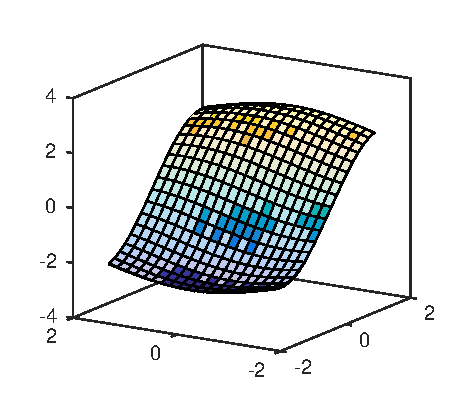
\includegraphics{plots/conclusions/robot_like_extended/phi_approx.eps}
		%\caption{$\hat{W}_\varphi(t)$}
	\end{subfigure}
	\begin{subfigure}{0.5\textwidth}
		% This file was created by matlab2tikz.
%
\definecolor{mycolor1}{rgb}{0.00000,0.44700,0.74100}%
%
\begin{tikzpicture}

\begin{axis}[%
width=0.761\textwidth,
height=0.65\textwidth,
at={(0\textwidth,0\textwidth)},
scale only axis,
xmin=-2,
xmax=2,
ymin=0.07,
ymax=0.11,
axis background/.style={fill=white},
xmajorgrids,
ymajorgrids
]
\addplot [color=red, dashed, line width=1.2pt, forget plot]
  table[row sep=crcr]{%
-1.5707963267949	0.075\\
-1.55500942903816	0.0754735872604091\\
-1.53922253128143	0.0759470564929443\\
-1.5234356335247	0.0764202896991467\\
-1.50764873576797	0.0768931689393802\\
-1.49186183801123	0.0773655763622243\\
-1.4760749402545	0.0778373942338454\\
-1.46028804249777	0.0783085049673383\\
-1.44450114474104	0.0787787911520315\\
-1.4287142469843	0.0792481355827486\\
-1.41292734922757	0.0797164212890175\\
-1.39714045147084	0.080183531564223\\
-1.38135355371411	0.0806493499946915\\
-1.36556665595737	0.0811137604887046\\
-1.34977975820064	0.0815766473054307\\
-1.33399286044391	0.0820378950837711\\
-1.31820596268717	0.0824973888711092\\
-1.30241906493044	0.0829550141519604\\
-1.28663216717371	0.0834106568765104\\
-1.27084526941698	0.0838642034890401\\
-1.25505837166024	0.0843155409562251\\
-1.23927147390351	0.0847645567953064\\
-1.22348457614678	0.0852111391021234\\
-1.20769767839005	0.0856551765790028\\
-1.19191078063331	0.0860965585624964\\
-1.17612388287658	0.0865351750509603\\
-1.16033698511985	0.0869709167319702\\
-1.14455008736312	0.087403675009564\\
-1.12876318960638	0.0878333420313063\\
-1.11297629184965	0.0882598107151674\\
-1.09718939409292	0.0886829747762105\\
-1.08140249633619	0.0891027287530801\\
-1.06561559857945	0.0895189680342852\\
-1.04982870082272	0.0899315888842705\\
-1.03404180306599	0.0903404884692698\\
-1.01825490530925	0.090745564882934\\
-1.00246800755252	0.0911467171717286\\
-0.986681109795789	0.0915438453600932\\
-0.970894212039057	0.0919368504753575\\
-0.955107314282324	0.0923256345724077\\
-0.939320416525591	0.0927101007580959\\
-0.923533518768859	0.0930901532153884\\
-0.907746621012126	0.0934656972272454\\
-0.891959723255394	0.0938366392002258\\
-0.876172825498661	0.0942028866878132\\
-0.860385927741928	0.0945643484134556\\
-0.844599029985196	0.0949209342933129\\
-0.828812132228463	0.0952725554587083\\
-0.81302523447173	0.0956191242782755\\
-0.797238336714998	0.0959605543797992\\
-0.781451438958265	0.09629676067174\\
-0.765664541201532	0.0966276593644415\\
-0.7498776434448	0.0969531679910123\\
-0.734090745688067	0.0972732054278785\\
-0.718303847931335	0.0975876919150013\\
-0.702516950174602	0.0978965490757551\\
-0.686730052417869	0.0981996999364602\\
-0.670943154661137	0.0984970689455667\\
-0.655156256904404	0.0987885819924834\\
-0.639369359147671	0.0990741664260473\\
-0.623582461390939	0.0993537510726306\\
-0.607795563634206	0.0996272662538779\\
-0.592008665877474	0.0998946438040718\\
-0.576221768120741	0.100155817087121\\
-0.560434870364008	0.100410721013169\\
-0.544647972607276	0.100659292054812\\
-0.528861074850543	0.100901468262937\\
-0.513074177093811	0.101137189282154\\
-0.497287279337078	0.101366396365844\\
-0.481500381580345	0.101589032390796\\
-0.465713483823613	0.101805041871446\\
-0.44992658606688	0.102014370973703\\
-0.434139688310147	0.102216967528364\\
-0.418352790553415	0.102412781044123\\
-0.402565892796682	0.102601762720145\\
-0.386778995039949	0.102783865458235\\
-0.370992097283217	0.102959043874573\\
-0.355205199526484	0.103127254311025\\
-0.339418301769752	0.103288454846023\\
-0.323631404013019	0.103442605305015\\
-0.307844506256286	0.103589667270475\\
-0.292057608499554	0.103729604091478\\
-0.276270710742821	0.103862380892834\\
-0.260483812986088	0.103987964583781\\
-0.244696915229356	0.10410632386623\\
-0.228910017472623	0.104217429242566\\
-0.21312311971589	0.104321253023001\\
-0.197336221959158	0.104417769332472\\
-0.181549324202425	0.104506954117091\\
-0.165762426445693	0.10458878515014\\
-0.14997552868896	0.10466324203761\\
-0.134188630932227	0.104730306223284\\
-0.118401733175495	0.10478996099336\\
-0.102614835418762	0.10484219148062\\
-0.0868279376620293	0.10488698466813\\
-0.0710410399052968	0.10492432939249\\
-0.0552541421485642	0.104954216346611\\
-0.0394672443918316	0.104976638082038\\
-0.023680346635099	0.104991589010804\\
-0.00789344887836618	0.104999065406825\\
0.0078934488783664	0.104999065406825\\
0.023680346635099	0.104991589010804\\
0.0394672443918316	0.104976638082038\\
0.0552541421485642	0.104954216346611\\
0.071041039905297	0.10492432939249\\
0.0868279376620296	0.10488698466813\\
0.102614835418762	0.10484219148062\\
0.118401733175495	0.10478996099336\\
0.134188630932227	0.104730306223284\\
0.14997552868896	0.10466324203761\\
0.165762426445693	0.10458878515014\\
0.181549324202425	0.104506954117091\\
0.197336221959158	0.104417769332472\\
0.21312311971589	0.104321253023001\\
0.228910017472623	0.104217429242566\\
0.244696915229356	0.10410632386623\\
0.260483812986088	0.103987964583781\\
0.276270710742821	0.103862380892834\\
0.292057608499554	0.103729604091478\\
0.307844506256286	0.103589667270475\\
0.323631404013019	0.103442605305015\\
0.339418301769752	0.103288454846023\\
0.355205199526484	0.103127254311025\\
0.370992097283217	0.102959043874573\\
0.386778995039949	0.102783865458235\\
0.402565892796682	0.102601762720145\\
0.418352790553415	0.102412781044123\\
0.434139688310147	0.102216967528364\\
0.44992658606688	0.102014370973703\\
0.465713483823612	0.101805041871446\\
0.481500381580345	0.101589032390796\\
0.497287279337078	0.101366396365844\\
0.51307417709381	0.101137189282154\\
0.528861074850543	0.100901468262937\\
0.544647972607275	0.100659292054812\\
0.560434870364008	0.100410721013169\\
0.576221768120741	0.100155817087121\\
0.592008665877473	0.0998946438040718\\
0.607795563634206	0.0996272662538779\\
0.623582461390939	0.0993537510726306\\
0.639369359147671	0.0990741664260473\\
0.655156256904404	0.0987885819924834\\
0.670943154661137	0.0984970689455667\\
0.686730052417869	0.0981996999364602\\
0.702516950174602	0.0978965490757551\\
0.718303847931335	0.0975876919150013\\
0.734090745688067	0.0972732054278785\\
0.7498776434448	0.0969531679910123\\
0.765664541201533	0.0966276593644415\\
0.781451438958265	0.09629676067174\\
0.797238336714998	0.0959605543797992\\
0.81302523447173	0.0956191242782755\\
0.828812132228463	0.0952725554587083\\
0.844599029985196	0.0949209342933129\\
0.860385927741928	0.0945643484134556\\
0.876172825498661	0.0942028866878132\\
0.891959723255393	0.0938366392002258\\
0.907746621012126	0.0934656972272454\\
0.923533518768859	0.0930901532153884\\
0.939320416525591	0.0927101007580959\\
0.955107314282324	0.0923256345724077\\
0.970894212039056	0.0919368504753575\\
0.986681109795789	0.0915438453600932\\
1.00246800755252	0.0911467171717287\\
1.01825490530925	0.090745564882934\\
1.03404180306599	0.0903404884692698\\
1.04982870082272	0.0899315888842705\\
1.06561559857945	0.0895189680342852\\
1.08140249633619	0.0891027287530801\\
1.09718939409292	0.0886829747762105\\
1.11297629184965	0.0882598107151674\\
1.12876318960638	0.0878333420313063\\
1.14455008736312	0.087403675009564\\
1.16033698511985	0.0869709167319702\\
1.17612388287658	0.0865351750509603\\
1.19191078063331	0.0860965585624964\\
1.20769767839005	0.0856551765790029\\
1.22348457614678	0.0852111391021234\\
1.23927147390351	0.0847645567953063\\
1.25505837166024	0.0843155409562251\\
1.27084526941698	0.0838642034890401\\
1.28663216717371	0.0834106568765104\\
1.30241906493044	0.0829550141519604\\
1.31820596268717	0.0824973888711093\\
1.33399286044391	0.0820378950837711\\
1.34977975820064	0.0815766473054308\\
1.36556665595737	0.0811137604887046\\
1.38135355371411	0.0806493499946915\\
1.39714045147084	0.080183531564223\\
1.41292734922757	0.0797164212890175\\
1.4287142469843	0.0792481355827485\\
1.44450114474104	0.0787787911520315\\
1.46028804249777	0.0783085049673383\\
1.4760749402545	0.0778373942338454\\
1.49186183801123	0.0773655763622243\\
1.50764873576797	0.0768931689393802\\
1.5234356335247	0.0764202896991467\\
1.53922253128143	0.0759470564929443\\
1.55500942903816	0.0754735872604091\\
1.5707963267949	0.075\\
};
\addplot [color=mycolor1, line width=1.2pt, forget plot]
  table[row sep=crcr]{%
-1.5707963267949	0.0727642877671847\\
-1.55500942903816	0.0735415207750309\\
-1.53922253128143	0.0742961714030801\\
-1.5234356335247	0.0750278549384516\\
-1.50764873576797	0.0757363696532353\\
-1.49186183801123	0.0764216876771912\\
-1.4760749402545	0.0770839440281161\\
-1.46028804249777	0.0777234240134606\\
-1.44450114474104	0.0783405492442384\\
-1.4287142469843	0.0789358625250333\\
-1.41292734922757	0.07951001190142\\
-1.39714045147084	0.0800637341579518\\
-1.38135355371411	0.0805978380657273\\
-1.36556665595737	0.0811131876782704\\
-1.34977975820064	0.0816106859680118\\
-1.33399286044391	0.0820912590831769\\
-1.31820596268717	0.0825558414866256\\
-1.30241906493044	0.0830053622145388\\
-1.28663216717371	0.0834407324643537\\
-1.27084526941698	0.0838628346886329\\
-1.25505837166024	0.0842725133353634\\
-1.23927147390351	0.084670567336344\\
-1.22348457614678	0.0850577444047197\\
-1.20769767839005	0.085434737161289\\
-1.19191078063331	0.0858021810678955\\
-1.17612388287658	0.0861606541059764\\
-1.16033698511985	0.0865106781000837\\
-1.14455008736312	0.0868527215508198\\
-1.12876318960638	0.0871872038099198\\
-1.11297629184965	0.0875145004029179\\
-1.09718939409292	0.08783494928254\\
-1.08140249633619	0.0881488577791909\\
-1.06561559857945	0.0884565100039932\\
-1.04982870082272	0.0887581744550225\\
-1.03404180306599	0.0890541115787312\\
-1.01825490530925	0.0893445810459955\\
-1.00246800755252	0.0896298485155296\\
-0.986681109795789	0.0899101916762258\\
-0.970894212039057	0.0901859053837993\\
-0.955107314282324	0.0904573057353307\\
-0.939320416525591	0.0907247329571753\\
-0.923533518768859	0.0909885530164442\\
-0.907746621012126	0.0912491579029697\\
-0.891959723255394	0.0915069645664239\\
-0.876172825498661	0.0917624125311183\\
-0.860385927741928	0.0920159602480147\\
-0.844599029985196	0.0922680802786996\\
-0.828812132228463	0.0925192534386418\\
-0.81302523447173	0.0927699620561312\\
-0.797238336714998	0.0930206825281873\\
-0.781451438958265	0.0932718773747754\\
-0.765664541201532	0.0935239870074123\\
-0.7498776434448	0.0937774214372786\\
-0.734090745688067	0.094032552151094\\
-0.718303847931335	0.0942897043801476\\
-0.702516950174602	0.0945491499791078\\
-0.686730052417869	0.0948111011167755\\
-0.670943154661137	0.0950757049611588\\
-0.655156256904404	0.0953430395166458\\
-0.639369359147671	0.0956131107422461\\
-0.623582461390939	0.0958858510475998\\
-0.607795563634206	0.0961611192285279\\
-0.592008665877474	0.0964387018672083\\
-0.576221768120741	0.096718316184535\\
-0.560434870364008	0.0969996142948161\\
-0.544647972607276	0.0972821887766335\\
-0.528861074850543	0.097565579439364\\
-0.513074177093811	0.0978492811334187\\
-0.497287279337078	0.0981327524245117\\
-0.481500381580345	0.0984154249289428\\
-0.465713483823613	0.0986967130885791\\
-0.44992658606688	0.0989760241514392\\
-0.434139688310147	0.0992527681168705\\
-0.418352790553415	0.0995263674034733\\
-0.402565892796682	0.099796266003214\\
-0.386778995039949	0.100061937896492\\
-0.370992097283217	0.100322894520026\\
-0.355205199526484	0.100578691101912\\
-0.339418301769752	0.10082893170554\\
-0.323631404013019	0.101073272855612\\
-0.307844506256286	0.101311425654462\\
-0.292057608499554	0.101543156334464\\
-0.276270710742821	0.101768285231534\\
-0.260483812986088	0.1019866842047\\
-0.244696915229356	0.102198272566332\\
-0.228910017472623	0.10240301162607\\
-0.21312311971589	0.102600897987633\\
-0.197336221959158	0.102791955770747\\
-0.181549324202425	0.102976227959538\\
-0.165762426445693	0.103153767103097\\
-0.14997552868896	0.103324625612996\\
-0.134188630932227	0.103488845915785\\
-0.118401733175495	0.103646450725495\\
-0.102614835418762	0.103797433701861\\
-0.0868279376620293	0.103941750754133\\
-0.0710410399052968	0.1040793122382\\
-0.0552541421485642	0.104209976276459\\
-0.0394672443918316	0.104333543405948\\
-0.023680346635099	0.104449752731108\\
-0.00789344887836618	0.104558279724011\\
0.0078934488783664	0.104658735777576\\
0.023680346635099	0.104750669577214\\
0.0394672443918316	0.10483357031437\\
0.0552541421485642	0.104906872722544\\
0.071041039905297	0.104969963873637\\
0.0868279376620296	0.105022191630854\\
0.102614835418762	0.105062874614904\\
0.118401733175495	0.105091313503804\\
0.134188630932227	0.10510680345409\\
0.14997552868896	0.105108647403437\\
0.165762426445693	0.10509616999219\\
0.181549324202425	0.105068731824805\\
0.197336221959158	0.105025743781831\\
0.21312311971589	0.104966681089339\\
0.228910017472623	0.104891096855503\\
0.244696915229356	0.104798634793389\\
0.260483812986088	0.104689040864681\\
0.276270710742821	0.104562173600618\\
0.292057608499554	0.104418012883423\\
0.307844506256286	0.104256667003211\\
0.323631404013019	0.104078377841119\\
0.339418301769752	0.103883524068255\\
0.355205199526484	0.103672622291196\\
0.370992097283217	0.103446326117079\\
0.386778995039949	0.10320542315399\\
0.402565892796682	0.102950830004162\\
0.418352790553415	0.102683585347705\\
0.434139688310147	0.102404841252032\\
0.44992658606688	0.102115852876175\\
0.465713483823612	0.101817966768893\\
0.481500381580345	0.10151260798427\\
0.497287279337078	0.101201266257807\\
0.51307417709381	0.10088548149948\\
0.528861074850543	0.100566828867581\\
0.544647972607275	0.100246903688274\\
0.560434870364008	0.0999273064807666\\
0.576221768120741	0.0996096283370366\\
0.592008665877473	0.0992954368884247\\
0.607795563634206	0.0989862630697538\\
0.623582461390939	0.0986835888654095\\
0.639369359147671	0.0983888361918586\\
0.655156256904404	0.0981033570381343\\
0.670943154661137	0.0978284249507887\\
0.686730052417869	0.0975652279136149\\
0.702516950174602	0.0973148626360247\\
0.718303847931335	0.097078330228282\\
0.734090745688067	0.0968565332077563\\
0.7498776434448	0.0966502737488419\\
0.765664541201533	0.0964602530610071\\
0.781451438958265	0.0962870717552811\\
0.797238336714998	0.0961312310399845\\
0.81302523447173	0.0959931345721256\\
0.828812132228463	0.0958730907819713\\
0.844599029985196	0.095771315485063\\
0.860385927741928	0.0956879345984294\\
0.876172825498661	0.0956229867858619\\
0.891959723255393	0.0955764258706122\\
0.907746621012126	0.0955481228723602\\
0.923533518768859	0.0955378675482745\\
0.939320416525591	0.0955453693447977\\
0.955107314282324	0.0955702576967065\\
0.970894212039056	0.0956120816422018\\
0.986681109795789	0.0956703087563775\\
1.00246800755252	0.0957443234394963\\
1.01825490530925	0.0958334246301018\\
1.03404180306599	0.0959368230451984\\
1.04982870082272	0.0960536380796223\\
1.06561559857945	0.0961828945234634\\
1.08140249633619	0.0963235192791879\\
1.09718939409292	0.0964743382782995\\
1.11297629184965	0.096634073810363\\
1.12876318960638	0.0968013424845868\\
1.14455008736312	0.096974654045592\\
1.16033698511985	0.0971524112603464\\
1.17612388287658	0.0973329110824948\\
1.19191078063331	0.0975143472836347\\
1.20769767839005	0.0976948147187387\\
1.22348457614678	0.0978723153653852\\
1.23927147390351	0.0980447662442635\\
1.25505837166024	0.0982100092922815\\
1.27084526941698	0.0983658232203013\\
1.28663216717371	0.0985099373459424\\
1.30241906493044	0.0986400473489581\\
1.31820596268717	0.0987538328533779\\
1.33399286044391	0.0988489766979278\\
1.34977975820064	0.0989231857151523\\
1.36556665595737	0.0989742128011434\\
1.38135355371411	0.0989998800227122\\
1.39714045147084	0.0989981024780589\\
1.41292734922757	0.0989669126012172\\
1.4287142469843	0.0989044845803972\\
1.44450114474104	0.0988091585463046\\
1.46028804249777	0.0986794641789226\\
1.4760749402545	0.0985141433803074\\
1.49186183801123	0.0983121716667107\\
1.50764873576797	0.0980727779457069\\
1.5234356335247	0.0977954623627006\\
1.53922253128143	0.0974800119258387\\
1.55500942903816	0.0971265136484047\\
1.5707963267949	0.0967353649825924\\
};
\end{axis}
\end{tikzpicture}%
		%\caption{$\hat{W}_\gamma(t)$)}
	\end{subfigure}
	\caption{Προσεγγίσεις των συναρτήσεων $\varphi(x)$ (αριστερά) και $\gamma(x)$ (δεξιά) στο παράδειγμα \ref{subsec:extended_grid}}
	\label{fig:robot_like_extended_approximations}
\end{figure}

\subsection{Σειρά προσπέλασης κέντρων}
\label{subsec:mixed_order}
Σε αυτό το τελευταίο πείραμα δοκιμάζουμε να τροποποιήσουμε την σειρά με την οποία η τροχιά $x(t)$ επισκέπτεται τα κέντρα του νευρωνικού δικτύου με σκοπό να εξετάσουμε τι επιπτώσεις έχει αυτό στην ποιότητα αναγνώρισης. Αρχικά σημειώνουμε πως σε όλα τα πειράματα μέχρι στιγμής, η τροχιά $x(t)$ επισκέπτεται πρώτα το κέντρο $c_\Phi$ με την μικρότερη συνιστώσα $x_1$ και την μικρότερη συνιστώσα $x_2$. Στην συνέχεια επισκέπτεται όλα τα κέντρα με το ίδιο $x_1$ αλλά μεγαλύτερα $x_2$ κατά αύξουσα σειρά, και με αυτόν τον τρόπο επισκέπτεται όλα τα κέντρα της πρώτης στήλης. Η ίδια διαδικασία επαναλαμβάνεται για κάθε επόμενη στήλη, και με αυτόν τον τρόπο η τροχιά $x(t)$ επισκέπτεται όλα τα κέντρα του νευρωνικού δικτύου. Με άλλα λόγια, στην περίπτωση ενός επίπεδου πλέγματος όπως στο Σχήμα \ref{fig:aug_phase_plain} η τροχιά επισκέπτεται τα κέντρα από κάτω προς τα πάνω και από αριστερά προς δεξιά.

Σε αυτό το πείραμα, επαυξάνουμε την τροχιά ως εξής: Κατά την πρώτη μισή περίοδο της τροχιάς επισκεπτόμαστε όλα τα κέντρα όπως περιγράψαμε στην προηγούμενη παράγραφο, και κατά την υπόλοιπη μισή επισκεπτόμαστε όλα τα κέντρα με τον αντίθετο τρόπο, δηλαδή από πάνω προς τα κάτω και από δεξιά προς αριστερά,με αποτέλεσμα η συνολική διάρκεια της περιόδου να διπλασιάζεται. Τα κέρδη και οι υπόλοιποι παράμετροι του συστήματος παραμένουν ίδια με αυτά του Πειράματος \ref{subsec:extended_grid}. Τέλος, και σε αυτή την περίπτωση θα χρησιμοποιήσουμε επαυξημένα δίκτυα RBF, όπως φαίνεται στο σχήμα \ref{fig:aug_phase_plain}.

\begin{figure}
	\begin{subfigure}{0.5\textwidth}
		% This file was created by matlab2tikz.
%
\definecolor{mycolor1}{rgb}{0.00000,0.44700,0.74100}%
\definecolor{mycolor2}{rgb}{0.85000,0.32500,0.09800}%
\definecolor{mycolor3}{rgb}{0.92900,0.69400,0.12500}%
\definecolor{mycolor4}{rgb}{0.49400,0.18400,0.55600}%
\definecolor{mycolor5}{rgb}{0.46600,0.67400,0.18800}%
%
\begin{tikzpicture}

\begin{axis}[%
width=0.761\textwidth,
height=0.65\textwidth,
at={(0\textwidth,0\textwidth)},
scale only axis,
xmin=0,
xmax=20000,
xlabel style={font=\color{white!15!black}},
xlabel={Time, $t$},
ymin=-1,
ymax=0.2,
ylabel style={font=\color{white!15!black}},
ylabel={$\hat{W}_\varphi(t)$},
axis background/.style={fill=white},
xmajorgrids,
ymajorgrids
]
\addplot [color=mycolor1, line width=1.2pt, forget plot]
  table[row sep=crcr]{%
0	0\\
4.3860770339561	0.00184611410077196\\
13.1161227931734	0.0047175857325783\\
20.0526982541669	0.00614157774907653\\
25.2700946225777	0.0111063108015514\\
30.1247001663978	0.0162652601648006\\
40.1369703611599	0.0233691076355171\\
42.7652182233905	0.0248853253469861\\
52.4063652627483	0.0354960003387532\\
57.5001659355476	0.0394813647653791\\
60.6137574353161	0.0414376866865496\\
63.2175071761194	0.0419362608372467\\
65.9762008934849	0.0440161297010491\\
71.4873369252855	0.0488675274027628\\
79.8882664389348	0.0537289516287274\\
82.2631856291482	0.0524653061183926\\
91.5508148718473	0.0550035285341437\\
98.9625618448335	0.0564044621714856\\
103.86747289732	0.0539407591240888\\
117.666264094871	0.0489793926826678\\
120.310349037463	0.0481416693910433\\
132.722080233929	0.0365366705227643\\
138.116515066955	0.0329004792292835\\
141.02215174077	0.031591283132002\\
143.810289137702	0.0291921770804038\\
148.022603235113	0.0240586296458787\\
154.651604952855	0.017673556918453\\
158.058050572348	0.0148496082838392\\
161.189210075299	0.014082458386838\\
163.748107554751	0.0125767597601225\\
167.283137061182	0.00914330944942776\\
173.78311389008	0.00410001943600946\\
177.988796876081	0.0014062493792153\\
180.972031847585	0.00101479713703156\\
184.001353612559	0.00138048775261268\\
188.492732220966	-9.74086578935385e-05\\
199.532721148677	-0.00244907373053138\\
222.014961198209	-0.00262794750597095\\
225.27908278516	-0.00408362137386575\\
236.960905847056	-0.00710568802242051\\
241.26035415359	-0.00767831020857557\\
248.751230466707	-0.00985048433358315\\
254.626647667301	-0.0103950413431448\\
258.294620156787	-0.0113724465190899\\
261.831446278135	-0.0111185509704228\\
266.023065281875	-0.0120263321441598\\
286.814384025351	-0.0125697095354553\\
306.014398137464	-0.0104566723675816\\
317.524672406435	-0.0085698176153528\\
321.341217812998	-0.0081480645458214\\
324.522827460853	-0.00694424537505256\\
330.29276380083	-0.00533086605719291\\
368.978103550187	0.00197304750690819\\
380.618429814229	0.00305335246230243\\
385.37702716389	0.00172006506545586\\
398.142246506035	0.000968708915024763\\
407.576030445707	0.000333643176418263\\
418.777111927615	-0.000958664928475628\\
423.566717324054	-0.000588448812777642\\
434.259892377875	0.000895692493941169\\
462.391884495577	0.00380843538732734\\
478.512989601768	0.0050301859373576\\
486.780927022697	0.00506856582433102\\
498.62002569258	0.00536042230305611\\
508	0.00460932508576661\\
520.012757697048	0.00424427005054895\\
524.679153016485	0.00338645291412831\\
552.933977310266	0.000474530246719951\\
558.018761734624	-0.000133780238684267\\
562	0.000138802650326397\\
566.241464748629	-0.000632603587291669\\
579.694444008936	-0.00190382664368371\\
584.009433230065	-0.000432611723226728\\
600.483028735747	-9.34239724301733e-05\\
622.34132899002	0.00172669396852143\\
637.360213849959	1.24921825772617e-05\\
645.230988815176	-0.000735137982701417\\
700.725770256351	-0.00246607784356456\\
778.435894309201	0.000898943391803186\\
783.052397528896	-0.000399478729377734\\
808.273907376206	-0.00172095904054004\\
824.217204421228	-0.00257760085150949\\
841.032811987505	-0.00103072097408585\\
900.002992089398	0.000205324908165494\\
912.020653579355	-0.000120330092613585\\
923.427553473612	-0.000668006756313844\\
978.68698151573	-0.00229007675443427\\
982.590418653232	-0.000910045066120801\\
996.630261096896	-0.000653971990686841\\
1004.04960318986	-9.23369370866567e-05\\
1020.21291217541	0.00148807644291082\\
1029.74032054675	0.000731808810087387\\
1047.3205988733	-0.000203667706955457\\
1126.17364296211	-0.0005456779654196\\
1156.47615906658	4.4448930566432e-05\\
1178.00073658047	0.000362468435923802\\
1182.60752850778	-0.000999850773951039\\
1212.09448312671	-0.00241554334570537\\
1221.92864953788	-0.00326760832103901\\
1237.55552426778	-0.00203696860262426\\
1246.96022174636	-0.00178156266338192\\
1314.35692222535	-0.00140340506914072\\
1341.85567873706	-0.00205259087670129\\
1359.56599344901	-0.00218010589742335\\
1364	-0.00196695669001201\\
1376.56552295018	-0.00236367196339415\\
1382.00413048152	-0.00105220346813439\\
1416.73024352596	0.000701845507137477\\
1422	0.0011568428708415\\
1433.7768823416	0.000209627269214252\\
1450.13940815989	-0.000226836764340987\\
1477.12711142468	-0.00053561011372949\\
1520.03624464097	-0.000602067273575813\\
1532.91926562598	-0.000370038695109542\\
1578.49038246563	-1.28290594147984e-05\\
1582.92536237267	-0.00138719400638365\\
1603.92085794064	-0.00189062340359669\\
1616.01926163052	-0.00289569099186338\\
1620.99181815326	-0.00328204789548181\\
1644.41562384955	-0.00214170057370211\\
1777.83480039047	-0.00241982841907884\\
1782	-0.00114510018465808\\
1803.6356904905	-0.000700932356267003\\
1822.00040034345	0.000756243247451494\\
1834.00196444014	-5.99141058046371e-05\\
1850.41594418812	-0.000372269540093839\\
1887.84685495281	-0.000605345838266658\\
1924.19476057393	-0.000491990664158948\\
1978.72136685298	-0.000328021837049164\\
1984.00289962102	-0.00169221992109669\\
2001.47327003141	-0.00179759348247899\\
2019.02768339683	-0.00322496184162446\\
2030.44198557626	-0.00279921154287877\\
2049.29021760895	-0.00237822203416727\\
2179.1446771959	-0.00250742804200854\\
2184.05716777642	-0.00117703283103765\\
2202.23334163976	-0.00110492399107898\\
2220.00077500619	0.00036693377114716\\
2242.34682848014	-0.000689048578351503\\
2262.66331607602	-0.000546430008398602\\
2319.99492360335	-0.000751899249735288\\
2351.56514199141	-0.000497380093293032\\
2376.00891092128	-0.000678708092891611\\
2381.34231885727	-0.00167229490034515\\
2392.27784664243	-0.00185553110713954\\
2403.02443435358	-0.00203027707902947\\
2421.39957481346	-0.00334595994354459\\
2440.00659234906	-0.00244798726271256\\
2507.61885956864	-0.00239399616111768\\
2580.88754632622	-0.00207035686617019\\
2586.00130642186	-0.00123382260062499\\
2603.20842234737	-0.00115771133278031\\
2621.50985394327	0.0001608688471606\\
2634.00132757416	-0.000492463837872492\\
2645.02453732919	-0.0007294887000171\\
2757.64039748693	-0.00067880413189414\\
2762.57972432955	-0.00102004838481662\\
2776.01788230468	-0.00087764297859394\\
2786.22931968089	-0.00205705619009677\\
2803.62413937524	-0.0020974613908038\\
2820.22070733775	-0.00322800100184395\\
2851.07752467784	-0.00254389405017719\\
2906.48773583145	-0.00247754172596615\\
2980.2917191359	-0.00255884292710107\\
2986.08285923089	-0.00129988209664589\\
3003.70895531296	-0.00130508487200132\\
3022.00028235893	-0.000133329642267199\\
3040.13291148126	-0.000955353658355307\\
3072.23992722454	-0.000929596069909167\\
3134	-0.000958065043960232\\
3177.19507303208	-0.00105606962461025\\
3182.06876359743	-0.00221207877257257\\
3204.883620413	-0.00226475464660325\\
3217.62036158901	-0.00320950851164525\\
3292.14637909454	-0.00252096157419146\\
3378.52774000273	-0.00251179915721877\\
3383.81194335413	-0.00133733010443393\\
3407.41056892955	-0.0011665186357277\\
3420.05772198268	-0.000423287816374796\\
3452.43137937325	-0.00102675493326387\\
3470.99168750315	-0.00105366039497312\\
3519.00123505063	-0.00115777554674423\\
3558.22267260872	-0.00101989657559898\\
3570.00165804687	-0.00124272097309586\\
3577.66076539808	-0.00120522982251714\\
3582.98896336087	-0.00237751441818546\\
3606.61868910828	-0.00242584299849113\\
3619.50079369701	-0.00334751880291151\\
3642.41060400993	-0.00254819836482056\\
3667.50824065465	-0.00263717857887968\\
3722.41858246729	-0.00259843357343925\\
3779.00267193491	-0.00247702599517652\\
3784	-0.00138261957545183\\
3807.21474394704	-0.00129557032050798\\
3819.80715486773	-0.000558974825253244\\
3843.63232452406	-0.00119634266229696\\
3887.77586565492	-0.00120131079165731\\
3979.44482567197	-0.00133530543826055\\
3985.25227460467	-0.00240873231814476\\
4002.94962153742	-0.00219886685590609\\
4022	-0.003220892373065\\
4039.80291345149	-0.00263405321675236\\
4180.35613468807	-0.00252670994814252\\
4186.008526929	-0.00145914577660733\\
4204.18386017828	-0.00166800784791121\\
4217.45449846659	-0.000715561985998647\\
4247.27053560331	-0.00124102179688634\\
4375.64686151576	-0.00147997543899692\\
4381.2757315542	-0.00232843536650762\\
4394	-0.00235856770450482\\
4410.31943405038	-0.00266596127767116\\
4422.47146048454	-0.0030930164102756\\
4446.14257708447	-0.00266309332437231\\
4576.84542905305	-0.00245517422808916\\
4582.51666214591	-0.00135801608848851\\
4605.6964778378	-0.00162640665803337\\
4618.43130970979	-0.000853824512887513\\
4684.66462420723	-0.00135525846781093\\
4774.82644629115	-0.00156127617447055\\
4781.26491474745	-0.00237878197367536\\
4800.01473116862	-0.00234060535876779\\
4804.19369181541	-0.00224708356836345\\
4822.34595009354	-0.00307564851027564\\
4846.33457159308	-0.00265511252655415\\
4976.48460066695	-0.00243691830110038\\
4982.01935993795	-0.00138015336415265\\
5009.11174066154	-0.00141544834696106\\
5022.12444647006	-0.000942008304264164\\
5047.15725549582	-0.00135750540721347\\
5180.74046694123	-0.00180983091922826\\
5186.38248608094	-0.00256859906221507\\
5204	-0.00222446186671732\\
5222.12237972688	-0.00307930290364311\\
5246	-0.00266074834871688\\
5380.16993728669	-0.00246787504875101\\
5386.00035926294	-0.00148371263640001\\
5404.08265250671	-0.00185542341205291\\
5418.05594286452	-0.00104725629353197\\
5466.1916232225	-0.00141328151585185\\
5550.62504929809	-0.00143022110933089\\
5576.7471512518	-0.00167063940898515\\
5582.17767979889	-0.00269146835489664\\
5606.45995683757	-0.00236277807562146\\
5619.41639144427	-0.00316174841645989\\
5638.00133541404	-0.0026881542726187\\
5694.00712010937	-0.00260432796858368\\
5759.99160254451	-0.00266734013712266\\
5798.00418609571	-0.00166606266066083\\
5803.26775520296	-0.0018844345031539\\
5822.47234476832	-0.00121455207408872\\
5855.53023396862	-0.00149581443474744\\
5958.5195095938	-0.00152219511437579\\
5969.35638836735	-0.00174329614674207\\
5976.49455743533	-0.00175088182004401\\
5982.28237382949	-0.00275666930247098\\
6005.98501995525	-0.00232446397785679\\
6018.52588162909	-0.0030590553105867\\
6056.02257515988	-0.0026687208119256\\
6157.89342963268	-0.00268893596876296\\
6169.41776932181	-0.00243984845292289\\
6176.55737722901	-0.00242849560891045\\
6182.25371069079	-0.00142317810241366\\
6205.94667501028	-0.00190963303248282\\
6218.43959768984	-0.00119055290633696\\
6256.00135005661	-0.00155223649198888\\
6317.20940352906	-0.00161595034660422\\
6377.79031670722	-0.00180168576844153\\
6383.02707349927	-0.0028434082014428\\
6405.65827632836	-0.00233143010700587\\
6422.06504058255	-0.00296632041136036\\
6444.76333580359	-0.00266703348825104\\
6580.00118726342	-0.00241576808548416\\
6585.97737689102	-0.00153440601570765\\
6610.79530611756	-0.00159781665934133\\
6623.07260171413	-0.00137673893186729\\
6666	-0.00158442139218096\\
6780.54255718903	-0.00192412823525956\\
6786.06706174131	-0.00274193783843657\\
6810	-0.00259738665408804\\
6822.00232699698	-0.00297415314707905\\
6846.00664153838	-0.00266723827007809\\
6977.92046569285	-0.00239786991005531\\
6982.93518507547	-0.0013658543866768\\
7006.46278242492	-0.00190898354412639\\
7019.1727348348	-0.00125005532390787\\
7042.52877432398	-0.00165240067872219\\
7115.46606017754	-0.00167162052093772\\
7176.51445818524	-0.00187458490836434\\
7182.25954848067	-0.00283390810727724\\
7205.67246482958	-0.00231248682393925\\
7218.30071842053	-0.00298645786824636\\
7257.12493941239	-0.00262976810699911\\
7380.0262025956	-0.00240699761343421\\
7386.01361545381	-0.00153580446567503\\
7410.98112020673	-0.00164160306303529\\
7423.60787207871	-0.00146954819501843\\
7480.61619435663	-0.00169915818332811\\
7579.54878867203	-0.0019044581495109\\
7584.9608079608	-0.00278237849852303\\
7608.33197246083	-0.00241855816784664\\
7621.28588750671	-0.00286976906500058\\
7652.07098613492	-0.00259832049050601\\
7758.2055425971	-0.00259677799476776\\
7796	-0.00166147363052005\\
7806.76852331308	-0.0018841054479708\\
7820.17198847157	-0.00139950539596612\\
7878.54905801057	-0.0016456956291222\\
7978	-0.00189107616097317\\
7983.73820586184	-0.00279473725822754\\
8006.99552290541	-0.00236724123533349\\
8019.55801394623	-0.00298510829088627\\
8032.00345927083	-0.00267252109551919\\
8117.2993636458	-0.00254014170059236\\
8175.11615797731	-0.00230122600623872\\
8186.91486869271	-0.00148111512316973\\
8205.96407429333	-0.00198625764460303\\
8218.16108822285	-0.00132087352903909\\
8248.19541419554	-0.00161834430400631\\
8380.39239240238	-0.00188395041914191\\
8386.0509529661	-0.00272163767294842\\
8410.02423359578	-0.00247287300953758\\
8422.18759039629	-0.00276034098351374\\
8453.89985984132	-0.00251543211197713\\
8554	-0.00253774408702157\\
8578.08259465595	-0.00226087472765357\\
8584.08534024982	-0.00140704939985881\\
8608	-0.00185776407306548\\
8621.37349577565	-0.00139495138864731\\
8652.00671097402	-0.00162074548279634\\
8778.07124927009	-0.00186983644380234\\
8783.61649870906	-0.0028008659974148\\
8807.43589459403	-0.00229528664567624\\
8820.1175935641	-0.00270312943030149\\
8870.70484415961	-0.00248195469248458\\
8976.19118190744	-0.00221535441232845\\
8982.18807571754	-0.00129011756871478\\
9006.52971294416	-0.00188218471521395\\
9019.48790837653	-0.00122833028581226\\
9031.4816657136	-0.00151648289102013\\
9099.73341360827	-0.00161786529133678\\
9180	-0.00186109351125197\\
9185.23499897156	-0.00269283470697701\\
9209.03422387129	-0.00235715344751952\\
9221.57350271782	-0.00266022482537664\\
9260.02242222291	-0.00243224309451762\\
9376.34290283707	-0.0021597075246973\\
9382.43191229274	-0.00122293392632855\\
9406	-0.0019345508007973\\
9419.00783661561	-0.00129643993932405\\
9442.36333764719	-0.00159114034249797\\
9556.57415368021	-0.0015713255488663\\
9593.87758091573	-0.00244843955806573\\
9610.36652298925	-0.00232968905038433\\
9622.92110843559	-0.00253657519351691\\
9737.23116825266	-0.00233249807934044\\
9776.33514921872	-0.00212076448224252\\
9782.0014750747	-0.00121796891107806\\
9812.4554832776	-0.00148752005407005\\
9824.00942689514	-0.00141161274223123\\
9906.06210295705	-0.00157319863865268\\
9980.53428516713	-0.00185421811329434\\
9986.38487458869	-0.00259316366282292\\
10011.0465932339	-0.00235983748643775\\
10017.4991322446	-0.0027206303057028\\
10028.6750193697	-0.0024590988032287\\
10177.3523249654	-0.00206746224648668\\
10184	-0.00123720342526212\\
10214.0018507736	-0.00130745155911427\\
10232.0007533442	-0.00142410113039659\\
10306	-0.00151125224147108\\
10378.0006581776	-0.00173968594390317\\
10383.8791918435	-0.00255218844176852\\
10414.090251319	-0.00247817664785543\\
10438.9504409827	-0.00234645429372904\\
10491.6272156444	-0.00223050465137931\\
10579.701230312	-0.00199374899602844\\
10586	-0.00121154655789724\\
10609.4397896563	-0.0015383786012535\\
10620.1436018561	-0.00130426660689409\\
10704.0458337842	-0.00149147103365976\\
10780.0017640709	-0.001722896231513\\
10785.9786957977	-0.0025140010729956\\
10812	-0.00232867779413937\\
10822.3380787995	-0.00241309789271327\\
10904.0067891868	-0.00220254065425252\\
10980.3843469029	-0.00194515611656243\\
10986.0104765805	-0.00116479785720003\\
11010.5672030785	-0.00149288007742143\\
11017.2221840279	-0.00113075891931658\\
11036.8512219789	-0.00137551845546113\\
11076.3477822742	-0.0014294354696176\\
11178.047493286	-0.00169794690009439\\
11184.0271556368	-0.00250217235588934\\
11208.91954586	-0.00209515583264874\\
11222.1553869496	-0.00237219413247658\\
11285.888541021	-0.00217636110028252\\
11380.0810405532	-0.00193068584849243\\
11386.1413470637	-0.00112988549881265\\
11410.9830395412	-0.00143028208185569\\
11422.5369355298	-0.00131035298545612\\
11579.375727254	-0.00166343803721247\\
11584.7201562635	-0.00248435920366319\\
11610	-0.00206708914629417\\
11622.0370756964	-0.00229786318959668\\
11673.6994861147	-0.00212768715573475\\
11775.1394348042	-0.00186424811181496\\
11781.7665551791	-0.000983825611911016\\
11806.0070444479	-0.00172005838976474\\
11818.7618067971	-0.00110726308412268\\
11838	-0.00130916556008742\\
11906.2780310472	-0.00139009138001711\\
11978.5603955618	-0.00161551019118633\\
11984.5840671347	-0.00242978029564256\\
12009.83474021	-0.00201334718076396\\
12022.0032512911	-0.00224509556574048\\
12098.2073224506	-0.00204007933643879\\
12180.0122583529	-0.00180677007665508\\
12186.0003154268	-0.00102594810232404\\
12210.0020699868	-0.00140848629598622\\
12216.0013352284	-0.00106405126280151\\
12254.0024572046	-0.00133655124227516\\
12380.0268570499	-0.00158730455950717\\
12386.0517595239	-0.00236015689733904\\
12409.5587766901	-0.00196385582603398\\
12422.0029944167	-0.00219088223093422\\
12504.3793651264	-0.00199468405116932\\
12578.3959563461	-0.00177249185435358\\
12584.014990335	-0.000969746310147457\\
12614.9576460152	-0.00113698241693783\\
12778.2524286	-0.00154410530012683\\
12783.9870142814	-0.0023335664300248\\
12813.6377962283	-0.00217377359149395\\
12832	-0.00207730779220583\\
12976.8746690194	-0.00172606906926376\\
12982.7019020688	-0.000786082015110878\\
13007.8802994775	-0.00151340628872276\\
13020.2606303773	-0.00114852320257341\\
13105.7357612538	-0.00130313615954947\\
13180.0396456094	-0.00152318894106429\\
13186.0012615461	-0.00228559443712584\\
13209.553812567	-0.00188685399189126\\
13222.1908536106	-0.00210309482645243\\
13310.00967779	-0.00192078546024277\\
13380.0022938202	-0.00166970562349888\\
13385.7285998105	-0.000905781053006649\\
13410.016876023	-0.00132215733174235\\
13422.5071958338	-0.00113178658648394\\
13574.5511244528	-0.00148598021041835\\
13581.1768971429	-0.00213976614031708\\
13594.0788878841	-0.0020189666756778\\
13612	-0.00198053391795838\\
13623.106811347	-0.00201644607659546\\
13780.2778396426	-0.00165875392121961\\
13786.3720878766	-0.00088890624101623\\
13812.0044034427	-0.0011509221221786\\
13823.4276075854	-0.00113079246148118\\
13980.3730961934	-0.0014694516066811\\
13986.5637281419	-0.00222803231372382\\
14005.1933547352	-0.00161824931637966\\
14017.0251187681	-0.00211911763472017\\
14045.9434957413	-0.00189797584243934\\
14134.1398159071	-0.00180093219751143\\
14179.7284190758	-0.00160475059237797\\
14185.0891781118	-0.000824332368210889\\
14209.512574717	-0.00125195029613678\\
14222	-0.0010475526942173\\
14273.321068672	-0.00116334338963497\\
14378.4730485635	-0.00143155196565203\\
14384.0043844292	-0.00221254918142222\\
14414	-0.00203675747616217\\
14442.3913980585	-0.00189575654439977\\
14698.1021633533	-0.00118182017831714\\
14778.6812109406	-0.00140949072738294\\
14784.2384850745	-0.00218983746162849\\
14808.0646068203	-0.00158522067067679\\
14815.5112920462	-0.00207824321478256\\
14844.5401741531	-0.00186562414091895\\
14912.3092435058	-0.00179258379648672\\
14974.9555139683	-0.00154909341654275\\
14981.8140437645	-0.000682450718159089\\
15012.9807090556	-0.00105255433300044\\
15024.0721807918	-0.00103493678761879\\
15177.4655815902	-0.00137425012508174\\
15183.4957444613	-0.00229137277347036\\
15206.9064564171	-0.00156727739522466\\
15219.9833587925	-0.0018959418302984\\
15313.4451159289	-0.00174903652805369\\
15376.3287397141	-0.00150563413990312\\
15382.9544387774	-0.000568243165616877\\
15406.3820218856	-0.00138923494523624\\
15420	-0.000976299339527031\\
15477.9352881036	-0.00106974359368905\\
15576.1189626807	-0.00136190044213436\\
15581.8332432918	-0.0022057313217374\\
15612.003968832	-0.00182058495556703\\
15623.4337834625	-0.00182722687895875\\
15778.2487109337	-0.0014711241965415\\
15784.0316075796	-0.00069282563708839\\
15824.960616322	-0.000977748946752399\\
15976.006455983	-0.00132764456793666\\
15981.5590141018	-0.00217361214890843\\
16012	-0.00177448711110628\\
16022.3046573191	-0.00182191140265786\\
16176.6826330767	-0.00141579541377723\\
16182.6019482985	-0.000499105859489646\\
16205.5729975761	-0.00131580626111827\\
16218.0180727121	-0.000777926623413805\\
16241.860637681	-0.000980167205852922\\
16377.1528508642	-0.00126825007828302\\
16383.1131098186	-0.00219435217150021\\
16407.3584408123	-0.00146736914757639\\
16419.4099721174	-0.00196760128164897\\
16430.2788831961	-0.00175252468034159\\
16577.6180875857	-0.0013862313098798\\
16583.4044262424	-0.000457758782431483\\
16605.7447871598	-0.00129432991161593\\
16618.1252892291	-0.000745061461202567\\
16642.2387715827	-0.000954256644035922\\
16778.4190446052	-0.00123286106463638\\
16784.1552976129	-0.00200013672656496\\
16820.052736928	-0.00172070816188352\\
16902.1062104793	-0.00155070347318542\\
16974.9328347484	-0.00131802710166085\\
16981.2487950943	-0.000586849171668291\\
16999.4654260428	-0.000898076916200807\\
17004.0202242691	-0.00125654071962344\\
17022.15232319	-0.000795176183601143\\
17138.8955259667	-0.000984291851636954\\
17176.0180377098	-0.00119917268602876\\
17181.835864005	-0.00202520069433376\\
17212.1851582871	-0.00162839472250198\\
17217.4349325036	-0.001880961972347\\
17228.5018823774	-0.0016401966495323\\
17378.9414247396	-0.00127464093384333\\
17384.6779741668	-0.000483208074001595\\
17408.0780971908	-0.00112078167148866\\
17415.3213718133	-0.000651773614663398\\
17451.6969902492	-0.000878089183970587\\
17580.187243945	-0.00113074039472849\\
17586.1955819958	-0.00189262190906447\\
17610.0138069799	-0.00143332461084356\\
17622.3291208503	-0.00163595888807322\\
17780.4171863904	-0.00121028638386633\\
17786.5067956851	-0.000481490915262839\\
17810.418046564	-0.000916390199563466\\
17822	-0.00072569161420688\\
17882.2368927853	-0.000822354915726464\\
17980.0020571975	-0.00110509648584411\\
17986.0003595712	-0.00186045166265103\\
18010.2176157006	-0.00140243975329213\\
18016.1731898298	-0.0017382954392815\\
18045.0198968463	-0.00153414768283255\\
18104.9728433045	-0.00143566777478554\\
18179.9515608367	-0.00119307944260072\\
18185.7584257167	-0.000446415200713091\\
18208.1173292807	-0.001043051815941\\
18215.3287186661	-0.000578814102482283\\
18244.6034135547	-0.000774854677729309\\
18349.1214336051	-0.000840259584947489\\
18374.6210987157	-0.00108313507735147\\
18380.4285943608	-0.00110291815144592\\
18386.014254642	-0.0018357590015512\\
18410.0002086335	-0.0013599075791717\\
18421.843683368	-0.00156553729539155\\
18483.0258425715	-0.0014412650889426\\
18580.0026376039	-0.00115027271021972\\
18586.0003136327	-0.000404170848923968\\
18608.2034789208	-0.000987246996373869\\
18615.4899191259	-0.000507639557326911\\
18638.8858599441	-0.000688796731992625\\
18705.4056079213	-0.000777538389229449\\
18774.3373038273	-0.0010055483362521\\
18780.0671586662	-0.000997801336779958\\
18786.0709294446	-0.00175297205714742\\
18810.4651853817	-0.00129982859652955\\
18822.4953367927	-0.00145562256147969\\
18967.932758524	-0.00117862109982525\\
18975.804953639	-0.00108911586357863\\
18982.0083986769	-0.000229052420763765\\
19010.1664430106	-0.000800645506387809\\
19022.1615463142	-0.000603937922278419\\
19138.4685027893	-0.000764066866395297\\
19176.9552389569	-0.000973022673861124\\
19182.4426285041	-0.00185650620551314\\
19206.0090281809	-0.00101862284282106\\
19219.0904940867	-0.00158407300841645\\
19231.0924208811	-0.00143195183773059\\
19360.0017687439	-0.00132609563297592\\
19398	-0.000512801758304704\\
19403.3560536935	-0.000942843304073904\\
19444.4772171971	-0.000617324898485094\\
19550.0837433423	-0.000660550547763705\\
19577.4443070689	-0.000904587828699732\\
19583.0372549935	-0.00182952308750828\\
19606.023132065	-0.000944046671065735\\
19618.3515198795	-0.00149863147453289\\
19637.1652074935	-0.00134773761965334\\
19690.5729067539	-0.00124077189320815\\
19776.8223401651	-0.000986287883279147\\
19783.0968390723	-5.95183482801076e-05\\
19806.6769198332	-0.000855556987517048\\
19819.1004419028	-0.00036434398862184\\
19837.630172438	-0.000553139791009016\\
19978.0070245124	-0.000861252992763184\\
19984.0031967615	-0.00162377288506832\\
19997.4360428969	-0.00137447392262402\\
};
\addplot [color=mycolor2, line width=1.2pt, forget plot]
  table[row sep=crcr]{%
0	0\\
161.189210075299	5.16592990607023e-09\\
163.748107554751	-0.0124172903088038\\
167.283137061182	-0.0232914547850669\\
173.78311389008	-0.0232914547850669\\
177.988796876081	-0.0271345200308133\\
180.972031847585	-0.0402473048961838\\
184.001353612559	-0.0617598709723097\\
188.492732220966	-0.0791865776955092\\
195.713248301421	-0.079792455315328\\
199.532721148677	-0.115338011190033\\
202.551419989839	-0.134805934099859\\
206.476039022979	-0.154333107097045\\
213.576425201514	-0.154333107097045\\
218.01797911034	-0.168167911429919\\
222.014961198209	-0.18494243305031\\
225.27908278516	-0.211000463117671\\
232.001842891772	-0.210975451234845\\
236.960905847056	-0.211506032497709\\
241.26035415359	-0.23438705530134\\
558.018761734624	-0.23438705530134\\
566.241464748629	-0.242903895006748\\
574.076152414127	-0.242903895006748\\
579.694444008936	-0.248678932748589\\
584.009433230065	-0.256771389016649\\
590.061411881768	-0.261929370335565\\
596.201135599451	-0.262056180617947\\
600.483028735747	-0.275108642767009\\
604.353202437225	-0.287632490024407\\
608.002447958523	-0.288356362023478\\
614.470020621637	-0.288359084785043\\
622.34132899002	-0.302826507268037\\
626.472081648732	-0.314377283986687\\
637.360213849959	-0.314571721279208\\
640.960872313997	-0.32560529053444\\
960	-0.32560529053444\\
963.297048149354	-0.329740176293853\\
967.544653650682	-0.331086075846542\\
978.68698151573	-0.33142959574252\\
982.590418653232	-0.334439137946902\\
986.499758192516	-0.337979654366791\\
996.630261096896	-0.338013506159768\\
1000.23794635831	-0.343594351703359\\
1004.04960318986	-0.347684945543733\\
1009.2893710913	-0.347253604180878\\
1016.23989025102	-0.347401621122117\\
1020.21291217541	-0.355034693493508\\
1024.15339099646	-0.361157251099939\\
1029.74032054675	-0.361999926666613\\
1036.12838047548	-0.362068977367016\\
1041.53291943875	-0.368179762775981\\
1359.56599344901	-0.368179762775981\\
1364	-0.372265381593024\\
1382.00413048152	-0.372063262922893\\
1386.01498284864	-0.374188029669313\\
1398.03381819099	-0.374464791850187\\
1400.96049507244	-0.37883139454425\\
1404.05736239145	-0.377918004134699\\
1410.00043795923	-0.377066173714411\\
1416.73024352596	-0.376935548818437\\
1422	-0.383195025224268\\
1426.02427942527	-0.387011576218356\\
1433.7768823416	-0.387011576218356\\
1438.73605921448	-0.388065096474747\\
1443.98863234149	-0.39088757285208\\
1760.93630678806	-0.39088757285208\\
1765.65415039241	-0.394434281362919\\
1777.83480039047	-0.394466781352094\\
1782	-0.393711091608566\\
1794.31065211661	-0.393900378556282\\
1799.56877257293	-0.395197362169711\\
1808.85404353281	-0.393058716377709\\
1816.26257895748	-0.392800924844778\\
1822.00040034345	-0.397828587923868\\
1826.42280624487	-0.400278552555392\\
1834.00196444014	-0.400278552555392\\
1839.14190882368	-0.400744865179149\\
1844	-0.40284698704636\\
2161.05045522956	-0.40284698704636\\
2165.82149543082	-0.405868027668475\\
2184.05716777642	-0.405794029815297\\
2191.56787093688	-0.40483178741124\\
2198	-0.404655280570296\\
2202.23334163976	-0.405879216683388\\
2207.92338712808	-0.402124946598633\\
2214.70855618389	-0.40211795131836\\
2220.00077500619	-0.404752814203675\\
2225.00822174687	-0.407777813059511\\
2237.68337523915	-0.407922734513704\\
2242.34682848014	-0.409381487759674\\
2557.87843467179	-0.409381487759674\\
2562.36302384057	-0.412172922719037\\
2580.88754632622	-0.411538358624966\\
2586.00130642186	-0.410445766679914\\
2598.4244963844	-0.410196094351704\\
2603.20842234737	-0.409871164589276\\
2608.30837067618	-0.408158031816129\\
2616.00203663573	-0.408176353626914\\
2621.50985394327	-0.411583752378647\\
2626.6826365949	-0.412691217821703\\
2634.00132757416	-0.412691217821703\\
2640	-0.413546128518647\\
2957.9415912792	-0.413546128518647\\
2963.35271485713	-0.415976238811709\\
2980.2917191359	-0.415085521333822\\
2986.08285923089	-0.413727020950319\\
2998.46858316225	-0.413427156305261\\
3003.70895531296	-0.411760099519597\\
3009.79883518193	-0.41043531179821\\
3016.21670832729	-0.410057209122897\\
3022.00028235893	-0.413975199582637\\
3027.68706158989	-0.414760561383446\\
3359.96449512314	-0.415042969114438\\
3364.42348980069	-0.417051357468154\\
3378.52774000273	-0.417083822678251\\
3383.81194335413	-0.415818980491167\\
3390.02314330782	-0.415109879882948\\
3402.00070083009	-0.41551848439849\\
3407.41056892955	-0.41194666786032\\
3414.14354831608	-0.411940089790733\\
3420.05772198268	-0.414735069967719\\
3426.04321613051	-0.415841289479431\\
3760.25349406547	-0.415711318382819\\
3765.87893814197	-0.4176948029708\\
3772.00844598166	-0.4176948029708\\
3779.00267193491	-0.417121402420889\\
3784	-0.417259447425749\\
3790.01362921075	-0.415699667784793\\
3802	-0.415429524226056\\
3807.21474394704	-0.411825157316343\\
3814.32318713087	-0.411817711137701\\
3819.80715486773	-0.412665475516405\\
3824.55786815104	-0.415181041531469\\
3830.96085873412	-0.41526097869064\\
3838	-0.414782099654985\\
3850.04945701887	-0.415056588681182\\
4156	-0.415056588681182\\
4161.60729824319	-0.415742338176642\\
4166.78747155507	-0.417106718919968\\
4174.42079892056	-0.417106718989089\\
4180.35613468807	-0.416518152760545\\
4186.008526929	-0.415355085508054\\
4199.69920908746	-0.415015606900852\\
4204.18386017828	-0.413464307246613\\
4210.01672148872	-0.412277060859196\\
4217.45449846659	-0.41181144228176\\
4222.64887150725	-0.415719441669353\\
4236.00036768463	-0.415694701605389\\
4241.68880411974	-0.415138102984201\\
4558.02683919401	-0.415138102984201\\
4563.21316326852	-0.417196888425678\\
4576.84542905305	-0.416854929368128\\
4582.51666214591	-0.415324253237486\\
4595.66885797214	-0.415366666140471\\
4600.13194876381	-0.416051665946725\\
4605.6964778378	-0.413417173676862\\
4612.06735615634	-0.413404005881603\\
4618.43130970979	-0.41264886908175\\
4624.00143909062	-0.416324275331135\\
4637.0459217206	-0.416403010694921\\
4642.2038884471	-0.415493938671716\\
4958.29018426899	-0.415493938671716\\
4963.47160791572	-0.417653246706323\\
4968.62019323589	-0.417273452188965\\
4976.48460066695	-0.41727496155363\\
4986.89115325239	-0.415399172663456\\
4998.77442477505	-0.41560064602163\\
5003.74518269702	-0.413935900200158\\
5009.11174066154	-0.412632684368873\\
5016.25538165978	-0.412148404924665\\
5022.12444647006	-0.415596449427539\\
5047.15725549582	-0.414595412668859\\
5357.86970157766	-0.414595412668859\\
5362.39532228047	-0.416275576553744\\
5367.69805186419	-0.415873793594074\\
5375.01633467082	-0.415876689050492\\
5380.16993728669	-0.415334465713386\\
5386.00035926294	-0.414222674353368\\
5393.33322183941	-0.414222674353368\\
5404.08265250671	-0.412916857538221\\
5411.17945273413	-0.411715630500112\\
5418.05594286452	-0.411675479506812\\
5423.68138400583	-0.41475567593443\\
5436.12388088367	-0.414963977909792\\
5441.40629968047	-0.413801441391115\\
5759.99160254451	-0.413801441391115\\
5765.79644472312	-0.41540437248841\\
5778.45357870185	-0.41546216370989\\
5784.79342048958	-0.413936961107538\\
5798.00418609571	-0.413400817222282\\
5816.34425736445	-0.411044320517249\\
5822.47234476832	-0.414623084740015\\
5828.26639588486	-0.414080558937712\\
5835.9281415041	-0.414080558937712\\
5841.69816286223	-0.412885078410909\\
6157.89342963268	-0.412885078410909\\
6163.40113289037	-0.414772199073923\\
6176.55737722901	-0.414434856709704\\
6182.25371069079	-0.412885304041993\\
6200.58026212779	-0.412352954459493\\
6205.94667501028	-0.41062807038179\\
6212.35146997302	-0.410628052071843\\
6218.43959768984	-0.410004546502023\\
6224.11246875417	-0.413311567317578\\
6237.55665622546	-0.413332701446052\\
6243.11691098119	-0.411874668046948\\
6556.00105726413	-0.411874668046948\\
6561.74714998187	-0.413180387582543\\
6604.06217201273	-0.410653290404298\\
6610.79530611756	-0.409437983871612\\
6617.88310480663	-0.410020103030547\\
6623.07260171413	-0.411560568565619\\
6636.18955774061	-0.411596162244678\\
6641.63638612618	-0.410152823380486\\
6958.44693703752	-0.410152823380486\\
6963.76866407636	-0.411540946981404\\
6977.92046569285	-0.411348313587951\\
6982.93518507547	-0.409977780524059\\
7001.06570148909	-0.410675318435096\\
7006.46278242492	-0.408191822756635\\
7019.1727348348	-0.40775576136366\\
7024.63547247626	-0.410602626740001\\
7031.7271020044	-0.410560337440984\\
7048.57879611459	-0.409082392023265\\
7356	-0.409082392023265\\
7362	-0.410788846482319\\
7380.0262025956	-0.410122129997035\\
7386.01361545381	-0.4091272957412\\
7399.90650256244	-0.408835632548289\\
7404.52075655431	-0.40863849127345\\
7410.98112020673	-0.40749217407938\\
7417.92488821408	-0.408071726789785\\
7423.60787207871	-0.409935966363264\\
7437.10767466227	-0.409973739100678\\
7442.00339735004	-0.408520589393447\\
7758.2055425971	-0.408520589393447\\
7763.83568499504	-0.410233337493992\\
7776.4397716401	-0.410058964967902\\
7782.50992905337	-0.408855871384731\\
7801.6551815576	-0.409767832250509\\
7806.76852331308	-0.407201294448896\\
7814.05658748212	-0.407198008328123\\
7820.17198847157	-0.410380575616728\\
7826	-0.409695169659244\\
7833.4089579781	-0.409695169659244\\
7839.36158962216	-0.409133723467676\\
7844.7942195516	-0.408067760396079\\
8156.22014229914	-0.408067760396079\\
8162.63617280085	-0.409437823662302\\
8168.00207151662	-0.409082332345861\\
8175.11615797731	-0.409086576171831\\
8218.16108822285	-0.405883049483236\\
8223.69172880752	-0.408756954293494\\
8236.4502259316	-0.408747698405932\\
8242.02494030242	-0.407137179397978\\
8559.90157237587	-0.407137179397978\\
8564.9963670772	-0.408622782491875\\
8578.08259465595	-0.408678403477097\\
8584.08534024982	-0.407674905203748\\
8596.39409329918	-0.407604244061076\\
8602.00160370192	-0.408289540959231\\
8608	-0.406011686463899\\
8615.23648944945	-0.406007266064989\\
8621.37349577565	-0.408945768500416\\
8626.63192382595	-0.408315091655822\\
8639.6282182539	-0.407892673276365\\
8644.32393098653	-0.406754903895489\\
8958	-0.406754903895489\\
8963.12715485966	-0.408392700723198\\
8968.7302970186	-0.408021307332092\\
8976.19118190744	-0.408024554108124\\
8982.18807571754	-0.407037791748735\\
8996	-0.407081107281556\\
9001.01666776223	-0.408217991327547\\
9006.52971294416	-0.406042541573697\\
9019.48790837653	-0.405759134384425\\
9024.16588726926	-0.407566142093856\\
9037.70594905195	-0.407521967714274\\
9042.4394518377	-0.405951540007663\\
9357.55689405854	-0.405951540007663\\
9362.64903792512	-0.40760861353192\\
9376.34290283707	-0.407360243971198\\
9382.43191229274	-0.40612953740856\\
9394.55758428752	-0.406485609179072\\
9419.00783661561	-0.405152168576024\\
9424.2373243132	-0.407599905975076\\
9437.73159389608	-0.407504173192137\\
9442.36333764719	-0.405739565569093\\
9757.19776766968	-0.405739565569093\\
9762.94733636724	-0.406953573950886\\
9800.34441838639	-0.405469878834992\\
9806.09366451535	-0.404557585468865\\
9818.37654781268	-0.404274729266035\\
9824.00942689514	-0.406357963685878\\
9837.64800304041	-0.406319295252615\\
9842.32543159498	-0.404381687370915\\
10158.1006625411	-0.404381687370915\\
10164.0076272487	-0.405480212451948\\
10184	-0.405564717129892\\
10190	-0.404671604497707\\
10196.1765902808	-0.404646992967173\\
10201.9634100511	-0.40553383498991\\
10207.4745871735	-0.403618311858736\\
10219.0338121878	-0.403307232591033\\
10224.6026948023	-0.405759599183511\\
10237.4166069196	-0.405708475092979\\
10242.96775977	-0.403811100630264\\
10556.0488012701	-0.403811100630264\\
10562.0490512106	-0.405381803622731\\
10567.1672204955	-0.404940495296614\\
10579.701230312	-0.40467138461463\\
10586	-0.403970357216167\\
10592.7080814661	-0.403970357216167\\
10598.6476551469	-0.403485782200733\\
10604.0049495513	-0.404330408346141\\
10609.4397896563	-0.403220321808476\\
10615.3309328601	-0.403216565580806\\
10620.1436018561	-0.405551848514733\\
10625.8202735072	-0.404710789396631\\
10632.5112676773	-0.404710757669818\\
10638.2474154467	-0.404246281468659\\
10644.0176724043	-0.402903328431421\\
10961.25549636	-0.402903295616852\\
10966.3768478056	-0.404094373672706\\
10980.3843469029	-0.403861493490695\\
10986.0104765805	-0.403238373612112\\
11004.4367356805	-0.403464450162573\\
11010.5672030785	-0.402374319521186\\
11017.2221840279	-0.401878892123932\\
11023.1353777563	-0.404473326991138\\
11036.8512219789	-0.404581709553895\\
11042.0049089472	-0.40258758339769\\
11360.8861117854	-0.40258758339769\\
11366.4158689369	-0.403624755730561\\
11380.0810405532	-0.403449163826735\\
11386.1413470637	-0.402745618073823\\
11399.2782192509	-0.402550233888178\\
11404.5080097551	-0.403267814173887\\
11410.9830395412	-0.402115618380776\\
11417.0946033547	-0.401613263475156\\
11422.5369355298	-0.405175347543263\\
11428.3022394094	-0.404140572394681\\
11436.0096229558	-0.404143423133064\\
11441.0703315444	-0.402252739397227\\
11756.2858462238	-0.402252739397227\\
11762.481817975	-0.403849697901023\\
11775.1394348042	-0.403568314675795\\
11781.7665551791	-0.403330545988865\\
11786.9681470944	-0.402390510815167\\
11800.306053966	-0.402145804378961\\
11806.0070444479	-0.401773228393722\\
11818.7618067971	-0.401566434040433\\
11824.5220371746	-0.403805726127757\\
11838	-0.403249020368094\\
11842.8250405969	-0.402028054697439\\
12161.0988323106	-0.402028054682887\\
12166.0181114001	-0.403088850522181\\
12180.0122583529	-0.402770326432801\\
12186.0003154268	-0.402044758004195\\
12192.7410567668	-0.402044758004195\\
12198.219882698	-0.401428371595102\\
12203.9307241881	-0.402636363643978\\
12210.0020699868	-0.401515616318648\\
12216.0013352284	-0.401239799295581\\
12222	-0.404455463081831\\
12227.4493595412	-0.403397705635143\\
12235.0592922925	-0.403397705635143\\
12240.0769302046	-0.401579362376651\\
12560.2155245644	-0.401579362376651\\
12565.2783081285	-0.402666080179188\\
12584.014990335	-0.402580261103139\\
12590	-0.401772414963489\\
12596.6531241689	-0.401749438133265\\
12602.2301279471	-0.402687438294379\\
12608	-0.401082398198923\\
12614.9576460152	-0.401078111957759\\
12620.1303494792	-0.403763891888957\\
12626	-0.402811535583169\\
12632.8665091014	-0.402811535583169\\
12639.2394207026	-0.402352243236237\\
12644.488475232	-0.400998684599472\\
12958.6541210734	-0.400998684599472\\
12963.7073245694	-0.402265710585198\\
12976.8746690194	-0.402169467175554\\
12982.7019020688	-0.401090541196027\\
12988.7187445753	-0.401574699251796\\
12996.1950506378	-0.401553321182291\\
13002.0010326417	-0.402600787710981\\
13007.8802994775	-0.401046092800243\\
13014.7893275398	-0.401041866734886\\
13020.2606303773	-0.404048485186649\\
13025.7183648266	-0.403621206438402\\
13038.6181865948	-0.403182279209432\\
13043.7942621503	-0.40173518231677\\
13361.0357136545	-0.40173518231677\\
13366.0093597685	-0.402843998042954\\
13380.0022938202	-0.402558970479731\\
13398.0726760531	-0.401548489924608\\
13403.9290038312	-0.404246338304802\\
13410.016876023	-0.403078637405997\\
13417.0985262698	-0.402559060483327\\
13422.5071958338	-0.405958760911744\\
13428.4074272697	-0.404838092472346\\
13436.0012411683	-0.404838424230547\\
13441.0156645599	-0.402748895281547\\
13761.0037351478	-0.402748895281547\\
13766.4582300541	-0.403794112171454\\
13780.2778396426	-0.403551460880408\\
13786.3720878766	-0.402962691972789\\
13799.4888847755	-0.402612824829703\\
13804.5946116094	-0.403423607749573\\
13812.0044034427	-0.40227339239209\\
13818	-0.402453476046503\\
13823.4276075854	-0.405033252751309\\
13835.8418330717	-0.404906790230598\\
13840.6663147411	-0.402865263684362\\
14159.9193722037	-0.402865263684362\\
14165.5993428606	-0.403947961105587\\
14179.7284190758	-0.403684426953987\\
14198.0120734977	-0.402384823781176\\
14203.4709224361	-0.403342936177069\\
14209.512574717	-0.402213656816457\\
14216.0027177873	-0.401914260964986\\
14222	-0.404939581880171\\
14226.9966590845	-0.403964612942218\\
14234.5062887166	-0.403964612942218\\
14240.0803596094	-0.402047597570345\\
14561.2747393859	-0.40204756296589\\
14566.1105366485	-0.402943099295953\\
14579.9784826181	-0.402750018889492\\
14598.2498899121	-0.401567541022814\\
14604	-0.402615777773462\\
14610.35984555	-0.401479507268959\\
14617.6044118584	-0.400916203634551\\
14622.8361865046	-0.403995808457694\\
14628.5458535029	-0.403392819938745\\
14635.8723748681	-0.403392819938745\\
14641.0508773101	-0.401450200581166\\
14956.5786787176	-0.401450200581166\\
14962.0788930926	-0.402770412983955\\
14974.9555139683	-0.40244320642887\\
14994.8793802012	-0.401990123340511\\
15012.9807090556	-0.401356416045019\\
15018.5812082704	-0.40137990815856\\
15024.0721807918	-0.404227831710159\\
15030.8780725801	-0.404086537182593\\
15038	-0.403456855190598\\
15042.5673795628	-0.40198174715988\\
15356.9388617535	-0.40198174715988\\
15362.7440342856	-0.403348667114187\\
15396	-0.402383586981159\\
15401.1600303664	-0.403036341405823\\
15406.3820218856	-0.401907554383797\\
15414.0012061089	-0.401907479172223\\
15420	-0.404885952921177\\
15424.7274108026	-0.404287034125446\\
15438.5058147024	-0.403576392018294\\
15444.0043338073	-0.402039424065151\\
15759.5138066326	-0.402039424065151\\
15764.567871621	-0.403205120248458\\
15784.0316075796	-0.402935877438722\\
15790.1635087758	-0.402402267143771\\
15796.4988897659	-0.40238127010889\\
15802	-0.403412601663149\\
15806.9431118451	-0.401975395539921\\
15813.7509374078	-0.401975395539921\\
15819.9936267808	-0.404784051381284\\
15824.960616322	-0.403809962102969\\
15832.5260855055	-0.403861004971986\\
15838.8165446752	-0.403372984743328\\
15844.002068608	-0.401865351359447\\
16158.1387475848	-0.401865351359447\\
16163.3328331693	-0.403266167446418\\
16205.5729975761	-0.401693150692154\\
16218.0180727121	-0.401760486296553\\
16223.75037817	-0.403723063533107\\
16236.0568648659	-0.403600927918887\\
16241.860637681	-0.401516190904658\\
16558.4597718643	-0.401516190904658\\
16564.0032746372	-0.402498335923156\\
16577.6180875857	-0.402549304384593\\
16583.4044262424	-0.401597526997648\\
16595.5577552082	-0.401758930162032\\
16605.7447871598	-0.401384388158476\\
16618.1252892291	-0.401262296782079\\
16624.0003300288	-0.403434221367206\\
16637.2745142647	-0.403315750991169\\
16642.2387715827	-0.401298084943846\\
16956.0135646714	-0.401298084943846\\
16962.1083408632	-0.402646847767755\\
16974.9328347484	-0.402356310958567\\
16993.8049828248	-0.401794812707521\\
16999.4654260428	-0.402299972145556\\
17004.0202242691	-0.403312022819591\\
17010.0659138712	-0.402142905808432\\
17016.3748948419	-0.401617775052728\\
17022.15232319	-0.405178306788002\\
17028.0037237492	-0.403974162458326\\
17035.2551461017	-0.403974162458326\\
17040.51332241	-0.401975013279298\\
17359.6242560375	-0.401975013279298\\
17365.044414288	-0.403038411146554\\
17378.9414247396	-0.40273590765355\\
17398	-0.401580252819258\\
17402.6732049963	-0.404000970251218\\
17408.0780971908	-0.402562758230488\\
17415.3213718133	-0.402559436697629\\
17421.5546420545	-0.405487760101096\\
17426.254609041	-0.404505212631193\\
17434.0136724613	-0.404505212631193\\
17439.4653129961	-0.403947164199053\\
17444.0776614461	-0.402455908253614\\
17761.1766980291	-0.402455907460535\\
17766.9232985776	-0.403440383965062\\
17780.4171863904	-0.403238569615496\\
17786.5067956851	-0.402712617455109\\
17799.7067648884	-0.403098016846343\\
17804.0535003981	-0.403946019683644\\
17810.418046564	-0.402829799160827\\
17816.7025463774	-0.402341969100235\\
17822	-0.405426113000431\\
17827.3584218074	-0.404216538452602\\
17839.5444412216	-0.403775357248378\\
17844.1753674243	-0.402284165455058\\
18160.7598839476	-0.402284165455058\\
18166.0015323343	-0.403399621707649\\
18185.7584257167	-0.403112335112382\\
18198.000475606	-0.402278007786663\\
18202.2782632167	-0.403870962214569\\
18208.1173292807	-0.402484072634252\\
18215.3287186661	-0.402481222441565\\
18220.6996425685	-0.405677401900903\\
18226.2701469205	-0.404615131119499\\
18234.2461520239	-0.404615131119499\\
18240.0001511085	-0.402528335078387\\
18556.5046527763	-0.402528335078387\\
18561.9757022142	-0.403815112415032\\
18566.6201148672	-0.403436808413971\\
18580.0026376039	-0.403157292250398\\
18598	-0.402290449423162\\
18602.7519963828	-0.404069823645841\\
18608.2034789208	-0.402415650361945\\
18615.4899191259	-0.402412340725277\\
18620.8028195018	-0.405539872197551\\
18626.0616486635	-0.404424535856378\\
18634	-0.404424535856378\\
18638.8858599441	-0.403855342232418\\
18644.0016276096	-0.402277114873868\\
18956.6476568813	-0.402277114873868\\
18962.4013278519	-0.403591864316695\\
18987.8401344687	-0.402685718618159\\
19010.1664430106	-0.402358050218027\\
19016.7282114301	-0.401895690250967\\
19022.1615463142	-0.404945243211841\\
19027.826633325	-0.403878601839097\\
19034.6164581855	-0.403878601839097\\
19040.0045883689	-0.40186571823142\\
19360.0017687439	-0.40186571823142\\
19366	-0.402840952010592\\
19385.4729149138	-0.402435191903351\\
19398	-0.401630756379745\\
19403.3560536935	-0.402739062454202\\
19408.3314020993	-0.401733312137367\\
19415.4484783927	-0.40172960023483\\
19421.1397085571	-0.404594095278298\\
19426.4155243961	-0.403534670069348\\
19434.0235486297	-0.403534670069348\\
19439.7342663401	-0.402871825670445\\
19444.4772171971	-0.401547986090009\\
19758.0038591424	-0.401547986090009\\
19763.3451571389	-0.402826802936033\\
19788.7392190578	-0.40200353628461\\
19796.0013994515	-0.401980963561073\\
19801.3561092718	-0.403932122215338\\
19806.6769198332	-0.402523628014023\\
19819.1004419028	-0.402557511697523\\
19824.2938170482	-0.404745949857897\\
19837.630172438	-0.404646344581124\\
19842.5415227002	-0.402440778332675\\
19997.4360428969	-0.402440778332675\\
};
\addplot [color=mycolor3, line width=1.2pt, forget plot]
  table[row sep=crcr]{%
0	0\\
154.651604952855	0\\
158.058050572348	-0.0018833400317817\\
161.189210075299	-0.033991901880654\\
173.78311389008	-0.0339918782774475\\
177.988796876081	-0.037474935004866\\
180.972031847585	-0.0565844714583363\\
199.532721148677	-0.056952337425173\\
202.551419989839	-0.0647037114176783\\
218.01797911034	-0.0647934909356991\\
222.014961198209	-0.0834353555146663\\
225.27908278516	-0.100198474247009\\
236.960905847056	-0.100266506928165\\
241.26035415359	-0.104358308202791\\
244.319758355301	-0.121387631596008\\
552.933977310266	-0.121387631596008\\
558.018761734624	-0.121930030920339\\
562	-0.144656929554912\\
574.076152414127	-0.144656966302136\\
579.694444008936	-0.147125689229142\\
584.009433230065	-0.157972689044982\\
596.201135599451	-0.1579694069369\\
600.483028735747	-0.161047901616257\\
604.353202437225	-0.163284836224193\\
618.306723326896	-0.163284836224193\\
622.34132899002	-0.185457545110694\\
626.472081648732	-0.187901232537115\\
637.360213849959	-0.187901232537115\\
640.960872313997	-0.189959177245328\\
645.230988815176	-0.200707201955083\\
954.626128634405	-0.200707201955083\\
960	-0.202802039388189\\
963.297048149354	-0.218517021232401\\
974.319634438485	-0.21851705062727\\
978.68698151573	-0.219849422941479\\
982.590418653232	-0.228344436411135\\
996.630261096896	-0.228341872410965\\
1000.23794635831	-0.230295741675945\\
1004.04960318986	-0.23169261275325\\
1020.21291217541	-0.23169261275325\\
1024.15339099646	-0.250177482645086\\
1036.12838047548	-0.250241457721131\\
1041.53291943875	-0.251423266669008\\
1047.3205988733	-0.259172252139251\\
1359.56599344901	-0.259384116758156\\
1364	-0.27347638610081\\
1376.56552295018	-0.273488995731896\\
1382.00413048152	-0.280820546573523\\
1398.03381819099	-0.280711314193468\\
1404.05736239145	-0.283344493163895\\
1416.73024352596	-0.283344493163895\\
1422	-0.291542818948074\\
1426.02427942527	-0.298648007137672\\
1438.73605921448	-0.298647638526745\\
1443.98863234149	-0.304861382974195\\
1756	-0.304869893130672\\
1760.93630678806	-0.317186249314545\\
1777.83480039047	-0.317193921546277\\
1782	-0.32298422963504\\
1799.56877257293	-0.322847630781325\\
1803.6356904905	-0.324960853511584\\
1816.26257895748	-0.324844426744676\\
1822.00040034345	-0.331693259857275\\
1826.42280624487	-0.337597782148805\\
1839.14190882368	-0.338045675853209\\
1844	-0.34214149116815\\
2156.12014866959	-0.342140968787135\\
2161.05045522956	-0.352224975638819\\
2179.1446771959	-0.352394728499348\\
2184.05716777642	-0.356979488355137\\
2198	-0.356916081789677\\
2202.23334163976	-0.358560711891187\\
2220.00077500619	-0.358459247723658\\
2225.00822174687	-0.369068262531073\\
2237.68337523915	-0.369071306799015\\
2242.34682848014	-0.372461261478747\\
2538.9269814029	-0.372451273007755\\
2557.87843467179	-0.372446783811029\\
2562.36302384057	-0.380794223645353\\
2575.75306862592	-0.380794252869237\\
2580.88754632622	-0.385101061539899\\
2598.4244963844	-0.385025492319983\\
2603.20842234737	-0.386556849571207\\
2621.50985394327	-0.386478323638585\\
2626.6826365949	-0.395645053835324\\
2640	-0.395822007962124\\
2645.02453732919	-0.398385573767882\\
2957.9415912792	-0.398366934103251\\
2963.35271485713	-0.40574778240989\\
2975.18035308678	-0.405747787401197\\
2980.2917191359	-0.409137541882956\\
2998.46858316225	-0.409066107313265\\
3003.70895531296	-0.410547473045881\\
3016.21670832729	-0.410494540305081\\
3027.68706158989	-0.418431406949821\\
3040.13291148126	-0.418512867250683\\
3045.75964155029	-0.420568878540507\\
3359.96449512314	-0.420701666447712\\
3364.42348980069	-0.427234790509829\\
3378.52774000273	-0.427253746147471\\
3383.81194335413	-0.430257223451918\\
3396.84907946357	-0.430257065519982\\
3402.00070083009	-0.431552586273028\\
3420.05772198268	-0.431596538386657\\
3426.04321613051	-0.438562754130544\\
3440	-0.438579118748748\\
3445.17427079158	-0.440351725417713\\
3755.45297203302	-0.440351725417713\\
3760.25349406547	-0.445318236816092\\
3765.87893814197	-0.446379125551175\\
3779.00267193491	-0.446189925496583\\
3784	-0.448843580339599\\
3797.05338104771	-0.448843512218446\\
3802	-0.45008756488096\\
3819.80715486773	-0.4501126182804\\
3824.55786815104	-0.456340594755602\\
3838	-0.456339257896616\\
3843.63232452406	-0.457820461066149\\
3912.49075603126	-0.457775379763916\\
4156	-0.457775379763916\\
4161.60729824319	-0.463094587350497\\
4174.42079892056	-0.463094656101021\\
4180.35613468807	-0.465198951103957\\
4199.69920908746	-0.465199870886863\\
4204.18386017828	-0.466395496772748\\
4217.45449846659	-0.466395496772748\\
4222.64887150725	-0.47168671909094\\
4241.68880411974	-0.471476346643612\\
4247.27053560331	-0.472758055890154\\
4558.02683919401	-0.472688285655749\\
4563.21316326852	-0.4771971067712\\
4576.84542905305	-0.477201058456558\\
4582.51666214591	-0.478950949061982\\
4595.66885797214	-0.478950949061982\\
4605.6964778378	-0.480238741653011\\
4618.43130970979	-0.480238741653011\\
4624.00143909062	-0.48491709676091\\
4637.0459217206	-0.484871884964377\\
4642.2038884471	-0.486087491834041\\
4661.11096810897	-0.48592382746574\\
4958.29018426899	-0.485780290022376\\
4963.47160791572	-0.490115856773627\\
4976.48460066695	-0.490118650566728\\
4982.01935993795	-0.491483004676411\\
4998.77442477505	-0.491519746534323\\
5003.74518269702	-0.4927783117746\\
5016.25538165978	-0.492822214007901\\
5022.12444647006	-0.497144620625477\\
5065.88666080884	-0.498101032899285\\
5357.86970157766	-0.498100405606237\\
5362.39532228047	-0.501864997586381\\
5375.01633467082	-0.501865000132966\\
5380.16993728669	-0.503164631922118\\
5399.25352695007	-0.503191774430888\\
5404.08265250671	-0.504461169322894\\
5418.05594286452	-0.504461169322894\\
5423.68138400583	-0.508545368913474\\
5429.66264508495	-0.507992634768016\\
5441.40629968047	-0.507924410121632\\
5446.69732057735	-0.508764439717197\\
5759.99160254451	-0.508935467496485\\
5765.79644472312	-0.512144068779889\\
5778.45357870185	-0.511911434867216\\
5784.79342048958	-0.513278146165248\\
5798.00418609571	-0.513342341513635\\
5803.26775520296	-0.51445419096126\\
5816.34425736445	-0.514526448023389\\
5822.47234476832	-0.51841975944626\\
5903.61078151424	-0.519159359078913\\
6157.89342963268	-0.519157236281899\\
6163.40113289037	-0.522504131695314\\
6176.55737722901	-0.522506493311084\\
6182.25371069079	-0.523741369899653\\
6195.93530275005	-0.523741369899653\\
6205.94667501028	-0.524966561548354\\
6218.43959768984	-0.524966561548354\\
6224.11246875417	-0.527998766770907\\
6237.55665622546	-0.528048103296896\\
6243.11691098119	-0.528603834987734\\
6328.47378811541	-0.528573953997693\\
6556.00105726413	-0.528573961648362\\
6561.74714998187	-0.53158386987343\\
6573.58236654385	-0.531583871317707\\
6580.00118726342	-0.532413515647931\\
6599.19693324724	-0.532483123675775\\
6604.06217201273	-0.533801043176936\\
6617.88310480663	-0.533801043176936\\
6623.07260171413	-0.537009010517068\\
6641.63638612618	-0.536742332235008\\
6647.91660965886	-0.537241426707624\\
6958.44693703752	-0.537114028822543\\
6963.76866407636	-0.53986926235666\\
6977.92046569285	-0.539790843904484\\
6982.93518507547	-0.540556244028267\\
6995.71569278754	-0.540556244028267\\
7006.46278242492	-0.542020570945169\\
7019.1727348348	-0.542020570945169\\
7024.63547247626	-0.544679257105599\\
7356	-0.545103642412869\\
7362	-0.547765650710062\\
7374.09655438909	-0.547765649225767\\
7380.0262025956	-0.548470968460606\\
7399.90650256244	-0.548743846826255\\
7404.52075655431	-0.549799704931502\\
7417.92488821408	-0.549799704931502\\
7423.60787207871	-0.552343568135257\\
7437.10767466227	-0.552122784876701\\
7447.18216597752	-0.552467323443125\\
7758.2055425971	-0.552365517076396\\
7763.83568499504	-0.554976017312583\\
7776.4397716401	-0.55497632681363\\
7788.05475457277	-0.55543873005081\\
7796	-0.55543873005081\\
7806.76852331308	-0.556920873055788\\
7820.17198847157	-0.556920873055788\\
7826	-0.5589177840302\\
8156.22014229914	-0.559104378793563\\
8162.63617280085	-0.561538365982415\\
8194.20625102684	-0.561916270333313\\
8205.96407429333	-0.563460704368481\\
8218.16108822285	-0.563460704368481\\
8223.69172880752	-0.565467254833493\\
8236.4502259316	-0.565233967106906\\
8242.02494030242	-0.565708605456166\\
8255.70238906601	-0.565483794594911\\
8559.90157237587	-0.565428011595941\\
8564.9963670772	-0.567410992836813\\
8596.39409329918	-0.567631077348778\\
8602.00160370192	-0.569055588624906\\
8621.37349577565	-0.569138834634941\\
8626.63192382595	-0.570867818634724\\
8958	-0.570764533335023\\
8963.12715485966	-0.572528768963821\\
8996	-0.572815553419787\\
9006.52971294416	-0.574425153183256\\
9019.48790837653	-0.574425153183256\\
9024.16588726926	-0.576092478295323\\
9357.55689405854	-0.576215185155888\\
9362.64903792512	-0.578058829312795\\
9394.55758428752	-0.578038014966296\\
9412.91881080002	-0.579475766593532\\
9419.00783661561	-0.579475766593532\\
9424.2373243132	-0.581018261844292\\
9757.19776766968	-0.581041200061009\\
9762.94733636724	-0.582862108123663\\
9794.68424285803	-0.582732035949448\\
9806.09366451535	-0.584194006911275\\
9818.37654781268	-0.584194006911275\\
9824.00942689514	-0.585600460362912\\
9882.00695799139	-0.585556792164425\\
10158.1006625411	-0.585506658884697\\
10164.0076272487	-0.587124111454614\\
10177.3523249654	-0.587123616864119\\
10184	-0.587638745269942\\
10196.1765902808	-0.587638830620563\\
10201.9634100511	-0.588853935591032\\
10219.0338121878	-0.588723130524158\\
10224.6026948023	-0.590300174877484\\
10556.0488012701	-0.590352691826411\\
10562.0490512106	-0.591719563770312\\
10598.6476551469	-0.591861646335019\\
10604.0049495513	-0.593189842609718\\
10620.1436018561	-0.593189842609718\\
10625.8202735072	-0.593735383652529\\
10954.6339697305	-0.593769807674107\\
10961.25549636	-0.595132051355904\\
10998.9709024616	-0.595264010116807\\
11004.4367356805	-0.596619220534194\\
11017.2221840279	-0.596619220534194\\
11023.1353777563	-0.598193636280484\\
11036.8512219789	-0.597966726021696\\
11048.2074303253	-0.598231343097723\\
11354.7588450888	-0.598231343097723\\
11360.8861117854	-0.599327975891356\\
11399.2782192509	-0.599319209431997\\
11404.5080097551	-0.600836949881341\\
11417.0946033547	-0.600836949881341\\
11422.5369355298	-0.601862405565043\\
11436.0096229558	-0.601615695813962\\
11464.5167616013	-0.601562809744792\\
11756.2858462238	-0.601563185253326\\
11762.481817975	-0.60271030927106\\
11800.306053966	-0.603057475098467\\
11806.0070444479	-0.603876429951924\\
11818.7618067971	-0.603876429951924\\
11824.5220371746	-0.60488431749036\\
12154.9814010346	-0.604785046896723\\
12161.0988323106	-0.606000163727003\\
12198.219882698	-0.605969425880176\\
12203.9307241881	-0.607194767449982\\
12216.0013352284	-0.607257626823412\\
12227.4493595412	-0.608238441924186\\
12554	-0.608071791612019\\
12560.2155245644	-0.609028428618331\\
12572.1806410049	-0.609120803514088\\
12584.014990335	-0.608879813091335\\
12596.6531241689	-0.608880103249248\\
12602.2301279471	-0.610100701029296\\
12639.2394207026	-0.611137380805303\\
12778.2524286	-0.611119615965436\\
12958.6541210734	-0.611087350738671\\
12963.7073245694	-0.612139277363895\\
12996.1950506378	-0.612021871747856\\
13002.0010326417	-0.613219693284918\\
13056.9628613483	-0.613838631619728\\
13354.5760413214	-0.613838631619728\\
13361.0357136545	-0.614964060736384\\
13398.0726760531	-0.614880147488293\\
13403.9290038312	-0.616118429388735\\
13460.0238794057	-0.616290162084624\\
13754.5766007657	-0.616290162084624\\
13761.0037351478	-0.617261985898949\\
13799.4888847755	-0.617109947605059\\
13804.5946116094	-0.61836894577209\\
13818	-0.61836894577209\\
13823.4276075854	-0.619192007492529\\
13840.6663147411	-0.618896048883471\\
13880.0989291939	-0.618831355481234\\
14159.9193722037	-0.618830305127631\\
14165.5993428606	-0.619754521150753\\
14198.0120734977	-0.619659649524692\\
14203.4709224361	-0.620907524757058\\
14240.0803596094	-0.621613872703165\\
14265.6249698658	-0.62150086622205\\
14555.1543138067	-0.62150086622205\\
14561.2747393859	-0.622115301899612\\
14598.2498899121	-0.622158893485903\\
14604	-0.623548673946061\\
14617.6044118584	-0.623548673946061\\
14622.8361865046	-0.624098334825248\\
14654.3584586951	-0.62383958636201\\
14956.5786787176	-0.623839836047409\\
14962.0788930926	-0.624722677021055\\
15000.3790249013	-0.625147769482282\\
15006.0004182459	-0.626069382207788\\
15356.9388617535	-0.626128451709519\\
15362.7440342856	-0.626590708710864\\
15376.3287397141	-0.626587992210261\\
15388.4474662547	-0.626120601733419\\
15396	-0.626120601733419\\
15406.3820218856	-0.627719964784774\\
15420	-0.627719964784774\\
15424.7274108026	-0.628177281796525\\
15759.5138066326	-0.628032526266907\\
15764.567871621	-0.628632333489804\\
15796.4988897659	-0.628263755588705\\
15802	-0.629653293373849\\
15838.8165446752	-0.63027576951572\\
15850.6671493895	-0.630077001751488\\
16194.6278845038	-0.630188502818783\\
16212.3374537589	-0.631660388455202\\
16558.4597718643	-0.631697715925839\\
16564.0032746372	-0.632234905744554\\
16600.6315930503	-0.632455501105142\\
16605.7447871598	-0.633462656947813\\
16618.1252892291	-0.633462656947813\\
16624.0003300288	-0.634017448581289\\
16721.7518470101	-0.633658875220135\\
16999.4654260428	-0.633693093383044\\
17004.0202242691	-0.635211755092314\\
17016.3748948419	-0.635211755092314\\
17022.15232319	-0.635691637959098\\
17035.2551461017	-0.635417049856187\\
17124.5135861474	-0.635181904661295\\
17398	-0.635422971481603\\
17402.6732049963	-0.636415548291552\\
17415.3213718133	-0.636625426439423\\
17754.2348094241	-0.636803813744336\\
17766.9232985776	-0.63709924307841\\
17799.7067648884	-0.636877860499226\\
17804.0535003981	-0.638288092039147\\
18198.000475606	-0.638288575501065\\
18202.2782632167	-0.639583766434953\\
18220.6996425685	-0.639773245562537\\
18244.6034135547	-0.639697768649057\\
18556.5046527763	-0.639697839120345\\
18566.6201148672	-0.640188588866295\\
18574.0147686112	-0.640188588633464\\
18580.0026376039	-0.639644845068688\\
18598	-0.639842238237179\\
18602.7519963828	-0.640990095875168\\
18615.4899191259	-0.641189157136978\\
18995.0704980144	-0.641053985593317\\
19010.1664430106	-0.642707102440909\\
19398	-0.642770563586964\\
19403.3560536935	-0.643974857739522\\
19415.4484783927	-0.644201521532523\\
19801.3561092718	-0.644077338507486\\
19806.6769198332	-0.645008303374198\\
19997.4360428969	-0.644997847015475\\
};
\addplot [color=mycolor4, line width=1.2pt, forget plot]
  table[row sep=crcr]{%
0	0\\
120.310349037463	-0\\
122.540857019998	-0.0184350557537982\\
132.722080233929	-0.0184350557537982\\
138.116515066955	-0.020462197233428\\
141.02215174077	-0.0204026056453586\\
143.810289137702	-0.0314631491783075\\
148.022603235113	-0.0832561666211404\\
154.651604952855	-0.187402804127487\\
158.058050572348	-0.201928084712563\\
161.189210075299	-0.201900153508177\\
163.748107554751	-0.206103062158945\\
167.283137061182	-0.241417520970572\\
173.78311389008	-0.587631674778095\\
177.988796876081	-0.630731032946642\\
180.972031847585	-0.630731038378144\\
184.001353612559	-0.635033911985374\\
188.492732220966	-0.668100756975036\\
195.713248301421	-0.729649269298534\\
199.532721148677	-0.729821101795096\\
202.551419989839	-0.725472113597789\\
206.476039022979	-0.722083319138619\\
213.576425201514	-0.723867073680594\\
218.01797911034	-0.723842537299788\\
222.014961198209	-0.719670820140891\\
225.27908278516	-0.720521264032868\\
232.001842891772	-0.805370873742504\\
236.960905847056	-0.832454916046117\\
241.26035415359	-0.83066268053517\\
244.319758355301	-0.833169292283856\\
254.626647667301	-0.868599804674886\\
258.294620156787	-0.869986637761031\\
261.831446278135	-0.866745808343694\\
266.023065281875	-0.866114022002876\\
278.553179509818	-0.866113570573361\\
282.509898529053	-0.862385163662111\\
520.012757697048	-0.862385163662111\\
524.679153016485	-0.853593213538261\\
537.69156808035	-0.853315362452122\\
541.681807515935	-0.851499630229227\\
546.005998293218	-0.842571564739046\\
552.933977310266	-0.847338685285649\\
558.018761734624	-0.844777309048368\\
562	-0.844721394816588\\
566.241464748629	-0.843094731204474\\
574.076152414127	-0.875209323123272\\
579.694444008936	-0.876458838589315\\
590.061411881768	-0.87126772321426\\
596.201135599451	-0.871938855234475\\
600.483028735747	-0.865374400029395\\
604.353202437225	-0.857175205353997\\
608.002447958523	-0.852234953857987\\
614.470020621637	-0.845750903892622\\
618.306723326896	-0.842809990594105\\
622.34132899002	-0.839082134771161\\
626.472081648732	-0.83689842153035\\
632.111122475464	-0.872396297669184\\
637.360213849959	-0.880301052049617\\
640.960872313997	-0.879023918740131\\
645.230988815176	-0.879556525869702\\
650.576309553293	-0.883867396416463\\
656.220174566119	-0.887361531425995\\
660.327945793091	-0.883721288693778\\
664.800060107395	-0.883350779327884\\
678.137935653929	-0.88335918557641\\
683.266333443116	-0.881132674552646\\
918.104048398058	-0.881132674552646\\
923.427553473612	-0.877172789954784\\
937.541167768912	-0.877051281924651\\
941.574518528731	-0.876128710224293\\
946.673954130787	-0.869880882393772\\
954.626128634405	-0.869654860664014\\
960	-0.868179320128547\\
963.297048149354	-0.867931536049582\\
967.544653650682	-0.868833636359341\\
974.319634438485	-0.884827535646764\\
978.68698151573	-0.885440400845255\\
986.499758192516	-0.881289565350016\\
992.547311098886	-0.882431452384481\\
996.630261096896	-0.882500241496018\\
1000.23794635831	-0.877946030999738\\
1004.04960318986	-0.872121087653795\\
1009.2893710913	-0.866468793745298\\
1016.23989025102	-0.861759947321843\\
1020.21291217541	-0.856966236326116\\
1024.15339099646	-0.855659282355191\\
1029.74032054675	-0.870537395821884\\
1036.12838047548	-0.891676811501384\\
1041.53291943875	-0.890258504699887\\
1047.3205988733	-0.889762725186301\\
1054.15973905802	-0.892190916940308\\
1059.46179942569	-0.88992012480594\\
1064.00661483677	-0.888780915087409\\
1076.683400597	-0.888968293173093\\
1080.58778234222	-0.887638202420931\\
1319.89734401457	-0.887638202420931\\
1324.00982171523	-0.885731844718975\\
1341.85567873706	-0.885278910234774\\
1346.28511861751	-0.881047924362065\\
1353.68369788399	-0.880922585092776\\
1359.56599344901	-0.879285063820134\\
1364	-0.879674593739765\\
1369.51977565794	-0.883892523172108\\
1376.56552295018	-0.89202075709909\\
1382.00413048152	-0.891868471520866\\
1386.01498284864	-0.888834725075867\\
1393.43965138225	-0.890474953997909\\
1398.03381819099	-0.888474493916874\\
1400.96049507244	-0.88652237115457\\
1404.05736239145	-0.882476675560611\\
1410.00043795923	-0.876344455420622\\
1416.73024352596	-0.871135878012865\\
1422	-0.868938587067532\\
1426.02427942527	-0.868922364490572\\
1433.7768823416	-0.895637033674575\\
1438.73605921448	-0.897425910403399\\
1443.98863234149	-0.897524505850015\\
1457.87421311871	-0.893951421294332\\
1462.81302598067	-0.893353363771894\\
1477.12711142468	-0.893548474217823\\
1482.8939926497	-0.892712091823341\\
1717.91811122773	-0.892712091823341\\
1723.02469285336	-0.891962386456726\\
1742	-0.891806666269986\\
1748.03172957832	-0.887934582762682\\
1756	-0.887704810113064\\
1760.93630678806	-0.886641467313893\\
1765.65415039241	-0.887967596325325\\
1771.95725863461	-0.892960364613828\\
1777.83480039047	-0.89575352693646\\
1782	-0.895753437951498\\
1787.70823049469	-0.892709045787342\\
1794.31065211661	-0.894808742730675\\
1799.56877257293	-0.891757865152613\\
1816.26257895748	-0.879460015643417\\
1822.00040034345	-0.876730234442221\\
1826.42280624487	-0.87727576994439\\
1834.00196444014	-0.899545071653847\\
1839.14190882368	-0.901185585040366\\
1844	-0.901036973766168\\
1850.41594418812	-0.898849441011407\\
1857.20562410212	-0.897821935304819\\
1862.59078699778	-0.89616990963259\\
1876.27204885009	-0.896374160398409\\
1882.04484484951	-0.895710754666652\\
2117.96812027134	-0.895710754666652\\
2123.21991697565	-0.895225230564392\\
2142.02556353378	-0.895221601283993\\
2148.25602959186	-0.891752520987211\\
2156.12014866959	-0.891535567865503\\
2161.05045522956	-0.890690427469963\\
2165.82149543082	-0.892332476232696\\
2172.46640810795	-0.895456685037061\\
2179.1446771959	-0.897576347600989\\
2184.05716777642	-0.896114442952239\\
2191.56787093688	-0.896407440442999\\
2198	-0.895854587481153\\
2202.23334163976	-0.893617754773004\\
2207.92338712808	-0.889602470804675\\
2214.70855618389	-0.884119274156546\\
2220.00077500619	-0.881708874239848\\
2225.00822174687	-0.882690347105381\\
2231.77270223702	-0.897321360134811\\
2237.68337523915	-0.903766062034265\\
2242.34682848014	-0.903686719851976\\
2248.72781267489	-0.900412775376026\\
2256.51589885541	-0.899547806937335\\
2262.66331607602	-0.898229806138261\\
2277.50932422192	-0.89849433913696\\
2282.88246931895	-0.897806874596426\\
2519.67999745417	-0.897806874596426\\
2524.75973829261	-0.897252128896071\\
2538.9269814029	-0.897302320179733\\
2544	-0.895645703283662\\
2550.68787482423	-0.894289010575449\\
2557.87843467179	-0.893391503344901\\
2562.36302384057	-0.893353144077992\\
2568.00245026534	-0.895518695033388\\
2575.75306862592	-0.897887133352924\\
2580.88754632622	-0.898475677717215\\
2586.00130642186	-0.896486239878868\\
2592.70089853193	-0.898111563456041\\
2598.4244963844	-0.897766100566514\\
2603.20842234737	-0.896179006376769\\
2608.30837067618	-0.892965303741221\\
2616.00203663573	-0.887477001710067\\
2621.50985394327	-0.885726353226346\\
2626.6826365949	-0.887848633334215\\
2634.00132757416	-0.903244528206415\\
2640	-0.905127981801343\\
2645.02453732919	-0.902916291295696\\
2652.12372631207	-0.901925573307381\\
2659.21521784256	-0.899407526379946\\
2664.0580802943	-0.899021876255574\\
2678.18121112781	-0.899219675622589\\
2683.94516292382	-0.898758292492857\\
2919.53480739363	-0.898758292492857\\
2924.15923964415	-0.898290032455407\\
2943.37907015351	-0.898395606989652\\
2949.54455226547	-0.895636298944737\\
2963.35271485713	-0.894722046374227\\
2968.25726669767	-0.897149874024763\\
2975.18035308678	-0.89859281646568\\
2980.2917191359	-0.899181860215322\\
2986.08285923089	-0.897307157927571\\
2993.29942792438	-0.899555583677284\\
2998.46858316225	-0.899201127096603\\
3003.70895531296	-0.897189885945409\\
3009.79883518193	-0.893284069828951\\
3016.21670832729	-0.890138208327699\\
3022.00028235893	-0.888904020554037\\
3027.68706158989	-0.892224023089511\\
3034.79057268119	-0.904799078380165\\
3040.13291148126	-0.906421894062078\\
3045.75964155029	-0.90409399937198\\
3052.68647003	-0.903231218642759\\
3059.21351851228	-0.900806104433286\\
3236.49779252613	-0.900385508750333\\
3340.91007277853	-0.900141351830825\\
3346.58771511979	-0.897908814080438\\
3354.12704319752	-0.897868271455081\\
3359.96449512314	-0.897090567199484\\
3372.01441860973	-0.898825994943763\\
3378.52774000273	-0.900158525251754\\
3383.81194335413	-0.898925147619593\\
3390.02314330782	-0.898920119139802\\
3396.84907946357	-0.901292367725546\\
3402.00070083009	-0.899458572323056\\
3407.41056892955	-0.898280678800802\\
3414.14354831608	-0.893071903938107\\
3420.05772198268	-0.891916907101404\\
3426.04321613051	-0.892548327294207\\
3434.00714386817	-0.905610189678555\\
3440	-0.90750572703837\\
3445.17427079158	-0.905329611661728\\
3452.43137937325	-0.904546087182098\\
3459.42285803045	-0.902141846545419\\
3470.99168750315	-0.902073292960267\\
3717.68355145342	-0.901764401576656\\
3722.41858246729	-0.90122104178954\\
3742.00007825748	-0.901320030523493\\
3747.96793012279	-0.899079459122731\\
3755.45297203302	-0.899248380839708\\
3760.25349406547	-0.898604995963979\\
3765.87893814197	-0.899662211373652\\
3772.00844598166	-0.899672116200236\\
3779.00267193491	-0.900739344568137\\
3784	-0.899506363857654\\
3790.01362921075	-0.899965912874904\\
3797.05338104771	-0.902611754565442\\
3802	-0.900643421726272\\
3807.21474394704	-0.900122511440713\\
3814.32318713087	-0.894732898104849\\
3819.80715486773	-0.894248983320722\\
3824.55786815104	-0.894597153899667\\
3830.96085873412	-0.902203871562961\\
3838	-0.908467092096544\\
3843.63232452406	-0.907708775957872\\
3850.04945701887	-0.905502133809932\\
3858.00434945116	-0.903560280621605\\
3863.89793248815	-0.903211550117703\\
3876.81198285445	-0.903414404114301\\
3887.77586565492	-0.903142050527094\\
4118.52064449089	-0.903142050527094\\
4123.74188665722	-0.902516187928995\\
4142.03477404663	-0.902665050201904\\
4148.0429879058	-0.900546197553922\\
4156	-0.900902286957717\\
4161.60729824319	-0.900340622843942\\
4166.78747155507	-0.901064833033161\\
4180.35613468807	-0.901928183819109\\
4186.008526929	-0.900212125819962\\
4193.19243321094	-0.90347175082934\\
4204.18386017828	-0.902589415090915\\
4210.01672148872	-0.900108875641308\\
4217.45449846659	-0.897495735494886\\
4222.64887150725	-0.897319418832922\\
4228.03371453363	-0.899255858133984\\
4236.00036768463	-0.909225605420943\\
4241.68880411974	-0.909732739979518\\
4247.27053560331	-0.906867087222054\\
4254.44302420264	-0.906766576568771\\
4260.38408599086	-0.904710500486544\\
4273.67182822577	-0.904972307314893\\
4292.10788858409	-0.904746181811788\\
4538.99137707689	-0.904409530125122\\
4544.03537714469	-0.903561664130393\\
4563.21316326852	-0.902818056903925\\
4569.17593396928	-0.903975077450013\\
4576.84542905305	-0.903776353079593\\
4582.51666214591	-0.902531952513527\\
4588	-0.902100592833449\\
4595.66885797214	-0.905994666893093\\
4600.13194876381	-0.904613788366987\\
4605.6964778378	-0.904733563256741\\
4612.06735615634	-0.900251402286813\\
4624.00143909062	-0.899700771562493\\
4630.03478874417	-0.90523457186282\\
4637.0459217206	-0.910958939221018\\
4642.2038884471	-0.911536148960295\\
4648.00100463447	-0.908868125927256\\
4656.00233289408	-0.908172596980876\\
4661.11096810897	-0.90692324061456\\
4674.06767605479	-0.907156559209398\\
4684.66462420723	-0.906958611834852\\
4939.05953594959	-0.906634487470001\\
4944.00027369042	-0.905876688309945\\
4963.47160791572	-0.905102943033853\\
4968.62019323589	-0.906186002634058\\
4976.48460066695	-0.905445592252363\\
4982.01935993795	-0.905425194407144\\
4986.89115325239	-0.903918673859152\\
4993.23877745275	-0.907588010522886\\
5003.74518269702	-0.907384054000431\\
5009.11174066154	-0.906511909288383\\
5016.25538165978	-0.903464664337662\\
5022.12444647006	-0.903209291656822\\
5028.08887359138	-0.905397093978536\\
5036	-0.913162900971656\\
5041.95371818855	-0.913157085942657\\
5047.15725549582	-0.910647383556352\\
5055.22133685163	-0.910523679242033\\
5060.40283803836	-0.908631733891525\\
5073.61762980129	-0.908913581475645\\
5092.01276973582	-0.908748294292309\\
5338.57976211988	-0.908397951960069\\
5343.70490877033	-0.907547291535593\\
5362.39532228047	-0.906775424915395\\
5367.69805186419	-0.907481629343238\\
5375.01633467082	-0.906276881069061\\
5380.16993728669	-0.906378881456476\\
5386.00035926294	-0.904500040582207\\
5393.33322183941	-0.909007591857517\\
5404.08265250671	-0.908603557039896\\
5411.17945273413	-0.905998116177216\\
5423.68138400583	-0.904983055064804\\
5429.66264508495	-0.909596932389832\\
5436.12388088367	-0.913949440182478\\
5441.40629968047	-0.914434836606233\\
5446.69732057735	-0.911864588644676\\
5454.56440550848	-0.911663315804617\\
5460.53781671097	-0.909864171055233\\
5474.01209445796	-0.910076877567917\\
5497.87584675619	-0.909949078391946\\
5740.66272017694	-0.909724132194242\\
5746.07880266627	-0.908541350505402\\
5754	-0.908935882405785\\
5759.99160254451	-0.908455986012996\\
5765.79644472312	-0.909090914366971\\
5772.31938752355	-0.907373510646721\\
5778.45357870185	-0.907873040414415\\
5784.79342048958	-0.905745208299777\\
5792	-0.910136095859343\\
5803.26775520296	-0.909907578632556\\
5809.41921215189	-0.909417486618622\\
5816.34425736445	-0.907379240630689\\
5822.47234476832	-0.907239276180917\\
5828.26639588486	-0.908373510712408\\
5835.9281415041	-0.914953330870048\\
5841.69816286223	-0.915460598989739\\
5847.18405114587	-0.912984937396686\\
5855.53023396862	-0.912416455481434\\
5860.50989852843	-0.911242524409317\\
5874	-0.911462346422923\\
5903.61078151424	-0.911360845606396\\
6143.3682544117	-0.911097814525419\\
6150.00118481154	-0.910155860532541\\
6163.40113289037	-0.909859176656028\\
6169.41776932181	-0.910270957119792\\
6176.55737722901	-0.909283051056264\\
6182.25371069079	-0.909071657795721\\
6188.15697820425	-0.907031187020038\\
6195.93530275005	-0.912217586792394\\
6200.58026212779	-0.910819112898025\\
6205.94667501028	-0.912105117575265\\
6212.35146997302	-0.908633266790275\\
6224.11246875417	-0.908839030413219\\
6231.35566300693	-0.914382824983477\\
6237.55665622546	-0.916599985448556\\
6243.11691098119	-0.916114461651887\\
6248.68040983454	-0.914734901165502\\
6256.00135005661	-0.914054263648723\\
6261.3466014957	-0.913045960722229\\
6275.11193040529	-0.913264383816568\\
6310.44615421024	-0.913173648837983\\
6542.28369051905	-0.912939831505355\\
6548.79435164717	-0.912078191788169\\
6566.9955935356	-0.912456476922671\\
6573.58236654385	-0.910334449599759\\
6580.00118726342	-0.910650751935464\\
6585.97737689102	-0.908482262508187\\
6592.94154575257	-0.913031671709177\\
6599.19693324724	-0.913288251835183\\
6604.06217201273	-0.912863219811697\\
6617.88310480663	-0.911055813856365\\
6623.07260171413	-0.910912526847824\\
6628.72336752594	-0.912644156731403\\
6636.18955774061	-0.91726838665636\\
6641.63638612618	-0.917829023157537\\
6647.91660965886	-0.91589648597801\\
6656	-0.915038087841822\\
6660.71260486284	-0.914002279310807\\
6674	-0.914230480691913\\
6708.15445615618	-0.914157769959274\\
6938.0498201442	-0.913926087665459\\
6944.00189182596	-0.913426440467447\\
6970.00078556935	-0.91331890784204\\
6977.92046569285	-0.912209820995486\\
6982.93518507547	-0.910519983663107\\
6988.75516031184	-0.91156271170621\\
6995.71569278754	-0.915644232343766\\
7001.06570148909	-0.914069459831808\\
7006.46278242492	-0.915506220240786\\
7013.815093236	-0.911945798023226\\
7024.63547247626	-0.913141052966239\\
7031.7271020044	-0.917646812187741\\
7038.00223017261	-0.918636639835313\\
7042.52877432398	-0.918664805634762\\
7048.57879611459	-0.91673478516168\\
7056.00281617769	-0.916301549303171\\
7060.26225867376	-0.915340234154428\\
7078.87880088612	-0.915503967407858\\
7151.88280485518	-0.915470867988915\\
7342.40328723244	-0.915316142349184\\
7348.8469487642	-0.914716546365526\\
7356	-0.915132743211871\\
7367.53328229513	-0.915118204771716\\
7374.09655438909	-0.912502371971641\\
7380.0262025956	-0.9129499355804\\
7386.01361545381	-0.910727557904465\\
7393.26363899037	-0.915727593597694\\
7399.90650256244	-0.91462064735606\\
7404.52075655431	-0.915046902799077\\
7410.98112020673	-0.914037871392793\\
7423.60787207871	-0.913514726245921\\
7430.00048109345	-0.916657625351945\\
7437.10767466227	-0.919395547163731\\
7442.00339735004	-0.919854404946818\\
7447.18216597752	-0.918045338774391\\
7456	-0.917477025999688\\
7460.93270948614	-0.916595686619985\\
7480.61619435663	-0.91692317246634\\
7738.39872503356	-0.916678365349071\\
7743.95735431769	-0.916359019989613\\
7768.60262036936	-0.916451533383224\\
7782.50992905337	-0.913080620975961\\
7788.05475457277	-0.912551612378593\\
7796	-0.917736313371279\\
7801.6551815576	-0.915915467405284\\
7806.76852331308	-0.917614360780135\\
7814.05658748212	-0.914153798610641\\
7820.17198847157	-0.915188229973865\\
7826	-0.915602670491353\\
7833.4089579781	-0.9198479660663\\
7839.36158962216	-0.920473793012206\\
7844.7942195516	-0.919251437127969\\
7852.33469357854	-0.919061728742236\\
7864.07046446736	-0.917926685491693\\
7940.70643728838	-0.91820362172075\\
8142.00034949808	-0.918030139579059\\
8148.45634288063	-0.917708018259873\\
8156.22014229914	-0.918052739685663\\
8162.63617280085	-0.917806089782971\\
8168.00207151662	-0.918317495939846\\
8175.11615797731	-0.915417247968435\\
8181.12398838391	-0.915565916748164\\
8186.91486869271	-0.913619680693955\\
8194.20625102684	-0.919517999864183\\
8200.08217496553	-0.91754825877797\\
8205.96407429333	-0.919324344624329\\
8212.68823150009	-0.916753889141546\\
8218.16108822285	-0.917708909211797\\
8223.69172880752	-0.917440766166692\\
8229.07385596237	-0.919469843553088\\
8236.4502259316	-0.921710823695321\\
8242.02494030242	-0.922136313358351\\
8248.19541419554	-0.92023646539019\\
8267.92023607883	-0.918959999184153\\
8564.9963670772	-0.918976296452456\\
8571.26294334561	-0.916793921795033\\
8578.08259465595	-0.916200087278412\\
8584.08534024982	-0.914492467956734\\
8590.44611610823	-0.916288500888186\\
8596.39409329918	-0.920159025772591\\
8602.00160370192	-0.918407503475464\\
8608	-0.920787615614245\\
8615.23648944945	-0.918060367934231\\
8621.37349577565	-0.918125180814968\\
8626.63192382595	-0.919016044404998\\
8634.0145056238	-0.922401908344909\\
8639.6282182539	-0.922761353849637\\
8658.10818835487	-0.920067302577081\\
8663.49934826903	-0.92083004950473\\
8752.0675432928	-0.920909107862826\\
8968.7302970186	-0.920588980927278\\
8976.19118190744	-0.917521183466306\\
8982.18807571754	-0.917558637414913\\
8988.11502049484	-0.915369643535087\\
8996	-0.921284372132504\\
9001.01666776223	-0.919489132065792\\
9006.52971294416	-0.92125672145994\\
9014.00292824663	-0.918188626412302\\
9019.48790837653	-0.919194469573995\\
9024.16588726926	-0.919494712510641\\
9031.4816657136	-0.922514409227006\\
9042.4394518377	-0.92339622477084\\
9048.58062063398	-0.92178875452737\\
9055.30920040557	-0.921709670528799\\
9061.42105950818	-0.920791851516697\\
9136.63429135204	-0.92090192843898\\
9342.47786321793	-0.920740560104605\\
9349.73279015259	-0.920432399379933\\
9362.64903792512	-0.920622111691046\\
9368.64560193392	-0.920535649020167\\
9376.34290283707	-0.917694234580267\\
9382.43191229274	-0.917211382406094\\
9388.09117251798	-0.915536738655646\\
9394.55758428752	-0.922012301354698\\
9400.14976540684	-0.919908343395946\\
9406	-0.921822189837258\\
9412.91881080002	-0.919384373290086\\
9424.2373243132	-0.920352534445556\\
9431.86838276173	-0.923477454089152\\
9442.36333764719	-0.92401641088145\\
9448.30614425542	-0.922649337477196\\
9466.54896492141	-0.921539711067453\\
9762.94733636724	-0.921409953843977\\
9768.78753972349	-0.921062723224168\\
9776.33514921872	-0.918299254841259\\
9782.0014750747	-0.918297157702909\\
9787.79975066836	-0.915974440918944\\
9794.68424285803	-0.922093489185499\\
9800.34441838639	-0.919977482648392\\
9806.09366451535	-0.921945592097472\\
9812.4554832776	-0.919524628290674\\
9818.37654781268	-0.920611663248565\\
9824.00942689514	-0.920491201311961\\
9837.64800304041	-0.923598236993712\\
9842.32543159498	-0.923959117048071\\
9848.71775678499	-0.922347391842777\\
9856.81665855835	-0.92249215711854\\
9862.00244469176	-0.921902669269912\\
9918.03971558433	-0.922032211423357\\
10164.0076272487	-0.922078605435672\\
10184	-0.917448306641745\\
10190	-0.918774958587164\\
10196.1765902808	-0.923031949638244\\
10201.9634100511	-0.921085641311947\\
10207.4745871735	-0.923103518176504\\
10214.0018507736	-0.920294642717636\\
10219.0338121878	-0.921824151009787\\
10224.6026948023	-0.922341929217509\\
10232.0007533442	-0.924799440515926\\
10242.96775977	-0.924338354896463\\
10249.5209089628	-0.923506526789424\\
10257.1325645779	-0.923279224920407\\
10261.5563578089	-0.922647163140937\\
10567.1672204955	-0.922794616522879\\
10574.0015061188	-0.918874343205971\\
10579.701230312	-0.919621594774071\\
10586	-0.916906009824743\\
10592.7080814661	-0.922234113437298\\
10604.0049495513	-0.921741530652071\\
10609.4397896563	-0.922487391944742\\
10615.3309328601	-0.921775636288658\\
10625.8202735072	-0.922251492702344\\
10632.5112676773	-0.923918891367066\\
10638.2474154467	-0.924462272712844\\
10684.0569630942	-0.923337343592721\\
10966.3768478056	-0.923572521463939\\
10974.0034920983	-0.919236881021789\\
10980.3843469029	-0.919875813244289\\
10986.0104765805	-0.91714992906418\\
10992.4564173031	-0.922596992601029\\
11004.4367356805	-0.922476342406298\\
11010.5672030785	-0.923321288686566\\
11023.1353777563	-0.923020267342508\\
11029.4361862902	-0.924777776504925\\
11042.0049089472	-0.925550072541228\\
11048.2074303253	-0.923984416735038\\
11082.5695543677	-0.923219003838312\\
11346.5411752837	-0.923261278603604\\
11360.8861117854	-0.923751957052446\\
11366.4158689369	-0.923768113236292\\
11374.006564934	-0.919703162999213\\
11380.0810405532	-0.920534115488408\\
11386.1413470637	-0.917785747260496\\
11392.6987721496	-0.923171186783293\\
11428.3022394094	-0.924042761133023\\
11436.0096229558	-0.925759647212544\\
11441.0703315444	-0.92631958290076\\
11446.6743719713	-0.924728751684597\\
11472.0636497609	-0.923741100312327\\
11749.0931541769	-0.924184437011718\\
11768.0051107165	-0.924564691438718\\
11775.1394348042	-0.920577414955915\\
11781.7665551791	-0.920492151384678\\
11786.9681470944	-0.918268569035718\\
11794.4562931752	-0.924986984431598\\
11800.306053966	-0.922608676144591\\
11806.0070444479	-0.924849176662974\\
11813.6978951736	-0.922383125594934\\
11818.7618067971	-0.923643971815181\\
11824.5220371746	-0.924124149540148\\
11831.8846161092	-0.925888889425551\\
11842.8250405969	-0.925163389510999\\
11848.9725034076	-0.924158938007167\\
11862.9909234468	-0.9240629795313\\
11902.004956439	-0.924145577071613\\
12166.0181114001	-0.924524725254741\\
12173.798084755	-0.920101548723324\\
12180.0122583529	-0.920788289389748\\
12186.0003154268	-0.917975594304153\\
12192.7410567668	-0.923496718449314\\
12203.9307241881	-0.923396951548057\\
12210.0020699868	-0.924605943535425\\
12216.0013352284	-0.923765043760795\\
12222	-0.923802176410391\\
12240.0769302046	-0.926178417750634\\
12246	-0.92505132469887\\
12260.0071163683	-0.924380243122869\\
12311.559006436	-0.924519696247444\\
12546.0003251387	-0.92477826002505\\
12560.2155245644	-0.925406391808792\\
12565.2783081285	-0.925394207661157\\
12572.1806410049	-0.92139296856476\\
12578.3959563461	-0.921699196915142\\
12584.014990335	-0.919787377351895\\
12590	-0.921132191462675\\
12596.6531241689	-0.925640743262193\\
12602.2301279471	-0.923446633110871\\
12608	-0.92675424292247\\
12614.9576460152	-0.924764207757107\\
12626	-0.925283146993024\\
12639.2394207026	-0.926437653437461\\
12652.0460080553	-0.925496782339906\\
12663.3888316649	-0.925184905747301\\
12725.8817222632	-0.925248631865543\\
12945.1510555594	-0.925204237308208\\
12952.2052582202	-0.925740727896482\\
12963.7073245694	-0.925773251052306\\
12970	-0.924479352499475\\
12976.8746690194	-0.921517588754796\\
12982.7019020688	-0.919564343410457\\
12988.7187445753	-0.920778141957271\\
12996.1950506378	-0.925688444021944\\
13002.0010326417	-0.923608325316309\\
13007.8802994775	-0.927043427058379\\
13014.7893275398	-0.925101659671782\\
13025.7183648266	-0.925725396755297\\
13038.6181865948	-0.926663376652868\\
13061.4134636424	-0.925107230828871\\
13348	-0.925725561686704\\
13361.0357136545	-0.926078687654808\\
13366.0093597685	-0.926053375435004\\
13373.8471511836	-0.921111168401694\\
13380.0022938202	-0.92162863471458\\
13385.7285998105	-0.918794870616694\\
13392.0402283149	-0.924683732322592\\
13403.9290038312	-0.924474721850856\\
13410.016876023	-0.925874471700808\\
13428.4074272697	-0.925476379245083\\
13441.0156645599	-0.927041076083697\\
13446.4954473504	-0.92599908203556\\
13472.8019695482	-0.925356427967927\\
13493.6198227133	-0.92554178917635\\
13747.3239775676	-0.925721632596833\\
13761.0037351478	-0.926099195716233\\
13766.4582300541	-0.925909026249428\\
13774	-0.921295519907289\\
13780.2778396426	-0.92181642298965\\
13786.3720878766	-0.919294297087617\\
13793.6916684288	-0.926591678515251\\
13799.4888847755	-0.9244976842092\\
13804.5946116094	-0.925077262305422\\
13812.0044034427	-0.924299927777611\\
13818	-0.926487368553353\\
13823.4276075854	-0.926119227027812\\
13829.4274743515	-0.927321144856251\\
13835.8418330717	-0.926775765594357\\
13840.6663147411	-0.927338957291795\\
13846.1817814339	-0.926394129812252\\
13854.376366543	-0.926124916051776\\
13860.037713895	-0.92546987447713\\
14040.0007587099	-0.925663474736211\\
14146.0008877961	-0.925958629395609\\
14159.9193722037	-0.92635319326655\\
14165.5993428606	-0.926450582668622\\
14172.8113522194	-0.922058485248272\\
14179.7284190758	-0.922067526495084\\
14185.0891781118	-0.918994763203955\\
14192	-0.924879682537721\\
14198.0120734977	-0.923930161552562\\
14203.4709224361	-0.923625456911395\\
14209.512574717	-0.925251734817721\\
14216.0027177873	-0.924832501004857\\
14226.9966590845	-0.925490962257754\\
14240.0803596094	-0.926710565658141\\
14246.0124686931	-0.925907322220155\\
14273.321068672	-0.925265836904146\\
14298.0483347188	-0.92540055230711\\
14548.0036909164	-0.925760109872499\\
14561.2747393859	-0.926286408164742\\
14566.1105366485	-0.926274277178891\\
14573.4347911038	-0.921647907300212\\
14579.9784826181	-0.92204497421335\\
14585.7555358043	-0.91909888043665\\
14592.4300290185	-0.924849523580633\\
14604	-0.924729364349332\\
14610.35984555	-0.926218469292508\\
14635.8723748681	-0.926460403064993\\
14641.0508773101	-0.927040572216356\\
14646.2751303098	-0.926191504207964\\
14654.3584586951	-0.925812124532968\\
14660.0003594126	-0.924424581102357\\
14703.1853038133	-0.924679897019814\\
14942.5682195287	-0.924731493571016\\
14956.5786787176	-0.925702077915048\\
14967.8168994695	-0.92576138383447\\
14974.9555139683	-0.921420483377005\\
14981.8140437645	-0.921557200330426\\
14987.6019602867	-0.919034927930625\\
14994.8793802012	-0.925918240849569\\
15000.3790249013	-0.924031395126804\\
15006.0004182459	-0.926492067199433\\
15012.9807090556	-0.924900380883628\\
15024.0721807918	-0.926356167659833\\
15042.5673795628	-0.926834506153682\\
15049.0358338814	-0.925952143374161\\
15126.0175186995	-0.92594929529514\\
15349.5051794953	-0.926333938492462\\
15362.7440342856	-0.926518890562875\\
15368.4978540745	-0.926340130838071\\
15376.3287397141	-0.922378759594721\\
15382.9544387774	-0.920470726112399\\
15388.4474662547	-0.920270411228557\\
15396	-0.926465144071699\\
15401.1600303664	-0.924423166139604\\
15406.3820218856	-0.926843113255018\\
15414.0012061089	-0.924633561357041\\
15420	-0.926257460978377\\
15432.0470938932	-0.927619507889176\\
15450.8038566714	-0.926907944314735\\
15477.9352881036	-0.926001922507567\\
15496.0171591689	-0.926129337647581\\
15745.6425641745	-0.926280294796015\\
15752.3213647573	-0.926980084470415\\
15764.567871621	-0.926661667155713\\
15771.5672115466	-0.922632514728321\\
15778.2487109337	-0.922364683821797\\
15784.0316075796	-0.920447173059074\\
15790.1635087758	-0.921833766478812\\
15796.4988897659	-0.926390136279224\\
15802	-0.924335020416038\\
15806.9431118451	-0.926580365448899\\
15813.7509374078	-0.924619963843725\\
15819.9936267808	-0.925984873520065\\
15824.960616322	-0.926389067113632\\
15844.002068608	-0.926566761292634\\
15869.9357980155	-0.925854343971878\\
16144.5272129212	-0.926245339403977\\
16158.1387475848	-0.927118327523203\\
16163.3328331693	-0.927103372385318\\
16169.267348825	-0.926340835871088\\
16176.6826330767	-0.922625697065087\\
16182.6019482985	-0.920689255850448\\
16188.3198913801	-0.920038193060464\\
16194.6278845038	-0.926925528965512\\
16200.4688589697	-0.924877874531376\\
16205.5729975761	-0.9279358237618\\
16212.3374537589	-0.926401432530838\\
16218.0180727121	-0.928104989339772\\
16223.75037817	-0.927885870958562\\
16229.1558721252	-0.928853736684687\\
16236.0568648659	-0.927663868449599\\
16241.860637681	-0.928219563873427\\
16247.7488721728	-0.927445859892032\\
16266.0010962757	-0.926905014541262\\
16564.0032746372	-0.92734407538228\\
16570.0081958305	-0.926013441709074\\
16577.6180875857	-0.922728797195305\\
16583.4044262424	-0.920697871140874\\
16589.0796585865	-0.92201114434647\\
16595.5577552082	-0.926750231123151\\
16600.6315930503	-0.924603068742726\\
16605.7447871598	-0.927098577263678\\
16612.3086575542	-0.925343121689366\\
16618.1252892291	-0.927294197757874\\
16630.0042065728	-0.927029455127922\\
16642.2387715827	-0.927694397632877\\
16648.2073815869	-0.926956085455458\\
16698.9426920209	-0.9267404054699\\
16943.2934501517	-0.926688180428755\\
16956.0135646714	-0.927609934944485\\
16967.7705160017	-0.927629369743954\\
16974.9328347484	-0.923139903818083\\
16981.2487950943	-0.923235825379379\\
16987.0935921772	-0.920545561126346\\
16993.8049828248	-0.927649612855021\\
16999.4654260428	-0.925657241095905\\
17004.0202242691	-0.926294625216542\\
17010.0659138712	-0.927942167854781\\
17022.15232319	-0.92730375165047\\
17035.2551461017	-0.927727366495674\\
17040.51332241	-0.928058362478623\\
17046.0024102023	-0.927328461028083\\
17072.1816211312	-0.926938985594461\\
17345.3604511103	-0.927217930195184\\
17359.6242560375	-0.927949124248698\\
17365.044414288	-0.927901081628079\\
17372.4878116295	-0.92285503039966\\
17378.9414247396	-0.923115642613993\\
17384.6779741668	-0.92008736153366\\
17391.194214867	-0.92520739068641\\
17398	-0.926251069242426\\
17402.6732049963	-0.925589042075444\\
17408.0780971908	-0.929188543799683\\
17415.3213718133	-0.927460254399193\\
17421.5546420545	-0.927363345752383\\
17434.0136724613	-0.928211887749057\\
17470	-0.926800696015562\\
17746.5883984066	-0.927185617263603\\
17761.1766980291	-0.927742255753401\\
17766.9232985776	-0.927367907108419\\
17774.3744117322	-0.92252208676291\\
17780.4171863904	-0.92300334299216\\
17786.5067956851	-0.920256831217557\\
17794.007147998	-0.927536221941409\\
17799.7067648884	-0.924992060612567\\
17810.418046564	-0.927544941423548\\
17816.7025463774	-0.927831386856269\\
17822	-0.927161602536216\\
17827.3584218074	-0.927680390454043\\
17844.1753674243	-0.927195061147359\\
17876.4907191684	-0.926624019110022\\
17895.4356026391	-0.926798803840938\\
18116.9017498572	-0.926798803840938\\
18122.0011591004	-0.926290132356371\\
18141.108631115	-0.926300034541782\\
18154.4848496991	-0.927309264374344\\
18166.0015323343	-0.927366524367244\\
18173.4990113024	-0.922149396323221\\
18179.9515608367	-0.922683489203337\\
18185.7584257167	-0.919871297832287\\
18192.163497671	-0.925807955205528\\
18202.2782632167	-0.924905337393284\\
18208.1173292807	-0.928458878977835\\
18215.3287186661	-0.926800856454065\\
18226.2701469205	-0.927234174741898\\
18234.2461520239	-0.927738955335371\\
18240.0001511085	-0.927566619582649\\
18244.6034135547	-0.926584196269687\\
18252	-0.926979429947096\\
18276.1750952564	-0.92636846447931\\
18295.4359920081	-0.926565120884334\\
18542.6438192961	-0.926641254038259\\
18561.9757022142	-0.927621265793277\\
18566.6201148672	-0.927358722143254\\
18574.0147686112	-0.922129598082392\\
18580.0026376039	-0.922729366731801\\
18586.0003136327	-0.919880359982926\\
18592.4966097764	-0.925806106486561\\
18602.7519963828	-0.924823574521724\\
18608.2034789208	-0.929412890334788\\
18615.4899191259	-0.927678572734294\\
18644.0016276096	-0.92733569037955\\
18694.534032609	-0.926855385794624\\
18943.4398857663	-0.926852891680028\\
18956.6476568813	-0.928177527115622\\
18967.932758524	-0.928145102807321\\
18975.804953639	-0.923267702713929\\
18982.0083986769	-0.923277157988196\\
18987.8401344687	-0.920649116964341\\
18995.0704980144	-0.927700743177411\\
19000.27080374	-0.925242052035173\\
19005.532133403	-0.927161503826937\\
19010.1664430106	-0.92802016513815\\
19016.7282114301	-0.9281141467618\\
19022.1615463142	-0.927254891626944\\
19034.6164581855	-0.927413127094042\\
19040.0045883689	-0.927632709310274\\
19044.9832382436	-0.926834893591149\\
19058.8606626399	-0.926627746684971\\
19070.8316845366	-0.926235376842669\\
19341.5558412568	-0.926521889199648\\
19360.0017687439	-0.927696827402542\\
19366	-0.927574010940589\\
19372.1265686211	-0.922600341880752\\
19379.2729672911	-0.922611219408282\\
19385.4729149138	-0.919567517186806\\
19392.0450260415	-0.925711517280433\\
19403.3560536935	-0.924730059818103\\
19408.3314020993	-0.928291564010578\\
19415.4484783927	-0.926671032619197\\
19426.4155243961	-0.927232820995414\\
19439.7342663401	-0.927670033852337\\
19444.4772171971	-0.926930485155026\\
19496.0550463346	-0.926710515570448\\
19743.9377703441	-0.926893816365919\\
19758.0038591424	-0.927699895277328\\
19763.3451571389	-0.927703787168866\\
19768.89881737	-0.92689606215572\\
19776.8223401651	-0.922574466738297\\
19783.0968390723	-0.920620832512213\\
19788.7392190578	-0.921485027836752\\
19796.0013994515	-0.926655270774063\\
19801.3561092718	-0.925063295973814\\
19806.6769198332	-0.927397351668333\\
19814	-0.925306424935116\\
19819.1004419028	-0.927092235229793\\
19824.2938170482	-0.927552359284164\\
19830.1165626626	-0.927197332122887\\
19856.1751141907	-0.926882131527236\\
19875.4754793117	-0.926899422847782\\
19898.8060317393	-0.927066333901166\\
19997.4360428969	-0.927066333901166\\
};
\addplot [color=mycolor5, line width=1.2pt, forget plot]
  table[row sep=crcr]{%
0	0\\
117.666264094871	0\\
120.310349037463	-0.00363946222933009\\
122.540857019998	-0.0383018425018236\\
132.722080233929	-0.0383018425018236\\
138.116515066955	-0.045631037606654\\
141.02215174077	-0.0676514198712539\\
143.810289137702	-0.116949131497677\\
154.651604952855	-0.11726139565144\\
158.058050572348	-0.16148636073558\\
161.189210075299	-0.194023632433527\\
173.78311389008	-0.19402363201516\\
177.988796876081	-0.21136702032527\\
180.972031847585	-0.232843906702328\\
199.532721148677	-0.232844482921791\\
202.551419989839	-0.234582313507417\\
218.01797911034	-0.234582313507417\\
222.014961198209	-0.252552141977503\\
225.27908278516	-0.261599700672377\\
232.001842891772	-0.262691658692347\\
236.960905847056	-0.262691658692347\\
241.26035415359	-0.269893247041182\\
244.319758355301	-0.318784122420766\\
248.751230466707	-0.324935836633813\\
254.626647667301	-0.324935836633813\\
258.294620156787	-0.333111429750716\\
261.831446278135	-0.359187251953699\\
266.023065281875	-0.389475320705969\\
278.553179509818	-0.389475304637017\\
282.509898529053	-0.405006750570465\\
520.012757697048	-0.405008799451025\\
524.679153016485	-0.423609610803396\\
531.437224501999	-0.423609610803396\\
537.69156808035	-0.424483025461086\\
541.681807515935	-0.440442997638456\\
546.005998293218	-0.458443416511727\\
552.933977310266	-0.458443437080859\\
558.018761734624	-0.471867390566331\\
562	-0.490941769410711\\
574.076152414127	-0.490945330671821\\
579.694444008936	-0.498056702064787\\
584.009433230065	-0.506827496221376\\
600.483028735747	-0.507278192530066\\
608.002447958523	-0.507468965213775\\
618.306723326896	-0.507468965213775\\
622.34132899002	-0.516749138787418\\
626.472081648732	-0.520274035567127\\
637.360213849959	-0.520274035567127\\
640.960872313997	-0.523492197407904\\
645.230988815176	-0.547771994282812\\
650.576309553293	-0.54964285386086\\
656.220174566119	-0.54964285386086\\
664.800060107395	-0.577846861266153\\
678.137935653929	-0.578017913430813\\
683.266333443116	-0.584631437865028\\
918.104048398058	-0.584631437865028\\
923.427553473612	-0.595171081302396\\
937.541167768912	-0.595401948168728\\
941.574518528731	-0.606659854154714\\
946.673954130787	-0.614473343219288\\
954.626128634405	-0.614492960772623\\
960	-0.62663239403264\\
963.297048149354	-0.631556880856806\\
974.319634438485	-0.631559690056747\\
978.68698151573	-0.63485777873575\\
982.590418653232	-0.640108377716388\\
1020.21291217541	-0.640239183594531\\
1024.15339099646	-0.646373512790888\\
1036.12838047548	-0.646589522180875\\
1041.53291943875	-0.648122766728193\\
1047.3205988733	-0.661321998442872\\
1054.15973905802	-0.661326959092548\\
1059.46179942569	-0.666722118610778\\
1064.00661483677	-0.672340763372631\\
1070.63548017525	-0.674219593540329\\
1076.683400597	-0.674219593540329\\
1080.58778234222	-0.676709232058784\\
1319.89734401457	-0.676709232058784\\
1324.00982171523	-0.683264011269785\\
1337.10883359028	-0.683295557329984\\
1341.85567873706	-0.691757334876456\\
1346.28511861751	-0.694343974395451\\
1353.68369788399	-0.694344024181191\\
1359.56599344901	-0.696727967766492\\
1364	-0.704256116096076\\
1376.56552295018	-0.70447478229471\\
1382.00413048152	-0.709264522942249\\
1416.73024352596	-0.709231616761826\\
1426.02427942527	-0.712234872586123\\
1438.73605921448	-0.712197836503037\\
1443.98863234149	-0.719180149608292\\
1450.13940815989	-0.720116678381601\\
1457.87421311871	-0.720074095464952\\
1462.81302598067	-0.724101509345928\\
1468.80640885568	-0.72499023158889\\
1477.12711142468	-0.72499023158889\\
1482.8939926497	-0.725654903508257\\
1717.91811122773	-0.725654903508257\\
1723.02469285336	-0.729428260994609\\
1736.61862413345	-0.729411545835319\\
1742	-0.735865497154009\\
1756	-0.736055543187831\\
1760.93630678806	-0.74213166174377\\
1777.83480039047	-0.742295175576146\\
1782	-0.745140407125291\\
1816.26257895748	-0.745065071172576\\
1826.42280624487	-0.746601144885062\\
1839.14190882368	-0.746932554189698\\
1844	-0.750961666202784\\
1857.20562410212	-0.750484585216327\\
1862.59078699778	-0.754294408561691\\
1876.27204885009	-0.754418605582032\\
1887.84685495281	-0.75418259957587\\
2117.96812027134	-0.75418259957587\\
2123.21991697565	-0.756499391358375\\
2137.15137690196	-0.756476505091996\\
2142.02556353378	-0.76153694202003\\
2148.25602959186	-0.761084357505752\\
2156.12014866959	-0.760973264270433\\
2161.05045522956	-0.764586040531867\\
2179.1446771959	-0.764893865652994\\
2184.05716777642	-0.766203246072109\\
2237.68337523915	-0.766421286250988\\
2242.34682848014	-0.770123144237004\\
2248.72781267489	-0.768200210277428\\
2256.51589885541	-0.768200204114692\\
2270.00036609557	-0.767370065354044\\
2277.50932422192	-0.767370065354044\\
2282.88246931895	-0.7666816941055\\
2519.67999745417	-0.7666816941055\\
2524.75973829261	-0.768216260054032\\
2538.9269814029	-0.768147834296542\\
2544	-0.770511333976174\\
2550.68787482423	-0.770511333976174\\
2557.87843467179	-0.770029587845784\\
2562.36302384057	-0.773117888795241\\
2575.75306862592	-0.773122691443859\\
2580.88754632622	-0.774092965126329\\
2640	-0.773799170812708\\
2645.02453732919	-0.775270489401009\\
2652.12372631207	-0.775335459238704\\
2659.21521784256	-0.772969166369876\\
2664.0580802943	-0.774168545158318\\
2678.18121112781	-0.774143199676473\\
2683.94516292382	-0.773099574136722\\
2938	-0.773381259274174\\
2943.37907015351	-0.774738752963458\\
2949.54455226547	-0.774752449433436\\
2957.9415912792	-0.773924674271257\\
2963.35271485713	-0.776618835421687\\
2975.18035308678	-0.776619325512002\\
2980.2917191359	-0.777216305978072\\
3022.00028235893	-0.7767913467178\\
3040.13291148126	-0.776553807892924\\
3045.75964155029	-0.776954873013892\\
3052.68647003	-0.776923191722744\\
3059.21351851228	-0.774448099804431\\
3065.11272917584	-0.775091050731135\\
3078.59181815727	-0.775097741734498\\
3084.01963571836	-0.77407605469125\\
3335.56652921847	-0.774309997726959\\
3340.91007277853	-0.777267585024674\\
3346.58771511979	-0.775146723077341\\
3354.12704319752	-0.775150178717013\\
3359.96449512314	-0.773921388030431\\
3364.42348980069	-0.776461647430551\\
3420.05772198268	-0.776460009870789\\
3426.04321613051	-0.775470418353507\\
3452.43137937325	-0.775312003785075\\
3459.42285803045	-0.772493773132737\\
3464.58055538788	-0.773157825675298\\
3477.94102374417	-0.773175371130492\\
3482.74507337293	-0.772305287569907\\
3736.01563842039	-0.772033643777831\\
3742.00007825748	-0.77461688274343\\
3747.96793012279	-0.772468672144896\\
3755.45297203302	-0.7724695363504\\
3760.25349406547	-0.773024035454\\
3772.00844598166	-0.773136606268963\\
3784	-0.772843846058095\\
3819.80715486773	-0.77312939013791\\
3824.55786815104	-0.771754371799034\\
3838	-0.771775972010801\\
3843.63232452406	-0.773168346520833\\
3850.04945701887	-0.770949940222636\\
3858.00434945116	-0.770890194358799\\
3863.89793248815	-0.768915141452453\\
3876.81198285445	-0.768807980097336\\
3882.3042318493	-0.767808540033002\\
4137.03823104614	-0.768035213430267\\
4142.03477404663	-0.76963624281052\\
4148.0429879058	-0.767447504116717\\
4156	-0.767504333452962\\
4161.60729824319	-0.768059445043036\\
4174.42079892056	-0.768059565896692\\
4180.35613468807	-0.767447690104746\\
4217.45449846659	-0.767474731514085\\
4228.03371453363	-0.766041259335907\\
4241.68880411974	-0.765734445692942\\
4247.27053560331	-0.764981179607275\\
4254.44302420264	-0.764973952977016\\
4260.38408599086	-0.761921189834538\\
4266.00047982621	-0.762564849810587\\
4273.67182822577	-0.762564849810587\\
4280	-0.761694556007569\\
4538.99137707689	-0.761244124543737\\
4558.02683919401	-0.7597135796168\\
4563.21316326852	-0.761167054562975\\
4576.84542905305	-0.761201547142264\\
4582.51666214591	-0.760557804551354\\
4618.43130970979	-0.760592252201604\\
4624.00143909062	-0.759486047998507\\
4637.0459217206	-0.759458935855946\\
4642.2038884471	-0.760662480399333\\
4648.00100463447	-0.758558726247429\\
4656.00233289408	-0.758558726247429\\
4661.11096810897	-0.756220230305189\\
4666.49803893299	-0.756682874063699\\
4674.06767605479	-0.756682874063699\\
4679.61480175271	-0.755982865750411\\
4920.00527489537	-0.755985553852952\\
4925.75409986034	-0.755441597542813\\
4939.05953594959	-0.755351884534321\\
4944.00027369042	-0.754601123484463\\
4951.04129648848	-0.754601123484463\\
4958.29018426899	-0.752961773112474\\
4963.47160791572	-0.755065897505119\\
4976.48460066695	-0.755091425347928\\
4982.01935993795	-0.754089468489838\\
5022.12444647006	-0.753720895321749\\
5028.08887359138	-0.753195949491783\\
5041.95371818855	-0.75347181264442\\
5047.15725549582	-0.752260609515361\\
5055.22133685163	-0.752262988095026\\
5060.40283803836	-0.750247258769377\\
5065.88666080884	-0.750643219143967\\
5073.61762980129	-0.750651090216707\\
5079.72214513031	-0.749972410958435\\
5319.68975251919	-0.749972427267494\\
5325.22831154784	-0.748608148340281\\
5338.57976211988	-0.748576827587385\\
5343.70490877033	-0.748008817456139\\
5375.01633467082	-0.748340338257549\\
5380.16993728669	-0.747404151021328\\
5418.05594286452	-0.747449842823698\\
5429.66264508495	-0.74582645956616\\
5441.40629968047	-0.745557038088009\\
5446.69732057735	-0.744751293248555\\
5454.56440550848	-0.744730219863413\\
5460.53781671097	-0.742485841528833\\
5466.1916232225	-0.742907451203791\\
5474.01209445796	-0.742907451203791\\
5479.94585235091	-0.742323259531986\\
5716.77918754338	-0.742323309190397\\
5722.01575472215	-0.740846809127106\\
5734.70472290011	-0.740846692962805\\
5740.66272017694	-0.741679325150471\\
5746.07880266627	-0.740117170546\\
5754	-0.740118167312176\\
5759.99160254451	-0.739228610389546\\
5765.79644472312	-0.740658126262133\\
5772.31938752355	-0.740658126262133\\
5784.79342048958	-0.739560561072722\\
5816.34425736445	-0.739484288384119\\
5828.26639588486	-0.738721291654656\\
5841.69816286223	-0.73840029290659\\
5847.18405114587	-0.738063259988849\\
5855.53023396862	-0.738125009345822\\
5860.50989852843	-0.736416868508968\\
5874	-0.73659779836089\\
5880.01909720458	-0.736063513519184\\
6118.93760846684	-0.736063513519184\\
6124.27871851018	-0.734900782368641\\
6138.06100061336	-0.734868718467624\\
6143.3682544117	-0.733990337961586\\
6176.55737722901	-0.734156564933073\\
6182.25371069079	-0.733328520473151\\
6218.43959768984	-0.733391950583609\\
6224.11246875417	-0.732020560619276\\
6243.11691098119	-0.732448555245355\\
6248.68040983454	-0.731081949215877\\
6256.00135005661	-0.731081949215877\\
6261.3466014957	-0.729332646547846\\
6275.11193040529	-0.729377277319145\\
6286.00594957872	-0.728897107932426\\
6518.60777929253	-0.728897107932426\\
6523.9875268992	-0.728105430636788\\
6537.5190359992	-0.728178518271307\\
6542.28369051905	-0.728718225396733\\
6548.79435164717	-0.727193367547443\\
6573.58236654385	-0.727616800311807\\
6580.00118726342	-0.726467835014773\\
6623.07260171413	-0.726048261891265\\
6628.72336752594	-0.725476201580022\\
6641.63638612618	-0.725156700733351\\
6647.91660965886	-0.724639673797355\\
6656	-0.72464294972815\\
6660.71260486284	-0.723018946202501\\
6684.72037582362	-0.722620886594086\\
6918.79585543453	-0.722620886594086\\
6924.32769185344	-0.721589265267539\\
6938.0498201442	-0.721528385951387\\
6944.00189182596	-0.721032429337356\\
6950.89864664673	-0.721032429337356\\
6958.44693703752	-0.719926474252134\\
6963.76866407636	-0.721426395633898\\
6977.92046569285	-0.721157114432572\\
6982.93518507547	-0.720508983373293\\
7019.1727348348	-0.720616797512776\\
7024.63547247626	-0.719345478864852\\
7042.52877432398	-0.719564438106318\\
7048.57879611459	-0.718524263971631\\
7056.00281617769	-0.718524263971631\\
7060.26225867376	-0.717153175224666\\
7125.89922148433	-0.71671396315287\\
7318.69085082141	-0.71671396315287\\
7323.65724728353	-0.715975469207478\\
7342.40328723244	-0.716238083245116\\
7348.8469487642	-0.714560823969805\\
7374.09655438909	-0.715083778653934\\
7380.0262025956	-0.714169604074414\\
7423.60787207871	-0.713723918594042\\
7430.00048109345	-0.71317340799942\\
7442.00339735004	-0.713482143793954\\
7447.18216597752	-0.712634485018498\\
7456	-0.712644624225504\\
7460.93270948614	-0.711231972654787\\
7486.00485422884	-0.710693038512545\\
7719.06802136846	-0.710693038512545\\
7724.3207572935	-0.710023003641254\\
7738.39872503356	-0.709958476254542\\
7743.95735431769	-0.709297584970045\\
7750.9131114397	-0.709297597946716\\
7758.2055425971	-0.708377778661088\\
7763.83568499504	-0.70999209933143\\
7776.4397716401	-0.709967082515504\\
7782.50992905337	-0.709293119514768\\
7820.17198847157	-0.709449127753032\\
7826	-0.708295696324058\\
7839.36158962216	-0.707955808211409\\
7844.7942195516	-0.707525061468914\\
7852.33469357854	-0.707747233467671\\
7859.15693946767	-0.706501259035576\\
7871.65607212323	-0.706328684089385\\
8117.2993636458	-0.705879958350124\\
8122.77572239936	-0.705137823875702\\
8142.00034949808	-0.705221271968185\\
8148.45634288063	-0.704096642057266\\
8175.11615797731	-0.704543138952431\\
8181.12398838391	-0.70317934315608\\
8218.16108822285	-0.703260556507303\\
8229.07385596237	-0.7019578288091\\
8236.4502259316	-0.7019578288091\\
8242.02494030242	-0.702526662709715\\
8248.19541419554	-0.701649172551697\\
8255.70238906601	-0.701649172551697\\
8261.51903230168	-0.700371033020929\\
8305.3832050193	-0.699865810132906\\
8516	-0.699865810132906\\
8521.42434076914	-0.698929463909735\\
8540.00308826268	-0.698866784834536\\
8546.00247584604	-0.698108425538521\\
8554	-0.698109556593408\\
8559.90157237587	-0.697480342434574\\
8564.9963670772	-0.698648824869451\\
8571.26294334561	-0.698648824869451\\
8584.08534024982	-0.697373921480903\\
8621.37349577565	-0.697456426878489\\
8626.63192382595	-0.696227561933483\\
8639.6282182539	-0.695912391733145\\
8644.32393098653	-0.694692009077698\\
8658.10818835487	-0.694933984210365\\
8663.49934826903	-0.693875183565979\\
8744.0880699768	-0.693569898630813\\
8919.08491048646	-0.693569898630813\\
8924.34971359765	-0.692304016491107\\
8938.25506746431	-0.692229932614282\\
8943.88652390083	-0.691486738931417\\
8976.19118190744	-0.691724224452628\\
8982.18807571754	-0.690951904674876\\
9019.48790837653	-0.691014388678013\\
9024.16588726926	-0.68992094398709\\
9055.30920040557	-0.689374533911177\\
9061.42105950818	-0.688428852365178\\
9086.23105141016	-0.688273485269747\\
9316.93029258853	-0.688273485269747\\
9322.51418026733	-0.687550405655202\\
9342.47786321793	-0.68772869526947\\
9349.73279015259	-0.686654798522795\\
9376.34290283707	-0.68708746721677\\
9382.43191229274	-0.685945674351387\\
9419.00783661561	-0.686022645990306\\
9424.2373243132	-0.685074478911702\\
9442.36333764719	-0.684821227645443\\
9448.30614425542	-0.684394389809313\\
9456	-0.684394389809313\\
9460.92658139102	-0.683214010954543\\
9593.87758091573	-0.683027405979374\\
9718.17052933184	-0.683027405979374\\
9723.85759358869	-0.68152064005335\\
9742.37228123447	-0.681463663786417\\
9749.64052991949	-0.680500541991933\\
9776.33514921872	-0.681167832615756\\
9782.0014750747	-0.679895727276744\\
9818.37654781268	-0.680031021482137\\
9824.00942689514	-0.679169826897123\\
9856.81665855835	-0.678714427176601\\
9862.00244469176	-0.677411467651837\\
9867.25668992827	-0.677851955028018\\
10118.0835321993	-0.677618674333644\\
10123.9310060815	-0.677118453626463\\
10138.3935058929	-0.677036877983483\\
10144.0096160366	-0.676521039444197\\
10177.3523249654	-0.676768788602203\\
10184	-0.675822582496039\\
10219.0338121878	-0.675905626179883\\
10224.6026948023	-0.674869477094035\\
10257.1325645779	-0.674336111896991\\
10261.5563578089	-0.672895564835926\\
10267.7379086206	-0.673374652618804\\
10516.754920972	-0.673212071393209\\
10522.2139690612	-0.672581580332917\\
10541.9436194195	-0.672382519431267\\
10548.0265593493	-0.671771584497037\\
10574.0015061188	-0.672556743778841\\
10579.701230312	-0.671981888805021\\
10620.1436018561	-0.672077347247978\\
10625.8202735072	-0.671062006615102\\
10658.2946324608	-0.670728049310128\\
10663.6526626071	-0.669939765575691\\
10916.6706925398	-0.669657612590527\\
10922.0722159239	-0.668587336956989\\
10941.9473395073	-0.668317560364812\\
10948	-0.667721949346742\\
10974.0034920983	-0.667727432413812\\
10980.3843469029	-0.666652312233055\\
11023.1353777563	-0.666282439091447\\
11029.4361862902	-0.665836194730218\\
11076.3477822742	-0.665431755762256\\
11107.1399762815	-0.665323412686121\\
11316.6125155931	-0.665323412686121\\
11322.0257357234	-0.664753087596182\\
11340.8129292421	-0.664477362446632\\
11346.5411752837	-0.664077421890397\\
11354.7588450888	-0.664077964269381\\
11360.8861117854	-0.664731944372761\\
11374.006564934	-0.664730800017423\\
11380.0810405532	-0.663766503374063\\
11422.5369355298	-0.663647822992061\\
11428.3022394094	-0.662997144212568\\
11446.6743719713	-0.662665748983272\\
11498.0023284821	-0.661967405849282\\
11717.1292906344	-0.661967405849282\\
11722.2646872282	-0.6609619731571\\
11775.1394348042	-0.660983332658361\\
11781.7665551791	-0.66006352027398\\
11818.7618067971	-0.660095459883451\\
11824.5220371746	-0.659236758641782\\
11857.3180528709	-0.659035354401567\\
11862.9909234468	-0.658314888642053\\
11882.3153246516	-0.658365071860317\\
12116.7351954292	-0.658365071860317\\
12122.2087911308	-0.657231705310551\\
12142.0001943457	-0.656851651856414\\
12148.0017855811	-0.656456503296795\\
12154.9814010346	-0.656457528941246\\
12166.0181114001	-0.657016126620874\\
12173.798084755	-0.657016126620874\\
12180.0122583529	-0.656018788144138\\
12216.0013352284	-0.65609414764549\\
12222	-0.656978151306248\\
12227.4493595412	-0.656461899343412\\
12254.0024572046	-0.65637616998356\\
12266	-0.655721456518222\\
12516.6282106602	-0.655706435136381\\
12522	-0.654314892643015\\
12540.0863230387	-0.654384580466285\\
12546.0003251387	-0.653619881242776\\
12572.1806410049	-0.653648253570282\\
12584.014990335	-0.652527366368304\\
12620.1303494792	-0.652548428915907\\
12626	-0.651855299838644\\
12658.2526198596	-0.651890768946032\\
12663.3888316649	-0.651250953371346\\
12677.8673036556	-0.651495267575228\\
12765.4639737305	-0.651526515510341\\
12920.1415199651	-0.651539109621808\\
12926.152698884	-0.650577279207937\\
12939.9863371145	-0.650518256108626\\
12945.1510555594	-0.650099566490098\\
12958.6541210734	-0.650187996801833\\
12963.7073245694	-0.650814227614319\\
12976.8746690194	-0.65071114825696\\
12982.7019020688	-0.65015230127392\\
13020.2606303773	-0.650112302741036\\
13025.7183648266	-0.649645317400427\\
13050.0002433843	-0.649750300552114\\
13056.9628613483	-0.649868970103853\\
13061.4134636424	-0.649226480309153\\
13074.6896743746	-0.648914682893519\\
13198.1333649932	-0.64888940270248\\
13316.6242511252	-0.64888940270248\\
13322.0958506537	-0.647810627295257\\
13341.4760912925	-0.647360077615303\\
13354.5760413214	-0.647145353006636\\
13361.0357136545	-0.647823754690762\\
13373.8471511836	-0.647823753894045\\
13380.0022938202	-0.647114066639915\\
13422.5071958338	-0.647162211240357\\
13428.4074272697	-0.646615476984152\\
13454.4859926781	-0.646336365804018\\
13472.8019695482	-0.64576679719903\\
13716.6335974813	-0.645771254494321\\
13722.0038917355	-0.644426343151281\\
13735.5827621718	-0.644426429655141\\
13747.3239775676	-0.643864480745833\\
13754.5766007657	-0.643865496080252\\
13761.0037351478	-0.644511305872584\\
13774	-0.644511307426001\\
13780.2778396426	-0.643851099761378\\
13823.4276075854	-0.643706452399783\\
13829.4274743515	-0.643076615437167\\
13854.376366543	-0.642773480834876\\
13860.037713895	-0.642449762122851\\
13866.0121127095	-0.64281690200005\\
14115.4130395475	-0.642774273372197\\
14120.5951982788	-0.641931166712311\\
14134.1398159071	-0.64180000131455\\
14140.1736897349	-0.642036206671037\\
14146.0008877961	-0.641503249120433\\
14159.9193722037	-0.641806847699627\\
14165.5993428606	-0.642449552178732\\
14172.8113522194	-0.642449552178732\\
14192	-0.641547004714084\\
14222	-0.641536073882889\\
14226.9966590845	-0.640972153141774\\
14517.4166503754	-0.64060080764466\\
14522.2524486053	-0.640164271113463\\
14542.0029004496	-0.639736337576323\\
14548.0036909164	-0.638896839311201\\
14555.1543138067	-0.63889700319487\\
14561.2747393859	-0.639773818285903\\
14573.4347911038	-0.639773817783862\\
14579.9784826181	-0.638928807526099\\
14622.8361865046	-0.638721286111831\\
14628.5458535029	-0.638234915175417\\
14646.2751303098	-0.637788419233402\\
14685.4570796832	-0.63799556308004\\
14918.5543934988	-0.63799556308004\\
14924	-0.636575018434087\\
14956.5786787176	-0.636443363160652\\
14962.0788930926	-0.637163659004727\\
14974.9555139683	-0.637163847008196\\
14981.8140437645	-0.636312975682813\\
15018.5812082704	-0.63627738238938\\
15024.0721807918	-0.635471623983904\\
15116.0057562217	-0.635327216772566\\
15319.1606668795	-0.635327216772566\\
15324.1128488848	-0.634403279123944\\
15342.9639552593	-0.633973801970569\\
15356.9388617535	-0.634164075727313\\
15362.7440342856	-0.634960098788724\\
15376.3287397141	-0.634862293150945\\
15382.9544387774	-0.634201079959894\\
15420	-0.634190743858198\\
15424.7274108026	-0.63374211172777\\
15496.0171591689	-0.633542100018531\\
15716	-0.633542100018531\\
15720.8861378587	-0.632589178898343\\
15740	-0.632646148260392\\
15745.6425641745	-0.632193866549642\\
15752.3213647573	-0.632193869838375\\
15771.5672115466	-0.633226581594499\\
15784.0316075796	-0.632346057132963\\
15819.9936267808	-0.632389829097519\\
15824.960616322	-0.631631174099311\\
15844.002068608	-0.631621189146244\\
15858	-0.631869286615256\\
15869.9357980155	-0.631725005834596\\
16119.6893397471	-0.631835495871201\\
16125.1363760419	-0.631042890105164\\
16158.1387475848	-0.63098249172981\\
16163.3328331693	-0.631690372549201\\
16176.6826330767	-0.631582977159269\\
16182.6019482985	-0.630890955715586\\
16223.75037817	-0.630715104547562\\
16229.1558721252	-0.630198729810218\\
16519.7535755293	-0.629997282110708\\
16525.2660624657	-0.629130452969548\\
16558.4597718643	-0.629374393032776\\
16564.0032746372	-0.62984406706164\\
16577.6180875857	-0.629756691985676\\
16583.4044262424	-0.6290877099309\\
16618.1252892291	-0.629114756171475\\
16624.0003300288	-0.628297122897493\\
16637.2745142647	-0.628188635313563\\
16642.2387715827	-0.627496769015124\\
16648.2073815869	-0.627993637619511\\
16918.7307264832	-0.627820516314387\\
16923.9182918316	-0.626903932603454\\
16956.0135646714	-0.626712889854389\\
16962.1083408632	-0.627406947231066\\
16974.9328347484	-0.627407094489172\\
16981.2487950943	-0.62639417086757\\
17022.15232319	-0.626279153955693\\
17028.0037237492	-0.625707952010998\\
17316.0007393663	-0.625909738224436\\
17320.8060350808	-0.624969316133502\\
17340.0047748562	-0.62493233848727\\
17345.3604511103	-0.624390828175819\\
17354	-0.624392212303064\\
17365.044414288	-0.625364810381143\\
17372.4878116295	-0.625364810381143\\
17384.6779741668	-0.624371333713498\\
17434.0136724613	-0.62396252121107\\
17439.4653129961	-0.623647495602199\\
17451.6969902492	-0.62396635942423\\
17505.1440420033	-0.624126972277736\\
17716.2897930279	-0.624126972277736\\
17722.00301817	-0.623442304757191\\
17735.2271195711	-0.623442124688154\\
17740.951503475	-0.62282072850212\\
17774.3744117322	-0.623994561021391\\
17780.4171863904	-0.623046327757038\\
17822	-0.622901979779272\\
17827.3584218074	-0.622332076840394\\
18116.9017498572	-0.622599604648713\\
18122.0011591004	-0.62176980318327\\
18173.4990113024	-0.621947009236465\\
18179.9515608367	-0.621096099213901\\
18220.6996425685	-0.621168655623478\\
18226.2701469205	-0.620578211746761\\
18258.0478246273	-0.620793508907809\\
18262.963379699	-0.621584004053148\\
18288.0031581331	-0.621952164263348\\
18518.6917119056	-0.621952164263348\\
18523.9502718705	-0.620994106673606\\
18538.0023873024	-0.620910351528437\\
18542.6438192961	-0.620508465384773\\
18549.020134856	-0.62139868209124\\
18574.0147686112	-0.621822936485842\\
18580.0026376039	-0.620603491799557\\
18620.8028195018	-0.620584503725695\\
18626.0616486635	-0.61972461842015\\
18658	-0.619823995399202\\
18662.4345666281	-0.620250200598093\\
18766.930907389	-0.620504045495181\\
18918.7122044342	-0.620504045495181\\
18924	-0.619583621035417\\
18975.804953639	-0.619820255091327\\
18982.0083986769	-0.619008744401071\\
19022.1615463142	-0.619048984182882\\
19027.826633325	-0.618490842294705\\
19052.4276794129	-0.618611241417966\\
19058.8606626399	-0.619030086683779\\
19064.0164723902	-0.618727406788821\\
19096.4198159024	-0.619087215112813\\
19317.560550573	-0.619087215112813\\
19322.1267389927	-0.618051742068928\\
19335.8041006527	-0.618050719560415\\
19341.5558412568	-0.617352340479556\\
19346.9849622815	-0.617955159079429\\
19360.0017687439	-0.618319242221332\\
19372.1265686211	-0.618590423495334\\
19385.4729149138	-0.617887453299772\\
19434.0235486297	-0.617495021768264\\
19439.7342663401	-0.617122697898594\\
19482.8550012148	-0.618251268821041\\
19719.4601670912	-0.618251268821041\\
19724.4197092831	-0.617524175009748\\
19738.8163100939	-0.617445622348896\\
19743.9377703441	-0.617055489281483\\
19758.0038591424	-0.617494736779918\\
19763.3451571389	-0.617962895950768\\
19776.8223401651	-0.617848842834064\\
19783.0968390723	-0.617093933549768\\
19824.2938170482	-0.616718966110056\\
19848.3391725184	-0.61681510341441\\
19862.0072365857	-0.61708881353843\\
19875.4754793117	-0.617402118492464\\
19926.6741840364	-0.617461610636383\\
19997.4360428969	-0.617461610636383\\
};
\end{axis}
\end{tikzpicture}%
		%\caption{$\hat{W}_\varphi(t)$}
	\end{subfigure}
	\begin{subfigure}{0.5\textwidth}
		% This file was created by matlab2tikz.
%
\definecolor{mycolor1}{rgb}{0.00000,0.44700,0.74100}%
\definecolor{mycolor2}{rgb}{0.85000,0.32500,0.09800}%
\definecolor{mycolor3}{rgb}{0.92900,0.69400,0.12500}%
\definecolor{mycolor4}{rgb}{0.49400,0.18400,0.55600}%
\definecolor{mycolor5}{rgb}{0.46600,0.67400,0.18800}%
\definecolor{mycolor6}{rgb}{0.30100,0.74500,0.93300}%
\definecolor{mycolor7}{rgb}{0.63500,0.07800,0.18400}%
%
\begin{tikzpicture}

\begin{axis}[%
width=0.761\textwidth,
height=0.65\textwidth,
at={(0\textwidth,0\textwidth)},
scale only axis,
xmin=0,
xmax=20000,
xlabel style={font=\color{white!15!black}},
xlabel={Time, $t$},
ymin=-0.25,
ymax=0.25,
ylabel style={font=\color{white!15!black}},
ylabel={$\hat{W}_\gamma(t)$},
axis background/.style={fill=white},
xmajorgrids,
ymajorgrids
]
\addplot [color=mycolor1, line width=1.2pt, forget plot]
  table[row sep=crcr]{%
0	0\\
2.53116218422292	-0.0251578995230375\\
4.3860770339561	-0.0509314085647929\\
7.60229795071791	-0.0700684790681407\\
13.1161227931734	-0.0743963822642399\\
17.3301660309444	-0.0851966819718655\\
20.0526982541669	-0.0900330253025459\\
22.2868650360324	-0.108294878224115\\
25.2700946225777	-0.0840156787198794\\
30.1247001663978	-0.0936785794983734\\
36.5505047156767	-0.0916829708112346\\
40.1369703611599	-0.073820627938403\\
42.7652182233905	-0.0407374117276049\\
46.0204733687933	-0.042093735657545\\
52.4063652627483	-0.0291476873026113\\
57.5001659355476	-0.0244295472220983\\
60.6137574353161	-0.00548805695871124\\
63.2175071761194	0.0518403255991871\\
65.9762008934849	0.057348559035745\\
71.4873369252855	0.07192102675981\\
76.1394693114562	0.0788097477743577\\
79.8882664389348	0.0916204023415048\\
82.2631856291482	0.137700088405836\\
85.3843619485924	0.162895178404142\\
91.5508148718473	0.169547906509251\\
98.9625618448335	0.17679127352676\\
101.45532261697	0.214919023805123\\
103.86747289732	0.225019629422604\\
107.062940277399	0.222486466467672\\
113.698338306782	0.22703575855121\\
117.666264094871	0.228981496144115\\
120.310349037463	0.22534671419271\\
122.540857019998	0.233300965835952\\
126.069480066879	0.232980238193704\\
132.722080233929	0.225957217204268\\
138.116515066955	0.212863596876559\\
141.02215174077	0.206828764981765\\
143.810289137702	0.183900978659949\\
148.022603235113	0.168304597646056\\
154.651604952855	0.162223767980322\\
158.058050572348	0.144770966089709\\
161.189210075299	0.12059891514582\\
163.748107554751	0.0855905283387983\\
167.283137061182	0.0607626570890716\\
173.78311389008	0.0603532863533474\\
177.988796876081	0.0481431542029895\\
180.972031847585	0.025752336889127\\
184.001353612559	-0.0196327663034026\\
188.492732220966	-0.0373219942412106\\
195.713248301421	-0.041204218443454\\
199.532721148677	-0.0488593162372126\\
202.551419989839	-0.065285897540889\\
206.476039022979	-0.0736000091128517\\
218.01797911034	-0.0779302400223969\\
222.014961198209	-0.07405553204444\\
225.27908278516	-0.0476459949932178\\
232.001842891772	-0.0419353107863571\\
236.960905847056	-0.0383084373279416\\
241.26035415359	-0.0146319413142919\\
244.319758355301	0.00933032811371959\\
248.751230466707	0.019949346944486\\
254.626647667301	0.0224966832538485\\
258.294620156787	0.0284426362013619\\
261.831446278135	0.0528932445595274\\
266.023065281875	0.0789527968263428\\
273.288996161016	0.0847183166406467\\
278.553179509818	0.0970075384284428\\
282.509898529053	0.117611238463724\\
286.814384025351	0.133010358222236\\
294.048475660518	0.135474915932718\\
298.693167171619	0.143821074507287\\
306.014398137464	0.156550844458252\\
312.177782100418	0.155240770014643\\
317.524672406435	0.156233819496265\\
321.341217812998	0.150121689057414\\
324.522827460853	0.141823013091198\\
330.29276380083	0.13750937426812\\
337.232559272201	0.134583542883774\\
342	0.120213423728273\\
345.974271267871	0.0953870316516259\\
352.947230032692	0.0887809051455406\\
358.821753265573	0.0782439058602904\\
363.629167768529	0.0373849732241069\\
368.978103550187	0.0249865701371164\\
376.041680517203	0.0205193667861749\\
380.618429814229	0.0106388380954741\\
385.37702716389	-0.0367093470194959\\
392.020402416478	-0.0413167681545019\\
398.142246506035	-0.0452910068634083\\
402.543274811625	-0.061481621592975\\
407.576030445707	-0.0690123102795042\\
414.244330438898	-0.0707501200668048\\
418.777111927615	-0.0721220977866324\\
423.566717324054	-0.0583191545665613\\
428.150714975858	-0.0482201509585138\\
434.259892377875	-0.0461158211364818\\
439.635340246572	-0.0387913455233502\\
444.009433956329	-0.0121394298839732\\
449.189974992711	-0.00362620536543545\\
455.696559878717	-0.00221795745528652\\
458.796234211572	0.00563811161919148\\
462.391884495577	0.0235196844041639\\
466.079324106293	0.0379141838675423\\
472.958941113466	0.0414689573808573\\
478.512989601768	0.0503750888892682\\
482.751816344458	0.0663890078649274\\
486.780927022697	0.0789673858162132\\
494.050862019732	0.0805606803296541\\
498.62002569258	0.0870730441747583\\
502.602195164429	0.095127188902552\\
508	0.100906107967603\\
514.887220053071	0.101272697404056\\
520.012757697048	0.102626707783202\\
524.679153016485	0.0987225690842024\\
531.437224501999	0.0972519250281039\\
537.69156808035	0.096235740755219\\
541.681807515935	0.0862993768823799\\
546.005998293218	0.0749317605732358\\
552.933977310266	0.0721389510908921\\
558.018761734624	0.0676364666724112\\
562	0.0444999190258386\\
566.241464748629	0.0317849487582862\\
574.076152414127	0.0291933900261938\\
579.694444008936	0.0266186842927709\\
584.009433230065	-0.0233737857633969\\
590.061411881768	-0.0293094992593979\\
596.201135599451	-0.030978101745859\\
600.483028735747	-0.0425239830983628\\
604.353202437225	-0.0520469763978326\\
608.002447958523	-0.0576892837307241\\
614.470020621637	-0.0595494607769069\\
618.306723326896	-0.0636730891783372\\
622.34132899002	-0.056655818647414\\
626.472081648732	-0.0370545947589562\\
632.111122475464	-0.03445198521149\\
637.360213849959	-0.0303016056204797\\
640.960872313997	-0.0214997326947923\\
645.230988815176	-0.0045835045966669\\
650.576309553293	-0.000634015323157655\\
656.220174566119	0.000958966953476192\\
660.327945793091	0.00600200231201597\\
664.800060107395	0.024894565485738\\
678.137935653929	0.0328092214003846\\
683.266333443116	0.0458251052114065\\
688.526670796473	0.0536842678811809\\
696	0.0551528683317883\\
700.725770256351	0.0606766080054513\\
706.112540337406	0.065156397420651\\
713.333665501497	0.0655988104590506\\
718.728446633955	0.0665572073048679\\
724.004355230707	0.0629957214587193\\
730.310537395289	0.0609399246968678\\
738	0.0595286922107334\\
742.565276624748	0.0511197382547834\\
748.661375345164	0.0419079428465921\\
756.380390470254	0.0402657059639751\\
762.00148031754	0.0187773729740002\\
766.150403175259	0.0114663386520988\\
772.581858356512	0.00974438156845281\\
778.435894309201	0.00666473053570371\\
783.052397528896	-0.0313423127627175\\
787.264653053986	-0.0394583866036555\\
794.015222560276	-0.0408725066554325\\
798.194256493542	-0.0433424316215678\\
801.599030657813	-0.0498851854135864\\
804.447181286887	-0.0605051914244541\\
808.273907376206	-0.0645708927550004\\
814.723532510216	-0.0661839797758148\\
819.503985037416	-0.074953853381885\\
824.217204421228	-0.0527260663839115\\
829.390344422976	-0.044046146907931\\
836.02178485271	-0.0413317317979818\\
841.032811987505	-0.0319557314433041\\
846.315004082022	-0.0174440311129729\\
854.123753831169	-0.0164234807416506\\
859.606322825843	-0.0122688683368324\\
863.969050850461	0.00140159731017775\\
869.562610594741	0.00595861475085258\\
876.707020025089	0.00858248948497931\\
882.007290703499	0.015791009478562\\
886.737982319031	0.024514664302842\\
894.688773986745	0.0256651727686403\\
900.002992089398	0.0293048169733083\\
905.498753576001	0.0348269366186287\\
918.104048398058	0.0362179151888995\\
923.427553473612	0.0360227984674566\\
930.00143878716	0.0343415204406483\\
937.541167768912	0.0341659730074753\\
941.574518528731	0.0294026755109371\\
946.673954130787	0.0238302025427402\\
954.626128634405	0.0229226879382622\\
960	0.019660021065647\\
963.297048149354	0.00249169778908254\\
967.544653650682	0.00199733069894137\\
974.319634438485	0.00162403293143143\\
978.68698151573	0.0010717744116846\\
982.590418653232	-0.0353583384821832\\
986.499758192516	-0.041015999042429\\
992.547311098886	-0.041921251839085\\
996.630261096896	-0.0443995025343611\\
1000.23794635831	-0.045494559344661\\
1004.04960318986	-0.0567329546502151\\
1009.2893710913	-0.0651206847687718\\
1016.23989025102	-0.0671672898097313\\
1020.21291217541	-0.0726231166481739\\
1024.15339099646	-0.0529302315117093\\
1029.74032054675	-0.0439725311480288\\
1036.12838047548	-0.041393222851184\\
1041.53291943875	-0.02986897071969\\
1047.3205988733	-0.0229376194583892\\
1054.15973905802	-0.0222796636553539\\
1059.46179942569	-0.0189126897530514\\
1064.00661483677	-0.0102266499307007\\
1070.63548017525	-0.00682838994543999\\
1076.683400597	-0.00496607702007168\\
1080.58778234222	-0.00304217427037656\\
1084.31706659944	0.00448834048802382\\
1090.40236366969	0.00672152907645795\\
1097.50224615633	0.0081060094962595\\
1102.47915379955	0.0115537021702039\\
1108.3418555361	0.0136032063674065\\
1116.00848277755	0.0140004263921583\\
1121.17186194878	0.0145922970186803\\
1126.17364296211	0.0130690885343938\\
1134.0011021578	0.0128680828784127\\
1139.87987871965	0.0120984109416895\\
1144.01737418385	0.00616687615183764\\
1150.0182047095	0.00426301585684996\\
1156.47615906658	0.00320070641828352\\
1160.74787819729	3.49541587638669e-05\\
1165.12482995982	-0.0137708863039734\\
1178.00073658047	-0.0134879246397759\\
1182.60752850778	-0.0476032263977686\\
1186.89681961268	-0.0517421794720576\\
1193.67515915368	-0.0524257138567918\\
1198.08461085201	-0.053324887441704\\
1201.89349592573	-0.057927091311285\\
1205.79427624608	-0.0689093897744897\\
1212.09448312671	-0.0726837744296063\\
1217.35308202519	-0.0763242735374661\\
1221.92864953788	-0.0736059272530838\\
1225.8832240649	-0.0562135267900885\\
1232.28096148312	-0.0527838942798553\\
1237.55552426778	-0.0488180221727816\\
1242	-0.0403151045247796\\
1246.96022174636	-0.0351068685667997\\
1255.16149885144	-0.0346059689582034\\
1260.0022134811	-0.0320199288871663\\
1265.53716354874	-0.0238148722201004\\
1272.58281292042	-0.0220598104206147\\
1278.94413942456	-0.0189050849949126\\
1284.0196222266	-0.0131902429566253\\
1290.08093247702	-0.0111740203028603\\
1296.67547946429	-0.0100816709018545\\
1302.00815143542	-0.00735797241577529\\
1307.05750060108	-0.00547360141354147\\
1314.35692222535	-0.00513466187112499\\
1319.89734401457	-0.00462374035487301\\
1324.00982171523	-0.00493238614944858\\
1337.10883359028	-0.00495443296313169\\
1341.85567873706	-0.00651575284791761\\
1346.28511861751	-0.0103699495994078\\
1353.68369788399	-0.0106970289562014\\
1359.56599344901	-0.0122855672343576\\
1364	-0.0241662238368008\\
1369.51977565794	-0.0234512966089824\\
1376.56552295018	-0.0228302423856803\\
1382.00413048152	-0.0566680914271274\\
1386.01498284864	-0.0582375198391674\\
1393.43965138225	-0.0583418152782542\\
1398.03381819099	-0.0588213272276334\\
1400.96049507244	-0.0649489769202773\\
1404.05736239145	-0.0686470906875911\\
1410.00043795923	-0.0759902692516334\\
1416.73024352596	-0.0772711265453836\\
1422	-0.0778002214610751\\
1426.02427942527	-0.0603691779506335\\
1433.7768823416	-0.0565072004283138\\
1438.73605921448	-0.0508701380131242\\
1443.98863234149	-0.0427210037705663\\
1450.13940815989	-0.0423510982873267\\
1457.87421311871	-0.0422260068953619\\
1462.81302598067	-0.0375099994162156\\
1468.80640885568	-0.0330504983030551\\
1477.12711142468	-0.0317715295132075\\
1482.8939926497	-0.0275175602000672\\
1489.07099186905	-0.0243640128792322\\
1496.41420114706	-0.0237224183510989\\
1502.01935605563	-0.021776254161523\\
1507.66996311556	-0.0200854249269469\\
1514.4174154642	-0.0198729072071728\\
1520.03624464097	-0.0194965200134902\\
1525.70744689368	-0.0196212625087355\\
1539.62611410599	-0.0195993052293488\\
1543.99772346262	-0.0231570620235289\\
1550.51334765733	-0.0242684334371006\\
1557.88149303608	-0.0246793693731888\\
1562.05493170707	-0.0394240873101808\\
1566.41962501973	-0.0354380525895976\\
1573.67863302051	-0.0353978186685708\\
1578.49038246563	-0.0336599560250761\\
1582.92536237267	-0.0654492752146325\\
1588.00128632052	-0.0674680703159538\\
1594.81017371791	-0.0678123433099245\\
1599.67173341597	-0.0677200384234311\\
1603.92085794064	-0.0758717087883269\\
1608.59541605152	-0.0830679293394496\\
1620.99181815326	-0.0873488699508016\\
1626.00185510574	-0.0681000816475716\\
1633.77880966635	-0.0646001774257456\\
1639.23223969501	-0.0594137853622669\\
1644.41562384955	-0.0526008291562903\\
1658.0746555375	-0.052653572307463\\
1663.19773510477	-0.0483651867252775\\
1668.81838095262	-0.0442810289168847\\
1676.12530054143	-0.0434678545025236\\
1681.70276211256	-0.0408519265220093\\
1686.30012555064	-0.0374818313721335\\
1694.02972982179	-0.0369418354894151\\
1699.58500374083	-0.0357237180833181\\
1704.54270342913	-0.033927823187696\\
1711.79248606664	-0.0331852564340807\\
1723.02469285336	-0.0326942043138843\\
1736.61862413345	-0.0323965746501926\\
1742	-0.0324184840028465\\
1748.03172957832	-0.035942581580457\\
1756	-0.0361112011341902\\
1760.93630678806	-0.0421356803926756\\
1765.65415039241	-0.0448201453655201\\
1771.95725863461	-0.0447840412598453\\
1777.83480039047	-0.04354689570755\\
1782	-0.0746609882553457\\
1787.70823049469	-0.0740658059439738\\
1794.31065211661	-0.0742524191591656\\
1799.56877257293	-0.0741892708902014\\
1803.6356904905	-0.0816709043247101\\
1808.85404353281	-0.08825122952112\\
1816.26257895748	-0.090019618783117\\
1822.00040034345	-0.0890932226720906\\
1826.42280624487	-0.0722494885849301\\
1834.00196444014	-0.0699757284746738\\
1839.14190882368	-0.0651496908103582\\
1844	-0.0590025383426109\\
1850.41594418812	-0.0596372547042847\\
1857.20562410212	-0.0592315783105732\\
1862.59078699778	-0.057036772275751\\
1868.46318650616	-0.053456878515135\\
1876.27204885009	-0.0525992410221079\\
1882.04484484951	-0.0503905908881279\\
1887.84685495281	-0.0475430680344289\\
1895.33630329906	-0.0471716381252918\\
1906.01832098939	-0.0445163302174478\\
1913.41908358513	-0.044239928083698\\
1919.13288450104	-0.0437511688360246\\
1924.19476057393	-0.0436987866742129\\
1938.03807918629	-0.0430489063146524\\
1942.73143487967	-0.0435964010102907\\
1948.46867250241	-0.0463068118624506\\
1956.13038269989	-0.0465822426158411\\
1961.58696585907	-0.0599111981537135\\
1965.79205988047	-0.0541063551318075\\
1973.12263095481	-0.0541661185743578\\
1978.72136685298	-0.0515294443357561\\
1984.00289962102	-0.0825115046973224\\
1990.00139304862	-0.0820621262573695\\
1996.22876067491	-0.0825276181385561\\
2001.47327003141	-0.0837701604978065\\
2006.01095397273	-0.0911552958059474\\
2012.6800138608	-0.0945307738365955\\
2019.02768339683	-0.0962345155312505\\
2024.24097323402	-0.0843474234825408\\
2030.44198557626	-0.0780204363873054\\
2037.29853490284	-0.07563367977491\\
2042.75912724221	-0.069243111054675\\
2049.29021760895	-0.0684515939901758\\
2056.92664420476	-0.0683107586992264\\
2062.83742408976	-0.0659268428426003\\
2069.1011357415	-0.0626344201118627\\
2076	-0.0618583917639626\\
2081.63033238691	-0.0599412805531756\\
2086.21954118675	-0.0575131084369787\\
2094.40413984855	-0.0570789432058518\\
2105.82451595114	-0.0546893433529476\\
2123.21991697565	-0.0540539434368839\\
2130	-0.0534730723702523\\
2142.02556353378	-0.0528068612111383\\
2148.25602959186	-0.0557312145429023\\
2156.12014866959	-0.0558684435891337\\
2161.05045522956	-0.0637929581353092\\
2165.82149543082	-0.0624618066503899\\
2172.46640810795	-0.0624903953248577\\
2179.1446771959	-0.0595436237308604\\
2184.05716777642	-0.0888797309198708\\
2191.56787093688	-0.0883463181926345\\
2198	-0.0882929524341307\\
2202.23334163976	-0.0893430134856317\\
2207.92338712808	-0.0987548401135427\\
2214.70855618389	-0.100467503514665\\
2220.00077500619	-0.103836252899782\\
2225.00822174687	-0.0859079584661231\\
2231.77270223702	-0.0832796357135521\\
2237.68337523915	-0.0796799984964309\\
2242.34682848014	-0.0748316820390755\\
2248.72781267489	-0.0750922676888877\\
2256.51589885541	-0.0749627170007443\\
2262.66331607602	-0.0734442654502345\\
2270.00036609557	-0.070369401757489\\
2277.50932422192	-0.0694381023167807\\
2282.88246931895	-0.0673271504347213\\
2288.96159783549	-0.0657065990453702\\
2296.28221606652	-0.0654137074416212\\
2301.83370097792	-0.0645247947250027\\
2307.51314985362	-0.0633131066861097\\
2319.99492360335	-0.0629862309251621\\
2326	-0.0621992613559996\\
2334.03038396058	-0.0625760847033234\\
2339.19170907775	-0.0619458988148835\\
2344	-0.0639693161210744\\
2351.56514199141	-0.0645678142172983\\
2357.91589961707	-0.064861717644817\\
2362.73451018667	-0.0749702167522628\\
2368.43066126823	-0.0707530299987411\\
2376.00891092128	-0.0706200106287724\\
2381.34231885727	-0.093316779446468\\
2386.00316549251	-0.095352304080734\\
2398.05581298475	-0.0951642359759717\\
2403.02443435358	-0.0994887937413296\\
2408.04360209963	-0.10359938827969\\
2415.7352948066	-0.107164320223092\\
2421.39957481346	-0.106048871395615\\
2426.68089141366	-0.0901564150335616\\
2434.35410653181	-0.0891586096768151\\
2440.00659234906	-0.0822822399204597\\
2445.98446683588	-0.0817451803522999\\
2453.72962793115	-0.0822624260508746\\
2459.1338981762	-0.0817447318440827\\
2464.70462300263	-0.078778194336337\\
2472.18200498631	-0.0775246302073356\\
2478.76699034476	-0.0758932957069192\\
2484.01602106601	-0.0739139112884004\\
2496.75183298168	-0.0729132980050053\\
2502.00984052713	-0.0720806825047475\\
2507.61885956864	-0.0714419991709292\\
2519.67999745417	-0.0711669551419618\\
2524.75973829261	-0.070619903079205\\
2538.9269814029	-0.0699272241145081\\
2544	-0.0715751658281079\\
2550.68787482423	-0.0721873922993836\\
2557.87843467179	-0.0725097637587169\\
2562.36302384057	-0.0835005151711812\\
2568.00245026534	-0.0776195812504739\\
2575.75306862592	-0.0775603954643884\\
2580.88754632622	-0.0837164729855431\\
2586.00130642186	-0.101106817506661\\
2592.70089853193	-0.101069617830944\\
2598.4244963844	-0.10220486758044\\
2603.20842234737	-0.104847046033683\\
2608.30837067618	-0.109530876390636\\
2616.00203663573	-0.112594489841285\\
2621.50985394327	-0.110853193298681\\
2626.6826365949	-0.0953946721056127\\
2634.00132757416	-0.0944140438004979\\
2640	-0.0876628135738429\\
2645.02453732919	-0.0881569325792952\\
2652.12372631207	-0.088226324714924\\
2659.21521784256	-0.0880569962901063\\
2664.0580802943	-0.0857506365209701\\
2670.92196276786	-0.0841524370989646\\
2678.18121112781	-0.0831609483466309\\
2683.94516292382	-0.081186457813601\\
2690.00130453084	-0.0806339723094425\\
2696.84804718439	-0.0802486610591586\\
2708.07285047054	-0.0787433943296492\\
2715.42822029981	-0.0785535973445803\\
2726.42942772371	-0.0777255941175099\\
2733.30243949263	-0.0776722785449238\\
2739.27310106565	-0.0771313209370419\\
2744.00726707064	-0.078851100322936\\
2751.03912205273	-0.0793504378416401\\
2757.64039748693	-0.0794891487166751\\
2762.57972432955	-0.0890917954566248\\
2768.01757625772	-0.0844788908907503\\
2776.01788230468	-0.0844619542440341\\
2781.17676611491	-0.100912906225858\\
2786.22931968089	-0.106743535801797\\
2798.26075348237	-0.107128318519244\\
2803.62413937524	-0.108190756858676\\
2808.30704860208	-0.113621902200975\\
2816	-0.116879324275942\\
2820.22070733775	-0.117483750313113\\
2826.03926266795	-0.102148692672927\\
2834	-0.0996930149631226\\
2844.22798190341	-0.0932169531515683\\
2851.07752467784	-0.0943324299514643\\
2858.00083363047	-0.0951232658226218\\
2863.22676318958	-0.0931189614202594\\
2869.22147334751	-0.0904792765140883\\
2877.11344763379	-0.0897758153550967\\
2882.2210669922	-0.0883961699764768\\
2888.03240119549	-0.0870486458879896\\
2896.03089599303	-0.0868736921802338\\
2906.48773583145	-0.0856482612107357\\
2919.53480739363	-0.0853500825724041\\
2924.15923964415	-0.0848655252302706\\
2938	-0.0840821587480605\\
2943.37907015351	-0.0841507227160037\\
2949.54455226547	-0.086104744750628\\
2957.9415912792	-0.0863349442770414\\
2963.35271485713	-0.0943964855287049\\
2968.25726669767	-0.0907635395960824\\
2975.18035308678	-0.090642978077085\\
2980.2917191359	-0.0877770605002297\\
2986.08285923089	-0.112245199346944\\
2993.29942792438	-0.112297816238424\\
2998.46858316225	-0.113024401147413\\
3003.70895531296	-0.112787545891479\\
3009.79883518193	-0.119019195801229\\
3016.21670832729	-0.12123467478159\\
3022.00028235893	-0.118690385013906\\
3027.68706158989	-0.104996048015892\\
3034.79057268119	-0.10414718796892\\
3040.13291148126	-0.0981334831085405\\
3045.75964155029	-0.0989779868505138\\
3052.68647003	-0.0994485320188687\\
3059.21351851228	-0.0995621819201915\\
3065.11272917584	-0.0970178435127309\\
3072.23992722454	-0.0962290756324364\\
3078.59181815727	-0.0949985759943957\\
3084.01963571836	-0.093591605880647\\
3097.76631031197	-0.0929504460909811\\
3108.10574894179	-0.0918003380065784\\
3115.96112692666	-0.0915192228312662\\
3121.05112552947	-0.091672525213653\\
3126.17344475106	-0.09048597954461\\
3134	-0.0905067834682995\\
3139.4802343483	-0.0900505824683933\\
3144.18602615636	-0.0915334322126\\
3158.16982591621	-0.0925620514826733\\
3164	-0.0980711646188865\\
3170	-0.0967355621978641\\
3177.19507303208	-0.0958438329871569\\
3182.06876359743	-0.121926348852867\\
3187.82720541364	-0.116971758361615\\
3195.33016267544	-0.117368656570761\\
3200.12810203786	-0.11497097301617\\
3204.883620413	-0.119681339157978\\
3210.97515105111	-0.122611945222161\\
3217.62036158901	-0.127672935319424\\
3223.48716007868	-0.114936871515965\\
3229.62159689866	-0.109179686402058\\
3236.49779252613	-0.107950725894625\\
3241.5181513946	-0.102322991857363\\
3247.09140074703	-0.104430027604394\\
3255.18686278632	-0.104540244741656\\
3260.48638611844	-0.105340567013627\\
3265.61708416701	-0.102131300289329\\
3273.66842651468	-0.101218644522305\\
3280	-0.100254319349915\\
3285.50995358647	-0.0989146128777065\\
3298.12141402643	-0.0984514515548653\\
3308.63653804389	-0.0974648523879296\\
3316.08579974655	-0.0972912476972851\\
3321.48372207331	-0.0977410198283906\\
3327.61700145754	-0.0965855174290482\\
3335.56652921847	-0.096475590398768\\
3340.91007277853	-0.095397609678912\\
3346.58771511979	-0.0977164961805101\\
3354.12704319752	-0.0977886044202023\\
3359.96449512314	-0.0991616340943438\\
3364.42348980069	-0.103495592084073\\
3372.01441860973	-0.102139523060032\\
3378.52774000273	-0.0993845817865804\\
3383.81194335413	-0.123242293793737\\
3390.02314330782	-0.121958820796863\\
3396.84907946357	-0.122198304201447\\
3402.00070083009	-0.118255338224117\\
3407.41056892955	-0.125482475785248\\
3414.14354831608	-0.127526227384806\\
3420.05772198268	-0.128457221635472\\
3426.04321613051	-0.1150039658678\\
3434.00714386817	-0.112867854364595\\
3440	-0.107405742746778\\
3445.17427079158	-0.108889229781198\\
3459.42285803045	-0.109470175855677\\
3464.58055538788	-0.107265140544769\\
3470.99168750315	-0.106305240864458\\
3477.94102374417	-0.105489727502572\\
3482.74507337293	-0.104632559028687\\
3488	-0.103937267391302\\
3495.78197916174	-0.103858508246049\\
3501.29392685548	-0.103514963979251\\
3506.31581685759	-0.102781045017764\\
3524.00080171434	-0.102096256094228\\
3538.05638539407	-0.101259356506489\\
3544	-0.102557139085548\\
3558.22267260872	-0.103385618280299\\
3563.91020063879	-0.108445959765959\\
3570.00165804687	-0.107140318792517\\
3577.66076539808	-0.106140116942697\\
3582.98896336087	-0.129520003720245\\
3588.82635580393	-0.126168728755147\\
3596.0009944074	-0.126624301654374\\
3601.23831848622	-0.122283840060845\\
3606.61868910828	-0.129437735376996\\
3613.17056798013	-0.131080720686441\\
3619.50079369701	-0.136602679849602\\
3625.1791109084	-0.119172497667023\\
3631.32498190551	-0.117265163964476\\
3638	-0.114923382159759\\
3642.41060400993	-0.111810216279991\\
3648.16154362629	-0.113328254508815\\
3656.43996193417	-0.1135891109152\\
3662.00730138233	-0.113487756159884\\
3667.50824065465	-0.11081776312858\\
3675.10734566723	-0.110427122730471\\
3686.2981840979	-0.108399178181571\\
3694.00559181245	-0.108393259652075\\
3710.65432862199	-0.107501408900134\\
3717.68355145342	-0.107341191102023\\
3722.41858246729	-0.107852735101915\\
3728.29581026113	-0.106475567758025\\
3736.01563842039	-0.106554684585717\\
3742.00007825748	-0.105551490858488\\
3747.96793012279	-0.107840132586716\\
3755.45297203302	-0.107855996237049\\
3760.25349406547	-0.108895572735491\\
3765.87893814197	-0.112162232060655\\
3772.00844598166	-0.112067689526157\\
3779.00267193491	-0.108942038586974\\
3784	-0.130799930851936\\
3790.01362921075	-0.130141780402482\\
3797.05338104771	-0.130409487348516\\
3802	-0.126043004736857\\
3807.21474394704	-0.132867937831179\\
3814.32318713087	-0.134817612219194\\
3819.80715486773	-0.135742063259386\\
3824.55786815104	-0.123165711196634\\
3843.63232452406	-0.116717680812144\\
3850.04945701887	-0.117697915480676\\
3858.00434945116	-0.118627448227926\\
3863.89793248815	-0.116687526642636\\
3870.00070690894	-0.115354943751299\\
3876.81198285445	-0.114866305335454\\
3887.77586565492	-0.113355459390732\\
3895.53553337513	-0.113265527215844\\
3900.59730629182	-0.113002052185038\\
3906.0160779531	-0.112467924602242\\
3923.47200443324	-0.111945469132479\\
3929.82553620734	-0.111220066362876\\
3937.23558999975	-0.110890503154224\\
3942.3089716289	-0.11025867265198\\
3948.00578246297	-0.112296402290667\\
3955.74278494499	-0.112344578192278\\
3961.25315147673	-0.121332043047005\\
3966.29671155875	-0.116502278448024\\
3972.94589549089	-0.11634537241116\\
3979.44482567197	-0.113798585804034\\
3985.25227460467	-0.134456468862481\\
3998	-0.13394326728303\\
4002.94962153742	-0.130343071556126\\
4008.87044454391	-0.136587034885451\\
4016.08105227628	-0.139127185946563\\
4022	-0.135354281803302\\
4026.88613871955	-0.124783015700814\\
4034.1626226895	-0.124152241820411\\
4039.80291345149	-0.119648143587256\\
4051.19044466924	-0.121595009972225\\
4058.01343524161	-0.122441913415969\\
4063.26596218235	-0.121136166289944\\
4069.1688253293	-0.119269159735268\\
4076.46867020941	-0.118792302062502\\
4082.20169995763	-0.117938671359298\\
4087.68621904936	-0.117346196358994\\
4095.62839764523	-0.117320567449497\\
4106	-0.116671942178073\\
4123.74188665722	-0.116052093871986\\
4130.00724587	-0.115630941832933\\
4137.03823104614	-0.11535499024103\\
4142.03477404663	-0.114373864096706\\
4148.0429879058	-0.11656886955825\\
4156	-0.11661949905465\\
4161.60729824319	-0.125555724971491\\
4166.78747155507	-0.120304957174085\\
4174.42079892056	-0.120051768568374\\
4180.35613468807	-0.117578257191781\\
4186.008526929	-0.137278854897886\\
4193.19243321094	-0.137599732701347\\
4199.69920908746	-0.134613312086003\\
4204.18386017828	-0.133995191059512\\
4210.01672148872	-0.139752142269572\\
4217.45449846659	-0.144963429680502\\
4222.64887150725	-0.133228083952417\\
4228.03371453363	-0.127954983207019\\
4236.00036768463	-0.126662986367592\\
4241.68880411974	-0.122154852244421\\
4247.27053560331	-0.12500489199374\\
4254.44302420264	-0.125119614323921\\
4260.38408599086	-0.126202175084472\\
4266.00047982621	-0.123482931761828\\
4280	-0.122140883850079\\
4284.92249826617	-0.121564611370559\\
4292.10788858409	-0.1213149815012\\
4298.0175084213	-0.121318292793148\\
4302.81991223514	-0.120827079572337\\
4308.01417299904	-0.120545913297974\\
4320.14306533624	-0.12037735670674\\
4325.87441545535	-0.119464069444803\\
4333.32982505855	-0.119237716695352\\
4338.97083956062	-0.118852735609835\\
4344	-0.119965009816951\\
4357.50639566303	-0.120790848894103\\
4362.48538753999	-0.128074319240113\\
4367.69301501536	-0.124292716096534\\
4375.64686151576	-0.12397362379852\\
4381.2757315542	-0.142365446470649\\
4386.39190676824	-0.140837541766814\\
4394	-0.141587511679973\\
4399.71371258486	-0.138034797426371\\
4404.15355038241	-0.136404387096263\\
4410.31943405038	-0.14231845456743\\
4416.82927927398	-0.145126473635173\\
4422.47146048454	-0.137996262728848\\
4428.37166353541	-0.131246908025787\\
4434.88364471613	-0.130635667570459\\
4440.63962675751	-0.126361331807857\\
4446.14257708447	-0.128206141864212\\
4454.08516587177	-0.128755501937121\\
4459.84653003673	-0.129834347219003\\
4464.19068551698	-0.127974365525006\\
4470.39298506413	-0.126754244276526\\
4478.14655163609	-0.126026174697472\\
4483.81073132049	-0.125047385805374\\
4502.25277210327	-0.124765555592603\\
4507.38969591225	-0.124456951652974\\
4520	-0.124389137497928\\
4524.88947957505	-0.123829136060522\\
4532.40134275881	-0.123551097214659\\
4538.99137707689	-0.12302136395374\\
4544.03537714469	-0.124051566286653\\
4558.02683919401	-0.124585829013085\\
4563.21316326852	-0.130935928737017\\
4569.17593396928	-0.127867148170481\\
4576.84542905305	-0.127070646587526\\
4582.51666214591	-0.149670272498042\\
4588	-0.144336370551173\\
4595.66885797214	-0.14491156972872\\
4600.13194876381	-0.14139784920917\\
4605.6964778378	-0.141548046907701\\
4612.06735615634	-0.145571633882355\\
4618.43130970979	-0.148027009770885\\
4624.00143909062	-0.137328099463048\\
4630.03478874417	-0.133869095148839\\
4637.0459217206	-0.132958608890476\\
4642.2038884471	-0.129068223235663\\
4648.00100463447	-0.13165223161559\\
4656.00233289408	-0.13190711302741\\
4661.11096810897	-0.13248715787995\\
4666.49803893299	-0.130217220448685\\
4674.06767605479	-0.129829943769437\\
4684.66462420723	-0.128676664011437\\
4692	-0.128468644452369\\
4698	-0.128489101174637\\
4708.0156266384	-0.127818402346747\\
4720.08131807601	-0.127713427806157\\
4725.78072151376	-0.126834173297539\\
4732.72190905597	-0.126849947198934\\
4738.84750043029	-0.126306868307438\\
4743.8808635118	-0.12737018410553\\
4758.00190711487	-0.127993983598572\\
4763.10272060576	-0.13410003457102\\
4768.00333102277	-0.131192021432071\\
4774.82644629115	-0.130994581057166\\
4781.26491474745	-0.148454373058485\\
4787.14297364732	-0.147099321755377\\
4794.35237193528	-0.147815617969172\\
4800.01473116862	-0.143858972467569\\
4804.19369181541	-0.141532717214432\\
4810.16519451596	-0.147300582284515\\
4816.44819420232	-0.14998434512745\\
4822.34595009354	-0.144711018750968\\
4828	-0.136828142243758\\
4835.10024778018	-0.136105518507975\\
4840.52993000343	-0.132315948874748\\
4846.33457159308	-0.134572964634572\\
4854.34754858599	-0.134989435733587\\
4860.00406398084	-0.13587585593632\\
4865.13319266781	-0.133607567113359\\
4872.73164026085	-0.132994728821359\\
4884.04640828101	-0.131628437353356\\
4897.69768343433	-0.131666102101008\\
4902.21608749696	-0.131599355619983\\
4907.80645182608	-0.131260833662964\\
4914.99657411254	-0.131110562269896\\
4920.00527489537	-0.131229475668079\\
4925.75409986034	-0.130475742415001\\
4932.47684181839	-0.130470294378028\\
4939.05953594959	-0.129954651169101\\
4944.00027369042	-0.130926027341047\\
4958.29018426899	-0.131645115721767\\
4963.47160791572	-0.136581591992581\\
4968.62019323589	-0.134667498048657\\
4976.48460066695	-0.1338683135873\\
4982.01935993795	-0.157233232646831\\
4986.89115325239	-0.150069632709346\\
4993.23877745275	-0.150469098760368\\
4998.77442477505	-0.147533679864864\\
5003.74518269702	-0.1438423587133\\
5009.11174066154	-0.150410410496988\\
5016.25538165978	-0.153029535336827\\
5022.12444647006	-0.148675884356635\\
5028.08887359138	-0.13993338970613\\
5036	-0.138690501262317\\
5041.95371818855	-0.134905912145769\\
5047.15725549582	-0.13779986686859\\
5055.22133685163	-0.138050282894255\\
5060.40283803836	-0.139156074401399\\
5065.88666080884	-0.136904861170478\\
5073.61762980129	-0.136238452701946\\
5079.72214513031	-0.135515256173676\\
5084.82146625394	-0.135146570075449\\
5098.02412737702	-0.134974549848266\\
5102.87377191361	-0.134427329245227\\
5115.70911294803	-0.134055248257937\\
5120.74768637047	-0.134276330478315\\
5126.02165468545	-0.133311602126923\\
5134.01003104497	-0.133334579684742\\
5139.50248088743	-0.132754892962112\\
5144.16368714671	-0.13372991290089\\
5157.26583768813	-0.134487712606642\\
5162.67365768227	-0.14038220443399\\
5167.43427996695	-0.137578782210767\\
5174.7307023893	-0.137234005025675\\
5180.74046694123	-0.139241344018956\\
5186.38248608094	-0.152477137493406\\
5193.8711179102	-0.153395878136507\\
5199.35529068161	-0.149971332819405\\
5204	-0.146041908668849\\
5210.00308665554	-0.152257495461527\\
5216.17972518875	-0.154981723444507\\
5222.12237972688	-0.150508061407891\\
5227.81706593344	-0.142048217734555\\
5234.55317910992	-0.141376878229494\\
5240.36274791829	-0.137870220387413\\
5246	-0.139797209212702\\
5254	-0.140359693676146\\
5259.58042995903	-0.14103651485857\\
5264.91522457231	-0.139183181636326\\
5272.16606717385	-0.138640643621329\\
5278.90358190183	-0.137814547266316\\
5283.96964118805	-0.137524633119028\\
5289.50167785552	-0.137597647899383\\
5325.22831154784	-0.13673985422065\\
5332.28304960255	-0.136502038771141\\
5338.57976211988	-0.136083250941738\\
5343.70490877033	-0.13696352889383\\
5357.86970157766	-0.137544142067782\\
5362.39532228047	-0.143973756115884\\
5367.69805186419	-0.140513463757088\\
5375.01633467082	-0.140290381972591\\
5380.16993728669	-0.138277620873851\\
5386.00035926294	-0.155123643085972\\
5393.33322183941	-0.155699783044838\\
5399.25352695007	-0.152571621638344\\
5404.08265250671	-0.148357856956864\\
5411.17945273413	-0.154637955867656\\
5418.05594286452	-0.157534944537474\\
5423.68138400583	-0.147388688805222\\
5429.66264508495	-0.144361159360415\\
5436.12388088367	-0.143575476547994\\
5441.40629968047	-0.140168147201621\\
5446.69732057735	-0.143062667764752\\
5454.56440550848	-0.143213116811239\\
5460.53781671097	-0.144266174174845\\
5466.1916232225	-0.141963061912975\\
5484.78654058731	-0.140698560444434\\
5520.01098737262	-0.139838686674921\\
5525.56561820748	-0.139210254976206\\
5532.54761866722	-0.139119183426374\\
5538.87869596263	-0.13858686346066\\
5544.00169266837	-0.139310065696918\\
5558.02410365936	-0.1398296584739\\
5564	-0.143972864269017\\
5570	-0.142763616855518\\
5576.7471512518	-0.141884604185179\\
5582.17767979889	-0.164579027146829\\
5588.05782202256	-0.15724586914439\\
5596.00068404485	-0.158302781750535\\
5601.19625604536	-0.149102336676151\\
5606.45995683757	-0.153754124123225\\
5613.61471463542	-0.1571969953402\\
5619.41639144427	-0.161508922246867\\
5624.45512443674	-0.148037147970172\\
5638.00133541404	-0.144793252020463\\
5643.57257083619	-0.143688514821406\\
5650.0007571487	-0.14511047337146\\
5656.9468154261	-0.145448291637877\\
5662.15146082219	-0.145476854137087\\
5668.00126189109	-0.144005782862223\\
5686.12350647194	-0.1428718342504\\
5694.00712010937	-0.142929582194483\\
5698.98150815794	-0.142711292453896\\
5710.07461200526	-0.142527882944705\\
5716.77918754338	-0.142456955200032\\
5722.01575472215	-0.142917716828379\\
5727.08794358797	-0.141936625343078\\
5734.70472290011	-0.141887995610887\\
5740.66272017694	-0.141280165262287\\
5746.07880266627	-0.142483375140728\\
5754	-0.142483221552538\\
5759.99160254451	-0.143303960867343\\
5765.79644472312	-0.146003945643315\\
5772.31938752355	-0.145815335603402\\
5778.45357870185	-0.143741846815828\\
5784.79342048958	-0.160356729917112\\
5792	-0.160469407292112\\
5798.00418609571	-0.160355122930923\\
5803.26775520296	-0.151256038261636\\
5809.41921215189	-0.158061053782149\\
5816.34425736445	-0.161058242385479\\
5822.47234476832	-0.153826548663346\\
5828.26639588486	-0.148558990222227\\
5835.9281415041	-0.147532377970492\\
5841.69816286223	-0.144582316392189\\
5847.18405114587	-0.147417869240599\\
5855.53023396862	-0.14788340726227\\
5860.50989852843	-0.148696135998762\\
5866	-0.146877366441913\\
5885.45884908013	-0.145553761885822\\
5903.61078151424	-0.145253927825252\\
5908.47073840009	-0.144956241412729\\
5915.74261324496	-0.144799944850092\\
5920.8555906386	-0.145031623462273\\
5926.00652531528	-0.144327160007379\\
5933.12380338796	-0.144350681766809\\
5939.35677877516	-0.143875895060773\\
5944.01801611243	-0.144494075284456\\
5951.15200119935	-0.144731685828447\\
5958.5195095938	-0.145537397325825\\
5963.6022183819	-0.149061158852419\\
5969.35638836735	-0.14782857013779\\
5976.49455743533	-0.146936310433375\\
5982.28237382949	-0.168815184973937\\
5988	-0.16161748846207\\
5995.6654696595	-0.162503013583773\\
6000.48093172184	-0.156881789334875\\
6005.98501995525	-0.155964364683314\\
6012.54796243937	-0.159946578267409\\
6018.52588162909	-0.162314635497751\\
6023.70510777781	-0.153264586158912\\
6030.00039231575	-0.150419611356483\\
6037.00613692874	-0.149549986865168\\
6042.00058113661	-0.146678063916625\\
6047.80537339776	-0.149415370953648\\
6056.02257515988	-0.149908193357987\\
6060.78843147989	-0.150705582684168\\
6066.00090994644	-0.148959310234204\\
6084.03449944351	-0.147510798527946\\
6097.39764123921	-0.147602945686231\\
6114	-0.147144728562125\\
6118.93760846684	-0.147237270972255\\
6124.27871851018	-0.146832075250131\\
6138.06100061336	-0.146470011906786\\
6143.3682544117	-0.146413008878881\\
6150.00118481154	-0.147121216788946\\
6157.89342963268	-0.147392124996259\\
6163.40113289037	-0.152011119094823\\
6169.41776932181	-0.150255752225348\\
6176.55737722901	-0.149382069688727\\
6182.25371069079	-0.171811536292807\\
6188.15697820425	-0.164195122026285\\
6195.93530275005	-0.165358253663726\\
6200.58026212779	-0.157846574304131\\
6205.94667501028	-0.157735625256464\\
6212.35146997302	-0.161806794778386\\
6218.43959768984	-0.164299091826251\\
6224.11246875417	-0.154466302916262\\
6231.35566300693	-0.151951911764627\\
6237.55665622546	-0.150441152913118\\
6243.11691098119	-0.150042165998457\\
6248.68040983454	-0.151418289286084\\
6261.3466014957	-0.152182297988475\\
6266.99067059208	-0.150641126001574\\
6286.00594957872	-0.149897350758692\\
6299.37448333601	-0.149807303845591\\
6310.44615421024	-0.149395144235314\\
6317.20940352906	-0.149299176060595\\
6322.52229597264	-0.149494208264514\\
6328.47378811541	-0.148734964041068\\
6336.16896008261	-0.14870291245461\\
6341.12639515718	-0.148007309344393\\
6346.10584595218	-0.148991189689696\\
6354.00193624623	-0.149160861528799\\
6359.66598103883	-0.149751237466262\\
6364.01159614339	-0.153380685689626\\
6370.09710727018	-0.152326409934176\\
6377.79031670722	-0.151439686680533\\
6383.02707349927	-0.171278383219033\\
6388.31589431101	-0.16581479314118\\
6395.55707663039	-0.166636534504505\\
6400.40891037958	-0.160828391723044\\
6405.65827632836	-0.158341871188895\\
6412.18729332891	-0.162817159627593\\
6417.67060351143	-0.167108338322578\\
6422.06504058255	-0.160957703905297\\
6427.49095552802	-0.154288524896401\\
6434.01932356721	-0.153583073668415\\
6439.50591336197	-0.151879790682869\\
6444.76333580359	-0.15268993438076\\
6452	-0.15267638909063\\
6458.72502399118	-0.153423183077393\\
6462.96422569067	-0.153459388158808\\
6469.32872171558	-0.152238782149652\\
6482.0931870992	-0.151662576336093\\
6518.60777929253	-0.151379935981822\\
6523.9875268992	-0.150953220811061\\
6537.5190359992	-0.15070826912779\\
6542.28369051905	-0.150238560545404\\
6548.79435164717	-0.15103086601448\\
6556.00105726413	-0.15121291678588\\
6561.74714998187	-0.157658010317391\\
6566.9955935356	-0.154483133293979\\
6573.58236654385	-0.154265921588376\\
6580.00118726342	-0.152831873801915\\
6585.97737689102	-0.167073575819813\\
6592.94154575257	-0.167754162976053\\
6599.19693324724	-0.164162446857517\\
6604.06217201273	-0.15817484809304\\
6610.79530611756	-0.164611658521608\\
6617.88310480663	-0.167808115300431\\
6623.07260171413	-0.158488877437776\\
6628.72336752594	-0.155565163535357\\
6636.18955774061	-0.154904970135249\\
6641.63638612618	-0.152390352388466\\
6647.91660965886	-0.154845349108655\\
6656	-0.155371396052942\\
6660.71260486284	-0.156116669411858\\
6666	-0.154604077361\\
6679.81468776507	-0.15381617762614\\
6698.10484485818	-0.153733514573105\\
6708.15445615618	-0.153305767245911\\
6720.03130530614	-0.153171625344839\\
6725.78598187536	-0.152691022136423\\
6732.54578107413	-0.152656769678288\\
6738.93611188152	-0.152209010626393\\
6744.23296914591	-0.152712774743122\\
6750.9977153958	-0.152915762755583\\
6758.0804056105	-0.152862538387126\\
6763.09322890381	-0.158647741005552\\
6767.91237733996	-0.15657090329114\\
6780.54255718903	-0.155801722732576\\
6786.06706174131	-0.168774590834801\\
6793.59056169578	-0.169717691460392\\
6799.01509575057	-0.165683403913135\\
6803.8856984043	-0.159187959339761\\
6810	-0.165448379651934\\
6816.01547040912	-0.168620610813377\\
6822.00232699698	-0.163200246213819\\
6827.50747187879	-0.157321893908374\\
6834.62143332608	-0.156523830428341\\
6840.000347601	-0.154130926453945\\
6846.00664153838	-0.156162879957265\\
6854.00052009758	-0.156721957620903\\
6860	-0.15765109637141\\
6864.98920636	-0.156322115621151\\
6883.62419464378	-0.155267281515989\\
6890.0167359204	-0.155361301207449\\
6931.01437194776	-0.154654887035576\\
6938.0498201442	-0.154378753220954\\
6958.44693703752	-0.155489072385535\\
6963.76866407636	-0.158864753473608\\
6977.92046569285	-0.156899992078252\\
6982.93518507547	-0.176286121921294\\
6988.75516031184	-0.170876685086114\\
6995.71569278754	-0.171647397735796\\
7001.06570148909	-0.160875448382285\\
7006.46278242492	-0.164784605829482\\
7013.815093236	-0.168587239601038\\
7019.1727348348	-0.170700203078013\\
7024.63547247626	-0.159656598068977\\
7038.00223017261	-0.157609998903354\\
7042.52877432398	-0.156730109771161\\
7048.57879611459	-0.15831910482666\\
7056.00281617769	-0.158724731660186\\
7060.26225867376	-0.159493369079428\\
7065.53927473867	-0.158169502141391\\
7078.87880088612	-0.157301432234817\\
7084.05156344863	-0.157188577373745\\
7097.79894861062	-0.157325705724361\\
7108.0107364584	-0.15690000891118\\
7120.17308114505	-0.156712757569039\\
7125.89922148433	-0.156324236973887\\
7132.42814303125	-0.15633200926095\\
7139.14321533253	-0.155944105707022\\
7144.01254167818	-0.156300497357734\\
7151.88280485518	-0.156495287912549\\
7158.8270578627	-0.157160844020837\\
7164.00081292255	-0.16058665224773\\
7170.08646532392	-0.159488439709094\\
7176.51445818524	-0.158811011297075\\
7182.25954848067	-0.179426424991107\\
7187.88242009817	-0.171774602276855\\
7194.9387858298	-0.172814494439081\\
7200.25537347743	-0.167161537010543\\
7205.67246482958	-0.163759979448514\\
7212.24522838472	-0.168434903425805\\
7218.30071842053	-0.171161496895365\\
7224.23764536737	-0.162100597379322\\
7231.05029472128	-0.159857500504586\\
7242.72466418438	-0.15838334354703\\
7249.22730887628	-0.159837853476347\\
7257.12493941239	-0.16033234351562\\
7262.71590672861	-0.160290539773996\\
7268.76068054387	-0.159216772797663\\
7282.1767746816	-0.158771380210965\\
7301.14121958691	-0.158777291908336\\
7306.12776195848	-0.158936865616852\\
7318.69085082141	-0.158577664435143\\
7323.65724728353	-0.158136367819679\\
7342.40328723244	-0.157701725889638\\
7348.8469487642	-0.158403830904717\\
7356	-0.15856975517454\\
7362	-0.164442755791242\\
7367.53328229513	-0.161624953238061\\
7374.09655438909	-0.161307964419393\\
7380.0262025956	-0.159890669616289\\
7386.01361545381	-0.173711756418925\\
7393.26363899037	-0.174535036047018\\
7399.90650256244	-0.169626718998188\\
7404.52075655431	-0.165138279975508\\
7410.98112020673	-0.169866177810036\\
7417.92488821408	-0.172869755078864\\
7423.60787207871	-0.163572311434109\\
7430.00048109345	-0.161205392425472\\
7437.10767466227	-0.160460614712065\\
7442.00339735004	-0.158609594906011\\
7447.18216597752	-0.161028629070643\\
7456	-0.161638126588514\\
7460.93270948614	-0.16224479434095\\
7466.29752059828	-0.161072551753023\\
7480.61619435663	-0.160382479989494\\
7504.61285657471	-0.160191368882806\\
7510.00200414923	-0.159994085064682\\
7516.6292366295	-0.159989066956769\\
7522.2136362918	-0.160206224787544\\
7528.01226144702	-0.159611532013514\\
7536.01204710444	-0.159580602507049\\
7541.8637821948	-0.159211101785331\\
7546.81899872954	-0.159765572010656\\
7555.27956252973	-0.159973406549398\\
7561.24876257938	-0.166355710862263\\
7566.45895968637	-0.163107995016617\\
7574	-0.16263539337524\\
7579.54878867203	-0.161407957850315\\
7584.9608079608	-0.175335761741735\\
7591.5853396366	-0.175292919775529\\
7597.80492616298	-0.174767062457249\\
7602.50890386499	-0.164845023788075\\
7608.33197246083	-0.169212922719453\\
7614.95857096283	-0.172184159237077\\
7621.28588750671	-0.168564566152781\\
7626.19593606273	-0.163641765411739\\
7634	-0.162424910107802\\
7639.15420617358	-0.161826726463914\\
7644.22953315609	-0.161561420980433\\
7652.07098613492	-0.162586611353618\\
7659.09288654968	-0.163088152265118\\
7664	-0.162671338010114\\
7670.5948212218	-0.161901793933794\\
7678	-0.161560065367667\\
7683.04509876054	-0.161677604603028\\
7719.06802136846	-0.161256519848394\\
7724.3207572935	-0.160989488540508\\
7738.39872503356	-0.160732636006287\\
7743.95735431769	-0.161154566259938\\
7750.9131114397	-0.161307212267275\\
7758.2055425971	-0.161659447596321\\
7763.83568499504	-0.165124649207428\\
7768.60262036936	-0.164321491818555\\
7776.4397716401	-0.16341713291331\\
7782.50992905337	-0.183320056294178\\
7788.05475457277	-0.176232418398286\\
7796	-0.177544568752637\\
7801.6551815576	-0.165703834634769\\
7806.76852331308	-0.16984033233166\\
7814.05658748212	-0.173138877944439\\
7820.17198847157	-0.170036450468615\\
7826	-0.164581875509612\\
7833.4089579781	-0.163359673413652\\
7839.36158962216	-0.162572215103864\\
7844.7942195516	-0.163412726538809\\
7859.15693946767	-0.164518134220998\\
7871.65607212323	-0.163379702993552\\
7884.07768205821	-0.162996218416083\\
7897.74905516565	-0.163173382265086\\
7915.92702556369	-0.162709356878622\\
7922	-0.162955898853397\\
7927.52511239764	-0.162441735450557\\
7935.51952794738	-0.162359328267485\\
7940.70643728838	-0.161970514374843\\
7946.19666257412	-0.162648910427379\\
7960.56886228349	-0.162942710510833\\
7966.00089326689	-0.165951681705337\\
7972	-0.165553240432928\\
7978	-0.164658435995079\\
7983.73820586184	-0.17909746964142\\
7989.44396337842	-0.17724184866529\\
7996.61535956147	-0.177823823734798\\
8002	-0.166639193474111\\
8006.99552290541	-0.170616623530805\\
8014.13021097693	-0.173628497839672\\
8019.55801394623	-0.176803776092129\\
8024.93383369299	-0.166028644736798\\
8032.00345927083	-0.164880987835204\\
8038.00058788499	-0.164114241386415\\
8042.18959527904	-0.162779025828058\\
8048.21895517451	-0.165207079240645\\
8056.00035208202	-0.165724647929892\\
8061.45468929692	-0.165883170870075\\
8067.72598917325	-0.164751846379659\\
8081.41150801939	-0.164285592160013\\
8094.42091928478	-0.164115563118685\\
8100.01300028616	-0.164175746853289\\
8117.2993636458	-0.163891825119208\\
8122.77572239936	-0.163899766124814\\
8128.89165406478	-0.163624975521088\\
8148.45634288063	-0.16366217122777\\
8156.22014229914	-0.163916017074371\\
8162.63617280085	-0.168907302366279\\
8168.00207151662	-0.167110912687349\\
8175.11615797731	-0.166635323148512\\
8181.12398838391	-0.179708465380827\\
8186.91486869271	-0.178369933932117\\
8194.20625102684	-0.179472494106449\\
8200.08217496553	-0.173970704865496\\
8205.96407429333	-0.169756908897398\\
8212.68823150009	-0.174195386214706\\
8218.16108822285	-0.176958975858724\\
8223.69172880752	-0.168097192250571\\
8229.07385596237	-0.166031712873519\\
8236.4502259316	-0.165449400836224\\
8242.02494030242	-0.163737989521906\\
8248.19541419554	-0.166264186398621\\
8261.51903230168	-0.167161332927208\\
8267.92023607883	-0.166103669565928\\
8276	-0.165735268004937\\
8287.30828239142	-0.165827235236065\\
8305.3832050193	-0.165556332496635\\
8318	-0.165312995763088\\
8322.82754109439	-0.165467292725225\\
8329.24177285109	-0.165122232796421\\
8342.15444543703	-0.164934513148182\\
8356.04963616983	-0.165441208166158\\
8362.22305217524	-0.170329613545618\\
8367.80069402877	-0.168147316282557\\
8380.39239240238	-0.167158044685493\\
8386.0509529661	-0.179146575505001\\
8393.8609657023	-0.180415668735805\\
8399.49317058407	-0.175323946903518\\
8404.00093952036	-0.167820258469874\\
8410.02423359578	-0.174269740986347\\
8416.58402998206	-0.17778717350302\\
8422.18759039629	-0.171945486457844\\
8427.55842445114	-0.167401509621413\\
8434.57328724703	-0.166603635028878\\
8439.91511759762	-0.164821368529374\\
8445.47034463736	-0.166822481660347\\
8453.89985984132	-0.1677329708873\\
8459.81211072503	-0.168606903396721\\
8464.65114667424	-0.167447146315681\\
8472.34780772827	-0.166927284943085\\
8479.9141295294	-0.166636367921456\\
8498.17666024399	-0.166855796855089\\
8516	-0.166325094043714\\
8521.42434076914	-0.166617206428782\\
8526.91019411532	-0.166154486938467\\
8546.00247584604	-0.166135072806355\\
8559.90157237587	-0.16649135474654\\
8564.9963670772	-0.169845864871604\\
8578.08259465595	-0.168352556487662\\
8584.08534024982	-0.181456577356585\\
8590.44611610823	-0.181077379696944\\
8596.39409329918	-0.182373382580408\\
8602.00160370192	-0.170172643454862\\
8608	-0.174456098331575\\
8615.23648944945	-0.178348785218986\\
8621.37349577565	-0.173374380643509\\
8626.63192382595	-0.168317297309841\\
8634.0145056238	-0.167596784867783\\
8639.6282182539	-0.165449605974572\\
8644.32393098653	-0.167155742103205\\
8652.00671097402	-0.168247570210951\\
8658.10818835487	-0.168915737143834\\
8663.49934826903	-0.168755304443039\\
8670.03667643614	-0.168008760727389\\
8690.0625297455	-0.167924600951665\\
8702.33117576762	-0.167885140213912\\
8707.27179593506	-0.167576591797115\\
8739.21532496931	-0.167101978524443\\
8744.0880699768	-0.167551940041449\\
8752.0675432928	-0.167536295764876\\
8759.16335752696	-0.167886067145446\\
8764.04906554274	-0.171280042712169\\
8770.90361714201	-0.170280192425707\\
8778.07124927009	-0.169593853501283\\
8783.61649870906	-0.185786866990384\\
8788.98876239879	-0.181688330121688\\
8796.2154201073	-0.18287640951894\\
8801.82337661405	-0.170097907706804\\
8807.43589459403	-0.174211398170883\\
8814.7437059486	-0.17799185113472\\
8820.1175935641	-0.173854980959732\\
8826	-0.169974297219596\\
8832.83840580251	-0.168906551229156\\
8838.64258326506	-0.168576534026215\\
8844.00782925423	-0.167969458074367\\
8852	-0.169275640502747\\
8859.13643425008	-0.169704569590976\\
8863.97019555611	-0.169527633857797\\
8870.70484415961	-0.168736709361838\\
8878.24579592415	-0.168498413182533\\
8902	-0.168823184838402\\
8906.11346553677	-0.16855328051679\\
8938.25506746431	-0.168048852156062\\
8958	-0.168597352851066\\
8963.12715485966	-0.172923205795087\\
8968.7302970186	-0.171423979398241\\
8976.19118190744	-0.170924339079647\\
8982.18807571754	-0.191436905577575\\
8988.11502049484	-0.18268590133448\\
8996	-0.18411465182362\\
9001.01666776223	-0.171200234573917\\
9006.52971294416	-0.17471099463728\\
9014.00292824663	-0.178677400250308\\
9019.48790837653	-0.182206169720303\\
9024.16588726926	-0.171564365227823\\
9031.4816657136	-0.169837231005658\\
9037.70594905195	-0.168855602747499\\
9042.4394518377	-0.168703336632461\\
9048.58062063398	-0.170492469544115\\
9061.42105950818	-0.171287093482533\\
9066.94093240513	-0.170394193002721\\
9081.26109867082	-0.169835508047981\\
9094.01593719039	-0.169894481354277\\
9129.23893020696	-0.169210582880623\\
9136.63429135204	-0.169031282290234\\
9148.00382927758	-0.169309739896562\\
9156.16379611396	-0.169575985080883\\
9162.07090286038	-0.174398470106098\\
9167.05352490275	-0.172499974731181\\
9173.7397712807	-0.172167591743346\\
9180	-0.171478494637995\\
9185.23499897156	-0.183853934675426\\
9192.06705943926	-0.183841232825216\\
9198.12852187776	-0.183532232549624\\
9203.57754956693	-0.170008205222985\\
9209.03422387129	-0.177439462986513\\
9216	-0.18081342944788\\
9221.57350271782	-0.17487383077605\\
9226.02439999004	-0.171103825323371\\
9234	-0.169972508800129\\
9240	-0.168424692892586\\
9246.00154057399	-0.170625376373209\\
9253.90235511225	-0.171263356802228\\
9260.02242222291	-0.17203466630599\\
9266	-0.171064692985965\\
9274.03395349866	-0.170570665410196\\
9280.71091250759	-0.170535654968262\\
9286.70322806066	-0.17071429178759\\
9304.8370511039	-0.17050627388744\\
9316.93029258853	-0.170370452276984\\
9322.51418026733	-0.170601061465277\\
9337.21940313912	-0.170204110680061\\
9342.47786321793	-0.170481472756364\\
9357.55689405854	-0.170784397989337\\
9362.64903792512	-0.174925739916944\\
9368.64560193392	-0.173494796636078\\
9376.34290283707	-0.172646123344748\\
9382.43191229274	-0.192069554723275\\
9388.09117251798	-0.184180560307141\\
9394.55758428752	-0.185325741389534\\
9400.14976540684	-0.179426283531939\\
9406	-0.174233605790505\\
9412.91881080002	-0.178769988262502\\
9419.00783661561	-0.181783433719829\\
9424.2373243132	-0.172632387453632\\
9431.86838276173	-0.171131527236867\\
9437.73159389608	-0.170310711782804\\
9442.36333764719	-0.170038700027362\\
9448.30614425542	-0.171926620147133\\
9460.92658139102	-0.172935003858584\\
9466.54896492141	-0.172105197456403\\
9480.47670920286	-0.171667144310049\\
9499.74618377685	-0.171636110706459\\
9518	-0.171282825667731\\
9522.61480525077	-0.171402959174884\\
9542.34351183192	-0.170918573629024\\
9548.81537666486	-0.171027676227823\\
9556.57415368021	-0.171436599193839\\
9562.52020200276	-0.175470673915697\\
9568.0029100268	-0.174134050423163\\
9574.96082599838	-0.173655639180652\\
9581.13880688816	-0.187007578086195\\
9586.66485447958	-0.184419245739264\\
9593.87758091573	-0.185697582248395\\
9599.77821981899	-0.179578787890932\\
9604.05245201174	-0.171931149863667\\
9610.36652298925	-0.178404761118145\\
9617.10413423741	-0.182740675019886\\
9622.92110843559	-0.173201272813458\\
9628.73012148034	-0.171701626117283\\
9636.02304133428	-0.171018233060749\\
9641.22251424447	-0.170087268976204\\
9647.89859177619	-0.172637120129366\\
9661.35683851993	-0.173362695200922\\
9667.63042175748	-0.172544853016007\\
9675.08207017174	-0.17217745900416\\
9688	-0.172616373161873\\
9700.53317979099	-0.172881935654004\\
9705.77268117969	-0.172483668997302\\
9723.85759358869	-0.17223702065894\\
9737.23116825266	-0.172012241793709\\
9757.19776766968	-0.172513206060103\\
9762.94733636724	-0.177332927865791\\
9768.78753972349	-0.175635746461921\\
9776.33514921872	-0.174767485426855\\
9782.0014750747	-0.195260656393657\\
9787.79975066836	-0.185915212347027\\
9794.68424285803	-0.187113063126162\\
9800.34441838639	-0.179805587351439\\
9806.09366451535	-0.175784358561941\\
9812.4554832776	-0.180283864639932\\
9818.37654781268	-0.182923465519707\\
9824.00942689514	-0.174284443593933\\
9830.98501007935	-0.172751759826497\\
9837.64800304041	-0.17161309871517\\
9842.32543159498	-0.171416465997027\\
9848.71775678499	-0.173516774466407\\
9862.00244469176	-0.174135028482851\\
9867.25668992827	-0.173364240461524\\
9875.33924222262	-0.173011297199992\\
9894.88998039645	-0.173247370657919\\
9901.15168328294	-0.173276512778102\\
9912.30928224726	-0.17298914096682\\
9937.75812078235	-0.172632754027291\\
9942.65321119624	-0.172310268375441\\
9956.00260436387	-0.172836172660027\\
9961.74303501169	-0.177435136349231\\
9967.16648886581	-0.17586431631571\\
9974.4227737492	-0.175333066239546\\
9980.53428516713	-0.175582448788191\\
9986.38487458869	-0.185768937099056\\
9993.89835812811	-0.187152468912245\\
9999.56611503961	-0.181545236537204\\
10004.566874017	-0.174870238930453\\
10011.0465932339	-0.180020796498866\\
10017.4991322446	-0.185993236034847\\
10023.3598033379	-0.174421800657001\\
10028.6750193697	-0.173258196296956\\
10036.7780250019	-0.172463462964515\\
10042.1199742022	-0.171571774473705\\
10048.3418450723	-0.174035681768146\\
10062.0192834363	-0.174814829842944\\
10068.0014587083	-0.174013313840987\\
10075.3079880252	-0.17365798335959\\
10101.8135781991	-0.174344001803547\\
10112.3091951497	-0.173931267971057\\
10123.9310060815	-0.173739878027845\\
10131.1065057993	-0.173660663127521\\
10138.3935058929	-0.173353298196162\\
10151.0742908844	-0.173591936738376\\
10158.1006625411	-0.173901697198744\\
10164.0076272487	-0.177514092527417\\
10177.3523249654	-0.175777028009179\\
10184	-0.18805394271476\\
10190	-0.187468648229697\\
10196.1765902808	-0.188730958030646\\
10201.9634100511	-0.175319529629633\\
10207.4745871735	-0.178685836301156\\
10214.0018507736	-0.182122431717289\\
10219.0338121878	-0.184148312553589\\
10224.6026948023	-0.174751452439523\\
10232.0007533442	-0.174005180451786\\
10237.4166069196	-0.173154572948988\\
10242.96775977	-0.173746816293715\\
10249.5209089628	-0.175062462149072\\
10257.1325645779	-0.175659291206102\\
10261.5563578089	-0.175610940619663\\
10267.7379086206	-0.174873036372446\\
10274.4521838757	-0.174631071342446\\
10287.1507167743	-0.174782610349212\\
10300.4584612917	-0.174699745974067\\
10318.006186854	-0.174426648900408\\
10331.3251934323	-0.174321139813401\\
10338.2562689636	-0.174076515690103\\
10343.7881743682	-0.174540584841452\\
10351.4598068854	-0.174521515073138\\
10358.6638799169	-0.174848887014377\\
10364.1315970798	-0.178095712919458\\
10370.2861081107	-0.177230777244404\\
10378.0006581776	-0.17647245387343\\
10383.8791918435	-0.188285872613051\\
10389.1444804078	-0.187720620288019\\
10396.0271252134	-0.188706281271152\\
10401.6094623501	-0.175162253646704\\
10407.4761714947	-0.178951228550432\\
10414.090251319	-0.182354204971489\\
10419.6914696471	-0.181671489051951\\
10425.3835698883	-0.175309666374233\\
10432.8109823228	-0.17417461351215\\
10444.0115621805	-0.17436453699338\\
10451.8236926302	-0.175603083440365\\
10459.0022526101	-0.176154284334189\\
10472.0073336808	-0.175311325678194\\
10478.8630348577	-0.175110451582441\\
10491.6272156444	-0.175439428301615\\
10504.0044341382	-0.175339253466518\\
10510.0044236287	-0.175044714604155\\
10541.9436194195	-0.175143493353971\\
10548.0265593493	-0.175180637284939\\
10556.0488012701	-0.17550859043331\\
10562.0490512106	-0.179945242169197\\
10567.1672204955	-0.178568420556985\\
10574.0015061188	-0.178110806438781\\
10579.701230312	-0.177393560774362\\
10586	-0.187997591026942\\
10592.7080814661	-0.189040135584946\\
10598.6476551469	-0.185060786414397\\
10604.0049495513	-0.174953243782511\\
10609.4397896563	-0.181538395903772\\
10615.3309328601	-0.18485911123571\\
10620.1436018561	-0.179806239160825\\
10625.8202735072	-0.176019180158619\\
10632.5112676773	-0.175007785244816\\
10638.2474154467	-0.174872845116624\\
10644.0176724043	-0.175398711169692\\
10651.1322704832	-0.176476316333719\\
10658.2946324608	-0.176965982765978\\
10663.6526626071	-0.176850786338036\\
10670.2298785492	-0.176301263058122\\
10684.0569630942	-0.176065207684587\\
10698.3968183688	-0.17609675967833\\
10741.4882185556	-0.175416255042364\\
10747.521679538	-0.175769435667462\\
10754.955566388	-0.175984284484002\\
10762.0002353389	-0.180392873808159\\
10766.9755318344	-0.178790092049894\\
10780.0017640709	-0.177791138743487\\
10785.9786957977	-0.188429405472561\\
10792.8046201948	-0.189479831111385\\
10799.0730241923	-0.184756059657957\\
10804.3541738505	-0.176197939184931\\
10817.1128486862	-0.186452848240151\\
10822.3380787995	-0.178779742935149\\
10828.0771570577	-0.175574259050336\\
10836	-0.17477555952064\\
10840.636407672	-0.173974444172927\\
10846.0042171302	-0.176301390230947\\
10854.0024450961	-0.176949343374872\\
10860.0015945381	-0.177673594920634\\
10865.6167672993	-0.177062185419345\\
10872.4295772314	-0.176608348585432\\
10879.8746311517	-0.176483519342582\\
10885.2258641658	-0.176709599738388\\
10904.0067891868	-0.176741340324952\\
10909.8071580702	-0.176543222376495\\
10928.3964664856	-0.176413779550785\\
10936.1879809767	-0.176300290375366\\
10941.9473395073	-0.176568276732723\\
10948	-0.176495974592399\\
10954.6339697305	-0.176709677518375\\
10961.25549636	-0.182164294532413\\
10966.3768478056	-0.179702005621948\\
10980.3843469029	-0.178588811231748\\
10986.0104765805	-0.189208882766252\\
10992.4564173031	-0.190163518083864\\
10998.9709024616	-0.185469875628769\\
11004.4367356805	-0.177231414956623\\
11010.5672030785	-0.18263812150326\\
11017.2221840279	-0.187623310532217\\
11023.1353777563	-0.177496132520901\\
11029.4361862902	-0.176204727955337\\
11036.8512219789	-0.175600432037754\\
11042.0049089472	-0.174936267922021\\
11048.2074303253	-0.177443056752963\\
11062.0026950305	-0.178152895517997\\
11068.2996731201	-0.177535534061462\\
11076.3477822742	-0.17723665585072\\
11088.7653396837	-0.17743421861087\\
11114.2322607867	-0.177178361929691\\
11119.8380791216	-0.177041990918951\\
11124.6943520126	-0.177129309962766\\
11138.7584029282	-0.176807602554618\\
11144.1787607695	-0.177080772755289\\
11152.253917467	-0.177237513300497\\
11159.7562732885	-0.177006532307132\\
11165.0127169118	-0.180667667525995\\
11178.047493286	-0.179284905862005\\
11184.0271556368	-0.190545336583455\\
11191.4382116086	-0.189978735139448\\
11198	-0.189808428891411\\
11203.1930672096	-0.174484855626361\\
11208.91954586	-0.182786898272752\\
11216.0209209028	-0.186303345690249\\
11222.1553869496	-0.179634263837215\\
11227.9759098236	-0.176425180416118\\
11240.6423201134	-0.174981870382908\\
11246.7939602934	-0.17776601326841\\
11260.5092771426	-0.178760227325256\\
11266.2405161422	-0.178004933339253\\
11274.1256080755	-0.177601090363169\\
11285.888541021	-0.177796060183027\\
11298.6541859823	-0.177869157894747\\
11346.5411752837	-0.177561877015251\\
11354.7588450888	-0.177863292075926\\
11366.4158689369	-0.181141785800719\\
11380.0810405532	-0.179752257736254\\
11386.1413470637	-0.190228642582952\\
11392.6987721496	-0.191227025636181\\
11399.2782192509	-0.186421520003933\\
11404.5080097551	-0.17833329293353\\
11410.9830395412	-0.183723387253849\\
11417.0946033547	-0.18806385265998\\
11422.5369355298	-0.178858216841036\\
11428.3022394094	-0.177428427534323\\
11436.0096229558	-0.176637499102071\\
11441.0703315444	-0.175857860765973\\
11446.6743719713	-0.177997211114416\\
11454.1269652225	-0.178463754593395\\
11459.6571515513	-0.17933926360638\\
11464.5167616013	-0.178766915134474\\
11472.0636497609	-0.178387567939353\\
11492	-0.178388851294585\\
11503.5919398688	-0.178424823578098\\
11508.637853451	-0.178194782944047\\
11540.7798130125	-0.177974037440435\\
11546.0012925611	-0.177786626478337\\
11554.0016003805	-0.178105085218704\\
11560.3777872749	-0.177879585597111\\
11565.4303380631	-0.181371564143774\\
11579.375727254	-0.180122976504208\\
11584.7201562635	-0.191058621170669\\
11592.0677601825	-0.191291560400714\\
11598.0157603503	-0.190918469772441\\
11603.9895151093	-0.176895989356126\\
11610	-0.183463355479034\\
11616.0777066521	-0.187068738297967\\
11622.0370756964	-0.180387079246429\\
11627.1925103327	-0.177644770101324\\
11640.0830572188	-0.175986978723813\\
11646.0123384177	-0.178253177247825\\
11660.0144750719	-0.179594842844381\\
11665.7333200373	-0.178989485168131\\
11673.6994861147	-0.178496950578847\\
11680.2922773146	-0.178414861453348\\
11685.7765413601	-0.178723322565929\\
11699.0358967377	-0.178868143004365\\
11749.0931541769	-0.178554016267299\\
11756.2858462238	-0.178919386558846\\
11762.481817975	-0.182648705405882\\
11768.0051107165	-0.181650933875062\\
11775.1394348042	-0.181068677509757\\
11781.7665551791	-0.20127003140442\\
11786.9681470944	-0.191561613704835\\
11794.4562931752	-0.192935725488496\\
11800.306053966	-0.185615418053203\\
11806.0070444479	-0.180457536971517\\
11813.6978951736	-0.186121866649046\\
11818.7618067971	-0.187723049155466\\
11824.5220371746	-0.179024158340326\\
11831.8846161092	-0.178207199034659\\
11838	-0.177895422941219\\
11842.8250405969	-0.178122404111491\\
11848.9725034076	-0.179449314637168\\
11857.3180528709	-0.180099408891692\\
11862.9909234468	-0.180062352785171\\
11868.6714199709	-0.179575773297984\\
11876.363642727	-0.179315754026902\\
11882.3153246516	-0.179486904507939\\
11951.3423709836	-0.179133752135385\\
11958.3768841815	-0.17926318589889\\
11964.4832644044	-0.182650297265354\\
11972.0182040658	-0.181912288455351\\
11978.5603955618	-0.180764852735592\\
11984.5840671347	-0.19219318627438\\
11991.7882034945	-0.192182164639235\\
11998.0240563446	-0.191799504671508\\
12003.9008556569	-0.177696600574563\\
12009.83474021	-0.183891692839097\\
12016.3733951293	-0.187615765389637\\
12022.0032512911	-0.180716091133945\\
12028	-0.178061603877723\\
12040.00302111	-0.176856220223272\\
12046	-0.179131309545483\\
12059.9788316165	-0.180410722714441\\
12072.7904537955	-0.179392907051806\\
12079.7843929329	-0.179267897703539\\
12084.6912922871	-0.179648253546475\\
12098.2073224506	-0.17977029197209\\
12116.7351954292	-0.179497036169778\\
12128.0411865971	-0.179675612293067\\
12136.0695917475	-0.179588156628597\\
12142.0001943457	-0.179723592405935\\
12148.0017855811	-0.179361452446756\\
12154.9814010346	-0.179664230832714\\
12161.0988323106	-0.183745491744048\\
12166.0181114001	-0.182700274945091\\
12180.0122583529	-0.181645500004379\\
12186.0003154268	-0.191973648041312\\
12192.7410567668	-0.192988817088917\\
12198.219882698	-0.192711062867602\\
12203.9307241881	-0.17827551758819\\
12210.0020699868	-0.185061835920351\\
12216.0013352284	-0.188679235772724\\
12222	-0.182312322987855\\
12227.4493595412	-0.179223824939982\\
12240.0769302046	-0.177543848683854\\
12246	-0.179637330846163\\
12260.0071163683	-0.180938638874068\\
12266	-0.180420974931621\\
12272.5502148608	-0.180063010862796\\
12304.7147741705	-0.180117148636782\\
12317.6821870658	-0.179971053501504\\
12322.0918203421	-0.180091446458391\\
12336.6954356945	-0.179713950034056\\
12342.0200875788	-0.180028370446962\\
12348.3660182301	-0.180016528898705\\
12355.738402663	-0.180255005423533\\
12361.3165557947	-0.185546325239557\\
12366.6441669849	-0.183194721405016\\
12374.0013420073	-0.182531545058737\\
12380.0268570499	-0.182198397764296\\
12386.0517595239	-0.191825672405685\\
12392.4271974182	-0.19288048591261\\
12398.2594613019	-0.192144551154342\\
12403.5651790585	-0.176856592875993\\
12409.5587766901	-0.184644059881975\\
12416.0096149468	-0.188552937375789\\
12422.0029944167	-0.181906454472482\\
12428	-0.178947062373481\\
12440.5290585026	-0.177578811471903\\
12447.6013414909	-0.180434133937524\\
12456	-0.181083449308062\\
12461.0827891899	-0.181250366244058\\
12467.0729663325	-0.180508862635179\\
12475.2529027289	-0.180032389012922\\
12493.4294699093	-0.180632320800214\\
12504.3793651264	-0.180513134193461\\
12516.6282106602	-0.18034317767524\\
12534.9230721555	-0.180608316786675\\
12546.0003251387	-0.180157847436931\\
12554	-0.180447520073358\\
12560.2155245644	-0.180114779461292\\
12565.2783081285	-0.183836440657615\\
12572.1806410049	-0.183147571344307\\
12578.3959563461	-0.181907832389697\\
12584.014990335	-0.193830095864541\\
12590	-0.193442183521256\\
12596.6531241689	-0.194003218060971\\
12602.2301279471	-0.180255235009099\\
12608	-0.184303079011443\\
12614.9576460152	-0.188053384223167\\
12620.1303494792	-0.18338306354417\\
12626	-0.180471867439337\\
12632.8665091014	-0.179472691084811\\
12639.2394207026	-0.179530253561097\\
12644.488475232	-0.180255937186303\\
12658.2526198596	-0.181415097918944\\
12663.3888316649	-0.181611851719936\\
12670.0132847061	-0.180943010083865\\
12677.8673036556	-0.180823527596658\\
12690.0052831786	-0.181085031363182\\
12696.3308844278	-0.181054725177091\\
12702.0088855592	-0.181224618067063\\
12707.28273992	-0.18093991461501\\
12719.6874169066	-0.180788389570807\\
12725.8817222632	-0.181164251447626\\
12745.3736541058	-0.18086668502292\\
12754	-0.181040544364805\\
12760.0014822245	-0.180460986350226\\
12765.4639737305	-0.183999649590987\\
12772.1897669794	-0.183463313511311\\
12778.2524286	-0.182687628181156\\
12783.9870142814	-0.194046986318426\\
12789.2401671565	-0.193420167917793\\
12796.2185612574	-0.194712365038868\\
12801.6533194223	-0.18013132222768\\
12813.6377962283	-0.18695869711155\\
12819.0638750265	-0.188848236834019\\
12824.6643498203	-0.180038093010808\\
12832	-0.179311804658937\\
12838.1581901432	-0.179185236265766\\
12844.077251357	-0.179914071894018\\
12851.7671717094	-0.181090664253134\\
12858.2926297294	-0.181628541358805\\
12864.0002603256	-0.181023356148216\\
12870.5149735429	-0.180652225011727\\
12877.9308750252	-0.180539116779983\\
12883.3599822419	-0.180918016958458\\
12890	-0.181188053658843\\
12902.2503740783	-0.181407917327306\\
12908.0106814211	-0.180977005184104\\
12920.1415199651	-0.180825986619311\\
12926.152698884	-0.181019139468845\\
12945.1510555594	-0.180850329452369\\
12958.6541210734	-0.181305724629055\\
12963.7073245694	-0.184416937885544\\
12970	-0.184003551672504\\
12976.8746690194	-0.183210250983393\\
12982.7019020688	-0.200660994210921\\
12988.7187445753	-0.194019381931867\\
12996.1950506378	-0.195491091191798\\
13002.0010326417	-0.180819623383286\\
13007.8802994775	-0.184612472854496\\
13014.7893275398	-0.188434909410717\\
13020.2606303773	-0.183675883701653\\
13025.7183648266	-0.181073031704727\\
13032.3982797271	-0.179974128124741\\
13038.6181865948	-0.180331572621071\\
13043.7942621503	-0.180405139348295\\
13050.0002433843	-0.181852107587474\\
13056.9628613483	-0.182297030438349\\
13061.4134636424	-0.182253841048805\\
13074.6896743746	-0.181521301663452\\
13087.2994956262	-0.181684256815061\\
13105.7357612538	-0.181605168705573\\
13136.4987224776	-0.181216121131001\\
13142.0460765783	-0.181552775244199\\
13148.0224595303	-0.181160909221944\\
13156.002189762	-0.181517414519476\\
13162.0879411445	-0.185458908010332\\
13167.8512339192	-0.184230612958345\\
13174.0733504059	-0.183825393316511\\
13180.0396456094	-0.183731593740958\\
13186.0012615461	-0.19327706972399\\
13192.2523255011	-0.194364217022667\\
13198.1333649932	-0.193914365740056\\
13203.5902111435	-0.178249564163707\\
13209.553812567	-0.185865939667565\\
13216.0808671908	-0.189565243192192\\
13222.1908536106	-0.18337782654271\\
13228.0338070183	-0.180564783262525\\
13235.7518622595	-0.179677615269611\\
13241.1299124195	-0.17937966138561\\
13247.0946888193	-0.181729893240117\\
13260.3381565966	-0.182828106295347\\
13266.0169273739	-0.182249106706877\\
13274.0019611304	-0.181797912231559\\
13292.2262693529	-0.182183514756616\\
13298.5855217507	-0.182310865646286\\
13322.0958506537	-0.1819282959259\\
13336.1196525694	-0.181858813277358\\
13341.4760912925	-0.18173021727489\\
13354.5760413214	-0.182090557111223\\
13361.0357136545	-0.185455168990302\\
13366.0093597685	-0.185614890891884\\
13380.0022938202	-0.184291008881701\\
13385.7285998105	-0.194287535181502\\
13392.0402283149	-0.195022028074163\\
13398.0726760531	-0.19482329870516\\
13403.9290038312	-0.180384192040947\\
13410.016876023	-0.187081432974082\\
13417.0985262698	-0.191680463631201\\
13422.5071958338	-0.182509232290613\\
13428.4074272697	-0.181024028093816\\
13441.0156645599	-0.179840184453496\\
13446.4954473504	-0.181636198751221\\
13460.0238794057	-0.182898040977307\\
13472.8019695482	-0.182144980535668\\
13493.6198227133	-0.182403301882005\\
13517.483796893	-0.182105195835902\\
13528.0036176034	-0.182164262296283\\
13548.0033666833	-0.181894023484347\\
13556	-0.182239380836108\\
13562.0091229254	-0.186243439660757\\
13567.4948973203	-0.185275148374785\\
13574.5511244528	-0.184680973692593\\
13581.1768971429	-0.19911064252301\\
13586.8992126243	-0.193963702338806\\
13594.0788878841	-0.195288748745952\\
13599.8746727044	-0.18892093307295\\
13605.2008617146	-0.181149535779696\\
13612	-0.187194246591389\\
13618.0020692234	-0.1900535206114\\
13623.106811347	-0.181421730831062\\
13637.270867433	-0.179972284771793\\
13642.1616811011	-0.178858405834035\\
13648.5960929351	-0.18176102200232\\
13661.3750724267	-0.182801043618383\\
13667.7358225811	-0.182172640725184\\
13675.5273262166	-0.181805905234796\\
13681.4111071418	-0.18236776449703\\
13686.0061366089	-0.182592701301473\\
13704.0810925892	-0.182579551681556\\
13710	-0.182406166113651\\
13735.5827621718	-0.182481681975332\\
13741.2134677002	-0.182283451114927\\
13747.3239775676	-0.18228130830903\\
13754.5766007657	-0.182588715153543\\
13761.0037351478	-0.185568638655241\\
13766.4582300541	-0.185704695606546\\
13774	-0.185029853320884\\
13780.2778396426	-0.184763479235698\\
13786.3720878766	-0.194359823097329\\
13793.6916684288	-0.195798101365654\\
13799.4888847755	-0.190379564330215\\
13804.5946116094	-0.181662241331651\\
13812.0044034427	-0.18737325267648\\
13818	-0.190601719834376\\
13823.4276075854	-0.182335668741871\\
13829.4274743515	-0.181323634769797\\
13840.6663147411	-0.180295988880971\\
13846.1817814339	-0.182420529206865\\
13860.037713895	-0.183554147246468\\
13866.0121127095	-0.183066994635738\\
13873.667598126	-0.182746800568566\\
13886.0452714242	-0.182931101124268\\
13928.3878021112	-0.182872220604622\\
13936.5162929755	-0.182610205331002\\
13942.0068048476	-0.18297477498345\\
13948.0883695179	-0.182564300863305\\
13956	-0.182948432251578\\
13962.0017833337	-0.186897256204247\\
13974.4438843883	-0.185628385625023\\
13980.3730961934	-0.185456540173618\\
13986.5637281419	-0.194580115137796\\
13994.0297821667	-0.196031316379958\\
13999.8662286261	-0.189559940834442\\
14005.1933547352	-0.181525303392846\\
14012	-0.187597623615147\\
14017.0251187681	-0.191664151574514\\
14022.1144277108	-0.184387604986114\\
14027.3342537772	-0.181883770641434\\
14034.5460611765	-0.180974388124014\\
14040.0007587099	-0.180570871223608\\
14045.9434957413	-0.182761488660617\\
14053.4658942963	-0.183529700101644\\
14059.2634999214	-0.183783032429346\\
14064.1574220092	-0.18357530056528\\
14071.7610444284	-0.182932362873544\\
14078.394612531	-0.182838335083943\\
14090.5926488683	-0.183193982127705\\
14102.6495607233	-0.183341728992673\\
14108.0118454306	-0.183107164666581\\
14120.5951982788	-0.183026799113577\\
14126.0938437685	-0.183197458743962\\
14146.0008877961	-0.182869177529938\\
14154.0081112336	-0.183194877179631\\
14159.9193722037	-0.183010850894789\\
14165.5993428606	-0.186462856065191\\
14179.7284190758	-0.185610127758991\\
14185.0891781118	-0.195885900575377\\
14192	-0.196102320940554\\
14198.0120734977	-0.195816390161781\\
14203.4709224361	-0.179647670061968\\
14209.512574717	-0.187472514415276\\
14216.0027177873	-0.191241866574273\\
14222	-0.184619406561978\\
14226.9966590845	-0.182196180994652\\
14240.0803596094	-0.180815828076447\\
14246.0124686931	-0.182783303862379\\
14260.0003255189	-0.18407249995289\\
14273.321068672	-0.183398365763423\\
14293.2407990238	-0.183555167473969\\
14340.0048409547	-0.183389099234773\\
14345.7007607724	-0.182952349507104\\
14353.5446566895	-0.183149113050604\\
14359.3759116137	-0.183083214571525\\
14364.1963869194	-0.186815223987651\\
14371.9375131084	-0.186087731861335\\
14378.4730485635	-0.185072496755311\\
14384.0043844292	-0.196433002518461\\
14390	-0.195766646520497\\
14396.6859179986	-0.196156771966344\\
14402.0172411395	-0.182450658136077\\
14407.7496980891	-0.186031392793666\\
14414	-0.189154524141486\\
14418.8997051144	-0.190883119827049\\
14424.0105450113	-0.182567729458242\\
14430.9772550055	-0.181416236184305\\
14437.8503633572	-0.181203463784186\\
14442.3913980585	-0.181443996112648\\
14448.8851421835	-0.183745540954988\\
14456.5311904762	-0.184207920108747\\
14462.0054847318	-0.184195389672823\\
14467.6169120525	-0.183640676405048\\
14475.4552068719	-0.18316029432026\\
14486.3682906734	-0.183827060063777\\
14499.8238556751	-0.183930589508236\\
14517.4166503754	-0.18356714917536\\
14528.79056787	-0.183697625085188\\
14536.4257854593	-0.183549551413307\\
14542.0029004496	-0.183982898463\\
14548.0036909164	-0.183797685847821\\
14555.1543138067	-0.18403808968651\\
14561.2747393859	-0.189100149873411\\
14566.1105366485	-0.187312738748005\\
14579.9784826181	-0.18597028032309\\
14585.7555358043	-0.195455941517139\\
14592.4300290185	-0.196397446477931\\
14598.2498899121	-0.196125157322967\\
14604	-0.180995334114414\\
14610.35984555	-0.187794403671433\\
14617.6044118584	-0.193541313637979\\
14622.8361865046	-0.182722005145479\\
14635.8723748681	-0.18152119691149\\
14641.0508773101	-0.181233538805827\\
14646.2751303098	-0.18315653449099\\
14654.3584586951	-0.183892960340017\\
14660.0003594126	-0.184659492169885\\
14680.0065839784	-0.184061916002975\\
14703.1853038133	-0.184152094945603\\
14708.528257913	-0.183969867306587\\
14740.0362654306	-0.183958384553989\\
14746	-0.183435508599359\\
14759.4057553807	-0.183884370770102\\
14764.5030620338	-0.187800477488054\\
14772	-0.186960332423041\\
14778.6812109406	-0.186013874928904\\
14784.2384850745	-0.19704113123953\\
14791.3762172944	-0.196602590818657\\
14798.0035715794	-0.196610506533034\\
14802.7865431492	-0.179931038739596\\
14808.0646068203	-0.18657992923545\\
14815.5112920462	-0.191852384126832\\
14821.5513311389	-0.184365877448727\\
14826.0867655824	-0.182663246901939\\
14834.0294607792	-0.181616018988279\\
14844.5401741531	-0.18250843763235\\
14852.0045770586	-0.18353577767266\\
14858.0352297017	-0.184104427982675\\
14863.0903839397	-0.18429372916944\\
14868.8610915661	-0.183813639021537\\
14877.2892577835	-0.18341601541033\\
14882.5930084094	-0.183949142097845\\
14888.2107573506	-0.184185054822592\\
14901.6502003661	-0.184246966680803\\
14906.0052678144	-0.184006552852225\\
14918.5543934988	-0.184005157159845\\
14932	-0.184036124224804\\
14942.5682195287	-0.183931693180057\\
14948.8103412397	-0.183666118260589\\
14956.5786787176	-0.184040245883807\\
14962.0788930926	-0.187850235233782\\
14967.8168994695	-0.186901928649604\\
14974.9555139683	-0.18625486547171\\
14981.8140437645	-0.206119121656229\\
14987.6019602867	-0.195883015137952\\
14994.8793802012	-0.197390466448269\\
15000.3790249013	-0.18904438662139\\
15006.0004182459	-0.183758840332302\\
15012.9807090556	-0.188601798978198\\
15018.5812082704	-0.191117945061706\\
15024.0721807918	-0.183494759417954\\
15030.8780725801	-0.182338938502653\\
15038	-0.182210489187128\\
15042.5673795628	-0.182506440240104\\
15049.0358338814	-0.184036255584942\\
15061.2852393137	-0.184682824739866\\
15075.9411529662	-0.184069158705825\\
15086.9214358845	-0.184421787173051\\
15108.9217118233	-0.184294603950548\\
15140	-0.184191773983912\\
15144.7953721009	-0.183808746402065\\
15159.0815122029	-0.184023292051279\\
15163.9480794262	-0.188014450191986\\
15170.0005757791	-0.187083132870612\\
15177.4655815902	-0.186312488254771\\
15183.4957444613	-0.202456720900955\\
15189.004477013	-0.196626080978604\\
15196.0120779034	-0.197741637817671\\
15201.7205160428	-0.182639592039777\\
15206.9064564171	-0.186127910714276\\
15214.1312669716	-0.189873619259743\\
15219.9833587925	-0.185254551728576\\
15225.0447155481	-0.183292011442973\\
15232.052843717	-0.182402922338952\\
15238.6536545383	-0.182979026769317\\
15244.1234182804	-0.182961056325439\\
15252.0137790085	-0.184206329122389\\
15263.1465824586	-0.184744905618572\\
15269.3225681141	-0.184284386745276\\
15277.0224111575	-0.183923641106958\\
15288.0273603378	-0.184585945102299\\
15301.1584683089	-0.184693876337406\\
15306.0948815685	-0.184425721610751\\
15319.1606668795	-0.184248605943139\\
15324.1128488848	-0.184554625055171\\
15349.5051794953	-0.184369220740336\\
15356.9388617535	-0.184691089012631\\
15362.7440342856	-0.188553074625815\\
15368.4978540745	-0.18730100913308\\
15376.3287397141	-0.186333346035099\\
15382.9544387774	-0.203238540496386\\
15388.4474662547	-0.196415908911149\\
15396	-0.198020048799663\\
15401.1600303664	-0.182934626544011\\
15406.3820218856	-0.184917533311818\\
15414.0012061089	-0.189879462184763\\
15420	-0.185738354408386\\
15424.7274108026	-0.183284778566303\\
15432.0470938932	-0.182512866249454\\
15438.5058147024	-0.182892084612831\\
15450.8038566714	-0.184484834790055\\
15457.8484548838	-0.184946933033643\\
15462.4709888067	-0.185057804843382\\
15470	-0.184582064819551\\
15477.9352881036	-0.184606553983031\\
15483.0546133611	-0.184830174184754\\
15514.011204103	-0.184735961305705\\
15557.7778174749	-0.184553026443609\\
15562.7760378629	-0.188583125222067\\
15568.0552749825	-0.187688289275684\\
15576.1189626807	-0.186887912015663\\
15581.8332432918	-0.206838797566888\\
15587.3714794481	-0.196284885332716\\
15594.2295507532	-0.197643769701244\\
15600.0099943946	-0.19114549571168\\
15605.4101471079	-0.183028599389218\\
15612.003968832	-0.188987961315433\\
15618	-0.191958828901988\\
15623.4337834625	-0.183830464487983\\
15629.4614953665	-0.18310941735399\\
15636.2551650681	-0.182512151972333\\
15641.8626578794	-0.182488204889523\\
15647.5300496822	-0.184324198893592\\
15654.4041995853	-0.184798164911626\\
15660.0034897692	-0.185380510767573\\
15673.3179571775	-0.184561309204582\\
15680.0020806569	-0.184619217034196\\
15692.3757587442	-0.185017829047865\\
15698.9396692429	-0.185078163503931\\
15708.7386849041	-0.184770009171189\\
15720.8861378587	-0.184874443199078\\
15726.2537067964	-0.184963782361592\\
15752.3213647573	-0.184783326069009\\
15759.5138066326	-0.184801368210174\\
15764.567871621	-0.188399264316104\\
15771.5672115466	-0.187606169314677\\
15778.2487109337	-0.186554016603623\\
15784.0316075796	-0.197597511043568\\
15790.1635087758	-0.197213215753436\\
15796.4988897659	-0.198321178402693\\
15802	-0.18380783457178\\
15806.9431118451	-0.186862271017162\\
15813.7509374078	-0.190420390827057\\
15819.9936267808	-0.186009329241642\\
15824.960616322	-0.184056296246126\\
15832.5260855055	-0.182980185763881\\
15844.002068608	-0.183640781397116\\
15850.6671493895	-0.184766206344648\\
15862.8936350585	-0.185307505016681\\
15877.2610072107	-0.184666063396435\\
15882.9124431386	-0.185089105005318\\
15896.017127566	-0.18511675155969\\
15901.8099962859	-0.185360345101799\\
15906.3745357873	-0.185058542916522\\
15919.5647417585	-0.184934302189504\\
15924.4213386688	-0.185290556884866\\
15950.1867585432	-0.184853495728021\\
15957.2888741446	-0.18517787944802\\
15963.0477323571	-0.188470444107224\\
15968.4943728895	-0.187765794744337\\
15976.006455983	-0.187008127762965\\
15981.5590141018	-0.207344560916681\\
15986.9866473361	-0.196601505434955\\
15994.1250788088	-0.197923848940263\\
16000.0070765231	-0.191292336130573\\
16005.6965009011	-0.183915830533806\\
16017.1843425823	-0.193830892596452\\
16022.3046573191	-0.185532332307048\\
16027.9846584649	-0.183381900151289\\
16035.1673086787	-0.182534939074685\\
16040.3111832539	-0.182487278809276\\
16046.0252284051	-0.184642252777849\\
16059.6280102131	-0.186000672285445\\
16064.3655865843	-0.185255994394538\\
16072.1819003885	-0.184943091051537\\
16078.6006750987	-0.184892939221754\\
16090.0018139079	-0.185446780280472\\
16102.1155961557	-0.185614810299739\\
16107.399333304	-0.185214697663469\\
16114.2932390378	-0.185258939160121\\
16119.6893397471	-0.185065150013543\\
16125.1363760419	-0.185370676361345\\
16139.4172207652	-0.185335795864376\\
16144.5272129212	-0.184845573119674\\
16158.1387475848	-0.185124983127025\\
16163.3328331693	-0.188503782908811\\
16176.6826330767	-0.187026381347096\\
16182.6019482985	-0.204752660523809\\
16188.3198913801	-0.197200078422611\\
16194.6278845038	-0.198475305427564\\
16200.4688589697	-0.189039344702906\\
16205.5729975761	-0.184329408904887\\
16212.3374537589	-0.189930415737763\\
16218.0180727121	-0.192804151098244\\
16223.75037817	-0.18455322549562\\
16229.1558721252	-0.183369332618895\\
16236.0568648659	-0.182737121373066\\
16241.860637681	-0.18271553165323\\
16247.7488721728	-0.184810299189849\\
16260.0060610088	-0.185783592183725\\
16273.6692081872	-0.185290804696706\\
16285.5482879103	-0.185604568399867\\
16303.2109648773	-0.185699638950609\\
16320.1972687229	-0.185404883595766\\
16326.0019149963	-0.185634579993348\\
16339.7557813783	-0.185603954465478\\
16344.5461435314	-0.185100810227596\\
16358.816380911	-0.185415808766265\\
16364.0006327486	-0.1893127120602\\
16377.1528508642	-0.187594926272141\\
16383.1131098186	-0.204284824809292\\
16389.2113445292	-0.197628650050319\\
16396.1581615799	-0.198897247380955\\
16401.8452186297	-0.18364098776874\\
16407.3584408123	-0.186890733846667\\
16414.1698916979	-0.190661576882121\\
16419.4099721174	-0.194197986074869\\
16424.241101486	-0.184684706080589\\
16430.2788831961	-0.183717700147099\\
16437.7669255896	-0.183287604166253\\
16442.5146829681	-0.183940137470927\\
16448.1498894307	-0.185339386982378\\
16460.6110397733	-0.186148213339038\\
16472.5501816714	-0.185289986937278\\
16479.9673820014	-0.185312626308587\\
16492.1006267091	-0.185699408608343\\
16502.3464956767	-0.185926390873647\\
16507.652284074	-0.185571971593163\\
16532.5747374062	-0.185602728652157\\
16539.4099049078	-0.185647883183265\\
16544.5501474988	-0.185133741280879\\
16558.4597718643	-0.185806542533101\\
16564.0032746372	-0.189092167842318\\
16570.0081958305	-0.188203877838532\\
16577.6180875857	-0.187475762693794\\
16583.4044262424	-0.203995140884217\\
16589.0796585865	-0.197821032677894\\
16595.5577552082	-0.19875287169998\\
16600.6315930503	-0.186265510696103\\
16605.7447871598	-0.184488652594155\\
16612.3086575542	-0.189712804363808\\
16618.1252892291	-0.192754225146928\\
16624.0003300288	-0.184751917997346\\
16630.0042065728	-0.183640080140322\\
16637.2745142647	-0.182929969614634\\
16642.2387715827	-0.183156888924714\\
16648.2073815869	-0.185151869063702\\
16660.4830095438	-0.18600482621332\\
16674.005208737	-0.185370726030669\\
16686.0030581876	-0.18580510067477\\
16704	-0.185745998685888\\
16716.6080493623	-0.185688871773891\\
16726.9306386332	-0.185867170457641\\
16734.7221973186	-0.185719746787072\\
16740.7166849176	-0.185920540749066\\
16746	-0.18543970659448\\
16753.8597197873	-0.185771051241318\\
16760.0096866821	-0.185314710306557\\
16764.7847289913	-0.189326351868658\\
16778.4190446052	-0.187785019101284\\
16784.1552976129	-0.198459275787172\\
16790.1317579887	-0.197845186965424\\
16797.6170640594	-0.197392944730382\\
16802.3125156282	-0.183984994157072\\
16808.0560346536	-0.187988290803332\\
16814.4724733933	-0.191365901446261\\
16820.052736928	-0.186317514428083\\
16825.5993627331	-0.184504005283088\\
16832.1924916861	-0.183514442818705\\
16838.1767214662	-0.183614395285986\\
16843.5246030604	-0.184118619374203\\
16850	-0.185679693986458\\
16857.3021334097	-0.186341390661255\\
16866.736250553	-0.185883846352226\\
16874.0020214521	-0.185543391060492\\
16892.0063789768	-0.186027590298181\\
16902.1062104793	-0.186220462248457\\
16906.5196150897	-0.185817269426479\\
16918.7307264832	-0.18571686399082\\
16923.9182918316	-0.185912574961549\\
16938.1014847994	-0.185882523765031\\
16943.2934501517	-0.186082520875061\\
16948.9608584516	-0.18574745683145\\
16956.0135646714	-0.185978821555182\\
16962.1083408632	-0.189601918165863\\
16974.9328347484	-0.188229034385586\\
16981.2487950943	-0.204211858745111\\
16987.0935921772	-0.197367407181446\\
16993.8049828248	-0.198606489611848\\
16999.4654260428	-0.19299788711578\\
17004.0202242691	-0.182831562211504\\
17010.0659138712	-0.189559181613731\\
17016.3748948419	-0.193394077632547\\
17022.15232319	-0.186638807175768\\
17028.0037237492	-0.184185404483287\\
17035.2551461017	-0.183217488585797\\
17040.51332241	-0.182996680523502\\
17046.0024102023	-0.185020232220268\\
17059.3974009691	-0.186141478356149\\
17064.6991053567	-0.186187507883005\\
17072.1816211312	-0.185873698312207\\
17079.1416901042	-0.185871618596138\\
17084.0981929332	-0.186128194378398\\
17102.2838502963	-0.186242430947459\\
17108	-0.185953566502576\\
17119.8219106147	-0.185882289195433\\
17124.5135861474	-0.186244070569956\\
17138.8955259667	-0.185990069698164\\
17143.4812859396	-0.186116021526686\\
17149.7942503814	-0.185828540274088\\
17157.95893653	-0.185971077225986\\
17163.3815614574	-0.189403945187223\\
17176.0180377098	-0.188251290423068\\
17181.835864005	-0.2081259462866\\
17187.7211665226	-0.197661421403609\\
17194.4812336916	-0.199053896067198\\
17200.0112242174	-0.192117191785655\\
17205.6521023965	-0.184486395468412\\
17212.1851582871	-0.189992911386071\\
17217.4349325036	-0.195906071076024\\
17223.0297065418	-0.184867339357879\\
17236	-0.183637639584049\\
17240.7119607222	-0.183416843556188\\
17246.5790857643	-0.185509558566991\\
17260.0006719759	-0.186721095371468\\
17273.5560141278	-0.185674747339363\\
17279.8308633773	-0.185775989401009\\
17284.884547533	-0.186108071327908\\
17298.0175111262	-0.186310565633903\\
17303.2560592923	-0.186330789318163\\
17308.7378407934	-0.186128282137361\\
17320.8060350808	-0.186083368560503\\
17326.7392480133	-0.186326168437517\\
17334.7454466416	-0.186134329727793\\
17340.0047748562	-0.186201925032947\\
17345.3604511103	-0.185741666613467\\
17354	-0.186061534182954\\
17359.6242560375	-0.185606482737057\\
17365.044414288	-0.189042083351524\\
17378.9414247396	-0.188024480827153\\
17384.6779741668	-0.198024730794714\\
17398	-0.198404862840107\\
17402.6732049963	-0.182245851072366\\
17408.0780971908	-0.188094381184783\\
17415.3213718133	-0.192871063998609\\
17421.5546420545	-0.186374454711768\\
17426.254609041	-0.184562038033619\\
17434.0136724613	-0.183523192161374\\
17439.4653129961	-0.183558497723425\\
17444.0776614461	-0.184586643226794\\
17451.6969902492	-0.185580474797462\\
17463.4956608025	-0.186395166594593\\
17470	-0.186015149880404\\
17477.7006154193	-0.185878914264322\\
17482.8287874625	-0.186251269686181\\
17500.1307944661	-0.186355406643997\\
17522.5625150054	-0.18594402430972\\
17528.8167397652	-0.186033705209411\\
17536.721415587	-0.185870294080814\\
17542.0566508007	-0.186299249722651\\
17548.1811786477	-0.186286193900742\\
17556.0013463335	-0.186612546414835\\
17561.8081099598	-0.191046618710971\\
17567.2744461685	-0.190016289710911\\
17574.4843264928	-0.189282575993275\\
17580.187243945	-0.188935424383089\\
17586.1955819958	-0.197562602057587\\
17593.069755898	-0.198789345511614\\
17599.0478769858	-0.193597570163547\\
17604.0184394468	-0.182821423368296\\
17610.0138069799	-0.189750368954265\\
17616.6489420322	-0.193869410260959\\
17622.3291208503	-0.186101564650016\\
17628.0237837625	-0.184448121999594\\
17635.79624836	-0.183663029838499\\
17640.5609954732	-0.183452750366996\\
17646.2820900803	-0.18582297458488\\
17660.0052368902	-0.186968578636879\\
17674	-0.186015855524602\\
17703.7513085737	-0.186443560927728\\
17709.583688683	-0.186149606874096\\
17722.00301817	-0.186122971525037\\
17728.0078526158	-0.186319236374402\\
17746.5883984066	-0.185901333599759\\
17754.2348094241	-0.186225489655044\\
17761.1766980291	-0.190769913810072\\
17766.9232985776	-0.189154624320508\\
17774.3744117322	-0.18845362702632\\
17780.4171863904	-0.18869168220408\\
17786.5067956851	-0.197436046331859\\
17794.007147998	-0.198943638319179\\
17799.7067648884	-0.192510310269427\\
17804.0535003981	-0.182998127678729\\
17810.418046564	-0.189776760627865\\
17816.7025463774	-0.19412506982917\\
17822	-0.18702890977147\\
17827.3584218074	-0.184732813813753\\
17834.087551669	-0.183859615226538\\
17839.5444412216	-0.183427842574019\\
17844.1753674243	-0.184743676974904\\
17851.8340758113	-0.185774939527619\\
17862.6507517109	-0.186474183821701\\
17876.4907191684	-0.186030282176944\\
17882.2368927853	-0.186382893531118\\
17895.4356026391	-0.186543162737507\\
17905.8704336036	-0.186405532600475\\
17918.0065960403	-0.186385853357933\\
17929.4143005662	-0.186452112935513\\
17936.8943935913	-0.186256642726221\\
17942.3169846426	-0.187101988864015\\
17948.17031871	-0.186289417906664\\
17956.076592103	-0.186657466500037\\
17962.0372005394	-0.190070279415522\\
17974.2869674845	-0.189105941979506\\
17980.0020571975	-0.189057844967465\\
17986.0003595712	-0.197795799911546\\
17992.4038190181	-0.198834967035509\\
17999.1338352854	-0.193772284121223\\
18004.0013542659	-0.182980630157545\\
18010.2176157006	-0.189934138015815\\
18016.1731898298	-0.193533321373252\\
18022.0754432221	-0.186849834302848\\
18027.5091129672	-0.184935428151221\\
18035.049506847	-0.183890698994219\\
18040.0078153207	-0.183753160508786\\
18045.0198968463	-0.185122019829578\\
18052.1831940845	-0.186081338553777\\
18059.0804601938	-0.186593284786795\\
18064.0192155532	-0.186758680036291\\
18070.3177704201	-0.186237901412824\\
18077.6184419297	-0.185935054654692\\
18082.4890422689	-0.186417959757819\\
18087.7253169866	-0.186660308565479\\
18104.9728433045	-0.186613441048394\\
18116.9017498572	-0.186394014530379\\
18122.0011591004	-0.186354965477221\\
18127.6814228872	-0.186612184195837\\
18141.108631115	-0.186574432940688\\
18146.4355711457	-0.186174645357823\\
18160.7598839476	-0.186654838296818\\
18166.0015323343	-0.189463689133845\\
18173.4990113024	-0.188852499006316\\
18179.9515608367	-0.188568108769687\\
18185.7584257167	-0.197537401891168\\
18192.163497671	-0.198537595082598\\
18198.000475606	-0.198510520069249\\
18202.2782632167	-0.184851472276932\\
18208.1173292807	-0.188445038766076\\
18215.3287186661	-0.193254379479185\\
18220.6996425685	-0.186774986032106\\
18226.2701469205	-0.184797972418892\\
18234.2461520239	-0.18381396741097\\
18240.0001511085	-0.183429681292182\\
18244.6034135547	-0.185210872794414\\
18252	-0.185614594385697\\
18262.963379699	-0.186518299615273\\
18276.1750952564	-0.186214887242386\\
18282.10775009	-0.186577935044625\\
18300.3546415827	-0.186715694751911\\
18312.5514063456	-0.186551053648145\\
18318.4144027147	-0.186621500815818\\
18323.4369981976	-0.186338564468315\\
18329.4803024243	-0.186425683976267\\
18337.331629984	-0.186247472993273\\
18342.3887810001	-0.186623731638974\\
18349.1214336051	-0.186416929223924\\
18356.1708340386	-0.186697543304035\\
18362.136065452	-0.190102543965622\\
18374.6210987157	-0.188908978212567\\
18380.4285943608	-0.18943586738169\\
18386.014254642	-0.197769761281961\\
18393.6044447369	-0.199264169561502\\
18399.4767813897	-0.193540971467883\\
18404.0069253433	-0.18299363551705\\
18410.0002086335	-0.189846548928472\\
18416.0414855664	-0.193487442011246\\
18421.843683368	-0.18699974644187\\
18426.5230929065	-0.185434229475504\\
18439.9033162081	-0.18412412710677\\
18446	-0.186250326270965\\
18452.7585829277	-0.186878264852567\\
18463.5776312227	-0.187237477101007\\
18470.0040077596	-0.186665343160712\\
18477.5098411597	-0.186309930024436\\
18483.0258425715	-0.186773112789524\\
18496.0550241138	-0.18708500599314\\
18501.6192032805	-0.18724044317787\\
18506.0302723288	-0.186903287682071\\
18530.3756474689	-0.186995219974051\\
18549.020134856	-0.186472791010601\\
18556.5046527763	-0.186797587968613\\
18561.9757022142	-0.190211034943786\\
18566.6201148672	-0.189871955168201\\
18574.0147686112	-0.189138113684749\\
18580.0026376039	-0.188956250025512\\
18586.0003136327	-0.197671394798817\\
18592.4966097764	-0.198841290904966\\
18598	-0.198622341071314\\
18602.7519963828	-0.182015327922272\\
18608.2034789208	-0.189476037809072\\
18615.4899191259	-0.194660802229919\\
18620.8028195018	-0.187485162321536\\
18626.0616486635	-0.185325752674544\\
18634	-0.184241468425171\\
18638.8858599441	-0.18494597634708\\
18644.0016276096	-0.185213423490495\\
18651.0675098745	-0.186327375653491\\
18662.4345666281	-0.186842311355576\\
18676.8659298699	-0.186397556284646\\
18682.1166222077	-0.1867813768622\\
18687.0062728542	-0.186942655203893\\
18718	-0.187053272558842\\
18722.6488626599	-0.186990340622287\\
18729.3693466359	-0.18729294419245\\
18736.9811558317	-0.187027001069509\\
18742.1123681634	-0.187461005811201\\
18748.1436947322	-0.18670992299667\\
18755.467320237	-0.187013911654503\\
18762	-0.190583733015956\\
18774.3373038273	-0.189458720196853\\
18780.0671586662	-0.18900949937597\\
18786.0709294446	-0.197692435373028\\
18793.5692876298	-0.19913104130319\\
18799.2684151682	-0.193886885641405\\
18804.1864850393	-0.183421672751138\\
18810.4651853817	-0.190131275227031\\
18816.9109509914	-0.19453407592664\\
18822.4953367927	-0.185673756765027\\
18828.1488286319	-0.184896940503677\\
18835.9638271956	-0.184149014417926\\
18840.6067838475	-0.184086696848681\\
18846.4960139317	-0.186228361952089\\
18859.41292548	-0.187308903736266\\
18878.3966004014	-0.186565598309244\\
18890.0008747326	-0.187127122779202\\
18901.7019357222	-0.187300301546202\\
18906.3329739034	-0.186864123152191\\
18918.7122044342	-0.186800227089407\\
18924	-0.187044769205386\\
18943.4398857663	-0.187094536046061\\
18950.0014330212	-0.18669216231865\\
18956.6476568813	-0.186962046929693\\
18962.4013278519	-0.18996358678487\\
18975.804953639	-0.188664881388831\\
18982.0083986769	-0.208591500337207\\
18987.8401344687	-0.198451985357678\\
18995.0704980144	-0.200004881236964\\
19000.27080374	-0.192213309157523\\
19005.532133403	-0.184715715655329\\
19010.1664430106	-0.190113877553813\\
19016.7282114301	-0.194521115372481\\
19022.1615463142	-0.187113389682054\\
19027.826633325	-0.184867902473343\\
19034.6164581855	-0.184064125143777\\
19040.0045883689	-0.183812978240894\\
19044.9832382436	-0.185443443391705\\
19052.4276794129	-0.186308217300393\\
19058.8606626399	-0.186771617867635\\
19064.0164723902	-0.186919553991174\\
19070.8316845366	-0.186668989190366\\
19096.4198159024	-0.187079683382763\\
19101.9945420346	-0.187298188622663\\
19107.6137370571	-0.186962352770934\\
19119.6895172592	-0.186840246868087\\
19124.042350506	-0.187224626610259\\
19138.4685027893	-0.186993011950108\\
19143.5812205585	-0.187120013069944\\
19149.6040927353	-0.186876134470367\\
19157.3720550878	-0.187095197707094\\
19163.3040352745	-0.190300370504701\\
19176.9552389569	-0.189000692247646\\
19182.4426285041	-0.208148424466344\\
19188.007541149	-0.198776241799351\\
19195.1904101712	-0.200176942187682\\
19200.2707459785	-0.192228390798846\\
19206.0090281809	-0.18598347720399\\
19213.1546364338	-0.191094446308853\\
19219.0904940867	-0.193804733084107\\
19224.4868134801	-0.18549947201609\\
19231.0924208811	-0.184650123075699\\
19238.0002372232	-0.184609614338115\\
19243.3745015831	-0.18532092409805\\
19250.0045111533	-0.186831128674385\\
19257.1266955704	-0.187505705485819\\
19262.3427329144	-0.187488836054399\\
19268.7224420111	-0.186825736072933\\
19276.4575702331	-0.186532657990028\\
19288.0015217654	-0.187269663761981\\
19300.0311437161	-0.187323127560376\\
19317.560550573	-0.186924755638756\\
19341.5558412568	-0.187306812644238\\
19346.9849622815	-0.186876921798103\\
19354.0155540541	-0.187105384258757\\
19360.0017687439	-0.186635292477149\\
19366	-0.190227486305957\\
19379.2729672911	-0.189074003519636\\
19385.4729149138	-0.199265163439122\\
19398	-0.199073576746741\\
19403.3560536935	-0.181832276848581\\
19408.3314020993	-0.189104540469998\\
19415.4484783927	-0.194111623233766\\
19421.1397085571	-0.187614504447993\\
19426.4155243961	-0.185754339050618\\
19434.0235486297	-0.184867947940802\\
19439.7342663401	-0.18373049863294\\
19444.4772171971	-0.185970056802034\\
19458.1045170762	-0.187503432527592\\
19463.8140849715	-0.187437513457553\\
19470.0018118944	-0.187092729844153\\
19477.8062772213	-0.187100725488563\\
19482.8550012148	-0.187330677774298\\
19501.964046319	-0.187585608622612\\
19506.7197161745	-0.187277637451189\\
19518.8445722945	-0.187228516915638\\
19524.0197490434	-0.187468124422594\\
19538.6730698501	-0.187276222477522\\
19543.6631984678	-0.187205207133957\\
19550.0837433423	-0.186905563015898\\
19558.0018804514	-0.187048674633843\\
19563.6547585555	-0.190201419558434\\
19570.0027778982	-0.189984664004442\\
19577.4443070689	-0.189271649818693\\
19583.0372549935	-0.205851936716499\\
19588.5694780622	-0.198832392830809\\
19595.5379419283	-0.200004011385317\\
19600.5484954218	-0.1888851446638\\
19606.023132065	-0.185886027618835\\
19612.7493555913	-0.190875971999048\\
19618.3515198795	-0.19389172384399\\
19623.9275530474	-0.185920850257389\\
19630.0891629972	-0.184907293139986\\
19637.1652074935	-0.184320812746591\\
19642.0146442869	-0.184624060682836\\
19648.0049348855	-0.18696827565509\\
19655.5422085383	-0.187629900578031\\
19660.5341811655	-0.18768351230392\\
19666.0040270181	-0.187239473143563\\
19674	-0.186789326151484\\
19679.4462309622	-0.186888066244137\\
19684.1408358182	-0.187301296213263\\
19702.0249462162	-0.187744768136326\\
19707.9044159712	-0.187184129292291\\
19719.4601670912	-0.187097312697006\\
19724.4197092831	-0.187426058691926\\
19738.8163100939	-0.187434242390736\\
19743.9377703441	-0.186924241788802\\
19758.0038591424	-0.187253878259071\\
19763.3451571389	-0.190441853665106\\
19768.89881737	-0.189715809978225\\
19776.8223401651	-0.189034063285362\\
19783.0968390723	-0.205673017368099\\
19788.7392190578	-0.199072957220778\\
19796.0013994515	-0.200490540137253\\
19801.3561092718	-0.185302960366243\\
19806.6769198332	-0.187956799818494\\
19814	-0.191995899534959\\
19819.1004419028	-0.193998595597805\\
19824.2938170482	-0.185772492470278\\
19830.1165626626	-0.184912580556556\\
19837.630172438	-0.184197651240538\\
19842.5415227002	-0.185254817075474\\
19848.3391725184	-0.186828911180783\\
19862.0072365857	-0.187551137776609\\
19875.4754793117	-0.186957116096892\\
19886.1224901286	-0.187489218988048\\
19898.8060317393	-0.187483878617059\\
19909.9649985571	-0.187338521351194\\
19940.0115984429	-0.187705736585485\\
19944.9919386296	-0.187061777131021\\
19952.1036360272	-0.187197093582654\\
19959.5172888654	-0.187060191408818\\
19964.6648419869	-0.190838956052175\\
19978.0070245124	-0.18946363842042\\
19984.0031967615	-0.200093274172104\\
19991.0768250756	-0.19941703884615\\
19997.4360428969	-0.199407497239008\\
};
\addplot [color=mycolor2, line width=1.2pt, forget plot]
  table[row sep=crcr]{%
0	0\\
98.9625618448335	4.02773730456829e-06\\
101.45532261697	0.000547472529433435\\
120.310349037463	0.000560776868951507\\
122.540857019998	0.00566226759474375\\
132.722080233929	0.00572706629463937\\
138.116515066955	0.00573362493378227\\
141.02215174077	0.00425746279142913\\
143.810289137702	0.00723328643289278\\
148.022603235113	0.00873439958013478\\
154.651604952855	0.00894408746898989\\
158.058050572348	0.00943857412494253\\
161.189210075299	0.00757132580474718\\
163.748107554751	0.0112146753526758\\
167.283137061182	0.0185576693838811\\
173.78311389008	0.0223971824743785\\
177.988796876081	0.026618206036801\\
180.972031847585	0.0289943417301401\\
184.001353612559	0.0245416076941183\\
188.492732220966	0.0185064668294217\\
195.713248301421	0.0171666153073602\\
199.532721148677	0.0152480994765938\\
202.551419989839	0.0120946500028367\\
206.476039022979	0.00913464834957267\\
213.576425201514	0.00784060907244566\\
218.01797911034	0.00805756830959581\\
222.014961198209	0.00774825526241329\\
225.27908278516	0.0235599275001732\\
232.001842891772	0.0282173329869693\\
236.960905847056	0.031102602431929\\
241.26035415359	0.0377431102097034\\
244.319758355301	0.0409539510801551\\
248.751230466707	0.0420777203762555\\
254.626647667301	0.0421419585109106\\
258.294620156787	0.0426214033832366\\
261.831446278135	0.0422485661147221\\
278.553179509818	0.0423072843041155\\
286.814384025351	0.0421994427233585\\
520.012757697048	0.0421736498283281\\
524.679153016485	0.0405353618589288\\
537.69156808035	0.0405340212273586\\
541.681807515935	0.0352521789282036\\
546.005998293218	0.0347092852316564\\
558.018761734624	0.0346147777672741\\
562	0.031326803171396\\
566.241464748629	0.0294486307429906\\
574.076152414127	0.0295169231867476\\
579.694444008936	0.0283971964563534\\
584.009433230065	0.0247440485909465\\
590.061411881768	0.0216436887531017\\
596.201135599451	0.0206411297840532\\
600.483028735747	0.0172225606511347\\
604.353202437225	0.0156302650866564\\
608.002447958523	0.0146267693635309\\
618.306723326896	0.0132742015957774\\
622.34132899002	0.0156050412006152\\
626.472081648732	0.0240836359189416\\
632.111122475464	0.0257015130810032\\
637.360213849959	0.0277012354708859\\
640.960872313997	0.0307847530457366\\
645.230988815176	0.031846524670982\\
656.220174566119	0.0319963728907169\\
660.327945793091	0.0314548340866168\\
696	0.0313978820231569\\
918.104048398058	0.0313724682782777\\
923.427553473612	0.030531467840774\\
937.541167768912	0.0305243682269065\\
941.574518528731	0.0278243138855032\\
946.673954130787	0.0274162329842511\\
954.626128634405	0.0274023543970543\\
960	0.0269776317400101\\
963.297048149354	0.0247286016856378\\
967.544653650682	0.0252411868241325\\
978.68698151573	0.0253901103496901\\
982.590418653232	0.0244822189633851\\
986.499758192516	0.0223938283015741\\
992.547311098886	0.021877724215301\\
996.630261096896	0.0206434673600597\\
1004.04960318986	0.0188882954244036\\
1009.2893710913	0.0166863794220262\\
1016.23989025102	0.0160838459523802\\
1020.21291217541	0.0164716619474348\\
1024.15339099646	0.0222216385845968\\
1029.74032054675	0.0275353522411024\\
1036.12838047548	0.0290351618787099\\
1041.53291943875	0.032391519533121\\
1047.3205988733	0.0326632792166492\\
1054.15973905802	0.0326728506297513\\
1070.63548017525	0.0322337109064392\\
1319.89734401457	0.0321702663059114\\
1324.00982171523	0.0317518912961532\\
1337.10883359028	0.0317517410585424\\
1341.85567873706	0.030649035161332\\
1346.28511861751	0.0302122734101431\\
1353.68369788399	0.0302065870928345\\
1359.56599344901	0.0298934722995909\\
1364	0.029290868613316\\
1369.51977565794	0.02998660567755\\
1376.56552295018	0.0304783643441624\\
1382.00413048152	0.030440205384366\\
1386.01498284864	0.0293664531018294\\
1393.43965138225	0.0292963655374479\\
1398.03381819099	0.028859476067737\\
1400.96049507244	0.0276477374063688\\
1404.05736239145	0.0275840975809842\\
1410.00043795923	0.0257521421226556\\
1416.73024352596	0.0253960603440646\\
1422	0.0254265579642379\\
1426.02427942527	0.0338529879154521\\
1433.7768823416	0.0361586156395788\\
1438.73605921448	0.0387199904216686\\
1443.98863234149	0.0405593297618907\\
1468.80640885568	0.0399438682106847\\
1717.91811122773	0.0399014406102651\\
1723.02469285336	0.0396764957658888\\
1736.61862413345	0.0396756530826678\\
1748.03172957832	0.0389565321129339\\
1756	0.0389522012555972\\
1760.93630678806	0.0376390087476466\\
1765.65415039241	0.039392130318447\\
1771.95725863461	0.0395774326352694\\
1782	0.0404769146844046\\
1787.70823049469	0.0401925693258818\\
1799.56877257293	0.0398827126227843\\
1803.6356904905	0.0392758086054528\\
1808.85404353281	0.0376208967354614\\
1816.26257895748	0.0370736358054273\\
1822.00040034345	0.0374004054865509\\
1826.42280624487	0.0459171317670553\\
1834.00196444014	0.0473198437757674\\
1839.14190882368	0.0496825981572329\\
1844	0.0513051074267423\\
1850.41594418812	0.0510599645131151\\
1857.20562410212	0.051016339148191\\
1862.59078699778	0.0506311784010904\\
2012.6800138608	0.0506146237603389\\
2137.15137690196	0.0504320637919591\\
2142.02556353378	0.050418901930243\\
2148.25602959186	0.0500637748627923\\
2156.12014866959	0.0500600765117269\\
2161.05045522956	0.0486325806050445\\
2165.82149543082	0.0509344098063593\\
2172.46640810795	0.0510278133624524\\
2179.1446771959	0.052708864914166\\
2184.05716777642	0.0523956615106727\\
2191.56787093688	0.0525706588305184\\
2202.23334163976	0.0522917132584553\\
2207.92338712808	0.0510992065246683\\
2214.70855618389	0.050261319418496\\
2220.00077500619	0.0504049535775266\\
2225.00822174687	0.05776264376982\\
2231.77270223702	0.0593253814113268\\
2242.34682848014	0.0634502939428785\\
2248.72781267489	0.062934526886238\\
2256.51589885541	0.0628900682422682\\
2262.66331607602	0.0624904902506387\\
2445.98446683588	0.0624740349812782\\
2538.9269814029	0.0623083706450416\\
2550.68787482423	0.0621068454674969\\
2557.87843467179	0.0620663591253106\\
2562.36302384057	0.0606208724457247\\
2568.00245026534	0.0631020580804034\\
2575.75306862592	0.0631626688227698\\
2580.88754632622	0.064282753792213\\
2586.00130642186	0.0649688995363249\\
2592.70089853193	0.0650144056598947\\
2598.4244963844	0.0645129294425715\\
2603.20842234737	0.0647570194232685\\
2608.30837067618	0.0636964423356403\\
2616.00203663573	0.0624170764203882\\
2621.50985394327	0.0630104676602059\\
2626.6826365949	0.0708700473041972\\
2634.00132757416	0.0714757565547188\\
2640	0.0752193597872974\\
2645.02453732919	0.0745775342475099\\
2659.21521784256	0.0742845437707729\\
2664.0580802943	0.0740580426936503\\
2914	0.0740450699013309\\
2943.37907015351	0.0740607852094399\\
2949.54455226547	0.073787608765997\\
2957.9415912792	0.0737517013767501\\
2963.35271485713	0.0726971093135944\\
2968.25726669767	0.0747457540819596\\
2975.18035308678	0.0748034981370438\\
2980.2917191359	0.0763292877054482\\
2986.08285923089	0.0768303100667254\\
2993.29942792438	0.0768253099813592\\
2998.46858316225	0.0764748386609426\\
3003.70895531296	0.0771959909216093\\
3009.79883518193	0.0754162796038145\\
3016.21670832729	0.0745185652776854\\
3022.00028235893	0.0749769112044305\\
3027.68706158989	0.0822258739390236\\
3034.79057268119	0.0826839501132781\\
3040.13291148126	0.0860463176504709\\
3045.75964155029	0.0853334768071363\\
3059.21351851228	0.0850476785817591\\
3065.11272917584	0.084825383284624\\
3340.91007277853	0.0849225892125105\\
3346.58771511979	0.0846272739327105\\
3354.12704319752	0.084625067156594\\
3359.96449512314	0.0844316406910366\\
3364.42348980069	0.0849531030216895\\
3372.01441860973	0.0854978927309276\\
3378.52774000273	0.0868783769656147\\
3383.81194335413	0.0870699748047628\\
3390.02314330782	0.0876785944674339\\
3396.84907946357	0.0875031754148949\\
3402.00070083009	0.0883786295089521\\
3407.41056892955	0.0868179816898191\\
3414.14354831608	0.085777274605789\\
3420.05772198268	0.0858554937804001\\
3426.04321613051	0.0916009617321834\\
3434.00714386817	0.0928468451747904\\
3440	0.0959763632017712\\
3445.17427079158	0.0952533806885185\\
3459.42285803045	0.0949689500121167\\
3464.58055538788	0.0947754203662043\\
3717.68355145342	0.0947702483172179\\
3728.29581026113	0.0946355096821208\\
3755.45297203302	0.094502345778892\\
3760.25349406547	0.0943376760878891\\
3765.87893814197	0.0952482691318437\\
3772.00844598166	0.0952734903439705\\
3779.00267193491	0.0966193148633465\\
3784	0.097250550858007\\
3790.01362921075	0.0975446934498905\\
3797.05338104771	0.0973431072379753\\
3802	0.0982372223152197\\
3807.21474394704	0.0966180328505288\\
3814.32318713087	0.0956337677853298\\
3819.80715486773	0.0953650567098521\\
3824.55786815104	0.100674723827979\\
3843.63232452406	0.104510448152723\\
3863.89793248815	0.103864092900039\\
4118.52064449089	0.103863054355315\\
4123.74188665722	0.10367204760405\\
4156	0.103597753655777\\
4161.60729824319	0.102354722490418\\
4166.78747155507	0.104216737490788\\
4174.42079892056	0.104294922180998\\
4186.008526929	0.106578143950173\\
4193.19243321094	0.106443234799372\\
4199.69920908746	0.107067814122274\\
4204.18386017828	0.107195028347633\\
4210.01672148872	0.105236482086184\\
4217.45449846659	0.103342408081517\\
4222.64887150725	0.107778266719833\\
4228.03371453363	0.110353725904133\\
4236.00036768463	0.111069856164249\\
4241.68880411974	0.113328943923989\\
4247.27053560331	0.112564360653778\\
4254.44302420264	0.112557310036209\\
4260.38408599086	0.112187596110743\\
4325.87441545535	0.112198920029186\\
4558.02683919401	0.1120137338512\\
4563.21316326852	0.111004864978895\\
4569.17593396928	0.112582645680959\\
4576.84542905305	0.112921530013409\\
4582.51666214591	0.113364312466729\\
4588	0.114919536616071\\
4595.66885797214	0.114603479221842\\
4600.13194876381	0.115406462151441\\
4605.6964778378	0.115263832100027\\
4612.06735615634	0.113460734890396\\
4618.43130970979	0.112481130858214\\
4624.00143909062	0.116166258885642\\
4630.03478874417	0.118322511909355\\
4637.0459217206	0.118818344966712\\
4642.2038884471	0.12087512628932\\
4648.00100463447	0.120157423956698\\
4656.00233289408	0.120136315341369\\
4661.11096810897	0.119760720201157\\
4750.48668656047	0.119773267932032\\
4951.04129648848	0.119615261563013\\
4958.29018426899	0.119573739393672\\
4963.47160791572	0.119239979037957\\
4968.62019323589	0.120078685227782\\
4982.01935993795	0.120625962434133\\
4986.89115325239	0.122557842616516\\
4993.23877745275	0.122347483960766\\
5003.74518269702	0.123620056088839\\
5009.11174066154	0.121193826529634\\
5016.25538165978	0.120009943348123\\
5022.12444647006	0.120552941094502\\
5028.08887359138	0.12530525855982\\
5036	0.125948384502408\\
5041.95371818855	0.127819743811415\\
5047.15725549582	0.127050675753708\\
5055.22133685163	0.127039428927674\\
5060.40283803836	0.126650688729569\\
5150.96331857745	0.126668099612289\\
5357.86970157766	0.126558501302497\\
5362.39532228047	0.125643531289825\\
5367.69805186419	0.126967297455849\\
5375.01633467082	0.127010295957007\\
5380.16993728669	0.127916404235293\\
5386.00035926294	0.129380451013276\\
5393.33322183941	0.129114314353501\\
5404.08265250671	0.130302802866936\\
5411.17945273413	0.127914170916483\\
5418.05594286452	0.126608107544598\\
5423.68138400583	0.13008147824803\\
5429.66264508495	0.131889845302794\\
5436.12388088367	0.13230548788124\\
5441.40629968047	0.134087946342333\\
5446.69732057735	0.133337693190697\\
5454.56440550848	0.133331644483405\\
5460.53781671097	0.132954915756272\\
5558.02410365936	0.132964395263116\\
5754	0.132870037454268\\
5759.99160254451	0.132763350226014\\
5765.79644472312	0.133199790660001\\
5772.31938752355	0.133186888477212\\
5778.45357870185	0.134091282307054\\
5784.79342048958	0.135359091949795\\
5798.00418609571	0.135114930893906\\
5803.26775520296	0.136992931824352\\
5809.41921215189	0.134349402353109\\
5816.34425736445	0.132935996967717\\
5822.47234476832	0.134955825564248\\
5828.26639588486	0.137550374631246\\
5835.9281415041	0.138069184922642\\
5841.69816286223	0.139654462273029\\
5847.18405114587	0.138948680123576\\
5855.53023396862	0.138915125346102\\
5860.50989852843	0.138630584166094\\
5958.5195095938	0.138640646226122\\
6157.89342963268	0.138497119005478\\
6163.40113289037	0.137979305342014\\
6169.41776932181	0.13873254718419\\
6176.55737722901	0.139052367467229\\
6182.25371069079	0.138851988307579\\
6188.15697820425	0.140753253304865\\
6195.93530275005	0.140108539158973\\
6200.58026212779	0.141726667156036\\
6205.94667501028	0.141166734330909\\
6212.35146997302	0.139300135546364\\
6218.43959768984	0.138073022531898\\
6224.11246875417	0.141131845091877\\
6231.35566300693	0.142615617241972\\
6237.55665622546	0.143473185780749\\
6243.11691098119	0.143993924219103\\
6248.68040983454	0.143809881319612\\
6256.00135005661	0.143779552065098\\
6261.3466014957	0.143482612766093\\
6354.00193624623	0.143493304130971\\
6556.00105726413	0.143366942240391\\
6561.74714998187	0.142541518238431\\
6566.9955935356	0.143495528780477\\
6573.58236654385	0.143529578275775\\
6580.00118726342	0.144256861498434\\
6585.97737689102	0.145927188179485\\
6592.94154575257	0.145603549088264\\
6604.06217201273	0.146979017426929\\
6610.79530611756	0.144406040166359\\
6617.88310480663	0.142817483287217\\
6623.07260171413	0.14586678658452\\
6628.72336752594	0.147255797564867\\
6636.18955774061	0.147586095143197\\
6641.63638612618	0.148996897336474\\
6647.91660965886	0.14841786447505\\
6656	0.148381826253171\\
6660.71260486284	0.148054728379066\\
6750.9977153958	0.148065284651238\\
6950.89864664673	0.14793491153614\\
6963.76866407636	0.147950083181058\\
6977.92046569285	0.148362306390482\\
6982.93518507547	0.148641427236726\\
6988.75516031184	0.15027117178397\\
6995.71569278754	0.149824928845192\\
7001.06570148909	0.151961749274051\\
7006.46278242492	0.150238081409043\\
7013.815093236	0.148366299337795\\
7019.1727348348	0.147295749233308\\
7024.63547247626	0.151103348365723\\
7038.00223017261	0.152068798604887\\
7042.52877432398	0.152857704921189\\
7048.57879611459	0.152575041305681\\
7056.00281617769	0.152547478657652\\
7060.26225867376	0.152273229065031\\
7170.08646532392	0.152282881907013\\
7356	0.152185188802832\\
7362	0.151461549237865\\
7367.53328229513	0.152260442893748\\
7374.09655438909	0.152292042886984\\
7380.0262025956	0.15285656249398\\
7386.01361545381	0.154584555366455\\
7393.26363899037	0.154179210006987\\
7399.90650256244	0.155167999910191\\
7404.52075655431	0.155254931076342\\
7410.98112020673	0.153065302481991\\
7417.92488821408	0.151466446524864\\
7423.60787207871	0.154255606772495\\
7430.00048109345	0.155443386676779\\
7437.10767466227	0.155752474212932\\
7442.00339735004	0.156903354403767\\
7447.18216597752	0.156314570140239\\
7456	0.156284731448977\\
7460.93270948614	0.156025338576001\\
7584.9608079608	0.156038435885421\\
7768.60262036936	0.156020278678625\\
7782.50992905337	0.15631575336738\\
7788.05475457277	0.158189581507031\\
7796	0.157469288402353\\
7801.6551815576	0.15984597861825\\
7806.76852331308	0.157894945954467\\
7814.05658748212	0.156132750678807\\
7820.17198847157	0.155890348200046\\
7826	0.158500231991638\\
7839.36158962216	0.159603506799613\\
7844.7942195516	0.159766327436955\\
7859.15693946767	0.159672014222451\\
7864.07046446736	0.159490015626943\\
8156.22014229914	0.159413196513924\\
8162.63617280085	0.158641545411228\\
8168.00207151662	0.159360582030786\\
8181.12398838391	0.159443891083356\\
8186.91486869271	0.161690695746074\\
8194.20625102684	0.16108359125792\\
8200.08217496553	0.162274527694535\\
8205.96407429333	0.162038259524707\\
8212.68823150009	0.159956293187861\\
8218.16108822285	0.15851403484703\\
8223.69172880752	0.16105238858654\\
8229.07385596237	0.162060636561364\\
8236.4502259316	0.162309124265448\\
8242.02494030242	0.163354550732038\\
8248.19541419554	0.162783627853059\\
8255.70238906601	0.162753064108983\\
8261.51903230168	0.162510079553613\\
8422.18759039629	0.162517992594076\\
8559.90157237587	0.162418682055431\\
8564.9963670772	0.162242504458845\\
8578.08259465595	0.162662831629859\\
8584.08534024982	0.164414798695361\\
8590.44611610823	0.164435845996195\\
8596.39409329918	0.163687152635248\\
8602.00160370192	0.166082946609095\\
8608	0.163835030980408\\
8615.23648944945	0.161746219440829\\
8621.37349577565	0.162034578304883\\
8626.63192382595	0.164716088551359\\
8634.0145056238	0.16497407537463\\
8639.6282182539	0.166215390341677\\
8644.32393098653	0.165654473257746\\
8663.49934826903	0.165498975096853\\
8950.89440900928	0.165386734191998\\
8958	0.165378712954407\\
8963.12715485966	0.164762809359672\\
8968.7302970186	0.165345533343498\\
8982.18807571754	0.165408524291706\\
8988.11502049484	0.167472648026887\\
8996	0.16667056737424\\
9001.01666776223	0.169225328805624\\
9006.52971294416	0.167260872000043\\
9019.48790837653	0.163753057851864\\
9024.16588726926	0.166571437675884\\
9031.4816657136	0.167449806620425\\
9042.4394518377	0.168326261518814\\
9048.58062063398	0.168045364818681\\
9055.30920040557	0.168033531248511\\
9061.42105950818	0.167822087005334\\
9216	0.167833991741645\\
9357.55689405854	0.16771826373224\\
9362.64903792512	0.167156441097177\\
9368.64560193392	0.167669897375163\\
9382.43191229274	0.167867223983194\\
9388.09117251798	0.169838027060905\\
9394.55758428752	0.16920808204668\\
9400.14976540684	0.170560441383714\\
9406	0.170344936483161\\
9419.00783661561	0.166432977897784\\
9424.2373243132	0.168957714056887\\
9431.86838276173	0.169700880400342\\
9437.73159389608	0.170056306717015\\
9442.36333764719	0.170583594532218\\
9448.30614425542	0.170235241173941\\
9456	0.170211143740744\\
9460.92658139102	0.170002988001215\\
9641.22251424447	0.170014705247013\\
9757.19776766968	0.16991227989638\\
9762.94733636724	0.169198602765391\\
9768.78753972349	0.16977594979835\\
9776.33514921872	0.169981218645262\\
9782.0014750747	0.169804671226302\\
9787.79975066836	0.172034586026712\\
9794.68424285803	0.171370054129511\\
9800.34441838639	0.173010752310802\\
9806.09366451535	0.17252260450914\\
9812.4554832776	0.17038086305547\\
9818.37654781268	0.168854287956492\\
9824.00942689514	0.171140154758177\\
9830.98501007935	0.171903391583328\\
9842.32543159498	0.172814539033425\\
9848.71775678499	0.17241514914349\\
10088.0084922308	0.17222645363654\\
10158.1006625411	0.172092934848479\\
10164.0076272487	0.171775497961789\\
10177.3523249654	0.172167362437904\\
10184	0.173867698478716\\
10190	0.173937503914203\\
10196.1765902808	0.173208779317065\\
10201.9634100511	0.175831911361456\\
10207.4745871735	0.173764565824968\\
10214.0018507736	0.171884240193322\\
10219.0338121878	0.170644526930118\\
10224.6026948023	0.173455130981893\\
10232.0007533442	0.173698614991736\\
10237.4166069196	0.174070867291448\\
10242.96775977	0.174194905008335\\
10267.7379086206	0.173921583085757\\
10556.0488012701	0.173863493153476\\
10562.0490512106	0.173306572251022\\
10567.1672204955	0.173750160804047\\
10574.0015061188	0.173809563650138\\
10579.701230312	0.174144177810376\\
10586	0.176238020834717\\
10592.7080814661	0.175712603515422\\
10598.6476551469	0.176468130619469\\
10604.0049495513	0.17761602453902\\
10609.4397896563	0.174744202719012\\
10615.3309328601	0.173002826108132\\
10620.1436018561	0.173314963998564\\
10625.8202735072	0.175217675161548\\
10632.5112676773	0.175607101140486\\
10638.2474154467	0.175635164774576\\
10644.0176724043	0.175994107285078\\
10678.1809019052	0.175736510340357\\
10954.6339697305	0.175801051977032\\
10961.25549636	0.174907450131286\\
10966.3768478056	0.175494792241807\\
10980.3843469029	0.175722132073133\\
10986.0104765805	0.177818807431322\\
10992.4564173031	0.177337556440762\\
10998.9709024616	0.178378617856652\\
11004.4367356805	0.17883521843396\\
11010.5672030785	0.17629838738867\\
11017.2221840279	0.173896923846769\\
11023.1353777563	0.17649675227949\\
11029.4361862902	0.177112078952632\\
11036.8512219789	0.177284475048509\\
11042.0049089472	0.177900884806149\\
11048.2074303253	0.17737932331147\\
11178.047493286	0.177211943315342\\
11354.7588450888	0.177123706820566\\
11360.8861117854	0.176612748840853\\
11366.4158689369	0.176831623804901\\
11374.006564934	0.176914487929025\\
11380.0810405532	0.177219330034859\\
11386.1413470637	0.17934414209958\\
11392.6987721496	0.178829060281714\\
11399.2782192509	0.179853990281117\\
11404.5080097551	0.180282189015998\\
11410.9830395412	0.177662114085251\\
11417.0946033547	0.175515148261184\\
11422.5369355298	0.177636881871877\\
11428.3022394094	0.178387689171359\\
11436.0096229558	0.178657894663047\\
11441.0703315444	0.1792767291372\\
11446.6743719713	0.178845972768613\\
11756.2858462238	0.178630149570381\\
11762.481817975	0.178131328539166\\
11768.0051107165	0.178466722973099\\
11775.1394348042	0.178556713599392\\
11781.7665551791	0.178345124022599\\
11786.9681470944	0.180664331768639\\
11794.4562931752	0.179898425558349\\
11800.306053966	0.18157609388436\\
11806.0070444479	0.181137723593565\\
11813.6978951736	0.178394177048176\\
11818.7618067971	0.177278661776654\\
11824.5220371746	0.179635420998238\\
11831.8846161092	0.179877622464119\\
11838	0.179869556159247\\
11842.8250405969	0.180226426997251\\
11868.6714199709	0.17998066582004\\
12154.9814010346	0.179916972421779\\
12161.0988323106	0.179165182453289\\
12166.0181114001	0.179680306995579\\
12180.0122583529	0.179953867213044\\
12186.0003154268	0.182036194411921\\
12198.219882698	0.181255945852172\\
12203.9307241881	0.183465667952987\\
12210.0020699868	0.180465745874244\\
12216.0013352284	0.178633742478269\\
12222	0.179158990213182\\
12227.4493595412	0.180958557943086\\
12235.0592922925	0.181243049963086\\
12240.0769302046	0.181778388057865\\
12246	0.181366899909335\\
12336.6954356945	0.181188209397078\\
12560.2155245644	0.181120909579477\\
12565.2783081285	0.180803767510952\\
12572.1806410049	0.180958881730476\\
12578.3959563461	0.181410011580738\\
12584.014990335	0.182827462780551\\
12590	0.182809458139673\\
12596.6531241689	0.182346186255018\\
12602.2301279471	0.18487787815684\\
12608	0.182348942606041\\
12614.9576460152	0.180274972823099\\
12620.1303494792	0.180274556812947\\
12626	0.181806255739502\\
12632.8665091014	0.182180122952559\\
12719.6874169066	0.182188411308744\\
12958.6541210734	0.182105287574814\\
12970	0.181855261231249\\
12982.7019020688	0.182079356527538\\
12988.7187445753	0.183889383581118\\
12996.1950506378	0.183038231076353\\
13002.0010326417	0.185892122412042\\
13007.8802994775	0.183419993416464\\
13014.7893275398	0.181301913882635\\
13020.2606303773	0.181311945736525\\
13025.7183648266	0.182747012633627\\
13032.3982797271	0.183108649427595\\
13038.6181865948	0.182991690722702\\
13043.7942621503	0.183331972610176\\
13061.4134636424	0.183094343221455\\
13341.4760912925	0.183212569812895\\
13348	0.183021452128742\\
13354.5760413214	0.183020351887535\\
13361.0357136545	0.182329193161422\\
13366.0093597685	0.182820887821435\\
13380.0022938202	0.183090436334169\\
13385.7285998105	0.185104467858764\\
13398.0726760531	0.184389265352365\\
13403.9290038312	0.186486784474255\\
13410.016876023	0.183484141383815\\
13417.0985262698	0.181171934134909\\
13422.5071958338	0.183176999249554\\
13428.4074272697	0.183938621696143\\
13436.0012411683	0.184159250973607\\
13441.0156645599	0.184600695069093\\
13446.4954473504	0.184317671850295\\
13648.5960929351	0.184152283578442\\
13754.5766007657	0.184052201286249\\
13761.0037351478	0.183398914410645\\
13766.4582300541	0.183690519257652\\
13780.2778396426	0.183918510196236\\
13786.3720878766	0.186128686371376\\
13793.6916684288	0.185384594828065\\
13799.4888847755	0.186562354352645\\
13804.5946116094	0.187096440044115\\
13812.0044034427	0.184274492185068\\
13818	0.182384197225474\\
13823.4276075854	0.184292130561516\\
13829.4274743515	0.184742324767285\\
13835.8418330717	0.184892408695305\\
13840.6663147411	0.185276841610175\\
13846.1817814339	0.184879433982132\\
13967.1224146835	0.184709279408708\\
14159.9193722037	0.18460642298669\\
14165.5993428606	0.184366592395236\\
14179.7284190758	0.184539048219449\\
14185.0891781118	0.18635040605659\\
14198.0120734977	0.185892133649759\\
14203.4709224361	0.188597006748751\\
14209.512574717	0.185174025024025\\
14216.0027177873	0.183252158221876\\
14222	0.183761785614479\\
14226.9966590845	0.185236404020543\\
14234.5062887166	0.185487360631669\\
14240.0803596094	0.185889265478181\\
14246.0124686931	0.185494615983771\\
14353.5446566895	0.185347187267325\\
14555.1543138067	0.185284414154012\\
14561.2747393859	0.184448248601257\\
14566.1105366485	0.185033444278815\\
14579.9784826181	0.185307592797471\\
14585.7555358043	0.187375741901633\\
14598.2498899121	0.18659875204321\\
14604	0.18887190145324\\
14610.35984555	0.185832208269858\\
14617.6044118584	0.183119990761043\\
14622.8361865046	0.185678859637846\\
14641.0508773101	0.186490526244597\\
14646.2751303098	0.186116021104681\\
14752.9194291668	0.185955142169405\\
14956.5786787176	0.185938882030314\\
14962.0788930926	0.185463843594334\\
14974.9555139683	0.185757176830521\\
14981.8140437645	0.185477985611215\\
14987.6019602867	0.187883044884074\\
14994.8793802012	0.187029655327933\\
15000.3790249013	0.188867931803543\\
15006.0004182459	0.188386970974534\\
15012.9807090556	0.186020541194011\\
15018.5812082704	0.184390194644948\\
15024.0721807918	0.186131521553762\\
15030.8780725801	0.186548618021334\\
15038	0.186425610929291\\
15042.5673795628	0.186858487391873\\
15061.2852393137	0.186581216847117\\
15338.002582978	0.186550502101454\\
15349.5051794953	0.186486525704822\\
15356.9388617535	0.186481221546273\\
15362.7440342856	0.186011360085104\\
15376.3287397141	0.186425202213286\\
15382.9544387774	0.186388304467982\\
15388.4474662547	0.188339045424073\\
15396	0.187432593636913\\
15401.1600303664	0.190414316854003\\
15406.3820218856	0.188569239522622\\
15414.0012061089	0.186098779835447\\
15420	0.185639961509878\\
15424.7274108026	0.186975920489203\\
15432.0470938932	0.187154196741176\\
15438.5058147024	0.187009848017624\\
15444.0043338073	0.187248365175037\\
15488.8602355893	0.187085946912703\\
15759.5138066326	0.1870188717985\\
15764.567871621	0.186597880572663\\
15778.2487109337	0.187047217685176\\
15784.0316075796	0.188732580070791\\
15790.1635087758	0.188685392331536\\
15796.4988897659	0.187975233740872\\
15802	0.190721182705602\\
15806.9431118451	0.188543581560225\\
15813.7509374078	0.186583972736116\\
15819.9936267808	0.186148369240982\\
15824.960616322	0.187300050758495\\
15832.5260855055	0.187628567971842\\
15838.8165446752	0.187461701669235\\
15844.002068608	0.187794250145089\\
15877.2610072107	0.187599530807347\\
16158.1387475848	0.187597679625469\\
16163.3328331693	0.187219740149885\\
16182.6019482985	0.187391536870564\\
16188.3198913801	0.189367218117695\\
16194.6278845038	0.188659693732916\\
16200.4688589697	0.190592161754466\\
16205.5729975761	0.1903483122951\\
16212.3374537589	0.187621077133372\\
16218.0180727121	0.185861992576974\\
16223.75037817	0.187704338397452\\
16229.1558721252	0.188093185388425\\
16236.0568648659	0.188243960779801\\
16241.860637681	0.188573710118362\\
16247.7488721728	0.188201278397173\\
16479.9673820014	0.188092933076405\\
16558.4597718643	0.188070704054553\\
16564.0032746372	0.187652720920596\\
16583.4044262424	0.188060039909033\\
16589.0796585865	0.189663604731322\\
16595.5577552082	0.189099790626642\\
16600.6315930503	0.191382497083396\\
16605.7447871598	0.190686461221048\\
16612.3086575542	0.188124645410426\\
16618.1252892291	0.186311672445299\\
16624.0003300288	0.188085854158999\\
16630.0042065728	0.188471974954155\\
16642.2387715827	0.188932210479834\\
16648.2073815869	0.18859293294372\\
16825.5993627331	0.188459504457569\\
16956.0135646714	0.188383309727215\\
16962.1083408632	0.187918674128014\\
16974.9328347484	0.188221583222912\\
16981.2487950943	0.187936987866124\\
16987.0935921772	0.190419023918366\\
16993.8049828248	0.189737321787106\\
16999.4654260428	0.190962741671683\\
17004.0202242691	0.19173453874464\\
17010.0659138712	0.188702981064125\\
17016.3748948419	0.1867629047847\\
17022.15232319	0.187344094269065\\
17028.0037237492	0.188753262733371\\
17040.51332241	0.189311563142837\\
17046.0024102023	0.188970186689403\\
17149.7942503814	0.188844964552118\\
17359.6242560375	0.188774116846616\\
17365.044414288	0.188252783082135\\
17378.9414247396	0.188478823016339\\
17384.6779741668	0.190464141363918\\
17391.194214867	0.190275075186946\\
17398	0.189729733465356\\
17402.6732049963	0.192417975813441\\
17408.0780971908	0.189610542845912\\
17415.3213718133	0.187085782654322\\
17421.5546420545	0.187539250175178\\
17426.254609041	0.18866149517271\\
17439.4653129961	0.189131470069697\\
17463.4956608025	0.18891601053474\\
17754.2348094241	0.188869362678815\\
17761.1766980291	0.188101181858656\\
17766.9232985776	0.188526204703521\\
17780.4171863904	0.188618668325944\\
17786.5067956851	0.190894182873308\\
17794.007147998	0.190088837618532\\
17799.7067648884	0.191429967049771\\
17804.0535003981	0.192227504576294\\
17810.418046564	0.189162353533902\\
17816.7025463774	0.18698670484082\\
17822	0.187729411081818\\
17827.3584218074	0.189154488878557\\
17839.5444412216	0.189744015136966\\
17844.1753674243	0.189414996511914\\
17888	0.189265648936271\\
18154.4848496991	0.189200425869785\\
18166.0015323343	0.188871156868117\\
18179.9515608367	0.189075616392074\\
18185.7584257167	0.191303304993198\\
18198.000475606	0.190348570373317\\
18202.2782632167	0.192826387716195\\
18208.1173292807	0.190244973466179\\
18215.3287186661	0.187706167336728\\
18220.6996425685	0.188262606003263\\
18226.2701469205	0.189435987223987\\
18240.0001511085	0.190092231710878\\
18244.6034135547	0.189710528298747\\
18258.0478246273	0.189734997133201\\
18268.7020850032	0.189602569720591\\
18556.5046527763	0.189572850824334\\
18561.9757022142	0.189141836697672\\
18574.0147686112	0.189372341857961\\
18580.0026376039	0.189490183824091\\
18586.0003136327	0.191790576802305\\
18598	0.190839423368743\\
18602.7519963828	0.193701323714777\\
18608.2034789208	0.190610383993771\\
18615.4899191259	0.187977522360598\\
18620.8028195018	0.188702811279654\\
18626.0616486635	0.189845578785025\\
18634	0.190230435851845\\
18638.8858599441	0.189932852441416\\
18644.0016276096	0.190236663809628\\
18687.0062728542	0.190062693593063\\
18956.6476568813	0.190008011402824\\
18962.4013278519	0.189552864707366\\
18975.804953639	0.189776139784954\\
18982.0083986769	0.189395193625387\\
18987.8401344687	0.191780307050067\\
18995.0704980144	0.190902064121474\\
19000.27080374	0.192721047475061\\
19005.532133403	0.192839715215086\\
19010.1664430106	0.190256591540674\\
19016.7282114301	0.188045556787984\\
19022.1615463142	0.188913871530531\\
19027.826633325	0.190196361509152\\
19040.0045883689	0.19068616810182\\
19044.9832382436	0.190326018513588\\
19294.8662017045	0.190185319799639\\
19360.0017687439	0.190172357215488\\
19366	0.189768310923682\\
19379.2729672911	0.189887909928075\\
19385.4729149138	0.191675152414973\\
19392.0450260415	0.191599796722585\\
19398	0.191233637364348\\
19403.3560536935	0.194153248598013\\
19408.3314020993	0.191051962105121\\
19415.4484783927	0.188495700680505\\
19421.1397085571	0.189032189595309\\
19426.4155243961	0.190157457669557\\
19434.0235486297	0.190441396673123\\
19439.7342663401	0.191153179828689\\
19444.4772171971	0.190424769629317\\
19550.0837433423	0.190300602207572\\
19758.0038591424	0.190228527368163\\
19763.3451571389	0.189845569151657\\
19783.0968390723	0.190114800730953\\
19788.7392190578	0.191926078048709\\
19796.0013994515	0.191107468956034\\
19801.3561092718	0.193911202994059\\
19806.6769198332	0.191791950961488\\
19819.1004419028	0.188231277628802\\
19824.2938170482	0.19030146248042\\
19837.630172438	0.190774386741396\\
19886.1224901286	0.190442099246866\\
19997.4360428969	0.190442100745713\\
};
\addplot [color=mycolor3, line width=1.2pt, forget plot]
  table[row sep=crcr]{%
0	0\\
79.8882664389348	3.02057378576137e-06\\
82.2631856291482	0.000641695522062946\\
98.9625618448335	0.000641739228740335\\
101.45532261697	0.0099180386387161\\
103.86747289732	0.010551153896813\\
120.310349037463	0.0105883106407418\\
122.540857019998	0.0239021163288271\\
126.069480066879	0.0270331021711172\\
132.722080233929	0.0273861995920015\\
138.116515066955	0.0280201609602955\\
141.02215174077	0.0299611871341767\\
143.810289137702	0.0410092963538773\\
148.022603235113	0.0551882444851799\\
154.651604952855	0.0581193321486353\\
158.058050572348	0.0624668591990485\\
161.189210075299	0.0675789728156815\\
163.748107554751	0.0627990088505612\\
167.283137061182	0.0571249011591135\\
173.78311389008	0.0581791166987387\\
177.988796876081	0.0558745686394104\\
180.972031847585	0.0549792668352893\\
184.001353612559	0.0443174281463143\\
188.492732220966	0.0329852323666273\\
195.713248301421	0.030025557600311\\
199.532721148677	0.0255000671204471\\
202.551419989839	0.0232378180735395\\
206.476039022979	0.0228227022926148\\
213.576425201514	0.0226604412018787\\
218.01797911034	0.0228903187598917\\
222.014961198209	0.0217904066375922\\
225.27908278516	0.0265914475821774\\
232.001842891772	0.0284576267295051\\
236.960905847056	0.0293872669390112\\
241.26035415359	0.0317731895993347\\
244.319758355301	0.0419460704979429\\
248.751230466707	0.0477228746276523\\
254.626647667301	0.0485546902491478\\
258.294620156787	0.0521370911410486\\
261.831446278135	0.053715050653409\\
266.023065281875	0.0559746097824245\\
278.553179509818	0.0563342496461701\\
282.509898529053	0.05535350516584\\
363.629167768529	0.0552415785314224\\
520.012757697048	0.0553546670707874\\
524.679153016485	0.0536796034684812\\
537.69156808035	0.0536335442011477\\
541.681807515935	0.0531024092051666\\
546.005998293218	0.0513653400776093\\
552.933977310266	0.0512977139878785\\
558.018761734624	0.0506748049338057\\
562	0.0498570045965607\\
566.241464748629	0.045728963570582\\
574.076152414127	0.044611889294174\\
579.694444008936	0.0432235645857872\\
584.009433230065	0.0406863677890215\\
590.061411881768	0.0397333054170304\\
596.201135599451	0.0395532241127512\\
600.483028735747	0.0406178122684651\\
604.353202437225	0.0438586568307073\\
608.002447958523	0.0449618390484829\\
614.470020621637	0.0450507737223234\\
618.306723326896	0.0461357934145781\\
622.34132899002	0.0479468750418164\\
626.472081648732	0.0524084614808089\\
632.111122475464	0.0534901382416137\\
637.360213849959	0.0550210793517181\\
640.960872313997	0.0566682978715107\\
645.230988815176	0.0608056619385025\\
650.576309553293	0.0617492599922116\\
660.327945793091	0.0628786936904362\\
664.800060107395	0.0636724560608855\\
678.137935653929	0.0638813319419569\\
683.266333443116	0.0631405150706996\\
794.015222560276	0.0631130747060524\\
900.002992089398	0.0631568694625457\\
905.498753576001	0.0628950019745389\\
918.104048398058	0.0628954166459152\\
923.427553473612	0.0618820232375583\\
930.00143878716	0.0616468878870364\\
937.541167768912	0.0616260798997246\\
941.574518528731	0.0613903576813755\\
946.673954130787	0.0594812729104888\\
954.626128634405	0.0592818228433316\\
960	0.0575537976037594\\
967.544653650682	0.0572149623039877\\
974.319634438485	0.0570545711452723\\
982.590418653232	0.0565410715789767\\
986.499758192516	0.0567800204844389\\
996.630261096896	0.0564785343922267\\
1000.23794635831	0.0581853887451871\\
1004.04960318986	0.0615760716573277\\
1009.2893710913	0.0624589352191833\\
1016.23989025102	0.0627510030208214\\
1024.15339099646	0.0674121606425615\\
1029.74032054675	0.0702020666576573\\
1036.12838047548	0.0712729133301764\\
1041.53291943875	0.072957355332619\\
1047.3205988733	0.0743692365322204\\
1054.15973905802	0.0745269038561673\\
1059.46179942569	0.074354538370244\\
1076.683400597	0.0747481089383655\\
1080.58778234222	0.0741456803516485\\
1108.3418555361	0.0741593862730952\\
1319.89734401457	0.0739986422486254\\
1324.00982171523	0.0733006946757087\\
1337.10883359028	0.0732982735389669\\
1341.85567873706	0.0736484459594067\\
1346.28511861751	0.0717464227309392\\
1353.68369788399	0.0716625153327186\\
1359.56599344901	0.0702202806896821\\
1364	0.0709406566893449\\
1376.56552295018	0.0715457173391769\\
1382.00413048152	0.0713234227296198\\
1386.01498284864	0.0726163770377752\\
1393.43965138225	0.0726368655123224\\
1398.03381819099	0.0731695904541994\\
1400.96049507244	0.0741502288146876\\
1404.05736239145	0.076815290198283\\
1410.00043795923	0.0776214882862405\\
1416.73024352596	0.0782546154114243\\
1422	0.0793205837289861\\
1426.02427942527	0.0830895167091512\\
1433.7768823416	0.0847083170738188\\
1438.73605921448	0.0862616216509196\\
1443.98863234149	0.086941545978334\\
1457.87421311871	0.0858961464182357\\
1462.81302598067	0.0857255529263057\\
1468.80640885568	0.0859327667749312\\
1477.12711142468	0.0859854203918076\\
1482.8939926497	0.0855647469870746\\
1699.58500374083	0.0855859905022953\\
1711.79248606664	0.0854599454760319\\
1717.91811122773	0.0854600639431737\\
1723.02469285336	0.0850036161464232\\
1736.61862413345	0.0849901943511213\\
1742	0.0854273937802645\\
1748.03172957832	0.0835282476218708\\
1756	0.0834642596164485\\
1760.93630678806	0.0824208123485732\\
1765.65415039241	0.0837851032265462\\
1771.95725863461	0.0838412226876244\\
1777.83480039047	0.084323716488143\\
1782	0.0843661466642516\\
1787.70823049469	0.0857550047439872\\
1794.31065211661	0.0856641685059003\\
1799.56877257293	0.0867305120627861\\
1803.6356904905	0.0887293978412345\\
1808.85404353281	0.089572698212578\\
1816.26257895748	0.0898380988764984\\
1822.00040034345	0.0909563597997476\\
1826.42280624487	0.0947788473204128\\
1834.00196444014	0.0957139733945951\\
1839.14190882368	0.0969358267975622\\
1844	0.0971319076124928\\
1850.41594418812	0.0962666356317641\\
1857.20562410212	0.0960847652859229\\
1862.59078699778	0.0951974033450824\\
1868.46318650616	0.0954338645133248\\
1876.27204885009	0.0954893290108885\\
1882.04484484951	0.0951821983944683\\
1948.46867250241	0.0952001522018691\\
2117.96812027134	0.0951387691420678\\
2123.21991697565	0.0946784473744628\\
2137.15137690196	0.0947501582340919\\
2142.02556353378	0.0951180609699804\\
2148.25602959186	0.0933590412059857\\
2156.12014866959	0.0933057116963028\\
2161.05045522956	0.0923445763473865\\
2165.82149543082	0.0939276157660061\\
2172.46640810795	0.0939310498251871\\
2179.1446771959	0.0948617141038994\\
2184.05716777642	0.0957416603232559\\
2198	0.0963814197712054\\
2202.23334163976	0.0977859167796851\\
2207.92338712808	0.0990589008470124\\
2214.70855618389	0.0990748605508998\\
2220.00077500619	0.100396924248344\\
2225.00822174687	0.103132567601278\\
2242.34682848014	0.1055591812692\\
2248.72781267489	0.10420306983724\\
2256.51589885541	0.103999936680339\\
2262.66331607602	0.103101991138828\\
2277.50932422192	0.103389662559493\\
2282.88246931895	0.103092975798063\\
2519.67999745417	0.103065694427642\\
2524.75973829261	0.102681647571444\\
2538.9269814029	0.102746772161481\\
2544	0.101817735394434\\
2557.87843467179	0.101160144771711\\
2562.36302384057	0.100510873729945\\
2568.00245026534	0.102135737073695\\
2575.75306862592	0.102162514343945\\
2580.88754632622	0.102833616721909\\
2586.00130642186	0.104244390637177\\
2598.4244963844	0.104276401292736\\
2603.20842234737	0.105376344810793\\
2608.30837067618	0.106194745490939\\
2616.00203663573	0.106176629335096\\
2621.50985394327	0.107153812768956\\
2626.6826365949	0.110407525018672\\
2634.00132757416	0.110863973848609\\
2640	0.112171691511321\\
2645.02453732919	0.110558123127703\\
2652.12372631207	0.110256722324266\\
2659.21521784256	0.109478803995444\\
2664.0580802943	0.109168125618453\\
2678.18121112781	0.109447942315455\\
2683.94516292382	0.109226954653423\\
2919.53480739363	0.109216527966055\\
2924.15923964415	0.108874282959732\\
2943.37907015351	0.108912977102591\\
2949.54455226547	0.107677381121903\\
2963.35271485713	0.10713404825583\\
2968.25726669767	0.108224029328994\\
2975.18035308678	0.108295918773365\\
2980.2917191359	0.108983564801747\\
2986.08285923089	0.110316901529586\\
2998.46858316225	0.110308005230763\\
3003.70895531296	0.111425852970569\\
3016.21670832729	0.111616054971819\\
3022.00028235893	0.112210242241417\\
3027.68706158989	0.11507911719309\\
3034.79057268119	0.115498871571617\\
3040.13291148126	0.116626927687321\\
3045.75964155029	0.114934883262322\\
3052.68647003	0.114625934060314\\
3059.21351851228	0.113875674269366\\
3065.11272917584	0.11368885745469\\
3084.01963571836	0.113695923493651\\
3316.08579974655	0.113705979394581\\
3321.48372207331	0.113405090341985\\
3335.56652921847	0.113417455977469\\
3340.91007277853	0.113652664258552\\
3346.58771511979	0.112376824050443\\
3354.12704319752	0.112349059774715\\
3359.96449512314	0.111392803864874\\
3364.42348980069	0.112496746620309\\
3372.01441860973	0.113002299920481\\
3383.81194335413	0.11492549164177\\
3390.02314330782	0.115082397103834\\
3396.84907946357	0.114905211667065\\
3402.00070083009	0.115785141621018\\
3414.14354831608	0.115796943777241\\
3420.05772198268	0.116382577380136\\
3426.04321613051	0.118392902921187\\
3434.00714386817	0.119294360385538\\
3440	0.120268270227825\\
3445.17427079158	0.118510485237493\\
3452.43137937325	0.118230595639034\\
3459.42285803045	0.117432656890742\\
3464.58055538788	0.117299555124191\\
3482.74507337293	0.117376844940736\\
3717.68355145342	0.117394503209653\\
3722.41858246729	0.117003282728547\\
3742.00007825748	0.117303286508104\\
3747.96793012279	0.116117154539097\\
3755.45297203302	0.116099139711878\\
3760.25349406547	0.115314667604252\\
3765.87893814197	0.116616306400829\\
3772.00844598166	0.116637891456776\\
3779.00267193491	0.117649831696326\\
3784	0.118731252772704\\
3790.01362921075	0.118756478881551\\
3797.05338104771	0.118529403873254\\
3802	0.11894949366615\\
3814.32318713087	0.118797213817743\\
3819.80715486773	0.119147109384357\\
3824.55786815104	0.120909139346622\\
3838	0.122235274629929\\
3850.04945701887	0.120651906516287\\
3858.00434945116	0.119963909193757\\
3863.89793248815	0.119685376597772\\
3876.81198285445	0.119888632812945\\
3912.49075603126	0.119837439262483\\
4118.52064449089	0.119871673068701\\
4123.74188665722	0.119470931997057\\
4142.03477404663	0.119616700936604\\
4148.0429879058	0.118520496936981\\
4156	0.118516100661509\\
4161.60729824319	0.11781764715488\\
4166.78747155507	0.119094536163175\\
4174.42079892056	0.119233644309134\\
4180.35613468807	0.119913272243139\\
4186.008526929	0.121308236321056\\
4193.19243321094	0.121122929740523\\
4199.69920908746	0.121469568683096\\
4210.01672148872	0.12107665478834\\
4217.45449846659	0.120844403452793\\
4228.03371453363	0.123407096496521\\
4241.68880411974	0.12443967404397\\
4247.27053560331	0.122510408611561\\
4254.44302420264	0.12244044961335\\
4260.38408599086	0.121513671270804\\
4266.00047982621	0.121855007942941\\
4298.0175084213	0.121886793105659\\
4520	0.121892089908215\\
4524.88947957505	0.121618024655618\\
4538.99137707689	0.121706715952314\\
4544.03537714469	0.121013521929854\\
4563.21316326852	0.12046157396253\\
4569.17593396928	0.121409353647323\\
4576.84542905305	0.12177219203295\\
4582.51666214591	0.122858396367519\\
4588	0.12356371288115\\
4595.66885797214	0.123320373637398\\
4600.13194876381	0.123862125175947\\
4612.06735615634	0.123216851123289\\
4618.43130970979	0.12316489198929\\
4624.00143909062	0.12429179175524\\
4630.03478874417	0.125289735329716\\
4642.2038884471	0.126020186551614\\
4648.00100463447	0.124311175393814\\
4656.00233289408	0.124165547880693\\
4661.11096810897	0.123315196236945\\
4666.49803893299	0.123592668383935\\
4750.48668656047	0.12370561715943\\
4920.00527489537	0.123742603056598\\
4925.75409986034	0.123505419462163\\
4939.05953594959	0.123572024665918\\
4944.00027369042	0.122893974585168\\
4958.29018426899	0.122453436608339\\
4963.47160791572	0.122734734955884\\
4968.62019323589	0.123265412716137\\
4982.01935993795	0.123959746320907\\
4986.89115325239	0.125523250670085\\
4998.77442477505	0.125338705704053\\
5003.74518269702	0.125387805339415\\
5009.11174066154	0.12479064604122\\
5016.25538165978	0.124635419775586\\
5022.12444647006	0.124757498375402\\
5028.08887359138	0.126413121619407\\
5041.95371818855	0.127398733653536\\
5047.15725549582	0.125579003099119\\
5055.22133685163	0.125468359074148\\
5060.40283803836	0.124526605883148\\
5065.88666080884	0.124777978158818\\
5126.02165468545	0.124987779454386\\
5319.68975251919	0.124992225762981\\
5325.22831154784	0.124778947105369\\
5338.57976211988	0.124850427269848\\
5343.70490877033	0.124230498233374\\
5362.39532228047	0.123737749090651\\
5367.69805186419	0.124653745373507\\
5375.01633467082	0.124777835382702\\
5380.16993728669	0.125342206112691\\
5386.00035926294	0.12690190082867\\
5418.05594286452	0.125433552977483\\
5423.68138400583	0.126493259282142\\
5429.66264508495	0.127429246414977\\
5441.40629968047	0.128108708027867\\
5446.69732057735	0.126395805316861\\
5454.56440550848	0.126332411906333\\
5460.53781671097	0.125455952456832\\
5466.1916232225	0.125714861584129\\
5507.75271530717	0.125755289252993\\
5716.77918754338	0.125769475762354\\
5722.01575472215	0.125523898535903\\
5734.70472290011	0.125612144416664\\
5740.66272017694	0.125650048317766\\
5746.07880266627	0.124964951883157\\
5754	0.124983994184731\\
5759.99160254451	0.124467040801392\\
5765.79644472312	0.125394532042264\\
5772.31938752355	0.125468240785267\\
5778.45357870185	0.126230150046467\\
5784.79342048958	0.1278681545773\\
5792	0.12747895859502\\
5798.00418609571	0.127403545815469\\
5803.26775520296	0.127742930599197\\
5809.41921215189	0.126639463334868\\
5816.34425736445	0.126376998508931\\
5822.47234476832	0.126774417607521\\
5828.26639588486	0.127920433344116\\
5841.69816286223	0.12861927474296\\
5847.18405114587	0.126976467789063\\
5855.53023396862	0.126745676501741\\
5860.50989852843	0.12611432110134\\
5866	0.126343685100437\\
5908.47073840009	0.126402784757374\\
6138.06100061336	0.126331849922281\\
6143.3682544117	0.126192444095068\\
6150.00118481154	0.125750814371713\\
6157.89342963268	0.125596337958996\\
6163.40113289037	0.12568583303073\\
6169.41776932181	0.126212670995301\\
6182.25371069079	0.126878559090983\\
6188.15697820425	0.128318052677059\\
6195.93530275005	0.127848384108802\\
6200.58026212779	0.128627136713476\\
6205.94667501028	0.127452684791933\\
6218.43959768984	0.126849086031143\\
6224.11246875417	0.127631352308526\\
6231.35566300693	0.128425408740441\\
6237.55665622546	0.12891090330595\\
6248.68040983454	0.127322325472051\\
6256.00135005661	0.127147669158148\\
6261.3466014957	0.126531072357466\\
6266.99067059208	0.126771635779733\\
6462.96422569067	0.12680290246135\\
6542.28369051905	0.126686626808805\\
6548.79435164717	0.126204045365739\\
6556.00105726413	0.126175806159154\\
6561.74714998187	0.125821409248601\\
6566.9955935356	0.126671910984442\\
6573.58236654385	0.126782984731108\\
6580.00118726342	0.127307781171112\\
6585.97737689102	0.12911721085402\\
6592.94154575257	0.128783823140111\\
6599.19693324724	0.128740827156435\\
6617.88310480663	0.127043041153229\\
6623.07260171413	0.127678741144337\\
6628.72336752594	0.128617581383878\\
6641.63638612618	0.129135880833928\\
6647.91660965886	0.127708028245252\\
6656	0.127465189911163\\
6660.71260486284	0.126865127112978\\
6666	0.127080049740471\\
6750.9977153958	0.127118113610777\\
6938.0498201442	0.127051701892924\\
6944.00189182596	0.126689632419584\\
6950.89864664673	0.126605098754226\\
6958.44693703752	0.126275065907976\\
6963.76866407636	0.126878925570054\\
6977.92046569285	0.127719921132666\\
6982.93518507547	0.129366594112071\\
6988.75516031184	0.129392498507514\\
6995.71569278754	0.129122955877392\\
7001.06570148909	0.129790271050297\\
7006.46278242492	0.128324572044221\\
7019.1727348348	0.127629833386891\\
7024.63547247626	0.128532904142048\\
7038.00223017261	0.129323082281189\\
7048.57879611459	0.12798155229757\\
7056.00281617769	0.127810512858559\\
7060.26225867376	0.12724472388436\\
7065.53927473867	0.127420097975119\\
7132.42814303125	0.127470149527653\\
7342.40328723244	0.127401044130238\\
7348.8469487642	0.127025564041105\\
7356	0.127006288024859\\
7362	0.126715666203381\\
7367.53328229513	0.127448554991133\\
7374.09655438909	0.127615702589537\\
7380.0262025956	0.128090846072155\\
7386.01361545381	0.129895568094071\\
7393.26363899037	0.129507068908424\\
7399.90650256244	0.130061559368187\\
7404.52075655431	0.129064294531418\\
7417.92488821408	0.127686166320927\\
7430.00048109345	0.129105287018319\\
7442.00339735004	0.129512888681347\\
7447.18216597752	0.128157140858093\\
7456	0.127943961884739\\
7460.93270948614	0.127422867659334\\
7466.29752059828	0.127597633752885\\
7541.8637821948	0.127692635276617\\
7738.39872503356	0.127733269571763\\
7743.95735431769	0.127393573216978\\
7758.2055425971	0.12717392536797\\
7776.4397716401	0.128236421944166\\
7788.05475457277	0.130060698091256\\
7796	0.129527424840489\\
7801.6551815576	0.130265908966976\\
7806.76852331308	0.128708211279445\\
7820.17198847157	0.127935348158644\\
7826	0.128730894051841\\
7833.4089579781	0.129310059724958\\
7839.36158962216	0.129486573139729\\
7844.7942195516	0.128260112232965\\
7859.15693946767	0.127828397755366\\
7864.07046446736	0.127605915746244\\
7903.39526049957	0.1277576286775\\
8142.00034949808	0.127644275147759\\
8148.45634288063	0.127393051836407\\
8162.63617280085	0.127339017064514\\
8168.00207151662	0.127906244477344\\
8181.12398838391	0.128514188178087\\
8186.91486869271	0.130408814478869\\
8194.20625102684	0.129968698911398\\
8200.08217496553	0.130663603860739\\
8205.96407429333	0.129078804700839\\
8212.68823150009	0.128698199099745\\
8218.16108822285	0.128092029612162\\
8223.69172880752	0.128626987370808\\
8229.07385596237	0.12936643217472\\
8242.02494030242	0.129734946745884\\
8248.19541419554	0.128435441874899\\
8255.70238906601	0.12820994579306\\
8261.51903230168	0.127760958261206\\
8276	0.127932483963377\\
8410.02423359578	0.127923199921497\\
8540.00308826268	0.127899614108173\\
8546.00247584604	0.127621392475703\\
8559.90157237587	0.12742015574986\\
8564.9963670772	0.127826802359778\\
8578.08259465595	0.128560785444279\\
8584.08534024982	0.130385184776969\\
8590.44611610823	0.130290171415254\\
8596.39409329918	0.129865633094596\\
8602.00160370192	0.130472796201502\\
8608	0.128782261494052\\
8615.23648944945	0.128312373453809\\
8621.37349577565	0.128207479345292\\
8626.63192382595	0.129099920814042\\
8639.6282182539	0.129825553616683\\
8644.32393098653	0.129037963339215\\
8658.10818835487	0.12832573329797\\
8670.03667643614	0.128281422388682\\
8714.00169052737	0.128253108396166\\
8938.25506746431	0.128162259461533\\
8943.88652390083	0.127916011675552\\
8963.12715485966	0.127840398239641\\
8968.7302970186	0.128322528467834\\
8982.18807571754	0.128932222654839\\
8988.11502049484	0.130686542539479\\
8996	0.13013349159155\\
9001.01666776223	0.131097521156335\\
9006.52971294416	0.129265640327503\\
9019.48790837653	0.128357216803124\\
9031.4816657136	0.129479730119783\\
9037.70594905195	0.129879172189248\\
9048.58062063398	0.128628594931797\\
9055.30920040557	0.128505696324282\\
9061.42105950818	0.128115775769402\\
9074.81800440492	0.12826188699546\\
9094.01593719039	0.128326979422127\\
9337.21940313912	0.128200054910849\\
9362.64903792512	0.127971962116135\\
9376.34290283707	0.128900813702785\\
9382.43191229274	0.129780216204381\\
9388.09117251798	0.130991133322823\\
9394.55758428752	0.130538405086554\\
9400.14976540684	0.131320766900899\\
9406	0.129554145703878\\
9412.91881080002	0.129142073499679\\
9419.00783661561	0.128486288314889\\
9431.86838276173	0.129522426203039\\
9437.73159389608	0.129863396738074\\
9448.30614425542	0.128626039637311\\
9456	0.128442164364969\\
9460.92658139102	0.128089607482252\\
9480.47670920286	0.128262306054239\\
9742.37228123447	0.128067689423915\\
9757.19776766968	0.127879928277252\\
9762.94733636724	0.127552301364631\\
9768.78753972349	0.128156252772897\\
9782.0014750747	0.128813895600615\\
9787.79975066836	0.130796922137961\\
9794.68424285803	0.130341198539099\\
9800.34441838639	0.13121811460951\\
9806.09366451535	0.129321631062339\\
9812.4554832776	0.128913410379027\\
9818.37654781268	0.12823337978989\\
9837.64800304041	0.129726082268462\\
9842.32543159498	0.129250449070241\\
9848.71775678499	0.12837761756964\\
9856.81665855835	0.12826140944162\\
9862.00244469176	0.127981874673424\\
9875.33924222262	0.128118480413832\\
9930.38048494257	0.128140564302157\\
10151.0742908844	0.127952205348265\\
10158.1006625411	0.127866306669603\\
10170.8597822247	0.128459098039457\\
10177.3523249654	0.128890513376973\\
10184	0.130890695665585\\
10190	0.1308429731871\\
10196.1765902808	0.130417728731118\\
10201.9634100511	0.131149335054943\\
10207.4745871735	0.129461543459911\\
10214.0018507736	0.129034314912133\\
10219.0338121878	0.128405148017919\\
10224.6026948023	0.128922237632651\\
10237.4166069196	0.129682809736551\\
10242.96775977	0.128785455897741\\
10249.5209089628	0.128367575242009\\
10267.7379086206	0.128152798697556\\
10504.0044341382	0.128163395325828\\
10541.9436194195	0.128003731286299\\
10562.0490512106	0.127838143853296\\
10567.1672204955	0.128272727888543\\
10579.701230312	0.128896435817296\\
10586	0.131139727218397\\
10592.7080814661	0.130676615492121\\
10598.6476551469	0.130774667155492\\
10604.0049495513	0.130225392280408\\
10609.4397896563	0.129165603764704\\
10620.1436018561	0.128336318808579\\
10632.5112676773	0.129354472137493\\
10638.2474154467	0.129446939103218\\
10644.0176724043	0.128743111250515\\
10651.1322704832	0.128360553339007\\
10670.2298785492	0.12809838314206\\
10961.25549636	0.128093781921052\\
10974.0034920983	0.128766813922994\\
10980.3843469029	0.129118969256524\\
10986.0104765805	0.131278213335463\\
10992.4564173031	0.130851442554558\\
10998.9709024616	0.130967411103484\\
11004.4367356805	0.130339175830159\\
11010.5672030785	0.129271470508684\\
11017.2221840279	0.12840501554092\\
11036.8512219789	0.129612685635948\\
11042.0049089472	0.129490106101002\\
11048.2074303253	0.128385655752936\\
11068.2996731201	0.128039634382731\\
11246.7939602934	0.128065674849495\\
11354.7588450888	0.127909590057243\\
11360.8861117854	0.127820271660312\\
11380.0810405532	0.128940996728488\\
11386.1413470637	0.131208448256075\\
11392.6987721496	0.13077976031127\\
11399.2782192509	0.130889563879464\\
11404.5080097551	0.130297363630234\\
11417.0946033547	0.128331798696308\\
11428.3022394094	0.129146285235038\\
11436.0096229558	0.12958129472463\\
11441.0703315444	0.12947248870114\\
11446.6743719713	0.128501645893266\\
11454.1269652225	0.128401484802453\\
11459.6571515513	0.1280291677067\\
11472.0636497609	0.128119341301499\\
11560.3777872749	0.128125656719931\\
11749.0931541769	0.127986797120684\\
11756.2858462238	0.127928278841864\\
11762.481817975	0.128086095908657\\
11775.1394348042	0.128767131907807\\
11781.7665551791	0.12895806567758\\
11786.9681470944	0.130999801054713\\
11794.4562931752	0.130500630930328\\
11800.306053966	0.131480599218776\\
11806.0070444479	0.129515102289588\\
11813.6978951736	0.128990022185462\\
11818.7618067971	0.128444935955486\\
11838	0.129432312158315\\
11842.8250405969	0.128723349076608\\
11848.9725034076	0.128340742689034\\
11868.6714199709	0.128069740825595\\
12098.2073224506	0.128091334951023\\
12161.0988323106	0.127965278119518\\
12180.0122583529	0.128872085770126\\
12186.0003154268	0.131120781948994\\
12192.7410567668	0.13068154402572\\
12198.219882698	0.130716030296753\\
12203.9307241881	0.130170801861823\\
12210.0020699868	0.129021095690405\\
12216.0013352284	0.128528150013153\\
12222	0.128283696543804\\
12235.0592922925	0.129308207611757\\
12240.0769302046	0.129190644605842\\
12246	0.128391526694031\\
12266	0.127950939688162\\
12366.6441669849	0.127972431448143\\
12565.2783081285	0.128134649959975\\
12572.1806410049	0.128455315687461\\
12578.3959563461	0.129075556618773\\
12584.014990335	0.130844426370459\\
12590	0.13076518957314\\
12596.6531241689	0.130356322228181\\
12602.2301279471	0.131261990718485\\
12608	0.129204189786833\\
12620.1303494792	0.128274271257396\\
12632.8665091014	0.12916311722438\\
12639.2394207026	0.129273928028852\\
12644.488475232	0.12842472120974\\
12670.0132847061	0.128042406307941\\
12760.0014822245	0.128054281809455\\
12952.2052582202	0.127909198323323\\
12958.6541210734	0.127806461627188\\
12963.7073245694	0.128172085234837\\
12970	0.128389570214495\\
12976.8746690194	0.128827838580037\\
12982.7019020688	0.130536841388675\\
12988.7187445753	0.130806210978335\\
12996.1950506378	0.130318448806065\\
13002.0010326417	0.13126379273308\\
13007.8802994775	0.129194879395072\\
13020.2606303773	0.128207859561371\\
13032.3982797271	0.129106227501325\\
13038.6181865948	0.129108974611881\\
13050.0002433843	0.128044181743462\\
13074.6896743746	0.127901803392888\\
13105.7357612538	0.127939898906334\\
13361.0357136545	0.127906451216404\\
13380.0022938202	0.128946711040044\\
13385.7285998105	0.131256373253564\\
13392.0402283149	0.13082443897656\\
13398.0726760531	0.130891078628338\\
13403.9290038312	0.130392287919676\\
13410.016876023	0.129203498967399\\
13417.0985262698	0.1282938360564\\
13428.4074272697	0.129090447779163\\
13436.0012411683	0.129501442366745\\
13441.0156645599	0.129336183883424\\
13446.4954473504	0.128676232430735\\
13472.8019695482	0.128328351664095\\
13556	0.128346081357449\\
13766.4582300541	0.128450983320363\\
13780.2778396426	0.129110354202567\\
13786.3720878766	0.131369658447511\\
13793.6916684288	0.130745369257056\\
13799.4888847755	0.131210524657945\\
13818	0.12834144226872\\
13823.4276075854	0.128609841725847\\
13829.4274743515	0.129116691619856\\
13835.8418330717	0.129462919303478\\
13840.6663147411	0.12927904614844\\
13846.1817814339	0.12846193855512\\
13866.0121127095	0.128088674777246\\
14115.4130395475	0.12811049069569\\
14159.9193722037	0.128013307887159\\
14179.7284190758	0.128908202255843\\
14185.0891781118	0.13126097512577\\
14192	0.130810241789732\\
14203.4709224361	0.130959771620837\\
14209.512574717	0.129103413888515\\
14222	0.128215997920051\\
14234.5062887166	0.129095033320482\\
14240.0803596094	0.129015322821942\\
14246.0124686931	0.128315949179523\\
14265.6249698658	0.12792800626994\\
14424.0105450113	0.12793535511446\\
14561.2747393859	0.127978373107908\\
14579.9784826181	0.128970515470428\\
14585.7555358043	0.131270248843066\\
14592.4300290185	0.130790230708953\\
14598.2498899121	0.130830069683725\\
14604	0.130311103952408\\
14610.35984555	0.129098874531337\\
14617.6044118584	0.128132549991278\\
14635.8723748681	0.129168882063823\\
14641.0508773101	0.128969984009018\\
14646.2751303098	0.128248805565818\\
14666.0027109556	0.127742841908912\\
14802.7865431492	0.127762977699604\\
14962.0788930926	0.127787954392261\\
14974.9555139683	0.128514492716931\\
14981.8140437645	0.128703869551828\\
14987.6019602867	0.130975392741675\\
14994.8793802012	0.130443130325148\\
15000.3790249013	0.131455344959249\\
15006.0004182459	0.129396125070343\\
15018.5812082704	0.128293566362117\\
15024.0721807918	0.128279639444372\\
15030.8780725801	0.128811042006419\\
15038	0.128994809365395\\
15042.5673795628	0.128381923339475\\
15049.0358338814	0.127928285764938\\
15067.7363048701	0.127758171445748\\
15319.1606668795	0.127757580652542\\
15356.9388617535	0.127644806652825\\
15362.7440342856	0.127680567125935\\
15376.3287397141	0.128596442038543\\
15382.9544387774	0.130513906497072\\
15388.4474662547	0.130762341443187\\
15396	0.130164267997316\\
15401.1600303664	0.131363900891301\\
15406.3820218856	0.129284047259716\\
15414.0012061089	0.128730014916073\\
15420	0.128030681786186\\
15438.5058147024	0.128661205140816\\
15444.0043338073	0.128031920339708\\
15450.8038566714	0.127792021914502\\
15496.0171591689	0.127611087329569\\
15745.6425641745	0.127577539962658\\
15764.567871621	0.127683952621737\\
15771.5672115466	0.128065649652854\\
15778.2487109337	0.128641691779194\\
15784.0316075796	0.130565159066464\\
15790.1635087758	0.130500515238964\\
15796.4988897659	0.130066036206699\\
15802	0.130920031209826\\
15806.9431118451	0.129060885155923\\
15813.7509374078	0.128551193556632\\
15819.9936267808	0.127861566306819\\
15824.960616322	0.128003870828252\\
15832.5260855055	0.128564241324057\\
15838.8165446752	0.128557402342267\\
15850.6671493895	0.127840168457624\\
15943.2455389787	0.127615374407469\\
16158.1387475848	0.127641652634338\\
16176.6826330767	0.128593913588702\\
16182.6019482985	0.129999229357054\\
16188.3198913801	0.130715417661122\\
16194.6278845038	0.130226686407696\\
16200.4688589697	0.1312669327599\\
16205.5729975761	0.129423966998729\\
16218.0180727121	0.127581018216006\\
16223.75037817	0.127788094465359\\
16229.1558721252	0.128326617847051\\
16236.0568648659	0.128704406186444\\
16241.860637681	0.128490510240226\\
16247.7488721728	0.127714632420975\\
16266.0010962757	0.127488202117092\\
16442.5146829681	0.127481172774424\\
16564.0032746372	0.127606323774671\\
16577.6180875857	0.12843977913144\\
16583.4044262424	0.130407900684077\\
16589.0796585865	0.130421647463663\\
16595.5577552082	0.130152082216227\\
16600.6315930503	0.131218307989911\\
16605.7447871598	0.129364916636405\\
16612.3086575542	0.128637199621153\\
16618.1252892291	0.127738404291449\\
16624.0003300288	0.127961342896015\\
16630.0042065728	0.128483586286166\\
16637.2745142647	0.128873848541843\\
16648.2073815869	0.127807095548633\\
16666.0100815922	0.127569313899585\\
16861.9359505083	0.12755088047561\\
16938.1014847994	0.12755208424278\\
16943.2934501517	0.127344197684579\\
16948.9608584516	0.12759725750584\\
16962.1083408632	0.12763901674407\\
16981.2487950943	0.128604251302022\\
16987.0935921772	0.13086337230925\\
16993.8049828248	0.130373648844397\\
16999.4654260428	0.130885838156246\\
17010.0659138712	0.128777181344049\\
17016.3748948419	0.128169053150486\\
17022.15232319	0.127933183492132\\
17035.2551461017	0.128875124060869\\
17040.51332241	0.128610807885707\\
17046.0024102023	0.127938567085948\\
17064.6991053567	0.127574681791884\\
17354	0.127489348436939\\
17372.4878116295	0.127999602260388\\
17378.9414247396	0.128351756415213\\
17384.6779741668	0.130807885841932\\
17391.194214867	0.130350389299565\\
17398	0.130315898528352\\
17402.6732049963	0.130816494664032\\
17408.0780971908	0.128653160874819\\
17415.3213718133	0.128048340306123\\
17421.5546420545	0.127797629313136\\
17426.254609041	0.127984272094182\\
17434.0136724613	0.128540638412233\\
17439.4653129961	0.128539134577295\\
17444.0776614461	0.127939094298199\\
17458.1476341414	0.127627014717291\\
17470	0.12747171808951\\
17567.2744461685	0.127442880591843\\
17761.1766980291	0.127529469096771\\
17780.4171863904	0.12839251020705\\
17786.5067956851	0.130744422069256\\
17794.007147998	0.130104593939905\\
17799.7067648884	0.131149585202365\\
17804.0535003981	0.129848471322475\\
17810.418046564	0.128610298404965\\
17816.7025463774	0.127741998101556\\
17822	0.127789413956634\\
17839.5444412216	0.128636944144091\\
17844.1753674243	0.128004057311045\\
17851.8340758113	0.127732279463089\\
17956.076592103	0.127553801255999\\
18160.7598839476	0.127735658708843\\
18173.4990113024	0.128187105947291\\
18179.9515608367	0.128571306533559\\
18185.7584257167	0.131011635592586\\
18192.163497671	0.13053438134375\\
18198.000475606	0.13056839825731\\
18202.2782632167	0.130955887783784\\
18208.1173292807	0.128814150033577\\
18215.3287186661	0.128199354108801\\
18220.6996425685	0.127936035034509\\
18226.2701469205	0.128126339477603\\
18234.2461520239	0.12865527183385\\
18240.0001511085	0.128562122670701\\
18244.6034135547	0.127778244233923\\
18258.0478246273	0.127699876516999\\
18262.963379699	0.127495848399121\\
18295.4359920081	0.127458472623402\\
18556.5046527763	0.127421452893032\\
18574.0147686112	0.12815778510776\\
18580.0026376039	0.128496262776025\\
18586.0003136327	0.130979883189866\\
18592.4966097764	0.130487149654073\\
18598	0.130595839422313\\
18602.7519963828	0.131057933878765\\
18608.2034789208	0.128560711571481\\
18615.4899191259	0.127955899311928\\
18620.8028195018	0.127756440921075\\
18626.0616486635	0.127950883346784\\
18634	0.128532269318384\\
18638.8858599441	0.128404767961911\\
18644.0016276096	0.127982918860653\\
18651.0675098745	0.127683748065465\\
18662.4345666281	0.127524927305785\\
18810.4651853817	0.127488815502147\\
18956.6476568813	0.12758586281052\\
18967.932758524	0.12804487313042\\
18975.804953639	0.128464785437245\\
18982.0083986769	0.12853005769648\\
18987.8401344687	0.130764792735135\\
18995.0704980144	0.130211999254243\\
19000.27080374	0.131284456037974\\
19005.532133403	0.129723580019345\\
19010.1664430106	0.128701798505062\\
19016.7282114301	0.127800992075208\\
19022.1615463142	0.127810925798258\\
19034.6164581855	0.128643066953373\\
19040.0045883689	0.128464099510893\\
19044.9832382436	0.127774124925054\\
19070.8316845366	0.127397219835984\\
19131.3229349922	0.127392330097791\\
19360.0017687439	0.127564131806139\\
19372.1265686211	0.128042108022782\\
19379.2729672911	0.128433051460888\\
19385.4729149138	0.130869043059647\\
19392.0450260415	0.130419990939117\\
19398	0.13050617519184\\
19403.3560536935	0.130867018662684\\
19408.3314020993	0.128784256448853\\
19421.1397085571	0.127866165701562\\
19439.7342663401	0.128722502435267\\
19444.4772171971	0.127895718189393\\
19463.8140849715	0.12759513319179\\
19577.4443070689	0.127523644590838\\
19758.0038591424	0.127540561206843\\
19768.89881737	0.128043789954972\\
19776.8223401651	0.128415859395318\\
19783.0968390723	0.130398227032856\\
19788.7392190578	0.130550775626034\\
19796.0013994515	0.130053919361671\\
19801.3561092718	0.131025966289599\\
19806.6769198332	0.12898587599193\\
19814	0.128431560504396\\
19819.1004419028	0.127678543653019\\
19824.2938170482	0.127841166522558\\
19837.630172438	0.128664566647785\\
19842.5415227002	0.127900736792071\\
19848.3391725184	0.127501129234588\\
19868.0005219786	0.127317571052117\\
19997.4360428969	0.127295845126355\\
};
\addplot [color=mycolor4, line width=1.2pt, forget plot]
  table[row sep=crcr]{%
0	0\\
60.6137574353161	1.00973193184473e-06\\
63.2175071761194	0.000477595818665577\\
79.8882664389348	0.000477533500088612\\
82.2631856291482	0.0115055432943336\\
98.9625618448335	0.0115206037626194\\
101.45532261697	0.0304115007711516\\
103.86747289732	0.0352295303528081\\
107.062940277399	0.0358001819804485\\
113.698338306782	0.0359905653822352\\
117.666264094871	0.0363728840602562\\
120.310349037463	0.0371823010282242\\
122.540857019998	0.0451832808394101\\
126.069480066879	0.0635813246481121\\
132.722080233929	0.0687599923476228\\
138.116515066955	0.0748929445762769\\
141.02215174077	0.0803874650155194\\
143.810289137702	0.0778933990550286\\
148.022603235113	0.0789620937066502\\
154.651604952855	0.0769012402779481\\
158.058050572348	0.0723924119010917\\
161.189210075299	0.0718895610225445\\
163.748107554751	0.0500031591473089\\
167.283137061182	0.0258293606639199\\
173.78311389008	0.0208003694460785\\
177.988796876081	0.00776948226484819\\
180.972031847585	-0.000249877371970797\\
184.001353612559	-0.00459791349931038\\
188.492732220966	-0.00693306146422401\\
195.713248301421	-0.00734077518063714\\
199.532721148677	-0.00806227079738164\\
202.551419989839	-0.00776005326770246\\
206.476039022979	-0.00758716485506739\\
218.01797911034	-0.00754607893031789\\
222.014961198209	-0.00942011711958912\\
225.27908278516	-0.00797565733228112\\
232.001842891772	-0.00885108300644788\\
236.960905847056	-0.00914355482382234\\
241.26035415359	-0.00903027486128849\\
244.319758355301	-0.00413729107094696\\
248.751230466707	-0.000563036825042218\\
254.626647667301	0.000843223446281627\\
258.294620156787	0.00278378841903759\\
261.831446278135	0.0042860444264079\\
266.023065281875	0.0140523613263213\\
273.288996161016	0.0160919439076679\\
278.553179509818	0.0186983141866222\\
282.509898529053	0.01997249634951\\
294.048475660518	0.0199548398195475\\
298.693167171619	0.0197806704272807\\
302.61736030778	0.0188347795447044\\
330.29276380083	0.0187397861409409\\
458.796234211572	0.0187413664862106\\
462.391884495577	0.0189337080482801\\
478.512989601768	0.0189338234922616\\
482.751816344458	0.0210065570026927\\
498.62002569258	0.0210364679223858\\
502.602195164429	0.023502463773184\\
508	0.0238378658796137\\
520.012757697048	0.0239440118530183\\
524.679153016485	0.0260411847957585\\
531.437224501999	0.0263088188912661\\
537.69156808035	0.0263265228313685\\
541.681807515935	0.0267639728954236\\
546.005998293218	0.0238949728482112\\
552.933977310266	0.0226295538304839\\
558.018761734624	0.0206496738828719\\
562	0.0197982735699043\\
566.241464748629	0.0135480313292646\\
574.076152414127	0.0119377490555053\\
579.694444008936	0.0110752903747198\\
584.009433230065	0.00945346080334275\\
596.201135599451	0.00947507476303144\\
600.483028735747	0.0108500322166947\\
604.353202437225	0.0125821818583063\\
608.002447958523	0.0127211498984252\\
618.306723326896	0.0128906546960934\\
622.34132899002	0.0131071815412724\\
626.472081648732	0.0171934423342464\\
632.111122475464	0.0171430516857072\\
637.360213849959	0.0177635470063251\\
640.960872313997	0.0189699938091508\\
645.230988815176	0.0221194770128932\\
650.576309553293	0.0239087589470728\\
656.220174566119	0.0247586205950938\\
660.327945793091	0.0269162978038366\\
664.800060107395	0.0309464697165822\\
678.137935653929	0.0335212046666129\\
683.266333443116	0.0343494512781035\\
688.526670796473	0.0347036988641776\\
696	0.03477537859726\\
700.725770256351	0.0344858818498324\\
762.00148031754	0.0344966539778397\\
876.707020025089	0.0345923348359065\\
882.007290703499	0.0354944719401828\\
900.002992089398	0.0355114642261469\\
905.498753576001	0.0362057505008124\\
918.104048398058	0.0362506179662887\\
923.427553473612	0.0376922110335727\\
930.00143878716	0.0369485947812791\\
937.541167768912	0.0368812129527214\\
941.574518528731	0.0370580628259631\\
946.673954130787	0.0351425484768697\\
954.626128634405	0.034663790374907\\
960	0.0331991070997901\\
963.297048149354	0.0328296656225575\\
967.544653650682	0.0319521104102023\\
978.68698151573	0.0312502498600224\\
986.499758192516	0.0317093947051035\\
996.630261096896	0.0317076766114042\\
1000.23794635831	0.0328895421807829\\
1004.04960318986	0.0343472817367001\\
1016.23989025102	0.0344888972867921\\
1020.21291217541	0.0349313981532759\\
1024.15339099646	0.0381745676968421\\
1029.74032054675	0.038596168593358\\
1036.12838047548	0.0386469550103357\\
1041.53291943875	0.0398974454619747\\
1047.3205988733	0.0422320829966338\\
1054.15973905802	0.0426157714173314\\
1059.46179942569	0.043947670936177\\
1064.00661483677	0.0454768661256821\\
1070.63548017525	0.0469085876211466\\
1076.683400597	0.0474293430524995\\
1080.58778234222	0.0473037386218493\\
1084.31706659944	0.0478042454851675\\
1097.50224615633	0.0480464135398506\\
1108.3418555361	0.0479167980774946\\
1278.94413942456	0.0479680266835203\\
1284.0196222266	0.0485114056427847\\
1302.00815143542	0.0486434071572148\\
1314.35692222535	0.0487616531172534\\
1319.89734401457	0.0488089765967743\\
1324.00982171523	0.0493219786294503\\
1337.10883359028	0.0494005498730985\\
1341.85567873706	0.0496953024412505\\
1346.28511861751	0.0483159448594961\\
1353.68369788399	0.0481312718802656\\
1359.56599344901	0.047460092104302\\
1364	0.0476709486938489\\
1369.51977565794	0.0473697351917508\\
1382.00413048152	0.0472372292206273\\
1386.01498284864	0.0480657731750398\\
1398.03381819099	0.0482644729381718\\
1400.96049507244	0.0490213501070684\\
1404.05736239145	0.0501230137451785\\
1416.73024352596	0.0502984980084875\\
1422	0.0511392120206438\\
1426.02427942527	0.0536660114048573\\
1433.7768823416	0.0536728173537995\\
1438.73605921448	0.0548194174516539\\
1443.98863234149	0.0554334912085324\\
1457.87421311871	0.0561556928842037\\
1462.81302598067	0.0573886159181711\\
1468.80640885568	0.0585374071488332\\
1477.12711142468	0.0589783527320833\\
1496.41420114706	0.0592691737620044\\
1520.03624464097	0.0592218652200245\\
1676.12530054143	0.0592582659737673\\
1681.70276211256	0.0596473591795075\\
1717.91811122773	0.0597416950186016\\
1723.02469285336	0.0602073545451276\\
1736.61862413345	0.0603284909811919\\
1742	0.0607571702967107\\
1748.03172957832	0.059428208242025\\
1756	0.0593195617948368\\
1760.93630678806	0.058574015780323\\
1765.65415039241	0.0597437625146995\\
1771.95725863461	0.0595501792304276\\
1782	0.0597032508048869\\
1787.70823049469	0.0604778646193154\\
1794.31065211661	0.0604695129732136\\
1799.56877257293	0.061021290566714\\
1803.6356904905	0.0619270155802951\\
1816.26257895748	0.0620707599191519\\
1822.00040034345	0.0629391687834868\\
1826.42280624487	0.0649667883335496\\
1834.00196444014	0.0649363694210479\\
1839.14190882368	0.0657987455124385\\
1844	0.0662261636425683\\
1850.41594418812	0.0662089950164955\\
1857.20562410212	0.0664663802999712\\
1862.59078699778	0.0670083542463544\\
1868.46318650616	0.0680786356897443\\
1876.27204885009	0.068521443339705\\
1882.04484484951	0.0683859667769866\\
1887.84685495281	0.0686988848283363\\
2019.02768339683	0.0687252747884486\\
2076	0.0687531418079743\\
2081.63033238691	0.0690505427664903\\
2117.96812027134	0.0690944253801717\\
2142.02556353378	0.0702167312083475\\
2148.25602959186	0.0691167296390631\\
2156.12014866959	0.0690310335812683\\
2161.05045522956	0.0684675258271454\\
2165.82149543082	0.0698278102972836\\
2172.46640810795	0.0697046107998176\\
2179.1446771959	0.0699044274224434\\
2184.05716777642	0.0706627277359075\\
2198	0.0708854070362577\\
2202.23334163976	0.0717369376434362\\
2207.92338712808	0.0719483375942218\\
2214.70855618389	0.0719542440201622\\
2220.00077500619	0.0721872327812889\\
2225.00822174687	0.0744348852167604\\
2237.68337523915	0.0746155782399001\\
2248.72781267489	0.0751573067354911\\
2256.51589885541	0.0752856698563846\\
2262.66331607602	0.0757537548888649\\
2270.00036609557	0.0767865952875582\\
2277.50932422192	0.0771996921248501\\
2478.76699034476	0.0772860217439302\\
2484.01602106601	0.0775381540734088\\
2519.67999745417	0.0775510883831885\\
2524.75973829261	0.0779013388601015\\
2538.9269814029	0.0783577915208298\\
2544	0.077952082225238\\
2562.36302384057	0.0773696616379311\\
2568.00245026534	0.0785587212776591\\
2575.75306862592	0.0785310353894602\\
2580.88754632622	0.0788986484440102\\
2586.00130642186	0.079644471519714\\
2598.4244963844	0.079708887693414\\
2603.20842234737	0.0803721753363789\\
2608.30837067618	0.0805135420087026\\
2616.00203663573	0.0805181860014272\\
2621.50985394327	0.0812334308066056\\
2626.6826365949	0.0829156032523315\\
2634.00132757416	0.0828735211034655\\
2640	0.0834297646761115\\
2645.02453732919	0.0832003382893163\\
2652.12372631207	0.0832215694754268\\
2659.21521784256	0.0835092904599151\\
2664.0580802943	0.0838989417243283\\
2670.92196276786	0.0848094944849436\\
2678.18121112781	0.0853039110661484\\
2690.00130453084	0.0852084718899278\\
2919.53480739363	0.0854356585514324\\
2924.15923964415	0.0857182730214845\\
2943.37907015351	0.0862449274100072\\
2949.54455226547	0.0856427107137279\\
2957.9415912792	0.0855468753579771\\
2963.35271485713	0.0862722011406731\\
2968.25726669767	0.0865712117592921\\
2975.18035308678	0.0865711373407976\\
2980.2917191359	0.0869429742779175\\
2986.08285923089	0.0876410828786902\\
2998.46858316225	0.0876985976137803\\
3003.70895531296	0.088302034415392\\
3016.21670832729	0.0883314950297063\\
3022.00028235893	0.0890783877584909\\
3027.68706158989	0.0903681302224868\\
3034.79057268119	0.0903811393800424\\
3040.13291148126	0.0908219146731426\\
3052.68647003	0.0904654762089194\\
3059.21351851228	0.0906506084975263\\
3065.11272917584	0.0913998260984954\\
3078.59181815727	0.0922883036873827\\
3115.96112692666	0.0922226446891727\\
3280	0.092234952502622\\
3285.50995358647	0.0924031682297937\\
3321.48372207331	0.0923014676554885\\
3327.61700145754	0.092808026682178\\
3335.56652921847	0.0928669837085181\\
3340.91007277853	0.093367984129145\\
3346.58771511979	0.0927060977373912\\
3354.12704319752	0.0926674808943062\\
3359.96449512314	0.0921280952097732\\
3364.42348980069	0.0934304280526703\\
3378.52774000273	0.0940367730363505\\
3383.81194335413	0.0948387535354414\\
3396.84907946357	0.0948748538794462\\
3402.00070083009	0.0954238509984862\\
3420.05772198268	0.0955503175755439\\
3426.04321613051	0.0972787704959046\\
3434.00714386817	0.0973063203164202\\
3440	0.0976346035931783\\
3445.17427079158	0.0972447236090375\\
3459.42285803045	0.0972474720183527\\
3464.58055538788	0.0978820410236949\\
3477.94102374417	0.0988799887927598\\
3506.31581685759	0.0987953938056307\\
3722.41858246729	0.0988166021525103\\
3728.29581026113	0.0995480537167168\\
3736.01563842039	0.0995599968555325\\
3742.00007825748	0.100119249174895\\
3747.96793012279	0.099397899772157\\
3755.45297203302	0.099387586767989\\
3760.25349406547	0.099020222791296\\
3765.87893814197	0.100388999515417\\
3772.00844598166	0.100431448136078\\
3779.00267193491	0.101060408262128\\
3784	0.101866766621242\\
3797.05338104771	0.10188147824374\\
3802	0.102328008899349\\
3819.80715486773	0.102400652438519\\
3824.55786815104	0.103912560196477\\
3843.63232452406	0.103981720760203\\
3858.00434945116	0.103553432421904\\
3863.89793248815	0.10404096284401\\
3870.00070690894	0.104813928574004\\
3882.3042318493	0.1051624914071\\
3895.53553337513	0.105023868112767\\
3929.82553620734	0.104995153167692\\
4118.52064449089	0.105151405427023\\
4130.00724587	0.105662631020095\\
4137.03823104614	0.105844592882931\\
4142.03477404663	0.106233142050769\\
4148.0429879058	0.105585384480946\\
4156	0.105557204497018\\
4161.60729824319	0.105245582137286\\
4166.78747155507	0.106710533193109\\
4174.42079892056	0.106762607862038\\
4180.35613468807	0.107275048289011\\
4186.008526929	0.108042871117505\\
4193.19243321094	0.108018141218054\\
4199.69920908746	0.108344261767343\\
4217.45449846659	0.108339615620935\\
4222.64887150725	0.108982096044201\\
4228.03371453363	0.109842918471259\\
4241.68880411974	0.110071468814567\\
4247.27053560331	0.109551016154001\\
4260.38408599086	0.109319253399008\\
4266.00047982621	0.110213416381157\\
4280	0.110811870061298\\
4357.50639566303	0.110745964644593\\
4520	0.11081638289761\\
4538.99137707689	0.111581817520346\\
4544.03537714469	0.111297388892126\\
4558.02683919401	0.111129154018272\\
4563.21316326852	0.111831769081618\\
4569.17593396928	0.112229181144357\\
4576.84542905305	0.112349506402097\\
4582.51666214591	0.113067754835356\\
4588	0.113453940477484\\
4595.66885797214	0.113434646740643\\
4600.13194876381	0.113850904213905\\
4618.43130970979	0.113825028493011\\
4624.00143909062	0.115037846266205\\
4642.2038884471	0.115257258439669\\
4648.00100463447	0.114805865247035\\
4661.11096810897	0.114659337603371\\
4666.49803893299	0.115532760657516\\
4692	0.116054954520223\\
4720.08131807601	0.115995622618357\\
4920.00527489537	0.116046453400486\\
4925.75409986034	0.116411031012831\\
4932.47684181839	0.116429371704726\\
4939.05953594959	0.116786269445583\\
4944.00027369042	0.116493134068151\\
4958.29018426899	0.116205969148723\\
4963.47160791572	0.117042839061469\\
4968.62019323589	0.117452117843641\\
4976.48460066695	0.117571703933208\\
4982.01935993795	0.117886514115526\\
4986.89115325239	0.11870287117199\\
4998.77442477505	0.118756638916238\\
5003.74518269702	0.118993471285648\\
5016.25538165978	0.118931579410855\\
5022.12444647006	0.119374607369537\\
5028.08887359138	0.12009024407962\\
5036	0.120159956386487\\
5041.95371818855	0.120492888130684\\
5047.15725549582	0.119966044625471\\
5060.40283803836	0.119736363394622\\
5065.88666080884	0.120363793681463\\
5084.82146625394	0.121050829970045\\
5240.36274791829	0.121010023100098\\
5325.22831154784	0.121069506072672\\
5338.57976211988	0.121506764931837\\
5343.70490877033	0.121259684387041\\
5357.86970157766	0.121019757087197\\
5362.39532228047	0.121360596414888\\
5367.69805186419	0.122231711917266\\
5375.01633467082	0.122302291576489\\
5380.16993728669	0.122704904239072\\
5386.00035926294	0.12352706666934\\
5399.25352695007	0.123546696300764\\
5404.08265250671	0.12377152512272\\
5418.05594286452	0.123697563478345\\
5423.68138400583	0.12455631092962\\
5441.40629968047	0.124855819041841\\
5446.69732057735	0.124276805214322\\
5460.53781671097	0.124098328651598\\
5466.1916232225	0.124806888637977\\
5479.94585235091	0.12526648770654\\
5514.48823469114	0.125188043442904\\
5716.77918754338	0.125229895300436\\
5722.01575472215	0.125001029544364\\
5727.08794358797	0.125416888240579\\
5734.70472290011	0.125440020063252\\
5740.66272017694	0.125781366728916\\
5746.07880266627	0.125423942874477\\
5754	0.125429703068221\\
5759.99160254451	0.125103103830043\\
5765.79644472312	0.126183089527331\\
5772.31938752355	0.126313250446401\\
5778.45357870185	0.126680181168922\\
5784.79342048958	0.127654746211192\\
5798.00418609571	0.127676294974663\\
5803.26775520296	0.12794703862528\\
5816.34425736445	0.127784518117551\\
5822.47234476832	0.128170275918819\\
5828.26639588486	0.128844835006021\\
5841.69816286223	0.12898005601528\\
5847.18405114587	0.128386340049474\\
5860.50989852843	0.128071920116781\\
5866	0.128650218444818\\
5880.01909720458	0.129178621638857\\
5915.74261324496	0.129083671123226\\
6118.93760846684	0.129118171749724\\
6138.06100061336	0.129469725081435\\
6143.3682544117	0.129519775338849\\
6157.89342963268	0.129208251477394\\
6163.40113289037	0.129859665106778\\
6169.41776932181	0.130237401215709\\
6182.25371069079	0.130658610749379\\
6188.15697820425	0.131540590486111\\
6195.93530275005	0.131501980693429\\
6200.58026212779	0.131968937654165\\
6205.94667501028	0.131792480733566\\
6218.43959768984	0.13177551307308\\
6224.11246875417	0.13257344390513\\
6237.55665622546	0.132773024841299\\
6243.11691098119	0.132555750577012\\
6248.68040983454	0.132097787394741\\
6261.3466014957	0.131882933346787\\
6266.99067059208	0.132552876060799\\
6293.76483682312	0.132762463683321\\
6310.44615421024	0.132762552853819\\
6523.9875268992	0.132900388394773\\
6542.28369051905	0.133287228261906\\
6556.00105726413	0.132947251990117\\
6561.74714998187	0.132813636781066\\
6566.9955935356	0.133879391574737\\
6580.00118726342	0.134134917741903\\
6585.97737689102	0.135136368822714\\
6599.19693324724	0.135175094244914\\
6604.06217201273	0.135381051437435\\
6617.88310480663	0.135276889377565\\
6628.72336752594	0.13612871334044\\
6641.63638612618	0.136196574225323\\
6647.91660965886	0.135615671217238\\
6660.71260486284	0.135275295262545\\
6666	0.135794461097248\\
6684.72037582362	0.136101189589681\\
6896.99956633519	0.136068867221184\\
6944.00189182596	0.136362471555913\\
6958.44693703752	0.136049849581468\\
6963.76866407636	0.136770852892369\\
6977.92046569285	0.137500780878327\\
6982.93518507547	0.138419357226667\\
6995.71569278754	0.138454551950417\\
7001.06570148909	0.138919581182563\\
7006.46278242492	0.138689204937691\\
7019.1727348348	0.138684818430193\\
7024.63547247626	0.139268440030719\\
7038.00223017261	0.139530081120029\\
7060.26225867376	0.138542804586905\\
7065.53927473867	0.138950874221337\\
7084.05156344863	0.139297724712378\\
7120.17308114505	0.139202672893589\\
7330.00079999376	0.139346433865285\\
7342.40328723244	0.139466339747742\\
7356	0.139154011580104\\
7362	0.139030145492143\\
7367.53328229513	0.140016383920738\\
7374.09655438909	0.140152916574152\\
7380.0262025956	0.140484010516957\\
7386.01361545381	0.141449169997941\\
7393.26363899037	0.141404459936894\\
7399.90650256244	0.141852567816386\\
7410.98112020673	0.14162432017838\\
7417.92488821408	0.141574457004026\\
7423.60787207871	0.142002560358378\\
7430.00048109345	0.142283316668909\\
7437.10767466227	0.142394397531461\\
7442.00339735004	0.142278802584769\\
7447.18216597752	0.141727534250094\\
7460.93270948614	0.141297595986543\\
7466.29752059828	0.141728037324356\\
7480.61619435663	0.142075441523048\\
7510.00200414923	0.141977095994662\\
7731.68270584943	0.14213101344285\\
7738.39872503356	0.142223578113772\\
7758.2055425971	0.141832940655149\\
7768.60262036936	0.142768815654563\\
7776.4397716401	0.143004970879701\\
7788.05475457277	0.144096587668173\\
7796	0.144050622253417\\
7801.6551815576	0.144541652549378\\
7806.76852331308	0.144300432428281\\
7820.17198847157	0.144287182629341\\
7826	0.144816988529783\\
7839.36158962216	0.144903240903659\\
7844.7942195516	0.144482970605168\\
7859.15693946767	0.143988497056853\\
7890.40510151707	0.144514960578817\\
7935.51952794738	0.144486177050567\\
8156.22014229914	0.14436680990184\\
8168.00207151662	0.145206045457599\\
8181.12398838391	0.145541996706015\\
8186.91486869271	0.146603327310004\\
8194.20625102684	0.146565967919742\\
8200.08217496553	0.147051439282222\\
8205.96407429333	0.146817180280777\\
8218.16108822285	0.146750226231234\\
8229.07385596237	0.147395018553652\\
8242.02494030242	0.147382927811122\\
8248.19541419554	0.146762719239632\\
8261.51903230168	0.146394716692157\\
8267.92023607883	0.146811563594383\\
8282.00387714171	0.146880193213292\\
8322.82754109439	0.146826459877047\\
8534.45229352693	0.146879078194615\\
8540.00308826268	0.14702312125155\\
8559.90157237587	0.146742472308688\\
8564.9963670772	0.147459530446213\\
8578.08259465595	0.147870853270433\\
8584.08534024982	0.14883153050323\\
8596.39409329918	0.148850268084061\\
8602.00160370192	0.149304221220518\\
8608	0.149063167555141\\
8615.23648944945	0.149042689165071\\
8639.6282182539	0.149670339087606\\
8658.10818835487	0.148712783942756\\
8663.49934826903	0.148581140871102\\
8670.03667643614	0.148864312057412\\
8801.82337661405	0.14878726288589\\
8958	0.148671363978792\\
8968.7302970186	0.149411953265371\\
8982.18807571754	0.149673953124875\\
8988.11502049484	0.150699855530547\\
8996	0.150656604735559\\
9001.01666776223	0.151195507551165\\
9006.52971294416	0.15093871226054\\
9019.48790837653	0.150927648410288\\
9024.16588726926	0.151263472951541\\
9037.70594905195	0.15155924510691\\
9055.30920040557	0.150463533667789\\
9061.42105950818	0.15033324684191\\
9066.94093240513	0.150706415257446\\
9086.23105141016	0.150859941222734\\
9357.55689405854	0.150678692905785\\
9368.64560193392	0.151384608478111\\
9382.43191229274	0.1519717998126\\
9388.09117251798	0.15272140208981\\
9394.55758428752	0.152683021933626\\
9400.14976540684	0.153194221602462\\
9406	0.152925609494559\\
9419.00783661561	0.152895642873773\\
9424.2373243132	0.153149665307865\\
9437.73159389608	0.153420007984096\\
9456	0.152302669623168\\
9460.92658139102	0.152171700614417\\
9466.54896492141	0.152392689487897\\
9494	0.15250150816064\\
9586.66485447958	0.152489214506204\\
9749.64052991949	0.152383471278881\\
9757.19776766968	0.152224338780798\\
9762.94733636724	0.152412032199209\\
9768.78753972349	0.152888599590369\\
9776.33514921872	0.153146430802735\\
9782.0014750747	0.153146930515504\\
9787.79975066836	0.154279007489095\\
9794.68424285803	0.154240767071315\\
9800.34441838639	0.154798718594975\\
9806.09366451535	0.154488928867067\\
9818.37654781268	0.154421434548567\\
9830.98501007935	0.154825880945282\\
9837.64800304041	0.154992029674759\\
9842.32543159498	0.154703524363867\\
9848.71775678499	0.154090790070768\\
9862.00244469176	0.153789669057005\\
9867.25668992827	0.154129549013305\\
9882.00695799139	0.154184904436988\\
9912.30928224726	0.154143305800972\\
10158.1006625411	0.153998805664742\\
10170.8597822247	0.154728309324128\\
10177.3523249654	0.154968801536597\\
10184	0.156053625178174\\
10196.1765902808	0.1561063162153\\
10201.9634100511	0.156614982992323\\
10207.4745871735	0.156358597148937\\
10224.6026948023	0.156477362957958\\
10237.4166069196	0.156747841116157\\
10257.1325645779	0.1555331864256\\
10294.8899654613	0.1558357654867\\
10419.6914696471	0.155849641058012\\
10548.0265593493	0.155736089018319\\
10562.0490512106	0.155516426839313\\
10567.1672204955	0.155924334765587\\
10579.701230312	0.156173122788459\\
10586	0.157304184336681\\
10598.6476551469	0.157390053060226\\
10604.0049495513	0.157589380618447\\
10620.1436018561	0.157465671312821\\
10632.5112676773	0.157838488961715\\
10638.2474154467	0.157856756763067\\
10644.0176724043	0.157328683158994\\
10651.1322704832	0.156868443431449\\
10658.2946324608	0.156637397700251\\
10716.3810974069	0.156836876845773\\
10916.6706925398	0.15679480788458\\
10922.0722159239	0.156584543827194\\
10936.1879809767	0.156683301440353\\
10954.6339697305	0.156431457773579\\
10961.25549636	0.156455547152291\\
10966.3768478056	0.157004801829316\\
10980.3843469029	0.157407058002718\\
10986.0104765805	0.158558614475623\\
10992.4564173031	0.158511342517158\\
11010.5672030785	0.158757450266421\\
11017.2221840279	0.158689603726089\\
11029.4361862902	0.159063116403559\\
11036.8512219789	0.159192686671304\\
11042.0049089472	0.158958969976084\\
11048.2074303253	0.158307153986243\\
11062.0026950305	0.157936690851784\\
11076.3477822742	0.158185720410984\\
11144.1787607695	0.158106193401181\\
11346.5411752837	0.158026844168489\\
11360.8861117854	0.157843689419678\\
11366.4158689369	0.158299647584499\\
11374.006564934	0.158611266411754\\
11380.0810405532	0.158665607003059\\
11386.1413470637	0.159820809931261\\
11399.2782192509	0.159917247277917\\
11404.5080097551	0.160116914415994\\
11417.0946033547	0.159947218478919\\
11428.3022394094	0.160181284776627\\
11436.0096229558	0.160313812244567\\
11441.0703315444	0.160105449165712\\
11446.6743719713	0.159563044871902\\
11464.5167616013	0.159094939834176\\
11484.8750413261	0.159140718667913\\
11762.481817975	0.159111730976292\\
11775.1394348042	0.159608427744388\\
11781.7665551791	0.159555643025669\\
11786.9681470944	0.160690355467523\\
11794.4562931752	0.160649328707223\\
11800.306053966	0.161238764947484\\
11806.0070444479	0.160925907395722\\
11824.5220371746	0.160957446441898\\
11838	0.16127663311272\\
11848.9725034076	0.160375978550292\\
11857.3180528709	0.160032587617025\\
11895.8860821972	0.160128794239426\\
12028	0.160125902064465\\
12116.7351954292	0.160078873821476\\
12128.0411865971	0.159897452431323\\
12161.0988323106	0.159762870127452\\
12166.0181114001	0.160125615748257\\
12173.798084755	0.160413066994806\\
12180.0122583529	0.16039868768712\\
12186.0003154268	0.161562032961228\\
12198.219882698	0.161658308163169\\
12203.9307241881	0.161875007128401\\
12216.0013352284	0.161746996178408\\
12240.0769302046	0.161760820454219\\
12246	0.161273176639952\\
12260.0071163683	0.160725286099478\\
12293.0595588824	0.160810701636365\\
12380.0268570499	0.160800374414976\\
12522	0.160656932068378\\
12534.9230721555	0.160592258846009\\
12546.0003251387	0.160662870242959\\
12560.2155245644	0.160543494181184\\
12578.3959563461	0.161228761255188\\
12584.014990335	0.162212425948383\\
12596.6531241689	0.162255697909131\\
12602.2301279471	0.162852797144296\\
12608	0.162563688110822\\
12626	0.162619946866471\\
12632.8665091014	0.162774586373416\\
12639.2394207026	0.162646520242561\\
12652.0460080553	0.161921884027834\\
12663.3888316649	0.161605355857319\\
12670.0132847061	0.161792723672988\\
12813.6377962283	0.16169917544903\\
12945.1510555594	0.161558011161105\\
12958.6541210734	0.161299345665611\\
12970	0.161973287824367\\
12976.8746690194	0.162194915210421\\
12982.7019020688	0.163013216551917\\
12988.7187445753	0.163170863172127\\
12996.1950506378	0.163138292948133\\
13002.0010326417	0.163720174470654\\
13007.8802994775	0.163427319472248\\
13025.7183648266	0.16340974315608\\
13032.3982797271	0.163635657001578\\
13043.7942621503	0.163270110315352\\
13050.0002433843	0.162629235313943\\
13061.4134636424	0.162359429425123\\
13087.2994956262	0.162369588175352\\
13322.0958506537	0.162226286392979\\
13366.0093597685	0.162099671742908\\
13373.8471511836	0.162479334750969\\
13380.0022938202	0.162530172412517\\
13385.7285998105	0.163738279963582\\
13392.0402283149	0.163694115690305\\
13410.016876023	0.163963887531281\\
13422.5071958338	0.164029247003782\\
13441.0156645599	0.16396818341309\\
13446.4954473504	0.163478648300952\\
13460.0238794057	0.162938255722111\\
13493.6198227133	0.162936447446555\\
13747.3239775676	0.162808572451468\\
13761.0037351478	0.162669230452593\\
13766.4582300541	0.163049047314416\\
13774	0.163348132795363\\
13780.2778396426	0.163289254174742\\
13786.3720878766	0.164518803590909\\
13793.6916684288	0.164453989047615\\
13799.4888847755	0.164768204096617\\
13804.5946116094	0.164843855778599\\
13818	0.16466204756216\\
13835.8418330717	0.165027147522778\\
13840.6663147411	0.164795267031877\\
13846.1817814339	0.164249953704712\\
13860.037713895	0.163727696850401\\
13873.667598126	0.163916143730603\\
13886.0452714242	0.163769660437538\\
14120.5951982788	0.163648768928397\\
14134.1398159071	0.163576699294936\\
14154.0081112336	0.163475289387861\\
14159.9193722037	0.163443361565442\\
14172.8113522194	0.163973867714958\\
14179.7284190758	0.163977153129963\\
14185.0891781118	0.165260954385303\\
14192	0.165209122849774\\
14198.0120734977	0.165360602492001\\
14203.4709224361	0.165698099837755\\
14209.512574717	0.165463607248967\\
14226.9966590845	0.165422623893392\\
14234.5062887166	0.165610754145746\\
14240.0803596094	0.165377340523264\\
14246.0124686931	0.164926086683408\\
14260.0003255189	0.164336431360425\\
14308.9360397007	0.164251775968296\\
14536.4257854593	0.164172327109554\\
14548.0036909164	0.164054388373188\\
14561.2747393859	0.163984651415376\\
14566.1105366485	0.164031156109559\\
14579.9784826181	0.164464451379899\\
14585.7555358043	0.165690216257644\\
14592.4300290185	0.165636906906002\\
14604	0.166008330706973\\
14617.6044118584	0.165823381132213\\
14622.8361865046	0.166034126817976\\
14641.0508773101	0.165911433381552\\
14646.2751303098	0.165409172503132\\
14660.0003594126	0.164742387296428\\
14666.0027109556	0.164654277199588\\
14673.4937145175	0.164770187009708\\
14685.4570796832	0.164679296412942\\
14948.8103412397	0.16450867261301\\
14956.5786787176	0.164305635746132\\
14962.0788930926	0.164380728892866\\
14967.8168994695	0.164758366896422\\
14974.9555139683	0.164990669218241\\
14981.8140437645	0.164899639647047\\
14987.6019602867	0.166161258322973\\
14994.8793802012	0.166118830595224\\
15000.3790249013	0.166728980337211\\
15006.0004182459	0.16641194850672\\
15030.8780725801	0.166487668346235\\
15038	0.166601876771892\\
15049.0358338814	0.165542156169977\\
15061.2852393137	0.165169361909648\\
15349.5051794953	0.164871146738733\\
15362.7440342856	0.164663108331297\\
15368.4978540745	0.165203316490079\\
15376.3287397141	0.165507097612135\\
15382.9544387774	0.166402032056794\\
15388.4474662547	0.166524095093337\\
15396	0.16647853217728\\
15401.1600303664	0.167105377830012\\
15406.3820218856	0.166789948361838\\
15438.5058147024	0.166689644083817\\
15450.8038566714	0.165896053964389\\
15462.4709888067	0.165568177912064\\
15477.9352881036	0.165560786790593\\
15496.0171591689	0.16548694209996\\
15519.1840785835	0.16543755283783\\
15716	0.165422729351121\\
15726.2537067964	0.165289119566296\\
15764.567871621	0.165353921318456\\
15778.2487109337	0.165902441694925\\
15784.0316075796	0.166842205348075\\
15796.4988897659	0.166897678715031\\
15802	0.167471111788473\\
15806.9431118451	0.167198951563478\\
15844.002068608	0.166879984826664\\
15850.6671493895	0.166370928625838\\
15862.8936350585	0.16610378961559\\
15877.2610072107	0.16619423154043\\
15882.9124431386	0.165995776049385\\
16119.6893397471	0.165959855479741\\
16125.1363760419	0.165767696693365\\
16151.5810817869	0.16567931101963\\
16158.1387475848	0.165547802542278\\
16176.6826330767	0.16631947312635\\
16182.6019482985	0.166946156688937\\
16188.3198913801	0.167322971246904\\
16194.6278845038	0.16728214356408\\
16200.4688589697	0.167923380726279\\
16205.5729975761	0.167581468343997\\
16223.75037817	0.16739302716087\\
16229.1558721252	0.167668627105741\\
16236.0568648659	0.167818028414331\\
16241.860637681	0.167518379734247\\
16247.7488721728	0.166879901611537\\
16260.0060610088	0.166408463031985\\
16292.7613920168	0.166157634757838\\
16519.7535755293	0.16610431664958\\
16525.2660624657	0.165936415116448\\
16552.090497613	0.16579325906423\\
16558.4597718643	0.165595084745291\\
16577.6180875857	0.16641284799698\\
16583.4044262424	0.16741275161985\\
16595.5577552082	0.167485383411986\\
16600.6315930503	0.16812664812096\\
16605.7447871598	0.167834319694521\\
16624.0003300288	0.1676729077044\\
16637.2745142647	0.168038901487307\\
16642.2387715827	0.167701765058155\\
16648.2073815869	0.167059945222718\\
16660.4830095438	0.166653384854726\\
16693.7100713704	0.166509729380778\\
16918.7307264832	0.166494551711367\\
16923.9182918316	0.16632872804621\\
16967.7705160017	0.166383789990505\\
16974.9328347484	0.16663345127381\\
16981.2487950943	0.16659946503205\\
16987.0935921772	0.167882704274234\\
16993.8049828248	0.16784092261878\\
17004.0202242691	0.168229228584096\\
17016.3748948419	0.16807984364641\\
17035.2551461017	0.168313106252754\\
17040.51332241	0.168076200428914\\
17046.0024102023	0.167560536148812\\
17059.3974009691	0.166916817528545\\
17090.1974446555	0.166746346916625\\
17292	0.166762059881876\\
17320.8060350808	0.166648822199932\\
17326.7392480133	0.166512251049426\\
17365.044414288	0.166811616389168\\
17378.9414247396	0.167067103990121\\
17384.6779741668	0.168145617753908\\
17391.194214867	0.168097012341605\\
17398	0.168250626236841\\
17402.6732049963	0.168681836152246\\
17408.0780971908	0.168383787105995\\
17426.254609041	0.168354093999369\\
17434.0136724613	0.168529231676075\\
17444.0776614461	0.168010942830733\\
17458.1476341414	0.167236486726324\\
17463.4956608025	0.167076250247192\\
17477.7006154193	0.167098928668565\\
17488.441514153	0.166945442426368\\
17735.2271195711	0.166725416511326\\
17740.951503475	0.166604820569773\\
17746.5883984066	0.166725414168468\\
17761.1766980291	0.166585716557165\\
17774.3744117322	0.167146673342359\\
17780.4171863904	0.167026486924442\\
17786.5067956851	0.168293768667354\\
17794.007147998	0.16823309195388\\
17799.7067648884	0.168845383843291\\
17804.0535003981	0.16862582190879\\
17816.7025463774	0.168443421101983\\
17822	0.168580372672295\\
17827.3584218074	0.168442703710753\\
17834.087551669	0.168618484076433\\
17844.1753674243	0.168195174825087\\
17858.0009311785	0.167436784478923\\
17868.6844238161	0.167279153745767\\
17876.4907191684	0.167316051323724\\
17888	0.167077946054633\\
18135.8064349445	0.166920805077098\\
18141.108631115	0.166769410490815\\
18146.4355711457	0.166940153569158\\
18154.4848496991	0.16676088229724\\
18166.0015323343	0.167091214294487\\
18173.4990113024	0.167371578969323\\
18179.9515608367	0.16731204838652\\
18185.7584257167	0.168607443629298\\
18192.163497671	0.168555207023019\\
18198.000475606	0.168719608031097\\
18202.2782632167	0.169104405085818\\
18208.1173292807	0.168806810630485\\
18226.2701469205	0.168742340065364\\
18234.2461520239	0.168909021303989\\
18252	0.16803169324703\\
18262.963379699	0.167603715664882\\
18288.0031581331	0.16732165906069\\
18523.9502718705	0.167130058769544\\
18561.9757022142	0.166927610349376\\
18566.6201148672	0.166983341849118\\
18574.0147686112	0.1672876477096\\
18580.0026376039	0.167208778431814\\
18586.0003136327	0.168525240420422\\
18592.4966097764	0.168472501896758\\
18598	0.168644517965731\\
18602.7519963828	0.169039722459274\\
18608.2034789208	0.168644136268995\\
18626.0616486635	0.16862651883639\\
18634	0.168804127948533\\
18644.0016276096	0.168367326034058\\
18651.0675098745	0.167848414250329\\
18662.4345666281	0.167615759848559\\
18755.467320237	0.16737388767433\\
18918.7122044342	0.167354548906587\\
18924	0.167154550650594\\
18956.6476568813	0.167008592346974\\
18967.932758524	0.16758705983375\\
18975.804953639	0.167882558580459\\
18982.0083986769	0.167651332889363\\
18987.8401344687	0.168919951582211\\
18995.0704980144	0.168875795821805\\
19000.27080374	0.169509342966194\\
19010.1664430106	0.169158974320453\\
19027.826633325	0.169149604000268\\
19034.6164581855	0.169304468548944\\
19044.9832382436	0.168788921291707\\
19058.8606626399	0.168024332429923\\
19231.0924208811	0.167794754790521\\
19322.1267389927	0.1676368772969\\
19341.5558412568	0.167436696363438\\
19346.9849622815	0.167578993190546\\
19360.0017687439	0.167493399505474\\
19379.2729672911	0.168160934808839\\
19385.4729149138	0.169325643375487\\
19392.0450260415	0.169273395724304\\
19398	0.16943753403757\\
19403.3560536935	0.169845779357274\\
19408.3314020993	0.169560148169694\\
19439.7342663401	0.169435825155233\\
19458.1045170762	0.168286658332363\\
19477.8062772213	0.16815456664699\\
19501.964046319	0.16805971789654\\
19697.7170135408	0.168066655445728\\
19714.5810851505	0.168044110916526\\
19724.4197092831	0.167881536592176\\
19758.0038591424	0.167714239516499\\
19776.8223401651	0.168490147956618\\
19783.0968390723	0.169393086915079\\
19788.7392190578	0.169516667992866\\
19796.0013994515	0.169482569785032\\
19801.3561092718	0.170127348748792\\
19806.6769198332	0.169847712902992\\
19819.1004419028	0.169795111061831\\
19824.2938170482	0.169592869639018\\
19837.630172438	0.16993439343787\\
19848.3391725184	0.16887802994097\\
19862.0072365857	0.168473935405927\\
19916.4630662827	0.168298644362949\\
19997.4360428969	0.16830232493885\\
};
\addplot [color=mycolor5, line width=1.2pt, forget plot]
  table[row sep=crcr]{%
0	0\\
13.1161227931734	-3.54914300260134e-05\\
60.6137574353161	0.000136505783302709\\
63.2175071761194	0.00816641863639234\\
79.8882664389348	0.00813221903081285\\
82.2631856291482	0.0311848373348766\\
85.3843619485924	0.0315757209064031\\
96.3397546339002	0.0315036643696658\\
98.9625618448335	0.0316141591683845\\
101.45532261697	0.0386824891975266\\
103.86747289732	0.0482757302670507\\
107.062940277399	0.0528782447618141\\
113.698338306782	0.055904413384269\\
117.666264094871	0.0595762564589677\\
120.310349037463	0.062769694468443\\
122.540857019998	0.0608009470415709\\
126.069480066879	0.0665340951964026\\
132.722080233929	0.066421383733541\\
138.116515066955	0.0635797833565448\\
141.02215174077	0.0631114363641245\\
143.810289137702	0.0385697649871872\\
148.022603235113	0.0112638189893914\\
154.651604952855	0.00422500856439001\\
158.058050572348	-0.0119426040764665\\
161.189210075299	-0.0217697418120224\\
163.748107554751	-0.0313095903620706\\
167.283137061182	-0.0369377066672314\\
173.78311389008	-0.0375060287187807\\
177.988796876081	-0.0401895363502263\\
180.972031847585	-0.0424835189223813\\
184.001353612559	-0.0427029419734026\\
199.532721148677	-0.0427574807690689\\
206.476039022979	-0.0426920727841207\\
218.01797911034	-0.042691277434642\\
222.014961198209	-0.0364223232172662\\
225.27908278516	-0.0356902612984413\\
236.960905847056	-0.0356809778095339\\
241.26035415359	-0.0340175899000315\\
244.319758355301	-0.0305037665966665\\
248.751230466707	-0.0294938620900211\\
258.294620156787	-0.0286281134212913\\
261.831446278135	-0.026472800749616\\
266.023065281875	-0.0187666678284586\\
273.288996161016	-0.0156499735530815\\
278.553179509818	-0.0110807921882952\\
282.509898529053	-0.00804085809431854\\
286.814384025351	-0.00605228211497888\\
294.048475660518	-0.00617568627058063\\
298.693167171619	-0.00575687800665037\\
306.014398137464	-0.00742881111000315\\
317.524672406435	-0.00807875584359863\\
321.341217812998	-0.00890740913746413\\
324.522827460853	-0.009042289613717\\
380.618429814229	-0.00905971640167991\\
439.635340246572	-0.00905830655392492\\
444.009433956329	-0.00882822666608263\\
458.796234211572	-0.00882816050580004\\
462.391884495577	-0.00532535845195525\\
478.512989601768	-0.00527869112920598\\
482.751816344458	0.000798276178102242\\
486.780927022697	0.00168542228493607\\
494.050862019732	0.00169533557709656\\
498.62002569258	0.0021952404640615\\
502.602195164429	0.00585934004266164\\
508	0.00863389177175122\\
514.887220053071	0.00876654562307522\\
520.012757697048	0.0100846900604665\\
524.679153016485	0.0107705152804556\\
537.69156808035	0.0102938919517328\\
541.681807515935	0.00973454136692453\\
546.005998293218	0.00387819255411159\\
552.933977310266	0.0023274318446056\\
558.018761734624	0.000251603072683793\\
566.241464748629	-0.0019779829235631\\
574.076152414127	-0.00217897606125916\\
579.694444008936	-0.00136686083715176\\
584.009433230065	-0.00166353349413839\\
600.483028735747	-0.00155247180373408\\
608.002447958523	-0.00145706954572233\\
618.306723326896	-0.00145454604717088\\
622.34132899002	0.00398806366865756\\
626.472081648732	0.00503598865179811\\
637.360213849959	0.00512397944476106\\
640.960872313997	0.00583625665967702\\
645.230988815176	0.0094994847822818\\
650.576309553293	0.0108429185820569\\
656.220174566119	0.0110784115859133\\
660.327945793091	0.0138911859867221\\
664.800060107395	0.0175009204212984\\
678.137935653929	0.0211985340574756\\
683.266333443116	0.0250586181609833\\
688.526670796473	0.0271409291381133\\
696	0.0277934031400946\\
700.725770256351	0.0285020757219172\\
706.112540337406	0.0288983014688711\\
772.581858356512	0.0288987188796455\\
859.606322825843	0.029023009694356\\
863.969050850461	0.0307732015025977\\
876.707020025089	0.0307758443595958\\
882.007290703499	0.0334260200434073\\
886.737982319031	0.0339050008478807\\
894.688773986745	0.0339151661210053\\
900.002992089398	0.0342130672543135\\
905.498753576001	0.0369716693494411\\
918.104048398058	0.0375075026822742\\
923.427553473612	0.0385591997473966\\
930.00143878716	0.0381540113157826\\
937.541167768912	0.0381166316328745\\
941.574518528731	0.0377538803149946\\
946.673954130787	0.0360545254443423\\
954.626128634405	0.0357735298748594\\
960	0.0353657537452818\\
963.297048149354	0.0356717764952919\\
974.319634438485	0.0355423070286633\\
978.68698151573	0.0355860079762351\\
982.590418653232	0.0360747903796437\\
1020.21291217541	0.0362473397653957\\
1024.15339099646	0.0412716472965258\\
1036.12838047548	0.041325564005092\\
1041.53291943875	0.0422315755095042\\
1047.3205988733	0.0450801064507687\\
1054.15973905802	0.0452437117673981\\
1059.46179942569	0.0475062733930827\\
1064.00661483677	0.0489326836323016\\
1070.63548017525	0.0503568687090592\\
1076.683400597	0.0512393276731018\\
1080.58778234222	0.0522906078949745\\
1084.31706659944	0.0539354903594358\\
1090.40236366969	0.0548992259173247\\
1102.47915379955	0.0556862520861614\\
1116.00848277755	0.055864032212412\\
1139.87987871965	0.0558334723573353\\
1260.0022134811	0.0559040025618742\\
1265.53716354874	0.0569255523951142\\
1278.94413942456	0.0569321674665844\\
1284.0196222266	0.0585888057394186\\
1296.67547946429	0.0586654077924322\\
1302.00815143542	0.0597762307152152\\
1307.05750060108	0.0604562704393174\\
1314.35692222535	0.0605238159114379\\
1324.00982171523	0.0613442089888849\\
1337.10883359028	0.0613940321200062\\
1341.85567873706	0.0611181260865123\\
1346.28511861751	0.0606006739726581\\
1353.68369788399	0.0605190646856499\\
1364	0.0611561637124396\\
1376.56552295018	0.0611432990990579\\
1382.00413048152	0.0615278290279093\\
1404.05736239145	0.0616958125356177\\
1416.73024352596	0.0616978819780343\\
1422	0.0650484594953014\\
1426.02427942527	0.0656089763251657\\
1433.7768823416	0.0656014747983136\\
1438.73605921448	0.0658734337266651\\
1443.98863234149	0.0676296952042321\\
1450.13940815989	0.0682389058747503\\
1457.87421311871	0.0687459742075589\\
1468.80640885568	0.0717208294736338\\
1477.12711142468	0.0723032001369575\\
1482.8939926497	0.0738207870053884\\
1489.07099186905	0.0746662791862036\\
1507.66996311556	0.0752094058225339\\
1658.0746555375	0.0752279237312905\\
1663.19773510477	0.075890889405855\\
1676.12530054143	0.0758982194784039\\
1681.70276211256	0.0767681089528196\\
1686.30012555064	0.077001537400065\\
1699.58500374083	0.0771147416780877\\
1704.54270342913	0.0779755977127934\\
1717.91811122773	0.0782989363251545\\
1723.02469285336	0.0787887276601396\\
1736.61862413345	0.078991610189405\\
1756	0.0785885762379621\\
1760.93630678806	0.0787948182369291\\
1765.65415039241	0.0795344953985477\\
1777.83480039047	0.0795882585662184\\
1782	0.0798241688862618\\
1816.26257895748	0.0799554133445781\\
1822.00040034345	0.0828126597734808\\
1826.42280624487	0.0832532380263729\\
1834.00196444014	0.0832465706698713\\
1839.14190882368	0.0834671845041157\\
1844	0.0847914129954006\\
1857.20562410212	0.0855483495433873\\
1868.46318650616	0.0877446223166771\\
1876.27204885009	0.0881367628790031\\
1882.04484484951	0.0887791578352335\\
1887.84685495281	0.0896682495731511\\
1919.13288450104	0.0900962373525545\\
1942.73143487967	0.0900531226616295\\
2056.92664420476	0.0900862634225632\\
2062.83742408976	0.0905914574686904\\
2076	0.0905971560387115\\
2081.63033238691	0.0912021603689936\\
2086.21954118675	0.0913827699623653\\
2100.00425939977	0.0914709824719466\\
2105.82451595114	0.0920719652531261\\
2117.96812027134	0.0921966648165835\\
2123.21991697565	0.0926028808753472\\
2137.15137690196	0.0929760662875196\\
2148.25602959186	0.0928434933885001\\
2156.12014866959	0.0928326639150328\\
2161.05045522956	0.093069000828109\\
2165.82149543082	0.0938201302451489\\
2179.1446771959	0.0938809504041274\\
2184.05716777642	0.0941143666605058\\
2220.00077500619	0.0941853760450613\\
2225.00822174687	0.0969229257170809\\
2242.34682848014	0.0971246538101695\\
2248.72781267489	0.0982610317805666\\
2256.51589885541	0.0984959232409892\\
2270.00036609557	0.100341263943847\\
2277.50932422192	0.100742296210228\\
2282.88246931895	0.101557776695699\\
2288.96159783549	0.101833366323262\\
2314.13491140296	0.102055996372655\\
2344	0.102030458896479\\
2459.1338981762	0.10205453483286\\
2464.70462300263	0.10243310459191\\
2478.76699034476	0.102435701806826\\
2484.01602106601	0.103056443567766\\
2496.75183298168	0.103095166763524\\
2507.61885956864	0.103481400834426\\
2519.67999745417	0.103549618030229\\
2524.75973829261	0.1039587098021\\
2538.9269814029	0.104256540867937\\
2544	0.104046752425347\\
2557.87843467179	0.104142533622507\\
2562.36302384057	0.10434699894904\\
2568.00245026534	0.104965867041756\\
2575.75306862592	0.10496650425921\\
2580.88754632622	0.105211303711258\\
2608.30837067618	0.105307270481717\\
2616.00203663573	0.105307300629647\\
2621.50985394327	0.107060230537172\\
2626.6826365949	0.107715153651952\\
2640	0.107852526780334\\
2645.02453732919	0.108584233727015\\
2652.12372631207	0.10881536715533\\
2664.0580802943	0.110116572275729\\
2670.92196276786	0.110662391773076\\
2690.00130453084	0.111640736329718\\
2720.52346499665	0.111741007302044\\
2877.11344763379	0.112090685033763\\
2882.2210669922	0.112458933708695\\
2906.48773583145	0.112825606967817\\
2919.53480739363	0.112849820761767\\
2924.15923964415	0.113188318307948\\
2938	0.113555834472209\\
2943.37907015351	0.113325010166591\\
2957.9415912792	0.113397362278192\\
2963.35271485713	0.114164703110873\\
2986.08285923089	0.114526280241989\\
3016.21670832729	0.114568577824684\\
3022.00028235893	0.116359164843743\\
3027.68706158989	0.11664494944489\\
3040.13291148126	0.116755269671557\\
3045.75964155029	0.117448190652794\\
3052.68647003	0.117454404320597\\
3065.11272917584	0.118632734185667\\
3090.24697777589	0.11969679140384\\
3177.19507303208	0.11972566253462\\
3260.48638611844	0.119741025126132\\
3265.61708416701	0.120025281350536\\
3280	0.120026816053723\\
3285.50995358647	0.120399730141798\\
3321.48372207331	0.120566803307156\\
3327.61700145754	0.120930105462321\\
3346.58771511979	0.120915231749677\\
3359.96449512314	0.121019401212834\\
3364.42348980069	0.121649196440558\\
3407.41056892955	0.122019715516217\\
3420.05772198268	0.122022250736336\\
3426.04321613051	0.1237711814465\\
3440	0.123851529959211\\
3445.17427079158	0.124312318646844\\
3452.43137937325	0.124435624369653\\
3477.94102374417	0.126068961297278\\
3482.74507337293	0.126380435627652\\
3501.29392685548	0.126183676649816\\
3513.66766379598	0.126303505476244\\
3550.66932833095	0.126301374883042\\
3656.43996193417	0.126314365355938\\
3662.00730138233	0.126570413856825\\
3675.10734566723	0.126573933579493\\
3686.2981840979	0.126906663215777\\
3722.41858246729	0.126986348332139\\
3728.29581026113	0.127348475365579\\
3736.01563842039	0.127310818850674\\
3742.00007825748	0.127491757830285\\
3747.96793012279	0.127259925593535\\
3760.25349406547	0.127395815135969\\
3765.87893814197	0.128037931917788\\
3779.00267193491	0.128211930226826\\
3790.01362921075	0.128341848070704\\
3819.80715486773	0.12837904920525\\
3824.55786815104	0.129898782721284\\
3838	0.129913153072266\\
3850.04945701887	0.130373801803216\\
3858.00434945116	0.130446485087305\\
3870.00070690894	0.131504511398816\\
3887.77586565492	0.131884818558319\\
4058.01343524161	0.131849437017081\\
4063.26596218235	0.132065493457048\\
4076.46867020941	0.132067811144225\\
4087.68621904936	0.132372785039479\\
4123.74188665722	0.132502524294978\\
4142.03477404663	0.133030574826989\\
4148.0429879058	0.132755388382066\\
4161.60729824319	0.132850544323446\\
4166.78747155507	0.133495843863784\\
4180.35613468807	0.133681903087563\\
4210.01672148872	0.133758530973864\\
4217.45449846659	0.133758416734054\\
4222.64887150725	0.134904362872476\\
4228.03371453363	0.135099847964739\\
4236.00036768463	0.13509993043408\\
4247.27053560331	0.135424634292576\\
4254.44302420264	0.135430985097628\\
4260.38408599086	0.135658066588803\\
4266.00047982621	0.136141366576339\\
4280	0.13673966409624\\
4292.10788858409	0.136585936863412\\
4302.81991223514	0.136413454896683\\
4325.87441545535	0.136488773012388\\
4478.14655163609	0.136679253882903\\
4483.81073132049	0.136910197565157\\
4514.28858149959	0.136866236840433\\
4520	0.136731949398381\\
4524.88947957505	0.137018400491797\\
4538.99137707689	0.137329350382061\\
4544.03537714469	0.137126134843129\\
4558.02683919401	0.137096975340683\\
4563.21316326852	0.137660572032473\\
4588	0.137950214637385\\
4618.43130970979	0.137982079220819\\
4624.00143909062	0.139224968665076\\
4656.00233289408	0.139439122773183\\
4661.11096810897	0.139686271042592\\
4666.49803893299	0.140210661778838\\
4684.66462420723	0.140480367474083\\
4787.14297364732	0.140370336019259\\
4879.2681286275	0.1405452260733\\
4884.04640828101	0.140725254143035\\
4914.99657411254	0.1406383486501\\
4920.00527489537	0.14044306283904\\
4925.75409986034	0.140840253588976\\
4958.29018426899	0.140825632384804\\
4963.47160791572	0.141294917881169\\
4976.48460066695	0.141430746582046\\
4993.23877745275	0.141587949972745\\
5016.25538165978	0.141612350351352\\
5022.12444647006	0.142509582630737\\
5028.08887359138	0.142664778872131\\
5036	0.142666718344117\\
5041.95371818855	0.142906979679537\\
5055.22133685163	0.142850913132861\\
5060.40283803836	0.14302289182524\\
5065.88666080884	0.143434234832966\\
5079.72214513031	0.143837860210624\\
5092.01276973582	0.143659452285647\\
5102.87377191361	0.143540123579442\\
5134.01003104497	0.143613038522744\\
5278.90358190183	0.143755042590783\\
5289.50167785552	0.143917172888905\\
5314.50463708278	0.143829180226021\\
5319.68975251919	0.14369287435693\\
5325.22831154784	0.143947982312966\\
5338.57976211988	0.144205323205824\\
5343.70490877033	0.144023517194\\
5357.86970157766	0.143977848165378\\
5367.69805186419	0.144604655171861\\
5399.25352695007	0.144802212020295\\
5418.05594286452	0.144824290466204\\
5423.68138400583	0.145729503397888\\
5460.53781671097	0.14587633602423\\
5466.1916232225	0.146319899180526\\
5479.94585235091	0.146745599631686\\
5502.28853308208	0.146431184915855\\
5520.01098737262	0.146552251346293\\
5716.77918754338	0.146648517107678\\
5722.01575472215	0.146588077197521\\
5727.08794358797	0.146814621151862\\
5759.99160254451	0.146813394258061\\
5765.79644472312	0.147286466763035\\
5816.34425736445	0.147474464964034\\
5822.47234476832	0.148186882830487\\
5841.69816286223	0.148451884309907\\
5855.53023396862	0.148272346177691\\
5860.50989852843	0.148353700205917\\
5866	0.148679055815592\\
5880.01909720458	0.149179757478123\\
5892.43961147065	0.148978215573152\\
5903.61078151424	0.148827351909858\\
5926.00652531528	0.148897636539914\\
6079.13746230945	0.149030792694248\\
6091.53324426469	0.149142749800376\\
6114	0.149017820793233\\
6118.93760846684	0.14888690634325\\
6131.48502705525	0.149173132609576\\
6150.00118481154	0.149166082086595\\
6157.89342963268	0.149161054752767\\
6163.40113289037	0.149601829405583\\
6188.15697820425	0.14982566555409\\
6218.43959768984	0.149854457959009\\
6224.11246875417	0.150628325161961\\
6261.3466014957	0.150707317236083\\
6266.99067059208	0.151070149760926\\
6281.01232443483	0.151338511808717\\
6286.00594957872	0.151182210749539\\
6336.16896008261	0.151072502212628\\
6537.5190359992	0.15129368608541\\
6548.79435164717	0.151394518830784\\
6561.74714998187	0.15141134647638\\
6566.9955935356	0.151813392567419\\
6617.88310480663	0.151907541701803\\
6623.07260171413	0.152450162273453\\
6641.63638612618	0.152600282610365\\
6656	0.152449418761535\\
6660.71260486284	0.152518913364474\\
6674	0.153012704362482\\
6679.81468776507	0.153135779299191\\
6684.72037582362	0.152972907188087\\
6854.00052009758	0.152871817499545\\
6931.01437194776	0.153002368107991\\
6944.00189182596	0.153163833245344\\
6958.44693703752	0.153064598322089\\
6963.76866407636	0.153422006278561\\
6988.75516031184	0.153620875640627\\
7019.1727348348	0.153649189633143\\
7024.63547247626	0.154234386911412\\
7048.57879611459	0.154144469481253\\
7060.26225867376	0.154178303822846\\
7072.36898241174	0.154618113341712\\
7084.05156344863	0.154714688127569\\
7102.44341498169	0.154420921749988\\
7132.42814303125	0.154513023277104\\
7301.14121958691	0.154637994193763\\
7306.12776195848	0.154161303631554\\
7330.00079999376	0.154397747101029\\
7348.8469487642	0.154471387806552\\
7362	0.154413891410513\\
7367.53328229513	0.154800926829921\\
7417.92488821408	0.15496989485473\\
7423.60787207871	0.15544333676371\\
7442.00339735004	0.155506848397636\\
7456	0.155258990947914\\
7466.29752059828	0.15555264523573\\
7480.61619435663	0.155820313098957\\
7486.00485422884	0.155673339701025\\
7579.54878867203	0.155595144529798\\
7731.68270584943	0.155768164313486\\
7743.95735431769	0.155804910133156\\
7758.2055425971	0.155735484535398\\
7763.83568499504	0.156160612765234\\
7782.50992905337	0.156319557587267\\
7844.7942195516	0.156689987932623\\
7859.15693946767	0.156495782914135\\
7878.54905801057	0.157034768875747\\
7903.39526049957	0.156733108815388\\
7954.04050847713	0.156786875151738\\
8136.18857252362	0.156861735191342\\
8148.45634288063	0.157034034367825\\
8156.22014229914	0.156936819919792\\
8168.00207151662	0.157350990193663\\
8218.16108822285	0.157434353935969\\
8223.69172880752	0.157783055416076\\
8242.02494030242	0.157825327652972\\
8248.19541419554	0.157587500387308\\
8261.51903230168	0.157577040157776\\
8276	0.15805413281123\\
8322.82754109439	0.157883031584788\\
8559.90157237587	0.15806382478695\\
8564.9963670772	0.158343897062878\\
8621.37349577565	0.158650437257165\\
8626.63192382595	0.158817641087808\\
8644.32393098653	0.158694104404276\\
8658.10818835487	0.158365653998771\\
8663.49934826903	0.158385626698873\\
8670.03667643614	0.158677147679555\\
8683.85405436874	0.15880372697211\\
8702.33117576762	0.158626927419391\\
8719.76000323099	0.158737070269126\\
8932	0.158815473798313\\
8943.88652390083	0.158980114963924\\
8958	0.158876357720146\\
8963.12715485966	0.159141416072089\\
8976.19118190744	0.159234587157698\\
9014.00292824663	0.15931214363809\\
9019.48790837653	0.159313549218496\\
9024.16588726926	0.159660615914618\\
9042.4394518377	0.159678355197684\\
9048.58062063398	0.159288414997718\\
9061.42105950818	0.159215992127429\\
9074.81800440492	0.15969021939236\\
9094.01593719039	0.159598167490913\\
9110.46518261824	0.159583471624501\\
9299.7472063911	0.15967665296921\\
9310.02753298936	0.159609946476849\\
9357.55689405854	0.159521871803008\\
9362.64903792512	0.159854359204473\\
9376.34290283707	0.159954164708324\\
9394.55758428752	0.159949124619743\\
9442.36333764719	0.160282131830172\\
9448.30614425542	0.15992545449626\\
9460.92658139102	0.159852634551498\\
9474.24447463274	0.160194503558159\\
9494	0.160124526442814\\
9522.61480525077	0.160168461679859\\
9730.00115522486	0.160288753082568\\
9800.34441838639	0.16073524742751\\
9818.37654781268	0.16072996685034\\
9824.00942689514	0.160973074373032\\
9842.32543159498	0.160985784656077\\
9848.71775678499	0.16062160333604\\
9862.00244469176	0.160542661502404\\
9875.33924222262	0.160967822674138\\
9918.03971558433	0.160787133521808\\
9956.00260436387	0.160812167170661\\
10138.3935058929	0.161001173550176\\
10151.0742908844	0.161050060203706\\
10158.1006625411	0.160986323655379\\
10164.0076272487	0.161237279939087\\
10190	0.161282227298216\\
10219.0338121878	0.16131102637155\\
10224.6026948023	0.161570562533598\\
10242.96775977	0.161577802769898\\
10249.5209089628	0.161216807278834\\
10261.5563578089	0.161131577697233\\
10274.4521838757	0.161514991275908\\
10378.0006581776	0.1615904548853\\
10562.0490512106	0.161745098674146\\
10574.0015061188	0.161885835022986\\
10592.7080814661	0.161878864422761\\
10620.1436018561	0.161908972775564\\
10625.8202735072	0.162169074737903\\
10638.2474154467	0.16217559877623\\
10658.2946324608	0.161614161541365\\
10698.3968183688	0.161993190929934\\
10846.0042171302	0.162046868532343\\
10961.25549636	0.162212072817056\\
10966.3768478056	0.162424391590321\\
11042.0049089472	0.162665000701963\\
11048.2074303253	0.162265584880515\\
11062.0026950305	0.162168565366301\\
11076.3477822742	0.162568931555143\\
11107.1399762815	0.162476324141608\\
11340.8129292421	0.162575281981844\\
11346.5411752837	0.162678776578105\\
11354.7588450888	0.162541130797763\\
11366.4158689369	0.162862513425353\\
11441.0703315444	0.163034291224903\\
11446.6743719713	0.162776315934025\\
11464.5167616013	0.162634118201822\\
11478.8231676432	0.162926206117845\\
11520.9172427515	0.162957573073072\\
11756.2858462238	0.162959992205288\\
11762.481817975	0.163221198406973\\
11775.1394348042	0.163278104348137\\
11786.9681470944	0.16323819052559\\
11842.8250405969	0.163355465323548\\
11848.9725034076	0.162956876971293\\
11862.9909234468	0.162853527213883\\
11876.363642727	0.163239202658588\\
11895.8860821972	0.163155735204782\\
11924.0194845758	0.16323210039991\\
12154.9814010346	0.163271638924925\\
12166.0181114001	0.163654976757243\\
12235.0592922925	0.163795847340225\\
12240.0769302046	0.163735965739761\\
12246	0.163397015570808\\
12260.0071163683	0.163206814704608\\
12285.4312369396	0.163476630106743\\
12342.0200875788	0.163533737118996\\
12540.0863230387	0.163641846589599\\
12546.0003251387	0.163843749847729\\
12554	0.163701663550455\\
12572.1806410049	0.163933732794248\\
12644.488475232	0.163840283912577\\
12658.2526198596	0.163444154772151\\
12663.3888316649	0.163441676082584\\
12670.0132847061	0.163769623541157\\
12683.7008338735	0.163788146612205\\
12714.1707592381	0.163774583670602\\
12739.6276092613	0.16381150189045\\
12939.9863371145	0.163875481182913\\
12945.1510555594	0.164039444145601\\
12958.6541210734	0.163918775644561\\
12963.7073245694	0.164130717010266\\
12982.7019020688	0.164144095782831\\
13043.7942621503	0.164057497397152\\
13050.0002433843	0.163767877809732\\
13061.4134636424	0.163708212090569\\
13074.6896743746	0.164048082879162\\
13100.1142500054	0.163920484494156\\
13122.4029123133	0.164026890586683\\
13336.1196525694	0.164158359748399\\
13348	0.164173039222078\\
13354.5760413214	0.164069808401109\\
13361.0357136545	0.164302749632043\\
13392.0402283149	0.164280947730731\\
13441.0156645599	0.164355520089885\\
13446.4954473504	0.164004392743664\\
13460.0238794057	0.163746108501073\\
13485.8140317214	0.164010538679577\\
13528.0036176034	0.164152130109869\\
13741.2134677002	0.164260864414246\\
13747.3239775676	0.164468113292969\\
13754.5766007657	0.164343888242001\\
13766.4582300541	0.164619559604034\\
13804.5946116094	0.164626634548767\\
13840.6663147411	0.164743927594827\\
13846.1817814339	0.164415161034412\\
13860.037713895	0.164284144742851\\
13880.0989291939	0.164525799798867\\
13922.0590046739	0.164589284038811\\
14140.1736897349	0.164686503496341\\
14146.0008877961	0.164888901814265\\
14154.0081112336	0.164731741213473\\
14172.8113522194	0.164922058596858\\
14185.0891781118	0.164844968356192\\
14240.0803596094	0.164887254133646\\
14246.0124686931	0.164538802233437\\
14265.6249698658	0.164313774435868\\
14273.321068672	0.164567850799358\\
14475.4552068719	0.164636692887143\\
14510.3798231859	0.164639726252062\\
14548.0036909164	0.164569113720063\\
14555.1543138067	0.16446665805779\\
14561.2747393859	0.164727419843985\\
14617.6044118584	0.164811258433474\\
14622.8361865046	0.16511697153328\\
14641.0508773101	0.165024950823863\\
14646.2751303098	0.164703747232124\\
14666.0027109556	0.164472109907365\\
14680.0065839784	0.164721168825054\\
14740.0362654306	0.164806733031583\\
14937.8153476653	0.164877408591565\\
14942.5682195287	0.165073391675833\\
15042.5673795628	0.165201959018304\\
15049.0358338814	0.164788230689737\\
15061.2852393137	0.164629854891245\\
15081.9900039978	0.164888020120998\\
15108.9217118233	0.164914086119097\\
15313.4451159289	0.165010377550061\\
15349.5051794953	0.16519094227624\\
15356.9388617535	0.165084176616801\\
15368.4978540745	0.165481755546352\\
15414.0012061089	0.16545272681833\\
15420	0.165453532266838\\
15424.7274108026	0.165645766792295\\
15438.5058147024	0.165598069430416\\
15450.8038566714	0.165062490705168\\
15462.4709888067	0.164922358679178\\
15470	0.165183225333749\\
15496.0171591689	0.165180268628319\\
15519.1840785835	0.16520686419608\\
15550.0827260927	0.165237580251414\\
15740	0.165267414809932\\
15745.6425641745	0.165449969797919\\
15759.5138066326	0.165342370113649\\
15764.567871621	0.165605723581393\\
15813.7509374078	0.165624044402648\\
15838.8165446752	0.1656004297256\\
15850.6671493895	0.165065935096209\\
15862.8936350585	0.164925974593643\\
15877.2610072107	0.165302623783646\\
15888.4447206773	0.165220328290161\\
16139.4172207652	0.165322428121726\\
16144.5272129212	0.165579362153949\\
16158.1387475848	0.165438481548335\\
16163.3328331693	0.165654752228875\\
16188.3198913801	0.165627524500451\\
16218.0180727121	0.165657232744707\\
16229.1558721252	0.165905845897214\\
16241.860637681	0.165854014008801\\
16247.7488721728	0.165409673500108\\
16266.0010962757	0.165209322745795\\
16273.6692081872	0.165402822640317\\
16298.0175108984	0.165346199599298\\
16497.7532797353	0.165396508913545\\
16502.3464956767	0.165304339181603\\
16519.7535755293	0.165476529706211\\
16539.4099049078	0.165468881612469\\
16544.5501474988	0.165730005392106\\
16558.4597718643	0.165487291586032\\
16570.0081958305	0.165761951811874\\
16624.0003300288	0.165830455975083\\
16642.2387715827	0.165839826560841\\
16648.2073815869	0.165352281423111\\
16660.4830095438	0.165193898825237\\
16686.0030581876	0.165397235792625\\
16857.3021334097	0.165492015978089\\
16884.8638431446	0.165498225527699\\
16938.1014847994	0.165552438360464\\
16948.9608584516	0.165646413483046\\
16956.0135646714	0.165560665314842\\
16962.1083408632	0.165784252996673\\
17040.51332241	0.165820206602803\\
17046.0024102023	0.165424390521366\\
17064.6991053567	0.165180400817917\\
17079.1416901042	0.16546585407923\\
17090.1974446555	0.165393566683633\\
17114.8787994938	0.165495501569239\\
17138.8955259667	0.165534182164265\\
17326.7392480133	0.165534591789765\\
17340.0047748562	0.165672051785805\\
17345.3604511103	0.165986554413394\\
17354	0.165810404050717\\
17365.044414288	0.166147242824081\\
17391.194214867	0.166050377854845\\
17444.0776614461	0.165939132632047\\
17458.1476341414	0.165452285411448\\
17463.4956608025	0.165431957233523\\
17477.7006154193	0.165774596171104\\
17488.441514153	0.165661475672096\\
17703.7513085737	0.165691686517675\\
17716.2897930279	0.165819438887411\\
17740.951503475	0.165826493619534\\
17746.5883984066	0.166078818558162\\
17754.2348094241	0.165927698766609\\
17766.9232985776	0.166234947035264\\
17822	0.166253329520259\\
17851.8340758113	0.16573886407059\\
17862.6507517109	0.16551474528751\\
17876.4907191684	0.16582346001087\\
17888	0.165730483793595\\
18141.108631115	0.165871430544939\\
18146.4355711457	0.1660983171314\\
18154.4848496991	0.165942665502371\\
18166.0015323343	0.166271675443568\\
18202.2782632167	0.166260882277129\\
18240.0001511085	0.166153442129144\\
18258.0478246273	0.165626299971336\\
18268.7020850032	0.16574819530797\\
18276.1750952564	0.165885727939894\\
18288.0031581331	0.165781159132166\\
18538.0023873024	0.166021116092452\\
18542.6438192961	0.166273589235061\\
18638.8858599441	0.166355628211022\\
18658	0.165648529819009\\
18682.1166222077	0.165912929664046\\
18722.6488626599	0.165929699931439\\
18938.0337932993	0.166023322959518\\
18943.4398857663	0.166197818769433\\
18956.6476568813	0.166038544477487\\
18962.4013278519	0.166350995437824\\
19044.9832382436	0.166085321332503\\
19058.8606626399	0.165614255165565\\
19096.4198159024	0.165790760165692\\
19114.2940111315	0.165830037396518\\
19138.4685027893	0.165867571373383\\
19328.0639652768	0.165897870392655\\
19379.2729672911	0.166219110029488\\
19408.3314020993	0.166214046414098\\
19439.7342663401	0.166148392872856\\
19452.2232268508	0.165663960597158\\
19458.1045170762	0.165332810443942\\
19477.8062772213	0.165845416337106\\
19488.36977676	0.165825484895322\\
19679.4462309622	0.165923147920694\\
19714.5810851505	0.16599554102504\\
19783.0968390723	0.166352767744684\\
19842.5415227002	0.166330219246447\\
19848.3391725184	0.165824988693203\\
19862.0072365857	0.16564367095998\\
19875.4754793117	0.165987480340846\\
19886.1224901286	0.165878093772335\\
19997.4360428969	0.166012915389729\\
};
\addplot [color=mycolor6, line width=1.2pt, forget plot]
  table[row sep=crcr]{%
0	0\\
2.53116218422292	-0.000920726917684078\\
20.0526982541669	-0.000920726979529718\\
22.2868650360324	-0.00116646660171682\\
40.1369703611599	-0.00116670097850147\\
42.7652182233905	0.00100614483380923\\
52.4063652627483	0.000946745341934729\\
57.5001659355476	0.000940167872613529\\
60.6137574353161	0.00126150954019977\\
63.2175071761194	0.0163122410376673\\
65.9762008934849	0.0148776351597917\\
76.1394693114562	0.014508199525153\\
79.8882664389348	0.0139790425273532\\
82.2631856291482	0.0221076434354472\\
85.3843619485924	0.0238545426873316\\
91.5508148718473	0.0227897283511993\\
96.3397546339002	0.0230412642122246\\
98.9625618448335	0.0225922631034337\\
101.45532261697	0.0241079533006996\\
103.86747289732	0.0270539876619296\\
107.062940277399	0.0277132714363688\\
117.666264094871	0.032957729359623\\
120.310349037463	0.0319984701236535\\
122.540857019998	0.0212079721204645\\
126.069480066879	0.00104675971670076\\
132.722080233929	-0.0103247522783931\\
141.02215174077	-0.0338596253968717\\
143.810289137702	-0.0448988010975881\\
148.022603235113	-0.0513741468603257\\
154.651604952855	-0.0520997784406063\\
161.189210075299	-0.0585827114409767\\
163.748107554751	-0.0590967975440435\\
167.283137061182	-0.0592496794561157\\
218.01797911034	-0.0593871969940665\\
222.014961198209	-0.0546619005981483\\
236.960905847056	-0.0546358214778593\\
241.26035415359	-0.0462393913694541\\
244.319758355301	-0.043010916273488\\
248.751230466707	-0.0428296630379918\\
258.294620156787	-0.0426558725266659\\
261.831446278135	-0.0383897622996301\\
266.023065281875	-0.0312422924398561\\
273.288996161016	-0.0302949825127143\\
278.553179509818	-0.0252084786661726\\
282.509898529053	-0.0237572120786353\\
286.814384025351	-0.017811928941228\\
294.048475660518	-0.0161776371824089\\
298.693167171619	-0.0125271079559752\\
302.61736030778	-0.0128873654794006\\
306.014398137464	-0.0150264330986829\\
312.177782100418	-0.0171393801210797\\
317.524672406435	-0.0185156718071084\\
321.341217812998	-0.020459194893192\\
324.522827460853	-0.0232847363513429\\
330.29276380083	-0.0241934742552985\\
352.947230032692	-0.025109327318205\\
418.777111927615	-0.0250465449607873\\
423.566717324054	-0.0248245914517611\\
439.635340246572	-0.0248245111615688\\
444.009433956329	-0.0208871249669755\\
458.796234211572	-0.0208607208114699\\
462.391884495577	-0.0131022435707564\\
466.079324106293	-0.0118115008044697\\
472.958941113466	-0.0117993797102827\\
478.512989601768	-0.0111112135200528\\
482.751816344458	-0.007439499215252\\
486.780927022697	-0.00279898342705565\\
494.050862019732	-0.0025931782220141\\
498.62002569258	0.000256313138379483\\
502.602195164429	0.00187362703218241\\
508	0.00472968102621962\\
514.887220053071	0.00496133363049012\\
520.012757697048	0.00609087356860982\\
524.679153016485	0.00334981805644929\\
531.437224501999	0.00195086838357383\\
537.69156808035	0.00117019731624168\\
541.681807515935	-0.000519946552230977\\
546.005998293218	-0.00198015868954826\\
558.018761734624	-0.00235339210848906\\
562	-0.00198142202862073\\
584.009433230065	-0.00193208233395126\\
618.306723326896	-0.00193072284309892\\
622.34132899002	0.00125759619550081\\
637.360213849959	0.00128651566410554\\
640.960872313997	0.002868418199796\\
645.230988815176	0.00717378521585488\\
656.220174566119	0.00735888847339083\\
660.327945793091	0.00799403884957428\\
664.800060107395	0.0127067855100904\\
678.137935653929	0.0146969845700369\\
683.266333443116	0.0181620217372256\\
688.526670796473	0.0210411190309969\\
696	0.0217730969343393\\
700.725770256351	0.0234799214704253\\
706.112540337406	0.0247532747525838\\
718.728446633955	0.0251019840943627\\
730.310537395289	0.0247934299477492\\
738	0.0247910236867028\\
742.565276624748	0.025004373594129\\
819.503985037416	0.0250484592688736\\
829.390344422976	0.0252150843116397\\
836.02178485271	0.0252150843334675\\
841.032811987505	0.0258825687233184\\
846.315004082022	0.0273895859536424\\
859.606322825843	0.0274045378755545\\
863.969050850461	0.031930032731907\\
876.707020025089	0.0321340710252116\\
882.007290703499	0.0341320741390518\\
886.737982319031	0.0366969543792948\\
894.688773986745	0.0368795651666005\\
900.002992089398	0.0384934723479091\\
905.498753576001	0.0403802671426092\\
918.104048398058	0.0411407134015462\\
930.00143878716	0.0404003429321165\\
937.541167768912	0.0403232383541763\\
941.574518528731	0.0397607279774093\\
946.673954130787	0.0395564596765325\\
954.626128634405	0.0395306158970925\\
960	0.0399360708288441\\
986.499758192516	0.0400159970777167\\
1020.21291217541	0.0400169540007482\\
1024.15339099646	0.0422401787836861\\
1036.12838047548	0.0422410420760571\\
1041.53291943875	0.0450297603056242\\
1047.3205988733	0.0457552294501511\\
1054.15973905802	0.0457651941324002\\
1059.46179942569	0.046235657093348\\
1064.00661483677	0.048806986080308\\
1076.683400597	0.0499219866505882\\
1080.58778234222	0.0511100788280601\\
1084.31706659944	0.0527273879670247\\
1090.40236366969	0.053600498707965\\
1097.50224615633	0.0542509919032454\\
1102.47915379955	0.0553353394243459\\
1108.3418555361	0.0559205802237557\\
1126.17364296211	0.056134960745112\\
1156.47615906658	0.0562721260612307\\
1182.60752850778	0.05630482779452\\
1237.55552426778	0.0564158263186982\\
1242	0.0576535214459\\
1260.0022134811	0.0576754294124839\\
1265.53716354874	0.0603472343937028\\
1272.58281292042	0.0603866722740349\\
1278.94413942456	0.0606635731273855\\
1284.0196222266	0.0626685127281235\\
1296.67547946429	0.0633919351785153\\
1302.00815143542	0.0645810379101022\\
1307.05750060108	0.0652551085549931\\
1324.00982171523	0.0656294996661018\\
1353.68369788399	0.0652219996445638\\
1364	0.0655722724222869\\
1416.73024352596	0.0656048167547851\\
1422	0.0671853492822265\\
1438.73605921448	0.0672058446725714\\
1443.98863234149	0.0694020023875055\\
1457.87421311871	0.0695366191830544\\
1462.81302598067	0.0701739650467061\\
1468.80640885568	0.0717965309195279\\
1477.12711142468	0.0720937550795497\\
1482.8939926497	0.0733405426399258\\
1489.07099186905	0.0744777887521195\\
1496.41420114706	0.0747914964922529\\
1507.66996311556	0.075930283528578\\
1543.99772346262	0.0762096183207177\\
1639.23223969501	0.0763111158776155\\
1644.41562384955	0.0771127705629624\\
1658.0746555375	0.0771141083132534\\
1663.19773510477	0.0786124833030044\\
1668.81838095262	0.0789282263976929\\
1676.12530054143	0.0789309312713158\\
1681.70276211256	0.0794880245848617\\
1686.30012555064	0.0806325509875023\\
1694.02972982179	0.080687524707173\\
1704.54270342913	0.0819127941540501\\
1717.91811122773	0.0824491966814094\\
1736.61862413345	0.0824868271156447\\
1748.03172957832	0.0823333704647666\\
1756	0.0823369799763896\\
1765.65415039241	0.0826169518040842\\
1816.26257895748	0.0826399221114116\\
1822.00040034345	0.083961649932462\\
1839.14190882368	0.0839783022456686\\
1844	0.0855179038662754\\
1857.20562410212	0.0856108004154521\\
1862.59078699778	0.086061725338368\\
1868.46318650616	0.0872421790227236\\
1876.27204885009	0.0872930071273004\\
1887.84685495281	0.0889475441945251\\
1895.33630329906	0.0891494194438565\\
1906.01832098939	0.0899843967490597\\
1932.01291643889	0.0902811627529445\\
2037.29853490284	0.0904006372620643\\
2042.75912724221	0.0909860981264501\\
2056.92664420476	0.0909920918202261\\
2062.83742408976	0.0921210136075388\\
2069.1011357415	0.0923669525182049\\
2076	0.0923691642419726\\
2081.63033238691	0.0927097717612924\\
2086.21954118675	0.0935932723841688\\
2094.40413984855	0.0936581619062054\\
2105.82451595114	0.0946628355231951\\
2130	0.0950918915768852\\
2165.82149543082	0.0951627377435216\\
2220.00077500619	0.095179833475413\\
2225.00822174687	0.0962343754690664\\
2237.68337523915	0.0962348849861883\\
2242.34682848014	0.0971751715842402\\
2248.72781267489	0.0973940106196096\\
2256.51589885541	0.0974214542657137\\
2262.66331607602	0.0977928688007523\\
2270.00036609557	0.0986912129774282\\
2277.50932422192	0.0988277486540028\\
2288.96159783549	0.100088584087644\\
2301.83370097792	0.1005326741506\\
2307.51314985362	0.10097834854605\\
2344	0.101260124298278\\
2440.00659234906	0.101319312823762\\
2445.98446683588	0.101751259826415\\
2459.1338981762	0.101755034229427\\
2464.70462300263	0.102790136304975\\
2478.76699034476	0.102910469304334\\
2484.01602106601	0.103638564814901\\
2496.75183298168	0.103998903501633\\
2502.00984052713	0.10448428420932\\
2514.29312943471	0.104771255006199\\
2519.67999745417	0.104835481564805\\
2524.75973829261	0.105108080959326\\
2568.00245026534	0.105080427543726\\
2616.00203663573	0.105095070361131\\
2621.50985394327	0.105932841790491\\
2640	0.105995369525772\\
2645.02453732919	0.10686899526263\\
2659.21521784256	0.107033065996802\\
2664.0580802943	0.107907595160214\\
2678.18121112781	0.108114908791322\\
2683.94516292382	0.108772391919047\\
2715.42822029981	0.109899367362232\\
2751.03912205273	0.110142984325648\\
2839.2734431509	0.110195414665213\\
2844.22798190341	0.110542529972008\\
2858.00083363047	0.110543075352325\\
2863.22676318958	0.111300376185682\\
2869.22147334751	0.111454810092255\\
2877.11344763379	0.111464164503559\\
2882.2210669922	0.111679096822627\\
2888.03240119549	0.11229061443737\\
2896.03089599303	0.112333625202155\\
2900.98870094564	0.112771301115572\\
2906.48773583145	0.112983228624216\\
2919.53480739363	0.113151862278755\\
2924.15923964415	0.113421499667311\\
2938	0.113421214322443\\
2949.54455226547	0.113257258279191\\
3016.21670832729	0.113431652447616\\
3022.00028235893	0.114203065724723\\
3040.13291148126	0.114213189968723\\
3045.75964155029	0.114932227985264\\
3059.21351851228	0.115030665823724\\
3065.11272917584	0.115800767325709\\
3072.23992722454	0.115874348779471\\
3108.10574894179	0.117378565497347\\
3134	0.117711101924215\\
3210.97515105111	0.117747646752832\\
3236.49779252613	0.117784044858126\\
3241.5181513946	0.118041621917655\\
3260.48638611844	0.118060733613675\\
3265.61708416701	0.118839182341617\\
3280	0.118903358968964\\
3285.50995358647	0.119419566119177\\
3298.12141402643	0.119703710730391\\
3308.63653804389	0.120233936973818\\
3340.91007277853	0.120559804949153\\
3354.12704319752	0.120432264884585\\
3378.52774000273	0.120539360723342\\
3420.05772198268	0.120545351866895\\
3426.04321613051	0.121180595357146\\
3440	0.121182737726485\\
3445.17427079158	0.121751104765281\\
3459.42285803045	0.12185933487126\\
3464.58055538788	0.122524112750398\\
3477.94102374417	0.122628561362944\\
3488	0.123223040467565\\
3501.29392685548	0.123479141831922\\
3506.31581685759	0.123815072987782\\
3531.50382448255	0.124205442520179\\
3638	0.124274330501066\\
3642.41060400993	0.1244990039595\\
3656.43996193417	0.124500761194213\\
3662.00730138233	0.125128688734549\\
3667.50824065465	0.125271156663075\\
3681.47764276621	0.125380386962206\\
3686.2981840979	0.125835483882838\\
3694.00559181245	0.125868442595674\\
3699.42836864822	0.126171410025563\\
3736.01563842039	0.126638140714931\\
3819.80715486773	0.126607204230822\\
3824.55786815104	0.127140680062439\\
3838	0.127140962824342\\
3843.63232452406	0.127543767332099\\
3858.00434945116	0.127585692800494\\
3863.89793248815	0.128270735138358\\
3882.3042318493	0.128588796978875\\
3887.77586565492	0.128927832083718\\
3900.59730629182	0.1291640761483\\
3906.0160779531	0.129463599445444\\
3929.82553620734	0.129877042389126\\
4039.80291345149	0.129942947558447\\
4044.08394509542	0.130132281352417\\
4058.01343524161	0.130132552476425\\
4063.26596218235	0.130666744586051\\
4082.20169995763	0.130846512969583\\
4087.68621904936	0.131299862132437\\
4095.62839764523	0.131335756836052\\
4100.19927515408	0.131621320528211\\
4130.00724587	0.132135583113268\\
4174.42079892056	0.132116687749658\\
4217.45449846659	0.13212488584395\\
4222.64887150725	0.13258419948761\\
4236.00036768463	0.13258908213902\\
4241.68880411974	0.132929374649393\\
4260.38408599086	0.13301447394042\\
4266.00047982621	0.133550457729143\\
4280	0.133763980560616\\
4302.81991223514	0.13430342654101\\
4308.01417299904	0.134558274385199\\
4357.50639566303	0.134886626317893\\
4459.84653003673	0.135070619289763\\
4464.19068551698	0.135600666508253\\
4478.14655163609	0.135611274105031\\
4483.81073132049	0.13596514312303\\
4514.28858149959	0.136600231358898\\
4520	0.136572406754567\\
4524.88947957505	0.136894517887413\\
4618.43130970979	0.136833886015665\\
4624.00143909062	0.137303688705288\\
4637.0459217206	0.137303908832109\\
4642.2038884471	0.137585110969667\\
4661.11096810897	0.137759443448886\\
4666.49803893299	0.138171247770515\\
4679.61480175271	0.138336948155484\\
4702.73409804456	0.138783126891212\\
4708.0156266384	0.13906412095821\\
4758.00190711487	0.139426890978939\\
4860.00406398084	0.139564952813089\\
4865.13319266781	0.140052324139106\\
4879.2681286275	0.140098971736734\\
4884.04640828101	0.140363469283329\\
4939.05953594959	0.141167002988368\\
4958.29018426899	0.141135104495334\\
4993.23877745275	0.141177622088435\\
5016.25538165978	0.141177801862796\\
5022.12444647006	0.141555494399654\\
5060.40283803836	0.141727786303818\\
5065.88666080884	0.142244916289201\\
5084.82146625394	0.142481225098891\\
5102.87377191361	0.14286427256593\\
5108.06614170098	0.143066795550112\\
5144.16368714671	0.143402072495519\\
5259.58042995903	0.143528749704274\\
5264.91522457231	0.143952052425448\\
5278.90358190183	0.143996409344254\\
5289.50167785552	0.144341825194715\\
5343.70490877033	0.144887956761522\\
5418.05594286452	0.144949538855144\\
5423.68138400583	0.145279451196984\\
5454.56440550848	0.145456994021515\\
5460.53781671097	0.145514368836302\\
5466.1916232225	0.146052442982182\\
5497.87584675619	0.146383243361925\\
5544.00169266837	0.14706263705375\\
5656.9468154261	0.147163205692777\\
5662.15146082219	0.147494490847748\\
5694.00712010937	0.147872340985487\\
5704.41412008574	0.148130850164307\\
5740.66272017694	0.148521863418864\\
5754	0.148420743727911\\
5798.00418609571	0.148482373453589\\
5816.34425736445	0.148482523669372\\
5822.47234476832	0.148781456060533\\
5860.50989852843	0.148963173214725\\
5866	0.149346830487048\\
5898.34590030819	0.149683460091182\\
5926.00652531528	0.150255448595999\\
6056.02257515988	0.15034835095139\\
6060.78843147989	0.150407712790184\\
6066.00090994644	0.150715081690578\\
6084.03449944351	0.150904270583851\\
6150.00118481154	0.151560785256152\\
6218.43959768984	0.151634306981578\\
6224.11246875417	0.15191786518335\\
6256.00135005661	0.151998698638636\\
6286.00594957872	0.152568034289288\\
6299.37448333601	0.152678679129167\\
6322.52229597264	0.153103233089496\\
6383.02707349927	0.153142068546003\\
6458.72502399118	0.153214813537488\\
6462.96422569067	0.153477247567935\\
6518.60777929253	0.154014394087426\\
6523.9875268992	0.154243952380057\\
6556.00105726413	0.154243888868223\\
6599.19693324724	0.154294483159902\\
6617.88310480663	0.154294679989107\\
6623.07260171413	0.154530264531786\\
6660.71260486284	0.15470692413146\\
6666	0.154974662120367\\
6698.10484485818	0.155192441761756\\
6715.64617398561	0.15556772558557\\
6732.54578107413	0.155710008981259\\
6840.000347601	0.155744193823921\\
6860	0.155768685413932\\
6864.98920636	0.156046450301801\\
6890.0167359204	0.156243312674633\\
6958.44693703752	0.156717978392408\\
6982.93518507547	0.156762980124768\\
7019.1727348348	0.15676320772036\\
7024.63547247626	0.156981793250452\\
7060.26225867376	0.157028988876846\\
7065.53927473867	0.157298346970492\\
7158.8270578627	0.158069683409849\\
7262.71590672861	0.158282884494838\\
7306.12776195848	0.158764133382647\\
7342.40328723244	0.159080563953466\\
7393.26363899037	0.159108552856196\\
7417.92488821408	0.159108751893655\\
7423.60787207871	0.15931075975459\\
7460.93270948614	0.15941957639734\\
7466.29752059828	0.159631041649845\\
7516.6292366295	0.160100514134683\\
7536.01204710444	0.160213767925597\\
7683.04509876054	0.160480983904563\\
7702.12007943653	0.160749698628933\\
7724.3207572935	0.16097090852054\\
7758.2055425971	0.160945563358837\\
7768.60262036936	0.161043764226633\\
7859.15693946767	0.161172623495077\\
7864.07046446736	0.16152108213646\\
7946.19666257412	0.162053437168652\\
8061.45468929692	0.162234137173073\\
8086.59369968237	0.162373171933723\\
8110.72549463216	0.162576660084596\\
8212.68823150009	0.162906068424491\\
8255.70238906601	0.16299961198456\\
8282.00387714171	0.163333040647558\\
8348.35817625693	0.16381835483844\\
8479.9141295294	0.163973509133939\\
8564.9963670772	0.164467252561735\\
8663.49934826903	0.164647857945965\\
8678.00074411602	0.164849266820966\\
8770.90361714201	0.165263457955007\\
8896.58447708262	0.165451587141433\\
8943.88652390083	0.16578488074083\\
9019.48790837653	0.165859207820176\\
9024.16588726926	0.166007348994754\\
9066.94093240513	0.166154462753184\\
9094.01593719039	0.166278193937615\\
9148.00382927758	0.166600889733672\\
9294.05857365104	0.166732918140042\\
9322.51418026733	0.166960007856687\\
9406	0.167108893347176\\
9460.92658139102	0.1672339949655\\
9466.54896492141	0.167438496373506\\
9537.1170620573	0.167825766027818\\
9581.13880688816	0.167812080206204\\
9700.53317979099	0.167928904422297\\
9730.00115522486	0.168232716019702\\
9757.19776766968	0.168332944056601\\
9768.78753972349	0.168450004694023\\
9862.00244469176	0.16856506654949\\
9875.33924222262	0.16876150040116\\
9901.15168328294	0.168688197401934\\
9912.30928224726	0.168887941719731\\
9948.55425087065	0.168933587268839\\
10112.3091951497	0.169109738591942\\
10144.0096160366	0.169311556539469\\
10261.5563578089	0.169497728958959\\
10274.4521838757	0.169729260513122\\
10300.4584612917	0.169774179961678\\
10318.006186854	0.169933718276297\\
10343.7881743682	0.169957337406231\\
10504.0044341382	0.170127190667699\\
10516.754920972	0.170250739545736\\
10604.0049495513	0.170396022625937\\
10663.6526626071	0.170524568427936\\
10678.1809019052	0.17070294907171\\
10704.0458337842	0.170803350691131\\
10728.4042145525	0.170916578321339\\
10904.0067891868	0.17102890642127\\
10916.6706925398	0.171126582743454\\
11017.2221840279	0.171292000020912\\
11036.8512219789	0.171345321905392\\
11048.2074303253	0.171202863919461\\
11062.0026950305	0.171287599147036\\
11068.2996731201	0.171493076457409\\
11138.7584029282	0.1717548248198\\
11203.1930672096	0.171747207143198\\
11316.6125155931	0.171931639193645\\
11838	0.172800424687011\\
11848.9725034076	0.172656097925938\\
11862.9909234468	0.172730829250213\\
11868.6714199709	0.172918628202751\\
11895.8860821972	0.172944004963938\\
12009.83474021	0.173097837294335\\
12142.0001943457	0.173239919164189\\
12148.0017855811	0.173425129600218\\
12192.7410567668	0.173528750634432\\
12266	0.173680141411751\\
12285.4312369396	0.173724960885011\\
12299.8659622572	0.173690795585571\\
12311.559006436	0.173844520591956\\
12386.0517595239	0.173815355847182\\
12540.0863230387	0.173864242933632\\
12546.0003251387	0.174057425880164\\
12602.2301279471	0.174134243770823\\
12702.0088855592	0.174214531289181\\
12714.1707592381	0.174342887057719\\
12732.7672243598	0.174352019006619\\
12772.1897669794	0.174329349891195\\
13020.2606303773	0.174493284048367\\
13038.6181865948	0.174538969629793\\
13050.0002433843	0.174379951851733\\
13061.4134636424	0.174441730050603\\
13074.6896743746	0.174693490185746\\
13100.1142500054	0.174657352836221\\
13112.2488417238	0.174789698914537\\
13156.002189762	0.174763284969231\\
13247.0946888193	0.174691584164975\\
13328.5494855267	0.174863661846757\\
13436.0012411683	0.175111007476517\\
13460.0238794057	0.174935174632992\\
13472.8019695482	0.175173593670479\\
13741.2134677002	0.175319507929089\\
13761.0037351478	0.175536835780804\\
14154.0081112336	0.175821906621422\\
14165.5993428606	0.175915104209707\\
14555.1543138067	0.176055215197266\\
14566.1105366485	0.17620390625234\\
14673.4937145175	0.176381194276473\\
14734.1552248339	0.176490114004991\\
14752.9194291668	0.176436375961202\\
14882.5930084094	0.176391361364949\\
14896.0508360778	0.17626437155559\\
14906.0052678144	0.176308705365955\\
14932	0.176371099136304\\
14956.5786787176	0.176433721750072\\
14967.8168994695	0.176548901868955\\
15356.9388617535	0.17665795081848\\
15368.4978540745	0.17678533241633\\
15752.3213647573	0.176935901730758\\
15784.0316075796	0.177060418784095\\
16139.4172207652	0.177056493885175\\
16144.5272129212	0.177263843968831\\
16218.0180727121	0.177381742050784\\
16229.1558721252	0.177495203017315\\
16241.860637681	0.17733069402675\\
16260.0060610088	0.177274631430919\\
16280.0570532132	0.177477324050415\\
16485.0456022871	0.177369985936821\\
16507.652284074	0.177326734243252\\
16600.6315930503	0.177674860591651\\
16897.6479687551	0.177494364306767\\
16906.5196150897	0.177576674315787\\
16981.2487950943	0.177858770519379\\
17284.884547533	0.177736050089152\\
17308.7378407934	0.177690554002766\\
17398	0.178015133325971\\
17685.4319701438	0.177883258755173\\
17703.7513085737	0.177770809499634\\
17716.2897930279	0.177921414146113\\
17839.5444412216	0.178245882620104\\
17844.1753674243	0.178066108121129\\
17862.6507517109	0.178073656428751\\
17876.4907191684	0.17827216542355\\
17900.1196647415	0.178174468110228\\
17912.4305243521	0.178236689615005\\
17948.17031871	0.178173928325123\\
18087.7253169866	0.177988714851381\\
18116.9017498572	0.178076922224136\\
18252	0.178106655672309\\
18268.7020850032	0.178244115679263\\
18288.0031581331	0.178226533069392\\
18458.5520742131	0.178098574415344\\
18477.5098411597	0.17819427496579\\
18513.3332374145	0.17808988503748\\
18592.4966097764	0.178619588979927\\
18840.6067838475	0.178513987048063\\
18854	0.178414821137267\\
18896.4843481933	0.178274487258022\\
18901.7019357222	0.178206714492262\\
18914	0.178389847380458\\
18956.6476568813	0.178512316673732\\
18967.932758524	0.178639889763872\\
19282.099514825	0.178495233638387\\
19294.8662017045	0.178327014262322\\
19305.0743826716	0.178329675341956\\
19322.1267389927	0.178476029304875\\
19341.5558412568	0.178441378746356\\
19354.0155540541	0.178565980855637\\
19366	0.178695152135333\\
19452.2232268508	0.17852322057297\\
19463.8140849715	0.178590837782394\\
19477.8062772213	0.178830885150091\\
19488.36977676	0.178718010873126\\
19738.8163100939	0.178655693696783\\
19750.2398121443	0.178787218657817\\
19837.630172438	0.178954387894919\\
19848.3391725184	0.178716328875453\\
19868.0005219786	0.178884422475676\\
19881.8293152907	0.17890388325759\\
19898.8060317393	0.178865335579758\\
19909.9649985571	0.17890559920852\\
19959.5172888654	0.178846049715503\\
19997.4360428969	0.178850283398788\\
};
\addplot [color=mycolor7, line width=1.2pt, forget plot]
  table[row sep=crcr]{%
0	0\\
2.53116218422292	-0.00405437766676187\\
20.0526982541669	-0.00405463244896964\\
22.2868650360324	-0.00875386882398743\\
30.1247001663978	-0.00883012238409719\\
40.1369703611599	-0.00886138176792883\\
42.7652182233905	-0.00687471696437569\\
46.0204733687933	-0.00984655330466921\\
52.4063652627483	-0.0102170191894402\\
60.6137574353161	-0.0113089996557392\\
63.2175071761194	-0.00842100838053739\\
65.9762008934849	-0.0178948245993524\\
71.4873369252855	-0.0207761683413992\\
76.1394693114562	-0.0227060472243465\\
79.8882664389348	-0.0272251809255977\\
82.2631856291482	-0.0244731233506172\\
85.3843619485924	-0.0186283510920475\\
91.5508148718473	-0.0160174254015146\\
96.3397546339002	-0.0142691437358735\\
98.9625618448335	-0.0143348385827267\\
101.45532261697	-0.0125697747898812\\
103.86747289732	-0.0169171615780215\\
107.062940277399	-0.0237840471272648\\
113.698338306782	-0.0251234568859218\\
117.666264094871	-0.0281872712730546\\
120.310349037463	-0.0334040721099882\\
122.540857019998	-0.0382870521134464\\
126.069480066879	-0.0455012105048809\\
132.722080233929	-0.047253554683266\\
138.116515066955	-0.0502117156102031\\
141.02215174077	-0.0530775041552261\\
143.810289137702	-0.0536875307952869\\
148.022603235113	-0.053859064631979\\
158.058050572348	-0.0539443725174351\\
163.748107554751	-0.0540698728182178\\
218.01797911034	-0.0540706881511142\\
222.014961198209	-0.0537584875928587\\
236.960905847056	-0.0537584115154459\\
241.26035415359	-0.0489263005147222\\
244.319758355301	-0.0477488145734242\\
258.294620156787	-0.0477425440767547\\
261.831446278135	-0.0357940802787198\\
266.023065281875	-0.0340702128669363\\
273.288996161016	-0.0340195453463821\\
278.553179509818	-0.0329334027373989\\
282.509898529053	-0.027815719746286\\
286.814384025351	-0.0203115402036929\\
294.048475660518	-0.0191368252344546\\
298.693167171619	-0.0146248757300782\\
302.61736030778	-0.0132937569433125\\
306.014398137464	-0.00955742816222482\\
312.177782100418	-0.00957391703559551\\
321.341217812998	-0.00782907524990151\\
324.522827460853	-0.0157645097569912\\
330.29276380083	-0.0205445676401723\\
337.232559272201	-0.0230282431875821\\
342	-0.02634420940376\\
345.974271267871	-0.0302065955766011\\
352.947230032692	-0.0306610687948705\\
358.821753265573	-0.0312410825681582\\
363.629167768529	-0.0308730461692903\\
392.020402416478	-0.0308106082811719\\
418.777111927615	-0.0308090899525268\\
423.566717324054	-0.0271653875679476\\
439.635340246572	-0.0271356785087846\\
444.009433956329	-0.0187044293888903\\
455.696559878717	-0.0185352769003657\\
458.796234211572	-0.0176066746062133\\
462.391884495577	-0.0153203891386511\\
466.079324106293	-0.00961111410651938\\
472.958941113466	-0.00933323663775809\\
478.512989601768	-0.00587556626851438\\
482.751816344458	-0.00370951285003684\\
486.780927022697	0.000874207220476819\\
494.050862019732	0.00173524666388403\\
498.62002569258	0.00443574861856177\\
502.602195164429	0.00583793766054441\\
508	0.00621458510067896\\
514.887220053071	0.00624664035785827\\
520.012757697048	0.00560400195900002\\
524.679153016485	0.00472283295675879\\
541.681807515935	0.00427568682061974\\
558.018761734624	0.00422753080783878\\
574.076152414127	0.00427772363400436\\
637.360213849959	0.00447272944802535\\
640.960872313997	0.00504609083145624\\
645.230988815176	0.00718495698674815\\
660.327945793091	0.00720058658043854\\
664.800060107395	0.0126741314888932\\
678.137935653929	0.0129162600387644\\
688.526670796473	0.0185196303427801\\
696	0.0186723464794341\\
700.725770256351	0.0206958496928564\\
706.112540337406	0.0226139847654849\\
713.333665501497	0.0228404083645728\\
718.728446633955	0.0234887837759743\\
730.310537395289	0.0219518698177126\\
748.661375345164	0.0205867599324847\\
756.380390470254	0.0205367701673822\\
762.00148031754	0.021130138396984\\
819.503985037416	0.0211914443789283\\
824.217204421228	0.0239682479477779\\
836.02178485271	0.0239692035138432\\
841.032811987505	0.0255730732278607\\
846.315004082022	0.0291184933375916\\
854.123753831169	0.0291271868954937\\
859.606322825843	0.0297526937865769\\
863.969050850461	0.0335930340406776\\
869.562610594741	0.0345506818084687\\
876.707020025089	0.0353831154570798\\
882.007290703499	0.0372057831264101\\
886.737982319031	0.04022887575411\\
894.688773986745	0.04084969687392\\
900.002992089398	0.0425497520518547\\
905.498753576001	0.0433558921067743\\
918.104048398058	0.0435382635914721\\
923.427553473612	0.0432261916976131\\
946.673954130787	0.0432238411012804\\
1036.12838047548	0.0433883715995762\\
1041.53291943875	0.0447790538237314\\
1059.46179942569	0.0448209153328207\\
1064.00661483677	0.0478191030524613\\
1076.683400597	0.047946700527973\\
1080.58778234222	0.0484780305996537\\
1084.31706659944	0.0505922111769905\\
1097.50224615633	0.0513111465079419\\
1102.47915379955	0.0527121502600494\\
1108.3418555361	0.0535339633279364\\
1116.00848277755	0.0537364533229265\\
1121.17186194878	0.0541704246679728\\
1126.17364296211	0.0538498899295519\\
1156.47615906658	0.0535202049468353\\
1160.74787819729	0.0539671087863098\\
1193.67515915368	0.0540369059381192\\
1217.35308202519	0.0540377550460107\\
1221.92864953788	0.0559896187187405\\
1237.55552426778	0.0560059913368605\\
1242	0.0585845529130893\\
1246.96022174636	0.0591458438175323\\
1255.16149885144	0.0591574033387587\\
1260.0022134811	0.0595329747484357\\
1265.53716354874	0.0620598143032112\\
1272.58281292042	0.0624117052138899\\
1284.0196222266	0.0650806568737607\\
1290.08093247702	0.0659018156002276\\
1296.67547946429	0.0664394869563694\\
1302.00815143542	0.0671392177828238\\
1307.05750060108	0.0676021317158302\\
1319.89734401457	0.0676220787536295\\
1346.28511861751	0.0676266408263473\\
1438.73605921448	0.0677368578108144\\
1443.98863234149	0.0686267592864169\\
1457.87421311871	0.0686284930961847\\
1462.81302598067	0.0702387312521751\\
1468.80640885568	0.07056236754579\\
1477.12711142468	0.0705964360276994\\
1482.8939926497	0.0713817523792386\\
1489.07099186905	0.0724818076450902\\
1496.41420114706	0.0726132336276351\\
1502.01935605563	0.0735719892290945\\
1507.66996311556	0.0741306533491297\\
1539.62611410599	0.0747341257410881\\
1543.99772346262	0.0745509570879221\\
1557.88149303608	0.074644336305937\\
1562.05493170707	0.0748733228283527\\
1588.00128632052	0.0749370503981481\\
1616.01926163052	0.0749376794046839\\
1620.99181815326	0.0752560386281402\\
1626.00185510574	0.0763842667693098\\
1639.23223969501	0.0763898559089284\\
1644.41562384955	0.0783872665851959\\
1658.0746555375	0.0784893238451332\\
1663.19773510477	0.0791303984224214\\
1668.81838095262	0.0806900350980868\\
1676.12530054143	0.0807523410694557\\
1681.70276211256	0.0817247449231218\\
1686.30012555064	0.0827904654870508\\
1694.02972982179	0.0830561541079078\\
1704.54270342913	0.0839817233099893\\
1717.91811122773	0.0842635598346533\\
1729.28744429222	0.0841977873751603\\
1839.14190882368	0.0843077715435356\\
1844	0.0848959823233599\\
1857.20562410212	0.0848971705272561\\
1862.59078699778	0.0860501456409111\\
1868.46318650616	0.0862929052127583\\
1876.27204885009	0.0862953082105378\\
1882.04484484951	0.0867788422547164\\
1887.84685495281	0.0876114862694521\\
1895.33630329906	0.0876611634521396\\
1906.01832098939	0.0887484086961194\\
1942.73143487967	0.0892469934879045\\
2019.02768339683	0.0895803933162824\\
2024.24097323402	0.090659100573248\\
2037.29853490284	0.0906597759530996\\
2042.75912724221	0.0919130071779364\\
2049.29021760895	0.0921700634935405\\
2056.92664420476	0.0922005867105327\\
2062.83742408976	0.0926771902268229\\
2069.1011357415	0.0939133599276829\\
2076	0.0939687743557442\\
2086.21954118675	0.095407709133724\\
2094.40413984855	0.0956309939610946\\
2100.00425939977	0.0961190783018537\\
2112.17635700714	0.096491994587268\\
2123.21991697565	0.0965595389134251\\
2237.68337523915	0.0966483921947656\\
2242.34682848014	0.097107449775649\\
2256.51589885541	0.0971126325275691\\
2262.66331607602	0.0980242967234517\\
2282.88246931895	0.0985565017836052\\
2288.96159783549	0.0992731209480553\\
2296.28221606652	0.0993356806393422\\
2307.51314985362	0.100240946958365\\
2319.99492360335	0.100428279463813\\
2326	0.100726321830734\\
2334.03038396058	0.100546757501434\\
2344	0.100621366982523\\
2357.91589961707	0.100694000848307\\
2362.73451018667	0.100879449229978\\
2415.7352948066	0.100895713134378\\
2421.39957481346	0.101643349331425\\
2426.68089141366	0.101799146232224\\
2440.00659234906	0.101802727538598\\
2445.98446683588	0.102939999105729\\
2459.1338981762	0.103115662379423\\
2464.70462300263	0.104156943500129\\
2472.18200498631	0.104329931305983\\
2484.01602106601	0.105295036068128\\
2514.29312943471	0.106348782774148\\
2580.88754632622	0.106507794000208\\
2640	0.106556115446438\\
2645.02453732919	0.106901962710253\\
2659.21521784256	0.106905110409571\\
2664.0580802943	0.107844601479883\\
2678.18121112781	0.107867036713287\\
2683.94516292382	0.108518989047298\\
2696.84804718439	0.108845489936357\\
2702.2867072571	0.109284940437647\\
2708.07285047054	0.109513395571412\\
2720.52346499665	0.10973722228664\\
2726.42942772371	0.109989176231466\\
2820.22070733775	0.110192287153041\\
2826.03926266795	0.110996414925467\\
2839.2734431509	0.110998856409424\\
2844.22798190341	0.111843907776347\\
2858.00083363047	0.111885876980523\\
2863.22676318958	0.112277158914367\\
2869.22147334751	0.113021058165032\\
2877.11344763379	0.113105759093742\\
2888.03240119549	0.113931130217679\\
2900.98870094564	0.114279005327262\\
2906.48773583145	0.11453510584397\\
2938	0.114812993509986\\
2998.46858316225	0.114836790307891\\
3040.13291148126	0.114878876225703\\
3045.75964155029	0.115156209110864\\
3059.21351851228	0.115158227301436\\
3065.11272917584	0.115963537213247\\
3078.59181815727	0.116034312653937\\
3084.01963571836	0.116510999661841\\
3097.76631031197	0.116806727510266\\
3102.69125487435	0.117200555709132\\
3126.17344475106	0.117875352705596\\
3158.16982591621	0.117766454473895\\
3170	0.117891881076503\\
3217.62036158901	0.117903905509593\\
3223.48716007868	0.118567760036967\\
3236.49779252613	0.118571562867146\\
3241.5181513946	0.119115340352437\\
3247.09140074703	0.119275867098622\\
3260.48638611844	0.119369187716075\\
3265.61708416701	0.120170204580063\\
3273.66842651468	0.120233652858587\\
3292.14637909454	0.120928694210306\\
3303.56922228917	0.121299922167964\\
3308.63653804389	0.121532841283624\\
3346.58771511979	0.121807993607945\\
3440	0.121846020585508\\
3445.17427079158	0.122076021445537\\
3459.42285803045	0.122078244465229\\
3464.58055538788	0.122788312535704\\
3482.74507337293	0.122894420521334\\
3488	0.123387767791428\\
3495.78197916174	0.123423548273422\\
3506.31581685759	0.123964889327908\\
3519.00123505063	0.124126258695469\\
3524.00080171434	0.12440420349958\\
3613.17056798013	0.124482642899238\\
3619.50079369701	0.124482650215214\\
3625.1791109084	0.125044499458454\\
3638	0.125044964268454\\
3642.41060400993	0.125551755605557\\
3662.00730138233	0.125926318847633\\
3667.50824065465	0.126571610951942\\
3675.10734566723	0.126601518637472\\
3704.18431662764	0.127410723471257\\
3717.68355145342	0.127720937198319\\
3765.87893814197	0.127895161545894\\
3838	0.127923564814409\\
3843.63232452406	0.128108698099823\\
3858.00434945116	0.128109184486675\\
3863.89793248815	0.128744464276679\\
3882.3042318493	0.128838615008135\\
3887.77586565492	0.129300002779928\\
3895.53553337513	0.129338971735706\\
3906.0160779531	0.129815419812076\\
3942.3089716289	0.130263715516776\\
3955.74278494499	0.130158801122889\\
3972.94589549089	0.130274637234834\\
4016.08105227628	0.130281926176394\\
4022	0.130852829064679\\
4039.80291345149	0.1308586565101\\
4044.08394509542	0.131269524557865\\
4058.01343524161	0.131289306780673\\
4069.1688253293	0.132028318523226\\
4082.20169995763	0.132250182174175\\
4087.68621904936	0.132459941658453\\
4100.19927515408	0.132664188797207\\
4112.5350498652	0.132975702024851\\
4130.00724587	0.133265355892945\\
4236.00036768463	0.13331468029719\\
4247.27053560331	0.133461521505524\\
4260.38408599086	0.133464930691844\\
4266.00047982621	0.134000503665447\\
4280	0.134040441887919\\
4284.92249826617	0.134339464679215\\
4320.14306533624	0.135058259373181\\
4325.87441545535	0.135347281448048\\
4338.97083956062	0.135358980536694\\
4350.02626330734	0.135252112468152\\
4416.82927927398	0.135328644260881\\
4422.47146048454	0.135762797053758\\
4440.63962675751	0.135805803110998\\
4446.14257708447	0.136165415533469\\
4459.84653003673	0.136217089559068\\
4464.19068551698	0.136788283889473\\
4478.14655163609	0.136905930226931\\
4483.81073132049	0.137220644843183\\
4502.25277210327	0.137466501455492\\
4507.38969591225	0.13775302259819\\
4563.21316326852	0.138124141503795\\
4656.00233289408	0.138273828877573\\
4674.06767605479	0.138751747897913\\
4679.61480175271	0.138780943012534\\
4684.66462420723	0.13902407061687\\
4720.08131807601	0.139658757580037\\
4725.78072151376	0.139947141517041\\
4758.00190711487	0.139888226218318\\
4774.82644629115	0.139954319682147\\
4816.44819420232	0.139962448869483\\
4822.34595009354	0.140248093124683\\
4840.52993000343	0.140265232967067\\
4846.33457159308	0.140552972286969\\
4860.00406398084	0.140604862666805\\
4865.13319266781	0.141113745274197\\
4879.2681286275	0.141364599498047\\
4890.89217903844	0.14150471629182\\
4902.21608749696	0.141661040943291\\
4907.80645182608	0.141972112505755\\
4968.62019323589	0.14231246993586\\
5060.40283803836	0.142376005864207\\
5065.88666080884	0.142861073982203\\
5079.72214513031	0.142891342256917\\
5084.82146625394	0.143127320097847\\
5139.50248088743	0.143968158779899\\
5157.26583768813	0.143890811781603\\
5174.7307023893	0.143962795678817\\
5216.17972518875	0.143967221491039\\
5222.12237972688	0.144357570297871\\
5240.36274791829	0.144361679478607\\
5246	0.144593596396589\\
5259.58042995903	0.14463984161921\\
5264.91522457231	0.145120675624639\\
5278.90358190183	0.145373652478156\\
5338.57976211988	0.146164329384192\\
5367.69805186419	0.146203182914178\\
5460.53781671097	0.146316416125046\\
5466.1916232225	0.146753254950454\\
5484.78654058731	0.146929644735792\\
5520.01098737262	0.147466895374237\\
5525.56561820748	0.147711215420713\\
5601.19625604536	0.147685780848406\\
5619.41639144427	0.147685792020638\\
5624.45512443674	0.147976286709309\\
5656.9468154261	0.148152362955443\\
5668.00126189109	0.148615317477379\\
5694.00712010937	0.14889603150732\\
5716.77918754338	0.149350455798412\\
5746.07880266627	0.149576737905591\\
5860.50989852843	0.149664401080372\\
5866	0.15002018227824\\
5880.01909720458	0.150040925385838\\
5892.43961147065	0.150284171824751\\
5915.74261324496	0.150689485260955\\
5958.5195095938	0.150811601673922\\
5976.49455743533	0.150879387365421\\
6018.52588162909	0.15088091016878\\
6023.70510777781	0.151173971691605\\
6060.78843147989	0.151358487524703\\
6066.00090994644	0.15169595554471\\
6102.06370814161	0.152034991635446\\
6106.39813249321	0.15224221128301\\
6150.00118481154	0.152531921106856\\
6256.00135005661	0.152588125132752\\
6266.99067059208	0.152892934656848\\
6281.01232443483	0.152888869830349\\
6286.00594957872	0.153128282247053\\
6299.37448333601	0.153339492902887\\
6370.09710727018	0.153733399180055\\
6439.50591336197	0.153793458222935\\
6452	0.15395102122784\\
6462.96422569067	0.154109617982613\\
6469.32872171558	0.154374128462223\\
6506.00329709063	0.15473078157811\\
6542.28369051905	0.155063014582993\\
6660.71260486284	0.155144259639201\\
6666	0.155419128725043\\
6684.72037582362	0.155546172791219\\
6720.03130530614	0.155960283929744\\
6725.78598187536	0.156135024524701\\
6816.01547040912	0.156253304328857\\
6822.00232699698	0.15648696793869\\
6860	0.156566738958645\\
6864.98920636	0.156868469563051\\
6950.89864664673	0.157472318391228\\
7060.26225867376	0.157504846079974\\
7065.53927473867	0.157775393996417\\
7090.34691239936	0.157955548067548\\
7151.88280485518	0.158368174474163\\
7262.71590672861	0.158764072923077\\
7268.76068054387	0.159001112911938\\
7301.14121958691	0.159111827560992\\
7306.12776195848	0.159361203546723\\
7348.8469487642	0.159654003218748\\
7460.93270948614	0.159738499678497\\
7466.29752059828	0.159914937510621\\
7493.88744716544	0.16002421232406\\
7510.00200414923	0.160317640802532\\
7614.95857096283	0.160536490344384\\
7626.19593606273	0.160694938691449\\
7659.09288654968	0.160744455926761\\
7664	0.16104808172895\\
7688.87766696969	0.161199234047672\\
7706.6125059815	0.161429079682421\\
7750.9131114397	0.161595677032892\\
7859.15693946767	0.161604535351216\\
7864.07046446736	0.161863415880362\\
7897.74905516565	0.162011035554315\\
7927.52511239764	0.162328863047151\\
8061.45468929692	0.162654717671103\\
8067.72598917325	0.162901414139924\\
8148.45634288063	0.163345129494701\\
8261.51903230168	0.163505566451931\\
8276	0.16358755264082\\
8287.30828239142	0.163678886252455\\
8312.10413156447	0.163915175962757\\
8348.35817625693	0.164059633374563\\
8416.58402998206	0.164171022683149\\
8427.55842445114	0.164359241691272\\
8459.81211072503	0.164327364411292\\
8464.65114667424	0.164600010764843\\
8485.51857722715	0.164763494449289\\
8498.17666024399	0.164731561966619\\
8516	0.165009708402067\\
8546.00247584604	0.165073911168292\\
8678.00074411602	0.165251441678265\\
8801.82337661405	0.165671952876437\\
8859.13643425008	0.165671888356883\\
8870.70484415961	0.165993249436724\\
8963.12715485966	0.166356409983564\\
9061.42105950818	0.166488561950246\\
9086.23105141016	0.166601489407185\\
9104.96512008319	0.166739789892745\\
9136.63429135204	0.166930697057978\\
9156.16379611396	0.16689168807352\\
9173.7397712807	0.16699661808525\\
9260.02242222291	0.166970623879024\\
9266	0.167227129240928\\
9286.70322806066	0.16725161969589\\
9304.8370511039	0.167446730691154\\
9342.47786321793	0.16762120779822\\
9494	0.167821745664696\\
9522.61480525077	0.168081240808533\\
9661.35683851993	0.168293368184095\\
9675.08207017174	0.168566245607508\\
9700.53317979099	0.168447835778352\\
9705.77268117969	0.168651354939357\\
9757.19776766968	0.168831927483552\\
10017.4991322446	0.169260550515901\\
10028.6750193697	0.169442913909734\\
10062.0192834363	0.169435808900744\\
10075.3079880252	0.169706211097946\\
10112.3091951497	0.169793823693908\\
10138.3935058929	0.169883831895277\\
10358.6638799169	0.170184946331574\\
10370.2861081107	0.170288109460671\\
10459.0022526101	0.170317227784835\\
10472.0073336808	0.170622858866409\\
10632.5112676773	0.170793926910846\\
10704.0458337842	0.170977635229065\\
10728.4042145525	0.171087892456853\\
10812	0.171247513546405\\
10865.6167672993	0.171405101165874\\
10879.8746311517	0.171520455678547\\
10904.0067891868	0.171556429337215\\
10928.3964664856	0.171660148062074\\
11114.2322607867	0.1718629955285\\
11144.1787607695	0.171928375842981\\
11260.5092771426	0.172036419018696\\
11266.2405161422	0.172232937857189\\
11285.888541021	0.172274218373786\\
11304.0903953214	0.172328122160252\\
11328.0175213045	0.172414599426702\\
11527.3878419689	0.172600531066564\\
11584.7201562635	0.172791568009416\\
11665.7333200373	0.172904030005157\\
11685.7765413601	0.17306789390932\\
11699.0358967377	0.173007879300712\\
11717.1292906344	0.1731410592256\\
11742.2563896574	0.173130026330909\\
11958.3768841815	0.17336192235598\\
11972.0182040658	0.173465060630406\\
12065.3438633278	0.173546763788181\\
12079.7843929329	0.173693542659748\\
12098.2073224506	0.173591443814075\\
12110.0836433159	0.173720064136432\\
12355.738402663	0.173903583847277\\
12366.6441669849	0.174064510425524\\
12467.0729663325	0.174139425773319\\
12481.1269001666	0.174245960657572\\
12499.6809602603	0.174118441762403\\
12510.0287549874	0.174249844571023\\
12739.6276092613	0.174401284373744\\
12765.4639737305	0.174630117911875\\
12838.1581901432	0.174620387220784\\
12844.077251357	0.174444232459791\\
12864.0002603256	0.17450548830675\\
12877.9308750252	0.174704546374414\\
12902.2503740783	0.174503931371873\\
12915.0810670015	0.174671928969474\\
12996.1950506378	0.17463894827597\\
13128.6657083486	0.174796300652815\\
13209.553812567	0.175079097840353\\
13316.6242511252	0.175242964978679\\
13341.4760912925	0.175240329339431\\
13618.0020692234	0.175562620497658\\
13623.106811347	0.175748951987771\\
13637.270867433	0.175747194767609\\
13642.1616811011	0.175520604730991\\
13656.4423666284	0.175424918521458\\
13686.0061366089	0.175528914776805\\
13704.0810925892	0.175607723311259\\
13735.5827621718	0.175635889754631\\
13774	0.175623187886231\\
13942.0068048476	0.175699685682048\\
13948.0883695179	0.175856333120464\\
13980.3730961934	0.175985434965696\\
14040.0007587099	0.175944787795743\\
14045.9434957413	0.175747613076965\\
14064.1574220092	0.175898536293971\\
14078.394612531	0.176100777764077\\
14097.9321712101	0.175968893945537\\
14108.0118454306	0.176130948777427\\
14172.8113522194	0.176138008544513\\
14340.0048409547	0.176207648113632\\
14345.7007607724	0.176338618264708\\
14371.9375131084	0.176466186152538\\
14467.6169120525	0.17657584753033\\
14481.8317705547	0.176612867715448\\
14494.2185377277	0.176474464820785\\
14617.6044118584	0.17657464761578\\
15012.9807090556	0.176851157611964\\
15159.0815122029	0.176971782730106\\
15170.0005757791	0.17709077831023\\
15269.3225681141	0.177189973583154\\
15282.4756169658	0.177158897586196\\
15296	0.177029471346032\\
15306.0948815685	0.177115951359156\\
15342.9639552593	0.177089334865741\\
15550.0827260927	0.177260789903812\\
15612.003968832	0.177399362142751\\
15957.2888741446	0.177469594356808\\
15968.4943728895	0.177633902207162\\
16419.4099721174	0.177809981792961\\
16437.7669255896	0.17787294595837\\
16448.1498894307	0.177629299578257\\
16465.5796383343	0.177747317920876\\
16472.5501816714	0.177894894197379\\
16525.2660624657	0.177758715748496\\
16680.4791577537	0.177723779575899\\
16698.9426920209	0.177606122637371\\
16802.3125156282	0.17797299599988\\
16843.5246030604	0.177799932400376\\
16861.9359505083	0.177813176080235\\
16874.0020214521	0.178037875553855\\
16938.1014847994	0.177925876236259\\
17022.15232319	0.177924897056073\\
17157.95893653	0.177997462706116\\
17169.8222026086	0.17812076348855\\
17240.7119607222	0.178070896497957\\
17246.5790857643	0.177872201860737\\
17265.4629338604	0.17798749863141\\
17279.8308633773	0.178132519002247\\
17298.0175111262	0.177959298169299\\
17308.7378407934	0.178054387208249\\
17488.441514153	0.177887003465003\\
17528.8167397652	0.177957583720854\\
17610.0138069799	0.178155817138759\\
17666.0013126706	0.17825426512718\\
17680.0026943252	0.178343582432717\\
17698.1751712089	0.178188790687273\\
17716.2897930279	0.178323133801314\\
17794.007147998	0.178282760316506\\
17956.076592103	0.178309184484533\\
17967.8326513283	0.17849442667648\\
18288.0031581331	0.178327199595515\\
18356.1708340386	0.178372145230242\\
18367.6308339415	0.178565454287309\\
18470.0040077596	0.178708264345914\\
18483.0258425715	0.178692164703534\\
18501.6192032805	0.178544552683888\\
18506.0302723288	0.178687218052801\\
18542.6438192961	0.178665870818804\\
18638.8858599441	0.178690084878326\\
18651.0675098745	0.178593802567775\\
18755.467320237	0.17868239012023\\
18766.930907389	0.178847028513701\\
18840.6067838475	0.178875792273175\\
18846.4960139317	0.178657231259422\\
18864.4359023499	0.178734906523459\\
18878.3966004014	0.178920718357404\\
18901.7019357222	0.178657040432881\\
18906.3329739034	0.178818114032765\\
19040.0045883689	0.178737118210847\\
19052.4276794129	0.178645010706532\\
19157.3720550878	0.178701072316471\\
19163.3040352745	0.178885908775555\\
19496.0550463346	0.178693574380304\\
19506.7197161745	0.178731023843284\\
19637.1652074935	0.179140376640134\\
19642.0146442869	0.178937055545248\\
19660.5341811655	0.178927134584228\\
19679.4462309622	0.179063618528744\\
19702.0249462162	0.178855005211517\\
19714.5810851505	0.179022836862714\\
19768.89881737	0.178926139516989\\
19997.4360428969	0.179040737559262\\
};
\end{axis}
\end{tikzpicture}%
		%\caption{$\hat{W}_\gamma(t)$)}
	\end{subfigure}
	\caption{Χρονική εξέλιξη επιλεγμένων βαρών των προσεγγίσεων $\hat{\varphi}(x)$ και $\hat{\gamma}(x)$ στην περίπτωση επαυξημένου πλέγματος και διαφορετικής σειράς προσπέλασης}
	\label{fig:robot_like_extended_mix_w_conv}
\end{figure}


\begin{figure}
	\begin{subfigure}{0.5\textwidth}
		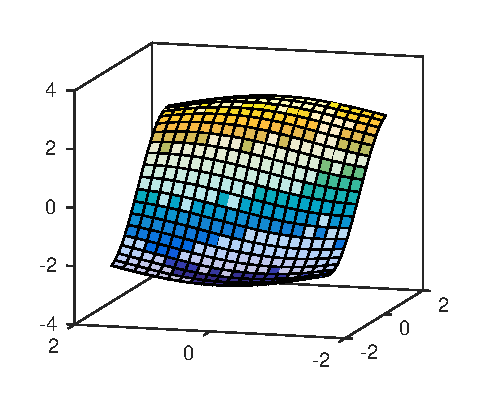
\includegraphics{plots/conclusions/robot_like_extended_mix/phi_approx.eps}
		%\caption{$\hat{W}_\varphi(t)$}
	\end{subfigure}
	\begin{subfigure}{0.5\textwidth}
		% This file was created by matlab2tikz.
%
\definecolor{mycolor1}{rgb}{0.00000,0.44700,0.74100}%
%
\begin{tikzpicture}

\begin{axis}[%
width=0.761\textwidth,
height=0.65\textwidth,
at={(0\textwidth,0\textwidth)},
scale only axis,
xmin=-2,
xmax=2,
ymin=0.075,
ymax=0.11,
axis background/.style={fill=white},
xmajorgrids,
ymajorgrids
]
\addplot [color=red, dashed, line width=1.2pt, forget plot]
  table[row sep=crcr]{%
-1.5707963267949	0.075\\
-1.55500942903816	0.0754735872604091\\
-1.53922253128143	0.0759470564929443\\
-1.5234356335247	0.0764202896991467\\
-1.50764873576797	0.0768931689393802\\
-1.49186183801123	0.0773655763622243\\
-1.4760749402545	0.0778373942338454\\
-1.46028804249777	0.0783085049673383\\
-1.44450114474104	0.0787787911520315\\
-1.4287142469843	0.0792481355827486\\
-1.41292734922757	0.0797164212890175\\
-1.39714045147084	0.080183531564223\\
-1.38135355371411	0.0806493499946915\\
-1.36556665595737	0.0811137604887046\\
-1.34977975820064	0.0815766473054307\\
-1.33399286044391	0.0820378950837711\\
-1.31820596268717	0.0824973888711092\\
-1.30241906493044	0.0829550141519604\\
-1.28663216717371	0.0834106568765104\\
-1.27084526941698	0.0838642034890401\\
-1.25505837166024	0.0843155409562251\\
-1.23927147390351	0.0847645567953064\\
-1.22348457614678	0.0852111391021234\\
-1.20769767839005	0.0856551765790028\\
-1.19191078063331	0.0860965585624964\\
-1.17612388287658	0.0865351750509603\\
-1.16033698511985	0.0869709167319702\\
-1.14455008736312	0.087403675009564\\
-1.12876318960638	0.0878333420313063\\
-1.11297629184965	0.0882598107151674\\
-1.09718939409292	0.0886829747762105\\
-1.08140249633619	0.0891027287530801\\
-1.06561559857945	0.0895189680342852\\
-1.04982870082272	0.0899315888842705\\
-1.03404180306599	0.0903404884692698\\
-1.01825490530925	0.090745564882934\\
-1.00246800755252	0.0911467171717286\\
-0.986681109795789	0.0915438453600932\\
-0.970894212039057	0.0919368504753575\\
-0.955107314282324	0.0923256345724077\\
-0.939320416525591	0.0927101007580959\\
-0.923533518768859	0.0930901532153884\\
-0.907746621012126	0.0934656972272454\\
-0.891959723255394	0.0938366392002258\\
-0.876172825498661	0.0942028866878132\\
-0.860385927741928	0.0945643484134556\\
-0.844599029985196	0.0949209342933129\\
-0.828812132228463	0.0952725554587083\\
-0.81302523447173	0.0956191242782755\\
-0.797238336714998	0.0959605543797992\\
-0.781451438958265	0.09629676067174\\
-0.765664541201532	0.0966276593644415\\
-0.7498776434448	0.0969531679910123\\
-0.734090745688067	0.0972732054278785\\
-0.718303847931335	0.0975876919150013\\
-0.702516950174602	0.0978965490757551\\
-0.686730052417869	0.0981996999364602\\
-0.670943154661137	0.0984970689455667\\
-0.655156256904404	0.0987885819924834\\
-0.639369359147671	0.0990741664260473\\
-0.623582461390939	0.0993537510726306\\
-0.607795563634206	0.0996272662538779\\
-0.592008665877474	0.0998946438040718\\
-0.576221768120741	0.100155817087121\\
-0.560434870364008	0.100410721013169\\
-0.544647972607276	0.100659292054812\\
-0.528861074850543	0.100901468262937\\
-0.513074177093811	0.101137189282154\\
-0.497287279337078	0.101366396365844\\
-0.481500381580345	0.101589032390796\\
-0.465713483823613	0.101805041871446\\
-0.44992658606688	0.102014370973703\\
-0.434139688310147	0.102216967528364\\
-0.418352790553415	0.102412781044123\\
-0.402565892796682	0.102601762720145\\
-0.386778995039949	0.102783865458235\\
-0.370992097283217	0.102959043874573\\
-0.355205199526484	0.103127254311025\\
-0.339418301769752	0.103288454846023\\
-0.323631404013019	0.103442605305015\\
-0.307844506256286	0.103589667270475\\
-0.292057608499554	0.103729604091478\\
-0.276270710742821	0.103862380892834\\
-0.260483812986088	0.103987964583781\\
-0.244696915229356	0.10410632386623\\
-0.228910017472623	0.104217429242566\\
-0.21312311971589	0.104321253023001\\
-0.197336221959158	0.104417769332472\\
-0.181549324202425	0.104506954117091\\
-0.165762426445693	0.10458878515014\\
-0.14997552868896	0.10466324203761\\
-0.134188630932227	0.104730306223284\\
-0.118401733175495	0.10478996099336\\
-0.102614835418762	0.10484219148062\\
-0.0868279376620293	0.10488698466813\\
-0.0710410399052968	0.10492432939249\\
-0.0552541421485642	0.104954216346611\\
-0.0394672443918316	0.104976638082038\\
-0.023680346635099	0.104991589010804\\
-0.00789344887836618	0.104999065406825\\
0.0078934488783664	0.104999065406825\\
0.023680346635099	0.104991589010804\\
0.0394672443918316	0.104976638082038\\
0.0552541421485642	0.104954216346611\\
0.071041039905297	0.10492432939249\\
0.0868279376620296	0.10488698466813\\
0.102614835418762	0.10484219148062\\
0.118401733175495	0.10478996099336\\
0.134188630932227	0.104730306223284\\
0.14997552868896	0.10466324203761\\
0.165762426445693	0.10458878515014\\
0.181549324202425	0.104506954117091\\
0.197336221959158	0.104417769332472\\
0.21312311971589	0.104321253023001\\
0.228910017472623	0.104217429242566\\
0.244696915229356	0.10410632386623\\
0.260483812986088	0.103987964583781\\
0.276270710742821	0.103862380892834\\
0.292057608499554	0.103729604091478\\
0.307844506256286	0.103589667270475\\
0.323631404013019	0.103442605305015\\
0.339418301769752	0.103288454846023\\
0.355205199526484	0.103127254311025\\
0.370992097283217	0.102959043874573\\
0.386778995039949	0.102783865458235\\
0.402565892796682	0.102601762720145\\
0.418352790553415	0.102412781044123\\
0.434139688310147	0.102216967528364\\
0.44992658606688	0.102014370973703\\
0.465713483823612	0.101805041871446\\
0.481500381580345	0.101589032390796\\
0.497287279337078	0.101366396365844\\
0.51307417709381	0.101137189282154\\
0.528861074850543	0.100901468262937\\
0.544647972607275	0.100659292054812\\
0.560434870364008	0.100410721013169\\
0.576221768120741	0.100155817087121\\
0.592008665877473	0.0998946438040718\\
0.607795563634206	0.0996272662538779\\
0.623582461390939	0.0993537510726306\\
0.639369359147671	0.0990741664260473\\
0.655156256904404	0.0987885819924834\\
0.670943154661137	0.0984970689455667\\
0.686730052417869	0.0981996999364602\\
0.702516950174602	0.0978965490757551\\
0.718303847931335	0.0975876919150013\\
0.734090745688067	0.0972732054278785\\
0.7498776434448	0.0969531679910123\\
0.765664541201533	0.0966276593644415\\
0.781451438958265	0.09629676067174\\
0.797238336714998	0.0959605543797992\\
0.81302523447173	0.0956191242782755\\
0.828812132228463	0.0952725554587083\\
0.844599029985196	0.0949209342933129\\
0.860385927741928	0.0945643484134556\\
0.876172825498661	0.0942028866878132\\
0.891959723255393	0.0938366392002258\\
0.907746621012126	0.0934656972272454\\
0.923533518768859	0.0930901532153884\\
0.939320416525591	0.0927101007580959\\
0.955107314282324	0.0923256345724077\\
0.970894212039056	0.0919368504753575\\
0.986681109795789	0.0915438453600932\\
1.00246800755252	0.0911467171717287\\
1.01825490530925	0.090745564882934\\
1.03404180306599	0.0903404884692698\\
1.04982870082272	0.0899315888842705\\
1.06561559857945	0.0895189680342852\\
1.08140249633619	0.0891027287530801\\
1.09718939409292	0.0886829747762105\\
1.11297629184965	0.0882598107151674\\
1.12876318960638	0.0878333420313063\\
1.14455008736312	0.087403675009564\\
1.16033698511985	0.0869709167319702\\
1.17612388287658	0.0865351750509603\\
1.19191078063331	0.0860965585624964\\
1.20769767839005	0.0856551765790029\\
1.22348457614678	0.0852111391021234\\
1.23927147390351	0.0847645567953063\\
1.25505837166024	0.0843155409562251\\
1.27084526941698	0.0838642034890401\\
1.28663216717371	0.0834106568765104\\
1.30241906493044	0.0829550141519604\\
1.31820596268717	0.0824973888711093\\
1.33399286044391	0.0820378950837711\\
1.34977975820064	0.0815766473054308\\
1.36556665595737	0.0811137604887046\\
1.38135355371411	0.0806493499946915\\
1.39714045147084	0.080183531564223\\
1.41292734922757	0.0797164212890175\\
1.4287142469843	0.0792481355827485\\
1.44450114474104	0.0787787911520315\\
1.46028804249777	0.0783085049673383\\
1.4760749402545	0.0778373942338454\\
1.49186183801123	0.0773655763622243\\
1.50764873576797	0.0768931689393802\\
1.5234356335247	0.0764202896991467\\
1.53922253128143	0.0759470564929443\\
1.55500942903816	0.0754735872604091\\
1.5707963267949	0.075\\
};
\addplot [color=mycolor1, line width=1.2pt, forget plot]
  table[row sep=crcr]{%
-1.5707963267949	0.0763353601750211\\
-1.55500942903816	0.0770116398569971\\
-1.53922253128143	0.0776625726099755\\
-1.5234356335247	0.078287708114814\\
-1.50764873576797	0.0788868258348155\\
-1.49186183801123	0.0794599250613931\\
-1.4760749402545	0.0800072127730787\\
-1.46028804249777	0.0805290895358186\\
-1.44450114474104	0.0810261337033189\\
-1.4287142469843	0.0814990842020914\\
-1.41292734922757	0.0819488222061717\\
-1.39714045147084	0.0823763520207806\\
-1.38135355371411	0.0827827815021107\\
-1.36556665595737	0.0831693023417554\\
-1.34977975820064	0.0835371705390093\\
-1.33399286044391	0.0838876873724555\\
-1.31820596268717	0.0842221811641821\\
-1.30241906493044	0.0845419901060491\\
-1.28663216717371	0.0848484463881813\\
-1.27084526941698	0.0851428618359883\\
-1.25505837166024	0.0854265152242616\\
-1.23927147390351	0.0857006413961659\\
-1.22348457614678	0.0859664222721449\\
-1.20769767839005	0.0862249797899084\\
-1.19191078063331	0.0864773707727625\\
-1.17612388287658	0.0867245836806016\\
-1.16033698511985	0.0869675371568929\\
-1.14455008736312	0.0872070802468937\\
-1.12876318960638	0.0874439941280104\\
-1.11297629184965	0.0876789951634298\\
-1.09718939409292	0.0879127390655757\\
-1.08140249633619	0.0881458259371241\\
-1.06561559857945	0.0883788059446357\\
-1.04982870082272	0.0886121853735876\\
-1.03404180306599	0.0888464328137981\\
-1.01825490530925	0.0890819852308763\\
-1.00246800755252	0.0893192536921562\\
-0.986681109795789	0.0895586285342369\\
-0.970894212039057	0.0898004837832066\\
-0.955107314282324	0.0900451806672473\\
-0.939320416525591	0.0902930700938336\\
-0.923533518768859	0.0905444939992893\\
-0.907746621012126	0.0907997855161339\\
-0.891959723255394	0.0910592679424483\\
-0.876172825498661	0.0913232525364064\\
-0.860385927741928	0.0915920351971604\\
-0.844599029985196	0.0918658921294381\\
-0.828812132228463	0.0921450746225776\\
-0.81302523447173	0.0924298031044294\\
-0.797238336714998	0.0927202606558185\\
-0.781451438958265	0.0930165861914287\\
-0.765664541201532	0.093318867527515\\
-0.7498776434448	0.0936271345653795\\
-0.734090745688067	0.0939413528218318\\
-0.718303847931335	0.0942614175338117\\
-0.702516950174602	0.0945871485540729\\
-0.686730052417869	0.0949182862385461\\
-0.670943154661137	0.0952544885041189\\
-0.655156256904404	0.0955953292086224\\
-0.639369359147671	0.0959402979734737\\
-0.623582461390939	0.096288801534465\\
-0.607795563634206	0.0966401666684973\\
-0.592008665877474	0.0969936447045734\\
-0.576221768120741	0.0973484175870897\\
-0.560434870364008	0.0977036054194274\\
-0.544647972607276	0.0980582753770494\\
-0.528861074850543	0.0984114518427706\\
-0.513074177093811	0.0987621275835136\\
-0.497287279337078	0.0991092757585674\\
-0.481500381580345	0.0994518625248981\\
-0.465713483823613	0.0997888599860738\\
-0.44992658606688	0.10011925921838\\
-0.434139688310147	0.100442083101095\\
-0.418352790553415	0.100756398677868\\
-0.402565892796682	0.101061328782793\\
-0.386778995039949	0.101356062677904\\
-0.370992097283217	0.101639865468298\\
-0.355205199526484	0.101912086086306\\
-0.339418301769752	0.102172163666714\\
-0.323631404013019	0.102419632170105\\
-0.307844506256286	0.102654123150203\\
-0.292057608499554	0.102875366602778\\
-0.276270710742821	0.103083189877095\\
-0.260483812986088	0.103277514675175\\
-0.244696915229356	0.103458352208096\\
-0.228910017472623	0.103625796621187\\
-0.21312311971589	0.103780016840236\\
-0.197336221959158	0.103921247027736\\
-0.181549324202425	0.104049775870828\\
-0.165762426445693	0.104165934950196\\
-0.14997552868896	0.104270086461002\\
-0.134188630932227	0.104362610572516\\
-0.118401733175495	0.104443892721963\\
-0.102614835418762	0.104514311140052\\
-0.0868279376620293	0.104574224900636\\
-0.0710410399052968	0.104623962775029\\
-0.0552541421485642	0.104663813152952\\
-0.0394672443918316	0.104694015267359\\
-0.023680346635099	0.104714751930039\\
-0.00789344887836618	0.104726143949625\\
0.0078934488783664	0.104728246364309\\
0.023680346635099	0.104721046579082\\
0.0394672443918316	0.104704464452689\\
0.0552541421485642	0.104678354333811\\
0.071041039905297	0.104642509000242\\
0.0868279376620296	0.104596665410272\\
0.102614835418762	0.104540512132969\\
0.118401733175495	0.10447369828477\\
0.134188630932227	0.104395843764531\\
0.14997552868896	0.104306550548884\\
0.165762426445693	0.104205414785019\\
0.181549324202425	0.104092039399538\\
0.197336221959158	0.103966046930115\\
0.21312311971589	0.103827092281737\\
0.228910017472623	0.103674875111292\\
0.244696915229356	0.103509151553189\\
0.260483812986088	0.103329745014323\\
0.276270710742821	0.103136555788579\\
0.292057608499554	0.10292956926873\\
0.307844506256286	0.102708862566297\\
0.323631404013019	0.102474609386887\\
0.339418301769752	0.102227083048871\\
0.355205199526484	0.101966657575951\\
0.370992097283217	0.101693806838215\\
0.386778995039949	0.101409101760603\\
0.402565892796682	0.101113205661226\\
0.418352790553415	0.10080686782373\\
0.434139688310147	0.100490915446745\\
0.44992658606688	0.100166244148665\\
0.465713483823612	0.0998338072365776\\
0.481500381580345	0.0994946039735112\\
0.497287279337078	0.0991496670976825\\
0.51307417709381	0.098800049860639\\
0.528861074850543	0.098446812857908\\
0.544647972607275	0.098091010925801\\
0.560434870364008	0.097733680371481\\
0.576221768120741	0.097375826790474\\
0.592008665877473	0.0970184137068851\\
0.607795563634206	0.0966623522471626\\
0.623582461390939	0.0963084920290207\\
0.639369359147671	0.0959576134138277\\
0.655156256904404	0.0956104212342782\\
0.670943154661137	0.0952675400704223\\
0.686730052417869	0.0949295111071345\\
0.702516950174602	0.0945967905658655\\
0.718303847931335	0.0942697496640811\\
0.734090745688067	0.0939486760181306\\
0.7498776434448	0.0936337763703602\\
0.765664541201533	0.093325180489972\\
0.781451438958265	0.0930229460702001\\
0.797238336714998	0.0927270644225132\\
0.81302523447173	0.0924374667522789\\
0.828812132228463	0.0921540307900495\\
0.844599029985196	0.0918765875485841\\
0.860385927741928	0.0916049279779948\\
0.876172825498661	0.0913388092999164\\
0.891959723255393	0.0910779608161175\\
0.907746621012126	0.0908220890071033\\
0.923533518768859	0.0905708817614841\\
0.939320416525591	0.0903240116065301\\
0.955107314282324	0.0900811378436435\\
0.970894212039056	0.0898419075285739\\
0.986681109795789	0.0896059552741668\\
1.00246800755252	0.0893729018922575\\
1.01825490530925	0.0891423519300242\\
1.03404180306599	0.0889138901936683\\
1.04982870082272	0.0886870773877212\\
1.06561559857945	0.0884614450306688\\
1.08140249633619	0.0882364898360599\\
1.09718939409292	0.088011667772083\\
1.11297629184965	0.0877863880311\\
1.12876318960638	0.0875600071532956\\
1.14455008736312	0.0873318235550763\\
1.16033698511985	0.0871010727128922\\
1.17612388287658	0.0868669232467062\\
1.19191078063331	0.0866284741344904\\
1.20769767839005	0.0863847532701215\\
1.22348457614678	0.0861347175523112\\
1.23927147390351	0.0858772546622396\\
1.25505837166024	0.0856111866530684\\
1.27084526941698	0.0853352754362537\\
1.28663216717371	0.0850482302084269\\
1.30241906493044	0.0847487168195271\\
1.31820596268717	0.0844353690388182\\
1.33399286044391	0.0841068016314415\\
1.34977975820064	0.0837616251152466\\
1.36556665595737	0.0833984620268029\\
1.38135355371411	0.0830159644876634\\
1.39714045147084	0.0826128328280016\\
1.41292734922757	0.0821878349954544\\
1.4287142469843	0.0817398264530434\\
1.44450114474104	0.0812677702519624\\
1.46028804249777	0.080770756953219\\
1.4760749402545	0.080248024066853\\
1.49186183801123	0.0796989746788395\\
1.50764873576797	0.0791231949437749\\
1.5234356335247	0.0785204701358242\\
1.53922253128143	0.0778907989708555\\
1.55500942903816	0.0772344059387022\\
1.5707963267949	0.0765517514154707\\
};
\end{axis}
\end{tikzpicture}%
		%\caption{$\hat{W}_\gamma(t)$)}
	\end{subfigure}
	\caption{Προσεγγίσεις των συναρτήσεων $\varphi(x)$ (αριστερά) και $\gamma(x)$ (δεξιά) στο παράδειγμα \ref{subsec:mixed_order}}
	\label{fig:robot_like_extended_mix_approximations}
\end{figure}

\subsubsection{Αποτελέσματα}
Το σύστημα κλειστού βρόγχου με την τροχιά αναφοράς που περιγράψαμε στην προηγούμενη παράγραφο προσομοιώθηκε για 100 επαναλήψεις. Στο Σχήμα \ref{fig:robot_like_extended_mix_w_conv} δίνεται η χρονική εξέλιξη κάποιων βαρών $\hat{\varphi}(t)$ και $\hat{\gamma}(t)$, απ' όπου είναι προφανές πως και εδώ, 100 περίοδοι είναι αρκετές έτσι ώστε τα βάρη να σταθεροποιηθούν.

Τα αποτελέσματα των προσεγγίσεων παρουσιάζονται στο Σχήμα \ref{fig:robot_like_extended_mix_approximations}. Όπως φαίνεται λοιπόν, σε αυτή την περίπτωση το σχήμα αναγνώρισης καταφέρνει να προσεγγίσει ικανοποιητικά και τις δυο άγνωστες συναρτήσεις $\varphi(x)$ και $\gamma(x)$ σε όλο το σύνολο αναγνώρισης $\Omega_x$.

\subsection{Συμπέρασμα}
Το συμπέρασμα που μπορούμε να βγάλουμε από τα παραπάνω πειράματα είναι πως το πρόβλημα οφείλεται στα επίπεδα διέγερσης $\alpha_0$ και $\alpha_1$. Παρόλο που και στις τρεις περιπτώσεις πειραμάτων ικανοποιείται η ΣΕΔ της Ενότητας \ref{subsec:rbf_PE}, μέσω αυτών των πειραμάτων επαληθεύεται πως η ικανοποίηση της συνθήκης δεν εξασφαλίζει πως τα βάρη των νευρωνικών δικτύων θα συγκλίνουν στο βέλτιστο αποτέλεσμα, αλλά σε μια περιοχή αυτού, το πλάτος της οποίας εξαρτάται από τα επίπεδα διέγερσης. Δυστυχώς η διατύπωση της συνθήκης αυτής είναι πολύ αφηρημένη για να υποδεικνύει τι προδιαγραφές πρέπει να πληρεί μια τροχιά αναφοράς για να επιτυγχάνει υψηλά επίπεδα διέγερσης.

\begin{figure}
	\centering
	\documentclass{standalone}

\usepackage{tikz}
\usetikzlibrary{shapes,arrows}
\usepackage{standalone}

\usepackage{amsmath}

\begin{document}


%\tikzstyle{block} = [draw, fill=blue!20, rectangle, 
%    minimum height=3em, minimum width=6em]
    
\tikzstyle{block} = [draw, rectangle, 
minimum height=3em, minimum width=6em]
\tikzstyle{sum} = [draw, circle, node distance=2cm]
\tikzstyle{input} = [coordinate]
\tikzstyle{output} = [coordinate]
\tikzstyle{pinstyle} = [pin edge={to-,thin,black}]
\tikzstyle{split} = [draw, fill=black, circle,inner sep=0pt, minimum size=0.12cm ]


%% 
%\tikzstyle{split} = [ \draw[red,thick,dashed], circle (3cm);]

% The block diagram code is probably more verbose than necessary


\begin{tikzpicture}[auto, node distance=2cm,>=latex']
% We start by placing the blocks
\node [input, name=input] at (0,0) {};
%\node [block, right of=input,node distance=4cm] (plant) 
%{ 
%	$\begin{aligned}
%	\dot{x}_1 &= x_2\\
%	\dot{x}_2 &= f(x)g^{-1}(x) + g^{-1}(x)u(t)\\
%	\end{aligned}$
%};
\node [block, label={Plant}]  at (4.5,1) (plant) 
{ 
	$\begin{aligned}
	\dot{x}_1 &= x_2\\
	\dot{x}_2 &= f(x) + g(x)u(t)\\
	\end{aligned}$
};
\node [block, label=below:{Plant Approximation}]  at (4.5,-1) (plant_approx) 
{	$\begin{aligned}
	%\dot{\hat{x}}_1 &= \hat{x}_2\\
	\hat{\gamma}(x) \dot{\hat{x}}_2 &= \hat{\varphi}(x) + u(t)\\
	\end{aligned}$};


\node [sum] at (8,0) (sum) {};
\node [split] at (1,0) (split){};
\node [output] at (9,0) (output) {};


% We draw an edge between the controller and system block to 
% calculate the coordinate u. We need it to place the measurement block. 
\draw [->] (input) -- node[name=u] {$u(t)$} (split);

% Once the nodes are placed, connecting them is easy. 
\draw [draw,->] (split) |-  (plant_approx.west);
\draw [draw,->] (split) |-  (plant);
\draw [draw,->] (plant.east) -| node[anchor=south] {$x_2(t)$} node[pos=0.99,anchor=east] {$+$} (sum);
\draw [draw,->] (plant_approx) -| node[anchor=north] {$\hat{x}_2(t)$}  node[pos=0.99] {$-$} (sum);

%\draw [draw,->] (plant.east)-(0,2mm) --+ (10mm,0) -|+(0,-3mm)  (plant_approx);
\draw [draw,->] (plant.east)+(0,-3mm) -| +(5mm,-3mm) -- +(5mm,-10mm) -- +(-43mm,-10mm) node[pos=0.99,anchor=east] {$x(t)$} -- +(-43mm,-17mm) -- +(-40.5mm,-17mm); 
%node[anchor=south] {$x_3(t)$}  (sum);

\draw [->] (sum) -- node[name=u] {$e(t)$} (output);

%\draw [draw,->] (plant_approx) |-  (plant_approx);

%\draw [->] (system) -- node [name=y] {$y$}(output);
%\draw [->] (y) |- (measurements);
%\draw [->] (measurements) -| node[pos=0.99] {$-$} 

\end{tikzpicture}

\end{document}
	\caption{Αρχιτεκτονική αξιολόγησης δευτεροβάθμιου συστήματος}
	\label{fig:validation_schema}
\end{figure}

\section{Αξιολόγηση Συστημάτων}
Μέχρι στιγμής, σε όλα τα πειράματα του Κεφαλαίου \ref{chap:experiments} η αξιολόγηση των προσεγγίσεων που παρήγαγε το σχήμα αναγνώριση γινόταν μέσω απευθείας σύγκρισης των προσεγγίσεων με τις πραγματικές συναρτήσεις. Ωστόσο, η μέθοδος αυτή στην πραγματικότητα δεν είναι εφικτή αφού οι άγνωστες συναρτήσεις δεν είναι διαθέσιμες προς μέτρηση, αλλά εκφράζονται μέσω της δυναμικής του συστήματος προς αναγνώριση.

Σε αυτή την Ενότητα παρουσιάζουμε έναν τρόπο αξιολόγησης των εκτιμήσεων, που δεν χρησιμοποιεί γνώσεις των συναρτήσεων του συστήματος αλλά βασίζεται στην δημιουργία ενός μοντέλου αυτού με βάση τις εκτιμήσεις.

Η λογική που ακολουθείται απεικονίζεται στο Σχήμα \ref{fig:validation_schema} για την αξιολόγηση ενός δευτεροβάθμιου συστήματος. Όπως φαίνεται, χρησιμοποιώντας τις εκτιμήσεις $\hat{\varphi}(x)$ και $\hat{\gamma}(x)$ κατασκευάζουμε την διαφορική εξίσωση:
\begin{equation}
	\hat{\gamma}(x) \dot{\hat{x}}_2(t) = \hat{\varphi}(x) + u(t), 
	\quad x \in \Omega_x
	\label{eq:eval_DE}
\end{equation}
, όπου $x$ το διάνυσμα των πραγματικών καταστάσεων το οποίο είναι μετρήσιμο. Εάν οι προσεγγίσεις βρίσκονται κοντά στις πραγματικές συναρτήσεις, τότε η συμπεριφορά του δυναμικού συστήματος~\eqref{eq:eval_DE} θα είναι πολύ παρόμοια με αυτή του πραγματικού δυναμικού συστήματος

\subsection{Επιλογή του $u(t)$}
Ένα από τα προβλήματα της παρούσας μεθοδολογίας είναι η επιλογή της εισόδου ελέγχου $u(t)$. Συγκεκριμένα το πρόβλημα οφείλεται στο γεγονός ότι μια αυθαίρετη επιλογή της εισόδου ελέγχου ενδέχεται να οδηγήσει πολύ σύντομα την τροχιά $x(t)$ εκτός του συνόλου αναγνώρισης $\Omega_x$, έξω από το οποίο δεν έχει νόημα η διαδικασία αξιολόγησης του συστήματος. Παρακάτω παρουσιάζουμε δυο πιθανές επιλογές της εισόδου ελέγχου οι οποίες αντιμετωπίζουν το πρόβλημα που προαναφέρθηκε

\subsubsection{Γραμμικοποίηση του συστήματος μέσω ανάδρασης}
Η πρώτη λύση είναι η επιλογή του $u(t)$ έτσι ώστε να γραμμικοποιεί το πραγματικό σύστημα. Μια τέτοια είσοδος είναι η
\begin{equation}
	u(t) =  \frac{- f(x) + \nu(t)}{g(x)}
	\label{eq:evaluation_control_input}
\end{equation}
όπου $\nu(t)$ μια νέα είσοδος αναφοράς η οποία σχεδιάζεται με βάση την επιθυμητή τροχιά του γραμμικοποιημένου συστήματος. Αντικαθιστώντας την εξίσωση \ref{eq:evaluation_control_input} στο μοντέλο αναφοράς \ref{eq:eval_DE} προκύπτει:
\begin{equation}
	\hat{\gamma}(x) \dot{\hat{x}}_2(t) = -\tilde{\varphi}(x) + \gamma(x) \nu(t)
\end{equation}
ενώ με αντικατάσταση της ίδιας εισόδου στο πραγματικό σύστημα έχουμε:
\begin{equation}
\dot{x}_2(t) = \nu(t)
\end{equation}
Τέλος, ορίζοντας το σφάλμα παρακολούθησης των δυο καταστάσεων ως $\tilde{x}_2 = x_2 - \hat{x}_2$, μπορούμε να γράψουμε την δυναμική του σφάλματος ώς:
\begin{equation}
	\hat{\gamma}(x) \dot{\tilde{x}} = -\tilde{\varphi}(x)  -\tilde{\gamma}(x) \nu(t)
	\label{eq:evaluation_error_DE_1}
\end{equation}
Καθώς γνωρίζουμε τις αρχικές συνθήκες του πραγματικού συστήματος, και είμαστε σε θέση να επιλέξουμε τις αρχικές συνθήκες του συστήματος αναφοράς, μπορούμε να επιλέξουμε το $\hat{x}_2(0) = x_2(0)$ επιτυγχάνοντας έτσι $\tilde{x}_2(0) = 0$. Όπως είναι προφανές, εάν τα παραμετρικά σφάλματα $\tilde{\varphi}(x)$ και $\tilde{\gamma}(x)$ είναι ίσα με το $0$, τότε το σφάλμα $\tilde{x}$ θα παραμείνει ίσο με το $0$ καθ' όλη την διάρκεια της διαδικασίας αξιολόγησης.\\
\begin{remark}
	Παρατηρώντας την εξίσωση \ref{eq:evaluation_control_input}, φαίνεται πως και εδώ κάνουμε χρήση των άγνωστων συναρτήσεων $f(x)$ και $g(x)$. Η λογική πίσω από αυτή την επιλογή είναι ότι  ένα πραγματικό σύστημα το οποίο μας είναι άγνωστο, συνήθως συνοδεύεται από κάποιον ελεγκτή ο οποίος μπορεί να το οδηγήσει σε επιθυμητές τροχιές. Ωστόσο, καθώς τα συστήματα που μελετάμε είναι ακαδημαϊκά και δεν υπάρχει κάποιος τέτοιος μηχανισμός, επιλέγουμε καταχρηστικά την είσοδο ελέγχου της εξίσωσης \ref{eq:evaluation_control_input}. Σε μια πραγματική εφαρμογή θα χρησιμοποιούσαμε το σήμα ελέγχου του ελεγκτή που συνοδεύει το σύστημα.
\end{remark}

\subsubsection{Χρήση των εκτιμήσεων για γραμμικοποίηση}
Η δεύτερη εναλλακτική είναι η επιλογή μιας εισόδου ελέγχου που να χρησιμοποιεί τις εκτιμήσεις $\hat{\varphi}(x)$ και $\hat{\gamma}(x)$ για να γραμμικοποιήσει το άγνωστο σύστημα. Κατά συνέπεια, επιλέγουμε την είσοδο ελέγχου ως:
\begin{equation}
	u(t) = -\hat{\varphi}(x) + \hat{\gamma}(x) \nu(t)
	\label{eq:evaluation_control_input_alt}
\end{equation}
Ακολουθώντας παρόμοια μεθοδολογία με πριν, αντικαθιστώντας την εξίσωση \ref{eq:evaluation_control_input_alt} στο μοντελοποιημένο και στο πραγματικό σύστημα καταλήγουμε την διαφορική εξίσωση του σφάλματος $\tilde{x}$:
\begin{equation}
	\dot{\tilde{x}} = g(x) \left( \tilde{\varphi}(x)  -\tilde{\gamma}(x) \nu(t) \right)
	\label{eq:evaluation_error_DE_2}
\end{equation}
η οποία επίσης προσφέρει την ιδιότητα να αυξάνεται ανάλογα με την ποσότητα των παραμετρικών σφαλμάτων $\tilde{\varphi}(x)$ και $\tilde{\gamma}(x)$. Συγκρίνοντας τις εξισώσεις \ref{eq:evaluation_error_DE_1} και \ref{eq:evaluation_error_DE_2} παρατηρούμε ότι η δομή τους είναι πολύ παρόμοια, συνεπώς ακόμα και στην περίπτωση που δεν μπορούμε να διατηρεί την τροχιά του πραγματικού συστήματος εντός του $\Omega_x$, μπορούμε να χρησιμοποιήσουμε την εναλλακτική είσοδο αναφοράς που παρουσιάζεται σε αυτή την υποενότητα. Εάν η τροχιά $x(t)$ οδηγηθεί σε σύντομο χρονικό διάστημα εκτός του $\Omega_x$ τότε μπορούμε να βγάλουμε το συμπέρασμα πως η αναγνώριση δεν είναι επαρκής.


\subsection{Αποτελέσματα Αξιολόγησης}
Στην παρούσα ενότητα θα χρησιμοποιήσουμε το σύστημα αναγνώρισης που παρουσιάστηκε για να αξιολογήσουμε τα αποτελέσματα αναγνώρισης πραγματικών συστημάτων που παρουσιάζονται στο Κεφάλαιο \ref{chap:experiments}. Σε όλα τα πειράματα θα χρησιμοποιήσουμε την αρχιτεκτονική αξιολόγησης του σχήματος \ref{fig:validation_schema} και θα επιλέξουμε την είσοδο ελέγχου της εξίσωσης~\eqref{eq:evaluation_control_input}, δηλαδή της εισόδου που γραμμικοποιεί το πραγματικό σύστημα.

\subsubsection{Φαινόμενο Wing Rock}
Για την αξιολόγηση των προσεγγίσεων $\hat{\varphi}(x)$ και $\hat{\gamma}(x)$ πρέπει αρχικά να σχεδιάσουμε την είσοδο του γραμικοποιημένου συστήματος $\nu(t)$ έτσι ώστε να εξερευνεί επαρκώς το σύνολο αναγνώρισης $\Omega_x$. Στο συγκεκριμένο πρόβλημα το $\Omega_x$ επιλέγεται ως το σύνολο $\bmqty{-\frac{\pi}{4},\frac{\pi}{4}} \times \bmqty{-\frac{\pi}{4},\frac{\pi}{4}}$. Επιλέγουμε την είσοδο ελέγχου $\nu(t)$ ως 
\begin{equation}
\nu(t) = -(b/a)^2 x_1(t) - K \frac{x_2(t)}{\| x(t) \|}
\label{eq:ref_control_input}
\end{equation}
όπου $b$, $a$ θετικές σταθερές. Η σταθερά $K$ μπορεί να είναι θετική, αρνητική ή μηδέν. Με κατάλληλη επιλογή των σταθερών αυτών, καθώς και των αρχικών συνθηκών του πραγματικού συστήματος, η επιλογή της εξίσωσης~\eqref{eq:ref_control_input} παράγει μια ελλειψοειδή τροχιά η οποία παρουσιάζεται στο Σχήμα \ref{fig:ellipse_traj}. Για θετικές τιμές του $K$ το βήμα της έλλειψης είναι αρνητικό, δηλαδή η ακτίνα μειώνεται συναρτήσει του χρόνου, ενώ για αρνητικές τιμές το βήμα είναι θετικό. Τέλος, για επιλογή του $K = 0$ η τροχιά του συστήματος αναφοράς θα είναι μια κλειστή έλλειψη. Στο συγκεκριμένο παράδειγμα έχουμε επιλέξει $a = b = 1$ και $Κ = 0.03$, αλλά η ίδια είσοδος αναφοράς μπορεί να επιλεχθεί έτσι ώστε να καλύψει οποιοδήποτε τετραγωνικό σύνολο αναγνώρισης.

\begin{figure}
	\centering
	% This file was created by matlab2tikz.
%
\definecolor{mycolor1}{rgb}{0.00000,0.44700,0.74100}%
%
\begin{tikzpicture}

\begin{axis}[%
width=0.38\textwidth,
height=0.4\textwidth,
at={(0\textwidth,0\textwidth)},
scale only axis,
xmin=-1.28539816339745,
xmax=1.28539816339745,
xlabel style={font=\color{white!15!black}},
xlabel={$x_1$},
ymin=-1.28539816339745,
ymax=1.28539816339745,
ylabel style={font=\color{white!15!black}},
ylabel={$x_2$},
axis background/.style={fill=white},
xmajorgrids,
ymajorgrids,
legend style={legend cell align=left, align=left, draw=white!15!black}
]
\addplot [color=mycolor1, line width=1.2pt]
  table[row sep=crcr]{%
0	0.784398163397448\\
0.0273219403516642	0.782875601772499\\
0.0620415452570837	0.77955883497545\\
0.0965796429115783	0.774707799159662\\
0.137893959332093	0.766834289993355\\
0.161863801216344	0.761208639038409\\
0.185645493451139	0.754840107245956\\
0.209215842145248	0.747735886954703\\
0.232551891477001	0.739903895483047\\
0.260433137052482	0.729470286738512\\
0.287898761499899	0.718001136991305\\
0.314909817314104	0.705514574274185\\
0.341428071494788	0.692030162372207\\
0.367416054696718	0.677568860634287\\
0.392837116469228	0.662153002357787\\
0.421828384546732	0.642925237941538\\
0.449937940071074	0.622462071154313\\
0.47711184072252	0.600806143841176\\
0.509469892649363	0.572326834309502\\
0.536487201246523	0.545999206434109\\
0.562202851578022	0.518447646600506\\
0.588364457452339	0.487497656704654\\
0.614561283114107	0.452959977007048\\
0.638796939824049	0.417093780761568\\
0.661000598550869	0.380013307162373\\
0.679394676403872	0.345295913403541\\
0.694288774701231	0.313660286346884\\
0.707739566201198	0.281440660485576\\
0.721591704614262	0.243151905601481\\
0.733405944838134	0.204265595981603\\
0.742071368068004	0.169737339686272\\
0.74824136349244	0.139785758898587\\
0.753213750354125	0.109659258025593\\
0.757203775960941	0.0772585579409567\\
0.759700046444316	0.0465818487871147\\
0.761099038789923	0.00623157773511029\\
0.7605499432509	-0.0295544665400986\\
0.759161370349695	-0.054579847846266\\
0.756161050876745	-0.0866511273935867\\
0.751802629216431	-0.11851254455099\\
0.74603243080567	-0.15042127782099\\
0.73882277068041	-0.182310144406502\\
0.73023979625189	-0.213802644514762\\
0.719085718926432	-0.24834206167345\\
0.704879473883188	-0.285662770640596\\
0.688711143415934	-0.322097848119242\\
0.670630541191769	-0.357546087964408\\
0.649294006655759	-0.394167424204835\\
0.625916947805765	-0.42943850141759\\
0.599193699360553	-0.464984643181735\\
0.584328315329612	-0.482956224620559\\
0.568907073420533	-0.500430556604478\\
0.552945830420977	-0.517391036377984\\
0.536460956635776	-0.533821585997308\\
0.504429393177665	-0.562950077151032\\
0.474226486708211	-0.587444266182733\\
0.442781280061495	-0.610269021382422\\
0.40904049940864	-0.632060027171632\\
0.372988334039966	-0.652568932912932\\
0.335843995185041	-0.670977572288453\\
0.304137573436554	-0.684677105434109\\
0.271825992727864	-0.696853210925272\\
0.2389810189174	-0.707481857394986\\
0.205675515996524	-0.71654257202695\\
0.171983239350654	-0.724018400896708\\
0.137969413143755	-0.729897266851779\\
0.103718161721439	-0.734166999504528\\
0.0768775285022205	-0.736376432029748\\
0.0284601032097196	-0.737870872984518\\
-0.00812399744385961	-0.736887268676629\\
-0.038212456264312	-0.734713815617992\\
-0.0681869771698878	-0.731314932762384\\
-0.11410568045795	-0.723683523794277\\
-0.154772944907142	-0.714412517600471\\
-0.194851855885034	-0.70287860928777\\
-0.220078332748449	-0.694348919197624\\
-0.244980688455145	-0.684926136619815\\
-0.269526912271584	-0.674623904566867\\
-0.312982403678305	-0.653771258912434\\
-0.350684693060892	-0.632759795079638\\
-0.387093309634082	-0.609627299382605\\
-0.42116207368439	-0.585163435489461\\
-0.452899187223906	-0.559609382549413\\
-0.480693335377738	-0.534738795093319\\
-0.504821058267343	-0.510992959241577\\
-0.527828982398017	-0.486205397108203\\
-0.552004154279478	-0.457532361430997\\
-0.574681125226237	-0.42772096432965\\
-0.595803659787823	-0.396851979147819\\
-0.614740081975299	-0.366008376162904\\
-0.628692616210317	-0.340880091223721\\
-0.641643529352997	-0.315262595874431\\
-0.656787920106416	-0.281685566730282\\
-0.669043835845312	-0.250645690352669\\
-0.679859615619226	-0.219134987050838\\
-0.690096852948539	-0.183907292409731\\
-0.699230958279351	-0.144930896838335\\
-0.706189805610884	-0.105598840026133\\
-0.710808884633474	-0.0676154875332444\\
-0.713330504988297	-0.0311412841664531\\
-0.714002787686631	0.00300494100919424\\
-0.713146217694167	0.035068439398196\\
-0.711130369388302	0.0639711164854156\\
-0.708518176410837	0.0882262696741889\\
-0.704250074767352	0.117373900456449\\
-0.698777093879104	0.146268676159081\\
-0.691741069021998	0.176302650189939\\
-0.684226969583152	0.20322828509875\\
-0.675653913051873	0.229790867148138\\
-0.664439295659825	0.260002443683206\\
-0.651855012316521	0.289611386699618\\
-0.6353743845837	0.323517551920364\\
-0.618271234980946	0.354424236894223\\
-0.599633067021219	0.384364222364477\\
-0.579402714466618	0.413409911892434\\
-0.557612619133681	0.44147199098329\\
-0.534422750563209	0.468327744731409\\
-0.507436487031956	0.496333056713463\\
-0.47632606386565	0.524983043484126\\
-0.44512683666487	0.550394616228775\\
-0.414168368884715	0.572766519216961\\
-0.382026008724411	0.593346834927614\\
-0.3485486633356	0.612209499756833\\
-0.313818894685162	0.629258253704224\\
-0.27819149548134	0.644297619703267\\
-0.260076598735325	0.651050249198365\\
-0.231721579438016	0.660468612605916\\
-0.188539766361699	0.672232105637836\\
-0.144688133307524	0.681141957916882\\
-0.122569158180449	0.684517019600521\\
-0.0927857238892946	0.68790426004382\\
-0.0690887729616337	0.689663786531663\\
-0.0453453976467152	0.690603796882171\\
-0.00197810272060606	0.690207213988617\\
0.0307497199500701	0.688099767279533\\
0.0670335750902218	0.683931354257369\\
0.0910785525774652	0.68009358459589\\
0.127364913493573	0.672645369384835\\
0.163200208128599	0.663278713874398\\
0.180916738236021	0.657885627342266\\
0.207437742735714	0.648836461191954\\
0.233570034699133	0.638733868688705\\
0.259271233355616	0.627596477060576\\
0.284499749065264	0.615444589200196\\
0.30921484805225	0.602300141305528\\
0.328937401060754	0.590877298000772\\
0.348271953182454	0.578825158632157\\
0.382616634689895	0.555161746333174\\
0.412519008933891	0.53195871879696\\
0.44110223243919	0.507203788922597\\
0.468283094353364	0.480975859554221\\
0.493565383362322	0.453831219499739\\
0.514573109094615	0.428898187203103\\
0.534372239899503	0.403047342747566\\
0.555172460733757	0.372907845332655\\
0.574330056047558	0.34177024935273\\
0.583276724617267	0.325855797792951\\
0.596795305162841	0.299748783689202\\
0.61693822390529	0.254751753129771\\
0.630829171386457	0.21741737397084\\
0.642504181983489	0.179430350514601\\
0.652216274283288	0.139573674307624\\
0.659691120784924	0.0979479573745005\\
0.664062867766233	0.0614396663839829\\
0.666206731375602	0.0302286773146901\\
0.666868835634806	-0.00546956760201889\\
0.665942297754547	-0.0355360867946893\\
0.663383684169303	-0.0682039798608896\\
0.659219666938983	-0.100633847598011\\
0.656539752635003	-0.11673503693781\\
0.650681746809567	-0.145656051071556\\
0.643540222468337	-0.174229082867545\\
0.635131866158559	-0.202397899698558\\
0.625475954469514	-0.230107194528535\\
0.614594243425607	-0.257302683251379\\
0.601225104567362	-0.286585901108212\\
0.586434858157437	-0.315112616727064\\
0.57385653585123	-0.336928058661716\\
0.560447074696156	-0.358204511819361\\
0.546227824153156	-0.378911196837194\\
0.531221279134958	-0.399018212261194\\
0.503700244076736	-0.432045773297538\\
0.479099484270455	-0.45809405871756\\
0.453099428134404	-0.482679217303089\\
0.425782894355382	-0.505729602348893\\
0.396475464638766	-0.527716530094644\\
0.369323115648408	-0.545849540182442\\
0.341289922982528	-0.562544741776135\\
0.309200981720733	-0.579359387127329\\
0.276219646063915	-0.594301721042892\\
0.242452355076048	-0.607329132822235\\
0.216032707305345	-0.616017600467276\\
0.189263003196088	-0.623539200654386\\
0.162193869066178	-0.629882026860094\\
0.134876424677612	-0.635036487023436\\
0.10736216395752	-0.638995267505265\\
0.0760676373195929	-0.642025647568289\\
0.0446626728902259	-0.643515828414108\\
0.0206491620504906	-0.643616417437282\\
-0.0181223288257618	-0.641883263366065\\
-0.0475801882581883	-0.638994267027984\\
-0.0802122866597902	-0.63418895908019\\
-0.101811819103277	-0.630064545020139\\
-0.125105618303338	-0.62475621115126\\
-0.148186503249293	-0.618595188531917\\
-0.17102300122657	-0.611591513577376\\
-0.193584034058817	-0.603756374711778\\
-0.215838961000263	-0.595102093873413\\
-0.237757619724125	-0.585642108704612\\
-0.261210671923753	-0.57444048859945\\
-0.284192268686992	-0.562320821903771\\
-0.306665707334095	-0.549304747850777\\
-0.328595202578877	-0.535415366961119\\
-0.349945939605414	-0.520677185525011\\
-0.382088247535286	-0.495994479165511\\
-0.409638680347808	-0.472142471537078\\
-0.435789942855817	-0.446827428765226\\
-0.465012302291552	-0.414872219644983\\
-0.492006115156529	-0.381115881525047\\
-0.516654726655021	-0.345719755550987\\
-0.533287143534918	-0.318630276187706\\
-0.547264081818375	-0.29327295031938\\
-0.558891939052537	-0.269870602913836\\
-0.569544827849939	-0.246055126431597\\
-0.583899111674798	-0.208972796661282\\
-0.594494169191083	-0.176030215991546\\
-0.60358975677869	-0.141241482802651\\
-0.610236542590684	-0.108629109064901\\
-0.614630122212155	-0.0798648240662042\\
-0.618253027080839	-0.0434688510621725\\
-0.619568412360118	-0.0160402953286597\\
-0.619606432233439	0.0144850945204672\\
-0.61806823613264	0.0459206436627165\\
-0.614857874955962	0.0777638344247326\\
-0.609784938582023	0.110512702250438\\
-0.60447852310255	0.136355402913708\\
-0.596908797057691	0.16605947463431\\
-0.587864292303287	0.195276197610107\\
-0.577371207379819	0.223933610961204\\
-0.564204945634416	0.254697423943461\\
-0.549369654795779	0.284609778142748\\
-0.532914590134833	0.313582425514065\\
-0.513441081202122	0.343639993354596\\
-0.494666200477449	0.369276249464237\\
-0.474569745204372	0.393823725468655\\
-0.451206232304811	0.419286645475684\\
-0.428210441079636	0.441654675352012\\
-0.40405499077774	0.462705223957321\\
-0.378811750288531	0.482381424067157\\
-0.352555546158814	0.500630492622709\\
-0.317475321664249	0.521896027737082\\
-0.281022658258266	0.540635724649444\\
-0.243373620949876	0.55676942760304\\
-0.224156893151381	0.563837412701466\\
-0.20214597197974	0.571016421368391\\
-0.179873508320625	0.577321669522437\\
-0.157373560089588	0.582745291292508\\
-0.134680459621458	0.587280764868019\\
-0.111828758934701	0.590922909550573\\
-0.0888531826446801	0.593667903897355\\
-0.0657885786356849	0.595513300011474\\
-0.0411114609604967	0.596489284843028\\
-0.00169766490774192	0.59592270075887\\
0.0295315383722209	0.593617381782716\\
0.06414923098514	0.589125063083658\\
0.08705619638541	0.585014211560966\\
0.119762638732874	0.577534084723291\\
0.151997322772927	0.568246404259254\\
0.16790619870766	0.562935370968709\\
0.192598572387077	0.553700965458252\\
0.216859021580373	0.543403607270322\\
0.240641038954426	0.532065993935016\\
0.263899166478939	0.519712814718159\\
0.285959513517772	0.506759035683882\\
0.307443598355078	0.492897325963644\\
0.328312965313707	0.478155405531305\\
0.348530393392171	0.462562582894885\\
0.368059967565042	0.446149699646902\\
0.386867135030281	0.428949052069622\\
0.412524153800929	0.402960683242624\\
0.42957968029902	0.383817422508493\\
0.455156144467052	0.35171853752595\\
0.47844538074948	0.318038191239019\\
0.495276136191724	0.290214702288035\\
0.510544745743017	0.261584032902156\\
0.525642427932366	0.228897931574057\\
0.539908876442254	0.192035436179612\\
0.551651066214872	0.154423314072886\\
0.560648044420705	0.117092268321753\\
0.567158132239436	0.0793775837907014\\
0.570543758832348	0.0492521263083323\\
0.572341998300575	0.0190733865500862\\
0.572486095859813	-0.0140800986516263\\
0.571517410339929	-0.0361072929242171\\
0.568689389708796	-0.0671757472249642\\
0.564168115604739	-0.0979542576951049\\
0.561278056368473	-0.113206210313332\\
0.551397561187855	-0.153851567987442\\
0.539882332109489	-0.189811810386202\\
0.525990096643401	-0.22479585421719\\
0.516101282376836	-0.246158356429499\\
0.496139275955455	-0.283274885106071\\
0.476169919615253	-0.314695090604862\\
0.454152563461133	-0.34460433288522\\
0.429482255597994	-0.373654628903028\\
0.402117154200842	-0.401565299582878\\
0.372855852048521	-0.427374187443631\\
0.3575615051397	-0.439452148402362\\
0.338302661890267	-0.453440490522026\\
0.318459288184256	-0.466552915342965\\
0.298069659201561	-0.478766872354198\\
0.27717298303011	-0.490061536158937\\
0.255809326411471	-0.500417843048996\\
0.234019539977894	-0.509818524464939\\
0.211845180643504	-0.518248137426607\\
0.190142615142323	-0.525442947843996\\
0.168160105915864	-0.5317120962979\\
0.145936319240406	-0.537046650009423\\
0.105945000687392	-0.544202114029172\\
0.0705928673361972	-0.547999460832402\\
0.0350697225130823	-0.549486844455703\\
-0.00334929406004825	-0.548498667571562\\
-0.0287215386140675	-0.54636575042058\\
-0.0512689231889484	-0.543472949145053\\
-0.0808099942339933	-0.538239664882766\\
-0.107551148070367	-0.532057261756087\\
-0.141046104680486	-0.522304911693415\\
-0.173855493245704	-0.510478195037933\\
-0.206868405563763	-0.496151944032417\\
-0.237019667956755	-0.480766171164768\\
-0.263419997285941	-0.46532164449897\\
-0.288919248459701	-0.44847597852017\\
-0.313492318605146	-0.430245936305775\\
-0.337058902548363	-0.410684650301822\\
-0.359494657769303	-0.389895573443511\\
-0.381816883639144	-0.366761518453522\\
-0.40374751481964	-0.341181764200716\\
-0.424055535335771	-0.314383874482264\\
-0.444114461665539	-0.284146309650472\\
-0.461079814361762	-0.254678542423268\\
-0.476161104435263	-0.224308328859882\\
-0.482978355209839	-0.208823327268593\\
-0.492145015863701	-0.185640446446838\\
-0.500226378899506	-0.162118502146643\\
-0.511402352243087	-0.121632719849199\\
-0.517478936620764	-0.0920209862796539\\
-0.521966762013163	-0.0613449787917699\\
-0.524499919045829	-0.033140460921527\\
-0.525513463278734	-0.00560721175864409\\
-0.525173392855293	0.0197024241171444\\
-0.523339277807823	0.0479977297956913\\
-0.52037013334285	0.0733609748305315\\
-0.51508523159127	0.103923452090206\\
-0.509308007233323	0.129000370421818\\
-0.501418928657086	0.156479294748372\\
-0.491505960670972	0.184756298586324\\
-0.482102198927757	0.207555709581658\\
-0.471618368510169	0.229816433551101\\
-0.460081492801059	0.251488772446327\\
-0.445147747112599	0.276249000594646\\
-0.430578042425691	0.297646217325844\\
-0.416786890924091	0.315901927294817\\
-0.402190464621513	0.333472592842485\\
-0.385971248223741	0.351210856081615\\
-0.368931464552532	0.368112904954848\\
-0.349093313152961	0.385861897927441\\
-0.326236582763942	0.404082720055506\\
-0.302366343546864	0.420890231574676\\
-0.273475534716409	0.438571752063246\\
-0.243464940049383	0.454203497446994\\
-0.228083291426555	0.461230569748655\\
-0.206392805906692	0.470083559871963\\
-0.188409757684891	0.476531868616726\\
-0.170195059923006	0.482276896022897\\
-0.15177557463482	0.487311837539423\\
-0.133178393258536	0.491630915257843\\
-0.0955602496384947	0.498103623630535\\
-0.0734452875442914	0.50053635220021\\
-0.0519919354540301	0.501946833811849\\
-0.0134409107494031	0.502161030767707\\
0.0202698848824848	0.499913291487472\\
0.0495831331777562	0.496096292890203\\
0.0795478163695061	0.490367079076512\\
0.109110023797738	0.48284754890596\\
0.123706454368854	0.478426965667748\\
0.144826559182474	0.471170702399965\\
0.165603570343388	0.463000363508969\\
0.185997225467677	0.453934686852278\\
0.205968154178959	0.443994212351239\\
0.225477942868613	0.433201188506042\\
0.244489201919386	0.421579497654294\\
0.266110975651706	0.406921293853112\\
0.286939872858768	0.391201111904082\\
0.306921714112919	0.374465577731479\\
0.3260048156658	0.356763911320308\\
0.344140102094794	0.338147755753112\\
0.36128124286077	0.318671049253675\\
0.382886251249364	0.290949601948103\\
0.398474472773984	0.26819236330415\\
0.409006896021815	0.251158253301766\\
0.418840908586967	0.233754316679949\\
0.427962109521004	0.216010185942182\\
0.436357307129797	0.197955971754602\\
0.444014542140502	0.179622202361197\\
0.450923103218105	0.161039770866175\\
0.462166109678138	0.124361147880274\\
0.470289502467387	0.088214722620739\\
0.474809033233051	0.0588918087681544\\
0.477523259152542	0.0294598455671355\\
0.478416900185121	-0.00337844383005192\\
0.477912770977343	-0.0221947368825733\\
0.475730500455914	-0.0506293369052762\\
0.471853019139831	-0.078776046058634\\
0.468056749679218	-0.0986486274011765\\
0.458970835877658	-0.134241743214956\\
0.448415695440634	-0.165526985789707\\
0.43569125521847	-0.19585600070754\\
0.425852592387896	-0.215827158440152\\
0.408036107089782	-0.246817779970426\\
0.387894883711778	-0.27619884495533\\
0.365559299638112	-0.303803704520719\\
0.350238727532148	-0.320404218875652\\
0.334123491256752	-0.336181547823843\\
0.31725487850607	-0.351100005019381\\
0.301856240005208	-0.363464418816104\\
0.285940053485492	-0.375119608611429\\
0.269537286532641	-0.386045648220831\\
0.238487412376718	-0.40402794991079\\
0.209319223641107	-0.418047406179456\\
0.179233184380193	-0.429898673502769\\
0.143971489080814	-0.440711695313184\\
0.112479526949057	-0.447758794168429\\
0.0805689896941859	-0.452522500300243\\
0.0455217232607728	-0.455097348517488\\
0.0103810099111414	-0.454944262534021\\
-0.0184121382010798	-0.452786702340463\\
-0.043812042386009	-0.449349694150623\\
-0.0744326085162612	-0.443253423910556\\
-0.104564179434714	-0.435096680160611\\
-0.135422741346455	-0.424406176335921\\
-0.166749751150677	-0.410958928424983\\
-0.196983956515785	-0.395267942931801\\
-0.211639546388294	-0.386611988567009\\
-0.2402621495312	-0.367506980078087\\
-0.264452070796187	-0.348806585314364\\
-0.287328123610316	-0.328602095630142\\
-0.311346386611628	-0.30422581600235\\
-0.331119475575529	-0.281159505147409\\
-0.347138691133241	-0.25997293938804\\
-0.361879115486403	-0.237962694472676\\
-0.374107351258347	-0.217348258319431\\
-0.385213512282315	-0.196184174497051\\
-0.395824339625942	-0.17299842753014\\
-0.407091733748951	-0.143642135442864\\
-0.413433512141009	-0.123739261677927\\
-0.419497199155713	-0.10082559461799\\
-0.424317778940701	-0.0777043902259676\\
-0.427772592401077	-0.0553346192576754\\
-0.429994888471295	-0.0337888824565797\\
-0.431142333942735	-0.0122338815863198\\
-0.430909441758948	0.018696764882826\\
-0.42879253858667	0.0464684405527546\\
-0.425706792345586	0.0690721713939997\\
-0.421421315000769	0.0913955598696716\\
-0.415952760324051	0.113376092908592\\
-0.408772924604242	0.136565875420666\\
-0.400276455762804	0.159213470597632\\
-0.390496585889181	0.181246337786893\\
-0.378785099930487	0.203825415095247\\
-0.36525906911197	0.226279231313814\\
-0.352025851290513	0.245474665454336\\
-0.33918064785555	0.262069141700498\\
-0.325513975433891	0.277933918925888\\
-0.308619602725915	0.295432948894596\\
-0.290726376648888	0.311834393777546\\
-0.2814257738481	0.319606847091725\\
-0.266386333446321	0.331205534698115\\
-0.250828091081945	0.3420584251609\\
-0.234785962139746	0.352144454881671\\
-0.204871535559546	0.368274340699464\\
-0.177316801867531	0.380374557541147\\
-0.148949642958131	0.390349851361062\\
-0.130673471432931	0.395538320221269\\
-0.11217633447061	0.399851717287124\\
-0.0934990767458886	0.403283397092117\\
-0.0746828181544971	0.405828718354635\\
-0.0557688502796375	0.407485017345197\\
-0.0367985403441393	0.408251595527177\\
-0.017762381763414	0.408128202643365\\
0.017339961069688	0.405558986131167\\
0.0425201876879338	0.40182636629158\\
0.0712040549782554	0.395599663851975\\
0.0993673470256476	0.387355942628082\\
0.128140778263229	0.37662226120979\\
0.156027352439894	0.36381063404093\\
0.169589902268719	0.356651843206217\\
0.189095001578065	0.345199038531733\\
0.207935141756318	0.332726453486924\\
0.226054857289418	0.319277473564843\\
0.243401174330551	0.304898321558902\\
0.259923754174973	0.289637877980055\\
0.275575039529325	0.273547522051667\\
0.287716695570498	0.259784591349244\\
0.299220524054475	0.245531269897232\\
0.31006491783889	0.23081905538641\\
0.320229718656382	0.215680267899673\\
0.329696255638942	0.200147975217168\\
0.338447379856631	0.184255917770287\\
0.348258578208313	0.164153101121398\\
0.356925371703591	0.143618533416844\\
0.36321639770394	0.12634552796485\\
0.368697430534325	0.108861206743372\\
0.376829692261903	0.075297507669195\\
0.381451547686245	0.046048865956637\\
0.383710980415922	0.0194818322516495\\
0.384139564415991	-0.00703490478229984\\
0.382667481283255	-0.0342484052825376\\
0.37912590716657	-0.0619970776188202\\
0.373560812046521	-0.0892525849631899\\
0.365608434769306	-0.117112060929275\\
0.355542298183735	-0.144111606999349\\
0.349738684062414	-0.157240241199083\\
0.341312333881696	-0.174151611409771\\
0.33203909578896	-0.190546033055736\\
0.321946320485398	-0.206383048976769\\
0.311063364767269	-0.22162376680855\\
0.299421499536259	-0.236230946039857\\
0.287053838062105	-0.250169094022469\\
0.268056588066658	-0.268982038949919\\
0.247739187956916	-0.286247563921426\\
0.230413524468913	-0.299026569197868\\
0.212364140235677	-0.3106967178413\\
0.193657751756747	-0.321221720314532\\
0.174363108115987	-0.330569472073815\\
0.145089337832003	-0.342113089241965\\
0.114927295897567	-0.350984213002486\\
0.0841117643626501	-0.357132867230922\\
0.0685332959629041	-0.359176474818404\\
0.0355785265041967	-0.36122347365969\\
0.0045922579835006	-0.360376955992455\\
-0.0160460703177403	-0.358325544430019\\
-0.0365327753829675	-0.355097669091331\\
-0.0608553048905343	-0.349686144456411\\
-0.0831538999945355	-0.343161119074428\\
-0.104987696169	-0.335245553928402\\
-0.13005008125002	-0.32416498987976\\
-0.157810309018055	-0.309153848531778\\
-0.184155189955705	-0.291879378489151\\
-0.20315656190826	-0.277293396858512\\
-0.22114553336765	-0.261554792727233\\
-0.238956788991373	-0.243773868827199\\
-0.256310785631874	-0.223865774654781\\
-0.270873037060336	-0.204664677525271\\
-0.28294253099509	-0.186508447287932\\
-0.293872731516231	-0.167741744047927\\
-0.304795213414356	-0.145924257235852\\
-0.314178214336092	-0.123535310400183\\
-0.321985849227932	-0.10068711090455\\
-0.328294405790951	-0.0770405275501455\\
-0.33291553757789	-0.053155941666961\\
-0.336122899691029	-0.0256186695803843\\
-0.337093236687473	0.000360467897691397\\
-0.336176842819973	0.0247875559200508\\
-0.333940237877713	0.0458120849740212\\
-0.329586952537975	0.07029643200772\\
-0.322866577830276	0.0960516113247245\\
-0.315734956907394	0.116809443930026\\
-0.305408392653241	0.140786047112788\\
-0.293202704092601	0.163690467934701\\
-0.286423368646818	0.174696609340549\\
-0.275042740751667	0.191143260464225\\
-0.256638693097123	0.213661757182611\\
-0.236275737094497	0.234235928317029\\
-0.214137738024767	0.252710010315038\\
-0.197143640211552	0.264676153399345\\
-0.179403399396825	0.275427533158362\\
-0.160998146793309	0.284924043494327\\
-0.142011452259232	0.293131259516282\\
-0.122528948010088	0.300020581515427\\
-0.102637949883697	0.305569349274337\\
-0.0866917123680805	0.308994220066601\\
-0.0705898936302227	0.311566254999134\\
-0.0543768228994288	0.313282334833794\\
-0.038096939389708	0.314141731494288\\
-0.0217946609651797	0.314146108155781\\
0.00486890143629848	0.312314462944203\\
0.0255086576067477	0.309316438668215\\
0.0452408321765508	0.305130647135751\\
0.0646643353075956	0.299705821440907\\
0.0879065742619765	0.291423358594137\\
0.114464102606397	0.279377377586885\\
0.139792896385584	0.265019034339495\\
0.151930881738187	0.257018347348662\\
0.170249942620701	0.243376832970794\\
0.187525942521999	0.228528619709216\\
0.203673800419524	0.212563743374471\\
0.218615238710096	0.195577506247254\\
0.232279142981169	0.177669854184224\\
0.242163253563438	0.162883920967152\\
0.251175655146059	0.14763734504873\\
0.265201925311703	0.119023536302714\\
0.275169104752298	0.0925289957434279\\
0.282612767859481	0.0654740140542405\\
0.287337786611438	0.0392627531853162\\
0.289357197817858	0.0190873147075946\\
0.289933249751452	-0.00538175281695352\\
0.289176101797693	-0.0215659302017042\\
0.286904731115311	-0.0419308812914015\\
0.283189905511562	-0.0619323123388623\\
0.277025757705871	-0.084819977639394\\
0.267621236660164	-0.110115285027017\\
0.255837905772537	-0.134140183934602\\
0.249094886474556	-0.14560971123422\\
0.240265068248965	-0.15888076380479\\
0.230683413701263	-0.171537841251791\\
0.220386676084803	-0.183541609546851\\
0.209413817670446	-0.19485510201245\\
0.19780587028288	-0.205443836979064\\
0.185605790536613	-0.215275927857764\\
0.172858306958273	-0.224322187542271\\
0.157579046669021	-0.233721573642503\\
0.142576915226008	-0.241594036062909\\
0.127110042563819	-0.248446975503436\\
0.111243466039714	-0.254258942733212\\
0.0950434431341457	-0.25901285086972\\
0.0785771654773583	-0.262696049982715\\
0.0619124778319631	-0.265300376421151\\
0.0342842697483113	-0.267229056534991\\
0.00660716185326027	-0.266248121028284\\
-0.0178504446691768	-0.262957189534674\\
-0.0403281236987224	-0.257873798385149\\
-0.0563096854991362	-0.253006863694167\\
-0.0732003016205925	-0.246666115875655\\
-0.0896254735624781	-0.239239395499038\\
-0.109508846947862	-0.228426692751745\\
-0.128406698417092	-0.216063090024592\\
-0.146191732722708	-0.202256303307981\\
-0.167142788755952	-0.182669028596534\\
-0.18294545778499	-0.164825594734906\\
-0.197071944131005	-0.145816239399844\\
-0.209424041968465	-0.125813483369257\\
-0.221059450625242	-0.102431764567073\\
-0.230271240796703	-0.0782828307542908\\
-0.236994498091519	-0.0536272535255838\\
-0.240976833317169	-0.0304962229470488\\
-0.242708254530711	-0.00912492792927111\\
-0.242745723442205	0.00803997410280488\\
-0.2415763666309	0.0250157352490823\\
-0.23921648529979	0.0417195960357111\\
-0.234583735544641	0.0622508268224303\\
-0.226610776961279	0.0860497371286296\\
-0.216149820997682	0.108547734994187\\
-0.203353769348369	0.129501959795527\\
-0.188400558135774	0.148689410940686\\
-0.179168104620687	0.158577158996019\\
-0.169360965226445	0.167816818170591\\
-0.150610248889625	0.182568038491092\\
-0.132974707586876	0.193616176085956\\
-0.114389656480755	0.202826204290345\\
-0.0942221620772878	0.210393867969819\\
-0.0725891638703983	0.216022461671543\\
-0.0505026077920016	0.219338914849569\\
-0.0266600461126814	0.220319952140781\\
-0.013967791196201	0.21976880264447\\
0.0104601799244159	0.216608260679108\\
0.0259881913728534	0.213131481892303\\
0.0467283531218969	0.206618594150102\\
0.0667284567543338	0.19815923718963\\
0.0795021849841249	0.191524725634043\\
0.091815658613157	0.184119773057176\\
0.103619689751021	0.175985091658003\\
0.114867862359226	0.167164329346145\\
0.125516717562201	0.157703783995504\\
0.142689289433902	0.139640274663292\\
0.155781818294494	0.122770758406592\\
0.167142229859622	0.104932423228915\\
0.177320373634797	0.0849072921577206\\
0.185788237969877	0.0627842171436825\\
0.191693157008038	0.0402270891735584\\
0.194799366882347	0.0196991951067443\\
0.195777600203804	0.00142435267230023\\
0.195071163055237	-0.0166047784181923\\
0.192572026521577	-0.0349837708090353\\
0.188111088671535	-0.0534844477304989\\
0.181826940868394	-0.0711626639062533\\
0.178029053814229	-0.0796407604021525\\
0.17177360425068	-0.091463891557018\\
0.164676486906707	-0.10266654941249\\
0.151390159047195	-0.119501166151487\\
0.136211408375506	-0.134323221534625\\
0.119391764385026	-0.146951177679596\\
0.108871293652763	-0.153276083599041\\
0.0979367118624088	-0.158770370733241\\
0.0866469339210848	-0.163414176095951\\
0.0750621040870008	-0.167192118320671\\
0.0632432808300472	-0.170093391516098\\
0.0512521177709661	-0.17211183629929\\
0.0391505372807102	-0.173245989119152\\
0.0175363581456945	-0.173090403205791\\
-0.00125326301835926	-0.170706365421099\\
-0.0174048463000913	-0.166949294148763\\
-0.0303825802273617	-0.162731391246316\\
-0.0446660558057115	-0.156765929292044\\
-0.0612068131001577	-0.147943641037147\\
-0.0767027021103354	-0.137526118298566\\
-0.0909894568705019	-0.125677667218452\\
-0.104715172068522	-0.111683633904104\\
-0.116752922661414	-0.0965000555749467\\
-0.126979077404983	-0.0803672680370955\\
-0.135755595874281	-0.0624544028315664\\
-0.141799913344593	-0.0457202971782238\\
-0.145632953792835	-0.0304787915622177\\
-0.147931582785345	-0.0152376622458165\\
-0.148700451769715	-0.000976921094651639\\
-0.148195666809156	0.0122126942206249\\
-0.146524874006862	0.0250694663288734\\
-0.142870112967663	0.0404574795310987\\
-0.136314786747984	0.057749877175551\\
-0.127551616798552	0.0735657971286217\\
-0.116794010321308	0.0876589624262136\\
-0.103415212109993	0.100538010594841\\
-0.0883776427264732	0.111009284985643\\
-0.0720349145014442	0.118912897539232\\
-0.0626639101884379	0.122113612566678\\
-0.0530757008428306	0.124501857350682\\
-0.0433336249229429	0.12607322808228\\
-0.033501151757964	0.126828795185632\\
-0.02364146110125	0.126775158562698\\
-0.0138170077882127	0.125924474981459\\
0.00252100679946232	0.122731101537112\\
0.0176153708254713	0.117716210644354\\
0.0285589018047725	0.112730876269043\\
0.0419552817108196	0.104878488704864\\
0.0503111260858734	0.0988532098763019\\
0.06348525722167	0.0871714293813284\\
0.0749080514806096	0.0741470097560372\\
0.0827038416917889	0.0629432797391692\\
0.0891982976107655	0.0512774317422503\\
0.0943490281492623	0.0393269440268196\\
0.0984926963216921	0.0258263797896179\\
0.100922272635667	0.0124101902426953\\
0.101662162267409	-0.000709096643598861\\
0.100657982245707	-0.014073580665287\\
0.0979014751622128	-0.0266654602673183\\
0.093510350388324	-0.0382873907703927\\
0.0863126558930222	-0.050669128880499\\
0.0772679107983192	-0.0611520974533043\\
0.0666999077555216	-0.0695276874329503\\
0.0600927486463242	-0.0733161632697521\\
0.0531705848536254	-0.0763416208283506\\
0.0460045791586884	-0.078591178318516\\
0.0386667571270314	-0.080059091325116\\
0.0312293457796152	-0.0807469805222208\\
0.0237640784211794	-0.0806640448386563\\
0.016341478340766	-0.0798272528960363\\
0.00797906398179771	-0.0779746577337648\\
-0.00690556935840736	-0.0721415721295677\\
-0.0151919265224955	-0.067309684749601\\
-0.023837351923363	-0.0608066342810855\\
-0.031544831638309	-0.0534307403138693\\
-0.039907947732523	-0.0430619089402476\\
-0.0464231503059234	-0.032165914858167\\
-0.0510585782804167	-0.0211712901485609\\
-0.0538073673923576	-0.0105273787615804\\
-0.0547592834319343	-0.000447349622039628\\
-0.0539879041227432	0.0088890868476329\\
-0.0516450823730293	0.0170784842003726\\
-0.0473699652424711	0.0247714707758565\\
-0.0417199499408327	0.0306080022926782\\
-0.035446564622731	0.0343195616036309\\
-0.0310685731856339	0.0357539688168559\\
-0.0265594726566017	0.0364229396580964\\
-0.0175251569418274	0.0355232873948773\\
-0.00906778283629672	0.0318510034832106\\
-0.00391052492750077	0.0279122729929743\\
0.000890051622204013	0.022503217221487\\
0.00511590101493165	0.0152202523157017\\
0.00803548838647239	0.00670799461520299\\
0.00905874435756659	-0.000768791921982537\\
0.00805488693673295	-0.00220438892621622\\
0.00378407130026737	-0.000499029469193557\\
0.000197097386806067	-1.29486995925632e-06\\
};
\addlegendentry{$x(t)$}

\addplot [color=red, dashed, line width=1.2pt]
  table[row sep=crcr]{%
-0.785398163397448	-0.785398163397448\\
-0.785398163397448	0.785398163397448\\
};
\addlegendentry{$\partial\Omega$}

\addplot [color=red, dashed, line width=1.2pt, forget plot]
  table[row sep=crcr]{%
0.785398163397448	-0.785398163397448\\
0.785398163397448	0.785398163397448\\
};
\addplot [color=red, dashed, line width=1.2pt, forget plot]
  table[row sep=crcr]{%
-0.785398163397448	-0.785398163397448\\
0.785398163397448	-0.785398163397448\\
};
\addplot [color=red, dashed, line width=1.2pt, forget plot]
  table[row sep=crcr]{%
-0.785398163397448	0.785398163397448\\
0.785398163397448	0.785398163397448\\
};
\end{axis}
\end{tikzpicture}%
	\caption{Ελλειψοειδής τροχιά του πραγματικού συστήματος για $\nu(t)$ της εξίσωσης~\eqref{eq:ref_control_input} }
	\label{fig:ellipse_traj}
\end{figure}

\begin{figure}
	\centering
	% This file was created by matlab2tikz.
%
\definecolor{mycolor1}{rgb}{0.00000,0.44700,0.74100}%
%
\begin{tikzpicture}

\begin{axis}[%
width=0.475\textwidth,
height=0.3\textwidth,
at={(0\textwidth,0\textwidth)},
scale only axis,
xmin=0,
xmax=200,
xlabel style={font=\color{white!15!black}},
xlabel={$t$},
ymin=-0.065236036794488,
ymax=0.000395940942780726,
ylabel style={font=\color{white!15!black}},
ylabel={$x_2(t) -\hat{x}_2(t)$},
axis background/.style={fill=white},
xmajorgrids,
ymajorgrids
]
\addplot [color=mycolor1, line width=1.2pt, forget plot]
  table[row sep=crcr]{%
0	0\\
0.0348620796573016	3.61280862648528e-05\\
0.123733393274051	5.19065056892032e-05\\
0.718891948120984	1.06089200642145e-05\\
0.767200253675469	2.83525316433497e-05\\
0.839662712007168	-8.56085657119365e-06\\
0.895359848372664	-3.29765331343879e-05\\
0.95105698473813	1.09523151081703e-06\\
1.03460268928634	9.60943388577107e-05\\
1.08531318328701	0.000112355644773743\\
1.15311014501472	8.17785056881348e-05\\
1.30770863168158	-1.91648402392275e-05\\
1.40736708132329	7.92872677379819e-06\\
2.0741374492286	0.000280426485062435\\
2.21900166440122	0.000237289232188687\\
2.37659083765197	0.000270508613880338\\
2.48158360824149	0.000242473406586896\\
2.64630702495026	0.000255293331406392\\
2.86143606627863	0.000239618164073363\\
3.03826587543369	0.000274207762771539\\
3.21485963416933	0.000368564185805553\\
3.2984005385876	0.000395940942780726\\
3.55590631462127	0.00038249794434364\\
3.67309490389312	0.000367912416180616\\
3.75940578546513	0.000373641613919062\\
3.95789865139011	0.000304273171224168\\
4.00912078867611	0.000261165093121463\\
4.06034292596215	0.000271472882786838\\
4.13717613189115	0.00033461999106521\\
4.18093695309983	0.000325512569588682\\
4.2598792363778	0.000222740892837692\\
4.31389231716565	0.000168219108786616\\
4.38295050400498	0.000164559879550552\\
4.59814804823972	0.000234919371905562\\
4.81700592827306	0.00018701953058553\\
5.11439563349828	0.000114036285566499\\
5.24380799922022	0.000173619350334775\\
5.47760316893883	0.000118222633915366\\
5.5965136435106	0.000135936445929019\\
5.70673975271029	0.000107491121326575\\
5.84616550063791	0.00011928963289165\\
5.94533334301292	0.000103968443738722\\
6.5519768528855	0.000176892459762712\\
6.82101939591578	0.000161229193821555\\
6.9915718021017	0.000157077663317295\\
7.07685430593318	0.00014719770871352\\
7.22262574414583	0.00019150122523115\\
7.44565866467133	0.000112710490810741\\
7.59271800704499	0.000208695191957986\\
7.74195297168967	0.000286424437092592\\
7.96136544881793	0.000326121388098954\\
8.14460978466394	0.000303159480694148\\
8.28304841035094	0.000285172784344923\\
8.55270886499733	0.000319173897963765\\
8.63559770774353	0.000304577682868512\\
8.74990258802731	0.000312300938929866\\
8.90442723459216	0.000269372458348016\\
9.89112967954725	0.000225783629332454\\
10.0471737405101	0.00022742619245264\\
10.1609727346458	0.000201094958811154\\
10.3250229331248	0.000200036931346403\\
10.3928231580973	0.000148568746794808\\
10.4679155638022	7.75815788074397e-05\\
10.5092064516921	7.99081444426974e-05\\
10.615873870582	0.000133642267257983\\
10.7642971181133	0.000114603818190062\\
10.8659502109275	0.000132547228133717\\
11.2983264466947	1.39047111815671e-05\\
11.4858786383469	-4.90255720819732e-05\\
11.7042652519553	-1.28660118434709e-05\\
11.788793626409	-1.07857608497852e-05\\
11.868903864352	-1.42137353407179e-05\\
11.9833077193834	1.64165018361473e-05\\
12.1890694219149	-1.64029069367189e-05\\
12.3054269005179	-1.79983700832054e-05\\
12.5890499983549	-6.98901219777781e-05\\
12.991370039061	-7.97142624833214e-05\\
13.2934471922184	-9.64622111894187e-05\\
13.4332193381103	-0.00012425207418687\\
13.5374977547657	-0.000151934113375773\\
13.7096992441629	-0.00010688508686485\\
13.8452224806331	-9.21657137951115e-05\\
14.3163342828645	-0.000138251398510647\\
14.6750036730839	-0.0001515827300409\\
14.8085314404911	-0.000139736057377604\\
14.9496687295139	-0.000143946206151213\\
15.2790241057697	-0.00016194986412188\\
15.7202174678521	-0.000191656531484341\\
15.7897266553506	-0.000195870908640927\\
15.9124934015215	-0.000187948464969168\\
16.0395231482254	-0.000195005905197831\\
16.1389015975322	-0.000177108563889306\\
16.3343052809421	-0.000228496308011472\\
16.4183574936531	-0.000222385416492443\\
16.5982670350579	-0.000254289422485954\\
16.7591928166918	-0.000214454631304761\\
16.9000901015319	-0.000259184922470013\\
17.2466188454438	-0.000380760707088257\\
17.3219031758897	-0.000376182241666356\\
17.4905593724278	-0.000430589662641978\\
17.5817032693016	-0.00038080901421722\\
17.6443891966801	-0.000406723161091804\\
17.71628387786	-0.00044613957953743\\
18.8308468538891	-0.000541290447671372\\
18.9569479489791	-0.000537783350125665\\
19.6887300605116	-0.000619931864434875\\
19.9369924014771	-0.000596121132076632\\
20.474601547153	-0.000685584458750554\\
21.1537964951013	-0.000686917695247757\\
21.2950437575715	-0.00069061751455024\\
21.6016499010186	-0.000662948253875584\\
21.9015197932688	-0.000662891342358307\\
21.9787100639795	-0.000662626962650847\\
22.079659134245	-0.000695749397124246\\
22.2698815217964	-0.000692944623182257\\
22.3823330544126	-0.000713873650710184\\
22.6044172300596	-0.00071267955539156\\
22.743627059254	-0.000719366363313156\\
22.8490955161778	-0.000727848296065758\\
22.9943273557859	-0.000782061195991446\\
23.1797787388002	-0.000788786232476468\\
23.304916049842	-0.000812477040852855\\
23.4856386366077	-0.000823380080447578\\
23.673963945271	-0.000847034803001634\\
23.8361677956728	-0.000860326155930125\\
23.9510331304568	-0.000870460235034898\\
24.1342125285593	-0.000812147497214255\\
24.4080066820557	-0.000921995482713101\\
24.7032094632751	-0.000963980278839927\\
25.009299078962	-0.000953773245583989\\
25.3588748069636	-0.000996334153796852\\
25.6386237763904	-0.00101966380537988\\
25.8053278309171	-0.00101411891813541\\
25.9619879681897	-0.00100755021739474\\
26.4420225739388	-0.00106024869606358\\
26.6632865386345	-0.00103946689904433\\
27.0701478388169	-0.00106959715449761\\
27.7967595559613	-0.00116203197518416\\
28.3932734983063	-0.00120844932149566\\
28.5266136872319	-0.00122051173428872\\
28.6669386135039	-0.00124464552223458\\
28.908906699196	-0.00124670764924417\\
29.0832124935745	-0.00124553792926463\\
29.2499387363186	-0.00126540991524848\\
29.416060951497	-0.00126805355796478\\
29.8207381586536	-0.00127421450477527\\
29.9568328579344	-0.0012859286674427\\
30.1394202586418	-0.0012774821250332\\
30.3797944369901	-0.00133260866618912\\
30.9772300548373	-0.00129346476924752\\
31.2642111023275	-0.00133158937819644\\
31.7264382581334	-0.00136994228861909\\
32.0320982382088	-0.00135854066533625\\
32.3828825824102	-0.0014034462392658\\
32.6873058563372	-0.00137328677331539\\
33.034184560915	-0.001406616051014\\
33.2610994531491	-0.00143624744589488\\
33.8499522502158	-0.00152156267481018\\
34.2901322827967	-0.00157071040683832\\
34.4569022140629	-0.00158879831374747\\
34.6529354414455	-0.00160044476538701\\
35.4824115674284	-0.001663513434778\\
35.6242534242494	-0.0016386665585344\\
35.8280306558861	-0.00166761548362615\\
36.0610613711583	-0.0016869790365206\\
36.3084007999311	-0.00170683650046044\\
36.5231660976279	-0.00174488884414359\\
36.9718431510991	-0.00175880027032349\\
37.1592138170276	-0.00175246039094645\\
37.3542721161105	-0.00174282989976859\\
37.7480697951574	-0.00178859212789462\\
37.8893381797369	-0.00177911265706143\\
38.053910122295	-0.00182229099615938\\
38.2505217430004	-0.00188293936753325\\
38.4471333637058	-0.001875513686457\\
38.6465712658412	-0.00186875435451839\\
39.5697209478354	-0.0019572792515703\\
40.7898950028617	-0.00199752651840868\\
41.1627334690155	-0.00204666334161629\\
41.4881375401663	-0.00207595577271036\\
42.4102335919729	-0.00216748464788452\\
42.6557847987462	-0.00218205963960827\\
43.2682026936473	-0.00227241665342603\\
43.5587498384156	-0.0023244854180291\\
43.8696118741581	-0.0023913077349107\\
44.5038181905855	-0.00245950603400047\\
44.9003673270282	-0.00251015987620917\\
45.6440882685739	-0.00256148224278263\\
46.2363443756812	-0.00260030555332946\\
47.5118061449454	-0.00271738570640423\\
48.8447980840619	-0.00287294474443911\\
49.4375127026051	-0.0029365324009234\\
51.0524314392237	-0.00307881219373485\\
54.5445116186214	-0.00350988704778388\\
59.2069868953108	-0.00412800377540634\\
63.8632068279502	-0.0047898311454162\\
68.9223922555781	-0.00556093937146329\\
73.2831867007811	-0.00627134573471722\\
77.7386168937657	-0.00704348293407975\\
82.4547853299282	-0.00791488054500178\\
86.8415845062141	-0.00877842466979928\\
90.1687439655286	-0.00946938868509051\\
93.898530099967	-0.0102828504925867\\
97.6283162344054	-0.0111394720173053\\
102.005025936744	-0.0122027566867473\\
107.028659206982	-0.0135053012768651\\
112.05229247722	-0.0149015987299208\\
114.564109112339	-0.01563699391113\\
117.574052522268	-0.016552566872889\\
120.583995932197	-0.0175070937448254\\
123.593939342126	-0.0185022539633053\\
126.603882752055	-0.0195398089713592\\
129.613826161984	-0.02062160779073\\
132.623769571913	-0.0217495931706821\\
137.404869874098	-0.0236413429310005\\
142.185970176284	-0.0256635866102499\\
146.967070478469	-0.0278258660107156\\
151.748170780655	-0.0301386098282137\\
156.529271082841	-0.0326132581980687\\
161.310371385026	-0.0352624070820866\\
166.091471687212	-0.0380999770504502\\
170.872571989397	-0.0411414079924555\\
175.857083780871	-0.0445478518526841\\
180.841595572344	-0.0482163005799521\\
185.826107363817	-0.0521711540036733\\
190.81061915529	-0.0564397303329542\\
195.795130946763	-0.0610524688667624\\
200	-0.065236036794488\\
};
\end{axis}
\end{tikzpicture}%
	\caption{Σφάλμα παρακολούθησης κατά την αξιολόγηση του συστήματος \textit{Wing Rock} }
	\label{fig:wing_rock_eval_error} 
\end{figure}

Στο Σχήμα \ref{fig:wing_rock_eval_error} φαίνεται η εξέλιξη του σφάλματος $\tilde{x}(t) = x_2(t) - \hat{x}_2(t)$ για χρόνο προσομοίωσης ίσο με 200 δευτερόλεπτα. Όπως φαίνεται από το σχήμα λοιπόν, χρησιμοποιώντας τις εκτιμήσεις $\hat{\varphi}(x)$ και $\hat{\gamma}(x)$ μπορούμε να παρακολουθήσουμε την κατάσταση $x_2(t)$ του πραγματικού συστήματος με μέγιστο σφάλμα ίσο με 0.06, γεγονός που αποδεικνύει ότι πράγματι το σχήμα αναγνώρισης αναγνωρίζει ικανοποιητικά το άγνωστο σύστημα.

\subsubsection{Ταλαντωτής \textit{Van Der Pol}}
Το επόμενο σύστημα που θα αξιολογήσουμε με αυτή την μέθοδο είναι ο ταλαντωτής \textit{Van Der Pol}. Η διαδικασία αξιολόγησης είναι παρόμοια με αυτή του φαινομένου \textit{Wing Rock}. Η διαφορά εδώ είναι ότι η τροχιά αξιολόγησης ξεκινά κοντά στην αρχή των αξόνων, και η ακτίνα της ελλειψοειδούς τροχιάς αυξάνεται, με σκοπό να εξερευνήσει όλο το σύνολο $\Omega_x = [-2,2] \times [-2,2] $ στο οποίο πραγματοποιείται η αναγνώρισης της δυναμικής του άγνωστου συστήματος.

Η διαδικασία αξιολόγησης διαρκεί 50 δευτερόλεπτα. Στο Σχήμα \ref{fig:vdp_eval_error} φαίνεται το σφάλμα παρακολούθησης $\tilde{x}(t)$ συναρτήσει του χρόνου κατά την διάρκεια της αξιολόγησης. Όπως μπορούμε να δούμε σε αυτή την περίπτωση το σφάλμα αυξάνεται πολύ πιο γρήγορα σε σύγκριση με την προηγούμενη περίπτωση, και μετά από 50 δευτερόλεπτα έχουμε και την μέγιστη τιμή του που είναι ίση με $0.36425$. Η διαδικασία αξιολόγησης σε αυτή την περίπτωση μας δείχνει πως παρόλο που τα αποτελέσματα αναγνώρισης που παρουσιάσαμε στο Κεφάλαιο $4$ φαίνονται ικανοποιητικά, δεν μπορούμε να χρησιμοποιήσουμε το μοντέλο που προέκυψε για να προβλέψουμε την συμπεριφορά του συστήματος σε μεγάλο χρονικό ορίζοντα.

\begin{figure}
	\centering
	% This file was created by matlab2tikz.
%
\definecolor{mycolor1}{rgb}{0.00000,0.44700,0.74100}%
%
\begin{tikzpicture}

\begin{axis}[%
width=0.475\textwidth,
height=0.3\textwidth,
at={(0\textwidth,0\textwidth)},
scale only axis,
xmin=0,
xmax=50,
xlabel style={font=\color{white!15!black}},
xlabel={$t$},
ymin=-0.000107465854824795,
ymax=0.364251498605292,
ylabel style={font=\color{white!15!black}},
ylabel={$x_2(t) -\hat{x}_2(t)$},
axis background/.style={fill=white},
xmajorgrids,
ymajorgrids
]
\addplot [color=mycolor1, line width=1.2pt, forget plot]
  table[row sep=crcr]{%
0	0\\
0.141752423328796	-0.000107465854824795\\
0.290395989160238	7.34245262350441e-05\\
0.421884264483381	0.000491187233301105\\
0.532838995538803	0.00102902656773551\\
0.667089607434214	0.00189487009000544\\
0.801340219329624	0.00297601888379262\\
0.935590831225042	0.00424532601034855\\
1.17240333303474	0.00684819151373972\\
1.49914757206215	0.0109250575765358\\
2.10545939690829	0.0187542931860207\\
2.31256659126355	0.021184898263364\\
2.49495557402675	0.0230930802341405\\
2.67734455678995	0.0247084139283373\\
2.85973353955316	0.0259662801324154\\
3.04212252231636	0.0268226615565723\\
3.19086613737254	0.0272162736509216\\
3.33960975242871	0.02735369888957\\
3.56272517501299	0.0271675652101138\\
3.82733343999661	0.0265679148013618\\
4.2738504343392	0.025212633576416\\
4.46126238306805	0.0244531208548224\\
4.64867433179692	0.023393638102732\\
4.83608628052578	0.0218669198358583\\
4.93065292467121	0.0208754978963555\\
5.10236558716091	0.0186619415811577\\
5.25665762384943	0.016238430324691\\
5.41094966053796	0.0134927123142887\\
5.79673725343476	0.00637703945843526\\
5.95114429247427	0.00402411557324456\\
6.02834781199402	0.00306391053121047\\
6.10555133151377	0.0022759169685429\\
6.18275485103352	0.00167526964710163\\
6.25995837055327	0.00127179324939419\\
6.34192407130892	0.0010640197510341\\
6.42388977206456	0.00108207891177869\\
6.5058554728202	0.00131850337262307\\
6.58782117357585	0.00176044358779848\\
6.66978687433149	0.00239060528806334\\
6.75175257508713	0.00318822990665524\\
6.83371827584277	0.0041300892718823\\
7.03729070047379	0.00693138151785178\\
7.71580719754452	0.0171715350632766\\
8.0590097854711	0.0216855856421247\\
8.67709334530041	0.0295902937670505\\
8.81450194109564	0.031152064570044\\
8.99220454582824	0.0328862836870414\\
9.08105584819454	0.0335877537238147\\
9.16990715056085	0.0341481447952532\\
9.25875845292715	0.0345438159213955\\
9.34760975529346	0.0347546796514564\\
9.43646105765976	0.0347689516727101\\
9.52531236002607	0.0345879351969103\\
9.68600691683892	0.0338341621832967\\
10.0452231890717	0.0315232043321956\\
10.1170664435182	0.0312205008621333\\
10.2775477244668	0.0309634581878484\\
10.4221328904762	0.0312510762426612\\
10.5667180564856	0.0319386588709065\\
11.0200377477918	0.0345836545308487\\
11.166067839868	0.0349077915529037\\
11.2928631178304	0.0347795023163187\\
11.4004235816792	0.034330777901225\\
11.507984045528	0.033562384397186\\
11.6155445093768	0.0324976129474877\\
11.7483361208845	0.0308629519381469\\
12.0803151496537	0.0264809420749188\\
12.1651348976913	0.0256106799099811\\
12.2499546457289	0.0249380946068669\\
12.3347743937664	0.0244876544958075\\
12.4036356770367	0.0242907506287438\\
12.5413582435773	0.0243302941151811\\
12.6790808101178	0.0248636278724064\\
12.8168033766584	0.0257557139687847\\
13.0010717779232	0.0272937019151627\\
13.220890015801	0.0294204380771319\\
13.5745394349251	0.0329255443902809\\
13.6956563054995	0.0338427204532223\\
13.8167731760738	0.0344712311692419\\
13.9378900466481	0.0348073077897411\\
14.403060862162	0.0355726799442166\\
14.549945467043	0.0364285564089499\\
14.6968300719239	0.0376169561273088\\
14.9830008565395	0.0403151356306921\\
15.2797220091446	0.0433189832643635\\
15.4619748479034	0.0451437953271636\\
15.5834767404092	0.0460319374891114\\
15.6442276866622	0.0462793272821074\\
15.7055156937896	0.0463551778056157\\
15.7668037009171	0.0462359957407799\\
15.8280917080446	0.0459140467381474\\
15.8893797151721	0.0453968349445475\\
16.0119557294271	0.0438843661063828\\
16.2613020767368	0.0402548948843204\\
16.326784402664	0.0395316219507862\\
16.3922667285913	0.0390032827096078\\
16.4577490545185	0.0386944432148653\\
16.5232313804458	0.0386114206737886\\
16.588713706373	0.0387436233190428\\
16.6541960323002	0.039066562499201\\
16.7851606841547	0.0401433321468829\\
16.9891841667219	0.0423649236033654\\
17.6087974755035	0.0492246460809866\\
17.7577572197602	0.0506897836098545\\
17.8507698259532	0.051408222823909\\
17.9437824321461	0.0519301674804069\\
18.0492239016913	0.0522974790532089\\
18.3128275755543	0.0529426790993952\\
18.4365246981096	0.0536493065187358\\
18.5602218206649	0.0547889477513905\\
18.7457675044979	0.0569999923790618\\
18.8824189337993	0.0585572230562477\\
18.95074464845	0.0591879081924134\\
19.0190703631007	0.0596766642461688\\
19.0873960777514	0.0600042948529378\\
19.155721792402	0.0601655635989076\\
19.2240475070527	0.0601720443374418\\
19.3643249822864	0.0598445110739263\\
19.5229238138985	0.0594081044982673\\
19.6202063567301	0.0593649433163108\\
19.7174888995617	0.0595526305751974\\
19.9673267473303	0.0603208061613074\\
20.0497321994134	0.0603007403651574\\
20.1516271564626	0.0599265075607391\\
20.266946178557	0.0590977036696003\\
20.4890553555103	0.0572759423101985\\
20.5859725406401	0.0568627847489225\\
20.6735568666526	0.0568393879459279\\
20.7518083335478	0.057105209668876\\
20.830059800443	0.0576012870303586\\
20.9566397463731	0.0587104688313858\\
21.1752752775795	0.0607056508171624\\
21.4464785502422	0.0629161105074374\\
21.5549598593073	0.0641680155238262\\
21.6882720297391	0.0662133971695127\\
21.8637247731332	0.0691543230379423\\
21.9222090209312	0.0699249309496963\\
21.9806932687292	0.0704672877613248\\
22.0391775165272	0.0707236505311286\\
22.1043644262581	0.0706315446257904\\
22.1565518889944	0.0702676534753479\\
22.2087393517307	0.0696661562648515\\
22.2609268144669	0.0688653296026658\\
22.3653017399395	0.066888712822248\\
22.469676665412	0.0648471224482421\\
22.5329629744222	0.0637901178049347\\
22.5962492834324	0.0629773547416121\\
22.6595355924426	0.0624646699570235\\
22.7135391949775	0.0622833879767413\\
22.7675427975123	0.0623339631527102\\
22.8215464000471	0.0625954135729145\\
22.9295536051167	0.0636026179363682\\
23.180873265177	0.0665434420801176\\
23.2743253057943	0.0672690999036831\\
23.3677773464115	0.0677335483522512\\
23.6343147607953	0.068795032335764\\
23.7228533870995	0.0694863638638878\\
23.8145095796408	0.0704975674497774\\
23.9237927618321	0.0720497185376132\\
24.1680059701652	0.0757665037414341\\
24.2518885961975	0.0766557122196048\\
24.3357712222297	0.0772089253794093\\
24.4615951612781	0.0775731648510671\\
24.5877706299239	0.0779645878016026\\
24.6720047855536	0.0785898420844617\\
24.7562389411833	0.0796128275192132\\
24.8450053503849	0.0810393097286735\\
25.0316026759323	0.084240979140958\\
25.1284089357884	0.0855329461426635\\
25.228722792727	0.0864554390652685\\
25.3290366496656	0.0869393056571042\\
25.4297418214796	0.0869611042246845\\
25.530838308169	0.0865011291850379\\
25.6319347948584	0.0856645369755853\\
25.7742316119177	0.0844455732976215\\
25.8492443462817	0.0841228688810745\\
25.9141939148727	0.0841482352300247\\
25.9791434834638	0.0844753652477479\\
26.0709646362576	0.0853634927286961\\
26.2630577955057	0.0876505764771736\\
26.3361490869312	0.0882484427231987\\
26.4244927932206	0.0886363645682806\\
26.5470853565743	0.0887308018034147\\
26.6840807848316	0.0887934447433096\\
26.7525784989603	0.0890172784599699\\
26.8225153224014	0.089453873178428\\
26.8938912551551	0.0901337829497919\\
26.9652671879088	0.0910354366895518\\
27.0591799479248	0.0924842343354655\\
27.2920791224816	0.0963331010697317\\
27.3503039161207	0.0971033833969628\\
27.4085287097599	0.0977262325504284\\
27.4720617540704	0.0982261042108448\\
27.5932143371199	0.0987421889795712\\
27.7422684063521	0.0991731239658549\\
27.8337029368453	0.0997708167949938\\
27.9251374673385	0.100841680732195\\
28.0204378499631	0.102447788452537\\
28.2110386152122	0.106000641189382\\
28.2586888065245	0.106637532227786\\
28.3063389978367	0.107068659631722\\
28.3607524791922	0.107270126434408\\
28.4151659605477	0.107147913807829\\
28.4695794419032	0.106722804674398\\
28.5692988582076	0.105355426448874\\
28.7052166630543	0.103111351132782\\
28.7958285329521	0.101988244866526\\
28.841134467901	0.1016587182758\\
28.8905926695017	0.101514671355105\\
28.9400508711024	0.101612646472866\\
28.9895090727031	0.101956192422435\\
29.0389672743038	0.102532162795725\\
29.0884254759045	0.103311274090132\\
29.2000533805567	0.105562724066012\\
29.2895516301362	0.107453338310897\\
29.3647255587413	0.10877548293103\\
29.4312299810606	0.109586723230585\\
29.4977344033799	0.110004113627241\\
29.5435817037941	0.110069099403461\\
29.6270951835015	0.109806853653097\\
29.7400937213808	0.108994712853359\\
29.8971988955603	0.107812498244876\\
30.0198581189503	0.107254938060827\\
30.1016309345437	0.107141174854533\\
30.2008399918806	0.10733255956719\\
30.2927142809659	0.107831934013916\\
30.4637187953679	0.108983635859879\\
30.5259462190959	0.10911122379148\\
30.5881736428238	0.108898446663432\\
30.6504010665518	0.108300274790793\\
30.7208814118717	0.10722162478779\\
30.8618421025114	0.104704448860822\\
30.8970822751713	0.104213032126992\\
30.9449478404774	0.103728134557819\\
30.983850574271	0.103502283214468\\
31.0616560418581	0.10345322433632\\
31.270919099052	0.103972807576191\\
31.3490641202	0.103734201705365\\
31.505354162496	0.103026853125712\\
31.5905432462629	0.103092446414159\\
31.6669060431444	0.103541078884902\\
31.8578130353482	0.104982957735366\\
31.9491286561202	0.10513049414044\\
32.1485277911073	0.104886991763109\\
32.2205834672508	0.105293017423882\\
32.2953839923708	0.106232011975926\\
32.3729293664672	0.10770292150054\\
32.4892474276118	0.110409995588014\\
32.619483087012	0.113417826259074\\
32.762435419534	0.116628128260025\\
32.8486193903652	0.118894191318653\\
32.9154645836902	0.120970061524055\\
32.9915493180956	0.123683174599144\\
33.074606533349	0.126968433998684\\
33.295550115282	0.135938301163883\\
33.384506921463	0.139182600051825\\
33.4734637276439	0.142080821615572\\
33.5624205338249	0.144553254900835\\
33.6260058406331	0.145994958130288\\
33.6725458545758	0.146846415153554\\
33.7190858685185	0.14751010298783\\
33.7656258824611	0.147981453938165\\
33.8121658964038	0.148267721544286\\
33.9052459242891	0.14838094949765\\
34.1395257441503	0.148003229273627\\
34.2280606602446	0.148378764521134\\
34.2877205303231	0.148861697341474\\
34.5617171369009	0.151628575749385\\
34.6092256350721	0.151798256542243\\
34.6567341332433	0.151790816718901\\
34.7042426314144	0.15161147056817\\
34.7992596277568	0.15087708051891\\
34.9305181132849	0.14977827141449\\
35.0138970577972	0.149500447608411\\
35.0555865300534	0.149548588384235\\
35.1032083149881	0.1497677462498\\
35.1508300999227	0.150163157271052\\
35.1984518848574	0.150732848781345\\
35.2460736697921	0.151472040129107\\
35.3413172396614	0.153402648768058\\
35.5305068255382	0.157780077716211\\
35.6040724176177	0.158885367318554\\
35.6669749189414	0.159276955506705\\
35.7242775125031	0.159161259797564\\
35.7759801983028	0.15871969589687\\
35.858481029686	0.157584299316504\\
35.9816736120204	0.155715715580321\\
36.0585331282658	0.15479931242934\\
36.1992173891826	0.15352658285515\\
36.2886619726026	0.152600368615431\\
36.3789518777156	0.151386603706172\\
36.5051522998639	0.149649819681635\\
36.5532041934192	0.149211634264724\\
36.6151651522584	0.148982184722115\\
36.6828341884511	0.149188867664741\\
36.8612383332375	0.150477928754803\\
36.8977660347674	0.150463777869845\\
36.9342937362973	0.150253929594484\\
36.9708214378273	0.149839669876812\\
37.0368858306225	0.1486375328534\\
37.1929288950161	0.145118436583999\\
37.2407574526223	0.144335588465637\\
37.2885860102285	0.143765492387928\\
37.432486177558	0.142428041449733\\
37.4980471805869	0.14134265257826\\
37.5636081836158	0.139720027522955\\
37.7390025721051	0.13451732081284\\
37.7710609775183	0.133882936446959\\
37.7960634907287	0.133533951903722\\
37.8210660039391	0.133325365456848\\
37.8460685171495	0.133262875408604\\
37.8710710303598	0.133346295820168\\
37.8960735435702	0.133569436702018\\
37.9352224278264	0.134169698607323\\
38.0064863414366	0.135822989539029\\
38.1028314294989	0.138313072381038\\
38.1349464588529	0.138988326030642\\
38.167061488207	0.139515419576377\\
38.2028959961203	0.139896561120416\\
38.2387305040335	0.140043262296089\\
38.2745650119468	0.139960355669928\\
38.31039951986	0.139674635020185\\
38.3820685356865	0.138697491809005\\
38.453737551513	0.137636442493431\\
38.4904745309023	0.137245496162258\\
38.5272115102916	0.137040710515812\\
38.5639484896808	0.137060818105283\\
38.6006854690701	0.137321042690168\\
38.6374224484594	0.137813616626175\\
38.6741594278486	0.138511664291386\\
38.7476333866272	0.140361554781485\\
38.8263135767588	0.142707683466796\\
38.9240824779877	0.145883826462864\\
38.9892617454737	0.148276054681226\\
39.0544410129596	0.151092279725546\\
39.0917570035135	0.152955847762478\\
39.1521616136103	0.156399611347148\\
39.212566223707	0.160342339418577\\
39.2729708338037	0.164672802011083\\
39.4908125917437	0.18086786252772\\
39.5612625673696	0.185569587018342\\
39.6317125429954	0.18988659061359\\
39.7075310895038	0.194160191194115\\
39.7887182068946	0.198374606526357\\
39.8699053242854	0.202192308031172\\
39.9104988829808	0.20391049516968\\
39.9510924416763	0.205468169664265\\
39.9916860003717	0.20683975317651\\
40.034834907504	0.208070917711268\\
40.0779838146364	0.209056205915651\\
40.1211327217687	0.209799454780864\\
40.1642816289011	0.210322526035647\\
40.2505794431658	0.210870739484292\\
40.7371078354785	0.212202905746814\\
40.8428347224638	0.212190785948629\\
40.9336971496738	0.211737055729202\\
41.0096951171088	0.210960066608116\\
41.1236920682612	0.209572225838954\\
41.1616910519787	0.20923505807108\\
41.204879888552	0.209018866796512\\
41.2709797466315	0.209110371754392\\
41.337079604711	0.209707140124308\\
41.4059834743968	0.210742143056841\\
41.6117480161251	0.214475530309869\\
41.6585131131404	0.21511993509047\\
41.7052782101557	0.215567893702499\\
41.752043307171	0.215752533998995\\
41.7909108170157	0.215659320931287\\
41.8297783268604	0.215312458229015\\
41.8686458367051	0.214699229606829\\
41.9075133465498	0.21382695957945\\
41.9463808563945	0.212727164457071\\
42.0337074973036	0.209753915276664\\
42.100103797546	0.20752713920794\\
42.1333019476672	0.206591054459139\\
42.1665000977884	0.20583855249923\\
42.1996982479096	0.205302540377211\\
42.2328963980308	0.204999279992897\\
42.266094548152	0.204927375897626\\
42.304492735108	0.205108404871311\\
42.3682717262587	0.205891865785091\\
42.5277192041353	0.208443164473493\\
42.591498195286	0.208905886995517\\
42.6639453788857	0.208804894681371\\
42.7462016196481	0.208142592754278\\
42.8011045036661	0.207719478613228\\
42.8377064263448	0.207610930734901\\
42.8743083490235	0.207736116883815\\
42.8986174252106	0.207980532683266\\
42.9229265013977	0.208368864101956\\
42.9472355775848	0.208906998250576\\
42.9715446537719	0.20959366553857\\
43.0201628061461	0.211370523873974\\
43.0698868572801	0.213599404973479\\
43.1715467570678	0.218352746768659\\
43.2223767069616	0.220259919510887\\
43.2523588012958	0.221129477255793\\
43.2823408956299	0.221797290761444\\
43.312322989964	0.222275452616145\\
43.3722871786323	0.222787118177301\\
43.6519086694892	0.223872408801604\\
43.7052851372518	0.223621643121085\\
43.7586616050143	0.222896963660958\\
43.8219135148662	0.221481865438712\\
43.9484173345701	0.218167537314308\\
44.003365541824	0.217219265584447\\
44.030839645451	0.216960745105084\\
44.058313749078	0.216862712644783\\
44.0857878527049	0.216927250410272\\
44.1250311779813	0.217288487648851\\
44.1642745032576	0.217927216262538\\
44.2035178285339	0.2187811116492\\
44.3604911296392	0.222794300097107\\
44.4055771404993	0.223633694155509\\
44.4506631513594	0.224109760512846\\
44.4871233900965	0.224152799964926\\
44.514153759246	0.223958511358461\\
44.5411841283955	0.223562837266911\\
44.5856370444403	0.222486228135409\\
44.6300899604852	0.220965336074187\\
44.7430204785476	0.216525160175117\\
44.7721081856532	0.215645711900969\\
44.7936614016904	0.21515281654618\\
44.8152146177275	0.214818080100478\\
44.8367678337646	0.214655389043926\\
44.8762602992699	0.21482260631204\\
44.9121387982062	0.215478560190896\\
44.9480172971425	0.216548462207932\\
44.988589847955	0.218131921033702\\
45.0494486741738	0.220900581254817\\
45.1322712292035	0.224697409514469\\
45.2111899111797	0.228006420894168\\
45.2823806948564	0.231004226645872\\
45.3298412173075	0.233232845970583\\
45.3785643322691	0.235835366765883\\
45.4285500397411	0.238882549238106\\
45.4785357472131	0.242297582748819\\
45.5362801520723	0.246621951783652\\
45.6012026420061	0.25181721075726\\
45.7416316470329	0.263486252481883\\
46.1353412388285	0.296077041659828\\
46.177333167406	0.299402821683358\\
46.2193250959836	0.302554620077423\\
46.2613170245612	0.305466130084859\\
46.3033089531388	0.308076500116123\\
46.3453008817163	0.310340136656016\\
46.3926175055064	0.312449253407706\\
46.4399341292966	0.31410477425797\\
46.4872507530867	0.315367768913362\\
46.5266284808981	0.316190022953705\\
46.605383936521	0.317473052749712\\
46.7351340609526	0.319230756389082\\
46.8020923487471	0.31993945629462\\
46.8711338621204	0.320364791749775\\
46.9401753754937	0.320472362992611\\
47.0870536633681	0.32021741647489\\
47.1417292526539	0.319954493151613\\
47.1964048419397	0.319404331307162\\
47.2363904490467	0.318730907026115\\
47.2922637490494	0.317344442296339\\
47.3481370490521	0.3155302098614\\
47.437633310567	0.312466120406846\\
47.4684131163237	0.311609727855952\\
47.4991929220805	0.31095184253995\\
47.5299727278372	0.310533433593356\\
47.5607525335939	0.31037615526396\\
47.5991943109105	0.310544922541595\\
47.6376360882271	0.311077988268451\\
47.6760778655437	0.311892935335017\\
47.8102225114899	0.315207817343307\\
47.8421234676998	0.31570689477271\\
47.8740244239097	0.315977676240401\\
47.9059253801196	0.31598866032494\\
47.9432343762419	0.315653033195176\\
47.9805433723642	0.314945027794153\\
48.0178523684865	0.313890702705478\\
48.0551613646088	0.312534065835791\\
48.0924703607312	0.310932536192034\\
48.1670883529758	0.307277441388734\\
48.2127632814981	0.304974703186005\\
48.2584382100205	0.302835960687084\\
48.3041131385428	0.301054157988737\\
48.3457651432202	0.299900639348905\\
48.3789325831218	0.299391887382384\\
48.4028976315287	0.299280713051274\\
48.4268626799356	0.299395682603745\\
48.4508277283425	0.299739974289061\\
48.4747927767494	0.300310144585161\\
48.4987578251563	0.301095774142709\\
48.5300764757674	0.302418107247171\\
48.5613951263784	0.304026241576977\\
48.6187651742639	0.307496783425961\\
48.7490221606365	0.315985125569\\
48.7839677814446	0.3180505323676\\
48.8189134022528	0.319945890466016\\
48.853859023061	0.321650880537049\\
48.8888046438691	0.323153827566053\\
48.9237502646773	0.324450376796079\\
48.9842337207518	0.326225275953981\\
49.0353093912845	0.327341247153846\\
49.1479140968196	0.329528715505489\\
49.1908801655302	0.330742401652792\\
49.2226540506525	0.331928603222622\\
49.2544279357749	0.333407191750638\\
49.2862018208972	0.335190954216252\\
49.3273533483444	0.337919833247653\\
49.3778825181164	0.34174311647898\\
49.4613592560607	0.348268446416597\\
49.5030976250329	0.351172443519133\\
49.5258819375136	0.352577587011332\\
49.5486662499943	0.353841986744762\\
49.5942348749557	0.355959384091683\\
49.6398034999171	0.357626157660832\\
49.7087733417208	0.359695848678314\\
49.8242371650283	0.362831255722142\\
49.8732333122808	0.363799998036171\\
49.8991366948718	0.364110911294446\\
49.9250400774627	0.364251498605292\\
49.9509434600537	0.364217139088865\\
50	0.363741437330837\\
};
\end{axis}
\end{tikzpicture}%
	\caption{Σφάλμα παρακολούθησης κατά την αξιολόγηση του συστήματος \textit{Van Der Pol} }
	\label{fig:vdp_eval_error}
\end{figure}

\subsubsection{Ρομποτικός Βραχίωνας}
Τέλος, σχεδιάζουμε ένα πείραμα αξιολόγησης των αποτελεσμάτων αναγνώρισης για το σύστημα ρομποτικού βραχίονα της Παραγράφου \ref{exampleB}. Παρόλο που το συγκεκριμένο σύστημα είναι πολλαπλών εισόδων, πολλαπλών εξόδων, η μεθοδολογία που θα χρησιμοποιήσουμε είναι ακριβώς η ίδια. Αρχικά επιλέγουμε την είσοδο του συστήματος $u(t)$ ως:
\begin{equation}
	u(t) = \pqty{C(q,\dot q),\dot q + g(q)} + M(q)\nu(t)
\end{equation}
όπου $\nu(t) = \bmqty{v_1(t) & v_2(t)}^T$ το διάνυσμα των εισόδων του γραμμικοποιημένου συστήματος. Με αυτή την επιλογή εισόδου, το σύστημα έρχεται στην γραμμική μορφή:
\begin{equation}
	\begin{split}
	\dot{x}_1 &= x_2 \\
	\dot{x}_2 &= \nu_1(t) \\
	\dot{x}_3 &= x_4 \\
	\dot{x}_4 &= \nu_2(t) \\
	\end{split}
	\label{eq:mimo_FL}
\end{equation}
όπου $x = \bmqty{q_1 & \dot{q}_1 & q_2 & \dot{q}_2}^T$ το διάνυσμα καταστάσεων του συστήματος. Στην εξίσωση \eqref{eq:mimo_FL}, έχουμε διαχωρίσει πλήρως την δυναμική των καταστάσεων της πρώτης άρθρωσης με της δεύτερης, συνεπώς οι είσοδοι αναφοράς $\nu_1(t)$ και $\nu_2(t)$ επιλέγονται χρησιμοποιώντας την εξίσωση  \eqref{eq:ref_control_input}, έτσι ώστε η τροχιά κάθε υποσυστήματος να είναι μια έλλειψη με αύξουσα ακτίνα, που καλύπτει σταδιακά όλο τον χώρο ενδιαφέροντος $\Omega_x = \bmqty{-0.5,0.5}^4$. 

Το μοντελοποιημένο σύστημα αποτελείται από τις εξισώσεις:
\begin{equation}
	\hat{\Gamma}(x) \bmqty{\dot{\hat{x}}_2\\\dot{\hat{x}}_4} = 
	\hat{\Phi}(x) + u(t)
\end{equation}
όπου $\hat{\Gamma}(x)$ και $\hat{\Phi}(x)$ οι εκτιμήσεις των άγνωστων συναρτήσεων.

Στο Σχήμα \ref{fig:evaluation_errors_robot} παρουσιάζονται τα σφάλματα $\tilde{x}(t) = x_2(t) - \hat{x}_2(t)$ και $\tilde{x}(t) = x_4(t) - \hat{x}_4(t)$ για χρόνο προσομοίωσης ίσο με 50 δευτερόλεπτα.
Όπως είναι εμφανές, και σε αυτή την περίπτωση το σφάλμα παρακολούθησης της τροχιάς μετά από 50 δευτερόλεπτα είναι αρκετά μεγάλο, γεγονός που υποδεικνύει πως ενώ οι προσεγγίσεις είναι αρκετά στις πραγματικές τιμές, όπως είδαμε στο Κεφάλαιο 4, το μοντέλο που προέκυψε από την αναγνώριση αδυνατεί να προβλέψει την συμπεριφορά του συστήματος για μεγάλα χρονικά διαστήματα.


\begin{figure}
	\begin{subfigure}{0.5\textwidth}
		% This file was created by matlab2tikz.
%
\definecolor{mycolor1}{rgb}{0.00000,0.44700,0.74100}%
%
\begin{tikzpicture}

\begin{axis}[%
width=0.761\textwidth,
height=0.65\textwidth,
at={(0\textwidth,0\textwidth)},
scale only axis,
xmin=0,
xmax=50,
xlabel style={font=\color{white!15!black}},
xlabel={$t$},
ymin=-0.0482959344197198,
ymax=0.346942111975117,
ylabel style={font=\color{white!15!black}},
ylabel={$x_2(t) -\hat{x}_2(t)$},
axis background/.style={fill=white},
xmajorgrids,
ymajorgrids
]
\addplot [color=mycolor1, line width=1.2pt, forget plot]
  table[row sep=crcr]{%
0	0\\
0.593879742389937	-0.00532045244190016\\
0.850610120091012	-0.007327605481116\\
1.12911045545508	-0.00914565132798373\\
1.40761079081916	-0.0105500963626781\\
1.69126404259298	-0.0116041998240632\\
2.16831355922416	-0.0129136710578095\\
2.59725535976431	-0.0141682136916543\\
2.99871910276726	-0.0156880630052285\\
3.57475414688628	-0.0179960526255698\\
3.82162630865157	-0.0187392747073929\\
4.0746465015099	-0.0192284390049835\\
4.32766669436823	-0.0194425817453663\\
5.09771982243743	-0.019801321489318\\
5.28009959581113	-0.0203300622240263\\
5.46247936918483	-0.0212227540433574\\
5.64485914255852	-0.0225352424334844\\
5.82723891593222	-0.0242800135441428\\
6.00961868930592	-0.0264184437481632\\
6.19199846267962	-0.0288597298871167\\
6.74700084819925	-0.0365787491486458\\
6.94510675237002	-0.0387488172170052\\
7.0441597044554	-0.039602236263093\\
7.14321265654078	-0.0402748369909318\\
7.24226560862616	-0.0407530481150715\\
7.34131856071155	-0.04102920184841\\
7.44037151279693	-0.0411021059904115\\
7.53942446488232	-0.0409773943319252\\
7.6384774169677	-0.0406676033747999\\
7.81950046775067	-0.0396907175486305\\
7.98344066514585	-0.0384691582295389\\
8.49430674732928	-0.0343720092164617\\
8.62787788011786	-0.0336159255538675\\
8.76144901290645	-0.0330926406580119\\
8.89502014569504	-0.0328151383159607\\
9.02887249024633	-0.032771461454395\\
9.2300728247173	-0.0330660359371464\\
9.88985989490679	-0.0346480897315899\\
10.0526125819751	-0.0345882606924519\\
10.2252557108721	-0.0341536191243605\\
10.3978988397691	-0.0333040602342081\\
10.5705419686661	-0.0320488271146715\\
10.7431850975632	-0.0304462876691147\\
11.0796490690475	-0.026805955634039\\
11.270917265367	-0.024875628843553\\
11.4148399460939	-0.0237360039781578\\
11.5587626268208	-0.023015054692344\\
11.7026853075477	-0.0228257727433245\\
11.7746466479112	-0.0229566026055252\\
11.8542971845678	-0.02328692373991\\
11.9339477212244	-0.0238155534789328\\
12.013598257881	-0.0245414685838981\\
12.0932487945376	-0.0254589691899056\\
12.1728993311942	-0.0265577516719802\\
12.3322004045074	-0.0292360680226338\\
12.5108665241296	-0.0328205111139681\\
12.9575318231851	-0.042335555295125\\
13.0634382596741	-0.0442375461782518\\
13.1693446961631	-0.0458447101642889\\
13.275251132652	-0.0470904672047965\\
13.3597241491733	-0.0477868577415492\\
13.4441971656945	-0.0481942699916829\\
13.5286701822158	-0.0482959344197198\\
13.613143198737	-0.0480820666162103\\
13.6976162152582	-0.0475506513515498\\
13.7820892317795	-0.046708077600897\\
13.8665622483007	-0.0455695412368584\\
13.9510352648219	-0.0441591281148277\\
14.1045659890297	-0.0410112474669688\\
14.2426814044028	-0.0377201786511847\\
14.5963858272556	-0.0289492794143129\\
14.7152972891007	-0.0263847647441935\\
14.8342087509459	-0.0242052572911646\\
14.953120212791	-0.0224767712767076\\
15.0737502195565	-0.0212107516038671\\
15.1960987712424	-0.0204135269660526\\
15.3184473229282	-0.020053295607255\\
15.4453937131401	-0.0200511450071019\\
15.6427100562472	-0.0205217862700664\\
15.9068796346264	-0.0213122899651026\\
16.0405861051709	-0.0214855441163238\\
16.1742925757154	-0.0213684531658416\\
16.3079990462599	-0.0208904041794185\\
16.3901863746025	-0.0203966609471422\\
16.472373702945	-0.0197420644307726\\
16.5545610312875	-0.0189223911839136\\
16.63674835963	-0.0179356870289027\\
16.7871411489319	-0.0157005965019863\\
16.9235520708506	-0.0132142951928813\\
17.0599629927693	-0.0103446989271703\\
17.2507658707994	-0.00587682281086188\\
17.4890069948475	-0.000170673827696532\\
17.6184642066728	0.00261908027012936\\
17.7373924000838	0.00477255027983148\\
17.8563205934948	0.00639187560942389\\
17.9157846902003	0.00696530905633352\\
17.9752487869057	0.00736628797005068\\
18.0347128836112	0.0075865398055015\\
18.0986609421957	0.00761515486482267\\
18.1626090007802	0.00742414254721524\\
18.2265570593647	0.0070128769531479\\
18.2905051179491	0.00638402532015903\\
18.3544531765336	0.00554346054504862\\
18.4184012351181	0.00450015077319676\\
18.4894075662575	0.0031187476645087\\
18.5604138973969	0.0015226115977427\\
18.6314202285363	-0.000263778143406057\\
18.7734328908152	-0.00429126122804746\\
18.915445553094	-0.00870161351107868\\
19.0913866663905	-0.0142493975986042\\
19.1793572230387	-0.0168859953757021\\
19.2673277796869	-0.0193321495603982\\
19.3552983363352	-0.0215166217510756\\
19.4432688929834	-0.0233721181617952\\
19.5312394496316	-0.0248364970206723\\
19.6192862376441	-0.02585472548148\\
19.7073330256567	-0.0263774814802318\\
19.7953798136692	-0.0263667251574873\\
19.8677922211744	-0.0259392686326763\\
19.9402046286797	-0.0251258344391019\\
20.0126170361849	-0.0239267024924956\\
20.0850294436902	-0.0223504611057805\\
20.1574418511954	-0.0204146060390329\\
20.2298542587007	-0.0181458445165816\\
20.2894921211258	-0.0160524035703915\\
20.408767845976	-0.0113618631310146\\
20.5280435708261	-0.00620128809111264\\
20.7683060619073	0.00449645885205996\\
20.8644110583398	0.00848368481338468\\
20.9245162240788	0.0108008910587287\\
20.9846213898179	0.0129514067968373\\
21.0447265555569	0.0149145636390244\\
21.1048317212959	0.0166745633760428\\
21.164936887035	0.018220688246501\\
21.225042052774	0.0195473468185909\\
21.285147218513	0.0206539628160058\\
21.3539642190159	0.0216563368157381\\
21.4227812195187	0.0223891569451027\\
21.4915982200216	0.0228723873460623\\
21.6014152721946	0.0231918509572537\\
21.7112323243677	0.0230677807689332\\
21.8210493765407	0.0226426644620616\\
22.1894020859455	0.0208850822284461\\
22.3153577308315	0.0207398596072821\\
22.4444847841351	0.0210449156453123\\
22.5736118374388	0.021870788886325\\
22.7027388907424	0.0232405734714831\\
22.8338788870509	0.0251891361125232\\
22.9650188833593	0.0276941511285855\\
23.0961588796678	0.0307530843383219\\
23.2272988759763	0.0343594659962463\\
23.3616345797727	0.0385860353969605\\
23.499165991057	0.0433671884512989\\
23.8374116115634	0.0555659633400225\\
23.9568765755749	0.059308089882613\\
24.0199672695019	0.0610244674822269\\
24.1185650754078	0.0632580129793823\\
24.2125575003224	0.0648051807914953\\
24.3019445442457	0.0656972394469904\\
24.3466380662074	0.0659216355690333\\
24.3913315881691	0.0659954393212487\\
24.4360251101307	0.0659178451474105\\
24.4922053790016	0.0656059272540119\\
24.5483856478725	0.0650576369241094\\
24.6045659167434	0.0642777183396959\\
24.6607461856143	0.063273141949189\\
24.7169264544852	0.0620531077774302\\
24.7731067233561	0.0606290701451186\\
24.829286992227	0.0590147615216026\\
24.9321256639027	0.0556212620458538\\
25.0101290961456	0.0527297961419819\\
25.1661359606314	0.0463870771790198\\
25.4001462573601	0.0365102059041931\\
25.478149689603	0.0334087798537368\\
25.5561531218459	0.0305195091279842\\
25.6341565540888	0.0279081257139353\\
25.7121599863317	0.0256368012260992\\
25.7901634185746	0.0237640075128454\\
25.8681668508175	0.0223443463602777\\
25.9498103334256	0.0213983659569763\\
26.0170166940904	0.0210699271301493\\
26.0842230547551	0.0211744014089206\\
26.1514294154198	0.0217310626911384\\
26.2186357760845	0.0227528274272757\\
26.2858421367493	0.0242448601929937\\
26.353048497414	0.0262032125657399\\
26.4202548580787	0.0286136699216684\\
26.472339168329	0.030777014075781\\
26.5244234785793	0.0331804672334712\\
26.6157192083094	0.0379085068507194\\
26.694142047269	0.0424024330962993\\
26.7725648862286	0.0471849838418592\\
27.0669757186023	0.0656300092727093\\
27.1209727169558	0.0687558212303969\\
27.1749697153094	0.0717120761345598\\
27.2289667136629	0.0744699350830373\\
27.2903643651624	0.0773342909130577\\
27.351762016662	0.0798837131726629\\
27.4131596681615	0.0820997795530403\\
27.4745573196611	0.0839730665695342\\
27.5359549711606	0.0855028613161082\\
27.5973526226602	0.0866966042126833\\
27.6587502741597	0.0875691156281206\\
27.7209455296926	0.0881472478813379\\
27.7831407852256	0.0884454160211376\\
27.8453360407585	0.0884961054986846\\
27.9075312962914	0.0883353903878756\\
28.0319218073572	0.0875358262733386\\
28.2338199436491	0.0855970657044907\\
28.3605316607964	0.0844774906551748\\
28.4872433779436	0.0837593888789669\\
28.5505992365173	0.0836134834302626\\
28.6139550950909	0.0836323844807652\\
28.6803632671129	0.0838400445212528\\
28.7467714391349	0.0842451737107197\\
28.8131796111569	0.0848473612894765\\
28.8795877831789	0.0856414623516244\\
28.9459959552009	0.0866189562511792\\
29.012404127223	0.0877695365985147\\
29.078812299245	0.0890827937217935\\
29.211628643289	0.0921644266178916\\
29.2817217915229	0.0940259364732228\\
29.3518149397567	0.0960502984557792\\
29.4219080879906	0.0982422415559583\\
29.4920012362245	0.100607854454374\\
29.5620943844584	0.103151616760428\\
29.6321875326923	0.105872940606439\\
29.7022806809262	0.108762749833254\\
29.8311874596916	0.114440063466716\\
30.1140098201385	0.127259782587046\\
30.1705742922278	0.129605414196824\\
30.2390051090054	0.13223106716918\\
30.2958880752596	0.13419964354685\\
30.3527710415138	0.135944905863312\\
30.409654007768	0.137444776235775\\
30.4665369740222	0.138682136958316\\
30.5234199402763	0.139644518869737\\
30.5803029065305	0.140323516347863\\
30.6371858727847	0.140714072577744\\
30.6940688390389	0.140813777673117\\
30.7502784475031	0.140626266184732\\
30.79508947446	0.14027391671975\\
30.8399005014169	0.139743054731532\\
30.8847115283738	0.139035737326651\\
30.9295225553307	0.138154777104383\\
30.9743335822876	0.137103873254027\\
31.0191446092445	0.135887768168182\\
31.0639556362014	0.134512400314428\\
31.1310214706619	0.132172620361047\\
31.1839877057276	0.130104071920414\\
31.2369539407933	0.127860408169369\\
31.3428864109247	0.122934340111037\\
31.448818881056	0.117590699310128\\
31.6811490023753	0.105509742279786\\
31.8007249265444	0.0997092151619157\\
31.8605128886289	0.0970445917206888\\
31.9203008507134	0.0945818171434993\\
31.9800888127979	0.0923521934027534\\
32.0398767748824	0.0903856668498548\\
32.1022334929651	0.0886462667206871\\
32.1645902110477	0.087256710380764\\
32.2269469291303	0.0862484055082504\\
32.2827796790821	0.0856940090888187\\
32.3386124290339	0.0854902412613185\\
32.3817496715945	0.0855849201676975\\
32.4248869141552	0.0859077736992049\\
32.4680241567159	0.086465145322947\\
32.5111613992766	0.0872618612693259\\
32.5454852677053	0.0880688823948859\\
32.579809136134	0.0890299715935043\\
32.6141330045628	0.0901447794485364\\
32.6827807414202	0.0928291682226146\\
32.7526573226928	0.0961621862334781\\
32.8237627483805	0.100130728771965\\
32.8948681740682	0.104615040285672\\
32.973954688553	0.11010344990018\\
33.061022291835	0.116590090599033\\
33.2960780416956	0.134727320148002\\
33.3483052141644	0.13855645290279\\
33.4005323866333	0.142212410854718\\
33.4527595591021	0.145655719241631\\
33.504986731571	0.148852101905902\\
33.5572139040398	0.151773168617567\\
33.6179000898479	0.154792678925929\\
33.678586275656	0.15738753053202\\
33.739272461464	0.159546272630017\\
33.7999586472721	0.161268880210159\\
33.8606448330802	0.1625658153865\\
33.9213310188882	0.163456825571053\\
33.9820172046963	0.163969604065848\\
34.0460371340076	0.164138495386695\\
34.1100570633188	0.163971232033902\\
34.1740769926301	0.163519401535908\\
34.2380969219413	0.162838225318247\\
34.3661367805638	0.161019311779569\\
34.5600620149742	0.157993158832291\\
34.6761138713169	0.1565613248776\\
34.7341397994882	0.156056821848793\\
34.7921657276595	0.155726187468105\\
34.8501916558309	0.15558718279275\\
34.9082175840022	0.155651590266494\\
34.9762395113546	0.155993374522048\\
35.0442614387071	0.156620835946228\\
35.1122833660595	0.157521989161815\\
35.1684734236694	0.158458115064633\\
35.2808535388891	0.160785246446913\\
35.3932336541088	0.163604401475276\\
35.5056137693285	0.166796574068648\\
35.6390857806069	0.170991616326511\\
35.7609374247288	0.175231181460312\\
35.8711687016942	0.179483148648956\\
35.9813999786597	0.184191306804919\\
36.0916312556251	0.189338223965848\\
36.2599927949421	0.197705703057238\\
36.3510681957711	0.202194384066502\\
36.4421435966001	0.206418731631921\\
36.533218997429	0.210202366469183\\
36.5787566978435	0.211883368496984\\
36.6266086226841	0.213478392979304\\
36.6744605475246	0.214886654712529\\
36.7223124723652	0.216100360092184\\
36.7701643972057	0.217114709454222\\
36.8180163220463	0.217927166113526\\
36.8658682468868	0.218536651073634\\
36.9157940206847	0.218955806831602\\
36.9657197944825	0.2191532014145\\
37.0156455682804	0.219127846144239\\
37.0655713420783	0.218877998465118\\
37.1154971158761	0.218401284536199\\
37.165422889674	0.21769508912999\\
37.2153486634718	0.216757183685438\\
37.2652744372697	0.215586524099514\\
37.3152002110675	0.214184104672036\\
37.3693125465888	0.212406864650326\\
37.4130425877328	0.210781325813493\\
37.4567726288767	0.208994555793609\\
37.5396930927327	0.205200855495718\\
37.6019298905288	0.202049995525797\\
37.6952850872231	0.196949072429497\\
37.8000389716209	0.190893368965334\\
37.9841276853701	0.180195260658344\\
38.0674705674475	0.175629159298303\\
38.1508134495248	0.171386621121407\\
38.2341563316021	0.167557020947534\\
38.2758277726408	0.165822366146202\\
38.3235812590683	0.163998616833283\\
38.3713347454958	0.162363998557758\\
38.4190882319234	0.160933341887372\\
38.4668417183509	0.159722013557712\\
38.5092749814014	0.158842559133205\\
38.5834840076651	0.157785757117097\\
38.6470355340914	0.157407334889506\\
38.7105870605177	0.157554003434306\\
38.7423628237308	0.157834630617849\\
38.7804748618783	0.158359912754605\\
38.8185869000258	0.159095363876631\\
38.8566989381733	0.160044178263036\\
38.8948109763208	0.161207859219076\\
38.9329230144684	0.162586039636004\\
38.9710350526159	0.164176337709719\\
39.0091470907634	0.165974255814021\\
39.0558325559123	0.168449614981405\\
39.1025180210611	0.171209686820994\\
39.14920348621	0.174233002259115\\
39.1958889513589	0.177493578572637\\
39.2425744165078	0.180961301062794\\
39.3359453468056	0.188380057196987\\
39.6105370719751	0.211204454858667\\
39.665455417009	0.215437578651553\\
39.7203737620429	0.219418019867412\\
39.7867033875106	0.223819149796874\\
39.8530330129783	0.227710279710571\\
39.919362638446	0.231041235199534\\
39.9856922639137	0.233782655952467\\
40.0520218893813	0.235925523924777\\
40.118351514849	0.237479524062891\\
40.1846811403167	0.238470564158945\\
40.2510107657844	0.238937912305012\\
40.3257660448458	0.238899554659177\\
40.4005213239071	0.238343345469467\\
40.4603975004601	0.237587262691349\\
40.5202736770131	0.236611092308543\\
40.6400260301191	0.234219009532474\\
40.819654559778	0.230382729042596\\
40.879530736331	0.229257765017451\\
40.939406912884	0.228292048511413\\
40.999283089437	0.227527050932515\\
41.05915926599	0.226997436203547\\
41.119035442543	0.226730198288379\\
41.178911619096	0.226743921172591\\
41.2404075213311	0.227060423384735\\
41.3019034235661	0.227683134548968\\
41.3633993258012	0.228600981569087\\
41.4248952280362	0.229792264316337\\
41.4863911302713	0.23122570854629\\
41.5478870325064	0.232862473373231\\
41.6708788369765	0.236571725787321\\
41.8684401494398	0.243081028052451\\
42.036856527583	0.248810901075323\\
42.1491341130118	0.252854135600728\\
42.2614116984406	0.257254547523004\\
42.3999778310696	0.263272804551455\\
42.7284028572208	0.278186406451276\\
42.8226917303173	0.281762241149465\\
42.8698361668655	0.283328001731462\\
42.9173659292713	0.284744650661409\\
42.964895691677	0.285995798419648\\
43.0124254540827	0.287082412503757\\
43.1026588103464	0.288705999343819\\
43.1880659980622	0.289733342730749\\
43.2541814801886	0.2901937661006\\
43.3202969623149	0.290351198417525\\
43.3989206300241	0.290111860538154\\
43.4818094135283	0.28930064287313\\
43.5564551272447	0.288024626367338\\
43.6311008409611	0.286193806136431\\
43.70610623459	0.283783126861934\\
43.7814713081312	0.280804234049263\\
43.8568363816724	0.277321499001488\\
43.9322014552137	0.273419198436287\\
44.0153109573846	0.268757160769027\\
44.1815299617263	0.258922158460322\\
44.2983952375934	0.252125821006942\\
44.3996625586819	0.246616230778855\\
44.4671741060742	0.243223477060667\\
44.5366267952259	0.240012481518619\\
44.608020626137	0.23704349092921\\
44.679414457048	0.234449118585879\\
44.7508082879591	0.232273420694511\\
44.8265657824497	0.230481225805711\\
44.8644445296951	0.22980651062182\\
44.9023232769404	0.229292329274166\\
44.9402020241857	0.228948610275737\\
44.9780807714311	0.228785094183344\\
45.0159595186764	0.228810987911665\\
45.0636513567773	0.229125683315019\\
45.1113431948782	0.229767423747226\\
45.1590350329791	0.230745798507584\\
45.20672687108	0.232065466715916\\
45.2544187091809	0.233725598861788\\
45.3021105472818	0.235719578844801\\
45.3498023853827	0.238034948056054\\
45.3989227599385	0.240736449187658\\
45.4480431344942	0.243733863566113\\
45.49716350905	0.246995963054495\\
45.5462838836057	0.250486688879967\\
45.6445246327172	0.257989980041373\\
45.913914298538	0.27944055133559\\
45.9689816213542	0.283479253319697\\
46.0240489441705	0.287259256314911\\
46.0791162669868	0.290730519620396\\
46.1389608364033	0.294104706644802\\
46.1988054058199	0.297025297897029\\
46.2586499752365	0.299466650710279\\
46.3184945446531	0.301417665469167\\
46.3783391140697	0.302880837357101\\
46.4381836834863	0.303870510432596\\
46.4980282529028	0.304410691010148\\
46.5628676622503	0.304525328482399\\
46.6277070715978	0.30419708782172\\
46.6925464809453	0.303480140068842\\
46.7573858902928	0.302434673706863\\
46.863930421308	0.300180744776462\\
47.1835640143536	0.292564982816636\\
47.2368362798612	0.291621152007295\\
47.2901085453688	0.290869753671039\\
47.3433808108764	0.290339147345023\\
47.396653076384	0.29005282440432\\
47.4503559572817	0.290029897959435\\
47.5040588381794	0.290286259441679\\
47.557761719077	0.290827482048954\\
47.6114645999747	0.291651145780911\\
47.6651674808724	0.292745888332021\\
47.7188703617701	0.294090814500322\\
47.7725732426677	0.295655572333821\\
47.8839712766752	0.299426942972318\\
48.1796132292765	0.310153836925863\\
48.2717351885735	0.31310736513209\\
48.6405659225978	0.324210401647072\\
48.7927947431641	0.329360721163759\\
48.9288427928365	0.333934567434504\\
49.0136383855306	0.336516573340816\\
49.0984339782247	0.338769130169375\\
49.1907386875227	0.340811514847935\\
49.2830433968207	0.342473416227705\\
49.3981178000883	0.344160035425553\\
49.5131922033559	0.345547328219567\\
49.5964553565917	0.346342917299516\\
49.6797185098276	0.346857072555537\\
49.7629816630634	0.346942111975117\\
49.8042198663873	0.346776171276765\\
49.8748233972025	0.346109023360086\\
49.9335540521848	0.34514710600606\\
50	0.34358899679151\\
};
\end{axis}
\end{tikzpicture}%
		%\caption{$\hat{W}_\varphi(t)$}
	\end{subfigure}
	\begin{subfigure}{0.5\textwidth}
		% This file was created by matlab2tikz.
%
\definecolor{mycolor1}{rgb}{0.00000,0.44700,0.74100}%
%
\begin{tikzpicture}

\begin{axis}[%
width=0.761\textwidth,
height=0.65\textwidth,
at={(0\textwidth,0\textwidth)},
scale only axis,
xmin=0,
xmax=50,
xlabel style={font=\color{white!15!black}},
xlabel={$t$},
ymin=-1.11078984230126,
ymax=0,
ylabel style={font=\color{white!15!black}},
ylabel={$x_4(t) -\hat{x}_4(t)$},
axis background/.style={fill=white},
xmajorgrids,
ymajorgrids
]
\addplot [color=mycolor1, line width=1.2pt, forget plot]
  table[row sep=crcr]{%
0	0\\
0.217439816175073	-0.00270390669180642\\
0.4655145535394	-0.00647341573194637\\
0.786427525665744	-0.0123223286079011\\
1.12911045545508	-0.019500355000055\\
2.16831355922416	-0.0422561415952458\\
2.43933382521359	-0.0470933056399119\\
2.67621612703967	-0.0505915683498586\\
2.91642838217883	-0.0533630327996022\\
3.16330054394412	-0.0553613177273675\\
3.41017270570941	-0.0564835048679697\\
3.65704486747471	-0.0567189718508345\\
3.90596637293768	-0.0560546295552768\\
4.15898656579601	-0.0544819422843617\\
4.41200675865434	-0.0521109877922825\\
4.84057742351877	-0.0469492086176331\\
5.18890970912427	-0.0428342643979676\\
5.46247936918483	-0.040600402046671\\
5.64485914255852	-0.0399643340020859\\
5.82723891593222	-0.0402036574938478\\
6.00961868930592	-0.0414295810663745\\
6.19199846267962	-0.0436922691896839\\
6.37437823605332	-0.0469787371380121\\
6.55675800942701	-0.0512209187440646\\
6.74700084819925	-0.0565489572999667\\
6.94510675237002	-0.0629271019301498\\
7.14321265654078	-0.0699972333533978\\
7.44037151279693	-0.0815938601239097\\
7.90147056644826	-0.100906625725024\\
8.22935096123862	-0.114372117169744\\
8.40281390363275	-0.120919471948511\\
8.62787788011786	-0.128473024994015\\
8.82823457930075	-0.134149041943758\\
9.02887249024633	-0.138820926907172\\
9.2300728247173	-0.142561852105864\\
9.43127315918827	-0.145448473086134\\
9.66056652704753	-0.147738029361797\\
9.88985989490679	-0.148874308002355\\
10.0526125819751	-0.148878572002673\\
10.2252557108721	-0.14806777900926\\
10.3978988397691	-0.14636838795866\\
10.5705419686661	-0.143781350704764\\
10.7431850975632	-0.140371235861821\\
10.9521369381679	-0.135342671459313\\
11.6307239671843	-0.117784037880931\\
11.7746466479112	-0.115248025090132\\
11.9339477212244	-0.113488981448249\\
12.0932487945376	-0.113030300241959\\
12.2525498678508	-0.11399411149231\\
12.3322004045074	-0.115021372975484\\
12.4215334643185	-0.116598707920517\\
12.6001995839407	-0.121028880253391\\
12.7788657035629	-0.126966106610702\\
12.9575318231851	-0.134119422576632\\
13.1693446961631	-0.143769537528136\\
13.4441971656945	-0.157628452450432\\
13.6976162152582	-0.171519732475254\\
13.9510352648219	-0.186516152993356\\
14.2426814044028	-0.204882498854644\\
14.5189122351491	-0.222216396310735\\
14.7152972891007	-0.233514654648069\\
14.8342087509459	-0.239657875666168\\
14.953120212791	-0.245185014150735\\
15.0737502195565	-0.250149297750674\\
15.1960987712424	-0.25456362776454\\
15.3796215987711	-0.260201004516894\\
15.5769379418782	-0.265290890390773\\
15.7742542849852	-0.269656759829616\\
15.9737328698987	-0.273323629210026\\
16.1074393404432	-0.275210605117834\\
16.2411458109877	-0.276480204095151\\
16.3901863746025	-0.277001302572202\\
16.5545610312875	-0.276315425998952\\
16.7189356879726	-0.274204886070898\\
16.8553466098912	-0.271359392533263\\
16.9917575318099	-0.267559158663211\\
17.1281684537286	-0.262882459959236\\
17.3051578269108	-0.255721708268844\\
17.5321593987893	-0.245393029747859\\
17.7968564967893	-0.233393320726002\\
17.9157846902003	-0.228659104108047\\
18.0347128836112	-0.224664278206923\\
18.1626090007802	-0.221428095737181\\
18.2905051179491	-0.219486437854933\\
18.4184012351181	-0.218970532327084\\
18.4894075662575	-0.219322443755381\\
18.5604138973969	-0.22013020461732\\
18.6314202285363	-0.221385051572234\\
18.7734328908152	-0.225166590243937\\
18.915445553094	-0.230467537116795\\
19.0913866663905	-0.238721896848006\\
19.2673277796869	-0.248273067486565\\
19.5312394496316	-0.263848295658924\\
19.7953798136692	-0.280148370828542\\
20.0126170361849	-0.2943785716839\\
20.1574418511954	-0.304644565323606\\
20.2894921211258	-0.314710406303718\\
20.4684057084011	-0.32939255455662\\
20.9245162240788	-0.368027637838274\\
21.0447265555569	-0.376999555495637\\
21.164936887035	-0.384983902296838\\
21.285147218513	-0.391903832091415\\
21.4227812195187	-0.398593957612199\\
21.5465067461081	-0.403687933143885\\
21.7112323243677	-0.409583172835653\\
22.0666178494773	-0.421102269199721\\
22.2507942041797	-0.42666612978018\\
22.3799212574833	-0.430029528417954\\
22.5090483107869	-0.432622692517491\\
22.6381753640906	-0.434189176540173\\
22.7683088888966	-0.434548032093332\\
22.8994488852051	-0.433577145168975\\
23.0305888815136	-0.431246637998541\\
23.161728877822	-0.42757679899124\\
23.2928688741305	-0.422610184296943\\
23.4304002854148	-0.416082480769148\\
23.5555402611414	-0.409080609960206\\
23.6682888013102	-0.402048293399275\\
23.8374116115634	-0.39064163886249\\
24.0692661724549	-0.374818078086918\\
24.2125575003224	-0.366017444800839\\
24.3019445442457	-0.361269238261009\\
24.3913315881691	-0.357260292539806\\
24.4922053790016	-0.353765335612216\\
24.6045659167434	-0.351294081904911\\
24.7169264544852	-0.350407720006416\\
24.829286992227	-0.351122871067474\\
24.9321256639027	-0.353137019390893\\
25.0101290961456	-0.355478045603803\\
25.0881325283885	-0.358462055435027\\
25.1661359606314	-0.362022735929649\\
25.3221428251172	-0.370558246452894\\
25.478149689603	-0.380390873456541\\
26.353048497414	-0.438705498522658\\
26.472339168329	-0.448008192924263\\
26.5765077888296	-0.457001850957489\\
26.694142047269	-0.468187193814558\\
26.8117763057084	-0.480331247317494\\
27.0129787202488	-0.5022931431293\\
27.1749697153094	-0.519579232322734\\
27.2903643651624	-0.530852983979948\\
27.4131596681615	-0.541429830581556\\
27.5359549711606	-0.550339936665516\\
27.6587502741597	-0.557629552606116\\
27.7831407852256	-0.563649228805687\\
27.9075312962914	-0.568754055726444\\
28.2971758022227	-0.583867379767618\\
28.6139550950909	-0.596868430589133\\
28.7467714391349	-0.601211326712871\\
28.8795877831789	-0.604142909871484\\
28.9459959552009	-0.604975314757318\\
29.012404127223	-0.605357733561085\\
29.078812299245	-0.605284842559698\\
29.145220471267	-0.604760415370954\\
29.211628643289	-0.603793905975344\\
29.2817217915229	-0.602307238416493\\
29.3518149397567	-0.60035443695854\\
29.4219080879906	-0.597945769235778\\
29.4920012362245	-0.595087726539965\\
29.5620943844584	-0.59178378179832\\
29.6321875326923	-0.588036433659859\\
29.7022806809262	-0.583850119295001\\
29.8311874596916	-0.575043466046353\\
29.9443164038703	-0.566235107390931\\
30.0574453480491	-0.556614031309536\\
30.4665369740222	-0.520463745384639\\
30.5803029065305	-0.511978856252618\\
30.6940688390389	-0.505003648298789\\
30.79508947446	-0.500327237832281\\
30.8847115283738	-0.497489002053776\\
30.9743335822876	-0.495928222367965\\
31.0639556362014	-0.495644847494304\\
31.1310214706619	-0.496248613792972\\
31.2369539407933	-0.498555884551536\\
31.3428864109247	-0.502390813557007\\
31.448818881056	-0.507558172817497\\
31.5615730782063	-0.514244893492922\\
31.6811490023753	-0.522288294176086\\
32.1022334929651	-0.552161635855462\\
32.2827796790821	-0.563563825216143\\
32.579809136134	-0.581724277103646\\
32.6827807414202	-0.588993467032438\\
32.7526573226928	-0.594526040242009\\
32.8237627483805	-0.600755416374263\\
32.8948681740682	-0.607639730085126\\
32.973954688553	-0.616072578575753\\
33.061022291835	-0.626228078759262\\
33.1480898951169	-0.637123040773311\\
33.504986731571	-0.683251879715755\\
33.5572139040398	-0.689339844218971\\
33.6179000898479	-0.695982159488914\\
33.678586275656	-0.702107464675372\\
33.739272461464	-0.70768087149532\\
33.7999586472721	-0.712689791045655\\
33.8606448330802	-0.717143904109726\\
33.9213310188882	-0.721074273874756\\
33.9820172046963	-0.724531592255744\\
34.1100570633188	-0.730594266561397\\
34.3021168512526	-0.738080920150082\\
34.4301567098751	-0.743152772096366\\
34.5600620149742	-0.74894406912437\\
34.9762395113546	-0.768732351951719\\
35.0442614387071	-0.77106018686812\\
35.1122833660595	-0.772867836938588\\
35.2246634812792	-0.774598250724289\\
35.3370435964989	-0.774733022130015\\
35.4494237117187	-0.773371863056155\\
35.5723497749677	-0.770363705881735\\
35.705821786246	-0.765499780020583\\
35.8160530632115	-0.760291770539517\\
35.9262843401769	-0.75398820959132\\
36.0365156171424	-0.746546913539014\\
36.1467468941079	-0.737951714992526\\
36.2599927949421	-0.72797611959033\\
36.3966058961856	-0.714645949481934\\
36.7701643972057	-0.676385857144808\\
36.8658682468868	-0.667917438735699\\
36.9657197944825	-0.660392772438563\\
37.0156455682804	-0.657220187921041\\
37.0655713420783	-0.654473826865491\\
37.1154971158761	-0.652169006696354\\
37.165422889674	-0.650313941620539\\
37.2153486634718	-0.648910558961951\\
37.2652744372697	-0.647955579278864\\
37.3152002110675	-0.647441689714562\\
37.4130425877328	-0.647672554777685\\
37.5005026700207	-0.649197971043023\\
37.5708114916307	-0.651267127888829\\
37.664166688325	-0.655077835958501\\
37.7632212288711	-0.660288751795747\\
37.8736744571206	-0.667236976375897\\
38.0257991264088	-0.678062738144206\\
38.2758277726408	-0.696324710491119\\
38.4190882319234	-0.705758607493948\\
38.551708244452	-0.713486734809365\\
38.8948109763208	-0.732199284591736\\
38.9710350526159	-0.737330260501516\\
39.0558325559123	-0.744011515120128\\
39.14920348621	-0.752795013277414\\
39.2425744165078	-0.763189473547961\\
39.3359453468056	-0.775119121100886\\
39.4457820368734	-0.790741785020103\\
39.6105370719751	-0.815852888662214\\
39.7203737620429	-0.832446774373238\\
39.7867033875106	-0.841991598578112\\
39.8530330129783	-0.850989844316508\\
39.919362638446	-0.859321235910599\\
39.9856922639137	-0.866898680736334\\
40.0520218893813	-0.873669902616577\\
40.118351514849	-0.879618184485949\\
40.1846811403167	-0.884762494999983\\
40.2510107657844	-0.889156894805659\\
40.3257660448458	-0.893320797681184\\
40.4603975004601	-0.899263576257141\\
40.7597783832251	-0.910825248185056\\
40.879530736331	-0.91650124320001\\
41.178911619096	-0.931902548045187\\
41.2404075213311	-0.934480504750091\\
41.3019034235661	-0.936611926770908\\
41.3633993258012	-0.938226046439617\\
41.4248952280362	-0.939282031433393\\
41.4863911302713	-0.939769392018462\\
41.5478870325064	-0.939704917134257\\
41.6093829347414	-0.939126870967513\\
41.7323747392116	-0.936644668514951\\
41.8684401494398	-0.932286493589224\\
41.9807177348686	-0.927714179066768\\
42.0929953202974	-0.922356982966214\\
42.2052729057262	-0.916178084244052\\
42.2614116984406	-0.912751426711054\\
42.3999778310696	-0.903232672564393\\
42.5118556550361	-0.894368707667553\\
42.586969547576	-0.887810302594431\\
42.6812584206725	-0.878918676643444\\
42.8226917303173	-0.864468901847552\\
43.0599552164884	-0.839639511684268\\
43.1453624042043	-0.831568891189868\\
43.2211237391254	-0.82520939013542\\
43.2872392212517	-0.820414045003353\\
43.3533547033781	-0.816400498763912\\
43.44448655667	-0.812212553766088\\
43.5191322703865	-0.809938537605078\\
43.5937779841029	-0.808662681101772\\
43.6684236978194	-0.808328185364203\\
43.7437887713606	-0.808888056529995\\
43.8191538449018	-0.810300139716126\\
43.8945189184431	-0.812520207649669\\
43.9737562062991	-0.815672251492352\\
44.05686570847	-0.819796896912123\\
44.1399752106409	-0.824637311823629\\
44.2646394638972	-0.832877774065707\\
44.6437175415925	-0.859078662873017\\
44.7508082879591	-0.865441056334092\\
44.8644445296951	-0.871465744007139\\
45.1590350329791	-0.88631920532886\\
45.2544187091809	-0.892540103597426\\
45.3021105472818	-0.896223219875495\\
45.3498023853827	-0.90036374103051\\
45.3989227599385	-0.905149333370915\\
45.4480431344942	-0.910489927798423\\
45.49716350905	-0.916392356964202\\
45.5462838836057	-0.922843095086009\\
45.5954042581615	-0.929808858017054\\
45.693645007273	-0.945064706079265\\
45.8037796529055	-0.963637828031743\\
46.0240489441705	-1.0015460633684\\
46.0791162669868	-1.01048772907826\\
46.1389608364033	-1.019739959715\\
46.1988054058199	-1.02841961216377\\
46.2586499752365	-1.03645613518531\\
46.3184945446531	-1.04379821460936\\
46.3783391140697	-1.05041311661486\\
46.4381836834863	-1.0562870783893\\
46.4980282529028	-1.0614268041129\\
46.5628676622503	-1.06620173693204\\
46.6277070715978	-1.07022067301245\\
46.6925464809453	-1.07358975665591\\
46.8106581558004	-1.07852719327033\\
47.0770194833384	-1.08849712689919\\
47.2368362798612	-1.09589816784061\\
47.396653076384	-1.10352680165925\\
47.5040588381794	-1.1076330026613\\
47.557761719077	-1.10912328390733\\
47.6114645999747	-1.11016139204368\\
47.6651674808724	-1.11071846579848\\
47.7188703617701	-1.11078984230126\\
47.7725732426677	-1.11039329160095\\
47.8839712766752	-1.10825233305084\\
47.9953693106826	-1.10474774728762\\
48.133552249628	-1.0992847933107\\
48.3422224829404	-1.09003050646169\\
48.5411181093786	-1.08050507915551\\
48.6902898292073	-1.07267876949702\\
48.7927947431641	-1.06674493147434\\
48.8864449964895	-1.06072962700869\\
48.9712405891836	-1.05464639596526\\
49.0560361818776	-1.04787641020479\\
49.1445863328737	-1.04010318582415\\
49.4748340689334	-1.0096688728777\\
49.5548237799738	-1.00367527367432\\
49.6380869332096	-0.998591123531106\\
49.7213500864455	-0.994772931281553\\
49.8042198663873	-0.992190469575078\\
49.8748233972025	-0.990862333992155\\
49.9629193796759	-0.990202226690833\\
50	-0.990228176105937\\
};
\end{axis}
\end{tikzpicture}%
		%\caption{$\hat{W}_\gamma(t)$)}
	\end{subfigure}
	\caption{Σφάλματα παρακολούθησης της τροχιάς του πραγματικού συστήματος κατά την αξιολόγηση της μοντελοποίησης του ρομποτικού βραχίονα.}
	\label{fig:evaluation_errors_robot}
\end{figure}





\bibliographystyle{unsrt}
%\cite{*}
\bibliography{references}


\end{document}
